% Autor: Andrea Chimenti
\chapter{Úvod}

\uv{Data hýbou světem} -- tuhle větu už jistě ve svém životě slyšel každý. Pravdou je, že tzv. \uv{data science} (neboli česky \uv{datová věda}) je v posledních letech rychle se rozvíjejícím oborem. Díky moderním technologiím a možnostem které nabízí, lze analyzovat čím dál větší množství dat. Díky tomu lze pracovat s vhledy a~informacemi o~datech, které by se v~minulosti jen těžko získávaly.

Jednou z oblastí, ve kterých vzniká potřeba analýzy velkého množství dat, jsou průmyslové řídící systémy, jejichž popis je uveden v kapitole \ref{chapter_ics}. Tyto systémy se většinou skládají z množství stanic, které mezí sebou různě komunikují. Je tedy v zájmu operátorů systémů mít přehled o tom, co se v komunikaci děje. Prohlížení surových záznamů ve formě \texttt{csv} nebo \texttt{pcap} souborů však nepřináší požadované výsledky. Z tohoto důvodu představuje práce řešení, díky kterému lze jednoduše získat množství statistik a~vizualizovat zkoumaná data.



Jedním se základních kamenů datové analýzy je popisná statistika. Kapitola \ref{chapter_stats} se proto zabývá jejími základními koncepty. V kapitole jsou uvedeny základní charakteristiky polohy, charakteristiky variability a některé metody pro vizualizaci dat.

Pro účely této práce byly využity datové sady, obsahující záznamy průmyslové komunikace, které vznikly na \emph{Fakultě elektrotechniky a komunikačních technologií} a \emph{Fakultě informačních technologií} spadající pod \emph{Vysoké učení technické v Brně}. Popis datových sad a~navržených metod k jejich analýze je uveden v kapitole \ref{datasets_analysis}.

V kapitole \ref{chapter_design} je uveden návrh aplikace, která umožňuje uživateli (operátorovi) provést analýzu průmyslové komunikace bez nutnosti hlubokých znalostí programování apod. Aplikace poskytuje uživateli popis komunikačního profilu zkoumané datové sady a umožňuje mu nalézt v komunikaci stabilní hodnoty. Získané informace mohou být využity k hledání anomálií nebo útoků. Popis implementace aplikace, její architektura a uživatelské pohledy, které nabízí jsou uvedeny v kapitole \ref{chapter_implementation}.

Práce je zakončena experimentální částí v kapitole \ref{chapter_experiments}, kde je demonstrováno vyhledání stabilních hodnot v komunikaci a jejich následné použití pro detekci anomálií.




\chapter{Industrial Control Systems}
\label{chapter_ics}

Termín \textit{Industrial control systems} (dále jen \uv{ICS}) souhrnně označuje různé typy průmyslových řídících systémů a prostředky pro jejich realizaci. ICS se skládají z řídicích prvků (např. elektrických, mechanických, hydraulických, pneumatických atd.), které jsou navzájem propojeny a řízeny tak, aby umožnily dosažení průmyslových cílů. Řízení může být plně automatizované, nebo může být ovládáno operátorem. ICS se obvykle používají v energetice, vodárenství, chemickém průmyslu, dopravě, a dalších průmyslových odvětvích. Může se jednat např. o systémy pro správu průtoku kapalin potrubím v ropné rafinerii, pro monitorování stavu elektrické rozvodové sítě apod. Jednotlivé druhy systémů se~liší architekturou a možnostmi škálovatelnosti. Finální podoba systémů závisí na cílové průmyslové oblasti a~na způsobu využití daného systému. Mezi nejpoužívanější systémy patří SCADA (Supervisory Control And Data Acquisition), které budou podrobněji představeny v podkapitole \ref{scada_systems}, a DCS (Distributed Control Systems).

Aby bylo možné systémy běžně využívat v praxi, musí být jasně definován jejich komunikační profil. Za tímto účelem vzniklo několik standardů jako např. IEC 60870-5 nebo DNP3. V podkapitole \ref{iec_104} bude představen protokol IEC 60870-5-104, definující komunikační profil SCADA systémů, který k přenosu dat využívá transportní vrstvu TCP/IP.

Pro průmyslové řídící systémy je typické, že vznikly jako softwarová nadstavba nad fyzickými systémy, umožňující monitorování a ovládání fyzických prvků.  Díky zvyšující se míře zakomponování informačních technologií do průmyslových odvětví, došlo ke vzniku mnoha \uv{chytrých} systémů (např. chytré budovy, chytré továrny, \dots) využívajících ICS. Kromě benefitů, ve formě vyšší efektivity, konektivity atd., došlo zároveň k nárůstu počtu rizik, které s sebou použití řídících systémů obnáší. Možnosti zneužití některých druhů zranitelnosti jsou rozebrány v podkapitole \ref{scada_attacks} \cite{ics_security}.


\section{SCADA systémy}
\label{scada_systems}

Supervisory Control And Data Acquisition (dále jen \uv{SCADA}) systémy jsou určeny k~centralizovanému sběru a monitorování dat ze zařízení, která se nacházejí v různých geografických oblastech. Monitorování a ovladání zařízení se provádí pomocí centrální řídící stanice. Agregovaná data se v reálném čase zobrazují textově nebo graficky operátorovi, který může celý systém monitorovat a vzdáleně reagovat na případné události. Dle nastavení systému se některé změny mohou provádět i automaticky. Své uplatnění nacházejí SCADA systémy např. v systémech pro distribuci plynu, sběr odpadních vod, koordinaci městské hromadné dopravy atd. 

Typická architektura SCADA systému zahrnuje jednu řídící stanici a několik koncových zařízení. Řídící stanice poskytuje výpočetní zdroje pro příjem a zpracování dat a poskytuje operátorovi potřebné informace a ovládací prvky. Koncová zařízení sbírají svá lokální data a komunikují s řídící stanicí. Řídící stanice si může data od koncových zařízení vyžádat a zároveň může odesílat kontrolní příkazy. Komunikace řídící stanice a koncových zařízení může být založena na různých komunikačních kanálech, u nově vzniklých systémů se většinou využívá TCP/IP protokolu
\cite{ics_security}.

\begin{figure}[H]
	\centering
	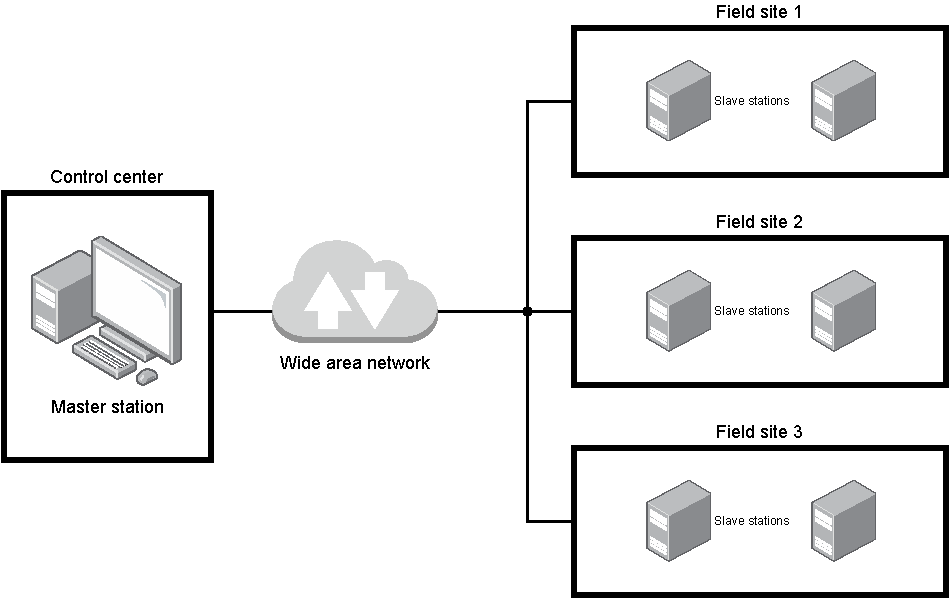
\includegraphics[width=1\textwidth]{obrazky-figures/scada_arch.pdf}
	\caption{Obvykle používáná architektura systémů SCADA. Řídící stanice je umístěna v kontrolním centru a podřízené stanice jsou rozprostřeny do několika fyzicky i logicky oddělených oblastí.}
	\label{fig:scada_arch}
\end{figure}

\subsection{Funkce SCADA systémů}
SCADA systémy nabízejí velké množství monitorovacích a kontrolních funkcí. V následujícím výčtu jsou uvedeny ty nejdůležitější z nich. Převzato z \cite{scada_arch}.
\begin{itemize}
    \item Zobrazení stavu technologických procesů v reálném čase.
    \item Vzdálené řízení technologických procesů pomocí řídící stanice.
    \item Možnost přímých zásahů do technologických procesů operátory.
    \item Automatické řízení technologických procesů za účelem zvýšení efektivity.
    \item Pravidelné generování provozních zpráv.
    \item Grafické zobrazení údajů o technologickém procesu za účelem vypracování efektivních provozních strategií.
\end{itemize}



\subsection{Komunikační standardy SCADA systémů}

Koncem 90. let došlo ke vzniku dvou otevřených komunikačních standardů, známým jako DNP3 a IEC 60870-5, které definují podobu komunikace mezi stanicemi v rámci SCADA systémů. Ta zahrnuje získávání informací a odesílání kontrolních příkazů mezi fyzicky vzdálenými zařízeními. Standardy se vyznačují možností spolehlivého přenosu relativně malých paketů v pevně daném pořadí. V tomto ohledu se liší od více obecně založených protokolů jako je FTP nebo TCP/IP, které nejsou příliš vhodné pro SCADA systémy. Vzhledem ke společnému základu protokolů je funkcionalita na nižších vrstvách podobná. Ve vyšších vrstvách však pracují odlišně \cite{scada_protocols}.

IEC 60870-5 byl vytvořen Mezinárodní elektrotechnickou komisí (dále jen \uv{IEC}, z~anglické zkratky pro \emph{International Electrotechnical Commission}). Standard je primárně využíván v systémech pro správu elektrické přenosové soustavy a to hlavně v evropských zemích \cite{scada_protocols}. V kapitole \ref{iec_104} bude podrobněji rozebrán protokol IEC 60870-5-104, patřící do této rodiny.

DNP3, celým názvem \emph{Distributed Network Protocol 3}, byl navržen společností \emph{Harris} a~určen primárně pro použití v energetickém průmyslu. Na rozdíl od protokolu IEC 60870-5, je však využíván i v jiných odvětvích jako např. plynárenství, zpracování odpadních vod apod. Protokol má velkou podporu v Severní a Jižní Americe, Asii, Jižní Africe a Austrálii \cite{scada_protocols}. Práce se dále tímto standardem zabývat nebude.

\section{Protokol IEC 60870-5-104}

\label{iec_104}

Protokol IEC 60870-5-104 (dále jen \uv{IEC 104}) poskytuje komunikační profil pro zasílání základních telekomunikačních zpráv mezi řídící stanicí a podřízenými stanicemi u SCADA systémů. Vznikl jako nástupce protokolu IEC 60870-5-101 (dále jen \uv{IEC 101}), oproti kterému se liší ve způsobu přenosu informací na nižších vrstvách. Kombinuje aplikační vrstvu protokolu IEC 101 s transportní vrstvou TCP/IP architektury \cite{scada_protocols}. Následující obsah kapitoly se zabývá vlastnostmi aplikační vrstvy a informace v ní obsažené jsou platné pro oba protokoly \cite{iec_104}.

\subsection{Komunikační profil}

Základním předpokladem je rozdělení stanic do hierarchie, kde každá stanice má jasně danou pozici a práva.

\subsubsection*{Typy stanic}

Typ stanice určuje pozici stanice v hierarchii systému.

\begin{itemize}
    \item \textbf{Řídící stanice:} stanice, ze které jsou posílány příkazy podřízeným stanicím. Typicky se jedná o osobní počítač se SCADA systémem, se kterým přímo interaguje operátor systému. Řídící stanice obvykle komunikuje na portu 2404. Někdy je také označována jako \emph{master} nebo \emph{centrální stanice}. 
    \item \textbf{Podřízená stanice:} stanice, která je ovládána řídící stanicí. Může se jednat o senzor, hydraulický lis, turbínu apod. Někdy je také označována jako \emph{slave} nebo \emph{koncová stanice}.
\end{itemize}

\pagebreak

\subsubsection*{Režimy přenosu}

Režim přenosu udává, které stanice mají právo iniciovat komunikaci.

\begin{itemize}
    \item \textbf{Nevyvážený přenos:} řídící stanice reguluje datový provoz podáváním dotazů podřízeným stanicím. Iniciuje všechny přenosy zpráv, zatímco podřízené stanice na tyto zprávy pouze odpovídají.
    \item \textbf{Vyvážený přenos:} jakákoliv stanice má právo iniciovat přenos zprávy. Stanice mohou současně vystupovat jako řídicí a podřízené.
\end{itemize}

\subsubsection*{Směry komunikace}

Směr komunikace udává, odkud kam se přenáší data.

\begin{itemize}
    \item \textbf{Monitorovací směr:} od podřízené stanice k řídící.
    \item \textbf{Kontrolní směr:} od řídící stanice k podřízené.
    \item \textbf{Obrácený směr:} stav, kdy podřízená stanice posílá dotazy a řídící stanice odpovídá daty.
\end{itemize}

\subsection{Struktura aplikačních dat}

Aplikační data protokolu IEC 104 tvoří APDU (Application Protocol Data Unit) jednotka, dělící se dále na APCI (Application Protocol Control Information) a ASDU (Application Service Data Unit), viz ilustrace \ref{apdu_img}.

APCI jednotka začíná 8 bity s fixní hodnotou \texttt{0x68}, za kterými následuje 8 bitů, které udávají délku APDU. Následují čtyři 8 bitové kontrolní pole (\emph{control fields}). 

ASDU jednotka obsahuje 48 bitů pro identifikaci dat a až 127 datových objektů, sloužící k uchování užitečných dat. Některé položky, které slouží k identifikaci jsou dále popsány v~této kapitole  \cite{iec_104}.

\begin{figure}[H]
	\centering
	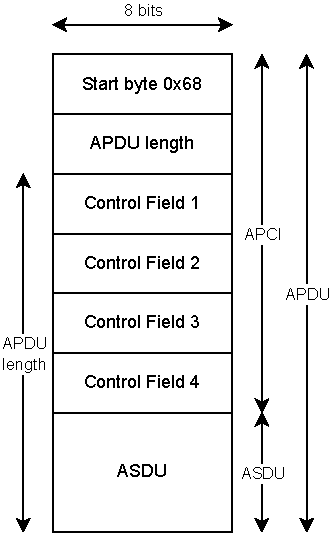
\includegraphics[width=0.32\textwidth]{obrazky-figures/iec104_diagram.pdf}
	\caption{APDU jednotka \cite{iec_104}.}
	\label{apdu_img}
\end{figure}


\subsubsection*{Formát APCI jednotky}
\label{apci_unit}

Protokol IEC 104 definuje celkově 3 formáty, které udávají podobu kontrolních polí. I, S a U formát.
S a I formáty ukládají sekvenční čísla odeslaných zpráv. Pokud je tento čítač neplatný, pak je spojení ukončeno. Možnost zneužití tohoto chování bude popsána v~podkapitole \ref{apci_manipulation}. ASDU je přítomna pouze v případě, že je použit I-formát.

\begin{itemize}
    \item \textbf{I-formát:} z angl. výrazu \emph{Information transfer format}. Slouží k číslovanému přenosu informací mezi řídicí a podřízenou stanicí.
    \item \textbf{S-formát:} z angl. výrazu \emph{numbered supervisory functions}. Používá se k provádění očíslovaných kontrolních funkcí.
    \item \textbf{U-formát:} z angl. výrazu \emph{unnumbered control functions}. Slouží k provádění nečíslovaných řídicích funkcí.
\end{itemize}


\subsubsection*{Položky ASDU}
\label{polozky_asdu}

\emph{Poznámka: V následujícím výčtu jsou uvedeny pouze položky relevantní pro tuhle práci.}

\begin{itemize}
    \item \textbf{Typ:} Udává typ přenášených dat.
    \item \textbf{COT:} Důvod přenosu, z angl. zkratky pro \emph{cause of transmission}. Používá se při interpretaci dat cílovou stanicí. Každý typ ASDU má definovanou podmnožinu platných COT kódů, které jsou pro něj smysluplné.
    \item \textbf{COA:} Společná ASDU adresa, z angl. zkratky pro \emph{common ASDU address}. Je asociovaná se všemi datovými objekty v ASDU bloku. Většinou je používána pro identifikaci celé stanice. Alternativní možností je identifikace sektoru stanice, při které lze stanici rozdělit na několik logických částí.
    \item \textbf{IOA:} Adresa informačního objektu, z angl. zkratky pro \emph{Information object address}. Slouží k identifikaci konkrétních dat konkrétní stanice.
\end{itemize}


\section{Útoky na SCADA systémy}
\label{scada_attacks}

Přestože je protokol IEC 104 široce využíván, zabezpečení nebylo při vzniku prioritou. Protokol postrádá důležité bezpečnostní prvky jako je šifrování, ochrana integrity nebo autentizace. V této podkapitole budou představeny některé kybernetické útoky, vůči kterým nemá protokol vestavěnou ochranu. Následující výčet útoků čerpá z \cite{scada_attack}.



\subsection*{Neautentizovaný přístup}
\label{unauthorized_access}


Protokol nedisponuje mechanismem ověření identity. Útočník se může připojit ke koncové stanici a bez nutnosti autentizace začít odesílat kontrolní příkazy. Útočník může například odeslat dotazovací příkaz a zjistit stanicí používané hodnoty IOA (viz \ref{polozky_asdu}) . Typický průběh útoku vypadá následovně:


\begin{enumerate}
    \item Zjištění IP adresy a portu koncové stanice.
    \item Vydávání se za řídící stanici a odeslání požadavku na připojení koncové stanici.
    \item Kvůli chybějící autentizaci, dojde ze strany koncové stanice k přijetí požadavku.
    \item Odeslání libovolných kontrolních příkazů koncové stanici.
\end{enumerate}


\subsection*{Manipulace sekvenčních čísel APCI}
\label{apci_manipulation}

Pokud stanice obdrží paket s neočekávaným sekvenčním číslem v jednotce APCI, dojde k ukončení spojení. Útočník může zneužít této vlastnosti a následujícími kroky zapříčinit výpadek systému (tzv. \emph{Denial of Service}): 

\begin{enumerate}
    \item Vložení se do komunikace mezi stanicemi. Z útočníka se stane tzv. \emph{Man in the middle}.
    \item Odchycení příchozích paketů.
    \item Modifikace paketů. Konkrétně změna pořadového čísla APCI.
    \item Výpočet nového \emph{TCP checksum}.
    \item Navrácení paketů do původní komunikace.
\end{enumerate}


\subsection*{Manipulace TCP toku}

Komunikace mezi řídící a koncovou stanicí probíhá v jednom TCP proudu, který je aktivně udržován otevřený.
Útočník, který vystupuje jako \emph{Man in the middle}, může využít zranitelnosti TCP a způsobit ukončení komunikace, vedoucí k nesprávné funkci nebo dokonce výpadku systému. Tento typ útoku se liší od \ref{apci_manipulation} pouze ve třetím bodě. V tomto případě mohou být k modifikaci paketů použity následující metody:

\begin{itemize}
    \item Sekvenční číslo TCP toku se změní na neočekávanou hodnotu.
    \item Synchronizační příznak se nastaví na hodnotu \texttt{FIN}\footnote{Příznak \texttt{FIN} se používá u TCP komunikace k označení jejího konce.}.
\end{itemize}


\subsection*{Záplava pakety s příznakem SYN}

Jedná se o běžný kybernetický útok, v anglickém jazyce je znám pod pojmem \emph{SYN Flood}. Během útoku se útočník snaží zahltit cílový systém velkým množstvím paketů se synchronizačním příznakem nastaveným na hodnotu \texttt{SYN}\footnote{Příznak \texttt{SYN} se používá u TCP komunikace k vyžádání nového spojení.}. Cílové stanice jsou zahlceny množstvím nových falešných žádostí o spojení a nestíhají odbavovat legitimní požadavky. Dochází k~znatelnému zpomalení systému \cite{radoglou}.



\subsection*{Vkládání podvržených paketů}

Jedná se o pokročilou formu útoku, která umožňuje útočníkovi v pozici \emph{Man in the middle} vkládat do komunikace pakety s libovolnými hodnotami ASDU. Útočník tak může převzít ovládání nad celou energetickou sítí. K úspěšnému provedení útoku musí útočník správně upravit sekvenční čísla (APCI i TCP) všech paketů. V~případě, že by tak neučinil, došlo by k ukončení spojení. Detekce takového útoku může být velmi obtížná, jelikož nedochází k přerušení spojení a navíc může útočník podvrhnout data, která se budou zobrazovat operátorovi. Typický průběh útoku:

\begin{enumerate}
    \item Vložení se do komunikace mezi stanicemi. Z útočníka se stane tzv. Man in the middle.
    \item Odchycení příchozích paketů a učení se APCI a TCP sekvencí.
    \item Vložení podvrženého paketu s libovolnou hodnotou ASDU a vypozorovanými sekvenčními čísly do komunikace.
    \item Sledování a udržování vnitřního stavu sekvenčních čísel.
    \item Zachycení všech zbylých paketů a opravení sekvenčních čísel tak, aby spojení nebylo přerušeno.
\end{enumerate}

\chapter{Statistický popis dat}
\label{chapter_stats}

Statistickým popisem dat se zabývá tzv. \emph{deskriptivní statistika}. Jedná se o disciplínu, která kvantitativně popisuje hlavní vlastnosti souboru dat a snaží se numerickým nebo grafickým popisem vystihnout podstatné informace o daných datech. Umožňuje uživateli nalézt rozložení hodnot atributů a tím pádem lépe pochopit zkoumaná data. Předmětem zkoumání deskriptivní statistiky je statistický soubor dat, který může reprezentovat buď celou populaci, nebo pouze její část (tzv. \emph{výběrový soubor}).

Numerický popis dat se člení na míry polohy (viz \ref{avg_stats}) a míry variability (viz \ref{var_stats}). Mezi míry polohy patří např. modus, medián nebo střední hodnota. Mezi míry variability patří např. rozptyl, směrodatná odchylka, minimum, maximum apod. Grafický popis dat nabízí velké množství metod zobrazení, z nichž nejčastěji používané jsou např. spojnicové grafy, histogramy, koláčové grafy apod. Vybrané metody budou popsány v podkapitole \ref{charts}.  


\section{Míry polohy}
\label{avg_stats}

Míry polohy vyjadřují \uv{kde} se data nacházejí. Charakterizují \uv{střed} datového souboru, kolem kterého se hodnoty pohybují. Mají důležitou výpovědní hodnotu o tom, jak data vypadají a jak se chovají. Mohou nabývat i takových hodnot, které se v datovém souboru přímo nenacházejí, například průměrná hodnota v souboru přirozených čísel může být racionálním číslem, které není přirozené. Pro charakteristiky polohy výběrového souboru platí, že pouze odhadují skutečné hodnoty celé populace \cite{average}.


\subsection*{Střední hodnota}

Střední hodnota datového souboru je nejzákladnější charakteristikou polohy. Označuje se řeckým písmenem $\mu$ a je totožná s aritmetickým průměrem všech prvků souboru. Význam střední hodnoty je největší u datových souborů se symetrickým rozdělením dat a s nízkým výskytem odlehlých hodnot. V takovém případě by měla rozdělovat soubor na dva přibližně stejně velké celky. Tahle vlastnost je negativně ovlivňována výskytem odlehlých hodnot, které mají schopnost výrazně vychýlit střední hodnotu. Střední hodnota se počítá jako součet všech hodnot vydělených jejich počtem \cite{skiena}:


\begin{equation}
\mu = \frac{1}{N} \sum_{i=1}^{N} x_{i}
\end{equation}

\noindent kde:



\begin{description}
    \item[N] je celkový počet prvků v datovém souboru.
    \item[x_i] je \emph{i}-tý prvek datového souboru.
\end{description}


\noindent Důležitou vlastností průměru (a tím pádem i střední hodnoty) je \uv{nevychýlenost}, která zajišťuje, že průměr všech možných výběrových průměrů, počítaný přes všechny výběrové soubory dané velikosti, je roven průměru celé populace. Díky této vlastnosti je zajištěno, že průměr výběrového souboru dobře aproximuje průměr celé populace a tudíž je jeho výpovědní hodnota relevantní i přes neúplnost dat \cite{zahora}.

\subsection*{Medián}

Medián je přesným středem datové sady. Rozděluje sadu na dvě stejně velké části, kde počet prvků s větší hodnotou než medián je stejný jako počet prvků s hodnotou menší. V případě lichého počtu prvků v datové sadě je mediánem \uv{prostřední} prvek seřazené datové sady \ref{med_odd}. Pro sady se sudým počtem prvků je mediánem průměr dvou \uv{prostředních} prvků seřazené datové sady \ref{med_even}.
Čím více je distribuce dat symetrická, tím leží medián blíže střední hodnotě a přidaná výpovědní hodnota není příliš vysoká. U datových sad s asymetrickým rozložením může však vzdálenost a vzájemná poloha mediánu a střední hodnoty napovědět hodně o tom, jak vypadá distribuce a jak moc je asymetrická. Výrazně se lišící hodnoty navíc naznačují, že se v datové sadě nachází mnoho odlehlých hodnot, které ovlivňují střední hodnotu \cite{skiena}.


\begin{align}
    & & Med & =  x_{\frac{N+1}{2}} & \text{pro lichá } N & &  \label{med_odd}\\
    & & Med & =  \frac{x_{\frac{N}{2}}+x_{\frac{N}{2}+1}}{2} & \text{pro sudá } N & & \label{med_even}
\end{align}

\noindent kde:



\begin{description}
    \item[N] je celkový počet prvků v datovém souboru.
    \item[x_n] je \emph{n}-tý prvek seřazeného datového souboru.
\end{description}


\subsection*{Modus}

Modus je nejčastější hodnota, která se vyskytuje v datové sadě. Při jeho výpočtu se většinou datová sada rozdělí do intervalů, ve kterých se nalezne ten nejvíce zastoupený a jako modus se použije jeho střed krajních hodnot. Často je využíván k detekci chyb nebo anomálií (v datové sadě může být například nejčastější hodnotou výchozí nebo chybová hodnota). Datové sady, pro které modus nabývá více hodnot, označujeme jako \emph{multimodální}. Multimodalita může naznačovat, že v datový soubor vznikl smícháním dvou nebo více unimodálních populací \cite{zahora}.

\subsection*{Q-Kvantily}

$q$-kvantily rozdělují seřazený soubor dat na $q$ přibližně stejně velkých částí. $k$-tý $q$-kvantil je hodnota $Q_k$ náhodné veličiny $X$, pro kterou za předpokladu že:

\begin{equation*}
    0 < k < q \wedge k, q \in \mathbb{N}
\end{equation*}

platí:

\begin{equation}
    P(X \leq  Q_k)\geq \frac{k}{q} \wedge P(X \geq Q_k) \geq 1 - \frac{k}{q}
\end{equation}

\medskip

Pro následující hodnoty $q$ se $q$-kvantily označují jako:
\begin{itemize}
    \item $q=2$: medián
    \item $q=3$: tercil
    \item $q=4$: kvartil
    \item $q=5$: kvintil
    \item $q=10$: decil
    \item $q=100$: percentil
\end{itemize}


\section{Míry variability}
\label{var_stats}

Míry variability zkoumají, jak jsou prvky v datovém souboru vzájemně blízké či vzdálené. Hodnotí rozptýlenost hodnot statistického souboru kolem nějaké střední hodnoty. Pro charakteristiky variability výběrového souboru opět platí, že pouze odhadují skutečné hodnoty celé populace \cite{variance}.


\subsection*{Směrodatná odchylka a rozptyl}
Nejběžnějším měřítkem variability je rozptyl, který se označuje symbolem $\sigma^2$. Udává, jak moc jsou data soustředěna kolem střední hodnoty. Nízký rozptyl naznačuje, že datové body mají tendenci být těsně seskupeny kolem středu. Vysoký rozptyl naopak znamená, že mají tendenci se od středu vzdalovat. Kromě rozptylu se často používá i směrodatná odchylka, která je druhou odmocninou rozptylu a označuje se symbolem $\sigma$. Pro výpočet rozptylu se používá součet čtverců odchylek jednotlivých prvků od střední hodnoty \cite{frost}:

\begin{equation}
    \sigma^2 = \frac{1}{N-1} \sum_{i=1}^{N} (x_i - \mu)^2
\end{equation}

\noindent Pro výpočet směrodatné odchylky poté použijeme druhou odmocninu rozptylu:

\begin{equation}
    \sigma = \sqrt{\sigma^2}
\end{equation}

\medskip

\noindent Pro datový soubor s distribucí, která se alespoň přibližně řídí normálním rozdělením, lze pomocí směrodatné odchylky odhadnout podíly hodnot, které spadají do určitých intervalů. Přibližné rozložení dat je ukázáno na obrázku \ref{fig:normal_distribution} a platí pro něj platí následující vlastnosti \cite{frost}:

\begin{itemize}
    \item V intervalu $\langle{\mu-\sigma,\mu+\sigma}\rangle$ leží přibližně 68~\% hodnot.
    \item V intervalu $\langle{\mu-2\sigma,\mu+2\sigma}\rangle$ leží přibližně 95~\% hodnot.
    \item V intervalu $\langle{\mu-3\sigma,\mu+3\sigma}\rangle$ leží přibližně 99,7~\% hodnot.
\end{itemize}

\begin{figure}[H]
	\centering
	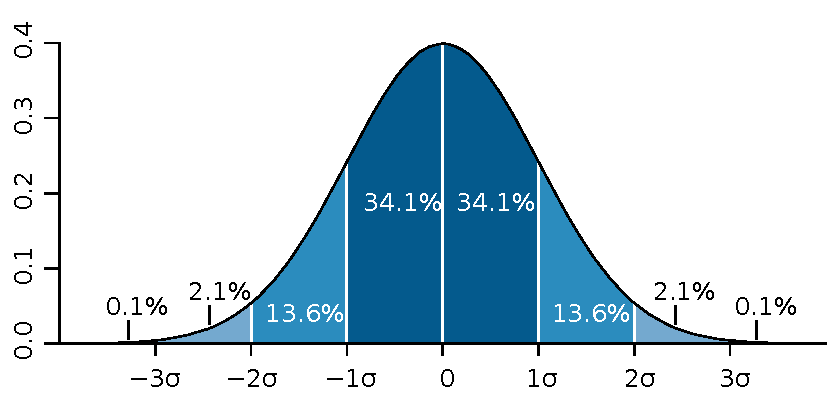
\includegraphics[width=0.9\textwidth]{obrazky-figures/normal_distribution.pdf}
	\caption{Ukázka rozložení dat u normálního rozdělení \cite{normal_distribution}.}
	\label{fig:normal_distribution}
\end{figure}


\subsection*{Variační šíře}

Udává rozdíl mezi největší a nejmenší hodnotou v datovém souboru. Je přímo ovlivněna extrémními hodnotami. Nejedná se o interval, ale o číslo udávající šíři intervalu. Výpočet vypadá následovně \cite{variance}:

\begin{equation}
    R = x_{max} - x_{min}
\end{equation}

\noindent kde:

\begin{description}
    \item[x_n] je \emph{n}-tý prvek seřazeného datového souboru.
\end{description}

\subsection*{Mezikvartilové rozpětí}



Mezikvartilové rozpětí (angl. \emph{Interquartile range}, zkratka IQR) udává šířku oblasti, ve které leží středních 50 \% hodnot. Nabízí uživateli robustní alternativu ke klasickému rozptylu, která není ovlivňována odlehlými hodnotami.  Počítá se jako rozdíl mezi třetím a prvním kvartilem (tedy mezi 75. a 25. percentilem) \cite{frost}:

\begin{equation}
    IQR = q_3 - q_1 = p_{75} - p_{25}
\end{equation}

\noindent kde:

\begin{description}
    \item[q_n] je \emph{n}-tý kvantil.
    \item[p_n] je \emph{n}-tý percentil.
\end{description}



\noindent Pomocí mezikvartilového rozpětí lze provést detekci odlehlých hodnot. Jelikož jimi není ovlivňováno, snižuje se oproti jiným metodám pravděpodobnost selhání. Metoda navíc nepředpokládá normální rozdělení dat. K detekci se používají tzv. brány, které jsou definovány následujícím způsobem \cite{frost2}:

\begin{gather}
    lower\_gate = q_1-1.5 \cdot IQR \\
    upper\_gate = q_3+1.5 \cdot IQR
\end{gather}

\noindent Pro odlehlé hodnoty $x$ potom platí:

\begin{equation}
    x < lower\_gate \lor x > upper\_gate
\end{equation}



\section{Vizualizační metody popisu dat}
\label{charts}



Vizualizační metody jsou důležitou součástí popisné statistiky, která efektivně ukazuje kvantitativní vlastnosti datových souborů jako je rozložení hodnot jejich atributů. Může se jednat o přehledové tabulky, různé druhy grafů, histogramy apod. Mezi nejdůležitější aspekty grafického popisu dat patří následující \cite{skiena}:

\begin{itemize}
    \item \textbf{Explorační funkce:} usnadňuje uživateli orientaci v datech. Pro uživatele je snazší pochopit chování a distribuci dat.
    \item \textbf{Detekce chyb:} usnadňuje uživateli nalezení chyb a anomálii v datovém souboru. Může se jednat o špatně naměřené hodnoty, nesprávně načtená data atd.
    \item \textbf{Komunikační funkce:} umožňuje snadno data prezentovat ostatním uživatelům, kteří nemají hluboký vhled do aplikační domény a neznají kontext vzniku datového souboru.
\end{itemize}

\subsection*{Histogram}

Histogram je sloupcový graf, který znázorňuje absolutní nebo relativní četnosti hodnot nějakého atributu datové sady \cite{zahora}. Příklad histogramu je uveden na obrázku \ref{hist_plots}. Na vodorovnou osu jsou vyneseny hodnoty atributu a na svislou osu (relativní) četnosti. Někdy je histogram doplněn o křivku znázorňující odhad funkce hustoty pravděpodobnosti (viz obrázek \ref{sub:distplot}). Další častá úprava histogramu spočívá v tom, že namísto vynesení samostatného sloupce pro každou hodnotu atributu, jsou hodnoty atributů rozděleny do intervalů (tříd) a~sloupce jsou vyneseny až pro tyhle intervaly. V takovém případě je důležité zvolit správnou velikost intervalu. Příliš malé intervaly mohou způsobit, že hodnot které do nich spadají, bude příliš málo, nebo že šum bude rušit čitelnost a přehlednost histogramu. Naopak příliš velké intervaly mohou způsobit ztrátu informace o rozdělení, podle kterého se data řídí \cite{skiena}. 

\begin{figure}[h]%
    \centering
    \begin{subfigure}{0.5\textwidth}
        \centering
        \resizebox{1\textwidth}{!}
        {
            %% Creator: Matplotlib, PGF backend
%%
%% To include the figure in your LaTeX document, write
%%   \input{<filename>.pgf}
%%
%% Make sure the required packages are loaded in your preamble
%%   \usepackage{pgf}
%%
%% Also ensure that all the required font packages are loaded; for instance,
%% the lmodern package is sometimes necessary when using math font.
%%   \usepackage{lmodern}
%%
%% Figures using additional raster images can only be included by \input if
%% they are in the same directory as the main LaTeX file. For loading figures
%% from other directories you can use the `import` package
%%   \usepackage{import}
%%
%% and then include the figures with
%%   \import{<path to file>}{<filename>.pgf}
%%
%% Matplotlib used the following preamble
%%   \usepackage{fontspec}
%%   \setmainfont{DejaVuSerif.ttf}[Path=\detokenize{/home/ankimme/fit/ibt/env/lib/python3.10/site-packages/matplotlib/mpl-data/fonts/ttf/}]
%%   \setsansfont{DejaVuSans.ttf}[Path=\detokenize{/home/ankimme/fit/ibt/env/lib/python3.10/site-packages/matplotlib/mpl-data/fonts/ttf/}]
%%   \setmonofont{DejaVuSansMono.ttf}[Path=\detokenize{/home/ankimme/fit/ibt/env/lib/python3.10/site-packages/matplotlib/mpl-data/fonts/ttf/}]
%%
\begingroup%
\makeatletter%
\begin{pgfpicture}%
\pgfpathrectangle{\pgfpointorigin}{\pgfqpoint{5.000000in}{4.000000in}}%
\pgfusepath{use as bounding box, clip}%
\begin{pgfscope}%
\pgfsetbuttcap%
\pgfsetmiterjoin%
\pgfsetlinewidth{0.000000pt}%
\definecolor{currentstroke}{rgb}{1.000000,1.000000,1.000000}%
\pgfsetstrokecolor{currentstroke}%
\pgfsetstrokeopacity{0.000000}%
\pgfsetdash{}{0pt}%
\pgfpathmoveto{\pgfqpoint{0.000000in}{0.000000in}}%
\pgfpathlineto{\pgfqpoint{5.000000in}{0.000000in}}%
\pgfpathlineto{\pgfqpoint{5.000000in}{4.000000in}}%
\pgfpathlineto{\pgfqpoint{0.000000in}{4.000000in}}%
\pgfpathlineto{\pgfqpoint{0.000000in}{0.000000in}}%
\pgfpathclose%
\pgfusepath{}%
\end{pgfscope}%
\begin{pgfscope}%
\pgfsetbuttcap%
\pgfsetmiterjoin%
\definecolor{currentfill}{rgb}{1.000000,1.000000,1.000000}%
\pgfsetfillcolor{currentfill}%
\pgfsetlinewidth{0.000000pt}%
\definecolor{currentstroke}{rgb}{0.000000,0.000000,0.000000}%
\pgfsetstrokecolor{currentstroke}%
\pgfsetstrokeopacity{0.000000}%
\pgfsetdash{}{0pt}%
\pgfpathmoveto{\pgfqpoint{0.630049in}{0.570804in}}%
\pgfpathlineto{\pgfqpoint{4.958330in}{0.570804in}}%
\pgfpathlineto{\pgfqpoint{4.958330in}{3.958330in}}%
\pgfpathlineto{\pgfqpoint{0.630049in}{3.958330in}}%
\pgfpathlineto{\pgfqpoint{0.630049in}{0.570804in}}%
\pgfpathclose%
\pgfusepath{fill}%
\end{pgfscope}%
\begin{pgfscope}%
\pgfpathrectangle{\pgfqpoint{0.630049in}{0.570804in}}{\pgfqpoint{4.328281in}{3.387526in}}%
\pgfusepath{clip}%
\pgfsetbuttcap%
\pgfsetmiterjoin%
\definecolor{currentfill}{rgb}{0.121569,0.466667,0.705882}%
\pgfsetfillcolor{currentfill}%
\pgfsetfillopacity{0.750000}%
\pgfsetlinewidth{1.003750pt}%
\definecolor{currentstroke}{rgb}{0.000000,0.000000,0.000000}%
\pgfsetstrokecolor{currentstroke}%
\pgfsetdash{}{0pt}%
\pgfpathmoveto{\pgfqpoint{0.826789in}{0.570804in}}%
\pgfpathlineto{\pgfqpoint{1.129466in}{0.570804in}}%
\pgfpathlineto{\pgfqpoint{1.129466in}{0.885557in}}%
\pgfpathlineto{\pgfqpoint{0.826789in}{0.885557in}}%
\pgfpathlineto{\pgfqpoint{0.826789in}{0.570804in}}%
\pgfpathclose%
\pgfusepath{stroke,fill}%
\end{pgfscope}%
\begin{pgfscope}%
\pgfpathrectangle{\pgfqpoint{0.630049in}{0.570804in}}{\pgfqpoint{4.328281in}{3.387526in}}%
\pgfusepath{clip}%
\pgfsetbuttcap%
\pgfsetmiterjoin%
\definecolor{currentfill}{rgb}{0.121569,0.466667,0.705882}%
\pgfsetfillcolor{currentfill}%
\pgfsetfillopacity{0.750000}%
\pgfsetlinewidth{1.003750pt}%
\definecolor{currentstroke}{rgb}{0.000000,0.000000,0.000000}%
\pgfsetstrokecolor{currentstroke}%
\pgfsetdash{}{0pt}%
\pgfpathmoveto{\pgfqpoint{1.129466in}{0.570804in}}%
\pgfpathlineto{\pgfqpoint{1.432143in}{0.570804in}}%
\pgfpathlineto{\pgfqpoint{1.432143in}{0.649492in}}%
\pgfpathlineto{\pgfqpoint{1.129466in}{0.649492in}}%
\pgfpathlineto{\pgfqpoint{1.129466in}{0.570804in}}%
\pgfpathclose%
\pgfusepath{stroke,fill}%
\end{pgfscope}%
\begin{pgfscope}%
\pgfpathrectangle{\pgfqpoint{0.630049in}{0.570804in}}{\pgfqpoint{4.328281in}{3.387526in}}%
\pgfusepath{clip}%
\pgfsetbuttcap%
\pgfsetmiterjoin%
\definecolor{currentfill}{rgb}{0.121569,0.466667,0.705882}%
\pgfsetfillcolor{currentfill}%
\pgfsetfillopacity{0.750000}%
\pgfsetlinewidth{1.003750pt}%
\definecolor{currentstroke}{rgb}{0.000000,0.000000,0.000000}%
\pgfsetstrokecolor{currentstroke}%
\pgfsetdash{}{0pt}%
\pgfpathmoveto{\pgfqpoint{1.432143in}{0.570804in}}%
\pgfpathlineto{\pgfqpoint{1.734820in}{0.570804in}}%
\pgfpathlineto{\pgfqpoint{1.734820in}{1.515062in}}%
\pgfpathlineto{\pgfqpoint{1.432143in}{1.515062in}}%
\pgfpathlineto{\pgfqpoint{1.432143in}{0.570804in}}%
\pgfpathclose%
\pgfusepath{stroke,fill}%
\end{pgfscope}%
\begin{pgfscope}%
\pgfpathrectangle{\pgfqpoint{0.630049in}{0.570804in}}{\pgfqpoint{4.328281in}{3.387526in}}%
\pgfusepath{clip}%
\pgfsetbuttcap%
\pgfsetmiterjoin%
\definecolor{currentfill}{rgb}{0.121569,0.466667,0.705882}%
\pgfsetfillcolor{currentfill}%
\pgfsetfillopacity{0.750000}%
\pgfsetlinewidth{1.003750pt}%
\definecolor{currentstroke}{rgb}{0.000000,0.000000,0.000000}%
\pgfsetstrokecolor{currentstroke}%
\pgfsetdash{}{0pt}%
\pgfpathmoveto{\pgfqpoint{1.734820in}{0.570804in}}%
\pgfpathlineto{\pgfqpoint{2.037497in}{0.570804in}}%
\pgfpathlineto{\pgfqpoint{2.037497in}{1.751127in}}%
\pgfpathlineto{\pgfqpoint{1.734820in}{1.751127in}}%
\pgfpathlineto{\pgfqpoint{1.734820in}{0.570804in}}%
\pgfpathclose%
\pgfusepath{stroke,fill}%
\end{pgfscope}%
\begin{pgfscope}%
\pgfpathrectangle{\pgfqpoint{0.630049in}{0.570804in}}{\pgfqpoint{4.328281in}{3.387526in}}%
\pgfusepath{clip}%
\pgfsetbuttcap%
\pgfsetmiterjoin%
\definecolor{currentfill}{rgb}{0.121569,0.466667,0.705882}%
\pgfsetfillcolor{currentfill}%
\pgfsetfillopacity{0.750000}%
\pgfsetlinewidth{1.003750pt}%
\definecolor{currentstroke}{rgb}{0.000000,0.000000,0.000000}%
\pgfsetstrokecolor{currentstroke}%
\pgfsetdash{}{0pt}%
\pgfpathmoveto{\pgfqpoint{2.037497in}{0.570804in}}%
\pgfpathlineto{\pgfqpoint{2.340174in}{0.570804in}}%
\pgfpathlineto{\pgfqpoint{2.340174in}{2.931449in}}%
\pgfpathlineto{\pgfqpoint{2.037497in}{2.931449in}}%
\pgfpathlineto{\pgfqpoint{2.037497in}{0.570804in}}%
\pgfpathclose%
\pgfusepath{stroke,fill}%
\end{pgfscope}%
\begin{pgfscope}%
\pgfpathrectangle{\pgfqpoint{0.630049in}{0.570804in}}{\pgfqpoint{4.328281in}{3.387526in}}%
\pgfusepath{clip}%
\pgfsetbuttcap%
\pgfsetmiterjoin%
\definecolor{currentfill}{rgb}{0.121569,0.466667,0.705882}%
\pgfsetfillcolor{currentfill}%
\pgfsetfillopacity{0.750000}%
\pgfsetlinewidth{1.003750pt}%
\definecolor{currentstroke}{rgb}{0.000000,0.000000,0.000000}%
\pgfsetstrokecolor{currentstroke}%
\pgfsetdash{}{0pt}%
\pgfpathmoveto{\pgfqpoint{2.340174in}{0.570804in}}%
\pgfpathlineto{\pgfqpoint{2.642851in}{0.570804in}}%
\pgfpathlineto{\pgfqpoint{2.642851in}{3.639643in}}%
\pgfpathlineto{\pgfqpoint{2.340174in}{3.639643in}}%
\pgfpathlineto{\pgfqpoint{2.340174in}{0.570804in}}%
\pgfpathclose%
\pgfusepath{stroke,fill}%
\end{pgfscope}%
\begin{pgfscope}%
\pgfpathrectangle{\pgfqpoint{0.630049in}{0.570804in}}{\pgfqpoint{4.328281in}{3.387526in}}%
\pgfusepath{clip}%
\pgfsetbuttcap%
\pgfsetmiterjoin%
\definecolor{currentfill}{rgb}{0.121569,0.466667,0.705882}%
\pgfsetfillcolor{currentfill}%
\pgfsetfillopacity{0.750000}%
\pgfsetlinewidth{1.003750pt}%
\definecolor{currentstroke}{rgb}{0.000000,0.000000,0.000000}%
\pgfsetstrokecolor{currentstroke}%
\pgfsetdash{}{0pt}%
\pgfpathmoveto{\pgfqpoint{2.642851in}{0.570804in}}%
\pgfpathlineto{\pgfqpoint{2.945528in}{0.570804in}}%
\pgfpathlineto{\pgfqpoint{2.945528in}{3.167514in}}%
\pgfpathlineto{\pgfqpoint{2.642851in}{3.167514in}}%
\pgfpathlineto{\pgfqpoint{2.642851in}{0.570804in}}%
\pgfpathclose%
\pgfusepath{stroke,fill}%
\end{pgfscope}%
\begin{pgfscope}%
\pgfpathrectangle{\pgfqpoint{0.630049in}{0.570804in}}{\pgfqpoint{4.328281in}{3.387526in}}%
\pgfusepath{clip}%
\pgfsetbuttcap%
\pgfsetmiterjoin%
\definecolor{currentfill}{rgb}{0.121569,0.466667,0.705882}%
\pgfsetfillcolor{currentfill}%
\pgfsetfillopacity{0.750000}%
\pgfsetlinewidth{1.003750pt}%
\definecolor{currentstroke}{rgb}{0.000000,0.000000,0.000000}%
\pgfsetstrokecolor{currentstroke}%
\pgfsetdash{}{0pt}%
\pgfpathmoveto{\pgfqpoint{2.945528in}{0.570804in}}%
\pgfpathlineto{\pgfqpoint{3.248205in}{0.570804in}}%
\pgfpathlineto{\pgfqpoint{3.248205in}{3.797019in}}%
\pgfpathlineto{\pgfqpoint{2.945528in}{3.797019in}}%
\pgfpathlineto{\pgfqpoint{2.945528in}{0.570804in}}%
\pgfpathclose%
\pgfusepath{stroke,fill}%
\end{pgfscope}%
\begin{pgfscope}%
\pgfpathrectangle{\pgfqpoint{0.630049in}{0.570804in}}{\pgfqpoint{4.328281in}{3.387526in}}%
\pgfusepath{clip}%
\pgfsetbuttcap%
\pgfsetmiterjoin%
\definecolor{currentfill}{rgb}{0.121569,0.466667,0.705882}%
\pgfsetfillcolor{currentfill}%
\pgfsetfillopacity{0.750000}%
\pgfsetlinewidth{1.003750pt}%
\definecolor{currentstroke}{rgb}{0.000000,0.000000,0.000000}%
\pgfsetstrokecolor{currentstroke}%
\pgfsetdash{}{0pt}%
\pgfpathmoveto{\pgfqpoint{3.248205in}{0.570804in}}%
\pgfpathlineto{\pgfqpoint{3.550882in}{0.570804in}}%
\pgfpathlineto{\pgfqpoint{3.550882in}{3.088826in}}%
\pgfpathlineto{\pgfqpoint{3.248205in}{3.088826in}}%
\pgfpathlineto{\pgfqpoint{3.248205in}{0.570804in}}%
\pgfpathclose%
\pgfusepath{stroke,fill}%
\end{pgfscope}%
\begin{pgfscope}%
\pgfpathrectangle{\pgfqpoint{0.630049in}{0.570804in}}{\pgfqpoint{4.328281in}{3.387526in}}%
\pgfusepath{clip}%
\pgfsetbuttcap%
\pgfsetmiterjoin%
\definecolor{currentfill}{rgb}{0.121569,0.466667,0.705882}%
\pgfsetfillcolor{currentfill}%
\pgfsetfillopacity{0.750000}%
\pgfsetlinewidth{1.003750pt}%
\definecolor{currentstroke}{rgb}{0.000000,0.000000,0.000000}%
\pgfsetstrokecolor{currentstroke}%
\pgfsetdash{}{0pt}%
\pgfpathmoveto{\pgfqpoint{3.550882in}{0.570804in}}%
\pgfpathlineto{\pgfqpoint{3.853559in}{0.570804in}}%
\pgfpathlineto{\pgfqpoint{3.853559in}{2.616697in}}%
\pgfpathlineto{\pgfqpoint{3.550882in}{2.616697in}}%
\pgfpathlineto{\pgfqpoint{3.550882in}{0.570804in}}%
\pgfpathclose%
\pgfusepath{stroke,fill}%
\end{pgfscope}%
\begin{pgfscope}%
\pgfpathrectangle{\pgfqpoint{0.630049in}{0.570804in}}{\pgfqpoint{4.328281in}{3.387526in}}%
\pgfusepath{clip}%
\pgfsetbuttcap%
\pgfsetmiterjoin%
\definecolor{currentfill}{rgb}{0.121569,0.466667,0.705882}%
\pgfsetfillcolor{currentfill}%
\pgfsetfillopacity{0.750000}%
\pgfsetlinewidth{1.003750pt}%
\definecolor{currentstroke}{rgb}{0.000000,0.000000,0.000000}%
\pgfsetstrokecolor{currentstroke}%
\pgfsetdash{}{0pt}%
\pgfpathmoveto{\pgfqpoint{3.853559in}{0.570804in}}%
\pgfpathlineto{\pgfqpoint{4.156236in}{0.570804in}}%
\pgfpathlineto{\pgfqpoint{4.156236in}{1.121621in}}%
\pgfpathlineto{\pgfqpoint{3.853559in}{1.121621in}}%
\pgfpathlineto{\pgfqpoint{3.853559in}{0.570804in}}%
\pgfpathclose%
\pgfusepath{stroke,fill}%
\end{pgfscope}%
\begin{pgfscope}%
\pgfpathrectangle{\pgfqpoint{0.630049in}{0.570804in}}{\pgfqpoint{4.328281in}{3.387526in}}%
\pgfusepath{clip}%
\pgfsetbuttcap%
\pgfsetmiterjoin%
\definecolor{currentfill}{rgb}{0.121569,0.466667,0.705882}%
\pgfsetfillcolor{currentfill}%
\pgfsetfillopacity{0.750000}%
\pgfsetlinewidth{1.003750pt}%
\definecolor{currentstroke}{rgb}{0.000000,0.000000,0.000000}%
\pgfsetstrokecolor{currentstroke}%
\pgfsetdash{}{0pt}%
\pgfpathmoveto{\pgfqpoint{4.156236in}{0.570804in}}%
\pgfpathlineto{\pgfqpoint{4.458913in}{0.570804in}}%
\pgfpathlineto{\pgfqpoint{4.458913in}{1.121621in}}%
\pgfpathlineto{\pgfqpoint{4.156236in}{1.121621in}}%
\pgfpathlineto{\pgfqpoint{4.156236in}{0.570804in}}%
\pgfpathclose%
\pgfusepath{stroke,fill}%
\end{pgfscope}%
\begin{pgfscope}%
\pgfpathrectangle{\pgfqpoint{0.630049in}{0.570804in}}{\pgfqpoint{4.328281in}{3.387526in}}%
\pgfusepath{clip}%
\pgfsetbuttcap%
\pgfsetmiterjoin%
\definecolor{currentfill}{rgb}{0.121569,0.466667,0.705882}%
\pgfsetfillcolor{currentfill}%
\pgfsetfillopacity{0.750000}%
\pgfsetlinewidth{1.003750pt}%
\definecolor{currentstroke}{rgb}{0.000000,0.000000,0.000000}%
\pgfsetstrokecolor{currentstroke}%
\pgfsetdash{}{0pt}%
\pgfpathmoveto{\pgfqpoint{4.458913in}{0.570804in}}%
\pgfpathlineto{\pgfqpoint{4.761590in}{0.570804in}}%
\pgfpathlineto{\pgfqpoint{4.761590in}{0.806868in}}%
\pgfpathlineto{\pgfqpoint{4.458913in}{0.806868in}}%
\pgfpathlineto{\pgfqpoint{4.458913in}{0.570804in}}%
\pgfpathclose%
\pgfusepath{stroke,fill}%
\end{pgfscope}%
\begin{pgfscope}%
\pgfsetbuttcap%
\pgfsetroundjoin%
\definecolor{currentfill}{rgb}{0.000000,0.000000,0.000000}%
\pgfsetfillcolor{currentfill}%
\pgfsetlinewidth{0.803000pt}%
\definecolor{currentstroke}{rgb}{0.000000,0.000000,0.000000}%
\pgfsetstrokecolor{currentstroke}%
\pgfsetdash{}{0pt}%
\pgfsys@defobject{currentmarker}{\pgfqpoint{0.000000in}{-0.048611in}}{\pgfqpoint{0.000000in}{0.000000in}}{%
\pgfpathmoveto{\pgfqpoint{0.000000in}{0.000000in}}%
\pgfpathlineto{\pgfqpoint{0.000000in}{-0.048611in}}%
\pgfusepath{stroke,fill}%
}%
\begin{pgfscope}%
\pgfsys@transformshift{0.872617in}{0.570804in}%
\pgfsys@useobject{currentmarker}{}%
\end{pgfscope}%
\end{pgfscope}%
\begin{pgfscope}%
\definecolor{textcolor}{rgb}{0.000000,0.000000,0.000000}%
\pgfsetstrokecolor{textcolor}%
\pgfsetfillcolor{textcolor}%
\pgftext[x=0.872617in,y=0.473582in,,top]{\color{textcolor}\sffamily\fontsize{14.000000}{16.800000}\selectfont \ensuremath{-}10}%
\end{pgfscope}%
\begin{pgfscope}%
\pgfsetbuttcap%
\pgfsetroundjoin%
\definecolor{currentfill}{rgb}{0.000000,0.000000,0.000000}%
\pgfsetfillcolor{currentfill}%
\pgfsetlinewidth{0.803000pt}%
\definecolor{currentstroke}{rgb}{0.000000,0.000000,0.000000}%
\pgfsetstrokecolor{currentstroke}%
\pgfsetdash{}{0pt}%
\pgfsys@defobject{currentmarker}{\pgfqpoint{0.000000in}{-0.048611in}}{\pgfqpoint{0.000000in}{0.000000in}}{%
\pgfpathmoveto{\pgfqpoint{0.000000in}{0.000000in}}%
\pgfpathlineto{\pgfqpoint{0.000000in}{-0.048611in}}%
\pgfusepath{stroke,fill}%
}%
\begin{pgfscope}%
\pgfsys@transformshift{1.628238in}{0.570804in}%
\pgfsys@useobject{currentmarker}{}%
\end{pgfscope}%
\end{pgfscope}%
\begin{pgfscope}%
\definecolor{textcolor}{rgb}{0.000000,0.000000,0.000000}%
\pgfsetstrokecolor{textcolor}%
\pgfsetfillcolor{textcolor}%
\pgftext[x=1.628238in,y=0.473582in,,top]{\color{textcolor}\sffamily\fontsize{14.000000}{16.800000}\selectfont \ensuremath{-}5}%
\end{pgfscope}%
\begin{pgfscope}%
\pgfsetbuttcap%
\pgfsetroundjoin%
\definecolor{currentfill}{rgb}{0.000000,0.000000,0.000000}%
\pgfsetfillcolor{currentfill}%
\pgfsetlinewidth{0.803000pt}%
\definecolor{currentstroke}{rgb}{0.000000,0.000000,0.000000}%
\pgfsetstrokecolor{currentstroke}%
\pgfsetdash{}{0pt}%
\pgfsys@defobject{currentmarker}{\pgfqpoint{0.000000in}{-0.048611in}}{\pgfqpoint{0.000000in}{0.000000in}}{%
\pgfpathmoveto{\pgfqpoint{0.000000in}{0.000000in}}%
\pgfpathlineto{\pgfqpoint{0.000000in}{-0.048611in}}%
\pgfusepath{stroke,fill}%
}%
\begin{pgfscope}%
\pgfsys@transformshift{2.383859in}{0.570804in}%
\pgfsys@useobject{currentmarker}{}%
\end{pgfscope}%
\end{pgfscope}%
\begin{pgfscope}%
\definecolor{textcolor}{rgb}{0.000000,0.000000,0.000000}%
\pgfsetstrokecolor{textcolor}%
\pgfsetfillcolor{textcolor}%
\pgftext[x=2.383859in,y=0.473582in,,top]{\color{textcolor}\sffamily\fontsize{14.000000}{16.800000}\selectfont 0}%
\end{pgfscope}%
\begin{pgfscope}%
\pgfsetbuttcap%
\pgfsetroundjoin%
\definecolor{currentfill}{rgb}{0.000000,0.000000,0.000000}%
\pgfsetfillcolor{currentfill}%
\pgfsetlinewidth{0.803000pt}%
\definecolor{currentstroke}{rgb}{0.000000,0.000000,0.000000}%
\pgfsetstrokecolor{currentstroke}%
\pgfsetdash{}{0pt}%
\pgfsys@defobject{currentmarker}{\pgfqpoint{0.000000in}{-0.048611in}}{\pgfqpoint{0.000000in}{0.000000in}}{%
\pgfpathmoveto{\pgfqpoint{0.000000in}{0.000000in}}%
\pgfpathlineto{\pgfqpoint{0.000000in}{-0.048611in}}%
\pgfusepath{stroke,fill}%
}%
\begin{pgfscope}%
\pgfsys@transformshift{3.139480in}{0.570804in}%
\pgfsys@useobject{currentmarker}{}%
\end{pgfscope}%
\end{pgfscope}%
\begin{pgfscope}%
\definecolor{textcolor}{rgb}{0.000000,0.000000,0.000000}%
\pgfsetstrokecolor{textcolor}%
\pgfsetfillcolor{textcolor}%
\pgftext[x=3.139480in,y=0.473582in,,top]{\color{textcolor}\sffamily\fontsize{14.000000}{16.800000}\selectfont 5}%
\end{pgfscope}%
\begin{pgfscope}%
\pgfsetbuttcap%
\pgfsetroundjoin%
\definecolor{currentfill}{rgb}{0.000000,0.000000,0.000000}%
\pgfsetfillcolor{currentfill}%
\pgfsetlinewidth{0.803000pt}%
\definecolor{currentstroke}{rgb}{0.000000,0.000000,0.000000}%
\pgfsetstrokecolor{currentstroke}%
\pgfsetdash{}{0pt}%
\pgfsys@defobject{currentmarker}{\pgfqpoint{0.000000in}{-0.048611in}}{\pgfqpoint{0.000000in}{0.000000in}}{%
\pgfpathmoveto{\pgfqpoint{0.000000in}{0.000000in}}%
\pgfpathlineto{\pgfqpoint{0.000000in}{-0.048611in}}%
\pgfusepath{stroke,fill}%
}%
\begin{pgfscope}%
\pgfsys@transformshift{3.895101in}{0.570804in}%
\pgfsys@useobject{currentmarker}{}%
\end{pgfscope}%
\end{pgfscope}%
\begin{pgfscope}%
\definecolor{textcolor}{rgb}{0.000000,0.000000,0.000000}%
\pgfsetstrokecolor{textcolor}%
\pgfsetfillcolor{textcolor}%
\pgftext[x=3.895101in,y=0.473582in,,top]{\color{textcolor}\sffamily\fontsize{14.000000}{16.800000}\selectfont 10}%
\end{pgfscope}%
\begin{pgfscope}%
\pgfsetbuttcap%
\pgfsetroundjoin%
\definecolor{currentfill}{rgb}{0.000000,0.000000,0.000000}%
\pgfsetfillcolor{currentfill}%
\pgfsetlinewidth{0.803000pt}%
\definecolor{currentstroke}{rgb}{0.000000,0.000000,0.000000}%
\pgfsetstrokecolor{currentstroke}%
\pgfsetdash{}{0pt}%
\pgfsys@defobject{currentmarker}{\pgfqpoint{0.000000in}{-0.048611in}}{\pgfqpoint{0.000000in}{0.000000in}}{%
\pgfpathmoveto{\pgfqpoint{0.000000in}{0.000000in}}%
\pgfpathlineto{\pgfqpoint{0.000000in}{-0.048611in}}%
\pgfusepath{stroke,fill}%
}%
\begin{pgfscope}%
\pgfsys@transformshift{4.650722in}{0.570804in}%
\pgfsys@useobject{currentmarker}{}%
\end{pgfscope}%
\end{pgfscope}%
\begin{pgfscope}%
\definecolor{textcolor}{rgb}{0.000000,0.000000,0.000000}%
\pgfsetstrokecolor{textcolor}%
\pgfsetfillcolor{textcolor}%
\pgftext[x=4.650722in,y=0.473582in,,top]{\color{textcolor}\sffamily\fontsize{14.000000}{16.800000}\selectfont 15}%
\end{pgfscope}%
\begin{pgfscope}%
\definecolor{textcolor}{rgb}{0.000000,0.000000,0.000000}%
\pgfsetstrokecolor{textcolor}%
\pgfsetfillcolor{textcolor}%
\pgftext[x=2.794189in,y=0.229848in,,top]{\color{textcolor}\sffamily\fontsize{14.000000}{16.800000}\selectfont Hodnota}%
\end{pgfscope}%
\begin{pgfscope}%
\pgfsetbuttcap%
\pgfsetroundjoin%
\definecolor{currentfill}{rgb}{0.000000,0.000000,0.000000}%
\pgfsetfillcolor{currentfill}%
\pgfsetlinewidth{0.803000pt}%
\definecolor{currentstroke}{rgb}{0.000000,0.000000,0.000000}%
\pgfsetstrokecolor{currentstroke}%
\pgfsetdash{}{0pt}%
\pgfsys@defobject{currentmarker}{\pgfqpoint{-0.048611in}{0.000000in}}{\pgfqpoint{-0.000000in}{0.000000in}}{%
\pgfpathmoveto{\pgfqpoint{-0.000000in}{0.000000in}}%
\pgfpathlineto{\pgfqpoint{-0.048611in}{0.000000in}}%
\pgfusepath{stroke,fill}%
}%
\begin{pgfscope}%
\pgfsys@transformshift{0.630049in}{0.570804in}%
\pgfsys@useobject{currentmarker}{}%
\end{pgfscope}%
\end{pgfscope}%
\begin{pgfscope}%
\definecolor{textcolor}{rgb}{0.000000,0.000000,0.000000}%
\pgfsetstrokecolor{textcolor}%
\pgfsetfillcolor{textcolor}%
\pgftext[x=0.409115in, y=0.496938in, left, base]{\color{textcolor}\sffamily\fontsize{14.000000}{16.800000}\selectfont 0}%
\end{pgfscope}%
\begin{pgfscope}%
\pgfsetbuttcap%
\pgfsetroundjoin%
\definecolor{currentfill}{rgb}{0.000000,0.000000,0.000000}%
\pgfsetfillcolor{currentfill}%
\pgfsetlinewidth{0.803000pt}%
\definecolor{currentstroke}{rgb}{0.000000,0.000000,0.000000}%
\pgfsetstrokecolor{currentstroke}%
\pgfsetdash{}{0pt}%
\pgfsys@defobject{currentmarker}{\pgfqpoint{-0.048611in}{0.000000in}}{\pgfqpoint{-0.000000in}{0.000000in}}{%
\pgfpathmoveto{\pgfqpoint{-0.000000in}{0.000000in}}%
\pgfpathlineto{\pgfqpoint{-0.048611in}{0.000000in}}%
\pgfusepath{stroke,fill}%
}%
\begin{pgfscope}%
\pgfsys@transformshift{0.630049in}{1.357686in}%
\pgfsys@useobject{currentmarker}{}%
\end{pgfscope}%
\end{pgfscope}%
\begin{pgfscope}%
\definecolor{textcolor}{rgb}{0.000000,0.000000,0.000000}%
\pgfsetstrokecolor{textcolor}%
\pgfsetfillcolor{textcolor}%
\pgftext[x=0.285404in, y=1.283820in, left, base]{\color{textcolor}\sffamily\fontsize{14.000000}{16.800000}\selectfont 10}%
\end{pgfscope}%
\begin{pgfscope}%
\pgfsetbuttcap%
\pgfsetroundjoin%
\definecolor{currentfill}{rgb}{0.000000,0.000000,0.000000}%
\pgfsetfillcolor{currentfill}%
\pgfsetlinewidth{0.803000pt}%
\definecolor{currentstroke}{rgb}{0.000000,0.000000,0.000000}%
\pgfsetstrokecolor{currentstroke}%
\pgfsetdash{}{0pt}%
\pgfsys@defobject{currentmarker}{\pgfqpoint{-0.048611in}{0.000000in}}{\pgfqpoint{-0.000000in}{0.000000in}}{%
\pgfpathmoveto{\pgfqpoint{-0.000000in}{0.000000in}}%
\pgfpathlineto{\pgfqpoint{-0.048611in}{0.000000in}}%
\pgfusepath{stroke,fill}%
}%
\begin{pgfscope}%
\pgfsys@transformshift{0.630049in}{2.144567in}%
\pgfsys@useobject{currentmarker}{}%
\end{pgfscope}%
\end{pgfscope}%
\begin{pgfscope}%
\definecolor{textcolor}{rgb}{0.000000,0.000000,0.000000}%
\pgfsetstrokecolor{textcolor}%
\pgfsetfillcolor{textcolor}%
\pgftext[x=0.285404in, y=2.070701in, left, base]{\color{textcolor}\sffamily\fontsize{14.000000}{16.800000}\selectfont 20}%
\end{pgfscope}%
\begin{pgfscope}%
\pgfsetbuttcap%
\pgfsetroundjoin%
\definecolor{currentfill}{rgb}{0.000000,0.000000,0.000000}%
\pgfsetfillcolor{currentfill}%
\pgfsetlinewidth{0.803000pt}%
\definecolor{currentstroke}{rgb}{0.000000,0.000000,0.000000}%
\pgfsetstrokecolor{currentstroke}%
\pgfsetdash{}{0pt}%
\pgfsys@defobject{currentmarker}{\pgfqpoint{-0.048611in}{0.000000in}}{\pgfqpoint{-0.000000in}{0.000000in}}{%
\pgfpathmoveto{\pgfqpoint{-0.000000in}{0.000000in}}%
\pgfpathlineto{\pgfqpoint{-0.048611in}{0.000000in}}%
\pgfusepath{stroke,fill}%
}%
\begin{pgfscope}%
\pgfsys@transformshift{0.630049in}{2.931449in}%
\pgfsys@useobject{currentmarker}{}%
\end{pgfscope}%
\end{pgfscope}%
\begin{pgfscope}%
\definecolor{textcolor}{rgb}{0.000000,0.000000,0.000000}%
\pgfsetstrokecolor{textcolor}%
\pgfsetfillcolor{textcolor}%
\pgftext[x=0.285404in, y=2.857583in, left, base]{\color{textcolor}\sffamily\fontsize{14.000000}{16.800000}\selectfont 30}%
\end{pgfscope}%
\begin{pgfscope}%
\pgfsetbuttcap%
\pgfsetroundjoin%
\definecolor{currentfill}{rgb}{0.000000,0.000000,0.000000}%
\pgfsetfillcolor{currentfill}%
\pgfsetlinewidth{0.803000pt}%
\definecolor{currentstroke}{rgb}{0.000000,0.000000,0.000000}%
\pgfsetstrokecolor{currentstroke}%
\pgfsetdash{}{0pt}%
\pgfsys@defobject{currentmarker}{\pgfqpoint{-0.048611in}{0.000000in}}{\pgfqpoint{-0.000000in}{0.000000in}}{%
\pgfpathmoveto{\pgfqpoint{-0.000000in}{0.000000in}}%
\pgfpathlineto{\pgfqpoint{-0.048611in}{0.000000in}}%
\pgfusepath{stroke,fill}%
}%
\begin{pgfscope}%
\pgfsys@transformshift{0.630049in}{3.718331in}%
\pgfsys@useobject{currentmarker}{}%
\end{pgfscope}%
\end{pgfscope}%
\begin{pgfscope}%
\definecolor{textcolor}{rgb}{0.000000,0.000000,0.000000}%
\pgfsetstrokecolor{textcolor}%
\pgfsetfillcolor{textcolor}%
\pgftext[x=0.285404in, y=3.644465in, left, base]{\color{textcolor}\sffamily\fontsize{14.000000}{16.800000}\selectfont 40}%
\end{pgfscope}%
\begin{pgfscope}%
\definecolor{textcolor}{rgb}{0.000000,0.000000,0.000000}%
\pgfsetstrokecolor{textcolor}%
\pgfsetfillcolor{textcolor}%
\pgftext[x=0.229848in,y=2.264567in,,bottom,rotate=90.000000]{\color{textcolor}\sffamily\fontsize{14.000000}{16.800000}\selectfont Absolutní četnost [n]}%
\end{pgfscope}%
\begin{pgfscope}%
\pgfsetrectcap%
\pgfsetmiterjoin%
\pgfsetlinewidth{0.803000pt}%
\definecolor{currentstroke}{rgb}{0.000000,0.000000,0.000000}%
\pgfsetstrokecolor{currentstroke}%
\pgfsetdash{}{0pt}%
\pgfpathmoveto{\pgfqpoint{0.630049in}{0.570804in}}%
\pgfpathlineto{\pgfqpoint{0.630049in}{3.958330in}}%
\pgfusepath{stroke}%
\end{pgfscope}%
\begin{pgfscope}%
\pgfsetrectcap%
\pgfsetmiterjoin%
\pgfsetlinewidth{0.803000pt}%
\definecolor{currentstroke}{rgb}{0.000000,0.000000,0.000000}%
\pgfsetstrokecolor{currentstroke}%
\pgfsetdash{}{0pt}%
\pgfpathmoveto{\pgfqpoint{4.958330in}{0.570804in}}%
\pgfpathlineto{\pgfqpoint{4.958330in}{3.958330in}}%
\pgfusepath{stroke}%
\end{pgfscope}%
\begin{pgfscope}%
\pgfsetrectcap%
\pgfsetmiterjoin%
\pgfsetlinewidth{0.803000pt}%
\definecolor{currentstroke}{rgb}{0.000000,0.000000,0.000000}%
\pgfsetstrokecolor{currentstroke}%
\pgfsetdash{}{0pt}%
\pgfpathmoveto{\pgfqpoint{0.630049in}{0.570804in}}%
\pgfpathlineto{\pgfqpoint{4.958330in}{0.570804in}}%
\pgfusepath{stroke}%
\end{pgfscope}%
\begin{pgfscope}%
\pgfsetrectcap%
\pgfsetmiterjoin%
\pgfsetlinewidth{0.803000pt}%
\definecolor{currentstroke}{rgb}{0.000000,0.000000,0.000000}%
\pgfsetstrokecolor{currentstroke}%
\pgfsetdash{}{0pt}%
\pgfpathmoveto{\pgfqpoint{0.630049in}{3.958330in}}%
\pgfpathlineto{\pgfqpoint{4.958330in}{3.958330in}}%
\pgfusepath{stroke}%
\end{pgfscope}%
\end{pgfpicture}%
\makeatother%
\endgroup%

        }
        \captionsetup{width=.9\linewidth}
        \caption{Histogram ukazující absolutní četnost hodnot.}
        \label{sub:histplot}
    \end{subfigure}%
    \begin{subfigure}{0.5\textwidth}
        \centering
        \resizebox{1\textwidth}{!}
        {
            %% Creator: Matplotlib, PGF backend
%%
%% To include the figure in your LaTeX document, write
%%   \input{<filename>.pgf}
%%
%% Make sure the required packages are loaded in your preamble
%%   \usepackage{pgf}
%%
%% Also ensure that all the required font packages are loaded; for instance,
%% the lmodern package is sometimes necessary when using math font.
%%   \usepackage{lmodern}
%%
%% Figures using additional raster images can only be included by \input if
%% they are in the same directory as the main LaTeX file. For loading figures
%% from other directories you can use the `import` package
%%   \usepackage{import}
%%
%% and then include the figures with
%%   \import{<path to file>}{<filename>.pgf}
%%
%% Matplotlib used the following preamble
%%   \usepackage{fontspec}
%%   \setmainfont{DejaVuSerif.ttf}[Path=\detokenize{/home/ankimme/fit/ibt/env/lib/python3.10/site-packages/matplotlib/mpl-data/fonts/ttf/}]
%%   \setsansfont{DejaVuSans.ttf}[Path=\detokenize{/home/ankimme/fit/ibt/env/lib/python3.10/site-packages/matplotlib/mpl-data/fonts/ttf/}]
%%   \setmonofont{DejaVuSansMono.ttf}[Path=\detokenize{/home/ankimme/fit/ibt/env/lib/python3.10/site-packages/matplotlib/mpl-data/fonts/ttf/}]
%%
\begingroup%
\makeatletter%
\begin{pgfpicture}%
\pgfpathrectangle{\pgfpointorigin}{\pgfqpoint{5.000000in}{4.000000in}}%
\pgfusepath{use as bounding box, clip}%
\begin{pgfscope}%
\pgfsetbuttcap%
\pgfsetmiterjoin%
\pgfsetlinewidth{0.000000pt}%
\definecolor{currentstroke}{rgb}{1.000000,1.000000,1.000000}%
\pgfsetstrokecolor{currentstroke}%
\pgfsetstrokeopacity{0.000000}%
\pgfsetdash{}{0pt}%
\pgfpathmoveto{\pgfqpoint{0.000000in}{0.000000in}}%
\pgfpathlineto{\pgfqpoint{5.000000in}{0.000000in}}%
\pgfpathlineto{\pgfqpoint{5.000000in}{4.000000in}}%
\pgfpathlineto{\pgfqpoint{0.000000in}{4.000000in}}%
\pgfpathlineto{\pgfqpoint{0.000000in}{0.000000in}}%
\pgfpathclose%
\pgfusepath{}%
\end{pgfscope}%
\begin{pgfscope}%
\pgfsetbuttcap%
\pgfsetmiterjoin%
\definecolor{currentfill}{rgb}{1.000000,1.000000,1.000000}%
\pgfsetfillcolor{currentfill}%
\pgfsetlinewidth{0.000000pt}%
\definecolor{currentstroke}{rgb}{0.000000,0.000000,0.000000}%
\pgfsetstrokecolor{currentstroke}%
\pgfsetstrokeopacity{0.000000}%
\pgfsetdash{}{0pt}%
\pgfpathmoveto{\pgfqpoint{0.815569in}{0.570804in}}%
\pgfpathlineto{\pgfqpoint{4.958330in}{0.570804in}}%
\pgfpathlineto{\pgfqpoint{4.958330in}{3.958330in}}%
\pgfpathlineto{\pgfqpoint{0.815569in}{3.958330in}}%
\pgfpathlineto{\pgfqpoint{0.815569in}{0.570804in}}%
\pgfpathclose%
\pgfusepath{fill}%
\end{pgfscope}%
\begin{pgfscope}%
\pgfpathrectangle{\pgfqpoint{0.815569in}{0.570804in}}{\pgfqpoint{4.142761in}{3.387526in}}%
\pgfusepath{clip}%
\pgfsetbuttcap%
\pgfsetmiterjoin%
\definecolor{currentfill}{rgb}{0.121569,0.466667,0.705882}%
\pgfsetfillcolor{currentfill}%
\pgfsetfillopacity{0.400000}%
\pgfsetlinewidth{0.000000pt}%
\definecolor{currentstroke}{rgb}{0.000000,0.000000,0.000000}%
\pgfsetstrokecolor{currentstroke}%
\pgfsetstrokeopacity{0.400000}%
\pgfsetdash{}{0pt}%
\pgfpathmoveto{\pgfqpoint{1.514688in}{0.570804in}}%
\pgfpathlineto{\pgfqpoint{1.725805in}{0.570804in}}%
\pgfpathlineto{\pgfqpoint{1.725805in}{0.885557in}}%
\pgfpathlineto{\pgfqpoint{1.514688in}{0.885557in}}%
\pgfpathlineto{\pgfqpoint{1.514688in}{0.570804in}}%
\pgfpathclose%
\pgfusepath{fill}%
\end{pgfscope}%
\begin{pgfscope}%
\pgfpathrectangle{\pgfqpoint{0.815569in}{0.570804in}}{\pgfqpoint{4.142761in}{3.387526in}}%
\pgfusepath{clip}%
\pgfsetbuttcap%
\pgfsetmiterjoin%
\definecolor{currentfill}{rgb}{0.121569,0.466667,0.705882}%
\pgfsetfillcolor{currentfill}%
\pgfsetfillopacity{0.400000}%
\pgfsetlinewidth{0.000000pt}%
\definecolor{currentstroke}{rgb}{0.000000,0.000000,0.000000}%
\pgfsetstrokecolor{currentstroke}%
\pgfsetstrokeopacity{0.400000}%
\pgfsetdash{}{0pt}%
\pgfpathmoveto{\pgfqpoint{1.725805in}{0.570804in}}%
\pgfpathlineto{\pgfqpoint{1.936922in}{0.570804in}}%
\pgfpathlineto{\pgfqpoint{1.936922in}{0.649492in}}%
\pgfpathlineto{\pgfqpoint{1.725805in}{0.649492in}}%
\pgfpathlineto{\pgfqpoint{1.725805in}{0.570804in}}%
\pgfpathclose%
\pgfusepath{fill}%
\end{pgfscope}%
\begin{pgfscope}%
\pgfpathrectangle{\pgfqpoint{0.815569in}{0.570804in}}{\pgfqpoint{4.142761in}{3.387526in}}%
\pgfusepath{clip}%
\pgfsetbuttcap%
\pgfsetmiterjoin%
\definecolor{currentfill}{rgb}{0.121569,0.466667,0.705882}%
\pgfsetfillcolor{currentfill}%
\pgfsetfillopacity{0.400000}%
\pgfsetlinewidth{0.000000pt}%
\definecolor{currentstroke}{rgb}{0.000000,0.000000,0.000000}%
\pgfsetstrokecolor{currentstroke}%
\pgfsetstrokeopacity{0.400000}%
\pgfsetdash{}{0pt}%
\pgfpathmoveto{\pgfqpoint{1.936922in}{0.570804in}}%
\pgfpathlineto{\pgfqpoint{2.148039in}{0.570804in}}%
\pgfpathlineto{\pgfqpoint{2.148039in}{1.515062in}}%
\pgfpathlineto{\pgfqpoint{1.936922in}{1.515062in}}%
\pgfpathlineto{\pgfqpoint{1.936922in}{0.570804in}}%
\pgfpathclose%
\pgfusepath{fill}%
\end{pgfscope}%
\begin{pgfscope}%
\pgfpathrectangle{\pgfqpoint{0.815569in}{0.570804in}}{\pgfqpoint{4.142761in}{3.387526in}}%
\pgfusepath{clip}%
\pgfsetbuttcap%
\pgfsetmiterjoin%
\definecolor{currentfill}{rgb}{0.121569,0.466667,0.705882}%
\pgfsetfillcolor{currentfill}%
\pgfsetfillopacity{0.400000}%
\pgfsetlinewidth{0.000000pt}%
\definecolor{currentstroke}{rgb}{0.000000,0.000000,0.000000}%
\pgfsetstrokecolor{currentstroke}%
\pgfsetstrokeopacity{0.400000}%
\pgfsetdash{}{0pt}%
\pgfpathmoveto{\pgfqpoint{2.148039in}{0.570804in}}%
\pgfpathlineto{\pgfqpoint{2.359157in}{0.570804in}}%
\pgfpathlineto{\pgfqpoint{2.359157in}{1.751127in}}%
\pgfpathlineto{\pgfqpoint{2.148039in}{1.751127in}}%
\pgfpathlineto{\pgfqpoint{2.148039in}{0.570804in}}%
\pgfpathclose%
\pgfusepath{fill}%
\end{pgfscope}%
\begin{pgfscope}%
\pgfpathrectangle{\pgfqpoint{0.815569in}{0.570804in}}{\pgfqpoint{4.142761in}{3.387526in}}%
\pgfusepath{clip}%
\pgfsetbuttcap%
\pgfsetmiterjoin%
\definecolor{currentfill}{rgb}{0.121569,0.466667,0.705882}%
\pgfsetfillcolor{currentfill}%
\pgfsetfillopacity{0.400000}%
\pgfsetlinewidth{0.000000pt}%
\definecolor{currentstroke}{rgb}{0.000000,0.000000,0.000000}%
\pgfsetstrokecolor{currentstroke}%
\pgfsetstrokeopacity{0.400000}%
\pgfsetdash{}{0pt}%
\pgfpathmoveto{\pgfqpoint{2.359157in}{0.570804in}}%
\pgfpathlineto{\pgfqpoint{2.570274in}{0.570804in}}%
\pgfpathlineto{\pgfqpoint{2.570274in}{2.931449in}}%
\pgfpathlineto{\pgfqpoint{2.359157in}{2.931449in}}%
\pgfpathlineto{\pgfqpoint{2.359157in}{0.570804in}}%
\pgfpathclose%
\pgfusepath{fill}%
\end{pgfscope}%
\begin{pgfscope}%
\pgfpathrectangle{\pgfqpoint{0.815569in}{0.570804in}}{\pgfqpoint{4.142761in}{3.387526in}}%
\pgfusepath{clip}%
\pgfsetbuttcap%
\pgfsetmiterjoin%
\definecolor{currentfill}{rgb}{0.121569,0.466667,0.705882}%
\pgfsetfillcolor{currentfill}%
\pgfsetfillopacity{0.400000}%
\pgfsetlinewidth{0.000000pt}%
\definecolor{currentstroke}{rgb}{0.000000,0.000000,0.000000}%
\pgfsetstrokecolor{currentstroke}%
\pgfsetstrokeopacity{0.400000}%
\pgfsetdash{}{0pt}%
\pgfpathmoveto{\pgfqpoint{2.570274in}{0.570804in}}%
\pgfpathlineto{\pgfqpoint{2.781391in}{0.570804in}}%
\pgfpathlineto{\pgfqpoint{2.781391in}{3.639643in}}%
\pgfpathlineto{\pgfqpoint{2.570274in}{3.639643in}}%
\pgfpathlineto{\pgfqpoint{2.570274in}{0.570804in}}%
\pgfpathclose%
\pgfusepath{fill}%
\end{pgfscope}%
\begin{pgfscope}%
\pgfpathrectangle{\pgfqpoint{0.815569in}{0.570804in}}{\pgfqpoint{4.142761in}{3.387526in}}%
\pgfusepath{clip}%
\pgfsetbuttcap%
\pgfsetmiterjoin%
\definecolor{currentfill}{rgb}{0.121569,0.466667,0.705882}%
\pgfsetfillcolor{currentfill}%
\pgfsetfillopacity{0.400000}%
\pgfsetlinewidth{0.000000pt}%
\definecolor{currentstroke}{rgb}{0.000000,0.000000,0.000000}%
\pgfsetstrokecolor{currentstroke}%
\pgfsetstrokeopacity{0.400000}%
\pgfsetdash{}{0pt}%
\pgfpathmoveto{\pgfqpoint{2.781391in}{0.570804in}}%
\pgfpathlineto{\pgfqpoint{2.992508in}{0.570804in}}%
\pgfpathlineto{\pgfqpoint{2.992508in}{3.167514in}}%
\pgfpathlineto{\pgfqpoint{2.781391in}{3.167514in}}%
\pgfpathlineto{\pgfqpoint{2.781391in}{0.570804in}}%
\pgfpathclose%
\pgfusepath{fill}%
\end{pgfscope}%
\begin{pgfscope}%
\pgfpathrectangle{\pgfqpoint{0.815569in}{0.570804in}}{\pgfqpoint{4.142761in}{3.387526in}}%
\pgfusepath{clip}%
\pgfsetbuttcap%
\pgfsetmiterjoin%
\definecolor{currentfill}{rgb}{0.121569,0.466667,0.705882}%
\pgfsetfillcolor{currentfill}%
\pgfsetfillopacity{0.400000}%
\pgfsetlinewidth{0.000000pt}%
\definecolor{currentstroke}{rgb}{0.000000,0.000000,0.000000}%
\pgfsetstrokecolor{currentstroke}%
\pgfsetstrokeopacity{0.400000}%
\pgfsetdash{}{0pt}%
\pgfpathmoveto{\pgfqpoint{2.992508in}{0.570804in}}%
\pgfpathlineto{\pgfqpoint{3.203625in}{0.570804in}}%
\pgfpathlineto{\pgfqpoint{3.203625in}{3.797019in}}%
\pgfpathlineto{\pgfqpoint{2.992508in}{3.797019in}}%
\pgfpathlineto{\pgfqpoint{2.992508in}{0.570804in}}%
\pgfpathclose%
\pgfusepath{fill}%
\end{pgfscope}%
\begin{pgfscope}%
\pgfpathrectangle{\pgfqpoint{0.815569in}{0.570804in}}{\pgfqpoint{4.142761in}{3.387526in}}%
\pgfusepath{clip}%
\pgfsetbuttcap%
\pgfsetmiterjoin%
\definecolor{currentfill}{rgb}{0.121569,0.466667,0.705882}%
\pgfsetfillcolor{currentfill}%
\pgfsetfillopacity{0.400000}%
\pgfsetlinewidth{0.000000pt}%
\definecolor{currentstroke}{rgb}{0.000000,0.000000,0.000000}%
\pgfsetstrokecolor{currentstroke}%
\pgfsetstrokeopacity{0.400000}%
\pgfsetdash{}{0pt}%
\pgfpathmoveto{\pgfqpoint{3.203625in}{0.570804in}}%
\pgfpathlineto{\pgfqpoint{3.414742in}{0.570804in}}%
\pgfpathlineto{\pgfqpoint{3.414742in}{3.088826in}}%
\pgfpathlineto{\pgfqpoint{3.203625in}{3.088826in}}%
\pgfpathlineto{\pgfqpoint{3.203625in}{0.570804in}}%
\pgfpathclose%
\pgfusepath{fill}%
\end{pgfscope}%
\begin{pgfscope}%
\pgfpathrectangle{\pgfqpoint{0.815569in}{0.570804in}}{\pgfqpoint{4.142761in}{3.387526in}}%
\pgfusepath{clip}%
\pgfsetbuttcap%
\pgfsetmiterjoin%
\definecolor{currentfill}{rgb}{0.121569,0.466667,0.705882}%
\pgfsetfillcolor{currentfill}%
\pgfsetfillopacity{0.400000}%
\pgfsetlinewidth{0.000000pt}%
\definecolor{currentstroke}{rgb}{0.000000,0.000000,0.000000}%
\pgfsetstrokecolor{currentstroke}%
\pgfsetstrokeopacity{0.400000}%
\pgfsetdash{}{0pt}%
\pgfpathmoveto{\pgfqpoint{3.414742in}{0.570804in}}%
\pgfpathlineto{\pgfqpoint{3.625859in}{0.570804in}}%
\pgfpathlineto{\pgfqpoint{3.625859in}{2.616697in}}%
\pgfpathlineto{\pgfqpoint{3.414742in}{2.616697in}}%
\pgfpathlineto{\pgfqpoint{3.414742in}{0.570804in}}%
\pgfpathclose%
\pgfusepath{fill}%
\end{pgfscope}%
\begin{pgfscope}%
\pgfpathrectangle{\pgfqpoint{0.815569in}{0.570804in}}{\pgfqpoint{4.142761in}{3.387526in}}%
\pgfusepath{clip}%
\pgfsetbuttcap%
\pgfsetmiterjoin%
\definecolor{currentfill}{rgb}{0.121569,0.466667,0.705882}%
\pgfsetfillcolor{currentfill}%
\pgfsetfillopacity{0.400000}%
\pgfsetlinewidth{0.000000pt}%
\definecolor{currentstroke}{rgb}{0.000000,0.000000,0.000000}%
\pgfsetstrokecolor{currentstroke}%
\pgfsetstrokeopacity{0.400000}%
\pgfsetdash{}{0pt}%
\pgfpathmoveto{\pgfqpoint{3.625859in}{0.570804in}}%
\pgfpathlineto{\pgfqpoint{3.836976in}{0.570804in}}%
\pgfpathlineto{\pgfqpoint{3.836976in}{1.121621in}}%
\pgfpathlineto{\pgfqpoint{3.625859in}{1.121621in}}%
\pgfpathlineto{\pgfqpoint{3.625859in}{0.570804in}}%
\pgfpathclose%
\pgfusepath{fill}%
\end{pgfscope}%
\begin{pgfscope}%
\pgfpathrectangle{\pgfqpoint{0.815569in}{0.570804in}}{\pgfqpoint{4.142761in}{3.387526in}}%
\pgfusepath{clip}%
\pgfsetbuttcap%
\pgfsetmiterjoin%
\definecolor{currentfill}{rgb}{0.121569,0.466667,0.705882}%
\pgfsetfillcolor{currentfill}%
\pgfsetfillopacity{0.400000}%
\pgfsetlinewidth{0.000000pt}%
\definecolor{currentstroke}{rgb}{0.000000,0.000000,0.000000}%
\pgfsetstrokecolor{currentstroke}%
\pgfsetstrokeopacity{0.400000}%
\pgfsetdash{}{0pt}%
\pgfpathmoveto{\pgfqpoint{3.836976in}{0.570804in}}%
\pgfpathlineto{\pgfqpoint{4.048093in}{0.570804in}}%
\pgfpathlineto{\pgfqpoint{4.048093in}{1.121621in}}%
\pgfpathlineto{\pgfqpoint{3.836976in}{1.121621in}}%
\pgfpathlineto{\pgfqpoint{3.836976in}{0.570804in}}%
\pgfpathclose%
\pgfusepath{fill}%
\end{pgfscope}%
\begin{pgfscope}%
\pgfpathrectangle{\pgfqpoint{0.815569in}{0.570804in}}{\pgfqpoint{4.142761in}{3.387526in}}%
\pgfusepath{clip}%
\pgfsetbuttcap%
\pgfsetmiterjoin%
\definecolor{currentfill}{rgb}{0.121569,0.466667,0.705882}%
\pgfsetfillcolor{currentfill}%
\pgfsetfillopacity{0.400000}%
\pgfsetlinewidth{0.000000pt}%
\definecolor{currentstroke}{rgb}{0.000000,0.000000,0.000000}%
\pgfsetstrokecolor{currentstroke}%
\pgfsetstrokeopacity{0.400000}%
\pgfsetdash{}{0pt}%
\pgfpathmoveto{\pgfqpoint{4.048093in}{0.570804in}}%
\pgfpathlineto{\pgfqpoint{4.259211in}{0.570804in}}%
\pgfpathlineto{\pgfqpoint{4.259211in}{0.806868in}}%
\pgfpathlineto{\pgfqpoint{4.048093in}{0.806868in}}%
\pgfpathlineto{\pgfqpoint{4.048093in}{0.570804in}}%
\pgfpathclose%
\pgfusepath{fill}%
\end{pgfscope}%
\begin{pgfscope}%
\pgfsetbuttcap%
\pgfsetroundjoin%
\definecolor{currentfill}{rgb}{0.000000,0.000000,0.000000}%
\pgfsetfillcolor{currentfill}%
\pgfsetlinewidth{0.803000pt}%
\definecolor{currentstroke}{rgb}{0.000000,0.000000,0.000000}%
\pgfsetstrokecolor{currentstroke}%
\pgfsetdash{}{0pt}%
\pgfsys@defobject{currentmarker}{\pgfqpoint{0.000000in}{-0.048611in}}{\pgfqpoint{0.000000in}{0.000000in}}{%
\pgfpathmoveto{\pgfqpoint{0.000000in}{0.000000in}}%
\pgfpathlineto{\pgfqpoint{0.000000in}{-0.048611in}}%
\pgfusepath{stroke,fill}%
}%
\begin{pgfscope}%
\pgfsys@transformshift{1.546653in}{0.570804in}%
\pgfsys@useobject{currentmarker}{}%
\end{pgfscope}%
\end{pgfscope}%
\begin{pgfscope}%
\definecolor{textcolor}{rgb}{0.000000,0.000000,0.000000}%
\pgfsetstrokecolor{textcolor}%
\pgfsetfillcolor{textcolor}%
\pgftext[x=1.546653in,y=0.473582in,,top]{\color{textcolor}\sffamily\fontsize{14.000000}{16.800000}\selectfont \ensuremath{-}10}%
\end{pgfscope}%
\begin{pgfscope}%
\pgfsetbuttcap%
\pgfsetroundjoin%
\definecolor{currentfill}{rgb}{0.000000,0.000000,0.000000}%
\pgfsetfillcolor{currentfill}%
\pgfsetlinewidth{0.803000pt}%
\definecolor{currentstroke}{rgb}{0.000000,0.000000,0.000000}%
\pgfsetstrokecolor{currentstroke}%
\pgfsetdash{}{0pt}%
\pgfsys@defobject{currentmarker}{\pgfqpoint{0.000000in}{-0.048611in}}{\pgfqpoint{0.000000in}{0.000000in}}{%
\pgfpathmoveto{\pgfqpoint{0.000000in}{0.000000in}}%
\pgfpathlineto{\pgfqpoint{0.000000in}{-0.048611in}}%
\pgfusepath{stroke,fill}%
}%
\begin{pgfscope}%
\pgfsys@transformshift{2.600744in}{0.570804in}%
\pgfsys@useobject{currentmarker}{}%
\end{pgfscope}%
\end{pgfscope}%
\begin{pgfscope}%
\definecolor{textcolor}{rgb}{0.000000,0.000000,0.000000}%
\pgfsetstrokecolor{textcolor}%
\pgfsetfillcolor{textcolor}%
\pgftext[x=2.600744in,y=0.473582in,,top]{\color{textcolor}\sffamily\fontsize{14.000000}{16.800000}\selectfont 0}%
\end{pgfscope}%
\begin{pgfscope}%
\pgfsetbuttcap%
\pgfsetroundjoin%
\definecolor{currentfill}{rgb}{0.000000,0.000000,0.000000}%
\pgfsetfillcolor{currentfill}%
\pgfsetlinewidth{0.803000pt}%
\definecolor{currentstroke}{rgb}{0.000000,0.000000,0.000000}%
\pgfsetstrokecolor{currentstroke}%
\pgfsetdash{}{0pt}%
\pgfsys@defobject{currentmarker}{\pgfqpoint{0.000000in}{-0.048611in}}{\pgfqpoint{0.000000in}{0.000000in}}{%
\pgfpathmoveto{\pgfqpoint{0.000000in}{0.000000in}}%
\pgfpathlineto{\pgfqpoint{0.000000in}{-0.048611in}}%
\pgfusepath{stroke,fill}%
}%
\begin{pgfscope}%
\pgfsys@transformshift{3.654835in}{0.570804in}%
\pgfsys@useobject{currentmarker}{}%
\end{pgfscope}%
\end{pgfscope}%
\begin{pgfscope}%
\definecolor{textcolor}{rgb}{0.000000,0.000000,0.000000}%
\pgfsetstrokecolor{textcolor}%
\pgfsetfillcolor{textcolor}%
\pgftext[x=3.654835in,y=0.473582in,,top]{\color{textcolor}\sffamily\fontsize{14.000000}{16.800000}\selectfont 10}%
\end{pgfscope}%
\begin{pgfscope}%
\pgfsetbuttcap%
\pgfsetroundjoin%
\definecolor{currentfill}{rgb}{0.000000,0.000000,0.000000}%
\pgfsetfillcolor{currentfill}%
\pgfsetlinewidth{0.803000pt}%
\definecolor{currentstroke}{rgb}{0.000000,0.000000,0.000000}%
\pgfsetstrokecolor{currentstroke}%
\pgfsetdash{}{0pt}%
\pgfsys@defobject{currentmarker}{\pgfqpoint{0.000000in}{-0.048611in}}{\pgfqpoint{0.000000in}{0.000000in}}{%
\pgfpathmoveto{\pgfqpoint{0.000000in}{0.000000in}}%
\pgfpathlineto{\pgfqpoint{0.000000in}{-0.048611in}}%
\pgfusepath{stroke,fill}%
}%
\begin{pgfscope}%
\pgfsys@transformshift{4.708926in}{0.570804in}%
\pgfsys@useobject{currentmarker}{}%
\end{pgfscope}%
\end{pgfscope}%
\begin{pgfscope}%
\definecolor{textcolor}{rgb}{0.000000,0.000000,0.000000}%
\pgfsetstrokecolor{textcolor}%
\pgfsetfillcolor{textcolor}%
\pgftext[x=4.708926in,y=0.473582in,,top]{\color{textcolor}\sffamily\fontsize{14.000000}{16.800000}\selectfont 20}%
\end{pgfscope}%
\begin{pgfscope}%
\definecolor{textcolor}{rgb}{0.000000,0.000000,0.000000}%
\pgfsetstrokecolor{textcolor}%
\pgfsetfillcolor{textcolor}%
\pgftext[x=2.886949in,y=0.229848in,,top]{\color{textcolor}\sffamily\fontsize{14.000000}{16.800000}\selectfont Hodnota}%
\end{pgfscope}%
\begin{pgfscope}%
\pgfsetbuttcap%
\pgfsetroundjoin%
\definecolor{currentfill}{rgb}{0.000000,0.000000,0.000000}%
\pgfsetfillcolor{currentfill}%
\pgfsetlinewidth{0.803000pt}%
\definecolor{currentstroke}{rgb}{0.000000,0.000000,0.000000}%
\pgfsetstrokecolor{currentstroke}%
\pgfsetdash{}{0pt}%
\pgfsys@defobject{currentmarker}{\pgfqpoint{-0.048611in}{0.000000in}}{\pgfqpoint{-0.000000in}{0.000000in}}{%
\pgfpathmoveto{\pgfqpoint{-0.000000in}{0.000000in}}%
\pgfpathlineto{\pgfqpoint{-0.048611in}{0.000000in}}%
\pgfusepath{stroke,fill}%
}%
\begin{pgfscope}%
\pgfsys@transformshift{0.815569in}{0.570804in}%
\pgfsys@useobject{currentmarker}{}%
\end{pgfscope}%
\end{pgfscope}%
\begin{pgfscope}%
\definecolor{textcolor}{rgb}{0.000000,0.000000,0.000000}%
\pgfsetstrokecolor{textcolor}%
\pgfsetfillcolor{textcolor}%
\pgftext[x=0.285404in, y=0.496938in, left, base]{\color{textcolor}\sffamily\fontsize{14.000000}{16.800000}\selectfont 0.00}%
\end{pgfscope}%
\begin{pgfscope}%
\pgfsetbuttcap%
\pgfsetroundjoin%
\definecolor{currentfill}{rgb}{0.000000,0.000000,0.000000}%
\pgfsetfillcolor{currentfill}%
\pgfsetlinewidth{0.803000pt}%
\definecolor{currentstroke}{rgb}{0.000000,0.000000,0.000000}%
\pgfsetstrokecolor{currentstroke}%
\pgfsetdash{}{0pt}%
\pgfsys@defobject{currentmarker}{\pgfqpoint{-0.048611in}{0.000000in}}{\pgfqpoint{-0.000000in}{0.000000in}}{%
\pgfpathmoveto{\pgfqpoint{-0.000000in}{0.000000in}}%
\pgfpathlineto{\pgfqpoint{-0.048611in}{0.000000in}}%
\pgfusepath{stroke,fill}%
}%
\begin{pgfscope}%
\pgfsys@transformshift{0.815569in}{1.358802in}%
\pgfsys@useobject{currentmarker}{}%
\end{pgfscope}%
\end{pgfscope}%
\begin{pgfscope}%
\definecolor{textcolor}{rgb}{0.000000,0.000000,0.000000}%
\pgfsetstrokecolor{textcolor}%
\pgfsetfillcolor{textcolor}%
\pgftext[x=0.285404in, y=1.284935in, left, base]{\color{textcolor}\sffamily\fontsize{14.000000}{16.800000}\selectfont 0.02}%
\end{pgfscope}%
\begin{pgfscope}%
\pgfsetbuttcap%
\pgfsetroundjoin%
\definecolor{currentfill}{rgb}{0.000000,0.000000,0.000000}%
\pgfsetfillcolor{currentfill}%
\pgfsetlinewidth{0.803000pt}%
\definecolor{currentstroke}{rgb}{0.000000,0.000000,0.000000}%
\pgfsetstrokecolor{currentstroke}%
\pgfsetdash{}{0pt}%
\pgfsys@defobject{currentmarker}{\pgfqpoint{-0.048611in}{0.000000in}}{\pgfqpoint{-0.000000in}{0.000000in}}{%
\pgfpathmoveto{\pgfqpoint{-0.000000in}{0.000000in}}%
\pgfpathlineto{\pgfqpoint{-0.048611in}{0.000000in}}%
\pgfusepath{stroke,fill}%
}%
\begin{pgfscope}%
\pgfsys@transformshift{0.815569in}{2.146799in}%
\pgfsys@useobject{currentmarker}{}%
\end{pgfscope}%
\end{pgfscope}%
\begin{pgfscope}%
\definecolor{textcolor}{rgb}{0.000000,0.000000,0.000000}%
\pgfsetstrokecolor{textcolor}%
\pgfsetfillcolor{textcolor}%
\pgftext[x=0.285404in, y=2.072933in, left, base]{\color{textcolor}\sffamily\fontsize{14.000000}{16.800000}\selectfont 0.04}%
\end{pgfscope}%
\begin{pgfscope}%
\pgfsetbuttcap%
\pgfsetroundjoin%
\definecolor{currentfill}{rgb}{0.000000,0.000000,0.000000}%
\pgfsetfillcolor{currentfill}%
\pgfsetlinewidth{0.803000pt}%
\definecolor{currentstroke}{rgb}{0.000000,0.000000,0.000000}%
\pgfsetstrokecolor{currentstroke}%
\pgfsetdash{}{0pt}%
\pgfsys@defobject{currentmarker}{\pgfqpoint{-0.048611in}{0.000000in}}{\pgfqpoint{-0.000000in}{0.000000in}}{%
\pgfpathmoveto{\pgfqpoint{-0.000000in}{0.000000in}}%
\pgfpathlineto{\pgfqpoint{-0.048611in}{0.000000in}}%
\pgfusepath{stroke,fill}%
}%
\begin{pgfscope}%
\pgfsys@transformshift{0.815569in}{2.934797in}%
\pgfsys@useobject{currentmarker}{}%
\end{pgfscope}%
\end{pgfscope}%
\begin{pgfscope}%
\definecolor{textcolor}{rgb}{0.000000,0.000000,0.000000}%
\pgfsetstrokecolor{textcolor}%
\pgfsetfillcolor{textcolor}%
\pgftext[x=0.285404in, y=2.860931in, left, base]{\color{textcolor}\sffamily\fontsize{14.000000}{16.800000}\selectfont 0.06}%
\end{pgfscope}%
\begin{pgfscope}%
\pgfsetbuttcap%
\pgfsetroundjoin%
\definecolor{currentfill}{rgb}{0.000000,0.000000,0.000000}%
\pgfsetfillcolor{currentfill}%
\pgfsetlinewidth{0.803000pt}%
\definecolor{currentstroke}{rgb}{0.000000,0.000000,0.000000}%
\pgfsetstrokecolor{currentstroke}%
\pgfsetdash{}{0pt}%
\pgfsys@defobject{currentmarker}{\pgfqpoint{-0.048611in}{0.000000in}}{\pgfqpoint{-0.000000in}{0.000000in}}{%
\pgfpathmoveto{\pgfqpoint{-0.000000in}{0.000000in}}%
\pgfpathlineto{\pgfqpoint{-0.048611in}{0.000000in}}%
\pgfusepath{stroke,fill}%
}%
\begin{pgfscope}%
\pgfsys@transformshift{0.815569in}{3.722794in}%
\pgfsys@useobject{currentmarker}{}%
\end{pgfscope}%
\end{pgfscope}%
\begin{pgfscope}%
\definecolor{textcolor}{rgb}{0.000000,0.000000,0.000000}%
\pgfsetstrokecolor{textcolor}%
\pgfsetfillcolor{textcolor}%
\pgftext[x=0.285404in, y=3.648928in, left, base]{\color{textcolor}\sffamily\fontsize{14.000000}{16.800000}\selectfont 0.08}%
\end{pgfscope}%
\begin{pgfscope}%
\definecolor{textcolor}{rgb}{0.000000,0.000000,0.000000}%
\pgfsetstrokecolor{textcolor}%
\pgfsetfillcolor{textcolor}%
\pgftext[x=0.229848in,y=2.264567in,,bottom,rotate=90.000000]{\color{textcolor}\sffamily\fontsize{14.000000}{16.800000}\selectfont Relativní četnost [\%]}%
\end{pgfscope}%
\begin{pgfscope}%
\pgfpathrectangle{\pgfqpoint{0.815569in}{0.570804in}}{\pgfqpoint{4.142761in}{3.387526in}}%
\pgfusepath{clip}%
\pgfsetrectcap%
\pgfsetroundjoin%
\pgfsetlinewidth{1.505625pt}%
\definecolor{currentstroke}{rgb}{0.121569,0.466667,0.705882}%
\pgfsetstrokecolor{currentstroke}%
\pgfsetdash{}{0pt}%
\pgfpathmoveto{\pgfqpoint{1.003876in}{0.571295in}}%
\pgfpathlineto{\pgfqpoint{1.117428in}{0.574007in}}%
\pgfpathlineto{\pgfqpoint{1.174204in}{0.577880in}}%
\pgfpathlineto{\pgfqpoint{1.230980in}{0.585069in}}%
\pgfpathlineto{\pgfqpoint{1.268831in}{0.592477in}}%
\pgfpathlineto{\pgfqpoint{1.306682in}{0.602506in}}%
\pgfpathlineto{\pgfqpoint{1.344532in}{0.615501in}}%
\pgfpathlineto{\pgfqpoint{1.382383in}{0.631618in}}%
\pgfpathlineto{\pgfqpoint{1.420234in}{0.650750in}}%
\pgfpathlineto{\pgfqpoint{1.477010in}{0.684156in}}%
\pgfpathlineto{\pgfqpoint{1.552711in}{0.733745in}}%
\pgfpathlineto{\pgfqpoint{1.666264in}{0.811361in}}%
\pgfpathlineto{\pgfqpoint{1.704114in}{0.840263in}}%
\pgfpathlineto{\pgfqpoint{1.741965in}{0.873682in}}%
\pgfpathlineto{\pgfqpoint{1.779816in}{0.914045in}}%
\pgfpathlineto{\pgfqpoint{1.798741in}{0.937534in}}%
\pgfpathlineto{\pgfqpoint{1.817666in}{0.963516in}}%
\pgfpathlineto{\pgfqpoint{1.855517in}{1.023425in}}%
\pgfpathlineto{\pgfqpoint{1.893368in}{1.093834in}}%
\pgfpathlineto{\pgfqpoint{1.931219in}{1.173385in}}%
\pgfpathlineto{\pgfqpoint{1.987995in}{1.304016in}}%
\pgfpathlineto{\pgfqpoint{2.082621in}{1.526127in}}%
\pgfpathlineto{\pgfqpoint{2.234024in}{1.870900in}}%
\pgfpathlineto{\pgfqpoint{2.271875in}{1.972082in}}%
\pgfpathlineto{\pgfqpoint{2.309726in}{2.086551in}}%
\pgfpathlineto{\pgfqpoint{2.347577in}{2.215461in}}%
\pgfpathlineto{\pgfqpoint{2.385427in}{2.357399in}}%
\pgfpathlineto{\pgfqpoint{2.442203in}{2.585546in}}%
\pgfpathlineto{\pgfqpoint{2.498979in}{2.813251in}}%
\pgfpathlineto{\pgfqpoint{2.536830in}{2.953642in}}%
\pgfpathlineto{\pgfqpoint{2.574681in}{3.078474in}}%
\pgfpathlineto{\pgfqpoint{2.593606in}{3.133934in}}%
\pgfpathlineto{\pgfqpoint{2.612532in}{3.184456in}}%
\pgfpathlineto{\pgfqpoint{2.631457in}{3.230012in}}%
\pgfpathlineto{\pgfqpoint{2.650382in}{3.270725in}}%
\pgfpathlineto{\pgfqpoint{2.669308in}{3.306857in}}%
\pgfpathlineto{\pgfqpoint{2.688233in}{3.338788in}}%
\pgfpathlineto{\pgfqpoint{2.707158in}{3.366994in}}%
\pgfpathlineto{\pgfqpoint{2.726084in}{3.392012in}}%
\pgfpathlineto{\pgfqpoint{2.763934in}{3.434748in}}%
\pgfpathlineto{\pgfqpoint{2.801785in}{3.471245in}}%
\pgfpathlineto{\pgfqpoint{2.858561in}{3.520460in}}%
\pgfpathlineto{\pgfqpoint{2.896412in}{3.550314in}}%
\pgfpathlineto{\pgfqpoint{2.934263in}{3.575472in}}%
\pgfpathlineto{\pgfqpoint{2.953188in}{3.585113in}}%
\pgfpathlineto{\pgfqpoint{2.972113in}{3.592051in}}%
\pgfpathlineto{\pgfqpoint{2.991039in}{3.595715in}}%
\pgfpathlineto{\pgfqpoint{3.009964in}{3.595569in}}%
\pgfpathlineto{\pgfqpoint{3.028890in}{3.591144in}}%
\pgfpathlineto{\pgfqpoint{3.047815in}{3.582066in}}%
\pgfpathlineto{\pgfqpoint{3.066740in}{3.568073in}}%
\pgfpathlineto{\pgfqpoint{3.085666in}{3.549023in}}%
\pgfpathlineto{\pgfqpoint{3.104591in}{3.524901in}}%
\pgfpathlineto{\pgfqpoint{3.123516in}{3.495807in}}%
\pgfpathlineto{\pgfqpoint{3.142442in}{3.461948in}}%
\pgfpathlineto{\pgfqpoint{3.161367in}{3.423614in}}%
\pgfpathlineto{\pgfqpoint{3.199218in}{3.334972in}}%
\pgfpathlineto{\pgfqpoint{3.237068in}{3.233065in}}%
\pgfpathlineto{\pgfqpoint{3.274919in}{3.121076in}}%
\pgfpathlineto{\pgfqpoint{3.331695in}{2.939968in}}%
\pgfpathlineto{\pgfqpoint{3.388471in}{2.748512in}}%
\pgfpathlineto{\pgfqpoint{3.464173in}{2.482611in}}%
\pgfpathlineto{\pgfqpoint{3.577725in}{2.069399in}}%
\pgfpathlineto{\pgfqpoint{3.653426in}{1.796727in}}%
\pgfpathlineto{\pgfqpoint{3.710202in}{1.605647in}}%
\pgfpathlineto{\pgfqpoint{3.748053in}{1.489306in}}%
\pgfpathlineto{\pgfqpoint{3.785904in}{1.383963in}}%
\pgfpathlineto{\pgfqpoint{3.823755in}{1.290438in}}%
\pgfpathlineto{\pgfqpoint{3.861605in}{1.208514in}}%
\pgfpathlineto{\pgfqpoint{3.899456in}{1.137098in}}%
\pgfpathlineto{\pgfqpoint{3.937307in}{1.074566in}}%
\pgfpathlineto{\pgfqpoint{3.975158in}{1.019159in}}%
\pgfpathlineto{\pgfqpoint{4.013008in}{0.969319in}}%
\pgfpathlineto{\pgfqpoint{4.050859in}{0.923866in}}%
\pgfpathlineto{\pgfqpoint{4.088710in}{0.882020in}}%
\pgfpathlineto{\pgfqpoint{4.145486in}{0.825037in}}%
\pgfpathlineto{\pgfqpoint{4.202262in}{0.774215in}}%
\pgfpathlineto{\pgfqpoint{4.259038in}{0.728954in}}%
\pgfpathlineto{\pgfqpoint{4.315814in}{0.688991in}}%
\pgfpathlineto{\pgfqpoint{4.353665in}{0.665406in}}%
\pgfpathlineto{\pgfqpoint{4.391515in}{0.644482in}}%
\pgfpathlineto{\pgfqpoint{4.429366in}{0.626425in}}%
\pgfpathlineto{\pgfqpoint{4.467217in}{0.611367in}}%
\pgfpathlineto{\pgfqpoint{4.505068in}{0.599297in}}%
\pgfpathlineto{\pgfqpoint{4.542918in}{0.590035in}}%
\pgfpathlineto{\pgfqpoint{4.580769in}{0.583252in}}%
\pgfpathlineto{\pgfqpoint{4.637545in}{0.576776in}}%
\pgfpathlineto{\pgfqpoint{4.713247in}{0.572717in}}%
\pgfpathlineto{\pgfqpoint{4.770023in}{0.571525in}}%
\pgfpathlineto{\pgfqpoint{4.770023in}{0.571525in}}%
\pgfusepath{stroke}%
\end{pgfscope}%
\begin{pgfscope}%
\pgfsetrectcap%
\pgfsetmiterjoin%
\pgfsetlinewidth{0.803000pt}%
\definecolor{currentstroke}{rgb}{0.000000,0.000000,0.000000}%
\pgfsetstrokecolor{currentstroke}%
\pgfsetdash{}{0pt}%
\pgfpathmoveto{\pgfqpoint{0.815569in}{0.570804in}}%
\pgfpathlineto{\pgfqpoint{0.815569in}{3.958330in}}%
\pgfusepath{stroke}%
\end{pgfscope}%
\begin{pgfscope}%
\pgfsetrectcap%
\pgfsetmiterjoin%
\pgfsetlinewidth{0.803000pt}%
\definecolor{currentstroke}{rgb}{0.000000,0.000000,0.000000}%
\pgfsetstrokecolor{currentstroke}%
\pgfsetdash{}{0pt}%
\pgfpathmoveto{\pgfqpoint{4.958330in}{0.570804in}}%
\pgfpathlineto{\pgfqpoint{4.958330in}{3.958330in}}%
\pgfusepath{stroke}%
\end{pgfscope}%
\begin{pgfscope}%
\pgfsetrectcap%
\pgfsetmiterjoin%
\pgfsetlinewidth{0.803000pt}%
\definecolor{currentstroke}{rgb}{0.000000,0.000000,0.000000}%
\pgfsetstrokecolor{currentstroke}%
\pgfsetdash{}{0pt}%
\pgfpathmoveto{\pgfqpoint{0.815569in}{0.570804in}}%
\pgfpathlineto{\pgfqpoint{4.958330in}{0.570804in}}%
\pgfusepath{stroke}%
\end{pgfscope}%
\begin{pgfscope}%
\pgfsetrectcap%
\pgfsetmiterjoin%
\pgfsetlinewidth{0.803000pt}%
\definecolor{currentstroke}{rgb}{0.000000,0.000000,0.000000}%
\pgfsetstrokecolor{currentstroke}%
\pgfsetdash{}{0pt}%
\pgfpathmoveto{\pgfqpoint{0.815569in}{3.958330in}}%
\pgfpathlineto{\pgfqpoint{4.958330in}{3.958330in}}%
\pgfusepath{stroke}%
\end{pgfscope}%
\end{pgfpicture}%
\makeatother%
\endgroup%

        }
        \captionsetup{width=.9\linewidth}
        \caption{Histogram ukazující relativní četnost hodnot a odhad funkce hustoty pravděpodobnosti.}
        \label{sub:distplot}
    \end{subfigure}

    
    \caption{Příklad histogramů ukazující absolutní a relativní četnost hodnot datové sady. Datová sada obsahuje 500 vzorků, které byly vygenerovány z normálního rozdělení s parametry $\mu=3$, $\sigma=5$.}%
    \label{hist_plots}%
\end{figure}


\subsection*{Liniový graf}



Liniový (nebo také spojnicový) graf je jedním z nejlepších způsobů zobrazení vývoje zkoumaného atributu v čase. Používá se pro časové řady atributů, u kterých hodnota atributu v jednom časovém okamžiku přímo souvisí s hodnotou atributu v následujícím časovém okamžiku \cite{statistika_a_my}. Při tvorbě spojnicového grafu je potřeba věnovat zvýšenou pozornost volbě měřítka svislé osy. Většina nástrojů pro tvorbu spojnicových grafů automaticky volí jako interval svislé osy extrémní hodnoty zobrazovaných dat. V některých případech může docházet k zanedbání kontextu datového souboru a špatné interpretaci dat uživatelem \cite{skiena}. Ukázka použití liniového grafu je popsána v podkapitole \ref{packet_counting}.

\subsection*{Tabulka}

Tabulka je nejpřesnějším způsobem zobrazení dat. Na rozdíl od jiných grafických metod nedochází u tabulek ke ztrátě informací nepřesným vykreslením, zaokrouhlením apod. a~umožňují tak v dalším zpracování využít přesné hodnoty dat. Dále vynikají v zobrazení vysoce multidimenzionálních dat, u kterých klasické vizualizační metody selhávají \cite{skiena}.

\subsection*{Koláčový graf}

Koláčový graf je ideálním nástrojem pro zobrazení poměru kategorických atributů. Je založen na principu rozdělení kruhu do oblastí, které svou velikostí poměrově odpovídají poměru zastoupení jednotlivých kategorií daného atributu v sadě dat. Vždy zobrazuje pouze hodnoty jednoho atributu a je vhodný pro porovnávání. Většinou lze plnohodnotně nahradit sloupcovým grafem \cite{skiena}. Příklad koláčového grafu je uveden na obrázku \ref{pie_plots}.
 
\begin{figure}[h]
	\centering
	\resizebox{0.75\textwidth}{!}
    {
        %% Creator: Matplotlib, PGF backend
%%
%% To include the figure in your LaTeX document, write
%%   \input{<filename>.pgf}
%%
%% Make sure the required packages are loaded in your preamble
%%   \usepackage{pgf}
%%
%% Also ensure that all the required font packages are loaded; for instance,
%% the lmodern package is sometimes necessary when using math font.
%%   \usepackage{lmodern}
%%
%% Figures using additional raster images can only be included by \input if
%% they are in the same directory as the main LaTeX file. For loading figures
%% from other directories you can use the `import` package
%%   \usepackage{import}
%%
%% and then include the figures with
%%   \import{<path to file>}{<filename>.pgf}
%%
%% Matplotlib used the following preamble
%%   \usepackage{fontspec}
%%   \setmainfont{DejaVuSerif.ttf}[Path=\detokenize{/home/ankimme/fit/ibt/env/lib/python3.10/site-packages/matplotlib/mpl-data/fonts/ttf/}]
%%   \setsansfont{DejaVuSans.ttf}[Path=\detokenize{/home/ankimme/fit/ibt/env/lib/python3.10/site-packages/matplotlib/mpl-data/fonts/ttf/}]
%%   \setmonofont{DejaVuSansMono.ttf}[Path=\detokenize{/home/ankimme/fit/ibt/env/lib/python3.10/site-packages/matplotlib/mpl-data/fonts/ttf/}]
%%
\begingroup%
\makeatletter%
\begin{pgfpicture}%
\pgfpathrectangle{\pgfpointorigin}{\pgfqpoint{6.000000in}{4.000000in}}%
\pgfusepath{use as bounding box, clip}%
\begin{pgfscope}%
\pgfsetbuttcap%
\pgfsetmiterjoin%
\pgfsetlinewidth{0.000000pt}%
\definecolor{currentstroke}{rgb}{1.000000,1.000000,1.000000}%
\pgfsetstrokecolor{currentstroke}%
\pgfsetstrokeopacity{0.000000}%
\pgfsetdash{}{0pt}%
\pgfpathmoveto{\pgfqpoint{0.000000in}{0.000000in}}%
\pgfpathlineto{\pgfqpoint{6.000000in}{0.000000in}}%
\pgfpathlineto{\pgfqpoint{6.000000in}{4.000000in}}%
\pgfpathlineto{\pgfqpoint{0.000000in}{4.000000in}}%
\pgfpathlineto{\pgfqpoint{0.000000in}{0.000000in}}%
\pgfpathclose%
\pgfusepath{}%
\end{pgfscope}%
\begin{pgfscope}%
\pgfsetbuttcap%
\pgfsetmiterjoin%
\definecolor{currentfill}{rgb}{0.121569,0.466667,0.705882}%
\pgfsetfillcolor{currentfill}%
\pgfsetlinewidth{0.000000pt}%
\definecolor{currentstroke}{rgb}{0.000000,0.000000,0.000000}%
\pgfsetstrokecolor{currentstroke}%
\pgfsetstrokeopacity{0.000000}%
\pgfsetdash{}{0pt}%
\pgfpathmoveto{\pgfqpoint{2.666664in}{2.000000in}}%
\pgfpathcurveto{\pgfqpoint{2.666664in}{2.309300in}}{\pgfqpoint{2.543664in}{2.606248in}}{\pgfqpoint{2.324956in}{2.824956in}}%
\pgfpathcurveto{\pgfqpoint{2.106248in}{3.043664in}}{\pgfqpoint{1.809300in}{3.166664in}}{\pgfqpoint{1.500000in}{3.166664in}}%
\pgfpathcurveto{\pgfqpoint{1.190700in}{3.166664in}}{\pgfqpoint{0.893752in}{3.043664in}}{\pgfqpoint{0.675044in}{2.824956in}}%
\pgfpathcurveto{\pgfqpoint{0.456336in}{2.606248in}}{\pgfqpoint{0.333336in}{2.309300in}}{\pgfqpoint{0.333336in}{2.000000in}}%
\pgfpathlineto{\pgfqpoint{1.500000in}{2.000000in}}%
\pgfpathlineto{\pgfqpoint{2.666664in}{2.000000in}}%
\pgfpathlineto{\pgfqpoint{2.666664in}{2.000000in}}%
\pgfpathclose%
\pgfusepath{fill}%
\end{pgfscope}%
\begin{pgfscope}%
\pgfsetbuttcap%
\pgfsetmiterjoin%
\definecolor{currentfill}{rgb}{1.000000,0.498039,0.054902}%
\pgfsetfillcolor{currentfill}%
\pgfsetlinewidth{0.000000pt}%
\definecolor{currentstroke}{rgb}{0.000000,0.000000,0.000000}%
\pgfsetstrokecolor{currentstroke}%
\pgfsetstrokeopacity{0.000000}%
\pgfsetdash{}{0pt}%
\pgfpathmoveto{\pgfqpoint{0.333336in}{2.000000in}}%
\pgfpathcurveto{\pgfqpoint{0.333336in}{1.815897in}}{\pgfqpoint{0.376914in}{1.634382in}}{\pgfqpoint{0.460495in}{1.470346in}}%
\pgfpathcurveto{\pgfqpoint{0.544076in}{1.306309in}}{\pgfqpoint{0.665310in}{1.164362in}}{\pgfqpoint{0.814252in}{1.056149in}}%
\pgfpathcurveto{\pgfqpoint{0.963194in}{0.947936in}}{\pgfqpoint{1.135657in}{0.876500in}}{\pgfqpoint{1.317494in}{0.847700in}}%
\pgfpathcurveto{\pgfqpoint{1.499330in}{0.818900in}}{\pgfqpoint{1.685427in}{0.833546in}}{\pgfqpoint{1.860519in}{0.890437in}}%
\pgfpathlineto{\pgfqpoint{1.500000in}{2.000000in}}%
\pgfpathlineto{\pgfqpoint{0.333336in}{2.000000in}}%
\pgfpathlineto{\pgfqpoint{0.333336in}{2.000000in}}%
\pgfpathclose%
\pgfusepath{fill}%
\end{pgfscope}%
\begin{pgfscope}%
\pgfsetbuttcap%
\pgfsetmiterjoin%
\definecolor{currentfill}{rgb}{0.172549,0.627451,0.172549}%
\pgfsetfillcolor{currentfill}%
\pgfsetlinewidth{0.000000pt}%
\definecolor{currentstroke}{rgb}{0.000000,0.000000,0.000000}%
\pgfsetstrokecolor{currentstroke}%
\pgfsetstrokeopacity{0.000000}%
\pgfsetdash{}{0pt}%
\pgfpathmoveto{\pgfqpoint{1.860519in}{0.890437in}}%
\pgfpathcurveto{\pgfqpoint{2.094799in}{0.966559in}}{\pgfqpoint{2.299058in}{1.114961in}}{\pgfqpoint{2.443851in}{1.314252in}}%
\pgfpathcurveto{\pgfqpoint{2.588644in}{1.513543in}}{\pgfqpoint{2.666664in}{1.753663in}}{\pgfqpoint{2.666664in}{2.000000in}}%
\pgfpathlineto{\pgfqpoint{1.500000in}{2.000000in}}%
\pgfpathlineto{\pgfqpoint{1.860519in}{0.890437in}}%
\pgfpathlineto{\pgfqpoint{1.860519in}{0.890437in}}%
\pgfpathclose%
\pgfusepath{fill}%
\end{pgfscope}%
\begin{pgfscope}%
\definecolor{textcolor}{rgb}{0.000000,0.000000,0.000000}%
\pgfsetstrokecolor{textcolor}%
\pgfsetfillcolor{textcolor}%
\pgftext[x=1.500000in,y=0.486114in,,top]{\color{textcolor}\sffamily\fontsize{10.000000}{12.000000}\selectfont 2021}%
\end{pgfscope}%
\begin{pgfscope}%
\definecolor{textcolor}{rgb}{0.000000,0.000000,0.000000}%
\pgfsetstrokecolor{textcolor}%
\pgfsetfillcolor{textcolor}%
\pgftext[x=1.500000in,y=3.283330in,left,]{\color{textcolor}\sffamily\fontsize{10.000000}{12.000000}\selectfont A}%
\end{pgfscope}%
\begin{pgfscope}%
\definecolor{textcolor}{rgb}{0.000000,0.000000,0.000000}%
\pgfsetstrokecolor{textcolor}%
\pgfsetfillcolor{textcolor}%
\pgftext[x=1.500000in,y=2.699998in,,]{\color{textcolor}\sffamily\fontsize{10.000000}{12.000000}\selectfont 50\%}%
\end{pgfscope}%
\begin{pgfscope}%
\definecolor{textcolor}{rgb}{0.000000,0.000000,0.000000}%
\pgfsetstrokecolor{textcolor}%
\pgfsetfillcolor{textcolor}%
\pgftext[x=0.745677in,y=0.961764in,right,]{\color{textcolor}\sffamily\fontsize{10.000000}{12.000000}\selectfont B}%
\end{pgfscope}%
\begin{pgfscope}%
\definecolor{textcolor}{rgb}{0.000000,0.000000,0.000000}%
\pgfsetstrokecolor{textcolor}%
\pgfsetfillcolor{textcolor}%
\pgftext[x=1.088551in,y=1.433689in,,]{\color{textcolor}\sffamily\fontsize{10.000000}{12.000000}\selectfont 30\%}%
\end{pgfscope}%
\begin{pgfscope}%
\definecolor{textcolor}{rgb}{0.000000,0.000000,0.000000}%
\pgfsetstrokecolor{textcolor}%
\pgfsetfillcolor{textcolor}%
\pgftext[x=2.538236in,y=1.245677in,left,]{\color{textcolor}\sffamily\fontsize{10.000000}{12.000000}\selectfont C}%
\end{pgfscope}%
\begin{pgfscope}%
\definecolor{textcolor}{rgb}{0.000000,0.000000,0.000000}%
\pgfsetstrokecolor{textcolor}%
\pgfsetfillcolor{textcolor}%
\pgftext[x=2.066311in,y=1.588551in,,]{\color{textcolor}\sffamily\fontsize{10.000000}{12.000000}\selectfont 20\%}%
\end{pgfscope}%
\begin{pgfscope}%
\pgfsetbuttcap%
\pgfsetmiterjoin%
\definecolor{currentfill}{rgb}{0.121569,0.466667,0.705882}%
\pgfsetfillcolor{currentfill}%
\pgfsetlinewidth{0.000000pt}%
\definecolor{currentstroke}{rgb}{0.000000,0.000000,0.000000}%
\pgfsetstrokecolor{currentstroke}%
\pgfsetstrokeopacity{0.000000}%
\pgfsetdash{}{0pt}%
\pgfpathmoveto{\pgfqpoint{5.666664in}{2.000000in}}%
\pgfpathcurveto{\pgfqpoint{5.666664in}{2.156289in}}{\pgfqpoint{5.635259in}{2.310996in}}{\pgfqpoint{5.574317in}{2.454915in}}%
\pgfpathcurveto{\pgfqpoint{5.513376in}{2.598833in}}{\pgfqpoint{5.424132in}{2.729049in}}{\pgfqpoint{5.311896in}{2.837812in}}%
\pgfpathcurveto{\pgfqpoint{5.199661in}{2.946576in}}{\pgfqpoint{5.066706in}{3.031686in}}{\pgfqpoint{4.920945in}{3.088076in}}%
\pgfpathcurveto{\pgfqpoint{4.775184in}{3.144467in}}{\pgfqpoint{4.619566in}{3.170997in}}{\pgfqpoint{4.463354in}{3.166088in}}%
\pgfpathcurveto{\pgfqpoint{4.307142in}{3.161179in}}{\pgfqpoint{4.153498in}{3.124930in}}{\pgfqpoint{4.011565in}{3.059498in}}%
\pgfpathcurveto{\pgfqpoint{3.869632in}{2.994066in}}{\pgfqpoint{3.742284in}{2.900776in}}{\pgfqpoint{3.637099in}{2.785180in}}%
\pgfpathcurveto{\pgfqpoint{3.531915in}{2.669583in}}{\pgfqpoint{3.451023in}{2.534021in}}{\pgfqpoint{3.399238in}{2.386560in}}%
\pgfpathcurveto{\pgfqpoint{3.347454in}{2.239099in}}{\pgfqpoint{3.325825in}{2.082725in}}{\pgfqpoint{3.335638in}{1.926745in}}%
\pgfpathlineto{\pgfqpoint{4.500000in}{2.000000in}}%
\pgfpathlineto{\pgfqpoint{5.666664in}{2.000000in}}%
\pgfpathlineto{\pgfqpoint{5.666664in}{2.000000in}}%
\pgfpathclose%
\pgfusepath{fill}%
\end{pgfscope}%
\begin{pgfscope}%
\pgfsetbuttcap%
\pgfsetmiterjoin%
\definecolor{currentfill}{rgb}{1.000000,0.498039,0.054902}%
\pgfsetfillcolor{currentfill}%
\pgfsetlinewidth{0.000000pt}%
\definecolor{currentstroke}{rgb}{0.000000,0.000000,0.000000}%
\pgfsetstrokecolor{currentstroke}%
\pgfsetstrokeopacity{0.000000}%
\pgfsetdash{}{0pt}%
\pgfpathmoveto{\pgfqpoint{3.335638in}{1.926745in}}%
\pgfpathcurveto{\pgfqpoint{3.347587in}{1.736822in}}{\pgfqpoint{3.405825in}{1.552676in}}{\pgfqpoint{3.505255in}{1.390420in}}%
\pgfpathcurveto{\pgfqpoint{3.604686in}{1.228164in}}{\pgfqpoint{3.742322in}{1.092673in}}{\pgfqpoint{3.906120in}{0.995803in}}%
\pgfpathcurveto{\pgfqpoint{4.069917in}{0.898934in}}{\pgfqpoint{4.254956in}{0.843595in}}{\pgfqpoint{4.445043in}{0.834631in}}%
\pgfpathcurveto{\pgfqpoint{4.635130in}{0.825667in}}{\pgfqpoint{4.824554in}{0.863346in}}{\pgfqpoint{4.996741in}{0.944371in}}%
\pgfpathlineto{\pgfqpoint{4.500000in}{2.000000in}}%
\pgfpathlineto{\pgfqpoint{3.335638in}{1.926745in}}%
\pgfpathlineto{\pgfqpoint{3.335638in}{1.926745in}}%
\pgfpathclose%
\pgfusepath{fill}%
\end{pgfscope}%
\begin{pgfscope}%
\pgfsetbuttcap%
\pgfsetmiterjoin%
\definecolor{currentfill}{rgb}{0.172549,0.627451,0.172549}%
\pgfsetfillcolor{currentfill}%
\pgfsetlinewidth{0.000000pt}%
\definecolor{currentstroke}{rgb}{0.000000,0.000000,0.000000}%
\pgfsetstrokecolor{currentstroke}%
\pgfsetstrokeopacity{0.000000}%
\pgfsetdash{}{0pt}%
\pgfpathmoveto{\pgfqpoint{4.996741in}{0.944371in}}%
\pgfpathcurveto{\pgfqpoint{5.197039in}{1.038624in}}{\pgfqpoint{5.366433in}{1.187965in}}{\pgfqpoint{5.485047in}{1.374870in}}%
\pgfpathcurveto{\pgfqpoint{5.603660in}{1.561775in}}{\pgfqpoint{5.666664in}{1.778635in}}{\pgfqpoint{5.666664in}{2.000000in}}%
\pgfpathlineto{\pgfqpoint{4.500000in}{2.000000in}}%
\pgfpathlineto{\pgfqpoint{4.996741in}{0.944371in}}%
\pgfpathlineto{\pgfqpoint{4.996741in}{0.944371in}}%
\pgfpathclose%
\pgfusepath{fill}%
\end{pgfscope}%
\begin{pgfscope}%
\definecolor{textcolor}{rgb}{0.000000,0.000000,0.000000}%
\pgfsetstrokecolor{textcolor}%
\pgfsetfillcolor{textcolor}%
\pgftext[x=4.500000in,y=0.486114in,,top]{\color{textcolor}\sffamily\fontsize{10.000000}{12.000000}\selectfont 2022}%
\end{pgfscope}%
\begin{pgfscope}%
\definecolor{textcolor}{rgb}{0.000000,0.000000,0.000000}%
\pgfsetstrokecolor{textcolor}%
\pgfsetfillcolor{textcolor}%
\pgftext[x=4.459690in,y=3.282697in,right,]{\color{textcolor}\sffamily\fontsize{10.000000}{12.000000}\selectfont A}%
\end{pgfscope}%
\begin{pgfscope}%
\definecolor{textcolor}{rgb}{0.000000,0.000000,0.000000}%
\pgfsetstrokecolor{textcolor}%
\pgfsetfillcolor{textcolor}%
\pgftext[x=4.478013in,y=2.699653in,,]{\color{textcolor}\sffamily\fontsize{10.000000}{12.000000}\selectfont 51\%}%
\end{pgfscope}%
\begin{pgfscope}%
\definecolor{textcolor}{rgb}{0.000000,0.000000,0.000000}%
\pgfsetstrokecolor{textcolor}%
\pgfsetfillcolor{textcolor}%
\pgftext[x=3.846732in,y=0.895384in,right,]{\color{textcolor}\sffamily\fontsize{10.000000}{12.000000}\selectfont B}%
\end{pgfscope}%
\begin{pgfscope}%
\definecolor{textcolor}{rgb}{0.000000,0.000000,0.000000}%
\pgfsetstrokecolor{textcolor}%
\pgfsetfillcolor{textcolor}%
\pgftext[x=4.143672in,y=1.397482in,,]{\color{textcolor}\sffamily\fontsize{10.000000}{12.000000}\selectfont 31\%}%
\end{pgfscope}%
\begin{pgfscope}%
\definecolor{textcolor}{rgb}{0.000000,0.000000,0.000000}%
\pgfsetstrokecolor{textcolor}%
\pgfsetfillcolor{textcolor}%
\pgftext[x=5.583552in,y=1.312357in,left,]{\color{textcolor}\sffamily\fontsize{10.000000}{12.000000}\selectfont C}%
\end{pgfscope}%
\begin{pgfscope}%
\definecolor{textcolor}{rgb}{0.000000,0.000000,0.000000}%
\pgfsetstrokecolor{textcolor}%
\pgfsetfillcolor{textcolor}%
\pgftext[x=5.091028in,y=1.624922in,,]{\color{textcolor}\sffamily\fontsize{10.000000}{12.000000}\selectfont 18\%}%
\end{pgfscope}%
\end{pgfpicture}%
\makeatother%
\endgroup%

    }
	\caption{Ukázka dvou koláčových grafů, které znázorňují různé poměry zastoupení kategorického atributu v datech mezi lety 2021 a 2022. Kategorický atribut nabývá hodnot \emph{A}, \emph{B} a \emph{C}. Obrázek znázorňuje, že porovnání poměrů je pro uživatele velmi snadné i přesto, že rozdíl mezi poměry je minimální.}
	\label{pie_plots}
\end{figure}

\subsection*{Krabicový graf}


Krabicový graf, je graf ve tvaru obdélníku doplněný o tzv. \emph{vousy}, který zobrazuje významné kvantily daného atributu (viz obrázek \ref{box_plot}). Uvnitř obdélníkového tvaru je čarou naznačena pozice mediánu, samotný obdélník značí polohu prvního a třetího kvartilu. Délka obdélníku tedy odpovídá hodnotě mezikvartilového rozpětí a ohraničuje 50~\% hodnot. Vousy dosahující za hranice obdélníkového tvaru pak většinou signalizují polohu minima a maxima \cite{biostatistika}.


\begin{figure}[h]
	\centering
	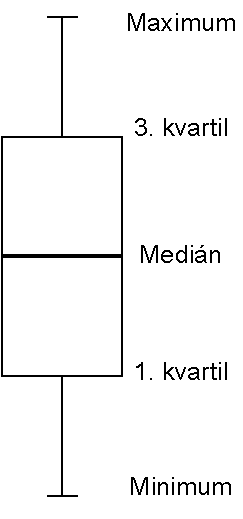
\includegraphics[width=0.25\textwidth]{obrazky-figures/box_plot.pdf}
	\caption{Důležité kvantily, které lze pomocí krabicového grafu zkoumat.}
	\label{box_plot}
\end{figure}


\subsection*{Houslový graf}

Houslový graf zobrazuje podobně jako krabicový graf významné kvantily daného atributu. Navíc ale přidává i zobrazení odhadu hustoty pravděpodobnosti. Je vhodný zejména pro data, která se řídí multimodální distribucí\footnote{Distribuce, která má dva nebo více lokálních maxim.}, protože uživatel získá oproti krabicovému grafu výrazně lepší představu o opravdovém rozložení dat \cite{violin_plot}. Porovnání krabicového a houslového grafu je vyobrazeno na obrázku \ref{box_violin_plots}.


\begin{figure}[h]%
    \centering
    \begin{subfigure}{\textwidth}
        \centering
        \resizebox{1\textwidth}{!}
        {
            %% Creator: Matplotlib, PGF backend
%%
%% To include the figure in your LaTeX document, write
%%   \input{<filename>.pgf}
%%
%% Make sure the required packages are loaded in your preamble
%%   \usepackage{pgf}
%%
%% Also ensure that all the required font packages are loaded; for instance,
%% the lmodern package is sometimes necessary when using math font.
%%   \usepackage{lmodern}
%%
%% Figures using additional raster images can only be included by \input if
%% they are in the same directory as the main LaTeX file. For loading figures
%% from other directories you can use the `import` package
%%   \usepackage{import}
%%
%% and then include the figures with
%%   \import{<path to file>}{<filename>.pgf}
%%
%% Matplotlib used the following preamble
%%   \usepackage{fontspec}
%%   \setmainfont{DejaVuSerif.ttf}[Path=\detokenize{/home/ankimme/fit/ibt/env/lib/python3.10/site-packages/matplotlib/mpl-data/fonts/ttf/}]
%%   \setsansfont{DejaVuSans.ttf}[Path=\detokenize{/home/ankimme/fit/ibt/env/lib/python3.10/site-packages/matplotlib/mpl-data/fonts/ttf/}]
%%   \setmonofont{DejaVuSansMono.ttf}[Path=\detokenize{/home/ankimme/fit/ibt/env/lib/python3.10/site-packages/matplotlib/mpl-data/fonts/ttf/}]
%%
\begingroup%
\makeatletter%
\begin{pgfpicture}%
\pgfpathrectangle{\pgfpointorigin}{\pgfqpoint{9.000000in}{3.000000in}}%
\pgfusepath{use as bounding box, clip}%
\begin{pgfscope}%
\pgfsetbuttcap%
\pgfsetmiterjoin%
\pgfsetlinewidth{0.000000pt}%
\definecolor{currentstroke}{rgb}{1.000000,1.000000,1.000000}%
\pgfsetstrokecolor{currentstroke}%
\pgfsetstrokeopacity{0.000000}%
\pgfsetdash{}{0pt}%
\pgfpathmoveto{\pgfqpoint{0.000000in}{0.000000in}}%
\pgfpathlineto{\pgfqpoint{9.000000in}{0.000000in}}%
\pgfpathlineto{\pgfqpoint{9.000000in}{3.000000in}}%
\pgfpathlineto{\pgfqpoint{0.000000in}{3.000000in}}%
\pgfpathlineto{\pgfqpoint{0.000000in}{0.000000in}}%
\pgfpathclose%
\pgfusepath{}%
\end{pgfscope}%
\begin{pgfscope}%
\pgfsetbuttcap%
\pgfsetmiterjoin%
\definecolor{currentfill}{rgb}{1.000000,1.000000,1.000000}%
\pgfsetfillcolor{currentfill}%
\pgfsetlinewidth{0.000000pt}%
\definecolor{currentstroke}{rgb}{0.000000,0.000000,0.000000}%
\pgfsetstrokecolor{currentstroke}%
\pgfsetstrokeopacity{0.000000}%
\pgfsetdash{}{0pt}%
\pgfpathmoveto{\pgfqpoint{0.571835in}{0.327070in}}%
\pgfpathlineto{\pgfqpoint{8.958330in}{0.327070in}}%
\pgfpathlineto{\pgfqpoint{8.958330in}{2.958330in}}%
\pgfpathlineto{\pgfqpoint{0.571835in}{2.958330in}}%
\pgfpathlineto{\pgfqpoint{0.571835in}{0.327070in}}%
\pgfpathclose%
\pgfusepath{fill}%
\end{pgfscope}%
\begin{pgfscope}%
\pgfpathrectangle{\pgfqpoint{0.571835in}{0.327070in}}{\pgfqpoint{8.386495in}{2.631260in}}%
\pgfusepath{clip}%
\pgfsetbuttcap%
\pgfsetmiterjoin%
\definecolor{currentfill}{rgb}{0.121569,0.466667,0.705882}%
\pgfsetfillcolor{currentfill}%
\pgfsetfillopacity{0.400000}%
\pgfsetlinewidth{0.000000pt}%
\definecolor{currentstroke}{rgb}{0.000000,0.000000,0.000000}%
\pgfsetstrokecolor{currentstroke}%
\pgfsetstrokeopacity{0.400000}%
\pgfsetdash{}{0pt}%
\pgfpathmoveto{\pgfqpoint{1.530937in}{0.327070in}}%
\pgfpathlineto{\pgfqpoint{1.721181in}{0.327070in}}%
\pgfpathlineto{\pgfqpoint{1.721181in}{0.337745in}}%
\pgfpathlineto{\pgfqpoint{1.530937in}{0.337745in}}%
\pgfpathlineto{\pgfqpoint{1.530937in}{0.327070in}}%
\pgfpathclose%
\pgfusepath{fill}%
\end{pgfscope}%
\begin{pgfscope}%
\pgfpathrectangle{\pgfqpoint{0.571835in}{0.327070in}}{\pgfqpoint{8.386495in}{2.631260in}}%
\pgfusepath{clip}%
\pgfsetbuttcap%
\pgfsetmiterjoin%
\definecolor{currentfill}{rgb}{0.121569,0.466667,0.705882}%
\pgfsetfillcolor{currentfill}%
\pgfsetfillopacity{0.400000}%
\pgfsetlinewidth{0.000000pt}%
\definecolor{currentstroke}{rgb}{0.000000,0.000000,0.000000}%
\pgfsetstrokecolor{currentstroke}%
\pgfsetstrokeopacity{0.400000}%
\pgfsetdash{}{0pt}%
\pgfpathmoveto{\pgfqpoint{1.721181in}{0.327070in}}%
\pgfpathlineto{\pgfqpoint{1.911425in}{0.327070in}}%
\pgfpathlineto{\pgfqpoint{1.911425in}{0.332408in}}%
\pgfpathlineto{\pgfqpoint{1.721181in}{0.332408in}}%
\pgfpathlineto{\pgfqpoint{1.721181in}{0.327070in}}%
\pgfpathclose%
\pgfusepath{fill}%
\end{pgfscope}%
\begin{pgfscope}%
\pgfpathrectangle{\pgfqpoint{0.571835in}{0.327070in}}{\pgfqpoint{8.386495in}{2.631260in}}%
\pgfusepath{clip}%
\pgfsetbuttcap%
\pgfsetmiterjoin%
\definecolor{currentfill}{rgb}{0.121569,0.466667,0.705882}%
\pgfsetfillcolor{currentfill}%
\pgfsetfillopacity{0.400000}%
\pgfsetlinewidth{0.000000pt}%
\definecolor{currentstroke}{rgb}{0.000000,0.000000,0.000000}%
\pgfsetstrokecolor{currentstroke}%
\pgfsetstrokeopacity{0.400000}%
\pgfsetdash{}{0pt}%
\pgfpathmoveto{\pgfqpoint{1.911425in}{0.327070in}}%
\pgfpathlineto{\pgfqpoint{2.101669in}{0.327070in}}%
\pgfpathlineto{\pgfqpoint{2.101669in}{0.332408in}}%
\pgfpathlineto{\pgfqpoint{1.911425in}{0.332408in}}%
\pgfpathlineto{\pgfqpoint{1.911425in}{0.327070in}}%
\pgfpathclose%
\pgfusepath{fill}%
\end{pgfscope}%
\begin{pgfscope}%
\pgfpathrectangle{\pgfqpoint{0.571835in}{0.327070in}}{\pgfqpoint{8.386495in}{2.631260in}}%
\pgfusepath{clip}%
\pgfsetbuttcap%
\pgfsetmiterjoin%
\definecolor{currentfill}{rgb}{0.121569,0.466667,0.705882}%
\pgfsetfillcolor{currentfill}%
\pgfsetfillopacity{0.400000}%
\pgfsetlinewidth{0.000000pt}%
\definecolor{currentstroke}{rgb}{0.000000,0.000000,0.000000}%
\pgfsetstrokecolor{currentstroke}%
\pgfsetstrokeopacity{0.400000}%
\pgfsetdash{}{0pt}%
\pgfpathmoveto{\pgfqpoint{2.101669in}{0.327070in}}%
\pgfpathlineto{\pgfqpoint{2.291912in}{0.327070in}}%
\pgfpathlineto{\pgfqpoint{2.291912in}{0.345752in}}%
\pgfpathlineto{\pgfqpoint{2.101669in}{0.345752in}}%
\pgfpathlineto{\pgfqpoint{2.101669in}{0.327070in}}%
\pgfpathclose%
\pgfusepath{fill}%
\end{pgfscope}%
\begin{pgfscope}%
\pgfpathrectangle{\pgfqpoint{0.571835in}{0.327070in}}{\pgfqpoint{8.386495in}{2.631260in}}%
\pgfusepath{clip}%
\pgfsetbuttcap%
\pgfsetmiterjoin%
\definecolor{currentfill}{rgb}{0.121569,0.466667,0.705882}%
\pgfsetfillcolor{currentfill}%
\pgfsetfillopacity{0.400000}%
\pgfsetlinewidth{0.000000pt}%
\definecolor{currentstroke}{rgb}{0.000000,0.000000,0.000000}%
\pgfsetstrokecolor{currentstroke}%
\pgfsetstrokeopacity{0.400000}%
\pgfsetdash{}{0pt}%
\pgfpathmoveto{\pgfqpoint{2.291912in}{0.327070in}}%
\pgfpathlineto{\pgfqpoint{2.482156in}{0.327070in}}%
\pgfpathlineto{\pgfqpoint{2.482156in}{0.369770in}}%
\pgfpathlineto{\pgfqpoint{2.291912in}{0.369770in}}%
\pgfpathlineto{\pgfqpoint{2.291912in}{0.327070in}}%
\pgfpathclose%
\pgfusepath{fill}%
\end{pgfscope}%
\begin{pgfscope}%
\pgfpathrectangle{\pgfqpoint{0.571835in}{0.327070in}}{\pgfqpoint{8.386495in}{2.631260in}}%
\pgfusepath{clip}%
\pgfsetbuttcap%
\pgfsetmiterjoin%
\definecolor{currentfill}{rgb}{0.121569,0.466667,0.705882}%
\pgfsetfillcolor{currentfill}%
\pgfsetfillopacity{0.400000}%
\pgfsetlinewidth{0.000000pt}%
\definecolor{currentstroke}{rgb}{0.000000,0.000000,0.000000}%
\pgfsetstrokecolor{currentstroke}%
\pgfsetstrokeopacity{0.400000}%
\pgfsetdash{}{0pt}%
\pgfpathmoveto{\pgfqpoint{2.482156in}{0.327070in}}%
\pgfpathlineto{\pgfqpoint{2.672400in}{0.327070in}}%
\pgfpathlineto{\pgfqpoint{2.672400in}{0.399127in}}%
\pgfpathlineto{\pgfqpoint{2.482156in}{0.399127in}}%
\pgfpathlineto{\pgfqpoint{2.482156in}{0.327070in}}%
\pgfpathclose%
\pgfusepath{fill}%
\end{pgfscope}%
\begin{pgfscope}%
\pgfpathrectangle{\pgfqpoint{0.571835in}{0.327070in}}{\pgfqpoint{8.386495in}{2.631260in}}%
\pgfusepath{clip}%
\pgfsetbuttcap%
\pgfsetmiterjoin%
\definecolor{currentfill}{rgb}{0.121569,0.466667,0.705882}%
\pgfsetfillcolor{currentfill}%
\pgfsetfillopacity{0.400000}%
\pgfsetlinewidth{0.000000pt}%
\definecolor{currentstroke}{rgb}{0.000000,0.000000,0.000000}%
\pgfsetstrokecolor{currentstroke}%
\pgfsetstrokeopacity{0.400000}%
\pgfsetdash{}{0pt}%
\pgfpathmoveto{\pgfqpoint{2.672400in}{0.327070in}}%
\pgfpathlineto{\pgfqpoint{2.862644in}{0.327070in}}%
\pgfpathlineto{\pgfqpoint{2.862644in}{0.436489in}}%
\pgfpathlineto{\pgfqpoint{2.672400in}{0.436489in}}%
\pgfpathlineto{\pgfqpoint{2.672400in}{0.327070in}}%
\pgfpathclose%
\pgfusepath{fill}%
\end{pgfscope}%
\begin{pgfscope}%
\pgfpathrectangle{\pgfqpoint{0.571835in}{0.327070in}}{\pgfqpoint{8.386495in}{2.631260in}}%
\pgfusepath{clip}%
\pgfsetbuttcap%
\pgfsetmiterjoin%
\definecolor{currentfill}{rgb}{0.121569,0.466667,0.705882}%
\pgfsetfillcolor{currentfill}%
\pgfsetfillopacity{0.400000}%
\pgfsetlinewidth{0.000000pt}%
\definecolor{currentstroke}{rgb}{0.000000,0.000000,0.000000}%
\pgfsetstrokecolor{currentstroke}%
\pgfsetstrokeopacity{0.400000}%
\pgfsetdash{}{0pt}%
\pgfpathmoveto{\pgfqpoint{2.862644in}{0.327070in}}%
\pgfpathlineto{\pgfqpoint{3.052888in}{0.327070in}}%
\pgfpathlineto{\pgfqpoint{3.052888in}{0.511214in}}%
\pgfpathlineto{\pgfqpoint{2.862644in}{0.511214in}}%
\pgfpathlineto{\pgfqpoint{2.862644in}{0.327070in}}%
\pgfpathclose%
\pgfusepath{fill}%
\end{pgfscope}%
\begin{pgfscope}%
\pgfpathrectangle{\pgfqpoint{0.571835in}{0.327070in}}{\pgfqpoint{8.386495in}{2.631260in}}%
\pgfusepath{clip}%
\pgfsetbuttcap%
\pgfsetmiterjoin%
\definecolor{currentfill}{rgb}{0.121569,0.466667,0.705882}%
\pgfsetfillcolor{currentfill}%
\pgfsetfillopacity{0.400000}%
\pgfsetlinewidth{0.000000pt}%
\definecolor{currentstroke}{rgb}{0.000000,0.000000,0.000000}%
\pgfsetstrokecolor{currentstroke}%
\pgfsetstrokeopacity{0.400000}%
\pgfsetdash{}{0pt}%
\pgfpathmoveto{\pgfqpoint{3.052888in}{0.327070in}}%
\pgfpathlineto{\pgfqpoint{3.243132in}{0.327070in}}%
\pgfpathlineto{\pgfqpoint{3.243132in}{0.617965in}}%
\pgfpathlineto{\pgfqpoint{3.052888in}{0.617965in}}%
\pgfpathlineto{\pgfqpoint{3.052888in}{0.327070in}}%
\pgfpathclose%
\pgfusepath{fill}%
\end{pgfscope}%
\begin{pgfscope}%
\pgfpathrectangle{\pgfqpoint{0.571835in}{0.327070in}}{\pgfqpoint{8.386495in}{2.631260in}}%
\pgfusepath{clip}%
\pgfsetbuttcap%
\pgfsetmiterjoin%
\definecolor{currentfill}{rgb}{0.121569,0.466667,0.705882}%
\pgfsetfillcolor{currentfill}%
\pgfsetfillopacity{0.400000}%
\pgfsetlinewidth{0.000000pt}%
\definecolor{currentstroke}{rgb}{0.000000,0.000000,0.000000}%
\pgfsetstrokecolor{currentstroke}%
\pgfsetstrokeopacity{0.400000}%
\pgfsetdash{}{0pt}%
\pgfpathmoveto{\pgfqpoint{3.243132in}{0.327070in}}%
\pgfpathlineto{\pgfqpoint{3.433376in}{0.327070in}}%
\pgfpathlineto{\pgfqpoint{3.433376in}{0.719377in}}%
\pgfpathlineto{\pgfqpoint{3.243132in}{0.719377in}}%
\pgfpathlineto{\pgfqpoint{3.243132in}{0.327070in}}%
\pgfpathclose%
\pgfusepath{fill}%
\end{pgfscope}%
\begin{pgfscope}%
\pgfpathrectangle{\pgfqpoint{0.571835in}{0.327070in}}{\pgfqpoint{8.386495in}{2.631260in}}%
\pgfusepath{clip}%
\pgfsetbuttcap%
\pgfsetmiterjoin%
\definecolor{currentfill}{rgb}{0.121569,0.466667,0.705882}%
\pgfsetfillcolor{currentfill}%
\pgfsetfillopacity{0.400000}%
\pgfsetlinewidth{0.000000pt}%
\definecolor{currentstroke}{rgb}{0.000000,0.000000,0.000000}%
\pgfsetstrokecolor{currentstroke}%
\pgfsetstrokeopacity{0.400000}%
\pgfsetdash{}{0pt}%
\pgfpathmoveto{\pgfqpoint{3.433376in}{0.327070in}}%
\pgfpathlineto{\pgfqpoint{3.623619in}{0.327070in}}%
\pgfpathlineto{\pgfqpoint{3.623619in}{0.892846in}}%
\pgfpathlineto{\pgfqpoint{3.433376in}{0.892846in}}%
\pgfpathlineto{\pgfqpoint{3.433376in}{0.327070in}}%
\pgfpathclose%
\pgfusepath{fill}%
\end{pgfscope}%
\begin{pgfscope}%
\pgfpathrectangle{\pgfqpoint{0.571835in}{0.327070in}}{\pgfqpoint{8.386495in}{2.631260in}}%
\pgfusepath{clip}%
\pgfsetbuttcap%
\pgfsetmiterjoin%
\definecolor{currentfill}{rgb}{0.121569,0.466667,0.705882}%
\pgfsetfillcolor{currentfill}%
\pgfsetfillopacity{0.400000}%
\pgfsetlinewidth{0.000000pt}%
\definecolor{currentstroke}{rgb}{0.000000,0.000000,0.000000}%
\pgfsetstrokecolor{currentstroke}%
\pgfsetstrokeopacity{0.400000}%
\pgfsetdash{}{0pt}%
\pgfpathmoveto{\pgfqpoint{3.623619in}{0.327070in}}%
\pgfpathlineto{\pgfqpoint{3.813863in}{0.327070in}}%
\pgfpathlineto{\pgfqpoint{3.813863in}{1.068984in}}%
\pgfpathlineto{\pgfqpoint{3.623619in}{1.068984in}}%
\pgfpathlineto{\pgfqpoint{3.623619in}{0.327070in}}%
\pgfpathclose%
\pgfusepath{fill}%
\end{pgfscope}%
\begin{pgfscope}%
\pgfpathrectangle{\pgfqpoint{0.571835in}{0.327070in}}{\pgfqpoint{8.386495in}{2.631260in}}%
\pgfusepath{clip}%
\pgfsetbuttcap%
\pgfsetmiterjoin%
\definecolor{currentfill}{rgb}{0.121569,0.466667,0.705882}%
\pgfsetfillcolor{currentfill}%
\pgfsetfillopacity{0.400000}%
\pgfsetlinewidth{0.000000pt}%
\definecolor{currentstroke}{rgb}{0.000000,0.000000,0.000000}%
\pgfsetstrokecolor{currentstroke}%
\pgfsetstrokeopacity{0.400000}%
\pgfsetdash{}{0pt}%
\pgfpathmoveto{\pgfqpoint{3.813863in}{0.327070in}}%
\pgfpathlineto{\pgfqpoint{4.004107in}{0.327070in}}%
\pgfpathlineto{\pgfqpoint{4.004107in}{1.263804in}}%
\pgfpathlineto{\pgfqpoint{3.813863in}{1.263804in}}%
\pgfpathlineto{\pgfqpoint{3.813863in}{0.327070in}}%
\pgfpathclose%
\pgfusepath{fill}%
\end{pgfscope}%
\begin{pgfscope}%
\pgfpathrectangle{\pgfqpoint{0.571835in}{0.327070in}}{\pgfqpoint{8.386495in}{2.631260in}}%
\pgfusepath{clip}%
\pgfsetbuttcap%
\pgfsetmiterjoin%
\definecolor{currentfill}{rgb}{0.121569,0.466667,0.705882}%
\pgfsetfillcolor{currentfill}%
\pgfsetfillopacity{0.400000}%
\pgfsetlinewidth{0.000000pt}%
\definecolor{currentstroke}{rgb}{0.000000,0.000000,0.000000}%
\pgfsetstrokecolor{currentstroke}%
\pgfsetstrokeopacity{0.400000}%
\pgfsetdash{}{0pt}%
\pgfpathmoveto{\pgfqpoint{4.004107in}{0.327070in}}%
\pgfpathlineto{\pgfqpoint{4.194351in}{0.327070in}}%
\pgfpathlineto{\pgfqpoint{4.194351in}{1.402579in}}%
\pgfpathlineto{\pgfqpoint{4.004107in}{1.402579in}}%
\pgfpathlineto{\pgfqpoint{4.004107in}{0.327070in}}%
\pgfpathclose%
\pgfusepath{fill}%
\end{pgfscope}%
\begin{pgfscope}%
\pgfpathrectangle{\pgfqpoint{0.571835in}{0.327070in}}{\pgfqpoint{8.386495in}{2.631260in}}%
\pgfusepath{clip}%
\pgfsetbuttcap%
\pgfsetmiterjoin%
\definecolor{currentfill}{rgb}{0.121569,0.466667,0.705882}%
\pgfsetfillcolor{currentfill}%
\pgfsetfillopacity{0.400000}%
\pgfsetlinewidth{0.000000pt}%
\definecolor{currentstroke}{rgb}{0.000000,0.000000,0.000000}%
\pgfsetstrokecolor{currentstroke}%
\pgfsetstrokeopacity{0.400000}%
\pgfsetdash{}{0pt}%
\pgfpathmoveto{\pgfqpoint{4.194351in}{0.327070in}}%
\pgfpathlineto{\pgfqpoint{4.384595in}{0.327070in}}%
\pgfpathlineto{\pgfqpoint{4.384595in}{1.426598in}}%
\pgfpathlineto{\pgfqpoint{4.194351in}{1.426598in}}%
\pgfpathlineto{\pgfqpoint{4.194351in}{0.327070in}}%
\pgfpathclose%
\pgfusepath{fill}%
\end{pgfscope}%
\begin{pgfscope}%
\pgfpathrectangle{\pgfqpoint{0.571835in}{0.327070in}}{\pgfqpoint{8.386495in}{2.631260in}}%
\pgfusepath{clip}%
\pgfsetbuttcap%
\pgfsetmiterjoin%
\definecolor{currentfill}{rgb}{0.121569,0.466667,0.705882}%
\pgfsetfillcolor{currentfill}%
\pgfsetfillopacity{0.400000}%
\pgfsetlinewidth{0.000000pt}%
\definecolor{currentstroke}{rgb}{0.000000,0.000000,0.000000}%
\pgfsetstrokecolor{currentstroke}%
\pgfsetstrokeopacity{0.400000}%
\pgfsetdash{}{0pt}%
\pgfpathmoveto{\pgfqpoint{4.384595in}{0.327070in}}%
\pgfpathlineto{\pgfqpoint{4.574839in}{0.327070in}}%
\pgfpathlineto{\pgfqpoint{4.574839in}{1.565373in}}%
\pgfpathlineto{\pgfqpoint{4.384595in}{1.565373in}}%
\pgfpathlineto{\pgfqpoint{4.384595in}{0.327070in}}%
\pgfpathclose%
\pgfusepath{fill}%
\end{pgfscope}%
\begin{pgfscope}%
\pgfpathrectangle{\pgfqpoint{0.571835in}{0.327070in}}{\pgfqpoint{8.386495in}{2.631260in}}%
\pgfusepath{clip}%
\pgfsetbuttcap%
\pgfsetmiterjoin%
\definecolor{currentfill}{rgb}{0.121569,0.466667,0.705882}%
\pgfsetfillcolor{currentfill}%
\pgfsetfillopacity{0.400000}%
\pgfsetlinewidth{0.000000pt}%
\definecolor{currentstroke}{rgb}{0.000000,0.000000,0.000000}%
\pgfsetstrokecolor{currentstroke}%
\pgfsetstrokeopacity{0.400000}%
\pgfsetdash{}{0pt}%
\pgfpathmoveto{\pgfqpoint{4.574839in}{0.327070in}}%
\pgfpathlineto{\pgfqpoint{4.765082in}{0.327070in}}%
\pgfpathlineto{\pgfqpoint{4.765082in}{1.471966in}}%
\pgfpathlineto{\pgfqpoint{4.574839in}{1.471966in}}%
\pgfpathlineto{\pgfqpoint{4.574839in}{0.327070in}}%
\pgfpathclose%
\pgfusepath{fill}%
\end{pgfscope}%
\begin{pgfscope}%
\pgfpathrectangle{\pgfqpoint{0.571835in}{0.327070in}}{\pgfqpoint{8.386495in}{2.631260in}}%
\pgfusepath{clip}%
\pgfsetbuttcap%
\pgfsetmiterjoin%
\definecolor{currentfill}{rgb}{0.121569,0.466667,0.705882}%
\pgfsetfillcolor{currentfill}%
\pgfsetfillopacity{0.400000}%
\pgfsetlinewidth{0.000000pt}%
\definecolor{currentstroke}{rgb}{0.000000,0.000000,0.000000}%
\pgfsetstrokecolor{currentstroke}%
\pgfsetstrokeopacity{0.400000}%
\pgfsetdash{}{0pt}%
\pgfpathmoveto{\pgfqpoint{4.765082in}{0.327070in}}%
\pgfpathlineto{\pgfqpoint{4.955326in}{0.327070in}}%
\pgfpathlineto{\pgfqpoint{4.955326in}{1.455954in}}%
\pgfpathlineto{\pgfqpoint{4.765082in}{1.455954in}}%
\pgfpathlineto{\pgfqpoint{4.765082in}{0.327070in}}%
\pgfpathclose%
\pgfusepath{fill}%
\end{pgfscope}%
\begin{pgfscope}%
\pgfpathrectangle{\pgfqpoint{0.571835in}{0.327070in}}{\pgfqpoint{8.386495in}{2.631260in}}%
\pgfusepath{clip}%
\pgfsetbuttcap%
\pgfsetmiterjoin%
\definecolor{currentfill}{rgb}{0.121569,0.466667,0.705882}%
\pgfsetfillcolor{currentfill}%
\pgfsetfillopacity{0.400000}%
\pgfsetlinewidth{0.000000pt}%
\definecolor{currentstroke}{rgb}{0.000000,0.000000,0.000000}%
\pgfsetstrokecolor{currentstroke}%
\pgfsetstrokeopacity{0.400000}%
\pgfsetdash{}{0pt}%
\pgfpathmoveto{\pgfqpoint{4.955326in}{0.327070in}}%
\pgfpathlineto{\pgfqpoint{5.145570in}{0.327070in}}%
\pgfpathlineto{\pgfqpoint{5.145570in}{1.351872in}}%
\pgfpathlineto{\pgfqpoint{4.955326in}{1.351872in}}%
\pgfpathlineto{\pgfqpoint{4.955326in}{0.327070in}}%
\pgfpathclose%
\pgfusepath{fill}%
\end{pgfscope}%
\begin{pgfscope}%
\pgfpathrectangle{\pgfqpoint{0.571835in}{0.327070in}}{\pgfqpoint{8.386495in}{2.631260in}}%
\pgfusepath{clip}%
\pgfsetbuttcap%
\pgfsetmiterjoin%
\definecolor{currentfill}{rgb}{0.121569,0.466667,0.705882}%
\pgfsetfillcolor{currentfill}%
\pgfsetfillopacity{0.400000}%
\pgfsetlinewidth{0.000000pt}%
\definecolor{currentstroke}{rgb}{0.000000,0.000000,0.000000}%
\pgfsetstrokecolor{currentstroke}%
\pgfsetstrokeopacity{0.400000}%
\pgfsetdash{}{0pt}%
\pgfpathmoveto{\pgfqpoint{5.145570in}{0.327070in}}%
\pgfpathlineto{\pgfqpoint{5.335814in}{0.327070in}}%
\pgfpathlineto{\pgfqpoint{5.335814in}{1.173066in}}%
\pgfpathlineto{\pgfqpoint{5.145570in}{1.173066in}}%
\pgfpathlineto{\pgfqpoint{5.145570in}{0.327070in}}%
\pgfpathclose%
\pgfusepath{fill}%
\end{pgfscope}%
\begin{pgfscope}%
\pgfpathrectangle{\pgfqpoint{0.571835in}{0.327070in}}{\pgfqpoint{8.386495in}{2.631260in}}%
\pgfusepath{clip}%
\pgfsetbuttcap%
\pgfsetmiterjoin%
\definecolor{currentfill}{rgb}{0.121569,0.466667,0.705882}%
\pgfsetfillcolor{currentfill}%
\pgfsetfillopacity{0.400000}%
\pgfsetlinewidth{0.000000pt}%
\definecolor{currentstroke}{rgb}{0.000000,0.000000,0.000000}%
\pgfsetstrokecolor{currentstroke}%
\pgfsetstrokeopacity{0.400000}%
\pgfsetdash{}{0pt}%
\pgfpathmoveto{\pgfqpoint{5.335814in}{0.327070in}}%
\pgfpathlineto{\pgfqpoint{5.526058in}{0.327070in}}%
\pgfpathlineto{\pgfqpoint{5.526058in}{1.084997in}}%
\pgfpathlineto{\pgfqpoint{5.335814in}{1.084997in}}%
\pgfpathlineto{\pgfqpoint{5.335814in}{0.327070in}}%
\pgfpathclose%
\pgfusepath{fill}%
\end{pgfscope}%
\begin{pgfscope}%
\pgfpathrectangle{\pgfqpoint{0.571835in}{0.327070in}}{\pgfqpoint{8.386495in}{2.631260in}}%
\pgfusepath{clip}%
\pgfsetbuttcap%
\pgfsetmiterjoin%
\definecolor{currentfill}{rgb}{0.121569,0.466667,0.705882}%
\pgfsetfillcolor{currentfill}%
\pgfsetfillopacity{0.400000}%
\pgfsetlinewidth{0.000000pt}%
\definecolor{currentstroke}{rgb}{0.000000,0.000000,0.000000}%
\pgfsetstrokecolor{currentstroke}%
\pgfsetstrokeopacity{0.400000}%
\pgfsetdash{}{0pt}%
\pgfpathmoveto{\pgfqpoint{5.526058in}{0.327070in}}%
\pgfpathlineto{\pgfqpoint{5.716302in}{0.327070in}}%
\pgfpathlineto{\pgfqpoint{5.716302in}{1.018278in}}%
\pgfpathlineto{\pgfqpoint{5.526058in}{1.018278in}}%
\pgfpathlineto{\pgfqpoint{5.526058in}{0.327070in}}%
\pgfpathclose%
\pgfusepath{fill}%
\end{pgfscope}%
\begin{pgfscope}%
\pgfpathrectangle{\pgfqpoint{0.571835in}{0.327070in}}{\pgfqpoint{8.386495in}{2.631260in}}%
\pgfusepath{clip}%
\pgfsetbuttcap%
\pgfsetmiterjoin%
\definecolor{currentfill}{rgb}{0.121569,0.466667,0.705882}%
\pgfsetfillcolor{currentfill}%
\pgfsetfillopacity{0.400000}%
\pgfsetlinewidth{0.000000pt}%
\definecolor{currentstroke}{rgb}{0.000000,0.000000,0.000000}%
\pgfsetstrokecolor{currentstroke}%
\pgfsetstrokeopacity{0.400000}%
\pgfsetdash{}{0pt}%
\pgfpathmoveto{\pgfqpoint{5.716302in}{0.327070in}}%
\pgfpathlineto{\pgfqpoint{5.906546in}{0.327070in}}%
\pgfpathlineto{\pgfqpoint{5.906546in}{1.103678in}}%
\pgfpathlineto{\pgfqpoint{5.716302in}{1.103678in}}%
\pgfpathlineto{\pgfqpoint{5.716302in}{0.327070in}}%
\pgfpathclose%
\pgfusepath{fill}%
\end{pgfscope}%
\begin{pgfscope}%
\pgfpathrectangle{\pgfqpoint{0.571835in}{0.327070in}}{\pgfqpoint{8.386495in}{2.631260in}}%
\pgfusepath{clip}%
\pgfsetbuttcap%
\pgfsetmiterjoin%
\definecolor{currentfill}{rgb}{0.121569,0.466667,0.705882}%
\pgfsetfillcolor{currentfill}%
\pgfsetfillopacity{0.400000}%
\pgfsetlinewidth{0.000000pt}%
\definecolor{currentstroke}{rgb}{0.000000,0.000000,0.000000}%
\pgfsetstrokecolor{currentstroke}%
\pgfsetstrokeopacity{0.400000}%
\pgfsetdash{}{0pt}%
\pgfpathmoveto{\pgfqpoint{5.906546in}{0.327070in}}%
\pgfpathlineto{\pgfqpoint{6.096789in}{0.327070in}}%
\pgfpathlineto{\pgfqpoint{6.096789in}{1.522673in}}%
\pgfpathlineto{\pgfqpoint{5.906546in}{1.522673in}}%
\pgfpathlineto{\pgfqpoint{5.906546in}{0.327070in}}%
\pgfpathclose%
\pgfusepath{fill}%
\end{pgfscope}%
\begin{pgfscope}%
\pgfpathrectangle{\pgfqpoint{0.571835in}{0.327070in}}{\pgfqpoint{8.386495in}{2.631260in}}%
\pgfusepath{clip}%
\pgfsetbuttcap%
\pgfsetmiterjoin%
\definecolor{currentfill}{rgb}{0.121569,0.466667,0.705882}%
\pgfsetfillcolor{currentfill}%
\pgfsetfillopacity{0.400000}%
\pgfsetlinewidth{0.000000pt}%
\definecolor{currentstroke}{rgb}{0.000000,0.000000,0.000000}%
\pgfsetstrokecolor{currentstroke}%
\pgfsetstrokeopacity{0.400000}%
\pgfsetdash{}{0pt}%
\pgfpathmoveto{\pgfqpoint{6.096789in}{0.327070in}}%
\pgfpathlineto{\pgfqpoint{6.287033in}{0.327070in}}%
\pgfpathlineto{\pgfqpoint{6.287033in}{2.011055in}}%
\pgfpathlineto{\pgfqpoint{6.096789in}{2.011055in}}%
\pgfpathlineto{\pgfqpoint{6.096789in}{0.327070in}}%
\pgfpathclose%
\pgfusepath{fill}%
\end{pgfscope}%
\begin{pgfscope}%
\pgfpathrectangle{\pgfqpoint{0.571835in}{0.327070in}}{\pgfqpoint{8.386495in}{2.631260in}}%
\pgfusepath{clip}%
\pgfsetbuttcap%
\pgfsetmiterjoin%
\definecolor{currentfill}{rgb}{0.121569,0.466667,0.705882}%
\pgfsetfillcolor{currentfill}%
\pgfsetfillopacity{0.400000}%
\pgfsetlinewidth{0.000000pt}%
\definecolor{currentstroke}{rgb}{0.000000,0.000000,0.000000}%
\pgfsetstrokecolor{currentstroke}%
\pgfsetstrokeopacity{0.400000}%
\pgfsetdash{}{0pt}%
\pgfpathmoveto{\pgfqpoint{6.287033in}{0.327070in}}%
\pgfpathlineto{\pgfqpoint{6.477277in}{0.327070in}}%
\pgfpathlineto{\pgfqpoint{6.477277in}{2.504775in}}%
\pgfpathlineto{\pgfqpoint{6.287033in}{2.504775in}}%
\pgfpathlineto{\pgfqpoint{6.287033in}{0.327070in}}%
\pgfpathclose%
\pgfusepath{fill}%
\end{pgfscope}%
\begin{pgfscope}%
\pgfpathrectangle{\pgfqpoint{0.571835in}{0.327070in}}{\pgfqpoint{8.386495in}{2.631260in}}%
\pgfusepath{clip}%
\pgfsetbuttcap%
\pgfsetmiterjoin%
\definecolor{currentfill}{rgb}{0.121569,0.466667,0.705882}%
\pgfsetfillcolor{currentfill}%
\pgfsetfillopacity{0.400000}%
\pgfsetlinewidth{0.000000pt}%
\definecolor{currentstroke}{rgb}{0.000000,0.000000,0.000000}%
\pgfsetstrokecolor{currentstroke}%
\pgfsetstrokeopacity{0.400000}%
\pgfsetdash{}{0pt}%
\pgfpathmoveto{\pgfqpoint{6.477277in}{0.327070in}}%
\pgfpathlineto{\pgfqpoint{6.667521in}{0.327070in}}%
\pgfpathlineto{\pgfqpoint{6.667521in}{2.833032in}}%
\pgfpathlineto{\pgfqpoint{6.477277in}{2.833032in}}%
\pgfpathlineto{\pgfqpoint{6.477277in}{0.327070in}}%
\pgfpathclose%
\pgfusepath{fill}%
\end{pgfscope}%
\begin{pgfscope}%
\pgfpathrectangle{\pgfqpoint{0.571835in}{0.327070in}}{\pgfqpoint{8.386495in}{2.631260in}}%
\pgfusepath{clip}%
\pgfsetbuttcap%
\pgfsetmiterjoin%
\definecolor{currentfill}{rgb}{0.121569,0.466667,0.705882}%
\pgfsetfillcolor{currentfill}%
\pgfsetfillopacity{0.400000}%
\pgfsetlinewidth{0.000000pt}%
\definecolor{currentstroke}{rgb}{0.000000,0.000000,0.000000}%
\pgfsetstrokecolor{currentstroke}%
\pgfsetstrokeopacity{0.400000}%
\pgfsetdash{}{0pt}%
\pgfpathmoveto{\pgfqpoint{6.667521in}{0.327070in}}%
\pgfpathlineto{\pgfqpoint{6.857765in}{0.327070in}}%
\pgfpathlineto{\pgfqpoint{6.857765in}{2.592844in}}%
\pgfpathlineto{\pgfqpoint{6.667521in}{2.592844in}}%
\pgfpathlineto{\pgfqpoint{6.667521in}{0.327070in}}%
\pgfpathclose%
\pgfusepath{fill}%
\end{pgfscope}%
\begin{pgfscope}%
\pgfpathrectangle{\pgfqpoint{0.571835in}{0.327070in}}{\pgfqpoint{8.386495in}{2.631260in}}%
\pgfusepath{clip}%
\pgfsetbuttcap%
\pgfsetmiterjoin%
\definecolor{currentfill}{rgb}{0.121569,0.466667,0.705882}%
\pgfsetfillcolor{currentfill}%
\pgfsetfillopacity{0.400000}%
\pgfsetlinewidth{0.000000pt}%
\definecolor{currentstroke}{rgb}{0.000000,0.000000,0.000000}%
\pgfsetstrokecolor{currentstroke}%
\pgfsetstrokeopacity{0.400000}%
\pgfsetdash{}{0pt}%
\pgfpathmoveto{\pgfqpoint{6.857765in}{0.327070in}}%
\pgfpathlineto{\pgfqpoint{7.048009in}{0.327070in}}%
\pgfpathlineto{\pgfqpoint{7.048009in}{2.085780in}}%
\pgfpathlineto{\pgfqpoint{6.857765in}{2.085780in}}%
\pgfpathlineto{\pgfqpoint{6.857765in}{0.327070in}}%
\pgfpathclose%
\pgfusepath{fill}%
\end{pgfscope}%
\begin{pgfscope}%
\pgfpathrectangle{\pgfqpoint{0.571835in}{0.327070in}}{\pgfqpoint{8.386495in}{2.631260in}}%
\pgfusepath{clip}%
\pgfsetbuttcap%
\pgfsetmiterjoin%
\definecolor{currentfill}{rgb}{0.121569,0.466667,0.705882}%
\pgfsetfillcolor{currentfill}%
\pgfsetfillopacity{0.400000}%
\pgfsetlinewidth{0.000000pt}%
\definecolor{currentstroke}{rgb}{0.000000,0.000000,0.000000}%
\pgfsetstrokecolor{currentstroke}%
\pgfsetstrokeopacity{0.400000}%
\pgfsetdash{}{0pt}%
\pgfpathmoveto{\pgfqpoint{7.048009in}{0.327070in}}%
\pgfpathlineto{\pgfqpoint{7.238253in}{0.327070in}}%
\pgfpathlineto{\pgfqpoint{7.238253in}{1.410585in}}%
\pgfpathlineto{\pgfqpoint{7.048009in}{1.410585in}}%
\pgfpathlineto{\pgfqpoint{7.048009in}{0.327070in}}%
\pgfpathclose%
\pgfusepath{fill}%
\end{pgfscope}%
\begin{pgfscope}%
\pgfpathrectangle{\pgfqpoint{0.571835in}{0.327070in}}{\pgfqpoint{8.386495in}{2.631260in}}%
\pgfusepath{clip}%
\pgfsetbuttcap%
\pgfsetmiterjoin%
\definecolor{currentfill}{rgb}{0.121569,0.466667,0.705882}%
\pgfsetfillcolor{currentfill}%
\pgfsetfillopacity{0.400000}%
\pgfsetlinewidth{0.000000pt}%
\definecolor{currentstroke}{rgb}{0.000000,0.000000,0.000000}%
\pgfsetstrokecolor{currentstroke}%
\pgfsetstrokeopacity{0.400000}%
\pgfsetdash{}{0pt}%
\pgfpathmoveto{\pgfqpoint{7.238253in}{0.327070in}}%
\pgfpathlineto{\pgfqpoint{7.428496in}{0.327070in}}%
\pgfpathlineto{\pgfqpoint{7.428496in}{0.866159in}}%
\pgfpathlineto{\pgfqpoint{7.238253in}{0.866159in}}%
\pgfpathlineto{\pgfqpoint{7.238253in}{0.327070in}}%
\pgfpathclose%
\pgfusepath{fill}%
\end{pgfscope}%
\begin{pgfscope}%
\pgfpathrectangle{\pgfqpoint{0.571835in}{0.327070in}}{\pgfqpoint{8.386495in}{2.631260in}}%
\pgfusepath{clip}%
\pgfsetbuttcap%
\pgfsetmiterjoin%
\definecolor{currentfill}{rgb}{0.121569,0.466667,0.705882}%
\pgfsetfillcolor{currentfill}%
\pgfsetfillopacity{0.400000}%
\pgfsetlinewidth{0.000000pt}%
\definecolor{currentstroke}{rgb}{0.000000,0.000000,0.000000}%
\pgfsetstrokecolor{currentstroke}%
\pgfsetstrokeopacity{0.400000}%
\pgfsetdash{}{0pt}%
\pgfpathmoveto{\pgfqpoint{7.428496in}{0.327070in}}%
\pgfpathlineto{\pgfqpoint{7.618740in}{0.327070in}}%
\pgfpathlineto{\pgfqpoint{7.618740in}{0.524558in}}%
\pgfpathlineto{\pgfqpoint{7.428496in}{0.524558in}}%
\pgfpathlineto{\pgfqpoint{7.428496in}{0.327070in}}%
\pgfpathclose%
\pgfusepath{fill}%
\end{pgfscope}%
\begin{pgfscope}%
\pgfpathrectangle{\pgfqpoint{0.571835in}{0.327070in}}{\pgfqpoint{8.386495in}{2.631260in}}%
\pgfusepath{clip}%
\pgfsetbuttcap%
\pgfsetmiterjoin%
\definecolor{currentfill}{rgb}{0.121569,0.466667,0.705882}%
\pgfsetfillcolor{currentfill}%
\pgfsetfillopacity{0.400000}%
\pgfsetlinewidth{0.000000pt}%
\definecolor{currentstroke}{rgb}{0.000000,0.000000,0.000000}%
\pgfsetstrokecolor{currentstroke}%
\pgfsetstrokeopacity{0.400000}%
\pgfsetdash{}{0pt}%
\pgfpathmoveto{\pgfqpoint{7.618740in}{0.327070in}}%
\pgfpathlineto{\pgfqpoint{7.808984in}{0.327070in}}%
\pgfpathlineto{\pgfqpoint{7.808984in}{0.423145in}}%
\pgfpathlineto{\pgfqpoint{7.618740in}{0.423145in}}%
\pgfpathlineto{\pgfqpoint{7.618740in}{0.327070in}}%
\pgfpathclose%
\pgfusepath{fill}%
\end{pgfscope}%
\begin{pgfscope}%
\pgfpathrectangle{\pgfqpoint{0.571835in}{0.327070in}}{\pgfqpoint{8.386495in}{2.631260in}}%
\pgfusepath{clip}%
\pgfsetbuttcap%
\pgfsetmiterjoin%
\definecolor{currentfill}{rgb}{0.121569,0.466667,0.705882}%
\pgfsetfillcolor{currentfill}%
\pgfsetfillopacity{0.400000}%
\pgfsetlinewidth{0.000000pt}%
\definecolor{currentstroke}{rgb}{0.000000,0.000000,0.000000}%
\pgfsetstrokecolor{currentstroke}%
\pgfsetstrokeopacity{0.400000}%
\pgfsetdash{}{0pt}%
\pgfpathmoveto{\pgfqpoint{7.808984in}{0.327070in}}%
\pgfpathlineto{\pgfqpoint{7.999228in}{0.327070in}}%
\pgfpathlineto{\pgfqpoint{7.999228in}{0.351089in}}%
\pgfpathlineto{\pgfqpoint{7.808984in}{0.351089in}}%
\pgfpathlineto{\pgfqpoint{7.808984in}{0.327070in}}%
\pgfpathclose%
\pgfusepath{fill}%
\end{pgfscope}%
\begin{pgfscope}%
\pgfsetbuttcap%
\pgfsetroundjoin%
\definecolor{currentfill}{rgb}{0.000000,0.000000,0.000000}%
\pgfsetfillcolor{currentfill}%
\pgfsetlinewidth{0.803000pt}%
\definecolor{currentstroke}{rgb}{0.000000,0.000000,0.000000}%
\pgfsetstrokecolor{currentstroke}%
\pgfsetdash{}{0pt}%
\pgfsys@defobject{currentmarker}{\pgfqpoint{0.000000in}{-0.048611in}}{\pgfqpoint{0.000000in}{0.000000in}}{%
\pgfpathmoveto{\pgfqpoint{0.000000in}{0.000000in}}%
\pgfpathlineto{\pgfqpoint{0.000000in}{-0.048611in}}%
\pgfusepath{stroke,fill}%
}%
\begin{pgfscope}%
\pgfsys@transformshift{1.274709in}{0.327070in}%
\pgfsys@useobject{currentmarker}{}%
\end{pgfscope}%
\end{pgfscope}%
\begin{pgfscope}%
\definecolor{textcolor}{rgb}{0.000000,0.000000,0.000000}%
\pgfsetstrokecolor{textcolor}%
\pgfsetfillcolor{textcolor}%
\pgftext[x=1.274709in,y=0.229848in,,top]{\color{textcolor}\sffamily\fontsize{14.000000}{16.800000}\selectfont \ensuremath{-}10.0}%
\end{pgfscope}%
\begin{pgfscope}%
\pgfsetbuttcap%
\pgfsetroundjoin%
\definecolor{currentfill}{rgb}{0.000000,0.000000,0.000000}%
\pgfsetfillcolor{currentfill}%
\pgfsetlinewidth{0.803000pt}%
\definecolor{currentstroke}{rgb}{0.000000,0.000000,0.000000}%
\pgfsetstrokecolor{currentstroke}%
\pgfsetdash{}{0pt}%
\pgfsys@defobject{currentmarker}{\pgfqpoint{0.000000in}{-0.048611in}}{\pgfqpoint{0.000000in}{0.000000in}}{%
\pgfpathmoveto{\pgfqpoint{0.000000in}{0.000000in}}%
\pgfpathlineto{\pgfqpoint{0.000000in}{-0.048611in}}%
\pgfusepath{stroke,fill}%
}%
\begin{pgfscope}%
\pgfsys@transformshift{2.302374in}{0.327070in}%
\pgfsys@useobject{currentmarker}{}%
\end{pgfscope}%
\end{pgfscope}%
\begin{pgfscope}%
\definecolor{textcolor}{rgb}{0.000000,0.000000,0.000000}%
\pgfsetstrokecolor{textcolor}%
\pgfsetfillcolor{textcolor}%
\pgftext[x=2.302374in,y=0.229848in,,top]{\color{textcolor}\sffamily\fontsize{14.000000}{16.800000}\selectfont \ensuremath{-}7.5}%
\end{pgfscope}%
\begin{pgfscope}%
\pgfsetbuttcap%
\pgfsetroundjoin%
\definecolor{currentfill}{rgb}{0.000000,0.000000,0.000000}%
\pgfsetfillcolor{currentfill}%
\pgfsetlinewidth{0.803000pt}%
\definecolor{currentstroke}{rgb}{0.000000,0.000000,0.000000}%
\pgfsetstrokecolor{currentstroke}%
\pgfsetdash{}{0pt}%
\pgfsys@defobject{currentmarker}{\pgfqpoint{0.000000in}{-0.048611in}}{\pgfqpoint{0.000000in}{0.000000in}}{%
\pgfpathmoveto{\pgfqpoint{0.000000in}{0.000000in}}%
\pgfpathlineto{\pgfqpoint{0.000000in}{-0.048611in}}%
\pgfusepath{stroke,fill}%
}%
\begin{pgfscope}%
\pgfsys@transformshift{3.330040in}{0.327070in}%
\pgfsys@useobject{currentmarker}{}%
\end{pgfscope}%
\end{pgfscope}%
\begin{pgfscope}%
\definecolor{textcolor}{rgb}{0.000000,0.000000,0.000000}%
\pgfsetstrokecolor{textcolor}%
\pgfsetfillcolor{textcolor}%
\pgftext[x=3.330040in,y=0.229848in,,top]{\color{textcolor}\sffamily\fontsize{14.000000}{16.800000}\selectfont \ensuremath{-}5.0}%
\end{pgfscope}%
\begin{pgfscope}%
\pgfsetbuttcap%
\pgfsetroundjoin%
\definecolor{currentfill}{rgb}{0.000000,0.000000,0.000000}%
\pgfsetfillcolor{currentfill}%
\pgfsetlinewidth{0.803000pt}%
\definecolor{currentstroke}{rgb}{0.000000,0.000000,0.000000}%
\pgfsetstrokecolor{currentstroke}%
\pgfsetdash{}{0pt}%
\pgfsys@defobject{currentmarker}{\pgfqpoint{0.000000in}{-0.048611in}}{\pgfqpoint{0.000000in}{0.000000in}}{%
\pgfpathmoveto{\pgfqpoint{0.000000in}{0.000000in}}%
\pgfpathlineto{\pgfqpoint{0.000000in}{-0.048611in}}%
\pgfusepath{stroke,fill}%
}%
\begin{pgfscope}%
\pgfsys@transformshift{4.357706in}{0.327070in}%
\pgfsys@useobject{currentmarker}{}%
\end{pgfscope}%
\end{pgfscope}%
\begin{pgfscope}%
\definecolor{textcolor}{rgb}{0.000000,0.000000,0.000000}%
\pgfsetstrokecolor{textcolor}%
\pgfsetfillcolor{textcolor}%
\pgftext[x=4.357706in,y=0.229848in,,top]{\color{textcolor}\sffamily\fontsize{14.000000}{16.800000}\selectfont \ensuremath{-}2.5}%
\end{pgfscope}%
\begin{pgfscope}%
\pgfsetbuttcap%
\pgfsetroundjoin%
\definecolor{currentfill}{rgb}{0.000000,0.000000,0.000000}%
\pgfsetfillcolor{currentfill}%
\pgfsetlinewidth{0.803000pt}%
\definecolor{currentstroke}{rgb}{0.000000,0.000000,0.000000}%
\pgfsetstrokecolor{currentstroke}%
\pgfsetdash{}{0pt}%
\pgfsys@defobject{currentmarker}{\pgfqpoint{0.000000in}{-0.048611in}}{\pgfqpoint{0.000000in}{0.000000in}}{%
\pgfpathmoveto{\pgfqpoint{0.000000in}{0.000000in}}%
\pgfpathlineto{\pgfqpoint{0.000000in}{-0.048611in}}%
\pgfusepath{stroke,fill}%
}%
\begin{pgfscope}%
\pgfsys@transformshift{5.385371in}{0.327070in}%
\pgfsys@useobject{currentmarker}{}%
\end{pgfscope}%
\end{pgfscope}%
\begin{pgfscope}%
\definecolor{textcolor}{rgb}{0.000000,0.000000,0.000000}%
\pgfsetstrokecolor{textcolor}%
\pgfsetfillcolor{textcolor}%
\pgftext[x=5.385371in,y=0.229848in,,top]{\color{textcolor}\sffamily\fontsize{14.000000}{16.800000}\selectfont 0.0}%
\end{pgfscope}%
\begin{pgfscope}%
\pgfsetbuttcap%
\pgfsetroundjoin%
\definecolor{currentfill}{rgb}{0.000000,0.000000,0.000000}%
\pgfsetfillcolor{currentfill}%
\pgfsetlinewidth{0.803000pt}%
\definecolor{currentstroke}{rgb}{0.000000,0.000000,0.000000}%
\pgfsetstrokecolor{currentstroke}%
\pgfsetdash{}{0pt}%
\pgfsys@defobject{currentmarker}{\pgfqpoint{0.000000in}{-0.048611in}}{\pgfqpoint{0.000000in}{0.000000in}}{%
\pgfpathmoveto{\pgfqpoint{0.000000in}{0.000000in}}%
\pgfpathlineto{\pgfqpoint{0.000000in}{-0.048611in}}%
\pgfusepath{stroke,fill}%
}%
\begin{pgfscope}%
\pgfsys@transformshift{6.413037in}{0.327070in}%
\pgfsys@useobject{currentmarker}{}%
\end{pgfscope}%
\end{pgfscope}%
\begin{pgfscope}%
\definecolor{textcolor}{rgb}{0.000000,0.000000,0.000000}%
\pgfsetstrokecolor{textcolor}%
\pgfsetfillcolor{textcolor}%
\pgftext[x=6.413037in,y=0.229848in,,top]{\color{textcolor}\sffamily\fontsize{14.000000}{16.800000}\selectfont 2.5}%
\end{pgfscope}%
\begin{pgfscope}%
\pgfsetbuttcap%
\pgfsetroundjoin%
\definecolor{currentfill}{rgb}{0.000000,0.000000,0.000000}%
\pgfsetfillcolor{currentfill}%
\pgfsetlinewidth{0.803000pt}%
\definecolor{currentstroke}{rgb}{0.000000,0.000000,0.000000}%
\pgfsetstrokecolor{currentstroke}%
\pgfsetdash{}{0pt}%
\pgfsys@defobject{currentmarker}{\pgfqpoint{0.000000in}{-0.048611in}}{\pgfqpoint{0.000000in}{0.000000in}}{%
\pgfpathmoveto{\pgfqpoint{0.000000in}{0.000000in}}%
\pgfpathlineto{\pgfqpoint{0.000000in}{-0.048611in}}%
\pgfusepath{stroke,fill}%
}%
\begin{pgfscope}%
\pgfsys@transformshift{7.440702in}{0.327070in}%
\pgfsys@useobject{currentmarker}{}%
\end{pgfscope}%
\end{pgfscope}%
\begin{pgfscope}%
\definecolor{textcolor}{rgb}{0.000000,0.000000,0.000000}%
\pgfsetstrokecolor{textcolor}%
\pgfsetfillcolor{textcolor}%
\pgftext[x=7.440702in,y=0.229848in,,top]{\color{textcolor}\sffamily\fontsize{14.000000}{16.800000}\selectfont 5.0}%
\end{pgfscope}%
\begin{pgfscope}%
\pgfsetbuttcap%
\pgfsetroundjoin%
\definecolor{currentfill}{rgb}{0.000000,0.000000,0.000000}%
\pgfsetfillcolor{currentfill}%
\pgfsetlinewidth{0.803000pt}%
\definecolor{currentstroke}{rgb}{0.000000,0.000000,0.000000}%
\pgfsetstrokecolor{currentstroke}%
\pgfsetdash{}{0pt}%
\pgfsys@defobject{currentmarker}{\pgfqpoint{0.000000in}{-0.048611in}}{\pgfqpoint{0.000000in}{0.000000in}}{%
\pgfpathmoveto{\pgfqpoint{0.000000in}{0.000000in}}%
\pgfpathlineto{\pgfqpoint{0.000000in}{-0.048611in}}%
\pgfusepath{stroke,fill}%
}%
\begin{pgfscope}%
\pgfsys@transformshift{8.468368in}{0.327070in}%
\pgfsys@useobject{currentmarker}{}%
\end{pgfscope}%
\end{pgfscope}%
\begin{pgfscope}%
\definecolor{textcolor}{rgb}{0.000000,0.000000,0.000000}%
\pgfsetstrokecolor{textcolor}%
\pgfsetfillcolor{textcolor}%
\pgftext[x=8.468368in,y=0.229848in,,top]{\color{textcolor}\sffamily\fontsize{14.000000}{16.800000}\selectfont 7.5}%
\end{pgfscope}%
\begin{pgfscope}%
\pgfsetbuttcap%
\pgfsetroundjoin%
\definecolor{currentfill}{rgb}{0.000000,0.000000,0.000000}%
\pgfsetfillcolor{currentfill}%
\pgfsetlinewidth{0.803000pt}%
\definecolor{currentstroke}{rgb}{0.000000,0.000000,0.000000}%
\pgfsetstrokecolor{currentstroke}%
\pgfsetdash{}{0pt}%
\pgfsys@defobject{currentmarker}{\pgfqpoint{-0.048611in}{0.000000in}}{\pgfqpoint{-0.000000in}{0.000000in}}{%
\pgfpathmoveto{\pgfqpoint{-0.000000in}{0.000000in}}%
\pgfpathlineto{\pgfqpoint{-0.048611in}{0.000000in}}%
\pgfusepath{stroke,fill}%
}%
\begin{pgfscope}%
\pgfsys@transformshift{0.571835in}{0.327070in}%
\pgfsys@useobject{currentmarker}{}%
\end{pgfscope}%
\end{pgfscope}%
\begin{pgfscope}%
\definecolor{textcolor}{rgb}{0.000000,0.000000,0.000000}%
\pgfsetstrokecolor{textcolor}%
\pgfsetfillcolor{textcolor}%
\pgftext[x=0.041670in, y=0.253204in, left, base]{\color{textcolor}\sffamily\fontsize{14.000000}{16.800000}\selectfont 0.00}%
\end{pgfscope}%
\begin{pgfscope}%
\pgfsetbuttcap%
\pgfsetroundjoin%
\definecolor{currentfill}{rgb}{0.000000,0.000000,0.000000}%
\pgfsetfillcolor{currentfill}%
\pgfsetlinewidth{0.803000pt}%
\definecolor{currentstroke}{rgb}{0.000000,0.000000,0.000000}%
\pgfsetstrokecolor{currentstroke}%
\pgfsetdash{}{0pt}%
\pgfsys@defobject{currentmarker}{\pgfqpoint{-0.048611in}{0.000000in}}{\pgfqpoint{-0.000000in}{0.000000in}}{%
\pgfpathmoveto{\pgfqpoint{-0.000000in}{0.000000in}}%
\pgfpathlineto{\pgfqpoint{-0.048611in}{0.000000in}}%
\pgfusepath{stroke,fill}%
}%
\begin{pgfscope}%
\pgfsys@transformshift{0.571835in}{0.944628in}%
\pgfsys@useobject{currentmarker}{}%
\end{pgfscope}%
\end{pgfscope}%
\begin{pgfscope}%
\definecolor{textcolor}{rgb}{0.000000,0.000000,0.000000}%
\pgfsetstrokecolor{textcolor}%
\pgfsetfillcolor{textcolor}%
\pgftext[x=0.041670in, y=0.870762in, left, base]{\color{textcolor}\sffamily\fontsize{14.000000}{16.800000}\selectfont 0.05}%
\end{pgfscope}%
\begin{pgfscope}%
\pgfsetbuttcap%
\pgfsetroundjoin%
\definecolor{currentfill}{rgb}{0.000000,0.000000,0.000000}%
\pgfsetfillcolor{currentfill}%
\pgfsetlinewidth{0.803000pt}%
\definecolor{currentstroke}{rgb}{0.000000,0.000000,0.000000}%
\pgfsetstrokecolor{currentstroke}%
\pgfsetdash{}{0pt}%
\pgfsys@defobject{currentmarker}{\pgfqpoint{-0.048611in}{0.000000in}}{\pgfqpoint{-0.000000in}{0.000000in}}{%
\pgfpathmoveto{\pgfqpoint{-0.000000in}{0.000000in}}%
\pgfpathlineto{\pgfqpoint{-0.048611in}{0.000000in}}%
\pgfusepath{stroke,fill}%
}%
\begin{pgfscope}%
\pgfsys@transformshift{0.571835in}{1.562186in}%
\pgfsys@useobject{currentmarker}{}%
\end{pgfscope}%
\end{pgfscope}%
\begin{pgfscope}%
\definecolor{textcolor}{rgb}{0.000000,0.000000,0.000000}%
\pgfsetstrokecolor{textcolor}%
\pgfsetfillcolor{textcolor}%
\pgftext[x=0.041670in, y=1.488320in, left, base]{\color{textcolor}\sffamily\fontsize{14.000000}{16.800000}\selectfont 0.10}%
\end{pgfscope}%
\begin{pgfscope}%
\pgfsetbuttcap%
\pgfsetroundjoin%
\definecolor{currentfill}{rgb}{0.000000,0.000000,0.000000}%
\pgfsetfillcolor{currentfill}%
\pgfsetlinewidth{0.803000pt}%
\definecolor{currentstroke}{rgb}{0.000000,0.000000,0.000000}%
\pgfsetstrokecolor{currentstroke}%
\pgfsetdash{}{0pt}%
\pgfsys@defobject{currentmarker}{\pgfqpoint{-0.048611in}{0.000000in}}{\pgfqpoint{-0.000000in}{0.000000in}}{%
\pgfpathmoveto{\pgfqpoint{-0.000000in}{0.000000in}}%
\pgfpathlineto{\pgfqpoint{-0.048611in}{0.000000in}}%
\pgfusepath{stroke,fill}%
}%
\begin{pgfscope}%
\pgfsys@transformshift{0.571835in}{2.179744in}%
\pgfsys@useobject{currentmarker}{}%
\end{pgfscope}%
\end{pgfscope}%
\begin{pgfscope}%
\definecolor{textcolor}{rgb}{0.000000,0.000000,0.000000}%
\pgfsetstrokecolor{textcolor}%
\pgfsetfillcolor{textcolor}%
\pgftext[x=0.041670in, y=2.105878in, left, base]{\color{textcolor}\sffamily\fontsize{14.000000}{16.800000}\selectfont 0.15}%
\end{pgfscope}%
\begin{pgfscope}%
\pgfsetbuttcap%
\pgfsetroundjoin%
\definecolor{currentfill}{rgb}{0.000000,0.000000,0.000000}%
\pgfsetfillcolor{currentfill}%
\pgfsetlinewidth{0.803000pt}%
\definecolor{currentstroke}{rgb}{0.000000,0.000000,0.000000}%
\pgfsetstrokecolor{currentstroke}%
\pgfsetdash{}{0pt}%
\pgfsys@defobject{currentmarker}{\pgfqpoint{-0.048611in}{0.000000in}}{\pgfqpoint{-0.000000in}{0.000000in}}{%
\pgfpathmoveto{\pgfqpoint{-0.000000in}{0.000000in}}%
\pgfpathlineto{\pgfqpoint{-0.048611in}{0.000000in}}%
\pgfusepath{stroke,fill}%
}%
\begin{pgfscope}%
\pgfsys@transformshift{0.571835in}{2.797302in}%
\pgfsys@useobject{currentmarker}{}%
\end{pgfscope}%
\end{pgfscope}%
\begin{pgfscope}%
\definecolor{textcolor}{rgb}{0.000000,0.000000,0.000000}%
\pgfsetstrokecolor{textcolor}%
\pgfsetfillcolor{textcolor}%
\pgftext[x=0.041670in, y=2.723435in, left, base]{\color{textcolor}\sffamily\fontsize{14.000000}{16.800000}\selectfont 0.20}%
\end{pgfscope}%
\begin{pgfscope}%
\pgfpathrectangle{\pgfqpoint{0.571835in}{0.327070in}}{\pgfqpoint{8.386495in}{2.631260in}}%
\pgfusepath{clip}%
\pgfsetrectcap%
\pgfsetroundjoin%
\pgfsetlinewidth{1.505625pt}%
\definecolor{currentstroke}{rgb}{0.121569,0.466667,0.705882}%
\pgfsetstrokecolor{currentstroke}%
\pgfsetdash{}{0pt}%
\pgfpathmoveto{\pgfqpoint{0.953039in}{0.327090in}}%
\pgfpathlineto{\pgfqpoint{1.297847in}{0.328403in}}%
\pgfpathlineto{\pgfqpoint{1.987463in}{0.337398in}}%
\pgfpathlineto{\pgfqpoint{2.102399in}{0.342649in}}%
\pgfpathlineto{\pgfqpoint{2.217335in}{0.351037in}}%
\pgfpathlineto{\pgfqpoint{2.332271in}{0.362853in}}%
\pgfpathlineto{\pgfqpoint{2.447207in}{0.378756in}}%
\pgfpathlineto{\pgfqpoint{2.523831in}{0.392230in}}%
\pgfpathlineto{\pgfqpoint{2.600455in}{0.408512in}}%
\pgfpathlineto{\pgfqpoint{2.677079in}{0.427910in}}%
\pgfpathlineto{\pgfqpoint{2.753703in}{0.450496in}}%
\pgfpathlineto{\pgfqpoint{2.830327in}{0.476181in}}%
\pgfpathlineto{\pgfqpoint{2.906951in}{0.505004in}}%
\pgfpathlineto{\pgfqpoint{2.983575in}{0.537359in}}%
\pgfpathlineto{\pgfqpoint{3.060199in}{0.573877in}}%
\pgfpathlineto{\pgfqpoint{3.136823in}{0.615067in}}%
\pgfpathlineto{\pgfqpoint{3.213447in}{0.661107in}}%
\pgfpathlineto{\pgfqpoint{3.290071in}{0.711994in}}%
\pgfpathlineto{\pgfqpoint{3.366695in}{0.767700in}}%
\pgfpathlineto{\pgfqpoint{3.443319in}{0.827997in}}%
\pgfpathlineto{\pgfqpoint{3.519943in}{0.892153in}}%
\pgfpathlineto{\pgfqpoint{3.634879in}{0.992938in}}%
\pgfpathlineto{\pgfqpoint{3.826439in}{1.162810in}}%
\pgfpathlineto{\pgfqpoint{3.903063in}{1.227809in}}%
\pgfpathlineto{\pgfqpoint{3.979687in}{1.288430in}}%
\pgfpathlineto{\pgfqpoint{4.017999in}{1.316341in}}%
\pgfpathlineto{\pgfqpoint{4.056311in}{1.342243in}}%
\pgfpathlineto{\pgfqpoint{4.094623in}{1.365888in}}%
\pgfpathlineto{\pgfqpoint{4.132935in}{1.387124in}}%
\pgfpathlineto{\pgfqpoint{4.171247in}{1.405935in}}%
\pgfpathlineto{\pgfqpoint{4.209559in}{1.422447in}}%
\pgfpathlineto{\pgfqpoint{4.247871in}{1.436905in}}%
\pgfpathlineto{\pgfqpoint{4.324495in}{1.460892in}}%
\pgfpathlineto{\pgfqpoint{4.401119in}{1.479759in}}%
\pgfpathlineto{\pgfqpoint{4.439431in}{1.487288in}}%
\pgfpathlineto{\pgfqpoint{4.477743in}{1.493242in}}%
\pgfpathlineto{\pgfqpoint{4.516055in}{1.497275in}}%
\pgfpathlineto{\pgfqpoint{4.554367in}{1.499032in}}%
\pgfpathlineto{\pgfqpoint{4.592679in}{1.498232in}}%
\pgfpathlineto{\pgfqpoint{4.630991in}{1.494716in}}%
\pgfpathlineto{\pgfqpoint{4.669303in}{1.488476in}}%
\pgfpathlineto{\pgfqpoint{4.707615in}{1.479647in}}%
\pgfpathlineto{\pgfqpoint{4.745927in}{1.468477in}}%
\pgfpathlineto{\pgfqpoint{4.784238in}{1.455287in}}%
\pgfpathlineto{\pgfqpoint{4.860862in}{1.424207in}}%
\pgfpathlineto{\pgfqpoint{4.937486in}{1.388705in}}%
\pgfpathlineto{\pgfqpoint{5.014110in}{1.349850in}}%
\pgfpathlineto{\pgfqpoint{5.090734in}{1.307509in}}%
\pgfpathlineto{\pgfqpoint{5.167358in}{1.261500in}}%
\pgfpathlineto{\pgfqpoint{5.320606in}{1.165571in}}%
\pgfpathlineto{\pgfqpoint{5.358918in}{1.143605in}}%
\pgfpathlineto{\pgfqpoint{5.397230in}{1.123679in}}%
\pgfpathlineto{\pgfqpoint{5.435542in}{1.106425in}}%
\pgfpathlineto{\pgfqpoint{5.473854in}{1.092475in}}%
\pgfpathlineto{\pgfqpoint{5.512166in}{1.082467in}}%
\pgfpathlineto{\pgfqpoint{5.550478in}{1.077073in}}%
\pgfpathlineto{\pgfqpoint{5.588790in}{1.077006in}}%
\pgfpathlineto{\pgfqpoint{5.627102in}{1.083020in}}%
\pgfpathlineto{\pgfqpoint{5.665414in}{1.095868in}}%
\pgfpathlineto{\pgfqpoint{5.703726in}{1.116259in}}%
\pgfpathlineto{\pgfqpoint{5.742038in}{1.144777in}}%
\pgfpathlineto{\pgfqpoint{5.780350in}{1.181821in}}%
\pgfpathlineto{\pgfqpoint{5.818662in}{1.227543in}}%
\pgfpathlineto{\pgfqpoint{5.856974in}{1.281822in}}%
\pgfpathlineto{\pgfqpoint{5.895286in}{1.344261in}}%
\pgfpathlineto{\pgfqpoint{5.933598in}{1.414213in}}%
\pgfpathlineto{\pgfqpoint{5.971910in}{1.490821in}}%
\pgfpathlineto{\pgfqpoint{6.010222in}{1.573075in}}%
\pgfpathlineto{\pgfqpoint{6.086846in}{1.749983in}}%
\pgfpathlineto{\pgfqpoint{6.240094in}{2.119116in}}%
\pgfpathlineto{\pgfqpoint{6.278406in}{2.207032in}}%
\pgfpathlineto{\pgfqpoint{6.316718in}{2.290372in}}%
\pgfpathlineto{\pgfqpoint{6.355030in}{2.367571in}}%
\pgfpathlineto{\pgfqpoint{6.393342in}{2.436996in}}%
\pgfpathlineto{\pgfqpoint{6.431654in}{2.496992in}}%
\pgfpathlineto{\pgfqpoint{6.469966in}{2.545961in}}%
\pgfpathlineto{\pgfqpoint{6.508278in}{2.582460in}}%
\pgfpathlineto{\pgfqpoint{6.546590in}{2.605300in}}%
\pgfpathlineto{\pgfqpoint{6.584902in}{2.613625in}}%
\pgfpathlineto{\pgfqpoint{6.623214in}{2.606971in}}%
\pgfpathlineto{\pgfqpoint{6.661526in}{2.585287in}}%
\pgfpathlineto{\pgfqpoint{6.699838in}{2.548919in}}%
\pgfpathlineto{\pgfqpoint{6.738150in}{2.498569in}}%
\pgfpathlineto{\pgfqpoint{6.776462in}{2.435245in}}%
\pgfpathlineto{\pgfqpoint{6.814774in}{2.360197in}}%
\pgfpathlineto{\pgfqpoint{6.853086in}{2.274860in}}%
\pgfpathlineto{\pgfqpoint{6.891398in}{2.180795in}}%
\pgfpathlineto{\pgfqpoint{6.929710in}{2.079641in}}%
\pgfpathlineto{\pgfqpoint{7.006334in}{1.862699in}}%
\pgfpathlineto{\pgfqpoint{7.159582in}{1.413407in}}%
\pgfpathlineto{\pgfqpoint{7.236206in}{1.201901in}}%
\pgfpathlineto{\pgfqpoint{7.274518in}{1.103132in}}%
\pgfpathlineto{\pgfqpoint{7.312830in}{1.010163in}}%
\pgfpathlineto{\pgfqpoint{7.351142in}{0.923708in}}%
\pgfpathlineto{\pgfqpoint{7.389454in}{0.844319in}}%
\pgfpathlineto{\pgfqpoint{7.427766in}{0.772354in}}%
\pgfpathlineto{\pgfqpoint{7.466078in}{0.707944in}}%
\pgfpathlineto{\pgfqpoint{7.504390in}{0.650983in}}%
\pgfpathlineto{\pgfqpoint{7.542702in}{0.601147in}}%
\pgfpathlineto{\pgfqpoint{7.581014in}{0.557930in}}%
\pgfpathlineto{\pgfqpoint{7.619326in}{0.520711in}}%
\pgfpathlineto{\pgfqpoint{7.657638in}{0.488810in}}%
\pgfpathlineto{\pgfqpoint{7.695950in}{0.461551in}}%
\pgfpathlineto{\pgfqpoint{7.734262in}{0.438307in}}%
\pgfpathlineto{\pgfqpoint{7.772574in}{0.418522in}}%
\pgfpathlineto{\pgfqpoint{7.810886in}{0.401721in}}%
\pgfpathlineto{\pgfqpoint{7.849198in}{0.387505in}}%
\pgfpathlineto{\pgfqpoint{7.887510in}{0.375537in}}%
\pgfpathlineto{\pgfqpoint{7.925822in}{0.365530in}}%
\pgfpathlineto{\pgfqpoint{8.002446in}{0.350419in}}%
\pgfpathlineto{\pgfqpoint{8.079070in}{0.340454in}}%
\pgfpathlineto{\pgfqpoint{8.155694in}{0.334225in}}%
\pgfpathlineto{\pgfqpoint{8.270630in}{0.329452in}}%
\pgfpathlineto{\pgfqpoint{8.423878in}{0.327449in}}%
\pgfpathlineto{\pgfqpoint{8.577126in}{0.327107in}}%
\pgfpathlineto{\pgfqpoint{8.577126in}{0.327107in}}%
\pgfusepath{stroke}%
\end{pgfscope}%
\begin{pgfscope}%
\pgfsetrectcap%
\pgfsetmiterjoin%
\pgfsetlinewidth{0.803000pt}%
\definecolor{currentstroke}{rgb}{0.000000,0.000000,0.000000}%
\pgfsetstrokecolor{currentstroke}%
\pgfsetdash{}{0pt}%
\pgfpathmoveto{\pgfqpoint{0.571835in}{0.327070in}}%
\pgfpathlineto{\pgfqpoint{0.571835in}{2.958330in}}%
\pgfusepath{stroke}%
\end{pgfscope}%
\begin{pgfscope}%
\pgfsetrectcap%
\pgfsetmiterjoin%
\pgfsetlinewidth{0.803000pt}%
\definecolor{currentstroke}{rgb}{0.000000,0.000000,0.000000}%
\pgfsetstrokecolor{currentstroke}%
\pgfsetdash{}{0pt}%
\pgfpathmoveto{\pgfqpoint{8.958330in}{0.327070in}}%
\pgfpathlineto{\pgfqpoint{8.958330in}{2.958330in}}%
\pgfusepath{stroke}%
\end{pgfscope}%
\begin{pgfscope}%
\pgfsetrectcap%
\pgfsetmiterjoin%
\pgfsetlinewidth{0.803000pt}%
\definecolor{currentstroke}{rgb}{0.000000,0.000000,0.000000}%
\pgfsetstrokecolor{currentstroke}%
\pgfsetdash{}{0pt}%
\pgfpathmoveto{\pgfqpoint{0.571835in}{0.327070in}}%
\pgfpathlineto{\pgfqpoint{8.958330in}{0.327070in}}%
\pgfusepath{stroke}%
\end{pgfscope}%
\begin{pgfscope}%
\pgfsetrectcap%
\pgfsetmiterjoin%
\pgfsetlinewidth{0.803000pt}%
\definecolor{currentstroke}{rgb}{0.000000,0.000000,0.000000}%
\pgfsetstrokecolor{currentstroke}%
\pgfsetdash{}{0pt}%
\pgfpathmoveto{\pgfqpoint{0.571835in}{2.958330in}}%
\pgfpathlineto{\pgfqpoint{8.958330in}{2.958330in}}%
\pgfusepath{stroke}%
\end{pgfscope}%
\end{pgfpicture}%
\makeatother%
\endgroup%

        }
        \captionsetup{width=.9\linewidth}
        \caption{Histogram dat řídící se bimodální distribucí. Distribuce vznikla spojením dvou normálních rozdělení s parametry $\mu=-2$, $\sigma=2$ a $\mu=3$, $\sigma=1$. Křivka znázorňuje odhad hustoty pravděpodobnosti.}
        \label{sub:violin_density}
    \end{subfigure}
    \par\medskip
    \begin{subfigure}{\textwidth}
        \centering
        \resizebox{1\textwidth}{!}
        {
            %% Creator: Matplotlib, PGF backend
%%
%% To include the figure in your LaTeX document, write
%%   \input{<filename>.pgf}
%%
%% Make sure the required packages are loaded in your preamble
%%   \usepackage{pgf}
%%
%% Also ensure that all the required font packages are loaded; for instance,
%% the lmodern package is sometimes necessary when using math font.
%%   \usepackage{lmodern}
%%
%% Figures using additional raster images can only be included by \input if
%% they are in the same directory as the main LaTeX file. For loading figures
%% from other directories you can use the `import` package
%%   \usepackage{import}
%%
%% and then include the figures with
%%   \import{<path to file>}{<filename>.pgf}
%%
%% Matplotlib used the following preamble
%%   \usepackage{fontspec}
%%   \setmainfont{DejaVuSerif.ttf}[Path=\detokenize{/home/ankimme/fit/ibt/env/lib/python3.10/site-packages/matplotlib/mpl-data/fonts/ttf/}]
%%   \setsansfont{DejaVuSans.ttf}[Path=\detokenize{/home/ankimme/fit/ibt/env/lib/python3.10/site-packages/matplotlib/mpl-data/fonts/ttf/}]
%%   \setmonofont{DejaVuSansMono.ttf}[Path=\detokenize{/home/ankimme/fit/ibt/env/lib/python3.10/site-packages/matplotlib/mpl-data/fonts/ttf/}]
%%
\begingroup%
\makeatletter%
\begin{pgfpicture}%
\pgfpathrectangle{\pgfpointorigin}{\pgfqpoint{9.000000in}{2.000000in}}%
\pgfusepath{use as bounding box, clip}%
\begin{pgfscope}%
\pgfsetbuttcap%
\pgfsetmiterjoin%
\pgfsetlinewidth{0.000000pt}%
\definecolor{currentstroke}{rgb}{1.000000,1.000000,1.000000}%
\pgfsetstrokecolor{currentstroke}%
\pgfsetstrokeopacity{0.000000}%
\pgfsetdash{}{0pt}%
\pgfpathmoveto{\pgfqpoint{0.000000in}{0.000000in}}%
\pgfpathlineto{\pgfqpoint{9.000000in}{0.000000in}}%
\pgfpathlineto{\pgfqpoint{9.000000in}{2.000000in}}%
\pgfpathlineto{\pgfqpoint{0.000000in}{2.000000in}}%
\pgfpathlineto{\pgfqpoint{0.000000in}{0.000000in}}%
\pgfpathclose%
\pgfusepath{}%
\end{pgfscope}%
\begin{pgfscope}%
\pgfsetbuttcap%
\pgfsetmiterjoin%
\definecolor{currentfill}{rgb}{1.000000,1.000000,1.000000}%
\pgfsetfillcolor{currentfill}%
\pgfsetlinewidth{0.000000pt}%
\definecolor{currentstroke}{rgb}{0.000000,0.000000,0.000000}%
\pgfsetstrokecolor{currentstroke}%
\pgfsetstrokeopacity{0.000000}%
\pgfsetdash{}{0pt}%
\pgfpathmoveto{\pgfqpoint{0.204343in}{0.327070in}}%
\pgfpathlineto{\pgfqpoint{8.958330in}{0.327070in}}%
\pgfpathlineto{\pgfqpoint{8.958330in}{1.958330in}}%
\pgfpathlineto{\pgfqpoint{0.204343in}{1.958330in}}%
\pgfpathlineto{\pgfqpoint{0.204343in}{0.327070in}}%
\pgfpathclose%
\pgfusepath{fill}%
\end{pgfscope}%
\begin{pgfscope}%
\pgfpathrectangle{\pgfqpoint{0.204343in}{0.327070in}}{\pgfqpoint{8.753987in}{1.631260in}}%
\pgfusepath{clip}%
\pgfsetbuttcap%
\pgfsetmiterjoin%
\definecolor{currentfill}{rgb}{0.194608,0.453431,0.632843}%
\pgfsetfillcolor{currentfill}%
\pgfsetlinewidth{1.505625pt}%
\definecolor{currentstroke}{rgb}{0.247059,0.247059,0.247059}%
\pgfsetstrokecolor{currentstroke}%
\pgfsetdash{}{0pt}%
\pgfpathmoveto{\pgfqpoint{4.265667in}{1.795204in}}%
\pgfpathlineto{\pgfqpoint{4.265667in}{0.490196in}}%
\pgfpathlineto{\pgfqpoint{6.751724in}{0.490196in}}%
\pgfpathlineto{\pgfqpoint{6.751724in}{1.795204in}}%
\pgfpathlineto{\pgfqpoint{4.265667in}{1.795204in}}%
\pgfpathlineto{\pgfqpoint{4.265667in}{1.795204in}}%
\pgfpathclose%
\pgfusepath{stroke,fill}%
\end{pgfscope}%
\begin{pgfscope}%
\pgfsetbuttcap%
\pgfsetroundjoin%
\definecolor{currentfill}{rgb}{0.000000,0.000000,0.000000}%
\pgfsetfillcolor{currentfill}%
\pgfsetlinewidth{0.803000pt}%
\definecolor{currentstroke}{rgb}{0.000000,0.000000,0.000000}%
\pgfsetstrokecolor{currentstroke}%
\pgfsetdash{}{0pt}%
\pgfsys@defobject{currentmarker}{\pgfqpoint{0.000000in}{-0.048611in}}{\pgfqpoint{0.000000in}{0.000000in}}{%
\pgfpathmoveto{\pgfqpoint{0.000000in}{0.000000in}}%
\pgfpathlineto{\pgfqpoint{0.000000in}{-0.048611in}}%
\pgfusepath{stroke,fill}%
}%
\begin{pgfscope}%
\pgfsys@transformshift{0.243194in}{0.327070in}%
\pgfsys@useobject{currentmarker}{}%
\end{pgfscope}%
\end{pgfscope}%
\begin{pgfscope}%
\definecolor{textcolor}{rgb}{0.000000,0.000000,0.000000}%
\pgfsetstrokecolor{textcolor}%
\pgfsetfillcolor{textcolor}%
\pgftext[x=0.243194in,y=0.229848in,,top]{\color{textcolor}\sffamily\fontsize{14.000000}{16.800000}\selectfont \ensuremath{-}10}%
\end{pgfscope}%
\begin{pgfscope}%
\pgfsetbuttcap%
\pgfsetroundjoin%
\definecolor{currentfill}{rgb}{0.000000,0.000000,0.000000}%
\pgfsetfillcolor{currentfill}%
\pgfsetlinewidth{0.803000pt}%
\definecolor{currentstroke}{rgb}{0.000000,0.000000,0.000000}%
\pgfsetstrokecolor{currentstroke}%
\pgfsetdash{}{0pt}%
\pgfsys@defobject{currentmarker}{\pgfqpoint{0.000000in}{-0.048611in}}{\pgfqpoint{0.000000in}{0.000000in}}{%
\pgfpathmoveto{\pgfqpoint{0.000000in}{0.000000in}}%
\pgfpathlineto{\pgfqpoint{0.000000in}{-0.048611in}}%
\pgfusepath{stroke,fill}%
}%
\begin{pgfscope}%
\pgfsys@transformshift{1.243970in}{0.327070in}%
\pgfsys@useobject{currentmarker}{}%
\end{pgfscope}%
\end{pgfscope}%
\begin{pgfscope}%
\definecolor{textcolor}{rgb}{0.000000,0.000000,0.000000}%
\pgfsetstrokecolor{textcolor}%
\pgfsetfillcolor{textcolor}%
\pgftext[x=1.243970in,y=0.229848in,,top]{\color{textcolor}\sffamily\fontsize{14.000000}{16.800000}\selectfont \ensuremath{-}8}%
\end{pgfscope}%
\begin{pgfscope}%
\pgfsetbuttcap%
\pgfsetroundjoin%
\definecolor{currentfill}{rgb}{0.000000,0.000000,0.000000}%
\pgfsetfillcolor{currentfill}%
\pgfsetlinewidth{0.803000pt}%
\definecolor{currentstroke}{rgb}{0.000000,0.000000,0.000000}%
\pgfsetstrokecolor{currentstroke}%
\pgfsetdash{}{0pt}%
\pgfsys@defobject{currentmarker}{\pgfqpoint{0.000000in}{-0.048611in}}{\pgfqpoint{0.000000in}{0.000000in}}{%
\pgfpathmoveto{\pgfqpoint{0.000000in}{0.000000in}}%
\pgfpathlineto{\pgfqpoint{0.000000in}{-0.048611in}}%
\pgfusepath{stroke,fill}%
}%
\begin{pgfscope}%
\pgfsys@transformshift{2.244746in}{0.327070in}%
\pgfsys@useobject{currentmarker}{}%
\end{pgfscope}%
\end{pgfscope}%
\begin{pgfscope}%
\definecolor{textcolor}{rgb}{0.000000,0.000000,0.000000}%
\pgfsetstrokecolor{textcolor}%
\pgfsetfillcolor{textcolor}%
\pgftext[x=2.244746in,y=0.229848in,,top]{\color{textcolor}\sffamily\fontsize{14.000000}{16.800000}\selectfont \ensuremath{-}6}%
\end{pgfscope}%
\begin{pgfscope}%
\pgfsetbuttcap%
\pgfsetroundjoin%
\definecolor{currentfill}{rgb}{0.000000,0.000000,0.000000}%
\pgfsetfillcolor{currentfill}%
\pgfsetlinewidth{0.803000pt}%
\definecolor{currentstroke}{rgb}{0.000000,0.000000,0.000000}%
\pgfsetstrokecolor{currentstroke}%
\pgfsetdash{}{0pt}%
\pgfsys@defobject{currentmarker}{\pgfqpoint{0.000000in}{-0.048611in}}{\pgfqpoint{0.000000in}{0.000000in}}{%
\pgfpathmoveto{\pgfqpoint{0.000000in}{0.000000in}}%
\pgfpathlineto{\pgfqpoint{0.000000in}{-0.048611in}}%
\pgfusepath{stroke,fill}%
}%
\begin{pgfscope}%
\pgfsys@transformshift{3.245522in}{0.327070in}%
\pgfsys@useobject{currentmarker}{}%
\end{pgfscope}%
\end{pgfscope}%
\begin{pgfscope}%
\definecolor{textcolor}{rgb}{0.000000,0.000000,0.000000}%
\pgfsetstrokecolor{textcolor}%
\pgfsetfillcolor{textcolor}%
\pgftext[x=3.245522in,y=0.229848in,,top]{\color{textcolor}\sffamily\fontsize{14.000000}{16.800000}\selectfont \ensuremath{-}4}%
\end{pgfscope}%
\begin{pgfscope}%
\pgfsetbuttcap%
\pgfsetroundjoin%
\definecolor{currentfill}{rgb}{0.000000,0.000000,0.000000}%
\pgfsetfillcolor{currentfill}%
\pgfsetlinewidth{0.803000pt}%
\definecolor{currentstroke}{rgb}{0.000000,0.000000,0.000000}%
\pgfsetstrokecolor{currentstroke}%
\pgfsetdash{}{0pt}%
\pgfsys@defobject{currentmarker}{\pgfqpoint{0.000000in}{-0.048611in}}{\pgfqpoint{0.000000in}{0.000000in}}{%
\pgfpathmoveto{\pgfqpoint{0.000000in}{0.000000in}}%
\pgfpathlineto{\pgfqpoint{0.000000in}{-0.048611in}}%
\pgfusepath{stroke,fill}%
}%
\begin{pgfscope}%
\pgfsys@transformshift{4.246298in}{0.327070in}%
\pgfsys@useobject{currentmarker}{}%
\end{pgfscope}%
\end{pgfscope}%
\begin{pgfscope}%
\definecolor{textcolor}{rgb}{0.000000,0.000000,0.000000}%
\pgfsetstrokecolor{textcolor}%
\pgfsetfillcolor{textcolor}%
\pgftext[x=4.246298in,y=0.229848in,,top]{\color{textcolor}\sffamily\fontsize{14.000000}{16.800000}\selectfont \ensuremath{-}2}%
\end{pgfscope}%
\begin{pgfscope}%
\pgfsetbuttcap%
\pgfsetroundjoin%
\definecolor{currentfill}{rgb}{0.000000,0.000000,0.000000}%
\pgfsetfillcolor{currentfill}%
\pgfsetlinewidth{0.803000pt}%
\definecolor{currentstroke}{rgb}{0.000000,0.000000,0.000000}%
\pgfsetstrokecolor{currentstroke}%
\pgfsetdash{}{0pt}%
\pgfsys@defobject{currentmarker}{\pgfqpoint{0.000000in}{-0.048611in}}{\pgfqpoint{0.000000in}{0.000000in}}{%
\pgfpathmoveto{\pgfqpoint{0.000000in}{0.000000in}}%
\pgfpathlineto{\pgfqpoint{0.000000in}{-0.048611in}}%
\pgfusepath{stroke,fill}%
}%
\begin{pgfscope}%
\pgfsys@transformshift{5.247074in}{0.327070in}%
\pgfsys@useobject{currentmarker}{}%
\end{pgfscope}%
\end{pgfscope}%
\begin{pgfscope}%
\definecolor{textcolor}{rgb}{0.000000,0.000000,0.000000}%
\pgfsetstrokecolor{textcolor}%
\pgfsetfillcolor{textcolor}%
\pgftext[x=5.247074in,y=0.229848in,,top]{\color{textcolor}\sffamily\fontsize{14.000000}{16.800000}\selectfont 0}%
\end{pgfscope}%
\begin{pgfscope}%
\pgfsetbuttcap%
\pgfsetroundjoin%
\definecolor{currentfill}{rgb}{0.000000,0.000000,0.000000}%
\pgfsetfillcolor{currentfill}%
\pgfsetlinewidth{0.803000pt}%
\definecolor{currentstroke}{rgb}{0.000000,0.000000,0.000000}%
\pgfsetstrokecolor{currentstroke}%
\pgfsetdash{}{0pt}%
\pgfsys@defobject{currentmarker}{\pgfqpoint{0.000000in}{-0.048611in}}{\pgfqpoint{0.000000in}{0.000000in}}{%
\pgfpathmoveto{\pgfqpoint{0.000000in}{0.000000in}}%
\pgfpathlineto{\pgfqpoint{0.000000in}{-0.048611in}}%
\pgfusepath{stroke,fill}%
}%
\begin{pgfscope}%
\pgfsys@transformshift{6.247850in}{0.327070in}%
\pgfsys@useobject{currentmarker}{}%
\end{pgfscope}%
\end{pgfscope}%
\begin{pgfscope}%
\definecolor{textcolor}{rgb}{0.000000,0.000000,0.000000}%
\pgfsetstrokecolor{textcolor}%
\pgfsetfillcolor{textcolor}%
\pgftext[x=6.247850in,y=0.229848in,,top]{\color{textcolor}\sffamily\fontsize{14.000000}{16.800000}\selectfont 2}%
\end{pgfscope}%
\begin{pgfscope}%
\pgfsetbuttcap%
\pgfsetroundjoin%
\definecolor{currentfill}{rgb}{0.000000,0.000000,0.000000}%
\pgfsetfillcolor{currentfill}%
\pgfsetlinewidth{0.803000pt}%
\definecolor{currentstroke}{rgb}{0.000000,0.000000,0.000000}%
\pgfsetstrokecolor{currentstroke}%
\pgfsetdash{}{0pt}%
\pgfsys@defobject{currentmarker}{\pgfqpoint{0.000000in}{-0.048611in}}{\pgfqpoint{0.000000in}{0.000000in}}{%
\pgfpathmoveto{\pgfqpoint{0.000000in}{0.000000in}}%
\pgfpathlineto{\pgfqpoint{0.000000in}{-0.048611in}}%
\pgfusepath{stroke,fill}%
}%
\begin{pgfscope}%
\pgfsys@transformshift{7.248626in}{0.327070in}%
\pgfsys@useobject{currentmarker}{}%
\end{pgfscope}%
\end{pgfscope}%
\begin{pgfscope}%
\definecolor{textcolor}{rgb}{0.000000,0.000000,0.000000}%
\pgfsetstrokecolor{textcolor}%
\pgfsetfillcolor{textcolor}%
\pgftext[x=7.248626in,y=0.229848in,,top]{\color{textcolor}\sffamily\fontsize{14.000000}{16.800000}\selectfont 4}%
\end{pgfscope}%
\begin{pgfscope}%
\pgfsetbuttcap%
\pgfsetroundjoin%
\definecolor{currentfill}{rgb}{0.000000,0.000000,0.000000}%
\pgfsetfillcolor{currentfill}%
\pgfsetlinewidth{0.803000pt}%
\definecolor{currentstroke}{rgb}{0.000000,0.000000,0.000000}%
\pgfsetstrokecolor{currentstroke}%
\pgfsetdash{}{0pt}%
\pgfsys@defobject{currentmarker}{\pgfqpoint{0.000000in}{-0.048611in}}{\pgfqpoint{0.000000in}{0.000000in}}{%
\pgfpathmoveto{\pgfqpoint{0.000000in}{0.000000in}}%
\pgfpathlineto{\pgfqpoint{0.000000in}{-0.048611in}}%
\pgfusepath{stroke,fill}%
}%
\begin{pgfscope}%
\pgfsys@transformshift{8.249402in}{0.327070in}%
\pgfsys@useobject{currentmarker}{}%
\end{pgfscope}%
\end{pgfscope}%
\begin{pgfscope}%
\definecolor{textcolor}{rgb}{0.000000,0.000000,0.000000}%
\pgfsetstrokecolor{textcolor}%
\pgfsetfillcolor{textcolor}%
\pgftext[x=8.249402in,y=0.229848in,,top]{\color{textcolor}\sffamily\fontsize{14.000000}{16.800000}\selectfont 6}%
\end{pgfscope}%
\begin{pgfscope}%
\pgfsetbuttcap%
\pgfsetroundjoin%
\definecolor{currentfill}{rgb}{0.000000,0.000000,0.000000}%
\pgfsetfillcolor{currentfill}%
\pgfsetlinewidth{0.803000pt}%
\definecolor{currentstroke}{rgb}{0.000000,0.000000,0.000000}%
\pgfsetstrokecolor{currentstroke}%
\pgfsetdash{}{0pt}%
\pgfsys@defobject{currentmarker}{\pgfqpoint{-0.048611in}{0.000000in}}{\pgfqpoint{-0.000000in}{0.000000in}}{%
\pgfpathmoveto{\pgfqpoint{-0.000000in}{0.000000in}}%
\pgfpathlineto{\pgfqpoint{-0.048611in}{0.000000in}}%
\pgfusepath{stroke,fill}%
}%
\begin{pgfscope}%
\pgfsys@transformshift{0.204343in}{1.142700in}%
\pgfsys@useobject{currentmarker}{}%
\end{pgfscope}%
\end{pgfscope}%
\begin{pgfscope}%
\pgfpathrectangle{\pgfqpoint{0.204343in}{0.327070in}}{\pgfqpoint{8.753987in}{1.631260in}}%
\pgfusepath{clip}%
\pgfsetrectcap%
\pgfsetroundjoin%
\pgfsetlinewidth{1.505625pt}%
\definecolor{currentstroke}{rgb}{0.247059,0.247059,0.247059}%
\pgfsetstrokecolor{currentstroke}%
\pgfsetdash{}{0pt}%
\pgfpathmoveto{\pgfqpoint{4.265667in}{1.142700in}}%
\pgfpathlineto{\pgfqpoint{0.602252in}{1.142700in}}%
\pgfusepath{stroke}%
\end{pgfscope}%
\begin{pgfscope}%
\pgfpathrectangle{\pgfqpoint{0.204343in}{0.327070in}}{\pgfqpoint{8.753987in}{1.631260in}}%
\pgfusepath{clip}%
\pgfsetrectcap%
\pgfsetroundjoin%
\pgfsetlinewidth{1.505625pt}%
\definecolor{currentstroke}{rgb}{0.247059,0.247059,0.247059}%
\pgfsetstrokecolor{currentstroke}%
\pgfsetdash{}{0pt}%
\pgfpathmoveto{\pgfqpoint{6.751724in}{1.142700in}}%
\pgfpathlineto{\pgfqpoint{8.560422in}{1.142700in}}%
\pgfusepath{stroke}%
\end{pgfscope}%
\begin{pgfscope}%
\pgfpathrectangle{\pgfqpoint{0.204343in}{0.327070in}}{\pgfqpoint{8.753987in}{1.631260in}}%
\pgfusepath{clip}%
\pgfsetrectcap%
\pgfsetroundjoin%
\pgfsetlinewidth{1.505625pt}%
\definecolor{currentstroke}{rgb}{0.247059,0.247059,0.247059}%
\pgfsetstrokecolor{currentstroke}%
\pgfsetdash{}{0pt}%
\pgfpathmoveto{\pgfqpoint{0.602252in}{1.468952in}}%
\pgfpathlineto{\pgfqpoint{0.602252in}{0.816448in}}%
\pgfusepath{stroke}%
\end{pgfscope}%
\begin{pgfscope}%
\pgfpathrectangle{\pgfqpoint{0.204343in}{0.327070in}}{\pgfqpoint{8.753987in}{1.631260in}}%
\pgfusepath{clip}%
\pgfsetrectcap%
\pgfsetroundjoin%
\pgfsetlinewidth{1.505625pt}%
\definecolor{currentstroke}{rgb}{0.247059,0.247059,0.247059}%
\pgfsetstrokecolor{currentstroke}%
\pgfsetdash{}{0pt}%
\pgfpathmoveto{\pgfqpoint{8.560422in}{1.468952in}}%
\pgfpathlineto{\pgfqpoint{8.560422in}{0.816448in}}%
\pgfusepath{stroke}%
\end{pgfscope}%
\begin{pgfscope}%
\pgfpathrectangle{\pgfqpoint{0.204343in}{0.327070in}}{\pgfqpoint{8.753987in}{1.631260in}}%
\pgfusepath{clip}%
\pgfsetrectcap%
\pgfsetroundjoin%
\pgfsetlinewidth{1.505625pt}%
\definecolor{currentstroke}{rgb}{0.247059,0.247059,0.247059}%
\pgfsetstrokecolor{currentstroke}%
\pgfsetdash{}{0pt}%
\pgfpathmoveto{\pgfqpoint{5.911166in}{1.795204in}}%
\pgfpathlineto{\pgfqpoint{5.911166in}{0.490196in}}%
\pgfusepath{stroke}%
\end{pgfscope}%
\begin{pgfscope}%
\pgfsetrectcap%
\pgfsetmiterjoin%
\pgfsetlinewidth{0.803000pt}%
\definecolor{currentstroke}{rgb}{0.000000,0.000000,0.000000}%
\pgfsetstrokecolor{currentstroke}%
\pgfsetdash{}{0pt}%
\pgfpathmoveto{\pgfqpoint{0.204343in}{0.327070in}}%
\pgfpathlineto{\pgfqpoint{0.204343in}{1.958330in}}%
\pgfusepath{stroke}%
\end{pgfscope}%
\begin{pgfscope}%
\pgfsetrectcap%
\pgfsetmiterjoin%
\pgfsetlinewidth{0.803000pt}%
\definecolor{currentstroke}{rgb}{0.000000,0.000000,0.000000}%
\pgfsetstrokecolor{currentstroke}%
\pgfsetdash{}{0pt}%
\pgfpathmoveto{\pgfqpoint{8.958330in}{0.327070in}}%
\pgfpathlineto{\pgfqpoint{8.958330in}{1.958330in}}%
\pgfusepath{stroke}%
\end{pgfscope}%
\begin{pgfscope}%
\pgfsetrectcap%
\pgfsetmiterjoin%
\pgfsetlinewidth{0.803000pt}%
\definecolor{currentstroke}{rgb}{0.000000,0.000000,0.000000}%
\pgfsetstrokecolor{currentstroke}%
\pgfsetdash{}{0pt}%
\pgfpathmoveto{\pgfqpoint{0.204343in}{0.327070in}}%
\pgfpathlineto{\pgfqpoint{8.958330in}{0.327070in}}%
\pgfusepath{stroke}%
\end{pgfscope}%
\begin{pgfscope}%
\pgfsetrectcap%
\pgfsetmiterjoin%
\pgfsetlinewidth{0.803000pt}%
\definecolor{currentstroke}{rgb}{0.000000,0.000000,0.000000}%
\pgfsetstrokecolor{currentstroke}%
\pgfsetdash{}{0pt}%
\pgfpathmoveto{\pgfqpoint{0.204343in}{1.958330in}}%
\pgfpathlineto{\pgfqpoint{8.958330in}{1.958330in}}%
\pgfusepath{stroke}%
\end{pgfscope}%
\end{pgfpicture}%
\makeatother%
\endgroup%

        }
        \captionsetup{width=.9\linewidth}
        \caption{Z krabicového grafu nelze poznat, jakým rozdělením se data opravdu řídí. Uživatel se může mylně domnívat, že se data řídí unimodálním normálním rozdělením.}
        \label{sub:violin_boxplot}
    \end{subfigure}
    \par\medskip
    \begin{subfigure}{\textwidth}
        \centering
        \resizebox{1\textwidth}{!}
        {
            %% Creator: Matplotlib, PGF backend
%%
%% To include the figure in your LaTeX document, write
%%   \input{<filename>.pgf}
%%
%% Make sure the required packages are loaded in your preamble
%%   \usepackage{pgf}
%%
%% Also ensure that all the required font packages are loaded; for instance,
%% the lmodern package is sometimes necessary when using math font.
%%   \usepackage{lmodern}
%%
%% Figures using additional raster images can only be included by \input if
%% they are in the same directory as the main LaTeX file. For loading figures
%% from other directories you can use the `import` package
%%   \usepackage{import}
%%
%% and then include the figures with
%%   \import{<path to file>}{<filename>.pgf}
%%
%% Matplotlib used the following preamble
%%   \usepackage{fontspec}
%%   \setmainfont{DejaVuSerif.ttf}[Path=\detokenize{/home/ankimme/fit/ibt/env/lib/python3.10/site-packages/matplotlib/mpl-data/fonts/ttf/}]
%%   \setsansfont{DejaVuSans.ttf}[Path=\detokenize{/home/ankimme/fit/ibt/env/lib/python3.10/site-packages/matplotlib/mpl-data/fonts/ttf/}]
%%   \setmonofont{DejaVuSansMono.ttf}[Path=\detokenize{/home/ankimme/fit/ibt/env/lib/python3.10/site-packages/matplotlib/mpl-data/fonts/ttf/}]
%%
\begingroup%
\makeatletter%
\begin{pgfpicture}%
\pgfpathrectangle{\pgfpointorigin}{\pgfqpoint{9.000000in}{2.000000in}}%
\pgfusepath{use as bounding box, clip}%
\begin{pgfscope}%
\pgfsetbuttcap%
\pgfsetmiterjoin%
\pgfsetlinewidth{0.000000pt}%
\definecolor{currentstroke}{rgb}{1.000000,1.000000,1.000000}%
\pgfsetstrokecolor{currentstroke}%
\pgfsetstrokeopacity{0.000000}%
\pgfsetdash{}{0pt}%
\pgfpathmoveto{\pgfqpoint{0.000000in}{0.000000in}}%
\pgfpathlineto{\pgfqpoint{9.000000in}{0.000000in}}%
\pgfpathlineto{\pgfqpoint{9.000000in}{2.000000in}}%
\pgfpathlineto{\pgfqpoint{0.000000in}{2.000000in}}%
\pgfpathlineto{\pgfqpoint{0.000000in}{0.000000in}}%
\pgfpathclose%
\pgfusepath{}%
\end{pgfscope}%
\begin{pgfscope}%
\pgfsetbuttcap%
\pgfsetmiterjoin%
\definecolor{currentfill}{rgb}{1.000000,1.000000,1.000000}%
\pgfsetfillcolor{currentfill}%
\pgfsetlinewidth{0.000000pt}%
\definecolor{currentstroke}{rgb}{0.000000,0.000000,0.000000}%
\pgfsetstrokecolor{currentstroke}%
\pgfsetstrokeopacity{0.000000}%
\pgfsetdash{}{0pt}%
\pgfpathmoveto{\pgfqpoint{0.279346in}{0.327070in}}%
\pgfpathlineto{\pgfqpoint{8.958330in}{0.327070in}}%
\pgfpathlineto{\pgfqpoint{8.958330in}{1.958330in}}%
\pgfpathlineto{\pgfqpoint{0.279346in}{1.958330in}}%
\pgfpathlineto{\pgfqpoint{0.279346in}{0.327070in}}%
\pgfpathclose%
\pgfusepath{fill}%
\end{pgfscope}%
\begin{pgfscope}%
\pgfpathrectangle{\pgfqpoint{0.279346in}{0.327070in}}{\pgfqpoint{8.678984in}{1.631260in}}%
\pgfusepath{clip}%
\pgfsetbuttcap%
\pgfsetroundjoin%
\definecolor{currentfill}{rgb}{0.194608,0.453431,0.632843}%
\pgfsetfillcolor{currentfill}%
\pgfsetlinewidth{1.505625pt}%
\definecolor{currentstroke}{rgb}{0.247059,0.247059,0.247059}%
\pgfsetstrokecolor{currentstroke}%
\pgfsetdash{}{0pt}%
\pgfsys@defobject{currentmarker}{\pgfqpoint{0.673845in}{0.490196in}}{\pgfqpoint{8.563831in}{1.795204in}}{%
\pgfpathmoveto{\pgfqpoint{0.673845in}{1.142659in}}%
\pgfpathlineto{\pgfqpoint{0.673845in}{1.142741in}}%
\pgfpathlineto{\pgfqpoint{0.753542in}{1.142786in}}%
\pgfpathlineto{\pgfqpoint{0.833238in}{1.142852in}}%
\pgfpathlineto{\pgfqpoint{0.912935in}{1.142927in}}%
\pgfpathlineto{\pgfqpoint{0.992632in}{1.142985in}}%
\pgfpathlineto{\pgfqpoint{1.072329in}{1.143001in}}%
\pgfpathlineto{\pgfqpoint{1.152026in}{1.142968in}}%
\pgfpathlineto{\pgfqpoint{1.231723in}{1.142902in}}%
\pgfpathlineto{\pgfqpoint{1.311419in}{1.142834in}}%
\pgfpathlineto{\pgfqpoint{1.391116in}{1.142793in}}%
\pgfpathlineto{\pgfqpoint{1.470813in}{1.142800in}}%
\pgfpathlineto{\pgfqpoint{1.550510in}{1.142870in}}%
\pgfpathlineto{\pgfqpoint{1.630207in}{1.143014in}}%
\pgfpathlineto{\pgfqpoint{1.709904in}{1.143233in}}%
\pgfpathlineto{\pgfqpoint{1.789600in}{1.143517in}}%
\pgfpathlineto{\pgfqpoint{1.869297in}{1.143871in}}%
\pgfpathlineto{\pgfqpoint{1.948994in}{1.144350in}}%
\pgfpathlineto{\pgfqpoint{2.028691in}{1.145089in}}%
\pgfpathlineto{\pgfqpoint{2.108388in}{1.146269in}}%
\pgfpathlineto{\pgfqpoint{2.188085in}{1.148020in}}%
\pgfpathlineto{\pgfqpoint{2.267781in}{1.150323in}}%
\pgfpathlineto{\pgfqpoint{2.347478in}{1.152993in}}%
\pgfpathlineto{\pgfqpoint{2.427175in}{1.155784in}}%
\pgfpathlineto{\pgfqpoint{2.506872in}{1.158549in}}%
\pgfpathlineto{\pgfqpoint{2.586569in}{1.161360in}}%
\pgfpathlineto{\pgfqpoint{2.666265in}{1.164499in}}%
\pgfpathlineto{\pgfqpoint{2.745962in}{1.168400in}}%
\pgfpathlineto{\pgfqpoint{2.825659in}{1.173598in}}%
\pgfpathlineto{\pgfqpoint{2.905356in}{1.180657in}}%
\pgfpathlineto{\pgfqpoint{2.985053in}{1.189973in}}%
\pgfpathlineto{\pgfqpoint{3.064750in}{1.201521in}}%
\pgfpathlineto{\pgfqpoint{3.144446in}{1.214762in}}%
\pgfpathlineto{\pgfqpoint{3.224143in}{1.228863in}}%
\pgfpathlineto{\pgfqpoint{3.303840in}{1.243103in}}%
\pgfpathlineto{\pgfqpoint{3.383537in}{1.257150in}}%
\pgfpathlineto{\pgfqpoint{3.463234in}{1.271097in}}%
\pgfpathlineto{\pgfqpoint{3.542931in}{1.285361in}}%
\pgfpathlineto{\pgfqpoint{3.622627in}{1.300555in}}%
\pgfpathlineto{\pgfqpoint{3.702324in}{1.317273in}}%
\pgfpathlineto{\pgfqpoint{3.782021in}{1.335782in}}%
\pgfpathlineto{\pgfqpoint{3.861718in}{1.355900in}}%
\pgfpathlineto{\pgfqpoint{3.941415in}{1.377234in}}%
\pgfpathlineto{\pgfqpoint{4.021112in}{1.399479in}}%
\pgfpathlineto{\pgfqpoint{4.100808in}{1.422285in}}%
\pgfpathlineto{\pgfqpoint{4.180505in}{1.444708in}}%
\pgfpathlineto{\pgfqpoint{4.260202in}{1.464909in}}%
\pgfpathlineto{\pgfqpoint{4.339899in}{1.480692in}}%
\pgfpathlineto{\pgfqpoint{4.419596in}{1.490630in}}%
\pgfpathlineto{\pgfqpoint{4.499293in}{1.494818in}}%
\pgfpathlineto{\pgfqpoint{4.578989in}{1.494585in}}%
\pgfpathlineto{\pgfqpoint{4.658686in}{1.491497in}}%
\pgfpathlineto{\pgfqpoint{4.738383in}{1.486544in}}%
\pgfpathlineto{\pgfqpoint{4.818080in}{1.480007in}}%
\pgfpathlineto{\pgfqpoint{4.897777in}{1.471795in}}%
\pgfpathlineto{\pgfqpoint{4.977473in}{1.461754in}}%
\pgfpathlineto{\pgfqpoint{5.057170in}{1.449773in}}%
\pgfpathlineto{\pgfqpoint{5.136867in}{1.435797in}}%
\pgfpathlineto{\pgfqpoint{5.216564in}{1.419969in}}%
\pgfpathlineto{\pgfqpoint{5.296261in}{1.402899in}}%
\pgfpathlineto{\pgfqpoint{5.375958in}{1.385857in}}%
\pgfpathlineto{\pgfqpoint{5.455654in}{1.370701in}}%
\pgfpathlineto{\pgfqpoint{5.535351in}{1.359538in}}%
\pgfpathlineto{\pgfqpoint{5.615048in}{1.354258in}}%
\pgfpathlineto{\pgfqpoint{5.694745in}{1.356205in}}%
\pgfpathlineto{\pgfqpoint{5.774442in}{1.366167in}}%
\pgfpathlineto{\pgfqpoint{5.854139in}{1.384638in}}%
\pgfpathlineto{\pgfqpoint{5.933835in}{1.412023in}}%
\pgfpathlineto{\pgfqpoint{6.013532in}{1.448475in}}%
\pgfpathlineto{\pgfqpoint{6.093229in}{1.493389in}}%
\pgfpathlineto{\pgfqpoint{6.172926in}{1.544946in}}%
\pgfpathlineto{\pgfqpoint{6.252623in}{1.600112in}}%
\pgfpathlineto{\pgfqpoint{6.332320in}{1.655123in}}%
\pgfpathlineto{\pgfqpoint{6.412016in}{1.706058in}}%
\pgfpathlineto{\pgfqpoint{6.491713in}{1.749021in}}%
\pgfpathlineto{\pgfqpoint{6.571410in}{1.780035in}}%
\pgfpathlineto{\pgfqpoint{6.651107in}{1.795204in}}%
\pgfpathlineto{\pgfqpoint{6.730804in}{1.791544in}}%
\pgfpathlineto{\pgfqpoint{6.810501in}{1.768150in}}%
\pgfpathlineto{\pgfqpoint{6.890197in}{1.726845in}}%
\pgfpathlineto{\pgfqpoint{6.969894in}{1.671746in}}%
\pgfpathlineto{\pgfqpoint{7.049591in}{1.607967in}}%
\pgfpathlineto{\pgfqpoint{7.129288in}{1.540300in}}%
\pgfpathlineto{\pgfqpoint{7.208985in}{1.472578in}}%
\pgfpathlineto{\pgfqpoint{7.288681in}{1.407808in}}%
\pgfpathlineto{\pgfqpoint{7.368378in}{1.348583in}}%
\pgfpathlineto{\pgfqpoint{7.448075in}{1.297158in}}%
\pgfpathlineto{\pgfqpoint{7.527772in}{1.255033in}}%
\pgfpathlineto{\pgfqpoint{7.607469in}{1.222442in}}%
\pgfpathlineto{\pgfqpoint{7.687166in}{1.198317in}}%
\pgfpathlineto{\pgfqpoint{7.766862in}{1.180858in}}%
\pgfpathlineto{\pgfqpoint{7.846559in}{1.168286in}}%
\pgfpathlineto{\pgfqpoint{7.926256in}{1.159282in}}%
\pgfpathlineto{\pgfqpoint{8.005953in}{1.152991in}}%
\pgfpathlineto{\pgfqpoint{8.085650in}{1.148796in}}%
\pgfpathlineto{\pgfqpoint{8.165347in}{1.146155in}}%
\pgfpathlineto{\pgfqpoint{8.245043in}{1.144575in}}%
\pgfpathlineto{\pgfqpoint{8.324740in}{1.143669in}}%
\pgfpathlineto{\pgfqpoint{8.404437in}{1.143168in}}%
\pgfpathlineto{\pgfqpoint{8.484134in}{1.142907in}}%
\pgfpathlineto{\pgfqpoint{8.563831in}{1.142782in}}%
\pgfpathlineto{\pgfqpoint{8.563831in}{1.142618in}}%
\pgfpathlineto{\pgfqpoint{8.563831in}{1.142618in}}%
\pgfpathlineto{\pgfqpoint{8.484134in}{1.142493in}}%
\pgfpathlineto{\pgfqpoint{8.404437in}{1.142232in}}%
\pgfpathlineto{\pgfqpoint{8.324740in}{1.141732in}}%
\pgfpathlineto{\pgfqpoint{8.245043in}{1.140825in}}%
\pgfpathlineto{\pgfqpoint{8.165347in}{1.139246in}}%
\pgfpathlineto{\pgfqpoint{8.085650in}{1.136604in}}%
\pgfpathlineto{\pgfqpoint{8.005953in}{1.132409in}}%
\pgfpathlineto{\pgfqpoint{7.926256in}{1.126118in}}%
\pgfpathlineto{\pgfqpoint{7.846559in}{1.117114in}}%
\pgfpathlineto{\pgfqpoint{7.766862in}{1.104542in}}%
\pgfpathlineto{\pgfqpoint{7.687166in}{1.087084in}}%
\pgfpathlineto{\pgfqpoint{7.607469in}{1.062958in}}%
\pgfpathlineto{\pgfqpoint{7.527772in}{1.030367in}}%
\pgfpathlineto{\pgfqpoint{7.448075in}{0.988243in}}%
\pgfpathlineto{\pgfqpoint{7.368378in}{0.936818in}}%
\pgfpathlineto{\pgfqpoint{7.288681in}{0.877592in}}%
\pgfpathlineto{\pgfqpoint{7.208985in}{0.812823in}}%
\pgfpathlineto{\pgfqpoint{7.129288in}{0.745101in}}%
\pgfpathlineto{\pgfqpoint{7.049591in}{0.677434in}}%
\pgfpathlineto{\pgfqpoint{6.969894in}{0.613654in}}%
\pgfpathlineto{\pgfqpoint{6.890197in}{0.558555in}}%
\pgfpathlineto{\pgfqpoint{6.810501in}{0.517250in}}%
\pgfpathlineto{\pgfqpoint{6.730804in}{0.493856in}}%
\pgfpathlineto{\pgfqpoint{6.651107in}{0.490196in}}%
\pgfpathlineto{\pgfqpoint{6.571410in}{0.505365in}}%
\pgfpathlineto{\pgfqpoint{6.491713in}{0.536380in}}%
\pgfpathlineto{\pgfqpoint{6.412016in}{0.579343in}}%
\pgfpathlineto{\pgfqpoint{6.332320in}{0.630277in}}%
\pgfpathlineto{\pgfqpoint{6.252623in}{0.685289in}}%
\pgfpathlineto{\pgfqpoint{6.172926in}{0.740454in}}%
\pgfpathlineto{\pgfqpoint{6.093229in}{0.792012in}}%
\pgfpathlineto{\pgfqpoint{6.013532in}{0.836926in}}%
\pgfpathlineto{\pgfqpoint{5.933835in}{0.873377in}}%
\pgfpathlineto{\pgfqpoint{5.854139in}{0.900762in}}%
\pgfpathlineto{\pgfqpoint{5.774442in}{0.919233in}}%
\pgfpathlineto{\pgfqpoint{5.694745in}{0.929195in}}%
\pgfpathlineto{\pgfqpoint{5.615048in}{0.931142in}}%
\pgfpathlineto{\pgfqpoint{5.535351in}{0.925862in}}%
\pgfpathlineto{\pgfqpoint{5.455654in}{0.914699in}}%
\pgfpathlineto{\pgfqpoint{5.375958in}{0.899544in}}%
\pgfpathlineto{\pgfqpoint{5.296261in}{0.882501in}}%
\pgfpathlineto{\pgfqpoint{5.216564in}{0.865431in}}%
\pgfpathlineto{\pgfqpoint{5.136867in}{0.849604in}}%
\pgfpathlineto{\pgfqpoint{5.057170in}{0.835628in}}%
\pgfpathlineto{\pgfqpoint{4.977473in}{0.823646in}}%
\pgfpathlineto{\pgfqpoint{4.897777in}{0.813605in}}%
\pgfpathlineto{\pgfqpoint{4.818080in}{0.805393in}}%
\pgfpathlineto{\pgfqpoint{4.738383in}{0.798857in}}%
\pgfpathlineto{\pgfqpoint{4.658686in}{0.793903in}}%
\pgfpathlineto{\pgfqpoint{4.578989in}{0.790815in}}%
\pgfpathlineto{\pgfqpoint{4.499293in}{0.790583in}}%
\pgfpathlineto{\pgfqpoint{4.419596in}{0.794770in}}%
\pgfpathlineto{\pgfqpoint{4.339899in}{0.804708in}}%
\pgfpathlineto{\pgfqpoint{4.260202in}{0.820491in}}%
\pgfpathlineto{\pgfqpoint{4.180505in}{0.840692in}}%
\pgfpathlineto{\pgfqpoint{4.100808in}{0.863115in}}%
\pgfpathlineto{\pgfqpoint{4.021112in}{0.885921in}}%
\pgfpathlineto{\pgfqpoint{3.941415in}{0.908166in}}%
\pgfpathlineto{\pgfqpoint{3.861718in}{0.929500in}}%
\pgfpathlineto{\pgfqpoint{3.782021in}{0.949618in}}%
\pgfpathlineto{\pgfqpoint{3.702324in}{0.968127in}}%
\pgfpathlineto{\pgfqpoint{3.622627in}{0.984845in}}%
\pgfpathlineto{\pgfqpoint{3.542931in}{1.000039in}}%
\pgfpathlineto{\pgfqpoint{3.463234in}{1.014303in}}%
\pgfpathlineto{\pgfqpoint{3.383537in}{1.028250in}}%
\pgfpathlineto{\pgfqpoint{3.303840in}{1.042298in}}%
\pgfpathlineto{\pgfqpoint{3.224143in}{1.056537in}}%
\pgfpathlineto{\pgfqpoint{3.144446in}{1.070638in}}%
\pgfpathlineto{\pgfqpoint{3.064750in}{1.083879in}}%
\pgfpathlineto{\pgfqpoint{2.985053in}{1.095427in}}%
\pgfpathlineto{\pgfqpoint{2.905356in}{1.104743in}}%
\pgfpathlineto{\pgfqpoint{2.825659in}{1.111802in}}%
\pgfpathlineto{\pgfqpoint{2.745962in}{1.117001in}}%
\pgfpathlineto{\pgfqpoint{2.666265in}{1.120901in}}%
\pgfpathlineto{\pgfqpoint{2.586569in}{1.124040in}}%
\pgfpathlineto{\pgfqpoint{2.506872in}{1.126851in}}%
\pgfpathlineto{\pgfqpoint{2.427175in}{1.129617in}}%
\pgfpathlineto{\pgfqpoint{2.347478in}{1.132407in}}%
\pgfpathlineto{\pgfqpoint{2.267781in}{1.135078in}}%
\pgfpathlineto{\pgfqpoint{2.188085in}{1.137381in}}%
\pgfpathlineto{\pgfqpoint{2.108388in}{1.139131in}}%
\pgfpathlineto{\pgfqpoint{2.028691in}{1.140311in}}%
\pgfpathlineto{\pgfqpoint{1.948994in}{1.141050in}}%
\pgfpathlineto{\pgfqpoint{1.869297in}{1.141529in}}%
\pgfpathlineto{\pgfqpoint{1.789600in}{1.141883in}}%
\pgfpathlineto{\pgfqpoint{1.709904in}{1.142167in}}%
\pgfpathlineto{\pgfqpoint{1.630207in}{1.142386in}}%
\pgfpathlineto{\pgfqpoint{1.550510in}{1.142530in}}%
\pgfpathlineto{\pgfqpoint{1.470813in}{1.142600in}}%
\pgfpathlineto{\pgfqpoint{1.391116in}{1.142607in}}%
\pgfpathlineto{\pgfqpoint{1.311419in}{1.142566in}}%
\pgfpathlineto{\pgfqpoint{1.231723in}{1.142498in}}%
\pgfpathlineto{\pgfqpoint{1.152026in}{1.142433in}}%
\pgfpathlineto{\pgfqpoint{1.072329in}{1.142399in}}%
\pgfpathlineto{\pgfqpoint{0.992632in}{1.142415in}}%
\pgfpathlineto{\pgfqpoint{0.912935in}{1.142473in}}%
\pgfpathlineto{\pgfqpoint{0.833238in}{1.142548in}}%
\pgfpathlineto{\pgfqpoint{0.753542in}{1.142614in}}%
\pgfpathlineto{\pgfqpoint{0.673845in}{1.142659in}}%
\pgfpathlineto{\pgfqpoint{0.673845in}{1.142659in}}%
\pgfpathclose%
\pgfusepath{stroke,fill}%
}%
\begin{pgfscope}%
\pgfsys@transformshift{0.000000in}{0.000000in}%
\pgfsys@useobject{currentmarker}{}%
\end{pgfscope}%
\end{pgfscope}%
\begin{pgfscope}%
\pgfsetbuttcap%
\pgfsetroundjoin%
\definecolor{currentfill}{rgb}{0.000000,0.000000,0.000000}%
\pgfsetfillcolor{currentfill}%
\pgfsetlinewidth{0.803000pt}%
\definecolor{currentstroke}{rgb}{0.000000,0.000000,0.000000}%
\pgfsetstrokecolor{currentstroke}%
\pgfsetdash{}{0pt}%
\pgfsys@defobject{currentmarker}{\pgfqpoint{0.000000in}{-0.048611in}}{\pgfqpoint{0.000000in}{0.000000in}}{%
\pgfpathmoveto{\pgfqpoint{0.000000in}{0.000000in}}%
\pgfpathlineto{\pgfqpoint{0.000000in}{-0.048611in}}%
\pgfusepath{stroke,fill}%
}%
\begin{pgfscope}%
\pgfsys@transformshift{0.335991in}{0.327070in}%
\pgfsys@useobject{currentmarker}{}%
\end{pgfscope}%
\end{pgfscope}%
\begin{pgfscope}%
\definecolor{textcolor}{rgb}{0.000000,0.000000,0.000000}%
\pgfsetstrokecolor{textcolor}%
\pgfsetfillcolor{textcolor}%
\pgftext[x=0.335991in,y=0.229848in,,top]{\color{textcolor}\sffamily\fontsize{14.000000}{16.800000}\selectfont \ensuremath{-}12.5}%
\end{pgfscope}%
\begin{pgfscope}%
\pgfsetbuttcap%
\pgfsetroundjoin%
\definecolor{currentfill}{rgb}{0.000000,0.000000,0.000000}%
\pgfsetfillcolor{currentfill}%
\pgfsetlinewidth{0.803000pt}%
\definecolor{currentstroke}{rgb}{0.000000,0.000000,0.000000}%
\pgfsetstrokecolor{currentstroke}%
\pgfsetdash{}{0pt}%
\pgfsys@defobject{currentmarker}{\pgfqpoint{0.000000in}{-0.048611in}}{\pgfqpoint{0.000000in}{0.000000in}}{%
\pgfpathmoveto{\pgfqpoint{0.000000in}{0.000000in}}%
\pgfpathlineto{\pgfqpoint{0.000000in}{-0.048611in}}%
\pgfusepath{stroke,fill}%
}%
\begin{pgfscope}%
\pgfsys@transformshift{1.360898in}{0.327070in}%
\pgfsys@useobject{currentmarker}{}%
\end{pgfscope}%
\end{pgfscope}%
\begin{pgfscope}%
\definecolor{textcolor}{rgb}{0.000000,0.000000,0.000000}%
\pgfsetstrokecolor{textcolor}%
\pgfsetfillcolor{textcolor}%
\pgftext[x=1.360898in,y=0.229848in,,top]{\color{textcolor}\sffamily\fontsize{14.000000}{16.800000}\selectfont \ensuremath{-}10.0}%
\end{pgfscope}%
\begin{pgfscope}%
\pgfsetbuttcap%
\pgfsetroundjoin%
\definecolor{currentfill}{rgb}{0.000000,0.000000,0.000000}%
\pgfsetfillcolor{currentfill}%
\pgfsetlinewidth{0.803000pt}%
\definecolor{currentstroke}{rgb}{0.000000,0.000000,0.000000}%
\pgfsetstrokecolor{currentstroke}%
\pgfsetdash{}{0pt}%
\pgfsys@defobject{currentmarker}{\pgfqpoint{0.000000in}{-0.048611in}}{\pgfqpoint{0.000000in}{0.000000in}}{%
\pgfpathmoveto{\pgfqpoint{0.000000in}{0.000000in}}%
\pgfpathlineto{\pgfqpoint{0.000000in}{-0.048611in}}%
\pgfusepath{stroke,fill}%
}%
\begin{pgfscope}%
\pgfsys@transformshift{2.385804in}{0.327070in}%
\pgfsys@useobject{currentmarker}{}%
\end{pgfscope}%
\end{pgfscope}%
\begin{pgfscope}%
\definecolor{textcolor}{rgb}{0.000000,0.000000,0.000000}%
\pgfsetstrokecolor{textcolor}%
\pgfsetfillcolor{textcolor}%
\pgftext[x=2.385804in,y=0.229848in,,top]{\color{textcolor}\sffamily\fontsize{14.000000}{16.800000}\selectfont \ensuremath{-}7.5}%
\end{pgfscope}%
\begin{pgfscope}%
\pgfsetbuttcap%
\pgfsetroundjoin%
\definecolor{currentfill}{rgb}{0.000000,0.000000,0.000000}%
\pgfsetfillcolor{currentfill}%
\pgfsetlinewidth{0.803000pt}%
\definecolor{currentstroke}{rgb}{0.000000,0.000000,0.000000}%
\pgfsetstrokecolor{currentstroke}%
\pgfsetdash{}{0pt}%
\pgfsys@defobject{currentmarker}{\pgfqpoint{0.000000in}{-0.048611in}}{\pgfqpoint{0.000000in}{0.000000in}}{%
\pgfpathmoveto{\pgfqpoint{0.000000in}{0.000000in}}%
\pgfpathlineto{\pgfqpoint{0.000000in}{-0.048611in}}%
\pgfusepath{stroke,fill}%
}%
\begin{pgfscope}%
\pgfsys@transformshift{3.410711in}{0.327070in}%
\pgfsys@useobject{currentmarker}{}%
\end{pgfscope}%
\end{pgfscope}%
\begin{pgfscope}%
\definecolor{textcolor}{rgb}{0.000000,0.000000,0.000000}%
\pgfsetstrokecolor{textcolor}%
\pgfsetfillcolor{textcolor}%
\pgftext[x=3.410711in,y=0.229848in,,top]{\color{textcolor}\sffamily\fontsize{14.000000}{16.800000}\selectfont \ensuremath{-}5.0}%
\end{pgfscope}%
\begin{pgfscope}%
\pgfsetbuttcap%
\pgfsetroundjoin%
\definecolor{currentfill}{rgb}{0.000000,0.000000,0.000000}%
\pgfsetfillcolor{currentfill}%
\pgfsetlinewidth{0.803000pt}%
\definecolor{currentstroke}{rgb}{0.000000,0.000000,0.000000}%
\pgfsetstrokecolor{currentstroke}%
\pgfsetdash{}{0pt}%
\pgfsys@defobject{currentmarker}{\pgfqpoint{0.000000in}{-0.048611in}}{\pgfqpoint{0.000000in}{0.000000in}}{%
\pgfpathmoveto{\pgfqpoint{0.000000in}{0.000000in}}%
\pgfpathlineto{\pgfqpoint{0.000000in}{-0.048611in}}%
\pgfusepath{stroke,fill}%
}%
\begin{pgfscope}%
\pgfsys@transformshift{4.435617in}{0.327070in}%
\pgfsys@useobject{currentmarker}{}%
\end{pgfscope}%
\end{pgfscope}%
\begin{pgfscope}%
\definecolor{textcolor}{rgb}{0.000000,0.000000,0.000000}%
\pgfsetstrokecolor{textcolor}%
\pgfsetfillcolor{textcolor}%
\pgftext[x=4.435617in,y=0.229848in,,top]{\color{textcolor}\sffamily\fontsize{14.000000}{16.800000}\selectfont \ensuremath{-}2.5}%
\end{pgfscope}%
\begin{pgfscope}%
\pgfsetbuttcap%
\pgfsetroundjoin%
\definecolor{currentfill}{rgb}{0.000000,0.000000,0.000000}%
\pgfsetfillcolor{currentfill}%
\pgfsetlinewidth{0.803000pt}%
\definecolor{currentstroke}{rgb}{0.000000,0.000000,0.000000}%
\pgfsetstrokecolor{currentstroke}%
\pgfsetdash{}{0pt}%
\pgfsys@defobject{currentmarker}{\pgfqpoint{0.000000in}{-0.048611in}}{\pgfqpoint{0.000000in}{0.000000in}}{%
\pgfpathmoveto{\pgfqpoint{0.000000in}{0.000000in}}%
\pgfpathlineto{\pgfqpoint{0.000000in}{-0.048611in}}%
\pgfusepath{stroke,fill}%
}%
\begin{pgfscope}%
\pgfsys@transformshift{5.460524in}{0.327070in}%
\pgfsys@useobject{currentmarker}{}%
\end{pgfscope}%
\end{pgfscope}%
\begin{pgfscope}%
\definecolor{textcolor}{rgb}{0.000000,0.000000,0.000000}%
\pgfsetstrokecolor{textcolor}%
\pgfsetfillcolor{textcolor}%
\pgftext[x=5.460524in,y=0.229848in,,top]{\color{textcolor}\sffamily\fontsize{14.000000}{16.800000}\selectfont 0.0}%
\end{pgfscope}%
\begin{pgfscope}%
\pgfsetbuttcap%
\pgfsetroundjoin%
\definecolor{currentfill}{rgb}{0.000000,0.000000,0.000000}%
\pgfsetfillcolor{currentfill}%
\pgfsetlinewidth{0.803000pt}%
\definecolor{currentstroke}{rgb}{0.000000,0.000000,0.000000}%
\pgfsetstrokecolor{currentstroke}%
\pgfsetdash{}{0pt}%
\pgfsys@defobject{currentmarker}{\pgfqpoint{0.000000in}{-0.048611in}}{\pgfqpoint{0.000000in}{0.000000in}}{%
\pgfpathmoveto{\pgfqpoint{0.000000in}{0.000000in}}%
\pgfpathlineto{\pgfqpoint{0.000000in}{-0.048611in}}%
\pgfusepath{stroke,fill}%
}%
\begin{pgfscope}%
\pgfsys@transformshift{6.485430in}{0.327070in}%
\pgfsys@useobject{currentmarker}{}%
\end{pgfscope}%
\end{pgfscope}%
\begin{pgfscope}%
\definecolor{textcolor}{rgb}{0.000000,0.000000,0.000000}%
\pgfsetstrokecolor{textcolor}%
\pgfsetfillcolor{textcolor}%
\pgftext[x=6.485430in,y=0.229848in,,top]{\color{textcolor}\sffamily\fontsize{14.000000}{16.800000}\selectfont 2.5}%
\end{pgfscope}%
\begin{pgfscope}%
\pgfsetbuttcap%
\pgfsetroundjoin%
\definecolor{currentfill}{rgb}{0.000000,0.000000,0.000000}%
\pgfsetfillcolor{currentfill}%
\pgfsetlinewidth{0.803000pt}%
\definecolor{currentstroke}{rgb}{0.000000,0.000000,0.000000}%
\pgfsetstrokecolor{currentstroke}%
\pgfsetdash{}{0pt}%
\pgfsys@defobject{currentmarker}{\pgfqpoint{0.000000in}{-0.048611in}}{\pgfqpoint{0.000000in}{0.000000in}}{%
\pgfpathmoveto{\pgfqpoint{0.000000in}{0.000000in}}%
\pgfpathlineto{\pgfqpoint{0.000000in}{-0.048611in}}%
\pgfusepath{stroke,fill}%
}%
\begin{pgfscope}%
\pgfsys@transformshift{7.510337in}{0.327070in}%
\pgfsys@useobject{currentmarker}{}%
\end{pgfscope}%
\end{pgfscope}%
\begin{pgfscope}%
\definecolor{textcolor}{rgb}{0.000000,0.000000,0.000000}%
\pgfsetstrokecolor{textcolor}%
\pgfsetfillcolor{textcolor}%
\pgftext[x=7.510337in,y=0.229848in,,top]{\color{textcolor}\sffamily\fontsize{14.000000}{16.800000}\selectfont 5.0}%
\end{pgfscope}%
\begin{pgfscope}%
\pgfsetbuttcap%
\pgfsetroundjoin%
\definecolor{currentfill}{rgb}{0.000000,0.000000,0.000000}%
\pgfsetfillcolor{currentfill}%
\pgfsetlinewidth{0.803000pt}%
\definecolor{currentstroke}{rgb}{0.000000,0.000000,0.000000}%
\pgfsetstrokecolor{currentstroke}%
\pgfsetdash{}{0pt}%
\pgfsys@defobject{currentmarker}{\pgfqpoint{0.000000in}{-0.048611in}}{\pgfqpoint{0.000000in}{0.000000in}}{%
\pgfpathmoveto{\pgfqpoint{0.000000in}{0.000000in}}%
\pgfpathlineto{\pgfqpoint{0.000000in}{-0.048611in}}%
\pgfusepath{stroke,fill}%
}%
\begin{pgfscope}%
\pgfsys@transformshift{8.535243in}{0.327070in}%
\pgfsys@useobject{currentmarker}{}%
\end{pgfscope}%
\end{pgfscope}%
\begin{pgfscope}%
\definecolor{textcolor}{rgb}{0.000000,0.000000,0.000000}%
\pgfsetstrokecolor{textcolor}%
\pgfsetfillcolor{textcolor}%
\pgftext[x=8.535243in,y=0.229848in,,top]{\color{textcolor}\sffamily\fontsize{14.000000}{16.800000}\selectfont 7.5}%
\end{pgfscope}%
\begin{pgfscope}%
\pgfsetbuttcap%
\pgfsetroundjoin%
\definecolor{currentfill}{rgb}{0.000000,0.000000,0.000000}%
\pgfsetfillcolor{currentfill}%
\pgfsetlinewidth{0.803000pt}%
\definecolor{currentstroke}{rgb}{0.000000,0.000000,0.000000}%
\pgfsetstrokecolor{currentstroke}%
\pgfsetdash{}{0pt}%
\pgfsys@defobject{currentmarker}{\pgfqpoint{-0.048611in}{0.000000in}}{\pgfqpoint{-0.000000in}{0.000000in}}{%
\pgfpathmoveto{\pgfqpoint{-0.000000in}{0.000000in}}%
\pgfpathlineto{\pgfqpoint{-0.048611in}{0.000000in}}%
\pgfusepath{stroke,fill}%
}%
\begin{pgfscope}%
\pgfsys@transformshift{0.279346in}{1.142700in}%
\pgfsys@useobject{currentmarker}{}%
\end{pgfscope}%
\end{pgfscope}%
\begin{pgfscope}%
\pgfpathrectangle{\pgfqpoint{0.279346in}{0.327070in}}{\pgfqpoint{8.678984in}{1.631260in}}%
\pgfusepath{clip}%
\pgfsetrectcap%
\pgfsetroundjoin%
\pgfsetlinewidth{1.505625pt}%
\definecolor{currentstroke}{rgb}{0.247059,0.247059,0.247059}%
\pgfsetstrokecolor{currentstroke}%
\pgfsetdash{}{0pt}%
\pgfpathmoveto{\pgfqpoint{1.837230in}{1.142700in}}%
\pgfpathlineto{\pgfqpoint{8.180425in}{1.142700in}}%
\pgfusepath{stroke}%
\end{pgfscope}%
\begin{pgfscope}%
\pgfpathrectangle{\pgfqpoint{0.279346in}{0.327070in}}{\pgfqpoint{8.678984in}{1.631260in}}%
\pgfusepath{clip}%
\pgfsetrectcap%
\pgfsetroundjoin%
\pgfsetlinewidth{4.516875pt}%
\definecolor{currentstroke}{rgb}{0.247059,0.247059,0.247059}%
\pgfsetstrokecolor{currentstroke}%
\pgfsetdash{}{0pt}%
\pgfpathmoveto{\pgfqpoint{4.637726in}{1.142700in}}%
\pgfpathlineto{\pgfqpoint{6.693203in}{1.142700in}}%
\pgfusepath{stroke}%
\end{pgfscope}%
\begin{pgfscope}%
\pgfsetrectcap%
\pgfsetmiterjoin%
\pgfsetlinewidth{0.803000pt}%
\definecolor{currentstroke}{rgb}{0.000000,0.000000,0.000000}%
\pgfsetstrokecolor{currentstroke}%
\pgfsetdash{}{0pt}%
\pgfpathmoveto{\pgfqpoint{0.279346in}{0.327070in}}%
\pgfpathlineto{\pgfqpoint{0.279346in}{1.958330in}}%
\pgfusepath{stroke}%
\end{pgfscope}%
\begin{pgfscope}%
\pgfsetrectcap%
\pgfsetmiterjoin%
\pgfsetlinewidth{0.803000pt}%
\definecolor{currentstroke}{rgb}{0.000000,0.000000,0.000000}%
\pgfsetstrokecolor{currentstroke}%
\pgfsetdash{}{0pt}%
\pgfpathmoveto{\pgfqpoint{8.958330in}{0.327070in}}%
\pgfpathlineto{\pgfqpoint{8.958330in}{1.958330in}}%
\pgfusepath{stroke}%
\end{pgfscope}%
\begin{pgfscope}%
\pgfsetrectcap%
\pgfsetmiterjoin%
\pgfsetlinewidth{0.803000pt}%
\definecolor{currentstroke}{rgb}{0.000000,0.000000,0.000000}%
\pgfsetstrokecolor{currentstroke}%
\pgfsetdash{}{0pt}%
\pgfpathmoveto{\pgfqpoint{0.279346in}{0.327070in}}%
\pgfpathlineto{\pgfqpoint{8.958330in}{0.327070in}}%
\pgfusepath{stroke}%
\end{pgfscope}%
\begin{pgfscope}%
\pgfsetrectcap%
\pgfsetmiterjoin%
\pgfsetlinewidth{0.803000pt}%
\definecolor{currentstroke}{rgb}{0.000000,0.000000,0.000000}%
\pgfsetstrokecolor{currentstroke}%
\pgfsetdash{}{0pt}%
\pgfpathmoveto{\pgfqpoint{0.279346in}{1.958330in}}%
\pgfpathlineto{\pgfqpoint{8.958330in}{1.958330in}}%
\pgfusepath{stroke}%
\end{pgfscope}%
\begin{pgfscope}%
\pgfpathrectangle{\pgfqpoint{0.279346in}{0.327070in}}{\pgfqpoint{8.678984in}{1.631260in}}%
\pgfusepath{clip}%
\pgfsetbuttcap%
\pgfsetroundjoin%
\definecolor{currentfill}{rgb}{1.000000,1.000000,1.000000}%
\pgfsetfillcolor{currentfill}%
\pgfsetlinewidth{1.003750pt}%
\definecolor{currentstroke}{rgb}{0.247059,0.247059,0.247059}%
\pgfsetstrokecolor{currentstroke}%
\pgfsetdash{}{0pt}%
\pgfsys@defobject{currentmarker}{\pgfqpoint{-0.020833in}{-0.020833in}}{\pgfqpoint{0.020833in}{0.020833in}}{%
\pgfpathmoveto{\pgfqpoint{0.000000in}{-0.020833in}}%
\pgfpathcurveto{\pgfqpoint{0.005525in}{-0.020833in}}{\pgfqpoint{0.010825in}{-0.018638in}}{\pgfqpoint{0.014731in}{-0.014731in}}%
\pgfpathcurveto{\pgfqpoint{0.018638in}{-0.010825in}}{\pgfqpoint{0.020833in}{-0.005525in}}{\pgfqpoint{0.020833in}{0.000000in}}%
\pgfpathcurveto{\pgfqpoint{0.020833in}{0.005525in}}{\pgfqpoint{0.018638in}{0.010825in}}{\pgfqpoint{0.014731in}{0.014731in}}%
\pgfpathcurveto{\pgfqpoint{0.010825in}{0.018638in}}{\pgfqpoint{0.005525in}{0.020833in}}{\pgfqpoint{0.000000in}{0.020833in}}%
\pgfpathcurveto{\pgfqpoint{-0.005525in}{0.020833in}}{\pgfqpoint{-0.010825in}{0.018638in}}{\pgfqpoint{-0.014731in}{0.014731in}}%
\pgfpathcurveto{\pgfqpoint{-0.018638in}{0.010825in}}{\pgfqpoint{-0.020833in}{0.005525in}}{\pgfqpoint{-0.020833in}{0.000000in}}%
\pgfpathcurveto{\pgfqpoint{-0.020833in}{-0.005525in}}{\pgfqpoint{-0.018638in}{-0.010825in}}{\pgfqpoint{-0.014731in}{-0.014731in}}%
\pgfpathcurveto{\pgfqpoint{-0.010825in}{-0.018638in}}{\pgfqpoint{-0.005525in}{-0.020833in}}{\pgfqpoint{0.000000in}{-0.020833in}}%
\pgfpathlineto{\pgfqpoint{0.000000in}{-0.020833in}}%
\pgfpathclose%
\pgfusepath{stroke,fill}%
}%
\begin{pgfscope}%
\pgfsys@transformshift{5.988300in}{1.142700in}%
\pgfsys@useobject{currentmarker}{}%
\end{pgfscope}%
\end{pgfscope}%
\end{pgfpicture}%
\makeatother%
\endgroup%

        }
        \captionsetup{width=.9\linewidth}
        \caption{Houslový graf ukazuje i odhad hustoty pravděpodobnosti zkoumaných dat. Uživatel tak získává lepší představu o podobě rozdělení, kterým se data řídí.}
        \label{sub:violin_violin}
    \end{subfigure}
    
    \caption{Porovnání krabicového a houslového grafu na datové sadě řídící se bimodální distribucí. Je patrné, že houslový graf značně lépe vystihuje opravdové chování dat. Zdrojový kód, ze kterého čerpá obrázek inspiraci, je dostupný z \cite{violin_plot}.}%
    \label{box_violin_plots}%
\end{figure}



\chapter{Analýza datových sad}
\label{datasets_analysis}


Práce se bude zabývat datovými sadami, které vznikly na \emph{Fakultě elektrotechniky a komunikačních technologií} a \emph{Fakultě informačních technologií} spadající pod \emph{Vysoké učení technické v Brně}. Sady jsou veřejně dostupné na GitHubu v repositáři \cite{matousek_git}. Celkově se jedná o 10 datových sad, z nichž 4 zachycují běžný provoz (viz \ref{basic_datasets}) a zbylých 6 zachycuje provoz, ve kterém se vyskytuje útok (viz \ref{attack_datasets}). Sady jsou ve formátu CSV a obsahují záznamy komunikací ve SCADA systémech využívajících protokolu IEC 104 (viz \ref{iec_104}). Každý řádek (záznam) v CSV souborech reprezentuje jeden zachycený paket a každý sloupec jeden atribut komunikace. Atributy jsou podrobněji popsány v podkapitole \ref{polozky_datovych_sad}.  V poslední podkapitole \ref{methods} jsou pak popsány metody pro analýzu sad.

\section{Datové sady s běžným provozem}
\label{basic_datasets}

Datové sady s běžným provozem obsahují záznamy komunikace, která probíhala standardním způsobem a nebyla ovlivněna žádnými útoky nebo anomáliemi. Základní vlastnosti sad jsou popsány v~tabulce \ref{tab:datasets_overview}. Pro zjednodušení orientace v textu, bude před představením datových sad zavedeno jejich značení písmeny z latinské abecedy. V práci budou dále užívána pouze značení definována ve výčtu:
\begin{itemize}
    \item \textbf{A:} \texttt{mega104-14-12-18-ioa.csv}
    \item \textbf{B:} \texttt{mega104-17-12-18-ioa.csv}
    \item \textbf{C:} \texttt{10122018-104Mega-ioa.csv}
    \item \textbf{D:} \texttt{13122018-mega104-ioa.csv}
\end{itemize}


\begin{table}[h]
    \centering
    \small
    \begin{tabularx}{\textwidth}{|Y|c|c|c|c|}
        \hline
                                                         & \textbf{A}  & \textbf{B}  & \textbf{C}  & \textbf{D}  \\ \hline
        \textbf{Celkový počet paketů}                        & 14597       & 58930       & 104533      & 1460829     \\ \hline
        \textbf{Časový interval}                             & 15:38:01.17 & 67:55:00.59 & 04:53:21.02 & 71:17:34.79 \\ \hline
        \textbf{Počet zařízení}                              & 2           & 2           & 4           & 14          \\ \hline
        \textbf{Počet kom. dvojic}                                & 1           & 1           & 3           & 13          \\ \hline
        \multirow{2}{*}{\textbf{Master $\rightarrow$ Slave}} & 10151       & 40330       & 80243       & 1118552     \\ \cline{2-5} 
                                                             & 69.54\%     & 68.44\%     & 76.76\%     & 76.57\%     \\ \hline
        \multirow{2}{*}{\textbf{Slave $\rightarrow$ Master}} & 4446        & 18600       & 24290       & 342277      \\ \cline{2-5} 
                                                             & 30.46\%     & 31.56\%     & 23.24\%     & 23.43\%     \\ \hline
    \end{tabularx}
    \caption{Přehled základních statistik datových sad. Pod pojmem \emph{Master $\rightarrow$ Slave} se rozumí počet paketů ve směru od řídící stanice k libovolné podřízené stanici. Pod pojmem \emph{Slave $\rightarrow$ Master} se rozumí počet paketů ve směru od libovolné podřízené stanice k nadřízené stanici.}
    \label{tab:datasets_overview}
\end{table}


Datové sady A a B zachycují komunikaci v tvz. \emph{peer-to-peer} profilu, který reprezentuje komunikaci mezi dvěma uzly \cite{anomaly_detection_ics}. U datové sady A se jedná o komunikaci mezi řídící stanici \texttt{192.168.11.248:2404} a podřízenou stanicí \texttt{192.168.11.111:56693}. U datové sady B vystupuje řídící stanice pod stejnou adresou, ale komunikuje s podřízenou stanicí s adresou \texttt{192.168.11.111:61254}.

Datové sady C a D zachycují komunikaci v tzv. \emph{master-oriented} profilu, který reprezentuje komunikaci, kde vystupuje jedna řídící stanice a několik podřízených stanic. Ukázka průběhu \emph{master-oriented} komunikace je na obrázku \ref{master-oriented}. Jak v datové sadě C, tak v datové sadě D je adresa řídící stanice \texttt{192.168.11.248:2404}. Podřízené stanice v obou datových sadách vystupují pod IP adresou \texttt{192.168.11.111} a liší se pouze v hodnotě portu. V datové sadě C se objevují stanice s porty \texttt{49784}, \texttt{49830} a \texttt{49849}. V datové sadě D jsou hodnoty portů \texttt{49849}, \texttt{50874}, \texttt{51197}, \texttt{51696}, \texttt{52142}, \texttt{52351}, \texttt{53015}, \texttt{53174}, \texttt{54224}, \texttt{55223}, \texttt{55382}, \texttt{55675} a \texttt{56693}.


\begin{figure}[h]
	\centering
	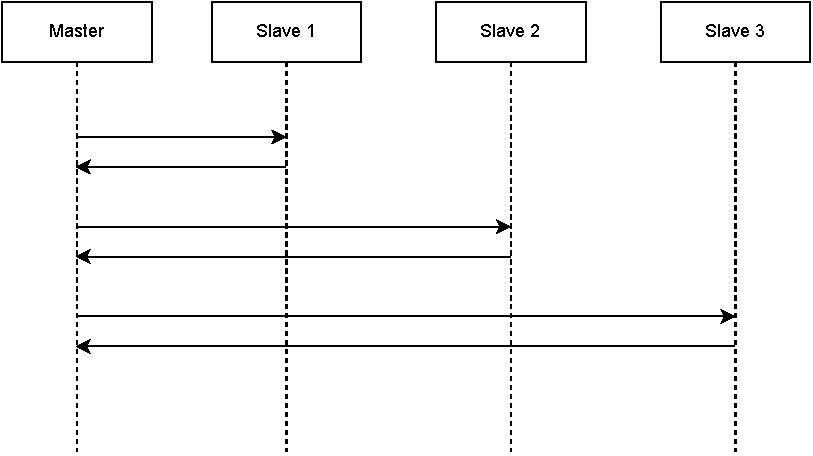
\includegraphics[width=0.7\textwidth]{obrazky-figures/master-oriented.pdf}
	\caption{Schéma komunikace \emph{master-oriented} profilu. Řídící stanice periodicky komunikuje s množinou podřízených stanic a obsluhuje vždy pouze jednu podřízenou stanici. Z~toho vyplývá, že komunikace probíhá v jednom okamžiku pouze mezi dvěma zařízeními \cite{anomaly_detection_ics}.}
	\label{master-oriented}
\end{figure}




\section{Datové sady s útoky}
\label{attack_datasets}

Datové sady s útoky vznikly v rámci projektu \emph{Bezpečnostní monitorování řídící komunikace ICS v energetických sítích (BONNET)}\footnote{\url{https://www.fit.vut.cz/research/project/1303/.en}} na \emph{Fakultě informačních technologií Vysokého učení technického v Brně}. Sady obsahují záznamy komunikace, ve které byl uměle nasimulován útok nebo anomálie. Jedná se o upravené verze jedné ze základních sad představených v~podkapitole \ref{basic_datasets}, konkrétně sady B. Všechny útoky byly generovány na aplikační vrstvě. Názvy sad a jejich popis je uveden výčtem:

\begin{itemize}
    \item \texttt{connection-loss.cvs:} v rámci komunikace dochází dvakrát ke ztrátě spojení. Konkrétně v časech:
    \begin{enumerate}
        \item od 16:27:57.68 do 16:37:48.63 (10 minut, 146 chybějících paketů)
        \item od 08:08:01.20 do 09:08:25.95 (1 hodina, 921 chybějících paketů)
    \end{enumerate}
    \item \texttt{switching-attack.csv:} cílem útoku je zapnutí/vypnutí zařízení. Celkově je odesláno 24 sérií paketů s parametry $asduType=46$ (Double cmd), $numix=1$, $cot=6$ (Act), $cot=7$ (ActCon), $cot=10$ (ActTerm), $oa=0$, $addr=655535$, $ioa=2$. Útok začíná v čase 06:27:55:00, trvá 10 minut a do komunikace zanáší 72 nových paketů.
    
    \item \texttt{scanning-attack.csv:}
    horizontální a vertikální skenování. Útok tohoto typu je možné provést díky zranitelnosti IEC 104 protokolu popsané v sekci \emph{Neautentizovaný přístup} v podkapitole \ref{unauthorized_access}.
    \begin{enumerate}
        \item 
        Cílem horizontálního skenování je nalezení IP adresy řídící stanice. Útok začíná v čase 10:32:07 a končí v 10:49:10.
        Z podvržené adresy \texttt{192.168.11.102:45280} jsou odesílány IEC 104 U-příkazy \emph{TestFrame Act} (s atributy $fmt=0x03$, $uType=0x10$) na port 2404 používaný řídící stanicí. Pokud se řídící stanice na dané IP adrese nachází, odpoví paketem \emph{TestFrame Conf} (s atributy $fmt=0x03$, $uType=0x20$).
    
        \item 
        \sloppy Vertikální skenování prozkoumává informační objekty zařízení. V tomto případě je útok směřován na zařízení s IP adresou \texttt{192.168.11.111}. Za účelem skrytí své identity, používá útočník podvrženou IP adresu \texttt{192.168.11.248}, která patří řídící stanici. Útočník odesílá dotaz s atributy $asduType=100$ (General Interrogation) a $cot=6$ (Activation). Pokud  informační objekt existuje, odesílá napadené zařízení odpověď s atributy $asduType=100$ (General Interrogation) a~$cot=7$ (Activation Conf), jinak odesílá odpoveď s atributem $cot=47$ (Unknown object address). K útoku se využívají výchozí hodnoty atributů $addr=65535$ a~$oa=0$. Přestože je ioa adresa dlouhá 16 bitů (a může tedy nabývat $2^{16}$ hodnot), útok prohledává pouze hodnoty adres od 0 do 127. Útok začíná v čase 01:02:18 a končí v 01:23:19.
    \end{enumerate}
    \item \texttt{dos-attack.csv:}
    útočník se snaží zahltit systém stovkami legitimních požadavků. K tomu používá podvrženou IP adresu \texttt{192.168.11.248}, ze které posílá pakety s~atributy $asduType=36$ (Measured value, short floating point, with time tag) a~$cot=3$ (Spontaneous event). Útok začíná v 23:50:02 a končí v 01:18:29. Obsahuje celkově 1049 podvržených požadavků. Další útok je opakován v 02:30:05 a trvá do 04:01:54.
    
    \item \texttt{rogue-devices.csv:}
    do systému je zaneseno tzv. \emph{rogue}\footnote{Zařízení, které je neoprávněně zavedeno do sítě, za účelem poškození provozovatele sítě. Může např. odposlouchávat komunikaci v síti, odesílat podvržené kontrolní příkazy jiným zařízením nebo provádět jiné aktivity, které představují bezpečnostní hrozbu pro provozovatele nebo uživatele sítě.} zařízení, které se vydává za legitimní IEC 104 zařízení s IP adresou \texttt{192.168.11.246}. Útočník používá ke komunikaci sekvenci paketů s atributy $asduType=36$ (Measured value, short floating point with time tag) a $cot=3$ (Spontaneous event). Útok začíná v 15:19:00 a končí v~15:46:03.
    
    \item \texttt{injection-attack.cvs:}
    Útočník odesílá neobvyklé požadavky s atributy $asduType=45$ (Single command) a $cot=6$ (Activation) na informační objekt s $ioa \subseteq \{2, 31, 32 \}$. Zacílená stanice odesílá odpověď s parametrem $cot=7$ (Activation Conf). Útok začíná v 19:35:19, končí v 19:41:06 a skládá se z 83 paketů.
    
    Další útok typu \emph{injection attack} se objevuje v 21:05:32, kdy útočník zahájí přenos souboru do napadené stanice s IP adresou \texttt{192.168.11.111}. Útočník odesílá pakety s atributy $asduType$ 122 (Call directory, select file), 120 (File ready), 121 (Section ready), 123 (Last section), 124 (Ack file) a 125 (Segment). Útočník přistupuje k informačnímu objektu s $ioa=65537$, který není typicky přístupný. Útok končí v 21:21:14 a skládá se z 221 paketů.
\end{itemize}



\section{Atributy datových sad}

Všechny popsané sady obsahují těchto 16 atributů:

\begin{itemize}
    \item \textbf{TimeStamp:} Časové razítko paketu.
    \item \textbf{Relative Time:} Relativní čas zachycení paketu v rámci datové sady v sekundách.
    \item \textbf{srcIP:} IP adresa zdrojové stanice.
    \item \textbf{dstIP:} IP adresa cílové stanice.
    \item \textbf{srcPort:} Port zdrojové stanice.
    \item \textbf{dstPort:} Port cílové stanice.
    \item \textbf{ipLen:} Délka IP paketu.
    \item \textbf{len:} Délka aplikačních dat.
    \item \textbf{fmt:} Formát APCI jednotky (viz \ref{apci_unit}). Konkrétní hodnoty vyskytující se v dostupných datových sadách:
    \begin{itemize}
        \item \texttt{0x00}: I-format
        \item \texttt{0x01}: S-format
        \item \texttt{0x03}: U-format
    \end{itemize}
    \item \textbf{uType:} Funkce rámce, pouze pro pakety v U-formátu.
    \item \textbf{asduType:} Typ ASDU jednotky. (viz \ref{asdu_types_table})
    \item \textbf{numix:} Počet hodnot v IOA poli.
    \item \textbf{cot:} Důvod přenosu (viz \ref{polozky_asdu}).
    \item \textbf{oa:} Adresa původce. Z angl. zkratky pro \emph{originator address}.
    \item \textbf{addr:} Linková adresa zařízení, může být dlouhá 8 nebo 16 bitů. Hodnoty \texttt{\#FF} a \texttt{\#FFFF} reprezentují broadcastové adresy.
    \item \textbf{ioa:} Pole adres informačních objektů (viz \ref{polozky_asdu}).
\end{itemize}


\label{polozky_datovych_sad}






\section{Metody popisu ICS komunikace}
\label{methods}

V této podkapitole budou představeny metody, které mohou být použity k analýze datových sad popsaných v podkapitolách \ref{basic_datasets} a \ref{attack_datasets}. Vhledy, které se analýzou získají, poskytují uživateli celkový přehled o odchycené komunikaci a~umožňují mu odhalit případné neočekávané události, útoky a anomálie.

\subsection{Počet paketů v čase}
\label{packet_counting}

Jendou z nejzákladnějších vlastností, kterou lze u průmyslové komunikace sledovat, je jednoduché měření počtu paketů v čase. Měření se většinou provádí pro jednu komunikační dvojici, ale lze provést agregovaně i pro více stanic současně. V první řadě je potřeba zvolit velikost časového okna, ve kterém se bude počet paketů měřit. Úskalí volby velikosti časového okna jsou popsány dále v této podkapitole v sekci \emph{Volba velikosti časového okna}. Výsledky lze vizualizovat pomocí spojnicového grafu. Graf přehledně zobrazuje počty paketů v jednotlivých časových oknech a jejich vývoj v čase. Uživatel by měl být schopen~z grafu vyčíst průběh sledované komunikace, její stabilitu, nebo případně nalézt její výpadky.

Jedním z možných rozšíření grafů, které vyobrazují komunikaci mezi dvěma stanicemi, je vynesení celkově tří křivek. Jednu křivku pro počet paketů ve směru od řídící stanici~k podřízené (dále jen \emph{M2S}), další pro počet paketů ve směru od podřízené stanice k řídící (dále jen \emph{S2M}) a poslední pro součet obou směrů. Ukázka rozšíření je znázorněna na obrázku \ref{graph1}.

\subsection*{Volba velikosti časového okna}
\label{time_window_size}

Volba velikosti časového okna je důležitým faktorem, který může představovat rozdíl mezi kvalitní a nekvalitní analýzou komunikace. Závisí na vlastnostech datové sady a na míře detailu, kterou uživatel vyžaduje. Ukázka dopadu velikosti časových oken na podobu spojnicových grafů je na obrázku \ref{fig:plot_var_sizes}.

V případě volby příliš malých časových oken, může dojít k vynulování některých oken a uživatel může nesprávně nabýt dojmu, že na některých místech došlo k výpadku komunikace. Ve skutečnosti je pouze velikost zvoleného časového okna menší než přirozená prodleva paketů v komunikaci. Příliš malé hodnoty také zanášejí do grafů šum, který ztěžuje jejich čitelnost (viz \ref{sub:first}).

V případě volby příliš velkých časových oken, můžou naopak některé výpadky být uživateli zcela skryty. Uživatel může např. zvolit 60 minutové okno a zkoumat komunikaci kde došlo k výpadku na 5 minut. V takovém případě bude vliv výpadku na hodnotu v časovém okně minimální a z grafu nebude možné anomálii vyčíst (viz \ref{sub:third}).


\begin{figure}[H]
	\centering
	\resizebox{1\textwidth}{!}
    {
        %% Creator: Matplotlib, PGF backend
%%
%% To include the figure in your LaTeX document, write
%%   \input{<filename>.pgf}
%%
%% Make sure the required packages are loaded in your preamble
%%   \usepackage{pgf}
%%
%% Also ensure that all the required font packages are loaded; for instance,
%% the lmodern package is sometimes necessary when using math font.
%%   \usepackage{lmodern}
%%
%% Figures using additional raster images can only be included by \input if
%% they are in the same directory as the main LaTeX file. For loading figures
%% from other directories you can use the `import` package
%%   \usepackage{import}
%%
%% and then include the figures with
%%   \import{<path to file>}{<filename>.pgf}
%%
%% Matplotlib used the following preamble
%%   \usepackage{fontspec}
%%   \setmainfont{DejaVuSerif.ttf}[Path=\detokenize{/home/ankimme/fit/ibt/env/lib/python3.10/site-packages/matplotlib/mpl-data/fonts/ttf/}]
%%   \setsansfont{DejaVuSans.ttf}[Path=\detokenize{/home/ankimme/fit/ibt/env/lib/python3.10/site-packages/matplotlib/mpl-data/fonts/ttf/}]
%%   \setmonofont{DejaVuSansMono.ttf}[Path=\detokenize{/home/ankimme/fit/ibt/env/lib/python3.10/site-packages/matplotlib/mpl-data/fonts/ttf/}]
%%
\begingroup%
\makeatletter%
\begin{pgfpicture}%
\pgfpathrectangle{\pgfpointorigin}{\pgfqpoint{10.000000in}{5.000000in}}%
\pgfusepath{use as bounding box, clip}%
\begin{pgfscope}%
\pgfsetbuttcap%
\pgfsetmiterjoin%
\pgfsetlinewidth{0.000000pt}%
\definecolor{currentstroke}{rgb}{1.000000,1.000000,1.000000}%
\pgfsetstrokecolor{currentstroke}%
\pgfsetstrokeopacity{0.000000}%
\pgfsetdash{}{0pt}%
\pgfpathmoveto{\pgfqpoint{0.000000in}{0.000000in}}%
\pgfpathlineto{\pgfqpoint{10.000000in}{0.000000in}}%
\pgfpathlineto{\pgfqpoint{10.000000in}{5.000000in}}%
\pgfpathlineto{\pgfqpoint{0.000000in}{5.000000in}}%
\pgfpathlineto{\pgfqpoint{0.000000in}{0.000000in}}%
\pgfpathclose%
\pgfusepath{}%
\end{pgfscope}%
\begin{pgfscope}%
\pgfsetbuttcap%
\pgfsetmiterjoin%
\definecolor{currentfill}{rgb}{1.000000,1.000000,1.000000}%
\pgfsetfillcolor{currentfill}%
\pgfsetlinewidth{0.000000pt}%
\definecolor{currentstroke}{rgb}{0.000000,0.000000,0.000000}%
\pgfsetstrokecolor{currentstroke}%
\pgfsetstrokeopacity{0.000000}%
\pgfsetdash{}{0pt}%
\pgfpathmoveto{\pgfqpoint{0.663435in}{0.517940in}}%
\pgfpathlineto{\pgfqpoint{9.958330in}{0.517940in}}%
\pgfpathlineto{\pgfqpoint{9.958330in}{4.561748in}}%
\pgfpathlineto{\pgfqpoint{0.663435in}{4.561748in}}%
\pgfpathlineto{\pgfqpoint{0.663435in}{0.517940in}}%
\pgfpathclose%
\pgfusepath{fill}%
\end{pgfscope}%
\begin{pgfscope}%
\pgfpathrectangle{\pgfqpoint{0.663435in}{0.517940in}}{\pgfqpoint{9.294895in}{4.043808in}}%
\pgfusepath{clip}%
\pgfsetrectcap%
\pgfsetroundjoin%
\pgfsetlinewidth{0.803000pt}%
\definecolor{currentstroke}{rgb}{0.690196,0.690196,0.690196}%
\pgfsetstrokecolor{currentstroke}%
\pgfsetdash{}{0pt}%
\pgfpathmoveto{\pgfqpoint{1.936776in}{0.517940in}}%
\pgfpathlineto{\pgfqpoint{1.936776in}{4.561748in}}%
\pgfusepath{stroke}%
\end{pgfscope}%
\begin{pgfscope}%
\pgfsetbuttcap%
\pgfsetroundjoin%
\definecolor{currentfill}{rgb}{0.000000,0.000000,0.000000}%
\pgfsetfillcolor{currentfill}%
\pgfsetlinewidth{0.803000pt}%
\definecolor{currentstroke}{rgb}{0.000000,0.000000,0.000000}%
\pgfsetstrokecolor{currentstroke}%
\pgfsetdash{}{0pt}%
\pgfsys@defobject{currentmarker}{\pgfqpoint{0.000000in}{-0.048611in}}{\pgfqpoint{0.000000in}{0.000000in}}{%
\pgfpathmoveto{\pgfqpoint{0.000000in}{0.000000in}}%
\pgfpathlineto{\pgfqpoint{0.000000in}{-0.048611in}}%
\pgfusepath{stroke,fill}%
}%
\begin{pgfscope}%
\pgfsys@transformshift{1.936776in}{0.517940in}%
\pgfsys@useobject{currentmarker}{}%
\end{pgfscope}%
\end{pgfscope}%
\begin{pgfscope}%
\definecolor{textcolor}{rgb}{0.000000,0.000000,0.000000}%
\pgfsetstrokecolor{textcolor}%
\pgfsetfillcolor{textcolor}%
\pgftext[x=1.936776in,y=0.420718in,,top]{\color{textcolor}\sffamily\fontsize{10.000000}{12.000000}\selectfont 00:00}%
\end{pgfscope}%
\begin{pgfscope}%
\pgfpathrectangle{\pgfqpoint{0.663435in}{0.517940in}}{\pgfqpoint{9.294895in}{4.043808in}}%
\pgfusepath{clip}%
\pgfsetrectcap%
\pgfsetroundjoin%
\pgfsetlinewidth{0.803000pt}%
\definecolor{currentstroke}{rgb}{0.690196,0.690196,0.690196}%
\pgfsetstrokecolor{currentstroke}%
\pgfsetdash{}{0pt}%
\pgfpathmoveto{\pgfqpoint{3.579060in}{0.517940in}}%
\pgfpathlineto{\pgfqpoint{3.579060in}{4.561748in}}%
\pgfusepath{stroke}%
\end{pgfscope}%
\begin{pgfscope}%
\pgfsetbuttcap%
\pgfsetroundjoin%
\definecolor{currentfill}{rgb}{0.000000,0.000000,0.000000}%
\pgfsetfillcolor{currentfill}%
\pgfsetlinewidth{0.803000pt}%
\definecolor{currentstroke}{rgb}{0.000000,0.000000,0.000000}%
\pgfsetstrokecolor{currentstroke}%
\pgfsetdash{}{0pt}%
\pgfsys@defobject{currentmarker}{\pgfqpoint{0.000000in}{-0.048611in}}{\pgfqpoint{0.000000in}{0.000000in}}{%
\pgfpathmoveto{\pgfqpoint{0.000000in}{0.000000in}}%
\pgfpathlineto{\pgfqpoint{0.000000in}{-0.048611in}}%
\pgfusepath{stroke,fill}%
}%
\begin{pgfscope}%
\pgfsys@transformshift{3.579060in}{0.517940in}%
\pgfsys@useobject{currentmarker}{}%
\end{pgfscope}%
\end{pgfscope}%
\begin{pgfscope}%
\definecolor{textcolor}{rgb}{0.000000,0.000000,0.000000}%
\pgfsetstrokecolor{textcolor}%
\pgfsetfillcolor{textcolor}%
\pgftext[x=3.579060in,y=0.420718in,,top]{\color{textcolor}\sffamily\fontsize{10.000000}{12.000000}\selectfont 12:00}%
\end{pgfscope}%
\begin{pgfscope}%
\pgfpathrectangle{\pgfqpoint{0.663435in}{0.517940in}}{\pgfqpoint{9.294895in}{4.043808in}}%
\pgfusepath{clip}%
\pgfsetrectcap%
\pgfsetroundjoin%
\pgfsetlinewidth{0.803000pt}%
\definecolor{currentstroke}{rgb}{0.690196,0.690196,0.690196}%
\pgfsetstrokecolor{currentstroke}%
\pgfsetdash{}{0pt}%
\pgfpathmoveto{\pgfqpoint{5.221345in}{0.517940in}}%
\pgfpathlineto{\pgfqpoint{5.221345in}{4.561748in}}%
\pgfusepath{stroke}%
\end{pgfscope}%
\begin{pgfscope}%
\pgfsetbuttcap%
\pgfsetroundjoin%
\definecolor{currentfill}{rgb}{0.000000,0.000000,0.000000}%
\pgfsetfillcolor{currentfill}%
\pgfsetlinewidth{0.803000pt}%
\definecolor{currentstroke}{rgb}{0.000000,0.000000,0.000000}%
\pgfsetstrokecolor{currentstroke}%
\pgfsetdash{}{0pt}%
\pgfsys@defobject{currentmarker}{\pgfqpoint{0.000000in}{-0.048611in}}{\pgfqpoint{0.000000in}{0.000000in}}{%
\pgfpathmoveto{\pgfqpoint{0.000000in}{0.000000in}}%
\pgfpathlineto{\pgfqpoint{0.000000in}{-0.048611in}}%
\pgfusepath{stroke,fill}%
}%
\begin{pgfscope}%
\pgfsys@transformshift{5.221345in}{0.517940in}%
\pgfsys@useobject{currentmarker}{}%
\end{pgfscope}%
\end{pgfscope}%
\begin{pgfscope}%
\definecolor{textcolor}{rgb}{0.000000,0.000000,0.000000}%
\pgfsetstrokecolor{textcolor}%
\pgfsetfillcolor{textcolor}%
\pgftext[x=5.221345in,y=0.420718in,,top]{\color{textcolor}\sffamily\fontsize{10.000000}{12.000000}\selectfont 00:00}%
\end{pgfscope}%
\begin{pgfscope}%
\pgfpathrectangle{\pgfqpoint{0.663435in}{0.517940in}}{\pgfqpoint{9.294895in}{4.043808in}}%
\pgfusepath{clip}%
\pgfsetrectcap%
\pgfsetroundjoin%
\pgfsetlinewidth{0.803000pt}%
\definecolor{currentstroke}{rgb}{0.690196,0.690196,0.690196}%
\pgfsetstrokecolor{currentstroke}%
\pgfsetdash{}{0pt}%
\pgfpathmoveto{\pgfqpoint{6.863629in}{0.517940in}}%
\pgfpathlineto{\pgfqpoint{6.863629in}{4.561748in}}%
\pgfusepath{stroke}%
\end{pgfscope}%
\begin{pgfscope}%
\pgfsetbuttcap%
\pgfsetroundjoin%
\definecolor{currentfill}{rgb}{0.000000,0.000000,0.000000}%
\pgfsetfillcolor{currentfill}%
\pgfsetlinewidth{0.803000pt}%
\definecolor{currentstroke}{rgb}{0.000000,0.000000,0.000000}%
\pgfsetstrokecolor{currentstroke}%
\pgfsetdash{}{0pt}%
\pgfsys@defobject{currentmarker}{\pgfqpoint{0.000000in}{-0.048611in}}{\pgfqpoint{0.000000in}{0.000000in}}{%
\pgfpathmoveto{\pgfqpoint{0.000000in}{0.000000in}}%
\pgfpathlineto{\pgfqpoint{0.000000in}{-0.048611in}}%
\pgfusepath{stroke,fill}%
}%
\begin{pgfscope}%
\pgfsys@transformshift{6.863629in}{0.517940in}%
\pgfsys@useobject{currentmarker}{}%
\end{pgfscope}%
\end{pgfscope}%
\begin{pgfscope}%
\definecolor{textcolor}{rgb}{0.000000,0.000000,0.000000}%
\pgfsetstrokecolor{textcolor}%
\pgfsetfillcolor{textcolor}%
\pgftext[x=6.863629in,y=0.420718in,,top]{\color{textcolor}\sffamily\fontsize{10.000000}{12.000000}\selectfont 12:00}%
\end{pgfscope}%
\begin{pgfscope}%
\pgfpathrectangle{\pgfqpoint{0.663435in}{0.517940in}}{\pgfqpoint{9.294895in}{4.043808in}}%
\pgfusepath{clip}%
\pgfsetrectcap%
\pgfsetroundjoin%
\pgfsetlinewidth{0.803000pt}%
\definecolor{currentstroke}{rgb}{0.690196,0.690196,0.690196}%
\pgfsetstrokecolor{currentstroke}%
\pgfsetdash{}{0pt}%
\pgfpathmoveto{\pgfqpoint{8.505913in}{0.517940in}}%
\pgfpathlineto{\pgfqpoint{8.505913in}{4.561748in}}%
\pgfusepath{stroke}%
\end{pgfscope}%
\begin{pgfscope}%
\pgfsetbuttcap%
\pgfsetroundjoin%
\definecolor{currentfill}{rgb}{0.000000,0.000000,0.000000}%
\pgfsetfillcolor{currentfill}%
\pgfsetlinewidth{0.803000pt}%
\definecolor{currentstroke}{rgb}{0.000000,0.000000,0.000000}%
\pgfsetstrokecolor{currentstroke}%
\pgfsetdash{}{0pt}%
\pgfsys@defobject{currentmarker}{\pgfqpoint{0.000000in}{-0.048611in}}{\pgfqpoint{0.000000in}{0.000000in}}{%
\pgfpathmoveto{\pgfqpoint{0.000000in}{0.000000in}}%
\pgfpathlineto{\pgfqpoint{0.000000in}{-0.048611in}}%
\pgfusepath{stroke,fill}%
}%
\begin{pgfscope}%
\pgfsys@transformshift{8.505913in}{0.517940in}%
\pgfsys@useobject{currentmarker}{}%
\end{pgfscope}%
\end{pgfscope}%
\begin{pgfscope}%
\definecolor{textcolor}{rgb}{0.000000,0.000000,0.000000}%
\pgfsetstrokecolor{textcolor}%
\pgfsetfillcolor{textcolor}%
\pgftext[x=8.505913in,y=0.420718in,,top]{\color{textcolor}\sffamily\fontsize{10.000000}{12.000000}\selectfont 00:00}%
\end{pgfscope}%
\begin{pgfscope}%
\definecolor{textcolor}{rgb}{0.000000,0.000000,0.000000}%
\pgfsetstrokecolor{textcolor}%
\pgfsetfillcolor{textcolor}%
\pgftext[x=5.310882in,y=0.230750in,,top]{\color{textcolor}\sffamily\fontsize{10.000000}{12.000000}\selectfont  }%
\end{pgfscope}%
\begin{pgfscope}%
\pgfpathrectangle{\pgfqpoint{0.663435in}{0.517940in}}{\pgfqpoint{9.294895in}{4.043808in}}%
\pgfusepath{clip}%
\pgfsetrectcap%
\pgfsetroundjoin%
\pgfsetlinewidth{0.803000pt}%
\definecolor{currentstroke}{rgb}{0.690196,0.690196,0.690196}%
\pgfsetstrokecolor{currentstroke}%
\pgfsetdash{}{0pt}%
\pgfpathmoveto{\pgfqpoint{0.663435in}{0.570457in}}%
\pgfpathlineto{\pgfqpoint{9.958330in}{0.570457in}}%
\pgfusepath{stroke}%
\end{pgfscope}%
\begin{pgfscope}%
\pgfsetbuttcap%
\pgfsetroundjoin%
\definecolor{currentfill}{rgb}{0.000000,0.000000,0.000000}%
\pgfsetfillcolor{currentfill}%
\pgfsetlinewidth{0.803000pt}%
\definecolor{currentstroke}{rgb}{0.000000,0.000000,0.000000}%
\pgfsetstrokecolor{currentstroke}%
\pgfsetdash{}{0pt}%
\pgfsys@defobject{currentmarker}{\pgfqpoint{-0.048611in}{0.000000in}}{\pgfqpoint{-0.000000in}{0.000000in}}{%
\pgfpathmoveto{\pgfqpoint{-0.000000in}{0.000000in}}%
\pgfpathlineto{\pgfqpoint{-0.048611in}{0.000000in}}%
\pgfusepath{stroke,fill}%
}%
\begin{pgfscope}%
\pgfsys@transformshift{0.663435in}{0.570457in}%
\pgfsys@useobject{currentmarker}{}%
\end{pgfscope}%
\end{pgfscope}%
\begin{pgfscope}%
\definecolor{textcolor}{rgb}{0.000000,0.000000,0.000000}%
\pgfsetstrokecolor{textcolor}%
\pgfsetfillcolor{textcolor}%
\pgftext[x=0.389482in, y=0.517696in, left, base]{\color{textcolor}\sffamily\fontsize{10.000000}{12.000000}\selectfont 25}%
\end{pgfscope}%
\begin{pgfscope}%
\pgfpathrectangle{\pgfqpoint{0.663435in}{0.517940in}}{\pgfqpoint{9.294895in}{4.043808in}}%
\pgfusepath{clip}%
\pgfsetrectcap%
\pgfsetroundjoin%
\pgfsetlinewidth{0.803000pt}%
\definecolor{currentstroke}{rgb}{0.690196,0.690196,0.690196}%
\pgfsetstrokecolor{currentstroke}%
\pgfsetdash{}{0pt}%
\pgfpathmoveto{\pgfqpoint{0.663435in}{1.117509in}}%
\pgfpathlineto{\pgfqpoint{9.958330in}{1.117509in}}%
\pgfusepath{stroke}%
\end{pgfscope}%
\begin{pgfscope}%
\pgfsetbuttcap%
\pgfsetroundjoin%
\definecolor{currentfill}{rgb}{0.000000,0.000000,0.000000}%
\pgfsetfillcolor{currentfill}%
\pgfsetlinewidth{0.803000pt}%
\definecolor{currentstroke}{rgb}{0.000000,0.000000,0.000000}%
\pgfsetstrokecolor{currentstroke}%
\pgfsetdash{}{0pt}%
\pgfsys@defobject{currentmarker}{\pgfqpoint{-0.048611in}{0.000000in}}{\pgfqpoint{-0.000000in}{0.000000in}}{%
\pgfpathmoveto{\pgfqpoint{-0.000000in}{0.000000in}}%
\pgfpathlineto{\pgfqpoint{-0.048611in}{0.000000in}}%
\pgfusepath{stroke,fill}%
}%
\begin{pgfscope}%
\pgfsys@transformshift{0.663435in}{1.117509in}%
\pgfsys@useobject{currentmarker}{}%
\end{pgfscope}%
\end{pgfscope}%
\begin{pgfscope}%
\definecolor{textcolor}{rgb}{0.000000,0.000000,0.000000}%
\pgfsetstrokecolor{textcolor}%
\pgfsetfillcolor{textcolor}%
\pgftext[x=0.389482in, y=1.064748in, left, base]{\color{textcolor}\sffamily\fontsize{10.000000}{12.000000}\selectfont 50}%
\end{pgfscope}%
\begin{pgfscope}%
\pgfpathrectangle{\pgfqpoint{0.663435in}{0.517940in}}{\pgfqpoint{9.294895in}{4.043808in}}%
\pgfusepath{clip}%
\pgfsetrectcap%
\pgfsetroundjoin%
\pgfsetlinewidth{0.803000pt}%
\definecolor{currentstroke}{rgb}{0.690196,0.690196,0.690196}%
\pgfsetstrokecolor{currentstroke}%
\pgfsetdash{}{0pt}%
\pgfpathmoveto{\pgfqpoint{0.663435in}{1.664561in}}%
\pgfpathlineto{\pgfqpoint{9.958330in}{1.664561in}}%
\pgfusepath{stroke}%
\end{pgfscope}%
\begin{pgfscope}%
\pgfsetbuttcap%
\pgfsetroundjoin%
\definecolor{currentfill}{rgb}{0.000000,0.000000,0.000000}%
\pgfsetfillcolor{currentfill}%
\pgfsetlinewidth{0.803000pt}%
\definecolor{currentstroke}{rgb}{0.000000,0.000000,0.000000}%
\pgfsetstrokecolor{currentstroke}%
\pgfsetdash{}{0pt}%
\pgfsys@defobject{currentmarker}{\pgfqpoint{-0.048611in}{0.000000in}}{\pgfqpoint{-0.000000in}{0.000000in}}{%
\pgfpathmoveto{\pgfqpoint{-0.000000in}{0.000000in}}%
\pgfpathlineto{\pgfqpoint{-0.048611in}{0.000000in}}%
\pgfusepath{stroke,fill}%
}%
\begin{pgfscope}%
\pgfsys@transformshift{0.663435in}{1.664561in}%
\pgfsys@useobject{currentmarker}{}%
\end{pgfscope}%
\end{pgfscope}%
\begin{pgfscope}%
\definecolor{textcolor}{rgb}{0.000000,0.000000,0.000000}%
\pgfsetstrokecolor{textcolor}%
\pgfsetfillcolor{textcolor}%
\pgftext[x=0.389482in, y=1.611800in, left, base]{\color{textcolor}\sffamily\fontsize{10.000000}{12.000000}\selectfont 75}%
\end{pgfscope}%
\begin{pgfscope}%
\pgfpathrectangle{\pgfqpoint{0.663435in}{0.517940in}}{\pgfqpoint{9.294895in}{4.043808in}}%
\pgfusepath{clip}%
\pgfsetrectcap%
\pgfsetroundjoin%
\pgfsetlinewidth{0.803000pt}%
\definecolor{currentstroke}{rgb}{0.690196,0.690196,0.690196}%
\pgfsetstrokecolor{currentstroke}%
\pgfsetdash{}{0pt}%
\pgfpathmoveto{\pgfqpoint{0.663435in}{2.211613in}}%
\pgfpathlineto{\pgfqpoint{9.958330in}{2.211613in}}%
\pgfusepath{stroke}%
\end{pgfscope}%
\begin{pgfscope}%
\pgfsetbuttcap%
\pgfsetroundjoin%
\definecolor{currentfill}{rgb}{0.000000,0.000000,0.000000}%
\pgfsetfillcolor{currentfill}%
\pgfsetlinewidth{0.803000pt}%
\definecolor{currentstroke}{rgb}{0.000000,0.000000,0.000000}%
\pgfsetstrokecolor{currentstroke}%
\pgfsetdash{}{0pt}%
\pgfsys@defobject{currentmarker}{\pgfqpoint{-0.048611in}{0.000000in}}{\pgfqpoint{-0.000000in}{0.000000in}}{%
\pgfpathmoveto{\pgfqpoint{-0.000000in}{0.000000in}}%
\pgfpathlineto{\pgfqpoint{-0.048611in}{0.000000in}}%
\pgfusepath{stroke,fill}%
}%
\begin{pgfscope}%
\pgfsys@transformshift{0.663435in}{2.211613in}%
\pgfsys@useobject{currentmarker}{}%
\end{pgfscope}%
\end{pgfscope}%
\begin{pgfscope}%
\definecolor{textcolor}{rgb}{0.000000,0.000000,0.000000}%
\pgfsetstrokecolor{textcolor}%
\pgfsetfillcolor{textcolor}%
\pgftext[x=0.301117in, y=2.158852in, left, base]{\color{textcolor}\sffamily\fontsize{10.000000}{12.000000}\selectfont 100}%
\end{pgfscope}%
\begin{pgfscope}%
\pgfpathrectangle{\pgfqpoint{0.663435in}{0.517940in}}{\pgfqpoint{9.294895in}{4.043808in}}%
\pgfusepath{clip}%
\pgfsetrectcap%
\pgfsetroundjoin%
\pgfsetlinewidth{0.803000pt}%
\definecolor{currentstroke}{rgb}{0.690196,0.690196,0.690196}%
\pgfsetstrokecolor{currentstroke}%
\pgfsetdash{}{0pt}%
\pgfpathmoveto{\pgfqpoint{0.663435in}{2.758665in}}%
\pgfpathlineto{\pgfqpoint{9.958330in}{2.758665in}}%
\pgfusepath{stroke}%
\end{pgfscope}%
\begin{pgfscope}%
\pgfsetbuttcap%
\pgfsetroundjoin%
\definecolor{currentfill}{rgb}{0.000000,0.000000,0.000000}%
\pgfsetfillcolor{currentfill}%
\pgfsetlinewidth{0.803000pt}%
\definecolor{currentstroke}{rgb}{0.000000,0.000000,0.000000}%
\pgfsetstrokecolor{currentstroke}%
\pgfsetdash{}{0pt}%
\pgfsys@defobject{currentmarker}{\pgfqpoint{-0.048611in}{0.000000in}}{\pgfqpoint{-0.000000in}{0.000000in}}{%
\pgfpathmoveto{\pgfqpoint{-0.000000in}{0.000000in}}%
\pgfpathlineto{\pgfqpoint{-0.048611in}{0.000000in}}%
\pgfusepath{stroke,fill}%
}%
\begin{pgfscope}%
\pgfsys@transformshift{0.663435in}{2.758665in}%
\pgfsys@useobject{currentmarker}{}%
\end{pgfscope}%
\end{pgfscope}%
\begin{pgfscope}%
\definecolor{textcolor}{rgb}{0.000000,0.000000,0.000000}%
\pgfsetstrokecolor{textcolor}%
\pgfsetfillcolor{textcolor}%
\pgftext[x=0.301117in, y=2.705903in, left, base]{\color{textcolor}\sffamily\fontsize{10.000000}{12.000000}\selectfont 125}%
\end{pgfscope}%
\begin{pgfscope}%
\pgfpathrectangle{\pgfqpoint{0.663435in}{0.517940in}}{\pgfqpoint{9.294895in}{4.043808in}}%
\pgfusepath{clip}%
\pgfsetrectcap%
\pgfsetroundjoin%
\pgfsetlinewidth{0.803000pt}%
\definecolor{currentstroke}{rgb}{0.690196,0.690196,0.690196}%
\pgfsetstrokecolor{currentstroke}%
\pgfsetdash{}{0pt}%
\pgfpathmoveto{\pgfqpoint{0.663435in}{3.305717in}}%
\pgfpathlineto{\pgfqpoint{9.958330in}{3.305717in}}%
\pgfusepath{stroke}%
\end{pgfscope}%
\begin{pgfscope}%
\pgfsetbuttcap%
\pgfsetroundjoin%
\definecolor{currentfill}{rgb}{0.000000,0.000000,0.000000}%
\pgfsetfillcolor{currentfill}%
\pgfsetlinewidth{0.803000pt}%
\definecolor{currentstroke}{rgb}{0.000000,0.000000,0.000000}%
\pgfsetstrokecolor{currentstroke}%
\pgfsetdash{}{0pt}%
\pgfsys@defobject{currentmarker}{\pgfqpoint{-0.048611in}{0.000000in}}{\pgfqpoint{-0.000000in}{0.000000in}}{%
\pgfpathmoveto{\pgfqpoint{-0.000000in}{0.000000in}}%
\pgfpathlineto{\pgfqpoint{-0.048611in}{0.000000in}}%
\pgfusepath{stroke,fill}%
}%
\begin{pgfscope}%
\pgfsys@transformshift{0.663435in}{3.305717in}%
\pgfsys@useobject{currentmarker}{}%
\end{pgfscope}%
\end{pgfscope}%
\begin{pgfscope}%
\definecolor{textcolor}{rgb}{0.000000,0.000000,0.000000}%
\pgfsetstrokecolor{textcolor}%
\pgfsetfillcolor{textcolor}%
\pgftext[x=0.301117in, y=3.252955in, left, base]{\color{textcolor}\sffamily\fontsize{10.000000}{12.000000}\selectfont 150}%
\end{pgfscope}%
\begin{pgfscope}%
\pgfpathrectangle{\pgfqpoint{0.663435in}{0.517940in}}{\pgfqpoint{9.294895in}{4.043808in}}%
\pgfusepath{clip}%
\pgfsetrectcap%
\pgfsetroundjoin%
\pgfsetlinewidth{0.803000pt}%
\definecolor{currentstroke}{rgb}{0.690196,0.690196,0.690196}%
\pgfsetstrokecolor{currentstroke}%
\pgfsetdash{}{0pt}%
\pgfpathmoveto{\pgfqpoint{0.663435in}{3.852769in}}%
\pgfpathlineto{\pgfqpoint{9.958330in}{3.852769in}}%
\pgfusepath{stroke}%
\end{pgfscope}%
\begin{pgfscope}%
\pgfsetbuttcap%
\pgfsetroundjoin%
\definecolor{currentfill}{rgb}{0.000000,0.000000,0.000000}%
\pgfsetfillcolor{currentfill}%
\pgfsetlinewidth{0.803000pt}%
\definecolor{currentstroke}{rgb}{0.000000,0.000000,0.000000}%
\pgfsetstrokecolor{currentstroke}%
\pgfsetdash{}{0pt}%
\pgfsys@defobject{currentmarker}{\pgfqpoint{-0.048611in}{0.000000in}}{\pgfqpoint{-0.000000in}{0.000000in}}{%
\pgfpathmoveto{\pgfqpoint{-0.000000in}{0.000000in}}%
\pgfpathlineto{\pgfqpoint{-0.048611in}{0.000000in}}%
\pgfusepath{stroke,fill}%
}%
\begin{pgfscope}%
\pgfsys@transformshift{0.663435in}{3.852769in}%
\pgfsys@useobject{currentmarker}{}%
\end{pgfscope}%
\end{pgfscope}%
\begin{pgfscope}%
\definecolor{textcolor}{rgb}{0.000000,0.000000,0.000000}%
\pgfsetstrokecolor{textcolor}%
\pgfsetfillcolor{textcolor}%
\pgftext[x=0.301117in, y=3.800007in, left, base]{\color{textcolor}\sffamily\fontsize{10.000000}{12.000000}\selectfont 175}%
\end{pgfscope}%
\begin{pgfscope}%
\pgfpathrectangle{\pgfqpoint{0.663435in}{0.517940in}}{\pgfqpoint{9.294895in}{4.043808in}}%
\pgfusepath{clip}%
\pgfsetrectcap%
\pgfsetroundjoin%
\pgfsetlinewidth{0.803000pt}%
\definecolor{currentstroke}{rgb}{0.690196,0.690196,0.690196}%
\pgfsetstrokecolor{currentstroke}%
\pgfsetdash{}{0pt}%
\pgfpathmoveto{\pgfqpoint{0.663435in}{4.399821in}}%
\pgfpathlineto{\pgfqpoint{9.958330in}{4.399821in}}%
\pgfusepath{stroke}%
\end{pgfscope}%
\begin{pgfscope}%
\pgfsetbuttcap%
\pgfsetroundjoin%
\definecolor{currentfill}{rgb}{0.000000,0.000000,0.000000}%
\pgfsetfillcolor{currentfill}%
\pgfsetlinewidth{0.803000pt}%
\definecolor{currentstroke}{rgb}{0.000000,0.000000,0.000000}%
\pgfsetstrokecolor{currentstroke}%
\pgfsetdash{}{0pt}%
\pgfsys@defobject{currentmarker}{\pgfqpoint{-0.048611in}{0.000000in}}{\pgfqpoint{-0.000000in}{0.000000in}}{%
\pgfpathmoveto{\pgfqpoint{-0.000000in}{0.000000in}}%
\pgfpathlineto{\pgfqpoint{-0.048611in}{0.000000in}}%
\pgfusepath{stroke,fill}%
}%
\begin{pgfscope}%
\pgfsys@transformshift{0.663435in}{4.399821in}%
\pgfsys@useobject{currentmarker}{}%
\end{pgfscope}%
\end{pgfscope}%
\begin{pgfscope}%
\definecolor{textcolor}{rgb}{0.000000,0.000000,0.000000}%
\pgfsetstrokecolor{textcolor}%
\pgfsetfillcolor{textcolor}%
\pgftext[x=0.301117in, y=4.347059in, left, base]{\color{textcolor}\sffamily\fontsize{10.000000}{12.000000}\selectfont 200}%
\end{pgfscope}%
\begin{pgfscope}%
\pgfpathrectangle{\pgfqpoint{0.663435in}{0.517940in}}{\pgfqpoint{9.294895in}{4.043808in}}%
\pgfusepath{clip}%
\pgfsetrectcap%
\pgfsetroundjoin%
\pgfsetlinewidth{3.011250pt}%
\definecolor{currentstroke}{rgb}{0.121569,0.466667,0.705882}%
\pgfsetstrokecolor{currentstroke}%
\pgfsetdash{}{0pt}%
\pgfpathmoveto{\pgfqpoint{0.659444in}{3.196307in}}%
\pgfpathlineto{\pgfqpoint{0.682253in}{3.852769in}}%
\pgfpathlineto{\pgfqpoint{0.705063in}{3.655830in}}%
\pgfpathlineto{\pgfqpoint{0.727872in}{3.743358in}}%
\pgfpathlineto{\pgfqpoint{0.750682in}{3.743358in}}%
\pgfpathlineto{\pgfqpoint{0.773491in}{3.612066in}}%
\pgfpathlineto{\pgfqpoint{0.796301in}{3.852769in}}%
\pgfpathlineto{\pgfqpoint{0.819110in}{3.655830in}}%
\pgfpathlineto{\pgfqpoint{0.841920in}{3.568302in}}%
\pgfpathlineto{\pgfqpoint{0.864729in}{4.137236in}}%
\pgfpathlineto{\pgfqpoint{0.887539in}{3.852769in}}%
\pgfpathlineto{\pgfqpoint{0.910348in}{4.137236in}}%
\pgfpathlineto{\pgfqpoint{0.933158in}{3.984061in}}%
\pgfpathlineto{\pgfqpoint{0.955968in}{3.502656in}}%
\pgfpathlineto{\pgfqpoint{0.978777in}{3.962179in}}%
\pgfpathlineto{\pgfqpoint{1.001587in}{3.568302in}}%
\pgfpathlineto{\pgfqpoint{1.024396in}{3.655830in}}%
\pgfpathlineto{\pgfqpoint{1.047206in}{4.377939in}}%
\pgfpathlineto{\pgfqpoint{1.070015in}{3.940297in}}%
\pgfpathlineto{\pgfqpoint{1.092825in}{3.852769in}}%
\pgfpathlineto{\pgfqpoint{1.115634in}{3.524538in}}%
\pgfpathlineto{\pgfqpoint{1.138444in}{3.743358in}}%
\pgfpathlineto{\pgfqpoint{1.161253in}{3.655830in}}%
\pgfpathlineto{\pgfqpoint{1.184063in}{3.830887in}}%
\pgfpathlineto{\pgfqpoint{1.206872in}{3.874651in}}%
\pgfpathlineto{\pgfqpoint{1.229682in}{3.633948in}}%
\pgfpathlineto{\pgfqpoint{1.252491in}{3.612066in}}%
\pgfpathlineto{\pgfqpoint{1.275301in}{3.655830in}}%
\pgfpathlineto{\pgfqpoint{1.298110in}{3.480774in}}%
\pgfpathlineto{\pgfqpoint{1.320920in}{3.415127in}}%
\pgfpathlineto{\pgfqpoint{1.343729in}{3.065014in}}%
\pgfpathlineto{\pgfqpoint{1.366539in}{3.086896in}}%
\pgfpathlineto{\pgfqpoint{1.389348in}{3.283835in}}%
\pgfpathlineto{\pgfqpoint{1.412158in}{3.218189in}}%
\pgfpathlineto{\pgfqpoint{1.434967in}{2.999368in}}%
\pgfpathlineto{\pgfqpoint{1.457777in}{3.349481in}}%
\pgfpathlineto{\pgfqpoint{1.480586in}{3.108778in}}%
\pgfpathlineto{\pgfqpoint{1.503396in}{3.043132in}}%
\pgfpathlineto{\pgfqpoint{1.526205in}{3.568302in}}%
\pgfpathlineto{\pgfqpoint{1.549015in}{3.196307in}}%
\pgfpathlineto{\pgfqpoint{1.571824in}{3.086896in}}%
\pgfpathlineto{\pgfqpoint{1.594634in}{3.108778in}}%
\pgfpathlineto{\pgfqpoint{1.617443in}{3.371363in}}%
\pgfpathlineto{\pgfqpoint{1.640253in}{3.043132in}}%
\pgfpathlineto{\pgfqpoint{1.663062in}{3.480774in}}%
\pgfpathlineto{\pgfqpoint{1.685872in}{3.174424in}}%
\pgfpathlineto{\pgfqpoint{1.708681in}{3.196307in}}%
\pgfpathlineto{\pgfqpoint{1.731491in}{2.846193in}}%
\pgfpathlineto{\pgfqpoint{1.754300in}{2.802429in}}%
\pgfpathlineto{\pgfqpoint{1.777110in}{2.911840in}}%
\pgfpathlineto{\pgfqpoint{1.799919in}{2.933722in}}%
\pgfpathlineto{\pgfqpoint{1.822729in}{2.780547in}}%
\pgfpathlineto{\pgfqpoint{1.845538in}{2.583608in}}%
\pgfpathlineto{\pgfqpoint{1.868348in}{2.649255in}}%
\pgfpathlineto{\pgfqpoint{1.891157in}{2.649255in}}%
\pgfpathlineto{\pgfqpoint{1.913967in}{2.539844in}}%
\pgfpathlineto{\pgfqpoint{1.936776in}{2.758665in}}%
\pgfpathlineto{\pgfqpoint{1.959586in}{2.758665in}}%
\pgfpathlineto{\pgfqpoint{1.982395in}{2.474198in}}%
\pgfpathlineto{\pgfqpoint{2.005205in}{2.583608in}}%
\pgfpathlineto{\pgfqpoint{2.028014in}{2.517962in}}%
\pgfpathlineto{\pgfqpoint{2.050824in}{2.955604in}}%
\pgfpathlineto{\pgfqpoint{2.073633in}{2.539844in}}%
\pgfpathlineto{\pgfqpoint{2.096443in}{2.430434in}}%
\pgfpathlineto{\pgfqpoint{2.119252in}{2.911840in}}%
\pgfpathlineto{\pgfqpoint{2.142062in}{2.802429in}}%
\pgfpathlineto{\pgfqpoint{2.164871in}{2.846193in}}%
\pgfpathlineto{\pgfqpoint{2.187681in}{2.999368in}}%
\pgfpathlineto{\pgfqpoint{2.210490in}{2.824311in}}%
\pgfpathlineto{\pgfqpoint{2.233300in}{2.583608in}}%
\pgfpathlineto{\pgfqpoint{2.256109in}{2.561726in}}%
\pgfpathlineto{\pgfqpoint{2.278919in}{2.517962in}}%
\pgfpathlineto{\pgfqpoint{2.301728in}{2.452316in}}%
\pgfpathlineto{\pgfqpoint{2.324538in}{2.474198in}}%
\pgfpathlineto{\pgfqpoint{2.347347in}{2.561726in}}%
\pgfpathlineto{\pgfqpoint{2.370157in}{2.474198in}}%
\pgfpathlineto{\pgfqpoint{2.392966in}{2.671137in}}%
\pgfpathlineto{\pgfqpoint{2.415776in}{2.452316in}}%
\pgfpathlineto{\pgfqpoint{2.461395in}{2.583608in}}%
\pgfpathlineto{\pgfqpoint{2.484204in}{2.517962in}}%
\pgfpathlineto{\pgfqpoint{2.507014in}{2.714901in}}%
\pgfpathlineto{\pgfqpoint{2.529823in}{2.430434in}}%
\pgfpathlineto{\pgfqpoint{2.552633in}{2.583608in}}%
\pgfpathlineto{\pgfqpoint{2.575442in}{2.408552in}}%
\pgfpathlineto{\pgfqpoint{2.598252in}{2.714901in}}%
\pgfpathlineto{\pgfqpoint{2.621061in}{2.496080in}}%
\pgfpathlineto{\pgfqpoint{2.643871in}{2.583608in}}%
\pgfpathlineto{\pgfqpoint{2.666680in}{2.824311in}}%
\pgfpathlineto{\pgfqpoint{2.689490in}{2.714901in}}%
\pgfpathlineto{\pgfqpoint{2.712299in}{3.086896in}}%
\pgfpathlineto{\pgfqpoint{2.735109in}{3.108778in}}%
\pgfpathlineto{\pgfqpoint{2.757918in}{2.955604in}}%
\pgfpathlineto{\pgfqpoint{2.780728in}{2.889957in}}%
\pgfpathlineto{\pgfqpoint{2.803537in}{2.868075in}}%
\pgfpathlineto{\pgfqpoint{2.826347in}{2.889957in}}%
\pgfpathlineto{\pgfqpoint{2.849156in}{3.174424in}}%
\pgfpathlineto{\pgfqpoint{2.871966in}{3.349481in}}%
\pgfpathlineto{\pgfqpoint{2.894775in}{3.108778in}}%
\pgfpathlineto{\pgfqpoint{2.917585in}{3.261953in}}%
\pgfpathlineto{\pgfqpoint{2.940394in}{3.152542in}}%
\pgfpathlineto{\pgfqpoint{2.963204in}{3.108778in}}%
\pgfpathlineto{\pgfqpoint{2.986013in}{3.043132in}}%
\pgfpathlineto{\pgfqpoint{3.008823in}{3.568302in}}%
\pgfpathlineto{\pgfqpoint{3.031632in}{3.261953in}}%
\pgfpathlineto{\pgfqpoint{3.054442in}{3.283835in}}%
\pgfpathlineto{\pgfqpoint{3.077251in}{2.933722in}}%
\pgfpathlineto{\pgfqpoint{3.100061in}{3.349481in}}%
\pgfpathlineto{\pgfqpoint{3.122870in}{3.458891in}}%
\pgfpathlineto{\pgfqpoint{3.145680in}{3.240071in}}%
\pgfpathlineto{\pgfqpoint{3.168489in}{3.480774in}}%
\pgfpathlineto{\pgfqpoint{3.191299in}{3.371363in}}%
\pgfpathlineto{\pgfqpoint{3.214108in}{3.349481in}}%
\pgfpathlineto{\pgfqpoint{3.236918in}{3.677712in}}%
\pgfpathlineto{\pgfqpoint{3.259727in}{3.086896in}}%
\pgfpathlineto{\pgfqpoint{3.282537in}{3.502656in}}%
\pgfpathlineto{\pgfqpoint{3.305346in}{3.327599in}}%
\pgfpathlineto{\pgfqpoint{3.328156in}{3.721476in}}%
\pgfpathlineto{\pgfqpoint{3.350965in}{3.699594in}}%
\pgfpathlineto{\pgfqpoint{3.373775in}{3.415127in}}%
\pgfpathlineto{\pgfqpoint{3.396584in}{3.240071in}}%
\pgfpathlineto{\pgfqpoint{3.419394in}{3.480774in}}%
\pgfpathlineto{\pgfqpoint{3.442203in}{3.458891in}}%
\pgfpathlineto{\pgfqpoint{3.465013in}{3.240071in}}%
\pgfpathlineto{\pgfqpoint{3.487822in}{3.546420in}}%
\pgfpathlineto{\pgfqpoint{3.510632in}{3.349481in}}%
\pgfpathlineto{\pgfqpoint{3.533441in}{3.502656in}}%
\pgfpathlineto{\pgfqpoint{3.556251in}{3.218189in}}%
\pgfpathlineto{\pgfqpoint{3.579060in}{3.502656in}}%
\pgfpathlineto{\pgfqpoint{3.601870in}{3.458891in}}%
\pgfpathlineto{\pgfqpoint{3.624679in}{3.480774in}}%
\pgfpathlineto{\pgfqpoint{3.647489in}{3.305717in}}%
\pgfpathlineto{\pgfqpoint{3.670298in}{3.480774in}}%
\pgfpathlineto{\pgfqpoint{3.693108in}{3.371363in}}%
\pgfpathlineto{\pgfqpoint{3.715917in}{3.524538in}}%
\pgfpathlineto{\pgfqpoint{3.738727in}{3.393245in}}%
\pgfpathlineto{\pgfqpoint{3.761536in}{3.349481in}}%
\pgfpathlineto{\pgfqpoint{3.784346in}{3.612066in}}%
\pgfpathlineto{\pgfqpoint{3.807155in}{3.633948in}}%
\pgfpathlineto{\pgfqpoint{3.829965in}{3.677712in}}%
\pgfpathlineto{\pgfqpoint{3.852774in}{3.240071in}}%
\pgfpathlineto{\pgfqpoint{3.875584in}{3.502656in}}%
\pgfpathlineto{\pgfqpoint{3.898393in}{3.568302in}}%
\pgfpathlineto{\pgfqpoint{3.921203in}{3.327599in}}%
\pgfpathlineto{\pgfqpoint{3.944012in}{3.152542in}}%
\pgfpathlineto{\pgfqpoint{3.966822in}{3.174424in}}%
\pgfpathlineto{\pgfqpoint{3.989631in}{3.568302in}}%
\pgfpathlineto{\pgfqpoint{4.012441in}{3.261953in}}%
\pgfpathlineto{\pgfqpoint{4.035250in}{3.458891in}}%
\pgfpathlineto{\pgfqpoint{4.058060in}{3.393245in}}%
\pgfpathlineto{\pgfqpoint{4.080869in}{3.371363in}}%
\pgfpathlineto{\pgfqpoint{4.103679in}{3.437009in}}%
\pgfpathlineto{\pgfqpoint{4.126489in}{3.371363in}}%
\pgfpathlineto{\pgfqpoint{4.149298in}{3.502656in}}%
\pgfpathlineto{\pgfqpoint{4.172108in}{3.283835in}}%
\pgfpathlineto{\pgfqpoint{4.194917in}{3.261953in}}%
\pgfpathlineto{\pgfqpoint{4.217727in}{3.415127in}}%
\pgfpathlineto{\pgfqpoint{4.240536in}{3.437009in}}%
\pgfpathlineto{\pgfqpoint{4.263346in}{3.437009in}}%
\pgfpathlineto{\pgfqpoint{4.286155in}{3.415127in}}%
\pgfpathlineto{\pgfqpoint{4.308965in}{3.174424in}}%
\pgfpathlineto{\pgfqpoint{4.331774in}{3.349481in}}%
\pgfpathlineto{\pgfqpoint{4.354584in}{3.546420in}}%
\pgfpathlineto{\pgfqpoint{4.377393in}{3.261953in}}%
\pgfpathlineto{\pgfqpoint{4.400203in}{3.108778in}}%
\pgfpathlineto{\pgfqpoint{4.423012in}{3.174424in}}%
\pgfpathlineto{\pgfqpoint{4.445822in}{3.174424in}}%
\pgfpathlineto{\pgfqpoint{4.468631in}{3.261953in}}%
\pgfpathlineto{\pgfqpoint{4.491441in}{3.327599in}}%
\pgfpathlineto{\pgfqpoint{4.514250in}{3.196307in}}%
\pgfpathlineto{\pgfqpoint{4.537060in}{3.415127in}}%
\pgfpathlineto{\pgfqpoint{4.559869in}{3.261953in}}%
\pgfpathlineto{\pgfqpoint{4.582679in}{3.415127in}}%
\pgfpathlineto{\pgfqpoint{4.605488in}{3.174424in}}%
\pgfpathlineto{\pgfqpoint{4.628298in}{3.305717in}}%
\pgfpathlineto{\pgfqpoint{4.651107in}{3.327599in}}%
\pgfpathlineto{\pgfqpoint{4.673917in}{3.218189in}}%
\pgfpathlineto{\pgfqpoint{4.696726in}{3.371363in}}%
\pgfpathlineto{\pgfqpoint{4.719536in}{3.502656in}}%
\pgfpathlineto{\pgfqpoint{4.742345in}{3.261953in}}%
\pgfpathlineto{\pgfqpoint{4.765155in}{3.283835in}}%
\pgfpathlineto{\pgfqpoint{4.787964in}{3.261953in}}%
\pgfpathlineto{\pgfqpoint{4.810774in}{2.955604in}}%
\pgfpathlineto{\pgfqpoint{4.833583in}{3.196307in}}%
\pgfpathlineto{\pgfqpoint{4.856393in}{3.240071in}}%
\pgfpathlineto{\pgfqpoint{4.879202in}{3.371363in}}%
\pgfpathlineto{\pgfqpoint{4.902012in}{3.393245in}}%
\pgfpathlineto{\pgfqpoint{4.924821in}{3.196307in}}%
\pgfpathlineto{\pgfqpoint{4.947631in}{3.065014in}}%
\pgfpathlineto{\pgfqpoint{4.970440in}{3.174424in}}%
\pgfpathlineto{\pgfqpoint{4.993250in}{3.043132in}}%
\pgfpathlineto{\pgfqpoint{5.016059in}{2.868075in}}%
\pgfpathlineto{\pgfqpoint{5.038869in}{3.086896in}}%
\pgfpathlineto{\pgfqpoint{5.061678in}{3.086896in}}%
\pgfpathlineto{\pgfqpoint{5.084488in}{2.977486in}}%
\pgfpathlineto{\pgfqpoint{5.107297in}{2.977486in}}%
\pgfpathlineto{\pgfqpoint{5.130107in}{2.627373in}}%
\pgfpathlineto{\pgfqpoint{5.152916in}{2.474198in}}%
\pgfpathlineto{\pgfqpoint{5.175726in}{2.693019in}}%
\pgfpathlineto{\pgfqpoint{5.198535in}{2.736783in}}%
\pgfpathlineto{\pgfqpoint{5.221345in}{2.539844in}}%
\pgfpathlineto{\pgfqpoint{5.244154in}{2.561726in}}%
\pgfpathlineto{\pgfqpoint{5.266964in}{2.496080in}}%
\pgfpathlineto{\pgfqpoint{5.289773in}{2.583608in}}%
\pgfpathlineto{\pgfqpoint{5.312583in}{2.583608in}}%
\pgfpathlineto{\pgfqpoint{5.335392in}{2.539844in}}%
\pgfpathlineto{\pgfqpoint{5.358202in}{2.780547in}}%
\pgfpathlineto{\pgfqpoint{5.381011in}{2.539844in}}%
\pgfpathlineto{\pgfqpoint{5.403821in}{2.780547in}}%
\pgfpathlineto{\pgfqpoint{5.426630in}{2.539844in}}%
\pgfpathlineto{\pgfqpoint{5.449440in}{2.671137in}}%
\pgfpathlineto{\pgfqpoint{5.472249in}{2.671137in}}%
\pgfpathlineto{\pgfqpoint{5.495059in}{2.496080in}}%
\pgfpathlineto{\pgfqpoint{5.517868in}{2.474198in}}%
\pgfpathlineto{\pgfqpoint{5.540678in}{2.583608in}}%
\pgfpathlineto{\pgfqpoint{5.563487in}{2.539844in}}%
\pgfpathlineto{\pgfqpoint{5.586297in}{2.846193in}}%
\pgfpathlineto{\pgfqpoint{5.609106in}{2.605490in}}%
\pgfpathlineto{\pgfqpoint{5.631916in}{2.496080in}}%
\pgfpathlineto{\pgfqpoint{5.654725in}{2.430434in}}%
\pgfpathlineto{\pgfqpoint{5.677535in}{2.561726in}}%
\pgfpathlineto{\pgfqpoint{5.700344in}{2.605490in}}%
\pgfpathlineto{\pgfqpoint{5.723154in}{2.583608in}}%
\pgfpathlineto{\pgfqpoint{5.745963in}{2.605490in}}%
\pgfpathlineto{\pgfqpoint{5.768773in}{2.474198in}}%
\pgfpathlineto{\pgfqpoint{5.791582in}{2.605490in}}%
\pgfpathlineto{\pgfqpoint{5.814392in}{2.605490in}}%
\pgfpathlineto{\pgfqpoint{5.837201in}{2.452316in}}%
\pgfpathlineto{\pgfqpoint{5.860011in}{2.780547in}}%
\pgfpathlineto{\pgfqpoint{5.882820in}{2.758665in}}%
\pgfpathlineto{\pgfqpoint{5.905630in}{2.889957in}}%
\pgfpathlineto{\pgfqpoint{5.928439in}{2.758665in}}%
\pgfpathlineto{\pgfqpoint{5.951249in}{2.736783in}}%
\pgfpathlineto{\pgfqpoint{5.974058in}{3.043132in}}%
\pgfpathlineto{\pgfqpoint{5.996868in}{2.933722in}}%
\pgfpathlineto{\pgfqpoint{6.019677in}{2.868075in}}%
\pgfpathlineto{\pgfqpoint{6.042487in}{2.758665in}}%
\pgfpathlineto{\pgfqpoint{6.065296in}{3.086896in}}%
\pgfpathlineto{\pgfqpoint{6.088106in}{2.868075in}}%
\pgfpathlineto{\pgfqpoint{6.110915in}{3.196307in}}%
\pgfpathlineto{\pgfqpoint{6.133725in}{3.349481in}}%
\pgfpathlineto{\pgfqpoint{6.156534in}{3.261953in}}%
\pgfpathlineto{\pgfqpoint{6.179344in}{2.889957in}}%
\pgfpathlineto{\pgfqpoint{6.202153in}{3.327599in}}%
\pgfpathlineto{\pgfqpoint{6.224963in}{2.999368in}}%
\pgfpathlineto{\pgfqpoint{6.247772in}{3.108778in}}%
\pgfpathlineto{\pgfqpoint{6.270582in}{3.305717in}}%
\pgfpathlineto{\pgfqpoint{6.293391in}{3.283835in}}%
\pgfpathlineto{\pgfqpoint{6.316201in}{3.305717in}}%
\pgfpathlineto{\pgfqpoint{6.339010in}{3.283835in}}%
\pgfpathlineto{\pgfqpoint{6.361820in}{3.437009in}}%
\pgfpathlineto{\pgfqpoint{6.384629in}{3.458891in}}%
\pgfpathlineto{\pgfqpoint{6.407439in}{3.458891in}}%
\pgfpathlineto{\pgfqpoint{6.453058in}{3.152542in}}%
\pgfpathlineto{\pgfqpoint{6.475867in}{3.371363in}}%
\pgfpathlineto{\pgfqpoint{6.498677in}{3.283835in}}%
\pgfpathlineto{\pgfqpoint{6.521486in}{3.437009in}}%
\pgfpathlineto{\pgfqpoint{6.544296in}{3.108778in}}%
\pgfpathlineto{\pgfqpoint{6.567105in}{3.743358in}}%
\pgfpathlineto{\pgfqpoint{6.589915in}{3.655830in}}%
\pgfpathlineto{\pgfqpoint{6.612724in}{3.174424in}}%
\pgfpathlineto{\pgfqpoint{6.635534in}{3.415127in}}%
\pgfpathlineto{\pgfqpoint{6.658343in}{3.415127in}}%
\pgfpathlineto{\pgfqpoint{6.681153in}{3.590184in}}%
\pgfpathlineto{\pgfqpoint{6.703962in}{3.524538in}}%
\pgfpathlineto{\pgfqpoint{6.726772in}{3.830887in}}%
\pgfpathlineto{\pgfqpoint{6.749581in}{3.655830in}}%
\pgfpathlineto{\pgfqpoint{6.772391in}{3.590184in}}%
\pgfpathlineto{\pgfqpoint{6.795200in}{3.699594in}}%
\pgfpathlineto{\pgfqpoint{6.818010in}{3.261953in}}%
\pgfpathlineto{\pgfqpoint{6.840819in}{3.437009in}}%
\pgfpathlineto{\pgfqpoint{6.863629in}{3.721476in}}%
\pgfpathlineto{\pgfqpoint{6.886438in}{3.458891in}}%
\pgfpathlineto{\pgfqpoint{6.909248in}{3.612066in}}%
\pgfpathlineto{\pgfqpoint{6.932057in}{3.305717in}}%
\pgfpathlineto{\pgfqpoint{6.954867in}{3.655830in}}%
\pgfpathlineto{\pgfqpoint{6.977676in}{3.261953in}}%
\pgfpathlineto{\pgfqpoint{7.000486in}{3.371363in}}%
\pgfpathlineto{\pgfqpoint{7.023295in}{3.415127in}}%
\pgfpathlineto{\pgfqpoint{7.046105in}{3.327599in}}%
\pgfpathlineto{\pgfqpoint{7.068914in}{3.349481in}}%
\pgfpathlineto{\pgfqpoint{7.091724in}{3.305717in}}%
\pgfpathlineto{\pgfqpoint{7.114533in}{3.349481in}}%
\pgfpathlineto{\pgfqpoint{7.137343in}{3.480774in}}%
\pgfpathlineto{\pgfqpoint{7.160152in}{3.218189in}}%
\pgfpathlineto{\pgfqpoint{7.182962in}{3.393245in}}%
\pgfpathlineto{\pgfqpoint{7.205771in}{3.415127in}}%
\pgfpathlineto{\pgfqpoint{7.228581in}{3.524538in}}%
\pgfpathlineto{\pgfqpoint{7.251390in}{3.415127in}}%
\pgfpathlineto{\pgfqpoint{7.274200in}{3.458891in}}%
\pgfpathlineto{\pgfqpoint{7.297010in}{3.218189in}}%
\pgfpathlineto{\pgfqpoint{7.319819in}{3.480774in}}%
\pgfpathlineto{\pgfqpoint{7.342629in}{3.524538in}}%
\pgfpathlineto{\pgfqpoint{7.365438in}{3.240071in}}%
\pgfpathlineto{\pgfqpoint{7.388248in}{3.371363in}}%
\pgfpathlineto{\pgfqpoint{7.411057in}{3.458891in}}%
\pgfpathlineto{\pgfqpoint{7.433867in}{3.152542in}}%
\pgfpathlineto{\pgfqpoint{7.456676in}{3.524538in}}%
\pgfpathlineto{\pgfqpoint{7.502295in}{3.218189in}}%
\pgfpathlineto{\pgfqpoint{7.525105in}{3.765241in}}%
\pgfpathlineto{\pgfqpoint{7.547914in}{3.677712in}}%
\pgfpathlineto{\pgfqpoint{7.570724in}{3.655830in}}%
\pgfpathlineto{\pgfqpoint{7.593533in}{3.415127in}}%
\pgfpathlineto{\pgfqpoint{7.616343in}{3.305717in}}%
\pgfpathlineto{\pgfqpoint{7.639152in}{3.765241in}}%
\pgfpathlineto{\pgfqpoint{7.661962in}{3.480774in}}%
\pgfpathlineto{\pgfqpoint{7.684771in}{3.393245in}}%
\pgfpathlineto{\pgfqpoint{7.707581in}{3.590184in}}%
\pgfpathlineto{\pgfqpoint{7.730390in}{3.152542in}}%
\pgfpathlineto{\pgfqpoint{7.753200in}{3.415127in}}%
\pgfpathlineto{\pgfqpoint{7.776009in}{3.502656in}}%
\pgfpathlineto{\pgfqpoint{7.798819in}{3.480774in}}%
\pgfpathlineto{\pgfqpoint{7.821628in}{3.480774in}}%
\pgfpathlineto{\pgfqpoint{7.844438in}{3.437009in}}%
\pgfpathlineto{\pgfqpoint{7.867247in}{3.283835in}}%
\pgfpathlineto{\pgfqpoint{7.890057in}{3.787123in}}%
\pgfpathlineto{\pgfqpoint{7.912866in}{3.305717in}}%
\pgfpathlineto{\pgfqpoint{7.935676in}{3.196307in}}%
\pgfpathlineto{\pgfqpoint{7.958485in}{3.261953in}}%
\pgfpathlineto{\pgfqpoint{7.981295in}{3.086896in}}%
\pgfpathlineto{\pgfqpoint{8.004104in}{3.327599in}}%
\pgfpathlineto{\pgfqpoint{8.026914in}{3.633948in}}%
\pgfpathlineto{\pgfqpoint{8.049723in}{3.283835in}}%
\pgfpathlineto{\pgfqpoint{8.072533in}{3.371363in}}%
\pgfpathlineto{\pgfqpoint{8.095342in}{3.305717in}}%
\pgfpathlineto{\pgfqpoint{8.118152in}{3.174424in}}%
\pgfpathlineto{\pgfqpoint{8.140961in}{3.218189in}}%
\pgfpathlineto{\pgfqpoint{8.163771in}{3.086896in}}%
\pgfpathlineto{\pgfqpoint{8.186580in}{2.933722in}}%
\pgfpathlineto{\pgfqpoint{8.209390in}{3.130660in}}%
\pgfpathlineto{\pgfqpoint{8.232199in}{3.108778in}}%
\pgfpathlineto{\pgfqpoint{8.255009in}{3.240071in}}%
\pgfpathlineto{\pgfqpoint{8.277818in}{3.152542in}}%
\pgfpathlineto{\pgfqpoint{8.300628in}{3.152542in}}%
\pgfpathlineto{\pgfqpoint{8.323437in}{3.086896in}}%
\pgfpathlineto{\pgfqpoint{8.346247in}{3.043132in}}%
\pgfpathlineto{\pgfqpoint{8.369056in}{2.955604in}}%
\pgfpathlineto{\pgfqpoint{8.391866in}{2.824311in}}%
\pgfpathlineto{\pgfqpoint{8.414675in}{2.780547in}}%
\pgfpathlineto{\pgfqpoint{8.437485in}{2.539844in}}%
\pgfpathlineto{\pgfqpoint{8.460294in}{2.649255in}}%
\pgfpathlineto{\pgfqpoint{8.483104in}{3.021250in}}%
\pgfpathlineto{\pgfqpoint{8.505913in}{2.605490in}}%
\pgfpathlineto{\pgfqpoint{8.528723in}{2.736783in}}%
\pgfpathlineto{\pgfqpoint{8.551532in}{2.408552in}}%
\pgfpathlineto{\pgfqpoint{8.574342in}{2.802429in}}%
\pgfpathlineto{\pgfqpoint{8.597151in}{2.649255in}}%
\pgfpathlineto{\pgfqpoint{8.619961in}{2.736783in}}%
\pgfpathlineto{\pgfqpoint{8.642770in}{2.605490in}}%
\pgfpathlineto{\pgfqpoint{8.665580in}{2.649255in}}%
\pgfpathlineto{\pgfqpoint{8.688389in}{2.583608in}}%
\pgfpathlineto{\pgfqpoint{8.711199in}{2.605490in}}%
\pgfpathlineto{\pgfqpoint{8.734008in}{2.255377in}}%
\pgfpathlineto{\pgfqpoint{8.756818in}{2.714901in}}%
\pgfpathlineto{\pgfqpoint{8.779627in}{2.452316in}}%
\pgfpathlineto{\pgfqpoint{8.802437in}{2.649255in}}%
\pgfpathlineto{\pgfqpoint{8.825246in}{2.321023in}}%
\pgfpathlineto{\pgfqpoint{8.848056in}{2.539844in}}%
\pgfpathlineto{\pgfqpoint{8.870865in}{2.583608in}}%
\pgfpathlineto{\pgfqpoint{8.893675in}{2.605490in}}%
\pgfpathlineto{\pgfqpoint{8.916484in}{2.649255in}}%
\pgfpathlineto{\pgfqpoint{8.939294in}{2.496080in}}%
\pgfpathlineto{\pgfqpoint{8.962103in}{2.583608in}}%
\pgfpathlineto{\pgfqpoint{8.984913in}{2.496080in}}%
\pgfpathlineto{\pgfqpoint{9.007722in}{2.430434in}}%
\pgfpathlineto{\pgfqpoint{9.030532in}{2.539844in}}%
\pgfpathlineto{\pgfqpoint{9.053341in}{2.561726in}}%
\pgfpathlineto{\pgfqpoint{9.076151in}{2.605490in}}%
\pgfpathlineto{\pgfqpoint{9.098960in}{2.539844in}}%
\pgfpathlineto{\pgfqpoint{9.121770in}{3.261953in}}%
\pgfpathlineto{\pgfqpoint{9.144579in}{3.043132in}}%
\pgfpathlineto{\pgfqpoint{9.167389in}{3.065014in}}%
\pgfpathlineto{\pgfqpoint{9.190198in}{3.327599in}}%
\pgfpathlineto{\pgfqpoint{9.213008in}{3.130660in}}%
\pgfpathlineto{\pgfqpoint{9.235817in}{3.261953in}}%
\pgfpathlineto{\pgfqpoint{9.258627in}{3.349481in}}%
\pgfpathlineto{\pgfqpoint{9.281436in}{3.502656in}}%
\pgfpathlineto{\pgfqpoint{9.304246in}{3.590184in}}%
\pgfpathlineto{\pgfqpoint{9.327055in}{3.502656in}}%
\pgfpathlineto{\pgfqpoint{9.349865in}{3.809005in}}%
\pgfpathlineto{\pgfqpoint{9.372674in}{3.393245in}}%
\pgfpathlineto{\pgfqpoint{9.395484in}{3.677712in}}%
\pgfpathlineto{\pgfqpoint{9.418293in}{3.524538in}}%
\pgfpathlineto{\pgfqpoint{9.441103in}{3.721476in}}%
\pgfpathlineto{\pgfqpoint{9.486722in}{4.071590in}}%
\pgfpathlineto{\pgfqpoint{9.509531in}{3.896533in}}%
\pgfpathlineto{\pgfqpoint{9.532341in}{3.918415in}}%
\pgfpathlineto{\pgfqpoint{9.555150in}{4.071590in}}%
\pgfpathlineto{\pgfqpoint{9.577960in}{3.918415in}}%
\pgfpathlineto{\pgfqpoint{9.600769in}{4.093472in}}%
\pgfpathlineto{\pgfqpoint{9.623579in}{3.568302in}}%
\pgfpathlineto{\pgfqpoint{9.646388in}{3.918415in}}%
\pgfpathlineto{\pgfqpoint{9.669198in}{4.049708in}}%
\pgfpathlineto{\pgfqpoint{9.692007in}{3.502656in}}%
\pgfpathlineto{\pgfqpoint{9.714817in}{3.699594in}}%
\pgfpathlineto{\pgfqpoint{9.737626in}{4.115354in}}%
\pgfpathlineto{\pgfqpoint{9.760436in}{3.437009in}}%
\pgfpathlineto{\pgfqpoint{9.783245in}{3.809005in}}%
\pgfpathlineto{\pgfqpoint{9.806055in}{3.699594in}}%
\pgfpathlineto{\pgfqpoint{9.828864in}{3.677712in}}%
\pgfpathlineto{\pgfqpoint{9.851674in}{3.699594in}}%
\pgfpathlineto{\pgfqpoint{9.874483in}{3.874651in}}%
\pgfpathlineto{\pgfqpoint{9.897293in}{3.787123in}}%
\pgfpathlineto{\pgfqpoint{9.920102in}{3.896533in}}%
\pgfpathlineto{\pgfqpoint{9.942912in}{2.496080in}}%
\pgfpathlineto{\pgfqpoint{9.942912in}{2.496080in}}%
\pgfusepath{stroke}%
\end{pgfscope}%
\begin{pgfscope}%
\pgfpathrectangle{\pgfqpoint{0.663435in}{0.517940in}}{\pgfqpoint{9.294895in}{4.043808in}}%
\pgfusepath{clip}%
\pgfsetrectcap%
\pgfsetroundjoin%
\pgfsetlinewidth{3.011250pt}%
\definecolor{currentstroke}{rgb}{1.000000,0.498039,0.054902}%
\pgfsetstrokecolor{currentstroke}%
\pgfsetdash{}{0pt}%
\pgfpathmoveto{\pgfqpoint{0.659444in}{0.876806in}}%
\pgfpathlineto{\pgfqpoint{0.682253in}{1.117509in}}%
\pgfpathlineto{\pgfqpoint{0.727872in}{1.029981in}}%
\pgfpathlineto{\pgfqpoint{0.750682in}{1.029981in}}%
\pgfpathlineto{\pgfqpoint{0.773491in}{1.073745in}}%
\pgfpathlineto{\pgfqpoint{0.796301in}{1.051863in}}%
\pgfpathlineto{\pgfqpoint{0.819110in}{0.986217in}}%
\pgfpathlineto{\pgfqpoint{0.841920in}{1.029981in}}%
\pgfpathlineto{\pgfqpoint{0.887539in}{1.029981in}}%
\pgfpathlineto{\pgfqpoint{0.910348in}{1.073745in}}%
\pgfpathlineto{\pgfqpoint{0.933158in}{1.029981in}}%
\pgfpathlineto{\pgfqpoint{0.978777in}{1.073745in}}%
\pgfpathlineto{\pgfqpoint{1.001587in}{1.029981in}}%
\pgfpathlineto{\pgfqpoint{1.024396in}{1.029981in}}%
\pgfpathlineto{\pgfqpoint{1.047206in}{1.117509in}}%
\pgfpathlineto{\pgfqpoint{1.070015in}{1.051863in}}%
\pgfpathlineto{\pgfqpoint{1.115634in}{1.008099in}}%
\pgfpathlineto{\pgfqpoint{1.138444in}{1.008099in}}%
\pgfpathlineto{\pgfqpoint{1.161253in}{1.051863in}}%
\pgfpathlineto{\pgfqpoint{1.206872in}{1.051863in}}%
\pgfpathlineto{\pgfqpoint{1.229682in}{1.029981in}}%
\pgfpathlineto{\pgfqpoint{1.252491in}{1.029981in}}%
\pgfpathlineto{\pgfqpoint{1.275301in}{1.008099in}}%
\pgfpathlineto{\pgfqpoint{1.298110in}{1.051863in}}%
\pgfpathlineto{\pgfqpoint{1.320920in}{1.051863in}}%
\pgfpathlineto{\pgfqpoint{1.343729in}{0.964335in}}%
\pgfpathlineto{\pgfqpoint{1.366539in}{1.051863in}}%
\pgfpathlineto{\pgfqpoint{1.389348in}{1.029981in}}%
\pgfpathlineto{\pgfqpoint{1.412158in}{1.051863in}}%
\pgfpathlineto{\pgfqpoint{1.434967in}{0.986217in}}%
\pgfpathlineto{\pgfqpoint{1.457777in}{1.029981in}}%
\pgfpathlineto{\pgfqpoint{1.480586in}{1.008099in}}%
\pgfpathlineto{\pgfqpoint{1.526205in}{1.051863in}}%
\pgfpathlineto{\pgfqpoint{1.549015in}{1.095627in}}%
\pgfpathlineto{\pgfqpoint{1.571824in}{0.986217in}}%
\pgfpathlineto{\pgfqpoint{1.594634in}{0.964335in}}%
\pgfpathlineto{\pgfqpoint{1.617443in}{1.051863in}}%
\pgfpathlineto{\pgfqpoint{1.640253in}{0.986217in}}%
\pgfpathlineto{\pgfqpoint{1.663062in}{1.051863in}}%
\pgfpathlineto{\pgfqpoint{1.708681in}{1.008099in}}%
\pgfpathlineto{\pgfqpoint{1.822729in}{1.008099in}}%
\pgfpathlineto{\pgfqpoint{1.845538in}{0.964335in}}%
\pgfpathlineto{\pgfqpoint{1.868348in}{0.964335in}}%
\pgfpathlineto{\pgfqpoint{1.891157in}{1.029981in}}%
\pgfpathlineto{\pgfqpoint{1.913967in}{1.008099in}}%
\pgfpathlineto{\pgfqpoint{1.936776in}{1.008099in}}%
\pgfpathlineto{\pgfqpoint{1.959586in}{1.029981in}}%
\pgfpathlineto{\pgfqpoint{1.982395in}{0.964335in}}%
\pgfpathlineto{\pgfqpoint{2.005205in}{0.986217in}}%
\pgfpathlineto{\pgfqpoint{2.028014in}{0.964335in}}%
\pgfpathlineto{\pgfqpoint{2.096443in}{1.029981in}}%
\pgfpathlineto{\pgfqpoint{2.119252in}{0.942453in}}%
\pgfpathlineto{\pgfqpoint{2.142062in}{1.029981in}}%
\pgfpathlineto{\pgfqpoint{2.164871in}{1.008099in}}%
\pgfpathlineto{\pgfqpoint{2.210490in}{1.051863in}}%
\pgfpathlineto{\pgfqpoint{2.233300in}{1.029981in}}%
\pgfpathlineto{\pgfqpoint{2.256109in}{0.964335in}}%
\pgfpathlineto{\pgfqpoint{2.278919in}{1.008099in}}%
\pgfpathlineto{\pgfqpoint{2.301728in}{0.986217in}}%
\pgfpathlineto{\pgfqpoint{2.324538in}{0.986217in}}%
\pgfpathlineto{\pgfqpoint{2.347347in}{1.029981in}}%
\pgfpathlineto{\pgfqpoint{2.370157in}{0.964335in}}%
\pgfpathlineto{\pgfqpoint{2.415776in}{0.964335in}}%
\pgfpathlineto{\pgfqpoint{2.438585in}{1.008099in}}%
\pgfpathlineto{\pgfqpoint{2.461395in}{1.008099in}}%
\pgfpathlineto{\pgfqpoint{2.484204in}{0.986217in}}%
\pgfpathlineto{\pgfqpoint{2.507014in}{1.051863in}}%
\pgfpathlineto{\pgfqpoint{2.529823in}{0.964335in}}%
\pgfpathlineto{\pgfqpoint{2.552633in}{0.964335in}}%
\pgfpathlineto{\pgfqpoint{2.575442in}{0.986217in}}%
\pgfpathlineto{\pgfqpoint{2.598252in}{1.051863in}}%
\pgfpathlineto{\pgfqpoint{2.621061in}{0.986217in}}%
\pgfpathlineto{\pgfqpoint{2.643871in}{1.029981in}}%
\pgfpathlineto{\pgfqpoint{2.666680in}{1.051863in}}%
\pgfpathlineto{\pgfqpoint{2.689490in}{1.008099in}}%
\pgfpathlineto{\pgfqpoint{2.735109in}{1.051863in}}%
\pgfpathlineto{\pgfqpoint{2.757918in}{1.029981in}}%
\pgfpathlineto{\pgfqpoint{2.780728in}{1.029981in}}%
\pgfpathlineto{\pgfqpoint{2.803537in}{0.986217in}}%
\pgfpathlineto{\pgfqpoint{2.826347in}{0.986217in}}%
\pgfpathlineto{\pgfqpoint{2.849156in}{1.008099in}}%
\pgfpathlineto{\pgfqpoint{2.871966in}{1.051863in}}%
\pgfpathlineto{\pgfqpoint{2.894775in}{1.008099in}}%
\pgfpathlineto{\pgfqpoint{2.917585in}{1.029981in}}%
\pgfpathlineto{\pgfqpoint{2.940394in}{1.008099in}}%
\pgfpathlineto{\pgfqpoint{2.963204in}{1.029981in}}%
\pgfpathlineto{\pgfqpoint{2.986013in}{0.964335in}}%
\pgfpathlineto{\pgfqpoint{3.008823in}{1.051863in}}%
\pgfpathlineto{\pgfqpoint{3.031632in}{1.008099in}}%
\pgfpathlineto{\pgfqpoint{3.054442in}{1.073745in}}%
\pgfpathlineto{\pgfqpoint{3.077251in}{0.986217in}}%
\pgfpathlineto{\pgfqpoint{3.100061in}{1.051863in}}%
\pgfpathlineto{\pgfqpoint{3.122870in}{1.051863in}}%
\pgfpathlineto{\pgfqpoint{3.145680in}{0.986217in}}%
\pgfpathlineto{\pgfqpoint{3.168489in}{1.051863in}}%
\pgfpathlineto{\pgfqpoint{3.214108in}{1.008099in}}%
\pgfpathlineto{\pgfqpoint{3.236918in}{1.029981in}}%
\pgfpathlineto{\pgfqpoint{3.282537in}{1.029981in}}%
\pgfpathlineto{\pgfqpoint{3.305346in}{1.008099in}}%
\pgfpathlineto{\pgfqpoint{3.328156in}{1.051863in}}%
\pgfpathlineto{\pgfqpoint{3.350965in}{1.029981in}}%
\pgfpathlineto{\pgfqpoint{3.373775in}{1.073745in}}%
\pgfpathlineto{\pgfqpoint{3.396584in}{1.029981in}}%
\pgfpathlineto{\pgfqpoint{3.442203in}{1.029981in}}%
\pgfpathlineto{\pgfqpoint{3.465013in}{0.964335in}}%
\pgfpathlineto{\pgfqpoint{3.487822in}{1.051863in}}%
\pgfpathlineto{\pgfqpoint{3.510632in}{1.008099in}}%
\pgfpathlineto{\pgfqpoint{3.533441in}{1.073745in}}%
\pgfpathlineto{\pgfqpoint{3.556251in}{1.008099in}}%
\pgfpathlineto{\pgfqpoint{3.579060in}{1.051863in}}%
\pgfpathlineto{\pgfqpoint{3.601870in}{1.029981in}}%
\pgfpathlineto{\pgfqpoint{3.624679in}{1.051863in}}%
\pgfpathlineto{\pgfqpoint{3.647489in}{1.008099in}}%
\pgfpathlineto{\pgfqpoint{3.670298in}{1.029981in}}%
\pgfpathlineto{\pgfqpoint{3.693108in}{1.008099in}}%
\pgfpathlineto{\pgfqpoint{3.715917in}{1.008099in}}%
\pgfpathlineto{\pgfqpoint{3.738727in}{1.051863in}}%
\pgfpathlineto{\pgfqpoint{3.761536in}{0.986217in}}%
\pgfpathlineto{\pgfqpoint{3.784346in}{1.029981in}}%
\pgfpathlineto{\pgfqpoint{3.807155in}{1.029981in}}%
\pgfpathlineto{\pgfqpoint{3.829965in}{1.051863in}}%
\pgfpathlineto{\pgfqpoint{3.852774in}{0.986217in}}%
\pgfpathlineto{\pgfqpoint{3.875584in}{1.051863in}}%
\pgfpathlineto{\pgfqpoint{3.898393in}{1.029981in}}%
\pgfpathlineto{\pgfqpoint{3.921203in}{0.986217in}}%
\pgfpathlineto{\pgfqpoint{3.944012in}{1.008099in}}%
\pgfpathlineto{\pgfqpoint{3.966822in}{1.051863in}}%
\pgfpathlineto{\pgfqpoint{4.012441in}{1.008099in}}%
\pgfpathlineto{\pgfqpoint{4.035250in}{1.051863in}}%
\pgfpathlineto{\pgfqpoint{4.058060in}{1.051863in}}%
\pgfpathlineto{\pgfqpoint{4.103679in}{1.008099in}}%
\pgfpathlineto{\pgfqpoint{4.126489in}{1.029981in}}%
\pgfpathlineto{\pgfqpoint{4.149298in}{1.073745in}}%
\pgfpathlineto{\pgfqpoint{4.172108in}{1.008099in}}%
\pgfpathlineto{\pgfqpoint{4.194917in}{1.029981in}}%
\pgfpathlineto{\pgfqpoint{4.217727in}{0.986217in}}%
\pgfpathlineto{\pgfqpoint{4.240536in}{1.008099in}}%
\pgfpathlineto{\pgfqpoint{4.308965in}{1.008099in}}%
\pgfpathlineto{\pgfqpoint{4.331774in}{1.073745in}}%
\pgfpathlineto{\pgfqpoint{4.354584in}{1.051863in}}%
\pgfpathlineto{\pgfqpoint{4.377393in}{1.008099in}}%
\pgfpathlineto{\pgfqpoint{4.400203in}{1.029981in}}%
\pgfpathlineto{\pgfqpoint{4.423012in}{1.008099in}}%
\pgfpathlineto{\pgfqpoint{4.445822in}{0.964335in}}%
\pgfpathlineto{\pgfqpoint{4.468631in}{1.051863in}}%
\pgfpathlineto{\pgfqpoint{4.491441in}{0.986217in}}%
\pgfpathlineto{\pgfqpoint{4.514250in}{0.986217in}}%
\pgfpathlineto{\pgfqpoint{4.537060in}{1.051863in}}%
\pgfpathlineto{\pgfqpoint{4.559869in}{0.986217in}}%
\pgfpathlineto{\pgfqpoint{4.582679in}{1.051863in}}%
\pgfpathlineto{\pgfqpoint{4.605488in}{1.029981in}}%
\pgfpathlineto{\pgfqpoint{4.628298in}{1.029981in}}%
\pgfpathlineto{\pgfqpoint{4.651107in}{1.073745in}}%
\pgfpathlineto{\pgfqpoint{4.673917in}{1.051863in}}%
\pgfpathlineto{\pgfqpoint{4.696726in}{0.986217in}}%
\pgfpathlineto{\pgfqpoint{4.719536in}{1.051863in}}%
\pgfpathlineto{\pgfqpoint{4.765155in}{1.051863in}}%
\pgfpathlineto{\pgfqpoint{4.787964in}{1.008099in}}%
\pgfpathlineto{\pgfqpoint{4.810774in}{0.986217in}}%
\pgfpathlineto{\pgfqpoint{4.833583in}{0.942453in}}%
\pgfpathlineto{\pgfqpoint{4.856393in}{1.051863in}}%
\pgfpathlineto{\pgfqpoint{4.879202in}{1.051863in}}%
\pgfpathlineto{\pgfqpoint{4.902012in}{1.073745in}}%
\pgfpathlineto{\pgfqpoint{4.924821in}{1.051863in}}%
\pgfpathlineto{\pgfqpoint{4.947631in}{1.008099in}}%
\pgfpathlineto{\pgfqpoint{4.970440in}{1.008099in}}%
\pgfpathlineto{\pgfqpoint{4.993250in}{1.051863in}}%
\pgfpathlineto{\pgfqpoint{5.016059in}{0.964335in}}%
\pgfpathlineto{\pgfqpoint{5.038869in}{1.051863in}}%
\pgfpathlineto{\pgfqpoint{5.061678in}{1.008099in}}%
\pgfpathlineto{\pgfqpoint{5.084488in}{1.029981in}}%
\pgfpathlineto{\pgfqpoint{5.107297in}{1.029981in}}%
\pgfpathlineto{\pgfqpoint{5.130107in}{0.964335in}}%
\pgfpathlineto{\pgfqpoint{5.152916in}{0.964335in}}%
\pgfpathlineto{\pgfqpoint{5.175726in}{1.008099in}}%
\pgfpathlineto{\pgfqpoint{5.198535in}{1.029981in}}%
\pgfpathlineto{\pgfqpoint{5.221345in}{0.964335in}}%
\pgfpathlineto{\pgfqpoint{5.244154in}{1.073745in}}%
\pgfpathlineto{\pgfqpoint{5.266964in}{0.986217in}}%
\pgfpathlineto{\pgfqpoint{5.289773in}{1.008099in}}%
\pgfpathlineto{\pgfqpoint{5.381011in}{1.008099in}}%
\pgfpathlineto{\pgfqpoint{5.426630in}{0.964335in}}%
\pgfpathlineto{\pgfqpoint{5.472249in}{1.008099in}}%
\pgfpathlineto{\pgfqpoint{5.495059in}{0.986217in}}%
\pgfpathlineto{\pgfqpoint{5.517868in}{0.986217in}}%
\pgfpathlineto{\pgfqpoint{5.540678in}{1.008099in}}%
\pgfpathlineto{\pgfqpoint{5.563487in}{0.986217in}}%
\pgfpathlineto{\pgfqpoint{5.586297in}{1.095627in}}%
\pgfpathlineto{\pgfqpoint{5.609106in}{1.008099in}}%
\pgfpathlineto{\pgfqpoint{5.631916in}{1.008099in}}%
\pgfpathlineto{\pgfqpoint{5.654725in}{0.942453in}}%
\pgfpathlineto{\pgfqpoint{5.677535in}{1.029981in}}%
\pgfpathlineto{\pgfqpoint{5.700344in}{1.029981in}}%
\pgfpathlineto{\pgfqpoint{5.723154in}{1.008099in}}%
\pgfpathlineto{\pgfqpoint{5.745963in}{1.008099in}}%
\pgfpathlineto{\pgfqpoint{5.768773in}{0.964335in}}%
\pgfpathlineto{\pgfqpoint{5.791582in}{1.029981in}}%
\pgfpathlineto{\pgfqpoint{5.814392in}{1.029981in}}%
\pgfpathlineto{\pgfqpoint{5.837201in}{0.964335in}}%
\pgfpathlineto{\pgfqpoint{5.860011in}{0.964335in}}%
\pgfpathlineto{\pgfqpoint{5.882820in}{1.051863in}}%
\pgfpathlineto{\pgfqpoint{5.905630in}{1.008099in}}%
\pgfpathlineto{\pgfqpoint{5.928439in}{1.051863in}}%
\pgfpathlineto{\pgfqpoint{5.951249in}{1.008099in}}%
\pgfpathlineto{\pgfqpoint{5.974058in}{1.073745in}}%
\pgfpathlineto{\pgfqpoint{5.996868in}{1.051863in}}%
\pgfpathlineto{\pgfqpoint{6.019677in}{1.051863in}}%
\pgfpathlineto{\pgfqpoint{6.042487in}{0.986217in}}%
\pgfpathlineto{\pgfqpoint{6.065296in}{1.051863in}}%
\pgfpathlineto{\pgfqpoint{6.088106in}{0.964335in}}%
\pgfpathlineto{\pgfqpoint{6.110915in}{1.051863in}}%
\pgfpathlineto{\pgfqpoint{6.133725in}{1.051863in}}%
\pgfpathlineto{\pgfqpoint{6.179344in}{1.008099in}}%
\pgfpathlineto{\pgfqpoint{6.202153in}{1.029981in}}%
\pgfpathlineto{\pgfqpoint{6.224963in}{0.964335in}}%
\pgfpathlineto{\pgfqpoint{6.247772in}{0.986217in}}%
\pgfpathlineto{\pgfqpoint{6.270582in}{1.117509in}}%
\pgfpathlineto{\pgfqpoint{6.293391in}{1.008099in}}%
\pgfpathlineto{\pgfqpoint{6.316201in}{1.029981in}}%
\pgfpathlineto{\pgfqpoint{6.339010in}{1.029981in}}%
\pgfpathlineto{\pgfqpoint{6.384629in}{1.073745in}}%
\pgfpathlineto{\pgfqpoint{6.407439in}{1.029981in}}%
\pgfpathlineto{\pgfqpoint{6.453058in}{1.073745in}}%
\pgfpathlineto{\pgfqpoint{6.475867in}{0.964335in}}%
\pgfpathlineto{\pgfqpoint{6.498677in}{1.029981in}}%
\pgfpathlineto{\pgfqpoint{6.521486in}{1.051863in}}%
\pgfpathlineto{\pgfqpoint{6.544296in}{1.029981in}}%
\pgfpathlineto{\pgfqpoint{6.567105in}{1.073745in}}%
\pgfpathlineto{\pgfqpoint{6.589915in}{1.051863in}}%
\pgfpathlineto{\pgfqpoint{6.612724in}{0.942453in}}%
\pgfpathlineto{\pgfqpoint{6.635534in}{1.029981in}}%
\pgfpathlineto{\pgfqpoint{6.658343in}{1.051863in}}%
\pgfpathlineto{\pgfqpoint{6.703962in}{1.008099in}}%
\pgfpathlineto{\pgfqpoint{6.726772in}{1.073745in}}%
\pgfpathlineto{\pgfqpoint{6.749581in}{1.029981in}}%
\pgfpathlineto{\pgfqpoint{6.772391in}{1.073745in}}%
\pgfpathlineto{\pgfqpoint{6.795200in}{1.029981in}}%
\pgfpathlineto{\pgfqpoint{6.840819in}{1.029981in}}%
\pgfpathlineto{\pgfqpoint{6.863629in}{1.051863in}}%
\pgfpathlineto{\pgfqpoint{6.886438in}{1.029981in}}%
\pgfpathlineto{\pgfqpoint{6.909248in}{1.073745in}}%
\pgfpathlineto{\pgfqpoint{6.932057in}{1.029981in}}%
\pgfpathlineto{\pgfqpoint{6.954867in}{1.051863in}}%
\pgfpathlineto{\pgfqpoint{6.977676in}{0.964335in}}%
\pgfpathlineto{\pgfqpoint{7.000486in}{1.029981in}}%
\pgfpathlineto{\pgfqpoint{7.023295in}{1.008099in}}%
\pgfpathlineto{\pgfqpoint{7.091724in}{1.008099in}}%
\pgfpathlineto{\pgfqpoint{7.137343in}{1.051863in}}%
\pgfpathlineto{\pgfqpoint{7.160152in}{1.029981in}}%
\pgfpathlineto{\pgfqpoint{7.182962in}{1.051863in}}%
\pgfpathlineto{\pgfqpoint{7.205771in}{1.029981in}}%
\pgfpathlineto{\pgfqpoint{7.228581in}{1.051863in}}%
\pgfpathlineto{\pgfqpoint{7.251390in}{1.008099in}}%
\pgfpathlineto{\pgfqpoint{7.274200in}{1.008099in}}%
\pgfpathlineto{\pgfqpoint{7.297010in}{0.986217in}}%
\pgfpathlineto{\pgfqpoint{7.319819in}{1.029981in}}%
\pgfpathlineto{\pgfqpoint{7.342629in}{1.051863in}}%
\pgfpathlineto{\pgfqpoint{7.365438in}{1.008099in}}%
\pgfpathlineto{\pgfqpoint{7.388248in}{1.051863in}}%
\pgfpathlineto{\pgfqpoint{7.411057in}{0.964335in}}%
\pgfpathlineto{\pgfqpoint{7.456676in}{1.008099in}}%
\pgfpathlineto{\pgfqpoint{7.502295in}{1.008099in}}%
\pgfpathlineto{\pgfqpoint{7.525105in}{1.051863in}}%
\pgfpathlineto{\pgfqpoint{7.547914in}{1.008099in}}%
\pgfpathlineto{\pgfqpoint{7.593533in}{1.008099in}}%
\pgfpathlineto{\pgfqpoint{7.661962in}{1.073745in}}%
\pgfpathlineto{\pgfqpoint{7.707581in}{1.029981in}}%
\pgfpathlineto{\pgfqpoint{7.753200in}{1.073745in}}%
\pgfpathlineto{\pgfqpoint{7.821628in}{1.008099in}}%
\pgfpathlineto{\pgfqpoint{7.867247in}{1.051863in}}%
\pgfpathlineto{\pgfqpoint{7.890057in}{1.095627in}}%
\pgfpathlineto{\pgfqpoint{7.912866in}{0.964335in}}%
\pgfpathlineto{\pgfqpoint{7.935676in}{0.964335in}}%
\pgfpathlineto{\pgfqpoint{7.958485in}{1.029981in}}%
\pgfpathlineto{\pgfqpoint{7.981295in}{0.942453in}}%
\pgfpathlineto{\pgfqpoint{8.026914in}{1.073745in}}%
\pgfpathlineto{\pgfqpoint{8.049723in}{1.008099in}}%
\pgfpathlineto{\pgfqpoint{8.072533in}{1.029981in}}%
\pgfpathlineto{\pgfqpoint{8.095342in}{1.029981in}}%
\pgfpathlineto{\pgfqpoint{8.118152in}{1.051863in}}%
\pgfpathlineto{\pgfqpoint{8.163771in}{1.008099in}}%
\pgfpathlineto{\pgfqpoint{8.186580in}{0.964335in}}%
\pgfpathlineto{\pgfqpoint{8.209390in}{1.051863in}}%
\pgfpathlineto{\pgfqpoint{8.232199in}{1.008099in}}%
\pgfpathlineto{\pgfqpoint{8.255009in}{1.029981in}}%
\pgfpathlineto{\pgfqpoint{8.277818in}{0.986217in}}%
\pgfpathlineto{\pgfqpoint{8.300628in}{1.008099in}}%
\pgfpathlineto{\pgfqpoint{8.323437in}{1.073745in}}%
\pgfpathlineto{\pgfqpoint{8.346247in}{1.051863in}}%
\pgfpathlineto{\pgfqpoint{8.369056in}{1.008099in}}%
\pgfpathlineto{\pgfqpoint{8.391866in}{0.986217in}}%
\pgfpathlineto{\pgfqpoint{8.414675in}{1.029981in}}%
\pgfpathlineto{\pgfqpoint{8.437485in}{1.029981in}}%
\pgfpathlineto{\pgfqpoint{8.460294in}{1.008099in}}%
\pgfpathlineto{\pgfqpoint{8.483104in}{1.008099in}}%
\pgfpathlineto{\pgfqpoint{8.505913in}{0.986217in}}%
\pgfpathlineto{\pgfqpoint{8.528723in}{1.008099in}}%
\pgfpathlineto{\pgfqpoint{8.551532in}{0.964335in}}%
\pgfpathlineto{\pgfqpoint{8.574342in}{1.029981in}}%
\pgfpathlineto{\pgfqpoint{8.597151in}{1.051863in}}%
\pgfpathlineto{\pgfqpoint{8.619961in}{1.051863in}}%
\pgfpathlineto{\pgfqpoint{8.642770in}{1.029981in}}%
\pgfpathlineto{\pgfqpoint{8.665580in}{1.029981in}}%
\pgfpathlineto{\pgfqpoint{8.688389in}{0.986217in}}%
\pgfpathlineto{\pgfqpoint{8.711199in}{0.986217in}}%
\pgfpathlineto{\pgfqpoint{8.734008in}{0.942453in}}%
\pgfpathlineto{\pgfqpoint{8.756818in}{1.029981in}}%
\pgfpathlineto{\pgfqpoint{8.779627in}{1.073745in}}%
\pgfpathlineto{\pgfqpoint{8.825246in}{0.986217in}}%
\pgfpathlineto{\pgfqpoint{8.870865in}{1.029981in}}%
\pgfpathlineto{\pgfqpoint{8.893675in}{0.986217in}}%
\pgfpathlineto{\pgfqpoint{8.916484in}{1.073745in}}%
\pgfpathlineto{\pgfqpoint{8.939294in}{0.964335in}}%
\pgfpathlineto{\pgfqpoint{8.962103in}{1.008099in}}%
\pgfpathlineto{\pgfqpoint{8.984913in}{0.986217in}}%
\pgfpathlineto{\pgfqpoint{9.007722in}{1.008099in}}%
\pgfpathlineto{\pgfqpoint{9.030532in}{1.008099in}}%
\pgfpathlineto{\pgfqpoint{9.053341in}{0.986217in}}%
\pgfpathlineto{\pgfqpoint{9.098960in}{0.986217in}}%
\pgfpathlineto{\pgfqpoint{9.121770in}{1.051863in}}%
\pgfpathlineto{\pgfqpoint{9.144579in}{1.008099in}}%
\pgfpathlineto{\pgfqpoint{9.167389in}{0.986217in}}%
\pgfpathlineto{\pgfqpoint{9.190198in}{1.051863in}}%
\pgfpathlineto{\pgfqpoint{9.213008in}{0.964335in}}%
\pgfpathlineto{\pgfqpoint{9.235817in}{0.986217in}}%
\pgfpathlineto{\pgfqpoint{9.258627in}{1.029981in}}%
\pgfpathlineto{\pgfqpoint{9.281436in}{1.051863in}}%
\pgfpathlineto{\pgfqpoint{9.304246in}{1.008099in}}%
\pgfpathlineto{\pgfqpoint{9.327055in}{1.008099in}}%
\pgfpathlineto{\pgfqpoint{9.349865in}{1.051863in}}%
\pgfpathlineto{\pgfqpoint{9.372674in}{0.986217in}}%
\pgfpathlineto{\pgfqpoint{9.395484in}{1.029981in}}%
\pgfpathlineto{\pgfqpoint{9.418293in}{1.095627in}}%
\pgfpathlineto{\pgfqpoint{9.441103in}{1.073745in}}%
\pgfpathlineto{\pgfqpoint{9.463912in}{1.073745in}}%
\pgfpathlineto{\pgfqpoint{9.486722in}{1.051863in}}%
\pgfpathlineto{\pgfqpoint{9.509531in}{1.051863in}}%
\pgfpathlineto{\pgfqpoint{9.555150in}{1.095627in}}%
\pgfpathlineto{\pgfqpoint{9.577960in}{1.008099in}}%
\pgfpathlineto{\pgfqpoint{9.600769in}{1.051863in}}%
\pgfpathlineto{\pgfqpoint{9.623579in}{1.008099in}}%
\pgfpathlineto{\pgfqpoint{9.646388in}{1.029981in}}%
\pgfpathlineto{\pgfqpoint{9.669198in}{1.073745in}}%
\pgfpathlineto{\pgfqpoint{9.692007in}{0.986217in}}%
\pgfpathlineto{\pgfqpoint{9.714817in}{1.008099in}}%
\pgfpathlineto{\pgfqpoint{9.737626in}{1.095627in}}%
\pgfpathlineto{\pgfqpoint{9.760436in}{1.029981in}}%
\pgfpathlineto{\pgfqpoint{9.783245in}{1.029981in}}%
\pgfpathlineto{\pgfqpoint{9.806055in}{1.051863in}}%
\pgfpathlineto{\pgfqpoint{9.828864in}{1.051863in}}%
\pgfpathlineto{\pgfqpoint{9.874483in}{1.008099in}}%
\pgfpathlineto{\pgfqpoint{9.897293in}{1.029981in}}%
\pgfpathlineto{\pgfqpoint{9.920102in}{1.008099in}}%
\pgfpathlineto{\pgfqpoint{9.942912in}{0.701750in}}%
\pgfpathlineto{\pgfqpoint{9.942912in}{0.701750in}}%
\pgfusepath{stroke}%
\end{pgfscope}%
\begin{pgfscope}%
\pgfpathrectangle{\pgfqpoint{0.663435in}{0.517940in}}{\pgfqpoint{9.294895in}{4.043808in}}%
\pgfusepath{clip}%
\pgfsetrectcap%
\pgfsetroundjoin%
\pgfsetlinewidth{3.011250pt}%
\definecolor{currentstroke}{rgb}{0.172549,0.627451,0.172549}%
\pgfsetstrokecolor{currentstroke}%
\pgfsetdash{}{0pt}%
\pgfpathmoveto{\pgfqpoint{0.659444in}{2.342906in}}%
\pgfpathlineto{\pgfqpoint{0.682253in}{2.758665in}}%
\pgfpathlineto{\pgfqpoint{0.705063in}{2.605490in}}%
\pgfpathlineto{\pgfqpoint{0.727872in}{2.736783in}}%
\pgfpathlineto{\pgfqpoint{0.750682in}{2.736783in}}%
\pgfpathlineto{\pgfqpoint{0.773491in}{2.561726in}}%
\pgfpathlineto{\pgfqpoint{0.796301in}{2.824311in}}%
\pgfpathlineto{\pgfqpoint{0.841920in}{2.561726in}}%
\pgfpathlineto{\pgfqpoint{0.864729in}{3.130660in}}%
\pgfpathlineto{\pgfqpoint{0.887539in}{2.846193in}}%
\pgfpathlineto{\pgfqpoint{0.910348in}{3.086896in}}%
\pgfpathlineto{\pgfqpoint{0.933158in}{2.977486in}}%
\pgfpathlineto{\pgfqpoint{0.955968in}{2.474198in}}%
\pgfpathlineto{\pgfqpoint{0.978777in}{2.911840in}}%
\pgfpathlineto{\pgfqpoint{1.001587in}{2.561726in}}%
\pgfpathlineto{\pgfqpoint{1.024396in}{2.649255in}}%
\pgfpathlineto{\pgfqpoint{1.047206in}{3.283835in}}%
\pgfpathlineto{\pgfqpoint{1.070015in}{2.911840in}}%
\pgfpathlineto{\pgfqpoint{1.092825in}{2.846193in}}%
\pgfpathlineto{\pgfqpoint{1.115634in}{2.539844in}}%
\pgfpathlineto{\pgfqpoint{1.138444in}{2.758665in}}%
\pgfpathlineto{\pgfqpoint{1.161253in}{2.627373in}}%
\pgfpathlineto{\pgfqpoint{1.184063in}{2.802429in}}%
\pgfpathlineto{\pgfqpoint{1.206872in}{2.846193in}}%
\pgfpathlineto{\pgfqpoint{1.229682in}{2.627373in}}%
\pgfpathlineto{\pgfqpoint{1.252491in}{2.605490in}}%
\pgfpathlineto{\pgfqpoint{1.275301in}{2.671137in}}%
\pgfpathlineto{\pgfqpoint{1.298110in}{2.452316in}}%
\pgfpathlineto{\pgfqpoint{1.320920in}{2.386670in}}%
\pgfpathlineto{\pgfqpoint{1.343729in}{2.124085in}}%
\pgfpathlineto{\pgfqpoint{1.366539in}{2.058439in}}%
\pgfpathlineto{\pgfqpoint{1.389348in}{2.277259in}}%
\pgfpathlineto{\pgfqpoint{1.412158in}{2.189731in}}%
\pgfpathlineto{\pgfqpoint{1.434967in}{2.036556in}}%
\pgfpathlineto{\pgfqpoint{1.457777in}{2.342906in}}%
\pgfpathlineto{\pgfqpoint{1.480586in}{2.124085in}}%
\pgfpathlineto{\pgfqpoint{1.503396in}{2.036556in}}%
\pgfpathlineto{\pgfqpoint{1.526205in}{2.539844in}}%
\pgfpathlineto{\pgfqpoint{1.549015in}{2.124085in}}%
\pgfpathlineto{\pgfqpoint{1.571824in}{2.124085in}}%
\pgfpathlineto{\pgfqpoint{1.594634in}{2.167849in}}%
\pgfpathlineto{\pgfqpoint{1.617443in}{2.342906in}}%
\pgfpathlineto{\pgfqpoint{1.640253in}{2.080321in}}%
\pgfpathlineto{\pgfqpoint{1.663062in}{2.452316in}}%
\pgfpathlineto{\pgfqpoint{1.685872in}{2.167849in}}%
\pgfpathlineto{\pgfqpoint{1.708681in}{2.211613in}}%
\pgfpathlineto{\pgfqpoint{1.731491in}{1.861500in}}%
\pgfpathlineto{\pgfqpoint{1.754300in}{1.817736in}}%
\pgfpathlineto{\pgfqpoint{1.777110in}{1.927146in}}%
\pgfpathlineto{\pgfqpoint{1.799919in}{1.949028in}}%
\pgfpathlineto{\pgfqpoint{1.845538in}{1.642679in}}%
\pgfpathlineto{\pgfqpoint{1.868348in}{1.708325in}}%
\pgfpathlineto{\pgfqpoint{1.891157in}{1.642679in}}%
\pgfpathlineto{\pgfqpoint{1.913967in}{1.555151in}}%
\pgfpathlineto{\pgfqpoint{1.936776in}{1.773972in}}%
\pgfpathlineto{\pgfqpoint{1.959586in}{1.752090in}}%
\pgfpathlineto{\pgfqpoint{1.982395in}{1.533269in}}%
\pgfpathlineto{\pgfqpoint{2.005205in}{1.620797in}}%
\pgfpathlineto{\pgfqpoint{2.028014in}{1.577033in}}%
\pgfpathlineto{\pgfqpoint{2.050824in}{1.992792in}}%
\pgfpathlineto{\pgfqpoint{2.073633in}{1.555151in}}%
\pgfpathlineto{\pgfqpoint{2.096443in}{1.423858in}}%
\pgfpathlineto{\pgfqpoint{2.119252in}{1.992792in}}%
\pgfpathlineto{\pgfqpoint{2.142062in}{1.795854in}}%
\pgfpathlineto{\pgfqpoint{2.164871in}{1.861500in}}%
\pgfpathlineto{\pgfqpoint{2.187681in}{1.992792in}}%
\pgfpathlineto{\pgfqpoint{2.210490in}{1.795854in}}%
\pgfpathlineto{\pgfqpoint{2.233300in}{1.577033in}}%
\pgfpathlineto{\pgfqpoint{2.256109in}{1.620797in}}%
\pgfpathlineto{\pgfqpoint{2.278919in}{1.533269in}}%
\pgfpathlineto{\pgfqpoint{2.301728in}{1.489505in}}%
\pgfpathlineto{\pgfqpoint{2.324538in}{1.511387in}}%
\pgfpathlineto{\pgfqpoint{2.347347in}{1.555151in}}%
\pgfpathlineto{\pgfqpoint{2.370157in}{1.533269in}}%
\pgfpathlineto{\pgfqpoint{2.392966in}{1.730207in}}%
\pgfpathlineto{\pgfqpoint{2.415776in}{1.511387in}}%
\pgfpathlineto{\pgfqpoint{2.438585in}{1.533269in}}%
\pgfpathlineto{\pgfqpoint{2.461395in}{1.598915in}}%
\pgfpathlineto{\pgfqpoint{2.484204in}{1.555151in}}%
\pgfpathlineto{\pgfqpoint{2.507014in}{1.686443in}}%
\pgfpathlineto{\pgfqpoint{2.529823in}{1.489505in}}%
\pgfpathlineto{\pgfqpoint{2.552633in}{1.642679in}}%
\pgfpathlineto{\pgfqpoint{2.575442in}{1.445740in}}%
\pgfpathlineto{\pgfqpoint{2.598252in}{1.686443in}}%
\pgfpathlineto{\pgfqpoint{2.621061in}{1.533269in}}%
\pgfpathlineto{\pgfqpoint{2.643871in}{1.577033in}}%
\pgfpathlineto{\pgfqpoint{2.666680in}{1.795854in}}%
\pgfpathlineto{\pgfqpoint{2.689490in}{1.730207in}}%
\pgfpathlineto{\pgfqpoint{2.712299in}{2.080321in}}%
\pgfpathlineto{\pgfqpoint{2.735109in}{2.080321in}}%
\pgfpathlineto{\pgfqpoint{2.757918in}{1.949028in}}%
\pgfpathlineto{\pgfqpoint{2.780728in}{1.883382in}}%
\pgfpathlineto{\pgfqpoint{2.826347in}{1.927146in}}%
\pgfpathlineto{\pgfqpoint{2.849156in}{2.189731in}}%
\pgfpathlineto{\pgfqpoint{2.871966in}{2.321023in}}%
\pgfpathlineto{\pgfqpoint{2.894775in}{2.124085in}}%
\pgfpathlineto{\pgfqpoint{2.917585in}{2.255377in}}%
\pgfpathlineto{\pgfqpoint{2.940394in}{2.167849in}}%
\pgfpathlineto{\pgfqpoint{2.963204in}{2.102203in}}%
\pgfpathlineto{\pgfqpoint{2.986013in}{2.102203in}}%
\pgfpathlineto{\pgfqpoint{3.008823in}{2.539844in}}%
\pgfpathlineto{\pgfqpoint{3.031632in}{2.277259in}}%
\pgfpathlineto{\pgfqpoint{3.054442in}{2.233495in}}%
\pgfpathlineto{\pgfqpoint{3.077251in}{1.970910in}}%
\pgfpathlineto{\pgfqpoint{3.100061in}{2.321023in}}%
\pgfpathlineto{\pgfqpoint{3.122870in}{2.430434in}}%
\pgfpathlineto{\pgfqpoint{3.145680in}{2.277259in}}%
\pgfpathlineto{\pgfqpoint{3.168489in}{2.452316in}}%
\pgfpathlineto{\pgfqpoint{3.191299in}{2.364788in}}%
\pgfpathlineto{\pgfqpoint{3.214108in}{2.364788in}}%
\pgfpathlineto{\pgfqpoint{3.236918in}{2.671137in}}%
\pgfpathlineto{\pgfqpoint{3.259727in}{2.080321in}}%
\pgfpathlineto{\pgfqpoint{3.282537in}{2.496080in}}%
\pgfpathlineto{\pgfqpoint{3.305346in}{2.342906in}}%
\pgfpathlineto{\pgfqpoint{3.328156in}{2.693019in}}%
\pgfpathlineto{\pgfqpoint{3.350965in}{2.693019in}}%
\pgfpathlineto{\pgfqpoint{3.373775in}{2.364788in}}%
\pgfpathlineto{\pgfqpoint{3.396584in}{2.233495in}}%
\pgfpathlineto{\pgfqpoint{3.419394in}{2.474198in}}%
\pgfpathlineto{\pgfqpoint{3.442203in}{2.452316in}}%
\pgfpathlineto{\pgfqpoint{3.465013in}{2.299141in}}%
\pgfpathlineto{\pgfqpoint{3.487822in}{2.517962in}}%
\pgfpathlineto{\pgfqpoint{3.510632in}{2.364788in}}%
\pgfpathlineto{\pgfqpoint{3.533441in}{2.452316in}}%
\pgfpathlineto{\pgfqpoint{3.556251in}{2.233495in}}%
\pgfpathlineto{\pgfqpoint{3.579060in}{2.474198in}}%
\pgfpathlineto{\pgfqpoint{3.601870in}{2.452316in}}%
\pgfpathlineto{\pgfqpoint{3.624679in}{2.452316in}}%
\pgfpathlineto{\pgfqpoint{3.647489in}{2.321023in}}%
\pgfpathlineto{\pgfqpoint{3.670298in}{2.474198in}}%
\pgfpathlineto{\pgfqpoint{3.693108in}{2.386670in}}%
\pgfpathlineto{\pgfqpoint{3.715917in}{2.539844in}}%
\pgfpathlineto{\pgfqpoint{3.738727in}{2.364788in}}%
\pgfpathlineto{\pgfqpoint{3.761536in}{2.386670in}}%
\pgfpathlineto{\pgfqpoint{3.784346in}{2.605490in}}%
\pgfpathlineto{\pgfqpoint{3.829965in}{2.649255in}}%
\pgfpathlineto{\pgfqpoint{3.852774in}{2.277259in}}%
\pgfpathlineto{\pgfqpoint{3.875584in}{2.474198in}}%
\pgfpathlineto{\pgfqpoint{3.898393in}{2.561726in}}%
\pgfpathlineto{\pgfqpoint{3.944012in}{2.167849in}}%
\pgfpathlineto{\pgfqpoint{3.966822in}{2.145967in}}%
\pgfpathlineto{\pgfqpoint{3.989631in}{2.561726in}}%
\pgfpathlineto{\pgfqpoint{4.012441in}{2.277259in}}%
\pgfpathlineto{\pgfqpoint{4.035250in}{2.430434in}}%
\pgfpathlineto{\pgfqpoint{4.058060in}{2.364788in}}%
\pgfpathlineto{\pgfqpoint{4.080869in}{2.364788in}}%
\pgfpathlineto{\pgfqpoint{4.103679in}{2.452316in}}%
\pgfpathlineto{\pgfqpoint{4.126489in}{2.364788in}}%
\pgfpathlineto{\pgfqpoint{4.149298in}{2.452316in}}%
\pgfpathlineto{\pgfqpoint{4.172108in}{2.299141in}}%
\pgfpathlineto{\pgfqpoint{4.194917in}{2.255377in}}%
\pgfpathlineto{\pgfqpoint{4.217727in}{2.452316in}}%
\pgfpathlineto{\pgfqpoint{4.263346in}{2.452316in}}%
\pgfpathlineto{\pgfqpoint{4.286155in}{2.430434in}}%
\pgfpathlineto{\pgfqpoint{4.308965in}{2.189731in}}%
\pgfpathlineto{\pgfqpoint{4.331774in}{2.299141in}}%
\pgfpathlineto{\pgfqpoint{4.354584in}{2.517962in}}%
\pgfpathlineto{\pgfqpoint{4.377393in}{2.277259in}}%
\pgfpathlineto{\pgfqpoint{4.400203in}{2.102203in}}%
\pgfpathlineto{\pgfqpoint{4.423012in}{2.189731in}}%
\pgfpathlineto{\pgfqpoint{4.445822in}{2.233495in}}%
\pgfpathlineto{\pgfqpoint{4.468631in}{2.233495in}}%
\pgfpathlineto{\pgfqpoint{4.491441in}{2.364788in}}%
\pgfpathlineto{\pgfqpoint{4.514250in}{2.233495in}}%
\pgfpathlineto{\pgfqpoint{4.537060in}{2.386670in}}%
\pgfpathlineto{\pgfqpoint{4.559869in}{2.299141in}}%
\pgfpathlineto{\pgfqpoint{4.582679in}{2.386670in}}%
\pgfpathlineto{\pgfqpoint{4.605488in}{2.167849in}}%
\pgfpathlineto{\pgfqpoint{4.628298in}{2.299141in}}%
\pgfpathlineto{\pgfqpoint{4.651107in}{2.277259in}}%
\pgfpathlineto{\pgfqpoint{4.673917in}{2.189731in}}%
\pgfpathlineto{\pgfqpoint{4.696726in}{2.408552in}}%
\pgfpathlineto{\pgfqpoint{4.719536in}{2.474198in}}%
\pgfpathlineto{\pgfqpoint{4.742345in}{2.233495in}}%
\pgfpathlineto{\pgfqpoint{4.787964in}{2.277259in}}%
\pgfpathlineto{\pgfqpoint{4.810774in}{1.992792in}}%
\pgfpathlineto{\pgfqpoint{4.833583in}{2.277259in}}%
\pgfpathlineto{\pgfqpoint{4.856393in}{2.211613in}}%
\pgfpathlineto{\pgfqpoint{4.879202in}{2.342906in}}%
\pgfpathlineto{\pgfqpoint{4.902012in}{2.342906in}}%
\pgfpathlineto{\pgfqpoint{4.924821in}{2.167849in}}%
\pgfpathlineto{\pgfqpoint{4.947631in}{2.080321in}}%
\pgfpathlineto{\pgfqpoint{4.970440in}{2.189731in}}%
\pgfpathlineto{\pgfqpoint{4.993250in}{2.014674in}}%
\pgfpathlineto{\pgfqpoint{5.016059in}{1.927146in}}%
\pgfpathlineto{\pgfqpoint{5.038869in}{2.058439in}}%
\pgfpathlineto{\pgfqpoint{5.061678in}{2.102203in}}%
\pgfpathlineto{\pgfqpoint{5.084488in}{1.970910in}}%
\pgfpathlineto{\pgfqpoint{5.107297in}{1.970910in}}%
\pgfpathlineto{\pgfqpoint{5.130107in}{1.686443in}}%
\pgfpathlineto{\pgfqpoint{5.152916in}{1.533269in}}%
\pgfpathlineto{\pgfqpoint{5.175726in}{1.708325in}}%
\pgfpathlineto{\pgfqpoint{5.198535in}{1.730207in}}%
\pgfpathlineto{\pgfqpoint{5.221345in}{1.598915in}}%
\pgfpathlineto{\pgfqpoint{5.244154in}{1.511387in}}%
\pgfpathlineto{\pgfqpoint{5.266964in}{1.533269in}}%
\pgfpathlineto{\pgfqpoint{5.289773in}{1.598915in}}%
\pgfpathlineto{\pgfqpoint{5.312583in}{1.598915in}}%
\pgfpathlineto{\pgfqpoint{5.335392in}{1.555151in}}%
\pgfpathlineto{\pgfqpoint{5.358202in}{1.795854in}}%
\pgfpathlineto{\pgfqpoint{5.381011in}{1.555151in}}%
\pgfpathlineto{\pgfqpoint{5.403821in}{1.817736in}}%
\pgfpathlineto{\pgfqpoint{5.426630in}{1.598915in}}%
\pgfpathlineto{\pgfqpoint{5.449440in}{1.708325in}}%
\pgfpathlineto{\pgfqpoint{5.472249in}{1.686443in}}%
\pgfpathlineto{\pgfqpoint{5.495059in}{1.533269in}}%
\pgfpathlineto{\pgfqpoint{5.517868in}{1.511387in}}%
\pgfpathlineto{\pgfqpoint{5.540678in}{1.598915in}}%
\pgfpathlineto{\pgfqpoint{5.563487in}{1.577033in}}%
\pgfpathlineto{\pgfqpoint{5.586297in}{1.773972in}}%
\pgfpathlineto{\pgfqpoint{5.609106in}{1.620797in}}%
\pgfpathlineto{\pgfqpoint{5.631916in}{1.511387in}}%
\pgfpathlineto{\pgfqpoint{5.654725in}{1.511387in}}%
\pgfpathlineto{\pgfqpoint{5.700344in}{1.598915in}}%
\pgfpathlineto{\pgfqpoint{5.723154in}{1.598915in}}%
\pgfpathlineto{\pgfqpoint{5.745963in}{1.620797in}}%
\pgfpathlineto{\pgfqpoint{5.768773in}{1.533269in}}%
\pgfpathlineto{\pgfqpoint{5.791582in}{1.598915in}}%
\pgfpathlineto{\pgfqpoint{5.814392in}{1.598915in}}%
\pgfpathlineto{\pgfqpoint{5.837201in}{1.511387in}}%
\pgfpathlineto{\pgfqpoint{5.860011in}{1.839618in}}%
\pgfpathlineto{\pgfqpoint{5.882820in}{1.730207in}}%
\pgfpathlineto{\pgfqpoint{5.905630in}{1.905264in}}%
\pgfpathlineto{\pgfqpoint{5.928439in}{1.730207in}}%
\pgfpathlineto{\pgfqpoint{5.951249in}{1.752090in}}%
\pgfpathlineto{\pgfqpoint{5.974058in}{1.992792in}}%
\pgfpathlineto{\pgfqpoint{5.996868in}{1.905264in}}%
\pgfpathlineto{\pgfqpoint{6.019677in}{1.839618in}}%
\pgfpathlineto{\pgfqpoint{6.042487in}{1.795854in}}%
\pgfpathlineto{\pgfqpoint{6.065296in}{2.058439in}}%
\pgfpathlineto{\pgfqpoint{6.088106in}{1.927146in}}%
\pgfpathlineto{\pgfqpoint{6.110915in}{2.167849in}}%
\pgfpathlineto{\pgfqpoint{6.133725in}{2.321023in}}%
\pgfpathlineto{\pgfqpoint{6.156534in}{2.255377in}}%
\pgfpathlineto{\pgfqpoint{6.179344in}{1.905264in}}%
\pgfpathlineto{\pgfqpoint{6.202153in}{2.321023in}}%
\pgfpathlineto{\pgfqpoint{6.224963in}{2.058439in}}%
\pgfpathlineto{\pgfqpoint{6.247772in}{2.145967in}}%
\pgfpathlineto{\pgfqpoint{6.270582in}{2.211613in}}%
\pgfpathlineto{\pgfqpoint{6.293391in}{2.299141in}}%
\pgfpathlineto{\pgfqpoint{6.316201in}{2.299141in}}%
\pgfpathlineto{\pgfqpoint{6.339010in}{2.277259in}}%
\pgfpathlineto{\pgfqpoint{6.361820in}{2.408552in}}%
\pgfpathlineto{\pgfqpoint{6.384629in}{2.408552in}}%
\pgfpathlineto{\pgfqpoint{6.407439in}{2.452316in}}%
\pgfpathlineto{\pgfqpoint{6.453058in}{2.102203in}}%
\pgfpathlineto{\pgfqpoint{6.475867in}{2.430434in}}%
\pgfpathlineto{\pgfqpoint{6.498677in}{2.277259in}}%
\pgfpathlineto{\pgfqpoint{6.521486in}{2.408552in}}%
\pgfpathlineto{\pgfqpoint{6.544296in}{2.102203in}}%
\pgfpathlineto{\pgfqpoint{6.567105in}{2.693019in}}%
\pgfpathlineto{\pgfqpoint{6.589915in}{2.627373in}}%
\pgfpathlineto{\pgfqpoint{6.612724in}{2.255377in}}%
\pgfpathlineto{\pgfqpoint{6.635534in}{2.408552in}}%
\pgfpathlineto{\pgfqpoint{6.658343in}{2.386670in}}%
\pgfpathlineto{\pgfqpoint{6.681153in}{2.583608in}}%
\pgfpathlineto{\pgfqpoint{6.703962in}{2.539844in}}%
\pgfpathlineto{\pgfqpoint{6.726772in}{2.780547in}}%
\pgfpathlineto{\pgfqpoint{6.749581in}{2.649255in}}%
\pgfpathlineto{\pgfqpoint{6.772391in}{2.539844in}}%
\pgfpathlineto{\pgfqpoint{6.795200in}{2.693019in}}%
\pgfpathlineto{\pgfqpoint{6.818010in}{2.255377in}}%
\pgfpathlineto{\pgfqpoint{6.840819in}{2.430434in}}%
\pgfpathlineto{\pgfqpoint{6.863629in}{2.693019in}}%
\pgfpathlineto{\pgfqpoint{6.886438in}{2.452316in}}%
\pgfpathlineto{\pgfqpoint{6.909248in}{2.561726in}}%
\pgfpathlineto{\pgfqpoint{6.932057in}{2.299141in}}%
\pgfpathlineto{\pgfqpoint{6.954867in}{2.627373in}}%
\pgfpathlineto{\pgfqpoint{6.977676in}{2.321023in}}%
\pgfpathlineto{\pgfqpoint{7.000486in}{2.364788in}}%
\pgfpathlineto{\pgfqpoint{7.023295in}{2.430434in}}%
\pgfpathlineto{\pgfqpoint{7.046105in}{2.342906in}}%
\pgfpathlineto{\pgfqpoint{7.068914in}{2.364788in}}%
\pgfpathlineto{\pgfqpoint{7.091724in}{2.321023in}}%
\pgfpathlineto{\pgfqpoint{7.114533in}{2.342906in}}%
\pgfpathlineto{\pgfqpoint{7.137343in}{2.452316in}}%
\pgfpathlineto{\pgfqpoint{7.160152in}{2.211613in}}%
\pgfpathlineto{\pgfqpoint{7.182962in}{2.364788in}}%
\pgfpathlineto{\pgfqpoint{7.205771in}{2.408552in}}%
\pgfpathlineto{\pgfqpoint{7.228581in}{2.496080in}}%
\pgfpathlineto{\pgfqpoint{7.251390in}{2.430434in}}%
\pgfpathlineto{\pgfqpoint{7.274200in}{2.474198in}}%
\pgfpathlineto{\pgfqpoint{7.297010in}{2.255377in}}%
\pgfpathlineto{\pgfqpoint{7.319819in}{2.474198in}}%
\pgfpathlineto{\pgfqpoint{7.342629in}{2.496080in}}%
\pgfpathlineto{\pgfqpoint{7.365438in}{2.255377in}}%
\pgfpathlineto{\pgfqpoint{7.388248in}{2.342906in}}%
\pgfpathlineto{\pgfqpoint{7.411057in}{2.517962in}}%
\pgfpathlineto{\pgfqpoint{7.433867in}{2.189731in}}%
\pgfpathlineto{\pgfqpoint{7.456676in}{2.539844in}}%
\pgfpathlineto{\pgfqpoint{7.502295in}{2.233495in}}%
\pgfpathlineto{\pgfqpoint{7.525105in}{2.736783in}}%
\pgfpathlineto{\pgfqpoint{7.547914in}{2.693019in}}%
\pgfpathlineto{\pgfqpoint{7.570724in}{2.671137in}}%
\pgfpathlineto{\pgfqpoint{7.593533in}{2.430434in}}%
\pgfpathlineto{\pgfqpoint{7.616343in}{2.299141in}}%
\pgfpathlineto{\pgfqpoint{7.639152in}{2.736783in}}%
\pgfpathlineto{\pgfqpoint{7.661962in}{2.430434in}}%
\pgfpathlineto{\pgfqpoint{7.684771in}{2.364788in}}%
\pgfpathlineto{\pgfqpoint{7.707581in}{2.583608in}}%
\pgfpathlineto{\pgfqpoint{7.730390in}{2.124085in}}%
\pgfpathlineto{\pgfqpoint{7.753200in}{2.364788in}}%
\pgfpathlineto{\pgfqpoint{7.776009in}{2.474198in}}%
\pgfpathlineto{\pgfqpoint{7.798819in}{2.474198in}}%
\pgfpathlineto{\pgfqpoint{7.821628in}{2.496080in}}%
\pgfpathlineto{\pgfqpoint{7.844438in}{2.430434in}}%
\pgfpathlineto{\pgfqpoint{7.867247in}{2.255377in}}%
\pgfpathlineto{\pgfqpoint{7.890057in}{2.714901in}}%
\pgfpathlineto{\pgfqpoint{7.912866in}{2.364788in}}%
\pgfpathlineto{\pgfqpoint{7.935676in}{2.255377in}}%
\pgfpathlineto{\pgfqpoint{7.958485in}{2.255377in}}%
\pgfpathlineto{\pgfqpoint{7.981295in}{2.167849in}}%
\pgfpathlineto{\pgfqpoint{8.004104in}{2.342906in}}%
\pgfpathlineto{\pgfqpoint{8.026914in}{2.583608in}}%
\pgfpathlineto{\pgfqpoint{8.049723in}{2.299141in}}%
\pgfpathlineto{\pgfqpoint{8.072533in}{2.364788in}}%
\pgfpathlineto{\pgfqpoint{8.095342in}{2.299141in}}%
\pgfpathlineto{\pgfqpoint{8.118152in}{2.145967in}}%
\pgfpathlineto{\pgfqpoint{8.140961in}{2.211613in}}%
\pgfpathlineto{\pgfqpoint{8.186580in}{1.992792in}}%
\pgfpathlineto{\pgfqpoint{8.209390in}{2.102203in}}%
\pgfpathlineto{\pgfqpoint{8.232199in}{2.124085in}}%
\pgfpathlineto{\pgfqpoint{8.255009in}{2.233495in}}%
\pgfpathlineto{\pgfqpoint{8.277818in}{2.189731in}}%
\pgfpathlineto{\pgfqpoint{8.300628in}{2.167849in}}%
\pgfpathlineto{\pgfqpoint{8.323437in}{2.036556in}}%
\pgfpathlineto{\pgfqpoint{8.346247in}{2.014674in}}%
\pgfpathlineto{\pgfqpoint{8.369056in}{1.970910in}}%
\pgfpathlineto{\pgfqpoint{8.391866in}{1.861500in}}%
\pgfpathlineto{\pgfqpoint{8.414675in}{1.773972in}}%
\pgfpathlineto{\pgfqpoint{8.437485in}{1.533269in}}%
\pgfpathlineto{\pgfqpoint{8.460294in}{1.664561in}}%
\pgfpathlineto{\pgfqpoint{8.483104in}{2.036556in}}%
\pgfpathlineto{\pgfqpoint{8.505913in}{1.642679in}}%
\pgfpathlineto{\pgfqpoint{8.528723in}{1.752090in}}%
\pgfpathlineto{\pgfqpoint{8.551532in}{1.467623in}}%
\pgfpathlineto{\pgfqpoint{8.574342in}{1.795854in}}%
\pgfpathlineto{\pgfqpoint{8.597151in}{1.620797in}}%
\pgfpathlineto{\pgfqpoint{8.619961in}{1.708325in}}%
\pgfpathlineto{\pgfqpoint{8.642770in}{1.598915in}}%
\pgfpathlineto{\pgfqpoint{8.665580in}{1.642679in}}%
\pgfpathlineto{\pgfqpoint{8.688389in}{1.620797in}}%
\pgfpathlineto{\pgfqpoint{8.711199in}{1.642679in}}%
\pgfpathlineto{\pgfqpoint{8.734008in}{1.336330in}}%
\pgfpathlineto{\pgfqpoint{8.756818in}{1.708325in}}%
\pgfpathlineto{\pgfqpoint{8.779627in}{1.401976in}}%
\pgfpathlineto{\pgfqpoint{8.802437in}{1.642679in}}%
\pgfpathlineto{\pgfqpoint{8.825246in}{1.358212in}}%
\pgfpathlineto{\pgfqpoint{8.848056in}{1.555151in}}%
\pgfpathlineto{\pgfqpoint{8.870865in}{1.577033in}}%
\pgfpathlineto{\pgfqpoint{8.893675in}{1.642679in}}%
\pgfpathlineto{\pgfqpoint{8.939294in}{1.555151in}}%
\pgfpathlineto{\pgfqpoint{8.962103in}{1.598915in}}%
\pgfpathlineto{\pgfqpoint{8.984913in}{1.533269in}}%
\pgfpathlineto{\pgfqpoint{9.007722in}{1.445740in}}%
\pgfpathlineto{\pgfqpoint{9.030532in}{1.555151in}}%
\pgfpathlineto{\pgfqpoint{9.076151in}{1.642679in}}%
\pgfpathlineto{\pgfqpoint{9.098960in}{1.577033in}}%
\pgfpathlineto{\pgfqpoint{9.121770in}{2.233495in}}%
\pgfpathlineto{\pgfqpoint{9.144579in}{2.058439in}}%
\pgfpathlineto{\pgfqpoint{9.167389in}{2.102203in}}%
\pgfpathlineto{\pgfqpoint{9.190198in}{2.299141in}}%
\pgfpathlineto{\pgfqpoint{9.213008in}{2.189731in}}%
\pgfpathlineto{\pgfqpoint{9.235817in}{2.299141in}}%
\pgfpathlineto{\pgfqpoint{9.258627in}{2.342906in}}%
\pgfpathlineto{\pgfqpoint{9.304246in}{2.605490in}}%
\pgfpathlineto{\pgfqpoint{9.327055in}{2.517962in}}%
\pgfpathlineto{\pgfqpoint{9.349865in}{2.780547in}}%
\pgfpathlineto{\pgfqpoint{9.372674in}{2.430434in}}%
\pgfpathlineto{\pgfqpoint{9.395484in}{2.671137in}}%
\pgfpathlineto{\pgfqpoint{9.418293in}{2.452316in}}%
\pgfpathlineto{\pgfqpoint{9.441103in}{2.671137in}}%
\pgfpathlineto{\pgfqpoint{9.463912in}{2.846193in}}%
\pgfpathlineto{\pgfqpoint{9.486722in}{3.043132in}}%
\pgfpathlineto{\pgfqpoint{9.509531in}{2.868075in}}%
\pgfpathlineto{\pgfqpoint{9.532341in}{2.868075in}}%
\pgfpathlineto{\pgfqpoint{9.555150in}{2.999368in}}%
\pgfpathlineto{\pgfqpoint{9.577960in}{2.933722in}}%
\pgfpathlineto{\pgfqpoint{9.600769in}{3.065014in}}%
\pgfpathlineto{\pgfqpoint{9.623579in}{2.583608in}}%
\pgfpathlineto{\pgfqpoint{9.646388in}{2.911840in}}%
\pgfpathlineto{\pgfqpoint{9.669198in}{2.999368in}}%
\pgfpathlineto{\pgfqpoint{9.692007in}{2.539844in}}%
\pgfpathlineto{\pgfqpoint{9.714817in}{2.714901in}}%
\pgfpathlineto{\pgfqpoint{9.737626in}{3.043132in}}%
\pgfpathlineto{\pgfqpoint{9.760436in}{2.430434in}}%
\pgfpathlineto{\pgfqpoint{9.783245in}{2.802429in}}%
\pgfpathlineto{\pgfqpoint{9.806055in}{2.671137in}}%
\pgfpathlineto{\pgfqpoint{9.828864in}{2.649255in}}%
\pgfpathlineto{\pgfqpoint{9.851674in}{2.693019in}}%
\pgfpathlineto{\pgfqpoint{9.874483in}{2.889957in}}%
\pgfpathlineto{\pgfqpoint{9.897293in}{2.780547in}}%
\pgfpathlineto{\pgfqpoint{9.920102in}{2.911840in}}%
\pgfpathlineto{\pgfqpoint{9.942912in}{1.817736in}}%
\pgfpathlineto{\pgfqpoint{9.942912in}{1.817736in}}%
\pgfusepath{stroke}%
\end{pgfscope}%
\begin{pgfscope}%
\pgfsetrectcap%
\pgfsetmiterjoin%
\pgfsetlinewidth{0.803000pt}%
\definecolor{currentstroke}{rgb}{0.000000,0.000000,0.000000}%
\pgfsetstrokecolor{currentstroke}%
\pgfsetdash{}{0pt}%
\pgfpathmoveto{\pgfqpoint{0.663435in}{0.517940in}}%
\pgfpathlineto{\pgfqpoint{0.663435in}{4.561748in}}%
\pgfusepath{stroke}%
\end{pgfscope}%
\begin{pgfscope}%
\pgfsetrectcap%
\pgfsetmiterjoin%
\pgfsetlinewidth{0.803000pt}%
\definecolor{currentstroke}{rgb}{0.000000,0.000000,0.000000}%
\pgfsetstrokecolor{currentstroke}%
\pgfsetdash{}{0pt}%
\pgfpathmoveto{\pgfqpoint{9.958330in}{0.517940in}}%
\pgfpathlineto{\pgfqpoint{9.958330in}{4.561748in}}%
\pgfusepath{stroke}%
\end{pgfscope}%
\begin{pgfscope}%
\pgfsetrectcap%
\pgfsetmiterjoin%
\pgfsetlinewidth{0.803000pt}%
\definecolor{currentstroke}{rgb}{0.000000,0.000000,0.000000}%
\pgfsetstrokecolor{currentstroke}%
\pgfsetdash{}{0pt}%
\pgfpathmoveto{\pgfqpoint{0.663435in}{0.517940in}}%
\pgfpathlineto{\pgfqpoint{9.958330in}{0.517940in}}%
\pgfusepath{stroke}%
\end{pgfscope}%
\begin{pgfscope}%
\pgfsetrectcap%
\pgfsetmiterjoin%
\pgfsetlinewidth{0.803000pt}%
\definecolor{currentstroke}{rgb}{0.000000,0.000000,0.000000}%
\pgfsetstrokecolor{currentstroke}%
\pgfsetdash{}{0pt}%
\pgfpathmoveto{\pgfqpoint{0.663435in}{4.561748in}}%
\pgfpathlineto{\pgfqpoint{9.958330in}{4.561748in}}%
\pgfusepath{stroke}%
\end{pgfscope}%
\begin{pgfscope}%
\definecolor{textcolor}{rgb}{0.000000,0.000000,0.000000}%
\pgfsetstrokecolor{textcolor}%
\pgfsetfillcolor{textcolor}%
\pgftext[x=4.061533in, y=4.831702in, left, base]{\color{textcolor}\sffamily\fontsize{12.000000}{14.400000}\selectfont Master: 192.168.11.248:2404}%
\end{pgfscope}%
\begin{pgfscope}%
\definecolor{textcolor}{rgb}{0.000000,0.000000,0.000000}%
\pgfsetstrokecolor{textcolor}%
\pgfsetfillcolor{textcolor}%
\pgftext[x=4.063934in, y=4.645081in, left, base]{\color{textcolor}\sffamily\fontsize{12.000000}{14.400000}\selectfont Slave: 192.168.11.111:61254}%
\end{pgfscope}%
\begin{pgfscope}%
\pgfsetbuttcap%
\pgfsetmiterjoin%
\definecolor{currentfill}{rgb}{1.000000,1.000000,1.000000}%
\pgfsetfillcolor{currentfill}%
\pgfsetfillopacity{0.800000}%
\pgfsetlinewidth{1.003750pt}%
\definecolor{currentstroke}{rgb}{0.800000,0.800000,0.800000}%
\pgfsetstrokecolor{currentstroke}%
\pgfsetstrokeopacity{0.800000}%
\pgfsetdash{}{0pt}%
\pgfpathmoveto{\pgfqpoint{4.890364in}{3.839065in}}%
\pgfpathlineto{\pgfqpoint{5.731401in}{3.839065in}}%
\pgfpathquadraticcurveto{\pgfqpoint{5.759179in}{3.839065in}}{\pgfqpoint{5.759179in}{3.866843in}}%
\pgfpathlineto{\pgfqpoint{5.759179in}{4.464526in}}%
\pgfpathquadraticcurveto{\pgfqpoint{5.759179in}{4.492304in}}{\pgfqpoint{5.731401in}{4.492304in}}%
\pgfpathlineto{\pgfqpoint{4.890364in}{4.492304in}}%
\pgfpathquadraticcurveto{\pgfqpoint{4.862586in}{4.492304in}}{\pgfqpoint{4.862586in}{4.464526in}}%
\pgfpathlineto{\pgfqpoint{4.862586in}{3.866843in}}%
\pgfpathquadraticcurveto{\pgfqpoint{4.862586in}{3.839065in}}{\pgfqpoint{4.890364in}{3.839065in}}%
\pgfpathlineto{\pgfqpoint{4.890364in}{3.839065in}}%
\pgfpathclose%
\pgfusepath{stroke,fill}%
\end{pgfscope}%
\begin{pgfscope}%
\pgfsetrectcap%
\pgfsetroundjoin%
\pgfsetlinewidth{3.011250pt}%
\definecolor{currentstroke}{rgb}{0.121569,0.466667,0.705882}%
\pgfsetstrokecolor{currentstroke}%
\pgfsetdash{}{0pt}%
\pgfpathmoveto{\pgfqpoint{4.918142in}{4.379836in}}%
\pgfpathlineto{\pgfqpoint{5.057030in}{4.379836in}}%
\pgfpathlineto{\pgfqpoint{5.195919in}{4.379836in}}%
\pgfusepath{stroke}%
\end{pgfscope}%
\begin{pgfscope}%
\definecolor{textcolor}{rgb}{0.000000,0.000000,0.000000}%
\pgfsetstrokecolor{textcolor}%
\pgfsetfillcolor{textcolor}%
\pgftext[x=5.307030in,y=4.331225in,left,base]{\color{textcolor}\sffamily\fontsize{10.000000}{12.000000}\selectfont Suma}%
\end{pgfscope}%
\begin{pgfscope}%
\pgfsetbuttcap%
\pgfsetroundjoin%
\pgfsetlinewidth{3.011250pt}%
\definecolor{currentstroke}{rgb}{1.000000,0.498039,0.054902}%
\pgfsetstrokecolor{currentstroke}%
\pgfsetdash{{12.000000pt}{4.500000pt}}{0.000000pt}%
\pgfpathmoveto{\pgfqpoint{4.918142in}{4.175979in}}%
\pgfpathlineto{\pgfqpoint{5.057030in}{4.175979in}}%
\pgfpathlineto{\pgfqpoint{5.195919in}{4.175979in}}%
\pgfusepath{stroke}%
\end{pgfscope}%
\begin{pgfscope}%
\definecolor{textcolor}{rgb}{0.000000,0.000000,0.000000}%
\pgfsetstrokecolor{textcolor}%
\pgfsetfillcolor{textcolor}%
\pgftext[x=5.307030in,y=4.127368in,left,base]{\color{textcolor}\sffamily\fontsize{10.000000}{12.000000}\selectfont S2M}%
\end{pgfscope}%
\begin{pgfscope}%
\pgfsetbuttcap%
\pgfsetroundjoin%
\pgfsetlinewidth{3.011250pt}%
\definecolor{currentstroke}{rgb}{0.172549,0.627451,0.172549}%
\pgfsetstrokecolor{currentstroke}%
\pgfsetdash{{3.000000pt}{3.000000pt}}{0.000000pt}%
\pgfpathmoveto{\pgfqpoint{4.918142in}{3.972122in}}%
\pgfpathlineto{\pgfqpoint{5.057030in}{3.972122in}}%
\pgfpathlineto{\pgfqpoint{5.195919in}{3.972122in}}%
\pgfusepath{stroke}%
\end{pgfscope}%
\begin{pgfscope}%
\definecolor{textcolor}{rgb}{0.000000,0.000000,0.000000}%
\pgfsetstrokecolor{textcolor}%
\pgfsetfillcolor{textcolor}%
\pgftext[x=5.307030in,y=3.923511in,left,base]{\color{textcolor}\sffamily\fontsize{10.000000}{12.000000}\selectfont M2S}%
\end{pgfscope}%
\begin{pgfscope}%
\definecolor{textcolor}{rgb}{0.000000,0.000000,0.000000}%
\pgfsetstrokecolor{textcolor}%
\pgfsetfillcolor{textcolor}%
\pgftext[x=5.000000in,y=0.041670in,,bottom]{\color{textcolor}\sffamily\fontsize{12.000000}{14.400000}\selectfont Čas}%
\end{pgfscope}%
\begin{pgfscope}%
\definecolor{textcolor}{rgb}{0.000000,0.000000,0.000000}%
\pgfsetstrokecolor{textcolor}%
\pgfsetfillcolor{textcolor}%
\pgftext[x=0.183109in, y=1.959473in, left, base,rotate=90.000000]{\color{textcolor}\sffamily\fontsize{12.000000}{14.400000}\selectfont Počet paketů}%
\end{pgfscope}%
\end{pgfpicture}%
\makeatother%
\endgroup%

    }
    \caption{Spojnicový graf znázorňující počet zachycených paketů na záznamu komunikace z datové sady B a to konkrétně mezi stanicemi \texttt{192.168.11.248:2404} (master)~a \texttt{192.168.11.111:61254} (slave). Velikost časových oken je 10 minut. Z grafu lze vidět, že tok paketů ve směru od podřízené stanice k řídící je v průběhu celého dne stabilní. V opačném směru je situace odlišná a jeví se, že během noci dochází k útlumu toku. Rozdělení komunikace na jednotlivé směry přináší nové hodnotné informace, které by jinak nebyly vidět.}
	\label{graph1}
\end{figure}


\begin{figure}[H]%
    \centering
    \begin{subfigure}{\textwidth}
        \centering
        \resizebox{\textwidth}{!}
        {
            %% Creator: Matplotlib, PGF backend
%%
%% To include the figure in your LaTeX document, write
%%   \input{<filename>.pgf}
%%
%% Make sure the required packages are loaded in your preamble
%%   \usepackage{pgf}
%%
%% Also ensure that all the required font packages are loaded; for instance,
%% the lmodern package is sometimes necessary when using math font.
%%   \usepackage{lmodern}
%%
%% Figures using additional raster images can only be included by \input if
%% they are in the same directory as the main LaTeX file. For loading figures
%% from other directories you can use the `import` package
%%   \usepackage{import}
%%
%% and then include the figures with
%%   \import{<path to file>}{<filename>.pgf}
%%
%% Matplotlib used the following preamble
%%   \usepackage{fontspec}
%%   \setmainfont{DejaVuSerif.ttf}[Path=\detokenize{/home/ankimme/fit/ibt/env/lib/python3.10/site-packages/matplotlib/mpl-data/fonts/ttf/}]
%%   \setsansfont{DejaVuSans.ttf}[Path=\detokenize{/home/ankimme/fit/ibt/env/lib/python3.10/site-packages/matplotlib/mpl-data/fonts/ttf/}]
%%   \setmonofont{DejaVuSansMono.ttf}[Path=\detokenize{/home/ankimme/fit/ibt/env/lib/python3.10/site-packages/matplotlib/mpl-data/fonts/ttf/}]
%%
\begingroup%
\makeatletter%
\begin{pgfpicture}%
\pgfpathrectangle{\pgfpointorigin}{\pgfqpoint{8.000000in}{3.000000in}}%
\pgfusepath{use as bounding box, clip}%
\begin{pgfscope}%
\pgfsetbuttcap%
\pgfsetmiterjoin%
\pgfsetlinewidth{0.000000pt}%
\definecolor{currentstroke}{rgb}{1.000000,1.000000,1.000000}%
\pgfsetstrokecolor{currentstroke}%
\pgfsetstrokeopacity{0.000000}%
\pgfsetdash{}{0pt}%
\pgfpathmoveto{\pgfqpoint{0.000000in}{0.000000in}}%
\pgfpathlineto{\pgfqpoint{8.000000in}{0.000000in}}%
\pgfpathlineto{\pgfqpoint{8.000000in}{3.000000in}}%
\pgfpathlineto{\pgfqpoint{0.000000in}{3.000000in}}%
\pgfpathlineto{\pgfqpoint{0.000000in}{0.000000in}}%
\pgfpathclose%
\pgfusepath{}%
\end{pgfscope}%
\begin{pgfscope}%
\pgfsetbuttcap%
\pgfsetmiterjoin%
\definecolor{currentfill}{rgb}{1.000000,1.000000,1.000000}%
\pgfsetfillcolor{currentfill}%
\pgfsetlinewidth{0.000000pt}%
\definecolor{currentstroke}{rgb}{0.000000,0.000000,0.000000}%
\pgfsetstrokecolor{currentstroke}%
\pgfsetstrokeopacity{0.000000}%
\pgfsetdash{}{0pt}%
\pgfpathmoveto{\pgfqpoint{0.537898in}{0.571603in}}%
\pgfpathlineto{\pgfqpoint{7.649872in}{0.571603in}}%
\pgfpathlineto{\pgfqpoint{7.649872in}{2.797238in}}%
\pgfpathlineto{\pgfqpoint{0.537898in}{2.797238in}}%
\pgfpathlineto{\pgfqpoint{0.537898in}{0.571603in}}%
\pgfpathclose%
\pgfusepath{fill}%
\end{pgfscope}%
\begin{pgfscope}%
\pgfpathrectangle{\pgfqpoint{0.537898in}{0.571603in}}{\pgfqpoint{7.111974in}{2.225635in}}%
\pgfusepath{clip}%
\pgfsetrectcap%
\pgfsetroundjoin%
\pgfsetlinewidth{0.803000pt}%
\definecolor{currentstroke}{rgb}{0.690196,0.690196,0.690196}%
\pgfsetstrokecolor{currentstroke}%
\pgfsetdash{}{0pt}%
\pgfpathmoveto{\pgfqpoint{0.537898in}{0.571603in}}%
\pgfpathlineto{\pgfqpoint{0.537898in}{2.797238in}}%
\pgfusepath{stroke}%
\end{pgfscope}%
\begin{pgfscope}%
\pgfsetbuttcap%
\pgfsetroundjoin%
\definecolor{currentfill}{rgb}{0.000000,0.000000,0.000000}%
\pgfsetfillcolor{currentfill}%
\pgfsetlinewidth{0.803000pt}%
\definecolor{currentstroke}{rgb}{0.000000,0.000000,0.000000}%
\pgfsetstrokecolor{currentstroke}%
\pgfsetdash{}{0pt}%
\pgfsys@defobject{currentmarker}{\pgfqpoint{0.000000in}{-0.048611in}}{\pgfqpoint{0.000000in}{0.000000in}}{%
\pgfpathmoveto{\pgfqpoint{0.000000in}{0.000000in}}%
\pgfpathlineto{\pgfqpoint{0.000000in}{-0.048611in}}%
\pgfusepath{stroke,fill}%
}%
\begin{pgfscope}%
\pgfsys@transformshift{0.537898in}{0.571603in}%
\pgfsys@useobject{currentmarker}{}%
\end{pgfscope}%
\end{pgfscope}%
\begin{pgfscope}%
\definecolor{textcolor}{rgb}{0.000000,0.000000,0.000000}%
\pgfsetstrokecolor{textcolor}%
\pgfsetfillcolor{textcolor}%
\pgftext[x=0.537898in,y=0.474381in,,top]{\color{textcolor}\sffamily\fontsize{10.000000}{12.000000}\selectfont 18:00}%
\end{pgfscope}%
\begin{pgfscope}%
\pgfpathrectangle{\pgfqpoint{0.537898in}{0.571603in}}{\pgfqpoint{7.111974in}{2.225635in}}%
\pgfusepath{clip}%
\pgfsetrectcap%
\pgfsetroundjoin%
\pgfsetlinewidth{0.803000pt}%
\definecolor{currentstroke}{rgb}{0.690196,0.690196,0.690196}%
\pgfsetstrokecolor{currentstroke}%
\pgfsetdash{}{0pt}%
\pgfpathmoveto{\pgfqpoint{1.723227in}{0.571603in}}%
\pgfpathlineto{\pgfqpoint{1.723227in}{2.797238in}}%
\pgfusepath{stroke}%
\end{pgfscope}%
\begin{pgfscope}%
\pgfsetbuttcap%
\pgfsetroundjoin%
\definecolor{currentfill}{rgb}{0.000000,0.000000,0.000000}%
\pgfsetfillcolor{currentfill}%
\pgfsetlinewidth{0.803000pt}%
\definecolor{currentstroke}{rgb}{0.000000,0.000000,0.000000}%
\pgfsetstrokecolor{currentstroke}%
\pgfsetdash{}{0pt}%
\pgfsys@defobject{currentmarker}{\pgfqpoint{0.000000in}{-0.048611in}}{\pgfqpoint{0.000000in}{0.000000in}}{%
\pgfpathmoveto{\pgfqpoint{0.000000in}{0.000000in}}%
\pgfpathlineto{\pgfqpoint{0.000000in}{-0.048611in}}%
\pgfusepath{stroke,fill}%
}%
\begin{pgfscope}%
\pgfsys@transformshift{1.723227in}{0.571603in}%
\pgfsys@useobject{currentmarker}{}%
\end{pgfscope}%
\end{pgfscope}%
\begin{pgfscope}%
\definecolor{textcolor}{rgb}{0.000000,0.000000,0.000000}%
\pgfsetstrokecolor{textcolor}%
\pgfsetfillcolor{textcolor}%
\pgftext[x=1.723227in,y=0.474381in,,top]{\color{textcolor}\sffamily\fontsize{10.000000}{12.000000}\selectfont 18:10}%
\end{pgfscope}%
\begin{pgfscope}%
\pgfpathrectangle{\pgfqpoint{0.537898in}{0.571603in}}{\pgfqpoint{7.111974in}{2.225635in}}%
\pgfusepath{clip}%
\pgfsetrectcap%
\pgfsetroundjoin%
\pgfsetlinewidth{0.803000pt}%
\definecolor{currentstroke}{rgb}{0.690196,0.690196,0.690196}%
\pgfsetstrokecolor{currentstroke}%
\pgfsetdash{}{0pt}%
\pgfpathmoveto{\pgfqpoint{2.908556in}{0.571603in}}%
\pgfpathlineto{\pgfqpoint{2.908556in}{2.797238in}}%
\pgfusepath{stroke}%
\end{pgfscope}%
\begin{pgfscope}%
\pgfsetbuttcap%
\pgfsetroundjoin%
\definecolor{currentfill}{rgb}{0.000000,0.000000,0.000000}%
\pgfsetfillcolor{currentfill}%
\pgfsetlinewidth{0.803000pt}%
\definecolor{currentstroke}{rgb}{0.000000,0.000000,0.000000}%
\pgfsetstrokecolor{currentstroke}%
\pgfsetdash{}{0pt}%
\pgfsys@defobject{currentmarker}{\pgfqpoint{0.000000in}{-0.048611in}}{\pgfqpoint{0.000000in}{0.000000in}}{%
\pgfpathmoveto{\pgfqpoint{0.000000in}{0.000000in}}%
\pgfpathlineto{\pgfqpoint{0.000000in}{-0.048611in}}%
\pgfusepath{stroke,fill}%
}%
\begin{pgfscope}%
\pgfsys@transformshift{2.908556in}{0.571603in}%
\pgfsys@useobject{currentmarker}{}%
\end{pgfscope}%
\end{pgfscope}%
\begin{pgfscope}%
\definecolor{textcolor}{rgb}{0.000000,0.000000,0.000000}%
\pgfsetstrokecolor{textcolor}%
\pgfsetfillcolor{textcolor}%
\pgftext[x=2.908556in,y=0.474381in,,top]{\color{textcolor}\sffamily\fontsize{10.000000}{12.000000}\selectfont 18:20}%
\end{pgfscope}%
\begin{pgfscope}%
\pgfpathrectangle{\pgfqpoint{0.537898in}{0.571603in}}{\pgfqpoint{7.111974in}{2.225635in}}%
\pgfusepath{clip}%
\pgfsetrectcap%
\pgfsetroundjoin%
\pgfsetlinewidth{0.803000pt}%
\definecolor{currentstroke}{rgb}{0.690196,0.690196,0.690196}%
\pgfsetstrokecolor{currentstroke}%
\pgfsetdash{}{0pt}%
\pgfpathmoveto{\pgfqpoint{4.093885in}{0.571603in}}%
\pgfpathlineto{\pgfqpoint{4.093885in}{2.797238in}}%
\pgfusepath{stroke}%
\end{pgfscope}%
\begin{pgfscope}%
\pgfsetbuttcap%
\pgfsetroundjoin%
\definecolor{currentfill}{rgb}{0.000000,0.000000,0.000000}%
\pgfsetfillcolor{currentfill}%
\pgfsetlinewidth{0.803000pt}%
\definecolor{currentstroke}{rgb}{0.000000,0.000000,0.000000}%
\pgfsetstrokecolor{currentstroke}%
\pgfsetdash{}{0pt}%
\pgfsys@defobject{currentmarker}{\pgfqpoint{0.000000in}{-0.048611in}}{\pgfqpoint{0.000000in}{0.000000in}}{%
\pgfpathmoveto{\pgfqpoint{0.000000in}{0.000000in}}%
\pgfpathlineto{\pgfqpoint{0.000000in}{-0.048611in}}%
\pgfusepath{stroke,fill}%
}%
\begin{pgfscope}%
\pgfsys@transformshift{4.093885in}{0.571603in}%
\pgfsys@useobject{currentmarker}{}%
\end{pgfscope}%
\end{pgfscope}%
\begin{pgfscope}%
\definecolor{textcolor}{rgb}{0.000000,0.000000,0.000000}%
\pgfsetstrokecolor{textcolor}%
\pgfsetfillcolor{textcolor}%
\pgftext[x=4.093885in,y=0.474381in,,top]{\color{textcolor}\sffamily\fontsize{10.000000}{12.000000}\selectfont 18:30}%
\end{pgfscope}%
\begin{pgfscope}%
\pgfpathrectangle{\pgfqpoint{0.537898in}{0.571603in}}{\pgfqpoint{7.111974in}{2.225635in}}%
\pgfusepath{clip}%
\pgfsetrectcap%
\pgfsetroundjoin%
\pgfsetlinewidth{0.803000pt}%
\definecolor{currentstroke}{rgb}{0.690196,0.690196,0.690196}%
\pgfsetstrokecolor{currentstroke}%
\pgfsetdash{}{0pt}%
\pgfpathmoveto{\pgfqpoint{5.279214in}{0.571603in}}%
\pgfpathlineto{\pgfqpoint{5.279214in}{2.797238in}}%
\pgfusepath{stroke}%
\end{pgfscope}%
\begin{pgfscope}%
\pgfsetbuttcap%
\pgfsetroundjoin%
\definecolor{currentfill}{rgb}{0.000000,0.000000,0.000000}%
\pgfsetfillcolor{currentfill}%
\pgfsetlinewidth{0.803000pt}%
\definecolor{currentstroke}{rgb}{0.000000,0.000000,0.000000}%
\pgfsetstrokecolor{currentstroke}%
\pgfsetdash{}{0pt}%
\pgfsys@defobject{currentmarker}{\pgfqpoint{0.000000in}{-0.048611in}}{\pgfqpoint{0.000000in}{0.000000in}}{%
\pgfpathmoveto{\pgfqpoint{0.000000in}{0.000000in}}%
\pgfpathlineto{\pgfqpoint{0.000000in}{-0.048611in}}%
\pgfusepath{stroke,fill}%
}%
\begin{pgfscope}%
\pgfsys@transformshift{5.279214in}{0.571603in}%
\pgfsys@useobject{currentmarker}{}%
\end{pgfscope}%
\end{pgfscope}%
\begin{pgfscope}%
\definecolor{textcolor}{rgb}{0.000000,0.000000,0.000000}%
\pgfsetstrokecolor{textcolor}%
\pgfsetfillcolor{textcolor}%
\pgftext[x=5.279214in,y=0.474381in,,top]{\color{textcolor}\sffamily\fontsize{10.000000}{12.000000}\selectfont 18:40}%
\end{pgfscope}%
\begin{pgfscope}%
\pgfpathrectangle{\pgfqpoint{0.537898in}{0.571603in}}{\pgfqpoint{7.111974in}{2.225635in}}%
\pgfusepath{clip}%
\pgfsetrectcap%
\pgfsetroundjoin%
\pgfsetlinewidth{0.803000pt}%
\definecolor{currentstroke}{rgb}{0.690196,0.690196,0.690196}%
\pgfsetstrokecolor{currentstroke}%
\pgfsetdash{}{0pt}%
\pgfpathmoveto{\pgfqpoint{6.464543in}{0.571603in}}%
\pgfpathlineto{\pgfqpoint{6.464543in}{2.797238in}}%
\pgfusepath{stroke}%
\end{pgfscope}%
\begin{pgfscope}%
\pgfsetbuttcap%
\pgfsetroundjoin%
\definecolor{currentfill}{rgb}{0.000000,0.000000,0.000000}%
\pgfsetfillcolor{currentfill}%
\pgfsetlinewidth{0.803000pt}%
\definecolor{currentstroke}{rgb}{0.000000,0.000000,0.000000}%
\pgfsetstrokecolor{currentstroke}%
\pgfsetdash{}{0pt}%
\pgfsys@defobject{currentmarker}{\pgfqpoint{0.000000in}{-0.048611in}}{\pgfqpoint{0.000000in}{0.000000in}}{%
\pgfpathmoveto{\pgfqpoint{0.000000in}{0.000000in}}%
\pgfpathlineto{\pgfqpoint{0.000000in}{-0.048611in}}%
\pgfusepath{stroke,fill}%
}%
\begin{pgfscope}%
\pgfsys@transformshift{6.464543in}{0.571603in}%
\pgfsys@useobject{currentmarker}{}%
\end{pgfscope}%
\end{pgfscope}%
\begin{pgfscope}%
\definecolor{textcolor}{rgb}{0.000000,0.000000,0.000000}%
\pgfsetstrokecolor{textcolor}%
\pgfsetfillcolor{textcolor}%
\pgftext[x=6.464543in,y=0.474381in,,top]{\color{textcolor}\sffamily\fontsize{10.000000}{12.000000}\selectfont 18:50}%
\end{pgfscope}%
\begin{pgfscope}%
\pgfpathrectangle{\pgfqpoint{0.537898in}{0.571603in}}{\pgfqpoint{7.111974in}{2.225635in}}%
\pgfusepath{clip}%
\pgfsetrectcap%
\pgfsetroundjoin%
\pgfsetlinewidth{0.803000pt}%
\definecolor{currentstroke}{rgb}{0.690196,0.690196,0.690196}%
\pgfsetstrokecolor{currentstroke}%
\pgfsetdash{}{0pt}%
\pgfpathmoveto{\pgfqpoint{7.649873in}{0.571603in}}%
\pgfpathlineto{\pgfqpoint{7.649873in}{2.797238in}}%
\pgfusepath{stroke}%
\end{pgfscope}%
\begin{pgfscope}%
\pgfsetbuttcap%
\pgfsetroundjoin%
\definecolor{currentfill}{rgb}{0.000000,0.000000,0.000000}%
\pgfsetfillcolor{currentfill}%
\pgfsetlinewidth{0.803000pt}%
\definecolor{currentstroke}{rgb}{0.000000,0.000000,0.000000}%
\pgfsetstrokecolor{currentstroke}%
\pgfsetdash{}{0pt}%
\pgfsys@defobject{currentmarker}{\pgfqpoint{0.000000in}{-0.048611in}}{\pgfqpoint{0.000000in}{0.000000in}}{%
\pgfpathmoveto{\pgfqpoint{0.000000in}{0.000000in}}%
\pgfpathlineto{\pgfqpoint{0.000000in}{-0.048611in}}%
\pgfusepath{stroke,fill}%
}%
\begin{pgfscope}%
\pgfsys@transformshift{7.649873in}{0.571603in}%
\pgfsys@useobject{currentmarker}{}%
\end{pgfscope}%
\end{pgfscope}%
\begin{pgfscope}%
\definecolor{textcolor}{rgb}{0.000000,0.000000,0.000000}%
\pgfsetstrokecolor{textcolor}%
\pgfsetfillcolor{textcolor}%
\pgftext[x=7.649873in,y=0.474381in,,top]{\color{textcolor}\sffamily\fontsize{10.000000}{12.000000}\selectfont 19:00}%
\end{pgfscope}%
\begin{pgfscope}%
\definecolor{textcolor}{rgb}{0.000000,0.000000,0.000000}%
\pgfsetstrokecolor{textcolor}%
\pgfsetfillcolor{textcolor}%
\pgftext[x=4.093885in,y=0.284413in,,top]{\color{textcolor}\sffamily\fontsize{10.000000}{12.000000}\selectfont Čas}%
\end{pgfscope}%
\begin{pgfscope}%
\pgfpathrectangle{\pgfqpoint{0.537898in}{0.571603in}}{\pgfqpoint{7.111974in}{2.225635in}}%
\pgfusepath{clip}%
\pgfsetrectcap%
\pgfsetroundjoin%
\pgfsetlinewidth{0.803000pt}%
\definecolor{currentstroke}{rgb}{0.690196,0.690196,0.690196}%
\pgfsetstrokecolor{currentstroke}%
\pgfsetdash{}{0pt}%
\pgfpathmoveto{\pgfqpoint{0.537898in}{0.571603in}}%
\pgfpathlineto{\pgfqpoint{7.649872in}{0.571603in}}%
\pgfusepath{stroke}%
\end{pgfscope}%
\begin{pgfscope}%
\pgfsetbuttcap%
\pgfsetroundjoin%
\definecolor{currentfill}{rgb}{0.000000,0.000000,0.000000}%
\pgfsetfillcolor{currentfill}%
\pgfsetlinewidth{0.803000pt}%
\definecolor{currentstroke}{rgb}{0.000000,0.000000,0.000000}%
\pgfsetstrokecolor{currentstroke}%
\pgfsetdash{}{0pt}%
\pgfsys@defobject{currentmarker}{\pgfqpoint{-0.048611in}{0.000000in}}{\pgfqpoint{-0.000000in}{0.000000in}}{%
\pgfpathmoveto{\pgfqpoint{-0.000000in}{0.000000in}}%
\pgfpathlineto{\pgfqpoint{-0.048611in}{0.000000in}}%
\pgfusepath{stroke,fill}%
}%
\begin{pgfscope}%
\pgfsys@transformshift{0.537898in}{0.571603in}%
\pgfsys@useobject{currentmarker}{}%
\end{pgfscope}%
\end{pgfscope}%
\begin{pgfscope}%
\definecolor{textcolor}{rgb}{0.000000,0.000000,0.000000}%
\pgfsetstrokecolor{textcolor}%
\pgfsetfillcolor{textcolor}%
\pgftext[x=0.352311in, y=0.518842in, left, base]{\color{textcolor}\sffamily\fontsize{10.000000}{12.000000}\selectfont 0}%
\end{pgfscope}%
\begin{pgfscope}%
\pgfpathrectangle{\pgfqpoint{0.537898in}{0.571603in}}{\pgfqpoint{7.111974in}{2.225635in}}%
\pgfusepath{clip}%
\pgfsetrectcap%
\pgfsetroundjoin%
\pgfsetlinewidth{0.803000pt}%
\definecolor{currentstroke}{rgb}{0.690196,0.690196,0.690196}%
\pgfsetstrokecolor{currentstroke}%
\pgfsetdash{}{0pt}%
\pgfpathmoveto{\pgfqpoint{0.537898in}{0.942543in}}%
\pgfpathlineto{\pgfqpoint{7.649872in}{0.942543in}}%
\pgfusepath{stroke}%
\end{pgfscope}%
\begin{pgfscope}%
\pgfsetbuttcap%
\pgfsetroundjoin%
\definecolor{currentfill}{rgb}{0.000000,0.000000,0.000000}%
\pgfsetfillcolor{currentfill}%
\pgfsetlinewidth{0.803000pt}%
\definecolor{currentstroke}{rgb}{0.000000,0.000000,0.000000}%
\pgfsetstrokecolor{currentstroke}%
\pgfsetdash{}{0pt}%
\pgfsys@defobject{currentmarker}{\pgfqpoint{-0.048611in}{0.000000in}}{\pgfqpoint{-0.000000in}{0.000000in}}{%
\pgfpathmoveto{\pgfqpoint{-0.000000in}{0.000000in}}%
\pgfpathlineto{\pgfqpoint{-0.048611in}{0.000000in}}%
\pgfusepath{stroke,fill}%
}%
\begin{pgfscope}%
\pgfsys@transformshift{0.537898in}{0.942543in}%
\pgfsys@useobject{currentmarker}{}%
\end{pgfscope}%
\end{pgfscope}%
\begin{pgfscope}%
\definecolor{textcolor}{rgb}{0.000000,0.000000,0.000000}%
\pgfsetstrokecolor{textcolor}%
\pgfsetfillcolor{textcolor}%
\pgftext[x=0.352311in, y=0.889781in, left, base]{\color{textcolor}\sffamily\fontsize{10.000000}{12.000000}\selectfont 1}%
\end{pgfscope}%
\begin{pgfscope}%
\pgfpathrectangle{\pgfqpoint{0.537898in}{0.571603in}}{\pgfqpoint{7.111974in}{2.225635in}}%
\pgfusepath{clip}%
\pgfsetrectcap%
\pgfsetroundjoin%
\pgfsetlinewidth{0.803000pt}%
\definecolor{currentstroke}{rgb}{0.690196,0.690196,0.690196}%
\pgfsetstrokecolor{currentstroke}%
\pgfsetdash{}{0pt}%
\pgfpathmoveto{\pgfqpoint{0.537898in}{1.313482in}}%
\pgfpathlineto{\pgfqpoint{7.649872in}{1.313482in}}%
\pgfusepath{stroke}%
\end{pgfscope}%
\begin{pgfscope}%
\pgfsetbuttcap%
\pgfsetroundjoin%
\definecolor{currentfill}{rgb}{0.000000,0.000000,0.000000}%
\pgfsetfillcolor{currentfill}%
\pgfsetlinewidth{0.803000pt}%
\definecolor{currentstroke}{rgb}{0.000000,0.000000,0.000000}%
\pgfsetstrokecolor{currentstroke}%
\pgfsetdash{}{0pt}%
\pgfsys@defobject{currentmarker}{\pgfqpoint{-0.048611in}{0.000000in}}{\pgfqpoint{-0.000000in}{0.000000in}}{%
\pgfpathmoveto{\pgfqpoint{-0.000000in}{0.000000in}}%
\pgfpathlineto{\pgfqpoint{-0.048611in}{0.000000in}}%
\pgfusepath{stroke,fill}%
}%
\begin{pgfscope}%
\pgfsys@transformshift{0.537898in}{1.313482in}%
\pgfsys@useobject{currentmarker}{}%
\end{pgfscope}%
\end{pgfscope}%
\begin{pgfscope}%
\definecolor{textcolor}{rgb}{0.000000,0.000000,0.000000}%
\pgfsetstrokecolor{textcolor}%
\pgfsetfillcolor{textcolor}%
\pgftext[x=0.352311in, y=1.260720in, left, base]{\color{textcolor}\sffamily\fontsize{10.000000}{12.000000}\selectfont 2}%
\end{pgfscope}%
\begin{pgfscope}%
\pgfpathrectangle{\pgfqpoint{0.537898in}{0.571603in}}{\pgfqpoint{7.111974in}{2.225635in}}%
\pgfusepath{clip}%
\pgfsetrectcap%
\pgfsetroundjoin%
\pgfsetlinewidth{0.803000pt}%
\definecolor{currentstroke}{rgb}{0.690196,0.690196,0.690196}%
\pgfsetstrokecolor{currentstroke}%
\pgfsetdash{}{0pt}%
\pgfpathmoveto{\pgfqpoint{0.537898in}{1.684421in}}%
\pgfpathlineto{\pgfqpoint{7.649872in}{1.684421in}}%
\pgfusepath{stroke}%
\end{pgfscope}%
\begin{pgfscope}%
\pgfsetbuttcap%
\pgfsetroundjoin%
\definecolor{currentfill}{rgb}{0.000000,0.000000,0.000000}%
\pgfsetfillcolor{currentfill}%
\pgfsetlinewidth{0.803000pt}%
\definecolor{currentstroke}{rgb}{0.000000,0.000000,0.000000}%
\pgfsetstrokecolor{currentstroke}%
\pgfsetdash{}{0pt}%
\pgfsys@defobject{currentmarker}{\pgfqpoint{-0.048611in}{0.000000in}}{\pgfqpoint{-0.000000in}{0.000000in}}{%
\pgfpathmoveto{\pgfqpoint{-0.000000in}{0.000000in}}%
\pgfpathlineto{\pgfqpoint{-0.048611in}{0.000000in}}%
\pgfusepath{stroke,fill}%
}%
\begin{pgfscope}%
\pgfsys@transformshift{0.537898in}{1.684421in}%
\pgfsys@useobject{currentmarker}{}%
\end{pgfscope}%
\end{pgfscope}%
\begin{pgfscope}%
\definecolor{textcolor}{rgb}{0.000000,0.000000,0.000000}%
\pgfsetstrokecolor{textcolor}%
\pgfsetfillcolor{textcolor}%
\pgftext[x=0.352311in, y=1.631659in, left, base]{\color{textcolor}\sffamily\fontsize{10.000000}{12.000000}\selectfont 3}%
\end{pgfscope}%
\begin{pgfscope}%
\pgfpathrectangle{\pgfqpoint{0.537898in}{0.571603in}}{\pgfqpoint{7.111974in}{2.225635in}}%
\pgfusepath{clip}%
\pgfsetrectcap%
\pgfsetroundjoin%
\pgfsetlinewidth{0.803000pt}%
\definecolor{currentstroke}{rgb}{0.690196,0.690196,0.690196}%
\pgfsetstrokecolor{currentstroke}%
\pgfsetdash{}{0pt}%
\pgfpathmoveto{\pgfqpoint{0.537898in}{2.055360in}}%
\pgfpathlineto{\pgfqpoint{7.649872in}{2.055360in}}%
\pgfusepath{stroke}%
\end{pgfscope}%
\begin{pgfscope}%
\pgfsetbuttcap%
\pgfsetroundjoin%
\definecolor{currentfill}{rgb}{0.000000,0.000000,0.000000}%
\pgfsetfillcolor{currentfill}%
\pgfsetlinewidth{0.803000pt}%
\definecolor{currentstroke}{rgb}{0.000000,0.000000,0.000000}%
\pgfsetstrokecolor{currentstroke}%
\pgfsetdash{}{0pt}%
\pgfsys@defobject{currentmarker}{\pgfqpoint{-0.048611in}{0.000000in}}{\pgfqpoint{-0.000000in}{0.000000in}}{%
\pgfpathmoveto{\pgfqpoint{-0.000000in}{0.000000in}}%
\pgfpathlineto{\pgfqpoint{-0.048611in}{0.000000in}}%
\pgfusepath{stroke,fill}%
}%
\begin{pgfscope}%
\pgfsys@transformshift{0.537898in}{2.055360in}%
\pgfsys@useobject{currentmarker}{}%
\end{pgfscope}%
\end{pgfscope}%
\begin{pgfscope}%
\definecolor{textcolor}{rgb}{0.000000,0.000000,0.000000}%
\pgfsetstrokecolor{textcolor}%
\pgfsetfillcolor{textcolor}%
\pgftext[x=0.352311in, y=2.002599in, left, base]{\color{textcolor}\sffamily\fontsize{10.000000}{12.000000}\selectfont 4}%
\end{pgfscope}%
\begin{pgfscope}%
\pgfpathrectangle{\pgfqpoint{0.537898in}{0.571603in}}{\pgfqpoint{7.111974in}{2.225635in}}%
\pgfusepath{clip}%
\pgfsetrectcap%
\pgfsetroundjoin%
\pgfsetlinewidth{0.803000pt}%
\definecolor{currentstroke}{rgb}{0.690196,0.690196,0.690196}%
\pgfsetstrokecolor{currentstroke}%
\pgfsetdash{}{0pt}%
\pgfpathmoveto{\pgfqpoint{0.537898in}{2.426299in}}%
\pgfpathlineto{\pgfqpoint{7.649872in}{2.426299in}}%
\pgfusepath{stroke}%
\end{pgfscope}%
\begin{pgfscope}%
\pgfsetbuttcap%
\pgfsetroundjoin%
\definecolor{currentfill}{rgb}{0.000000,0.000000,0.000000}%
\pgfsetfillcolor{currentfill}%
\pgfsetlinewidth{0.803000pt}%
\definecolor{currentstroke}{rgb}{0.000000,0.000000,0.000000}%
\pgfsetstrokecolor{currentstroke}%
\pgfsetdash{}{0pt}%
\pgfsys@defobject{currentmarker}{\pgfqpoint{-0.048611in}{0.000000in}}{\pgfqpoint{-0.000000in}{0.000000in}}{%
\pgfpathmoveto{\pgfqpoint{-0.000000in}{0.000000in}}%
\pgfpathlineto{\pgfqpoint{-0.048611in}{0.000000in}}%
\pgfusepath{stroke,fill}%
}%
\begin{pgfscope}%
\pgfsys@transformshift{0.537898in}{2.426299in}%
\pgfsys@useobject{currentmarker}{}%
\end{pgfscope}%
\end{pgfscope}%
\begin{pgfscope}%
\definecolor{textcolor}{rgb}{0.000000,0.000000,0.000000}%
\pgfsetstrokecolor{textcolor}%
\pgfsetfillcolor{textcolor}%
\pgftext[x=0.352311in, y=2.373538in, left, base]{\color{textcolor}\sffamily\fontsize{10.000000}{12.000000}\selectfont 5}%
\end{pgfscope}%
\begin{pgfscope}%
\pgfpathrectangle{\pgfqpoint{0.537898in}{0.571603in}}{\pgfqpoint{7.111974in}{2.225635in}}%
\pgfusepath{clip}%
\pgfsetrectcap%
\pgfsetroundjoin%
\pgfsetlinewidth{0.803000pt}%
\definecolor{currentstroke}{rgb}{0.690196,0.690196,0.690196}%
\pgfsetstrokecolor{currentstroke}%
\pgfsetdash{}{0pt}%
\pgfpathmoveto{\pgfqpoint{0.537898in}{2.797238in}}%
\pgfpathlineto{\pgfqpoint{7.649872in}{2.797238in}}%
\pgfusepath{stroke}%
\end{pgfscope}%
\begin{pgfscope}%
\pgfsetbuttcap%
\pgfsetroundjoin%
\definecolor{currentfill}{rgb}{0.000000,0.000000,0.000000}%
\pgfsetfillcolor{currentfill}%
\pgfsetlinewidth{0.803000pt}%
\definecolor{currentstroke}{rgb}{0.000000,0.000000,0.000000}%
\pgfsetstrokecolor{currentstroke}%
\pgfsetdash{}{0pt}%
\pgfsys@defobject{currentmarker}{\pgfqpoint{-0.048611in}{0.000000in}}{\pgfqpoint{-0.000000in}{0.000000in}}{%
\pgfpathmoveto{\pgfqpoint{-0.000000in}{0.000000in}}%
\pgfpathlineto{\pgfqpoint{-0.048611in}{0.000000in}}%
\pgfusepath{stroke,fill}%
}%
\begin{pgfscope}%
\pgfsys@transformshift{0.537898in}{2.797238in}%
\pgfsys@useobject{currentmarker}{}%
\end{pgfscope}%
\end{pgfscope}%
\begin{pgfscope}%
\definecolor{textcolor}{rgb}{0.000000,0.000000,0.000000}%
\pgfsetstrokecolor{textcolor}%
\pgfsetfillcolor{textcolor}%
\pgftext[x=0.352311in, y=2.744477in, left, base]{\color{textcolor}\sffamily\fontsize{10.000000}{12.000000}\selectfont 6}%
\end{pgfscope}%
\begin{pgfscope}%
\definecolor{textcolor}{rgb}{0.000000,0.000000,0.000000}%
\pgfsetstrokecolor{textcolor}%
\pgfsetfillcolor{textcolor}%
\pgftext[x=0.296755in,y=1.684421in,,bottom,rotate=90.000000]{\color{textcolor}\sffamily\fontsize{10.000000}{12.000000}\selectfont Počet paketů}%
\end{pgfscope}%
\begin{pgfscope}%
\pgfpathrectangle{\pgfqpoint{0.537898in}{0.571603in}}{\pgfqpoint{7.111974in}{2.225635in}}%
\pgfusepath{clip}%
\pgfsetrectcap%
\pgfsetroundjoin%
\pgfsetlinewidth{3.011250pt}%
\definecolor{currentstroke}{rgb}{0.121569,0.466667,0.705882}%
\pgfsetstrokecolor{currentstroke}%
\pgfsetdash{}{0pt}%
\pgfpathmoveto{\pgfqpoint{0.528021in}{1.684421in}}%
\pgfpathlineto{\pgfqpoint{0.537898in}{1.684421in}}%
\pgfpathlineto{\pgfqpoint{0.547776in}{0.942543in}}%
\pgfpathlineto{\pgfqpoint{0.557654in}{0.571603in}}%
\pgfpathlineto{\pgfqpoint{0.567532in}{1.313482in}}%
\pgfpathlineto{\pgfqpoint{0.587287in}{1.313482in}}%
\pgfpathlineto{\pgfqpoint{0.597165in}{0.942543in}}%
\pgfpathlineto{\pgfqpoint{0.607043in}{1.313482in}}%
\pgfpathlineto{\pgfqpoint{0.616920in}{0.942543in}}%
\pgfpathlineto{\pgfqpoint{0.626798in}{0.942543in}}%
\pgfpathlineto{\pgfqpoint{0.636676in}{0.571603in}}%
\pgfpathlineto{\pgfqpoint{0.646554in}{0.942543in}}%
\pgfpathlineto{\pgfqpoint{0.656431in}{0.571603in}}%
\pgfpathlineto{\pgfqpoint{0.666309in}{2.055360in}}%
\pgfpathlineto{\pgfqpoint{0.676187in}{0.942543in}}%
\pgfpathlineto{\pgfqpoint{0.686065in}{2.055360in}}%
\pgfpathlineto{\pgfqpoint{0.695942in}{1.313482in}}%
\pgfpathlineto{\pgfqpoint{0.705820in}{1.684421in}}%
\pgfpathlineto{\pgfqpoint{0.715698in}{0.571603in}}%
\pgfpathlineto{\pgfqpoint{0.725576in}{0.942543in}}%
\pgfpathlineto{\pgfqpoint{0.735453in}{0.571603in}}%
\pgfpathlineto{\pgfqpoint{0.745331in}{1.313482in}}%
\pgfpathlineto{\pgfqpoint{0.755209in}{1.313482in}}%
\pgfpathlineto{\pgfqpoint{0.765087in}{1.684421in}}%
\pgfpathlineto{\pgfqpoint{0.774964in}{1.313482in}}%
\pgfpathlineto{\pgfqpoint{0.784842in}{0.571603in}}%
\pgfpathlineto{\pgfqpoint{0.794720in}{1.313482in}}%
\pgfpathlineto{\pgfqpoint{0.804597in}{0.571603in}}%
\pgfpathlineto{\pgfqpoint{0.814475in}{1.684421in}}%
\pgfpathlineto{\pgfqpoint{0.824353in}{0.571603in}}%
\pgfpathlineto{\pgfqpoint{0.834231in}{0.942543in}}%
\pgfpathlineto{\pgfqpoint{0.844108in}{0.942543in}}%
\pgfpathlineto{\pgfqpoint{0.853986in}{1.684421in}}%
\pgfpathlineto{\pgfqpoint{0.863864in}{0.942543in}}%
\pgfpathlineto{\pgfqpoint{0.883619in}{0.942543in}}%
\pgfpathlineto{\pgfqpoint{0.893497in}{1.313482in}}%
\pgfpathlineto{\pgfqpoint{0.903375in}{1.313482in}}%
\pgfpathlineto{\pgfqpoint{0.913253in}{0.571603in}}%
\pgfpathlineto{\pgfqpoint{0.923130in}{1.684421in}}%
\pgfpathlineto{\pgfqpoint{0.952764in}{0.571603in}}%
\pgfpathlineto{\pgfqpoint{0.962641in}{1.313482in}}%
\pgfpathlineto{\pgfqpoint{0.972519in}{0.571603in}}%
\pgfpathlineto{\pgfqpoint{0.982397in}{0.942543in}}%
\pgfpathlineto{\pgfqpoint{0.992275in}{0.942543in}}%
\pgfpathlineto{\pgfqpoint{1.002152in}{1.313482in}}%
\pgfpathlineto{\pgfqpoint{1.012030in}{1.313482in}}%
\pgfpathlineto{\pgfqpoint{1.021908in}{0.571603in}}%
\pgfpathlineto{\pgfqpoint{1.031786in}{1.313482in}}%
\pgfpathlineto{\pgfqpoint{1.041663in}{0.942543in}}%
\pgfpathlineto{\pgfqpoint{1.051541in}{1.684421in}}%
\pgfpathlineto{\pgfqpoint{1.061419in}{0.942543in}}%
\pgfpathlineto{\pgfqpoint{1.071297in}{1.684421in}}%
\pgfpathlineto{\pgfqpoint{1.081174in}{0.942543in}}%
\pgfpathlineto{\pgfqpoint{1.091052in}{1.313482in}}%
\pgfpathlineto{\pgfqpoint{1.100930in}{0.942543in}}%
\pgfpathlineto{\pgfqpoint{1.120685in}{0.942543in}}%
\pgfpathlineto{\pgfqpoint{1.130563in}{1.313482in}}%
\pgfpathlineto{\pgfqpoint{1.140441in}{0.942543in}}%
\pgfpathlineto{\pgfqpoint{1.160196in}{0.942543in}}%
\pgfpathlineto{\pgfqpoint{1.170074in}{1.313482in}}%
\pgfpathlineto{\pgfqpoint{1.179952in}{0.942543in}}%
\pgfpathlineto{\pgfqpoint{1.189829in}{1.313482in}}%
\pgfpathlineto{\pgfqpoint{1.199707in}{0.942543in}}%
\pgfpathlineto{\pgfqpoint{1.209585in}{0.942543in}}%
\pgfpathlineto{\pgfqpoint{1.219463in}{1.313482in}}%
\pgfpathlineto{\pgfqpoint{1.229340in}{0.942543in}}%
\pgfpathlineto{\pgfqpoint{1.239218in}{1.313482in}}%
\pgfpathlineto{\pgfqpoint{1.249096in}{1.313482in}}%
\pgfpathlineto{\pgfqpoint{1.258974in}{0.942543in}}%
\pgfpathlineto{\pgfqpoint{1.268851in}{0.942543in}}%
\pgfpathlineto{\pgfqpoint{1.278729in}{1.313482in}}%
\pgfpathlineto{\pgfqpoint{1.288607in}{0.942543in}}%
\pgfpathlineto{\pgfqpoint{1.298485in}{1.684421in}}%
\pgfpathlineto{\pgfqpoint{1.308362in}{1.313482in}}%
\pgfpathlineto{\pgfqpoint{1.318240in}{1.313482in}}%
\pgfpathlineto{\pgfqpoint{1.328118in}{0.942543in}}%
\pgfpathlineto{\pgfqpoint{1.337996in}{1.684421in}}%
\pgfpathlineto{\pgfqpoint{1.347873in}{0.571603in}}%
\pgfpathlineto{\pgfqpoint{1.357751in}{1.684421in}}%
\pgfpathlineto{\pgfqpoint{1.367629in}{0.942543in}}%
\pgfpathlineto{\pgfqpoint{1.377507in}{0.942543in}}%
\pgfpathlineto{\pgfqpoint{1.387384in}{0.571603in}}%
\pgfpathlineto{\pgfqpoint{1.397262in}{0.942543in}}%
\pgfpathlineto{\pgfqpoint{1.407140in}{0.942543in}}%
\pgfpathlineto{\pgfqpoint{1.417017in}{1.313482in}}%
\pgfpathlineto{\pgfqpoint{1.446651in}{1.313482in}}%
\pgfpathlineto{\pgfqpoint{1.456528in}{0.942543in}}%
\pgfpathlineto{\pgfqpoint{1.466406in}{1.313482in}}%
\pgfpathlineto{\pgfqpoint{1.476284in}{1.313482in}}%
\pgfpathlineto{\pgfqpoint{1.486162in}{0.571603in}}%
\pgfpathlineto{\pgfqpoint{1.496039in}{1.684421in}}%
\pgfpathlineto{\pgfqpoint{1.505917in}{0.942543in}}%
\pgfpathlineto{\pgfqpoint{1.515795in}{1.684421in}}%
\pgfpathlineto{\pgfqpoint{1.525673in}{0.942543in}}%
\pgfpathlineto{\pgfqpoint{1.535550in}{2.055360in}}%
\pgfpathlineto{\pgfqpoint{1.545428in}{0.571603in}}%
\pgfpathlineto{\pgfqpoint{1.555306in}{1.684421in}}%
\pgfpathlineto{\pgfqpoint{1.565184in}{0.571603in}}%
\pgfpathlineto{\pgfqpoint{1.575061in}{0.942543in}}%
\pgfpathlineto{\pgfqpoint{1.584939in}{0.942543in}}%
\pgfpathlineto{\pgfqpoint{1.594817in}{2.426299in}}%
\pgfpathlineto{\pgfqpoint{1.604695in}{0.942543in}}%
\pgfpathlineto{\pgfqpoint{1.614572in}{0.942543in}}%
\pgfpathlineto{\pgfqpoint{1.624450in}{1.313482in}}%
\pgfpathlineto{\pgfqpoint{1.634328in}{0.571603in}}%
\pgfpathlineto{\pgfqpoint{1.644206in}{1.313482in}}%
\pgfpathlineto{\pgfqpoint{1.654083in}{0.942543in}}%
\pgfpathlineto{\pgfqpoint{1.683717in}{0.942543in}}%
\pgfpathlineto{\pgfqpoint{1.693594in}{0.571603in}}%
\pgfpathlineto{\pgfqpoint{1.703472in}{1.313482in}}%
\pgfpathlineto{\pgfqpoint{1.713350in}{1.313482in}}%
\pgfpathlineto{\pgfqpoint{1.723227in}{1.684421in}}%
\pgfpathlineto{\pgfqpoint{1.733105in}{0.942543in}}%
\pgfpathlineto{\pgfqpoint{1.752861in}{0.942543in}}%
\pgfpathlineto{\pgfqpoint{1.762738in}{1.313482in}}%
\pgfpathlineto{\pgfqpoint{1.772616in}{0.942543in}}%
\pgfpathlineto{\pgfqpoint{1.782494in}{1.684421in}}%
\pgfpathlineto{\pgfqpoint{1.792372in}{0.942543in}}%
\pgfpathlineto{\pgfqpoint{1.802249in}{0.571603in}}%
\pgfpathlineto{\pgfqpoint{1.812127in}{0.942543in}}%
\pgfpathlineto{\pgfqpoint{1.822005in}{0.942543in}}%
\pgfpathlineto{\pgfqpoint{1.831883in}{1.313482in}}%
\pgfpathlineto{\pgfqpoint{1.841760in}{0.942543in}}%
\pgfpathlineto{\pgfqpoint{1.861516in}{0.942543in}}%
\pgfpathlineto{\pgfqpoint{1.871394in}{0.571603in}}%
\pgfpathlineto{\pgfqpoint{1.881271in}{1.313482in}}%
\pgfpathlineto{\pgfqpoint{1.891149in}{0.571603in}}%
\pgfpathlineto{\pgfqpoint{1.901027in}{1.684421in}}%
\pgfpathlineto{\pgfqpoint{1.910905in}{0.942543in}}%
\pgfpathlineto{\pgfqpoint{1.920782in}{1.684421in}}%
\pgfpathlineto{\pgfqpoint{1.930660in}{0.942543in}}%
\pgfpathlineto{\pgfqpoint{1.940538in}{1.313482in}}%
\pgfpathlineto{\pgfqpoint{1.950416in}{0.942543in}}%
\pgfpathlineto{\pgfqpoint{1.970171in}{1.684421in}}%
\pgfpathlineto{\pgfqpoint{1.980049in}{0.571603in}}%
\pgfpathlineto{\pgfqpoint{1.989927in}{1.684421in}}%
\pgfpathlineto{\pgfqpoint{1.999804in}{0.942543in}}%
\pgfpathlineto{\pgfqpoint{2.009682in}{0.942543in}}%
\pgfpathlineto{\pgfqpoint{2.019560in}{1.313482in}}%
\pgfpathlineto{\pgfqpoint{2.029437in}{0.942543in}}%
\pgfpathlineto{\pgfqpoint{2.039315in}{1.313482in}}%
\pgfpathlineto{\pgfqpoint{2.049193in}{0.942543in}}%
\pgfpathlineto{\pgfqpoint{2.059071in}{0.942543in}}%
\pgfpathlineto{\pgfqpoint{2.068948in}{1.313482in}}%
\pgfpathlineto{\pgfqpoint{2.078826in}{1.313482in}}%
\pgfpathlineto{\pgfqpoint{2.088704in}{0.942543in}}%
\pgfpathlineto{\pgfqpoint{2.098582in}{1.684421in}}%
\pgfpathlineto{\pgfqpoint{2.108459in}{0.571603in}}%
\pgfpathlineto{\pgfqpoint{2.118337in}{0.942543in}}%
\pgfpathlineto{\pgfqpoint{2.128215in}{0.942543in}}%
\pgfpathlineto{\pgfqpoint{2.138093in}{1.313482in}}%
\pgfpathlineto{\pgfqpoint{2.147970in}{1.313482in}}%
\pgfpathlineto{\pgfqpoint{2.157848in}{0.942543in}}%
\pgfpathlineto{\pgfqpoint{2.167726in}{0.942543in}}%
\pgfpathlineto{\pgfqpoint{2.177604in}{1.684421in}}%
\pgfpathlineto{\pgfqpoint{2.187481in}{0.942543in}}%
\pgfpathlineto{\pgfqpoint{2.197359in}{1.313482in}}%
\pgfpathlineto{\pgfqpoint{2.207237in}{0.942543in}}%
\pgfpathlineto{\pgfqpoint{2.217115in}{1.313482in}}%
\pgfpathlineto{\pgfqpoint{2.226992in}{0.942543in}}%
\pgfpathlineto{\pgfqpoint{2.236870in}{0.942543in}}%
\pgfpathlineto{\pgfqpoint{2.246748in}{0.571603in}}%
\pgfpathlineto{\pgfqpoint{2.256626in}{0.942543in}}%
\pgfpathlineto{\pgfqpoint{2.266503in}{1.684421in}}%
\pgfpathlineto{\pgfqpoint{2.276381in}{2.055360in}}%
\pgfpathlineto{\pgfqpoint{2.286259in}{0.571603in}}%
\pgfpathlineto{\pgfqpoint{2.296136in}{1.313482in}}%
\pgfpathlineto{\pgfqpoint{2.315892in}{0.571603in}}%
\pgfpathlineto{\pgfqpoint{2.543080in}{0.571603in}}%
\pgfpathlineto{\pgfqpoint{2.552958in}{0.942543in}}%
\pgfpathlineto{\pgfqpoint{2.562836in}{2.426299in}}%
\pgfpathlineto{\pgfqpoint{2.572713in}{0.942543in}}%
\pgfpathlineto{\pgfqpoint{2.582591in}{0.571603in}}%
\pgfpathlineto{\pgfqpoint{2.592469in}{1.313482in}}%
\pgfpathlineto{\pgfqpoint{2.602346in}{0.942543in}}%
\pgfpathlineto{\pgfqpoint{2.612224in}{0.942543in}}%
\pgfpathlineto{\pgfqpoint{2.622102in}{1.684421in}}%
\pgfpathlineto{\pgfqpoint{2.641857in}{0.942543in}}%
\pgfpathlineto{\pgfqpoint{2.651735in}{1.313482in}}%
\pgfpathlineto{\pgfqpoint{2.661613in}{0.942543in}}%
\pgfpathlineto{\pgfqpoint{2.671491in}{1.684421in}}%
\pgfpathlineto{\pgfqpoint{2.681368in}{1.313482in}}%
\pgfpathlineto{\pgfqpoint{2.691246in}{1.313482in}}%
\pgfpathlineto{\pgfqpoint{2.701124in}{0.942543in}}%
\pgfpathlineto{\pgfqpoint{2.711002in}{1.313482in}}%
\pgfpathlineto{\pgfqpoint{2.720879in}{0.571603in}}%
\pgfpathlineto{\pgfqpoint{2.730757in}{1.313482in}}%
\pgfpathlineto{\pgfqpoint{2.740635in}{0.942543in}}%
\pgfpathlineto{\pgfqpoint{2.750513in}{0.942543in}}%
\pgfpathlineto{\pgfqpoint{2.760390in}{1.313482in}}%
\pgfpathlineto{\pgfqpoint{2.780146in}{0.571603in}}%
\pgfpathlineto{\pgfqpoint{2.799901in}{1.313482in}}%
\pgfpathlineto{\pgfqpoint{2.809779in}{0.942543in}}%
\pgfpathlineto{\pgfqpoint{2.819657in}{0.942543in}}%
\pgfpathlineto{\pgfqpoint{2.829535in}{1.684421in}}%
\pgfpathlineto{\pgfqpoint{2.839412in}{0.942543in}}%
\pgfpathlineto{\pgfqpoint{2.849290in}{0.571603in}}%
\pgfpathlineto{\pgfqpoint{2.859168in}{0.942543in}}%
\pgfpathlineto{\pgfqpoint{2.869046in}{0.942543in}}%
\pgfpathlineto{\pgfqpoint{2.878923in}{1.684421in}}%
\pgfpathlineto{\pgfqpoint{2.888801in}{0.942543in}}%
\pgfpathlineto{\pgfqpoint{2.908556in}{0.942543in}}%
\pgfpathlineto{\pgfqpoint{2.918434in}{1.313482in}}%
\pgfpathlineto{\pgfqpoint{2.938190in}{0.571603in}}%
\pgfpathlineto{\pgfqpoint{2.948067in}{0.942543in}}%
\pgfpathlineto{\pgfqpoint{2.957945in}{0.942543in}}%
\pgfpathlineto{\pgfqpoint{2.967823in}{1.684421in}}%
\pgfpathlineto{\pgfqpoint{2.977701in}{1.313482in}}%
\pgfpathlineto{\pgfqpoint{2.987578in}{1.313482in}}%
\pgfpathlineto{\pgfqpoint{2.997456in}{0.942543in}}%
\pgfpathlineto{\pgfqpoint{3.007334in}{1.684421in}}%
\pgfpathlineto{\pgfqpoint{3.017212in}{1.313482in}}%
\pgfpathlineto{\pgfqpoint{3.027089in}{1.313482in}}%
\pgfpathlineto{\pgfqpoint{3.036967in}{0.942543in}}%
\pgfpathlineto{\pgfqpoint{3.046845in}{1.313482in}}%
\pgfpathlineto{\pgfqpoint{3.066600in}{0.571603in}}%
\pgfpathlineto{\pgfqpoint{3.076478in}{1.313482in}}%
\pgfpathlineto{\pgfqpoint{3.086356in}{0.942543in}}%
\pgfpathlineto{\pgfqpoint{3.096234in}{0.942543in}}%
\pgfpathlineto{\pgfqpoint{3.106111in}{1.684421in}}%
\pgfpathlineto{\pgfqpoint{3.115989in}{0.942543in}}%
\pgfpathlineto{\pgfqpoint{3.125867in}{1.684421in}}%
\pgfpathlineto{\pgfqpoint{3.135745in}{1.313482in}}%
\pgfpathlineto{\pgfqpoint{3.145622in}{1.313482in}}%
\pgfpathlineto{\pgfqpoint{3.155500in}{0.942543in}}%
\pgfpathlineto{\pgfqpoint{3.165378in}{0.942543in}}%
\pgfpathlineto{\pgfqpoint{3.175256in}{0.571603in}}%
\pgfpathlineto{\pgfqpoint{3.185133in}{1.313482in}}%
\pgfpathlineto{\pgfqpoint{3.204889in}{1.313482in}}%
\pgfpathlineto{\pgfqpoint{3.214766in}{0.571603in}}%
\pgfpathlineto{\pgfqpoint{3.224644in}{1.684421in}}%
\pgfpathlineto{\pgfqpoint{3.234522in}{0.942543in}}%
\pgfpathlineto{\pgfqpoint{3.244400in}{1.313482in}}%
\pgfpathlineto{\pgfqpoint{3.254277in}{0.942543in}}%
\pgfpathlineto{\pgfqpoint{3.264155in}{1.684421in}}%
\pgfpathlineto{\pgfqpoint{3.274033in}{0.942543in}}%
\pgfpathlineto{\pgfqpoint{3.283911in}{0.942543in}}%
\pgfpathlineto{\pgfqpoint{3.293788in}{1.313482in}}%
\pgfpathlineto{\pgfqpoint{3.303666in}{0.571603in}}%
\pgfpathlineto{\pgfqpoint{3.313544in}{1.684421in}}%
\pgfpathlineto{\pgfqpoint{3.323422in}{0.571603in}}%
\pgfpathlineto{\pgfqpoint{3.333299in}{1.684421in}}%
\pgfpathlineto{\pgfqpoint{3.343177in}{1.313482in}}%
\pgfpathlineto{\pgfqpoint{3.353055in}{1.313482in}}%
\pgfpathlineto{\pgfqpoint{3.362933in}{0.942543in}}%
\pgfpathlineto{\pgfqpoint{3.382688in}{0.942543in}}%
\pgfpathlineto{\pgfqpoint{3.392566in}{1.313482in}}%
\pgfpathlineto{\pgfqpoint{3.402444in}{0.571603in}}%
\pgfpathlineto{\pgfqpoint{3.412321in}{1.684421in}}%
\pgfpathlineto{\pgfqpoint{3.422199in}{0.942543in}}%
\pgfpathlineto{\pgfqpoint{3.432077in}{1.313482in}}%
\pgfpathlineto{\pgfqpoint{3.441955in}{0.942543in}}%
\pgfpathlineto{\pgfqpoint{3.451832in}{1.684421in}}%
\pgfpathlineto{\pgfqpoint{3.471588in}{0.942543in}}%
\pgfpathlineto{\pgfqpoint{3.481466in}{1.313482in}}%
\pgfpathlineto{\pgfqpoint{3.491343in}{1.313482in}}%
\pgfpathlineto{\pgfqpoint{3.501221in}{0.571603in}}%
\pgfpathlineto{\pgfqpoint{3.511099in}{1.313482in}}%
\pgfpathlineto{\pgfqpoint{3.520976in}{0.942543in}}%
\pgfpathlineto{\pgfqpoint{3.550610in}{0.942543in}}%
\pgfpathlineto{\pgfqpoint{3.560487in}{1.313482in}}%
\pgfpathlineto{\pgfqpoint{3.570365in}{0.571603in}}%
\pgfpathlineto{\pgfqpoint{3.580243in}{0.571603in}}%
\pgfpathlineto{\pgfqpoint{3.590121in}{1.313482in}}%
\pgfpathlineto{\pgfqpoint{3.599998in}{1.313482in}}%
\pgfpathlineto{\pgfqpoint{3.609876in}{1.684421in}}%
\pgfpathlineto{\pgfqpoint{3.619754in}{1.313482in}}%
\pgfpathlineto{\pgfqpoint{3.629632in}{1.313482in}}%
\pgfpathlineto{\pgfqpoint{3.639509in}{0.942543in}}%
\pgfpathlineto{\pgfqpoint{3.649387in}{0.942543in}}%
\pgfpathlineto{\pgfqpoint{3.659265in}{0.571603in}}%
\pgfpathlineto{\pgfqpoint{3.669143in}{0.571603in}}%
\pgfpathlineto{\pgfqpoint{3.679020in}{1.313482in}}%
\pgfpathlineto{\pgfqpoint{3.688898in}{1.684421in}}%
\pgfpathlineto{\pgfqpoint{3.708654in}{0.942543in}}%
\pgfpathlineto{\pgfqpoint{3.718531in}{0.942543in}}%
\pgfpathlineto{\pgfqpoint{3.728409in}{1.313482in}}%
\pgfpathlineto{\pgfqpoint{3.738287in}{0.942543in}}%
\pgfpathlineto{\pgfqpoint{3.748165in}{0.942543in}}%
\pgfpathlineto{\pgfqpoint{3.758042in}{1.684421in}}%
\pgfpathlineto{\pgfqpoint{3.767920in}{0.571603in}}%
\pgfpathlineto{\pgfqpoint{3.777798in}{1.313482in}}%
\pgfpathlineto{\pgfqpoint{3.787675in}{0.571603in}}%
\pgfpathlineto{\pgfqpoint{3.797553in}{1.313482in}}%
\pgfpathlineto{\pgfqpoint{3.807431in}{0.942543in}}%
\pgfpathlineto{\pgfqpoint{3.817309in}{0.942543in}}%
\pgfpathlineto{\pgfqpoint{3.827186in}{1.313482in}}%
\pgfpathlineto{\pgfqpoint{3.837064in}{0.571603in}}%
\pgfpathlineto{\pgfqpoint{3.846942in}{0.942543in}}%
\pgfpathlineto{\pgfqpoint{3.856820in}{0.571603in}}%
\pgfpathlineto{\pgfqpoint{3.866697in}{1.313482in}}%
\pgfpathlineto{\pgfqpoint{3.876575in}{0.942543in}}%
\pgfpathlineto{\pgfqpoint{3.886453in}{1.313482in}}%
\pgfpathlineto{\pgfqpoint{3.896331in}{0.942543in}}%
\pgfpathlineto{\pgfqpoint{3.925964in}{0.942543in}}%
\pgfpathlineto{\pgfqpoint{3.935842in}{1.684421in}}%
\pgfpathlineto{\pgfqpoint{3.945719in}{1.313482in}}%
\pgfpathlineto{\pgfqpoint{3.965475in}{1.313482in}}%
\pgfpathlineto{\pgfqpoint{3.975353in}{1.684421in}}%
\pgfpathlineto{\pgfqpoint{3.985230in}{0.942543in}}%
\pgfpathlineto{\pgfqpoint{3.995108in}{0.571603in}}%
\pgfpathlineto{\pgfqpoint{4.004986in}{1.313482in}}%
\pgfpathlineto{\pgfqpoint{4.014864in}{0.942543in}}%
\pgfpathlineto{\pgfqpoint{4.024741in}{1.313482in}}%
\pgfpathlineto{\pgfqpoint{4.034619in}{0.942543in}}%
\pgfpathlineto{\pgfqpoint{4.044497in}{0.942543in}}%
\pgfpathlineto{\pgfqpoint{4.054375in}{1.313482in}}%
\pgfpathlineto{\pgfqpoint{4.064252in}{1.313482in}}%
\pgfpathlineto{\pgfqpoint{4.074130in}{1.684421in}}%
\pgfpathlineto{\pgfqpoint{4.084008in}{0.942543in}}%
\pgfpathlineto{\pgfqpoint{4.093885in}{1.684421in}}%
\pgfpathlineto{\pgfqpoint{4.103763in}{0.942543in}}%
\pgfpathlineto{\pgfqpoint{4.113641in}{1.684421in}}%
\pgfpathlineto{\pgfqpoint{4.123519in}{0.571603in}}%
\pgfpathlineto{\pgfqpoint{4.133396in}{0.571603in}}%
\pgfpathlineto{\pgfqpoint{4.143274in}{0.942543in}}%
\pgfpathlineto{\pgfqpoint{4.153152in}{1.684421in}}%
\pgfpathlineto{\pgfqpoint{4.163030in}{1.684421in}}%
\pgfpathlineto{\pgfqpoint{4.172907in}{0.571603in}}%
\pgfpathlineto{\pgfqpoint{4.182785in}{1.313482in}}%
\pgfpathlineto{\pgfqpoint{4.192663in}{1.313482in}}%
\pgfpathlineto{\pgfqpoint{4.202541in}{0.942543in}}%
\pgfpathlineto{\pgfqpoint{4.212418in}{1.313482in}}%
\pgfpathlineto{\pgfqpoint{4.232174in}{1.313482in}}%
\pgfpathlineto{\pgfqpoint{4.242052in}{0.942543in}}%
\pgfpathlineto{\pgfqpoint{4.251929in}{1.313482in}}%
\pgfpathlineto{\pgfqpoint{4.261807in}{0.571603in}}%
\pgfpathlineto{\pgfqpoint{4.291440in}{1.684421in}}%
\pgfpathlineto{\pgfqpoint{4.301318in}{0.571603in}}%
\pgfpathlineto{\pgfqpoint{4.311196in}{0.942543in}}%
\pgfpathlineto{\pgfqpoint{4.340829in}{0.942543in}}%
\pgfpathlineto{\pgfqpoint{4.350707in}{1.313482in}}%
\pgfpathlineto{\pgfqpoint{4.360585in}{1.313482in}}%
\pgfpathlineto{\pgfqpoint{4.370462in}{0.942543in}}%
\pgfpathlineto{\pgfqpoint{4.390218in}{0.942543in}}%
\pgfpathlineto{\pgfqpoint{4.400095in}{0.571603in}}%
\pgfpathlineto{\pgfqpoint{4.409973in}{1.313482in}}%
\pgfpathlineto{\pgfqpoint{4.419851in}{0.942543in}}%
\pgfpathlineto{\pgfqpoint{4.429729in}{1.684421in}}%
\pgfpathlineto{\pgfqpoint{4.439606in}{0.942543in}}%
\pgfpathlineto{\pgfqpoint{4.449484in}{1.684421in}}%
\pgfpathlineto{\pgfqpoint{4.459362in}{0.571603in}}%
\pgfpathlineto{\pgfqpoint{4.469240in}{1.313482in}}%
\pgfpathlineto{\pgfqpoint{4.479117in}{1.313482in}}%
\pgfpathlineto{\pgfqpoint{4.488995in}{0.942543in}}%
\pgfpathlineto{\pgfqpoint{4.498873in}{1.313482in}}%
\pgfpathlineto{\pgfqpoint{4.508751in}{0.942543in}}%
\pgfpathlineto{\pgfqpoint{4.518628in}{1.313482in}}%
\pgfpathlineto{\pgfqpoint{4.538384in}{0.571603in}}%
\pgfpathlineto{\pgfqpoint{4.548262in}{1.684421in}}%
\pgfpathlineto{\pgfqpoint{4.558139in}{0.942543in}}%
\pgfpathlineto{\pgfqpoint{4.587773in}{0.942543in}}%
\pgfpathlineto{\pgfqpoint{4.597650in}{1.684421in}}%
\pgfpathlineto{\pgfqpoint{4.607528in}{0.571603in}}%
\pgfpathlineto{\pgfqpoint{4.617406in}{1.313482in}}%
\pgfpathlineto{\pgfqpoint{4.627284in}{1.313482in}}%
\pgfpathlineto{\pgfqpoint{4.637161in}{0.942543in}}%
\pgfpathlineto{\pgfqpoint{4.647039in}{1.684421in}}%
\pgfpathlineto{\pgfqpoint{4.656917in}{0.571603in}}%
\pgfpathlineto{\pgfqpoint{4.666795in}{0.942543in}}%
\pgfpathlineto{\pgfqpoint{4.676672in}{1.684421in}}%
\pgfpathlineto{\pgfqpoint{4.686550in}{1.313482in}}%
\pgfpathlineto{\pgfqpoint{4.696428in}{1.313482in}}%
\pgfpathlineto{\pgfqpoint{4.706305in}{0.571603in}}%
\pgfpathlineto{\pgfqpoint{4.716183in}{0.942543in}}%
\pgfpathlineto{\pgfqpoint{4.726061in}{0.571603in}}%
\pgfpathlineto{\pgfqpoint{4.735939in}{1.313482in}}%
\pgfpathlineto{\pgfqpoint{4.745816in}{0.571603in}}%
\pgfpathlineto{\pgfqpoint{4.755694in}{0.942543in}}%
\pgfpathlineto{\pgfqpoint{4.765572in}{0.942543in}}%
\pgfpathlineto{\pgfqpoint{4.775450in}{1.313482in}}%
\pgfpathlineto{\pgfqpoint{4.785327in}{0.571603in}}%
\pgfpathlineto{\pgfqpoint{4.795205in}{1.684421in}}%
\pgfpathlineto{\pgfqpoint{4.805083in}{0.571603in}}%
\pgfpathlineto{\pgfqpoint{4.814961in}{1.313482in}}%
\pgfpathlineto{\pgfqpoint{4.824838in}{1.313482in}}%
\pgfpathlineto{\pgfqpoint{4.844594in}{0.571603in}}%
\pgfpathlineto{\pgfqpoint{4.854472in}{0.571603in}}%
\pgfpathlineto{\pgfqpoint{4.864349in}{1.313482in}}%
\pgfpathlineto{\pgfqpoint{4.874227in}{1.313482in}}%
\pgfpathlineto{\pgfqpoint{4.884105in}{0.571603in}}%
\pgfpathlineto{\pgfqpoint{4.893983in}{1.313482in}}%
\pgfpathlineto{\pgfqpoint{4.903860in}{0.942543in}}%
\pgfpathlineto{\pgfqpoint{4.913738in}{1.313482in}}%
\pgfpathlineto{\pgfqpoint{4.923616in}{0.571603in}}%
\pgfpathlineto{\pgfqpoint{4.933494in}{0.942543in}}%
\pgfpathlineto{\pgfqpoint{4.943371in}{0.942543in}}%
\pgfpathlineto{\pgfqpoint{4.953249in}{1.684421in}}%
\pgfpathlineto{\pgfqpoint{4.963127in}{0.942543in}}%
\pgfpathlineto{\pgfqpoint{4.973004in}{1.313482in}}%
\pgfpathlineto{\pgfqpoint{4.982882in}{0.942543in}}%
\pgfpathlineto{\pgfqpoint{4.992760in}{0.942543in}}%
\pgfpathlineto{\pgfqpoint{5.002638in}{1.313482in}}%
\pgfpathlineto{\pgfqpoint{5.012515in}{0.571603in}}%
\pgfpathlineto{\pgfqpoint{5.022393in}{0.942543in}}%
\pgfpathlineto{\pgfqpoint{5.032271in}{1.684421in}}%
\pgfpathlineto{\pgfqpoint{5.042149in}{1.684421in}}%
\pgfpathlineto{\pgfqpoint{5.052026in}{0.942543in}}%
\pgfpathlineto{\pgfqpoint{5.061904in}{1.313482in}}%
\pgfpathlineto{\pgfqpoint{5.071782in}{0.942543in}}%
\pgfpathlineto{\pgfqpoint{5.101415in}{0.942543in}}%
\pgfpathlineto{\pgfqpoint{5.111293in}{1.313482in}}%
\pgfpathlineto{\pgfqpoint{5.121171in}{0.942543in}}%
\pgfpathlineto{\pgfqpoint{5.131048in}{1.313482in}}%
\pgfpathlineto{\pgfqpoint{5.140926in}{0.942543in}}%
\pgfpathlineto{\pgfqpoint{5.150804in}{2.055360in}}%
\pgfpathlineto{\pgfqpoint{5.160682in}{0.942543in}}%
\pgfpathlineto{\pgfqpoint{5.170559in}{1.313482in}}%
\pgfpathlineto{\pgfqpoint{5.180437in}{0.942543in}}%
\pgfpathlineto{\pgfqpoint{5.190315in}{0.942543in}}%
\pgfpathlineto{\pgfqpoint{5.200193in}{1.313482in}}%
\pgfpathlineto{\pgfqpoint{5.219948in}{0.571603in}}%
\pgfpathlineto{\pgfqpoint{5.229826in}{1.684421in}}%
\pgfpathlineto{\pgfqpoint{5.239704in}{0.942543in}}%
\pgfpathlineto{\pgfqpoint{5.269337in}{0.942543in}}%
\pgfpathlineto{\pgfqpoint{5.289092in}{1.684421in}}%
\pgfpathlineto{\pgfqpoint{5.298970in}{0.942543in}}%
\pgfpathlineto{\pgfqpoint{5.308848in}{1.684421in}}%
\pgfpathlineto{\pgfqpoint{5.318725in}{0.942543in}}%
\pgfpathlineto{\pgfqpoint{5.328603in}{0.571603in}}%
\pgfpathlineto{\pgfqpoint{5.338481in}{1.684421in}}%
\pgfpathlineto{\pgfqpoint{5.348359in}{0.571603in}}%
\pgfpathlineto{\pgfqpoint{5.358236in}{1.313482in}}%
\pgfpathlineto{\pgfqpoint{5.368114in}{0.942543in}}%
\pgfpathlineto{\pgfqpoint{5.387870in}{0.942543in}}%
\pgfpathlineto{\pgfqpoint{5.397747in}{1.313482in}}%
\pgfpathlineto{\pgfqpoint{5.407625in}{0.942543in}}%
\pgfpathlineto{\pgfqpoint{5.417503in}{1.313482in}}%
\pgfpathlineto{\pgfqpoint{5.427381in}{0.942543in}}%
\pgfpathlineto{\pgfqpoint{5.437258in}{1.313482in}}%
\pgfpathlineto{\pgfqpoint{5.457014in}{0.571603in}}%
\pgfpathlineto{\pgfqpoint{5.466892in}{1.313482in}}%
\pgfpathlineto{\pgfqpoint{5.476769in}{0.942543in}}%
\pgfpathlineto{\pgfqpoint{5.486647in}{0.942543in}}%
\pgfpathlineto{\pgfqpoint{5.496525in}{0.571603in}}%
\pgfpathlineto{\pgfqpoint{5.506403in}{1.313482in}}%
\pgfpathlineto{\pgfqpoint{5.516280in}{1.313482in}}%
\pgfpathlineto{\pgfqpoint{5.526158in}{1.684421in}}%
\pgfpathlineto{\pgfqpoint{5.536036in}{0.571603in}}%
\pgfpathlineto{\pgfqpoint{5.545914in}{1.313482in}}%
\pgfpathlineto{\pgfqpoint{5.555791in}{1.313482in}}%
\pgfpathlineto{\pgfqpoint{5.565669in}{0.571603in}}%
\pgfpathlineto{\pgfqpoint{5.575547in}{1.313482in}}%
\pgfpathlineto{\pgfqpoint{5.585424in}{0.571603in}}%
\pgfpathlineto{\pgfqpoint{5.595302in}{1.684421in}}%
\pgfpathlineto{\pgfqpoint{5.605180in}{0.571603in}}%
\pgfpathlineto{\pgfqpoint{5.615058in}{1.313482in}}%
\pgfpathlineto{\pgfqpoint{5.624935in}{0.571603in}}%
\pgfpathlineto{\pgfqpoint{5.634813in}{1.313482in}}%
\pgfpathlineto{\pgfqpoint{5.644691in}{1.313482in}}%
\pgfpathlineto{\pgfqpoint{5.654569in}{0.942543in}}%
\pgfpathlineto{\pgfqpoint{5.664446in}{0.942543in}}%
\pgfpathlineto{\pgfqpoint{5.674324in}{0.571603in}}%
\pgfpathlineto{\pgfqpoint{5.684202in}{0.942543in}}%
\pgfpathlineto{\pgfqpoint{5.694080in}{0.571603in}}%
\pgfpathlineto{\pgfqpoint{5.703957in}{1.313482in}}%
\pgfpathlineto{\pgfqpoint{5.713835in}{0.942543in}}%
\pgfpathlineto{\pgfqpoint{5.723713in}{0.942543in}}%
\pgfpathlineto{\pgfqpoint{5.733591in}{1.684421in}}%
\pgfpathlineto{\pgfqpoint{5.743468in}{0.942543in}}%
\pgfpathlineto{\pgfqpoint{5.753346in}{1.313482in}}%
\pgfpathlineto{\pgfqpoint{5.763224in}{1.313482in}}%
\pgfpathlineto{\pgfqpoint{5.773102in}{0.942543in}}%
\pgfpathlineto{\pgfqpoint{5.782979in}{1.684421in}}%
\pgfpathlineto{\pgfqpoint{5.792857in}{0.942543in}}%
\pgfpathlineto{\pgfqpoint{5.802735in}{1.313482in}}%
\pgfpathlineto{\pgfqpoint{5.812613in}{0.571603in}}%
\pgfpathlineto{\pgfqpoint{5.822490in}{1.313482in}}%
\pgfpathlineto{\pgfqpoint{5.832368in}{0.942543in}}%
\pgfpathlineto{\pgfqpoint{5.842246in}{1.313482in}}%
\pgfpathlineto{\pgfqpoint{5.852124in}{0.571603in}}%
\pgfpathlineto{\pgfqpoint{5.862001in}{1.313482in}}%
\pgfpathlineto{\pgfqpoint{5.871879in}{0.942543in}}%
\pgfpathlineto{\pgfqpoint{5.881757in}{1.313482in}}%
\pgfpathlineto{\pgfqpoint{5.891634in}{1.313482in}}%
\pgfpathlineto{\pgfqpoint{5.901512in}{0.942543in}}%
\pgfpathlineto{\pgfqpoint{5.911390in}{1.313482in}}%
\pgfpathlineto{\pgfqpoint{5.921268in}{0.571603in}}%
\pgfpathlineto{\pgfqpoint{5.931145in}{0.942543in}}%
\pgfpathlineto{\pgfqpoint{5.941023in}{0.942543in}}%
\pgfpathlineto{\pgfqpoint{5.950901in}{2.055360in}}%
\pgfpathlineto{\pgfqpoint{5.960779in}{0.942543in}}%
\pgfpathlineto{\pgfqpoint{5.970656in}{0.571603in}}%
\pgfpathlineto{\pgfqpoint{5.980534in}{1.684421in}}%
\pgfpathlineto{\pgfqpoint{5.990412in}{0.942543in}}%
\pgfpathlineto{\pgfqpoint{6.010167in}{1.684421in}}%
\pgfpathlineto{\pgfqpoint{6.020045in}{1.313482in}}%
\pgfpathlineto{\pgfqpoint{6.029923in}{1.313482in}}%
\pgfpathlineto{\pgfqpoint{6.039801in}{0.942543in}}%
\pgfpathlineto{\pgfqpoint{6.049678in}{1.313482in}}%
\pgfpathlineto{\pgfqpoint{6.059556in}{1.313482in}}%
\pgfpathlineto{\pgfqpoint{6.069434in}{0.942543in}}%
\pgfpathlineto{\pgfqpoint{6.079312in}{1.313482in}}%
\pgfpathlineto{\pgfqpoint{6.089189in}{0.942543in}}%
\pgfpathlineto{\pgfqpoint{6.099067in}{0.942543in}}%
\pgfpathlineto{\pgfqpoint{6.108945in}{0.571603in}}%
\pgfpathlineto{\pgfqpoint{6.118823in}{1.313482in}}%
\pgfpathlineto{\pgfqpoint{6.128700in}{0.942543in}}%
\pgfpathlineto{\pgfqpoint{6.138578in}{1.684421in}}%
\pgfpathlineto{\pgfqpoint{6.148456in}{0.942543in}}%
\pgfpathlineto{\pgfqpoint{6.158334in}{0.571603in}}%
\pgfpathlineto{\pgfqpoint{6.168211in}{1.684421in}}%
\pgfpathlineto{\pgfqpoint{6.178089in}{0.571603in}}%
\pgfpathlineto{\pgfqpoint{6.197844in}{1.313482in}}%
\pgfpathlineto{\pgfqpoint{6.207722in}{0.942543in}}%
\pgfpathlineto{\pgfqpoint{6.217600in}{1.684421in}}%
\pgfpathlineto{\pgfqpoint{6.227478in}{0.942543in}}%
\pgfpathlineto{\pgfqpoint{6.237355in}{1.313482in}}%
\pgfpathlineto{\pgfqpoint{6.247233in}{0.942543in}}%
\pgfpathlineto{\pgfqpoint{6.257111in}{1.313482in}}%
\pgfpathlineto{\pgfqpoint{6.266989in}{1.313482in}}%
\pgfpathlineto{\pgfqpoint{6.276866in}{0.571603in}}%
\pgfpathlineto{\pgfqpoint{6.286744in}{0.942543in}}%
\pgfpathlineto{\pgfqpoint{6.296622in}{0.942543in}}%
\pgfpathlineto{\pgfqpoint{6.306500in}{0.571603in}}%
\pgfpathlineto{\pgfqpoint{6.316377in}{1.313482in}}%
\pgfpathlineto{\pgfqpoint{6.326255in}{0.571603in}}%
\pgfpathlineto{\pgfqpoint{6.336133in}{0.571603in}}%
\pgfpathlineto{\pgfqpoint{6.346011in}{0.942543in}}%
\pgfpathlineto{\pgfqpoint{6.355888in}{2.055360in}}%
\pgfpathlineto{\pgfqpoint{6.365766in}{1.313482in}}%
\pgfpathlineto{\pgfqpoint{6.375644in}{0.942543in}}%
\pgfpathlineto{\pgfqpoint{6.385522in}{1.684421in}}%
\pgfpathlineto{\pgfqpoint{6.395399in}{0.942543in}}%
\pgfpathlineto{\pgfqpoint{6.405277in}{0.942543in}}%
\pgfpathlineto{\pgfqpoint{6.415155in}{1.313482in}}%
\pgfpathlineto{\pgfqpoint{6.425033in}{0.571603in}}%
\pgfpathlineto{\pgfqpoint{6.444788in}{1.313482in}}%
\pgfpathlineto{\pgfqpoint{6.454666in}{0.942543in}}%
\pgfpathlineto{\pgfqpoint{6.474421in}{0.942543in}}%
\pgfpathlineto{\pgfqpoint{6.484299in}{1.684421in}}%
\pgfpathlineto{\pgfqpoint{6.494177in}{0.942543in}}%
\pgfpathlineto{\pgfqpoint{6.504054in}{1.313482in}}%
\pgfpathlineto{\pgfqpoint{6.533688in}{1.313482in}}%
\pgfpathlineto{\pgfqpoint{6.543565in}{0.942543in}}%
\pgfpathlineto{\pgfqpoint{6.553443in}{1.313482in}}%
\pgfpathlineto{\pgfqpoint{6.563321in}{1.313482in}}%
\pgfpathlineto{\pgfqpoint{6.573199in}{0.942543in}}%
\pgfpathlineto{\pgfqpoint{6.583076in}{1.313482in}}%
\pgfpathlineto{\pgfqpoint{6.592954in}{0.571603in}}%
\pgfpathlineto{\pgfqpoint{6.602832in}{1.684421in}}%
\pgfpathlineto{\pgfqpoint{6.612710in}{1.313482in}}%
\pgfpathlineto{\pgfqpoint{6.622587in}{0.571603in}}%
\pgfpathlineto{\pgfqpoint{6.632465in}{1.313482in}}%
\pgfpathlineto{\pgfqpoint{6.642343in}{0.942543in}}%
\pgfpathlineto{\pgfqpoint{6.652221in}{0.942543in}}%
\pgfpathlineto{\pgfqpoint{6.662098in}{1.684421in}}%
\pgfpathlineto{\pgfqpoint{6.671976in}{0.942543in}}%
\pgfpathlineto{\pgfqpoint{6.691732in}{0.942543in}}%
\pgfpathlineto{\pgfqpoint{6.701609in}{0.571603in}}%
\pgfpathlineto{\pgfqpoint{6.711487in}{0.942543in}}%
\pgfpathlineto{\pgfqpoint{6.721365in}{1.684421in}}%
\pgfpathlineto{\pgfqpoint{6.731243in}{2.055360in}}%
\pgfpathlineto{\pgfqpoint{6.741120in}{1.313482in}}%
\pgfpathlineto{\pgfqpoint{6.750998in}{1.313482in}}%
\pgfpathlineto{\pgfqpoint{6.760876in}{0.942543in}}%
\pgfpathlineto{\pgfqpoint{6.770753in}{1.313482in}}%
\pgfpathlineto{\pgfqpoint{6.780631in}{0.942543in}}%
\pgfpathlineto{\pgfqpoint{6.790509in}{1.684421in}}%
\pgfpathlineto{\pgfqpoint{6.800387in}{0.942543in}}%
\pgfpathlineto{\pgfqpoint{6.810264in}{1.313482in}}%
\pgfpathlineto{\pgfqpoint{6.830020in}{0.571603in}}%
\pgfpathlineto{\pgfqpoint{6.839898in}{0.942543in}}%
\pgfpathlineto{\pgfqpoint{6.849775in}{1.684421in}}%
\pgfpathlineto{\pgfqpoint{6.859653in}{0.571603in}}%
\pgfpathlineto{\pgfqpoint{6.869531in}{1.313482in}}%
\pgfpathlineto{\pgfqpoint{6.879409in}{1.313482in}}%
\pgfpathlineto{\pgfqpoint{6.889286in}{0.942543in}}%
\pgfpathlineto{\pgfqpoint{6.899164in}{1.313482in}}%
\pgfpathlineto{\pgfqpoint{6.909042in}{1.313482in}}%
\pgfpathlineto{\pgfqpoint{6.918920in}{0.571603in}}%
\pgfpathlineto{\pgfqpoint{6.928797in}{0.942543in}}%
\pgfpathlineto{\pgfqpoint{6.938675in}{0.942543in}}%
\pgfpathlineto{\pgfqpoint{6.948553in}{0.571603in}}%
\pgfpathlineto{\pgfqpoint{6.958431in}{1.684421in}}%
\pgfpathlineto{\pgfqpoint{6.968308in}{0.942543in}}%
\pgfpathlineto{\pgfqpoint{6.978186in}{1.684421in}}%
\pgfpathlineto{\pgfqpoint{6.988064in}{1.313482in}}%
\pgfpathlineto{\pgfqpoint{6.997942in}{0.571603in}}%
\pgfpathlineto{\pgfqpoint{7.007819in}{1.313482in}}%
\pgfpathlineto{\pgfqpoint{7.017697in}{0.942543in}}%
\pgfpathlineto{\pgfqpoint{7.027575in}{1.313482in}}%
\pgfpathlineto{\pgfqpoint{7.057208in}{1.313482in}}%
\pgfpathlineto{\pgfqpoint{7.067086in}{0.942543in}}%
\pgfpathlineto{\pgfqpoint{7.086841in}{1.684421in}}%
\pgfpathlineto{\pgfqpoint{7.106597in}{0.942543in}}%
\pgfpathlineto{\pgfqpoint{7.116474in}{0.942543in}}%
\pgfpathlineto{\pgfqpoint{7.126352in}{1.684421in}}%
\pgfpathlineto{\pgfqpoint{7.136230in}{0.942543in}}%
\pgfpathlineto{\pgfqpoint{7.146108in}{1.684421in}}%
\pgfpathlineto{\pgfqpoint{7.155985in}{0.942543in}}%
\pgfpathlineto{\pgfqpoint{7.195496in}{0.942543in}}%
\pgfpathlineto{\pgfqpoint{7.205374in}{1.684421in}}%
\pgfpathlineto{\pgfqpoint{7.215252in}{1.313482in}}%
\pgfpathlineto{\pgfqpoint{7.235007in}{1.313482in}}%
\pgfpathlineto{\pgfqpoint{7.244885in}{0.942543in}}%
\pgfpathlineto{\pgfqpoint{7.254763in}{0.942543in}}%
\pgfpathlineto{\pgfqpoint{7.264641in}{1.313482in}}%
\pgfpathlineto{\pgfqpoint{7.274518in}{0.942543in}}%
\pgfpathlineto{\pgfqpoint{7.284396in}{1.313482in}}%
\pgfpathlineto{\pgfqpoint{7.294274in}{0.942543in}}%
\pgfpathlineto{\pgfqpoint{7.304152in}{1.313482in}}%
\pgfpathlineto{\pgfqpoint{7.314029in}{0.942543in}}%
\pgfpathlineto{\pgfqpoint{7.323907in}{1.684421in}}%
\pgfpathlineto{\pgfqpoint{7.333785in}{0.942543in}}%
\pgfpathlineto{\pgfqpoint{7.343663in}{1.313482in}}%
\pgfpathlineto{\pgfqpoint{7.353540in}{1.313482in}}%
\pgfpathlineto{\pgfqpoint{7.363418in}{0.942543in}}%
\pgfpathlineto{\pgfqpoint{7.373296in}{0.942543in}}%
\pgfpathlineto{\pgfqpoint{7.383173in}{1.684421in}}%
\pgfpathlineto{\pgfqpoint{7.393051in}{0.942543in}}%
\pgfpathlineto{\pgfqpoint{7.402929in}{0.942543in}}%
\pgfpathlineto{\pgfqpoint{7.412807in}{0.571603in}}%
\pgfpathlineto{\pgfqpoint{7.422684in}{0.942543in}}%
\pgfpathlineto{\pgfqpoint{7.432562in}{0.571603in}}%
\pgfpathlineto{\pgfqpoint{7.442440in}{1.684421in}}%
\pgfpathlineto{\pgfqpoint{7.452318in}{1.313482in}}%
\pgfpathlineto{\pgfqpoint{7.462195in}{1.684421in}}%
\pgfpathlineto{\pgfqpoint{7.472073in}{0.942543in}}%
\pgfpathlineto{\pgfqpoint{7.481951in}{1.313482in}}%
\pgfpathlineto{\pgfqpoint{7.491829in}{1.313482in}}%
\pgfpathlineto{\pgfqpoint{7.501706in}{0.942543in}}%
\pgfpathlineto{\pgfqpoint{7.521462in}{0.942543in}}%
\pgfpathlineto{\pgfqpoint{7.531340in}{0.571603in}}%
\pgfpathlineto{\pgfqpoint{7.541217in}{1.313482in}}%
\pgfpathlineto{\pgfqpoint{7.551095in}{0.942543in}}%
\pgfpathlineto{\pgfqpoint{7.570851in}{1.684421in}}%
\pgfpathlineto{\pgfqpoint{7.580728in}{0.942543in}}%
\pgfpathlineto{\pgfqpoint{7.590606in}{1.313482in}}%
\pgfpathlineto{\pgfqpoint{7.600484in}{0.942543in}}%
\pgfpathlineto{\pgfqpoint{7.610362in}{0.942543in}}%
\pgfpathlineto{\pgfqpoint{7.620239in}{1.313482in}}%
\pgfpathlineto{\pgfqpoint{7.630117in}{0.942543in}}%
\pgfpathlineto{\pgfqpoint{7.649873in}{0.942543in}}%
\pgfpathlineto{\pgfqpoint{7.659750in}{1.684421in}}%
\pgfpathlineto{\pgfqpoint{7.659750in}{1.684421in}}%
\pgfusepath{stroke}%
\end{pgfscope}%
\begin{pgfscope}%
\pgfsetrectcap%
\pgfsetmiterjoin%
\pgfsetlinewidth{0.803000pt}%
\definecolor{currentstroke}{rgb}{0.000000,0.000000,0.000000}%
\pgfsetstrokecolor{currentstroke}%
\pgfsetdash{}{0pt}%
\pgfpathmoveto{\pgfqpoint{0.537898in}{0.571603in}}%
\pgfpathlineto{\pgfqpoint{0.537898in}{2.797238in}}%
\pgfusepath{stroke}%
\end{pgfscope}%
\begin{pgfscope}%
\pgfsetrectcap%
\pgfsetmiterjoin%
\pgfsetlinewidth{0.803000pt}%
\definecolor{currentstroke}{rgb}{0.000000,0.000000,0.000000}%
\pgfsetstrokecolor{currentstroke}%
\pgfsetdash{}{0pt}%
\pgfpathmoveto{\pgfqpoint{7.649872in}{0.571603in}}%
\pgfpathlineto{\pgfqpoint{7.649872in}{2.797238in}}%
\pgfusepath{stroke}%
\end{pgfscope}%
\begin{pgfscope}%
\pgfsetrectcap%
\pgfsetmiterjoin%
\pgfsetlinewidth{0.803000pt}%
\definecolor{currentstroke}{rgb}{0.000000,0.000000,0.000000}%
\pgfsetstrokecolor{currentstroke}%
\pgfsetdash{}{0pt}%
\pgfpathmoveto{\pgfqpoint{0.537898in}{0.571603in}}%
\pgfpathlineto{\pgfqpoint{7.649873in}{0.571603in}}%
\pgfusepath{stroke}%
\end{pgfscope}%
\begin{pgfscope}%
\pgfsetrectcap%
\pgfsetmiterjoin%
\pgfsetlinewidth{0.803000pt}%
\definecolor{currentstroke}{rgb}{0.000000,0.000000,0.000000}%
\pgfsetstrokecolor{currentstroke}%
\pgfsetdash{}{0pt}%
\pgfpathmoveto{\pgfqpoint{0.537898in}{2.797238in}}%
\pgfpathlineto{\pgfqpoint{7.649873in}{2.797238in}}%
\pgfusepath{stroke}%
\end{pgfscope}%
\end{pgfpicture}%
\makeatother%
\endgroup%

        }
        \captionsetup{width=.9\linewidth}
        \caption{Velikost časového okna: 5~s. Graf je příliš jemný a obsahuje hodně šumu.}
        \label{sub:first}
    \end{subfigure}
    
    
    \begin{subfigure}{\textwidth}
        \centering
        \resizebox{\textwidth}{!}
        {
            %% Creator: Matplotlib, PGF backend
%%
%% To include the figure in your LaTeX document, write
%%   \input{<filename>.pgf}
%%
%% Make sure the required packages are loaded in your preamble
%%   \usepackage{pgf}
%%
%% Also ensure that all the required font packages are loaded; for instance,
%% the lmodern package is sometimes necessary when using math font.
%%   \usepackage{lmodern}
%%
%% Figures using additional raster images can only be included by \input if
%% they are in the same directory as the main LaTeX file. For loading figures
%% from other directories you can use the `import` package
%%   \usepackage{import}
%%
%% and then include the figures with
%%   \import{<path to file>}{<filename>.pgf}
%%
%% Matplotlib used the following preamble
%%   \usepackage{fontspec}
%%   \setmainfont{DejaVuSerif.ttf}[Path=\detokenize{/home/ankimme/fit/ibt/env/lib/python3.10/site-packages/matplotlib/mpl-data/fonts/ttf/}]
%%   \setsansfont{DejaVuSans.ttf}[Path=\detokenize{/home/ankimme/fit/ibt/env/lib/python3.10/site-packages/matplotlib/mpl-data/fonts/ttf/}]
%%   \setmonofont{DejaVuSansMono.ttf}[Path=\detokenize{/home/ankimme/fit/ibt/env/lib/python3.10/site-packages/matplotlib/mpl-data/fonts/ttf/}]
%%
\begingroup%
\makeatletter%
\begin{pgfpicture}%
\pgfpathrectangle{\pgfpointorigin}{\pgfqpoint{8.000000in}{3.000000in}}%
\pgfusepath{use as bounding box, clip}%
\begin{pgfscope}%
\pgfsetbuttcap%
\pgfsetmiterjoin%
\pgfsetlinewidth{0.000000pt}%
\definecolor{currentstroke}{rgb}{1.000000,1.000000,1.000000}%
\pgfsetstrokecolor{currentstroke}%
\pgfsetstrokeopacity{0.000000}%
\pgfsetdash{}{0pt}%
\pgfpathmoveto{\pgfqpoint{0.000000in}{0.000000in}}%
\pgfpathlineto{\pgfqpoint{8.000000in}{0.000000in}}%
\pgfpathlineto{\pgfqpoint{8.000000in}{3.000000in}}%
\pgfpathlineto{\pgfqpoint{0.000000in}{3.000000in}}%
\pgfpathlineto{\pgfqpoint{0.000000in}{0.000000in}}%
\pgfpathclose%
\pgfusepath{}%
\end{pgfscope}%
\begin{pgfscope}%
\pgfsetbuttcap%
\pgfsetmiterjoin%
\definecolor{currentfill}{rgb}{1.000000,1.000000,1.000000}%
\pgfsetfillcolor{currentfill}%
\pgfsetlinewidth{0.000000pt}%
\definecolor{currentstroke}{rgb}{0.000000,0.000000,0.000000}%
\pgfsetstrokecolor{currentstroke}%
\pgfsetstrokeopacity{0.000000}%
\pgfsetdash{}{0pt}%
\pgfpathmoveto{\pgfqpoint{0.626264in}{0.571603in}}%
\pgfpathlineto{\pgfqpoint{7.649872in}{0.571603in}}%
\pgfpathlineto{\pgfqpoint{7.649872in}{2.797238in}}%
\pgfpathlineto{\pgfqpoint{0.626264in}{2.797238in}}%
\pgfpathlineto{\pgfqpoint{0.626264in}{0.571603in}}%
\pgfpathclose%
\pgfusepath{fill}%
\end{pgfscope}%
\begin{pgfscope}%
\pgfpathrectangle{\pgfqpoint{0.626264in}{0.571603in}}{\pgfqpoint{7.023609in}{2.225635in}}%
\pgfusepath{clip}%
\pgfsetrectcap%
\pgfsetroundjoin%
\pgfsetlinewidth{0.803000pt}%
\definecolor{currentstroke}{rgb}{0.690196,0.690196,0.690196}%
\pgfsetstrokecolor{currentstroke}%
\pgfsetdash{}{0pt}%
\pgfpathmoveto{\pgfqpoint{0.626264in}{0.571603in}}%
\pgfpathlineto{\pgfqpoint{0.626264in}{2.797238in}}%
\pgfusepath{stroke}%
\end{pgfscope}%
\begin{pgfscope}%
\pgfsetbuttcap%
\pgfsetroundjoin%
\definecolor{currentfill}{rgb}{0.000000,0.000000,0.000000}%
\pgfsetfillcolor{currentfill}%
\pgfsetlinewidth{0.803000pt}%
\definecolor{currentstroke}{rgb}{0.000000,0.000000,0.000000}%
\pgfsetstrokecolor{currentstroke}%
\pgfsetdash{}{0pt}%
\pgfsys@defobject{currentmarker}{\pgfqpoint{0.000000in}{-0.048611in}}{\pgfqpoint{0.000000in}{0.000000in}}{%
\pgfpathmoveto{\pgfqpoint{0.000000in}{0.000000in}}%
\pgfpathlineto{\pgfqpoint{0.000000in}{-0.048611in}}%
\pgfusepath{stroke,fill}%
}%
\begin{pgfscope}%
\pgfsys@transformshift{0.626264in}{0.571603in}%
\pgfsys@useobject{currentmarker}{}%
\end{pgfscope}%
\end{pgfscope}%
\begin{pgfscope}%
\definecolor{textcolor}{rgb}{0.000000,0.000000,0.000000}%
\pgfsetstrokecolor{textcolor}%
\pgfsetfillcolor{textcolor}%
\pgftext[x=0.626264in,y=0.474381in,,top]{\color{textcolor}\sffamily\fontsize{10.000000}{12.000000}\selectfont 18:00}%
\end{pgfscope}%
\begin{pgfscope}%
\pgfpathrectangle{\pgfqpoint{0.626264in}{0.571603in}}{\pgfqpoint{7.023609in}{2.225635in}}%
\pgfusepath{clip}%
\pgfsetrectcap%
\pgfsetroundjoin%
\pgfsetlinewidth{0.803000pt}%
\definecolor{currentstroke}{rgb}{0.690196,0.690196,0.690196}%
\pgfsetstrokecolor{currentstroke}%
\pgfsetdash{}{0pt}%
\pgfpathmoveto{\pgfqpoint{1.796865in}{0.571603in}}%
\pgfpathlineto{\pgfqpoint{1.796865in}{2.797238in}}%
\pgfusepath{stroke}%
\end{pgfscope}%
\begin{pgfscope}%
\pgfsetbuttcap%
\pgfsetroundjoin%
\definecolor{currentfill}{rgb}{0.000000,0.000000,0.000000}%
\pgfsetfillcolor{currentfill}%
\pgfsetlinewidth{0.803000pt}%
\definecolor{currentstroke}{rgb}{0.000000,0.000000,0.000000}%
\pgfsetstrokecolor{currentstroke}%
\pgfsetdash{}{0pt}%
\pgfsys@defobject{currentmarker}{\pgfqpoint{0.000000in}{-0.048611in}}{\pgfqpoint{0.000000in}{0.000000in}}{%
\pgfpathmoveto{\pgfqpoint{0.000000in}{0.000000in}}%
\pgfpathlineto{\pgfqpoint{0.000000in}{-0.048611in}}%
\pgfusepath{stroke,fill}%
}%
\begin{pgfscope}%
\pgfsys@transformshift{1.796865in}{0.571603in}%
\pgfsys@useobject{currentmarker}{}%
\end{pgfscope}%
\end{pgfscope}%
\begin{pgfscope}%
\definecolor{textcolor}{rgb}{0.000000,0.000000,0.000000}%
\pgfsetstrokecolor{textcolor}%
\pgfsetfillcolor{textcolor}%
\pgftext[x=1.796865in,y=0.474381in,,top]{\color{textcolor}\sffamily\fontsize{10.000000}{12.000000}\selectfont 18:10}%
\end{pgfscope}%
\begin{pgfscope}%
\pgfpathrectangle{\pgfqpoint{0.626264in}{0.571603in}}{\pgfqpoint{7.023609in}{2.225635in}}%
\pgfusepath{clip}%
\pgfsetrectcap%
\pgfsetroundjoin%
\pgfsetlinewidth{0.803000pt}%
\definecolor{currentstroke}{rgb}{0.690196,0.690196,0.690196}%
\pgfsetstrokecolor{currentstroke}%
\pgfsetdash{}{0pt}%
\pgfpathmoveto{\pgfqpoint{2.967467in}{0.571603in}}%
\pgfpathlineto{\pgfqpoint{2.967467in}{2.797238in}}%
\pgfusepath{stroke}%
\end{pgfscope}%
\begin{pgfscope}%
\pgfsetbuttcap%
\pgfsetroundjoin%
\definecolor{currentfill}{rgb}{0.000000,0.000000,0.000000}%
\pgfsetfillcolor{currentfill}%
\pgfsetlinewidth{0.803000pt}%
\definecolor{currentstroke}{rgb}{0.000000,0.000000,0.000000}%
\pgfsetstrokecolor{currentstroke}%
\pgfsetdash{}{0pt}%
\pgfsys@defobject{currentmarker}{\pgfqpoint{0.000000in}{-0.048611in}}{\pgfqpoint{0.000000in}{0.000000in}}{%
\pgfpathmoveto{\pgfqpoint{0.000000in}{0.000000in}}%
\pgfpathlineto{\pgfqpoint{0.000000in}{-0.048611in}}%
\pgfusepath{stroke,fill}%
}%
\begin{pgfscope}%
\pgfsys@transformshift{2.967467in}{0.571603in}%
\pgfsys@useobject{currentmarker}{}%
\end{pgfscope}%
\end{pgfscope}%
\begin{pgfscope}%
\definecolor{textcolor}{rgb}{0.000000,0.000000,0.000000}%
\pgfsetstrokecolor{textcolor}%
\pgfsetfillcolor{textcolor}%
\pgftext[x=2.967467in,y=0.474381in,,top]{\color{textcolor}\sffamily\fontsize{10.000000}{12.000000}\selectfont 18:20}%
\end{pgfscope}%
\begin{pgfscope}%
\pgfpathrectangle{\pgfqpoint{0.626264in}{0.571603in}}{\pgfqpoint{7.023609in}{2.225635in}}%
\pgfusepath{clip}%
\pgfsetrectcap%
\pgfsetroundjoin%
\pgfsetlinewidth{0.803000pt}%
\definecolor{currentstroke}{rgb}{0.690196,0.690196,0.690196}%
\pgfsetstrokecolor{currentstroke}%
\pgfsetdash{}{0pt}%
\pgfpathmoveto{\pgfqpoint{4.138068in}{0.571603in}}%
\pgfpathlineto{\pgfqpoint{4.138068in}{2.797238in}}%
\pgfusepath{stroke}%
\end{pgfscope}%
\begin{pgfscope}%
\pgfsetbuttcap%
\pgfsetroundjoin%
\definecolor{currentfill}{rgb}{0.000000,0.000000,0.000000}%
\pgfsetfillcolor{currentfill}%
\pgfsetlinewidth{0.803000pt}%
\definecolor{currentstroke}{rgb}{0.000000,0.000000,0.000000}%
\pgfsetstrokecolor{currentstroke}%
\pgfsetdash{}{0pt}%
\pgfsys@defobject{currentmarker}{\pgfqpoint{0.000000in}{-0.048611in}}{\pgfqpoint{0.000000in}{0.000000in}}{%
\pgfpathmoveto{\pgfqpoint{0.000000in}{0.000000in}}%
\pgfpathlineto{\pgfqpoint{0.000000in}{-0.048611in}}%
\pgfusepath{stroke,fill}%
}%
\begin{pgfscope}%
\pgfsys@transformshift{4.138068in}{0.571603in}%
\pgfsys@useobject{currentmarker}{}%
\end{pgfscope}%
\end{pgfscope}%
\begin{pgfscope}%
\definecolor{textcolor}{rgb}{0.000000,0.000000,0.000000}%
\pgfsetstrokecolor{textcolor}%
\pgfsetfillcolor{textcolor}%
\pgftext[x=4.138068in,y=0.474381in,,top]{\color{textcolor}\sffamily\fontsize{10.000000}{12.000000}\selectfont 18:30}%
\end{pgfscope}%
\begin{pgfscope}%
\pgfpathrectangle{\pgfqpoint{0.626264in}{0.571603in}}{\pgfqpoint{7.023609in}{2.225635in}}%
\pgfusepath{clip}%
\pgfsetrectcap%
\pgfsetroundjoin%
\pgfsetlinewidth{0.803000pt}%
\definecolor{currentstroke}{rgb}{0.690196,0.690196,0.690196}%
\pgfsetstrokecolor{currentstroke}%
\pgfsetdash{}{0pt}%
\pgfpathmoveto{\pgfqpoint{5.308670in}{0.571603in}}%
\pgfpathlineto{\pgfqpoint{5.308670in}{2.797238in}}%
\pgfusepath{stroke}%
\end{pgfscope}%
\begin{pgfscope}%
\pgfsetbuttcap%
\pgfsetroundjoin%
\definecolor{currentfill}{rgb}{0.000000,0.000000,0.000000}%
\pgfsetfillcolor{currentfill}%
\pgfsetlinewidth{0.803000pt}%
\definecolor{currentstroke}{rgb}{0.000000,0.000000,0.000000}%
\pgfsetstrokecolor{currentstroke}%
\pgfsetdash{}{0pt}%
\pgfsys@defobject{currentmarker}{\pgfqpoint{0.000000in}{-0.048611in}}{\pgfqpoint{0.000000in}{0.000000in}}{%
\pgfpathmoveto{\pgfqpoint{0.000000in}{0.000000in}}%
\pgfpathlineto{\pgfqpoint{0.000000in}{-0.048611in}}%
\pgfusepath{stroke,fill}%
}%
\begin{pgfscope}%
\pgfsys@transformshift{5.308670in}{0.571603in}%
\pgfsys@useobject{currentmarker}{}%
\end{pgfscope}%
\end{pgfscope}%
\begin{pgfscope}%
\definecolor{textcolor}{rgb}{0.000000,0.000000,0.000000}%
\pgfsetstrokecolor{textcolor}%
\pgfsetfillcolor{textcolor}%
\pgftext[x=5.308670in,y=0.474381in,,top]{\color{textcolor}\sffamily\fontsize{10.000000}{12.000000}\selectfont 18:40}%
\end{pgfscope}%
\begin{pgfscope}%
\pgfpathrectangle{\pgfqpoint{0.626264in}{0.571603in}}{\pgfqpoint{7.023609in}{2.225635in}}%
\pgfusepath{clip}%
\pgfsetrectcap%
\pgfsetroundjoin%
\pgfsetlinewidth{0.803000pt}%
\definecolor{currentstroke}{rgb}{0.690196,0.690196,0.690196}%
\pgfsetstrokecolor{currentstroke}%
\pgfsetdash{}{0pt}%
\pgfpathmoveto{\pgfqpoint{6.479271in}{0.571603in}}%
\pgfpathlineto{\pgfqpoint{6.479271in}{2.797238in}}%
\pgfusepath{stroke}%
\end{pgfscope}%
\begin{pgfscope}%
\pgfsetbuttcap%
\pgfsetroundjoin%
\definecolor{currentfill}{rgb}{0.000000,0.000000,0.000000}%
\pgfsetfillcolor{currentfill}%
\pgfsetlinewidth{0.803000pt}%
\definecolor{currentstroke}{rgb}{0.000000,0.000000,0.000000}%
\pgfsetstrokecolor{currentstroke}%
\pgfsetdash{}{0pt}%
\pgfsys@defobject{currentmarker}{\pgfqpoint{0.000000in}{-0.048611in}}{\pgfqpoint{0.000000in}{0.000000in}}{%
\pgfpathmoveto{\pgfqpoint{0.000000in}{0.000000in}}%
\pgfpathlineto{\pgfqpoint{0.000000in}{-0.048611in}}%
\pgfusepath{stroke,fill}%
}%
\begin{pgfscope}%
\pgfsys@transformshift{6.479271in}{0.571603in}%
\pgfsys@useobject{currentmarker}{}%
\end{pgfscope}%
\end{pgfscope}%
\begin{pgfscope}%
\definecolor{textcolor}{rgb}{0.000000,0.000000,0.000000}%
\pgfsetstrokecolor{textcolor}%
\pgfsetfillcolor{textcolor}%
\pgftext[x=6.479271in,y=0.474381in,,top]{\color{textcolor}\sffamily\fontsize{10.000000}{12.000000}\selectfont 18:50}%
\end{pgfscope}%
\begin{pgfscope}%
\pgfpathrectangle{\pgfqpoint{0.626264in}{0.571603in}}{\pgfqpoint{7.023609in}{2.225635in}}%
\pgfusepath{clip}%
\pgfsetrectcap%
\pgfsetroundjoin%
\pgfsetlinewidth{0.803000pt}%
\definecolor{currentstroke}{rgb}{0.690196,0.690196,0.690196}%
\pgfsetstrokecolor{currentstroke}%
\pgfsetdash{}{0pt}%
\pgfpathmoveto{\pgfqpoint{7.649873in}{0.571603in}}%
\pgfpathlineto{\pgfqpoint{7.649873in}{2.797238in}}%
\pgfusepath{stroke}%
\end{pgfscope}%
\begin{pgfscope}%
\pgfsetbuttcap%
\pgfsetroundjoin%
\definecolor{currentfill}{rgb}{0.000000,0.000000,0.000000}%
\pgfsetfillcolor{currentfill}%
\pgfsetlinewidth{0.803000pt}%
\definecolor{currentstroke}{rgb}{0.000000,0.000000,0.000000}%
\pgfsetstrokecolor{currentstroke}%
\pgfsetdash{}{0pt}%
\pgfsys@defobject{currentmarker}{\pgfqpoint{0.000000in}{-0.048611in}}{\pgfqpoint{0.000000in}{0.000000in}}{%
\pgfpathmoveto{\pgfqpoint{0.000000in}{0.000000in}}%
\pgfpathlineto{\pgfqpoint{0.000000in}{-0.048611in}}%
\pgfusepath{stroke,fill}%
}%
\begin{pgfscope}%
\pgfsys@transformshift{7.649873in}{0.571603in}%
\pgfsys@useobject{currentmarker}{}%
\end{pgfscope}%
\end{pgfscope}%
\begin{pgfscope}%
\definecolor{textcolor}{rgb}{0.000000,0.000000,0.000000}%
\pgfsetstrokecolor{textcolor}%
\pgfsetfillcolor{textcolor}%
\pgftext[x=7.649873in,y=0.474381in,,top]{\color{textcolor}\sffamily\fontsize{10.000000}{12.000000}\selectfont 19:00}%
\end{pgfscope}%
\begin{pgfscope}%
\definecolor{textcolor}{rgb}{0.000000,0.000000,0.000000}%
\pgfsetstrokecolor{textcolor}%
\pgfsetfillcolor{textcolor}%
\pgftext[x=4.138068in,y=0.284413in,,top]{\color{textcolor}\sffamily\fontsize{10.000000}{12.000000}\selectfont Čas}%
\end{pgfscope}%
\begin{pgfscope}%
\pgfpathrectangle{\pgfqpoint{0.626264in}{0.571603in}}{\pgfqpoint{7.023609in}{2.225635in}}%
\pgfusepath{clip}%
\pgfsetrectcap%
\pgfsetroundjoin%
\pgfsetlinewidth{0.803000pt}%
\definecolor{currentstroke}{rgb}{0.690196,0.690196,0.690196}%
\pgfsetstrokecolor{currentstroke}%
\pgfsetdash{}{0pt}%
\pgfpathmoveto{\pgfqpoint{0.626264in}{0.571603in}}%
\pgfpathlineto{\pgfqpoint{7.649872in}{0.571603in}}%
\pgfusepath{stroke}%
\end{pgfscope}%
\begin{pgfscope}%
\pgfsetbuttcap%
\pgfsetroundjoin%
\definecolor{currentfill}{rgb}{0.000000,0.000000,0.000000}%
\pgfsetfillcolor{currentfill}%
\pgfsetlinewidth{0.803000pt}%
\definecolor{currentstroke}{rgb}{0.000000,0.000000,0.000000}%
\pgfsetstrokecolor{currentstroke}%
\pgfsetdash{}{0pt}%
\pgfsys@defobject{currentmarker}{\pgfqpoint{-0.048611in}{0.000000in}}{\pgfqpoint{-0.000000in}{0.000000in}}{%
\pgfpathmoveto{\pgfqpoint{-0.000000in}{0.000000in}}%
\pgfpathlineto{\pgfqpoint{-0.048611in}{0.000000in}}%
\pgfusepath{stroke,fill}%
}%
\begin{pgfscope}%
\pgfsys@transformshift{0.626264in}{0.571603in}%
\pgfsys@useobject{currentmarker}{}%
\end{pgfscope}%
\end{pgfscope}%
\begin{pgfscope}%
\definecolor{textcolor}{rgb}{0.000000,0.000000,0.000000}%
\pgfsetstrokecolor{textcolor}%
\pgfsetfillcolor{textcolor}%
\pgftext[x=0.440676in, y=0.518842in, left, base]{\color{textcolor}\sffamily\fontsize{10.000000}{12.000000}\selectfont 0}%
\end{pgfscope}%
\begin{pgfscope}%
\pgfpathrectangle{\pgfqpoint{0.626264in}{0.571603in}}{\pgfqpoint{7.023609in}{2.225635in}}%
\pgfusepath{clip}%
\pgfsetrectcap%
\pgfsetroundjoin%
\pgfsetlinewidth{0.803000pt}%
\definecolor{currentstroke}{rgb}{0.690196,0.690196,0.690196}%
\pgfsetstrokecolor{currentstroke}%
\pgfsetdash{}{0pt}%
\pgfpathmoveto{\pgfqpoint{0.626264in}{0.942543in}}%
\pgfpathlineto{\pgfqpoint{7.649872in}{0.942543in}}%
\pgfusepath{stroke}%
\end{pgfscope}%
\begin{pgfscope}%
\pgfsetbuttcap%
\pgfsetroundjoin%
\definecolor{currentfill}{rgb}{0.000000,0.000000,0.000000}%
\pgfsetfillcolor{currentfill}%
\pgfsetlinewidth{0.803000pt}%
\definecolor{currentstroke}{rgb}{0.000000,0.000000,0.000000}%
\pgfsetstrokecolor{currentstroke}%
\pgfsetdash{}{0pt}%
\pgfsys@defobject{currentmarker}{\pgfqpoint{-0.048611in}{0.000000in}}{\pgfqpoint{-0.000000in}{0.000000in}}{%
\pgfpathmoveto{\pgfqpoint{-0.000000in}{0.000000in}}%
\pgfpathlineto{\pgfqpoint{-0.048611in}{0.000000in}}%
\pgfusepath{stroke,fill}%
}%
\begin{pgfscope}%
\pgfsys@transformshift{0.626264in}{0.942543in}%
\pgfsys@useobject{currentmarker}{}%
\end{pgfscope}%
\end{pgfscope}%
\begin{pgfscope}%
\definecolor{textcolor}{rgb}{0.000000,0.000000,0.000000}%
\pgfsetstrokecolor{textcolor}%
\pgfsetfillcolor{textcolor}%
\pgftext[x=0.440676in, y=0.889781in, left, base]{\color{textcolor}\sffamily\fontsize{10.000000}{12.000000}\selectfont 5}%
\end{pgfscope}%
\begin{pgfscope}%
\pgfpathrectangle{\pgfqpoint{0.626264in}{0.571603in}}{\pgfqpoint{7.023609in}{2.225635in}}%
\pgfusepath{clip}%
\pgfsetrectcap%
\pgfsetroundjoin%
\pgfsetlinewidth{0.803000pt}%
\definecolor{currentstroke}{rgb}{0.690196,0.690196,0.690196}%
\pgfsetstrokecolor{currentstroke}%
\pgfsetdash{}{0pt}%
\pgfpathmoveto{\pgfqpoint{0.626264in}{1.313482in}}%
\pgfpathlineto{\pgfqpoint{7.649872in}{1.313482in}}%
\pgfusepath{stroke}%
\end{pgfscope}%
\begin{pgfscope}%
\pgfsetbuttcap%
\pgfsetroundjoin%
\definecolor{currentfill}{rgb}{0.000000,0.000000,0.000000}%
\pgfsetfillcolor{currentfill}%
\pgfsetlinewidth{0.803000pt}%
\definecolor{currentstroke}{rgb}{0.000000,0.000000,0.000000}%
\pgfsetstrokecolor{currentstroke}%
\pgfsetdash{}{0pt}%
\pgfsys@defobject{currentmarker}{\pgfqpoint{-0.048611in}{0.000000in}}{\pgfqpoint{-0.000000in}{0.000000in}}{%
\pgfpathmoveto{\pgfqpoint{-0.000000in}{0.000000in}}%
\pgfpathlineto{\pgfqpoint{-0.048611in}{0.000000in}}%
\pgfusepath{stroke,fill}%
}%
\begin{pgfscope}%
\pgfsys@transformshift{0.626264in}{1.313482in}%
\pgfsys@useobject{currentmarker}{}%
\end{pgfscope}%
\end{pgfscope}%
\begin{pgfscope}%
\definecolor{textcolor}{rgb}{0.000000,0.000000,0.000000}%
\pgfsetstrokecolor{textcolor}%
\pgfsetfillcolor{textcolor}%
\pgftext[x=0.352311in, y=1.260720in, left, base]{\color{textcolor}\sffamily\fontsize{10.000000}{12.000000}\selectfont 10}%
\end{pgfscope}%
\begin{pgfscope}%
\pgfpathrectangle{\pgfqpoint{0.626264in}{0.571603in}}{\pgfqpoint{7.023609in}{2.225635in}}%
\pgfusepath{clip}%
\pgfsetrectcap%
\pgfsetroundjoin%
\pgfsetlinewidth{0.803000pt}%
\definecolor{currentstroke}{rgb}{0.690196,0.690196,0.690196}%
\pgfsetstrokecolor{currentstroke}%
\pgfsetdash{}{0pt}%
\pgfpathmoveto{\pgfqpoint{0.626264in}{1.684421in}}%
\pgfpathlineto{\pgfqpoint{7.649872in}{1.684421in}}%
\pgfusepath{stroke}%
\end{pgfscope}%
\begin{pgfscope}%
\pgfsetbuttcap%
\pgfsetroundjoin%
\definecolor{currentfill}{rgb}{0.000000,0.000000,0.000000}%
\pgfsetfillcolor{currentfill}%
\pgfsetlinewidth{0.803000pt}%
\definecolor{currentstroke}{rgb}{0.000000,0.000000,0.000000}%
\pgfsetstrokecolor{currentstroke}%
\pgfsetdash{}{0pt}%
\pgfsys@defobject{currentmarker}{\pgfqpoint{-0.048611in}{0.000000in}}{\pgfqpoint{-0.000000in}{0.000000in}}{%
\pgfpathmoveto{\pgfqpoint{-0.000000in}{0.000000in}}%
\pgfpathlineto{\pgfqpoint{-0.048611in}{0.000000in}}%
\pgfusepath{stroke,fill}%
}%
\begin{pgfscope}%
\pgfsys@transformshift{0.626264in}{1.684421in}%
\pgfsys@useobject{currentmarker}{}%
\end{pgfscope}%
\end{pgfscope}%
\begin{pgfscope}%
\definecolor{textcolor}{rgb}{0.000000,0.000000,0.000000}%
\pgfsetstrokecolor{textcolor}%
\pgfsetfillcolor{textcolor}%
\pgftext[x=0.352311in, y=1.631659in, left, base]{\color{textcolor}\sffamily\fontsize{10.000000}{12.000000}\selectfont 15}%
\end{pgfscope}%
\begin{pgfscope}%
\pgfpathrectangle{\pgfqpoint{0.626264in}{0.571603in}}{\pgfqpoint{7.023609in}{2.225635in}}%
\pgfusepath{clip}%
\pgfsetrectcap%
\pgfsetroundjoin%
\pgfsetlinewidth{0.803000pt}%
\definecolor{currentstroke}{rgb}{0.690196,0.690196,0.690196}%
\pgfsetstrokecolor{currentstroke}%
\pgfsetdash{}{0pt}%
\pgfpathmoveto{\pgfqpoint{0.626264in}{2.055360in}}%
\pgfpathlineto{\pgfqpoint{7.649872in}{2.055360in}}%
\pgfusepath{stroke}%
\end{pgfscope}%
\begin{pgfscope}%
\pgfsetbuttcap%
\pgfsetroundjoin%
\definecolor{currentfill}{rgb}{0.000000,0.000000,0.000000}%
\pgfsetfillcolor{currentfill}%
\pgfsetlinewidth{0.803000pt}%
\definecolor{currentstroke}{rgb}{0.000000,0.000000,0.000000}%
\pgfsetstrokecolor{currentstroke}%
\pgfsetdash{}{0pt}%
\pgfsys@defobject{currentmarker}{\pgfqpoint{-0.048611in}{0.000000in}}{\pgfqpoint{-0.000000in}{0.000000in}}{%
\pgfpathmoveto{\pgfqpoint{-0.000000in}{0.000000in}}%
\pgfpathlineto{\pgfqpoint{-0.048611in}{0.000000in}}%
\pgfusepath{stroke,fill}%
}%
\begin{pgfscope}%
\pgfsys@transformshift{0.626264in}{2.055360in}%
\pgfsys@useobject{currentmarker}{}%
\end{pgfscope}%
\end{pgfscope}%
\begin{pgfscope}%
\definecolor{textcolor}{rgb}{0.000000,0.000000,0.000000}%
\pgfsetstrokecolor{textcolor}%
\pgfsetfillcolor{textcolor}%
\pgftext[x=0.352311in, y=2.002599in, left, base]{\color{textcolor}\sffamily\fontsize{10.000000}{12.000000}\selectfont 20}%
\end{pgfscope}%
\begin{pgfscope}%
\pgfpathrectangle{\pgfqpoint{0.626264in}{0.571603in}}{\pgfqpoint{7.023609in}{2.225635in}}%
\pgfusepath{clip}%
\pgfsetrectcap%
\pgfsetroundjoin%
\pgfsetlinewidth{0.803000pt}%
\definecolor{currentstroke}{rgb}{0.690196,0.690196,0.690196}%
\pgfsetstrokecolor{currentstroke}%
\pgfsetdash{}{0pt}%
\pgfpathmoveto{\pgfqpoint{0.626264in}{2.426299in}}%
\pgfpathlineto{\pgfqpoint{7.649872in}{2.426299in}}%
\pgfusepath{stroke}%
\end{pgfscope}%
\begin{pgfscope}%
\pgfsetbuttcap%
\pgfsetroundjoin%
\definecolor{currentfill}{rgb}{0.000000,0.000000,0.000000}%
\pgfsetfillcolor{currentfill}%
\pgfsetlinewidth{0.803000pt}%
\definecolor{currentstroke}{rgb}{0.000000,0.000000,0.000000}%
\pgfsetstrokecolor{currentstroke}%
\pgfsetdash{}{0pt}%
\pgfsys@defobject{currentmarker}{\pgfqpoint{-0.048611in}{0.000000in}}{\pgfqpoint{-0.000000in}{0.000000in}}{%
\pgfpathmoveto{\pgfqpoint{-0.000000in}{0.000000in}}%
\pgfpathlineto{\pgfqpoint{-0.048611in}{0.000000in}}%
\pgfusepath{stroke,fill}%
}%
\begin{pgfscope}%
\pgfsys@transformshift{0.626264in}{2.426299in}%
\pgfsys@useobject{currentmarker}{}%
\end{pgfscope}%
\end{pgfscope}%
\begin{pgfscope}%
\definecolor{textcolor}{rgb}{0.000000,0.000000,0.000000}%
\pgfsetstrokecolor{textcolor}%
\pgfsetfillcolor{textcolor}%
\pgftext[x=0.352311in, y=2.373538in, left, base]{\color{textcolor}\sffamily\fontsize{10.000000}{12.000000}\selectfont 25}%
\end{pgfscope}%
\begin{pgfscope}%
\pgfpathrectangle{\pgfqpoint{0.626264in}{0.571603in}}{\pgfqpoint{7.023609in}{2.225635in}}%
\pgfusepath{clip}%
\pgfsetrectcap%
\pgfsetroundjoin%
\pgfsetlinewidth{0.803000pt}%
\definecolor{currentstroke}{rgb}{0.690196,0.690196,0.690196}%
\pgfsetstrokecolor{currentstroke}%
\pgfsetdash{}{0pt}%
\pgfpathmoveto{\pgfqpoint{0.626264in}{2.797238in}}%
\pgfpathlineto{\pgfqpoint{7.649872in}{2.797238in}}%
\pgfusepath{stroke}%
\end{pgfscope}%
\begin{pgfscope}%
\pgfsetbuttcap%
\pgfsetroundjoin%
\definecolor{currentfill}{rgb}{0.000000,0.000000,0.000000}%
\pgfsetfillcolor{currentfill}%
\pgfsetlinewidth{0.803000pt}%
\definecolor{currentstroke}{rgb}{0.000000,0.000000,0.000000}%
\pgfsetstrokecolor{currentstroke}%
\pgfsetdash{}{0pt}%
\pgfsys@defobject{currentmarker}{\pgfqpoint{-0.048611in}{0.000000in}}{\pgfqpoint{-0.000000in}{0.000000in}}{%
\pgfpathmoveto{\pgfqpoint{-0.000000in}{0.000000in}}%
\pgfpathlineto{\pgfqpoint{-0.048611in}{0.000000in}}%
\pgfusepath{stroke,fill}%
}%
\begin{pgfscope}%
\pgfsys@transformshift{0.626264in}{2.797238in}%
\pgfsys@useobject{currentmarker}{}%
\end{pgfscope}%
\end{pgfscope}%
\begin{pgfscope}%
\definecolor{textcolor}{rgb}{0.000000,0.000000,0.000000}%
\pgfsetstrokecolor{textcolor}%
\pgfsetfillcolor{textcolor}%
\pgftext[x=0.352311in, y=2.744477in, left, base]{\color{textcolor}\sffamily\fontsize{10.000000}{12.000000}\selectfont 30}%
\end{pgfscope}%
\begin{pgfscope}%
\definecolor{textcolor}{rgb}{0.000000,0.000000,0.000000}%
\pgfsetstrokecolor{textcolor}%
\pgfsetfillcolor{textcolor}%
\pgftext[x=0.296755in,y=1.684421in,,bottom,rotate=90.000000]{\color{textcolor}\sffamily\fontsize{10.000000}{12.000000}\selectfont Počet paketů}%
\end{pgfscope}%
\begin{pgfscope}%
\pgfpathrectangle{\pgfqpoint{0.626264in}{0.571603in}}{\pgfqpoint{7.023609in}{2.225635in}}%
\pgfusepath{clip}%
\pgfsetrectcap%
\pgfsetroundjoin%
\pgfsetlinewidth{3.011250pt}%
\definecolor{currentstroke}{rgb}{0.121569,0.466667,0.705882}%
\pgfsetstrokecolor{currentstroke}%
\pgfsetdash{}{0pt}%
\pgfpathmoveto{\pgfqpoint{0.612375in}{1.829026in}}%
\pgfpathlineto{\pgfqpoint{0.626264in}{1.758609in}}%
\pgfpathlineto{\pgfqpoint{0.743324in}{2.203736in}}%
\pgfpathlineto{\pgfqpoint{0.860384in}{1.684421in}}%
\pgfpathlineto{\pgfqpoint{0.977444in}{1.758609in}}%
\pgfpathlineto{\pgfqpoint{1.094504in}{1.906984in}}%
\pgfpathlineto{\pgfqpoint{1.211565in}{1.832797in}}%
\pgfpathlineto{\pgfqpoint{1.328625in}{2.129548in}}%
\pgfpathlineto{\pgfqpoint{1.445685in}{1.832797in}}%
\pgfpathlineto{\pgfqpoint{1.562745in}{2.203736in}}%
\pgfpathlineto{\pgfqpoint{1.679805in}{1.610233in}}%
\pgfpathlineto{\pgfqpoint{1.796865in}{1.832797in}}%
\pgfpathlineto{\pgfqpoint{1.913925in}{1.758609in}}%
\pgfpathlineto{\pgfqpoint{2.030986in}{1.981172in}}%
\pgfpathlineto{\pgfqpoint{2.148046in}{1.906984in}}%
\pgfpathlineto{\pgfqpoint{2.265106in}{1.906984in}}%
\pgfpathlineto{\pgfqpoint{2.382166in}{0.571603in}}%
\pgfpathlineto{\pgfqpoint{2.499226in}{0.571603in}}%
\pgfpathlineto{\pgfqpoint{2.616286in}{2.055360in}}%
\pgfpathlineto{\pgfqpoint{2.733346in}{1.832797in}}%
\pgfpathlineto{\pgfqpoint{2.850407in}{1.758609in}}%
\pgfpathlineto{\pgfqpoint{2.967467in}{1.981172in}}%
\pgfpathlineto{\pgfqpoint{3.084527in}{1.981172in}}%
\pgfpathlineto{\pgfqpoint{3.201587in}{1.832797in}}%
\pgfpathlineto{\pgfqpoint{3.318647in}{1.981172in}}%
\pgfpathlineto{\pgfqpoint{3.435707in}{2.055360in}}%
\pgfpathlineto{\pgfqpoint{3.552767in}{1.684421in}}%
\pgfpathlineto{\pgfqpoint{3.669828in}{1.832797in}}%
\pgfpathlineto{\pgfqpoint{3.786888in}{1.610233in}}%
\pgfpathlineto{\pgfqpoint{3.903948in}{1.906984in}}%
\pgfpathlineto{\pgfqpoint{4.021008in}{1.981172in}}%
\pgfpathlineto{\pgfqpoint{4.138068in}{1.981172in}}%
\pgfpathlineto{\pgfqpoint{4.255128in}{1.832797in}}%
\pgfpathlineto{\pgfqpoint{4.372188in}{1.758609in}}%
\pgfpathlineto{\pgfqpoint{4.489249in}{1.906984in}}%
\pgfpathlineto{\pgfqpoint{4.606309in}{1.906984in}}%
\pgfpathlineto{\pgfqpoint{4.723369in}{1.610233in}}%
\pgfpathlineto{\pgfqpoint{4.840429in}{1.610233in}}%
\pgfpathlineto{\pgfqpoint{4.957489in}{1.758609in}}%
\pgfpathlineto{\pgfqpoint{5.074549in}{2.055360in}}%
\pgfpathlineto{\pgfqpoint{5.191609in}{1.684421in}}%
\pgfpathlineto{\pgfqpoint{5.308670in}{1.906984in}}%
\pgfpathlineto{\pgfqpoint{5.425730in}{1.684421in}}%
\pgfpathlineto{\pgfqpoint{5.542790in}{1.758609in}}%
\pgfpathlineto{\pgfqpoint{5.659850in}{1.684421in}}%
\pgfpathlineto{\pgfqpoint{5.776910in}{1.906984in}}%
\pgfpathlineto{\pgfqpoint{5.893970in}{1.906984in}}%
\pgfpathlineto{\pgfqpoint{6.011030in}{2.055360in}}%
\pgfpathlineto{\pgfqpoint{6.128091in}{1.832797in}}%
\pgfpathlineto{\pgfqpoint{6.245151in}{1.461857in}}%
\pgfpathlineto{\pgfqpoint{6.362211in}{1.981172in}}%
\pgfpathlineto{\pgfqpoint{6.479271in}{2.055360in}}%
\pgfpathlineto{\pgfqpoint{6.596331in}{1.832797in}}%
\pgfpathlineto{\pgfqpoint{6.713391in}{2.203736in}}%
\pgfpathlineto{\pgfqpoint{6.830451in}{1.684421in}}%
\pgfpathlineto{\pgfqpoint{6.947512in}{1.981172in}}%
\pgfpathlineto{\pgfqpoint{7.064572in}{2.129548in}}%
\pgfpathlineto{\pgfqpoint{7.181632in}{1.981172in}}%
\pgfpathlineto{\pgfqpoint{7.298692in}{1.981172in}}%
\pgfpathlineto{\pgfqpoint{7.415752in}{1.832797in}}%
\pgfpathlineto{\pgfqpoint{7.532812in}{1.832797in}}%
\pgfpathlineto{\pgfqpoint{7.649873in}{1.981172in}}%
\pgfpathlineto{\pgfqpoint{7.663761in}{1.954766in}}%
\pgfpathlineto{\pgfqpoint{7.663761in}{1.954766in}}%
\pgfusepath{stroke}%
\end{pgfscope}%
\begin{pgfscope}%
\pgfsetrectcap%
\pgfsetmiterjoin%
\pgfsetlinewidth{0.803000pt}%
\definecolor{currentstroke}{rgb}{0.000000,0.000000,0.000000}%
\pgfsetstrokecolor{currentstroke}%
\pgfsetdash{}{0pt}%
\pgfpathmoveto{\pgfqpoint{0.626264in}{0.571603in}}%
\pgfpathlineto{\pgfqpoint{0.626264in}{2.797238in}}%
\pgfusepath{stroke}%
\end{pgfscope}%
\begin{pgfscope}%
\pgfsetrectcap%
\pgfsetmiterjoin%
\pgfsetlinewidth{0.803000pt}%
\definecolor{currentstroke}{rgb}{0.000000,0.000000,0.000000}%
\pgfsetstrokecolor{currentstroke}%
\pgfsetdash{}{0pt}%
\pgfpathmoveto{\pgfqpoint{7.649872in}{0.571603in}}%
\pgfpathlineto{\pgfqpoint{7.649872in}{2.797238in}}%
\pgfusepath{stroke}%
\end{pgfscope}%
\begin{pgfscope}%
\pgfsetrectcap%
\pgfsetmiterjoin%
\pgfsetlinewidth{0.803000pt}%
\definecolor{currentstroke}{rgb}{0.000000,0.000000,0.000000}%
\pgfsetstrokecolor{currentstroke}%
\pgfsetdash{}{0pt}%
\pgfpathmoveto{\pgfqpoint{0.626264in}{0.571603in}}%
\pgfpathlineto{\pgfqpoint{7.649873in}{0.571603in}}%
\pgfusepath{stroke}%
\end{pgfscope}%
\begin{pgfscope}%
\pgfsetrectcap%
\pgfsetmiterjoin%
\pgfsetlinewidth{0.803000pt}%
\definecolor{currentstroke}{rgb}{0.000000,0.000000,0.000000}%
\pgfsetstrokecolor{currentstroke}%
\pgfsetdash{}{0pt}%
\pgfpathmoveto{\pgfqpoint{0.626264in}{2.797238in}}%
\pgfpathlineto{\pgfqpoint{7.649873in}{2.797238in}}%
\pgfusepath{stroke}%
\end{pgfscope}%
\end{pgfpicture}%
\makeatother%
\endgroup%

        }
        \captionsetup{width=.9\linewidth}
        \caption{Velikost časového okna: 1~min. Ideální volba časového okna, ve které lze výpadek jednoduše nalézt.}
    
        \label{sub:second}
    \end{subfigure}
    
    
    \begin{subfigure}{\textwidth}
        \centering
        \resizebox{\textwidth}{!}
        {
            %% Creator: Matplotlib, PGF backend
%%
%% To include the figure in your LaTeX document, write
%%   \input{<filename>.pgf}
%%
%% Make sure the required packages are loaded in your preamble
%%   \usepackage{pgf}
%%
%% Also ensure that all the required font packages are loaded; for instance,
%% the lmodern package is sometimes necessary when using math font.
%%   \usepackage{lmodern}
%%
%% Figures using additional raster images can only be included by \input if
%% they are in the same directory as the main LaTeX file. For loading figures
%% from other directories you can use the `import` package
%%   \usepackage{import}
%%
%% and then include the figures with
%%   \import{<path to file>}{<filename>.pgf}
%%
%% Matplotlib used the following preamble
%%   \usepackage{fontspec}
%%   \setmainfont{DejaVuSerif.ttf}[Path=\detokenize{/home/ankimme/fit/ibt/env/lib/python3.10/site-packages/matplotlib/mpl-data/fonts/ttf/}]
%%   \setsansfont{DejaVuSans.ttf}[Path=\detokenize{/home/ankimme/fit/ibt/env/lib/python3.10/site-packages/matplotlib/mpl-data/fonts/ttf/}]
%%   \setmonofont{DejaVuSansMono.ttf}[Path=\detokenize{/home/ankimme/fit/ibt/env/lib/python3.10/site-packages/matplotlib/mpl-data/fonts/ttf/}]
%%
\begingroup%
\makeatletter%
\begin{pgfpicture}%
\pgfpathrectangle{\pgfpointorigin}{\pgfqpoint{8.000000in}{3.000000in}}%
\pgfusepath{use as bounding box, clip}%
\begin{pgfscope}%
\pgfsetbuttcap%
\pgfsetmiterjoin%
\pgfsetlinewidth{0.000000pt}%
\definecolor{currentstroke}{rgb}{1.000000,1.000000,1.000000}%
\pgfsetstrokecolor{currentstroke}%
\pgfsetstrokeopacity{0.000000}%
\pgfsetdash{}{0pt}%
\pgfpathmoveto{\pgfqpoint{0.000000in}{0.000000in}}%
\pgfpathlineto{\pgfqpoint{8.000000in}{0.000000in}}%
\pgfpathlineto{\pgfqpoint{8.000000in}{3.000000in}}%
\pgfpathlineto{\pgfqpoint{0.000000in}{3.000000in}}%
\pgfpathlineto{\pgfqpoint{0.000000in}{0.000000in}}%
\pgfpathclose%
\pgfusepath{}%
\end{pgfscope}%
\begin{pgfscope}%
\pgfsetbuttcap%
\pgfsetmiterjoin%
\definecolor{currentfill}{rgb}{1.000000,1.000000,1.000000}%
\pgfsetfillcolor{currentfill}%
\pgfsetlinewidth{0.000000pt}%
\definecolor{currentstroke}{rgb}{0.000000,0.000000,0.000000}%
\pgfsetstrokecolor{currentstroke}%
\pgfsetstrokeopacity{0.000000}%
\pgfsetdash{}{0pt}%
\pgfpathmoveto{\pgfqpoint{0.714629in}{0.571603in}}%
\pgfpathlineto{\pgfqpoint{7.649872in}{0.571603in}}%
\pgfpathlineto{\pgfqpoint{7.649872in}{2.797238in}}%
\pgfpathlineto{\pgfqpoint{0.714629in}{2.797238in}}%
\pgfpathlineto{\pgfqpoint{0.714629in}{0.571603in}}%
\pgfpathclose%
\pgfusepath{fill}%
\end{pgfscope}%
\begin{pgfscope}%
\pgfpathrectangle{\pgfqpoint{0.714629in}{0.571603in}}{\pgfqpoint{6.935243in}{2.225635in}}%
\pgfusepath{clip}%
\pgfsetrectcap%
\pgfsetroundjoin%
\pgfsetlinewidth{0.803000pt}%
\definecolor{currentstroke}{rgb}{0.690196,0.690196,0.690196}%
\pgfsetstrokecolor{currentstroke}%
\pgfsetdash{}{0pt}%
\pgfpathmoveto{\pgfqpoint{0.714629in}{0.571603in}}%
\pgfpathlineto{\pgfqpoint{0.714629in}{2.797238in}}%
\pgfusepath{stroke}%
\end{pgfscope}%
\begin{pgfscope}%
\pgfsetbuttcap%
\pgfsetroundjoin%
\definecolor{currentfill}{rgb}{0.000000,0.000000,0.000000}%
\pgfsetfillcolor{currentfill}%
\pgfsetlinewidth{0.803000pt}%
\definecolor{currentstroke}{rgb}{0.000000,0.000000,0.000000}%
\pgfsetstrokecolor{currentstroke}%
\pgfsetdash{}{0pt}%
\pgfsys@defobject{currentmarker}{\pgfqpoint{0.000000in}{-0.048611in}}{\pgfqpoint{0.000000in}{0.000000in}}{%
\pgfpathmoveto{\pgfqpoint{0.000000in}{0.000000in}}%
\pgfpathlineto{\pgfqpoint{0.000000in}{-0.048611in}}%
\pgfusepath{stroke,fill}%
}%
\begin{pgfscope}%
\pgfsys@transformshift{0.714629in}{0.571603in}%
\pgfsys@useobject{currentmarker}{}%
\end{pgfscope}%
\end{pgfscope}%
\begin{pgfscope}%
\definecolor{textcolor}{rgb}{0.000000,0.000000,0.000000}%
\pgfsetstrokecolor{textcolor}%
\pgfsetfillcolor{textcolor}%
\pgftext[x=0.714629in,y=0.474381in,,top]{\color{textcolor}\sffamily\fontsize{10.000000}{12.000000}\selectfont 18:00}%
\end{pgfscope}%
\begin{pgfscope}%
\pgfpathrectangle{\pgfqpoint{0.714629in}{0.571603in}}{\pgfqpoint{6.935243in}{2.225635in}}%
\pgfusepath{clip}%
\pgfsetrectcap%
\pgfsetroundjoin%
\pgfsetlinewidth{0.803000pt}%
\definecolor{currentstroke}{rgb}{0.690196,0.690196,0.690196}%
\pgfsetstrokecolor{currentstroke}%
\pgfsetdash{}{0pt}%
\pgfpathmoveto{\pgfqpoint{1.870503in}{0.571603in}}%
\pgfpathlineto{\pgfqpoint{1.870503in}{2.797238in}}%
\pgfusepath{stroke}%
\end{pgfscope}%
\begin{pgfscope}%
\pgfsetbuttcap%
\pgfsetroundjoin%
\definecolor{currentfill}{rgb}{0.000000,0.000000,0.000000}%
\pgfsetfillcolor{currentfill}%
\pgfsetlinewidth{0.803000pt}%
\definecolor{currentstroke}{rgb}{0.000000,0.000000,0.000000}%
\pgfsetstrokecolor{currentstroke}%
\pgfsetdash{}{0pt}%
\pgfsys@defobject{currentmarker}{\pgfqpoint{0.000000in}{-0.048611in}}{\pgfqpoint{0.000000in}{0.000000in}}{%
\pgfpathmoveto{\pgfqpoint{0.000000in}{0.000000in}}%
\pgfpathlineto{\pgfqpoint{0.000000in}{-0.048611in}}%
\pgfusepath{stroke,fill}%
}%
\begin{pgfscope}%
\pgfsys@transformshift{1.870503in}{0.571603in}%
\pgfsys@useobject{currentmarker}{}%
\end{pgfscope}%
\end{pgfscope}%
\begin{pgfscope}%
\definecolor{textcolor}{rgb}{0.000000,0.000000,0.000000}%
\pgfsetstrokecolor{textcolor}%
\pgfsetfillcolor{textcolor}%
\pgftext[x=1.870503in,y=0.474381in,,top]{\color{textcolor}\sffamily\fontsize{10.000000}{12.000000}\selectfont 18:10}%
\end{pgfscope}%
\begin{pgfscope}%
\pgfpathrectangle{\pgfqpoint{0.714629in}{0.571603in}}{\pgfqpoint{6.935243in}{2.225635in}}%
\pgfusepath{clip}%
\pgfsetrectcap%
\pgfsetroundjoin%
\pgfsetlinewidth{0.803000pt}%
\definecolor{currentstroke}{rgb}{0.690196,0.690196,0.690196}%
\pgfsetstrokecolor{currentstroke}%
\pgfsetdash{}{0pt}%
\pgfpathmoveto{\pgfqpoint{3.026377in}{0.571603in}}%
\pgfpathlineto{\pgfqpoint{3.026377in}{2.797238in}}%
\pgfusepath{stroke}%
\end{pgfscope}%
\begin{pgfscope}%
\pgfsetbuttcap%
\pgfsetroundjoin%
\definecolor{currentfill}{rgb}{0.000000,0.000000,0.000000}%
\pgfsetfillcolor{currentfill}%
\pgfsetlinewidth{0.803000pt}%
\definecolor{currentstroke}{rgb}{0.000000,0.000000,0.000000}%
\pgfsetstrokecolor{currentstroke}%
\pgfsetdash{}{0pt}%
\pgfsys@defobject{currentmarker}{\pgfqpoint{0.000000in}{-0.048611in}}{\pgfqpoint{0.000000in}{0.000000in}}{%
\pgfpathmoveto{\pgfqpoint{0.000000in}{0.000000in}}%
\pgfpathlineto{\pgfqpoint{0.000000in}{-0.048611in}}%
\pgfusepath{stroke,fill}%
}%
\begin{pgfscope}%
\pgfsys@transformshift{3.026377in}{0.571603in}%
\pgfsys@useobject{currentmarker}{}%
\end{pgfscope}%
\end{pgfscope}%
\begin{pgfscope}%
\definecolor{textcolor}{rgb}{0.000000,0.000000,0.000000}%
\pgfsetstrokecolor{textcolor}%
\pgfsetfillcolor{textcolor}%
\pgftext[x=3.026377in,y=0.474381in,,top]{\color{textcolor}\sffamily\fontsize{10.000000}{12.000000}\selectfont 18:20}%
\end{pgfscope}%
\begin{pgfscope}%
\pgfpathrectangle{\pgfqpoint{0.714629in}{0.571603in}}{\pgfqpoint{6.935243in}{2.225635in}}%
\pgfusepath{clip}%
\pgfsetrectcap%
\pgfsetroundjoin%
\pgfsetlinewidth{0.803000pt}%
\definecolor{currentstroke}{rgb}{0.690196,0.690196,0.690196}%
\pgfsetstrokecolor{currentstroke}%
\pgfsetdash{}{0pt}%
\pgfpathmoveto{\pgfqpoint{4.182251in}{0.571603in}}%
\pgfpathlineto{\pgfqpoint{4.182251in}{2.797238in}}%
\pgfusepath{stroke}%
\end{pgfscope}%
\begin{pgfscope}%
\pgfsetbuttcap%
\pgfsetroundjoin%
\definecolor{currentfill}{rgb}{0.000000,0.000000,0.000000}%
\pgfsetfillcolor{currentfill}%
\pgfsetlinewidth{0.803000pt}%
\definecolor{currentstroke}{rgb}{0.000000,0.000000,0.000000}%
\pgfsetstrokecolor{currentstroke}%
\pgfsetdash{}{0pt}%
\pgfsys@defobject{currentmarker}{\pgfqpoint{0.000000in}{-0.048611in}}{\pgfqpoint{0.000000in}{0.000000in}}{%
\pgfpathmoveto{\pgfqpoint{0.000000in}{0.000000in}}%
\pgfpathlineto{\pgfqpoint{0.000000in}{-0.048611in}}%
\pgfusepath{stroke,fill}%
}%
\begin{pgfscope}%
\pgfsys@transformshift{4.182251in}{0.571603in}%
\pgfsys@useobject{currentmarker}{}%
\end{pgfscope}%
\end{pgfscope}%
\begin{pgfscope}%
\definecolor{textcolor}{rgb}{0.000000,0.000000,0.000000}%
\pgfsetstrokecolor{textcolor}%
\pgfsetfillcolor{textcolor}%
\pgftext[x=4.182251in,y=0.474381in,,top]{\color{textcolor}\sffamily\fontsize{10.000000}{12.000000}\selectfont 18:30}%
\end{pgfscope}%
\begin{pgfscope}%
\pgfpathrectangle{\pgfqpoint{0.714629in}{0.571603in}}{\pgfqpoint{6.935243in}{2.225635in}}%
\pgfusepath{clip}%
\pgfsetrectcap%
\pgfsetroundjoin%
\pgfsetlinewidth{0.803000pt}%
\definecolor{currentstroke}{rgb}{0.690196,0.690196,0.690196}%
\pgfsetstrokecolor{currentstroke}%
\pgfsetdash{}{0pt}%
\pgfpathmoveto{\pgfqpoint{5.338125in}{0.571603in}}%
\pgfpathlineto{\pgfqpoint{5.338125in}{2.797238in}}%
\pgfusepath{stroke}%
\end{pgfscope}%
\begin{pgfscope}%
\pgfsetbuttcap%
\pgfsetroundjoin%
\definecolor{currentfill}{rgb}{0.000000,0.000000,0.000000}%
\pgfsetfillcolor{currentfill}%
\pgfsetlinewidth{0.803000pt}%
\definecolor{currentstroke}{rgb}{0.000000,0.000000,0.000000}%
\pgfsetstrokecolor{currentstroke}%
\pgfsetdash{}{0pt}%
\pgfsys@defobject{currentmarker}{\pgfqpoint{0.000000in}{-0.048611in}}{\pgfqpoint{0.000000in}{0.000000in}}{%
\pgfpathmoveto{\pgfqpoint{0.000000in}{0.000000in}}%
\pgfpathlineto{\pgfqpoint{0.000000in}{-0.048611in}}%
\pgfusepath{stroke,fill}%
}%
\begin{pgfscope}%
\pgfsys@transformshift{5.338125in}{0.571603in}%
\pgfsys@useobject{currentmarker}{}%
\end{pgfscope}%
\end{pgfscope}%
\begin{pgfscope}%
\definecolor{textcolor}{rgb}{0.000000,0.000000,0.000000}%
\pgfsetstrokecolor{textcolor}%
\pgfsetfillcolor{textcolor}%
\pgftext[x=5.338125in,y=0.474381in,,top]{\color{textcolor}\sffamily\fontsize{10.000000}{12.000000}\selectfont 18:40}%
\end{pgfscope}%
\begin{pgfscope}%
\pgfpathrectangle{\pgfqpoint{0.714629in}{0.571603in}}{\pgfqpoint{6.935243in}{2.225635in}}%
\pgfusepath{clip}%
\pgfsetrectcap%
\pgfsetroundjoin%
\pgfsetlinewidth{0.803000pt}%
\definecolor{currentstroke}{rgb}{0.690196,0.690196,0.690196}%
\pgfsetstrokecolor{currentstroke}%
\pgfsetdash{}{0pt}%
\pgfpathmoveto{\pgfqpoint{6.493999in}{0.571603in}}%
\pgfpathlineto{\pgfqpoint{6.493999in}{2.797238in}}%
\pgfusepath{stroke}%
\end{pgfscope}%
\begin{pgfscope}%
\pgfsetbuttcap%
\pgfsetroundjoin%
\definecolor{currentfill}{rgb}{0.000000,0.000000,0.000000}%
\pgfsetfillcolor{currentfill}%
\pgfsetlinewidth{0.803000pt}%
\definecolor{currentstroke}{rgb}{0.000000,0.000000,0.000000}%
\pgfsetstrokecolor{currentstroke}%
\pgfsetdash{}{0pt}%
\pgfsys@defobject{currentmarker}{\pgfqpoint{0.000000in}{-0.048611in}}{\pgfqpoint{0.000000in}{0.000000in}}{%
\pgfpathmoveto{\pgfqpoint{0.000000in}{0.000000in}}%
\pgfpathlineto{\pgfqpoint{0.000000in}{-0.048611in}}%
\pgfusepath{stroke,fill}%
}%
\begin{pgfscope}%
\pgfsys@transformshift{6.493999in}{0.571603in}%
\pgfsys@useobject{currentmarker}{}%
\end{pgfscope}%
\end{pgfscope}%
\begin{pgfscope}%
\definecolor{textcolor}{rgb}{0.000000,0.000000,0.000000}%
\pgfsetstrokecolor{textcolor}%
\pgfsetfillcolor{textcolor}%
\pgftext[x=6.493999in,y=0.474381in,,top]{\color{textcolor}\sffamily\fontsize{10.000000}{12.000000}\selectfont 18:50}%
\end{pgfscope}%
\begin{pgfscope}%
\pgfpathrectangle{\pgfqpoint{0.714629in}{0.571603in}}{\pgfqpoint{6.935243in}{2.225635in}}%
\pgfusepath{clip}%
\pgfsetrectcap%
\pgfsetroundjoin%
\pgfsetlinewidth{0.803000pt}%
\definecolor{currentstroke}{rgb}{0.690196,0.690196,0.690196}%
\pgfsetstrokecolor{currentstroke}%
\pgfsetdash{}{0pt}%
\pgfpathmoveto{\pgfqpoint{7.649873in}{0.571603in}}%
\pgfpathlineto{\pgfqpoint{7.649873in}{2.797238in}}%
\pgfusepath{stroke}%
\end{pgfscope}%
\begin{pgfscope}%
\pgfsetbuttcap%
\pgfsetroundjoin%
\definecolor{currentfill}{rgb}{0.000000,0.000000,0.000000}%
\pgfsetfillcolor{currentfill}%
\pgfsetlinewidth{0.803000pt}%
\definecolor{currentstroke}{rgb}{0.000000,0.000000,0.000000}%
\pgfsetstrokecolor{currentstroke}%
\pgfsetdash{}{0pt}%
\pgfsys@defobject{currentmarker}{\pgfqpoint{0.000000in}{-0.048611in}}{\pgfqpoint{0.000000in}{0.000000in}}{%
\pgfpathmoveto{\pgfqpoint{0.000000in}{0.000000in}}%
\pgfpathlineto{\pgfqpoint{0.000000in}{-0.048611in}}%
\pgfusepath{stroke,fill}%
}%
\begin{pgfscope}%
\pgfsys@transformshift{7.649873in}{0.571603in}%
\pgfsys@useobject{currentmarker}{}%
\end{pgfscope}%
\end{pgfscope}%
\begin{pgfscope}%
\definecolor{textcolor}{rgb}{0.000000,0.000000,0.000000}%
\pgfsetstrokecolor{textcolor}%
\pgfsetfillcolor{textcolor}%
\pgftext[x=7.649873in,y=0.474381in,,top]{\color{textcolor}\sffamily\fontsize{10.000000}{12.000000}\selectfont 19:00}%
\end{pgfscope}%
\begin{pgfscope}%
\definecolor{textcolor}{rgb}{0.000000,0.000000,0.000000}%
\pgfsetstrokecolor{textcolor}%
\pgfsetfillcolor{textcolor}%
\pgftext[x=4.182251in,y=0.284413in,,top]{\color{textcolor}\sffamily\fontsize{10.000000}{12.000000}\selectfont Čas}%
\end{pgfscope}%
\begin{pgfscope}%
\pgfpathrectangle{\pgfqpoint{0.714629in}{0.571603in}}{\pgfqpoint{6.935243in}{2.225635in}}%
\pgfusepath{clip}%
\pgfsetrectcap%
\pgfsetroundjoin%
\pgfsetlinewidth{0.803000pt}%
\definecolor{currentstroke}{rgb}{0.690196,0.690196,0.690196}%
\pgfsetstrokecolor{currentstroke}%
\pgfsetdash{}{0pt}%
\pgfpathmoveto{\pgfqpoint{0.714629in}{0.571603in}}%
\pgfpathlineto{\pgfqpoint{7.649872in}{0.571603in}}%
\pgfusepath{stroke}%
\end{pgfscope}%
\begin{pgfscope}%
\pgfsetbuttcap%
\pgfsetroundjoin%
\definecolor{currentfill}{rgb}{0.000000,0.000000,0.000000}%
\pgfsetfillcolor{currentfill}%
\pgfsetlinewidth{0.803000pt}%
\definecolor{currentstroke}{rgb}{0.000000,0.000000,0.000000}%
\pgfsetstrokecolor{currentstroke}%
\pgfsetdash{}{0pt}%
\pgfsys@defobject{currentmarker}{\pgfqpoint{-0.048611in}{0.000000in}}{\pgfqpoint{-0.000000in}{0.000000in}}{%
\pgfpathmoveto{\pgfqpoint{-0.000000in}{0.000000in}}%
\pgfpathlineto{\pgfqpoint{-0.048611in}{0.000000in}}%
\pgfusepath{stroke,fill}%
}%
\begin{pgfscope}%
\pgfsys@transformshift{0.714629in}{0.571603in}%
\pgfsys@useobject{currentmarker}{}%
\end{pgfscope}%
\end{pgfscope}%
\begin{pgfscope}%
\definecolor{textcolor}{rgb}{0.000000,0.000000,0.000000}%
\pgfsetstrokecolor{textcolor}%
\pgfsetfillcolor{textcolor}%
\pgftext[x=0.529042in, y=0.518842in, left, base]{\color{textcolor}\sffamily\fontsize{10.000000}{12.000000}\selectfont 0}%
\end{pgfscope}%
\begin{pgfscope}%
\pgfpathrectangle{\pgfqpoint{0.714629in}{0.571603in}}{\pgfqpoint{6.935243in}{2.225635in}}%
\pgfusepath{clip}%
\pgfsetrectcap%
\pgfsetroundjoin%
\pgfsetlinewidth{0.803000pt}%
\definecolor{currentstroke}{rgb}{0.690196,0.690196,0.690196}%
\pgfsetstrokecolor{currentstroke}%
\pgfsetdash{}{0pt}%
\pgfpathmoveto{\pgfqpoint{0.714629in}{0.942543in}}%
\pgfpathlineto{\pgfqpoint{7.649872in}{0.942543in}}%
\pgfusepath{stroke}%
\end{pgfscope}%
\begin{pgfscope}%
\pgfsetbuttcap%
\pgfsetroundjoin%
\definecolor{currentfill}{rgb}{0.000000,0.000000,0.000000}%
\pgfsetfillcolor{currentfill}%
\pgfsetlinewidth{0.803000pt}%
\definecolor{currentstroke}{rgb}{0.000000,0.000000,0.000000}%
\pgfsetstrokecolor{currentstroke}%
\pgfsetdash{}{0pt}%
\pgfsys@defobject{currentmarker}{\pgfqpoint{-0.048611in}{0.000000in}}{\pgfqpoint{-0.000000in}{0.000000in}}{%
\pgfpathmoveto{\pgfqpoint{-0.000000in}{0.000000in}}%
\pgfpathlineto{\pgfqpoint{-0.048611in}{0.000000in}}%
\pgfusepath{stroke,fill}%
}%
\begin{pgfscope}%
\pgfsys@transformshift{0.714629in}{0.942543in}%
\pgfsys@useobject{currentmarker}{}%
\end{pgfscope}%
\end{pgfscope}%
\begin{pgfscope}%
\definecolor{textcolor}{rgb}{0.000000,0.000000,0.000000}%
\pgfsetstrokecolor{textcolor}%
\pgfsetfillcolor{textcolor}%
\pgftext[x=0.440676in, y=0.889781in, left, base]{\color{textcolor}\sffamily\fontsize{10.000000}{12.000000}\selectfont 50}%
\end{pgfscope}%
\begin{pgfscope}%
\pgfpathrectangle{\pgfqpoint{0.714629in}{0.571603in}}{\pgfqpoint{6.935243in}{2.225635in}}%
\pgfusepath{clip}%
\pgfsetrectcap%
\pgfsetroundjoin%
\pgfsetlinewidth{0.803000pt}%
\definecolor{currentstroke}{rgb}{0.690196,0.690196,0.690196}%
\pgfsetstrokecolor{currentstroke}%
\pgfsetdash{}{0pt}%
\pgfpathmoveto{\pgfqpoint{0.714629in}{1.313482in}}%
\pgfpathlineto{\pgfqpoint{7.649872in}{1.313482in}}%
\pgfusepath{stroke}%
\end{pgfscope}%
\begin{pgfscope}%
\pgfsetbuttcap%
\pgfsetroundjoin%
\definecolor{currentfill}{rgb}{0.000000,0.000000,0.000000}%
\pgfsetfillcolor{currentfill}%
\pgfsetlinewidth{0.803000pt}%
\definecolor{currentstroke}{rgb}{0.000000,0.000000,0.000000}%
\pgfsetstrokecolor{currentstroke}%
\pgfsetdash{}{0pt}%
\pgfsys@defobject{currentmarker}{\pgfqpoint{-0.048611in}{0.000000in}}{\pgfqpoint{-0.000000in}{0.000000in}}{%
\pgfpathmoveto{\pgfqpoint{-0.000000in}{0.000000in}}%
\pgfpathlineto{\pgfqpoint{-0.048611in}{0.000000in}}%
\pgfusepath{stroke,fill}%
}%
\begin{pgfscope}%
\pgfsys@transformshift{0.714629in}{1.313482in}%
\pgfsys@useobject{currentmarker}{}%
\end{pgfscope}%
\end{pgfscope}%
\begin{pgfscope}%
\definecolor{textcolor}{rgb}{0.000000,0.000000,0.000000}%
\pgfsetstrokecolor{textcolor}%
\pgfsetfillcolor{textcolor}%
\pgftext[x=0.352311in, y=1.260720in, left, base]{\color{textcolor}\sffamily\fontsize{10.000000}{12.000000}\selectfont 100}%
\end{pgfscope}%
\begin{pgfscope}%
\pgfpathrectangle{\pgfqpoint{0.714629in}{0.571603in}}{\pgfqpoint{6.935243in}{2.225635in}}%
\pgfusepath{clip}%
\pgfsetrectcap%
\pgfsetroundjoin%
\pgfsetlinewidth{0.803000pt}%
\definecolor{currentstroke}{rgb}{0.690196,0.690196,0.690196}%
\pgfsetstrokecolor{currentstroke}%
\pgfsetdash{}{0pt}%
\pgfpathmoveto{\pgfqpoint{0.714629in}{1.684421in}}%
\pgfpathlineto{\pgfqpoint{7.649872in}{1.684421in}}%
\pgfusepath{stroke}%
\end{pgfscope}%
\begin{pgfscope}%
\pgfsetbuttcap%
\pgfsetroundjoin%
\definecolor{currentfill}{rgb}{0.000000,0.000000,0.000000}%
\pgfsetfillcolor{currentfill}%
\pgfsetlinewidth{0.803000pt}%
\definecolor{currentstroke}{rgb}{0.000000,0.000000,0.000000}%
\pgfsetstrokecolor{currentstroke}%
\pgfsetdash{}{0pt}%
\pgfsys@defobject{currentmarker}{\pgfqpoint{-0.048611in}{0.000000in}}{\pgfqpoint{-0.000000in}{0.000000in}}{%
\pgfpathmoveto{\pgfqpoint{-0.000000in}{0.000000in}}%
\pgfpathlineto{\pgfqpoint{-0.048611in}{0.000000in}}%
\pgfusepath{stroke,fill}%
}%
\begin{pgfscope}%
\pgfsys@transformshift{0.714629in}{1.684421in}%
\pgfsys@useobject{currentmarker}{}%
\end{pgfscope}%
\end{pgfscope}%
\begin{pgfscope}%
\definecolor{textcolor}{rgb}{0.000000,0.000000,0.000000}%
\pgfsetstrokecolor{textcolor}%
\pgfsetfillcolor{textcolor}%
\pgftext[x=0.352311in, y=1.631659in, left, base]{\color{textcolor}\sffamily\fontsize{10.000000}{12.000000}\selectfont 150}%
\end{pgfscope}%
\begin{pgfscope}%
\pgfpathrectangle{\pgfqpoint{0.714629in}{0.571603in}}{\pgfqpoint{6.935243in}{2.225635in}}%
\pgfusepath{clip}%
\pgfsetrectcap%
\pgfsetroundjoin%
\pgfsetlinewidth{0.803000pt}%
\definecolor{currentstroke}{rgb}{0.690196,0.690196,0.690196}%
\pgfsetstrokecolor{currentstroke}%
\pgfsetdash{}{0pt}%
\pgfpathmoveto{\pgfqpoint{0.714629in}{2.055360in}}%
\pgfpathlineto{\pgfqpoint{7.649872in}{2.055360in}}%
\pgfusepath{stroke}%
\end{pgfscope}%
\begin{pgfscope}%
\pgfsetbuttcap%
\pgfsetroundjoin%
\definecolor{currentfill}{rgb}{0.000000,0.000000,0.000000}%
\pgfsetfillcolor{currentfill}%
\pgfsetlinewidth{0.803000pt}%
\definecolor{currentstroke}{rgb}{0.000000,0.000000,0.000000}%
\pgfsetstrokecolor{currentstroke}%
\pgfsetdash{}{0pt}%
\pgfsys@defobject{currentmarker}{\pgfqpoint{-0.048611in}{0.000000in}}{\pgfqpoint{-0.000000in}{0.000000in}}{%
\pgfpathmoveto{\pgfqpoint{-0.000000in}{0.000000in}}%
\pgfpathlineto{\pgfqpoint{-0.048611in}{0.000000in}}%
\pgfusepath{stroke,fill}%
}%
\begin{pgfscope}%
\pgfsys@transformshift{0.714629in}{2.055360in}%
\pgfsys@useobject{currentmarker}{}%
\end{pgfscope}%
\end{pgfscope}%
\begin{pgfscope}%
\definecolor{textcolor}{rgb}{0.000000,0.000000,0.000000}%
\pgfsetstrokecolor{textcolor}%
\pgfsetfillcolor{textcolor}%
\pgftext[x=0.352311in, y=2.002599in, left, base]{\color{textcolor}\sffamily\fontsize{10.000000}{12.000000}\selectfont 200}%
\end{pgfscope}%
\begin{pgfscope}%
\pgfpathrectangle{\pgfqpoint{0.714629in}{0.571603in}}{\pgfqpoint{6.935243in}{2.225635in}}%
\pgfusepath{clip}%
\pgfsetrectcap%
\pgfsetroundjoin%
\pgfsetlinewidth{0.803000pt}%
\definecolor{currentstroke}{rgb}{0.690196,0.690196,0.690196}%
\pgfsetstrokecolor{currentstroke}%
\pgfsetdash{}{0pt}%
\pgfpathmoveto{\pgfqpoint{0.714629in}{2.426299in}}%
\pgfpathlineto{\pgfqpoint{7.649872in}{2.426299in}}%
\pgfusepath{stroke}%
\end{pgfscope}%
\begin{pgfscope}%
\pgfsetbuttcap%
\pgfsetroundjoin%
\definecolor{currentfill}{rgb}{0.000000,0.000000,0.000000}%
\pgfsetfillcolor{currentfill}%
\pgfsetlinewidth{0.803000pt}%
\definecolor{currentstroke}{rgb}{0.000000,0.000000,0.000000}%
\pgfsetstrokecolor{currentstroke}%
\pgfsetdash{}{0pt}%
\pgfsys@defobject{currentmarker}{\pgfqpoint{-0.048611in}{0.000000in}}{\pgfqpoint{-0.000000in}{0.000000in}}{%
\pgfpathmoveto{\pgfqpoint{-0.000000in}{0.000000in}}%
\pgfpathlineto{\pgfqpoint{-0.048611in}{0.000000in}}%
\pgfusepath{stroke,fill}%
}%
\begin{pgfscope}%
\pgfsys@transformshift{0.714629in}{2.426299in}%
\pgfsys@useobject{currentmarker}{}%
\end{pgfscope}%
\end{pgfscope}%
\begin{pgfscope}%
\definecolor{textcolor}{rgb}{0.000000,0.000000,0.000000}%
\pgfsetstrokecolor{textcolor}%
\pgfsetfillcolor{textcolor}%
\pgftext[x=0.352311in, y=2.373538in, left, base]{\color{textcolor}\sffamily\fontsize{10.000000}{12.000000}\selectfont 250}%
\end{pgfscope}%
\begin{pgfscope}%
\pgfpathrectangle{\pgfqpoint{0.714629in}{0.571603in}}{\pgfqpoint{6.935243in}{2.225635in}}%
\pgfusepath{clip}%
\pgfsetrectcap%
\pgfsetroundjoin%
\pgfsetlinewidth{0.803000pt}%
\definecolor{currentstroke}{rgb}{0.690196,0.690196,0.690196}%
\pgfsetstrokecolor{currentstroke}%
\pgfsetdash{}{0pt}%
\pgfpathmoveto{\pgfqpoint{0.714629in}{2.797238in}}%
\pgfpathlineto{\pgfqpoint{7.649872in}{2.797238in}}%
\pgfusepath{stroke}%
\end{pgfscope}%
\begin{pgfscope}%
\pgfsetbuttcap%
\pgfsetroundjoin%
\definecolor{currentfill}{rgb}{0.000000,0.000000,0.000000}%
\pgfsetfillcolor{currentfill}%
\pgfsetlinewidth{0.803000pt}%
\definecolor{currentstroke}{rgb}{0.000000,0.000000,0.000000}%
\pgfsetstrokecolor{currentstroke}%
\pgfsetdash{}{0pt}%
\pgfsys@defobject{currentmarker}{\pgfqpoint{-0.048611in}{0.000000in}}{\pgfqpoint{-0.000000in}{0.000000in}}{%
\pgfpathmoveto{\pgfqpoint{-0.000000in}{0.000000in}}%
\pgfpathlineto{\pgfqpoint{-0.048611in}{0.000000in}}%
\pgfusepath{stroke,fill}%
}%
\begin{pgfscope}%
\pgfsys@transformshift{0.714629in}{2.797238in}%
\pgfsys@useobject{currentmarker}{}%
\end{pgfscope}%
\end{pgfscope}%
\begin{pgfscope}%
\definecolor{textcolor}{rgb}{0.000000,0.000000,0.000000}%
\pgfsetstrokecolor{textcolor}%
\pgfsetfillcolor{textcolor}%
\pgftext[x=0.352311in, y=2.744477in, left, base]{\color{textcolor}\sffamily\fontsize{10.000000}{12.000000}\selectfont 300}%
\end{pgfscope}%
\begin{pgfscope}%
\definecolor{textcolor}{rgb}{0.000000,0.000000,0.000000}%
\pgfsetstrokecolor{textcolor}%
\pgfsetfillcolor{textcolor}%
\pgftext[x=0.296755in,y=1.684421in,,bottom,rotate=90.000000]{\color{textcolor}\sffamily\fontsize{10.000000}{12.000000}\selectfont Počet paketů}%
\end{pgfscope}%
\begin{pgfscope}%
\pgfpathrectangle{\pgfqpoint{0.714629in}{0.571603in}}{\pgfqpoint{6.935243in}{2.225635in}}%
\pgfusepath{clip}%
\pgfsetrectcap%
\pgfsetroundjoin%
\pgfsetlinewidth{3.011250pt}%
\definecolor{currentstroke}{rgb}{0.121569,0.466667,0.705882}%
\pgfsetstrokecolor{currentstroke}%
\pgfsetdash{}{0pt}%
\pgfpathmoveto{\pgfqpoint{0.700740in}{1.891879in}}%
\pgfpathlineto{\pgfqpoint{0.714629in}{1.892147in}}%
\pgfpathlineto{\pgfqpoint{1.870503in}{1.617652in}}%
\pgfpathlineto{\pgfqpoint{3.026377in}{1.884728in}}%
\pgfpathlineto{\pgfqpoint{4.182251in}{1.810540in}}%
\pgfpathlineto{\pgfqpoint{5.338125in}{1.817959in}}%
\pgfpathlineto{\pgfqpoint{6.493999in}{1.951497in}}%
\pgfpathlineto{\pgfqpoint{7.649873in}{1.869890in}}%
\pgfpathlineto{\pgfqpoint{7.663761in}{1.868821in}}%
\pgfusepath{stroke}%
\end{pgfscope}%
\begin{pgfscope}%
\pgfsetrectcap%
\pgfsetmiterjoin%
\pgfsetlinewidth{0.803000pt}%
\definecolor{currentstroke}{rgb}{0.000000,0.000000,0.000000}%
\pgfsetstrokecolor{currentstroke}%
\pgfsetdash{}{0pt}%
\pgfpathmoveto{\pgfqpoint{0.714629in}{0.571603in}}%
\pgfpathlineto{\pgfqpoint{0.714629in}{2.797238in}}%
\pgfusepath{stroke}%
\end{pgfscope}%
\begin{pgfscope}%
\pgfsetrectcap%
\pgfsetmiterjoin%
\pgfsetlinewidth{0.803000pt}%
\definecolor{currentstroke}{rgb}{0.000000,0.000000,0.000000}%
\pgfsetstrokecolor{currentstroke}%
\pgfsetdash{}{0pt}%
\pgfpathmoveto{\pgfqpoint{7.649872in}{0.571603in}}%
\pgfpathlineto{\pgfqpoint{7.649872in}{2.797238in}}%
\pgfusepath{stroke}%
\end{pgfscope}%
\begin{pgfscope}%
\pgfsetrectcap%
\pgfsetmiterjoin%
\pgfsetlinewidth{0.803000pt}%
\definecolor{currentstroke}{rgb}{0.000000,0.000000,0.000000}%
\pgfsetstrokecolor{currentstroke}%
\pgfsetdash{}{0pt}%
\pgfpathmoveto{\pgfqpoint{0.714629in}{0.571603in}}%
\pgfpathlineto{\pgfqpoint{7.649873in}{0.571603in}}%
\pgfusepath{stroke}%
\end{pgfscope}%
\begin{pgfscope}%
\pgfsetrectcap%
\pgfsetmiterjoin%
\pgfsetlinewidth{0.803000pt}%
\definecolor{currentstroke}{rgb}{0.000000,0.000000,0.000000}%
\pgfsetstrokecolor{currentstroke}%
\pgfsetdash{}{0pt}%
\pgfpathmoveto{\pgfqpoint{0.714629in}{2.797238in}}%
\pgfpathlineto{\pgfqpoint{7.649873in}{2.797238in}}%
\pgfusepath{stroke}%
\end{pgfscope}%
\end{pgfpicture}%
\makeatother%
\endgroup%

        }
        \captionsetup{width=.9\linewidth}
        \caption{Velikost časového okna: 10~min. Graf je příliš hrubý a informace o výpadku v něm nelze vyčíst.}
        \label{sub:third}
    \end{subfigure}
    
    \caption{Ukázka dopadu volby velikosti časového okna na čitelnost a informační hodnotu grafů. Do výstřižku komunikace z datové sady A (mezi stanicemi \texttt{192.168.11.248:2404} a \texttt{192.168.11.111:56693}) byl uměle zaveden výpadek v čase od 18:15 do 18:17. Z uživatelského hlediska je v tomto případě vhodná pouze volba časového okna o velikosti $60\,s$. Zbylé dva grafy mají pro uživatele nízkou informační hodnotu.}%
    \label{fig:plot_var_sizes}%
\end{figure}




\subsection{Komunikující dvojice}
\label{master-orinted_plot}

V \emph{master-oriented} komunikačním profilu, který je znázorněn na obrázku \ref{master-oriented}, komunikuje řídící stanice v jeden okamžik pouze s jednou podřízenou stanicí. Lze tedy sestavit graf, který zobrazuje kdy probíhá komunikace s jednotlivými podřízenými stanicemi. Ukázka takového grafu je na obrázku \ref{graph3}. Díky tomuto grafu je možné určit v jakých časech došlo k přepnutí komunikačních dvojic a jak dlouho řídící stanice komunikovala s jednotlivými podřízenými stanicemi.

\begin{figure}[H]
	\centering
	\resizebox{1\textwidth}{!}
    {
        %% Creator: Matplotlib, PGF backend
%%
%% To include the figure in your LaTeX document, write
%%   \input{<filename>.pgf}
%%
%% Make sure the required packages are loaded in your preamble
%%   \usepackage{pgf}
%%
%% Also ensure that all the required font packages are loaded; for instance,
%% the lmodern package is sometimes necessary when using math font.
%%   \usepackage{lmodern}
%%
%% Figures using additional raster images can only be included by \input if
%% they are in the same directory as the main LaTeX file. For loading figures
%% from other directories you can use the `import` package
%%   \usepackage{import}
%%
%% and then include the figures with
%%   \import{<path to file>}{<filename>.pgf}
%%
%% Matplotlib used the following preamble
%%   \usepackage{fontspec}
%%   \setmainfont{DejaVuSerif.ttf}[Path=\detokenize{/home/ankimme/fit/ibt/env/lib/python3.10/site-packages/matplotlib/mpl-data/fonts/ttf/}]
%%   \setsansfont{DejaVuSans.ttf}[Path=\detokenize{/home/ankimme/fit/ibt/env/lib/python3.10/site-packages/matplotlib/mpl-data/fonts/ttf/}]
%%   \setmonofont{DejaVuSansMono.ttf}[Path=\detokenize{/home/ankimme/fit/ibt/env/lib/python3.10/site-packages/matplotlib/mpl-data/fonts/ttf/}]
%%
\begingroup%
\makeatletter%
\begin{pgfpicture}%
\pgfpathrectangle{\pgfpointorigin}{\pgfqpoint{12.000000in}{5.000000in}}%
\pgfusepath{use as bounding box, clip}%
\begin{pgfscope}%
\pgfsetbuttcap%
\pgfsetmiterjoin%
\pgfsetlinewidth{0.000000pt}%
\definecolor{currentstroke}{rgb}{1.000000,1.000000,1.000000}%
\pgfsetstrokecolor{currentstroke}%
\pgfsetstrokeopacity{0.000000}%
\pgfsetdash{}{0pt}%
\pgfpathmoveto{\pgfqpoint{0.000000in}{0.000000in}}%
\pgfpathlineto{\pgfqpoint{12.000000in}{0.000000in}}%
\pgfpathlineto{\pgfqpoint{12.000000in}{5.000000in}}%
\pgfpathlineto{\pgfqpoint{0.000000in}{5.000000in}}%
\pgfpathlineto{\pgfqpoint{0.000000in}{0.000000in}}%
\pgfpathclose%
\pgfusepath{}%
\end{pgfscope}%
\begin{pgfscope}%
\pgfsetbuttcap%
\pgfsetmiterjoin%
\definecolor{currentfill}{rgb}{1.000000,1.000000,1.000000}%
\pgfsetfillcolor{currentfill}%
\pgfsetlinewidth{0.000000pt}%
\definecolor{currentstroke}{rgb}{0.000000,0.000000,0.000000}%
\pgfsetstrokecolor{currentstroke}%
\pgfsetstrokeopacity{0.000000}%
\pgfsetdash{}{0pt}%
\pgfpathmoveto{\pgfqpoint{0.694665in}{0.463273in}}%
\pgfpathlineto{\pgfqpoint{11.958330in}{0.463273in}}%
\pgfpathlineto{\pgfqpoint{11.958330in}{4.748369in}}%
\pgfpathlineto{\pgfqpoint{0.694665in}{4.748369in}}%
\pgfpathlineto{\pgfqpoint{0.694665in}{0.463273in}}%
\pgfpathclose%
\pgfusepath{fill}%
\end{pgfscope}%
\begin{pgfscope}%
\pgfsetbuttcap%
\pgfsetroundjoin%
\definecolor{currentfill}{rgb}{0.000000,0.000000,0.000000}%
\pgfsetfillcolor{currentfill}%
\pgfsetlinewidth{0.803000pt}%
\definecolor{currentstroke}{rgb}{0.000000,0.000000,0.000000}%
\pgfsetstrokecolor{currentstroke}%
\pgfsetdash{}{0pt}%
\pgfsys@defobject{currentmarker}{\pgfqpoint{0.000000in}{-0.048611in}}{\pgfqpoint{0.000000in}{0.000000in}}{%
\pgfpathmoveto{\pgfqpoint{0.000000in}{0.000000in}}%
\pgfpathlineto{\pgfqpoint{0.000000in}{-0.048611in}}%
\pgfusepath{stroke,fill}%
}%
\begin{pgfscope}%
\pgfsys@transformshift{1.649221in}{0.463273in}%
\pgfsys@useobject{currentmarker}{}%
\end{pgfscope}%
\end{pgfscope}%
\begin{pgfscope}%
\definecolor{textcolor}{rgb}{0.000000,0.000000,0.000000}%
\pgfsetstrokecolor{textcolor}%
\pgfsetfillcolor{textcolor}%
\pgftext[x=1.649221in,y=0.366051in,,top]{\color{textcolor}\sffamily\fontsize{10.000000}{12.000000}\selectfont 00:00}%
\end{pgfscope}%
\begin{pgfscope}%
\pgfsetbuttcap%
\pgfsetroundjoin%
\definecolor{currentfill}{rgb}{0.000000,0.000000,0.000000}%
\pgfsetfillcolor{currentfill}%
\pgfsetlinewidth{0.803000pt}%
\definecolor{currentstroke}{rgb}{0.000000,0.000000,0.000000}%
\pgfsetstrokecolor{currentstroke}%
\pgfsetdash{}{0pt}%
\pgfsys@defobject{currentmarker}{\pgfqpoint{0.000000in}{-0.048611in}}{\pgfqpoint{0.000000in}{0.000000in}}{%
\pgfpathmoveto{\pgfqpoint{0.000000in}{0.000000in}}%
\pgfpathlineto{\pgfqpoint{0.000000in}{-0.048611in}}%
\pgfusepath{stroke,fill}%
}%
\begin{pgfscope}%
\pgfsys@transformshift{3.545116in}{0.463273in}%
\pgfsys@useobject{currentmarker}{}%
\end{pgfscope}%
\end{pgfscope}%
\begin{pgfscope}%
\definecolor{textcolor}{rgb}{0.000000,0.000000,0.000000}%
\pgfsetstrokecolor{textcolor}%
\pgfsetfillcolor{textcolor}%
\pgftext[x=3.545116in,y=0.366051in,,top]{\color{textcolor}\sffamily\fontsize{10.000000}{12.000000}\selectfont 12:00}%
\end{pgfscope}%
\begin{pgfscope}%
\pgfsetbuttcap%
\pgfsetroundjoin%
\definecolor{currentfill}{rgb}{0.000000,0.000000,0.000000}%
\pgfsetfillcolor{currentfill}%
\pgfsetlinewidth{0.803000pt}%
\definecolor{currentstroke}{rgb}{0.000000,0.000000,0.000000}%
\pgfsetstrokecolor{currentstroke}%
\pgfsetdash{}{0pt}%
\pgfsys@defobject{currentmarker}{\pgfqpoint{0.000000in}{-0.048611in}}{\pgfqpoint{0.000000in}{0.000000in}}{%
\pgfpathmoveto{\pgfqpoint{0.000000in}{0.000000in}}%
\pgfpathlineto{\pgfqpoint{0.000000in}{-0.048611in}}%
\pgfusepath{stroke,fill}%
}%
\begin{pgfscope}%
\pgfsys@transformshift{5.441010in}{0.463273in}%
\pgfsys@useobject{currentmarker}{}%
\end{pgfscope}%
\end{pgfscope}%
\begin{pgfscope}%
\definecolor{textcolor}{rgb}{0.000000,0.000000,0.000000}%
\pgfsetstrokecolor{textcolor}%
\pgfsetfillcolor{textcolor}%
\pgftext[x=5.441010in,y=0.366051in,,top]{\color{textcolor}\sffamily\fontsize{10.000000}{12.000000}\selectfont 00:00}%
\end{pgfscope}%
\begin{pgfscope}%
\pgfsetbuttcap%
\pgfsetroundjoin%
\definecolor{currentfill}{rgb}{0.000000,0.000000,0.000000}%
\pgfsetfillcolor{currentfill}%
\pgfsetlinewidth{0.803000pt}%
\definecolor{currentstroke}{rgb}{0.000000,0.000000,0.000000}%
\pgfsetstrokecolor{currentstroke}%
\pgfsetdash{}{0pt}%
\pgfsys@defobject{currentmarker}{\pgfqpoint{0.000000in}{-0.048611in}}{\pgfqpoint{0.000000in}{0.000000in}}{%
\pgfpathmoveto{\pgfqpoint{0.000000in}{0.000000in}}%
\pgfpathlineto{\pgfqpoint{0.000000in}{-0.048611in}}%
\pgfusepath{stroke,fill}%
}%
\begin{pgfscope}%
\pgfsys@transformshift{7.336904in}{0.463273in}%
\pgfsys@useobject{currentmarker}{}%
\end{pgfscope}%
\end{pgfscope}%
\begin{pgfscope}%
\definecolor{textcolor}{rgb}{0.000000,0.000000,0.000000}%
\pgfsetstrokecolor{textcolor}%
\pgfsetfillcolor{textcolor}%
\pgftext[x=7.336904in,y=0.366051in,,top]{\color{textcolor}\sffamily\fontsize{10.000000}{12.000000}\selectfont 12:00}%
\end{pgfscope}%
\begin{pgfscope}%
\pgfsetbuttcap%
\pgfsetroundjoin%
\definecolor{currentfill}{rgb}{0.000000,0.000000,0.000000}%
\pgfsetfillcolor{currentfill}%
\pgfsetlinewidth{0.803000pt}%
\definecolor{currentstroke}{rgb}{0.000000,0.000000,0.000000}%
\pgfsetstrokecolor{currentstroke}%
\pgfsetdash{}{0pt}%
\pgfsys@defobject{currentmarker}{\pgfqpoint{0.000000in}{-0.048611in}}{\pgfqpoint{0.000000in}{0.000000in}}{%
\pgfpathmoveto{\pgfqpoint{0.000000in}{0.000000in}}%
\pgfpathlineto{\pgfqpoint{0.000000in}{-0.048611in}}%
\pgfusepath{stroke,fill}%
}%
\begin{pgfscope}%
\pgfsys@transformshift{9.232799in}{0.463273in}%
\pgfsys@useobject{currentmarker}{}%
\end{pgfscope}%
\end{pgfscope}%
\begin{pgfscope}%
\definecolor{textcolor}{rgb}{0.000000,0.000000,0.000000}%
\pgfsetstrokecolor{textcolor}%
\pgfsetfillcolor{textcolor}%
\pgftext[x=9.232799in,y=0.366051in,,top]{\color{textcolor}\sffamily\fontsize{10.000000}{12.000000}\selectfont 00:00}%
\end{pgfscope}%
\begin{pgfscope}%
\pgfsetbuttcap%
\pgfsetroundjoin%
\definecolor{currentfill}{rgb}{0.000000,0.000000,0.000000}%
\pgfsetfillcolor{currentfill}%
\pgfsetlinewidth{0.803000pt}%
\definecolor{currentstroke}{rgb}{0.000000,0.000000,0.000000}%
\pgfsetstrokecolor{currentstroke}%
\pgfsetdash{}{0pt}%
\pgfsys@defobject{currentmarker}{\pgfqpoint{0.000000in}{-0.048611in}}{\pgfqpoint{0.000000in}{0.000000in}}{%
\pgfpathmoveto{\pgfqpoint{0.000000in}{0.000000in}}%
\pgfpathlineto{\pgfqpoint{0.000000in}{-0.048611in}}%
\pgfusepath{stroke,fill}%
}%
\begin{pgfscope}%
\pgfsys@transformshift{11.128693in}{0.463273in}%
\pgfsys@useobject{currentmarker}{}%
\end{pgfscope}%
\end{pgfscope}%
\begin{pgfscope}%
\definecolor{textcolor}{rgb}{0.000000,0.000000,0.000000}%
\pgfsetstrokecolor{textcolor}%
\pgfsetfillcolor{textcolor}%
\pgftext[x=11.128693in,y=0.366051in,,top]{\color{textcolor}\sffamily\fontsize{10.000000}{12.000000}\selectfont 12:00}%
\end{pgfscope}%
\begin{pgfscope}%
\definecolor{textcolor}{rgb}{0.000000,0.000000,0.000000}%
\pgfsetstrokecolor{textcolor}%
\pgfsetfillcolor{textcolor}%
\pgftext[x=6.326497in,y=0.176083in,,top]{\color{textcolor}\sffamily\fontsize{10.000000}{12.000000}\selectfont Čas}%
\end{pgfscope}%
\begin{pgfscope}%
\pgfsetbuttcap%
\pgfsetroundjoin%
\definecolor{currentfill}{rgb}{0.000000,0.000000,0.000000}%
\pgfsetfillcolor{currentfill}%
\pgfsetlinewidth{0.803000pt}%
\definecolor{currentstroke}{rgb}{0.000000,0.000000,0.000000}%
\pgfsetstrokecolor{currentstroke}%
\pgfsetdash{}{0pt}%
\pgfsys@defobject{currentmarker}{\pgfqpoint{-0.048611in}{0.000000in}}{\pgfqpoint{-0.000000in}{0.000000in}}{%
\pgfpathmoveto{\pgfqpoint{-0.000000in}{0.000000in}}%
\pgfpathlineto{\pgfqpoint{-0.048611in}{0.000000in}}%
\pgfusepath{stroke,fill}%
}%
\begin{pgfscope}%
\pgfsys@transformshift{0.694665in}{0.658050in}%
\pgfsys@useobject{currentmarker}{}%
\end{pgfscope}%
\end{pgfscope}%
\begin{pgfscope}%
\definecolor{textcolor}{rgb}{0.000000,0.000000,0.000000}%
\pgfsetstrokecolor{textcolor}%
\pgfsetfillcolor{textcolor}%
\pgftext[x=0.509077in, y=0.605289in, left, base]{\color{textcolor}\sffamily\fontsize{10.000000}{12.000000}\selectfont 0}%
\end{pgfscope}%
\begin{pgfscope}%
\pgfsetbuttcap%
\pgfsetroundjoin%
\definecolor{currentfill}{rgb}{0.000000,0.000000,0.000000}%
\pgfsetfillcolor{currentfill}%
\pgfsetlinewidth{0.803000pt}%
\definecolor{currentstroke}{rgb}{0.000000,0.000000,0.000000}%
\pgfsetstrokecolor{currentstroke}%
\pgfsetdash{}{0pt}%
\pgfsys@defobject{currentmarker}{\pgfqpoint{-0.048611in}{0.000000in}}{\pgfqpoint{-0.000000in}{0.000000in}}{%
\pgfpathmoveto{\pgfqpoint{-0.000000in}{0.000000in}}%
\pgfpathlineto{\pgfqpoint{-0.048611in}{0.000000in}}%
\pgfusepath{stroke,fill}%
}%
\begin{pgfscope}%
\pgfsys@transformshift{0.694665in}{1.215352in}%
\pgfsys@useobject{currentmarker}{}%
\end{pgfscope}%
\end{pgfscope}%
\begin{pgfscope}%
\definecolor{textcolor}{rgb}{0.000000,0.000000,0.000000}%
\pgfsetstrokecolor{textcolor}%
\pgfsetfillcolor{textcolor}%
\pgftext[x=0.332346in, y=1.162591in, left, base]{\color{textcolor}\sffamily\fontsize{10.000000}{12.000000}\selectfont 500}%
\end{pgfscope}%
\begin{pgfscope}%
\pgfsetbuttcap%
\pgfsetroundjoin%
\definecolor{currentfill}{rgb}{0.000000,0.000000,0.000000}%
\pgfsetfillcolor{currentfill}%
\pgfsetlinewidth{0.803000pt}%
\definecolor{currentstroke}{rgb}{0.000000,0.000000,0.000000}%
\pgfsetstrokecolor{currentstroke}%
\pgfsetdash{}{0pt}%
\pgfsys@defobject{currentmarker}{\pgfqpoint{-0.048611in}{0.000000in}}{\pgfqpoint{-0.000000in}{0.000000in}}{%
\pgfpathmoveto{\pgfqpoint{-0.000000in}{0.000000in}}%
\pgfpathlineto{\pgfqpoint{-0.048611in}{0.000000in}}%
\pgfusepath{stroke,fill}%
}%
\begin{pgfscope}%
\pgfsys@transformshift{0.694665in}{1.772655in}%
\pgfsys@useobject{currentmarker}{}%
\end{pgfscope}%
\end{pgfscope}%
\begin{pgfscope}%
\definecolor{textcolor}{rgb}{0.000000,0.000000,0.000000}%
\pgfsetstrokecolor{textcolor}%
\pgfsetfillcolor{textcolor}%
\pgftext[x=0.243981in, y=1.719893in, left, base]{\color{textcolor}\sffamily\fontsize{10.000000}{12.000000}\selectfont 1000}%
\end{pgfscope}%
\begin{pgfscope}%
\pgfsetbuttcap%
\pgfsetroundjoin%
\definecolor{currentfill}{rgb}{0.000000,0.000000,0.000000}%
\pgfsetfillcolor{currentfill}%
\pgfsetlinewidth{0.803000pt}%
\definecolor{currentstroke}{rgb}{0.000000,0.000000,0.000000}%
\pgfsetstrokecolor{currentstroke}%
\pgfsetdash{}{0pt}%
\pgfsys@defobject{currentmarker}{\pgfqpoint{-0.048611in}{0.000000in}}{\pgfqpoint{-0.000000in}{0.000000in}}{%
\pgfpathmoveto{\pgfqpoint{-0.000000in}{0.000000in}}%
\pgfpathlineto{\pgfqpoint{-0.048611in}{0.000000in}}%
\pgfusepath{stroke,fill}%
}%
\begin{pgfscope}%
\pgfsys@transformshift{0.694665in}{2.329957in}%
\pgfsys@useobject{currentmarker}{}%
\end{pgfscope}%
\end{pgfscope}%
\begin{pgfscope}%
\definecolor{textcolor}{rgb}{0.000000,0.000000,0.000000}%
\pgfsetstrokecolor{textcolor}%
\pgfsetfillcolor{textcolor}%
\pgftext[x=0.243981in, y=2.277195in, left, base]{\color{textcolor}\sffamily\fontsize{10.000000}{12.000000}\selectfont 1500}%
\end{pgfscope}%
\begin{pgfscope}%
\pgfsetbuttcap%
\pgfsetroundjoin%
\definecolor{currentfill}{rgb}{0.000000,0.000000,0.000000}%
\pgfsetfillcolor{currentfill}%
\pgfsetlinewidth{0.803000pt}%
\definecolor{currentstroke}{rgb}{0.000000,0.000000,0.000000}%
\pgfsetstrokecolor{currentstroke}%
\pgfsetdash{}{0pt}%
\pgfsys@defobject{currentmarker}{\pgfqpoint{-0.048611in}{0.000000in}}{\pgfqpoint{-0.000000in}{0.000000in}}{%
\pgfpathmoveto{\pgfqpoint{-0.000000in}{0.000000in}}%
\pgfpathlineto{\pgfqpoint{-0.048611in}{0.000000in}}%
\pgfusepath{stroke,fill}%
}%
\begin{pgfscope}%
\pgfsys@transformshift{0.694665in}{2.887259in}%
\pgfsys@useobject{currentmarker}{}%
\end{pgfscope}%
\end{pgfscope}%
\begin{pgfscope}%
\definecolor{textcolor}{rgb}{0.000000,0.000000,0.000000}%
\pgfsetstrokecolor{textcolor}%
\pgfsetfillcolor{textcolor}%
\pgftext[x=0.243981in, y=2.834497in, left, base]{\color{textcolor}\sffamily\fontsize{10.000000}{12.000000}\selectfont 2000}%
\end{pgfscope}%
\begin{pgfscope}%
\pgfsetbuttcap%
\pgfsetroundjoin%
\definecolor{currentfill}{rgb}{0.000000,0.000000,0.000000}%
\pgfsetfillcolor{currentfill}%
\pgfsetlinewidth{0.803000pt}%
\definecolor{currentstroke}{rgb}{0.000000,0.000000,0.000000}%
\pgfsetstrokecolor{currentstroke}%
\pgfsetdash{}{0pt}%
\pgfsys@defobject{currentmarker}{\pgfqpoint{-0.048611in}{0.000000in}}{\pgfqpoint{-0.000000in}{0.000000in}}{%
\pgfpathmoveto{\pgfqpoint{-0.000000in}{0.000000in}}%
\pgfpathlineto{\pgfqpoint{-0.048611in}{0.000000in}}%
\pgfusepath{stroke,fill}%
}%
\begin{pgfscope}%
\pgfsys@transformshift{0.694665in}{3.444561in}%
\pgfsys@useobject{currentmarker}{}%
\end{pgfscope}%
\end{pgfscope}%
\begin{pgfscope}%
\definecolor{textcolor}{rgb}{0.000000,0.000000,0.000000}%
\pgfsetstrokecolor{textcolor}%
\pgfsetfillcolor{textcolor}%
\pgftext[x=0.243981in, y=3.391799in, left, base]{\color{textcolor}\sffamily\fontsize{10.000000}{12.000000}\selectfont 2500}%
\end{pgfscope}%
\begin{pgfscope}%
\pgfsetbuttcap%
\pgfsetroundjoin%
\definecolor{currentfill}{rgb}{0.000000,0.000000,0.000000}%
\pgfsetfillcolor{currentfill}%
\pgfsetlinewidth{0.803000pt}%
\definecolor{currentstroke}{rgb}{0.000000,0.000000,0.000000}%
\pgfsetstrokecolor{currentstroke}%
\pgfsetdash{}{0pt}%
\pgfsys@defobject{currentmarker}{\pgfqpoint{-0.048611in}{0.000000in}}{\pgfqpoint{-0.000000in}{0.000000in}}{%
\pgfpathmoveto{\pgfqpoint{-0.000000in}{0.000000in}}%
\pgfpathlineto{\pgfqpoint{-0.048611in}{0.000000in}}%
\pgfusepath{stroke,fill}%
}%
\begin{pgfscope}%
\pgfsys@transformshift{0.694665in}{4.001863in}%
\pgfsys@useobject{currentmarker}{}%
\end{pgfscope}%
\end{pgfscope}%
\begin{pgfscope}%
\definecolor{textcolor}{rgb}{0.000000,0.000000,0.000000}%
\pgfsetstrokecolor{textcolor}%
\pgfsetfillcolor{textcolor}%
\pgftext[x=0.243981in, y=3.949101in, left, base]{\color{textcolor}\sffamily\fontsize{10.000000}{12.000000}\selectfont 3000}%
\end{pgfscope}%
\begin{pgfscope}%
\pgfsetbuttcap%
\pgfsetroundjoin%
\definecolor{currentfill}{rgb}{0.000000,0.000000,0.000000}%
\pgfsetfillcolor{currentfill}%
\pgfsetlinewidth{0.803000pt}%
\definecolor{currentstroke}{rgb}{0.000000,0.000000,0.000000}%
\pgfsetstrokecolor{currentstroke}%
\pgfsetdash{}{0pt}%
\pgfsys@defobject{currentmarker}{\pgfqpoint{-0.048611in}{0.000000in}}{\pgfqpoint{-0.000000in}{0.000000in}}{%
\pgfpathmoveto{\pgfqpoint{-0.000000in}{0.000000in}}%
\pgfpathlineto{\pgfqpoint{-0.048611in}{0.000000in}}%
\pgfusepath{stroke,fill}%
}%
\begin{pgfscope}%
\pgfsys@transformshift{0.694665in}{4.559165in}%
\pgfsys@useobject{currentmarker}{}%
\end{pgfscope}%
\end{pgfscope}%
\begin{pgfscope}%
\definecolor{textcolor}{rgb}{0.000000,0.000000,0.000000}%
\pgfsetstrokecolor{textcolor}%
\pgfsetfillcolor{textcolor}%
\pgftext[x=0.243981in, y=4.506403in, left, base]{\color{textcolor}\sffamily\fontsize{10.000000}{12.000000}\selectfont 3500}%
\end{pgfscope}%
\begin{pgfscope}%
\definecolor{textcolor}{rgb}{0.000000,0.000000,0.000000}%
\pgfsetstrokecolor{textcolor}%
\pgfsetfillcolor{textcolor}%
\pgftext[x=0.188425in,y=2.605821in,,bottom,rotate=90.000000]{\color{textcolor}\sffamily\fontsize{10.000000}{12.000000}\selectfont Počet paketů}%
\end{pgfscope}%
\begin{pgfscope}%
\pgfpathrectangle{\pgfqpoint{0.694665in}{0.463273in}}{\pgfqpoint{11.263665in}{4.285096in}}%
\pgfusepath{clip}%
\pgfsetrectcap%
\pgfsetroundjoin%
\pgfsetlinewidth{3.011250pt}%
\definecolor{currentstroke}{rgb}{0.121569,0.466667,0.705882}%
\pgfsetstrokecolor{currentstroke}%
\pgfsetdash{}{0pt}%
\pgfpathmoveto{\pgfqpoint{0.680776in}{2.261843in}}%
\pgfpathlineto{\pgfqpoint{0.701274in}{4.482257in}}%
\pgfpathlineto{\pgfqpoint{0.727606in}{4.463309in}}%
\pgfpathlineto{\pgfqpoint{0.753938in}{4.474455in}}%
\pgfpathlineto{\pgfqpoint{0.780270in}{4.464424in}}%
\pgfpathlineto{\pgfqpoint{0.806602in}{4.476684in}}%
\pgfpathlineto{\pgfqpoint{0.832934in}{4.475570in}}%
\pgfpathlineto{\pgfqpoint{0.885597in}{4.458851in}}%
\pgfpathlineto{\pgfqpoint{0.911929in}{4.463309in}}%
\pgfpathlineto{\pgfqpoint{0.938261in}{4.497862in}}%
\pgfpathlineto{\pgfqpoint{0.964593in}{4.452163in}}%
\pgfpathlineto{\pgfqpoint{0.990925in}{4.455507in}}%
\pgfpathlineto{\pgfqpoint{1.017257in}{4.480028in}}%
\pgfpathlineto{\pgfqpoint{1.043589in}{4.463309in}}%
\pgfpathlineto{\pgfqpoint{1.069920in}{4.453278in}}%
\pgfpathlineto{\pgfqpoint{1.096252in}{4.490060in}}%
\pgfpathlineto{\pgfqpoint{1.122584in}{4.439902in}}%
\pgfpathlineto{\pgfqpoint{1.148916in}{4.452163in}}%
\pgfpathlineto{\pgfqpoint{1.175248in}{4.484486in}}%
\pgfpathlineto{\pgfqpoint{1.201580in}{4.471111in}}%
\pgfpathlineto{\pgfqpoint{1.227912in}{4.451048in}}%
\pgfpathlineto{\pgfqpoint{1.254243in}{2.396833in}}%
\pgfpathlineto{\pgfqpoint{1.280575in}{0.658050in}}%
\pgfpathlineto{\pgfqpoint{11.944981in}{0.658050in}}%
\pgfpathlineto{\pgfqpoint{11.944981in}{0.658050in}}%
\pgfusepath{stroke}%
\end{pgfscope}%
\begin{pgfscope}%
\pgfpathrectangle{\pgfqpoint{0.694665in}{0.463273in}}{\pgfqpoint{11.263665in}{4.285096in}}%
\pgfusepath{clip}%
\pgfsetrectcap%
\pgfsetroundjoin%
\pgfsetlinewidth{3.011250pt}%
\definecolor{currentstroke}{rgb}{1.000000,0.498039,0.054902}%
\pgfsetstrokecolor{currentstroke}%
\pgfsetdash{}{0pt}%
\pgfpathmoveto{\pgfqpoint{0.680776in}{0.658050in}}%
\pgfpathlineto{\pgfqpoint{1.227912in}{0.658050in}}%
\pgfpathlineto{\pgfqpoint{1.280575in}{4.457736in}}%
\pgfpathlineto{\pgfqpoint{1.306907in}{4.448819in}}%
\pgfpathlineto{\pgfqpoint{1.333239in}{4.472226in}}%
\pgfpathlineto{\pgfqpoint{1.359571in}{4.457736in}}%
\pgfpathlineto{\pgfqpoint{1.385903in}{4.429871in}}%
\pgfpathlineto{\pgfqpoint{1.412235in}{4.442132in}}%
\pgfpathlineto{\pgfqpoint{1.438567in}{4.429871in}}%
\pgfpathlineto{\pgfqpoint{1.464898in}{4.447705in}}%
\pgfpathlineto{\pgfqpoint{1.491230in}{4.436559in}}%
\pgfpathlineto{\pgfqpoint{1.517562in}{4.433215in}}%
\pgfpathlineto{\pgfqpoint{1.543894in}{4.425412in}}%
\pgfpathlineto{\pgfqpoint{1.570226in}{4.427642in}}%
\pgfpathlineto{\pgfqpoint{1.596558in}{4.412037in}}%
\pgfpathlineto{\pgfqpoint{1.622890in}{4.424298in}}%
\pgfpathlineto{\pgfqpoint{1.649221in}{4.409808in}}%
\pgfpathlineto{\pgfqpoint{1.675553in}{4.410923in}}%
\pgfpathlineto{\pgfqpoint{1.701885in}{4.426527in}}%
\pgfpathlineto{\pgfqpoint{1.728217in}{3.742160in}}%
\pgfpathlineto{\pgfqpoint{1.754549in}{0.658050in}}%
\pgfpathlineto{\pgfqpoint{11.944981in}{0.658050in}}%
\pgfpathlineto{\pgfqpoint{11.944981in}{0.658050in}}%
\pgfusepath{stroke}%
\end{pgfscope}%
\begin{pgfscope}%
\pgfpathrectangle{\pgfqpoint{0.694665in}{0.463273in}}{\pgfqpoint{11.263665in}{4.285096in}}%
\pgfusepath{clip}%
\pgfsetrectcap%
\pgfsetroundjoin%
\pgfsetlinewidth{3.011250pt}%
\definecolor{currentstroke}{rgb}{0.172549,0.627451,0.172549}%
\pgfsetstrokecolor{currentstroke}%
\pgfsetdash{}{0pt}%
\pgfpathmoveto{\pgfqpoint{0.680776in}{0.658050in}}%
\pgfpathlineto{\pgfqpoint{1.701885in}{0.658050in}}%
\pgfpathlineto{\pgfqpoint{1.728217in}{1.120611in}}%
\pgfpathlineto{\pgfqpoint{1.754549in}{4.488945in}}%
\pgfpathlineto{\pgfqpoint{1.780881in}{4.454392in}}%
\pgfpathlineto{\pgfqpoint{1.807213in}{4.482257in}}%
\pgfpathlineto{\pgfqpoint{1.833545in}{4.495633in}}%
\pgfpathlineto{\pgfqpoint{1.859876in}{4.443246in}}%
\pgfpathlineto{\pgfqpoint{1.886208in}{4.481143in}}%
\pgfpathlineto{\pgfqpoint{1.912540in}{4.484486in}}%
\pgfpathlineto{\pgfqpoint{1.938872in}{4.452163in}}%
\pgfpathlineto{\pgfqpoint{1.965204in}{4.443246in}}%
\pgfpathlineto{\pgfqpoint{1.991536in}{4.465538in}}%
\pgfpathlineto{\pgfqpoint{2.017868in}{4.437673in}}%
\pgfpathlineto{\pgfqpoint{2.044199in}{4.474455in}}%
\pgfpathlineto{\pgfqpoint{2.070531in}{4.471111in}}%
\pgfpathlineto{\pgfqpoint{2.096863in}{4.475570in}}%
\pgfpathlineto{\pgfqpoint{2.123195in}{4.490060in}}%
\pgfpathlineto{\pgfqpoint{2.149527in}{4.445475in}}%
\pgfpathlineto{\pgfqpoint{2.175859in}{4.466653in}}%
\pgfpathlineto{\pgfqpoint{2.202191in}{4.445475in}}%
\pgfpathlineto{\pgfqpoint{2.228522in}{4.476684in}}%
\pgfpathlineto{\pgfqpoint{2.254854in}{4.439902in}}%
\pgfpathlineto{\pgfqpoint{2.281186in}{4.442132in}}%
\pgfpathlineto{\pgfqpoint{2.307518in}{4.475570in}}%
\pgfpathlineto{\pgfqpoint{2.333850in}{4.482257in}}%
\pgfpathlineto{\pgfqpoint{2.360182in}{4.465538in}}%
\pgfpathlineto{\pgfqpoint{2.386514in}{4.505664in}}%
\pgfpathlineto{\pgfqpoint{2.412846in}{4.473340in}}%
\pgfpathlineto{\pgfqpoint{2.439177in}{2.802549in}}%
\pgfpathlineto{\pgfqpoint{2.465509in}{0.658050in}}%
\pgfpathlineto{\pgfqpoint{11.944981in}{0.658050in}}%
\pgfpathlineto{\pgfqpoint{11.944981in}{0.658050in}}%
\pgfusepath{stroke}%
\end{pgfscope}%
\begin{pgfscope}%
\pgfpathrectangle{\pgfqpoint{0.694665in}{0.463273in}}{\pgfqpoint{11.263665in}{4.285096in}}%
\pgfusepath{clip}%
\pgfsetrectcap%
\pgfsetroundjoin%
\pgfsetlinewidth{3.011250pt}%
\definecolor{currentstroke}{rgb}{0.839216,0.152941,0.156863}%
\pgfsetstrokecolor{currentstroke}%
\pgfsetdash{}{0pt}%
\pgfpathmoveto{\pgfqpoint{0.680776in}{0.658050in}}%
\pgfpathlineto{\pgfqpoint{2.412846in}{0.658050in}}%
\pgfpathlineto{\pgfqpoint{2.439177in}{2.124869in}}%
\pgfpathlineto{\pgfqpoint{2.465509in}{4.493403in}}%
\pgfpathlineto{\pgfqpoint{2.491841in}{4.501206in}}%
\pgfpathlineto{\pgfqpoint{2.518173in}{4.438788in}}%
\pgfpathlineto{\pgfqpoint{2.544505in}{4.493403in}}%
\pgfpathlineto{\pgfqpoint{2.570837in}{4.451048in}}%
\pgfpathlineto{\pgfqpoint{2.597169in}{4.505664in}}%
\pgfpathlineto{\pgfqpoint{2.623500in}{4.491174in}}%
\pgfpathlineto{\pgfqpoint{2.649832in}{4.467767in}}%
\pgfpathlineto{\pgfqpoint{2.676164in}{4.506779in}}%
\pgfpathlineto{\pgfqpoint{2.702496in}{4.500091in}}%
\pgfpathlineto{\pgfqpoint{2.728828in}{4.503435in}}%
\pgfpathlineto{\pgfqpoint{2.755160in}{4.457736in}}%
\pgfpathlineto{\pgfqpoint{2.781492in}{4.486716in}}%
\pgfpathlineto{\pgfqpoint{2.807824in}{4.500091in}}%
\pgfpathlineto{\pgfqpoint{2.834155in}{4.481143in}}%
\pgfpathlineto{\pgfqpoint{2.860487in}{4.505664in}}%
\pgfpathlineto{\pgfqpoint{2.886819in}{3.482457in}}%
\pgfpathlineto{\pgfqpoint{2.913151in}{0.658050in}}%
\pgfpathlineto{\pgfqpoint{11.944981in}{0.658050in}}%
\pgfpathlineto{\pgfqpoint{11.944981in}{0.658050in}}%
\pgfusepath{stroke}%
\end{pgfscope}%
\begin{pgfscope}%
\pgfpathrectangle{\pgfqpoint{0.694665in}{0.463273in}}{\pgfqpoint{11.263665in}{4.285096in}}%
\pgfusepath{clip}%
\pgfsetrectcap%
\pgfsetroundjoin%
\pgfsetlinewidth{3.011250pt}%
\definecolor{currentstroke}{rgb}{0.580392,0.403922,0.741176}%
\pgfsetstrokecolor{currentstroke}%
\pgfsetdash{}{0pt}%
\pgfpathmoveto{\pgfqpoint{0.680776in}{0.658050in}}%
\pgfpathlineto{\pgfqpoint{2.860487in}{0.658050in}}%
\pgfpathlineto{\pgfqpoint{2.886819in}{1.466138in}}%
\pgfpathlineto{\pgfqpoint{2.913151in}{4.490060in}}%
\pgfpathlineto{\pgfqpoint{2.939483in}{4.480028in}}%
\pgfpathlineto{\pgfqpoint{2.965815in}{4.465538in}}%
\pgfpathlineto{\pgfqpoint{2.992147in}{4.468882in}}%
\pgfpathlineto{\pgfqpoint{3.018478in}{4.435444in}}%
\pgfpathlineto{\pgfqpoint{3.044810in}{4.478913in}}%
\pgfpathlineto{\pgfqpoint{3.071142in}{4.444361in}}%
\pgfpathlineto{\pgfqpoint{3.097474in}{4.464424in}}%
\pgfpathlineto{\pgfqpoint{3.123806in}{4.507893in}}%
\pgfpathlineto{\pgfqpoint{3.150138in}{4.468882in}}%
\pgfpathlineto{\pgfqpoint{3.176470in}{4.466653in}}%
\pgfpathlineto{\pgfqpoint{3.229133in}{0.658050in}}%
\pgfpathlineto{\pgfqpoint{11.944981in}{0.658050in}}%
\pgfpathlineto{\pgfqpoint{11.944981in}{0.658050in}}%
\pgfusepath{stroke}%
\end{pgfscope}%
\begin{pgfscope}%
\pgfpathrectangle{\pgfqpoint{0.694665in}{0.463273in}}{\pgfqpoint{11.263665in}{4.285096in}}%
\pgfusepath{clip}%
\pgfsetrectcap%
\pgfsetroundjoin%
\pgfsetlinewidth{3.011250pt}%
\definecolor{currentstroke}{rgb}{0.549020,0.337255,0.294118}%
\pgfsetstrokecolor{currentstroke}%
\pgfsetdash{}{0pt}%
\pgfpathmoveto{\pgfqpoint{0.680776in}{0.658050in}}%
\pgfpathlineto{\pgfqpoint{3.176470in}{0.658050in}}%
\pgfpathlineto{\pgfqpoint{3.202801in}{2.368968in}}%
\pgfpathlineto{\pgfqpoint{3.229133in}{4.534644in}}%
\pgfpathlineto{\pgfqpoint{3.255465in}{4.509008in}}%
\pgfpathlineto{\pgfqpoint{3.281797in}{4.504549in}}%
\pgfpathlineto{\pgfqpoint{3.308129in}{4.503435in}}%
\pgfpathlineto{\pgfqpoint{3.334461in}{4.535758in}}%
\pgfpathlineto{\pgfqpoint{3.360793in}{4.495633in}}%
\pgfpathlineto{\pgfqpoint{3.387125in}{4.504549in}}%
\pgfpathlineto{\pgfqpoint{3.413456in}{4.540217in}}%
\pgfpathlineto{\pgfqpoint{3.439788in}{4.510122in}}%
\pgfpathlineto{\pgfqpoint{3.466120in}{4.532414in}}%
\pgfpathlineto{\pgfqpoint{3.492452in}{4.502320in}}%
\pgfpathlineto{\pgfqpoint{3.518784in}{4.511237in}}%
\pgfpathlineto{\pgfqpoint{3.545116in}{4.509008in}}%
\pgfpathlineto{\pgfqpoint{3.571448in}{4.516810in}}%
\pgfpathlineto{\pgfqpoint{3.597779in}{4.506779in}}%
\pgfpathlineto{\pgfqpoint{3.624111in}{4.493403in}}%
\pgfpathlineto{\pgfqpoint{3.650443in}{4.503435in}}%
\pgfpathlineto{\pgfqpoint{3.676775in}{4.505664in}}%
\pgfpathlineto{\pgfqpoint{3.703107in}{4.468882in}}%
\pgfpathlineto{\pgfqpoint{3.729439in}{4.506779in}}%
\pgfpathlineto{\pgfqpoint{3.755771in}{4.500091in}}%
\pgfpathlineto{\pgfqpoint{3.782103in}{4.502320in}}%
\pgfpathlineto{\pgfqpoint{3.808434in}{4.500091in}}%
\pgfpathlineto{\pgfqpoint{3.834766in}{4.503435in}}%
\pgfpathlineto{\pgfqpoint{3.861098in}{4.455507in}}%
\pgfpathlineto{\pgfqpoint{3.887430in}{4.517925in}}%
\pgfpathlineto{\pgfqpoint{3.913762in}{4.480028in}}%
\pgfpathlineto{\pgfqpoint{3.940094in}{4.509008in}}%
\pgfpathlineto{\pgfqpoint{3.966426in}{4.506779in}}%
\pgfpathlineto{\pgfqpoint{3.992757in}{4.496747in}}%
\pgfpathlineto{\pgfqpoint{4.019089in}{4.520154in}}%
\pgfpathlineto{\pgfqpoint{4.045421in}{4.494518in}}%
\pgfpathlineto{\pgfqpoint{4.071753in}{4.521268in}}%
\pgfpathlineto{\pgfqpoint{4.098085in}{4.505664in}}%
\pgfpathlineto{\pgfqpoint{4.124417in}{4.541331in}}%
\pgfpathlineto{\pgfqpoint{4.150749in}{1.572026in}}%
\pgfpathlineto{\pgfqpoint{4.177080in}{0.658050in}}%
\pgfpathlineto{\pgfqpoint{11.944981in}{0.658050in}}%
\pgfpathlineto{\pgfqpoint{11.944981in}{0.658050in}}%
\pgfusepath{stroke}%
\end{pgfscope}%
\begin{pgfscope}%
\pgfpathrectangle{\pgfqpoint{0.694665in}{0.463273in}}{\pgfqpoint{11.263665in}{4.285096in}}%
\pgfusepath{clip}%
\pgfsetrectcap%
\pgfsetroundjoin%
\pgfsetlinewidth{3.011250pt}%
\definecolor{currentstroke}{rgb}{0.890196,0.466667,0.760784}%
\pgfsetstrokecolor{currentstroke}%
\pgfsetdash{}{0pt}%
\pgfpathmoveto{\pgfqpoint{0.680776in}{0.658050in}}%
\pgfpathlineto{\pgfqpoint{4.124417in}{0.658050in}}%
\pgfpathlineto{\pgfqpoint{4.150749in}{3.336444in}}%
\pgfpathlineto{\pgfqpoint{4.177080in}{4.503435in}}%
\pgfpathlineto{\pgfqpoint{4.203412in}{4.476684in}}%
\pgfpathlineto{\pgfqpoint{4.229744in}{4.511237in}}%
\pgfpathlineto{\pgfqpoint{4.256076in}{4.472226in}}%
\pgfpathlineto{\pgfqpoint{4.282408in}{4.467767in}}%
\pgfpathlineto{\pgfqpoint{4.308740in}{4.505664in}}%
\pgfpathlineto{\pgfqpoint{4.335072in}{4.442132in}}%
\pgfpathlineto{\pgfqpoint{4.361404in}{3.454592in}}%
\pgfpathlineto{\pgfqpoint{4.387735in}{0.658050in}}%
\pgfpathlineto{\pgfqpoint{11.944981in}{0.658050in}}%
\pgfpathlineto{\pgfqpoint{11.944981in}{0.658050in}}%
\pgfusepath{stroke}%
\end{pgfscope}%
\begin{pgfscope}%
\pgfpathrectangle{\pgfqpoint{0.694665in}{0.463273in}}{\pgfqpoint{11.263665in}{4.285096in}}%
\pgfusepath{clip}%
\pgfsetrectcap%
\pgfsetroundjoin%
\pgfsetlinewidth{3.011250pt}%
\definecolor{currentstroke}{rgb}{0.498039,0.498039,0.498039}%
\pgfsetstrokecolor{currentstroke}%
\pgfsetdash{}{0pt}%
\pgfpathmoveto{\pgfqpoint{0.680776in}{0.658050in}}%
\pgfpathlineto{\pgfqpoint{4.335072in}{0.658050in}}%
\pgfpathlineto{\pgfqpoint{4.361404in}{1.465024in}}%
\pgfpathlineto{\pgfqpoint{4.387735in}{4.507893in}}%
\pgfpathlineto{\pgfqpoint{4.414067in}{4.490060in}}%
\pgfpathlineto{\pgfqpoint{4.440399in}{4.477799in}}%
\pgfpathlineto{\pgfqpoint{4.466731in}{4.482257in}}%
\pgfpathlineto{\pgfqpoint{4.493063in}{4.469997in}}%
\pgfpathlineto{\pgfqpoint{4.519395in}{4.484486in}}%
\pgfpathlineto{\pgfqpoint{4.545727in}{4.480028in}}%
\pgfpathlineto{\pgfqpoint{4.572058in}{4.477799in}}%
\pgfpathlineto{\pgfqpoint{4.598390in}{4.481143in}}%
\pgfpathlineto{\pgfqpoint{4.624722in}{4.463309in}}%
\pgfpathlineto{\pgfqpoint{4.651054in}{4.473340in}}%
\pgfpathlineto{\pgfqpoint{4.677386in}{4.452163in}}%
\pgfpathlineto{\pgfqpoint{4.703718in}{4.510122in}}%
\pgfpathlineto{\pgfqpoint{4.730050in}{4.463309in}}%
\pgfpathlineto{\pgfqpoint{4.756382in}{4.442132in}}%
\pgfpathlineto{\pgfqpoint{4.782713in}{4.473340in}}%
\pgfpathlineto{\pgfqpoint{4.809045in}{4.456621in}}%
\pgfpathlineto{\pgfqpoint{4.835377in}{4.455507in}}%
\pgfpathlineto{\pgfqpoint{4.861709in}{4.448819in}}%
\pgfpathlineto{\pgfqpoint{4.888041in}{4.455507in}}%
\pgfpathlineto{\pgfqpoint{4.914373in}{4.437673in}}%
\pgfpathlineto{\pgfqpoint{4.940705in}{4.443246in}}%
\pgfpathlineto{\pgfqpoint{4.967036in}{4.465538in}}%
\pgfpathlineto{\pgfqpoint{4.993368in}{4.483372in}}%
\pgfpathlineto{\pgfqpoint{5.019700in}{4.453278in}}%
\pgfpathlineto{\pgfqpoint{5.046032in}{4.504549in}}%
\pgfpathlineto{\pgfqpoint{5.072364in}{4.476684in}}%
\pgfpathlineto{\pgfqpoint{5.098696in}{4.482257in}}%
\pgfpathlineto{\pgfqpoint{5.125028in}{4.471111in}}%
\pgfpathlineto{\pgfqpoint{5.151359in}{4.448819in}}%
\pgfpathlineto{\pgfqpoint{5.177691in}{4.469997in}}%
\pgfpathlineto{\pgfqpoint{5.204023in}{4.468882in}}%
\pgfpathlineto{\pgfqpoint{5.230355in}{4.457736in}}%
\pgfpathlineto{\pgfqpoint{5.256687in}{4.456621in}}%
\pgfpathlineto{\pgfqpoint{5.283019in}{4.462194in}}%
\pgfpathlineto{\pgfqpoint{5.309351in}{4.444361in}}%
\pgfpathlineto{\pgfqpoint{5.335683in}{4.418725in}}%
\pgfpathlineto{\pgfqpoint{5.362014in}{4.404235in}}%
\pgfpathlineto{\pgfqpoint{5.388346in}{4.412037in}}%
\pgfpathlineto{\pgfqpoint{5.414678in}{4.400891in}}%
\pgfpathlineto{\pgfqpoint{5.441010in}{4.405350in}}%
\pgfpathlineto{\pgfqpoint{5.467342in}{4.436559in}}%
\pgfpathlineto{\pgfqpoint{5.493674in}{4.397547in}}%
\pgfpathlineto{\pgfqpoint{5.520006in}{4.406464in}}%
\pgfpathlineto{\pgfqpoint{5.546337in}{4.442132in}}%
\pgfpathlineto{\pgfqpoint{5.572669in}{4.395318in}}%
\pgfpathlineto{\pgfqpoint{5.599001in}{4.405350in}}%
\pgfpathlineto{\pgfqpoint{5.625333in}{4.403120in}}%
\pgfpathlineto{\pgfqpoint{5.651665in}{4.414266in}}%
\pgfpathlineto{\pgfqpoint{5.677997in}{4.406464in}}%
\pgfpathlineto{\pgfqpoint{5.704329in}{4.427642in}}%
\pgfpathlineto{\pgfqpoint{5.730661in}{4.404235in}}%
\pgfpathlineto{\pgfqpoint{5.756992in}{4.402006in}}%
\pgfpathlineto{\pgfqpoint{5.783324in}{4.434329in}}%
\pgfpathlineto{\pgfqpoint{5.809656in}{4.404235in}}%
\pgfpathlineto{\pgfqpoint{5.835988in}{4.402006in}}%
\pgfpathlineto{\pgfqpoint{5.862320in}{4.443246in}}%
\pgfpathlineto{\pgfqpoint{5.888652in}{4.396433in}}%
\pgfpathlineto{\pgfqpoint{5.914984in}{4.407579in}}%
\pgfpathlineto{\pgfqpoint{5.941315in}{4.407579in}}%
\pgfpathlineto{\pgfqpoint{5.967647in}{4.402006in}}%
\pgfpathlineto{\pgfqpoint{5.993979in}{4.413152in}}%
\pgfpathlineto{\pgfqpoint{6.020311in}{4.437673in}}%
\pgfpathlineto{\pgfqpoint{6.046643in}{4.404235in}}%
\pgfpathlineto{\pgfqpoint{6.072975in}{4.395318in}}%
\pgfpathlineto{\pgfqpoint{6.099307in}{4.398662in}}%
\pgfpathlineto{\pgfqpoint{6.125638in}{4.408693in}}%
\pgfpathlineto{\pgfqpoint{6.151970in}{4.426527in}}%
\pgfpathlineto{\pgfqpoint{6.178302in}{4.473340in}}%
\pgfpathlineto{\pgfqpoint{6.204634in}{4.428756in}}%
\pgfpathlineto{\pgfqpoint{6.230966in}{4.455507in}}%
\pgfpathlineto{\pgfqpoint{6.257298in}{4.435444in}}%
\pgfpathlineto{\pgfqpoint{6.283630in}{4.458851in}}%
\pgfpathlineto{\pgfqpoint{6.309962in}{4.502320in}}%
\pgfpathlineto{\pgfqpoint{6.336293in}{4.455507in}}%
\pgfpathlineto{\pgfqpoint{6.388957in}{4.452163in}}%
\pgfpathlineto{\pgfqpoint{6.415289in}{4.465538in}}%
\pgfpathlineto{\pgfqpoint{6.441621in}{4.456621in}}%
\pgfpathlineto{\pgfqpoint{6.467953in}{4.467767in}}%
\pgfpathlineto{\pgfqpoint{6.494285in}{4.503435in}}%
\pgfpathlineto{\pgfqpoint{6.520616in}{4.464424in}}%
\pgfpathlineto{\pgfqpoint{6.546948in}{4.467767in}}%
\pgfpathlineto{\pgfqpoint{6.573280in}{4.514581in}}%
\pgfpathlineto{\pgfqpoint{6.599612in}{4.510122in}}%
\pgfpathlineto{\pgfqpoint{6.625944in}{4.494518in}}%
\pgfpathlineto{\pgfqpoint{6.652276in}{4.503435in}}%
\pgfpathlineto{\pgfqpoint{6.678608in}{4.553592in}}%
\pgfpathlineto{\pgfqpoint{6.704940in}{4.515695in}}%
\pgfpathlineto{\pgfqpoint{6.731271in}{4.482257in}}%
\pgfpathlineto{\pgfqpoint{6.757603in}{4.483372in}}%
\pgfpathlineto{\pgfqpoint{6.783935in}{3.241703in}}%
\pgfpathlineto{\pgfqpoint{6.810267in}{0.658050in}}%
\pgfpathlineto{\pgfqpoint{11.944981in}{0.658050in}}%
\pgfpathlineto{\pgfqpoint{11.944981in}{0.658050in}}%
\pgfusepath{stroke}%
\end{pgfscope}%
\begin{pgfscope}%
\pgfpathrectangle{\pgfqpoint{0.694665in}{0.463273in}}{\pgfqpoint{11.263665in}{4.285096in}}%
\pgfusepath{clip}%
\pgfsetrectcap%
\pgfsetroundjoin%
\pgfsetlinewidth{3.011250pt}%
\definecolor{currentstroke}{rgb}{0.737255,0.741176,0.133333}%
\pgfsetstrokecolor{currentstroke}%
\pgfsetdash{}{0pt}%
\pgfpathmoveto{\pgfqpoint{0.680776in}{0.658050in}}%
\pgfpathlineto{\pgfqpoint{6.757603in}{0.658050in}}%
\pgfpathlineto{\pgfqpoint{6.783935in}{1.664538in}}%
\pgfpathlineto{\pgfqpoint{6.810267in}{4.507893in}}%
\pgfpathlineto{\pgfqpoint{6.836599in}{4.498976in}}%
\pgfpathlineto{\pgfqpoint{6.862931in}{4.524612in}}%
\pgfpathlineto{\pgfqpoint{6.889263in}{4.514581in}}%
\pgfpathlineto{\pgfqpoint{6.915594in}{4.476684in}}%
\pgfpathlineto{\pgfqpoint{6.941926in}{4.513466in}}%
\pgfpathlineto{\pgfqpoint{6.968258in}{4.494518in}}%
\pgfpathlineto{\pgfqpoint{6.994590in}{4.511237in}}%
\pgfpathlineto{\pgfqpoint{7.020922in}{4.507893in}}%
\pgfpathlineto{\pgfqpoint{7.047254in}{4.507893in}}%
\pgfpathlineto{\pgfqpoint{7.073586in}{4.522383in}}%
\pgfpathlineto{\pgfqpoint{7.099917in}{4.473340in}}%
\pgfpathlineto{\pgfqpoint{7.126249in}{4.527956in}}%
\pgfpathlineto{\pgfqpoint{7.152581in}{4.481143in}}%
\pgfpathlineto{\pgfqpoint{7.178913in}{4.532414in}}%
\pgfpathlineto{\pgfqpoint{7.205245in}{4.506779in}}%
\pgfpathlineto{\pgfqpoint{7.231577in}{3.412237in}}%
\pgfpathlineto{\pgfqpoint{7.257909in}{0.658050in}}%
\pgfpathlineto{\pgfqpoint{11.944981in}{0.658050in}}%
\pgfpathlineto{\pgfqpoint{11.944981in}{0.658050in}}%
\pgfusepath{stroke}%
\end{pgfscope}%
\begin{pgfscope}%
\pgfpathrectangle{\pgfqpoint{0.694665in}{0.463273in}}{\pgfqpoint{11.263665in}{4.285096in}}%
\pgfusepath{clip}%
\pgfsetrectcap%
\pgfsetroundjoin%
\pgfsetlinewidth{3.011250pt}%
\definecolor{currentstroke}{rgb}{0.090196,0.745098,0.811765}%
\pgfsetstrokecolor{currentstroke}%
\pgfsetdash{}{0pt}%
\pgfpathmoveto{\pgfqpoint{0.680776in}{0.658050in}}%
\pgfpathlineto{\pgfqpoint{7.205245in}{0.658050in}}%
\pgfpathlineto{\pgfqpoint{7.231577in}{1.498462in}}%
\pgfpathlineto{\pgfqpoint{7.257909in}{4.513466in}}%
\pgfpathlineto{\pgfqpoint{7.284241in}{4.462194in}}%
\pgfpathlineto{\pgfqpoint{7.310572in}{4.481143in}}%
\pgfpathlineto{\pgfqpoint{7.336904in}{4.512352in}}%
\pgfpathlineto{\pgfqpoint{7.363236in}{4.467767in}}%
\pgfpathlineto{\pgfqpoint{7.389568in}{4.506779in}}%
\pgfpathlineto{\pgfqpoint{7.415900in}{4.488945in}}%
\pgfpathlineto{\pgfqpoint{7.442232in}{4.475570in}}%
\pgfpathlineto{\pgfqpoint{7.468564in}{4.507893in}}%
\pgfpathlineto{\pgfqpoint{7.494895in}{4.473340in}}%
\pgfpathlineto{\pgfqpoint{7.521227in}{4.472226in}}%
\pgfpathlineto{\pgfqpoint{7.547559in}{4.504549in}}%
\pgfpathlineto{\pgfqpoint{7.573891in}{4.465538in}}%
\pgfpathlineto{\pgfqpoint{7.600223in}{4.491174in}}%
\pgfpathlineto{\pgfqpoint{7.626555in}{4.449934in}}%
\pgfpathlineto{\pgfqpoint{7.652887in}{4.463309in}}%
\pgfpathlineto{\pgfqpoint{7.679219in}{3.534844in}}%
\pgfpathlineto{\pgfqpoint{7.705550in}{0.658050in}}%
\pgfpathlineto{\pgfqpoint{11.944981in}{0.658050in}}%
\pgfpathlineto{\pgfqpoint{11.944981in}{0.658050in}}%
\pgfusepath{stroke}%
\end{pgfscope}%
\begin{pgfscope}%
\pgfpathrectangle{\pgfqpoint{0.694665in}{0.463273in}}{\pgfqpoint{11.263665in}{4.285096in}}%
\pgfusepath{clip}%
\pgfsetrectcap%
\pgfsetroundjoin%
\pgfsetlinewidth{3.011250pt}%
\definecolor{currentstroke}{rgb}{0.121569,0.466667,0.705882}%
\pgfsetstrokecolor{currentstroke}%
\pgfsetdash{}{0pt}%
\pgfpathmoveto{\pgfqpoint{0.680776in}{0.658050in}}%
\pgfpathlineto{\pgfqpoint{7.652887in}{0.658050in}}%
\pgfpathlineto{\pgfqpoint{7.679219in}{1.393689in}}%
\pgfpathlineto{\pgfqpoint{7.705550in}{4.487830in}}%
\pgfpathlineto{\pgfqpoint{7.731882in}{4.483372in}}%
\pgfpathlineto{\pgfqpoint{7.758214in}{4.483372in}}%
\pgfpathlineto{\pgfqpoint{7.784546in}{4.474455in}}%
\pgfpathlineto{\pgfqpoint{7.837210in}{4.476684in}}%
\pgfpathlineto{\pgfqpoint{7.863542in}{4.511237in}}%
\pgfpathlineto{\pgfqpoint{7.889873in}{4.466653in}}%
\pgfpathlineto{\pgfqpoint{7.916205in}{4.457736in}}%
\pgfpathlineto{\pgfqpoint{7.942537in}{4.473340in}}%
\pgfpathlineto{\pgfqpoint{7.968869in}{4.496747in}}%
\pgfpathlineto{\pgfqpoint{7.995201in}{4.478913in}}%
\pgfpathlineto{\pgfqpoint{8.021533in}{4.481143in}}%
\pgfpathlineto{\pgfqpoint{8.047865in}{4.511237in}}%
\pgfpathlineto{\pgfqpoint{8.074196in}{4.485601in}}%
\pgfpathlineto{\pgfqpoint{8.100528in}{4.472226in}}%
\pgfpathlineto{\pgfqpoint{8.126860in}{4.480028in}}%
\pgfpathlineto{\pgfqpoint{8.153192in}{4.469997in}}%
\pgfpathlineto{\pgfqpoint{8.179524in}{4.465538in}}%
\pgfpathlineto{\pgfqpoint{8.205856in}{4.488945in}}%
\pgfpathlineto{\pgfqpoint{8.232188in}{4.515695in}}%
\pgfpathlineto{\pgfqpoint{8.258520in}{4.475570in}}%
\pgfpathlineto{\pgfqpoint{8.284851in}{4.474455in}}%
\pgfpathlineto{\pgfqpoint{8.311183in}{4.452163in}}%
\pgfpathlineto{\pgfqpoint{8.337515in}{4.469997in}}%
\pgfpathlineto{\pgfqpoint{8.363847in}{4.471111in}}%
\pgfpathlineto{\pgfqpoint{8.390179in}{4.475570in}}%
\pgfpathlineto{\pgfqpoint{8.442843in}{4.478913in}}%
\pgfpathlineto{\pgfqpoint{8.469174in}{4.484486in}}%
\pgfpathlineto{\pgfqpoint{8.495506in}{4.471111in}}%
\pgfpathlineto{\pgfqpoint{8.521838in}{4.462194in}}%
\pgfpathlineto{\pgfqpoint{8.548170in}{4.461080in}}%
\pgfpathlineto{\pgfqpoint{8.574502in}{4.463309in}}%
\pgfpathlineto{\pgfqpoint{8.600834in}{4.458851in}}%
\pgfpathlineto{\pgfqpoint{8.627166in}{4.469997in}}%
\pgfpathlineto{\pgfqpoint{8.653498in}{4.465538in}}%
\pgfpathlineto{\pgfqpoint{8.679829in}{4.469997in}}%
\pgfpathlineto{\pgfqpoint{8.706161in}{4.482257in}}%
\pgfpathlineto{\pgfqpoint{8.732493in}{4.480028in}}%
\pgfpathlineto{\pgfqpoint{8.758825in}{4.464424in}}%
\pgfpathlineto{\pgfqpoint{8.785157in}{4.463309in}}%
\pgfpathlineto{\pgfqpoint{8.811489in}{2.436959in}}%
\pgfpathlineto{\pgfqpoint{8.837821in}{0.658050in}}%
\pgfpathlineto{\pgfqpoint{11.944981in}{0.658050in}}%
\pgfpathlineto{\pgfqpoint{11.944981in}{0.658050in}}%
\pgfusepath{stroke}%
\end{pgfscope}%
\begin{pgfscope}%
\pgfpathrectangle{\pgfqpoint{0.694665in}{0.463273in}}{\pgfqpoint{11.263665in}{4.285096in}}%
\pgfusepath{clip}%
\pgfsetrectcap%
\pgfsetroundjoin%
\pgfsetlinewidth{3.011250pt}%
\definecolor{currentstroke}{rgb}{1.000000,0.498039,0.054902}%
\pgfsetstrokecolor{currentstroke}%
\pgfsetdash{}{0pt}%
\pgfpathmoveto{\pgfqpoint{0.680776in}{0.658050in}}%
\pgfpathlineto{\pgfqpoint{8.785157in}{0.658050in}}%
\pgfpathlineto{\pgfqpoint{8.811489in}{2.488230in}}%
\pgfpathlineto{\pgfqpoint{8.837821in}{4.463309in}}%
\pgfpathlineto{\pgfqpoint{8.864152in}{4.447705in}}%
\pgfpathlineto{\pgfqpoint{8.890484in}{4.455507in}}%
\pgfpathlineto{\pgfqpoint{8.916816in}{4.443246in}}%
\pgfpathlineto{\pgfqpoint{8.943148in}{4.439902in}}%
\pgfpathlineto{\pgfqpoint{8.969480in}{4.461080in}}%
\pgfpathlineto{\pgfqpoint{8.995812in}{4.446590in}}%
\pgfpathlineto{\pgfqpoint{9.022144in}{4.410923in}}%
\pgfpathlineto{\pgfqpoint{9.048475in}{4.441017in}}%
\pgfpathlineto{\pgfqpoint{9.074807in}{4.433215in}}%
\pgfpathlineto{\pgfqpoint{9.101139in}{4.467767in}}%
\pgfpathlineto{\pgfqpoint{9.127471in}{4.423183in}}%
\pgfpathlineto{\pgfqpoint{9.153803in}{4.405350in}}%
\pgfpathlineto{\pgfqpoint{9.180135in}{4.415381in}}%
\pgfpathlineto{\pgfqpoint{9.206467in}{4.386401in}}%
\pgfpathlineto{\pgfqpoint{9.232799in}{4.424298in}}%
\pgfpathlineto{\pgfqpoint{9.259130in}{4.424298in}}%
\pgfpathlineto{\pgfqpoint{9.285462in}{4.428756in}}%
\pgfpathlineto{\pgfqpoint{9.311794in}{4.420954in}}%
\pgfpathlineto{\pgfqpoint{9.338126in}{4.410923in}}%
\pgfpathlineto{\pgfqpoint{9.364458in}{4.419839in}}%
\pgfpathlineto{\pgfqpoint{9.390790in}{4.383058in}}%
\pgfpathlineto{\pgfqpoint{9.417122in}{4.403120in}}%
\pgfpathlineto{\pgfqpoint{9.443453in}{4.400891in}}%
\pgfpathlineto{\pgfqpoint{9.469785in}{4.417610in}}%
\pgfpathlineto{\pgfqpoint{9.496117in}{4.405350in}}%
\pgfpathlineto{\pgfqpoint{9.522449in}{4.415381in}}%
\pgfpathlineto{\pgfqpoint{9.548781in}{4.406464in}}%
\pgfpathlineto{\pgfqpoint{9.575113in}{4.408693in}}%
\pgfpathlineto{\pgfqpoint{9.601445in}{4.414266in}}%
\pgfpathlineto{\pgfqpoint{9.627777in}{4.415381in}}%
\pgfpathlineto{\pgfqpoint{9.654108in}{4.412037in}}%
\pgfpathlineto{\pgfqpoint{9.680440in}{4.415381in}}%
\pgfpathlineto{\pgfqpoint{9.706772in}{4.406464in}}%
\pgfpathlineto{\pgfqpoint{9.733104in}{4.403120in}}%
\pgfpathlineto{\pgfqpoint{9.759436in}{4.379714in}}%
\pgfpathlineto{\pgfqpoint{9.785768in}{4.408693in}}%
\pgfpathlineto{\pgfqpoint{9.812100in}{4.403120in}}%
\pgfpathlineto{\pgfqpoint{9.838431in}{4.399777in}}%
\pgfpathlineto{\pgfqpoint{9.864763in}{4.408693in}}%
\pgfpathlineto{\pgfqpoint{9.891095in}{4.414266in}}%
\pgfpathlineto{\pgfqpoint{9.917427in}{4.408693in}}%
\pgfpathlineto{\pgfqpoint{9.943759in}{4.395318in}}%
\pgfpathlineto{\pgfqpoint{9.970091in}{4.423183in}}%
\pgfpathlineto{\pgfqpoint{9.996423in}{4.443246in}}%
\pgfpathlineto{\pgfqpoint{10.022754in}{4.459965in}}%
\pgfpathlineto{\pgfqpoint{10.049086in}{4.446590in}}%
\pgfpathlineto{\pgfqpoint{10.075418in}{4.451048in}}%
\pgfpathlineto{\pgfqpoint{10.101750in}{4.451048in}}%
\pgfpathlineto{\pgfqpoint{10.154414in}{4.465538in}}%
\pgfpathlineto{\pgfqpoint{10.180746in}{4.478913in}}%
\pgfpathlineto{\pgfqpoint{10.207078in}{4.082114in}}%
\pgfpathlineto{\pgfqpoint{10.233409in}{0.658050in}}%
\pgfpathlineto{\pgfqpoint{11.944981in}{0.658050in}}%
\pgfpathlineto{\pgfqpoint{11.944981in}{0.658050in}}%
\pgfusepath{stroke}%
\end{pgfscope}%
\begin{pgfscope}%
\pgfpathrectangle{\pgfqpoint{0.694665in}{0.463273in}}{\pgfqpoint{11.263665in}{4.285096in}}%
\pgfusepath{clip}%
\pgfsetrectcap%
\pgfsetroundjoin%
\pgfsetlinewidth{3.011250pt}%
\definecolor{currentstroke}{rgb}{0.172549,0.627451,0.172549}%
\pgfsetstrokecolor{currentstroke}%
\pgfsetdash{}{0pt}%
\pgfpathmoveto{\pgfqpoint{0.680776in}{0.658050in}}%
\pgfpathlineto{\pgfqpoint{10.180746in}{0.658050in}}%
\pgfpathlineto{\pgfqpoint{10.207078in}{0.826356in}}%
\pgfpathlineto{\pgfqpoint{10.233409in}{4.500091in}}%
\pgfpathlineto{\pgfqpoint{10.259741in}{4.537987in}}%
\pgfpathlineto{\pgfqpoint{10.286073in}{4.493403in}}%
\pgfpathlineto{\pgfqpoint{10.312405in}{4.477799in}}%
\pgfpathlineto{\pgfqpoint{10.338737in}{4.515695in}}%
\pgfpathlineto{\pgfqpoint{10.365069in}{4.505664in}}%
\pgfpathlineto{\pgfqpoint{10.391401in}{4.511237in}}%
\pgfpathlineto{\pgfqpoint{10.417732in}{4.514581in}}%
\pgfpathlineto{\pgfqpoint{10.444064in}{4.522383in}}%
\pgfpathlineto{\pgfqpoint{10.470396in}{4.522383in}}%
\pgfpathlineto{\pgfqpoint{10.496728in}{4.483372in}}%
\pgfpathlineto{\pgfqpoint{10.523060in}{4.509008in}}%
\pgfpathlineto{\pgfqpoint{10.575724in}{4.504549in}}%
\pgfpathlineto{\pgfqpoint{10.602056in}{4.515695in}}%
\pgfpathlineto{\pgfqpoint{10.628387in}{4.514581in}}%
\pgfpathlineto{\pgfqpoint{10.654719in}{4.473340in}}%
\pgfpathlineto{\pgfqpoint{10.681051in}{4.505664in}}%
\pgfpathlineto{\pgfqpoint{10.707383in}{4.542446in}}%
\pgfpathlineto{\pgfqpoint{10.733715in}{4.502320in}}%
\pgfpathlineto{\pgfqpoint{10.760047in}{4.497862in}}%
\pgfpathlineto{\pgfqpoint{10.786379in}{4.510122in}}%
\pgfpathlineto{\pgfqpoint{10.812710in}{4.511237in}}%
\pgfpathlineto{\pgfqpoint{10.839042in}{4.496747in}}%
\pgfpathlineto{\pgfqpoint{10.865374in}{4.497862in}}%
\pgfpathlineto{\pgfqpoint{10.891706in}{4.466653in}}%
\pgfpathlineto{\pgfqpoint{10.918038in}{4.501206in}}%
\pgfpathlineto{\pgfqpoint{10.944370in}{4.505664in}}%
\pgfpathlineto{\pgfqpoint{10.970702in}{4.501206in}}%
\pgfpathlineto{\pgfqpoint{10.997033in}{4.513466in}}%
\pgfpathlineto{\pgfqpoint{11.023365in}{4.503435in}}%
\pgfpathlineto{\pgfqpoint{11.049697in}{4.507893in}}%
\pgfpathlineto{\pgfqpoint{11.076029in}{4.505664in}}%
\pgfpathlineto{\pgfqpoint{11.102361in}{4.512352in}}%
\pgfpathlineto{\pgfqpoint{11.128693in}{4.493403in}}%
\pgfpathlineto{\pgfqpoint{11.155025in}{4.514581in}}%
\pgfpathlineto{\pgfqpoint{11.181357in}{4.516810in}}%
\pgfpathlineto{\pgfqpoint{11.207688in}{4.503435in}}%
\pgfpathlineto{\pgfqpoint{11.234020in}{4.498976in}}%
\pgfpathlineto{\pgfqpoint{11.260352in}{4.483372in}}%
\pgfpathlineto{\pgfqpoint{11.286684in}{4.507893in}}%
\pgfpathlineto{\pgfqpoint{11.313016in}{4.509008in}}%
\pgfpathlineto{\pgfqpoint{11.339348in}{4.507893in}}%
\pgfpathlineto{\pgfqpoint{11.365680in}{4.500091in}}%
\pgfpathlineto{\pgfqpoint{11.392011in}{4.523498in}}%
\pgfpathlineto{\pgfqpoint{11.418343in}{4.497862in}}%
\pgfpathlineto{\pgfqpoint{11.444675in}{4.503435in}}%
\pgfpathlineto{\pgfqpoint{11.471007in}{4.477799in}}%
\pgfpathlineto{\pgfqpoint{11.497339in}{4.471111in}}%
\pgfpathlineto{\pgfqpoint{11.523671in}{4.526841in}}%
\pgfpathlineto{\pgfqpoint{11.550003in}{4.513466in}}%
\pgfpathlineto{\pgfqpoint{11.576335in}{4.517925in}}%
\pgfpathlineto{\pgfqpoint{11.602666in}{4.510122in}}%
\pgfpathlineto{\pgfqpoint{11.628998in}{4.511237in}}%
\pgfpathlineto{\pgfqpoint{11.655330in}{4.468882in}}%
\pgfpathlineto{\pgfqpoint{11.681662in}{4.476684in}}%
\pgfpathlineto{\pgfqpoint{11.707994in}{4.530185in}}%
\pgfpathlineto{\pgfqpoint{11.734326in}{4.524612in}}%
\pgfpathlineto{\pgfqpoint{11.760658in}{4.483372in}}%
\pgfpathlineto{\pgfqpoint{11.786989in}{4.505664in}}%
\pgfpathlineto{\pgfqpoint{11.813321in}{4.519039in}}%
\pgfpathlineto{\pgfqpoint{11.839653in}{4.469997in}}%
\pgfpathlineto{\pgfqpoint{11.865985in}{4.548019in}}%
\pgfpathlineto{\pgfqpoint{11.892317in}{4.506779in}}%
\pgfpathlineto{\pgfqpoint{11.918649in}{4.516810in}}%
\pgfpathlineto{\pgfqpoint{11.944981in}{2.608608in}}%
\pgfpathlineto{\pgfqpoint{11.944981in}{2.608608in}}%
\pgfusepath{stroke}%
\end{pgfscope}%
\begin{pgfscope}%
\pgfsetrectcap%
\pgfsetmiterjoin%
\pgfsetlinewidth{0.803000pt}%
\definecolor{currentstroke}{rgb}{0.000000,0.000000,0.000000}%
\pgfsetstrokecolor{currentstroke}%
\pgfsetdash{}{0pt}%
\pgfpathmoveto{\pgfqpoint{0.694665in}{0.463273in}}%
\pgfpathlineto{\pgfqpoint{0.694665in}{4.748369in}}%
\pgfusepath{stroke}%
\end{pgfscope}%
\begin{pgfscope}%
\pgfsetrectcap%
\pgfsetmiterjoin%
\pgfsetlinewidth{0.803000pt}%
\definecolor{currentstroke}{rgb}{0.000000,0.000000,0.000000}%
\pgfsetstrokecolor{currentstroke}%
\pgfsetdash{}{0pt}%
\pgfpathmoveto{\pgfqpoint{11.958330in}{0.463273in}}%
\pgfpathlineto{\pgfqpoint{11.958330in}{4.748369in}}%
\pgfusepath{stroke}%
\end{pgfscope}%
\begin{pgfscope}%
\pgfsetrectcap%
\pgfsetmiterjoin%
\pgfsetlinewidth{0.803000pt}%
\definecolor{currentstroke}{rgb}{0.000000,0.000000,0.000000}%
\pgfsetstrokecolor{currentstroke}%
\pgfsetdash{}{0pt}%
\pgfpathmoveto{\pgfqpoint{0.694665in}{0.463273in}}%
\pgfpathlineto{\pgfqpoint{11.958330in}{0.463273in}}%
\pgfusepath{stroke}%
\end{pgfscope}%
\begin{pgfscope}%
\pgfsetrectcap%
\pgfsetmiterjoin%
\pgfsetlinewidth{0.803000pt}%
\definecolor{currentstroke}{rgb}{0.000000,0.000000,0.000000}%
\pgfsetstrokecolor{currentstroke}%
\pgfsetdash{}{0pt}%
\pgfpathmoveto{\pgfqpoint{0.694665in}{4.748369in}}%
\pgfpathlineto{\pgfqpoint{11.958330in}{4.748369in}}%
\pgfusepath{stroke}%
\end{pgfscope}%
\begin{pgfscope}%
\definecolor{textcolor}{rgb}{0.000000,0.000000,0.000000}%
\pgfsetstrokecolor{textcolor}%
\pgfsetfillcolor{textcolor}%
\pgftext[x=6.326497in,y=4.831702in,,base]{\color{textcolor}\sffamily\fontsize{12.000000}{14.400000}\selectfont Master: 192.168.11.248:2404}%
\end{pgfscope}%
\begin{pgfscope}%
\pgfsetbuttcap%
\pgfsetmiterjoin%
\definecolor{currentfill}{rgb}{1.000000,1.000000,1.000000}%
\pgfsetfillcolor{currentfill}%
\pgfsetfillopacity{0.800000}%
\pgfsetlinewidth{1.003750pt}%
\definecolor{currentstroke}{rgb}{0.800000,0.800000,0.800000}%
\pgfsetstrokecolor{currentstroke}%
\pgfsetstrokeopacity{0.800000}%
\pgfsetdash{}{0pt}%
\pgfpathmoveto{\pgfqpoint{9.823578in}{1.259916in}}%
\pgfpathlineto{\pgfqpoint{11.861108in}{1.259916in}}%
\pgfpathquadraticcurveto{\pgfqpoint{11.888886in}{1.259916in}}{\pgfqpoint{11.888886in}{1.287694in}}%
\pgfpathlineto{\pgfqpoint{11.888886in}{3.923949in}}%
\pgfpathquadraticcurveto{\pgfqpoint{11.888886in}{3.951726in}}{\pgfqpoint{11.861108in}{3.951726in}}%
\pgfpathlineto{\pgfqpoint{9.823578in}{3.951726in}}%
\pgfpathquadraticcurveto{\pgfqpoint{9.795800in}{3.951726in}}{\pgfqpoint{9.795800in}{3.923949in}}%
\pgfpathlineto{\pgfqpoint{9.795800in}{1.287694in}}%
\pgfpathquadraticcurveto{\pgfqpoint{9.795800in}{1.259916in}}{\pgfqpoint{9.823578in}{1.259916in}}%
\pgfpathlineto{\pgfqpoint{9.823578in}{1.259916in}}%
\pgfpathclose%
\pgfusepath{stroke,fill}%
\end{pgfscope}%
\begin{pgfscope}%
\pgfsetrectcap%
\pgfsetroundjoin%
\pgfsetlinewidth{1.505625pt}%
\definecolor{currentstroke}{rgb}{0.121569,0.466667,0.705882}%
\pgfsetstrokecolor{currentstroke}%
\pgfsetdash{}{0pt}%
\pgfpathmoveto{\pgfqpoint{9.851356in}{3.839259in}}%
\pgfpathlineto{\pgfqpoint{9.990245in}{3.839259in}}%
\pgfpathlineto{\pgfqpoint{10.129133in}{3.839259in}}%
\pgfusepath{stroke}%
\end{pgfscope}%
\begin{pgfscope}%
\definecolor{textcolor}{rgb}{0.000000,0.000000,0.000000}%
\pgfsetstrokecolor{textcolor}%
\pgfsetfillcolor{textcolor}%
\pgftext[x=10.240245in,y=3.790648in,left,base]{\color{textcolor}\sffamily\fontsize{10.000000}{12.000000}\selectfont 192.168.11.111:49849}%
\end{pgfscope}%
\begin{pgfscope}%
\pgfsetbuttcap%
\pgfsetroundjoin%
\pgfsetlinewidth{1.505625pt}%
\definecolor{currentstroke}{rgb}{1.000000,0.498039,0.054902}%
\pgfsetstrokecolor{currentstroke}%
\pgfsetdash{{6.000000pt}{2.250000pt}}{0.000000pt}%
\pgfpathmoveto{\pgfqpoint{9.851356in}{3.635402in}}%
\pgfpathlineto{\pgfqpoint{9.990245in}{3.635402in}}%
\pgfpathlineto{\pgfqpoint{10.129133in}{3.635402in}}%
\pgfusepath{stroke}%
\end{pgfscope}%
\begin{pgfscope}%
\definecolor{textcolor}{rgb}{0.000000,0.000000,0.000000}%
\pgfsetstrokecolor{textcolor}%
\pgfsetfillcolor{textcolor}%
\pgftext[x=10.240245in,y=3.586791in,left,base]{\color{textcolor}\sffamily\fontsize{10.000000}{12.000000}\selectfont 192.168.11.111:50874}%
\end{pgfscope}%
\begin{pgfscope}%
\pgfsetbuttcap%
\pgfsetroundjoin%
\pgfsetlinewidth{1.505625pt}%
\definecolor{currentstroke}{rgb}{0.172549,0.627451,0.172549}%
\pgfsetstrokecolor{currentstroke}%
\pgfsetdash{{1.500000pt}{1.500000pt}}{0.000000pt}%
\pgfpathmoveto{\pgfqpoint{9.851356in}{3.431545in}}%
\pgfpathlineto{\pgfqpoint{9.990245in}{3.431545in}}%
\pgfpathlineto{\pgfqpoint{10.129133in}{3.431545in}}%
\pgfusepath{stroke}%
\end{pgfscope}%
\begin{pgfscope}%
\definecolor{textcolor}{rgb}{0.000000,0.000000,0.000000}%
\pgfsetstrokecolor{textcolor}%
\pgfsetfillcolor{textcolor}%
\pgftext[x=10.240245in,y=3.382933in,left,base]{\color{textcolor}\sffamily\fontsize{10.000000}{12.000000}\selectfont 192.168.11.111:51197}%
\end{pgfscope}%
\begin{pgfscope}%
\pgfsetbuttcap%
\pgfsetroundjoin%
\pgfsetlinewidth{1.505625pt}%
\definecolor{currentstroke}{rgb}{0.839216,0.152941,0.156863}%
\pgfsetstrokecolor{currentstroke}%
\pgfsetdash{{4.500000pt}{1.875000pt}{2.250000pt}{1.875000pt}}{0.000000pt}%
\pgfpathmoveto{\pgfqpoint{9.851356in}{3.227687in}}%
\pgfpathlineto{\pgfqpoint{9.990245in}{3.227687in}}%
\pgfpathlineto{\pgfqpoint{10.129133in}{3.227687in}}%
\pgfusepath{stroke}%
\end{pgfscope}%
\begin{pgfscope}%
\definecolor{textcolor}{rgb}{0.000000,0.000000,0.000000}%
\pgfsetstrokecolor{textcolor}%
\pgfsetfillcolor{textcolor}%
\pgftext[x=10.240245in,y=3.179076in,left,base]{\color{textcolor}\sffamily\fontsize{10.000000}{12.000000}\selectfont 192.168.11.111:51696}%
\end{pgfscope}%
\begin{pgfscope}%
\pgfsetbuttcap%
\pgfsetroundjoin%
\pgfsetlinewidth{1.505625pt}%
\definecolor{currentstroke}{rgb}{0.580392,0.403922,0.741176}%
\pgfsetstrokecolor{currentstroke}%
\pgfsetdash{{7.500000pt}{1.500000pt}{1.500000pt}{1.500000pt}}{0.000000pt}%
\pgfpathmoveto{\pgfqpoint{9.851356in}{3.023830in}}%
\pgfpathlineto{\pgfqpoint{9.990245in}{3.023830in}}%
\pgfpathlineto{\pgfqpoint{10.129133in}{3.023830in}}%
\pgfusepath{stroke}%
\end{pgfscope}%
\begin{pgfscope}%
\definecolor{textcolor}{rgb}{0.000000,0.000000,0.000000}%
\pgfsetstrokecolor{textcolor}%
\pgfsetfillcolor{textcolor}%
\pgftext[x=10.240245in,y=2.975219in,left,base]{\color{textcolor}\sffamily\fontsize{10.000000}{12.000000}\selectfont 192.168.11.111:52142}%
\end{pgfscope}%
\begin{pgfscope}%
\pgfsetbuttcap%
\pgfsetroundjoin%
\pgfsetlinewidth{1.505625pt}%
\definecolor{currentstroke}{rgb}{0.549020,0.337255,0.294118}%
\pgfsetstrokecolor{currentstroke}%
\pgfsetdash{{4.500000pt}{1.875000pt}{1.875000pt}{1.875000pt}{1.875000pt}{1.875000pt}}{0.000000pt}%
\pgfpathmoveto{\pgfqpoint{9.851356in}{2.819973in}}%
\pgfpathlineto{\pgfqpoint{9.990245in}{2.819973in}}%
\pgfpathlineto{\pgfqpoint{10.129133in}{2.819973in}}%
\pgfusepath{stroke}%
\end{pgfscope}%
\begin{pgfscope}%
\definecolor{textcolor}{rgb}{0.000000,0.000000,0.000000}%
\pgfsetstrokecolor{textcolor}%
\pgfsetfillcolor{textcolor}%
\pgftext[x=10.240245in,y=2.771362in,left,base]{\color{textcolor}\sffamily\fontsize{10.000000}{12.000000}\selectfont 192.168.11.111:52351}%
\end{pgfscope}%
\begin{pgfscope}%
\pgfsetbuttcap%
\pgfsetroundjoin%
\pgfsetlinewidth{1.505625pt}%
\definecolor{currentstroke}{rgb}{0.890196,0.466667,0.760784}%
\pgfsetstrokecolor{currentstroke}%
\pgfsetdash{{6.000000pt}{1.500000pt}{6.000000pt}{1.500000pt}{1.500000pt}{1.500000pt}}{0.000000pt}%
\pgfpathmoveto{\pgfqpoint{9.851356in}{2.616116in}}%
\pgfpathlineto{\pgfqpoint{9.990245in}{2.616116in}}%
\pgfpathlineto{\pgfqpoint{10.129133in}{2.616116in}}%
\pgfusepath{stroke}%
\end{pgfscope}%
\begin{pgfscope}%
\definecolor{textcolor}{rgb}{0.000000,0.000000,0.000000}%
\pgfsetstrokecolor{textcolor}%
\pgfsetfillcolor{textcolor}%
\pgftext[x=10.240245in,y=2.567505in,left,base]{\color{textcolor}\sffamily\fontsize{10.000000}{12.000000}\selectfont 192.168.11.111:53015}%
\end{pgfscope}%
\begin{pgfscope}%
\pgfsetbuttcap%
\pgfsetroundjoin%
\pgfsetlinewidth{1.505625pt}%
\definecolor{currentstroke}{rgb}{0.498039,0.498039,0.498039}%
\pgfsetstrokecolor{currentstroke}%
\pgfsetdash{{4.500000pt}{1.875000pt}{4.500000pt}{1.875000pt}{1.875000pt}{1.875000pt}}{0.000000pt}%
\pgfpathmoveto{\pgfqpoint{9.851356in}{2.412258in}}%
\pgfpathlineto{\pgfqpoint{9.990245in}{2.412258in}}%
\pgfpathlineto{\pgfqpoint{10.129133in}{2.412258in}}%
\pgfusepath{stroke}%
\end{pgfscope}%
\begin{pgfscope}%
\definecolor{textcolor}{rgb}{0.000000,0.000000,0.000000}%
\pgfsetstrokecolor{textcolor}%
\pgfsetfillcolor{textcolor}%
\pgftext[x=10.240245in,y=2.363647in,left,base]{\color{textcolor}\sffamily\fontsize{10.000000}{12.000000}\selectfont 192.168.11.111:53174}%
\end{pgfscope}%
\begin{pgfscope}%
\pgfsetbuttcap%
\pgfsetroundjoin%
\pgfsetlinewidth{1.505625pt}%
\definecolor{currentstroke}{rgb}{0.737255,0.741176,0.133333}%
\pgfsetstrokecolor{currentstroke}%
\pgfsetdash{{6.000000pt}{1.500000pt}{1.500000pt}{1.500000pt}{1.500000pt}{1.500000pt}}{0.000000pt}%
\pgfpathmoveto{\pgfqpoint{9.851356in}{2.208401in}}%
\pgfpathlineto{\pgfqpoint{9.990245in}{2.208401in}}%
\pgfpathlineto{\pgfqpoint{10.129133in}{2.208401in}}%
\pgfusepath{stroke}%
\end{pgfscope}%
\begin{pgfscope}%
\definecolor{textcolor}{rgb}{0.000000,0.000000,0.000000}%
\pgfsetstrokecolor{textcolor}%
\pgfsetfillcolor{textcolor}%
\pgftext[x=10.240245in,y=2.159790in,left,base]{\color{textcolor}\sffamily\fontsize{10.000000}{12.000000}\selectfont 192.168.11.111:55223}%
\end{pgfscope}%
\begin{pgfscope}%
\pgfsetbuttcap%
\pgfsetroundjoin%
\pgfsetlinewidth{1.505625pt}%
\definecolor{currentstroke}{rgb}{0.090196,0.745098,0.811765}%
\pgfsetstrokecolor{currentstroke}%
\pgfsetdash{{4.500000pt}{1.875000pt}{1.875000pt}{1.875000pt}{1.875000pt}{1.875000pt}{1.875000pt}{1.875000pt}}{0.000000pt}%
\pgfpathmoveto{\pgfqpoint{9.851356in}{2.004544in}}%
\pgfpathlineto{\pgfqpoint{9.990245in}{2.004544in}}%
\pgfpathlineto{\pgfqpoint{10.129133in}{2.004544in}}%
\pgfusepath{stroke}%
\end{pgfscope}%
\begin{pgfscope}%
\definecolor{textcolor}{rgb}{0.000000,0.000000,0.000000}%
\pgfsetstrokecolor{textcolor}%
\pgfsetfillcolor{textcolor}%
\pgftext[x=10.240245in,y=1.955933in,left,base]{\color{textcolor}\sffamily\fontsize{10.000000}{12.000000}\selectfont 192.168.11.111:55675}%
\end{pgfscope}%
\begin{pgfscope}%
\pgfsetbuttcap%
\pgfsetroundjoin%
\pgfsetlinewidth{1.505625pt}%
\definecolor{currentstroke}{rgb}{0.121569,0.466667,0.705882}%
\pgfsetstrokecolor{currentstroke}%
\pgfsetdash{{6.000000pt}{1.500000pt}{6.000000pt}{1.500000pt}{6.000000pt}{1.500000pt}{1.500000pt}{1.500000pt}}{0.000000pt}%
\pgfpathmoveto{\pgfqpoint{9.851356in}{1.800687in}}%
\pgfpathlineto{\pgfqpoint{9.990245in}{1.800687in}}%
\pgfpathlineto{\pgfqpoint{10.129133in}{1.800687in}}%
\pgfusepath{stroke}%
\end{pgfscope}%
\begin{pgfscope}%
\definecolor{textcolor}{rgb}{0.000000,0.000000,0.000000}%
\pgfsetstrokecolor{textcolor}%
\pgfsetfillcolor{textcolor}%
\pgftext[x=10.240245in,y=1.752076in,left,base]{\color{textcolor}\sffamily\fontsize{10.000000}{12.000000}\selectfont 192.168.11.111:54224}%
\end{pgfscope}%
\begin{pgfscope}%
\pgfsetbuttcap%
\pgfsetroundjoin%
\pgfsetlinewidth{1.505625pt}%
\definecolor{currentstroke}{rgb}{1.000000,0.498039,0.054902}%
\pgfsetstrokecolor{currentstroke}%
\pgfsetdash{{4.500000pt}{1.875000pt}{4.500000pt}{1.875000pt}{1.875000pt}{1.875000pt}{1.875000pt}{1.875000pt}}{0.000000pt}%
\pgfpathmoveto{\pgfqpoint{9.851356in}{1.596830in}}%
\pgfpathlineto{\pgfqpoint{9.990245in}{1.596830in}}%
\pgfpathlineto{\pgfqpoint{10.129133in}{1.596830in}}%
\pgfusepath{stroke}%
\end{pgfscope}%
\begin{pgfscope}%
\definecolor{textcolor}{rgb}{0.000000,0.000000,0.000000}%
\pgfsetstrokecolor{textcolor}%
\pgfsetfillcolor{textcolor}%
\pgftext[x=10.240245in,y=1.548218in,left,base]{\color{textcolor}\sffamily\fontsize{10.000000}{12.000000}\selectfont 192.168.11.111:55382}%
\end{pgfscope}%
\begin{pgfscope}%
\pgfsetbuttcap%
\pgfsetroundjoin%
\pgfsetlinewidth{1.505625pt}%
\definecolor{currentstroke}{rgb}{0.172549,0.627451,0.172549}%
\pgfsetstrokecolor{currentstroke}%
\pgfsetdash{{6.000000pt}{1.500000pt}{6.000000pt}{1.500000pt}{1.500000pt}{1.500000pt}{1.500000pt}{1.500000pt}}{0.000000pt}%
\pgfpathmoveto{\pgfqpoint{9.851356in}{1.392972in}}%
\pgfpathlineto{\pgfqpoint{9.990245in}{1.392972in}}%
\pgfpathlineto{\pgfqpoint{10.129133in}{1.392972in}}%
\pgfusepath{stroke}%
\end{pgfscope}%
\begin{pgfscope}%
\definecolor{textcolor}{rgb}{0.000000,0.000000,0.000000}%
\pgfsetstrokecolor{textcolor}%
\pgfsetfillcolor{textcolor}%
\pgftext[x=10.240245in,y=1.344361in,left,base]{\color{textcolor}\sffamily\fontsize{10.000000}{12.000000}\selectfont 192.168.11.111:56693}%
\end{pgfscope}%
\end{pgfpicture}%
\makeatother%
\endgroup%

    }
    \caption{Ukázka grafu pro analázu \emph{master-oriented} komunikace v datové sadě D. Řídící stanice střídavě komunikuje celkově se 13 podřízenými stanicemi. Velikost časového okna je 10 minut.}
	\label{graph3}
\end{figure}

\subsection{Inter-arrival time}
\label{inter-arrival_time}

Hodnota \emph{Inter-arrival time} ($\Delta t$) reprezentuje uběhnutý čas mezi zachycením dvou po sobě jdoucích paketů v komunikaci. Hodnotu $\Delta t$ je možné měřit zvlášť pro jeden směr, nebo pro oba směry zároveň. V případě IEC 104 protokolu a \emph{master-oriented} komunikačního profilu se jeví jako výhodnější použití obousměrného měření \cite{anomaly_detection_ics}.

Inter-arrival time může být využit k výpočtu jeho popisných charakteristik míry a variability nad celou datovou sadou. V takovém případě lze sledovat např. následující vlastnosti:

\begin{itemize}
    \item \textbf{Minimální hodnota:} pomáhá uživateli s výběrem velikosti časového okna. Velikost časového okna by měla být vždy výrazně větší než minimální hodnota inter-arrival time. V opačném případě dochází ke ztrátě informace ve spojnicovém grafu. 
    \item \textbf{Maximální hodnota:} v případě že je maximální hodnota výrazně vychýlená od~střední hodnoty a třetího kvartilu, může to značit, že se v komunikaci nachází delší doba, kdy komunikace neprobíhala. Tzn. v komunikaci může být výpadek nebo útok.
    \item \textbf{Střední hodnota:} napovídá jaká asi byla \uv{obvyklá} pozorovaná hodnota. V kombinaci s mediánem pomáhá odhalit případnou asymetričnost rozložení hodnot inter-arrival time.
\end{itemize}


\subsection{Stabilita atributů}
\label{attribute_stability}

Důležitým ukazatelem, který umožňuje uživateli detekovat anomálie v komunikaci, je stabilita hodnot atributů IEC 104 komunikace. Datová sada je opět rozdělena do časových oken, pro která se počítá počet odchycených paketů s danou hodnotou atributu. Pro některé hodnoty některých atributů je pak typické, že jsou jejich toky stabilní, případně opisují nějakou periodickou křivku. Kromě sestrojení spojnicového grafu je vhodné využít i popisných charakteristik míry a variability.

\subsection*{Ukázka použití metody na datové sadě B}

Za účelem ukázky metody byla vybrána datová sada B na celém jejím časovém intervalu. Zkoumaným atributem je \emph{ipLen} a všechny jeho hodnoty, kterých v datové sadě nabývá (celkově 5 hodnot). Velikost časového okna je 5 minut. Předzpracování dat do časových oken je naznačeno v tabulce \ref{tab:windows}. Vykreslením hodnot tabulky vzniká spojnicový graf, který je vyobrazen na obrázku \ref{graph_attributes}. Základní charakteristiky míry a variablity jsou popsány v~tabulce \ref{tab:attribute_characteristic}.

\begin{table}[H]
\centering
\begin{tabular}{|c|c|c|c|c|c|}
\hline
         & 46 & 90 & 67 & 82 & 97 \\ \hline
14:45    & 23 & 0  & 61 & 1  & 0  \\ \hline
14:50    & 24 & 0  & 61 & 0  & 0  \\ \hline
$\cdots$ &    &    &    &    &    \\ \hline
10:25    & 22 & 0  & 66 & 1  & 0  \\ \hline
10:30    & 24 & 0  & 64 & 0  & 0  \\ \hline
\end{tabular}
\caption{Tabulka časových oken pro jednotlivé hodnoty atributu \emph{ipLen}. Hodnoty buněk značí, kolik paketů s danou hodnotou atributu \emph{ipLen} bylo zachyceno v daném časovém okně. V tabulce jsou uvedeny začátky časových oken. První a poslední časová okna nejsou uvedena, jelikož jejich délka je kratší než 5 minut a zkreslovala by statistiky.}
\label{tab:windows}
\end{table}


\begin{figure}[H]
	\centering
	\resizebox{1\textwidth}{!}
    {
        %% Creator: Matplotlib, PGF backend
%%
%% To include the figure in your LaTeX document, write
%%   \input{<filename>.pgf}
%%
%% Make sure the required packages are loaded in your preamble
%%   \usepackage{pgf}
%%
%% Also ensure that all the required font packages are loaded; for instance,
%% the lmodern package is sometimes necessary when using math font.
%%   \usepackage{lmodern}
%%
%% Figures using additional raster images can only be included by \input if
%% they are in the same directory as the main LaTeX file. For loading figures
%% from other directories you can use the `import` package
%%   \usepackage{import}
%%
%% and then include the figures with
%%   \import{<path to file>}{<filename>.pgf}
%%
%% Matplotlib used the following preamble
%%   \usepackage{fontspec}
%%   \setmainfont{DejaVuSerif.ttf}[Path=\detokenize{/home/ankimme/fit/ibt/env/lib/python3.10/site-packages/matplotlib/mpl-data/fonts/ttf/}]
%%   \setsansfont{DejaVuSans.ttf}[Path=\detokenize{/home/ankimme/fit/ibt/env/lib/python3.10/site-packages/matplotlib/mpl-data/fonts/ttf/}]
%%   \setmonofont{DejaVuSansMono.ttf}[Path=\detokenize{/home/ankimme/fit/ibt/env/lib/python3.10/site-packages/matplotlib/mpl-data/fonts/ttf/}]
%%
\begingroup%
\makeatletter%
\begin{pgfpicture}%
\pgfpathrectangle{\pgfpointorigin}{\pgfqpoint{10.000000in}{5.000000in}}%
\pgfusepath{use as bounding box, clip}%
\begin{pgfscope}%
\pgfsetbuttcap%
\pgfsetmiterjoin%
\pgfsetlinewidth{0.000000pt}%
\definecolor{currentstroke}{rgb}{1.000000,1.000000,1.000000}%
\pgfsetstrokecolor{currentstroke}%
\pgfsetstrokeopacity{0.000000}%
\pgfsetdash{}{0pt}%
\pgfpathmoveto{\pgfqpoint{0.000000in}{0.000000in}}%
\pgfpathlineto{\pgfqpoint{10.000000in}{0.000000in}}%
\pgfpathlineto{\pgfqpoint{10.000000in}{5.000000in}}%
\pgfpathlineto{\pgfqpoint{0.000000in}{5.000000in}}%
\pgfpathlineto{\pgfqpoint{0.000000in}{0.000000in}}%
\pgfpathclose%
\pgfusepath{}%
\end{pgfscope}%
\begin{pgfscope}%
\pgfsetbuttcap%
\pgfsetmiterjoin%
\definecolor{currentfill}{rgb}{1.000000,1.000000,1.000000}%
\pgfsetfillcolor{currentfill}%
\pgfsetlinewidth{0.000000pt}%
\definecolor{currentstroke}{rgb}{0.000000,0.000000,0.000000}%
\pgfsetstrokecolor{currentstroke}%
\pgfsetstrokeopacity{0.000000}%
\pgfsetdash{}{0pt}%
\pgfpathmoveto{\pgfqpoint{0.517934in}{0.463273in}}%
\pgfpathlineto{\pgfqpoint{9.958330in}{0.463273in}}%
\pgfpathlineto{\pgfqpoint{9.958330in}{4.958330in}}%
\pgfpathlineto{\pgfqpoint{0.517934in}{4.958330in}}%
\pgfpathlineto{\pgfqpoint{0.517934in}{0.463273in}}%
\pgfpathclose%
\pgfusepath{fill}%
\end{pgfscope}%
\begin{pgfscope}%
\pgfsetbuttcap%
\pgfsetroundjoin%
\definecolor{currentfill}{rgb}{0.000000,0.000000,0.000000}%
\pgfsetfillcolor{currentfill}%
\pgfsetlinewidth{0.803000pt}%
\definecolor{currentstroke}{rgb}{0.000000,0.000000,0.000000}%
\pgfsetstrokecolor{currentstroke}%
\pgfsetdash{}{0pt}%
\pgfsys@defobject{currentmarker}{\pgfqpoint{0.000000in}{-0.048611in}}{\pgfqpoint{0.000000in}{0.000000in}}{%
\pgfpathmoveto{\pgfqpoint{0.000000in}{0.000000in}}%
\pgfpathlineto{\pgfqpoint{0.000000in}{-0.048611in}}%
\pgfusepath{stroke,fill}%
}%
\begin{pgfscope}%
\pgfsys@transformshift{1.815264in}{0.463273in}%
\pgfsys@useobject{currentmarker}{}%
\end{pgfscope}%
\end{pgfscope}%
\begin{pgfscope}%
\definecolor{textcolor}{rgb}{0.000000,0.000000,0.000000}%
\pgfsetstrokecolor{textcolor}%
\pgfsetfillcolor{textcolor}%
\pgftext[x=1.815264in,y=0.366051in,,top]{\color{textcolor}\sffamily\fontsize{10.000000}{12.000000}\selectfont 00:00}%
\end{pgfscope}%
\begin{pgfscope}%
\pgfsetbuttcap%
\pgfsetroundjoin%
\definecolor{currentfill}{rgb}{0.000000,0.000000,0.000000}%
\pgfsetfillcolor{currentfill}%
\pgfsetlinewidth{0.803000pt}%
\definecolor{currentstroke}{rgb}{0.000000,0.000000,0.000000}%
\pgfsetstrokecolor{currentstroke}%
\pgfsetdash{}{0pt}%
\pgfsys@defobject{currentmarker}{\pgfqpoint{0.000000in}{-0.048611in}}{\pgfqpoint{0.000000in}{0.000000in}}{%
\pgfpathmoveto{\pgfqpoint{0.000000in}{0.000000in}}%
\pgfpathlineto{\pgfqpoint{0.000000in}{-0.048611in}}%
\pgfusepath{stroke,fill}%
}%
\begin{pgfscope}%
\pgfsys@transformshift{3.483261in}{0.463273in}%
\pgfsys@useobject{currentmarker}{}%
\end{pgfscope}%
\end{pgfscope}%
\begin{pgfscope}%
\definecolor{textcolor}{rgb}{0.000000,0.000000,0.000000}%
\pgfsetstrokecolor{textcolor}%
\pgfsetfillcolor{textcolor}%
\pgftext[x=3.483261in,y=0.366051in,,top]{\color{textcolor}\sffamily\fontsize{10.000000}{12.000000}\selectfont 12:00}%
\end{pgfscope}%
\begin{pgfscope}%
\pgfsetbuttcap%
\pgfsetroundjoin%
\definecolor{currentfill}{rgb}{0.000000,0.000000,0.000000}%
\pgfsetfillcolor{currentfill}%
\pgfsetlinewidth{0.803000pt}%
\definecolor{currentstroke}{rgb}{0.000000,0.000000,0.000000}%
\pgfsetstrokecolor{currentstroke}%
\pgfsetdash{}{0pt}%
\pgfsys@defobject{currentmarker}{\pgfqpoint{0.000000in}{-0.048611in}}{\pgfqpoint{0.000000in}{0.000000in}}{%
\pgfpathmoveto{\pgfqpoint{0.000000in}{0.000000in}}%
\pgfpathlineto{\pgfqpoint{0.000000in}{-0.048611in}}%
\pgfusepath{stroke,fill}%
}%
\begin{pgfscope}%
\pgfsys@transformshift{5.151257in}{0.463273in}%
\pgfsys@useobject{currentmarker}{}%
\end{pgfscope}%
\end{pgfscope}%
\begin{pgfscope}%
\definecolor{textcolor}{rgb}{0.000000,0.000000,0.000000}%
\pgfsetstrokecolor{textcolor}%
\pgfsetfillcolor{textcolor}%
\pgftext[x=5.151257in,y=0.366051in,,top]{\color{textcolor}\sffamily\fontsize{10.000000}{12.000000}\selectfont 00:00}%
\end{pgfscope}%
\begin{pgfscope}%
\pgfsetbuttcap%
\pgfsetroundjoin%
\definecolor{currentfill}{rgb}{0.000000,0.000000,0.000000}%
\pgfsetfillcolor{currentfill}%
\pgfsetlinewidth{0.803000pt}%
\definecolor{currentstroke}{rgb}{0.000000,0.000000,0.000000}%
\pgfsetstrokecolor{currentstroke}%
\pgfsetdash{}{0pt}%
\pgfsys@defobject{currentmarker}{\pgfqpoint{0.000000in}{-0.048611in}}{\pgfqpoint{0.000000in}{0.000000in}}{%
\pgfpathmoveto{\pgfqpoint{0.000000in}{0.000000in}}%
\pgfpathlineto{\pgfqpoint{0.000000in}{-0.048611in}}%
\pgfusepath{stroke,fill}%
}%
\begin{pgfscope}%
\pgfsys@transformshift{6.819254in}{0.463273in}%
\pgfsys@useobject{currentmarker}{}%
\end{pgfscope}%
\end{pgfscope}%
\begin{pgfscope}%
\definecolor{textcolor}{rgb}{0.000000,0.000000,0.000000}%
\pgfsetstrokecolor{textcolor}%
\pgfsetfillcolor{textcolor}%
\pgftext[x=6.819254in,y=0.366051in,,top]{\color{textcolor}\sffamily\fontsize{10.000000}{12.000000}\selectfont 12:00}%
\end{pgfscope}%
\begin{pgfscope}%
\pgfsetbuttcap%
\pgfsetroundjoin%
\definecolor{currentfill}{rgb}{0.000000,0.000000,0.000000}%
\pgfsetfillcolor{currentfill}%
\pgfsetlinewidth{0.803000pt}%
\definecolor{currentstroke}{rgb}{0.000000,0.000000,0.000000}%
\pgfsetstrokecolor{currentstroke}%
\pgfsetdash{}{0pt}%
\pgfsys@defobject{currentmarker}{\pgfqpoint{0.000000in}{-0.048611in}}{\pgfqpoint{0.000000in}{0.000000in}}{%
\pgfpathmoveto{\pgfqpoint{0.000000in}{0.000000in}}%
\pgfpathlineto{\pgfqpoint{0.000000in}{-0.048611in}}%
\pgfusepath{stroke,fill}%
}%
\begin{pgfscope}%
\pgfsys@transformshift{8.487250in}{0.463273in}%
\pgfsys@useobject{currentmarker}{}%
\end{pgfscope}%
\end{pgfscope}%
\begin{pgfscope}%
\definecolor{textcolor}{rgb}{0.000000,0.000000,0.000000}%
\pgfsetstrokecolor{textcolor}%
\pgfsetfillcolor{textcolor}%
\pgftext[x=8.487250in,y=0.366051in,,top]{\color{textcolor}\sffamily\fontsize{10.000000}{12.000000}\selectfont 00:00}%
\end{pgfscope}%
\begin{pgfscope}%
\definecolor{textcolor}{rgb}{0.000000,0.000000,0.000000}%
\pgfsetstrokecolor{textcolor}%
\pgfsetfillcolor{textcolor}%
\pgftext[x=5.238132in,y=0.176083in,,top]{\color{textcolor}\sffamily\fontsize{10.000000}{12.000000}\selectfont Čas}%
\end{pgfscope}%
\begin{pgfscope}%
\pgfsetbuttcap%
\pgfsetroundjoin%
\definecolor{currentfill}{rgb}{0.000000,0.000000,0.000000}%
\pgfsetfillcolor{currentfill}%
\pgfsetlinewidth{0.803000pt}%
\definecolor{currentstroke}{rgb}{0.000000,0.000000,0.000000}%
\pgfsetstrokecolor{currentstroke}%
\pgfsetdash{}{0pt}%
\pgfsys@defobject{currentmarker}{\pgfqpoint{-0.048611in}{0.000000in}}{\pgfqpoint{-0.000000in}{0.000000in}}{%
\pgfpathmoveto{\pgfqpoint{-0.000000in}{0.000000in}}%
\pgfpathlineto{\pgfqpoint{-0.048611in}{0.000000in}}%
\pgfusepath{stroke,fill}%
}%
\begin{pgfscope}%
\pgfsys@transformshift{0.517934in}{0.667594in}%
\pgfsys@useobject{currentmarker}{}%
\end{pgfscope}%
\end{pgfscope}%
\begin{pgfscope}%
\definecolor{textcolor}{rgb}{0.000000,0.000000,0.000000}%
\pgfsetstrokecolor{textcolor}%
\pgfsetfillcolor{textcolor}%
\pgftext[x=0.332346in, y=0.614833in, left, base]{\color{textcolor}\sffamily\fontsize{10.000000}{12.000000}\selectfont 0}%
\end{pgfscope}%
\begin{pgfscope}%
\pgfsetbuttcap%
\pgfsetroundjoin%
\definecolor{currentfill}{rgb}{0.000000,0.000000,0.000000}%
\pgfsetfillcolor{currentfill}%
\pgfsetlinewidth{0.803000pt}%
\definecolor{currentstroke}{rgb}{0.000000,0.000000,0.000000}%
\pgfsetstrokecolor{currentstroke}%
\pgfsetdash{}{0pt}%
\pgfsys@defobject{currentmarker}{\pgfqpoint{-0.048611in}{0.000000in}}{\pgfqpoint{-0.000000in}{0.000000in}}{%
\pgfpathmoveto{\pgfqpoint{-0.000000in}{0.000000in}}%
\pgfpathlineto{\pgfqpoint{-0.048611in}{0.000000in}}%
\pgfusepath{stroke,fill}%
}%
\begin{pgfscope}%
\pgfsys@transformshift{0.517934in}{1.219812in}%
\pgfsys@useobject{currentmarker}{}%
\end{pgfscope}%
\end{pgfscope}%
\begin{pgfscope}%
\definecolor{textcolor}{rgb}{0.000000,0.000000,0.000000}%
\pgfsetstrokecolor{textcolor}%
\pgfsetfillcolor{textcolor}%
\pgftext[x=0.243981in, y=1.167051in, left, base]{\color{textcolor}\sffamily\fontsize{10.000000}{12.000000}\selectfont 10}%
\end{pgfscope}%
\begin{pgfscope}%
\pgfsetbuttcap%
\pgfsetroundjoin%
\definecolor{currentfill}{rgb}{0.000000,0.000000,0.000000}%
\pgfsetfillcolor{currentfill}%
\pgfsetlinewidth{0.803000pt}%
\definecolor{currentstroke}{rgb}{0.000000,0.000000,0.000000}%
\pgfsetstrokecolor{currentstroke}%
\pgfsetdash{}{0pt}%
\pgfsys@defobject{currentmarker}{\pgfqpoint{-0.048611in}{0.000000in}}{\pgfqpoint{-0.000000in}{0.000000in}}{%
\pgfpathmoveto{\pgfqpoint{-0.000000in}{0.000000in}}%
\pgfpathlineto{\pgfqpoint{-0.048611in}{0.000000in}}%
\pgfusepath{stroke,fill}%
}%
\begin{pgfscope}%
\pgfsys@transformshift{0.517934in}{1.772031in}%
\pgfsys@useobject{currentmarker}{}%
\end{pgfscope}%
\end{pgfscope}%
\begin{pgfscope}%
\definecolor{textcolor}{rgb}{0.000000,0.000000,0.000000}%
\pgfsetstrokecolor{textcolor}%
\pgfsetfillcolor{textcolor}%
\pgftext[x=0.243981in, y=1.719269in, left, base]{\color{textcolor}\sffamily\fontsize{10.000000}{12.000000}\selectfont 20}%
\end{pgfscope}%
\begin{pgfscope}%
\pgfsetbuttcap%
\pgfsetroundjoin%
\definecolor{currentfill}{rgb}{0.000000,0.000000,0.000000}%
\pgfsetfillcolor{currentfill}%
\pgfsetlinewidth{0.803000pt}%
\definecolor{currentstroke}{rgb}{0.000000,0.000000,0.000000}%
\pgfsetstrokecolor{currentstroke}%
\pgfsetdash{}{0pt}%
\pgfsys@defobject{currentmarker}{\pgfqpoint{-0.048611in}{0.000000in}}{\pgfqpoint{-0.000000in}{0.000000in}}{%
\pgfpathmoveto{\pgfqpoint{-0.000000in}{0.000000in}}%
\pgfpathlineto{\pgfqpoint{-0.048611in}{0.000000in}}%
\pgfusepath{stroke,fill}%
}%
\begin{pgfscope}%
\pgfsys@transformshift{0.517934in}{2.324249in}%
\pgfsys@useobject{currentmarker}{}%
\end{pgfscope}%
\end{pgfscope}%
\begin{pgfscope}%
\definecolor{textcolor}{rgb}{0.000000,0.000000,0.000000}%
\pgfsetstrokecolor{textcolor}%
\pgfsetfillcolor{textcolor}%
\pgftext[x=0.243981in, y=2.271487in, left, base]{\color{textcolor}\sffamily\fontsize{10.000000}{12.000000}\selectfont 30}%
\end{pgfscope}%
\begin{pgfscope}%
\pgfsetbuttcap%
\pgfsetroundjoin%
\definecolor{currentfill}{rgb}{0.000000,0.000000,0.000000}%
\pgfsetfillcolor{currentfill}%
\pgfsetlinewidth{0.803000pt}%
\definecolor{currentstroke}{rgb}{0.000000,0.000000,0.000000}%
\pgfsetstrokecolor{currentstroke}%
\pgfsetdash{}{0pt}%
\pgfsys@defobject{currentmarker}{\pgfqpoint{-0.048611in}{0.000000in}}{\pgfqpoint{-0.000000in}{0.000000in}}{%
\pgfpathmoveto{\pgfqpoint{-0.000000in}{0.000000in}}%
\pgfpathlineto{\pgfqpoint{-0.048611in}{0.000000in}}%
\pgfusepath{stroke,fill}%
}%
\begin{pgfscope}%
\pgfsys@transformshift{0.517934in}{2.876467in}%
\pgfsys@useobject{currentmarker}{}%
\end{pgfscope}%
\end{pgfscope}%
\begin{pgfscope}%
\definecolor{textcolor}{rgb}{0.000000,0.000000,0.000000}%
\pgfsetstrokecolor{textcolor}%
\pgfsetfillcolor{textcolor}%
\pgftext[x=0.243981in, y=2.823706in, left, base]{\color{textcolor}\sffamily\fontsize{10.000000}{12.000000}\selectfont 40}%
\end{pgfscope}%
\begin{pgfscope}%
\pgfsetbuttcap%
\pgfsetroundjoin%
\definecolor{currentfill}{rgb}{0.000000,0.000000,0.000000}%
\pgfsetfillcolor{currentfill}%
\pgfsetlinewidth{0.803000pt}%
\definecolor{currentstroke}{rgb}{0.000000,0.000000,0.000000}%
\pgfsetstrokecolor{currentstroke}%
\pgfsetdash{}{0pt}%
\pgfsys@defobject{currentmarker}{\pgfqpoint{-0.048611in}{0.000000in}}{\pgfqpoint{-0.000000in}{0.000000in}}{%
\pgfpathmoveto{\pgfqpoint{-0.000000in}{0.000000in}}%
\pgfpathlineto{\pgfqpoint{-0.048611in}{0.000000in}}%
\pgfusepath{stroke,fill}%
}%
\begin{pgfscope}%
\pgfsys@transformshift{0.517934in}{3.428685in}%
\pgfsys@useobject{currentmarker}{}%
\end{pgfscope}%
\end{pgfscope}%
\begin{pgfscope}%
\definecolor{textcolor}{rgb}{0.000000,0.000000,0.000000}%
\pgfsetstrokecolor{textcolor}%
\pgfsetfillcolor{textcolor}%
\pgftext[x=0.243981in, y=3.375924in, left, base]{\color{textcolor}\sffamily\fontsize{10.000000}{12.000000}\selectfont 50}%
\end{pgfscope}%
\begin{pgfscope}%
\pgfsetbuttcap%
\pgfsetroundjoin%
\definecolor{currentfill}{rgb}{0.000000,0.000000,0.000000}%
\pgfsetfillcolor{currentfill}%
\pgfsetlinewidth{0.803000pt}%
\definecolor{currentstroke}{rgb}{0.000000,0.000000,0.000000}%
\pgfsetstrokecolor{currentstroke}%
\pgfsetdash{}{0pt}%
\pgfsys@defobject{currentmarker}{\pgfqpoint{-0.048611in}{0.000000in}}{\pgfqpoint{-0.000000in}{0.000000in}}{%
\pgfpathmoveto{\pgfqpoint{-0.000000in}{0.000000in}}%
\pgfpathlineto{\pgfqpoint{-0.048611in}{0.000000in}}%
\pgfusepath{stroke,fill}%
}%
\begin{pgfscope}%
\pgfsys@transformshift{0.517934in}{3.980904in}%
\pgfsys@useobject{currentmarker}{}%
\end{pgfscope}%
\end{pgfscope}%
\begin{pgfscope}%
\definecolor{textcolor}{rgb}{0.000000,0.000000,0.000000}%
\pgfsetstrokecolor{textcolor}%
\pgfsetfillcolor{textcolor}%
\pgftext[x=0.243981in, y=3.928142in, left, base]{\color{textcolor}\sffamily\fontsize{10.000000}{12.000000}\selectfont 60}%
\end{pgfscope}%
\begin{pgfscope}%
\pgfsetbuttcap%
\pgfsetroundjoin%
\definecolor{currentfill}{rgb}{0.000000,0.000000,0.000000}%
\pgfsetfillcolor{currentfill}%
\pgfsetlinewidth{0.803000pt}%
\definecolor{currentstroke}{rgb}{0.000000,0.000000,0.000000}%
\pgfsetstrokecolor{currentstroke}%
\pgfsetdash{}{0pt}%
\pgfsys@defobject{currentmarker}{\pgfqpoint{-0.048611in}{0.000000in}}{\pgfqpoint{-0.000000in}{0.000000in}}{%
\pgfpathmoveto{\pgfqpoint{-0.000000in}{0.000000in}}%
\pgfpathlineto{\pgfqpoint{-0.048611in}{0.000000in}}%
\pgfusepath{stroke,fill}%
}%
\begin{pgfscope}%
\pgfsys@transformshift{0.517934in}{4.533122in}%
\pgfsys@useobject{currentmarker}{}%
\end{pgfscope}%
\end{pgfscope}%
\begin{pgfscope}%
\definecolor{textcolor}{rgb}{0.000000,0.000000,0.000000}%
\pgfsetstrokecolor{textcolor}%
\pgfsetfillcolor{textcolor}%
\pgftext[x=0.243981in, y=4.480360in, left, base]{\color{textcolor}\sffamily\fontsize{10.000000}{12.000000}\selectfont 70}%
\end{pgfscope}%
\begin{pgfscope}%
\definecolor{textcolor}{rgb}{0.000000,0.000000,0.000000}%
\pgfsetstrokecolor{textcolor}%
\pgfsetfillcolor{textcolor}%
\pgftext[x=0.188425in,y=2.710802in,,bottom,rotate=90.000000]{\color{textcolor}\sffamily\fontsize{10.000000}{12.000000}\selectfont Počet paketů}%
\end{pgfscope}%
\begin{pgfscope}%
\pgfpathrectangle{\pgfqpoint{0.517934in}{0.463273in}}{\pgfqpoint{9.440396in}{4.495057in}}%
\pgfusepath{clip}%
\pgfsetrectcap%
\pgfsetroundjoin%
\pgfsetlinewidth{2.509375pt}%
\definecolor{currentstroke}{rgb}{0.121569,0.466667,0.705882}%
\pgfsetstrokecolor{currentstroke}%
\pgfsetdash{}{0pt}%
\pgfpathmoveto{\pgfqpoint{0.517934in}{1.661587in}}%
\pgfpathlineto{\pgfqpoint{0.529517in}{1.937696in}}%
\pgfpathlineto{\pgfqpoint{0.541101in}{1.992918in}}%
\pgfpathlineto{\pgfqpoint{0.552684in}{2.324249in}}%
\pgfpathlineto{\pgfqpoint{0.564267in}{2.158583in}}%
\pgfpathlineto{\pgfqpoint{0.575850in}{2.048140in}}%
\pgfpathlineto{\pgfqpoint{0.587434in}{2.048140in}}%
\pgfpathlineto{\pgfqpoint{0.599017in}{1.937696in}}%
\pgfpathlineto{\pgfqpoint{0.610600in}{1.992918in}}%
\pgfpathlineto{\pgfqpoint{0.622184in}{1.937696in}}%
\pgfpathlineto{\pgfqpoint{0.633767in}{2.269027in}}%
\pgfpathlineto{\pgfqpoint{0.645350in}{2.103362in}}%
\pgfpathlineto{\pgfqpoint{0.656934in}{1.992918in}}%
\pgfpathlineto{\pgfqpoint{0.668517in}{1.992918in}}%
\pgfpathlineto{\pgfqpoint{0.691684in}{1.882474in}}%
\pgfpathlineto{\pgfqpoint{0.703267in}{1.992918in}}%
\pgfpathlineto{\pgfqpoint{0.714850in}{2.048140in}}%
\pgfpathlineto{\pgfqpoint{0.738017in}{1.937696in}}%
\pgfpathlineto{\pgfqpoint{0.749600in}{1.937696in}}%
\pgfpathlineto{\pgfqpoint{0.761183in}{2.213805in}}%
\pgfpathlineto{\pgfqpoint{0.772767in}{2.103362in}}%
\pgfpathlineto{\pgfqpoint{0.784350in}{2.103362in}}%
\pgfpathlineto{\pgfqpoint{0.795933in}{1.992918in}}%
\pgfpathlineto{\pgfqpoint{0.807517in}{1.937696in}}%
\pgfpathlineto{\pgfqpoint{0.819100in}{2.158583in}}%
\pgfpathlineto{\pgfqpoint{0.830683in}{1.937696in}}%
\pgfpathlineto{\pgfqpoint{0.853850in}{2.158583in}}%
\pgfpathlineto{\pgfqpoint{0.865433in}{2.048140in}}%
\pgfpathlineto{\pgfqpoint{0.877016in}{2.103362in}}%
\pgfpathlineto{\pgfqpoint{0.888600in}{1.937696in}}%
\pgfpathlineto{\pgfqpoint{0.900183in}{2.048140in}}%
\pgfpathlineto{\pgfqpoint{0.911766in}{2.048140in}}%
\pgfpathlineto{\pgfqpoint{0.923350in}{2.324249in}}%
\pgfpathlineto{\pgfqpoint{0.934933in}{2.048140in}}%
\pgfpathlineto{\pgfqpoint{0.958100in}{2.048140in}}%
\pgfpathlineto{\pgfqpoint{0.969683in}{1.937696in}}%
\pgfpathlineto{\pgfqpoint{0.981266in}{1.992918in}}%
\pgfpathlineto{\pgfqpoint{0.992850in}{1.992918in}}%
\pgfpathlineto{\pgfqpoint{1.004433in}{2.048140in}}%
\pgfpathlineto{\pgfqpoint{1.016016in}{1.882474in}}%
\pgfpathlineto{\pgfqpoint{1.027599in}{2.158583in}}%
\pgfpathlineto{\pgfqpoint{1.039183in}{2.048140in}}%
\pgfpathlineto{\pgfqpoint{1.050766in}{2.048140in}}%
\pgfpathlineto{\pgfqpoint{1.062349in}{2.158583in}}%
\pgfpathlineto{\pgfqpoint{1.073933in}{1.992918in}}%
\pgfpathlineto{\pgfqpoint{1.085516in}{2.048140in}}%
\pgfpathlineto{\pgfqpoint{1.097099in}{2.048140in}}%
\pgfpathlineto{\pgfqpoint{1.108683in}{2.103362in}}%
\pgfpathlineto{\pgfqpoint{1.120266in}{1.937696in}}%
\pgfpathlineto{\pgfqpoint{1.131849in}{2.048140in}}%
\pgfpathlineto{\pgfqpoint{1.143433in}{2.048140in}}%
\pgfpathlineto{\pgfqpoint{1.155016in}{1.882474in}}%
\pgfpathlineto{\pgfqpoint{1.166599in}{2.213805in}}%
\pgfpathlineto{\pgfqpoint{1.178182in}{2.048140in}}%
\pgfpathlineto{\pgfqpoint{1.189766in}{2.324249in}}%
\pgfpathlineto{\pgfqpoint{1.201349in}{2.103362in}}%
\pgfpathlineto{\pgfqpoint{1.212932in}{1.827252in}}%
\pgfpathlineto{\pgfqpoint{1.224516in}{2.158583in}}%
\pgfpathlineto{\pgfqpoint{1.236099in}{2.103362in}}%
\pgfpathlineto{\pgfqpoint{1.247682in}{2.158583in}}%
\pgfpathlineto{\pgfqpoint{1.259266in}{2.269027in}}%
\pgfpathlineto{\pgfqpoint{1.270849in}{1.937696in}}%
\pgfpathlineto{\pgfqpoint{1.282432in}{2.048140in}}%
\pgfpathlineto{\pgfqpoint{1.294016in}{2.213805in}}%
\pgfpathlineto{\pgfqpoint{1.317182in}{1.992918in}}%
\pgfpathlineto{\pgfqpoint{1.328765in}{2.158583in}}%
\pgfpathlineto{\pgfqpoint{1.340349in}{1.992918in}}%
\pgfpathlineto{\pgfqpoint{1.351932in}{2.048140in}}%
\pgfpathlineto{\pgfqpoint{1.363515in}{1.992918in}}%
\pgfpathlineto{\pgfqpoint{1.375099in}{2.269027in}}%
\pgfpathlineto{\pgfqpoint{1.386682in}{1.992918in}}%
\pgfpathlineto{\pgfqpoint{1.398265in}{2.213805in}}%
\pgfpathlineto{\pgfqpoint{1.409849in}{2.048140in}}%
\pgfpathlineto{\pgfqpoint{1.421432in}{2.434693in}}%
\pgfpathlineto{\pgfqpoint{1.433015in}{2.213805in}}%
\pgfpathlineto{\pgfqpoint{1.456182in}{1.992918in}}%
\pgfpathlineto{\pgfqpoint{1.467765in}{2.103362in}}%
\pgfpathlineto{\pgfqpoint{1.479348in}{1.827252in}}%
\pgfpathlineto{\pgfqpoint{1.490932in}{2.158583in}}%
\pgfpathlineto{\pgfqpoint{1.502515in}{2.103362in}}%
\pgfpathlineto{\pgfqpoint{1.514098in}{1.827252in}}%
\pgfpathlineto{\pgfqpoint{1.537265in}{2.269027in}}%
\pgfpathlineto{\pgfqpoint{1.548848in}{2.048140in}}%
\pgfpathlineto{\pgfqpoint{1.560432in}{2.213805in}}%
\pgfpathlineto{\pgfqpoint{1.606765in}{1.992918in}}%
\pgfpathlineto{\pgfqpoint{1.618348in}{2.213805in}}%
\pgfpathlineto{\pgfqpoint{1.629931in}{2.048140in}}%
\pgfpathlineto{\pgfqpoint{1.641515in}{2.269027in}}%
\pgfpathlineto{\pgfqpoint{1.653098in}{2.324249in}}%
\pgfpathlineto{\pgfqpoint{1.664681in}{1.937696in}}%
\pgfpathlineto{\pgfqpoint{1.676265in}{2.103362in}}%
\pgfpathlineto{\pgfqpoint{1.687848in}{1.992918in}}%
\pgfpathlineto{\pgfqpoint{1.699431in}{2.213805in}}%
\pgfpathlineto{\pgfqpoint{1.711015in}{2.213805in}}%
\pgfpathlineto{\pgfqpoint{1.722598in}{1.937696in}}%
\pgfpathlineto{\pgfqpoint{1.734181in}{2.324249in}}%
\pgfpathlineto{\pgfqpoint{1.745765in}{2.048140in}}%
\pgfpathlineto{\pgfqpoint{1.757348in}{2.158583in}}%
\pgfpathlineto{\pgfqpoint{1.768931in}{2.324249in}}%
\pgfpathlineto{\pgfqpoint{1.780514in}{2.269027in}}%
\pgfpathlineto{\pgfqpoint{1.792098in}{2.269027in}}%
\pgfpathlineto{\pgfqpoint{1.803681in}{2.379471in}}%
\pgfpathlineto{\pgfqpoint{1.815264in}{2.158583in}}%
\pgfpathlineto{\pgfqpoint{1.826848in}{2.213805in}}%
\pgfpathlineto{\pgfqpoint{1.838431in}{2.158583in}}%
\pgfpathlineto{\pgfqpoint{1.850014in}{2.324249in}}%
\pgfpathlineto{\pgfqpoint{1.861598in}{2.048140in}}%
\pgfpathlineto{\pgfqpoint{1.873181in}{2.213805in}}%
\pgfpathlineto{\pgfqpoint{1.884764in}{2.158583in}}%
\pgfpathlineto{\pgfqpoint{1.896348in}{2.269027in}}%
\pgfpathlineto{\pgfqpoint{1.907931in}{2.324249in}}%
\pgfpathlineto{\pgfqpoint{1.942681in}{2.158583in}}%
\pgfpathlineto{\pgfqpoint{1.965847in}{2.269027in}}%
\pgfpathlineto{\pgfqpoint{1.977431in}{2.545136in}}%
\pgfpathlineto{\pgfqpoint{1.989014in}{2.324249in}}%
\pgfpathlineto{\pgfqpoint{2.000597in}{1.992918in}}%
\pgfpathlineto{\pgfqpoint{2.012181in}{1.992918in}}%
\pgfpathlineto{\pgfqpoint{2.035347in}{2.213805in}}%
\pgfpathlineto{\pgfqpoint{2.046931in}{2.158583in}}%
\pgfpathlineto{\pgfqpoint{2.058514in}{2.269027in}}%
\pgfpathlineto{\pgfqpoint{2.070097in}{2.269027in}}%
\pgfpathlineto{\pgfqpoint{2.081680in}{2.324249in}}%
\pgfpathlineto{\pgfqpoint{2.093264in}{2.434693in}}%
\pgfpathlineto{\pgfqpoint{2.104847in}{2.269027in}}%
\pgfpathlineto{\pgfqpoint{2.116430in}{2.434693in}}%
\pgfpathlineto{\pgfqpoint{2.128014in}{2.103362in}}%
\pgfpathlineto{\pgfqpoint{2.139597in}{2.269027in}}%
\pgfpathlineto{\pgfqpoint{2.151180in}{2.269027in}}%
\pgfpathlineto{\pgfqpoint{2.162764in}{2.379471in}}%
\pgfpathlineto{\pgfqpoint{2.174347in}{2.269027in}}%
\pgfpathlineto{\pgfqpoint{2.185930in}{2.103362in}}%
\pgfpathlineto{\pgfqpoint{2.197514in}{2.158583in}}%
\pgfpathlineto{\pgfqpoint{2.209097in}{2.103362in}}%
\pgfpathlineto{\pgfqpoint{2.220680in}{2.269027in}}%
\pgfpathlineto{\pgfqpoint{2.232263in}{2.324249in}}%
\pgfpathlineto{\pgfqpoint{2.243847in}{2.324249in}}%
\pgfpathlineto{\pgfqpoint{2.255430in}{2.103362in}}%
\pgfpathlineto{\pgfqpoint{2.267013in}{2.434693in}}%
\pgfpathlineto{\pgfqpoint{2.278597in}{2.103362in}}%
\pgfpathlineto{\pgfqpoint{2.290180in}{2.103362in}}%
\pgfpathlineto{\pgfqpoint{2.324930in}{2.269027in}}%
\pgfpathlineto{\pgfqpoint{2.336513in}{2.434693in}}%
\pgfpathlineto{\pgfqpoint{2.348097in}{2.269027in}}%
\pgfpathlineto{\pgfqpoint{2.359680in}{2.158583in}}%
\pgfpathlineto{\pgfqpoint{2.371263in}{2.269027in}}%
\pgfpathlineto{\pgfqpoint{2.394430in}{2.379471in}}%
\pgfpathlineto{\pgfqpoint{2.417596in}{2.048140in}}%
\pgfpathlineto{\pgfqpoint{2.429180in}{2.158583in}}%
\pgfpathlineto{\pgfqpoint{2.440763in}{2.048140in}}%
\pgfpathlineto{\pgfqpoint{2.452346in}{2.158583in}}%
\pgfpathlineto{\pgfqpoint{2.463930in}{2.379471in}}%
\pgfpathlineto{\pgfqpoint{2.475513in}{2.213805in}}%
\pgfpathlineto{\pgfqpoint{2.487096in}{2.489914in}}%
\pgfpathlineto{\pgfqpoint{2.498680in}{2.103362in}}%
\pgfpathlineto{\pgfqpoint{2.510263in}{2.103362in}}%
\pgfpathlineto{\pgfqpoint{2.521846in}{2.324249in}}%
\pgfpathlineto{\pgfqpoint{2.533430in}{2.434693in}}%
\pgfpathlineto{\pgfqpoint{2.545013in}{2.103362in}}%
\pgfpathlineto{\pgfqpoint{2.556596in}{2.379471in}}%
\pgfpathlineto{\pgfqpoint{2.568179in}{2.158583in}}%
\pgfpathlineto{\pgfqpoint{2.579763in}{2.324249in}}%
\pgfpathlineto{\pgfqpoint{2.591346in}{2.213805in}}%
\pgfpathlineto{\pgfqpoint{2.602929in}{2.158583in}}%
\pgfpathlineto{\pgfqpoint{2.614513in}{2.213805in}}%
\pgfpathlineto{\pgfqpoint{2.626096in}{2.048140in}}%
\pgfpathlineto{\pgfqpoint{2.637679in}{2.158583in}}%
\pgfpathlineto{\pgfqpoint{2.649263in}{2.213805in}}%
\pgfpathlineto{\pgfqpoint{2.660846in}{2.048140in}}%
\pgfpathlineto{\pgfqpoint{2.672429in}{2.103362in}}%
\pgfpathlineto{\pgfqpoint{2.684013in}{2.379471in}}%
\pgfpathlineto{\pgfqpoint{2.695596in}{1.937696in}}%
\pgfpathlineto{\pgfqpoint{2.707179in}{2.158583in}}%
\pgfpathlineto{\pgfqpoint{2.718762in}{2.158583in}}%
\pgfpathlineto{\pgfqpoint{2.730346in}{1.882474in}}%
\pgfpathlineto{\pgfqpoint{2.741929in}{2.158583in}}%
\pgfpathlineto{\pgfqpoint{2.753512in}{1.882474in}}%
\pgfpathlineto{\pgfqpoint{2.765096in}{2.269027in}}%
\pgfpathlineto{\pgfqpoint{2.776679in}{1.937696in}}%
\pgfpathlineto{\pgfqpoint{2.788262in}{1.992918in}}%
\pgfpathlineto{\pgfqpoint{2.799846in}{2.213805in}}%
\pgfpathlineto{\pgfqpoint{2.811429in}{2.048140in}}%
\pgfpathlineto{\pgfqpoint{2.823012in}{2.324249in}}%
\pgfpathlineto{\pgfqpoint{2.834596in}{2.103362in}}%
\pgfpathlineto{\pgfqpoint{2.869345in}{2.103362in}}%
\pgfpathlineto{\pgfqpoint{2.880929in}{1.827252in}}%
\pgfpathlineto{\pgfqpoint{2.904095in}{2.048140in}}%
\pgfpathlineto{\pgfqpoint{2.915679in}{2.048140in}}%
\pgfpathlineto{\pgfqpoint{2.927262in}{1.937696in}}%
\pgfpathlineto{\pgfqpoint{2.938845in}{2.103362in}}%
\pgfpathlineto{\pgfqpoint{2.950429in}{2.103362in}}%
\pgfpathlineto{\pgfqpoint{2.962012in}{2.213805in}}%
\pgfpathlineto{\pgfqpoint{2.973595in}{2.213805in}}%
\pgfpathlineto{\pgfqpoint{2.985179in}{2.048140in}}%
\pgfpathlineto{\pgfqpoint{2.996762in}{2.158583in}}%
\pgfpathlineto{\pgfqpoint{3.008345in}{2.103362in}}%
\pgfpathlineto{\pgfqpoint{3.019928in}{2.103362in}}%
\pgfpathlineto{\pgfqpoint{3.031512in}{2.048140in}}%
\pgfpathlineto{\pgfqpoint{3.043095in}{2.048140in}}%
\pgfpathlineto{\pgfqpoint{3.054678in}{1.882474in}}%
\pgfpathlineto{\pgfqpoint{3.066262in}{2.269027in}}%
\pgfpathlineto{\pgfqpoint{3.077845in}{1.937696in}}%
\pgfpathlineto{\pgfqpoint{3.089428in}{1.992918in}}%
\pgfpathlineto{\pgfqpoint{3.101012in}{2.103362in}}%
\pgfpathlineto{\pgfqpoint{3.112595in}{2.103362in}}%
\pgfpathlineto{\pgfqpoint{3.124178in}{1.882474in}}%
\pgfpathlineto{\pgfqpoint{3.135762in}{1.937696in}}%
\pgfpathlineto{\pgfqpoint{3.147345in}{2.048140in}}%
\pgfpathlineto{\pgfqpoint{3.158928in}{1.992918in}}%
\pgfpathlineto{\pgfqpoint{3.170511in}{2.103362in}}%
\pgfpathlineto{\pgfqpoint{3.182095in}{1.992918in}}%
\pgfpathlineto{\pgfqpoint{3.193678in}{1.992918in}}%
\pgfpathlineto{\pgfqpoint{3.205261in}{2.158583in}}%
\pgfpathlineto{\pgfqpoint{3.216845in}{1.937696in}}%
\pgfpathlineto{\pgfqpoint{3.228428in}{2.213805in}}%
\pgfpathlineto{\pgfqpoint{3.240011in}{1.937696in}}%
\pgfpathlineto{\pgfqpoint{3.251595in}{2.103362in}}%
\pgfpathlineto{\pgfqpoint{3.263178in}{2.048140in}}%
\pgfpathlineto{\pgfqpoint{3.274761in}{2.158583in}}%
\pgfpathlineto{\pgfqpoint{3.297928in}{2.158583in}}%
\pgfpathlineto{\pgfqpoint{3.309511in}{1.992918in}}%
\pgfpathlineto{\pgfqpoint{3.321094in}{2.048140in}}%
\pgfpathlineto{\pgfqpoint{3.332678in}{2.158583in}}%
\pgfpathlineto{\pgfqpoint{3.344261in}{1.992918in}}%
\pgfpathlineto{\pgfqpoint{3.355844in}{2.103362in}}%
\pgfpathlineto{\pgfqpoint{3.367428in}{1.992918in}}%
\pgfpathlineto{\pgfqpoint{3.390594in}{1.992918in}}%
\pgfpathlineto{\pgfqpoint{3.402178in}{2.103362in}}%
\pgfpathlineto{\pgfqpoint{3.413761in}{1.937696in}}%
\pgfpathlineto{\pgfqpoint{3.425344in}{2.048140in}}%
\pgfpathlineto{\pgfqpoint{3.436928in}{1.992918in}}%
\pgfpathlineto{\pgfqpoint{3.448511in}{2.269027in}}%
\pgfpathlineto{\pgfqpoint{3.460094in}{2.048140in}}%
\pgfpathlineto{\pgfqpoint{3.471677in}{1.992918in}}%
\pgfpathlineto{\pgfqpoint{3.483261in}{2.158583in}}%
\pgfpathlineto{\pgfqpoint{3.494844in}{2.048140in}}%
\pgfpathlineto{\pgfqpoint{3.506427in}{2.103362in}}%
\pgfpathlineto{\pgfqpoint{3.518011in}{1.992918in}}%
\pgfpathlineto{\pgfqpoint{3.529594in}{2.158583in}}%
\pgfpathlineto{\pgfqpoint{3.541177in}{2.048140in}}%
\pgfpathlineto{\pgfqpoint{3.552761in}{2.213805in}}%
\pgfpathlineto{\pgfqpoint{3.564344in}{1.937696in}}%
\pgfpathlineto{\pgfqpoint{3.575927in}{1.882474in}}%
\pgfpathlineto{\pgfqpoint{3.587511in}{2.213805in}}%
\pgfpathlineto{\pgfqpoint{3.622260in}{1.882474in}}%
\pgfpathlineto{\pgfqpoint{3.633844in}{1.992918in}}%
\pgfpathlineto{\pgfqpoint{3.645427in}{1.992918in}}%
\pgfpathlineto{\pgfqpoint{3.657010in}{2.213805in}}%
\pgfpathlineto{\pgfqpoint{3.668594in}{2.103362in}}%
\pgfpathlineto{\pgfqpoint{3.680177in}{1.937696in}}%
\pgfpathlineto{\pgfqpoint{3.691760in}{1.882474in}}%
\pgfpathlineto{\pgfqpoint{3.703344in}{2.213805in}}%
\pgfpathlineto{\pgfqpoint{3.714927in}{1.937696in}}%
\pgfpathlineto{\pgfqpoint{3.726510in}{2.213805in}}%
\pgfpathlineto{\pgfqpoint{3.738094in}{2.269027in}}%
\pgfpathlineto{\pgfqpoint{3.749677in}{1.882474in}}%
\pgfpathlineto{\pgfqpoint{3.761260in}{2.048140in}}%
\pgfpathlineto{\pgfqpoint{3.772843in}{1.992918in}}%
\pgfpathlineto{\pgfqpoint{3.784427in}{2.213805in}}%
\pgfpathlineto{\pgfqpoint{3.807593in}{1.992918in}}%
\pgfpathlineto{\pgfqpoint{3.819177in}{1.992918in}}%
\pgfpathlineto{\pgfqpoint{3.830760in}{1.827252in}}%
\pgfpathlineto{\pgfqpoint{3.842343in}{1.937696in}}%
\pgfpathlineto{\pgfqpoint{3.853927in}{1.992918in}}%
\pgfpathlineto{\pgfqpoint{3.865510in}{1.992918in}}%
\pgfpathlineto{\pgfqpoint{3.888677in}{2.213805in}}%
\pgfpathlineto{\pgfqpoint{3.900260in}{2.048140in}}%
\pgfpathlineto{\pgfqpoint{3.911843in}{2.103362in}}%
\pgfpathlineto{\pgfqpoint{3.923426in}{1.992918in}}%
\pgfpathlineto{\pgfqpoint{3.935010in}{2.103362in}}%
\pgfpathlineto{\pgfqpoint{3.946593in}{2.269027in}}%
\pgfpathlineto{\pgfqpoint{3.958176in}{2.048140in}}%
\pgfpathlineto{\pgfqpoint{3.969760in}{2.103362in}}%
\pgfpathlineto{\pgfqpoint{3.981343in}{2.379471in}}%
\pgfpathlineto{\pgfqpoint{3.992926in}{2.158583in}}%
\pgfpathlineto{\pgfqpoint{4.004510in}{1.992918in}}%
\pgfpathlineto{\pgfqpoint{4.016093in}{1.992918in}}%
\pgfpathlineto{\pgfqpoint{4.027676in}{2.103362in}}%
\pgfpathlineto{\pgfqpoint{4.039260in}{1.937696in}}%
\pgfpathlineto{\pgfqpoint{4.050843in}{2.213805in}}%
\pgfpathlineto{\pgfqpoint{4.062426in}{2.213805in}}%
\pgfpathlineto{\pgfqpoint{4.074009in}{2.048140in}}%
\pgfpathlineto{\pgfqpoint{4.085593in}{2.103362in}}%
\pgfpathlineto{\pgfqpoint{4.097176in}{1.937696in}}%
\pgfpathlineto{\pgfqpoint{4.108759in}{2.213805in}}%
\pgfpathlineto{\pgfqpoint{4.120343in}{1.992918in}}%
\pgfpathlineto{\pgfqpoint{4.143509in}{1.992918in}}%
\pgfpathlineto{\pgfqpoint{4.155093in}{2.048140in}}%
\pgfpathlineto{\pgfqpoint{4.166676in}{1.992918in}}%
\pgfpathlineto{\pgfqpoint{4.178259in}{1.882474in}}%
\pgfpathlineto{\pgfqpoint{4.189843in}{2.048140in}}%
\pgfpathlineto{\pgfqpoint{4.201426in}{1.992918in}}%
\pgfpathlineto{\pgfqpoint{4.224592in}{1.992918in}}%
\pgfpathlineto{\pgfqpoint{4.236176in}{2.324249in}}%
\pgfpathlineto{\pgfqpoint{4.247759in}{2.103362in}}%
\pgfpathlineto{\pgfqpoint{4.259342in}{2.379471in}}%
\pgfpathlineto{\pgfqpoint{4.270926in}{2.048140in}}%
\pgfpathlineto{\pgfqpoint{4.282509in}{2.103362in}}%
\pgfpathlineto{\pgfqpoint{4.294092in}{1.937696in}}%
\pgfpathlineto{\pgfqpoint{4.305676in}{1.992918in}}%
\pgfpathlineto{\pgfqpoint{4.317259in}{2.158583in}}%
\pgfpathlineto{\pgfqpoint{4.340426in}{2.048140in}}%
\pgfpathlineto{\pgfqpoint{4.352009in}{2.158583in}}%
\pgfpathlineto{\pgfqpoint{4.363592in}{1.937696in}}%
\pgfpathlineto{\pgfqpoint{4.375175in}{1.827252in}}%
\pgfpathlineto{\pgfqpoint{4.386759in}{2.048140in}}%
\pgfpathlineto{\pgfqpoint{4.398342in}{2.158583in}}%
\pgfpathlineto{\pgfqpoint{4.409925in}{1.827252in}}%
\pgfpathlineto{\pgfqpoint{4.421509in}{2.048140in}}%
\pgfpathlineto{\pgfqpoint{4.433092in}{1.882474in}}%
\pgfpathlineto{\pgfqpoint{4.444675in}{2.103362in}}%
\pgfpathlineto{\pgfqpoint{4.456259in}{1.992918in}}%
\pgfpathlineto{\pgfqpoint{4.467842in}{2.324249in}}%
\pgfpathlineto{\pgfqpoint{4.479425in}{2.048140in}}%
\pgfpathlineto{\pgfqpoint{4.491009in}{1.827252in}}%
\pgfpathlineto{\pgfqpoint{4.514175in}{2.269027in}}%
\pgfpathlineto{\pgfqpoint{4.525758in}{2.103362in}}%
\pgfpathlineto{\pgfqpoint{4.537342in}{1.882474in}}%
\pgfpathlineto{\pgfqpoint{4.548925in}{1.937696in}}%
\pgfpathlineto{\pgfqpoint{4.560508in}{2.213805in}}%
\pgfpathlineto{\pgfqpoint{4.595258in}{2.048140in}}%
\pgfpathlineto{\pgfqpoint{4.606842in}{2.158583in}}%
\pgfpathlineto{\pgfqpoint{4.618425in}{1.937696in}}%
\pgfpathlineto{\pgfqpoint{4.630008in}{2.048140in}}%
\pgfpathlineto{\pgfqpoint{4.641592in}{2.103362in}}%
\pgfpathlineto{\pgfqpoint{4.653175in}{2.103362in}}%
\pgfpathlineto{\pgfqpoint{4.664758in}{2.158583in}}%
\pgfpathlineto{\pgfqpoint{4.676342in}{1.992918in}}%
\pgfpathlineto{\pgfqpoint{4.699508in}{2.103362in}}%
\pgfpathlineto{\pgfqpoint{4.711091in}{2.048140in}}%
\pgfpathlineto{\pgfqpoint{4.722675in}{1.937696in}}%
\pgfpathlineto{\pgfqpoint{4.745841in}{2.158583in}}%
\pgfpathlineto{\pgfqpoint{4.757425in}{1.772031in}}%
\pgfpathlineto{\pgfqpoint{4.769008in}{1.992918in}}%
\pgfpathlineto{\pgfqpoint{4.780591in}{2.103362in}}%
\pgfpathlineto{\pgfqpoint{4.792175in}{2.158583in}}%
\pgfpathlineto{\pgfqpoint{4.815341in}{2.048140in}}%
\pgfpathlineto{\pgfqpoint{4.826925in}{2.269027in}}%
\pgfpathlineto{\pgfqpoint{4.838508in}{2.103362in}}%
\pgfpathlineto{\pgfqpoint{4.850091in}{2.103362in}}%
\pgfpathlineto{\pgfqpoint{4.861674in}{2.158583in}}%
\pgfpathlineto{\pgfqpoint{4.873258in}{1.992918in}}%
\pgfpathlineto{\pgfqpoint{4.884841in}{1.992918in}}%
\pgfpathlineto{\pgfqpoint{4.896424in}{1.937696in}}%
\pgfpathlineto{\pgfqpoint{4.908008in}{2.158583in}}%
\pgfpathlineto{\pgfqpoint{4.919591in}{2.048140in}}%
\pgfpathlineto{\pgfqpoint{4.931174in}{2.158583in}}%
\pgfpathlineto{\pgfqpoint{4.942758in}{2.048140in}}%
\pgfpathlineto{\pgfqpoint{4.954341in}{2.103362in}}%
\pgfpathlineto{\pgfqpoint{4.965924in}{2.379471in}}%
\pgfpathlineto{\pgfqpoint{4.977508in}{2.103362in}}%
\pgfpathlineto{\pgfqpoint{4.989091in}{2.379471in}}%
\pgfpathlineto{\pgfqpoint{5.000674in}{1.882474in}}%
\pgfpathlineto{\pgfqpoint{5.012257in}{2.103362in}}%
\pgfpathlineto{\pgfqpoint{5.023841in}{2.213805in}}%
\pgfpathlineto{\pgfqpoint{5.035424in}{2.103362in}}%
\pgfpathlineto{\pgfqpoint{5.047007in}{2.324249in}}%
\pgfpathlineto{\pgfqpoint{5.070174in}{1.992918in}}%
\pgfpathlineto{\pgfqpoint{5.081757in}{2.213805in}}%
\pgfpathlineto{\pgfqpoint{5.093341in}{2.269027in}}%
\pgfpathlineto{\pgfqpoint{5.104924in}{2.103362in}}%
\pgfpathlineto{\pgfqpoint{5.116507in}{2.379471in}}%
\pgfpathlineto{\pgfqpoint{5.128091in}{2.269027in}}%
\pgfpathlineto{\pgfqpoint{5.139674in}{2.269027in}}%
\pgfpathlineto{\pgfqpoint{5.151257in}{1.992918in}}%
\pgfpathlineto{\pgfqpoint{5.162840in}{2.324249in}}%
\pgfpathlineto{\pgfqpoint{5.174424in}{2.269027in}}%
\pgfpathlineto{\pgfqpoint{5.186007in}{2.434693in}}%
\pgfpathlineto{\pgfqpoint{5.197590in}{2.324249in}}%
\pgfpathlineto{\pgfqpoint{5.209174in}{2.103362in}}%
\pgfpathlineto{\pgfqpoint{5.220757in}{2.158583in}}%
\pgfpathlineto{\pgfqpoint{5.232340in}{2.324249in}}%
\pgfpathlineto{\pgfqpoint{5.243924in}{2.324249in}}%
\pgfpathlineto{\pgfqpoint{5.255507in}{2.158583in}}%
\pgfpathlineto{\pgfqpoint{5.267090in}{2.434693in}}%
\pgfpathlineto{\pgfqpoint{5.278674in}{2.103362in}}%
\pgfpathlineto{\pgfqpoint{5.290257in}{2.048140in}}%
\pgfpathlineto{\pgfqpoint{5.301840in}{2.379471in}}%
\pgfpathlineto{\pgfqpoint{5.313423in}{2.103362in}}%
\pgfpathlineto{\pgfqpoint{5.325007in}{2.379471in}}%
\pgfpathlineto{\pgfqpoint{5.336590in}{2.489914in}}%
\pgfpathlineto{\pgfqpoint{5.348173in}{1.937696in}}%
\pgfpathlineto{\pgfqpoint{5.359757in}{1.937696in}}%
\pgfpathlineto{\pgfqpoint{5.371340in}{2.269027in}}%
\pgfpathlineto{\pgfqpoint{5.382923in}{2.379471in}}%
\pgfpathlineto{\pgfqpoint{5.394507in}{1.992918in}}%
\pgfpathlineto{\pgfqpoint{5.406090in}{2.379471in}}%
\pgfpathlineto{\pgfqpoint{5.417673in}{2.158583in}}%
\pgfpathlineto{\pgfqpoint{5.429257in}{2.269027in}}%
\pgfpathlineto{\pgfqpoint{5.440840in}{2.048140in}}%
\pgfpathlineto{\pgfqpoint{5.452423in}{2.324249in}}%
\pgfpathlineto{\pgfqpoint{5.464006in}{2.158583in}}%
\pgfpathlineto{\pgfqpoint{5.475590in}{2.379471in}}%
\pgfpathlineto{\pgfqpoint{5.487173in}{2.158583in}}%
\pgfpathlineto{\pgfqpoint{5.498756in}{2.213805in}}%
\pgfpathlineto{\pgfqpoint{5.510340in}{2.324249in}}%
\pgfpathlineto{\pgfqpoint{5.521923in}{2.489914in}}%
\pgfpathlineto{\pgfqpoint{5.533506in}{2.269027in}}%
\pgfpathlineto{\pgfqpoint{5.545090in}{2.269027in}}%
\pgfpathlineto{\pgfqpoint{5.556673in}{2.324249in}}%
\pgfpathlineto{\pgfqpoint{5.568256in}{2.103362in}}%
\pgfpathlineto{\pgfqpoint{5.579840in}{2.213805in}}%
\pgfpathlineto{\pgfqpoint{5.603006in}{2.213805in}}%
\pgfpathlineto{\pgfqpoint{5.614589in}{2.269027in}}%
\pgfpathlineto{\pgfqpoint{5.637756in}{2.158583in}}%
\pgfpathlineto{\pgfqpoint{5.649339in}{2.324249in}}%
\pgfpathlineto{\pgfqpoint{5.660923in}{2.103362in}}%
\pgfpathlineto{\pgfqpoint{5.672506in}{2.269027in}}%
\pgfpathlineto{\pgfqpoint{5.684089in}{2.269027in}}%
\pgfpathlineto{\pgfqpoint{5.695673in}{2.213805in}}%
\pgfpathlineto{\pgfqpoint{5.707256in}{2.103362in}}%
\pgfpathlineto{\pgfqpoint{5.718839in}{2.324249in}}%
\pgfpathlineto{\pgfqpoint{5.742006in}{2.324249in}}%
\pgfpathlineto{\pgfqpoint{5.753589in}{2.269027in}}%
\pgfpathlineto{\pgfqpoint{5.765172in}{2.158583in}}%
\pgfpathlineto{\pgfqpoint{5.776756in}{1.992918in}}%
\pgfpathlineto{\pgfqpoint{5.788339in}{2.048140in}}%
\pgfpathlineto{\pgfqpoint{5.811506in}{2.048140in}}%
\pgfpathlineto{\pgfqpoint{5.823089in}{2.434693in}}%
\pgfpathlineto{\pgfqpoint{5.834672in}{2.324249in}}%
\pgfpathlineto{\pgfqpoint{5.846256in}{2.158583in}}%
\pgfpathlineto{\pgfqpoint{5.857839in}{2.103362in}}%
\pgfpathlineto{\pgfqpoint{5.869422in}{2.269027in}}%
\pgfpathlineto{\pgfqpoint{5.881006in}{2.158583in}}%
\pgfpathlineto{\pgfqpoint{5.892589in}{2.434693in}}%
\pgfpathlineto{\pgfqpoint{5.904172in}{1.992918in}}%
\pgfpathlineto{\pgfqpoint{5.915755in}{2.324249in}}%
\pgfpathlineto{\pgfqpoint{5.927339in}{2.324249in}}%
\pgfpathlineto{\pgfqpoint{5.938922in}{2.269027in}}%
\pgfpathlineto{\pgfqpoint{5.950505in}{2.269027in}}%
\pgfpathlineto{\pgfqpoint{5.962089in}{2.158583in}}%
\pgfpathlineto{\pgfqpoint{5.973672in}{2.158583in}}%
\pgfpathlineto{\pgfqpoint{5.996839in}{2.269027in}}%
\pgfpathlineto{\pgfqpoint{6.008422in}{2.213805in}}%
\pgfpathlineto{\pgfqpoint{6.031589in}{1.992918in}}%
\pgfpathlineto{\pgfqpoint{6.043172in}{2.048140in}}%
\pgfpathlineto{\pgfqpoint{6.054755in}{2.213805in}}%
\pgfpathlineto{\pgfqpoint{6.066338in}{2.103362in}}%
\pgfpathlineto{\pgfqpoint{6.077922in}{2.048140in}}%
\pgfpathlineto{\pgfqpoint{6.089505in}{2.269027in}}%
\pgfpathlineto{\pgfqpoint{6.112672in}{1.937696in}}%
\pgfpathlineto{\pgfqpoint{6.124255in}{1.992918in}}%
\pgfpathlineto{\pgfqpoint{6.135838in}{2.158583in}}%
\pgfpathlineto{\pgfqpoint{6.147422in}{2.103362in}}%
\pgfpathlineto{\pgfqpoint{6.159005in}{2.103362in}}%
\pgfpathlineto{\pgfqpoint{6.170588in}{1.882474in}}%
\pgfpathlineto{\pgfqpoint{6.182172in}{1.937696in}}%
\pgfpathlineto{\pgfqpoint{6.193755in}{2.103362in}}%
\pgfpathlineto{\pgfqpoint{6.205338in}{2.103362in}}%
\pgfpathlineto{\pgfqpoint{6.216921in}{2.324249in}}%
\pgfpathlineto{\pgfqpoint{6.228505in}{2.269027in}}%
\pgfpathlineto{\pgfqpoint{6.240088in}{2.048140in}}%
\pgfpathlineto{\pgfqpoint{6.251671in}{1.992918in}}%
\pgfpathlineto{\pgfqpoint{6.263255in}{2.103362in}}%
\pgfpathlineto{\pgfqpoint{6.274838in}{2.048140in}}%
\pgfpathlineto{\pgfqpoint{6.286421in}{2.048140in}}%
\pgfpathlineto{\pgfqpoint{6.309588in}{1.937696in}}%
\pgfpathlineto{\pgfqpoint{6.321171in}{2.213805in}}%
\pgfpathlineto{\pgfqpoint{6.332755in}{2.158583in}}%
\pgfpathlineto{\pgfqpoint{6.355921in}{2.158583in}}%
\pgfpathlineto{\pgfqpoint{6.367504in}{1.992918in}}%
\pgfpathlineto{\pgfqpoint{6.379088in}{2.048140in}}%
\pgfpathlineto{\pgfqpoint{6.390671in}{2.158583in}}%
\pgfpathlineto{\pgfqpoint{6.402254in}{2.158583in}}%
\pgfpathlineto{\pgfqpoint{6.413838in}{2.269027in}}%
\pgfpathlineto{\pgfqpoint{6.425421in}{1.882474in}}%
\pgfpathlineto{\pgfqpoint{6.437004in}{1.937696in}}%
\pgfpathlineto{\pgfqpoint{6.448588in}{2.103362in}}%
\pgfpathlineto{\pgfqpoint{6.460171in}{2.103362in}}%
\pgfpathlineto{\pgfqpoint{6.471754in}{2.158583in}}%
\pgfpathlineto{\pgfqpoint{6.483338in}{2.048140in}}%
\pgfpathlineto{\pgfqpoint{6.494921in}{2.158583in}}%
\pgfpathlineto{\pgfqpoint{6.518087in}{2.158583in}}%
\pgfpathlineto{\pgfqpoint{6.529671in}{2.103362in}}%
\pgfpathlineto{\pgfqpoint{6.541254in}{1.937696in}}%
\pgfpathlineto{\pgfqpoint{6.552837in}{2.048140in}}%
\pgfpathlineto{\pgfqpoint{6.564421in}{1.716809in}}%
\pgfpathlineto{\pgfqpoint{6.576004in}{1.992918in}}%
\pgfpathlineto{\pgfqpoint{6.587587in}{2.158583in}}%
\pgfpathlineto{\pgfqpoint{6.599171in}{1.882474in}}%
\pgfpathlineto{\pgfqpoint{6.610754in}{2.213805in}}%
\pgfpathlineto{\pgfqpoint{6.622337in}{1.937696in}}%
\pgfpathlineto{\pgfqpoint{6.633921in}{1.937696in}}%
\pgfpathlineto{\pgfqpoint{6.645504in}{2.213805in}}%
\pgfpathlineto{\pgfqpoint{6.657087in}{1.937696in}}%
\pgfpathlineto{\pgfqpoint{6.668670in}{1.992918in}}%
\pgfpathlineto{\pgfqpoint{6.680254in}{2.158583in}}%
\pgfpathlineto{\pgfqpoint{6.691837in}{2.048140in}}%
\pgfpathlineto{\pgfqpoint{6.703420in}{1.992918in}}%
\pgfpathlineto{\pgfqpoint{6.715004in}{2.048140in}}%
\pgfpathlineto{\pgfqpoint{6.726587in}{2.379471in}}%
\pgfpathlineto{\pgfqpoint{6.738170in}{2.048140in}}%
\pgfpathlineto{\pgfqpoint{6.761337in}{2.048140in}}%
\pgfpathlineto{\pgfqpoint{6.772920in}{2.158583in}}%
\pgfpathlineto{\pgfqpoint{6.784504in}{2.103362in}}%
\pgfpathlineto{\pgfqpoint{6.796087in}{2.158583in}}%
\pgfpathlineto{\pgfqpoint{6.807670in}{1.992918in}}%
\pgfpathlineto{\pgfqpoint{6.819254in}{1.992918in}}%
\pgfpathlineto{\pgfqpoint{6.830837in}{2.158583in}}%
\pgfpathlineto{\pgfqpoint{6.842420in}{2.048140in}}%
\pgfpathlineto{\pgfqpoint{6.865587in}{2.048140in}}%
\pgfpathlineto{\pgfqpoint{6.877170in}{2.213805in}}%
\pgfpathlineto{\pgfqpoint{6.888753in}{1.992918in}}%
\pgfpathlineto{\pgfqpoint{6.900337in}{2.158583in}}%
\pgfpathlineto{\pgfqpoint{6.911920in}{2.048140in}}%
\pgfpathlineto{\pgfqpoint{6.923503in}{2.158583in}}%
\pgfpathlineto{\pgfqpoint{6.935087in}{1.772031in}}%
\pgfpathlineto{\pgfqpoint{6.946670in}{2.048140in}}%
\pgfpathlineto{\pgfqpoint{6.958253in}{1.992918in}}%
\pgfpathlineto{\pgfqpoint{6.969837in}{2.158583in}}%
\pgfpathlineto{\pgfqpoint{6.981420in}{1.882474in}}%
\pgfpathlineto{\pgfqpoint{6.993003in}{2.103362in}}%
\pgfpathlineto{\pgfqpoint{7.004586in}{1.992918in}}%
\pgfpathlineto{\pgfqpoint{7.016170in}{2.103362in}}%
\pgfpathlineto{\pgfqpoint{7.027753in}{1.882474in}}%
\pgfpathlineto{\pgfqpoint{7.039336in}{2.048140in}}%
\pgfpathlineto{\pgfqpoint{7.050920in}{2.158583in}}%
\pgfpathlineto{\pgfqpoint{7.062503in}{1.992918in}}%
\pgfpathlineto{\pgfqpoint{7.074086in}{2.213805in}}%
\pgfpathlineto{\pgfqpoint{7.085670in}{1.937696in}}%
\pgfpathlineto{\pgfqpoint{7.097253in}{1.992918in}}%
\pgfpathlineto{\pgfqpoint{7.108836in}{2.213805in}}%
\pgfpathlineto{\pgfqpoint{7.120420in}{2.158583in}}%
\pgfpathlineto{\pgfqpoint{7.132003in}{1.937696in}}%
\pgfpathlineto{\pgfqpoint{7.155169in}{2.158583in}}%
\pgfpathlineto{\pgfqpoint{7.166753in}{1.992918in}}%
\pgfpathlineto{\pgfqpoint{7.178336in}{2.103362in}}%
\pgfpathlineto{\pgfqpoint{7.189919in}{2.158583in}}%
\pgfpathlineto{\pgfqpoint{7.201503in}{2.048140in}}%
\pgfpathlineto{\pgfqpoint{7.213086in}{2.103362in}}%
\pgfpathlineto{\pgfqpoint{7.224669in}{1.827252in}}%
\pgfpathlineto{\pgfqpoint{7.236253in}{1.937696in}}%
\pgfpathlineto{\pgfqpoint{7.247836in}{1.992918in}}%
\pgfpathlineto{\pgfqpoint{7.259419in}{1.937696in}}%
\pgfpathlineto{\pgfqpoint{7.271003in}{1.992918in}}%
\pgfpathlineto{\pgfqpoint{7.282586in}{2.158583in}}%
\pgfpathlineto{\pgfqpoint{7.294169in}{2.048140in}}%
\pgfpathlineto{\pgfqpoint{7.305752in}{2.048140in}}%
\pgfpathlineto{\pgfqpoint{7.317336in}{2.269027in}}%
\pgfpathlineto{\pgfqpoint{7.328919in}{2.103362in}}%
\pgfpathlineto{\pgfqpoint{7.340502in}{1.992918in}}%
\pgfpathlineto{\pgfqpoint{7.352086in}{2.213805in}}%
\pgfpathlineto{\pgfqpoint{7.363669in}{2.158583in}}%
\pgfpathlineto{\pgfqpoint{7.375252in}{1.882474in}}%
\pgfpathlineto{\pgfqpoint{7.386836in}{1.827252in}}%
\pgfpathlineto{\pgfqpoint{7.398419in}{2.048140in}}%
\pgfpathlineto{\pgfqpoint{7.410002in}{1.937696in}}%
\pgfpathlineto{\pgfqpoint{7.433169in}{2.048140in}}%
\pgfpathlineto{\pgfqpoint{7.444752in}{2.158583in}}%
\pgfpathlineto{\pgfqpoint{7.456335in}{1.992918in}}%
\pgfpathlineto{\pgfqpoint{7.467919in}{2.103362in}}%
\pgfpathlineto{\pgfqpoint{7.479502in}{1.937696in}}%
\pgfpathlineto{\pgfqpoint{7.491085in}{2.103362in}}%
\pgfpathlineto{\pgfqpoint{7.502669in}{1.992918in}}%
\pgfpathlineto{\pgfqpoint{7.525835in}{1.882474in}}%
\pgfpathlineto{\pgfqpoint{7.537419in}{1.882474in}}%
\pgfpathlineto{\pgfqpoint{7.549002in}{2.103362in}}%
\pgfpathlineto{\pgfqpoint{7.560585in}{1.937696in}}%
\pgfpathlineto{\pgfqpoint{7.572169in}{2.213805in}}%
\pgfpathlineto{\pgfqpoint{7.583752in}{2.048140in}}%
\pgfpathlineto{\pgfqpoint{7.595335in}{2.048140in}}%
\pgfpathlineto{\pgfqpoint{7.606918in}{1.992918in}}%
\pgfpathlineto{\pgfqpoint{7.630085in}{2.213805in}}%
\pgfpathlineto{\pgfqpoint{7.641668in}{2.213805in}}%
\pgfpathlineto{\pgfqpoint{7.653252in}{2.048140in}}%
\pgfpathlineto{\pgfqpoint{7.664835in}{2.213805in}}%
\pgfpathlineto{\pgfqpoint{7.676418in}{2.048140in}}%
\pgfpathlineto{\pgfqpoint{7.688002in}{2.103362in}}%
\pgfpathlineto{\pgfqpoint{7.699585in}{2.048140in}}%
\pgfpathlineto{\pgfqpoint{7.722752in}{2.158583in}}%
\pgfpathlineto{\pgfqpoint{7.745918in}{2.048140in}}%
\pgfpathlineto{\pgfqpoint{7.757501in}{2.048140in}}%
\pgfpathlineto{\pgfqpoint{7.769085in}{1.992918in}}%
\pgfpathlineto{\pgfqpoint{7.780668in}{2.103362in}}%
\pgfpathlineto{\pgfqpoint{7.792251in}{1.882474in}}%
\pgfpathlineto{\pgfqpoint{7.803835in}{1.937696in}}%
\pgfpathlineto{\pgfqpoint{7.815418in}{2.048140in}}%
\pgfpathlineto{\pgfqpoint{7.827001in}{1.882474in}}%
\pgfpathlineto{\pgfqpoint{7.838585in}{2.158583in}}%
\pgfpathlineto{\pgfqpoint{7.850168in}{1.992918in}}%
\pgfpathlineto{\pgfqpoint{7.861751in}{1.937696in}}%
\pgfpathlineto{\pgfqpoint{7.873335in}{2.213805in}}%
\pgfpathlineto{\pgfqpoint{7.884918in}{1.827252in}}%
\pgfpathlineto{\pgfqpoint{7.896501in}{2.048140in}}%
\pgfpathlineto{\pgfqpoint{7.908084in}{2.048140in}}%
\pgfpathlineto{\pgfqpoint{7.919668in}{1.937696in}}%
\pgfpathlineto{\pgfqpoint{7.931251in}{2.103362in}}%
\pgfpathlineto{\pgfqpoint{7.942834in}{2.103362in}}%
\pgfpathlineto{\pgfqpoint{7.954418in}{1.827252in}}%
\pgfpathlineto{\pgfqpoint{7.977584in}{2.048140in}}%
\pgfpathlineto{\pgfqpoint{8.000751in}{1.937696in}}%
\pgfpathlineto{\pgfqpoint{8.012334in}{2.103362in}}%
\pgfpathlineto{\pgfqpoint{8.035501in}{1.882474in}}%
\pgfpathlineto{\pgfqpoint{8.047084in}{2.158583in}}%
\pgfpathlineto{\pgfqpoint{8.058667in}{1.937696in}}%
\pgfpathlineto{\pgfqpoint{8.070251in}{2.213805in}}%
\pgfpathlineto{\pgfqpoint{8.081834in}{1.937696in}}%
\pgfpathlineto{\pgfqpoint{8.093417in}{2.103362in}}%
\pgfpathlineto{\pgfqpoint{8.105001in}{2.158583in}}%
\pgfpathlineto{\pgfqpoint{8.116584in}{1.992918in}}%
\pgfpathlineto{\pgfqpoint{8.128167in}{2.213805in}}%
\pgfpathlineto{\pgfqpoint{8.139751in}{1.992918in}}%
\pgfpathlineto{\pgfqpoint{8.151334in}{2.048140in}}%
\pgfpathlineto{\pgfqpoint{8.162917in}{2.048140in}}%
\pgfpathlineto{\pgfqpoint{8.174501in}{1.937696in}}%
\pgfpathlineto{\pgfqpoint{8.186084in}{2.213805in}}%
\pgfpathlineto{\pgfqpoint{8.209250in}{2.103362in}}%
\pgfpathlineto{\pgfqpoint{8.220834in}{1.937696in}}%
\pgfpathlineto{\pgfqpoint{8.232417in}{1.992918in}}%
\pgfpathlineto{\pgfqpoint{8.244000in}{2.269027in}}%
\pgfpathlineto{\pgfqpoint{8.255584in}{1.992918in}}%
\pgfpathlineto{\pgfqpoint{8.278750in}{2.103362in}}%
\pgfpathlineto{\pgfqpoint{8.290334in}{2.048140in}}%
\pgfpathlineto{\pgfqpoint{8.301917in}{2.103362in}}%
\pgfpathlineto{\pgfqpoint{8.313500in}{2.379471in}}%
\pgfpathlineto{\pgfqpoint{8.325084in}{1.992918in}}%
\pgfpathlineto{\pgfqpoint{8.336667in}{2.269027in}}%
\pgfpathlineto{\pgfqpoint{8.348250in}{1.882474in}}%
\pgfpathlineto{\pgfqpoint{8.359833in}{2.269027in}}%
\pgfpathlineto{\pgfqpoint{8.371417in}{2.213805in}}%
\pgfpathlineto{\pgfqpoint{8.383000in}{1.992918in}}%
\pgfpathlineto{\pgfqpoint{8.394583in}{2.269027in}}%
\pgfpathlineto{\pgfqpoint{8.406167in}{2.158583in}}%
\pgfpathlineto{\pgfqpoint{8.417750in}{2.324249in}}%
\pgfpathlineto{\pgfqpoint{8.429333in}{2.158583in}}%
\pgfpathlineto{\pgfqpoint{8.440917in}{2.213805in}}%
\pgfpathlineto{\pgfqpoint{8.452500in}{2.324249in}}%
\pgfpathlineto{\pgfqpoint{8.464083in}{2.048140in}}%
\pgfpathlineto{\pgfqpoint{8.475667in}{2.158583in}}%
\pgfpathlineto{\pgfqpoint{8.487250in}{1.992918in}}%
\pgfpathlineto{\pgfqpoint{8.498833in}{2.269027in}}%
\pgfpathlineto{\pgfqpoint{8.510416in}{2.213805in}}%
\pgfpathlineto{\pgfqpoint{8.522000in}{2.324249in}}%
\pgfpathlineto{\pgfqpoint{8.533583in}{2.158583in}}%
\pgfpathlineto{\pgfqpoint{8.556750in}{1.937696in}}%
\pgfpathlineto{\pgfqpoint{8.568333in}{2.379471in}}%
\pgfpathlineto{\pgfqpoint{8.579916in}{2.324249in}}%
\pgfpathlineto{\pgfqpoint{8.591500in}{2.324249in}}%
\pgfpathlineto{\pgfqpoint{8.603083in}{2.434693in}}%
\pgfpathlineto{\pgfqpoint{8.614666in}{2.489914in}}%
\pgfpathlineto{\pgfqpoint{8.626250in}{2.269027in}}%
\pgfpathlineto{\pgfqpoint{8.637833in}{2.434693in}}%
\pgfpathlineto{\pgfqpoint{8.660999in}{2.213805in}}%
\pgfpathlineto{\pgfqpoint{8.684166in}{2.324249in}}%
\pgfpathlineto{\pgfqpoint{8.695749in}{2.324249in}}%
\pgfpathlineto{\pgfqpoint{8.707333in}{2.158583in}}%
\pgfpathlineto{\pgfqpoint{8.718916in}{2.158583in}}%
\pgfpathlineto{\pgfqpoint{8.730499in}{2.103362in}}%
\pgfpathlineto{\pgfqpoint{8.742083in}{2.379471in}}%
\pgfpathlineto{\pgfqpoint{8.753666in}{2.103362in}}%
\pgfpathlineto{\pgfqpoint{8.765249in}{2.324249in}}%
\pgfpathlineto{\pgfqpoint{8.776833in}{2.655580in}}%
\pgfpathlineto{\pgfqpoint{8.788416in}{2.434693in}}%
\pgfpathlineto{\pgfqpoint{8.799999in}{2.379471in}}%
\pgfpathlineto{\pgfqpoint{8.811582in}{2.213805in}}%
\pgfpathlineto{\pgfqpoint{8.823166in}{2.379471in}}%
\pgfpathlineto{\pgfqpoint{8.834749in}{2.269027in}}%
\pgfpathlineto{\pgfqpoint{8.846332in}{2.213805in}}%
\pgfpathlineto{\pgfqpoint{8.857916in}{2.324249in}}%
\pgfpathlineto{\pgfqpoint{8.869499in}{2.324249in}}%
\pgfpathlineto{\pgfqpoint{8.892666in}{2.213805in}}%
\pgfpathlineto{\pgfqpoint{8.904249in}{2.489914in}}%
\pgfpathlineto{\pgfqpoint{8.915832in}{2.324249in}}%
\pgfpathlineto{\pgfqpoint{8.927416in}{2.048140in}}%
\pgfpathlineto{\pgfqpoint{8.938999in}{2.158583in}}%
\pgfpathlineto{\pgfqpoint{8.950582in}{2.103362in}}%
\pgfpathlineto{\pgfqpoint{8.962166in}{2.324249in}}%
\pgfpathlineto{\pgfqpoint{8.973749in}{2.048140in}}%
\pgfpathlineto{\pgfqpoint{8.985332in}{2.269027in}}%
\pgfpathlineto{\pgfqpoint{8.996915in}{2.324249in}}%
\pgfpathlineto{\pgfqpoint{9.008499in}{2.048140in}}%
\pgfpathlineto{\pgfqpoint{9.020082in}{2.103362in}}%
\pgfpathlineto{\pgfqpoint{9.031665in}{2.434693in}}%
\pgfpathlineto{\pgfqpoint{9.043249in}{2.213805in}}%
\pgfpathlineto{\pgfqpoint{9.054832in}{2.269027in}}%
\pgfpathlineto{\pgfqpoint{9.066415in}{2.379471in}}%
\pgfpathlineto{\pgfqpoint{9.077999in}{2.103362in}}%
\pgfpathlineto{\pgfqpoint{9.089582in}{2.269027in}}%
\pgfpathlineto{\pgfqpoint{9.101165in}{2.103362in}}%
\pgfpathlineto{\pgfqpoint{9.112749in}{2.213805in}}%
\pgfpathlineto{\pgfqpoint{9.124332in}{2.158583in}}%
\pgfpathlineto{\pgfqpoint{9.135915in}{2.048140in}}%
\pgfpathlineto{\pgfqpoint{9.159082in}{2.158583in}}%
\pgfpathlineto{\pgfqpoint{9.170665in}{1.992918in}}%
\pgfpathlineto{\pgfqpoint{9.182248in}{2.158583in}}%
\pgfpathlineto{\pgfqpoint{9.193832in}{2.048140in}}%
\pgfpathlineto{\pgfqpoint{9.205415in}{1.882474in}}%
\pgfpathlineto{\pgfqpoint{9.216998in}{2.103362in}}%
\pgfpathlineto{\pgfqpoint{9.228582in}{1.882474in}}%
\pgfpathlineto{\pgfqpoint{9.240165in}{1.992918in}}%
\pgfpathlineto{\pgfqpoint{9.274915in}{2.158583in}}%
\pgfpathlineto{\pgfqpoint{9.286498in}{2.103362in}}%
\pgfpathlineto{\pgfqpoint{9.298081in}{1.937696in}}%
\pgfpathlineto{\pgfqpoint{9.309665in}{1.937696in}}%
\pgfpathlineto{\pgfqpoint{9.321248in}{1.882474in}}%
\pgfpathlineto{\pgfqpoint{9.332831in}{1.992918in}}%
\pgfpathlineto{\pgfqpoint{9.355998in}{2.103362in}}%
\pgfpathlineto{\pgfqpoint{9.379165in}{1.882474in}}%
\pgfpathlineto{\pgfqpoint{9.390748in}{2.213805in}}%
\pgfpathlineto{\pgfqpoint{9.402331in}{1.882474in}}%
\pgfpathlineto{\pgfqpoint{9.413915in}{2.324249in}}%
\pgfpathlineto{\pgfqpoint{9.425498in}{2.158583in}}%
\pgfpathlineto{\pgfqpoint{9.448664in}{2.048140in}}%
\pgfpathlineto{\pgfqpoint{9.460248in}{2.103362in}}%
\pgfpathlineto{\pgfqpoint{9.483414in}{1.992918in}}%
\pgfpathlineto{\pgfqpoint{9.494998in}{2.048140in}}%
\pgfpathlineto{\pgfqpoint{9.506581in}{2.048140in}}%
\pgfpathlineto{\pgfqpoint{9.518164in}{1.937696in}}%
\pgfpathlineto{\pgfqpoint{9.529748in}{1.992918in}}%
\pgfpathlineto{\pgfqpoint{9.541331in}{2.213805in}}%
\pgfpathlineto{\pgfqpoint{9.552914in}{2.103362in}}%
\pgfpathlineto{\pgfqpoint{9.564498in}{2.103362in}}%
\pgfpathlineto{\pgfqpoint{9.576081in}{1.937696in}}%
\pgfpathlineto{\pgfqpoint{9.587664in}{1.882474in}}%
\pgfpathlineto{\pgfqpoint{9.610831in}{1.992918in}}%
\pgfpathlineto{\pgfqpoint{9.622414in}{1.937696in}}%
\pgfpathlineto{\pgfqpoint{9.633997in}{1.937696in}}%
\pgfpathlineto{\pgfqpoint{9.645581in}{2.103362in}}%
\pgfpathlineto{\pgfqpoint{9.657164in}{1.882474in}}%
\pgfpathlineto{\pgfqpoint{9.668747in}{1.937696in}}%
\pgfpathlineto{\pgfqpoint{9.680331in}{2.213805in}}%
\pgfpathlineto{\pgfqpoint{9.691914in}{1.827252in}}%
\pgfpathlineto{\pgfqpoint{9.703497in}{2.048140in}}%
\pgfpathlineto{\pgfqpoint{9.715081in}{1.937696in}}%
\pgfpathlineto{\pgfqpoint{9.726664in}{2.048140in}}%
\pgfpathlineto{\pgfqpoint{9.738247in}{1.992918in}}%
\pgfpathlineto{\pgfqpoint{9.749830in}{2.213805in}}%
\pgfpathlineto{\pgfqpoint{9.761414in}{1.992918in}}%
\pgfpathlineto{\pgfqpoint{9.772997in}{1.992918in}}%
\pgfpathlineto{\pgfqpoint{9.784580in}{2.103362in}}%
\pgfpathlineto{\pgfqpoint{9.796164in}{1.937696in}}%
\pgfpathlineto{\pgfqpoint{9.807747in}{2.158583in}}%
\pgfpathlineto{\pgfqpoint{9.819330in}{1.937696in}}%
\pgfpathlineto{\pgfqpoint{9.830914in}{1.937696in}}%
\pgfpathlineto{\pgfqpoint{9.842497in}{2.103362in}}%
\pgfpathlineto{\pgfqpoint{9.854080in}{1.992918in}}%
\pgfpathlineto{\pgfqpoint{9.865664in}{2.048140in}}%
\pgfpathlineto{\pgfqpoint{9.877247in}{1.937696in}}%
\pgfpathlineto{\pgfqpoint{9.900413in}{2.158583in}}%
\pgfpathlineto{\pgfqpoint{9.911997in}{1.937696in}}%
\pgfpathlineto{\pgfqpoint{9.923580in}{1.992918in}}%
\pgfpathlineto{\pgfqpoint{9.935163in}{1.882474in}}%
\pgfpathlineto{\pgfqpoint{9.946747in}{1.992918in}}%
\pgfpathlineto{\pgfqpoint{9.958330in}{1.109369in}}%
\pgfpathlineto{\pgfqpoint{9.958330in}{1.109369in}}%
\pgfusepath{stroke}%
\end{pgfscope}%
\begin{pgfscope}%
\pgfpathrectangle{\pgfqpoint{0.517934in}{0.463273in}}{\pgfqpoint{9.440396in}{4.495057in}}%
\pgfusepath{clip}%
\pgfsetrectcap%
\pgfsetroundjoin%
\pgfsetlinewidth{2.509375pt}%
\definecolor{currentstroke}{rgb}{1.000000,0.498039,0.054902}%
\pgfsetstrokecolor{currentstroke}%
\pgfsetdash{}{0pt}%
\pgfpathmoveto{\pgfqpoint{0.517934in}{0.778038in}}%
\pgfpathlineto{\pgfqpoint{0.529517in}{0.667594in}}%
\pgfpathlineto{\pgfqpoint{9.958330in}{0.667594in}}%
\pgfpathlineto{\pgfqpoint{9.958330in}{0.667594in}}%
\pgfusepath{stroke}%
\end{pgfscope}%
\begin{pgfscope}%
\pgfpathrectangle{\pgfqpoint{0.517934in}{0.463273in}}{\pgfqpoint{9.440396in}{4.495057in}}%
\pgfusepath{clip}%
\pgfsetrectcap%
\pgfsetroundjoin%
\pgfsetlinewidth{2.509375pt}%
\definecolor{currentstroke}{rgb}{0.172549,0.627451,0.172549}%
\pgfsetstrokecolor{currentstroke}%
\pgfsetdash{}{0pt}%
\pgfpathmoveto{\pgfqpoint{0.517934in}{2.876467in}}%
\pgfpathlineto{\pgfqpoint{0.529517in}{4.036125in}}%
\pgfpathlineto{\pgfqpoint{0.541101in}{4.036125in}}%
\pgfpathlineto{\pgfqpoint{0.552684in}{3.925682in}}%
\pgfpathlineto{\pgfqpoint{0.564267in}{3.594351in}}%
\pgfpathlineto{\pgfqpoint{0.575850in}{4.036125in}}%
\pgfpathlineto{\pgfqpoint{0.587434in}{3.925682in}}%
\pgfpathlineto{\pgfqpoint{0.599017in}{4.146569in}}%
\pgfpathlineto{\pgfqpoint{0.610600in}{4.201791in}}%
\pgfpathlineto{\pgfqpoint{0.622184in}{3.815238in}}%
\pgfpathlineto{\pgfqpoint{0.633767in}{3.925682in}}%
\pgfpathlineto{\pgfqpoint{0.645350in}{3.428685in}}%
\pgfpathlineto{\pgfqpoint{0.656934in}{4.422678in}}%
\pgfpathlineto{\pgfqpoint{0.668517in}{3.870460in}}%
\pgfpathlineto{\pgfqpoint{0.680100in}{4.201791in}}%
\pgfpathlineto{\pgfqpoint{0.691684in}{3.760016in}}%
\pgfpathlineto{\pgfqpoint{0.703267in}{3.815238in}}%
\pgfpathlineto{\pgfqpoint{0.714850in}{3.704795in}}%
\pgfpathlineto{\pgfqpoint{0.726433in}{4.643566in}}%
\pgfpathlineto{\pgfqpoint{0.738017in}{4.477900in}}%
\pgfpathlineto{\pgfqpoint{0.749600in}{3.649573in}}%
\pgfpathlineto{\pgfqpoint{0.761183in}{4.533122in}}%
\pgfpathlineto{\pgfqpoint{0.772767in}{4.533122in}}%
\pgfpathlineto{\pgfqpoint{0.784350in}{4.312235in}}%
\pgfpathlineto{\pgfqpoint{0.795933in}{4.201791in}}%
\pgfpathlineto{\pgfqpoint{0.807517in}{4.477900in}}%
\pgfpathlineto{\pgfqpoint{0.819100in}{3.649573in}}%
\pgfpathlineto{\pgfqpoint{0.830683in}{3.539129in}}%
\pgfpathlineto{\pgfqpoint{0.842267in}{4.477900in}}%
\pgfpathlineto{\pgfqpoint{0.853850in}{3.815238in}}%
\pgfpathlineto{\pgfqpoint{0.865433in}{3.870460in}}%
\pgfpathlineto{\pgfqpoint{0.877016in}{3.594351in}}%
\pgfpathlineto{\pgfqpoint{0.888600in}{4.091347in}}%
\pgfpathlineto{\pgfqpoint{0.900183in}{3.760016in}}%
\pgfpathlineto{\pgfqpoint{0.911766in}{4.477900in}}%
\pgfpathlineto{\pgfqpoint{0.923350in}{4.754009in}}%
\pgfpathlineto{\pgfqpoint{0.934933in}{4.477900in}}%
\pgfpathlineto{\pgfqpoint{0.946516in}{3.980904in}}%
\pgfpathlineto{\pgfqpoint{0.958100in}{4.201791in}}%
\pgfpathlineto{\pgfqpoint{0.969683in}{4.146569in}}%
\pgfpathlineto{\pgfqpoint{0.981266in}{4.201791in}}%
\pgfpathlineto{\pgfqpoint{0.992850in}{3.263020in}}%
\pgfpathlineto{\pgfqpoint{1.004433in}{3.925682in}}%
\pgfpathlineto{\pgfqpoint{1.016016in}{4.201791in}}%
\pgfpathlineto{\pgfqpoint{1.027599in}{3.483907in}}%
\pgfpathlineto{\pgfqpoint{1.039183in}{4.146569in}}%
\pgfpathlineto{\pgfqpoint{1.050766in}{4.091347in}}%
\pgfpathlineto{\pgfqpoint{1.062349in}{3.980904in}}%
\pgfpathlineto{\pgfqpoint{1.073933in}{4.257013in}}%
\pgfpathlineto{\pgfqpoint{1.085516in}{4.036125in}}%
\pgfpathlineto{\pgfqpoint{1.097099in}{3.704795in}}%
\pgfpathlineto{\pgfqpoint{1.108683in}{3.925682in}}%
\pgfpathlineto{\pgfqpoint{1.120266in}{3.815238in}}%
\pgfpathlineto{\pgfqpoint{1.143433in}{3.925682in}}%
\pgfpathlineto{\pgfqpoint{1.155016in}{3.925682in}}%
\pgfpathlineto{\pgfqpoint{1.166599in}{3.373464in}}%
\pgfpathlineto{\pgfqpoint{1.178182in}{3.760016in}}%
\pgfpathlineto{\pgfqpoint{1.189766in}{3.152576in}}%
\pgfpathlineto{\pgfqpoint{1.201349in}{3.539129in}}%
\pgfpathlineto{\pgfqpoint{1.212932in}{3.483907in}}%
\pgfpathlineto{\pgfqpoint{1.224516in}{2.876467in}}%
\pgfpathlineto{\pgfqpoint{1.236099in}{3.263020in}}%
\pgfpathlineto{\pgfqpoint{1.247682in}{2.876467in}}%
\pgfpathlineto{\pgfqpoint{1.259266in}{3.318242in}}%
\pgfpathlineto{\pgfqpoint{1.270849in}{3.373464in}}%
\pgfpathlineto{\pgfqpoint{1.282432in}{3.539129in}}%
\pgfpathlineto{\pgfqpoint{1.294016in}{2.876467in}}%
\pgfpathlineto{\pgfqpoint{1.317182in}{3.097354in}}%
\pgfpathlineto{\pgfqpoint{1.328765in}{3.428685in}}%
\pgfpathlineto{\pgfqpoint{1.340349in}{3.483907in}}%
\pgfpathlineto{\pgfqpoint{1.351932in}{2.986911in}}%
\pgfpathlineto{\pgfqpoint{1.363515in}{3.373464in}}%
\pgfpathlineto{\pgfqpoint{1.375099in}{3.042133in}}%
\pgfpathlineto{\pgfqpoint{1.386682in}{2.931689in}}%
\pgfpathlineto{\pgfqpoint{1.398265in}{3.539129in}}%
\pgfpathlineto{\pgfqpoint{1.409849in}{3.815238in}}%
\pgfpathlineto{\pgfqpoint{1.421432in}{2.821245in}}%
\pgfpathlineto{\pgfqpoint{1.433015in}{3.207798in}}%
\pgfpathlineto{\pgfqpoint{1.444599in}{3.097354in}}%
\pgfpathlineto{\pgfqpoint{1.467765in}{3.207798in}}%
\pgfpathlineto{\pgfqpoint{1.479348in}{3.318242in}}%
\pgfpathlineto{\pgfqpoint{1.490932in}{3.483907in}}%
\pgfpathlineto{\pgfqpoint{1.502515in}{3.373464in}}%
\pgfpathlineto{\pgfqpoint{1.514098in}{3.428685in}}%
\pgfpathlineto{\pgfqpoint{1.525682in}{2.986911in}}%
\pgfpathlineto{\pgfqpoint{1.537265in}{3.373464in}}%
\pgfpathlineto{\pgfqpoint{1.548848in}{3.649573in}}%
\pgfpathlineto{\pgfqpoint{1.560432in}{3.428685in}}%
\pgfpathlineto{\pgfqpoint{1.572015in}{2.821245in}}%
\pgfpathlineto{\pgfqpoint{1.583598in}{3.263020in}}%
\pgfpathlineto{\pgfqpoint{1.595182in}{3.263020in}}%
\pgfpathlineto{\pgfqpoint{1.606765in}{2.766023in}}%
\pgfpathlineto{\pgfqpoint{1.618348in}{2.821245in}}%
\pgfpathlineto{\pgfqpoint{1.629931in}{2.655580in}}%
\pgfpathlineto{\pgfqpoint{1.641515in}{2.710802in}}%
\pgfpathlineto{\pgfqpoint{1.653098in}{2.710802in}}%
\pgfpathlineto{\pgfqpoint{1.664681in}{2.931689in}}%
\pgfpathlineto{\pgfqpoint{1.676265in}{2.821245in}}%
\pgfpathlineto{\pgfqpoint{1.687848in}{3.097354in}}%
\pgfpathlineto{\pgfqpoint{1.699431in}{2.876467in}}%
\pgfpathlineto{\pgfqpoint{1.711015in}{2.324249in}}%
\pgfpathlineto{\pgfqpoint{1.722598in}{2.324249in}}%
\pgfpathlineto{\pgfqpoint{1.734181in}{2.545136in}}%
\pgfpathlineto{\pgfqpoint{1.745765in}{2.379471in}}%
\pgfpathlineto{\pgfqpoint{1.757348in}{2.710802in}}%
\pgfpathlineto{\pgfqpoint{1.768931in}{2.269027in}}%
\pgfpathlineto{\pgfqpoint{1.780514in}{2.434693in}}%
\pgfpathlineto{\pgfqpoint{1.792098in}{1.992918in}}%
\pgfpathlineto{\pgfqpoint{1.803681in}{2.379471in}}%
\pgfpathlineto{\pgfqpoint{1.815264in}{2.489914in}}%
\pgfpathlineto{\pgfqpoint{1.826848in}{2.710802in}}%
\pgfpathlineto{\pgfqpoint{1.838431in}{2.545136in}}%
\pgfpathlineto{\pgfqpoint{1.861598in}{2.324249in}}%
\pgfpathlineto{\pgfqpoint{1.873181in}{2.269027in}}%
\pgfpathlineto{\pgfqpoint{1.884764in}{2.048140in}}%
\pgfpathlineto{\pgfqpoint{1.896348in}{2.655580in}}%
\pgfpathlineto{\pgfqpoint{1.907931in}{2.269027in}}%
\pgfpathlineto{\pgfqpoint{1.919514in}{2.048140in}}%
\pgfpathlineto{\pgfqpoint{1.931097in}{2.931689in}}%
\pgfpathlineto{\pgfqpoint{1.954264in}{2.489914in}}%
\pgfpathlineto{\pgfqpoint{1.965847in}{1.992918in}}%
\pgfpathlineto{\pgfqpoint{1.977431in}{1.772031in}}%
\pgfpathlineto{\pgfqpoint{1.989014in}{2.103362in}}%
\pgfpathlineto{\pgfqpoint{2.000597in}{2.986911in}}%
\pgfpathlineto{\pgfqpoint{2.012181in}{2.931689in}}%
\pgfpathlineto{\pgfqpoint{2.023764in}{2.986911in}}%
\pgfpathlineto{\pgfqpoint{2.035347in}{2.379471in}}%
\pgfpathlineto{\pgfqpoint{2.046931in}{2.710802in}}%
\pgfpathlineto{\pgfqpoint{2.058514in}{2.655580in}}%
\pgfpathlineto{\pgfqpoint{2.070097in}{3.152576in}}%
\pgfpathlineto{\pgfqpoint{2.081680in}{2.379471in}}%
\pgfpathlineto{\pgfqpoint{2.093264in}{3.042133in}}%
\pgfpathlineto{\pgfqpoint{2.104847in}{1.992918in}}%
\pgfpathlineto{\pgfqpoint{2.116430in}{2.213805in}}%
\pgfpathlineto{\pgfqpoint{2.128014in}{2.379471in}}%
\pgfpathlineto{\pgfqpoint{2.139597in}{2.379471in}}%
\pgfpathlineto{\pgfqpoint{2.151180in}{2.158583in}}%
\pgfpathlineto{\pgfqpoint{2.162764in}{2.158583in}}%
\pgfpathlineto{\pgfqpoint{2.174347in}{2.103362in}}%
\pgfpathlineto{\pgfqpoint{2.197514in}{2.213805in}}%
\pgfpathlineto{\pgfqpoint{2.209097in}{2.379471in}}%
\pgfpathlineto{\pgfqpoint{2.220680in}{2.048140in}}%
\pgfpathlineto{\pgfqpoint{2.232263in}{2.324249in}}%
\pgfpathlineto{\pgfqpoint{2.243847in}{2.103362in}}%
\pgfpathlineto{\pgfqpoint{2.255430in}{2.103362in}}%
\pgfpathlineto{\pgfqpoint{2.267013in}{2.213805in}}%
\pgfpathlineto{\pgfqpoint{2.278597in}{2.379471in}}%
\pgfpathlineto{\pgfqpoint{2.290180in}{2.766023in}}%
\pgfpathlineto{\pgfqpoint{2.301763in}{1.827252in}}%
\pgfpathlineto{\pgfqpoint{2.313347in}{2.545136in}}%
\pgfpathlineto{\pgfqpoint{2.324930in}{2.103362in}}%
\pgfpathlineto{\pgfqpoint{2.336513in}{2.158583in}}%
\pgfpathlineto{\pgfqpoint{2.348097in}{2.048140in}}%
\pgfpathlineto{\pgfqpoint{2.359680in}{2.600358in}}%
\pgfpathlineto{\pgfqpoint{2.371263in}{2.048140in}}%
\pgfpathlineto{\pgfqpoint{2.382846in}{2.324249in}}%
\pgfpathlineto{\pgfqpoint{2.394430in}{2.434693in}}%
\pgfpathlineto{\pgfqpoint{2.406013in}{2.434693in}}%
\pgfpathlineto{\pgfqpoint{2.429180in}{2.213805in}}%
\pgfpathlineto{\pgfqpoint{2.440763in}{2.434693in}}%
\pgfpathlineto{\pgfqpoint{2.452346in}{2.489914in}}%
\pgfpathlineto{\pgfqpoint{2.463930in}{1.937696in}}%
\pgfpathlineto{\pgfqpoint{2.475513in}{2.158583in}}%
\pgfpathlineto{\pgfqpoint{2.487096in}{2.269027in}}%
\pgfpathlineto{\pgfqpoint{2.498680in}{2.600358in}}%
\pgfpathlineto{\pgfqpoint{2.510263in}{2.269027in}}%
\pgfpathlineto{\pgfqpoint{2.521846in}{2.158583in}}%
\pgfpathlineto{\pgfqpoint{2.533430in}{2.158583in}}%
\pgfpathlineto{\pgfqpoint{2.545013in}{2.379471in}}%
\pgfpathlineto{\pgfqpoint{2.556596in}{2.710802in}}%
\pgfpathlineto{\pgfqpoint{2.568179in}{2.489914in}}%
\pgfpathlineto{\pgfqpoint{2.579763in}{2.600358in}}%
\pgfpathlineto{\pgfqpoint{2.591346in}{2.324249in}}%
\pgfpathlineto{\pgfqpoint{2.602929in}{3.042133in}}%
\pgfpathlineto{\pgfqpoint{2.614513in}{2.931689in}}%
\pgfpathlineto{\pgfqpoint{2.626096in}{2.986911in}}%
\pgfpathlineto{\pgfqpoint{2.637679in}{3.263020in}}%
\pgfpathlineto{\pgfqpoint{2.649263in}{3.042133in}}%
\pgfpathlineto{\pgfqpoint{2.660846in}{2.766023in}}%
\pgfpathlineto{\pgfqpoint{2.672429in}{2.821245in}}%
\pgfpathlineto{\pgfqpoint{2.684013in}{2.600358in}}%
\pgfpathlineto{\pgfqpoint{2.695596in}{2.876467in}}%
\pgfpathlineto{\pgfqpoint{2.718762in}{2.876467in}}%
\pgfpathlineto{\pgfqpoint{2.730346in}{2.986911in}}%
\pgfpathlineto{\pgfqpoint{2.741929in}{3.318242in}}%
\pgfpathlineto{\pgfqpoint{2.753512in}{3.263020in}}%
\pgfpathlineto{\pgfqpoint{2.765096in}{3.649573in}}%
\pgfpathlineto{\pgfqpoint{2.776679in}{3.207798in}}%
\pgfpathlineto{\pgfqpoint{2.788262in}{3.042133in}}%
\pgfpathlineto{\pgfqpoint{2.799846in}{3.097354in}}%
\pgfpathlineto{\pgfqpoint{2.811429in}{3.594351in}}%
\pgfpathlineto{\pgfqpoint{2.823012in}{2.876467in}}%
\pgfpathlineto{\pgfqpoint{2.834596in}{3.042133in}}%
\pgfpathlineto{\pgfqpoint{2.846179in}{3.318242in}}%
\pgfpathlineto{\pgfqpoint{2.857762in}{3.207798in}}%
\pgfpathlineto{\pgfqpoint{2.869345in}{3.042133in}}%
\pgfpathlineto{\pgfqpoint{2.880929in}{3.483907in}}%
\pgfpathlineto{\pgfqpoint{2.892512in}{3.042133in}}%
\pgfpathlineto{\pgfqpoint{2.915679in}{3.980904in}}%
\pgfpathlineto{\pgfqpoint{2.927262in}{3.318242in}}%
\pgfpathlineto{\pgfqpoint{2.938845in}{3.483907in}}%
\pgfpathlineto{\pgfqpoint{2.950429in}{3.207798in}}%
\pgfpathlineto{\pgfqpoint{2.962012in}{3.373464in}}%
\pgfpathlineto{\pgfqpoint{2.973595in}{2.655580in}}%
\pgfpathlineto{\pgfqpoint{2.985179in}{3.097354in}}%
\pgfpathlineto{\pgfqpoint{2.996762in}{3.649573in}}%
\pgfpathlineto{\pgfqpoint{3.008345in}{3.097354in}}%
\pgfpathlineto{\pgfqpoint{3.019928in}{3.594351in}}%
\pgfpathlineto{\pgfqpoint{3.031512in}{3.594351in}}%
\pgfpathlineto{\pgfqpoint{3.043095in}{3.483907in}}%
\pgfpathlineto{\pgfqpoint{3.054678in}{3.318242in}}%
\pgfpathlineto{\pgfqpoint{3.066262in}{3.594351in}}%
\pgfpathlineto{\pgfqpoint{3.077845in}{3.483907in}}%
\pgfpathlineto{\pgfqpoint{3.089428in}{3.318242in}}%
\pgfpathlineto{\pgfqpoint{3.101012in}{3.704795in}}%
\pgfpathlineto{\pgfqpoint{3.112595in}{3.263020in}}%
\pgfpathlineto{\pgfqpoint{3.124178in}{3.815238in}}%
\pgfpathlineto{\pgfqpoint{3.135762in}{4.091347in}}%
\pgfpathlineto{\pgfqpoint{3.147345in}{3.649573in}}%
\pgfpathlineto{\pgfqpoint{3.158928in}{3.042133in}}%
\pgfpathlineto{\pgfqpoint{3.170511in}{3.263020in}}%
\pgfpathlineto{\pgfqpoint{3.182095in}{3.594351in}}%
\pgfpathlineto{\pgfqpoint{3.193678in}{3.870460in}}%
\pgfpathlineto{\pgfqpoint{3.205261in}{3.152576in}}%
\pgfpathlineto{\pgfqpoint{3.216845in}{3.704795in}}%
\pgfpathlineto{\pgfqpoint{3.228428in}{3.428685in}}%
\pgfpathlineto{\pgfqpoint{3.240011in}{4.367456in}}%
\pgfpathlineto{\pgfqpoint{3.251595in}{3.925682in}}%
\pgfpathlineto{\pgfqpoint{3.263178in}{3.870460in}}%
\pgfpathlineto{\pgfqpoint{3.274761in}{3.428685in}}%
\pgfpathlineto{\pgfqpoint{3.286345in}{3.428685in}}%
\pgfpathlineto{\pgfqpoint{3.297928in}{2.986911in}}%
\pgfpathlineto{\pgfqpoint{3.309511in}{3.594351in}}%
\pgfpathlineto{\pgfqpoint{3.321094in}{3.925682in}}%
\pgfpathlineto{\pgfqpoint{3.332678in}{3.263020in}}%
\pgfpathlineto{\pgfqpoint{3.344261in}{3.483907in}}%
\pgfpathlineto{\pgfqpoint{3.355844in}{3.649573in}}%
\pgfpathlineto{\pgfqpoint{3.367428in}{3.097354in}}%
\pgfpathlineto{\pgfqpoint{3.379011in}{3.594351in}}%
\pgfpathlineto{\pgfqpoint{3.390594in}{3.815238in}}%
\pgfpathlineto{\pgfqpoint{3.402178in}{3.649573in}}%
\pgfpathlineto{\pgfqpoint{3.413761in}{3.428685in}}%
\pgfpathlineto{\pgfqpoint{3.436928in}{3.870460in}}%
\pgfpathlineto{\pgfqpoint{3.448511in}{3.263020in}}%
\pgfpathlineto{\pgfqpoint{3.471677in}{3.373464in}}%
\pgfpathlineto{\pgfqpoint{3.483261in}{3.373464in}}%
\pgfpathlineto{\pgfqpoint{3.494844in}{3.815238in}}%
\pgfpathlineto{\pgfqpoint{3.506427in}{3.539129in}}%
\pgfpathlineto{\pgfqpoint{3.518011in}{3.704795in}}%
\pgfpathlineto{\pgfqpoint{3.529594in}{3.649573in}}%
\pgfpathlineto{\pgfqpoint{3.541177in}{3.483907in}}%
\pgfpathlineto{\pgfqpoint{3.552761in}{3.373464in}}%
\pgfpathlineto{\pgfqpoint{3.564344in}{3.428685in}}%
\pgfpathlineto{\pgfqpoint{3.575927in}{3.815238in}}%
\pgfpathlineto{\pgfqpoint{3.587511in}{3.483907in}}%
\pgfpathlineto{\pgfqpoint{3.599094in}{3.539129in}}%
\pgfpathlineto{\pgfqpoint{3.610677in}{3.428685in}}%
\pgfpathlineto{\pgfqpoint{3.622260in}{3.815238in}}%
\pgfpathlineto{\pgfqpoint{3.633844in}{3.815238in}}%
\pgfpathlineto{\pgfqpoint{3.645427in}{3.428685in}}%
\pgfpathlineto{\pgfqpoint{3.668594in}{3.428685in}}%
\pgfpathlineto{\pgfqpoint{3.680177in}{3.594351in}}%
\pgfpathlineto{\pgfqpoint{3.691760in}{3.539129in}}%
\pgfpathlineto{\pgfqpoint{3.703344in}{4.036125in}}%
\pgfpathlineto{\pgfqpoint{3.714927in}{4.036125in}}%
\pgfpathlineto{\pgfqpoint{3.726510in}{3.594351in}}%
\pgfpathlineto{\pgfqpoint{3.738094in}{3.594351in}}%
\pgfpathlineto{\pgfqpoint{3.749677in}{4.146569in}}%
\pgfpathlineto{\pgfqpoint{3.761260in}{3.042133in}}%
\pgfpathlineto{\pgfqpoint{3.772843in}{3.649573in}}%
\pgfpathlineto{\pgfqpoint{3.784427in}{3.373464in}}%
\pgfpathlineto{\pgfqpoint{3.796010in}{3.760016in}}%
\pgfpathlineto{\pgfqpoint{3.807593in}{3.925682in}}%
\pgfpathlineto{\pgfqpoint{3.819177in}{3.704795in}}%
\pgfpathlineto{\pgfqpoint{3.830760in}{3.373464in}}%
\pgfpathlineto{\pgfqpoint{3.842343in}{3.815238in}}%
\pgfpathlineto{\pgfqpoint{3.853927in}{3.318242in}}%
\pgfpathlineto{\pgfqpoint{3.865510in}{3.263020in}}%
\pgfpathlineto{\pgfqpoint{3.877093in}{3.152576in}}%
\pgfpathlineto{\pgfqpoint{3.888677in}{3.097354in}}%
\pgfpathlineto{\pgfqpoint{3.900260in}{3.649573in}}%
\pgfpathlineto{\pgfqpoint{3.911843in}{3.815238in}}%
\pgfpathlineto{\pgfqpoint{3.923426in}{3.263020in}}%
\pgfpathlineto{\pgfqpoint{3.935010in}{3.318242in}}%
\pgfpathlineto{\pgfqpoint{3.946593in}{3.318242in}}%
\pgfpathlineto{\pgfqpoint{3.958176in}{3.649573in}}%
\pgfpathlineto{\pgfqpoint{3.969760in}{3.318242in}}%
\pgfpathlineto{\pgfqpoint{3.981343in}{3.373464in}}%
\pgfpathlineto{\pgfqpoint{3.992926in}{3.704795in}}%
\pgfpathlineto{\pgfqpoint{4.004510in}{3.263020in}}%
\pgfpathlineto{\pgfqpoint{4.027676in}{3.704795in}}%
\pgfpathlineto{\pgfqpoint{4.039260in}{3.373464in}}%
\pgfpathlineto{\pgfqpoint{4.050843in}{3.539129in}}%
\pgfpathlineto{\pgfqpoint{4.062426in}{3.760016in}}%
\pgfpathlineto{\pgfqpoint{4.074009in}{3.373464in}}%
\pgfpathlineto{\pgfqpoint{4.085593in}{3.483907in}}%
\pgfpathlineto{\pgfqpoint{4.097176in}{3.318242in}}%
\pgfpathlineto{\pgfqpoint{4.108759in}{3.318242in}}%
\pgfpathlineto{\pgfqpoint{4.120343in}{3.263020in}}%
\pgfpathlineto{\pgfqpoint{4.131926in}{3.704795in}}%
\pgfpathlineto{\pgfqpoint{4.143509in}{3.539129in}}%
\pgfpathlineto{\pgfqpoint{4.155093in}{3.594351in}}%
\pgfpathlineto{\pgfqpoint{4.166676in}{3.539129in}}%
\pgfpathlineto{\pgfqpoint{4.178259in}{3.539129in}}%
\pgfpathlineto{\pgfqpoint{4.189843in}{3.815238in}}%
\pgfpathlineto{\pgfqpoint{4.201426in}{3.373464in}}%
\pgfpathlineto{\pgfqpoint{4.213009in}{3.870460in}}%
\pgfpathlineto{\pgfqpoint{4.224592in}{3.097354in}}%
\pgfpathlineto{\pgfqpoint{4.236176in}{3.152576in}}%
\pgfpathlineto{\pgfqpoint{4.247759in}{3.760016in}}%
\pgfpathlineto{\pgfqpoint{4.259342in}{2.821245in}}%
\pgfpathlineto{\pgfqpoint{4.270926in}{3.704795in}}%
\pgfpathlineto{\pgfqpoint{4.282509in}{3.649573in}}%
\pgfpathlineto{\pgfqpoint{4.294092in}{3.318242in}}%
\pgfpathlineto{\pgfqpoint{4.305676in}{3.594351in}}%
\pgfpathlineto{\pgfqpoint{4.317259in}{2.876467in}}%
\pgfpathlineto{\pgfqpoint{4.328842in}{3.318242in}}%
\pgfpathlineto{\pgfqpoint{4.340426in}{3.097354in}}%
\pgfpathlineto{\pgfqpoint{4.352009in}{3.318242in}}%
\pgfpathlineto{\pgfqpoint{4.363592in}{3.318242in}}%
\pgfpathlineto{\pgfqpoint{4.375175in}{3.539129in}}%
\pgfpathlineto{\pgfqpoint{4.386759in}{3.263020in}}%
\pgfpathlineto{\pgfqpoint{4.398342in}{3.373464in}}%
\pgfpathlineto{\pgfqpoint{4.409925in}{3.594351in}}%
\pgfpathlineto{\pgfqpoint{4.421509in}{3.539129in}}%
\pgfpathlineto{\pgfqpoint{4.433092in}{3.428685in}}%
\pgfpathlineto{\pgfqpoint{4.444675in}{3.207798in}}%
\pgfpathlineto{\pgfqpoint{4.456259in}{3.483907in}}%
\pgfpathlineto{\pgfqpoint{4.467842in}{3.428685in}}%
\pgfpathlineto{\pgfqpoint{4.479425in}{3.428685in}}%
\pgfpathlineto{\pgfqpoint{4.491009in}{3.483907in}}%
\pgfpathlineto{\pgfqpoint{4.502592in}{3.373464in}}%
\pgfpathlineto{\pgfqpoint{4.514175in}{3.428685in}}%
\pgfpathlineto{\pgfqpoint{4.525758in}{3.042133in}}%
\pgfpathlineto{\pgfqpoint{4.537342in}{3.594351in}}%
\pgfpathlineto{\pgfqpoint{4.548925in}{3.263020in}}%
\pgfpathlineto{\pgfqpoint{4.560508in}{3.483907in}}%
\pgfpathlineto{\pgfqpoint{4.572092in}{3.594351in}}%
\pgfpathlineto{\pgfqpoint{4.583675in}{3.152576in}}%
\pgfpathlineto{\pgfqpoint{4.595258in}{3.097354in}}%
\pgfpathlineto{\pgfqpoint{4.618425in}{3.649573in}}%
\pgfpathlineto{\pgfqpoint{4.630008in}{3.428685in}}%
\pgfpathlineto{\pgfqpoint{4.641592in}{3.263020in}}%
\pgfpathlineto{\pgfqpoint{4.653175in}{3.925682in}}%
\pgfpathlineto{\pgfqpoint{4.664758in}{3.263020in}}%
\pgfpathlineto{\pgfqpoint{4.676342in}{3.373464in}}%
\pgfpathlineto{\pgfqpoint{4.687925in}{3.207798in}}%
\pgfpathlineto{\pgfqpoint{4.699508in}{3.539129in}}%
\pgfpathlineto{\pgfqpoint{4.711091in}{3.207798in}}%
\pgfpathlineto{\pgfqpoint{4.722675in}{3.594351in}}%
\pgfpathlineto{\pgfqpoint{4.734258in}{3.042133in}}%
\pgfpathlineto{\pgfqpoint{4.745841in}{2.821245in}}%
\pgfpathlineto{\pgfqpoint{4.757425in}{3.483907in}}%
\pgfpathlineto{\pgfqpoint{4.769008in}{3.428685in}}%
\pgfpathlineto{\pgfqpoint{4.780591in}{3.207798in}}%
\pgfpathlineto{\pgfqpoint{4.792175in}{3.263020in}}%
\pgfpathlineto{\pgfqpoint{4.803758in}{3.373464in}}%
\pgfpathlineto{\pgfqpoint{4.815341in}{3.539129in}}%
\pgfpathlineto{\pgfqpoint{4.826925in}{3.649573in}}%
\pgfpathlineto{\pgfqpoint{4.838508in}{3.152576in}}%
\pgfpathlineto{\pgfqpoint{4.850091in}{3.207798in}}%
\pgfpathlineto{\pgfqpoint{4.861674in}{3.207798in}}%
\pgfpathlineto{\pgfqpoint{4.873258in}{3.483907in}}%
\pgfpathlineto{\pgfqpoint{4.884841in}{2.876467in}}%
\pgfpathlineto{\pgfqpoint{4.896424in}{3.483907in}}%
\pgfpathlineto{\pgfqpoint{4.908008in}{2.986911in}}%
\pgfpathlineto{\pgfqpoint{4.919591in}{2.876467in}}%
\pgfpathlineto{\pgfqpoint{4.931174in}{3.152576in}}%
\pgfpathlineto{\pgfqpoint{4.942758in}{2.876467in}}%
\pgfpathlineto{\pgfqpoint{4.954341in}{2.821245in}}%
\pgfpathlineto{\pgfqpoint{4.965924in}{3.097354in}}%
\pgfpathlineto{\pgfqpoint{4.977508in}{2.766023in}}%
\pgfpathlineto{\pgfqpoint{4.989091in}{2.600358in}}%
\pgfpathlineto{\pgfqpoint{5.000674in}{3.428685in}}%
\pgfpathlineto{\pgfqpoint{5.012257in}{2.489914in}}%
\pgfpathlineto{\pgfqpoint{5.023841in}{3.263020in}}%
\pgfpathlineto{\pgfqpoint{5.035424in}{3.152576in}}%
\pgfpathlineto{\pgfqpoint{5.047007in}{2.545136in}}%
\pgfpathlineto{\pgfqpoint{5.058591in}{2.600358in}}%
\pgfpathlineto{\pgfqpoint{5.070174in}{2.379471in}}%
\pgfpathlineto{\pgfqpoint{5.081757in}{2.379471in}}%
\pgfpathlineto{\pgfqpoint{5.093341in}{1.992918in}}%
\pgfpathlineto{\pgfqpoint{5.104924in}{2.213805in}}%
\pgfpathlineto{\pgfqpoint{5.116507in}{2.710802in}}%
\pgfpathlineto{\pgfqpoint{5.128091in}{2.213805in}}%
\pgfpathlineto{\pgfqpoint{5.139674in}{2.710802in}}%
\pgfpathlineto{\pgfqpoint{5.151257in}{2.379471in}}%
\pgfpathlineto{\pgfqpoint{5.162840in}{2.324249in}}%
\pgfpathlineto{\pgfqpoint{5.174424in}{2.103362in}}%
\pgfpathlineto{\pgfqpoint{5.186007in}{2.269027in}}%
\pgfpathlineto{\pgfqpoint{5.197590in}{2.269027in}}%
\pgfpathlineto{\pgfqpoint{5.209174in}{2.213805in}}%
\pgfpathlineto{\pgfqpoint{5.220757in}{2.379471in}}%
\pgfpathlineto{\pgfqpoint{5.232340in}{2.269027in}}%
\pgfpathlineto{\pgfqpoint{5.243924in}{2.213805in}}%
\pgfpathlineto{\pgfqpoint{5.255507in}{2.434693in}}%
\pgfpathlineto{\pgfqpoint{5.267090in}{2.213805in}}%
\pgfpathlineto{\pgfqpoint{5.278674in}{2.269027in}}%
\pgfpathlineto{\pgfqpoint{5.290257in}{2.434693in}}%
\pgfpathlineto{\pgfqpoint{5.301840in}{2.766023in}}%
\pgfpathlineto{\pgfqpoint{5.313423in}{2.324249in}}%
\pgfpathlineto{\pgfqpoint{5.325007in}{2.213805in}}%
\pgfpathlineto{\pgfqpoint{5.336590in}{2.158583in}}%
\pgfpathlineto{\pgfqpoint{5.348173in}{2.986911in}}%
\pgfpathlineto{\pgfqpoint{5.359757in}{1.992918in}}%
\pgfpathlineto{\pgfqpoint{5.371340in}{2.766023in}}%
\pgfpathlineto{\pgfqpoint{5.382923in}{2.545136in}}%
\pgfpathlineto{\pgfqpoint{5.394507in}{2.434693in}}%
\pgfpathlineto{\pgfqpoint{5.406090in}{2.269027in}}%
\pgfpathlineto{\pgfqpoint{5.417673in}{2.545136in}}%
\pgfpathlineto{\pgfqpoint{5.429257in}{2.269027in}}%
\pgfpathlineto{\pgfqpoint{5.440840in}{2.324249in}}%
\pgfpathlineto{\pgfqpoint{5.452423in}{1.827252in}}%
\pgfpathlineto{\pgfqpoint{5.464006in}{2.545136in}}%
\pgfpathlineto{\pgfqpoint{5.475590in}{2.434693in}}%
\pgfpathlineto{\pgfqpoint{5.487173in}{2.158583in}}%
\pgfpathlineto{\pgfqpoint{5.510340in}{2.269027in}}%
\pgfpathlineto{\pgfqpoint{5.521923in}{2.269027in}}%
\pgfpathlineto{\pgfqpoint{5.533506in}{2.766023in}}%
\pgfpathlineto{\pgfqpoint{5.545090in}{2.103362in}}%
\pgfpathlineto{\pgfqpoint{5.556673in}{2.489914in}}%
\pgfpathlineto{\pgfqpoint{5.568256in}{2.324249in}}%
\pgfpathlineto{\pgfqpoint{5.579840in}{2.269027in}}%
\pgfpathlineto{\pgfqpoint{5.591423in}{2.158583in}}%
\pgfpathlineto{\pgfqpoint{5.603006in}{2.158583in}}%
\pgfpathlineto{\pgfqpoint{5.614589in}{2.379471in}}%
\pgfpathlineto{\pgfqpoint{5.626173in}{2.213805in}}%
\pgfpathlineto{\pgfqpoint{5.637756in}{2.324249in}}%
\pgfpathlineto{\pgfqpoint{5.660923in}{2.324249in}}%
\pgfpathlineto{\pgfqpoint{5.672506in}{2.379471in}}%
\pgfpathlineto{\pgfqpoint{5.684089in}{2.158583in}}%
\pgfpathlineto{\pgfqpoint{5.695673in}{2.489914in}}%
\pgfpathlineto{\pgfqpoint{5.707256in}{2.158583in}}%
\pgfpathlineto{\pgfqpoint{5.718839in}{2.269027in}}%
\pgfpathlineto{\pgfqpoint{5.730423in}{2.048140in}}%
\pgfpathlineto{\pgfqpoint{5.742006in}{2.489914in}}%
\pgfpathlineto{\pgfqpoint{5.753589in}{2.324249in}}%
\pgfpathlineto{\pgfqpoint{5.765172in}{2.434693in}}%
\pgfpathlineto{\pgfqpoint{5.776756in}{2.434693in}}%
\pgfpathlineto{\pgfqpoint{5.788339in}{2.324249in}}%
\pgfpathlineto{\pgfqpoint{5.799922in}{2.876467in}}%
\pgfpathlineto{\pgfqpoint{5.811506in}{2.655580in}}%
\pgfpathlineto{\pgfqpoint{5.823089in}{2.324249in}}%
\pgfpathlineto{\pgfqpoint{5.834672in}{2.489914in}}%
\pgfpathlineto{\pgfqpoint{5.846256in}{2.931689in}}%
\pgfpathlineto{\pgfqpoint{5.857839in}{2.710802in}}%
\pgfpathlineto{\pgfqpoint{5.869422in}{2.379471in}}%
\pgfpathlineto{\pgfqpoint{5.881006in}{2.655580in}}%
\pgfpathlineto{\pgfqpoint{5.892589in}{2.489914in}}%
\pgfpathlineto{\pgfqpoint{5.904172in}{2.600358in}}%
\pgfpathlineto{\pgfqpoint{5.915755in}{2.766023in}}%
\pgfpathlineto{\pgfqpoint{5.927339in}{2.821245in}}%
\pgfpathlineto{\pgfqpoint{5.938922in}{2.821245in}}%
\pgfpathlineto{\pgfqpoint{5.950505in}{2.655580in}}%
\pgfpathlineto{\pgfqpoint{5.962089in}{2.821245in}}%
\pgfpathlineto{\pgfqpoint{5.973672in}{2.710802in}}%
\pgfpathlineto{\pgfqpoint{5.985255in}{2.489914in}}%
\pgfpathlineto{\pgfqpoint{5.996839in}{2.489914in}}%
\pgfpathlineto{\pgfqpoint{6.008422in}{3.152576in}}%
\pgfpathlineto{\pgfqpoint{6.020005in}{2.931689in}}%
\pgfpathlineto{\pgfqpoint{6.043172in}{2.821245in}}%
\pgfpathlineto{\pgfqpoint{6.054755in}{3.428685in}}%
\pgfpathlineto{\pgfqpoint{6.066338in}{2.931689in}}%
\pgfpathlineto{\pgfqpoint{6.077922in}{3.318242in}}%
\pgfpathlineto{\pgfqpoint{6.089505in}{3.373464in}}%
\pgfpathlineto{\pgfqpoint{6.101088in}{3.042133in}}%
\pgfpathlineto{\pgfqpoint{6.112672in}{3.760016in}}%
\pgfpathlineto{\pgfqpoint{6.124255in}{3.042133in}}%
\pgfpathlineto{\pgfqpoint{6.135838in}{2.710802in}}%
\pgfpathlineto{\pgfqpoint{6.147422in}{3.097354in}}%
\pgfpathlineto{\pgfqpoint{6.159005in}{3.704795in}}%
\pgfpathlineto{\pgfqpoint{6.170588in}{3.152576in}}%
\pgfpathlineto{\pgfqpoint{6.182172in}{3.207798in}}%
\pgfpathlineto{\pgfqpoint{6.193755in}{2.931689in}}%
\pgfpathlineto{\pgfqpoint{6.205338in}{3.318242in}}%
\pgfpathlineto{\pgfqpoint{6.216921in}{3.152576in}}%
\pgfpathlineto{\pgfqpoint{6.228505in}{3.152576in}}%
\pgfpathlineto{\pgfqpoint{6.240088in}{3.594351in}}%
\pgfpathlineto{\pgfqpoint{6.251671in}{3.263020in}}%
\pgfpathlineto{\pgfqpoint{6.263255in}{3.152576in}}%
\pgfpathlineto{\pgfqpoint{6.274838in}{3.649573in}}%
\pgfpathlineto{\pgfqpoint{6.286421in}{3.263020in}}%
\pgfpathlineto{\pgfqpoint{6.298005in}{3.594351in}}%
\pgfpathlineto{\pgfqpoint{6.309588in}{3.318242in}}%
\pgfpathlineto{\pgfqpoint{6.321171in}{3.815238in}}%
\pgfpathlineto{\pgfqpoint{6.332755in}{3.318242in}}%
\pgfpathlineto{\pgfqpoint{6.344338in}{3.704795in}}%
\pgfpathlineto{\pgfqpoint{6.355921in}{3.704795in}}%
\pgfpathlineto{\pgfqpoint{6.367504in}{3.483907in}}%
\pgfpathlineto{\pgfqpoint{6.379088in}{3.152576in}}%
\pgfpathlineto{\pgfqpoint{6.390671in}{3.594351in}}%
\pgfpathlineto{\pgfqpoint{6.402254in}{2.986911in}}%
\pgfpathlineto{\pgfqpoint{6.413838in}{3.097354in}}%
\pgfpathlineto{\pgfqpoint{6.425421in}{3.594351in}}%
\pgfpathlineto{\pgfqpoint{6.437004in}{3.649573in}}%
\pgfpathlineto{\pgfqpoint{6.448588in}{3.318242in}}%
\pgfpathlineto{\pgfqpoint{6.460171in}{3.318242in}}%
\pgfpathlineto{\pgfqpoint{6.471754in}{3.428685in}}%
\pgfpathlineto{\pgfqpoint{6.483338in}{3.649573in}}%
\pgfpathlineto{\pgfqpoint{6.494921in}{3.097354in}}%
\pgfpathlineto{\pgfqpoint{6.506504in}{2.986911in}}%
\pgfpathlineto{\pgfqpoint{6.518087in}{3.649573in}}%
\pgfpathlineto{\pgfqpoint{6.529671in}{4.146569in}}%
\pgfpathlineto{\pgfqpoint{6.541254in}{4.036125in}}%
\pgfpathlineto{\pgfqpoint{6.552837in}{3.815238in}}%
\pgfpathlineto{\pgfqpoint{6.564421in}{3.373464in}}%
\pgfpathlineto{\pgfqpoint{6.587587in}{3.704795in}}%
\pgfpathlineto{\pgfqpoint{6.599171in}{3.428685in}}%
\pgfpathlineto{\pgfqpoint{6.610754in}{3.539129in}}%
\pgfpathlineto{\pgfqpoint{6.622337in}{3.539129in}}%
\pgfpathlineto{\pgfqpoint{6.633921in}{3.815238in}}%
\pgfpathlineto{\pgfqpoint{6.645504in}{3.649573in}}%
\pgfpathlineto{\pgfqpoint{6.657087in}{3.539129in}}%
\pgfpathlineto{\pgfqpoint{6.668670in}{4.036125in}}%
\pgfpathlineto{\pgfqpoint{6.691837in}{4.036125in}}%
\pgfpathlineto{\pgfqpoint{6.703420in}{3.649573in}}%
\pgfpathlineto{\pgfqpoint{6.715004in}{4.091347in}}%
\pgfpathlineto{\pgfqpoint{6.726587in}{3.428685in}}%
\pgfpathlineto{\pgfqpoint{6.738170in}{3.815238in}}%
\pgfpathlineto{\pgfqpoint{6.749754in}{3.760016in}}%
\pgfpathlineto{\pgfqpoint{6.761337in}{4.091347in}}%
\pgfpathlineto{\pgfqpoint{6.772920in}{3.207798in}}%
\pgfpathlineto{\pgfqpoint{6.784504in}{3.318242in}}%
\pgfpathlineto{\pgfqpoint{6.796087in}{3.649573in}}%
\pgfpathlineto{\pgfqpoint{6.807670in}{3.483907in}}%
\pgfpathlineto{\pgfqpoint{6.819254in}{4.036125in}}%
\pgfpathlineto{\pgfqpoint{6.830837in}{3.760016in}}%
\pgfpathlineto{\pgfqpoint{6.842420in}{3.373464in}}%
\pgfpathlineto{\pgfqpoint{6.854003in}{3.870460in}}%
\pgfpathlineto{\pgfqpoint{6.865587in}{3.428685in}}%
\pgfpathlineto{\pgfqpoint{6.877170in}{3.980904in}}%
\pgfpathlineto{\pgfqpoint{6.888753in}{3.594351in}}%
\pgfpathlineto{\pgfqpoint{6.900337in}{3.152576in}}%
\pgfpathlineto{\pgfqpoint{6.911920in}{3.649573in}}%
\pgfpathlineto{\pgfqpoint{6.923503in}{3.980904in}}%
\pgfpathlineto{\pgfqpoint{6.935087in}{3.594351in}}%
\pgfpathlineto{\pgfqpoint{6.946670in}{3.373464in}}%
\pgfpathlineto{\pgfqpoint{6.958253in}{3.483907in}}%
\pgfpathlineto{\pgfqpoint{6.969837in}{3.428685in}}%
\pgfpathlineto{\pgfqpoint{6.981420in}{3.428685in}}%
\pgfpathlineto{\pgfqpoint{6.993003in}{3.760016in}}%
\pgfpathlineto{\pgfqpoint{7.004586in}{3.428685in}}%
\pgfpathlineto{\pgfqpoint{7.016170in}{3.483907in}}%
\pgfpathlineto{\pgfqpoint{7.027753in}{3.594351in}}%
\pgfpathlineto{\pgfqpoint{7.039336in}{3.483907in}}%
\pgfpathlineto{\pgfqpoint{7.050920in}{3.594351in}}%
\pgfpathlineto{\pgfqpoint{7.062503in}{3.207798in}}%
\pgfpathlineto{\pgfqpoint{7.074086in}{3.539129in}}%
\pgfpathlineto{\pgfqpoint{7.085670in}{3.318242in}}%
\pgfpathlineto{\pgfqpoint{7.097253in}{3.815238in}}%
\pgfpathlineto{\pgfqpoint{7.108836in}{3.263020in}}%
\pgfpathlineto{\pgfqpoint{7.120420in}{3.152576in}}%
\pgfpathlineto{\pgfqpoint{7.132003in}{3.373464in}}%
\pgfpathlineto{\pgfqpoint{7.143586in}{3.483907in}}%
\pgfpathlineto{\pgfqpoint{7.155169in}{3.483907in}}%
\pgfpathlineto{\pgfqpoint{7.178336in}{3.594351in}}%
\pgfpathlineto{\pgfqpoint{7.201503in}{3.594351in}}%
\pgfpathlineto{\pgfqpoint{7.213086in}{3.483907in}}%
\pgfpathlineto{\pgfqpoint{7.224669in}{3.704795in}}%
\pgfpathlineto{\pgfqpoint{7.236253in}{3.483907in}}%
\pgfpathlineto{\pgfqpoint{7.247836in}{3.925682in}}%
\pgfpathlineto{\pgfqpoint{7.259419in}{3.373464in}}%
\pgfpathlineto{\pgfqpoint{7.271003in}{3.428685in}}%
\pgfpathlineto{\pgfqpoint{7.282586in}{3.318242in}}%
\pgfpathlineto{\pgfqpoint{7.294169in}{3.870460in}}%
\pgfpathlineto{\pgfqpoint{7.305752in}{3.870460in}}%
\pgfpathlineto{\pgfqpoint{7.317336in}{3.318242in}}%
\pgfpathlineto{\pgfqpoint{7.328919in}{3.263020in}}%
\pgfpathlineto{\pgfqpoint{7.340502in}{3.428685in}}%
\pgfpathlineto{\pgfqpoint{7.352086in}{3.263020in}}%
\pgfpathlineto{\pgfqpoint{7.363669in}{3.373464in}}%
\pgfpathlineto{\pgfqpoint{7.375252in}{3.870460in}}%
\pgfpathlineto{\pgfqpoint{7.386836in}{3.760016in}}%
\pgfpathlineto{\pgfqpoint{7.398419in}{3.207798in}}%
\pgfpathlineto{\pgfqpoint{7.410002in}{3.373464in}}%
\pgfpathlineto{\pgfqpoint{7.421586in}{3.704795in}}%
\pgfpathlineto{\pgfqpoint{7.433169in}{3.760016in}}%
\pgfpathlineto{\pgfqpoint{7.444752in}{3.649573in}}%
\pgfpathlineto{\pgfqpoint{7.456335in}{3.318242in}}%
\pgfpathlineto{\pgfqpoint{7.467919in}{3.263020in}}%
\pgfpathlineto{\pgfqpoint{7.479502in}{3.318242in}}%
\pgfpathlineto{\pgfqpoint{7.491085in}{3.925682in}}%
\pgfpathlineto{\pgfqpoint{7.502669in}{4.036125in}}%
\pgfpathlineto{\pgfqpoint{7.514252in}{3.870460in}}%
\pgfpathlineto{\pgfqpoint{7.525835in}{4.201791in}}%
\pgfpathlineto{\pgfqpoint{7.537419in}{4.257013in}}%
\pgfpathlineto{\pgfqpoint{7.549002in}{3.594351in}}%
\pgfpathlineto{\pgfqpoint{7.560585in}{3.483907in}}%
\pgfpathlineto{\pgfqpoint{7.572169in}{3.594351in}}%
\pgfpathlineto{\pgfqpoint{7.583752in}{3.760016in}}%
\pgfpathlineto{\pgfqpoint{7.595335in}{3.042133in}}%
\pgfpathlineto{\pgfqpoint{7.606918in}{3.870460in}}%
\pgfpathlineto{\pgfqpoint{7.618502in}{4.146569in}}%
\pgfpathlineto{\pgfqpoint{7.630085in}{3.428685in}}%
\pgfpathlineto{\pgfqpoint{7.641668in}{3.373464in}}%
\pgfpathlineto{\pgfqpoint{7.653252in}{3.594351in}}%
\pgfpathlineto{\pgfqpoint{7.664835in}{3.318242in}}%
\pgfpathlineto{\pgfqpoint{7.676418in}{3.925682in}}%
\pgfpathlineto{\pgfqpoint{7.699585in}{3.263020in}}%
\pgfpathlineto{\pgfqpoint{7.711168in}{3.152576in}}%
\pgfpathlineto{\pgfqpoint{7.722752in}{3.207798in}}%
\pgfpathlineto{\pgfqpoint{7.734335in}{3.704795in}}%
\pgfpathlineto{\pgfqpoint{7.745918in}{3.318242in}}%
\pgfpathlineto{\pgfqpoint{7.757501in}{4.036125in}}%
\pgfpathlineto{\pgfqpoint{7.769085in}{3.870460in}}%
\pgfpathlineto{\pgfqpoint{7.780668in}{3.428685in}}%
\pgfpathlineto{\pgfqpoint{7.792251in}{3.925682in}}%
\pgfpathlineto{\pgfqpoint{7.803835in}{3.649573in}}%
\pgfpathlineto{\pgfqpoint{7.815418in}{3.870460in}}%
\pgfpathlineto{\pgfqpoint{7.827001in}{3.428685in}}%
\pgfpathlineto{\pgfqpoint{7.838585in}{3.318242in}}%
\pgfpathlineto{\pgfqpoint{7.850168in}{3.428685in}}%
\pgfpathlineto{\pgfqpoint{7.861751in}{4.146569in}}%
\pgfpathlineto{\pgfqpoint{7.873335in}{3.870460in}}%
\pgfpathlineto{\pgfqpoint{7.908084in}{3.207798in}}%
\pgfpathlineto{\pgfqpoint{7.919668in}{3.373464in}}%
\pgfpathlineto{\pgfqpoint{7.931251in}{3.594351in}}%
\pgfpathlineto{\pgfqpoint{7.942834in}{3.042133in}}%
\pgfpathlineto{\pgfqpoint{7.954418in}{3.373464in}}%
\pgfpathlineto{\pgfqpoint{7.966001in}{3.263020in}}%
\pgfpathlineto{\pgfqpoint{7.977584in}{3.318242in}}%
\pgfpathlineto{\pgfqpoint{7.989168in}{3.649573in}}%
\pgfpathlineto{\pgfqpoint{8.000751in}{3.704795in}}%
\pgfpathlineto{\pgfqpoint{8.012334in}{4.036125in}}%
\pgfpathlineto{\pgfqpoint{8.023918in}{3.594351in}}%
\pgfpathlineto{\pgfqpoint{8.035501in}{3.428685in}}%
\pgfpathlineto{\pgfqpoint{8.047084in}{3.207798in}}%
\pgfpathlineto{\pgfqpoint{8.058667in}{3.815238in}}%
\pgfpathlineto{\pgfqpoint{8.070251in}{3.428685in}}%
\pgfpathlineto{\pgfqpoint{8.081834in}{3.373464in}}%
\pgfpathlineto{\pgfqpoint{8.093417in}{3.483907in}}%
\pgfpathlineto{\pgfqpoint{8.105001in}{2.876467in}}%
\pgfpathlineto{\pgfqpoint{8.116584in}{3.042133in}}%
\pgfpathlineto{\pgfqpoint{8.128167in}{3.483907in}}%
\pgfpathlineto{\pgfqpoint{8.139751in}{3.318242in}}%
\pgfpathlineto{\pgfqpoint{8.151334in}{2.986911in}}%
\pgfpathlineto{\pgfqpoint{8.162917in}{3.207798in}}%
\pgfpathlineto{\pgfqpoint{8.174501in}{2.766023in}}%
\pgfpathlineto{\pgfqpoint{8.186084in}{3.097354in}}%
\pgfpathlineto{\pgfqpoint{8.197667in}{3.042133in}}%
\pgfpathlineto{\pgfqpoint{8.209250in}{2.821245in}}%
\pgfpathlineto{\pgfqpoint{8.220834in}{3.539129in}}%
\pgfpathlineto{\pgfqpoint{8.232417in}{3.539129in}}%
\pgfpathlineto{\pgfqpoint{8.244000in}{2.986911in}}%
\pgfpathlineto{\pgfqpoint{8.255584in}{3.207798in}}%
\pgfpathlineto{\pgfqpoint{8.267167in}{3.318242in}}%
\pgfpathlineto{\pgfqpoint{8.278750in}{3.152576in}}%
\pgfpathlineto{\pgfqpoint{8.301917in}{3.263020in}}%
\pgfpathlineto{\pgfqpoint{8.313500in}{2.655580in}}%
\pgfpathlineto{\pgfqpoint{8.325084in}{3.152576in}}%
\pgfpathlineto{\pgfqpoint{8.336667in}{2.876467in}}%
\pgfpathlineto{\pgfqpoint{8.348250in}{2.710802in}}%
\pgfpathlineto{\pgfqpoint{8.359833in}{3.152576in}}%
\pgfpathlineto{\pgfqpoint{8.371417in}{3.042133in}}%
\pgfpathlineto{\pgfqpoint{8.383000in}{2.489914in}}%
\pgfpathlineto{\pgfqpoint{8.394583in}{2.821245in}}%
\pgfpathlineto{\pgfqpoint{8.406167in}{2.379471in}}%
\pgfpathlineto{\pgfqpoint{8.417750in}{2.213805in}}%
\pgfpathlineto{\pgfqpoint{8.429333in}{2.324249in}}%
\pgfpathlineto{\pgfqpoint{8.440917in}{2.600358in}}%
\pgfpathlineto{\pgfqpoint{8.452500in}{2.158583in}}%
\pgfpathlineto{\pgfqpoint{8.464083in}{2.324249in}}%
\pgfpathlineto{\pgfqpoint{8.475667in}{3.704795in}}%
\pgfpathlineto{\pgfqpoint{8.487250in}{2.489914in}}%
\pgfpathlineto{\pgfqpoint{8.498833in}{2.379471in}}%
\pgfpathlineto{\pgfqpoint{8.510416in}{2.545136in}}%
\pgfpathlineto{\pgfqpoint{8.522000in}{2.434693in}}%
\pgfpathlineto{\pgfqpoint{8.533583in}{2.213805in}}%
\pgfpathlineto{\pgfqpoint{8.545166in}{2.213805in}}%
\pgfpathlineto{\pgfqpoint{8.556750in}{2.876467in}}%
\pgfpathlineto{\pgfqpoint{8.568333in}{2.489914in}}%
\pgfpathlineto{\pgfqpoint{8.579916in}{2.158583in}}%
\pgfpathlineto{\pgfqpoint{8.591500in}{2.489914in}}%
\pgfpathlineto{\pgfqpoint{8.603083in}{2.048140in}}%
\pgfpathlineto{\pgfqpoint{8.614666in}{2.489914in}}%
\pgfpathlineto{\pgfqpoint{8.626250in}{2.103362in}}%
\pgfpathlineto{\pgfqpoint{8.637833in}{2.324249in}}%
\pgfpathlineto{\pgfqpoint{8.649416in}{2.103362in}}%
\pgfpathlineto{\pgfqpoint{8.660999in}{2.655580in}}%
\pgfpathlineto{\pgfqpoint{8.672583in}{2.489914in}}%
\pgfpathlineto{\pgfqpoint{8.684166in}{2.048140in}}%
\pgfpathlineto{\pgfqpoint{8.695749in}{2.269027in}}%
\pgfpathlineto{\pgfqpoint{8.707333in}{2.434693in}}%
\pgfpathlineto{\pgfqpoint{8.718916in}{1.992918in}}%
\pgfpathlineto{\pgfqpoint{8.730499in}{2.048140in}}%
\pgfpathlineto{\pgfqpoint{8.742083in}{2.489914in}}%
\pgfpathlineto{\pgfqpoint{8.753666in}{2.489914in}}%
\pgfpathlineto{\pgfqpoint{8.765249in}{2.103362in}}%
\pgfpathlineto{\pgfqpoint{8.776833in}{1.661587in}}%
\pgfpathlineto{\pgfqpoint{8.788416in}{2.269027in}}%
\pgfpathlineto{\pgfqpoint{8.799999in}{2.213805in}}%
\pgfpathlineto{\pgfqpoint{8.811582in}{2.048140in}}%
\pgfpathlineto{\pgfqpoint{8.823166in}{1.827252in}}%
\pgfpathlineto{\pgfqpoint{8.834749in}{2.048140in}}%
\pgfpathlineto{\pgfqpoint{8.846332in}{2.434693in}}%
\pgfpathlineto{\pgfqpoint{8.857916in}{2.158583in}}%
\pgfpathlineto{\pgfqpoint{8.869499in}{2.324249in}}%
\pgfpathlineto{\pgfqpoint{8.881082in}{2.324249in}}%
\pgfpathlineto{\pgfqpoint{8.892666in}{2.379471in}}%
\pgfpathlineto{\pgfqpoint{8.904249in}{2.158583in}}%
\pgfpathlineto{\pgfqpoint{8.915832in}{2.324249in}}%
\pgfpathlineto{\pgfqpoint{8.927416in}{2.379471in}}%
\pgfpathlineto{\pgfqpoint{8.938999in}{2.324249in}}%
\pgfpathlineto{\pgfqpoint{8.950582in}{2.489914in}}%
\pgfpathlineto{\pgfqpoint{8.962166in}{2.213805in}}%
\pgfpathlineto{\pgfqpoint{8.973749in}{2.324249in}}%
\pgfpathlineto{\pgfqpoint{8.996915in}{2.213805in}}%
\pgfpathlineto{\pgfqpoint{9.008499in}{2.103362in}}%
\pgfpathlineto{\pgfqpoint{9.020082in}{2.379471in}}%
\pgfpathlineto{\pgfqpoint{9.031665in}{2.103362in}}%
\pgfpathlineto{\pgfqpoint{9.043249in}{2.379471in}}%
\pgfpathlineto{\pgfqpoint{9.054832in}{2.213805in}}%
\pgfpathlineto{\pgfqpoint{9.066415in}{2.269027in}}%
\pgfpathlineto{\pgfqpoint{9.077999in}{2.379471in}}%
\pgfpathlineto{\pgfqpoint{9.089582in}{2.158583in}}%
\pgfpathlineto{\pgfqpoint{9.101165in}{2.489914in}}%
\pgfpathlineto{\pgfqpoint{9.112749in}{3.263020in}}%
\pgfpathlineto{\pgfqpoint{9.124332in}{3.207798in}}%
\pgfpathlineto{\pgfqpoint{9.135915in}{3.263020in}}%
\pgfpathlineto{\pgfqpoint{9.147498in}{2.821245in}}%
\pgfpathlineto{\pgfqpoint{9.159082in}{2.766023in}}%
\pgfpathlineto{\pgfqpoint{9.170665in}{3.373464in}}%
\pgfpathlineto{\pgfqpoint{9.182248in}{3.704795in}}%
\pgfpathlineto{\pgfqpoint{9.193832in}{3.042133in}}%
\pgfpathlineto{\pgfqpoint{9.205415in}{3.594351in}}%
\pgfpathlineto{\pgfqpoint{9.216998in}{2.931689in}}%
\pgfpathlineto{\pgfqpoint{9.228582in}{3.483907in}}%
\pgfpathlineto{\pgfqpoint{9.240165in}{3.373464in}}%
\pgfpathlineto{\pgfqpoint{9.251748in}{3.373464in}}%
\pgfpathlineto{\pgfqpoint{9.263332in}{3.539129in}}%
\pgfpathlineto{\pgfqpoint{9.274915in}{3.649573in}}%
\pgfpathlineto{\pgfqpoint{9.286498in}{3.483907in}}%
\pgfpathlineto{\pgfqpoint{9.298081in}{3.815238in}}%
\pgfpathlineto{\pgfqpoint{9.309665in}{3.925682in}}%
\pgfpathlineto{\pgfqpoint{9.321248in}{3.539129in}}%
\pgfpathlineto{\pgfqpoint{9.344415in}{4.422678in}}%
\pgfpathlineto{\pgfqpoint{9.355998in}{3.594351in}}%
\pgfpathlineto{\pgfqpoint{9.367581in}{3.373464in}}%
\pgfpathlineto{\pgfqpoint{9.379165in}{3.815238in}}%
\pgfpathlineto{\pgfqpoint{9.390748in}{3.760016in}}%
\pgfpathlineto{\pgfqpoint{9.402331in}{4.036125in}}%
\pgfpathlineto{\pgfqpoint{9.413915in}{3.539129in}}%
\pgfpathlineto{\pgfqpoint{9.425498in}{3.428685in}}%
\pgfpathlineto{\pgfqpoint{9.437081in}{3.539129in}}%
\pgfpathlineto{\pgfqpoint{9.448664in}{4.257013in}}%
\pgfpathlineto{\pgfqpoint{9.460248in}{4.257013in}}%
\pgfpathlineto{\pgfqpoint{9.471831in}{3.980904in}}%
\pgfpathlineto{\pgfqpoint{9.483414in}{4.422678in}}%
\pgfpathlineto{\pgfqpoint{9.494998in}{4.422678in}}%
\pgfpathlineto{\pgfqpoint{9.506581in}{3.870460in}}%
\pgfpathlineto{\pgfqpoint{9.518164in}{4.533122in}}%
\pgfpathlineto{\pgfqpoint{9.529748in}{4.146569in}}%
\pgfpathlineto{\pgfqpoint{9.541331in}{4.146569in}}%
\pgfpathlineto{\pgfqpoint{9.552914in}{4.312235in}}%
\pgfpathlineto{\pgfqpoint{9.564498in}{4.312235in}}%
\pgfpathlineto{\pgfqpoint{9.576081in}{4.146569in}}%
\pgfpathlineto{\pgfqpoint{9.587664in}{4.533122in}}%
\pgfpathlineto{\pgfqpoint{9.599247in}{4.257013in}}%
\pgfpathlineto{\pgfqpoint{9.610831in}{4.698787in}}%
\pgfpathlineto{\pgfqpoint{9.622414in}{3.373464in}}%
\pgfpathlineto{\pgfqpoint{9.633997in}{4.257013in}}%
\pgfpathlineto{\pgfqpoint{9.645581in}{4.477900in}}%
\pgfpathlineto{\pgfqpoint{9.657164in}{4.036125in}}%
\pgfpathlineto{\pgfqpoint{9.668747in}{4.201791in}}%
\pgfpathlineto{\pgfqpoint{9.680331in}{4.477900in}}%
\pgfpathlineto{\pgfqpoint{9.691914in}{4.036125in}}%
\pgfpathlineto{\pgfqpoint{9.703497in}{3.428685in}}%
\pgfpathlineto{\pgfqpoint{9.715081in}{3.704795in}}%
\pgfpathlineto{\pgfqpoint{9.726664in}{4.201791in}}%
\pgfpathlineto{\pgfqpoint{9.738247in}{4.477900in}}%
\pgfpathlineto{\pgfqpoint{9.749830in}{4.257013in}}%
\pgfpathlineto{\pgfqpoint{9.761414in}{3.428685in}}%
\pgfpathlineto{\pgfqpoint{9.772997in}{3.704795in}}%
\pgfpathlineto{\pgfqpoint{9.784580in}{3.925682in}}%
\pgfpathlineto{\pgfqpoint{9.796164in}{4.201791in}}%
\pgfpathlineto{\pgfqpoint{9.807747in}{3.815238in}}%
\pgfpathlineto{\pgfqpoint{9.819330in}{4.036125in}}%
\pgfpathlineto{\pgfqpoint{9.830914in}{3.980904in}}%
\pgfpathlineto{\pgfqpoint{9.842497in}{3.870460in}}%
\pgfpathlineto{\pgfqpoint{9.854080in}{3.704795in}}%
\pgfpathlineto{\pgfqpoint{9.865664in}{4.201791in}}%
\pgfpathlineto{\pgfqpoint{9.877247in}{4.257013in}}%
\pgfpathlineto{\pgfqpoint{9.888830in}{4.091347in}}%
\pgfpathlineto{\pgfqpoint{9.900413in}{4.367456in}}%
\pgfpathlineto{\pgfqpoint{9.911997in}{3.704795in}}%
\pgfpathlineto{\pgfqpoint{9.923580in}{4.146569in}}%
\pgfpathlineto{\pgfqpoint{9.935163in}{4.312235in}}%
\pgfpathlineto{\pgfqpoint{9.946747in}{4.201791in}}%
\pgfpathlineto{\pgfqpoint{9.958330in}{1.606365in}}%
\pgfpathlineto{\pgfqpoint{9.958330in}{1.606365in}}%
\pgfusepath{stroke}%
\end{pgfscope}%
\begin{pgfscope}%
\pgfpathrectangle{\pgfqpoint{0.517934in}{0.463273in}}{\pgfqpoint{9.440396in}{4.495057in}}%
\pgfusepath{clip}%
\pgfsetrectcap%
\pgfsetroundjoin%
\pgfsetlinewidth{2.509375pt}%
\definecolor{currentstroke}{rgb}{0.839216,0.152941,0.156863}%
\pgfsetstrokecolor{currentstroke}%
\pgfsetdash{}{0pt}%
\pgfpathmoveto{\pgfqpoint{0.517934in}{0.667594in}}%
\pgfpathlineto{\pgfqpoint{0.529517in}{0.722816in}}%
\pgfpathlineto{\pgfqpoint{0.541101in}{0.667594in}}%
\pgfpathlineto{\pgfqpoint{0.552684in}{0.722816in}}%
\pgfpathlineto{\pgfqpoint{0.564267in}{0.667594in}}%
\pgfpathlineto{\pgfqpoint{0.599017in}{0.667594in}}%
\pgfpathlineto{\pgfqpoint{0.610600in}{0.778038in}}%
\pgfpathlineto{\pgfqpoint{0.622184in}{0.667594in}}%
\pgfpathlineto{\pgfqpoint{0.656934in}{0.667594in}}%
\pgfpathlineto{\pgfqpoint{0.668517in}{0.722816in}}%
\pgfpathlineto{\pgfqpoint{0.680100in}{0.722816in}}%
\pgfpathlineto{\pgfqpoint{0.691684in}{0.667594in}}%
\pgfpathlineto{\pgfqpoint{0.703267in}{0.667594in}}%
\pgfpathlineto{\pgfqpoint{0.714850in}{0.722816in}}%
\pgfpathlineto{\pgfqpoint{0.726433in}{0.667594in}}%
\pgfpathlineto{\pgfqpoint{0.784350in}{0.667594in}}%
\pgfpathlineto{\pgfqpoint{0.795933in}{0.722816in}}%
\pgfpathlineto{\pgfqpoint{0.807517in}{0.667594in}}%
\pgfpathlineto{\pgfqpoint{0.830683in}{0.778038in}}%
\pgfpathlineto{\pgfqpoint{0.842267in}{0.722816in}}%
\pgfpathlineto{\pgfqpoint{0.853850in}{0.722816in}}%
\pgfpathlineto{\pgfqpoint{0.865433in}{0.667594in}}%
\pgfpathlineto{\pgfqpoint{0.911766in}{0.667594in}}%
\pgfpathlineto{\pgfqpoint{0.923350in}{0.722816in}}%
\pgfpathlineto{\pgfqpoint{0.934933in}{0.667594in}}%
\pgfpathlineto{\pgfqpoint{0.981266in}{0.667594in}}%
\pgfpathlineto{\pgfqpoint{0.992850in}{0.722816in}}%
\pgfpathlineto{\pgfqpoint{1.004433in}{0.667594in}}%
\pgfpathlineto{\pgfqpoint{1.073933in}{0.667594in}}%
\pgfpathlineto{\pgfqpoint{1.085516in}{0.722816in}}%
\pgfpathlineto{\pgfqpoint{1.097099in}{0.667594in}}%
\pgfpathlineto{\pgfqpoint{1.120266in}{0.667594in}}%
\pgfpathlineto{\pgfqpoint{1.131849in}{0.722816in}}%
\pgfpathlineto{\pgfqpoint{1.143433in}{0.722816in}}%
\pgfpathlineto{\pgfqpoint{1.155016in}{0.667594in}}%
\pgfpathlineto{\pgfqpoint{1.178182in}{0.667594in}}%
\pgfpathlineto{\pgfqpoint{1.189766in}{0.722816in}}%
\pgfpathlineto{\pgfqpoint{1.201349in}{0.722816in}}%
\pgfpathlineto{\pgfqpoint{1.212932in}{0.667594in}}%
\pgfpathlineto{\pgfqpoint{1.282432in}{0.667594in}}%
\pgfpathlineto{\pgfqpoint{1.294016in}{0.722816in}}%
\pgfpathlineto{\pgfqpoint{1.305599in}{0.667594in}}%
\pgfpathlineto{\pgfqpoint{1.340349in}{0.667594in}}%
\pgfpathlineto{\pgfqpoint{1.351932in}{0.722816in}}%
\pgfpathlineto{\pgfqpoint{1.363515in}{0.667594in}}%
\pgfpathlineto{\pgfqpoint{1.375099in}{0.722816in}}%
\pgfpathlineto{\pgfqpoint{1.386682in}{0.667594in}}%
\pgfpathlineto{\pgfqpoint{1.433015in}{0.667594in}}%
\pgfpathlineto{\pgfqpoint{1.444599in}{0.722816in}}%
\pgfpathlineto{\pgfqpoint{1.456182in}{0.667594in}}%
\pgfpathlineto{\pgfqpoint{1.525682in}{0.667594in}}%
\pgfpathlineto{\pgfqpoint{1.537265in}{0.722816in}}%
\pgfpathlineto{\pgfqpoint{1.548848in}{0.667594in}}%
\pgfpathlineto{\pgfqpoint{1.641515in}{0.667594in}}%
\pgfpathlineto{\pgfqpoint{1.653098in}{0.722816in}}%
\pgfpathlineto{\pgfqpoint{1.664681in}{0.667594in}}%
\pgfpathlineto{\pgfqpoint{1.826848in}{0.667594in}}%
\pgfpathlineto{\pgfqpoint{1.838431in}{0.722816in}}%
\pgfpathlineto{\pgfqpoint{1.850014in}{0.722816in}}%
\pgfpathlineto{\pgfqpoint{1.861598in}{0.667594in}}%
\pgfpathlineto{\pgfqpoint{1.907931in}{0.667594in}}%
\pgfpathlineto{\pgfqpoint{1.919514in}{0.722816in}}%
\pgfpathlineto{\pgfqpoint{1.931097in}{0.667594in}}%
\pgfpathlineto{\pgfqpoint{1.942681in}{0.722816in}}%
\pgfpathlineto{\pgfqpoint{1.954264in}{0.722816in}}%
\pgfpathlineto{\pgfqpoint{1.965847in}{0.667594in}}%
\pgfpathlineto{\pgfqpoint{2.000597in}{0.667594in}}%
\pgfpathlineto{\pgfqpoint{2.012181in}{0.722816in}}%
\pgfpathlineto{\pgfqpoint{2.023764in}{0.667594in}}%
\pgfpathlineto{\pgfqpoint{2.058514in}{0.667594in}}%
\pgfpathlineto{\pgfqpoint{2.070097in}{0.722816in}}%
\pgfpathlineto{\pgfqpoint{2.081680in}{0.667594in}}%
\pgfpathlineto{\pgfqpoint{2.162764in}{0.667594in}}%
\pgfpathlineto{\pgfqpoint{2.174347in}{0.722816in}}%
\pgfpathlineto{\pgfqpoint{2.185930in}{0.722816in}}%
\pgfpathlineto{\pgfqpoint{2.197514in}{0.778038in}}%
\pgfpathlineto{\pgfqpoint{2.209097in}{0.667594in}}%
\pgfpathlineto{\pgfqpoint{2.220680in}{0.722816in}}%
\pgfpathlineto{\pgfqpoint{2.232263in}{0.667594in}}%
\pgfpathlineto{\pgfqpoint{2.290180in}{0.667594in}}%
\pgfpathlineto{\pgfqpoint{2.301763in}{0.722816in}}%
\pgfpathlineto{\pgfqpoint{2.313347in}{0.667594in}}%
\pgfpathlineto{\pgfqpoint{2.348097in}{0.667594in}}%
\pgfpathlineto{\pgfqpoint{2.359680in}{0.722816in}}%
\pgfpathlineto{\pgfqpoint{2.371263in}{0.667594in}}%
\pgfpathlineto{\pgfqpoint{2.498680in}{0.667594in}}%
\pgfpathlineto{\pgfqpoint{2.510263in}{0.722816in}}%
\pgfpathlineto{\pgfqpoint{2.521846in}{0.667594in}}%
\pgfpathlineto{\pgfqpoint{2.533430in}{0.667594in}}%
\pgfpathlineto{\pgfqpoint{2.545013in}{0.722816in}}%
\pgfpathlineto{\pgfqpoint{2.556596in}{0.667594in}}%
\pgfpathlineto{\pgfqpoint{2.591346in}{0.667594in}}%
\pgfpathlineto{\pgfqpoint{2.602929in}{0.722816in}}%
\pgfpathlineto{\pgfqpoint{2.614513in}{0.667594in}}%
\pgfpathlineto{\pgfqpoint{2.776679in}{0.667594in}}%
\pgfpathlineto{\pgfqpoint{2.788262in}{0.722816in}}%
\pgfpathlineto{\pgfqpoint{2.799846in}{0.722816in}}%
\pgfpathlineto{\pgfqpoint{2.811429in}{0.667594in}}%
\pgfpathlineto{\pgfqpoint{2.904095in}{0.667594in}}%
\pgfpathlineto{\pgfqpoint{2.915679in}{0.722816in}}%
\pgfpathlineto{\pgfqpoint{2.927262in}{0.667594in}}%
\pgfpathlineto{\pgfqpoint{2.996762in}{0.667594in}}%
\pgfpathlineto{\pgfqpoint{3.008345in}{0.722816in}}%
\pgfpathlineto{\pgfqpoint{3.019928in}{0.667594in}}%
\pgfpathlineto{\pgfqpoint{3.043095in}{0.667594in}}%
\pgfpathlineto{\pgfqpoint{3.054678in}{0.722816in}}%
\pgfpathlineto{\pgfqpoint{3.077845in}{0.722816in}}%
\pgfpathlineto{\pgfqpoint{3.089428in}{0.667594in}}%
\pgfpathlineto{\pgfqpoint{3.135762in}{0.667594in}}%
\pgfpathlineto{\pgfqpoint{3.147345in}{0.833260in}}%
\pgfpathlineto{\pgfqpoint{3.158928in}{0.667594in}}%
\pgfpathlineto{\pgfqpoint{3.205261in}{0.667594in}}%
\pgfpathlineto{\pgfqpoint{3.216845in}{0.722816in}}%
\pgfpathlineto{\pgfqpoint{3.228428in}{0.722816in}}%
\pgfpathlineto{\pgfqpoint{3.240011in}{0.667594in}}%
\pgfpathlineto{\pgfqpoint{3.274761in}{0.667594in}}%
\pgfpathlineto{\pgfqpoint{3.286345in}{0.722816in}}%
\pgfpathlineto{\pgfqpoint{3.297928in}{0.722816in}}%
\pgfpathlineto{\pgfqpoint{3.309511in}{0.667594in}}%
\pgfpathlineto{\pgfqpoint{3.332678in}{0.667594in}}%
\pgfpathlineto{\pgfqpoint{3.344261in}{0.722816in}}%
\pgfpathlineto{\pgfqpoint{3.355844in}{0.722816in}}%
\pgfpathlineto{\pgfqpoint{3.367428in}{0.778038in}}%
\pgfpathlineto{\pgfqpoint{3.379011in}{0.667594in}}%
\pgfpathlineto{\pgfqpoint{3.436928in}{0.667594in}}%
\pgfpathlineto{\pgfqpoint{3.448511in}{0.722816in}}%
\pgfpathlineto{\pgfqpoint{3.460094in}{0.667594in}}%
\pgfpathlineto{\pgfqpoint{3.483261in}{0.667594in}}%
\pgfpathlineto{\pgfqpoint{3.494844in}{0.722816in}}%
\pgfpathlineto{\pgfqpoint{3.506427in}{0.667594in}}%
\pgfpathlineto{\pgfqpoint{3.518011in}{0.667594in}}%
\pgfpathlineto{\pgfqpoint{3.529594in}{0.722816in}}%
\pgfpathlineto{\pgfqpoint{3.541177in}{0.667594in}}%
\pgfpathlineto{\pgfqpoint{3.599094in}{0.667594in}}%
\pgfpathlineto{\pgfqpoint{3.610677in}{0.722816in}}%
\pgfpathlineto{\pgfqpoint{3.622260in}{0.667594in}}%
\pgfpathlineto{\pgfqpoint{3.633844in}{0.667594in}}%
\pgfpathlineto{\pgfqpoint{3.645427in}{0.722816in}}%
\pgfpathlineto{\pgfqpoint{3.657010in}{0.722816in}}%
\pgfpathlineto{\pgfqpoint{3.668594in}{0.667594in}}%
\pgfpathlineto{\pgfqpoint{3.680177in}{0.667594in}}%
\pgfpathlineto{\pgfqpoint{3.691760in}{0.722816in}}%
\pgfpathlineto{\pgfqpoint{3.703344in}{0.667594in}}%
\pgfpathlineto{\pgfqpoint{3.749677in}{0.667594in}}%
\pgfpathlineto{\pgfqpoint{3.761260in}{0.722816in}}%
\pgfpathlineto{\pgfqpoint{3.772843in}{0.667594in}}%
\pgfpathlineto{\pgfqpoint{3.819177in}{0.667594in}}%
\pgfpathlineto{\pgfqpoint{3.830760in}{0.722816in}}%
\pgfpathlineto{\pgfqpoint{3.842343in}{0.667594in}}%
\pgfpathlineto{\pgfqpoint{3.877093in}{0.667594in}}%
\pgfpathlineto{\pgfqpoint{3.888677in}{0.722816in}}%
\pgfpathlineto{\pgfqpoint{3.900260in}{0.667594in}}%
\pgfpathlineto{\pgfqpoint{3.911843in}{0.667594in}}%
\pgfpathlineto{\pgfqpoint{3.935010in}{0.778038in}}%
\pgfpathlineto{\pgfqpoint{3.958176in}{0.667594in}}%
\pgfpathlineto{\pgfqpoint{4.027676in}{0.667594in}}%
\pgfpathlineto{\pgfqpoint{4.039260in}{0.722816in}}%
\pgfpathlineto{\pgfqpoint{4.050843in}{0.667594in}}%
\pgfpathlineto{\pgfqpoint{4.062426in}{0.722816in}}%
\pgfpathlineto{\pgfqpoint{4.074009in}{0.667594in}}%
\pgfpathlineto{\pgfqpoint{4.085593in}{0.722816in}}%
\pgfpathlineto{\pgfqpoint{4.097176in}{0.667594in}}%
\pgfpathlineto{\pgfqpoint{4.108759in}{0.667594in}}%
\pgfpathlineto{\pgfqpoint{4.120343in}{0.722816in}}%
\pgfpathlineto{\pgfqpoint{4.131926in}{0.667594in}}%
\pgfpathlineto{\pgfqpoint{4.155093in}{0.667594in}}%
\pgfpathlineto{\pgfqpoint{4.166676in}{0.778038in}}%
\pgfpathlineto{\pgfqpoint{4.178259in}{0.667594in}}%
\pgfpathlineto{\pgfqpoint{4.259342in}{0.667594in}}%
\pgfpathlineto{\pgfqpoint{4.270926in}{0.722816in}}%
\pgfpathlineto{\pgfqpoint{4.282509in}{0.667594in}}%
\pgfpathlineto{\pgfqpoint{4.433092in}{0.667594in}}%
\pgfpathlineto{\pgfqpoint{4.444675in}{0.722816in}}%
\pgfpathlineto{\pgfqpoint{4.456259in}{0.667594in}}%
\pgfpathlineto{\pgfqpoint{4.467842in}{0.667594in}}%
\pgfpathlineto{\pgfqpoint{4.479425in}{0.722816in}}%
\pgfpathlineto{\pgfqpoint{4.491009in}{0.667594in}}%
\pgfpathlineto{\pgfqpoint{4.502592in}{0.778038in}}%
\pgfpathlineto{\pgfqpoint{4.514175in}{0.667594in}}%
\pgfpathlineto{\pgfqpoint{4.548925in}{0.667594in}}%
\pgfpathlineto{\pgfqpoint{4.560508in}{0.722816in}}%
\pgfpathlineto{\pgfqpoint{4.572092in}{0.667594in}}%
\pgfpathlineto{\pgfqpoint{4.595258in}{0.667594in}}%
\pgfpathlineto{\pgfqpoint{4.606842in}{0.722816in}}%
\pgfpathlineto{\pgfqpoint{4.618425in}{0.667594in}}%
\pgfpathlineto{\pgfqpoint{4.630008in}{0.722816in}}%
\pgfpathlineto{\pgfqpoint{4.641592in}{0.722816in}}%
\pgfpathlineto{\pgfqpoint{4.653175in}{0.667594in}}%
\pgfpathlineto{\pgfqpoint{4.664758in}{0.722816in}}%
\pgfpathlineto{\pgfqpoint{4.676342in}{0.667594in}}%
\pgfpathlineto{\pgfqpoint{4.699508in}{0.667594in}}%
\pgfpathlineto{\pgfqpoint{4.711091in}{0.722816in}}%
\pgfpathlineto{\pgfqpoint{4.722675in}{0.667594in}}%
\pgfpathlineto{\pgfqpoint{4.792175in}{0.667594in}}%
\pgfpathlineto{\pgfqpoint{4.803758in}{0.722816in}}%
\pgfpathlineto{\pgfqpoint{4.815341in}{0.667594in}}%
\pgfpathlineto{\pgfqpoint{4.884841in}{0.667594in}}%
\pgfpathlineto{\pgfqpoint{4.896424in}{0.722816in}}%
\pgfpathlineto{\pgfqpoint{4.908008in}{0.667594in}}%
\pgfpathlineto{\pgfqpoint{4.919591in}{0.722816in}}%
\pgfpathlineto{\pgfqpoint{4.931174in}{0.667594in}}%
\pgfpathlineto{\pgfqpoint{4.954341in}{0.667594in}}%
\pgfpathlineto{\pgfqpoint{4.965924in}{0.722816in}}%
\pgfpathlineto{\pgfqpoint{4.977508in}{0.667594in}}%
\pgfpathlineto{\pgfqpoint{4.989091in}{0.778038in}}%
\pgfpathlineto{\pgfqpoint{5.000674in}{0.667594in}}%
\pgfpathlineto{\pgfqpoint{5.012257in}{0.722816in}}%
\pgfpathlineto{\pgfqpoint{5.023841in}{0.667594in}}%
\pgfpathlineto{\pgfqpoint{5.047007in}{0.667594in}}%
\pgfpathlineto{\pgfqpoint{5.058591in}{0.722816in}}%
\pgfpathlineto{\pgfqpoint{5.070174in}{0.722816in}}%
\pgfpathlineto{\pgfqpoint{5.081757in}{0.667594in}}%
\pgfpathlineto{\pgfqpoint{5.116507in}{0.667594in}}%
\pgfpathlineto{\pgfqpoint{5.128091in}{0.722816in}}%
\pgfpathlineto{\pgfqpoint{5.139674in}{0.667594in}}%
\pgfpathlineto{\pgfqpoint{5.325007in}{0.667594in}}%
\pgfpathlineto{\pgfqpoint{5.336590in}{0.722816in}}%
\pgfpathlineto{\pgfqpoint{5.348173in}{0.667594in}}%
\pgfpathlineto{\pgfqpoint{5.359757in}{0.722816in}}%
\pgfpathlineto{\pgfqpoint{5.371340in}{0.667594in}}%
\pgfpathlineto{\pgfqpoint{5.637756in}{0.667594in}}%
\pgfpathlineto{\pgfqpoint{5.649339in}{0.722816in}}%
\pgfpathlineto{\pgfqpoint{5.660923in}{0.667594in}}%
\pgfpathlineto{\pgfqpoint{5.672506in}{0.722816in}}%
\pgfpathlineto{\pgfqpoint{5.684089in}{0.722816in}}%
\pgfpathlineto{\pgfqpoint{5.695673in}{0.667594in}}%
\pgfpathlineto{\pgfqpoint{5.857839in}{0.667594in}}%
\pgfpathlineto{\pgfqpoint{5.869422in}{0.722816in}}%
\pgfpathlineto{\pgfqpoint{5.881006in}{0.722816in}}%
\pgfpathlineto{\pgfqpoint{5.892589in}{0.667594in}}%
\pgfpathlineto{\pgfqpoint{5.915755in}{0.667594in}}%
\pgfpathlineto{\pgfqpoint{5.927339in}{0.722816in}}%
\pgfpathlineto{\pgfqpoint{5.938922in}{0.667594in}}%
\pgfpathlineto{\pgfqpoint{5.973672in}{0.667594in}}%
\pgfpathlineto{\pgfqpoint{5.985255in}{0.722816in}}%
\pgfpathlineto{\pgfqpoint{5.996839in}{0.722816in}}%
\pgfpathlineto{\pgfqpoint{6.008422in}{0.667594in}}%
\pgfpathlineto{\pgfqpoint{6.020005in}{0.667594in}}%
\pgfpathlineto{\pgfqpoint{6.031589in}{0.778038in}}%
\pgfpathlineto{\pgfqpoint{6.043172in}{0.667594in}}%
\pgfpathlineto{\pgfqpoint{6.077922in}{0.667594in}}%
\pgfpathlineto{\pgfqpoint{6.089505in}{0.722816in}}%
\pgfpathlineto{\pgfqpoint{6.101088in}{0.667594in}}%
\pgfpathlineto{\pgfqpoint{6.205338in}{0.667594in}}%
\pgfpathlineto{\pgfqpoint{6.216921in}{0.722816in}}%
\pgfpathlineto{\pgfqpoint{6.228505in}{0.667594in}}%
\pgfpathlineto{\pgfqpoint{6.402254in}{0.667594in}}%
\pgfpathlineto{\pgfqpoint{6.413838in}{0.722816in}}%
\pgfpathlineto{\pgfqpoint{6.425421in}{0.722816in}}%
\pgfpathlineto{\pgfqpoint{6.437004in}{0.667594in}}%
\pgfpathlineto{\pgfqpoint{6.448588in}{0.722816in}}%
\pgfpathlineto{\pgfqpoint{6.460171in}{0.667594in}}%
\pgfpathlineto{\pgfqpoint{6.483338in}{0.667594in}}%
\pgfpathlineto{\pgfqpoint{6.494921in}{0.722816in}}%
\pgfpathlineto{\pgfqpoint{6.506504in}{0.667594in}}%
\pgfpathlineto{\pgfqpoint{6.587587in}{0.667594in}}%
\pgfpathlineto{\pgfqpoint{6.599171in}{0.722816in}}%
\pgfpathlineto{\pgfqpoint{6.610754in}{0.667594in}}%
\pgfpathlineto{\pgfqpoint{6.622337in}{0.667594in}}%
\pgfpathlineto{\pgfqpoint{6.633921in}{0.722816in}}%
\pgfpathlineto{\pgfqpoint{6.645504in}{0.667594in}}%
\pgfpathlineto{\pgfqpoint{6.691837in}{0.667594in}}%
\pgfpathlineto{\pgfqpoint{6.703420in}{0.722816in}}%
\pgfpathlineto{\pgfqpoint{6.715004in}{0.667594in}}%
\pgfpathlineto{\pgfqpoint{6.772920in}{0.667594in}}%
\pgfpathlineto{\pgfqpoint{6.784504in}{0.722816in}}%
\pgfpathlineto{\pgfqpoint{6.796087in}{0.667594in}}%
\pgfpathlineto{\pgfqpoint{6.807670in}{0.667594in}}%
\pgfpathlineto{\pgfqpoint{6.819254in}{0.722816in}}%
\pgfpathlineto{\pgfqpoint{6.830837in}{0.667594in}}%
\pgfpathlineto{\pgfqpoint{6.854003in}{0.667594in}}%
\pgfpathlineto{\pgfqpoint{6.865587in}{0.722816in}}%
\pgfpathlineto{\pgfqpoint{6.877170in}{0.667594in}}%
\pgfpathlineto{\pgfqpoint{6.888753in}{0.667594in}}%
\pgfpathlineto{\pgfqpoint{6.900337in}{0.722816in}}%
\pgfpathlineto{\pgfqpoint{6.911920in}{0.667594in}}%
\pgfpathlineto{\pgfqpoint{6.935087in}{0.667594in}}%
\pgfpathlineto{\pgfqpoint{6.946670in}{0.722816in}}%
\pgfpathlineto{\pgfqpoint{6.958253in}{0.722816in}}%
\pgfpathlineto{\pgfqpoint{6.969837in}{0.667594in}}%
\pgfpathlineto{\pgfqpoint{6.981420in}{0.667594in}}%
\pgfpathlineto{\pgfqpoint{6.993003in}{0.722816in}}%
\pgfpathlineto{\pgfqpoint{7.004586in}{0.667594in}}%
\pgfpathlineto{\pgfqpoint{7.016170in}{0.667594in}}%
\pgfpathlineto{\pgfqpoint{7.027753in}{0.722816in}}%
\pgfpathlineto{\pgfqpoint{7.039336in}{0.667594in}}%
\pgfpathlineto{\pgfqpoint{7.062503in}{0.667594in}}%
\pgfpathlineto{\pgfqpoint{7.074086in}{0.722816in}}%
\pgfpathlineto{\pgfqpoint{7.085670in}{0.667594in}}%
\pgfpathlineto{\pgfqpoint{7.097253in}{0.667594in}}%
\pgfpathlineto{\pgfqpoint{7.108836in}{0.778038in}}%
\pgfpathlineto{\pgfqpoint{7.120420in}{0.667594in}}%
\pgfpathlineto{\pgfqpoint{7.132003in}{0.778038in}}%
\pgfpathlineto{\pgfqpoint{7.143586in}{0.667594in}}%
\pgfpathlineto{\pgfqpoint{7.178336in}{0.667594in}}%
\pgfpathlineto{\pgfqpoint{7.189919in}{0.778038in}}%
\pgfpathlineto{\pgfqpoint{7.201503in}{0.667594in}}%
\pgfpathlineto{\pgfqpoint{7.213086in}{0.722816in}}%
\pgfpathlineto{\pgfqpoint{7.224669in}{0.722816in}}%
\pgfpathlineto{\pgfqpoint{7.236253in}{0.667594in}}%
\pgfpathlineto{\pgfqpoint{7.340502in}{0.667594in}}%
\pgfpathlineto{\pgfqpoint{7.352086in}{0.778038in}}%
\pgfpathlineto{\pgfqpoint{7.363669in}{0.667594in}}%
\pgfpathlineto{\pgfqpoint{7.456335in}{0.667594in}}%
\pgfpathlineto{\pgfqpoint{7.467919in}{0.778038in}}%
\pgfpathlineto{\pgfqpoint{7.479502in}{0.667594in}}%
\pgfpathlineto{\pgfqpoint{7.491085in}{0.722816in}}%
\pgfpathlineto{\pgfqpoint{7.502669in}{0.667594in}}%
\pgfpathlineto{\pgfqpoint{7.572169in}{0.667594in}}%
\pgfpathlineto{\pgfqpoint{7.583752in}{0.722816in}}%
\pgfpathlineto{\pgfqpoint{7.595335in}{0.667594in}}%
\pgfpathlineto{\pgfqpoint{7.618502in}{0.667594in}}%
\pgfpathlineto{\pgfqpoint{7.630085in}{0.778038in}}%
\pgfpathlineto{\pgfqpoint{7.653252in}{0.667594in}}%
\pgfpathlineto{\pgfqpoint{7.711168in}{0.667594in}}%
\pgfpathlineto{\pgfqpoint{7.722752in}{0.722816in}}%
\pgfpathlineto{\pgfqpoint{7.734335in}{0.667594in}}%
\pgfpathlineto{\pgfqpoint{7.803835in}{0.667594in}}%
\pgfpathlineto{\pgfqpoint{7.815418in}{0.722816in}}%
\pgfpathlineto{\pgfqpoint{7.827001in}{0.667594in}}%
\pgfpathlineto{\pgfqpoint{7.908084in}{0.667594in}}%
\pgfpathlineto{\pgfqpoint{7.919668in}{0.778038in}}%
\pgfpathlineto{\pgfqpoint{7.931251in}{0.667594in}}%
\pgfpathlineto{\pgfqpoint{8.128167in}{0.667594in}}%
\pgfpathlineto{\pgfqpoint{8.139751in}{0.722816in}}%
\pgfpathlineto{\pgfqpoint{8.151334in}{0.667594in}}%
\pgfpathlineto{\pgfqpoint{8.162917in}{0.667594in}}%
\pgfpathlineto{\pgfqpoint{8.174501in}{0.722816in}}%
\pgfpathlineto{\pgfqpoint{8.186084in}{0.667594in}}%
\pgfpathlineto{\pgfqpoint{8.197667in}{0.667594in}}%
\pgfpathlineto{\pgfqpoint{8.209250in}{0.722816in}}%
\pgfpathlineto{\pgfqpoint{8.220834in}{0.667594in}}%
\pgfpathlineto{\pgfqpoint{8.278750in}{0.667594in}}%
\pgfpathlineto{\pgfqpoint{8.290334in}{0.722816in}}%
\pgfpathlineto{\pgfqpoint{8.301917in}{0.667594in}}%
\pgfpathlineto{\pgfqpoint{8.336667in}{0.667594in}}%
\pgfpathlineto{\pgfqpoint{8.348250in}{0.722816in}}%
\pgfpathlineto{\pgfqpoint{8.359833in}{0.667594in}}%
\pgfpathlineto{\pgfqpoint{8.487250in}{0.667594in}}%
\pgfpathlineto{\pgfqpoint{8.498833in}{0.722816in}}%
\pgfpathlineto{\pgfqpoint{8.510416in}{0.667594in}}%
\pgfpathlineto{\pgfqpoint{8.533583in}{0.667594in}}%
\pgfpathlineto{\pgfqpoint{8.545166in}{0.722816in}}%
\pgfpathlineto{\pgfqpoint{8.556750in}{0.667594in}}%
\pgfpathlineto{\pgfqpoint{8.591500in}{0.667594in}}%
\pgfpathlineto{\pgfqpoint{8.603083in}{0.722816in}}%
\pgfpathlineto{\pgfqpoint{8.614666in}{0.667594in}}%
\pgfpathlineto{\pgfqpoint{8.626250in}{0.667594in}}%
\pgfpathlineto{\pgfqpoint{8.637833in}{0.722816in}}%
\pgfpathlineto{\pgfqpoint{8.649416in}{0.667594in}}%
\pgfpathlineto{\pgfqpoint{8.765249in}{0.667594in}}%
\pgfpathlineto{\pgfqpoint{8.776833in}{0.722816in}}%
\pgfpathlineto{\pgfqpoint{8.788416in}{0.667594in}}%
\pgfpathlineto{\pgfqpoint{8.823166in}{0.667594in}}%
\pgfpathlineto{\pgfqpoint{8.834749in}{0.722816in}}%
\pgfpathlineto{\pgfqpoint{8.846332in}{0.667594in}}%
\pgfpathlineto{\pgfqpoint{8.996915in}{0.667594in}}%
\pgfpathlineto{\pgfqpoint{9.008499in}{0.722816in}}%
\pgfpathlineto{\pgfqpoint{9.020082in}{0.667594in}}%
\pgfpathlineto{\pgfqpoint{9.054832in}{0.667594in}}%
\pgfpathlineto{\pgfqpoint{9.066415in}{0.722816in}}%
\pgfpathlineto{\pgfqpoint{9.077999in}{0.667594in}}%
\pgfpathlineto{\pgfqpoint{9.124332in}{0.667594in}}%
\pgfpathlineto{\pgfqpoint{9.135915in}{0.722816in}}%
\pgfpathlineto{\pgfqpoint{9.147498in}{0.667594in}}%
\pgfpathlineto{\pgfqpoint{9.159082in}{0.722816in}}%
\pgfpathlineto{\pgfqpoint{9.170665in}{0.667594in}}%
\pgfpathlineto{\pgfqpoint{9.182248in}{0.722816in}}%
\pgfpathlineto{\pgfqpoint{9.193832in}{0.667594in}}%
\pgfpathlineto{\pgfqpoint{9.228582in}{0.667594in}}%
\pgfpathlineto{\pgfqpoint{9.240165in}{0.778038in}}%
\pgfpathlineto{\pgfqpoint{9.251748in}{0.667594in}}%
\pgfpathlineto{\pgfqpoint{9.263332in}{0.667594in}}%
\pgfpathlineto{\pgfqpoint{9.274915in}{0.722816in}}%
\pgfpathlineto{\pgfqpoint{9.286498in}{0.667594in}}%
\pgfpathlineto{\pgfqpoint{9.298081in}{0.722816in}}%
\pgfpathlineto{\pgfqpoint{9.309665in}{0.667594in}}%
\pgfpathlineto{\pgfqpoint{9.321248in}{0.722816in}}%
\pgfpathlineto{\pgfqpoint{9.332831in}{0.667594in}}%
\pgfpathlineto{\pgfqpoint{9.344415in}{0.722816in}}%
\pgfpathlineto{\pgfqpoint{9.355998in}{0.667594in}}%
\pgfpathlineto{\pgfqpoint{9.367581in}{0.778038in}}%
\pgfpathlineto{\pgfqpoint{9.379165in}{0.667594in}}%
\pgfpathlineto{\pgfqpoint{9.402331in}{0.667594in}}%
\pgfpathlineto{\pgfqpoint{9.413915in}{0.722816in}}%
\pgfpathlineto{\pgfqpoint{9.425498in}{0.667594in}}%
\pgfpathlineto{\pgfqpoint{9.437081in}{0.667594in}}%
\pgfpathlineto{\pgfqpoint{9.448664in}{0.722816in}}%
\pgfpathlineto{\pgfqpoint{9.460248in}{0.722816in}}%
\pgfpathlineto{\pgfqpoint{9.471831in}{0.667594in}}%
\pgfpathlineto{\pgfqpoint{9.506581in}{0.667594in}}%
\pgfpathlineto{\pgfqpoint{9.518164in}{0.722816in}}%
\pgfpathlineto{\pgfqpoint{9.529748in}{0.667594in}}%
\pgfpathlineto{\pgfqpoint{9.541331in}{0.667594in}}%
\pgfpathlineto{\pgfqpoint{9.552914in}{0.722816in}}%
\pgfpathlineto{\pgfqpoint{9.564498in}{0.667594in}}%
\pgfpathlineto{\pgfqpoint{9.587664in}{0.667594in}}%
\pgfpathlineto{\pgfqpoint{9.599247in}{0.722816in}}%
\pgfpathlineto{\pgfqpoint{9.610831in}{0.667594in}}%
\pgfpathlineto{\pgfqpoint{9.622414in}{0.722816in}}%
\pgfpathlineto{\pgfqpoint{9.633997in}{0.722816in}}%
\pgfpathlineto{\pgfqpoint{9.645581in}{0.667594in}}%
\pgfpathlineto{\pgfqpoint{9.680331in}{0.667594in}}%
\pgfpathlineto{\pgfqpoint{9.691914in}{0.722816in}}%
\pgfpathlineto{\pgfqpoint{9.703497in}{0.722816in}}%
\pgfpathlineto{\pgfqpoint{9.715081in}{0.667594in}}%
\pgfpathlineto{\pgfqpoint{9.726664in}{0.722816in}}%
\pgfpathlineto{\pgfqpoint{9.738247in}{0.722816in}}%
\pgfpathlineto{\pgfqpoint{9.749830in}{0.667594in}}%
\pgfpathlineto{\pgfqpoint{9.761414in}{0.778038in}}%
\pgfpathlineto{\pgfqpoint{9.784580in}{0.667594in}}%
\pgfpathlineto{\pgfqpoint{9.796164in}{0.722816in}}%
\pgfpathlineto{\pgfqpoint{9.807747in}{0.667594in}}%
\pgfpathlineto{\pgfqpoint{9.865664in}{0.667594in}}%
\pgfpathlineto{\pgfqpoint{9.877247in}{0.722816in}}%
\pgfpathlineto{\pgfqpoint{9.888830in}{0.667594in}}%
\pgfpathlineto{\pgfqpoint{9.911997in}{0.667594in}}%
\pgfpathlineto{\pgfqpoint{9.923580in}{0.722816in}}%
\pgfpathlineto{\pgfqpoint{9.935163in}{0.722816in}}%
\pgfpathlineto{\pgfqpoint{9.946747in}{0.667594in}}%
\pgfpathlineto{\pgfqpoint{9.958330in}{0.667594in}}%
\pgfpathlineto{\pgfqpoint{9.958330in}{0.667594in}}%
\pgfusepath{stroke}%
\end{pgfscope}%
\begin{pgfscope}%
\pgfpathrectangle{\pgfqpoint{0.517934in}{0.463273in}}{\pgfqpoint{9.440396in}{4.495057in}}%
\pgfusepath{clip}%
\pgfsetrectcap%
\pgfsetroundjoin%
\pgfsetlinewidth{2.509375pt}%
\definecolor{currentstroke}{rgb}{0.580392,0.403922,0.741176}%
\pgfsetstrokecolor{currentstroke}%
\pgfsetdash{}{0pt}%
\pgfpathmoveto{\pgfqpoint{0.517934in}{0.667594in}}%
\pgfpathlineto{\pgfqpoint{4.213009in}{0.667594in}}%
\pgfpathlineto{\pgfqpoint{4.224592in}{0.722816in}}%
\pgfpathlineto{\pgfqpoint{4.236176in}{0.667594in}}%
\pgfpathlineto{\pgfqpoint{4.780591in}{0.667594in}}%
\pgfpathlineto{\pgfqpoint{4.792175in}{0.722816in}}%
\pgfpathlineto{\pgfqpoint{4.803758in}{0.667594in}}%
\pgfpathlineto{\pgfqpoint{9.958330in}{0.667594in}}%
\pgfpathlineto{\pgfqpoint{9.958330in}{0.667594in}}%
\pgfusepath{stroke}%
\end{pgfscope}%
\begin{pgfscope}%
\pgfsetrectcap%
\pgfsetmiterjoin%
\pgfsetlinewidth{0.803000pt}%
\definecolor{currentstroke}{rgb}{0.000000,0.000000,0.000000}%
\pgfsetstrokecolor{currentstroke}%
\pgfsetdash{}{0pt}%
\pgfpathmoveto{\pgfqpoint{0.517934in}{0.463273in}}%
\pgfpathlineto{\pgfqpoint{0.517934in}{4.958330in}}%
\pgfusepath{stroke}%
\end{pgfscope}%
\begin{pgfscope}%
\pgfsetrectcap%
\pgfsetmiterjoin%
\pgfsetlinewidth{0.803000pt}%
\definecolor{currentstroke}{rgb}{0.000000,0.000000,0.000000}%
\pgfsetstrokecolor{currentstroke}%
\pgfsetdash{}{0pt}%
\pgfpathmoveto{\pgfqpoint{9.958330in}{0.463273in}}%
\pgfpathlineto{\pgfqpoint{9.958330in}{4.958330in}}%
\pgfusepath{stroke}%
\end{pgfscope}%
\begin{pgfscope}%
\pgfsetrectcap%
\pgfsetmiterjoin%
\pgfsetlinewidth{0.803000pt}%
\definecolor{currentstroke}{rgb}{0.000000,0.000000,0.000000}%
\pgfsetstrokecolor{currentstroke}%
\pgfsetdash{}{0pt}%
\pgfpathmoveto{\pgfqpoint{0.517934in}{0.463273in}}%
\pgfpathlineto{\pgfqpoint{9.958330in}{0.463273in}}%
\pgfusepath{stroke}%
\end{pgfscope}%
\begin{pgfscope}%
\pgfsetrectcap%
\pgfsetmiterjoin%
\pgfsetlinewidth{0.803000pt}%
\definecolor{currentstroke}{rgb}{0.000000,0.000000,0.000000}%
\pgfsetstrokecolor{currentstroke}%
\pgfsetdash{}{0pt}%
\pgfpathmoveto{\pgfqpoint{0.517934in}{4.958330in}}%
\pgfpathlineto{\pgfqpoint{9.958330in}{4.958330in}}%
\pgfusepath{stroke}%
\end{pgfscope}%
\begin{pgfscope}%
\pgfsetbuttcap%
\pgfsetmiterjoin%
\definecolor{currentfill}{rgb}{1.000000,1.000000,1.000000}%
\pgfsetfillcolor{currentfill}%
\pgfsetfillopacity{0.800000}%
\pgfsetlinewidth{1.003750pt}%
\definecolor{currentstroke}{rgb}{0.800000,0.800000,0.800000}%
\pgfsetstrokecolor{currentstroke}%
\pgfsetstrokeopacity{0.800000}%
\pgfsetdash{}{0pt}%
\pgfpathmoveto{\pgfqpoint{9.107418in}{0.532718in}}%
\pgfpathlineto{\pgfqpoint{9.861108in}{0.532718in}}%
\pgfpathquadraticcurveto{\pgfqpoint{9.888886in}{0.532718in}}{\pgfqpoint{9.888886in}{0.560496in}}%
\pgfpathlineto{\pgfqpoint{9.888886in}{1.565893in}}%
\pgfpathquadraticcurveto{\pgfqpoint{9.888886in}{1.593671in}}{\pgfqpoint{9.861108in}{1.593671in}}%
\pgfpathlineto{\pgfqpoint{9.107418in}{1.593671in}}%
\pgfpathquadraticcurveto{\pgfqpoint{9.079641in}{1.593671in}}{\pgfqpoint{9.079641in}{1.565893in}}%
\pgfpathlineto{\pgfqpoint{9.079641in}{0.560496in}}%
\pgfpathquadraticcurveto{\pgfqpoint{9.079641in}{0.532718in}}{\pgfqpoint{9.107418in}{0.532718in}}%
\pgfpathlineto{\pgfqpoint{9.107418in}{0.532718in}}%
\pgfpathclose%
\pgfusepath{stroke,fill}%
\end{pgfscope}%
\begin{pgfscope}%
\pgfsetrectcap%
\pgfsetroundjoin%
\pgfsetlinewidth{1.505625pt}%
\definecolor{currentstroke}{rgb}{0.121569,0.466667,0.705882}%
\pgfsetstrokecolor{currentstroke}%
\pgfsetdash{}{0pt}%
\pgfpathmoveto{\pgfqpoint{9.135196in}{1.481203in}}%
\pgfpathlineto{\pgfqpoint{9.274085in}{1.481203in}}%
\pgfpathlineto{\pgfqpoint{9.412974in}{1.481203in}}%
\pgfusepath{stroke}%
\end{pgfscope}%
\begin{pgfscope}%
\definecolor{textcolor}{rgb}{0.000000,0.000000,0.000000}%
\pgfsetstrokecolor{textcolor}%
\pgfsetfillcolor{textcolor}%
\pgftext[x=9.524085in,y=1.432592in,left,base]{\color{textcolor}\sffamily\fontsize{10.000000}{12.000000}\selectfont 46.0}%
\end{pgfscope}%
\begin{pgfscope}%
\pgfsetrectcap%
\pgfsetroundjoin%
\pgfsetlinewidth{1.505625pt}%
\definecolor{currentstroke}{rgb}{1.000000,0.498039,0.054902}%
\pgfsetstrokecolor{currentstroke}%
\pgfsetdash{}{0pt}%
\pgfpathmoveto{\pgfqpoint{9.135196in}{1.277346in}}%
\pgfpathlineto{\pgfqpoint{9.274085in}{1.277346in}}%
\pgfpathlineto{\pgfqpoint{9.412974in}{1.277346in}}%
\pgfusepath{stroke}%
\end{pgfscope}%
\begin{pgfscope}%
\definecolor{textcolor}{rgb}{0.000000,0.000000,0.000000}%
\pgfsetstrokecolor{textcolor}%
\pgfsetfillcolor{textcolor}%
\pgftext[x=9.524085in,y=1.228735in,left,base]{\color{textcolor}\sffamily\fontsize{10.000000}{12.000000}\selectfont 90.0}%
\end{pgfscope}%
\begin{pgfscope}%
\pgfsetrectcap%
\pgfsetroundjoin%
\pgfsetlinewidth{1.505625pt}%
\definecolor{currentstroke}{rgb}{0.172549,0.627451,0.172549}%
\pgfsetstrokecolor{currentstroke}%
\pgfsetdash{}{0pt}%
\pgfpathmoveto{\pgfqpoint{9.135196in}{1.073489in}}%
\pgfpathlineto{\pgfqpoint{9.274085in}{1.073489in}}%
\pgfpathlineto{\pgfqpoint{9.412974in}{1.073489in}}%
\pgfusepath{stroke}%
\end{pgfscope}%
\begin{pgfscope}%
\definecolor{textcolor}{rgb}{0.000000,0.000000,0.000000}%
\pgfsetstrokecolor{textcolor}%
\pgfsetfillcolor{textcolor}%
\pgftext[x=9.524085in,y=1.024877in,left,base]{\color{textcolor}\sffamily\fontsize{10.000000}{12.000000}\selectfont 67.0}%
\end{pgfscope}%
\begin{pgfscope}%
\pgfsetrectcap%
\pgfsetroundjoin%
\pgfsetlinewidth{1.505625pt}%
\definecolor{currentstroke}{rgb}{0.839216,0.152941,0.156863}%
\pgfsetstrokecolor{currentstroke}%
\pgfsetdash{}{0pt}%
\pgfpathmoveto{\pgfqpoint{9.135196in}{0.869631in}}%
\pgfpathlineto{\pgfqpoint{9.274085in}{0.869631in}}%
\pgfpathlineto{\pgfqpoint{9.412974in}{0.869631in}}%
\pgfusepath{stroke}%
\end{pgfscope}%
\begin{pgfscope}%
\definecolor{textcolor}{rgb}{0.000000,0.000000,0.000000}%
\pgfsetstrokecolor{textcolor}%
\pgfsetfillcolor{textcolor}%
\pgftext[x=9.524085in,y=0.821020in,left,base]{\color{textcolor}\sffamily\fontsize{10.000000}{12.000000}\selectfont 82.0}%
\end{pgfscope}%
\begin{pgfscope}%
\pgfsetrectcap%
\pgfsetroundjoin%
\pgfsetlinewidth{1.505625pt}%
\definecolor{currentstroke}{rgb}{0.580392,0.403922,0.741176}%
\pgfsetstrokecolor{currentstroke}%
\pgfsetdash{}{0pt}%
\pgfpathmoveto{\pgfqpoint{9.135196in}{0.665774in}}%
\pgfpathlineto{\pgfqpoint{9.274085in}{0.665774in}}%
\pgfpathlineto{\pgfqpoint{9.412974in}{0.665774in}}%
\pgfusepath{stroke}%
\end{pgfscope}%
\begin{pgfscope}%
\definecolor{textcolor}{rgb}{0.000000,0.000000,0.000000}%
\pgfsetstrokecolor{textcolor}%
\pgfsetfillcolor{textcolor}%
\pgftext[x=9.524085in,y=0.617163in,left,base]{\color{textcolor}\sffamily\fontsize{10.000000}{12.000000}\selectfont 97.0}%
\end{pgfscope}%
\end{pgfpicture}%
\makeatother%
\endgroup%

    }
    \caption{Spojnicový graf znázorňující průběhy toků paketů s různými hodnotami atributu \emph{ipLen}. Graf vychází z tabulky \ref{tab:windows}.}
	\label{graph_attributes}
\end{figure}


\begin{table}[H]
\centering
\begin{tabular}{|c|c|c|c|c|c|}
\hline
   & $\mu$ & $\sigma$ & $\mu - 3 \sigma$ & $\mu + 3 \sigma$ & Outliers \\ \hline
46 & 26,09 & 2,58     & 18,33            & 33,87            & 2         \\ \hline
67 & 45,95 & 11,51    & 11,39            & 80,51            & 0         \\ \hline
82 & 0,24  & 0,48     & -1,22            & 1,70             & 20        \\ \hline
97 & 0,00  & 0,05     & -0,15            & 0,51             & 2         \\ \hline
\end{tabular}
\caption{Základní popisné charakteristiky jednotlivých hodnot atributu \emph{ipLen}. Hodnota \uv{90} není uvedena, jelikož se nachází pouze v prvním časovém okně, které nebylo do statistik započítáno. Sloupec \uv{Outliers} udává, kolik hodnot spadá mimo interval $\langle{\mu-3\sigma,\mu+3\sigma}\rangle$.}
\label{tab:attribute_characteristic}
\end{table}

Z údajů, které poskytují graf \ref{graph_attributes} a tabulka \ref{tab:attribute_characteristic} lze vyvodit, které atributy se chovají stabilně a předvídatelně. Cílem analýzy ICS komunikace je nalezení takových atributů, které mohou pomoci s detekcí útoků a anomálií. Ideálně by měl atribut mít malou velikost intervalu $\langle{\mu-3\sigma,\mu+3\sigma}\rangle$ a spodní hranice by měla být větší jak 0, tak aby bylo možné detekovat i výpadky. Ve výše uvedeném příkladě se jeví jako ideální hodnota 46 která splňuje oba požadavky. Pokud je interval příliš velký, je těžké zachytit odlehlé hodnoty. To lze pozorovat u hodnoty atributu 67, která má velký rozptyl a nebyla detekována žádná hodnota mimo interval $3\sigma$. Hodnoty atributů, které se v grafu pohybují kolem nuly, nemá příliš smysl uvažovat.


\chapter{Návrh aplikace ICS Analyzer}
\label{chapter_design}

Tato kapitola se zabývá návrhem nového nástroje, který slouží pro statistickou analýzu a~vizualizaci dat průmyslové komunikace využívající protokolu IEC 104. Za tímto účelem byla navržena \emph{desktopová} aplikace \emph{ICS Analyzer}. Před samotným představením aplikace jsou nejprve v podkapitole \ref{actual_solution} popsány nedostatky v aktuálně dostupných možnostech analýzy. Následuje popis požadavků, které by mělo navrhované řešení splňovat (viz \ref{requirements}). Významnou součástí návrhu je způsob, kterým nástroj přistupuje ke zpracování dat, jenž je uveden v podkapitole \ref{data_processing}. Poslední podkapitola \ref{user_interface} se zabývá popisem navrženého uživatelského rozhraní.


\section{Stávající řešení}
\label{actual_solution}

Aktuálně neexistuje volně dostupný nástroj, který by uživateli umožňoval jednoduše zpracovat a analyzovat datové sady průmyslové komunikace ve formátu \texttt{csv}. Uživatel je odkázán na \uv{ruční} zpracování dat. Za tímto účelem lze použít např. tabulkové procesory jako je \emph{Microsoft Excel} nebo \emph{LibreOffice Calc}, které ovšem nejsou stavěny pro zpracování rozsáhlých datových sad (např. nástroj \emph{LibreOffice Calc} nedokáže načíst celou datovou sadu D) a~navíc vyžadují hlubokou znalost použitého nástroje. Další možností je použití programovacích jazyků \emph{Python} (s využitím knihovny \emph{Pandas}) nebo \emph{R}, které nabízejí uživateli nástroje pro zpracování obecných tabulkových dat. Mimo požadavku na znalost těchto jazyků je problémem vysoká míra úsilí, které musí uživatel vynaložit, aby z dat získal relevantní vhledy. Uživatel musí vždy nejprve provést několik časové náročných kroků (jako např. načtení dat, vytvoření filtrů, vykreslení grafů atd.), které odvádí jeho pozornost od samotné analýzy. Aplikace \emph{ICS Analyzer} bude tyto kroky provádět automaticky a nabídne tak uživateli možnost se plně soustředit na analýzu datové sady.


\section{Analýza požadavků}
\label{requirements}

Primárním cílem navrhované aplikace je poskytnutí rychlého a jednoduchého způsobu analýzy datových sad průmyslové komunikace. Uživatel by neměl být zatěžován nepodstatnými úkony a měl by mít možnost se soustředit pouze na samotnou analýzu komunikace. Aplikace by měla uživateli poskytovat relevantní vhledy o zkoumané komunikaci a usnadňovat tak nalezení stabilních charakteristik nebo případných anomálií v komunikaci. Konkrétní možnosti interakce uživatele s aplikací jsou znázorněny diagramem užití na obrázku \ref{fig:use-case}. Celkové požadavky lze rozdělit do několika kategorií:

\begin{itemize}

    \item \textbf{Načítání datové sady:} aplikace by měla umožňovat přímočaře načíst datovou sadu ze souboru ve formátu \texttt{csv}. Přestože bude primárním využitím aplikace analýza datových sad popsaných v podkapitole \ref{basic_datasets}, měla by být koncipována tak, aby byla co nejobecnější a mohla být využita i pro jiné datové sady. Podrobnější popis průběhu načítání a podmínky, které musí datová sada splňovat, jsou blíže popsány v podkapitole \ref{dataset_loading}. 
    
    \item \textbf{Přehledné zobrazení sady:} soubory ve formátu \texttt{csv} bývají pro uživatele nepřehledné a obtížně čitelné. Z tohoto důvodu by měla aplikace nabízet možnost zobrazení načtených dat v přehledné tabulce.
    
    \item \textbf{Zobrazení základních statistik datových sad:} před zahájením podrobnějšího zkoumání datové sady je vhodné, aby uživatel získal základní představu o její podobě. Z tohoto důvodu by měla aplikace uživateli poskytovat základní popisné statistiky o~načtených datech.
    
    \item \textbf{Filtrace datové sady:} v některých případech může uživatel chtít analyzovat pouze část načtené datové sady, která splňuje jím zvolené podmínky. Aplikace by měla uživateli nabízet možnost filtrace datové sady na základě různých kritérií. Návrh systému filtrace je blíže popsán v sekci \ref{filters}.
    
    \item \textbf{Nastavení velikosti časových oken:} klíčovou součástí analýzy je zobrazení počtu zachycených paketů (různých typů) v jednotlivých časových oknech. Velikost časového okna je proto důležitým parametrem, který by měl být nastavitelný.
    
    \item \textbf{Analýza komunikace:} aplikace by měla disponovat sadou pohledů, které umožní uživateli nalézt stabilní charakteristiky nebo anomálie v komunikaci. Vhledy by měly vycházet z metod popsaných v kapitole \ref{methods}. Popis implementovaných vhledů je uveden v podkapitole \ref{tab_views}.
    
    
\end{itemize}

\begin{figure}[H]
	\centering
	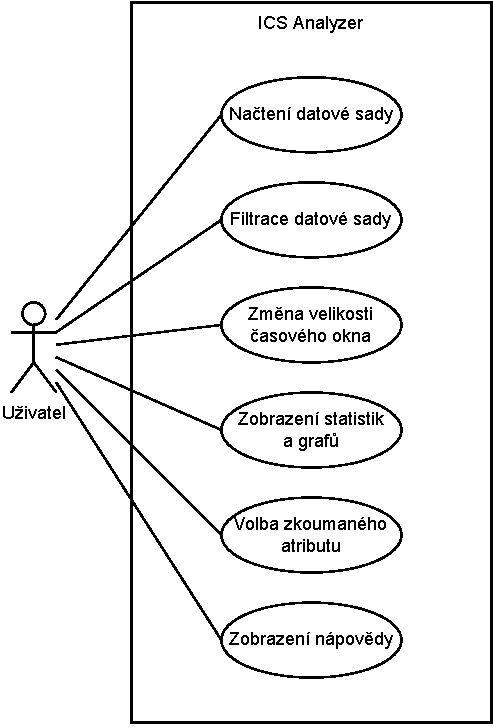
\includegraphics[width=0.6\textwidth]{obrazky-figures/use-case.pdf}
	\caption{Diagram případu užití (angl. \emph{use case}) demonstrující různé způsoby, kterými uživatel může interagovat s aplikací.}
	\label{fig:use-case}
\end{figure}



\section{Způsob zpracování dat}
\label{data_processing}


Důležitou součástí návrhu je způsob zpracování datové sady a to od jejího načtení po generování statistik a grafů. Aplikace bude pro manipulaci s daty na pozadí využívat knihovny \emph{Pandas} a její datové struktury zvané \uv{datový rámec} (angl. \emph{dataframe}, viz konec podkapitoly \ref{tools_and_libs}). Navržená sekvence zpracování je vyjádřena blokovým schématem na obrázku \ref{fig:block_diagram}. Její jednotlivé kroky jsou:

\begin{enumerate}
    \item \textbf{Načtení datového souboru:} v první řadě je potřeba datový soubor korektně načíst. Z dat obsažených v souboru v \emph{csv} formátu se vytvoří datový rámec, který jednotlivým atributům přiřadí datové typy. V tomto kroku je důležité, aby byly datové typy správně zvoleny, jinak načtení selže. Aplikace by měla provádět automatickou detekci datových typů a umožňovat uživateli jejich případnou změnu.
    \item \textbf{Převod do vnitřní reprezentace:} po načtení dat se do datového rámce přidají nové sloupce, které budou uživateli skryty a usnadní (programátorovi) další zpracování. Jedná se např. o sloupce pro označení stanic vnitřním identifikačním číslem apod.
    \item \textbf{Filtrování dat:} filtrace dat bude probíhat na základě pěti kritérií, které bude moct uživatel měnit. Datový rámec bude vyfiltrován tak, aby splňoval všechna nastavená kritéria. Výčet filtrů je uveden v podkapitole \ref{filters}.
    \item \textbf{Transformace dat na časová okna:} před zobrazením grafů bude potřeba data přetransformovat do podoby, která agreguje data do časových oken, jejichž velikost je volena uživatelem. Tato transformace je blíže popsána v sekci \ref{data_transformation}.
    \item \textbf{Sběr statistik:} ve chvíli kdy budou data vhodně předzpracována, bude možné začít generovat statistiky a grafy. Zatímco generování grafů očekává data již transformovaná na časová okna, některé statistiky tento krok vyžadovat nebudou. 
\end{enumerate}

\begin{figure}[H]
	\centering
	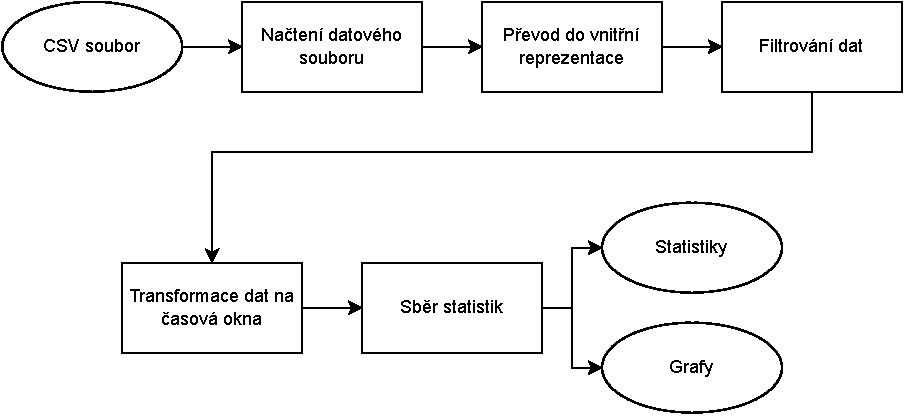
\includegraphics[width=1\textwidth]{obrazky-figures/block_diagram.pdf}
	\caption{Blokové schéma (angl. \emph{block diagram}) ukazující průběh zpracování datové sady.}
	\label{fig:block_diagram}
\end{figure}


\subsection{Filtrace datové sady}
\label{filters}

Aplikace bude nabízet celkově 5 kriterií, pomocí kterých bude možné filtrovat datovou sadu:

\begin{itemize}
        \item Adresa řídící stanice
        \item Adresy podřízených stanic
        \item Směr komunikace
        \item Začátek a konec komunikace (interval)
        \item Hodnoty zvoleného atributu
\end{itemize}


\subsection{Transformace dat na časová okna}
\label{data_transformation}

Pomocí transformace dat na časová okna lze z dat lépe získávat informaci o počtu zaznamenaných paketů s danou hodnotou atributu v daném intervale. V tabulce původních dat se nejprve vybere atribut, pro který se provede transformace. Aby měla transformace smysl, měl by atribut nabývat kategorických hodnot. Nemá smysl provádět transformaci pro spojité atributy (např. relativní čas), protože by se v nové tabulce objevovaly pouze záznamy (řádky) s jedinou nenulovou hodnotou. Následně se vytvoří nová tabulka, ve které jsou z jednotlivých hodnot vybraného atributu vytvořeny nové sloupce, které reprezentují absolutní četnost jejich zastoupení v časových oknech. Agregační funkcí je v tomto případě funkce \emph{počet}. Grafické znázornění transformace je ukázáno na obrázku \ref{fig:transformace_tabulky}.


\begin{figure}[H]
\centering
\begin{tikzpicture}
\node (A)
{
            \begin{tabularx}{0.6\textwidth}{|Y|c|c|c|}
            \hline
            \textbf{Začátek časového okna} & \textbf{a} & \textbf{b} & \textbf{c} \\ \hline
            17:50     & 1          & 2          & 0          \\ \hline
            17:55     & 1          & 0          & 0          \\ \hline
            18:00     & 3          & 0          & 0          \\ \hline
            18:05     & 0          & 1          & 1          \\ \hline
            \end{tabularx}
};
\node (B) [xshift=0cm, yshift={4.5cm}, at=(A)]
{
        \begin{tabularx}{0.6\textwidth}{|Y|c|}
            \hline
            \textbf{Časové razítko} & \textbf{Hodnota atributu} \\ \hline
            17:52:18       & a                \\ \hline
            17:52:24       & b                \\ \hline
            17:53:50       & b                \\ \hline
            \rowcolor[HTML]{EEEEEE}
            17:57:43       & a                \\ \hline
            18:01:17       & a                \\ \hline
            18:02:28       & a                \\ \hline
            18:02:45       & a                \\ \hline
            \rowcolor[HTML]{EEEEEE}
            18:06:33       & b                \\ \hline
            \rowcolor[HTML]{EEEEEE}
            18:06:42       & c                \\ \hline
            \end{tabularx}

};
\draw[->,ultra thick](B)--(A);
\end{tikzpicture}
\caption{Ukázka transformace dat na časová okna na náhodně vygenerovaných datech. Hodnoty atributu ($a$, $b$, $c$) byly vybrány pouze pro ilustrační účely. Velikost časového okna je 5 minut a agregační funkcí je funkce \emph{počet}.}
\label{fig:transformace_tabulky}
\end{figure}

\noindent \emph{Poznámka: Kromě funkce počet existují další široce užívané agregačních funkce. V případě, že atribut je číselného typu, lze použít např. funkce pro výpočet sumy, výpočet střední hodnoty, nalezení minima nebo maxima apod. Existuje i možnost vytvoření vlastní agregační funkce. V této práci je však využita pouze agregační funkce počet.}


\section{Uživatelské rozhraní}
\label{user_interface}

Uživatelské rozhraní aplikace se bude skládat z menu, informačního panelu a šesti karet. Společně tyto prvky budou tvořit přímočarý nástroj pro analýzu průmyslové komunikace.


\subsection*{Menu}

Menu bude hlavním prostředkem ovládání aplikace a bude nabízet 3 skupiny příkazů. Hierarchie příkazů a jejich funkcionalita je popsána výčtem:

\begin{enumerate}
    \item \textbf{File:} přikazy pro základní ovládání aplikace.
    \begin{itemize}
        \item \textbf{Load csv:} otevření dialogu pro načtení \texttt{csv} souboru. Načítání datové sady bude blíže popsáno v podkapitole \ref{dataset_loading}.
        \item \textbf{Exit:} ukončení aplikace.
    \end{itemize}
    
    \item \textbf{Filter:} příkazy pro filtraci datové sady.
    \begin{itemize}
        \item \textbf{Select master station:} otevření dialogu pro výběr řídící stanice.
        \item \textbf{Select slaves:} otevření dialogu pro výběr podmnožiny podřízených stanic. Výběr bude omezen na stanice, které komunikují s již zvolenou řídící stanicí.
        \item \textbf{Select direction:} otevření dialogu pro filtraci komunikace podle směru. Celkově budou k dispozici 3 druhy filtrace: obousměrná, M2S a S2M.
        \item \textbf{Change start and end time:} otevření dialogu pro omezení zkoumaného intervalu datové sady. Uživatel bude moct volit jeho začátek a konec.
        \item \textbf{Change time window size:} otevření dialogu pro změnu velikosti časového okna.
        \item \textbf{Select attribute:} otevření dialogu pro výběr atributu.
        \item \textbf{Select attribute values:} otevření dialogu pro výběr konkrétních hodnot již zvoleného atributu.
    \end{itemize}
    
    \item \textbf{Help:} příkazy nápovědy.
    \begin{itemize}
        \item \textbf{Show help:} zobrazení nápovědy.
        \item \textbf{About:} zobrazení základních informací o aplikaci.
    \end{itemize}
\end{enumerate}


\subsection*{Informační panel}


Informační panel by měl být vždy viditelným prvkem v horní části okna, který bude zobrazovat uživateli aktuálně aplikované nastavení a filtry datové sady. Konkrétně by měl zobrazovat nastavení filtrů pro adresu řídící stanice, adresy podřízených stanic, směr a časový interval. Panel by navíc měl ukazovat i nastavenou velikost časového okna a název zvoleného atributu.

\subsection*{Panel karet}

Stěžejním prvkem uživatelského rozhraní bude panel karet, který by měl nabízet uživateli celkově 6 různých pohledů na načtená data. Popis a význam jednotlivých pohledů je blíže rozebrán v podkapitole \ref{tab_views}. Jejich finální podoba je pak ukázána na obrázcích v příloze \ref{panel_images}.


\chapter{Implementace aplikace ICS Analyzer}
\label{chapter_implementation}

Následující kapitola se zabývá implementačními detaily aplikace \emph{ICS Analyzer}. K jejímu vývoji byl vybrán jazyk \emph{Python 3} a některé jeho široce užívané knihovny, jenž jsou představeny v podkapitole \ref{tools_and_libs}. Architektura aplikace a její rozdělení do logických celků je popsáno v podkapitole \ref{app_architecture}.

Během vývoje bylo potřeba vyřešit značné množství překážek. Jednou z nejvýznamnějších byla vysoká časová náročnost funkcí pro zpracování datových sad. Problém byl vyřešen použitím tzv. \emph{vektorizace}, která je popsána v podkapitole \ref{vectorization}.

Aplikace nabízí uživateli přímočarý způsob načítání datové sady. Jeho průběh je popsán v podkapitole \ref{dataset_loading}. Následuje představení jednotlivých pohledů (karet). Každý pohled nabízí unikátní náhled na datovou sadu a poskytuje uživateli jinou informaci o komunikaci. Jejich podrobný popis je uveden v podkapitole \ref{tab_views}.


\section{Použité nástroje a knihovny}
\label{tools_and_libs}

Implementace aplikace je založena na jazyce \emph{Python}\footnote{\url{https://www.python.org/downloads/release/python-3104/}} 3.10.4, který nabízí jak prostředky pro zpracování dat, tak pro tvorbu \emph{desktopových} aplikací a jejich uživatelského rozhraní. V implementaci jsou využity nové konstrukce verze 3.10 (např. \emph{structural pattern matching} nebo nová syntaxe pro \emph{type hinting}) a tudíž není aplikace zpětně kompatibilní se staršími verzemi.

K tvorbě grafického uživatelského rozhraní byla použita knihovna \emph{PyQt6}\footnote{\url{https://pypi.org/project/PyQt6/6.2.3/}}. Jedná se o~robustní a populární nástroj pro tvorbu multiplatformních uživatelských rozhraní, který vychází z frameworku \emph{Qt} pro \emph{C++}. \emph{PyQt6} poskytuje uživateli možnost tvorby rozhraní jak \uv{programově}, tak pomocí nástroje \emph{Qt Designer}. Pro účely této práce byla zvolena první varianta.

K načtení, zpracování a analýze datových sad byly využity knihovny \emph{NumPy}\footnote{\url{https://numpy.org/}} a \emph{Pandas}\footnote{\url{https://pandas.pydata.org/}}. Ke grafickému zobrazení dat pak byly použity knihovny \emph{Matplotlib}\footnote{\url{https://matplotlib.org/}} a \emph{Seaborn}\footnote{\url{https://seaborn.pydata.org/}}. Všechny zmíněné knihovny jsou široce využívány komunitou a patří mezi standardní nástroje pro zpracování a analýzu dat.

Za speciální zmínku stojí datová struktura \emph{datového rámce} (angl. \emph{dataframe}), která je obecně nejpoužívanějším objektem knihovny \emph{Pandas} \cite{df}. Jedná se o dvourozměrnou datovou strukturu, kde řádky reprezentují jednotlivé záznamy a~sloupce reprezentují atributy datové sady. Sloupce jsou určeny názvem a datovým typem. Povinným sloupcem je tzv. \uv{index}, který slouží k adresaci záznamů. V aplikaci se datové rámce využívají k uchovávání načtených dat a manipulaci s nimi.

\section{Architektura}
\label{app_architecture}

Zdrojový kód aplikace je rozdělen na dva logické celky, které jsou implementovány ve formě \emph{Python} balíčků. Prvním z nich je balíček \texttt{app}, jenž implementuje hlavní části aplikace jako je uživatelské rozhraní apod. Druhým je balíček \texttt{dsmanipulator}, který poskytuje nástroje ke zpracování datových rámců obsahující data z průmyslové komunikace. Architektura aplikace je naznačená blokovým schématem na obrázku \ref{fig:app_arch}.

\begin{figure}[H]
	\centering
	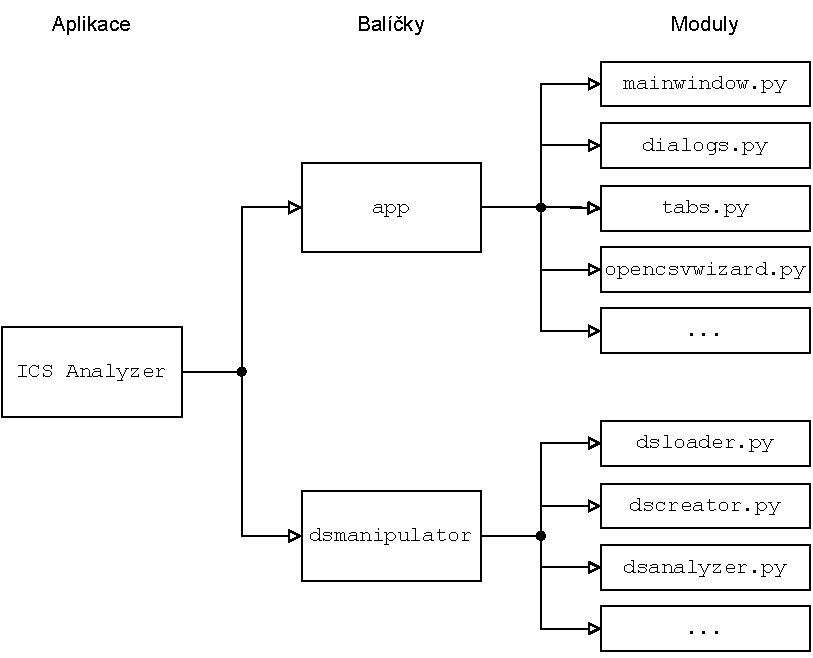
\includegraphics[width=0.8\textwidth]{obrazky-figures/architecture.pdf}
	\caption{Blokové schéma architektury aplikace \emph{ICS Analyzer}. Schéma obsahuje pouze nejdůležitější moduly.}
	\label{fig:app_arch}
\end{figure}




\subsection*{Balíček \texttt{app}}
\label{app}

Balíček obsahuje implementaci grafického uživatelského rozhraní a funkcionality aplikace. Využívá metod nabízených balíčkem \texttt{dsmanipulator}. Nejdůležitějšími moduly balíčku jsou:

\begin{itemize}
    \item \texttt{mainwindow}: implementace hlavního okna aplikace.
    \item \texttt{dialogs}: implementace dialogů aplikace (např. dialog pro změnu řídící stanice, intervalu, \dots).
    \item \texttt{tabs}: implementace pohledů (karet) aplikace. Jednotlivé pohledy jsou blíže popsány v podkapitole \ref{tab_views}.
    \item \texttt{opencsvwizard}: implementace dialogu pro načítání \texttt{csv} souborů, jehož podrobnější popis je uveden v podkapitole \ref{dataset_loading}.
\end{itemize}



\subsection*{Balíček \texttt{dsmanipulator}}
\label{dsmanipulator}

Balíček nabízí funkcionalitu pro načítání a zpracování datových rámců, které obsahují záznamy průmyslové komunikace. Je koncipován tak, aby byl použitelný i jako samostatná jednotka (např. pro \uv{ruční} analýzu datových sad v nástroji \emph{Jupyter Notebook}\footnote{\url{https://jupyter.org/}}). Stěžejními moduly balíčku \texttt{dsmanipulator} jsou:

\begin{itemize}
    \item \texttt{dsloader}: funkce pro detekci vlastností \texttt{csv} souboru (např. oddělovače sloupců) a jeho načtení.
    \item \texttt{dscreator}: funkce pro vnitřní zpracování datového rámce. Jedná se např. o funkce pro převod indexového sloupce na časovou řadu nebo přidání sloupců pro reprezentaci různých vlastností (vnitřní identifikátor stanice, komunikující dvojice, \emph{inter-arrival time} \dots).
    \item \texttt{dsanalyzer}: funkce pro analýzu datového rámce, generování statistik a grafů.
\end{itemize}






\section{Vektorizace}
\label{vectorization}

Jedním z problémů, které vznikly během vývoje aplikace (konkrétně modulu \texttt{dscreator}), byla nízká efektivita funkcí pro zpracování datových rámců, což znemožňovalo použití aplikace pro větší datové sady. Z tohoto důvodu je v implementaci aplikace využito tzv. \emph{vektorizace}, díky které lze významně urychlit výpočet některých operací nad datovými rámci. Metody vektorizace jsou nabízeny převážně knihovnou \emph{NumPy} a v aplikaci jsou primárně využity v modulu \texttt{dscreator}. Příklad užití vektorizace v aplikaci je ukázán na obrázku \ref{fig:vectorization}.

\begin{figure}[H]%
    \centering
    \begin{subfigure}{0.8\textwidth}
        \centering
        
        \begin{python}
def add_station_id(
    df: pd.DataFrame,
    station_ids: dict[Station, int],
) -> pd.DataFrame:

    df["SRC station id"] = df.apply(
        lambda row: station_ids[Station(row["srcIP"], row["srcPort"])],
        axis=1,
    )

    return df
        \end{python}
        \caption{Původní \uv{naivní} implementace, která nevyužívá vektorizace. Při zpracování datové sady D byl čas potřebný k vykonání funkce 18.6~s.}
        \label{fig:vectorization1}
    \end{subfigure}
    \par\medskip
    \begin{subfigure}{0.8\textwidth}
        \centering
        
        \begin{python}
def add_station_id_vectorized(
    df: pd.DataFrame,
    station_ids: dict[Station, int],
) -> pd.DataFrame:

    def get_station_id(ip, port):
        return station_ids[Station(ip, port)]

    get_station_id_vectorized = np.vectorize(get_station_id)

    # prevod sloupcu datoveho ramce do numpy poli
    srcIPs = df["srcIP"].values
    srcPorts = df["srcPort"].values

    df["SRC station id"] = get_station_id_vectorized(srcIPs, srcPorts)

    return df
        \end{python}
        
        
        \caption{Implementace využívající vektorizace. Při zpracování datové sady D byl čas potřebný k vykonání funkce 1.72~s.}
        \label{fig:vectorization2}
    \end{subfigure}
    \caption{Funkce \texttt{add\_station\_id} přidává do datového rámce nový sloupec s vnitřním identifikátorem zdrojové stanice. Pro každý záznam v datové sadě musí funkce nahlédnout do slovníku \texttt{station\_ids}. Díky vektorizaci, lze tuto operaci provádět paralelně a snížit potřebný čas pro vykonání funkce. Při zpracování datové sady D bylo dosaženo téměř 11násobného zrychlení (testováno v prostředí \emph{Jupyter Notebook}, systém: Zorin OS 15.3, CPU: Intel i7-8750H, RAM: 16~GB). \emph{Poznámka: Pro účely ukázky byla funkce oproti implementaci v aplikaci zjednodušena.}}%
    \label{fig:vectorization}%
\end{figure}




\section{Načítání datových sad}
\label{dataset_loading}

Aplikace podporuje načítání datových sad ze souborů ve formátu \texttt{csv}. Podmínkou je, aby soubor obsahoval kompletní záznamy některých povinných atributů. Konkrétně se jedná o~tyto atributy: Časové razítko, IP adresa zdrojové stanice, IP adresa cílové stanice. Pro optimální funkcionalitu aplikace by se v datové sadě měly nacházet i nepovinné atributy značící relativní čas, port zdrojové stanice a port cílové stanice. V případě, že některý z těchto atributů chybí, budou některé části aplikace omezeny. Bez specifikace portů, může automatická detekce řídící stanice selhat. Při chybějícím relativním čase, nebudou k dispozici popisné statistiky \emph{inter-arrival time}.

Po kliknutí na tlačítko pro načtení nové datové sady se uživateli zobrazí obrazovka pro výběr oddělovače dat, která je zobrazena na obrázku \ref{fig:delim_select_screen}. Aplikace se nejprve pokusí oddělovač detekovat sama a zobrazí uživateli názvy sloupců, které by vznikly použitím daného oddělovače. V případě, že detekce selže (např. když se v názvech sloupců nachází jiné znaky běžně používané jako oddělovače), může uživatel volbu změnit a aplikace mu zobrazí nové názvy sloupců.

Na další obrazovce (viz \ref{fig:type_select_screen}) volí uživatel datové typy sloupců a~sloupce, které náleží speciálním atributům jako je časové razítko, IP adresa atd. Mezi podporované datové typy patří: časové razítko, textový řetězec a číselná hodnota. I v tomto případě se aplikace snaží automaticky detekovat datové typy atributů a to na základě prvních 10~000 záznamů. Je však žádoucí, aby uživatel detekované datové typy překontroloval a upravil, jelikož špatně zvolený datový typ vede k selhání načtení datové sady. Jelikož byla aplikace stavěna primárně pro zpracování datových sad představených v kapitole \ref{datasets_analysis}, je detekce pro tyhle datové sady optimalizována a nevyžaduje zásah uživatele. Dále uživatel volí, které sloupce reprezentují speciální atributy. Celkově aplikace podporuje 6 speciálních atributů, z nichž 3 jsou povinné (časové razítko, IP adresa zdrojové stanice, IP adresa cílové stanice) a 3 nepovinné (relativní čas, port zdrojové stanice, port cílové stanice). 
Při jakékoliv změně konfigurace, provede aplikace její kontrolu. Nejprve dojde k ověření zda-li jsou zvolené datové typy sloupců kompatibilní s reprezentací atributů. Poté se aplikace pokusí na pozadí načíst 15~000 záznamů a ověřit, že nedošlo k problémům při načítání. Pokud aplikace nalezne problém, vypíše se upozornění a uživateli je znemožněno postupovat dále.







\section{Pohledy}
\label{tab_views}


Pohledy nabízí způsob, jakým efektivně zkoumat načtená data. Celkově aplikace podporuje 6 pohledů, které se liší informační hodnotou a~mění se na základě zvoleného nastavení a~filtrů. U každého pohledu je uvedeno, které nastavení jej ovlivňuje. Nadpisy sekcí v této podkapitole reflektují pojmenování pohledů v aplikaci.


\subsection*{Dataset table}

Prvním pohledem je jednoduché promítnutí načteného datového souboru do tabulky. Tabulka přehledně zobrazuje data načtená z \texttt{csv} a usnadňuje jejich čtení a prohlížení. Pro uživatele má největší význam ve chvíli, kdy už se v komunikaci orientuje a potřebuje zkontrolovat např. hodnoty atributů jednotlivých paketů, jejich přesné pořadí apod. Pohled reaguje pouze na změny filtrů a jeho ukázka je na obrázku \ref{fig:tab1}.

\subsection*{General statistics}

Druhý pohled souhrnně zobrazuje základní statistiky datového souboru. Dělí se na dva sloupce. Levý sloupec zobrazuje statistiky načtených dat bez aplikovaných filtrů a~mění se pouze při načtení nové datové sady. Pravý sloupec zobrazuje statistiky filtrovaných dat a~mění se při jakékoliv změně filtrů. Uživateli dává pohled základní představu o vlastnostech datové sady kterou zkoumá. Ve statistikách jsou obsažený informace jako např. délka časového intervalu dat, popisné míry inter-arrival time (jehož význam je popsán v podkapitole \ref{inter-arrival_time}), seznam unikátních hodnot atributů atd. Ukázka pohledu je na obrázku \ref{fig:tab2}.

\subsection*{All pairs}
Pohled obsahuje jeden graf pro každou komunikační dvojici v datové sadě, které jsou vždy zobrazeny všechny (nezávisle na filtrech). Grafy ukazují vývoj jak celkového počtu paketů v čase, tak pro každý směr zvlášť. Pohled pomáhá uživateli určit, která stanice je řídící a~ukazuje v jakých časech mezi sebou stanice komunikují. Metoda analýzy komunikace pomocí počtu paketů je popsána v podkapitole \ref{packet_counting}. Pohled reaguje pouze na změnu velikosti časového okna a na změnu intervalu, ostatní filtry pohled neovlivňují. Ukázka pohledu je k nalezení v příloze \ref{fig:tab3}.


\subsection*{Selected slaves}

Čtvrtý pohled poskytuje uživateli náhled na průběh komunikace řídící stanice s jednotlivými podřízenými stanicemi.V horní části pohledu se nachází spojnicový graf, který vychází z~metody popsané v podkapitole \ref{master-orinted_plot}. Pod grafem se nachází tabulka, která ukazuje přesné hodnoty hranic (viz \ref{tab:idk}). Ukázka pohledu je na obrázku \ref{fig:tab4}.

\begin{table}[H]
\centering
\begin{tabular}{|l|l|l|l|l|}
\hline
\textbf{\begin{tabular}[c]{@{}l@{}}Adresa podřízené\\ stanice\end{tabular}} & \textbf{\begin{tabular}[c]{@{}l@{}}Čas prvního\\ paketu\end{tabular}} & \textbf{\begin{tabular}[c]{@{}l@{}}Čas posledního\\ paketu\end{tabular}} & \textbf{\begin{tabular}[c]{@{}l@{}}Délka\\ trvání\end{tabular}} & \textbf{\begin{tabular}[c]{@{}l@{}}Počet\\ paketů\end{tabular}} \\ \hline
192.168.11.11:49784                                                         & 13:03:10.31                                                           & 13:20:03.94                                                              & 00:16:53.63                                                     & 9905                                                            \\ \hline
192.168.11.11:49830                                                         & 13:20:04.97                                                           & 13:29:26.00                                                              & 00:09:21.03                                                     & 3011                                                            \\ \hline
192.168.11.11:49849                                                         & 13:29:27.03                                                           & 17:56:31.33                                                              & 04:27:04.30                                                     & 91617                                                           \\ \hline
\end{tabular}
\caption{Ukázka tabulky na komunikaci z datové sady C. Řádky reprezentují vlastnosti komunikace řídící stanice \texttt{192.168.11.248:2404} s jednotlivými podřízenými stanicemi.}
\label{tab:idk}
\end{table}


\subsection*{Attribute table}

Pokud je uživatelem vybrán atribut, zobrazí se v tomto pohledu tabulka časových oken, jejíž podoba je naznačena v tabulce \ref{tab:attribute_table}. Pohled reaguje na všechna možná nastavení a jeho ukázka je v přílože \ref{fig:tab5}.

\begin{table}[H]
\centering
\renewcommand{\arraystretch}{1.5}
\begin{tabular}{|c|c|c|c|c|}
\hline
               & \textbf{46} & \textbf{67} & \textbf{82} & $\cdots$ \\ \hline
\textbf{17:15} & 75          & 46          & 0           &     \\ \hline
\textbf{17:20} & 25          & 60          & 2           &     \\ \hline
\textbf{17:25} & 24          & 73          & 0           &     \\ \hline
$\vdots$            &             &             &             &     \\ \hline
\end{tabular}
\renewcommand{\arraystretch}{1}
\caption{Ukázka tabulky časových oken na datech z datové sady A. Na vertikální \uv{ose} jsou vyznačeny začátky časových oken, na horizontální \uv{ose} jsou vyznačeny vybrané hodnoty atributu \emph{ipLen}. Vnitřní buňky tabulky značí počet odchycených paketů v daném intervalu s danou hodnotou atributu.}
\label{tab:attribute_table}
\end{table}

\subsection*{Attribute statistics}

Poslední pohled nabízí bližší pohled na vybraný zkoumaný atribut. Přímo vychází z metody popsané v podkapitole \ref{attribute_stability}. V horní části pohledu je vygenerován spojnicový graf, který ukazuje počty paketů v časových oknech pro každou ze zvolených hodnot zkoumaného atributu. V dolní části pohledu se nachází přehledová tabulka, která ukazuje pro každou hodnotu atributu některé jeho míry polohy a variability. Popisné charakteristiky jsou počítány z počtu zachycených paketů v jednotlivých časových oknech. Hlavička přehledové tabulky je demonstrována tabulkou \ref{tab:descriptive_table}. Pohled reaguje na všechna možná nastavení. Ukázka viz \ref{fig:tab6}.

\begin{table}[H]
\begin{tabularx}{\textwidth}{|Y|l|l|l|l|l|l|l|l|l|l|l|}
\hline
\begin{tabular}[c]{@{}l@{}}Attr.\\ value\end{tabular} & $\mu$    & $\sigma$ & $\sigma^2$ & $q_1$    & $q_2$    & $q_3$    & $IQR$    & $\mu -3 \sigma$ & $\mu +3 \sigma$ & \begin{tabular}[c]{@{}l@{}}Interval\\ size\end{tabular} & Outliers      \\ \hline
                                                        $\cdots$  & $\cdots$ & $\cdots$ & $\cdots$   & $\cdots$ & $\cdots$ & $\cdots$ & $\cdots$ & $\cdots$        & $\cdots$        & $\cdots$      & $\cdots$ \\ \hline
\end{tabularx}
\caption{Ukázka hlavičky přehledové tabulky. Sloupec \emph{Interval size} reprezentuje velikost rozdílu $(\mu + 3 \sigma) - (\mu - 3 \sigma)$ a sloupec \emph{Outliers} počet hodnot, které spadají mimo interval $3\sigma$.}
\label{tab:descriptive_table}
\end{table}




\chapter{Experimenty}
\label{chapter_experiments}


Cílem experimentů je ukázat, že lze aplikaci \emph{ICS Analyzer} využít k nalezení stabilních charakteristik a anomálií v komunikaci. Pro experimenty bude využita datová sada B, obsahující běžnou komunikaci (viz \ref{basic_datasets}), a 6 datových sad s útoky, jejichž popis je uveden v podkapitole \ref{attack_datasets}. V první řadě je potřeba v běžné komunikaci najít takové typy paketů, jejichž počet zachycení v čase vykazuje známky stability. Typy paketů budou rozlišovány pomocí různých hodnot jednotlivých atributů. Průběh výběru relevantních typů je popsán v podkapitole \ref{search_stability}. Dalším krokem je použití aplikace k detekci anomálií v datových sadách s útoky, ke které by ideálně měla být využita znalost stabilních charakteristik. Výsledky analýzy datových sad s útoky jsou uvedeny v podkapitole \ref{attack_search}.



\section{Hledání stabilních atributů}
\label{search_stability}

Stabilním atributem se v této práci rozumí konkrétní hodnota atributu, jejíž počty se v~jednotlivých časových oknech výrazně nemění. Pro stabilní atributy je typické, že hodnota jejich rozptylu není příliš velká. Je však problematické určit hraniční hodnotu rozptylu tak, aby se o atributu dalo říct, že je dostatečně stabilní. Tuhle hranici je většinou potřeba určit experimentálně.
Obecně lze požadavky na hledané atributy shrnout těmito body:


\begin{enumerate}
    \item \textbf{Nízký rozptyl:} atribut by neměl mít příliš vysoký rozptyl, jelikož detekce odlehlých hodnot je pak příliš benevolentní a nezachytí vše co by měla. Ideálně by interval $\langle{\mu-3\sigma,\mu+3\sigma}\rangle$ (dále jen \uv{interval $3\sigma$}) měl být co nejmenší, tak aby byl detekovatelný i malý výkyv hodnot.
    \item \textbf{Příslušnost k intervalu $3\sigma$:} v ideálním případě by do intervalu $3\sigma$ měly padnout všechny hodnoty z normální komunikace. Většinou je však nutné připustit i několik málo hodnot, které padnou mimo interval. V případě, že by už v běžné komunikaci padalo mnoho hodnot mimo interval $3\sigma$, vznikaly by v analýze falešné pozitivní hodnoty (tj. normální hodnoty označené jako anomálie).
    \item \textbf{Kladná hodnota spodní hranice intervalu $3\sigma$:} obecně není příliš vhodné volit atributy, které se pohybují příliš \uv{nízko} tzn. jejich střední hodnota se blíží nule. U~takových atributů je obtížné detekovat výpadky. Proto minimálním požadavkem je aby byla spodní hranice intervalu $3\sigma$ větší než 0.
\end{enumerate}

\noindent Dobrou praktikou je neomezovat se pouze na \uv{nejstabilnější} atribut v komunikaci, ale uvažovat i ty méně stabilní. Různé druhy útoků a anomálií mohou ovlivňovat různé atributy.

\subsection*{Nalezené stabilní atributy}

Pomocí aplikace \emph{ICS Analyzer} byly v datové sadě B nalezeny atributy, které splňují výše popsané požadavky. Tyto atributy, jejich střední hodnota, rozptyl a interval $3\sigma$ jsou uvedeny v tabulce \ref{tab:stable_attributes}. Mezi atributy \emph{ipLen} a \emph{len} byla nalezena vysoká korelace, proto jsou jejich hodnoty v tabulce uvedeny společně. Dále budou tyto atributy označovány pojmem \uv{nalezené stabilní atributy}.

\begin{table}[H]
\centering
\begin{tabularx}{\textwidth}{|X|c|c|c|c|c|c|c|}
\hline
Atribut              & \begin{tabular}[c]{@{}c@{}}Hodnota\\ Atributu\end{tabular} & \begin{tabular}[c]{@{}c@{}}Směr\\ komunikace\end{tabular} & $\mu$                  & $\sigma$              & $\mu-3\sigma$          & $\mu+3\sigma$          & \begin{tabular}[c]{@{}c@{}}Velikost\\ intervalu $3\sigma$\end{tabular} \\ \hline
\multirow{2}{*}{fmt} & \multirow{2}{*}{0x01}                                      & obousměrná                                                & \multirow{2}{*}{19.54} & \multirow{2}{*}{2.43} & \multirow{2}{*}{12.27} & \multirow{2}{*}{26.82} & \multirow{2}{*}{14.55}                                                 \\ \cline{3-3}
                     &                                                            & \multicolumn{1}{l|}{S2M}                                  &                        &                       &                        &                        &                                                                        \\ \hline
ipLen                & 46                                                         & \multirow{2}{*}{obousměrná}                               & \multirow{2}{*}{26.10} & \multirow{2}{*}{2.59} & \multirow{2}{*}{18.33} & \multirow{2}{*}{33.87} & \multirow{2}{*}{15.53}                                                 \\ \cline{1-2}
len                  & 4                                                          &                                                           &                        &                       &                        &                        &                                                                        \\ \hline
ipLen                & 46                                                         & \multirow{2}{*}{S2M}                                      & \multirow{2}{*}{22.82} & \multirow{2}{*}{1.14} & \multirow{2}{*}{19.41} & \multirow{2}{*}{26.23} & \multirow{2}{*}{6.82}                                                  \\ \cline{1-2}
len                  & 4                                                          &                                                           &                        &                       &                        &                        &                                                                        \\ \hline
\end{tabularx}
\caption{Nalezené atributy vykazující stabilitu a jejich základní popisné charakteristiky.}
\label{tab:stable_attributes}
\end{table}



\section{Detekce útoků na dostupných sadách}
\label{attack_search}


Tato podkapitola se zabývá použitím aplikace \emph{ICS Analyzer} k detekci útoků v datových sadách z podkapitoly \ref{attack_datasets}. K nalezeným stabilním atributům z podkapitoly \ref{search_stability} je v experimentech věnována zvýšená pozornost. Není však pravidlem, že by díky těmto atributům bylo vždy možné jednoznačně detekovat útok. Všechny grafy v této podkapitole jsou vygenerovány aplikací \emph{ICS Analyzer} s velikostí časového okna 5 minut a pro obousměrnou komunikaci.



\subsection*{Datová sada \texttt{connection-loss.csv}}

Výpadek komunikace je velmi snadno odhalitelný již z grafu ukazující počet paketů v čase. Takový graf je dostupný v pohledu \emph{All pairs} (je jen jeden, protože se v komunikaci nachází pouze jedna komunikační dvojice) a jeho podoba je ukázána na obrázku \ref{fig:conn_loss_attack}.

Dalším ukazatelem, který napovídá tomu, že v komunikaci došlo k výpadku, je vysoká maximální hodnota \emph{inter-arrival time}, která je dle statistik aplikace 3637,29~s (údaj je dostupný v pohledu \emph{General statistics}).


\begin{figure}[H]
	\centering
    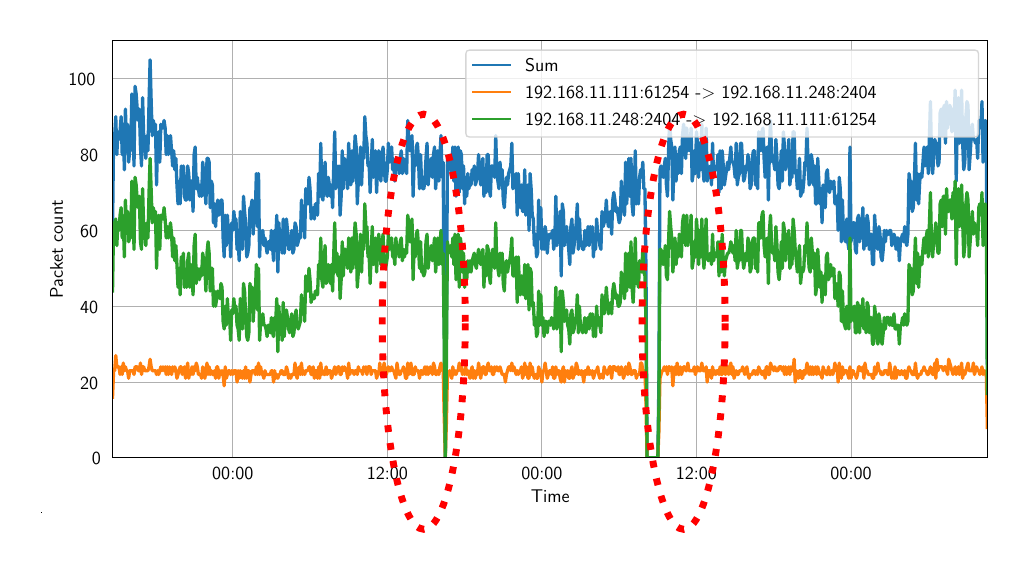
\begin{tikzpicture}
    \node(A){
    \resizebox{1\textwidth}{!}
        {
            %% Creator: Matplotlib, PGF backend
%%
%% To include the figure in your LaTeX document, write
%%   \input{<filename>.pgf}
%%
%% Make sure the required packages are loaded in your preamble
%%   \usepackage{pgf}
%%
%% Also ensure that all the required font packages are loaded; for instance,
%% the lmodern package is sometimes necessary when using math font.
%%   \usepackage{lmodern}
%%
%% Figures using additional raster images can only be included by \input if
%% they are in the same directory as the main LaTeX file. For loading figures
%% from other directories you can use the `import` package
%%   \usepackage{import}
%%
%% and then include the figures with
%%   \import{<path to file>}{<filename>.pgf}
%%
%% Matplotlib used the following preamble
%%   \usepackage{fontspec}
%%   \setmainfont{DejaVuSerif.ttf}[Path=\detokenize{/home/ankimme/fit/ibt/env/lib/python3.10/site-packages/matplotlib/mpl-data/fonts/ttf/}]
%%   \setsansfont{DejaVuSans.ttf}[Path=\detokenize{/home/ankimme/fit/ibt/env/lib/python3.10/site-packages/matplotlib/mpl-data/fonts/ttf/}]
%%   \setmonofont{DejaVuSansMono.ttf}[Path=\detokenize{/home/ankimme/fit/ibt/env/lib/python3.10/site-packages/matplotlib/mpl-data/fonts/ttf/}]
%%
\begingroup%
\makeatletter%
\begin{pgfpicture}%
\pgfpathrectangle{\pgfpointorigin}{\pgfqpoint{10.000000in}{5.000000in}}%
\pgfusepath{use as bounding box, clip}%
\begin{pgfscope}%
\pgfsetbuttcap%
\pgfsetmiterjoin%
\pgfsetlinewidth{0.000000pt}%
\definecolor{currentstroke}{rgb}{1.000000,1.000000,1.000000}%
\pgfsetstrokecolor{currentstroke}%
\pgfsetstrokeopacity{0.000000}%
\pgfsetdash{}{0pt}%
\pgfpathmoveto{\pgfqpoint{0.000000in}{0.000000in}}%
\pgfpathlineto{\pgfqpoint{10.000000in}{0.000000in}}%
\pgfpathlineto{\pgfqpoint{10.000000in}{5.000000in}}%
\pgfpathlineto{\pgfqpoint{0.000000in}{5.000000in}}%
\pgfpathlineto{\pgfqpoint{0.000000in}{0.000000in}}%
\pgfpathclose%
\pgfusepath{}%
\end{pgfscope}%
\begin{pgfscope}%
\pgfsetbuttcap%
\pgfsetmiterjoin%
\definecolor{currentfill}{rgb}{1.000000,1.000000,1.000000}%
\pgfsetfillcolor{currentfill}%
\pgfsetlinewidth{0.000000pt}%
\definecolor{currentstroke}{rgb}{0.000000,0.000000,0.000000}%
\pgfsetstrokecolor{currentstroke}%
\pgfsetstrokeopacity{0.000000}%
\pgfsetdash{}{0pt}%
\pgfpathmoveto{\pgfqpoint{0.753760in}{0.570804in}}%
\pgfpathlineto{\pgfqpoint{9.958330in}{0.570804in}}%
\pgfpathlineto{\pgfqpoint{9.958330in}{4.958330in}}%
\pgfpathlineto{\pgfqpoint{0.753760in}{4.958330in}}%
\pgfpathlineto{\pgfqpoint{0.753760in}{0.570804in}}%
\pgfpathclose%
\pgfusepath{fill}%
\end{pgfscope}%
\begin{pgfscope}%
\pgfpathrectangle{\pgfqpoint{0.753760in}{0.570804in}}{\pgfqpoint{9.204570in}{4.387526in}}%
\pgfusepath{clip}%
\pgfsetrectcap%
\pgfsetroundjoin%
\pgfsetlinewidth{0.803000pt}%
\definecolor{currentstroke}{rgb}{0.690196,0.690196,0.690196}%
\pgfsetstrokecolor{currentstroke}%
\pgfsetdash{}{0pt}%
\pgfpathmoveto{\pgfqpoint{2.014728in}{0.570804in}}%
\pgfpathlineto{\pgfqpoint{2.014728in}{4.958330in}}%
\pgfusepath{stroke}%
\end{pgfscope}%
\begin{pgfscope}%
\pgfsetbuttcap%
\pgfsetroundjoin%
\definecolor{currentfill}{rgb}{0.000000,0.000000,0.000000}%
\pgfsetfillcolor{currentfill}%
\pgfsetlinewidth{0.803000pt}%
\definecolor{currentstroke}{rgb}{0.000000,0.000000,0.000000}%
\pgfsetstrokecolor{currentstroke}%
\pgfsetdash{}{0pt}%
\pgfsys@defobject{currentmarker}{\pgfqpoint{0.000000in}{-0.048611in}}{\pgfqpoint{0.000000in}{0.000000in}}{%
\pgfpathmoveto{\pgfqpoint{0.000000in}{0.000000in}}%
\pgfpathlineto{\pgfqpoint{0.000000in}{-0.048611in}}%
\pgfusepath{stroke,fill}%
}%
\begin{pgfscope}%
\pgfsys@transformshift{2.014728in}{0.570804in}%
\pgfsys@useobject{currentmarker}{}%
\end{pgfscope}%
\end{pgfscope}%
\begin{pgfscope}%
\definecolor{textcolor}{rgb}{0.000000,0.000000,0.000000}%
\pgfsetstrokecolor{textcolor}%
\pgfsetfillcolor{textcolor}%
\pgftext[x=2.014728in,y=0.473582in,,top]{\color{textcolor}\sffamily\fontsize{14.000000}{16.800000}\selectfont 00:00}%
\end{pgfscope}%
\begin{pgfscope}%
\pgfpathrectangle{\pgfqpoint{0.753760in}{0.570804in}}{\pgfqpoint{9.204570in}{4.387526in}}%
\pgfusepath{clip}%
\pgfsetrectcap%
\pgfsetroundjoin%
\pgfsetlinewidth{0.803000pt}%
\definecolor{currentstroke}{rgb}{0.690196,0.690196,0.690196}%
\pgfsetstrokecolor{currentstroke}%
\pgfsetdash{}{0pt}%
\pgfpathmoveto{\pgfqpoint{3.641053in}{0.570804in}}%
\pgfpathlineto{\pgfqpoint{3.641053in}{4.958330in}}%
\pgfusepath{stroke}%
\end{pgfscope}%
\begin{pgfscope}%
\pgfsetbuttcap%
\pgfsetroundjoin%
\definecolor{currentfill}{rgb}{0.000000,0.000000,0.000000}%
\pgfsetfillcolor{currentfill}%
\pgfsetlinewidth{0.803000pt}%
\definecolor{currentstroke}{rgb}{0.000000,0.000000,0.000000}%
\pgfsetstrokecolor{currentstroke}%
\pgfsetdash{}{0pt}%
\pgfsys@defobject{currentmarker}{\pgfqpoint{0.000000in}{-0.048611in}}{\pgfqpoint{0.000000in}{0.000000in}}{%
\pgfpathmoveto{\pgfqpoint{0.000000in}{0.000000in}}%
\pgfpathlineto{\pgfqpoint{0.000000in}{-0.048611in}}%
\pgfusepath{stroke,fill}%
}%
\begin{pgfscope}%
\pgfsys@transformshift{3.641053in}{0.570804in}%
\pgfsys@useobject{currentmarker}{}%
\end{pgfscope}%
\end{pgfscope}%
\begin{pgfscope}%
\definecolor{textcolor}{rgb}{0.000000,0.000000,0.000000}%
\pgfsetstrokecolor{textcolor}%
\pgfsetfillcolor{textcolor}%
\pgftext[x=3.641053in,y=0.473582in,,top]{\color{textcolor}\sffamily\fontsize{14.000000}{16.800000}\selectfont 12:00}%
\end{pgfscope}%
\begin{pgfscope}%
\pgfpathrectangle{\pgfqpoint{0.753760in}{0.570804in}}{\pgfqpoint{9.204570in}{4.387526in}}%
\pgfusepath{clip}%
\pgfsetrectcap%
\pgfsetroundjoin%
\pgfsetlinewidth{0.803000pt}%
\definecolor{currentstroke}{rgb}{0.690196,0.690196,0.690196}%
\pgfsetstrokecolor{currentstroke}%
\pgfsetdash{}{0pt}%
\pgfpathmoveto{\pgfqpoint{5.267377in}{0.570804in}}%
\pgfpathlineto{\pgfqpoint{5.267377in}{4.958330in}}%
\pgfusepath{stroke}%
\end{pgfscope}%
\begin{pgfscope}%
\pgfsetbuttcap%
\pgfsetroundjoin%
\definecolor{currentfill}{rgb}{0.000000,0.000000,0.000000}%
\pgfsetfillcolor{currentfill}%
\pgfsetlinewidth{0.803000pt}%
\definecolor{currentstroke}{rgb}{0.000000,0.000000,0.000000}%
\pgfsetstrokecolor{currentstroke}%
\pgfsetdash{}{0pt}%
\pgfsys@defobject{currentmarker}{\pgfqpoint{0.000000in}{-0.048611in}}{\pgfqpoint{0.000000in}{0.000000in}}{%
\pgfpathmoveto{\pgfqpoint{0.000000in}{0.000000in}}%
\pgfpathlineto{\pgfqpoint{0.000000in}{-0.048611in}}%
\pgfusepath{stroke,fill}%
}%
\begin{pgfscope}%
\pgfsys@transformshift{5.267377in}{0.570804in}%
\pgfsys@useobject{currentmarker}{}%
\end{pgfscope}%
\end{pgfscope}%
\begin{pgfscope}%
\definecolor{textcolor}{rgb}{0.000000,0.000000,0.000000}%
\pgfsetstrokecolor{textcolor}%
\pgfsetfillcolor{textcolor}%
\pgftext[x=5.267377in,y=0.473582in,,top]{\color{textcolor}\sffamily\fontsize{14.000000}{16.800000}\selectfont 00:00}%
\end{pgfscope}%
\begin{pgfscope}%
\pgfpathrectangle{\pgfqpoint{0.753760in}{0.570804in}}{\pgfqpoint{9.204570in}{4.387526in}}%
\pgfusepath{clip}%
\pgfsetrectcap%
\pgfsetroundjoin%
\pgfsetlinewidth{0.803000pt}%
\definecolor{currentstroke}{rgb}{0.690196,0.690196,0.690196}%
\pgfsetstrokecolor{currentstroke}%
\pgfsetdash{}{0pt}%
\pgfpathmoveto{\pgfqpoint{6.893702in}{0.570804in}}%
\pgfpathlineto{\pgfqpoint{6.893702in}{4.958330in}}%
\pgfusepath{stroke}%
\end{pgfscope}%
\begin{pgfscope}%
\pgfsetbuttcap%
\pgfsetroundjoin%
\definecolor{currentfill}{rgb}{0.000000,0.000000,0.000000}%
\pgfsetfillcolor{currentfill}%
\pgfsetlinewidth{0.803000pt}%
\definecolor{currentstroke}{rgb}{0.000000,0.000000,0.000000}%
\pgfsetstrokecolor{currentstroke}%
\pgfsetdash{}{0pt}%
\pgfsys@defobject{currentmarker}{\pgfqpoint{0.000000in}{-0.048611in}}{\pgfqpoint{0.000000in}{0.000000in}}{%
\pgfpathmoveto{\pgfqpoint{0.000000in}{0.000000in}}%
\pgfpathlineto{\pgfqpoint{0.000000in}{-0.048611in}}%
\pgfusepath{stroke,fill}%
}%
\begin{pgfscope}%
\pgfsys@transformshift{6.893702in}{0.570804in}%
\pgfsys@useobject{currentmarker}{}%
\end{pgfscope}%
\end{pgfscope}%
\begin{pgfscope}%
\definecolor{textcolor}{rgb}{0.000000,0.000000,0.000000}%
\pgfsetstrokecolor{textcolor}%
\pgfsetfillcolor{textcolor}%
\pgftext[x=6.893702in,y=0.473582in,,top]{\color{textcolor}\sffamily\fontsize{14.000000}{16.800000}\selectfont 12:00}%
\end{pgfscope}%
\begin{pgfscope}%
\pgfpathrectangle{\pgfqpoint{0.753760in}{0.570804in}}{\pgfqpoint{9.204570in}{4.387526in}}%
\pgfusepath{clip}%
\pgfsetrectcap%
\pgfsetroundjoin%
\pgfsetlinewidth{0.803000pt}%
\definecolor{currentstroke}{rgb}{0.690196,0.690196,0.690196}%
\pgfsetstrokecolor{currentstroke}%
\pgfsetdash{}{0pt}%
\pgfpathmoveto{\pgfqpoint{8.520027in}{0.570804in}}%
\pgfpathlineto{\pgfqpoint{8.520027in}{4.958330in}}%
\pgfusepath{stroke}%
\end{pgfscope}%
\begin{pgfscope}%
\pgfsetbuttcap%
\pgfsetroundjoin%
\definecolor{currentfill}{rgb}{0.000000,0.000000,0.000000}%
\pgfsetfillcolor{currentfill}%
\pgfsetlinewidth{0.803000pt}%
\definecolor{currentstroke}{rgb}{0.000000,0.000000,0.000000}%
\pgfsetstrokecolor{currentstroke}%
\pgfsetdash{}{0pt}%
\pgfsys@defobject{currentmarker}{\pgfqpoint{0.000000in}{-0.048611in}}{\pgfqpoint{0.000000in}{0.000000in}}{%
\pgfpathmoveto{\pgfqpoint{0.000000in}{0.000000in}}%
\pgfpathlineto{\pgfqpoint{0.000000in}{-0.048611in}}%
\pgfusepath{stroke,fill}%
}%
\begin{pgfscope}%
\pgfsys@transformshift{8.520027in}{0.570804in}%
\pgfsys@useobject{currentmarker}{}%
\end{pgfscope}%
\end{pgfscope}%
\begin{pgfscope}%
\definecolor{textcolor}{rgb}{0.000000,0.000000,0.000000}%
\pgfsetstrokecolor{textcolor}%
\pgfsetfillcolor{textcolor}%
\pgftext[x=8.520027in,y=0.473582in,,top]{\color{textcolor}\sffamily\fontsize{14.000000}{16.800000}\selectfont 00:00}%
\end{pgfscope}%
\begin{pgfscope}%
\definecolor{textcolor}{rgb}{0.000000,0.000000,0.000000}%
\pgfsetstrokecolor{textcolor}%
\pgfsetfillcolor{textcolor}%
\pgftext[x=5.356045in,y=0.229848in,,top]{\color{textcolor}\sffamily\fontsize{14.000000}{16.800000}\selectfont Time}%
\end{pgfscope}%
\begin{pgfscope}%
\pgfpathrectangle{\pgfqpoint{0.753760in}{0.570804in}}{\pgfqpoint{9.204570in}{4.387526in}}%
\pgfusepath{clip}%
\pgfsetrectcap%
\pgfsetroundjoin%
\pgfsetlinewidth{0.803000pt}%
\definecolor{currentstroke}{rgb}{0.690196,0.690196,0.690196}%
\pgfsetstrokecolor{currentstroke}%
\pgfsetdash{}{0pt}%
\pgfpathmoveto{\pgfqpoint{0.753760in}{0.570804in}}%
\pgfpathlineto{\pgfqpoint{9.958330in}{0.570804in}}%
\pgfusepath{stroke}%
\end{pgfscope}%
\begin{pgfscope}%
\pgfsetbuttcap%
\pgfsetroundjoin%
\definecolor{currentfill}{rgb}{0.000000,0.000000,0.000000}%
\pgfsetfillcolor{currentfill}%
\pgfsetlinewidth{0.803000pt}%
\definecolor{currentstroke}{rgb}{0.000000,0.000000,0.000000}%
\pgfsetstrokecolor{currentstroke}%
\pgfsetdash{}{0pt}%
\pgfsys@defobject{currentmarker}{\pgfqpoint{-0.048611in}{0.000000in}}{\pgfqpoint{-0.000000in}{0.000000in}}{%
\pgfpathmoveto{\pgfqpoint{-0.000000in}{0.000000in}}%
\pgfpathlineto{\pgfqpoint{-0.048611in}{0.000000in}}%
\pgfusepath{stroke,fill}%
}%
\begin{pgfscope}%
\pgfsys@transformshift{0.753760in}{0.570804in}%
\pgfsys@useobject{currentmarker}{}%
\end{pgfscope}%
\end{pgfscope}%
\begin{pgfscope}%
\definecolor{textcolor}{rgb}{0.000000,0.000000,0.000000}%
\pgfsetstrokecolor{textcolor}%
\pgfsetfillcolor{textcolor}%
\pgftext[x=0.532827in, y=0.496938in, left, base]{\color{textcolor}\sffamily\fontsize{14.000000}{16.800000}\selectfont 0}%
\end{pgfscope}%
\begin{pgfscope}%
\pgfpathrectangle{\pgfqpoint{0.753760in}{0.570804in}}{\pgfqpoint{9.204570in}{4.387526in}}%
\pgfusepath{clip}%
\pgfsetrectcap%
\pgfsetroundjoin%
\pgfsetlinewidth{0.803000pt}%
\definecolor{currentstroke}{rgb}{0.690196,0.690196,0.690196}%
\pgfsetstrokecolor{currentstroke}%
\pgfsetdash{}{0pt}%
\pgfpathmoveto{\pgfqpoint{0.753760in}{1.368536in}}%
\pgfpathlineto{\pgfqpoint{9.958330in}{1.368536in}}%
\pgfusepath{stroke}%
\end{pgfscope}%
\begin{pgfscope}%
\pgfsetbuttcap%
\pgfsetroundjoin%
\definecolor{currentfill}{rgb}{0.000000,0.000000,0.000000}%
\pgfsetfillcolor{currentfill}%
\pgfsetlinewidth{0.803000pt}%
\definecolor{currentstroke}{rgb}{0.000000,0.000000,0.000000}%
\pgfsetstrokecolor{currentstroke}%
\pgfsetdash{}{0pt}%
\pgfsys@defobject{currentmarker}{\pgfqpoint{-0.048611in}{0.000000in}}{\pgfqpoint{-0.000000in}{0.000000in}}{%
\pgfpathmoveto{\pgfqpoint{-0.000000in}{0.000000in}}%
\pgfpathlineto{\pgfqpoint{-0.048611in}{0.000000in}}%
\pgfusepath{stroke,fill}%
}%
\begin{pgfscope}%
\pgfsys@transformshift{0.753760in}{1.368536in}%
\pgfsys@useobject{currentmarker}{}%
\end{pgfscope}%
\end{pgfscope}%
\begin{pgfscope}%
\definecolor{textcolor}{rgb}{0.000000,0.000000,0.000000}%
\pgfsetstrokecolor{textcolor}%
\pgfsetfillcolor{textcolor}%
\pgftext[x=0.409115in, y=1.294670in, left, base]{\color{textcolor}\sffamily\fontsize{14.000000}{16.800000}\selectfont 20}%
\end{pgfscope}%
\begin{pgfscope}%
\pgfpathrectangle{\pgfqpoint{0.753760in}{0.570804in}}{\pgfqpoint{9.204570in}{4.387526in}}%
\pgfusepath{clip}%
\pgfsetrectcap%
\pgfsetroundjoin%
\pgfsetlinewidth{0.803000pt}%
\definecolor{currentstroke}{rgb}{0.690196,0.690196,0.690196}%
\pgfsetstrokecolor{currentstroke}%
\pgfsetdash{}{0pt}%
\pgfpathmoveto{\pgfqpoint{0.753760in}{2.166268in}}%
\pgfpathlineto{\pgfqpoint{9.958330in}{2.166268in}}%
\pgfusepath{stroke}%
\end{pgfscope}%
\begin{pgfscope}%
\pgfsetbuttcap%
\pgfsetroundjoin%
\definecolor{currentfill}{rgb}{0.000000,0.000000,0.000000}%
\pgfsetfillcolor{currentfill}%
\pgfsetlinewidth{0.803000pt}%
\definecolor{currentstroke}{rgb}{0.000000,0.000000,0.000000}%
\pgfsetstrokecolor{currentstroke}%
\pgfsetdash{}{0pt}%
\pgfsys@defobject{currentmarker}{\pgfqpoint{-0.048611in}{0.000000in}}{\pgfqpoint{-0.000000in}{0.000000in}}{%
\pgfpathmoveto{\pgfqpoint{-0.000000in}{0.000000in}}%
\pgfpathlineto{\pgfqpoint{-0.048611in}{0.000000in}}%
\pgfusepath{stroke,fill}%
}%
\begin{pgfscope}%
\pgfsys@transformshift{0.753760in}{2.166268in}%
\pgfsys@useobject{currentmarker}{}%
\end{pgfscope}%
\end{pgfscope}%
\begin{pgfscope}%
\definecolor{textcolor}{rgb}{0.000000,0.000000,0.000000}%
\pgfsetstrokecolor{textcolor}%
\pgfsetfillcolor{textcolor}%
\pgftext[x=0.409115in, y=2.092402in, left, base]{\color{textcolor}\sffamily\fontsize{14.000000}{16.800000}\selectfont 40}%
\end{pgfscope}%
\begin{pgfscope}%
\pgfpathrectangle{\pgfqpoint{0.753760in}{0.570804in}}{\pgfqpoint{9.204570in}{4.387526in}}%
\pgfusepath{clip}%
\pgfsetrectcap%
\pgfsetroundjoin%
\pgfsetlinewidth{0.803000pt}%
\definecolor{currentstroke}{rgb}{0.690196,0.690196,0.690196}%
\pgfsetstrokecolor{currentstroke}%
\pgfsetdash{}{0pt}%
\pgfpathmoveto{\pgfqpoint{0.753760in}{2.964000in}}%
\pgfpathlineto{\pgfqpoint{9.958330in}{2.964000in}}%
\pgfusepath{stroke}%
\end{pgfscope}%
\begin{pgfscope}%
\pgfsetbuttcap%
\pgfsetroundjoin%
\definecolor{currentfill}{rgb}{0.000000,0.000000,0.000000}%
\pgfsetfillcolor{currentfill}%
\pgfsetlinewidth{0.803000pt}%
\definecolor{currentstroke}{rgb}{0.000000,0.000000,0.000000}%
\pgfsetstrokecolor{currentstroke}%
\pgfsetdash{}{0pt}%
\pgfsys@defobject{currentmarker}{\pgfqpoint{-0.048611in}{0.000000in}}{\pgfqpoint{-0.000000in}{0.000000in}}{%
\pgfpathmoveto{\pgfqpoint{-0.000000in}{0.000000in}}%
\pgfpathlineto{\pgfqpoint{-0.048611in}{0.000000in}}%
\pgfusepath{stroke,fill}%
}%
\begin{pgfscope}%
\pgfsys@transformshift{0.753760in}{2.964000in}%
\pgfsys@useobject{currentmarker}{}%
\end{pgfscope}%
\end{pgfscope}%
\begin{pgfscope}%
\definecolor{textcolor}{rgb}{0.000000,0.000000,0.000000}%
\pgfsetstrokecolor{textcolor}%
\pgfsetfillcolor{textcolor}%
\pgftext[x=0.409115in, y=2.890134in, left, base]{\color{textcolor}\sffamily\fontsize{14.000000}{16.800000}\selectfont 60}%
\end{pgfscope}%
\begin{pgfscope}%
\pgfpathrectangle{\pgfqpoint{0.753760in}{0.570804in}}{\pgfqpoint{9.204570in}{4.387526in}}%
\pgfusepath{clip}%
\pgfsetrectcap%
\pgfsetroundjoin%
\pgfsetlinewidth{0.803000pt}%
\definecolor{currentstroke}{rgb}{0.690196,0.690196,0.690196}%
\pgfsetstrokecolor{currentstroke}%
\pgfsetdash{}{0pt}%
\pgfpathmoveto{\pgfqpoint{0.753760in}{3.761732in}}%
\pgfpathlineto{\pgfqpoint{9.958330in}{3.761732in}}%
\pgfusepath{stroke}%
\end{pgfscope}%
\begin{pgfscope}%
\pgfsetbuttcap%
\pgfsetroundjoin%
\definecolor{currentfill}{rgb}{0.000000,0.000000,0.000000}%
\pgfsetfillcolor{currentfill}%
\pgfsetlinewidth{0.803000pt}%
\definecolor{currentstroke}{rgb}{0.000000,0.000000,0.000000}%
\pgfsetstrokecolor{currentstroke}%
\pgfsetdash{}{0pt}%
\pgfsys@defobject{currentmarker}{\pgfqpoint{-0.048611in}{0.000000in}}{\pgfqpoint{-0.000000in}{0.000000in}}{%
\pgfpathmoveto{\pgfqpoint{-0.000000in}{0.000000in}}%
\pgfpathlineto{\pgfqpoint{-0.048611in}{0.000000in}}%
\pgfusepath{stroke,fill}%
}%
\begin{pgfscope}%
\pgfsys@transformshift{0.753760in}{3.761732in}%
\pgfsys@useobject{currentmarker}{}%
\end{pgfscope}%
\end{pgfscope}%
\begin{pgfscope}%
\definecolor{textcolor}{rgb}{0.000000,0.000000,0.000000}%
\pgfsetstrokecolor{textcolor}%
\pgfsetfillcolor{textcolor}%
\pgftext[x=0.409115in, y=3.687866in, left, base]{\color{textcolor}\sffamily\fontsize{14.000000}{16.800000}\selectfont 80}%
\end{pgfscope}%
\begin{pgfscope}%
\pgfpathrectangle{\pgfqpoint{0.753760in}{0.570804in}}{\pgfqpoint{9.204570in}{4.387526in}}%
\pgfusepath{clip}%
\pgfsetrectcap%
\pgfsetroundjoin%
\pgfsetlinewidth{0.803000pt}%
\definecolor{currentstroke}{rgb}{0.690196,0.690196,0.690196}%
\pgfsetstrokecolor{currentstroke}%
\pgfsetdash{}{0pt}%
\pgfpathmoveto{\pgfqpoint{0.753760in}{4.559464in}}%
\pgfpathlineto{\pgfqpoint{9.958330in}{4.559464in}}%
\pgfusepath{stroke}%
\end{pgfscope}%
\begin{pgfscope}%
\pgfsetbuttcap%
\pgfsetroundjoin%
\definecolor{currentfill}{rgb}{0.000000,0.000000,0.000000}%
\pgfsetfillcolor{currentfill}%
\pgfsetlinewidth{0.803000pt}%
\definecolor{currentstroke}{rgb}{0.000000,0.000000,0.000000}%
\pgfsetstrokecolor{currentstroke}%
\pgfsetdash{}{0pt}%
\pgfsys@defobject{currentmarker}{\pgfqpoint{-0.048611in}{0.000000in}}{\pgfqpoint{-0.000000in}{0.000000in}}{%
\pgfpathmoveto{\pgfqpoint{-0.000000in}{0.000000in}}%
\pgfpathlineto{\pgfqpoint{-0.048611in}{0.000000in}}%
\pgfusepath{stroke,fill}%
}%
\begin{pgfscope}%
\pgfsys@transformshift{0.753760in}{4.559464in}%
\pgfsys@useobject{currentmarker}{}%
\end{pgfscope}%
\end{pgfscope}%
\begin{pgfscope}%
\definecolor{textcolor}{rgb}{0.000000,0.000000,0.000000}%
\pgfsetstrokecolor{textcolor}%
\pgfsetfillcolor{textcolor}%
\pgftext[x=0.285404in, y=4.485598in, left, base]{\color{textcolor}\sffamily\fontsize{14.000000}{16.800000}\selectfont 100}%
\end{pgfscope}%
\begin{pgfscope}%
\definecolor{textcolor}{rgb}{0.000000,0.000000,0.000000}%
\pgfsetstrokecolor{textcolor}%
\pgfsetfillcolor{textcolor}%
\pgftext[x=0.229848in,y=2.764567in,,bottom,rotate=90.000000]{\color{textcolor}\sffamily\fontsize{14.000000}{16.800000}\selectfont Packet count}%
\end{pgfscope}%
\begin{pgfscope}%
\pgfpathrectangle{\pgfqpoint{0.753760in}{0.570804in}}{\pgfqpoint{9.204570in}{4.387526in}}%
\pgfusepath{clip}%
\pgfsetrectcap%
\pgfsetroundjoin%
\pgfsetlinewidth{2.509375pt}%
\definecolor{currentstroke}{rgb}{0.121569,0.466667,0.705882}%
\pgfsetstrokecolor{currentstroke}%
\pgfsetdash{}{0pt}%
\pgfpathmoveto{\pgfqpoint{0.749808in}{2.964000in}}%
\pgfpathlineto{\pgfqpoint{0.761102in}{3.961165in}}%
\pgfpathlineto{\pgfqpoint{0.772396in}{3.961165in}}%
\pgfpathlineto{\pgfqpoint{0.783690in}{4.160598in}}%
\pgfpathlineto{\pgfqpoint{0.794984in}{3.761732in}}%
\pgfpathlineto{\pgfqpoint{0.806278in}{4.001052in}}%
\pgfpathlineto{\pgfqpoint{0.817572in}{3.921278in}}%
\pgfpathlineto{\pgfqpoint{0.828866in}{4.001052in}}%
\pgfpathlineto{\pgfqpoint{0.840160in}{4.160598in}}%
\pgfpathlineto{\pgfqpoint{0.851453in}{3.761732in}}%
\pgfpathlineto{\pgfqpoint{0.862747in}{4.080825in}}%
\pgfpathlineto{\pgfqpoint{0.874041in}{3.602186in}}%
\pgfpathlineto{\pgfqpoint{0.885335in}{4.240371in}}%
\pgfpathlineto{\pgfqpoint{0.896629in}{3.881392in}}%
\pgfpathlineto{\pgfqpoint{0.907923in}{4.080825in}}%
\pgfpathlineto{\pgfqpoint{0.919217in}{3.681959in}}%
\pgfpathlineto{\pgfqpoint{0.930511in}{3.801619in}}%
\pgfpathlineto{\pgfqpoint{0.941805in}{3.801619in}}%
\pgfpathlineto{\pgfqpoint{0.953099in}{4.399918in}}%
\pgfpathlineto{\pgfqpoint{0.964393in}{4.240371in}}%
\pgfpathlineto{\pgfqpoint{0.975687in}{3.642072in}}%
\pgfpathlineto{\pgfqpoint{0.986981in}{4.479691in}}%
\pgfpathlineto{\pgfqpoint{0.998274in}{4.399918in}}%
\pgfpathlineto{\pgfqpoint{1.009568in}{4.240371in}}%
\pgfpathlineto{\pgfqpoint{1.020862in}{4.120711in}}%
\pgfpathlineto{\pgfqpoint{1.032156in}{4.240371in}}%
\pgfpathlineto{\pgfqpoint{1.043450in}{3.841505in}}%
\pgfpathlineto{\pgfqpoint{1.054744in}{3.642072in}}%
\pgfpathlineto{\pgfqpoint{1.066038in}{4.360031in}}%
\pgfpathlineto{\pgfqpoint{1.077332in}{3.961165in}}%
\pgfpathlineto{\pgfqpoint{1.088626in}{3.881392in}}%
\pgfpathlineto{\pgfqpoint{1.099920in}{3.721845in}}%
\pgfpathlineto{\pgfqpoint{1.111214in}{3.961165in}}%
\pgfpathlineto{\pgfqpoint{1.122508in}{3.801619in}}%
\pgfpathlineto{\pgfqpoint{1.133802in}{4.320144in}}%
\pgfpathlineto{\pgfqpoint{1.145095in}{4.758897in}}%
\pgfpathlineto{\pgfqpoint{1.156389in}{4.320144in}}%
\pgfpathlineto{\pgfqpoint{1.167683in}{3.961165in}}%
\pgfpathlineto{\pgfqpoint{1.178977in}{4.120711in}}%
\pgfpathlineto{\pgfqpoint{1.190271in}{4.001052in}}%
\pgfpathlineto{\pgfqpoint{1.201565in}{4.080825in}}%
\pgfpathlineto{\pgfqpoint{1.212859in}{3.442639in}}%
\pgfpathlineto{\pgfqpoint{1.224153in}{3.921278in}}%
\pgfpathlineto{\pgfqpoint{1.235447in}{4.001052in}}%
\pgfpathlineto{\pgfqpoint{1.246741in}{3.681959in}}%
\pgfpathlineto{\pgfqpoint{1.258035in}{4.080825in}}%
\pgfpathlineto{\pgfqpoint{1.269329in}{4.040938in}}%
\pgfpathlineto{\pgfqpoint{1.280623in}{4.040938in}}%
\pgfpathlineto{\pgfqpoint{1.291916in}{4.120711in}}%
\pgfpathlineto{\pgfqpoint{1.303210in}{4.040938in}}%
\pgfpathlineto{\pgfqpoint{1.314504in}{3.761732in}}%
\pgfpathlineto{\pgfqpoint{1.325798in}{3.961165in}}%
\pgfpathlineto{\pgfqpoint{1.337092in}{3.761732in}}%
\pgfpathlineto{\pgfqpoint{1.348386in}{3.921278in}}%
\pgfpathlineto{\pgfqpoint{1.359680in}{3.961165in}}%
\pgfpathlineto{\pgfqpoint{1.382268in}{3.642072in}}%
\pgfpathlineto{\pgfqpoint{1.393562in}{3.801619in}}%
\pgfpathlineto{\pgfqpoint{1.404856in}{3.602186in}}%
\pgfpathlineto{\pgfqpoint{1.416150in}{3.721845in}}%
\pgfpathlineto{\pgfqpoint{1.427444in}{3.442639in}}%
\pgfpathlineto{\pgfqpoint{1.438737in}{3.243206in}}%
\pgfpathlineto{\pgfqpoint{1.450031in}{3.482526in}}%
\pgfpathlineto{\pgfqpoint{1.461325in}{3.243206in}}%
\pgfpathlineto{\pgfqpoint{1.472619in}{3.642072in}}%
\pgfpathlineto{\pgfqpoint{1.483913in}{3.442639in}}%
\pgfpathlineto{\pgfqpoint{1.495207in}{3.642072in}}%
\pgfpathlineto{\pgfqpoint{1.506501in}{3.322979in}}%
\pgfpathlineto{\pgfqpoint{1.517795in}{3.283093in}}%
\pgfpathlineto{\pgfqpoint{1.529089in}{3.283093in}}%
\pgfpathlineto{\pgfqpoint{1.540383in}{3.642072in}}%
\pgfpathlineto{\pgfqpoint{1.551677in}{3.562299in}}%
\pgfpathlineto{\pgfqpoint{1.562971in}{3.283093in}}%
\pgfpathlineto{\pgfqpoint{1.574265in}{3.482526in}}%
\pgfpathlineto{\pgfqpoint{1.585558in}{3.482526in}}%
\pgfpathlineto{\pgfqpoint{1.596852in}{3.163433in}}%
\pgfpathlineto{\pgfqpoint{1.608146in}{3.761732in}}%
\pgfpathlineto{\pgfqpoint{1.619440in}{3.841505in}}%
\pgfpathlineto{\pgfqpoint{1.630734in}{3.402753in}}%
\pgfpathlineto{\pgfqpoint{1.642028in}{3.522412in}}%
\pgfpathlineto{\pgfqpoint{1.653322in}{3.402753in}}%
\pgfpathlineto{\pgfqpoint{1.664616in}{3.322979in}}%
\pgfpathlineto{\pgfqpoint{1.675910in}{3.442639in}}%
\pgfpathlineto{\pgfqpoint{1.687204in}{3.322979in}}%
\pgfpathlineto{\pgfqpoint{1.698498in}{3.681959in}}%
\pgfpathlineto{\pgfqpoint{1.709792in}{3.562299in}}%
\pgfpathlineto{\pgfqpoint{1.732379in}{3.243206in}}%
\pgfpathlineto{\pgfqpoint{1.743673in}{3.721845in}}%
\pgfpathlineto{\pgfqpoint{1.754967in}{3.721845in}}%
\pgfpathlineto{\pgfqpoint{1.766261in}{3.681959in}}%
\pgfpathlineto{\pgfqpoint{1.777555in}{3.203320in}}%
\pgfpathlineto{\pgfqpoint{1.788849in}{3.482526in}}%
\pgfpathlineto{\pgfqpoint{1.800143in}{3.442639in}}%
\pgfpathlineto{\pgfqpoint{1.811437in}{3.043773in}}%
\pgfpathlineto{\pgfqpoint{1.822731in}{3.243206in}}%
\pgfpathlineto{\pgfqpoint{1.834025in}{3.003887in}}%
\pgfpathlineto{\pgfqpoint{1.845319in}{3.203320in}}%
\pgfpathlineto{\pgfqpoint{1.856613in}{3.283093in}}%
\pgfpathlineto{\pgfqpoint{1.867907in}{3.123546in}}%
\pgfpathlineto{\pgfqpoint{1.879200in}{3.163433in}}%
\pgfpathlineto{\pgfqpoint{1.890494in}{3.283093in}}%
\pgfpathlineto{\pgfqpoint{1.901788in}{3.283093in}}%
\pgfpathlineto{\pgfqpoint{1.913082in}{2.884227in}}%
\pgfpathlineto{\pgfqpoint{1.924376in}{2.684794in}}%
\pgfpathlineto{\pgfqpoint{1.935670in}{3.123546in}}%
\pgfpathlineto{\pgfqpoint{1.946964in}{2.804454in}}%
\pgfpathlineto{\pgfqpoint{1.958258in}{3.123546in}}%
\pgfpathlineto{\pgfqpoint{1.969552in}{2.924113in}}%
\pgfpathlineto{\pgfqpoint{1.980846in}{3.003887in}}%
\pgfpathlineto{\pgfqpoint{1.992140in}{2.684794in}}%
\pgfpathlineto{\pgfqpoint{2.003434in}{3.043773in}}%
\pgfpathlineto{\pgfqpoint{2.014728in}{2.964000in}}%
\pgfpathlineto{\pgfqpoint{2.026021in}{3.163433in}}%
\pgfpathlineto{\pgfqpoint{2.037315in}{3.043773in}}%
\pgfpathlineto{\pgfqpoint{2.048609in}{3.083660in}}%
\pgfpathlineto{\pgfqpoint{2.059903in}{2.764567in}}%
\pgfpathlineto{\pgfqpoint{2.071197in}{2.844340in}}%
\pgfpathlineto{\pgfqpoint{2.082491in}{2.644907in}}%
\pgfpathlineto{\pgfqpoint{2.093785in}{3.163433in}}%
\pgfpathlineto{\pgfqpoint{2.105079in}{2.924113in}}%
\pgfpathlineto{\pgfqpoint{2.116373in}{2.764567in}}%
\pgfpathlineto{\pgfqpoint{2.127667in}{3.322979in}}%
\pgfpathlineto{\pgfqpoint{2.138961in}{3.163433in}}%
\pgfpathlineto{\pgfqpoint{2.150255in}{3.043773in}}%
\pgfpathlineto{\pgfqpoint{2.161549in}{2.684794in}}%
\pgfpathlineto{\pgfqpoint{2.172842in}{2.724680in}}%
\pgfpathlineto{\pgfqpoint{2.184136in}{2.804454in}}%
\pgfpathlineto{\pgfqpoint{2.195430in}{3.203320in}}%
\pgfpathlineto{\pgfqpoint{2.206724in}{3.203320in}}%
\pgfpathlineto{\pgfqpoint{2.218018in}{3.283093in}}%
\pgfpathlineto{\pgfqpoint{2.229312in}{2.924113in}}%
\pgfpathlineto{\pgfqpoint{2.240606in}{3.123546in}}%
\pgfpathlineto{\pgfqpoint{2.251900in}{3.163433in}}%
\pgfpathlineto{\pgfqpoint{2.263194in}{3.562299in}}%
\pgfpathlineto{\pgfqpoint{2.274488in}{3.003887in}}%
\pgfpathlineto{\pgfqpoint{2.285782in}{3.562299in}}%
\pgfpathlineto{\pgfqpoint{2.297076in}{2.684794in}}%
\pgfpathlineto{\pgfqpoint{2.308370in}{2.964000in}}%
\pgfpathlineto{\pgfqpoint{2.319663in}{2.844340in}}%
\pgfpathlineto{\pgfqpoint{2.330957in}{2.964000in}}%
\pgfpathlineto{\pgfqpoint{2.342251in}{2.804454in}}%
\pgfpathlineto{\pgfqpoint{2.353545in}{2.884227in}}%
\pgfpathlineto{\pgfqpoint{2.376133in}{2.724680in}}%
\pgfpathlineto{\pgfqpoint{2.387427in}{2.844340in}}%
\pgfpathlineto{\pgfqpoint{2.398721in}{2.844340in}}%
\pgfpathlineto{\pgfqpoint{2.410015in}{2.764567in}}%
\pgfpathlineto{\pgfqpoint{2.421309in}{2.964000in}}%
\pgfpathlineto{\pgfqpoint{2.443897in}{2.644907in}}%
\pgfpathlineto{\pgfqpoint{2.455191in}{2.964000in}}%
\pgfpathlineto{\pgfqpoint{2.466485in}{2.844340in}}%
\pgfpathlineto{\pgfqpoint{2.477778in}{3.123546in}}%
\pgfpathlineto{\pgfqpoint{2.489072in}{2.525247in}}%
\pgfpathlineto{\pgfqpoint{2.500366in}{3.043773in}}%
\pgfpathlineto{\pgfqpoint{2.511660in}{2.764567in}}%
\pgfpathlineto{\pgfqpoint{2.522954in}{2.924113in}}%
\pgfpathlineto{\pgfqpoint{2.534248in}{2.724680in}}%
\pgfpathlineto{\pgfqpoint{2.545542in}{3.083660in}}%
\pgfpathlineto{\pgfqpoint{2.556836in}{2.724680in}}%
\pgfpathlineto{\pgfqpoint{2.568130in}{2.964000in}}%
\pgfpathlineto{\pgfqpoint{2.579424in}{3.083660in}}%
\pgfpathlineto{\pgfqpoint{2.590718in}{2.964000in}}%
\pgfpathlineto{\pgfqpoint{2.602012in}{2.764567in}}%
\pgfpathlineto{\pgfqpoint{2.613306in}{2.764567in}}%
\pgfpathlineto{\pgfqpoint{2.624599in}{2.844340in}}%
\pgfpathlineto{\pgfqpoint{2.635893in}{2.964000in}}%
\pgfpathlineto{\pgfqpoint{2.647187in}{2.724680in}}%
\pgfpathlineto{\pgfqpoint{2.658481in}{2.764567in}}%
\pgfpathlineto{\pgfqpoint{2.669775in}{3.043773in}}%
\pgfpathlineto{\pgfqpoint{2.681069in}{3.003887in}}%
\pgfpathlineto{\pgfqpoint{2.692363in}{2.804454in}}%
\pgfpathlineto{\pgfqpoint{2.703657in}{2.844340in}}%
\pgfpathlineto{\pgfqpoint{2.714951in}{2.924113in}}%
\pgfpathlineto{\pgfqpoint{2.726245in}{2.884227in}}%
\pgfpathlineto{\pgfqpoint{2.737539in}{3.283093in}}%
\pgfpathlineto{\pgfqpoint{2.748833in}{2.964000in}}%
\pgfpathlineto{\pgfqpoint{2.760127in}{3.163433in}}%
\pgfpathlineto{\pgfqpoint{2.771420in}{2.884227in}}%
\pgfpathlineto{\pgfqpoint{2.782714in}{3.402753in}}%
\pgfpathlineto{\pgfqpoint{2.805302in}{3.243206in}}%
\pgfpathlineto{\pgfqpoint{2.816596in}{3.522412in}}%
\pgfpathlineto{\pgfqpoint{2.827890in}{3.402753in}}%
\pgfpathlineto{\pgfqpoint{2.839184in}{3.083660in}}%
\pgfpathlineto{\pgfqpoint{2.850478in}{3.163433in}}%
\pgfpathlineto{\pgfqpoint{2.861772in}{3.203320in}}%
\pgfpathlineto{\pgfqpoint{2.873066in}{3.083660in}}%
\pgfpathlineto{\pgfqpoint{2.884360in}{3.243206in}}%
\pgfpathlineto{\pgfqpoint{2.895654in}{3.243206in}}%
\pgfpathlineto{\pgfqpoint{2.906948in}{3.123546in}}%
\pgfpathlineto{\pgfqpoint{2.918241in}{3.562299in}}%
\pgfpathlineto{\pgfqpoint{2.929535in}{3.322979in}}%
\pgfpathlineto{\pgfqpoint{2.940829in}{3.881392in}}%
\pgfpathlineto{\pgfqpoint{2.952123in}{3.322979in}}%
\pgfpathlineto{\pgfqpoint{2.963417in}{3.283093in}}%
\pgfpathlineto{\pgfqpoint{2.986005in}{3.681959in}}%
\pgfpathlineto{\pgfqpoint{2.997299in}{3.362866in}}%
\pgfpathlineto{\pgfqpoint{3.008593in}{3.322979in}}%
\pgfpathlineto{\pgfqpoint{3.019887in}{3.522412in}}%
\pgfpathlineto{\pgfqpoint{3.031181in}{3.442639in}}%
\pgfpathlineto{\pgfqpoint{3.042475in}{3.322979in}}%
\pgfpathlineto{\pgfqpoint{3.053769in}{3.442639in}}%
\pgfpathlineto{\pgfqpoint{3.065062in}{3.203320in}}%
\pgfpathlineto{\pgfqpoint{3.087650in}{4.001052in}}%
\pgfpathlineto{\pgfqpoint{3.098944in}{3.402753in}}%
\pgfpathlineto{\pgfqpoint{3.110238in}{3.642072in}}%
\pgfpathlineto{\pgfqpoint{3.121532in}{3.442639in}}%
\pgfpathlineto{\pgfqpoint{3.132826in}{3.642072in}}%
\pgfpathlineto{\pgfqpoint{3.144120in}{3.123546in}}%
\pgfpathlineto{\pgfqpoint{3.155414in}{3.322979in}}%
\pgfpathlineto{\pgfqpoint{3.166708in}{3.801619in}}%
\pgfpathlineto{\pgfqpoint{3.178002in}{3.402753in}}%
\pgfpathlineto{\pgfqpoint{3.189296in}{3.721845in}}%
\pgfpathlineto{\pgfqpoint{3.200590in}{3.681959in}}%
\pgfpathlineto{\pgfqpoint{3.211883in}{3.602186in}}%
\pgfpathlineto{\pgfqpoint{3.223177in}{3.402753in}}%
\pgfpathlineto{\pgfqpoint{3.234471in}{3.881392in}}%
\pgfpathlineto{\pgfqpoint{3.245765in}{3.562299in}}%
\pgfpathlineto{\pgfqpoint{3.257059in}{3.442639in}}%
\pgfpathlineto{\pgfqpoint{3.268353in}{3.801619in}}%
\pgfpathlineto{\pgfqpoint{3.279647in}{3.482526in}}%
\pgfpathlineto{\pgfqpoint{3.302235in}{3.961165in}}%
\pgfpathlineto{\pgfqpoint{3.313529in}{3.841505in}}%
\pgfpathlineto{\pgfqpoint{3.324823in}{3.243206in}}%
\pgfpathlineto{\pgfqpoint{3.336117in}{3.482526in}}%
\pgfpathlineto{\pgfqpoint{3.347411in}{3.642072in}}%
\pgfpathlineto{\pgfqpoint{3.358704in}{3.841505in}}%
\pgfpathlineto{\pgfqpoint{3.369998in}{3.442639in}}%
\pgfpathlineto{\pgfqpoint{3.381292in}{3.721845in}}%
\pgfpathlineto{\pgfqpoint{3.392586in}{3.721845in}}%
\pgfpathlineto{\pgfqpoint{3.403880in}{4.160598in}}%
\pgfpathlineto{\pgfqpoint{3.415174in}{3.961165in}}%
\pgfpathlineto{\pgfqpoint{3.426468in}{3.881392in}}%
\pgfpathlineto{\pgfqpoint{3.437762in}{3.642072in}}%
\pgfpathlineto{\pgfqpoint{3.449056in}{3.681959in}}%
\pgfpathlineto{\pgfqpoint{3.460350in}{3.362866in}}%
\pgfpathlineto{\pgfqpoint{3.482938in}{3.921278in}}%
\pgfpathlineto{\pgfqpoint{3.494232in}{3.522412in}}%
\pgfpathlineto{\pgfqpoint{3.505525in}{3.602186in}}%
\pgfpathlineto{\pgfqpoint{3.516819in}{3.801619in}}%
\pgfpathlineto{\pgfqpoint{3.528113in}{3.362866in}}%
\pgfpathlineto{\pgfqpoint{3.539407in}{3.642072in}}%
\pgfpathlineto{\pgfqpoint{3.550701in}{3.801619in}}%
\pgfpathlineto{\pgfqpoint{3.561995in}{3.761732in}}%
\pgfpathlineto{\pgfqpoint{3.573289in}{3.482526in}}%
\pgfpathlineto{\pgfqpoint{3.584583in}{3.721845in}}%
\pgfpathlineto{\pgfqpoint{3.595877in}{3.841505in}}%
\pgfpathlineto{\pgfqpoint{3.607171in}{3.642072in}}%
\pgfpathlineto{\pgfqpoint{3.618465in}{3.482526in}}%
\pgfpathlineto{\pgfqpoint{3.629759in}{3.482526in}}%
\pgfpathlineto{\pgfqpoint{3.641053in}{3.602186in}}%
\pgfpathlineto{\pgfqpoint{3.652346in}{3.881392in}}%
\pgfpathlineto{\pgfqpoint{3.663640in}{3.681959in}}%
\pgfpathlineto{\pgfqpoint{3.674934in}{3.721845in}}%
\pgfpathlineto{\pgfqpoint{3.686228in}{3.841505in}}%
\pgfpathlineto{\pgfqpoint{3.697522in}{3.602186in}}%
\pgfpathlineto{\pgfqpoint{3.708816in}{3.642072in}}%
\pgfpathlineto{\pgfqpoint{3.720110in}{3.482526in}}%
\pgfpathlineto{\pgfqpoint{3.731404in}{3.721845in}}%
\pgfpathlineto{\pgfqpoint{3.742698in}{3.721845in}}%
\pgfpathlineto{\pgfqpoint{3.753992in}{3.681959in}}%
\pgfpathlineto{\pgfqpoint{3.765286in}{3.562299in}}%
\pgfpathlineto{\pgfqpoint{3.776580in}{3.721845in}}%
\pgfpathlineto{\pgfqpoint{3.787874in}{3.801619in}}%
\pgfpathlineto{\pgfqpoint{3.799167in}{3.562299in}}%
\pgfpathlineto{\pgfqpoint{3.810461in}{3.721845in}}%
\pgfpathlineto{\pgfqpoint{3.821755in}{3.602186in}}%
\pgfpathlineto{\pgfqpoint{3.833049in}{3.602186in}}%
\pgfpathlineto{\pgfqpoint{3.844343in}{3.562299in}}%
\pgfpathlineto{\pgfqpoint{3.855637in}{4.120711in}}%
\pgfpathlineto{\pgfqpoint{3.866931in}{3.921278in}}%
\pgfpathlineto{\pgfqpoint{3.878225in}{3.801619in}}%
\pgfpathlineto{\pgfqpoint{3.889519in}{3.841505in}}%
\pgfpathlineto{\pgfqpoint{3.900813in}{3.961165in}}%
\pgfpathlineto{\pgfqpoint{3.912107in}{3.322979in}}%
\pgfpathlineto{\pgfqpoint{3.923401in}{3.681959in}}%
\pgfpathlineto{\pgfqpoint{3.934695in}{3.642072in}}%
\pgfpathlineto{\pgfqpoint{3.945988in}{3.841505in}}%
\pgfpathlineto{\pgfqpoint{3.957282in}{3.881392in}}%
\pgfpathlineto{\pgfqpoint{3.968576in}{3.721845in}}%
\pgfpathlineto{\pgfqpoint{3.979870in}{3.402753in}}%
\pgfpathlineto{\pgfqpoint{3.991164in}{3.761732in}}%
\pgfpathlineto{\pgfqpoint{4.002458in}{3.442639in}}%
\pgfpathlineto{\pgfqpoint{4.013752in}{3.402753in}}%
\pgfpathlineto{\pgfqpoint{4.025046in}{3.402753in}}%
\pgfpathlineto{\pgfqpoint{4.036340in}{3.482526in}}%
\pgfpathlineto{\pgfqpoint{4.047634in}{3.721845in}}%
\pgfpathlineto{\pgfqpoint{4.058928in}{3.881392in}}%
\pgfpathlineto{\pgfqpoint{4.070222in}{3.442639in}}%
\pgfpathlineto{\pgfqpoint{4.081516in}{3.602186in}}%
\pgfpathlineto{\pgfqpoint{4.092809in}{3.681959in}}%
\pgfpathlineto{\pgfqpoint{4.104103in}{3.721845in}}%
\pgfpathlineto{\pgfqpoint{4.115397in}{3.522412in}}%
\pgfpathlineto{\pgfqpoint{4.126691in}{3.761732in}}%
\pgfpathlineto{\pgfqpoint{4.137985in}{3.841505in}}%
\pgfpathlineto{\pgfqpoint{4.149279in}{3.402753in}}%
\pgfpathlineto{\pgfqpoint{4.160573in}{3.562299in}}%
\pgfpathlineto{\pgfqpoint{4.171867in}{3.801619in}}%
\pgfpathlineto{\pgfqpoint{4.183161in}{3.482526in}}%
\pgfpathlineto{\pgfqpoint{4.194455in}{3.761732in}}%
\pgfpathlineto{\pgfqpoint{4.205749in}{3.961165in}}%
\pgfpathlineto{\pgfqpoint{4.217043in}{3.522412in}}%
\pgfpathlineto{\pgfqpoint{4.228337in}{3.681959in}}%
\pgfpathlineto{\pgfqpoint{4.250924in}{0.570804in}}%
\pgfpathlineto{\pgfqpoint{4.262218in}{1.887062in}}%
\pgfpathlineto{\pgfqpoint{4.273512in}{3.721845in}}%
\pgfpathlineto{\pgfqpoint{4.284806in}{3.602186in}}%
\pgfpathlineto{\pgfqpoint{4.296100in}{3.681959in}}%
\pgfpathlineto{\pgfqpoint{4.307394in}{3.681959in}}%
\pgfpathlineto{\pgfqpoint{4.318688in}{3.522412in}}%
\pgfpathlineto{\pgfqpoint{4.329982in}{3.841505in}}%
\pgfpathlineto{\pgfqpoint{4.341276in}{3.482526in}}%
\pgfpathlineto{\pgfqpoint{4.352570in}{3.841505in}}%
\pgfpathlineto{\pgfqpoint{4.363864in}{3.322979in}}%
\pgfpathlineto{\pgfqpoint{4.375158in}{3.562299in}}%
\pgfpathlineto{\pgfqpoint{4.386451in}{3.841505in}}%
\pgfpathlineto{\pgfqpoint{4.397745in}{3.362866in}}%
\pgfpathlineto{\pgfqpoint{4.409039in}{3.801619in}}%
\pgfpathlineto{\pgfqpoint{4.420333in}{3.761732in}}%
\pgfpathlineto{\pgfqpoint{4.431627in}{3.402753in}}%
\pgfpathlineto{\pgfqpoint{4.442921in}{3.642072in}}%
\pgfpathlineto{\pgfqpoint{4.454215in}{3.243206in}}%
\pgfpathlineto{\pgfqpoint{4.465509in}{3.522412in}}%
\pgfpathlineto{\pgfqpoint{4.476803in}{3.322979in}}%
\pgfpathlineto{\pgfqpoint{4.488097in}{3.562299in}}%
\pgfpathlineto{\pgfqpoint{4.499391in}{3.402753in}}%
\pgfpathlineto{\pgfqpoint{4.510685in}{3.482526in}}%
\pgfpathlineto{\pgfqpoint{4.521979in}{3.442639in}}%
\pgfpathlineto{\pgfqpoint{4.533272in}{3.602186in}}%
\pgfpathlineto{\pgfqpoint{4.544566in}{3.522412in}}%
\pgfpathlineto{\pgfqpoint{4.555860in}{3.642072in}}%
\pgfpathlineto{\pgfqpoint{4.567154in}{3.442639in}}%
\pgfpathlineto{\pgfqpoint{4.578448in}{3.482526in}}%
\pgfpathlineto{\pgfqpoint{4.589742in}{3.562299in}}%
\pgfpathlineto{\pgfqpoint{4.601036in}{3.761732in}}%
\pgfpathlineto{\pgfqpoint{4.623624in}{3.442639in}}%
\pgfpathlineto{\pgfqpoint{4.634918in}{3.602186in}}%
\pgfpathlineto{\pgfqpoint{4.646212in}{3.721845in}}%
\pgfpathlineto{\pgfqpoint{4.657506in}{3.322979in}}%
\pgfpathlineto{\pgfqpoint{4.668800in}{3.562299in}}%
\pgfpathlineto{\pgfqpoint{4.680093in}{3.362866in}}%
\pgfpathlineto{\pgfqpoint{4.691387in}{3.761732in}}%
\pgfpathlineto{\pgfqpoint{4.702681in}{3.761732in}}%
\pgfpathlineto{\pgfqpoint{4.713975in}{3.402753in}}%
\pgfpathlineto{\pgfqpoint{4.725269in}{3.322979in}}%
\pgfpathlineto{\pgfqpoint{4.736563in}{3.642072in}}%
\pgfpathlineto{\pgfqpoint{4.747857in}{3.642072in}}%
\pgfpathlineto{\pgfqpoint{4.759151in}{3.602186in}}%
\pgfpathlineto{\pgfqpoint{4.770445in}{3.522412in}}%
\pgfpathlineto{\pgfqpoint{4.781739in}{3.961165in}}%
\pgfpathlineto{\pgfqpoint{4.793033in}{3.562299in}}%
\pgfpathlineto{\pgfqpoint{4.815621in}{3.402753in}}%
\pgfpathlineto{\pgfqpoint{4.826914in}{3.681959in}}%
\pgfpathlineto{\pgfqpoint{4.838208in}{3.442639in}}%
\pgfpathlineto{\pgfqpoint{4.849502in}{3.602186in}}%
\pgfpathlineto{\pgfqpoint{4.860796in}{3.283093in}}%
\pgfpathlineto{\pgfqpoint{4.872090in}{3.203320in}}%
\pgfpathlineto{\pgfqpoint{4.883384in}{3.402753in}}%
\pgfpathlineto{\pgfqpoint{4.894678in}{3.522412in}}%
\pgfpathlineto{\pgfqpoint{4.905972in}{3.442639in}}%
\pgfpathlineto{\pgfqpoint{4.917266in}{3.562299in}}%
\pgfpathlineto{\pgfqpoint{4.939854in}{3.642072in}}%
\pgfpathlineto{\pgfqpoint{4.951148in}{3.881392in}}%
\pgfpathlineto{\pgfqpoint{4.962442in}{3.402753in}}%
\pgfpathlineto{\pgfqpoint{4.985029in}{3.482526in}}%
\pgfpathlineto{\pgfqpoint{4.996323in}{3.562299in}}%
\pgfpathlineto{\pgfqpoint{5.007617in}{3.123546in}}%
\pgfpathlineto{\pgfqpoint{5.018911in}{3.562299in}}%
\pgfpathlineto{\pgfqpoint{5.030205in}{3.322979in}}%
\pgfpathlineto{\pgfqpoint{5.041499in}{3.203320in}}%
\pgfpathlineto{\pgfqpoint{5.052793in}{3.442639in}}%
\pgfpathlineto{\pgfqpoint{5.064087in}{3.163433in}}%
\pgfpathlineto{\pgfqpoint{5.075381in}{3.163433in}}%
\pgfpathlineto{\pgfqpoint{5.086675in}{3.602186in}}%
\pgfpathlineto{\pgfqpoint{5.097969in}{3.123546in}}%
\pgfpathlineto{\pgfqpoint{5.120556in}{3.442639in}}%
\pgfpathlineto{\pgfqpoint{5.131850in}{2.964000in}}%
\pgfpathlineto{\pgfqpoint{5.143144in}{3.562299in}}%
\pgfpathlineto{\pgfqpoint{5.154438in}{3.402753in}}%
\pgfpathlineto{\pgfqpoint{5.165732in}{3.123546in}}%
\pgfpathlineto{\pgfqpoint{5.177026in}{3.083660in}}%
\pgfpathlineto{\pgfqpoint{5.188320in}{2.804454in}}%
\pgfpathlineto{\pgfqpoint{5.199614in}{2.924113in}}%
\pgfpathlineto{\pgfqpoint{5.210908in}{2.684794in}}%
\pgfpathlineto{\pgfqpoint{5.222202in}{2.724680in}}%
\pgfpathlineto{\pgfqpoint{5.233496in}{3.283093in}}%
\pgfpathlineto{\pgfqpoint{5.244790in}{2.884227in}}%
\pgfpathlineto{\pgfqpoint{5.256084in}{3.203320in}}%
\pgfpathlineto{\pgfqpoint{5.267377in}{2.764567in}}%
\pgfpathlineto{\pgfqpoint{5.278671in}{2.964000in}}%
\pgfpathlineto{\pgfqpoint{5.289965in}{2.764567in}}%
\pgfpathlineto{\pgfqpoint{5.301259in}{3.003887in}}%
\pgfpathlineto{\pgfqpoint{5.312553in}{2.924113in}}%
\pgfpathlineto{\pgfqpoint{5.323847in}{2.724680in}}%
\pgfpathlineto{\pgfqpoint{5.335141in}{2.884227in}}%
\pgfpathlineto{\pgfqpoint{5.346435in}{2.924113in}}%
\pgfpathlineto{\pgfqpoint{5.357729in}{2.884227in}}%
\pgfpathlineto{\pgfqpoint{5.380317in}{2.964000in}}%
\pgfpathlineto{\pgfqpoint{5.391611in}{2.764567in}}%
\pgfpathlineto{\pgfqpoint{5.402905in}{2.844340in}}%
\pgfpathlineto{\pgfqpoint{5.414198in}{3.322979in}}%
\pgfpathlineto{\pgfqpoint{5.425492in}{2.804454in}}%
\pgfpathlineto{\pgfqpoint{5.436786in}{2.924113in}}%
\pgfpathlineto{\pgfqpoint{5.448080in}{3.003887in}}%
\pgfpathlineto{\pgfqpoint{5.459374in}{3.163433in}}%
\pgfpathlineto{\pgfqpoint{5.470668in}{2.485361in}}%
\pgfpathlineto{\pgfqpoint{5.481962in}{3.243206in}}%
\pgfpathlineto{\pgfqpoint{5.493256in}{3.163433in}}%
\pgfpathlineto{\pgfqpoint{5.504550in}{2.804454in}}%
\pgfpathlineto{\pgfqpoint{5.515844in}{2.964000in}}%
\pgfpathlineto{\pgfqpoint{5.527138in}{3.003887in}}%
\pgfpathlineto{\pgfqpoint{5.549726in}{2.764567in}}%
\pgfpathlineto{\pgfqpoint{5.561019in}{2.605021in}}%
\pgfpathlineto{\pgfqpoint{5.572313in}{3.003887in}}%
\pgfpathlineto{\pgfqpoint{5.583607in}{3.083660in}}%
\pgfpathlineto{\pgfqpoint{5.594901in}{2.724680in}}%
\pgfpathlineto{\pgfqpoint{5.606195in}{2.804454in}}%
\pgfpathlineto{\pgfqpoint{5.628783in}{3.043773in}}%
\pgfpathlineto{\pgfqpoint{5.640077in}{3.243206in}}%
\pgfpathlineto{\pgfqpoint{5.651371in}{2.764567in}}%
\pgfpathlineto{\pgfqpoint{5.662665in}{3.083660in}}%
\pgfpathlineto{\pgfqpoint{5.673959in}{2.804454in}}%
\pgfpathlineto{\pgfqpoint{5.685253in}{2.844340in}}%
\pgfpathlineto{\pgfqpoint{5.696547in}{2.764567in}}%
\pgfpathlineto{\pgfqpoint{5.707840in}{2.764567in}}%
\pgfpathlineto{\pgfqpoint{5.719134in}{2.964000in}}%
\pgfpathlineto{\pgfqpoint{5.730428in}{2.804454in}}%
\pgfpathlineto{\pgfqpoint{5.741722in}{2.844340in}}%
\pgfpathlineto{\pgfqpoint{5.753016in}{3.003887in}}%
\pgfpathlineto{\pgfqpoint{5.764310in}{2.804454in}}%
\pgfpathlineto{\pgfqpoint{5.775604in}{3.003887in}}%
\pgfpathlineto{\pgfqpoint{5.786898in}{2.844340in}}%
\pgfpathlineto{\pgfqpoint{5.798192in}{3.003887in}}%
\pgfpathlineto{\pgfqpoint{5.809486in}{2.684794in}}%
\pgfpathlineto{\pgfqpoint{5.820780in}{2.924113in}}%
\pgfpathlineto{\pgfqpoint{5.832074in}{2.764567in}}%
\pgfpathlineto{\pgfqpoint{5.843368in}{3.083660in}}%
\pgfpathlineto{\pgfqpoint{5.854662in}{2.924113in}}%
\pgfpathlineto{\pgfqpoint{5.865955in}{2.924113in}}%
\pgfpathlineto{\pgfqpoint{5.877249in}{2.804454in}}%
\pgfpathlineto{\pgfqpoint{5.888543in}{2.764567in}}%
\pgfpathlineto{\pgfqpoint{5.899837in}{3.163433in}}%
\pgfpathlineto{\pgfqpoint{5.911131in}{3.003887in}}%
\pgfpathlineto{\pgfqpoint{5.933719in}{3.083660in}}%
\pgfpathlineto{\pgfqpoint{5.945013in}{3.283093in}}%
\pgfpathlineto{\pgfqpoint{5.956307in}{3.083660in}}%
\pgfpathlineto{\pgfqpoint{5.967601in}{3.003887in}}%
\pgfpathlineto{\pgfqpoint{5.978895in}{3.123546in}}%
\pgfpathlineto{\pgfqpoint{5.990189in}{3.163433in}}%
\pgfpathlineto{\pgfqpoint{6.001483in}{2.924113in}}%
\pgfpathlineto{\pgfqpoint{6.012776in}{3.283093in}}%
\pgfpathlineto{\pgfqpoint{6.024070in}{3.362866in}}%
\pgfpathlineto{\pgfqpoint{6.035364in}{3.283093in}}%
\pgfpathlineto{\pgfqpoint{6.046658in}{3.163433in}}%
\pgfpathlineto{\pgfqpoint{6.057952in}{3.203320in}}%
\pgfpathlineto{\pgfqpoint{6.080540in}{3.043773in}}%
\pgfpathlineto{\pgfqpoint{6.091834in}{3.083660in}}%
\pgfpathlineto{\pgfqpoint{6.103128in}{3.482526in}}%
\pgfpathlineto{\pgfqpoint{6.114422in}{3.243206in}}%
\pgfpathlineto{\pgfqpoint{6.125716in}{3.203320in}}%
\pgfpathlineto{\pgfqpoint{6.137010in}{3.123546in}}%
\pgfpathlineto{\pgfqpoint{6.148304in}{3.681959in}}%
\pgfpathlineto{\pgfqpoint{6.159597in}{3.243206in}}%
\pgfpathlineto{\pgfqpoint{6.182185in}{3.721845in}}%
\pgfpathlineto{\pgfqpoint{6.193479in}{3.322979in}}%
\pgfpathlineto{\pgfqpoint{6.204773in}{3.721845in}}%
\pgfpathlineto{\pgfqpoint{6.216067in}{3.243206in}}%
\pgfpathlineto{\pgfqpoint{6.227361in}{3.123546in}}%
\pgfpathlineto{\pgfqpoint{6.238655in}{3.362866in}}%
\pgfpathlineto{\pgfqpoint{6.249949in}{3.801619in}}%
\pgfpathlineto{\pgfqpoint{6.261243in}{3.243206in}}%
\pgfpathlineto{\pgfqpoint{6.272537in}{3.322979in}}%
\pgfpathlineto{\pgfqpoint{6.283831in}{3.243206in}}%
\pgfpathlineto{\pgfqpoint{6.295125in}{3.522412in}}%
\pgfpathlineto{\pgfqpoint{6.306418in}{3.602186in}}%
\pgfpathlineto{\pgfqpoint{6.317712in}{3.522412in}}%
\pgfpathlineto{\pgfqpoint{6.329006in}{3.681959in}}%
\pgfpathlineto{\pgfqpoint{6.340300in}{3.402753in}}%
\pgfpathlineto{\pgfqpoint{6.351594in}{3.402753in}}%
\pgfpathlineto{\pgfqpoint{6.362888in}{2.525247in}}%
\pgfpathlineto{\pgfqpoint{6.374182in}{0.570804in}}%
\pgfpathlineto{\pgfqpoint{6.487121in}{0.570804in}}%
\pgfpathlineto{\pgfqpoint{6.498415in}{1.368536in}}%
\pgfpathlineto{\pgfqpoint{6.509709in}{3.602186in}}%
\pgfpathlineto{\pgfqpoint{6.521003in}{3.642072in}}%
\pgfpathlineto{\pgfqpoint{6.532297in}{3.562299in}}%
\pgfpathlineto{\pgfqpoint{6.543591in}{3.522412in}}%
\pgfpathlineto{\pgfqpoint{6.554885in}{3.642072in}}%
\pgfpathlineto{\pgfqpoint{6.566179in}{3.721845in}}%
\pgfpathlineto{\pgfqpoint{6.577473in}{3.442639in}}%
\pgfpathlineto{\pgfqpoint{6.588767in}{3.322979in}}%
\pgfpathlineto{\pgfqpoint{6.600060in}{3.801619in}}%
\pgfpathlineto{\pgfqpoint{6.611354in}{4.120711in}}%
\pgfpathlineto{\pgfqpoint{6.622648in}{3.921278in}}%
\pgfpathlineto{\pgfqpoint{6.633942in}{3.841505in}}%
\pgfpathlineto{\pgfqpoint{6.645236in}{3.283093in}}%
\pgfpathlineto{\pgfqpoint{6.656530in}{3.602186in}}%
\pgfpathlineto{\pgfqpoint{6.667824in}{3.841505in}}%
\pgfpathlineto{\pgfqpoint{6.679118in}{3.482526in}}%
\pgfpathlineto{\pgfqpoint{6.690412in}{3.761732in}}%
\pgfpathlineto{\pgfqpoint{6.701706in}{3.562299in}}%
\pgfpathlineto{\pgfqpoint{6.713000in}{3.801619in}}%
\pgfpathlineto{\pgfqpoint{6.724294in}{3.841505in}}%
\pgfpathlineto{\pgfqpoint{6.735588in}{3.562299in}}%
\pgfpathlineto{\pgfqpoint{6.746881in}{3.961165in}}%
\pgfpathlineto{\pgfqpoint{6.758175in}{4.080825in}}%
\pgfpathlineto{\pgfqpoint{6.769469in}{4.001052in}}%
\pgfpathlineto{\pgfqpoint{6.780763in}{3.721845in}}%
\pgfpathlineto{\pgfqpoint{6.792057in}{4.040938in}}%
\pgfpathlineto{\pgfqpoint{6.803351in}{3.801619in}}%
\pgfpathlineto{\pgfqpoint{6.814645in}{3.841505in}}%
\pgfpathlineto{\pgfqpoint{6.825939in}{3.801619in}}%
\pgfpathlineto{\pgfqpoint{6.837233in}{4.040938in}}%
\pgfpathlineto{\pgfqpoint{6.848527in}{3.482526in}}%
\pgfpathlineto{\pgfqpoint{6.859821in}{3.562299in}}%
\pgfpathlineto{\pgfqpoint{6.871115in}{3.801619in}}%
\pgfpathlineto{\pgfqpoint{6.882409in}{3.562299in}}%
\pgfpathlineto{\pgfqpoint{6.893702in}{4.001052in}}%
\pgfpathlineto{\pgfqpoint{6.904996in}{3.881392in}}%
\pgfpathlineto{\pgfqpoint{6.916290in}{3.522412in}}%
\pgfpathlineto{\pgfqpoint{6.927584in}{3.881392in}}%
\pgfpathlineto{\pgfqpoint{6.938878in}{3.602186in}}%
\pgfpathlineto{\pgfqpoint{6.950172in}{4.080825in}}%
\pgfpathlineto{\pgfqpoint{6.961466in}{3.642072in}}%
\pgfpathlineto{\pgfqpoint{6.972760in}{3.482526in}}%
\pgfpathlineto{\pgfqpoint{6.984054in}{3.721845in}}%
\pgfpathlineto{\pgfqpoint{6.995348in}{4.040938in}}%
\pgfpathlineto{\pgfqpoint{7.006642in}{3.482526in}}%
\pgfpathlineto{\pgfqpoint{7.017936in}{3.562299in}}%
\pgfpathlineto{\pgfqpoint{7.040523in}{3.642072in}}%
\pgfpathlineto{\pgfqpoint{7.051817in}{3.442639in}}%
\pgfpathlineto{\pgfqpoint{7.063111in}{3.881392in}}%
\pgfpathlineto{\pgfqpoint{7.074405in}{3.522412in}}%
\pgfpathlineto{\pgfqpoint{7.085699in}{3.642072in}}%
\pgfpathlineto{\pgfqpoint{7.096993in}{3.602186in}}%
\pgfpathlineto{\pgfqpoint{7.108287in}{3.602186in}}%
\pgfpathlineto{\pgfqpoint{7.119581in}{3.761732in}}%
\pgfpathlineto{\pgfqpoint{7.130875in}{3.362866in}}%
\pgfpathlineto{\pgfqpoint{7.142169in}{3.801619in}}%
\pgfpathlineto{\pgfqpoint{7.153463in}{3.402753in}}%
\pgfpathlineto{\pgfqpoint{7.164757in}{3.801619in}}%
\pgfpathlineto{\pgfqpoint{7.176051in}{3.642072in}}%
\pgfpathlineto{\pgfqpoint{7.187344in}{3.442639in}}%
\pgfpathlineto{\pgfqpoint{7.221226in}{3.681959in}}%
\pgfpathlineto{\pgfqpoint{7.232520in}{3.602186in}}%
\pgfpathlineto{\pgfqpoint{7.255108in}{3.841505in}}%
\pgfpathlineto{\pgfqpoint{7.266402in}{3.681959in}}%
\pgfpathlineto{\pgfqpoint{7.277696in}{3.681959in}}%
\pgfpathlineto{\pgfqpoint{7.288990in}{3.642072in}}%
\pgfpathlineto{\pgfqpoint{7.300284in}{3.522412in}}%
\pgfpathlineto{\pgfqpoint{7.311578in}{3.881392in}}%
\pgfpathlineto{\pgfqpoint{7.322872in}{3.442639in}}%
\pgfpathlineto{\pgfqpoint{7.334165in}{3.522412in}}%
\pgfpathlineto{\pgfqpoint{7.345459in}{3.562299in}}%
\pgfpathlineto{\pgfqpoint{7.356753in}{3.881392in}}%
\pgfpathlineto{\pgfqpoint{7.368047in}{3.881392in}}%
\pgfpathlineto{\pgfqpoint{7.379341in}{3.642072in}}%
\pgfpathlineto{\pgfqpoint{7.390635in}{3.482526in}}%
\pgfpathlineto{\pgfqpoint{7.401929in}{3.522412in}}%
\pgfpathlineto{\pgfqpoint{7.413223in}{3.642072in}}%
\pgfpathlineto{\pgfqpoint{7.424517in}{3.602186in}}%
\pgfpathlineto{\pgfqpoint{7.435811in}{3.761732in}}%
\pgfpathlineto{\pgfqpoint{7.447105in}{3.642072in}}%
\pgfpathlineto{\pgfqpoint{7.458399in}{3.402753in}}%
\pgfpathlineto{\pgfqpoint{7.469693in}{3.442639in}}%
\pgfpathlineto{\pgfqpoint{7.480986in}{3.721845in}}%
\pgfpathlineto{\pgfqpoint{7.492280in}{3.801619in}}%
\pgfpathlineto{\pgfqpoint{7.503574in}{3.801619in}}%
\pgfpathlineto{\pgfqpoint{7.514868in}{3.442639in}}%
\pgfpathlineto{\pgfqpoint{7.526162in}{3.562299in}}%
\pgfpathlineto{\pgfqpoint{7.537456in}{3.402753in}}%
\pgfpathlineto{\pgfqpoint{7.548750in}{4.001052in}}%
\pgfpathlineto{\pgfqpoint{7.560044in}{3.961165in}}%
\pgfpathlineto{\pgfqpoint{7.571338in}{3.801619in}}%
\pgfpathlineto{\pgfqpoint{7.582632in}{4.001052in}}%
\pgfpathlineto{\pgfqpoint{7.593926in}{4.040938in}}%
\pgfpathlineto{\pgfqpoint{7.605220in}{3.721845in}}%
\pgfpathlineto{\pgfqpoint{7.616514in}{3.522412in}}%
\pgfpathlineto{\pgfqpoint{7.627807in}{3.801619in}}%
\pgfpathlineto{\pgfqpoint{7.639101in}{3.841505in}}%
\pgfpathlineto{\pgfqpoint{7.650395in}{3.283093in}}%
\pgfpathlineto{\pgfqpoint{7.661689in}{3.841505in}}%
\pgfpathlineto{\pgfqpoint{7.672983in}{4.120711in}}%
\pgfpathlineto{\pgfqpoint{7.684277in}{3.761732in}}%
\pgfpathlineto{\pgfqpoint{7.695571in}{3.681959in}}%
\pgfpathlineto{\pgfqpoint{7.706865in}{3.681959in}}%
\pgfpathlineto{\pgfqpoint{7.718159in}{3.602186in}}%
\pgfpathlineto{\pgfqpoint{7.729453in}{3.921278in}}%
\pgfpathlineto{\pgfqpoint{7.740747in}{3.721845in}}%
\pgfpathlineto{\pgfqpoint{7.752041in}{3.442639in}}%
\pgfpathlineto{\pgfqpoint{7.763335in}{3.402753in}}%
\pgfpathlineto{\pgfqpoint{7.774628in}{3.522412in}}%
\pgfpathlineto{\pgfqpoint{7.785922in}{3.801619in}}%
\pgfpathlineto{\pgfqpoint{7.797216in}{3.482526in}}%
\pgfpathlineto{\pgfqpoint{7.808510in}{4.001052in}}%
\pgfpathlineto{\pgfqpoint{7.819804in}{3.841505in}}%
\pgfpathlineto{\pgfqpoint{7.831098in}{3.602186in}}%
\pgfpathlineto{\pgfqpoint{7.842392in}{3.801619in}}%
\pgfpathlineto{\pgfqpoint{7.853686in}{3.642072in}}%
\pgfpathlineto{\pgfqpoint{7.864980in}{3.921278in}}%
\pgfpathlineto{\pgfqpoint{7.876274in}{3.442639in}}%
\pgfpathlineto{\pgfqpoint{7.887568in}{3.562299in}}%
\pgfpathlineto{\pgfqpoint{7.898862in}{3.522412in}}%
\pgfpathlineto{\pgfqpoint{7.910156in}{4.001052in}}%
\pgfpathlineto{\pgfqpoint{7.921449in}{4.001052in}}%
\pgfpathlineto{\pgfqpoint{7.932743in}{3.562299in}}%
\pgfpathlineto{\pgfqpoint{7.944037in}{3.562299in}}%
\pgfpathlineto{\pgfqpoint{7.955331in}{3.402753in}}%
\pgfpathlineto{\pgfqpoint{7.966625in}{3.522412in}}%
\pgfpathlineto{\pgfqpoint{7.977919in}{3.721845in}}%
\pgfpathlineto{\pgfqpoint{7.989213in}{3.322979in}}%
\pgfpathlineto{\pgfqpoint{8.000507in}{3.362866in}}%
\pgfpathlineto{\pgfqpoint{8.011801in}{3.362866in}}%
\pgfpathlineto{\pgfqpoint{8.023095in}{3.482526in}}%
\pgfpathlineto{\pgfqpoint{8.034389in}{3.681959in}}%
\pgfpathlineto{\pgfqpoint{8.045683in}{3.681959in}}%
\pgfpathlineto{\pgfqpoint{8.056977in}{4.040938in}}%
\pgfpathlineto{\pgfqpoint{8.068270in}{3.642072in}}%
\pgfpathlineto{\pgfqpoint{8.079564in}{3.442639in}}%
\pgfpathlineto{\pgfqpoint{8.090858in}{3.482526in}}%
\pgfpathlineto{\pgfqpoint{8.102152in}{3.761732in}}%
\pgfpathlineto{\pgfqpoint{8.113446in}{3.681959in}}%
\pgfpathlineto{\pgfqpoint{8.124740in}{3.442639in}}%
\pgfpathlineto{\pgfqpoint{8.136034in}{3.642072in}}%
\pgfpathlineto{\pgfqpoint{8.147328in}{3.243206in}}%
\pgfpathlineto{\pgfqpoint{8.158622in}{3.243206in}}%
\pgfpathlineto{\pgfqpoint{8.169916in}{3.721845in}}%
\pgfpathlineto{\pgfqpoint{8.192504in}{3.243206in}}%
\pgfpathlineto{\pgfqpoint{8.203798in}{3.402753in}}%
\pgfpathlineto{\pgfqpoint{8.215091in}{3.043773in}}%
\pgfpathlineto{\pgfqpoint{8.226385in}{3.442639in}}%
\pgfpathlineto{\pgfqpoint{8.237679in}{3.362866in}}%
\pgfpathlineto{\pgfqpoint{8.248973in}{3.203320in}}%
\pgfpathlineto{\pgfqpoint{8.260267in}{3.562299in}}%
\pgfpathlineto{\pgfqpoint{8.271561in}{3.602186in}}%
\pgfpathlineto{\pgfqpoint{8.282855in}{3.402753in}}%
\pgfpathlineto{\pgfqpoint{8.294149in}{3.362866in}}%
\pgfpathlineto{\pgfqpoint{8.305443in}{3.482526in}}%
\pgfpathlineto{\pgfqpoint{8.316737in}{3.402753in}}%
\pgfpathlineto{\pgfqpoint{8.339325in}{3.482526in}}%
\pgfpathlineto{\pgfqpoint{8.350619in}{3.243206in}}%
\pgfpathlineto{\pgfqpoint{8.361912in}{3.322979in}}%
\pgfpathlineto{\pgfqpoint{8.373206in}{3.322979in}}%
\pgfpathlineto{\pgfqpoint{8.384500in}{2.964000in}}%
\pgfpathlineto{\pgfqpoint{8.395794in}{3.522412in}}%
\pgfpathlineto{\pgfqpoint{8.407088in}{3.402753in}}%
\pgfpathlineto{\pgfqpoint{8.418382in}{2.844340in}}%
\pgfpathlineto{\pgfqpoint{8.429676in}{3.283093in}}%
\pgfpathlineto{\pgfqpoint{8.440970in}{2.884227in}}%
\pgfpathlineto{\pgfqpoint{8.452264in}{2.884227in}}%
\pgfpathlineto{\pgfqpoint{8.463558in}{2.844340in}}%
\pgfpathlineto{\pgfqpoint{8.474852in}{3.083660in}}%
\pgfpathlineto{\pgfqpoint{8.486146in}{2.844340in}}%
\pgfpathlineto{\pgfqpoint{8.497440in}{2.764567in}}%
\pgfpathlineto{\pgfqpoint{8.508733in}{3.841505in}}%
\pgfpathlineto{\pgfqpoint{8.520027in}{2.844340in}}%
\pgfpathlineto{\pgfqpoint{8.531321in}{3.003887in}}%
\pgfpathlineto{\pgfqpoint{8.542615in}{3.043773in}}%
\pgfpathlineto{\pgfqpoint{8.553909in}{3.043773in}}%
\pgfpathlineto{\pgfqpoint{8.565203in}{2.764567in}}%
\pgfpathlineto{\pgfqpoint{8.576497in}{2.724680in}}%
\pgfpathlineto{\pgfqpoint{8.587791in}{3.083660in}}%
\pgfpathlineto{\pgfqpoint{8.599085in}{3.123546in}}%
\pgfpathlineto{\pgfqpoint{8.610379in}{2.844340in}}%
\pgfpathlineto{\pgfqpoint{8.621673in}{3.083660in}}%
\pgfpathlineto{\pgfqpoint{8.632967in}{2.884227in}}%
\pgfpathlineto{\pgfqpoint{8.644261in}{3.203320in}}%
\pgfpathlineto{\pgfqpoint{8.655554in}{2.764567in}}%
\pgfpathlineto{\pgfqpoint{8.666848in}{3.083660in}}%
\pgfpathlineto{\pgfqpoint{8.678142in}{2.804454in}}%
\pgfpathlineto{\pgfqpoint{8.689436in}{3.123546in}}%
\pgfpathlineto{\pgfqpoint{8.700730in}{3.043773in}}%
\pgfpathlineto{\pgfqpoint{8.712024in}{2.764567in}}%
\pgfpathlineto{\pgfqpoint{8.723318in}{2.924113in}}%
\pgfpathlineto{\pgfqpoint{8.734612in}{2.924113in}}%
\pgfpathlineto{\pgfqpoint{8.745906in}{2.605021in}}%
\pgfpathlineto{\pgfqpoint{8.757200in}{2.605021in}}%
\pgfpathlineto{\pgfqpoint{8.768494in}{3.123546in}}%
\pgfpathlineto{\pgfqpoint{8.779788in}{2.924113in}}%
\pgfpathlineto{\pgfqpoint{8.791082in}{2.804454in}}%
\pgfpathlineto{\pgfqpoint{8.802375in}{2.764567in}}%
\pgfpathlineto{\pgfqpoint{8.813669in}{3.003887in}}%
\pgfpathlineto{\pgfqpoint{8.824963in}{2.924113in}}%
\pgfpathlineto{\pgfqpoint{8.836257in}{2.684794in}}%
\pgfpathlineto{\pgfqpoint{8.847551in}{2.644907in}}%
\pgfpathlineto{\pgfqpoint{8.858845in}{2.764567in}}%
\pgfpathlineto{\pgfqpoint{8.870139in}{2.964000in}}%
\pgfpathlineto{\pgfqpoint{8.881433in}{2.844340in}}%
\pgfpathlineto{\pgfqpoint{8.892727in}{2.964000in}}%
\pgfpathlineto{\pgfqpoint{8.904021in}{2.924113in}}%
\pgfpathlineto{\pgfqpoint{8.915315in}{2.924113in}}%
\pgfpathlineto{\pgfqpoint{8.926609in}{2.964000in}}%
\pgfpathlineto{\pgfqpoint{8.937903in}{2.964000in}}%
\pgfpathlineto{\pgfqpoint{8.949196in}{2.804454in}}%
\pgfpathlineto{\pgfqpoint{8.960490in}{2.844340in}}%
\pgfpathlineto{\pgfqpoint{8.971784in}{2.924113in}}%
\pgfpathlineto{\pgfqpoint{8.983078in}{2.884227in}}%
\pgfpathlineto{\pgfqpoint{8.994372in}{2.764567in}}%
\pgfpathlineto{\pgfqpoint{9.005666in}{2.884227in}}%
\pgfpathlineto{\pgfqpoint{9.016960in}{2.884227in}}%
\pgfpathlineto{\pgfqpoint{9.028254in}{2.644907in}}%
\pgfpathlineto{\pgfqpoint{9.039548in}{2.844340in}}%
\pgfpathlineto{\pgfqpoint{9.062136in}{2.924113in}}%
\pgfpathlineto{\pgfqpoint{9.073430in}{2.844340in}}%
\pgfpathlineto{\pgfqpoint{9.084724in}{3.003887in}}%
\pgfpathlineto{\pgfqpoint{9.096017in}{2.844340in}}%
\pgfpathlineto{\pgfqpoint{9.107311in}{2.804454in}}%
\pgfpathlineto{\pgfqpoint{9.118605in}{2.924113in}}%
\pgfpathlineto{\pgfqpoint{9.129899in}{3.562299in}}%
\pgfpathlineto{\pgfqpoint{9.141193in}{3.482526in}}%
\pgfpathlineto{\pgfqpoint{9.152487in}{3.482526in}}%
\pgfpathlineto{\pgfqpoint{9.163781in}{3.163433in}}%
\pgfpathlineto{\pgfqpoint{9.175075in}{3.203320in}}%
\pgfpathlineto{\pgfqpoint{9.186369in}{3.482526in}}%
\pgfpathlineto{\pgfqpoint{9.197663in}{3.881392in}}%
\pgfpathlineto{\pgfqpoint{9.208957in}{3.283093in}}%
\pgfpathlineto{\pgfqpoint{9.220251in}{3.562299in}}%
\pgfpathlineto{\pgfqpoint{9.231545in}{3.243206in}}%
\pgfpathlineto{\pgfqpoint{9.242838in}{3.482526in}}%
\pgfpathlineto{\pgfqpoint{9.254132in}{3.562299in}}%
\pgfpathlineto{\pgfqpoint{9.265426in}{3.522412in}}%
\pgfpathlineto{\pgfqpoint{9.288014in}{3.841505in}}%
\pgfpathlineto{\pgfqpoint{9.299308in}{3.642072in}}%
\pgfpathlineto{\pgfqpoint{9.310602in}{3.801619in}}%
\pgfpathlineto{\pgfqpoint{9.321896in}{3.841505in}}%
\pgfpathlineto{\pgfqpoint{9.333190in}{3.562299in}}%
\pgfpathlineto{\pgfqpoint{9.355778in}{4.320144in}}%
\pgfpathlineto{\pgfqpoint{9.367072in}{3.721845in}}%
\pgfpathlineto{\pgfqpoint{9.378366in}{3.562299in}}%
\pgfpathlineto{\pgfqpoint{9.389660in}{3.721845in}}%
\pgfpathlineto{\pgfqpoint{9.400953in}{3.921278in}}%
\pgfpathlineto{\pgfqpoint{9.412247in}{3.881392in}}%
\pgfpathlineto{\pgfqpoint{9.423541in}{3.881392in}}%
\pgfpathlineto{\pgfqpoint{9.434835in}{3.642072in}}%
\pgfpathlineto{\pgfqpoint{9.446129in}{3.681959in}}%
\pgfpathlineto{\pgfqpoint{9.457423in}{4.200485in}}%
\pgfpathlineto{\pgfqpoint{9.468717in}{4.240371in}}%
\pgfpathlineto{\pgfqpoint{9.480011in}{3.961165in}}%
\pgfpathlineto{\pgfqpoint{9.491305in}{4.240371in}}%
\pgfpathlineto{\pgfqpoint{9.502599in}{4.280258in}}%
\pgfpathlineto{\pgfqpoint{9.513893in}{3.881392in}}%
\pgfpathlineto{\pgfqpoint{9.525187in}{4.320144in}}%
\pgfpathlineto{\pgfqpoint{9.536481in}{4.040938in}}%
\pgfpathlineto{\pgfqpoint{9.547774in}{4.200485in}}%
\pgfpathlineto{\pgfqpoint{9.559068in}{4.280258in}}%
\pgfpathlineto{\pgfqpoint{9.570362in}{4.240371in}}%
\pgfpathlineto{\pgfqpoint{9.581656in}{4.001052in}}%
\pgfpathlineto{\pgfqpoint{9.592950in}{4.240371in}}%
\pgfpathlineto{\pgfqpoint{9.604244in}{4.120711in}}%
\pgfpathlineto{\pgfqpoint{9.615538in}{4.439804in}}%
\pgfpathlineto{\pgfqpoint{9.626832in}{3.482526in}}%
\pgfpathlineto{\pgfqpoint{9.638126in}{4.120711in}}%
\pgfpathlineto{\pgfqpoint{9.649420in}{4.360031in}}%
\pgfpathlineto{\pgfqpoint{9.660714in}{3.881392in}}%
\pgfpathlineto{\pgfqpoint{9.672008in}{4.040938in}}%
\pgfpathlineto{\pgfqpoint{9.683302in}{4.439804in}}%
\pgfpathlineto{\pgfqpoint{9.694595in}{3.881392in}}%
\pgfpathlineto{\pgfqpoint{9.705889in}{3.602186in}}%
\pgfpathlineto{\pgfqpoint{9.717183in}{3.681959in}}%
\pgfpathlineto{\pgfqpoint{9.728477in}{4.160598in}}%
\pgfpathlineto{\pgfqpoint{9.739771in}{4.320144in}}%
\pgfpathlineto{\pgfqpoint{9.751065in}{4.280258in}}%
\pgfpathlineto{\pgfqpoint{9.762359in}{3.602186in}}%
\pgfpathlineto{\pgfqpoint{9.773653in}{3.761732in}}%
\pgfpathlineto{\pgfqpoint{9.784947in}{3.961165in}}%
\pgfpathlineto{\pgfqpoint{9.796241in}{4.080825in}}%
\pgfpathlineto{\pgfqpoint{9.807535in}{3.921278in}}%
\pgfpathlineto{\pgfqpoint{9.818829in}{3.921278in}}%
\pgfpathlineto{\pgfqpoint{9.830123in}{3.881392in}}%
\pgfpathlineto{\pgfqpoint{9.841416in}{3.921278in}}%
\pgfpathlineto{\pgfqpoint{9.852710in}{3.721845in}}%
\pgfpathlineto{\pgfqpoint{9.864004in}{4.120711in}}%
\pgfpathlineto{\pgfqpoint{9.875298in}{4.120711in}}%
\pgfpathlineto{\pgfqpoint{9.886592in}{4.040938in}}%
\pgfpathlineto{\pgfqpoint{9.897886in}{4.320144in}}%
\pgfpathlineto{\pgfqpoint{9.909180in}{3.681959in}}%
\pgfpathlineto{\pgfqpoint{9.920474in}{4.080825in}}%
\pgfpathlineto{\pgfqpoint{9.931768in}{4.120711in}}%
\pgfpathlineto{\pgfqpoint{9.943062in}{4.080825in}}%
\pgfpathlineto{\pgfqpoint{9.954356in}{1.567969in}}%
\pgfpathlineto{\pgfqpoint{9.954356in}{1.567969in}}%
\pgfusepath{stroke}%
\end{pgfscope}%
\begin{pgfscope}%
\pgfpathrectangle{\pgfqpoint{0.753760in}{0.570804in}}{\pgfqpoint{9.204570in}{4.387526in}}%
\pgfusepath{clip}%
\pgfsetrectcap%
\pgfsetroundjoin%
\pgfsetlinewidth{2.509375pt}%
\definecolor{currentstroke}{rgb}{1.000000,0.498039,0.054902}%
\pgfsetstrokecolor{currentstroke}%
\pgfsetdash{}{0pt}%
\pgfpathmoveto{\pgfqpoint{0.749808in}{1.208990in}}%
\pgfpathlineto{\pgfqpoint{0.761102in}{1.488196in}}%
\pgfpathlineto{\pgfqpoint{0.772396in}{1.488196in}}%
\pgfpathlineto{\pgfqpoint{0.783690in}{1.647742in}}%
\pgfpathlineto{\pgfqpoint{0.794984in}{1.528082in}}%
\pgfpathlineto{\pgfqpoint{0.817572in}{1.528082in}}%
\pgfpathlineto{\pgfqpoint{0.828866in}{1.448309in}}%
\pgfpathlineto{\pgfqpoint{0.840160in}{1.528082in}}%
\pgfpathlineto{\pgfqpoint{0.851453in}{1.448309in}}%
\pgfpathlineto{\pgfqpoint{0.862747in}{1.567969in}}%
\pgfpathlineto{\pgfqpoint{0.874041in}{1.488196in}}%
\pgfpathlineto{\pgfqpoint{0.885335in}{1.528082in}}%
\pgfpathlineto{\pgfqpoint{0.896629in}{1.488196in}}%
\pgfpathlineto{\pgfqpoint{0.907923in}{1.488196in}}%
\pgfpathlineto{\pgfqpoint{0.919217in}{1.408423in}}%
\pgfpathlineto{\pgfqpoint{0.930511in}{1.488196in}}%
\pgfpathlineto{\pgfqpoint{0.964393in}{1.488196in}}%
\pgfpathlineto{\pgfqpoint{0.975687in}{1.448309in}}%
\pgfpathlineto{\pgfqpoint{0.986981in}{1.528082in}}%
\pgfpathlineto{\pgfqpoint{1.009568in}{1.528082in}}%
\pgfpathlineto{\pgfqpoint{1.020862in}{1.488196in}}%
\pgfpathlineto{\pgfqpoint{1.032156in}{1.488196in}}%
\pgfpathlineto{\pgfqpoint{1.043450in}{1.567969in}}%
\pgfpathlineto{\pgfqpoint{1.054744in}{1.448309in}}%
\pgfpathlineto{\pgfqpoint{1.066038in}{1.528082in}}%
\pgfpathlineto{\pgfqpoint{1.077332in}{1.528082in}}%
\pgfpathlineto{\pgfqpoint{1.088626in}{1.488196in}}%
\pgfpathlineto{\pgfqpoint{1.122508in}{1.488196in}}%
\pgfpathlineto{\pgfqpoint{1.133802in}{1.528082in}}%
\pgfpathlineto{\pgfqpoint{1.145095in}{1.607856in}}%
\pgfpathlineto{\pgfqpoint{1.156389in}{1.528082in}}%
\pgfpathlineto{\pgfqpoint{1.167683in}{1.488196in}}%
\pgfpathlineto{\pgfqpoint{1.201565in}{1.488196in}}%
\pgfpathlineto{\pgfqpoint{1.212859in}{1.448309in}}%
\pgfpathlineto{\pgfqpoint{1.224153in}{1.488196in}}%
\pgfpathlineto{\pgfqpoint{1.235447in}{1.448309in}}%
\pgfpathlineto{\pgfqpoint{1.258035in}{1.528082in}}%
\pgfpathlineto{\pgfqpoint{1.269329in}{1.488196in}}%
\pgfpathlineto{\pgfqpoint{1.280623in}{1.528082in}}%
\pgfpathlineto{\pgfqpoint{1.291916in}{1.488196in}}%
\pgfpathlineto{\pgfqpoint{1.303210in}{1.528082in}}%
\pgfpathlineto{\pgfqpoint{1.314504in}{1.448309in}}%
\pgfpathlineto{\pgfqpoint{1.325798in}{1.528082in}}%
\pgfpathlineto{\pgfqpoint{1.337092in}{1.448309in}}%
\pgfpathlineto{\pgfqpoint{1.348386in}{1.528082in}}%
\pgfpathlineto{\pgfqpoint{1.370974in}{1.448309in}}%
\pgfpathlineto{\pgfqpoint{1.382268in}{1.528082in}}%
\pgfpathlineto{\pgfqpoint{1.393562in}{1.488196in}}%
\pgfpathlineto{\pgfqpoint{1.404856in}{1.528082in}}%
\pgfpathlineto{\pgfqpoint{1.416150in}{1.488196in}}%
\pgfpathlineto{\pgfqpoint{1.427444in}{1.408423in}}%
\pgfpathlineto{\pgfqpoint{1.461325in}{1.528082in}}%
\pgfpathlineto{\pgfqpoint{1.472619in}{1.528082in}}%
\pgfpathlineto{\pgfqpoint{1.483913in}{1.448309in}}%
\pgfpathlineto{\pgfqpoint{1.506501in}{1.528082in}}%
\pgfpathlineto{\pgfqpoint{1.517795in}{1.408423in}}%
\pgfpathlineto{\pgfqpoint{1.540383in}{1.567969in}}%
\pgfpathlineto{\pgfqpoint{1.551677in}{1.408423in}}%
\pgfpathlineto{\pgfqpoint{1.562971in}{1.488196in}}%
\pgfpathlineto{\pgfqpoint{1.574265in}{1.448309in}}%
\pgfpathlineto{\pgfqpoint{1.585558in}{1.528082in}}%
\pgfpathlineto{\pgfqpoint{1.596852in}{1.448309in}}%
\pgfpathlineto{\pgfqpoint{1.608146in}{1.528082in}}%
\pgfpathlineto{\pgfqpoint{1.619440in}{1.488196in}}%
\pgfpathlineto{\pgfqpoint{1.630734in}{1.567969in}}%
\pgfpathlineto{\pgfqpoint{1.642028in}{1.528082in}}%
\pgfpathlineto{\pgfqpoint{1.653322in}{1.448309in}}%
\pgfpathlineto{\pgfqpoint{1.675910in}{1.448309in}}%
\pgfpathlineto{\pgfqpoint{1.687204in}{1.408423in}}%
\pgfpathlineto{\pgfqpoint{1.698498in}{1.528082in}}%
\pgfpathlineto{\pgfqpoint{1.709792in}{1.488196in}}%
\pgfpathlineto{\pgfqpoint{1.721086in}{1.408423in}}%
\pgfpathlineto{\pgfqpoint{1.743673in}{1.567969in}}%
\pgfpathlineto{\pgfqpoint{1.754967in}{1.448309in}}%
\pgfpathlineto{\pgfqpoint{1.766261in}{1.528082in}}%
\pgfpathlineto{\pgfqpoint{1.777555in}{1.448309in}}%
\pgfpathlineto{\pgfqpoint{1.788849in}{1.488196in}}%
\pgfpathlineto{\pgfqpoint{1.800143in}{1.448309in}}%
\pgfpathlineto{\pgfqpoint{1.811437in}{1.448309in}}%
\pgfpathlineto{\pgfqpoint{1.822731in}{1.488196in}}%
\pgfpathlineto{\pgfqpoint{1.834025in}{1.408423in}}%
\pgfpathlineto{\pgfqpoint{1.845319in}{1.528082in}}%
\pgfpathlineto{\pgfqpoint{1.856613in}{1.528082in}}%
\pgfpathlineto{\pgfqpoint{1.867907in}{1.408423in}}%
\pgfpathlineto{\pgfqpoint{1.879200in}{1.488196in}}%
\pgfpathlineto{\pgfqpoint{1.890494in}{1.448309in}}%
\pgfpathlineto{\pgfqpoint{1.901788in}{1.488196in}}%
\pgfpathlineto{\pgfqpoint{1.913082in}{1.448309in}}%
\pgfpathlineto{\pgfqpoint{1.924376in}{1.328649in}}%
\pgfpathlineto{\pgfqpoint{1.935670in}{1.528082in}}%
\pgfpathlineto{\pgfqpoint{1.946964in}{1.408423in}}%
\pgfpathlineto{\pgfqpoint{1.969552in}{1.488196in}}%
\pgfpathlineto{\pgfqpoint{1.980846in}{1.488196in}}%
\pgfpathlineto{\pgfqpoint{1.992140in}{1.448309in}}%
\pgfpathlineto{\pgfqpoint{2.003434in}{1.488196in}}%
\pgfpathlineto{\pgfqpoint{2.014728in}{1.448309in}}%
\pgfpathlineto{\pgfqpoint{2.026021in}{1.488196in}}%
\pgfpathlineto{\pgfqpoint{2.048609in}{1.488196in}}%
\pgfpathlineto{\pgfqpoint{2.059903in}{1.368536in}}%
\pgfpathlineto{\pgfqpoint{2.071197in}{1.488196in}}%
\pgfpathlineto{\pgfqpoint{2.082491in}{1.408423in}}%
\pgfpathlineto{\pgfqpoint{2.093785in}{1.488196in}}%
\pgfpathlineto{\pgfqpoint{2.116373in}{1.408423in}}%
\pgfpathlineto{\pgfqpoint{2.127667in}{1.488196in}}%
\pgfpathlineto{\pgfqpoint{2.138961in}{1.408423in}}%
\pgfpathlineto{\pgfqpoint{2.150255in}{1.528082in}}%
\pgfpathlineto{\pgfqpoint{2.161549in}{1.408423in}}%
\pgfpathlineto{\pgfqpoint{2.172842in}{1.488196in}}%
\pgfpathlineto{\pgfqpoint{2.184136in}{1.488196in}}%
\pgfpathlineto{\pgfqpoint{2.195430in}{1.368536in}}%
\pgfpathlineto{\pgfqpoint{2.206724in}{1.448309in}}%
\pgfpathlineto{\pgfqpoint{2.218018in}{1.488196in}}%
\pgfpathlineto{\pgfqpoint{2.240606in}{1.488196in}}%
\pgfpathlineto{\pgfqpoint{2.251900in}{1.448309in}}%
\pgfpathlineto{\pgfqpoint{2.263194in}{1.528082in}}%
\pgfpathlineto{\pgfqpoint{2.274488in}{1.448309in}}%
\pgfpathlineto{\pgfqpoint{2.285782in}{1.567969in}}%
\pgfpathlineto{\pgfqpoint{2.297076in}{1.448309in}}%
\pgfpathlineto{\pgfqpoint{2.308370in}{1.528082in}}%
\pgfpathlineto{\pgfqpoint{2.319663in}{1.448309in}}%
\pgfpathlineto{\pgfqpoint{2.330957in}{1.448309in}}%
\pgfpathlineto{\pgfqpoint{2.342251in}{1.408423in}}%
\pgfpathlineto{\pgfqpoint{2.353545in}{1.488196in}}%
\pgfpathlineto{\pgfqpoint{2.364839in}{1.448309in}}%
\pgfpathlineto{\pgfqpoint{2.410015in}{1.448309in}}%
\pgfpathlineto{\pgfqpoint{2.421309in}{1.488196in}}%
\pgfpathlineto{\pgfqpoint{2.432603in}{1.488196in}}%
\pgfpathlineto{\pgfqpoint{2.443897in}{1.368536in}}%
\pgfpathlineto{\pgfqpoint{2.455191in}{1.488196in}}%
\pgfpathlineto{\pgfqpoint{2.466485in}{1.408423in}}%
\pgfpathlineto{\pgfqpoint{2.477778in}{1.448309in}}%
\pgfpathlineto{\pgfqpoint{2.489072in}{1.408423in}}%
\pgfpathlineto{\pgfqpoint{2.500366in}{1.448309in}}%
\pgfpathlineto{\pgfqpoint{2.511660in}{1.448309in}}%
\pgfpathlineto{\pgfqpoint{2.522954in}{1.488196in}}%
\pgfpathlineto{\pgfqpoint{2.534248in}{1.488196in}}%
\pgfpathlineto{\pgfqpoint{2.545542in}{1.448309in}}%
\pgfpathlineto{\pgfqpoint{2.568130in}{1.448309in}}%
\pgfpathlineto{\pgfqpoint{2.579424in}{1.528082in}}%
\pgfpathlineto{\pgfqpoint{2.590718in}{1.488196in}}%
\pgfpathlineto{\pgfqpoint{2.602012in}{1.408423in}}%
\pgfpathlineto{\pgfqpoint{2.613306in}{1.448309in}}%
\pgfpathlineto{\pgfqpoint{2.624599in}{1.408423in}}%
\pgfpathlineto{\pgfqpoint{2.635893in}{1.448309in}}%
\pgfpathlineto{\pgfqpoint{2.658481in}{1.448309in}}%
\pgfpathlineto{\pgfqpoint{2.669775in}{1.567969in}}%
\pgfpathlineto{\pgfqpoint{2.681069in}{1.448309in}}%
\pgfpathlineto{\pgfqpoint{2.692363in}{1.408423in}}%
\pgfpathlineto{\pgfqpoint{2.703657in}{1.488196in}}%
\pgfpathlineto{\pgfqpoint{2.714951in}{1.528082in}}%
\pgfpathlineto{\pgfqpoint{2.726245in}{1.448309in}}%
\pgfpathlineto{\pgfqpoint{2.737539in}{1.567969in}}%
\pgfpathlineto{\pgfqpoint{2.748833in}{1.448309in}}%
\pgfpathlineto{\pgfqpoint{2.760127in}{1.488196in}}%
\pgfpathlineto{\pgfqpoint{2.771420in}{1.448309in}}%
\pgfpathlineto{\pgfqpoint{2.782714in}{1.488196in}}%
\pgfpathlineto{\pgfqpoint{2.805302in}{1.488196in}}%
\pgfpathlineto{\pgfqpoint{2.816596in}{1.528082in}}%
\pgfpathlineto{\pgfqpoint{2.827890in}{1.528082in}}%
\pgfpathlineto{\pgfqpoint{2.839184in}{1.448309in}}%
\pgfpathlineto{\pgfqpoint{2.850478in}{1.448309in}}%
\pgfpathlineto{\pgfqpoint{2.861772in}{1.528082in}}%
\pgfpathlineto{\pgfqpoint{2.873066in}{1.408423in}}%
\pgfpathlineto{\pgfqpoint{2.884360in}{1.488196in}}%
\pgfpathlineto{\pgfqpoint{2.895654in}{1.488196in}}%
\pgfpathlineto{\pgfqpoint{2.906948in}{1.408423in}}%
\pgfpathlineto{\pgfqpoint{2.918241in}{1.528082in}}%
\pgfpathlineto{\pgfqpoint{2.929535in}{1.408423in}}%
\pgfpathlineto{\pgfqpoint{2.940829in}{1.567969in}}%
\pgfpathlineto{\pgfqpoint{2.952123in}{1.448309in}}%
\pgfpathlineto{\pgfqpoint{2.963417in}{1.488196in}}%
\pgfpathlineto{\pgfqpoint{2.974711in}{1.448309in}}%
\pgfpathlineto{\pgfqpoint{2.986005in}{1.448309in}}%
\pgfpathlineto{\pgfqpoint{2.997299in}{1.528082in}}%
\pgfpathlineto{\pgfqpoint{3.008593in}{1.448309in}}%
\pgfpathlineto{\pgfqpoint{3.019887in}{1.488196in}}%
\pgfpathlineto{\pgfqpoint{3.042475in}{1.488196in}}%
\pgfpathlineto{\pgfqpoint{3.053769in}{1.408423in}}%
\pgfpathlineto{\pgfqpoint{3.087650in}{1.528082in}}%
\pgfpathlineto{\pgfqpoint{3.098944in}{1.448309in}}%
\pgfpathlineto{\pgfqpoint{3.121532in}{1.528082in}}%
\pgfpathlineto{\pgfqpoint{3.132826in}{1.528082in}}%
\pgfpathlineto{\pgfqpoint{3.144120in}{1.448309in}}%
\pgfpathlineto{\pgfqpoint{3.155414in}{1.448309in}}%
\pgfpathlineto{\pgfqpoint{3.166708in}{1.528082in}}%
\pgfpathlineto{\pgfqpoint{3.178002in}{1.488196in}}%
\pgfpathlineto{\pgfqpoint{3.189296in}{1.528082in}}%
\pgfpathlineto{\pgfqpoint{3.200590in}{1.488196in}}%
\pgfpathlineto{\pgfqpoint{3.211883in}{1.488196in}}%
\pgfpathlineto{\pgfqpoint{3.223177in}{1.408423in}}%
\pgfpathlineto{\pgfqpoint{3.234471in}{1.567969in}}%
\pgfpathlineto{\pgfqpoint{3.245765in}{1.448309in}}%
\pgfpathlineto{\pgfqpoint{3.257059in}{1.488196in}}%
\pgfpathlineto{\pgfqpoint{3.279647in}{1.488196in}}%
\pgfpathlineto{\pgfqpoint{3.290941in}{1.448309in}}%
\pgfpathlineto{\pgfqpoint{3.302235in}{1.488196in}}%
\pgfpathlineto{\pgfqpoint{3.313529in}{1.488196in}}%
\pgfpathlineto{\pgfqpoint{3.324823in}{1.448309in}}%
\pgfpathlineto{\pgfqpoint{3.336117in}{1.528082in}}%
\pgfpathlineto{\pgfqpoint{3.347411in}{1.488196in}}%
\pgfpathlineto{\pgfqpoint{3.369998in}{1.488196in}}%
\pgfpathlineto{\pgfqpoint{3.381292in}{1.448309in}}%
\pgfpathlineto{\pgfqpoint{3.392586in}{1.528082in}}%
\pgfpathlineto{\pgfqpoint{3.403880in}{1.488196in}}%
\pgfpathlineto{\pgfqpoint{3.415174in}{1.528082in}}%
\pgfpathlineto{\pgfqpoint{3.426468in}{1.448309in}}%
\pgfpathlineto{\pgfqpoint{3.437762in}{1.528082in}}%
\pgfpathlineto{\pgfqpoint{3.460350in}{1.528082in}}%
\pgfpathlineto{\pgfqpoint{3.471644in}{1.448309in}}%
\pgfpathlineto{\pgfqpoint{3.482938in}{1.488196in}}%
\pgfpathlineto{\pgfqpoint{3.516819in}{1.488196in}}%
\pgfpathlineto{\pgfqpoint{3.528113in}{1.408423in}}%
\pgfpathlineto{\pgfqpoint{3.539407in}{1.448309in}}%
\pgfpathlineto{\pgfqpoint{3.550701in}{1.448309in}}%
\pgfpathlineto{\pgfqpoint{3.561995in}{1.567969in}}%
\pgfpathlineto{\pgfqpoint{3.573289in}{1.448309in}}%
\pgfpathlineto{\pgfqpoint{3.584583in}{1.488196in}}%
\pgfpathlineto{\pgfqpoint{3.595877in}{1.488196in}}%
\pgfpathlineto{\pgfqpoint{3.607171in}{1.567969in}}%
\pgfpathlineto{\pgfqpoint{3.618465in}{1.488196in}}%
\pgfpathlineto{\pgfqpoint{3.629759in}{1.448309in}}%
\pgfpathlineto{\pgfqpoint{3.652346in}{1.528082in}}%
\pgfpathlineto{\pgfqpoint{3.663640in}{1.488196in}}%
\pgfpathlineto{\pgfqpoint{3.674934in}{1.488196in}}%
\pgfpathlineto{\pgfqpoint{3.686228in}{1.528082in}}%
\pgfpathlineto{\pgfqpoint{3.697522in}{1.488196in}}%
\pgfpathlineto{\pgfqpoint{3.708816in}{1.488196in}}%
\pgfpathlineto{\pgfqpoint{3.731404in}{1.408423in}}%
\pgfpathlineto{\pgfqpoint{3.742698in}{1.567969in}}%
\pgfpathlineto{\pgfqpoint{3.753992in}{1.488196in}}%
\pgfpathlineto{\pgfqpoint{3.765286in}{1.448309in}}%
\pgfpathlineto{\pgfqpoint{3.776580in}{1.448309in}}%
\pgfpathlineto{\pgfqpoint{3.787874in}{1.488196in}}%
\pgfpathlineto{\pgfqpoint{3.799167in}{1.488196in}}%
\pgfpathlineto{\pgfqpoint{3.810461in}{1.528082in}}%
\pgfpathlineto{\pgfqpoint{3.821755in}{1.488196in}}%
\pgfpathlineto{\pgfqpoint{3.833049in}{1.408423in}}%
\pgfpathlineto{\pgfqpoint{3.844343in}{1.408423in}}%
\pgfpathlineto{\pgfqpoint{3.855637in}{1.567969in}}%
\pgfpathlineto{\pgfqpoint{3.866931in}{1.448309in}}%
\pgfpathlineto{\pgfqpoint{3.878225in}{1.528082in}}%
\pgfpathlineto{\pgfqpoint{3.889519in}{1.567969in}}%
\pgfpathlineto{\pgfqpoint{3.900813in}{1.448309in}}%
\pgfpathlineto{\pgfqpoint{3.923401in}{1.448309in}}%
\pgfpathlineto{\pgfqpoint{3.934695in}{1.528082in}}%
\pgfpathlineto{\pgfqpoint{3.945988in}{1.488196in}}%
\pgfpathlineto{\pgfqpoint{3.968576in}{1.488196in}}%
\pgfpathlineto{\pgfqpoint{3.979870in}{1.408423in}}%
\pgfpathlineto{\pgfqpoint{3.991164in}{1.488196in}}%
\pgfpathlineto{\pgfqpoint{4.002458in}{1.488196in}}%
\pgfpathlineto{\pgfqpoint{4.013752in}{1.448309in}}%
\pgfpathlineto{\pgfqpoint{4.036340in}{1.528082in}}%
\pgfpathlineto{\pgfqpoint{4.047634in}{1.448309in}}%
\pgfpathlineto{\pgfqpoint{4.058928in}{1.528082in}}%
\pgfpathlineto{\pgfqpoint{4.070222in}{1.448309in}}%
\pgfpathlineto{\pgfqpoint{4.092809in}{1.528082in}}%
\pgfpathlineto{\pgfqpoint{4.115397in}{1.448309in}}%
\pgfpathlineto{\pgfqpoint{4.126691in}{1.567969in}}%
\pgfpathlineto{\pgfqpoint{4.137985in}{1.528082in}}%
\pgfpathlineto{\pgfqpoint{4.149279in}{1.448309in}}%
\pgfpathlineto{\pgfqpoint{4.160573in}{1.448309in}}%
\pgfpathlineto{\pgfqpoint{4.171867in}{1.488196in}}%
\pgfpathlineto{\pgfqpoint{4.183161in}{1.448309in}}%
\pgfpathlineto{\pgfqpoint{4.194455in}{1.528082in}}%
\pgfpathlineto{\pgfqpoint{4.205749in}{1.567969in}}%
\pgfpathlineto{\pgfqpoint{4.217043in}{1.488196in}}%
\pgfpathlineto{\pgfqpoint{4.228337in}{1.528082in}}%
\pgfpathlineto{\pgfqpoint{4.239630in}{1.009556in}}%
\pgfpathlineto{\pgfqpoint{4.250924in}{0.570804in}}%
\pgfpathlineto{\pgfqpoint{4.262218in}{0.929783in}}%
\pgfpathlineto{\pgfqpoint{4.273512in}{1.448309in}}%
\pgfpathlineto{\pgfqpoint{4.284806in}{1.448309in}}%
\pgfpathlineto{\pgfqpoint{4.296100in}{1.488196in}}%
\pgfpathlineto{\pgfqpoint{4.318688in}{1.408423in}}%
\pgfpathlineto{\pgfqpoint{4.329982in}{1.528082in}}%
\pgfpathlineto{\pgfqpoint{4.341276in}{1.448309in}}%
\pgfpathlineto{\pgfqpoint{4.352570in}{1.488196in}}%
\pgfpathlineto{\pgfqpoint{4.363864in}{1.448309in}}%
\pgfpathlineto{\pgfqpoint{4.375158in}{1.488196in}}%
\pgfpathlineto{\pgfqpoint{4.386451in}{1.488196in}}%
\pgfpathlineto{\pgfqpoint{4.397745in}{1.567969in}}%
\pgfpathlineto{\pgfqpoint{4.409039in}{1.488196in}}%
\pgfpathlineto{\pgfqpoint{4.420333in}{1.528082in}}%
\pgfpathlineto{\pgfqpoint{4.431627in}{1.448309in}}%
\pgfpathlineto{\pgfqpoint{4.442921in}{1.488196in}}%
\pgfpathlineto{\pgfqpoint{4.454215in}{1.448309in}}%
\pgfpathlineto{\pgfqpoint{4.465509in}{1.528082in}}%
\pgfpathlineto{\pgfqpoint{4.476803in}{1.448309in}}%
\pgfpathlineto{\pgfqpoint{4.488097in}{1.488196in}}%
\pgfpathlineto{\pgfqpoint{4.510685in}{1.408423in}}%
\pgfpathlineto{\pgfqpoint{4.521979in}{1.488196in}}%
\pgfpathlineto{\pgfqpoint{4.533272in}{1.528082in}}%
\pgfpathlineto{\pgfqpoint{4.544566in}{1.408423in}}%
\pgfpathlineto{\pgfqpoint{4.555860in}{1.488196in}}%
\pgfpathlineto{\pgfqpoint{4.567154in}{1.408423in}}%
\pgfpathlineto{\pgfqpoint{4.578448in}{1.488196in}}%
\pgfpathlineto{\pgfqpoint{4.589742in}{1.448309in}}%
\pgfpathlineto{\pgfqpoint{4.601036in}{1.567969in}}%
\pgfpathlineto{\pgfqpoint{4.623624in}{1.408423in}}%
\pgfpathlineto{\pgfqpoint{4.634918in}{1.488196in}}%
\pgfpathlineto{\pgfqpoint{4.646212in}{1.528082in}}%
\pgfpathlineto{\pgfqpoint{4.657506in}{1.528082in}}%
\pgfpathlineto{\pgfqpoint{4.668800in}{1.448309in}}%
\pgfpathlineto{\pgfqpoint{4.680093in}{1.448309in}}%
\pgfpathlineto{\pgfqpoint{4.691387in}{1.528082in}}%
\pgfpathlineto{\pgfqpoint{4.702681in}{1.567969in}}%
\pgfpathlineto{\pgfqpoint{4.713975in}{1.488196in}}%
\pgfpathlineto{\pgfqpoint{4.725269in}{1.488196in}}%
\pgfpathlineto{\pgfqpoint{4.736563in}{1.528082in}}%
\pgfpathlineto{\pgfqpoint{4.747857in}{1.448309in}}%
\pgfpathlineto{\pgfqpoint{4.759151in}{1.448309in}}%
\pgfpathlineto{\pgfqpoint{4.770445in}{1.528082in}}%
\pgfpathlineto{\pgfqpoint{4.781739in}{1.488196in}}%
\pgfpathlineto{\pgfqpoint{4.793033in}{1.528082in}}%
\pgfpathlineto{\pgfqpoint{4.804327in}{1.488196in}}%
\pgfpathlineto{\pgfqpoint{4.815621in}{1.488196in}}%
\pgfpathlineto{\pgfqpoint{4.826914in}{1.528082in}}%
\pgfpathlineto{\pgfqpoint{4.849502in}{1.448309in}}%
\pgfpathlineto{\pgfqpoint{4.872090in}{1.448309in}}%
\pgfpathlineto{\pgfqpoint{4.883384in}{1.368536in}}%
\pgfpathlineto{\pgfqpoint{4.894678in}{1.448309in}}%
\pgfpathlineto{\pgfqpoint{4.917266in}{1.528082in}}%
\pgfpathlineto{\pgfqpoint{4.928560in}{1.528082in}}%
\pgfpathlineto{\pgfqpoint{4.939854in}{1.488196in}}%
\pgfpathlineto{\pgfqpoint{4.951148in}{1.567969in}}%
\pgfpathlineto{\pgfqpoint{4.962442in}{1.488196in}}%
\pgfpathlineto{\pgfqpoint{4.973735in}{1.528082in}}%
\pgfpathlineto{\pgfqpoint{4.996323in}{1.448309in}}%
\pgfpathlineto{\pgfqpoint{5.007617in}{1.488196in}}%
\pgfpathlineto{\pgfqpoint{5.018911in}{1.448309in}}%
\pgfpathlineto{\pgfqpoint{5.030205in}{1.488196in}}%
\pgfpathlineto{\pgfqpoint{5.041499in}{1.488196in}}%
\pgfpathlineto{\pgfqpoint{5.052793in}{1.528082in}}%
\pgfpathlineto{\pgfqpoint{5.064087in}{1.408423in}}%
\pgfpathlineto{\pgfqpoint{5.075381in}{1.448309in}}%
\pgfpathlineto{\pgfqpoint{5.086675in}{1.567969in}}%
\pgfpathlineto{\pgfqpoint{5.097969in}{1.448309in}}%
\pgfpathlineto{\pgfqpoint{5.109263in}{1.528082in}}%
\pgfpathlineto{\pgfqpoint{5.120556in}{1.408423in}}%
\pgfpathlineto{\pgfqpoint{5.131850in}{1.408423in}}%
\pgfpathlineto{\pgfqpoint{5.143144in}{1.567969in}}%
\pgfpathlineto{\pgfqpoint{5.154438in}{1.448309in}}%
\pgfpathlineto{\pgfqpoint{5.165732in}{1.528082in}}%
\pgfpathlineto{\pgfqpoint{5.177026in}{1.448309in}}%
\pgfpathlineto{\pgfqpoint{5.188320in}{1.408423in}}%
\pgfpathlineto{\pgfqpoint{5.199614in}{1.448309in}}%
\pgfpathlineto{\pgfqpoint{5.210908in}{1.408423in}}%
\pgfpathlineto{\pgfqpoint{5.222202in}{1.408423in}}%
\pgfpathlineto{\pgfqpoint{5.233496in}{1.528082in}}%
\pgfpathlineto{\pgfqpoint{5.244790in}{1.488196in}}%
\pgfpathlineto{\pgfqpoint{5.256084in}{1.488196in}}%
\pgfpathlineto{\pgfqpoint{5.267377in}{1.368536in}}%
\pgfpathlineto{\pgfqpoint{5.278671in}{1.488196in}}%
\pgfpathlineto{\pgfqpoint{5.289965in}{1.488196in}}%
\pgfpathlineto{\pgfqpoint{5.301259in}{1.567969in}}%
\pgfpathlineto{\pgfqpoint{5.323847in}{1.408423in}}%
\pgfpathlineto{\pgfqpoint{5.346435in}{1.488196in}}%
\pgfpathlineto{\pgfqpoint{5.357729in}{1.488196in}}%
\pgfpathlineto{\pgfqpoint{5.369023in}{1.448309in}}%
\pgfpathlineto{\pgfqpoint{5.380317in}{1.528082in}}%
\pgfpathlineto{\pgfqpoint{5.391611in}{1.408423in}}%
\pgfpathlineto{\pgfqpoint{5.402905in}{1.408423in}}%
\pgfpathlineto{\pgfqpoint{5.414198in}{1.528082in}}%
\pgfpathlineto{\pgfqpoint{5.425492in}{1.448309in}}%
\pgfpathlineto{\pgfqpoint{5.436786in}{1.488196in}}%
\pgfpathlineto{\pgfqpoint{5.448080in}{1.488196in}}%
\pgfpathlineto{\pgfqpoint{5.459374in}{1.408423in}}%
\pgfpathlineto{\pgfqpoint{5.470668in}{1.368536in}}%
\pgfpathlineto{\pgfqpoint{5.481962in}{1.488196in}}%
\pgfpathlineto{\pgfqpoint{5.493256in}{1.528082in}}%
\pgfpathlineto{\pgfqpoint{5.504550in}{1.368536in}}%
\pgfpathlineto{\pgfqpoint{5.515844in}{1.488196in}}%
\pgfpathlineto{\pgfqpoint{5.527138in}{1.448309in}}%
\pgfpathlineto{\pgfqpoint{5.538432in}{1.488196in}}%
\pgfpathlineto{\pgfqpoint{5.549726in}{1.408423in}}%
\pgfpathlineto{\pgfqpoint{5.561019in}{1.408423in}}%
\pgfpathlineto{\pgfqpoint{5.572313in}{1.488196in}}%
\pgfpathlineto{\pgfqpoint{5.583607in}{1.528082in}}%
\pgfpathlineto{\pgfqpoint{5.594901in}{1.408423in}}%
\pgfpathlineto{\pgfqpoint{5.606195in}{1.448309in}}%
\pgfpathlineto{\pgfqpoint{5.617489in}{1.448309in}}%
\pgfpathlineto{\pgfqpoint{5.628783in}{1.567969in}}%
\pgfpathlineto{\pgfqpoint{5.640077in}{1.528082in}}%
\pgfpathlineto{\pgfqpoint{5.651371in}{1.448309in}}%
\pgfpathlineto{\pgfqpoint{5.662665in}{1.488196in}}%
\pgfpathlineto{\pgfqpoint{5.673959in}{1.448309in}}%
\pgfpathlineto{\pgfqpoint{5.685253in}{1.488196in}}%
\pgfpathlineto{\pgfqpoint{5.696547in}{1.448309in}}%
\pgfpathlineto{\pgfqpoint{5.707840in}{1.368536in}}%
\pgfpathlineto{\pgfqpoint{5.719134in}{1.488196in}}%
\pgfpathlineto{\pgfqpoint{5.730428in}{1.488196in}}%
\pgfpathlineto{\pgfqpoint{5.741722in}{1.448309in}}%
\pgfpathlineto{\pgfqpoint{5.753016in}{1.528082in}}%
\pgfpathlineto{\pgfqpoint{5.764310in}{1.448309in}}%
\pgfpathlineto{\pgfqpoint{5.775604in}{1.488196in}}%
\pgfpathlineto{\pgfqpoint{5.786898in}{1.448309in}}%
\pgfpathlineto{\pgfqpoint{5.798192in}{1.488196in}}%
\pgfpathlineto{\pgfqpoint{5.809486in}{1.408423in}}%
\pgfpathlineto{\pgfqpoint{5.832074in}{1.488196in}}%
\pgfpathlineto{\pgfqpoint{5.843368in}{1.488196in}}%
\pgfpathlineto{\pgfqpoint{5.854662in}{1.528082in}}%
\pgfpathlineto{\pgfqpoint{5.865955in}{1.448309in}}%
\pgfpathlineto{\pgfqpoint{5.877249in}{1.408423in}}%
\pgfpathlineto{\pgfqpoint{5.888543in}{1.448309in}}%
\pgfpathlineto{\pgfqpoint{5.899837in}{1.448309in}}%
\pgfpathlineto{\pgfqpoint{5.911131in}{1.408423in}}%
\pgfpathlineto{\pgfqpoint{5.922425in}{1.528082in}}%
\pgfpathlineto{\pgfqpoint{5.933719in}{1.488196in}}%
\pgfpathlineto{\pgfqpoint{5.945013in}{1.488196in}}%
\pgfpathlineto{\pgfqpoint{5.956307in}{1.448309in}}%
\pgfpathlineto{\pgfqpoint{5.978895in}{1.528082in}}%
\pgfpathlineto{\pgfqpoint{5.990189in}{1.528082in}}%
\pgfpathlineto{\pgfqpoint{6.001483in}{1.408423in}}%
\pgfpathlineto{\pgfqpoint{6.012776in}{1.528082in}}%
\pgfpathlineto{\pgfqpoint{6.035364in}{1.528082in}}%
\pgfpathlineto{\pgfqpoint{6.046658in}{1.488196in}}%
\pgfpathlineto{\pgfqpoint{6.057952in}{1.488196in}}%
\pgfpathlineto{\pgfqpoint{6.069246in}{1.528082in}}%
\pgfpathlineto{\pgfqpoint{6.080540in}{1.448309in}}%
\pgfpathlineto{\pgfqpoint{6.091834in}{1.448309in}}%
\pgfpathlineto{\pgfqpoint{6.103128in}{1.528082in}}%
\pgfpathlineto{\pgfqpoint{6.114422in}{1.488196in}}%
\pgfpathlineto{\pgfqpoint{6.125716in}{1.408423in}}%
\pgfpathlineto{\pgfqpoint{6.137010in}{1.448309in}}%
\pgfpathlineto{\pgfqpoint{6.148304in}{1.528082in}}%
\pgfpathlineto{\pgfqpoint{6.170891in}{1.448309in}}%
\pgfpathlineto{\pgfqpoint{6.182185in}{1.567969in}}%
\pgfpathlineto{\pgfqpoint{6.193479in}{1.528082in}}%
\pgfpathlineto{\pgfqpoint{6.204773in}{1.448309in}}%
\pgfpathlineto{\pgfqpoint{6.216067in}{1.448309in}}%
\pgfpathlineto{\pgfqpoint{6.227361in}{1.488196in}}%
\pgfpathlineto{\pgfqpoint{6.249949in}{1.488196in}}%
\pgfpathlineto{\pgfqpoint{6.261243in}{1.408423in}}%
\pgfpathlineto{\pgfqpoint{6.272537in}{1.448309in}}%
\pgfpathlineto{\pgfqpoint{6.295125in}{1.448309in}}%
\pgfpathlineto{\pgfqpoint{6.306418in}{1.567969in}}%
\pgfpathlineto{\pgfqpoint{6.317712in}{1.567969in}}%
\pgfpathlineto{\pgfqpoint{6.329006in}{1.488196in}}%
\pgfpathlineto{\pgfqpoint{6.340300in}{1.448309in}}%
\pgfpathlineto{\pgfqpoint{6.351594in}{1.488196in}}%
\pgfpathlineto{\pgfqpoint{6.362888in}{1.129216in}}%
\pgfpathlineto{\pgfqpoint{6.374182in}{0.570804in}}%
\pgfpathlineto{\pgfqpoint{6.487121in}{0.570804in}}%
\pgfpathlineto{\pgfqpoint{6.498415in}{0.850010in}}%
\pgfpathlineto{\pgfqpoint{6.509709in}{1.408423in}}%
\pgfpathlineto{\pgfqpoint{6.532297in}{1.488196in}}%
\pgfpathlineto{\pgfqpoint{6.543591in}{1.488196in}}%
\pgfpathlineto{\pgfqpoint{6.554885in}{1.528082in}}%
\pgfpathlineto{\pgfqpoint{6.566179in}{1.488196in}}%
\pgfpathlineto{\pgfqpoint{6.577473in}{1.528082in}}%
\pgfpathlineto{\pgfqpoint{6.588767in}{1.448309in}}%
\pgfpathlineto{\pgfqpoint{6.600060in}{1.528082in}}%
\pgfpathlineto{\pgfqpoint{6.611354in}{1.528082in}}%
\pgfpathlineto{\pgfqpoint{6.622648in}{1.488196in}}%
\pgfpathlineto{\pgfqpoint{6.633942in}{1.528082in}}%
\pgfpathlineto{\pgfqpoint{6.645236in}{1.328649in}}%
\pgfpathlineto{\pgfqpoint{6.656530in}{1.488196in}}%
\pgfpathlineto{\pgfqpoint{6.667824in}{1.528082in}}%
\pgfpathlineto{\pgfqpoint{6.679118in}{1.448309in}}%
\pgfpathlineto{\pgfqpoint{6.690412in}{1.567969in}}%
\pgfpathlineto{\pgfqpoint{6.701706in}{1.448309in}}%
\pgfpathlineto{\pgfqpoint{6.713000in}{1.448309in}}%
\pgfpathlineto{\pgfqpoint{6.724294in}{1.528082in}}%
\pgfpathlineto{\pgfqpoint{6.735588in}{1.448309in}}%
\pgfpathlineto{\pgfqpoint{6.758175in}{1.528082in}}%
\pgfpathlineto{\pgfqpoint{6.769469in}{1.528082in}}%
\pgfpathlineto{\pgfqpoint{6.780763in}{1.488196in}}%
\pgfpathlineto{\pgfqpoint{6.792057in}{1.488196in}}%
\pgfpathlineto{\pgfqpoint{6.803351in}{1.567969in}}%
\pgfpathlineto{\pgfqpoint{6.814645in}{1.488196in}}%
\pgfpathlineto{\pgfqpoint{6.859821in}{1.488196in}}%
\pgfpathlineto{\pgfqpoint{6.871115in}{1.528082in}}%
\pgfpathlineto{\pgfqpoint{6.882409in}{1.448309in}}%
\pgfpathlineto{\pgfqpoint{6.904996in}{1.528082in}}%
\pgfpathlineto{\pgfqpoint{6.916290in}{1.488196in}}%
\pgfpathlineto{\pgfqpoint{6.938878in}{1.488196in}}%
\pgfpathlineto{\pgfqpoint{6.950172in}{1.567969in}}%
\pgfpathlineto{\pgfqpoint{6.961466in}{1.488196in}}%
\pgfpathlineto{\pgfqpoint{6.984054in}{1.488196in}}%
\pgfpathlineto{\pgfqpoint{6.995348in}{1.528082in}}%
\pgfpathlineto{\pgfqpoint{7.006642in}{1.368536in}}%
\pgfpathlineto{\pgfqpoint{7.017936in}{1.488196in}}%
\pgfpathlineto{\pgfqpoint{7.040523in}{1.488196in}}%
\pgfpathlineto{\pgfqpoint{7.051817in}{1.408423in}}%
\pgfpathlineto{\pgfqpoint{7.063111in}{1.528082in}}%
\pgfpathlineto{\pgfqpoint{7.074405in}{1.448309in}}%
\pgfpathlineto{\pgfqpoint{7.085699in}{1.488196in}}%
\pgfpathlineto{\pgfqpoint{7.096993in}{1.448309in}}%
\pgfpathlineto{\pgfqpoint{7.108287in}{1.488196in}}%
\pgfpathlineto{\pgfqpoint{7.119581in}{1.488196in}}%
\pgfpathlineto{\pgfqpoint{7.130875in}{1.448309in}}%
\pgfpathlineto{\pgfqpoint{7.142169in}{1.528082in}}%
\pgfpathlineto{\pgfqpoint{7.153463in}{1.448309in}}%
\pgfpathlineto{\pgfqpoint{7.164757in}{1.448309in}}%
\pgfpathlineto{\pgfqpoint{7.176051in}{1.567969in}}%
\pgfpathlineto{\pgfqpoint{7.187344in}{1.528082in}}%
\pgfpathlineto{\pgfqpoint{7.198638in}{1.448309in}}%
\pgfpathlineto{\pgfqpoint{7.221226in}{1.528082in}}%
\pgfpathlineto{\pgfqpoint{7.232520in}{1.448309in}}%
\pgfpathlineto{\pgfqpoint{7.243814in}{1.528082in}}%
\pgfpathlineto{\pgfqpoint{7.255108in}{1.567969in}}%
\pgfpathlineto{\pgfqpoint{7.266402in}{1.448309in}}%
\pgfpathlineto{\pgfqpoint{7.277696in}{1.528082in}}%
\pgfpathlineto{\pgfqpoint{7.288990in}{1.408423in}}%
\pgfpathlineto{\pgfqpoint{7.311578in}{1.488196in}}%
\pgfpathlineto{\pgfqpoint{7.322872in}{1.448309in}}%
\pgfpathlineto{\pgfqpoint{7.334165in}{1.448309in}}%
\pgfpathlineto{\pgfqpoint{7.345459in}{1.488196in}}%
\pgfpathlineto{\pgfqpoint{7.368047in}{1.488196in}}%
\pgfpathlineto{\pgfqpoint{7.379341in}{1.528082in}}%
\pgfpathlineto{\pgfqpoint{7.401929in}{1.448309in}}%
\pgfpathlineto{\pgfqpoint{7.424517in}{1.528082in}}%
\pgfpathlineto{\pgfqpoint{7.435811in}{1.448309in}}%
\pgfpathlineto{\pgfqpoint{7.447105in}{1.408423in}}%
\pgfpathlineto{\pgfqpoint{7.458399in}{1.448309in}}%
\pgfpathlineto{\pgfqpoint{7.480986in}{1.448309in}}%
\pgfpathlineto{\pgfqpoint{7.492280in}{1.488196in}}%
\pgfpathlineto{\pgfqpoint{7.503574in}{1.488196in}}%
\pgfpathlineto{\pgfqpoint{7.514868in}{1.448309in}}%
\pgfpathlineto{\pgfqpoint{7.526162in}{1.488196in}}%
\pgfpathlineto{\pgfqpoint{7.537456in}{1.448309in}}%
\pgfpathlineto{\pgfqpoint{7.548750in}{1.528082in}}%
\pgfpathlineto{\pgfqpoint{7.560044in}{1.488196in}}%
\pgfpathlineto{\pgfqpoint{7.571338in}{1.488196in}}%
\pgfpathlineto{\pgfqpoint{7.582632in}{1.448309in}}%
\pgfpathlineto{\pgfqpoint{7.593926in}{1.448309in}}%
\pgfpathlineto{\pgfqpoint{7.605220in}{1.488196in}}%
\pgfpathlineto{\pgfqpoint{7.616514in}{1.408423in}}%
\pgfpathlineto{\pgfqpoint{7.627807in}{1.528082in}}%
\pgfpathlineto{\pgfqpoint{7.639101in}{1.528082in}}%
\pgfpathlineto{\pgfqpoint{7.650395in}{1.448309in}}%
\pgfpathlineto{\pgfqpoint{7.661689in}{1.448309in}}%
\pgfpathlineto{\pgfqpoint{7.672983in}{1.567969in}}%
\pgfpathlineto{\pgfqpoint{7.684277in}{1.528082in}}%
\pgfpathlineto{\pgfqpoint{7.695571in}{1.528082in}}%
\pgfpathlineto{\pgfqpoint{7.706865in}{1.488196in}}%
\pgfpathlineto{\pgfqpoint{7.718159in}{1.528082in}}%
\pgfpathlineto{\pgfqpoint{7.729453in}{1.488196in}}%
\pgfpathlineto{\pgfqpoint{7.752041in}{1.488196in}}%
\pgfpathlineto{\pgfqpoint{7.763335in}{1.528082in}}%
\pgfpathlineto{\pgfqpoint{7.785922in}{1.528082in}}%
\pgfpathlineto{\pgfqpoint{7.797216in}{1.488196in}}%
\pgfpathlineto{\pgfqpoint{7.808510in}{1.528082in}}%
\pgfpathlineto{\pgfqpoint{7.819804in}{1.448309in}}%
\pgfpathlineto{\pgfqpoint{7.831098in}{1.528082in}}%
\pgfpathlineto{\pgfqpoint{7.842392in}{1.448309in}}%
\pgfpathlineto{\pgfqpoint{7.864980in}{1.528082in}}%
\pgfpathlineto{\pgfqpoint{7.876274in}{1.448309in}}%
\pgfpathlineto{\pgfqpoint{7.887568in}{1.528082in}}%
\pgfpathlineto{\pgfqpoint{7.898862in}{1.488196in}}%
\pgfpathlineto{\pgfqpoint{7.910156in}{1.488196in}}%
\pgfpathlineto{\pgfqpoint{7.921449in}{1.607856in}}%
\pgfpathlineto{\pgfqpoint{7.932743in}{1.368536in}}%
\pgfpathlineto{\pgfqpoint{7.944037in}{1.488196in}}%
\pgfpathlineto{\pgfqpoint{7.966625in}{1.408423in}}%
\pgfpathlineto{\pgfqpoint{7.977919in}{1.488196in}}%
\pgfpathlineto{\pgfqpoint{7.989213in}{1.488196in}}%
\pgfpathlineto{\pgfqpoint{8.000507in}{1.408423in}}%
\pgfpathlineto{\pgfqpoint{8.011801in}{1.408423in}}%
\pgfpathlineto{\pgfqpoint{8.023095in}{1.488196in}}%
\pgfpathlineto{\pgfqpoint{8.034389in}{1.448309in}}%
\pgfpathlineto{\pgfqpoint{8.045683in}{1.488196in}}%
\pgfpathlineto{\pgfqpoint{8.056977in}{1.567969in}}%
\pgfpathlineto{\pgfqpoint{8.068270in}{1.488196in}}%
\pgfpathlineto{\pgfqpoint{8.079564in}{1.448309in}}%
\pgfpathlineto{\pgfqpoint{8.090858in}{1.528082in}}%
\pgfpathlineto{\pgfqpoint{8.102152in}{1.448309in}}%
\pgfpathlineto{\pgfqpoint{8.113446in}{1.528082in}}%
\pgfpathlineto{\pgfqpoint{8.124740in}{1.448309in}}%
\pgfpathlineto{\pgfqpoint{8.147328in}{1.528082in}}%
\pgfpathlineto{\pgfqpoint{8.158622in}{1.448309in}}%
\pgfpathlineto{\pgfqpoint{8.169916in}{1.528082in}}%
\pgfpathlineto{\pgfqpoint{8.192504in}{1.448309in}}%
\pgfpathlineto{\pgfqpoint{8.203798in}{1.448309in}}%
\pgfpathlineto{\pgfqpoint{8.215091in}{1.408423in}}%
\pgfpathlineto{\pgfqpoint{8.226385in}{1.528082in}}%
\pgfpathlineto{\pgfqpoint{8.237679in}{1.488196in}}%
\pgfpathlineto{\pgfqpoint{8.248973in}{1.488196in}}%
\pgfpathlineto{\pgfqpoint{8.260267in}{1.448309in}}%
\pgfpathlineto{\pgfqpoint{8.271561in}{1.448309in}}%
\pgfpathlineto{\pgfqpoint{8.282855in}{1.528082in}}%
\pgfpathlineto{\pgfqpoint{8.294149in}{1.448309in}}%
\pgfpathlineto{\pgfqpoint{8.305443in}{1.448309in}}%
\pgfpathlineto{\pgfqpoint{8.316737in}{1.488196in}}%
\pgfpathlineto{\pgfqpoint{8.328031in}{1.448309in}}%
\pgfpathlineto{\pgfqpoint{8.339325in}{1.488196in}}%
\pgfpathlineto{\pgfqpoint{8.350619in}{1.567969in}}%
\pgfpathlineto{\pgfqpoint{8.361912in}{1.488196in}}%
\pgfpathlineto{\pgfqpoint{8.373206in}{1.528082in}}%
\pgfpathlineto{\pgfqpoint{8.384500in}{1.368536in}}%
\pgfpathlineto{\pgfqpoint{8.395794in}{1.567969in}}%
\pgfpathlineto{\pgfqpoint{8.418382in}{1.408423in}}%
\pgfpathlineto{\pgfqpoint{8.429676in}{1.528082in}}%
\pgfpathlineto{\pgfqpoint{8.440970in}{1.448309in}}%
\pgfpathlineto{\pgfqpoint{8.452264in}{1.488196in}}%
\pgfpathlineto{\pgfqpoint{8.474852in}{1.488196in}}%
\pgfpathlineto{\pgfqpoint{8.497440in}{1.408423in}}%
\pgfpathlineto{\pgfqpoint{8.508733in}{1.528082in}}%
\pgfpathlineto{\pgfqpoint{8.520027in}{1.408423in}}%
\pgfpathlineto{\pgfqpoint{8.531321in}{1.488196in}}%
\pgfpathlineto{\pgfqpoint{8.542615in}{1.488196in}}%
\pgfpathlineto{\pgfqpoint{8.553909in}{1.448309in}}%
\pgfpathlineto{\pgfqpoint{8.565203in}{1.448309in}}%
\pgfpathlineto{\pgfqpoint{8.576497in}{1.408423in}}%
\pgfpathlineto{\pgfqpoint{8.587791in}{1.448309in}}%
\pgfpathlineto{\pgfqpoint{8.599085in}{1.528082in}}%
\pgfpathlineto{\pgfqpoint{8.610379in}{1.528082in}}%
\pgfpathlineto{\pgfqpoint{8.621673in}{1.488196in}}%
\pgfpathlineto{\pgfqpoint{8.632967in}{1.488196in}}%
\pgfpathlineto{\pgfqpoint{8.644261in}{1.528082in}}%
\pgfpathlineto{\pgfqpoint{8.655554in}{1.408423in}}%
\pgfpathlineto{\pgfqpoint{8.666848in}{1.567969in}}%
\pgfpathlineto{\pgfqpoint{8.678142in}{1.488196in}}%
\pgfpathlineto{\pgfqpoint{8.689436in}{1.488196in}}%
\pgfpathlineto{\pgfqpoint{8.700730in}{1.448309in}}%
\pgfpathlineto{\pgfqpoint{8.734612in}{1.448309in}}%
\pgfpathlineto{\pgfqpoint{8.745906in}{1.408423in}}%
\pgfpathlineto{\pgfqpoint{8.757200in}{1.408423in}}%
\pgfpathlineto{\pgfqpoint{8.768494in}{1.528082in}}%
\pgfpathlineto{\pgfqpoint{8.779788in}{1.448309in}}%
\pgfpathlineto{\pgfqpoint{8.791082in}{1.488196in}}%
\pgfpathlineto{\pgfqpoint{8.802375in}{1.567969in}}%
\pgfpathlineto{\pgfqpoint{8.813669in}{1.488196in}}%
\pgfpathlineto{\pgfqpoint{8.824963in}{1.488196in}}%
\pgfpathlineto{\pgfqpoint{8.836257in}{1.448309in}}%
\pgfpathlineto{\pgfqpoint{8.858845in}{1.448309in}}%
\pgfpathlineto{\pgfqpoint{8.870139in}{1.488196in}}%
\pgfpathlineto{\pgfqpoint{8.892727in}{1.488196in}}%
\pgfpathlineto{\pgfqpoint{8.904021in}{1.448309in}}%
\pgfpathlineto{\pgfqpoint{8.915315in}{1.448309in}}%
\pgfpathlineto{\pgfqpoint{8.926609in}{1.567969in}}%
\pgfpathlineto{\pgfqpoint{8.949196in}{1.408423in}}%
\pgfpathlineto{\pgfqpoint{8.960490in}{1.448309in}}%
\pgfpathlineto{\pgfqpoint{8.971784in}{1.408423in}}%
\pgfpathlineto{\pgfqpoint{8.983078in}{1.528082in}}%
\pgfpathlineto{\pgfqpoint{8.994372in}{1.408423in}}%
\pgfpathlineto{\pgfqpoint{9.005666in}{1.488196in}}%
\pgfpathlineto{\pgfqpoint{9.016960in}{1.488196in}}%
\pgfpathlineto{\pgfqpoint{9.028254in}{1.448309in}}%
\pgfpathlineto{\pgfqpoint{9.039548in}{1.448309in}}%
\pgfpathlineto{\pgfqpoint{9.050842in}{1.488196in}}%
\pgfpathlineto{\pgfqpoint{9.062136in}{1.448309in}}%
\pgfpathlineto{\pgfqpoint{9.073430in}{1.448309in}}%
\pgfpathlineto{\pgfqpoint{9.084724in}{1.488196in}}%
\pgfpathlineto{\pgfqpoint{9.096017in}{1.408423in}}%
\pgfpathlineto{\pgfqpoint{9.107311in}{1.408423in}}%
\pgfpathlineto{\pgfqpoint{9.118605in}{1.488196in}}%
\pgfpathlineto{\pgfqpoint{9.129899in}{1.528082in}}%
\pgfpathlineto{\pgfqpoint{9.141193in}{1.488196in}}%
\pgfpathlineto{\pgfqpoint{9.152487in}{1.488196in}}%
\pgfpathlineto{\pgfqpoint{9.163781in}{1.448309in}}%
\pgfpathlineto{\pgfqpoint{9.186369in}{1.448309in}}%
\pgfpathlineto{\pgfqpoint{9.197663in}{1.567969in}}%
\pgfpathlineto{\pgfqpoint{9.208957in}{1.448309in}}%
\pgfpathlineto{\pgfqpoint{9.220251in}{1.408423in}}%
\pgfpathlineto{\pgfqpoint{9.231545in}{1.448309in}}%
\pgfpathlineto{\pgfqpoint{9.254132in}{1.448309in}}%
\pgfpathlineto{\pgfqpoint{9.265426in}{1.488196in}}%
\pgfpathlineto{\pgfqpoint{9.276720in}{1.488196in}}%
\pgfpathlineto{\pgfqpoint{9.288014in}{1.528082in}}%
\pgfpathlineto{\pgfqpoint{9.299308in}{1.488196in}}%
\pgfpathlineto{\pgfqpoint{9.310602in}{1.488196in}}%
\pgfpathlineto{\pgfqpoint{9.321896in}{1.448309in}}%
\pgfpathlineto{\pgfqpoint{9.333190in}{1.448309in}}%
\pgfpathlineto{\pgfqpoint{9.355778in}{1.528082in}}%
\pgfpathlineto{\pgfqpoint{9.378366in}{1.448309in}}%
\pgfpathlineto{\pgfqpoint{9.389660in}{1.448309in}}%
\pgfpathlineto{\pgfqpoint{9.400953in}{1.567969in}}%
\pgfpathlineto{\pgfqpoint{9.412247in}{1.408423in}}%
\pgfpathlineto{\pgfqpoint{9.423541in}{1.607856in}}%
\pgfpathlineto{\pgfqpoint{9.434835in}{1.488196in}}%
\pgfpathlineto{\pgfqpoint{9.446129in}{1.528082in}}%
\pgfpathlineto{\pgfqpoint{9.480011in}{1.528082in}}%
\pgfpathlineto{\pgfqpoint{9.491305in}{1.488196in}}%
\pgfpathlineto{\pgfqpoint{9.502599in}{1.528082in}}%
\pgfpathlineto{\pgfqpoint{9.513893in}{1.528082in}}%
\pgfpathlineto{\pgfqpoint{9.536481in}{1.448309in}}%
\pgfpathlineto{\pgfqpoint{9.547774in}{1.607856in}}%
\pgfpathlineto{\pgfqpoint{9.592950in}{1.448309in}}%
\pgfpathlineto{\pgfqpoint{9.615538in}{1.528082in}}%
\pgfpathlineto{\pgfqpoint{9.626832in}{1.448309in}}%
\pgfpathlineto{\pgfqpoint{9.649420in}{1.528082in}}%
\pgfpathlineto{\pgfqpoint{9.660714in}{1.448309in}}%
\pgfpathlineto{\pgfqpoint{9.672008in}{1.488196in}}%
\pgfpathlineto{\pgfqpoint{9.683302in}{1.567969in}}%
\pgfpathlineto{\pgfqpoint{9.694595in}{1.408423in}}%
\pgfpathlineto{\pgfqpoint{9.705889in}{1.488196in}}%
\pgfpathlineto{\pgfqpoint{9.717183in}{1.448309in}}%
\pgfpathlineto{\pgfqpoint{9.751065in}{1.567969in}}%
\pgfpathlineto{\pgfqpoint{9.762359in}{1.488196in}}%
\pgfpathlineto{\pgfqpoint{9.796241in}{1.488196in}}%
\pgfpathlineto{\pgfqpoint{9.807535in}{1.567969in}}%
\pgfpathlineto{\pgfqpoint{9.818829in}{1.448309in}}%
\pgfpathlineto{\pgfqpoint{9.841416in}{1.528082in}}%
\pgfpathlineto{\pgfqpoint{9.852710in}{1.488196in}}%
\pgfpathlineto{\pgfqpoint{9.864004in}{1.488196in}}%
\pgfpathlineto{\pgfqpoint{9.875298in}{1.448309in}}%
\pgfpathlineto{\pgfqpoint{9.897886in}{1.528082in}}%
\pgfpathlineto{\pgfqpoint{9.909180in}{1.448309in}}%
\pgfpathlineto{\pgfqpoint{9.920474in}{1.488196in}}%
\pgfpathlineto{\pgfqpoint{9.931768in}{1.448309in}}%
\pgfpathlineto{\pgfqpoint{9.943062in}{1.488196in}}%
\pgfpathlineto{\pgfqpoint{9.954356in}{0.889897in}}%
\pgfpathlineto{\pgfqpoint{9.954356in}{0.889897in}}%
\pgfusepath{stroke}%
\end{pgfscope}%
\begin{pgfscope}%
\pgfpathrectangle{\pgfqpoint{0.753760in}{0.570804in}}{\pgfqpoint{9.204570in}{4.387526in}}%
\pgfusepath{clip}%
\pgfsetrectcap%
\pgfsetroundjoin%
\pgfsetlinewidth{2.509375pt}%
\definecolor{currentstroke}{rgb}{0.172549,0.627451,0.172549}%
\pgfsetstrokecolor{currentstroke}%
\pgfsetdash{}{0pt}%
\pgfpathmoveto{\pgfqpoint{0.749808in}{2.325814in}}%
\pgfpathlineto{\pgfqpoint{0.761102in}{3.043773in}}%
\pgfpathlineto{\pgfqpoint{0.772396in}{3.043773in}}%
\pgfpathlineto{\pgfqpoint{0.783690in}{3.083660in}}%
\pgfpathlineto{\pgfqpoint{0.794984in}{2.804454in}}%
\pgfpathlineto{\pgfqpoint{0.806278in}{3.043773in}}%
\pgfpathlineto{\pgfqpoint{0.817572in}{2.964000in}}%
\pgfpathlineto{\pgfqpoint{0.828866in}{3.123546in}}%
\pgfpathlineto{\pgfqpoint{0.840160in}{3.203320in}}%
\pgfpathlineto{\pgfqpoint{0.851453in}{2.884227in}}%
\pgfpathlineto{\pgfqpoint{0.862747in}{3.083660in}}%
\pgfpathlineto{\pgfqpoint{0.874041in}{2.684794in}}%
\pgfpathlineto{\pgfqpoint{0.885335in}{3.283093in}}%
\pgfpathlineto{\pgfqpoint{0.896629in}{2.964000in}}%
\pgfpathlineto{\pgfqpoint{0.907923in}{3.163433in}}%
\pgfpathlineto{\pgfqpoint{0.919217in}{2.844340in}}%
\pgfpathlineto{\pgfqpoint{0.930511in}{2.884227in}}%
\pgfpathlineto{\pgfqpoint{0.941805in}{2.884227in}}%
\pgfpathlineto{\pgfqpoint{0.953099in}{3.482526in}}%
\pgfpathlineto{\pgfqpoint{0.964393in}{3.322979in}}%
\pgfpathlineto{\pgfqpoint{0.975687in}{2.764567in}}%
\pgfpathlineto{\pgfqpoint{0.986981in}{3.522412in}}%
\pgfpathlineto{\pgfqpoint{0.998274in}{3.442639in}}%
\pgfpathlineto{\pgfqpoint{1.009568in}{3.283093in}}%
\pgfpathlineto{\pgfqpoint{1.020862in}{3.203320in}}%
\pgfpathlineto{\pgfqpoint{1.032156in}{3.322979in}}%
\pgfpathlineto{\pgfqpoint{1.043450in}{2.844340in}}%
\pgfpathlineto{\pgfqpoint{1.054744in}{2.764567in}}%
\pgfpathlineto{\pgfqpoint{1.066038in}{3.402753in}}%
\pgfpathlineto{\pgfqpoint{1.077332in}{3.003887in}}%
\pgfpathlineto{\pgfqpoint{1.088626in}{2.964000in}}%
\pgfpathlineto{\pgfqpoint{1.099920in}{2.804454in}}%
\pgfpathlineto{\pgfqpoint{1.111214in}{3.043773in}}%
\pgfpathlineto{\pgfqpoint{1.122508in}{2.884227in}}%
\pgfpathlineto{\pgfqpoint{1.133802in}{3.362866in}}%
\pgfpathlineto{\pgfqpoint{1.145095in}{3.721845in}}%
\pgfpathlineto{\pgfqpoint{1.167683in}{3.043773in}}%
\pgfpathlineto{\pgfqpoint{1.178977in}{3.203320in}}%
\pgfpathlineto{\pgfqpoint{1.190271in}{3.083660in}}%
\pgfpathlineto{\pgfqpoint{1.201565in}{3.163433in}}%
\pgfpathlineto{\pgfqpoint{1.212859in}{2.565134in}}%
\pgfpathlineto{\pgfqpoint{1.224153in}{3.003887in}}%
\pgfpathlineto{\pgfqpoint{1.235447in}{3.123546in}}%
\pgfpathlineto{\pgfqpoint{1.246741in}{2.764567in}}%
\pgfpathlineto{\pgfqpoint{1.258035in}{3.123546in}}%
\pgfpathlineto{\pgfqpoint{1.269329in}{3.123546in}}%
\pgfpathlineto{\pgfqpoint{1.280623in}{3.083660in}}%
\pgfpathlineto{\pgfqpoint{1.291916in}{3.203320in}}%
\pgfpathlineto{\pgfqpoint{1.303210in}{3.083660in}}%
\pgfpathlineto{\pgfqpoint{1.314504in}{2.884227in}}%
\pgfpathlineto{\pgfqpoint{1.325798in}{3.003887in}}%
\pgfpathlineto{\pgfqpoint{1.337092in}{2.884227in}}%
\pgfpathlineto{\pgfqpoint{1.359680in}{3.043773in}}%
\pgfpathlineto{\pgfqpoint{1.370974in}{2.924113in}}%
\pgfpathlineto{\pgfqpoint{1.382268in}{2.684794in}}%
\pgfpathlineto{\pgfqpoint{1.393562in}{2.884227in}}%
\pgfpathlineto{\pgfqpoint{1.404856in}{2.644907in}}%
\pgfpathlineto{\pgfqpoint{1.416150in}{2.804454in}}%
\pgfpathlineto{\pgfqpoint{1.427444in}{2.605021in}}%
\pgfpathlineto{\pgfqpoint{1.438737in}{2.365701in}}%
\pgfpathlineto{\pgfqpoint{1.450031in}{2.565134in}}%
\pgfpathlineto{\pgfqpoint{1.461325in}{2.285928in}}%
\pgfpathlineto{\pgfqpoint{1.472619in}{2.684794in}}%
\pgfpathlineto{\pgfqpoint{1.483913in}{2.565134in}}%
\pgfpathlineto{\pgfqpoint{1.495207in}{2.724680in}}%
\pgfpathlineto{\pgfqpoint{1.506501in}{2.365701in}}%
\pgfpathlineto{\pgfqpoint{1.517795in}{2.445474in}}%
\pgfpathlineto{\pgfqpoint{1.529089in}{2.365701in}}%
\pgfpathlineto{\pgfqpoint{1.540383in}{2.644907in}}%
\pgfpathlineto{\pgfqpoint{1.551677in}{2.724680in}}%
\pgfpathlineto{\pgfqpoint{1.562971in}{2.365701in}}%
\pgfpathlineto{\pgfqpoint{1.574265in}{2.605021in}}%
\pgfpathlineto{\pgfqpoint{1.585558in}{2.525247in}}%
\pgfpathlineto{\pgfqpoint{1.596852in}{2.285928in}}%
\pgfpathlineto{\pgfqpoint{1.608146in}{2.804454in}}%
\pgfpathlineto{\pgfqpoint{1.619440in}{2.924113in}}%
\pgfpathlineto{\pgfqpoint{1.630734in}{2.405588in}}%
\pgfpathlineto{\pgfqpoint{1.642028in}{2.565134in}}%
\pgfpathlineto{\pgfqpoint{1.653322in}{2.525247in}}%
\pgfpathlineto{\pgfqpoint{1.664616in}{2.445474in}}%
\pgfpathlineto{\pgfqpoint{1.675910in}{2.565134in}}%
\pgfpathlineto{\pgfqpoint{1.687204in}{2.485361in}}%
\pgfpathlineto{\pgfqpoint{1.698498in}{2.724680in}}%
\pgfpathlineto{\pgfqpoint{1.721086in}{2.565134in}}%
\pgfpathlineto{\pgfqpoint{1.732379in}{2.325814in}}%
\pgfpathlineto{\pgfqpoint{1.743673in}{2.724680in}}%
\pgfpathlineto{\pgfqpoint{1.754967in}{2.844340in}}%
\pgfpathlineto{\pgfqpoint{1.766261in}{2.724680in}}%
\pgfpathlineto{\pgfqpoint{1.777555in}{2.325814in}}%
\pgfpathlineto{\pgfqpoint{1.788849in}{2.565134in}}%
\pgfpathlineto{\pgfqpoint{1.800143in}{2.565134in}}%
\pgfpathlineto{\pgfqpoint{1.811437in}{2.166268in}}%
\pgfpathlineto{\pgfqpoint{1.822731in}{2.325814in}}%
\pgfpathlineto{\pgfqpoint{1.834025in}{2.166268in}}%
\pgfpathlineto{\pgfqpoint{1.856613in}{2.325814in}}%
\pgfpathlineto{\pgfqpoint{1.879200in}{2.246041in}}%
\pgfpathlineto{\pgfqpoint{1.890494in}{2.405588in}}%
\pgfpathlineto{\pgfqpoint{1.901788in}{2.365701in}}%
\pgfpathlineto{\pgfqpoint{1.913082in}{2.006722in}}%
\pgfpathlineto{\pgfqpoint{1.924376in}{1.926948in}}%
\pgfpathlineto{\pgfqpoint{1.935670in}{2.166268in}}%
\pgfpathlineto{\pgfqpoint{1.946964in}{1.966835in}}%
\pgfpathlineto{\pgfqpoint{1.958258in}{2.246041in}}%
\pgfpathlineto{\pgfqpoint{1.969552in}{2.006722in}}%
\pgfpathlineto{\pgfqpoint{1.980846in}{2.086495in}}%
\pgfpathlineto{\pgfqpoint{1.992140in}{1.807289in}}%
\pgfpathlineto{\pgfqpoint{2.003434in}{2.126381in}}%
\pgfpathlineto{\pgfqpoint{2.014728in}{2.086495in}}%
\pgfpathlineto{\pgfqpoint{2.026021in}{2.246041in}}%
\pgfpathlineto{\pgfqpoint{2.037315in}{2.126381in}}%
\pgfpathlineto{\pgfqpoint{2.048609in}{2.166268in}}%
\pgfpathlineto{\pgfqpoint{2.059903in}{1.966835in}}%
\pgfpathlineto{\pgfqpoint{2.071197in}{1.926948in}}%
\pgfpathlineto{\pgfqpoint{2.082491in}{1.807289in}}%
\pgfpathlineto{\pgfqpoint{2.093785in}{2.246041in}}%
\pgfpathlineto{\pgfqpoint{2.105079in}{2.046608in}}%
\pgfpathlineto{\pgfqpoint{2.116373in}{1.926948in}}%
\pgfpathlineto{\pgfqpoint{2.127667in}{2.405588in}}%
\pgfpathlineto{\pgfqpoint{2.138961in}{2.325814in}}%
\pgfpathlineto{\pgfqpoint{2.161549in}{1.847175in}}%
\pgfpathlineto{\pgfqpoint{2.172842in}{1.807289in}}%
\pgfpathlineto{\pgfqpoint{2.184136in}{1.887062in}}%
\pgfpathlineto{\pgfqpoint{2.195430in}{2.405588in}}%
\pgfpathlineto{\pgfqpoint{2.206724in}{2.325814in}}%
\pgfpathlineto{\pgfqpoint{2.218018in}{2.365701in}}%
\pgfpathlineto{\pgfqpoint{2.229312in}{2.006722in}}%
\pgfpathlineto{\pgfqpoint{2.240606in}{2.206155in}}%
\pgfpathlineto{\pgfqpoint{2.251900in}{2.285928in}}%
\pgfpathlineto{\pgfqpoint{2.263194in}{2.605021in}}%
\pgfpathlineto{\pgfqpoint{2.274488in}{2.126381in}}%
\pgfpathlineto{\pgfqpoint{2.285782in}{2.565134in}}%
\pgfpathlineto{\pgfqpoint{2.297076in}{1.807289in}}%
\pgfpathlineto{\pgfqpoint{2.308370in}{2.006722in}}%
\pgfpathlineto{\pgfqpoint{2.319663in}{1.966835in}}%
\pgfpathlineto{\pgfqpoint{2.330957in}{2.086495in}}%
\pgfpathlineto{\pgfqpoint{2.342251in}{1.966835in}}%
\pgfpathlineto{\pgfqpoint{2.353545in}{1.966835in}}%
\pgfpathlineto{\pgfqpoint{2.364839in}{1.926948in}}%
\pgfpathlineto{\pgfqpoint{2.376133in}{1.847175in}}%
\pgfpathlineto{\pgfqpoint{2.387427in}{1.966835in}}%
\pgfpathlineto{\pgfqpoint{2.398721in}{1.966835in}}%
\pgfpathlineto{\pgfqpoint{2.410015in}{1.887062in}}%
\pgfpathlineto{\pgfqpoint{2.421309in}{2.046608in}}%
\pgfpathlineto{\pgfqpoint{2.432603in}{1.887062in}}%
\pgfpathlineto{\pgfqpoint{2.443897in}{1.847175in}}%
\pgfpathlineto{\pgfqpoint{2.455191in}{2.046608in}}%
\pgfpathlineto{\pgfqpoint{2.466485in}{2.006722in}}%
\pgfpathlineto{\pgfqpoint{2.477778in}{2.246041in}}%
\pgfpathlineto{\pgfqpoint{2.489072in}{1.687629in}}%
\pgfpathlineto{\pgfqpoint{2.500366in}{2.166268in}}%
\pgfpathlineto{\pgfqpoint{2.511660in}{1.887062in}}%
\pgfpathlineto{\pgfqpoint{2.522954in}{2.006722in}}%
\pgfpathlineto{\pgfqpoint{2.534248in}{1.807289in}}%
\pgfpathlineto{\pgfqpoint{2.545542in}{2.206155in}}%
\pgfpathlineto{\pgfqpoint{2.556836in}{1.847175in}}%
\pgfpathlineto{\pgfqpoint{2.568130in}{2.086495in}}%
\pgfpathlineto{\pgfqpoint{2.579424in}{2.126381in}}%
\pgfpathlineto{\pgfqpoint{2.590718in}{2.046608in}}%
\pgfpathlineto{\pgfqpoint{2.602012in}{1.926948in}}%
\pgfpathlineto{\pgfqpoint{2.613306in}{1.887062in}}%
\pgfpathlineto{\pgfqpoint{2.624599in}{2.006722in}}%
\pgfpathlineto{\pgfqpoint{2.635893in}{2.086495in}}%
\pgfpathlineto{\pgfqpoint{2.647187in}{1.847175in}}%
\pgfpathlineto{\pgfqpoint{2.658481in}{1.887062in}}%
\pgfpathlineto{\pgfqpoint{2.669775in}{2.046608in}}%
\pgfpathlineto{\pgfqpoint{2.681069in}{2.126381in}}%
\pgfpathlineto{\pgfqpoint{2.692363in}{1.966835in}}%
\pgfpathlineto{\pgfqpoint{2.703657in}{1.926948in}}%
\pgfpathlineto{\pgfqpoint{2.726245in}{2.006722in}}%
\pgfpathlineto{\pgfqpoint{2.737539in}{2.285928in}}%
\pgfpathlineto{\pgfqpoint{2.748833in}{2.086495in}}%
\pgfpathlineto{\pgfqpoint{2.760127in}{2.246041in}}%
\pgfpathlineto{\pgfqpoint{2.771420in}{2.006722in}}%
\pgfpathlineto{\pgfqpoint{2.782714in}{2.485361in}}%
\pgfpathlineto{\pgfqpoint{2.805302in}{2.325814in}}%
\pgfpathlineto{\pgfqpoint{2.816596in}{2.565134in}}%
\pgfpathlineto{\pgfqpoint{2.827890in}{2.445474in}}%
\pgfpathlineto{\pgfqpoint{2.839184in}{2.206155in}}%
\pgfpathlineto{\pgfqpoint{2.850478in}{2.285928in}}%
\pgfpathlineto{\pgfqpoint{2.861772in}{2.246041in}}%
\pgfpathlineto{\pgfqpoint{2.873066in}{2.246041in}}%
\pgfpathlineto{\pgfqpoint{2.884360in}{2.325814in}}%
\pgfpathlineto{\pgfqpoint{2.895654in}{2.325814in}}%
\pgfpathlineto{\pgfqpoint{2.906948in}{2.285928in}}%
\pgfpathlineto{\pgfqpoint{2.918241in}{2.605021in}}%
\pgfpathlineto{\pgfqpoint{2.929535in}{2.485361in}}%
\pgfpathlineto{\pgfqpoint{2.940829in}{2.884227in}}%
\pgfpathlineto{\pgfqpoint{2.952123in}{2.445474in}}%
\pgfpathlineto{\pgfqpoint{2.963417in}{2.365701in}}%
\pgfpathlineto{\pgfqpoint{2.974711in}{2.605021in}}%
\pgfpathlineto{\pgfqpoint{2.986005in}{2.804454in}}%
\pgfpathlineto{\pgfqpoint{2.997299in}{2.405588in}}%
\pgfpathlineto{\pgfqpoint{3.008593in}{2.445474in}}%
\pgfpathlineto{\pgfqpoint{3.019887in}{2.605021in}}%
\pgfpathlineto{\pgfqpoint{3.031181in}{2.525247in}}%
\pgfpathlineto{\pgfqpoint{3.042475in}{2.405588in}}%
\pgfpathlineto{\pgfqpoint{3.053769in}{2.605021in}}%
\pgfpathlineto{\pgfqpoint{3.065062in}{2.325814in}}%
\pgfpathlineto{\pgfqpoint{3.087650in}{3.043773in}}%
\pgfpathlineto{\pgfqpoint{3.098944in}{2.525247in}}%
\pgfpathlineto{\pgfqpoint{3.110238in}{2.724680in}}%
\pgfpathlineto{\pgfqpoint{3.121532in}{2.485361in}}%
\pgfpathlineto{\pgfqpoint{3.132826in}{2.684794in}}%
\pgfpathlineto{\pgfqpoint{3.144120in}{2.246041in}}%
\pgfpathlineto{\pgfqpoint{3.155414in}{2.445474in}}%
\pgfpathlineto{\pgfqpoint{3.166708in}{2.844340in}}%
\pgfpathlineto{\pgfqpoint{3.178002in}{2.485361in}}%
\pgfpathlineto{\pgfqpoint{3.189296in}{2.764567in}}%
\pgfpathlineto{\pgfqpoint{3.200590in}{2.764567in}}%
\pgfpathlineto{\pgfqpoint{3.211883in}{2.684794in}}%
\pgfpathlineto{\pgfqpoint{3.223177in}{2.565134in}}%
\pgfpathlineto{\pgfqpoint{3.234471in}{2.884227in}}%
\pgfpathlineto{\pgfqpoint{3.245765in}{2.684794in}}%
\pgfpathlineto{\pgfqpoint{3.257059in}{2.525247in}}%
\pgfpathlineto{\pgfqpoint{3.268353in}{2.884227in}}%
\pgfpathlineto{\pgfqpoint{3.279647in}{2.565134in}}%
\pgfpathlineto{\pgfqpoint{3.290941in}{2.844340in}}%
\pgfpathlineto{\pgfqpoint{3.302235in}{3.043773in}}%
\pgfpathlineto{\pgfqpoint{3.313529in}{2.924113in}}%
\pgfpathlineto{\pgfqpoint{3.324823in}{2.365701in}}%
\pgfpathlineto{\pgfqpoint{3.336117in}{2.525247in}}%
\pgfpathlineto{\pgfqpoint{3.358704in}{2.924113in}}%
\pgfpathlineto{\pgfqpoint{3.369998in}{2.525247in}}%
\pgfpathlineto{\pgfqpoint{3.381292in}{2.844340in}}%
\pgfpathlineto{\pgfqpoint{3.392586in}{2.764567in}}%
\pgfpathlineto{\pgfqpoint{3.403880in}{3.243206in}}%
\pgfpathlineto{\pgfqpoint{3.415174in}{3.003887in}}%
\pgfpathlineto{\pgfqpoint{3.426468in}{3.003887in}}%
\pgfpathlineto{\pgfqpoint{3.437762in}{2.684794in}}%
\pgfpathlineto{\pgfqpoint{3.449056in}{2.724680in}}%
\pgfpathlineto{\pgfqpoint{3.460350in}{2.405588in}}%
\pgfpathlineto{\pgfqpoint{3.471644in}{2.764567in}}%
\pgfpathlineto{\pgfqpoint{3.482938in}{3.003887in}}%
\pgfpathlineto{\pgfqpoint{3.494232in}{2.605021in}}%
\pgfpathlineto{\pgfqpoint{3.505525in}{2.684794in}}%
\pgfpathlineto{\pgfqpoint{3.516819in}{2.884227in}}%
\pgfpathlineto{\pgfqpoint{3.528113in}{2.525247in}}%
\pgfpathlineto{\pgfqpoint{3.539407in}{2.764567in}}%
\pgfpathlineto{\pgfqpoint{3.550701in}{2.924113in}}%
\pgfpathlineto{\pgfqpoint{3.573289in}{2.605021in}}%
\pgfpathlineto{\pgfqpoint{3.584583in}{2.804454in}}%
\pgfpathlineto{\pgfqpoint{3.595877in}{2.924113in}}%
\pgfpathlineto{\pgfqpoint{3.607171in}{2.644907in}}%
\pgfpathlineto{\pgfqpoint{3.618465in}{2.565134in}}%
\pgfpathlineto{\pgfqpoint{3.629759in}{2.605021in}}%
\pgfpathlineto{\pgfqpoint{3.641053in}{2.684794in}}%
\pgfpathlineto{\pgfqpoint{3.652346in}{2.924113in}}%
\pgfpathlineto{\pgfqpoint{3.663640in}{2.764567in}}%
\pgfpathlineto{\pgfqpoint{3.674934in}{2.804454in}}%
\pgfpathlineto{\pgfqpoint{3.686228in}{2.884227in}}%
\pgfpathlineto{\pgfqpoint{3.697522in}{2.684794in}}%
\pgfpathlineto{\pgfqpoint{3.708816in}{2.724680in}}%
\pgfpathlineto{\pgfqpoint{3.720110in}{2.605021in}}%
\pgfpathlineto{\pgfqpoint{3.731404in}{2.884227in}}%
\pgfpathlineto{\pgfqpoint{3.742698in}{2.724680in}}%
\pgfpathlineto{\pgfqpoint{3.753992in}{2.764567in}}%
\pgfpathlineto{\pgfqpoint{3.765286in}{2.684794in}}%
\pgfpathlineto{\pgfqpoint{3.776580in}{2.844340in}}%
\pgfpathlineto{\pgfqpoint{3.787874in}{2.884227in}}%
\pgfpathlineto{\pgfqpoint{3.799167in}{2.644907in}}%
\pgfpathlineto{\pgfqpoint{3.810461in}{2.764567in}}%
\pgfpathlineto{\pgfqpoint{3.821755in}{2.684794in}}%
\pgfpathlineto{\pgfqpoint{3.833049in}{2.764567in}}%
\pgfpathlineto{\pgfqpoint{3.844343in}{2.724680in}}%
\pgfpathlineto{\pgfqpoint{3.855637in}{3.123546in}}%
\pgfpathlineto{\pgfqpoint{3.866931in}{3.043773in}}%
\pgfpathlineto{\pgfqpoint{3.878225in}{2.844340in}}%
\pgfpathlineto{\pgfqpoint{3.889519in}{2.844340in}}%
\pgfpathlineto{\pgfqpoint{3.900813in}{3.083660in}}%
\pgfpathlineto{\pgfqpoint{3.912107in}{2.445474in}}%
\pgfpathlineto{\pgfqpoint{3.923401in}{2.804454in}}%
\pgfpathlineto{\pgfqpoint{3.934695in}{2.684794in}}%
\pgfpathlineto{\pgfqpoint{3.945988in}{2.924113in}}%
\pgfpathlineto{\pgfqpoint{3.957282in}{2.964000in}}%
\pgfpathlineto{\pgfqpoint{3.968576in}{2.804454in}}%
\pgfpathlineto{\pgfqpoint{3.979870in}{2.565134in}}%
\pgfpathlineto{\pgfqpoint{3.991164in}{2.844340in}}%
\pgfpathlineto{\pgfqpoint{4.002458in}{2.525247in}}%
\pgfpathlineto{\pgfqpoint{4.013752in}{2.525247in}}%
\pgfpathlineto{\pgfqpoint{4.025046in}{2.485361in}}%
\pgfpathlineto{\pgfqpoint{4.036340in}{2.525247in}}%
\pgfpathlineto{\pgfqpoint{4.047634in}{2.844340in}}%
\pgfpathlineto{\pgfqpoint{4.058928in}{2.924113in}}%
\pgfpathlineto{\pgfqpoint{4.070222in}{2.565134in}}%
\pgfpathlineto{\pgfqpoint{4.081516in}{2.684794in}}%
\pgfpathlineto{\pgfqpoint{4.092809in}{2.724680in}}%
\pgfpathlineto{\pgfqpoint{4.104103in}{2.804454in}}%
\pgfpathlineto{\pgfqpoint{4.115397in}{2.644907in}}%
\pgfpathlineto{\pgfqpoint{4.137985in}{2.884227in}}%
\pgfpathlineto{\pgfqpoint{4.149279in}{2.525247in}}%
\pgfpathlineto{\pgfqpoint{4.160573in}{2.684794in}}%
\pgfpathlineto{\pgfqpoint{4.171867in}{2.884227in}}%
\pgfpathlineto{\pgfqpoint{4.183161in}{2.605021in}}%
\pgfpathlineto{\pgfqpoint{4.194455in}{2.804454in}}%
\pgfpathlineto{\pgfqpoint{4.205749in}{2.964000in}}%
\pgfpathlineto{\pgfqpoint{4.217043in}{2.605021in}}%
\pgfpathlineto{\pgfqpoint{4.228337in}{2.724680in}}%
\pgfpathlineto{\pgfqpoint{4.239630in}{1.767402in}}%
\pgfpathlineto{\pgfqpoint{4.250924in}{0.570804in}}%
\pgfpathlineto{\pgfqpoint{4.262218in}{1.528082in}}%
\pgfpathlineto{\pgfqpoint{4.273512in}{2.844340in}}%
\pgfpathlineto{\pgfqpoint{4.284806in}{2.724680in}}%
\pgfpathlineto{\pgfqpoint{4.307394in}{2.804454in}}%
\pgfpathlineto{\pgfqpoint{4.318688in}{2.684794in}}%
\pgfpathlineto{\pgfqpoint{4.329982in}{2.884227in}}%
\pgfpathlineto{\pgfqpoint{4.341276in}{2.605021in}}%
\pgfpathlineto{\pgfqpoint{4.352570in}{2.924113in}}%
\pgfpathlineto{\pgfqpoint{4.363864in}{2.445474in}}%
\pgfpathlineto{\pgfqpoint{4.375158in}{2.644907in}}%
\pgfpathlineto{\pgfqpoint{4.386451in}{2.924113in}}%
\pgfpathlineto{\pgfqpoint{4.397745in}{2.365701in}}%
\pgfpathlineto{\pgfqpoint{4.409039in}{2.884227in}}%
\pgfpathlineto{\pgfqpoint{4.420333in}{2.804454in}}%
\pgfpathlineto{\pgfqpoint{4.431627in}{2.525247in}}%
\pgfpathlineto{\pgfqpoint{4.442921in}{2.724680in}}%
\pgfpathlineto{\pgfqpoint{4.454215in}{2.365701in}}%
\pgfpathlineto{\pgfqpoint{4.465509in}{2.565134in}}%
\pgfpathlineto{\pgfqpoint{4.476803in}{2.445474in}}%
\pgfpathlineto{\pgfqpoint{4.488097in}{2.644907in}}%
\pgfpathlineto{\pgfqpoint{4.499391in}{2.525247in}}%
\pgfpathlineto{\pgfqpoint{4.510685in}{2.644907in}}%
\pgfpathlineto{\pgfqpoint{4.521979in}{2.525247in}}%
\pgfpathlineto{\pgfqpoint{4.533272in}{2.644907in}}%
\pgfpathlineto{\pgfqpoint{4.555860in}{2.724680in}}%
\pgfpathlineto{\pgfqpoint{4.567154in}{2.605021in}}%
\pgfpathlineto{\pgfqpoint{4.578448in}{2.565134in}}%
\pgfpathlineto{\pgfqpoint{4.589742in}{2.684794in}}%
\pgfpathlineto{\pgfqpoint{4.601036in}{2.764567in}}%
\pgfpathlineto{\pgfqpoint{4.623624in}{2.605021in}}%
\pgfpathlineto{\pgfqpoint{4.646212in}{2.764567in}}%
\pgfpathlineto{\pgfqpoint{4.657506in}{2.365701in}}%
\pgfpathlineto{\pgfqpoint{4.668800in}{2.684794in}}%
\pgfpathlineto{\pgfqpoint{4.680093in}{2.485361in}}%
\pgfpathlineto{\pgfqpoint{4.691387in}{2.804454in}}%
\pgfpathlineto{\pgfqpoint{4.702681in}{2.764567in}}%
\pgfpathlineto{\pgfqpoint{4.713975in}{2.485361in}}%
\pgfpathlineto{\pgfqpoint{4.725269in}{2.405588in}}%
\pgfpathlineto{\pgfqpoint{4.736563in}{2.684794in}}%
\pgfpathlineto{\pgfqpoint{4.747857in}{2.764567in}}%
\pgfpathlineto{\pgfqpoint{4.759151in}{2.724680in}}%
\pgfpathlineto{\pgfqpoint{4.770445in}{2.565134in}}%
\pgfpathlineto{\pgfqpoint{4.781739in}{3.043773in}}%
\pgfpathlineto{\pgfqpoint{4.793033in}{2.605021in}}%
\pgfpathlineto{\pgfqpoint{4.804327in}{2.565134in}}%
\pgfpathlineto{\pgfqpoint{4.815621in}{2.485361in}}%
\pgfpathlineto{\pgfqpoint{4.826914in}{2.724680in}}%
\pgfpathlineto{\pgfqpoint{4.838208in}{2.525247in}}%
\pgfpathlineto{\pgfqpoint{4.849502in}{2.724680in}}%
\pgfpathlineto{\pgfqpoint{4.860796in}{2.405588in}}%
\pgfpathlineto{\pgfqpoint{4.872090in}{2.325814in}}%
\pgfpathlineto{\pgfqpoint{4.883384in}{2.605021in}}%
\pgfpathlineto{\pgfqpoint{4.894678in}{2.644907in}}%
\pgfpathlineto{\pgfqpoint{4.905972in}{2.525247in}}%
\pgfpathlineto{\pgfqpoint{4.917266in}{2.605021in}}%
\pgfpathlineto{\pgfqpoint{4.928560in}{2.644907in}}%
\pgfpathlineto{\pgfqpoint{4.939854in}{2.724680in}}%
\pgfpathlineto{\pgfqpoint{4.951148in}{2.884227in}}%
\pgfpathlineto{\pgfqpoint{4.962442in}{2.485361in}}%
\pgfpathlineto{\pgfqpoint{4.973735in}{2.485361in}}%
\pgfpathlineto{\pgfqpoint{4.985029in}{2.565134in}}%
\pgfpathlineto{\pgfqpoint{4.996323in}{2.684794in}}%
\pgfpathlineto{\pgfqpoint{5.007617in}{2.206155in}}%
\pgfpathlineto{\pgfqpoint{5.018911in}{2.684794in}}%
\pgfpathlineto{\pgfqpoint{5.030205in}{2.405588in}}%
\pgfpathlineto{\pgfqpoint{5.041499in}{2.285928in}}%
\pgfpathlineto{\pgfqpoint{5.052793in}{2.485361in}}%
\pgfpathlineto{\pgfqpoint{5.064087in}{2.325814in}}%
\pgfpathlineto{\pgfqpoint{5.075381in}{2.285928in}}%
\pgfpathlineto{\pgfqpoint{5.086675in}{2.605021in}}%
\pgfpathlineto{\pgfqpoint{5.097969in}{2.246041in}}%
\pgfpathlineto{\pgfqpoint{5.109263in}{2.325814in}}%
\pgfpathlineto{\pgfqpoint{5.120556in}{2.605021in}}%
\pgfpathlineto{\pgfqpoint{5.131850in}{2.126381in}}%
\pgfpathlineto{\pgfqpoint{5.143144in}{2.565134in}}%
\pgfpathlineto{\pgfqpoint{5.154438in}{2.525247in}}%
\pgfpathlineto{\pgfqpoint{5.165732in}{2.166268in}}%
\pgfpathlineto{\pgfqpoint{5.177026in}{2.206155in}}%
\pgfpathlineto{\pgfqpoint{5.188320in}{1.966835in}}%
\pgfpathlineto{\pgfqpoint{5.199614in}{2.046608in}}%
\pgfpathlineto{\pgfqpoint{5.210908in}{1.847175in}}%
\pgfpathlineto{\pgfqpoint{5.222202in}{1.887062in}}%
\pgfpathlineto{\pgfqpoint{5.233496in}{2.325814in}}%
\pgfpathlineto{\pgfqpoint{5.244790in}{1.966835in}}%
\pgfpathlineto{\pgfqpoint{5.256084in}{2.285928in}}%
\pgfpathlineto{\pgfqpoint{5.267377in}{1.966835in}}%
\pgfpathlineto{\pgfqpoint{5.278671in}{2.046608in}}%
\pgfpathlineto{\pgfqpoint{5.289965in}{1.847175in}}%
\pgfpathlineto{\pgfqpoint{5.301259in}{2.006722in}}%
\pgfpathlineto{\pgfqpoint{5.312553in}{2.006722in}}%
\pgfpathlineto{\pgfqpoint{5.323847in}{1.887062in}}%
\pgfpathlineto{\pgfqpoint{5.335141in}{2.006722in}}%
\pgfpathlineto{\pgfqpoint{5.346435in}{2.006722in}}%
\pgfpathlineto{\pgfqpoint{5.357729in}{1.966835in}}%
\pgfpathlineto{\pgfqpoint{5.369023in}{2.046608in}}%
\pgfpathlineto{\pgfqpoint{5.380317in}{2.006722in}}%
\pgfpathlineto{\pgfqpoint{5.391611in}{1.926948in}}%
\pgfpathlineto{\pgfqpoint{5.402905in}{2.006722in}}%
\pgfpathlineto{\pgfqpoint{5.414198in}{2.365701in}}%
\pgfpathlineto{\pgfqpoint{5.425492in}{1.926948in}}%
\pgfpathlineto{\pgfqpoint{5.448080in}{2.086495in}}%
\pgfpathlineto{\pgfqpoint{5.459374in}{2.325814in}}%
\pgfpathlineto{\pgfqpoint{5.470668in}{1.687629in}}%
\pgfpathlineto{\pgfqpoint{5.481962in}{2.325814in}}%
\pgfpathlineto{\pgfqpoint{5.493256in}{2.206155in}}%
\pgfpathlineto{\pgfqpoint{5.504550in}{2.006722in}}%
\pgfpathlineto{\pgfqpoint{5.515844in}{2.046608in}}%
\pgfpathlineto{\pgfqpoint{5.527138in}{2.126381in}}%
\pgfpathlineto{\pgfqpoint{5.538432in}{1.966835in}}%
\pgfpathlineto{\pgfqpoint{5.549726in}{1.926948in}}%
\pgfpathlineto{\pgfqpoint{5.561019in}{1.767402in}}%
\pgfpathlineto{\pgfqpoint{5.572313in}{2.086495in}}%
\pgfpathlineto{\pgfqpoint{5.583607in}{2.126381in}}%
\pgfpathlineto{\pgfqpoint{5.594901in}{1.887062in}}%
\pgfpathlineto{\pgfqpoint{5.606195in}{1.926948in}}%
\pgfpathlineto{\pgfqpoint{5.617489in}{2.046608in}}%
\pgfpathlineto{\pgfqpoint{5.628783in}{2.046608in}}%
\pgfpathlineto{\pgfqpoint{5.640077in}{2.285928in}}%
\pgfpathlineto{\pgfqpoint{5.651371in}{1.887062in}}%
\pgfpathlineto{\pgfqpoint{5.662665in}{2.166268in}}%
\pgfpathlineto{\pgfqpoint{5.673959in}{1.926948in}}%
\pgfpathlineto{\pgfqpoint{5.685253in}{1.926948in}}%
\pgfpathlineto{\pgfqpoint{5.696547in}{1.887062in}}%
\pgfpathlineto{\pgfqpoint{5.719134in}{2.046608in}}%
\pgfpathlineto{\pgfqpoint{5.730428in}{1.887062in}}%
\pgfpathlineto{\pgfqpoint{5.753016in}{2.046608in}}%
\pgfpathlineto{\pgfqpoint{5.764310in}{1.926948in}}%
\pgfpathlineto{\pgfqpoint{5.775604in}{2.086495in}}%
\pgfpathlineto{\pgfqpoint{5.786898in}{1.966835in}}%
\pgfpathlineto{\pgfqpoint{5.798192in}{2.086495in}}%
\pgfpathlineto{\pgfqpoint{5.809486in}{1.847175in}}%
\pgfpathlineto{\pgfqpoint{5.820780in}{2.046608in}}%
\pgfpathlineto{\pgfqpoint{5.832074in}{1.847175in}}%
\pgfpathlineto{\pgfqpoint{5.843368in}{2.166268in}}%
\pgfpathlineto{\pgfqpoint{5.854662in}{1.966835in}}%
\pgfpathlineto{\pgfqpoint{5.865955in}{2.046608in}}%
\pgfpathlineto{\pgfqpoint{5.888543in}{1.887062in}}%
\pgfpathlineto{\pgfqpoint{5.899837in}{2.285928in}}%
\pgfpathlineto{\pgfqpoint{5.911131in}{2.166268in}}%
\pgfpathlineto{\pgfqpoint{5.922425in}{2.086495in}}%
\pgfpathlineto{\pgfqpoint{5.933719in}{2.166268in}}%
\pgfpathlineto{\pgfqpoint{5.945013in}{2.365701in}}%
\pgfpathlineto{\pgfqpoint{5.956307in}{2.206155in}}%
\pgfpathlineto{\pgfqpoint{5.967601in}{2.086495in}}%
\pgfpathlineto{\pgfqpoint{5.978895in}{2.166268in}}%
\pgfpathlineto{\pgfqpoint{5.990189in}{2.206155in}}%
\pgfpathlineto{\pgfqpoint{6.001483in}{2.086495in}}%
\pgfpathlineto{\pgfqpoint{6.012776in}{2.325814in}}%
\pgfpathlineto{\pgfqpoint{6.024070in}{2.405588in}}%
\pgfpathlineto{\pgfqpoint{6.046658in}{2.246041in}}%
\pgfpathlineto{\pgfqpoint{6.057952in}{2.285928in}}%
\pgfpathlineto{\pgfqpoint{6.069246in}{2.166268in}}%
\pgfpathlineto{\pgfqpoint{6.080540in}{2.166268in}}%
\pgfpathlineto{\pgfqpoint{6.091834in}{2.206155in}}%
\pgfpathlineto{\pgfqpoint{6.103128in}{2.525247in}}%
\pgfpathlineto{\pgfqpoint{6.114422in}{2.325814in}}%
\pgfpathlineto{\pgfqpoint{6.125716in}{2.365701in}}%
\pgfpathlineto{\pgfqpoint{6.137010in}{2.246041in}}%
\pgfpathlineto{\pgfqpoint{6.148304in}{2.724680in}}%
\pgfpathlineto{\pgfqpoint{6.159597in}{2.325814in}}%
\pgfpathlineto{\pgfqpoint{6.170891in}{2.605021in}}%
\pgfpathlineto{\pgfqpoint{6.182185in}{2.724680in}}%
\pgfpathlineto{\pgfqpoint{6.193479in}{2.365701in}}%
\pgfpathlineto{\pgfqpoint{6.204773in}{2.844340in}}%
\pgfpathlineto{\pgfqpoint{6.216067in}{2.365701in}}%
\pgfpathlineto{\pgfqpoint{6.227361in}{2.206155in}}%
\pgfpathlineto{\pgfqpoint{6.238655in}{2.445474in}}%
\pgfpathlineto{\pgfqpoint{6.249949in}{2.884227in}}%
\pgfpathlineto{\pgfqpoint{6.261243in}{2.405588in}}%
\pgfpathlineto{\pgfqpoint{6.272537in}{2.445474in}}%
\pgfpathlineto{\pgfqpoint{6.283831in}{2.365701in}}%
\pgfpathlineto{\pgfqpoint{6.295125in}{2.644907in}}%
\pgfpathlineto{\pgfqpoint{6.306418in}{2.605021in}}%
\pgfpathlineto{\pgfqpoint{6.317712in}{2.525247in}}%
\pgfpathlineto{\pgfqpoint{6.329006in}{2.764567in}}%
\pgfpathlineto{\pgfqpoint{6.340300in}{2.525247in}}%
\pgfpathlineto{\pgfqpoint{6.351594in}{2.485361in}}%
\pgfpathlineto{\pgfqpoint{6.362888in}{1.966835in}}%
\pgfpathlineto{\pgfqpoint{6.374182in}{0.570804in}}%
\pgfpathlineto{\pgfqpoint{6.487121in}{0.570804in}}%
\pgfpathlineto{\pgfqpoint{6.498415in}{1.089330in}}%
\pgfpathlineto{\pgfqpoint{6.509709in}{2.764567in}}%
\pgfpathlineto{\pgfqpoint{6.521003in}{2.764567in}}%
\pgfpathlineto{\pgfqpoint{6.532297in}{2.644907in}}%
\pgfpathlineto{\pgfqpoint{6.543591in}{2.605021in}}%
\pgfpathlineto{\pgfqpoint{6.554885in}{2.684794in}}%
\pgfpathlineto{\pgfqpoint{6.566179in}{2.804454in}}%
\pgfpathlineto{\pgfqpoint{6.577473in}{2.485361in}}%
\pgfpathlineto{\pgfqpoint{6.588767in}{2.445474in}}%
\pgfpathlineto{\pgfqpoint{6.600060in}{2.844340in}}%
\pgfpathlineto{\pgfqpoint{6.611354in}{3.163433in}}%
\pgfpathlineto{\pgfqpoint{6.622648in}{3.003887in}}%
\pgfpathlineto{\pgfqpoint{6.633942in}{2.884227in}}%
\pgfpathlineto{\pgfqpoint{6.645236in}{2.525247in}}%
\pgfpathlineto{\pgfqpoint{6.656530in}{2.684794in}}%
\pgfpathlineto{\pgfqpoint{6.667824in}{2.884227in}}%
\pgfpathlineto{\pgfqpoint{6.679118in}{2.605021in}}%
\pgfpathlineto{\pgfqpoint{6.690412in}{2.764567in}}%
\pgfpathlineto{\pgfqpoint{6.701706in}{2.684794in}}%
\pgfpathlineto{\pgfqpoint{6.713000in}{2.924113in}}%
\pgfpathlineto{\pgfqpoint{6.724294in}{2.884227in}}%
\pgfpathlineto{\pgfqpoint{6.735588in}{2.684794in}}%
\pgfpathlineto{\pgfqpoint{6.746881in}{3.043773in}}%
\pgfpathlineto{\pgfqpoint{6.758175in}{3.123546in}}%
\pgfpathlineto{\pgfqpoint{6.769469in}{3.043773in}}%
\pgfpathlineto{\pgfqpoint{6.780763in}{2.804454in}}%
\pgfpathlineto{\pgfqpoint{6.792057in}{3.123546in}}%
\pgfpathlineto{\pgfqpoint{6.803351in}{2.804454in}}%
\pgfpathlineto{\pgfqpoint{6.814645in}{2.924113in}}%
\pgfpathlineto{\pgfqpoint{6.825939in}{2.884227in}}%
\pgfpathlineto{\pgfqpoint{6.837233in}{3.123546in}}%
\pgfpathlineto{\pgfqpoint{6.848527in}{2.565134in}}%
\pgfpathlineto{\pgfqpoint{6.859821in}{2.644907in}}%
\pgfpathlineto{\pgfqpoint{6.871115in}{2.844340in}}%
\pgfpathlineto{\pgfqpoint{6.882409in}{2.684794in}}%
\pgfpathlineto{\pgfqpoint{6.893702in}{3.083660in}}%
\pgfpathlineto{\pgfqpoint{6.904996in}{2.924113in}}%
\pgfpathlineto{\pgfqpoint{6.916290in}{2.605021in}}%
\pgfpathlineto{\pgfqpoint{6.927584in}{2.964000in}}%
\pgfpathlineto{\pgfqpoint{6.938878in}{2.684794in}}%
\pgfpathlineto{\pgfqpoint{6.950172in}{3.083660in}}%
\pgfpathlineto{\pgfqpoint{6.961466in}{2.724680in}}%
\pgfpathlineto{\pgfqpoint{6.972760in}{2.565134in}}%
\pgfpathlineto{\pgfqpoint{6.984054in}{2.804454in}}%
\pgfpathlineto{\pgfqpoint{6.995348in}{3.083660in}}%
\pgfpathlineto{\pgfqpoint{7.006642in}{2.684794in}}%
\pgfpathlineto{\pgfqpoint{7.017936in}{2.644907in}}%
\pgfpathlineto{\pgfqpoint{7.040523in}{2.724680in}}%
\pgfpathlineto{\pgfqpoint{7.051817in}{2.605021in}}%
\pgfpathlineto{\pgfqpoint{7.063111in}{2.924113in}}%
\pgfpathlineto{\pgfqpoint{7.074405in}{2.644907in}}%
\pgfpathlineto{\pgfqpoint{7.085699in}{2.724680in}}%
\pgfpathlineto{\pgfqpoint{7.096993in}{2.724680in}}%
\pgfpathlineto{\pgfqpoint{7.108287in}{2.684794in}}%
\pgfpathlineto{\pgfqpoint{7.119581in}{2.844340in}}%
\pgfpathlineto{\pgfqpoint{7.130875in}{2.485361in}}%
\pgfpathlineto{\pgfqpoint{7.142169in}{2.844340in}}%
\pgfpathlineto{\pgfqpoint{7.153463in}{2.525247in}}%
\pgfpathlineto{\pgfqpoint{7.164757in}{2.924113in}}%
\pgfpathlineto{\pgfqpoint{7.176051in}{2.644907in}}%
\pgfpathlineto{\pgfqpoint{7.187344in}{2.485361in}}%
\pgfpathlineto{\pgfqpoint{7.198638in}{2.644907in}}%
\pgfpathlineto{\pgfqpoint{7.221226in}{2.724680in}}%
\pgfpathlineto{\pgfqpoint{7.232520in}{2.724680in}}%
\pgfpathlineto{\pgfqpoint{7.243814in}{2.764567in}}%
\pgfpathlineto{\pgfqpoint{7.255108in}{2.844340in}}%
\pgfpathlineto{\pgfqpoint{7.266402in}{2.804454in}}%
\pgfpathlineto{\pgfqpoint{7.277696in}{2.724680in}}%
\pgfpathlineto{\pgfqpoint{7.288990in}{2.804454in}}%
\pgfpathlineto{\pgfqpoint{7.300284in}{2.644907in}}%
\pgfpathlineto{\pgfqpoint{7.311578in}{2.964000in}}%
\pgfpathlineto{\pgfqpoint{7.322872in}{2.565134in}}%
\pgfpathlineto{\pgfqpoint{7.334165in}{2.644907in}}%
\pgfpathlineto{\pgfqpoint{7.345459in}{2.644907in}}%
\pgfpathlineto{\pgfqpoint{7.356753in}{2.964000in}}%
\pgfpathlineto{\pgfqpoint{7.368047in}{2.964000in}}%
\pgfpathlineto{\pgfqpoint{7.379341in}{2.684794in}}%
\pgfpathlineto{\pgfqpoint{7.390635in}{2.565134in}}%
\pgfpathlineto{\pgfqpoint{7.413223in}{2.724680in}}%
\pgfpathlineto{\pgfqpoint{7.424517in}{2.644907in}}%
\pgfpathlineto{\pgfqpoint{7.435811in}{2.884227in}}%
\pgfpathlineto{\pgfqpoint{7.447105in}{2.804454in}}%
\pgfpathlineto{\pgfqpoint{7.458399in}{2.525247in}}%
\pgfpathlineto{\pgfqpoint{7.469693in}{2.565134in}}%
\pgfpathlineto{\pgfqpoint{7.480986in}{2.844340in}}%
\pgfpathlineto{\pgfqpoint{7.492280in}{2.884227in}}%
\pgfpathlineto{\pgfqpoint{7.503574in}{2.884227in}}%
\pgfpathlineto{\pgfqpoint{7.514868in}{2.565134in}}%
\pgfpathlineto{\pgfqpoint{7.526162in}{2.644907in}}%
\pgfpathlineto{\pgfqpoint{7.537456in}{2.525247in}}%
\pgfpathlineto{\pgfqpoint{7.548750in}{3.043773in}}%
\pgfpathlineto{\pgfqpoint{7.560044in}{3.043773in}}%
\pgfpathlineto{\pgfqpoint{7.571338in}{2.884227in}}%
\pgfpathlineto{\pgfqpoint{7.582632in}{3.123546in}}%
\pgfpathlineto{\pgfqpoint{7.593926in}{3.163433in}}%
\pgfpathlineto{\pgfqpoint{7.605220in}{2.804454in}}%
\pgfpathlineto{\pgfqpoint{7.616514in}{2.684794in}}%
\pgfpathlineto{\pgfqpoint{7.627807in}{2.844340in}}%
\pgfpathlineto{\pgfqpoint{7.639101in}{2.884227in}}%
\pgfpathlineto{\pgfqpoint{7.650395in}{2.405588in}}%
\pgfpathlineto{\pgfqpoint{7.661689in}{2.964000in}}%
\pgfpathlineto{\pgfqpoint{7.672983in}{3.123546in}}%
\pgfpathlineto{\pgfqpoint{7.684277in}{2.804454in}}%
\pgfpathlineto{\pgfqpoint{7.695571in}{2.724680in}}%
\pgfpathlineto{\pgfqpoint{7.706865in}{2.764567in}}%
\pgfpathlineto{\pgfqpoint{7.718159in}{2.644907in}}%
\pgfpathlineto{\pgfqpoint{7.729453in}{3.003887in}}%
\pgfpathlineto{\pgfqpoint{7.740747in}{2.804454in}}%
\pgfpathlineto{\pgfqpoint{7.752041in}{2.525247in}}%
\pgfpathlineto{\pgfqpoint{7.763335in}{2.445474in}}%
\pgfpathlineto{\pgfqpoint{7.774628in}{2.565134in}}%
\pgfpathlineto{\pgfqpoint{7.785922in}{2.844340in}}%
\pgfpathlineto{\pgfqpoint{7.797216in}{2.565134in}}%
\pgfpathlineto{\pgfqpoint{7.808510in}{3.043773in}}%
\pgfpathlineto{\pgfqpoint{7.819804in}{2.964000in}}%
\pgfpathlineto{\pgfqpoint{7.831098in}{2.644907in}}%
\pgfpathlineto{\pgfqpoint{7.842392in}{2.924113in}}%
\pgfpathlineto{\pgfqpoint{7.853686in}{2.724680in}}%
\pgfpathlineto{\pgfqpoint{7.864980in}{2.964000in}}%
\pgfpathlineto{\pgfqpoint{7.876274in}{2.565134in}}%
\pgfpathlineto{\pgfqpoint{7.887568in}{2.605021in}}%
\pgfpathlineto{\pgfqpoint{7.898862in}{2.605021in}}%
\pgfpathlineto{\pgfqpoint{7.910156in}{3.083660in}}%
\pgfpathlineto{\pgfqpoint{7.921449in}{2.964000in}}%
\pgfpathlineto{\pgfqpoint{7.932743in}{2.764567in}}%
\pgfpathlineto{\pgfqpoint{7.955331in}{2.525247in}}%
\pgfpathlineto{\pgfqpoint{7.966625in}{2.684794in}}%
\pgfpathlineto{\pgfqpoint{7.977919in}{2.804454in}}%
\pgfpathlineto{\pgfqpoint{7.989213in}{2.405588in}}%
\pgfpathlineto{\pgfqpoint{8.000507in}{2.525247in}}%
\pgfpathlineto{\pgfqpoint{8.011801in}{2.525247in}}%
\pgfpathlineto{\pgfqpoint{8.023095in}{2.565134in}}%
\pgfpathlineto{\pgfqpoint{8.034389in}{2.804454in}}%
\pgfpathlineto{\pgfqpoint{8.045683in}{2.764567in}}%
\pgfpathlineto{\pgfqpoint{8.056977in}{3.043773in}}%
\pgfpathlineto{\pgfqpoint{8.068270in}{2.724680in}}%
\pgfpathlineto{\pgfqpoint{8.079564in}{2.565134in}}%
\pgfpathlineto{\pgfqpoint{8.090858in}{2.525247in}}%
\pgfpathlineto{\pgfqpoint{8.102152in}{2.884227in}}%
\pgfpathlineto{\pgfqpoint{8.124740in}{2.565134in}}%
\pgfpathlineto{\pgfqpoint{8.136034in}{2.724680in}}%
\pgfpathlineto{\pgfqpoint{8.147328in}{2.285928in}}%
\pgfpathlineto{\pgfqpoint{8.158622in}{2.365701in}}%
\pgfpathlineto{\pgfqpoint{8.169916in}{2.764567in}}%
\pgfpathlineto{\pgfqpoint{8.192504in}{2.365701in}}%
\pgfpathlineto{\pgfqpoint{8.203798in}{2.525247in}}%
\pgfpathlineto{\pgfqpoint{8.215091in}{2.206155in}}%
\pgfpathlineto{\pgfqpoint{8.226385in}{2.485361in}}%
\pgfpathlineto{\pgfqpoint{8.237679in}{2.445474in}}%
\pgfpathlineto{\pgfqpoint{8.248973in}{2.285928in}}%
\pgfpathlineto{\pgfqpoint{8.260267in}{2.684794in}}%
\pgfpathlineto{\pgfqpoint{8.271561in}{2.724680in}}%
\pgfpathlineto{\pgfqpoint{8.282855in}{2.445474in}}%
\pgfpathlineto{\pgfqpoint{8.294149in}{2.485361in}}%
\pgfpathlineto{\pgfqpoint{8.305443in}{2.605021in}}%
\pgfpathlineto{\pgfqpoint{8.316737in}{2.485361in}}%
\pgfpathlineto{\pgfqpoint{8.328031in}{2.565134in}}%
\pgfpathlineto{\pgfqpoint{8.339325in}{2.565134in}}%
\pgfpathlineto{\pgfqpoint{8.350619in}{2.246041in}}%
\pgfpathlineto{\pgfqpoint{8.361912in}{2.405588in}}%
\pgfpathlineto{\pgfqpoint{8.373206in}{2.365701in}}%
\pgfpathlineto{\pgfqpoint{8.384500in}{2.166268in}}%
\pgfpathlineto{\pgfqpoint{8.395794in}{2.525247in}}%
\pgfpathlineto{\pgfqpoint{8.407088in}{2.485361in}}%
\pgfpathlineto{\pgfqpoint{8.418382in}{2.006722in}}%
\pgfpathlineto{\pgfqpoint{8.429676in}{2.325814in}}%
\pgfpathlineto{\pgfqpoint{8.440970in}{2.006722in}}%
\pgfpathlineto{\pgfqpoint{8.463558in}{1.926948in}}%
\pgfpathlineto{\pgfqpoint{8.474852in}{2.166268in}}%
\pgfpathlineto{\pgfqpoint{8.486146in}{1.966835in}}%
\pgfpathlineto{\pgfqpoint{8.497440in}{1.926948in}}%
\pgfpathlineto{\pgfqpoint{8.508733in}{2.884227in}}%
\pgfpathlineto{\pgfqpoint{8.520027in}{2.006722in}}%
\pgfpathlineto{\pgfqpoint{8.531321in}{2.086495in}}%
\pgfpathlineto{\pgfqpoint{8.553909in}{2.166268in}}%
\pgfpathlineto{\pgfqpoint{8.565203in}{1.887062in}}%
\pgfpathlineto{\pgfqpoint{8.576497in}{1.887062in}}%
\pgfpathlineto{\pgfqpoint{8.587791in}{2.206155in}}%
\pgfpathlineto{\pgfqpoint{8.599085in}{2.166268in}}%
\pgfpathlineto{\pgfqpoint{8.610379in}{1.887062in}}%
\pgfpathlineto{\pgfqpoint{8.621673in}{2.166268in}}%
\pgfpathlineto{\pgfqpoint{8.632967in}{1.966835in}}%
\pgfpathlineto{\pgfqpoint{8.644261in}{2.246041in}}%
\pgfpathlineto{\pgfqpoint{8.655554in}{1.926948in}}%
\pgfpathlineto{\pgfqpoint{8.666848in}{2.086495in}}%
\pgfpathlineto{\pgfqpoint{8.678142in}{1.887062in}}%
\pgfpathlineto{\pgfqpoint{8.689436in}{2.206155in}}%
\pgfpathlineto{\pgfqpoint{8.700730in}{2.166268in}}%
\pgfpathlineto{\pgfqpoint{8.712024in}{1.887062in}}%
\pgfpathlineto{\pgfqpoint{8.723318in}{2.046608in}}%
\pgfpathlineto{\pgfqpoint{8.734612in}{2.046608in}}%
\pgfpathlineto{\pgfqpoint{8.745906in}{1.767402in}}%
\pgfpathlineto{\pgfqpoint{8.757200in}{1.767402in}}%
\pgfpathlineto{\pgfqpoint{8.768494in}{2.166268in}}%
\pgfpathlineto{\pgfqpoint{8.779788in}{2.046608in}}%
\pgfpathlineto{\pgfqpoint{8.791082in}{1.887062in}}%
\pgfpathlineto{\pgfqpoint{8.802375in}{1.767402in}}%
\pgfpathlineto{\pgfqpoint{8.813669in}{2.086495in}}%
\pgfpathlineto{\pgfqpoint{8.824963in}{2.006722in}}%
\pgfpathlineto{\pgfqpoint{8.836257in}{1.807289in}}%
\pgfpathlineto{\pgfqpoint{8.847551in}{1.767402in}}%
\pgfpathlineto{\pgfqpoint{8.858845in}{1.887062in}}%
\pgfpathlineto{\pgfqpoint{8.870139in}{2.046608in}}%
\pgfpathlineto{\pgfqpoint{8.881433in}{1.926948in}}%
\pgfpathlineto{\pgfqpoint{8.892727in}{2.046608in}}%
\pgfpathlineto{\pgfqpoint{8.915315in}{2.046608in}}%
\pgfpathlineto{\pgfqpoint{8.926609in}{1.966835in}}%
\pgfpathlineto{\pgfqpoint{8.937903in}{2.046608in}}%
\pgfpathlineto{\pgfqpoint{8.949196in}{1.966835in}}%
\pgfpathlineto{\pgfqpoint{8.960490in}{1.966835in}}%
\pgfpathlineto{\pgfqpoint{8.971784in}{2.086495in}}%
\pgfpathlineto{\pgfqpoint{8.983078in}{1.926948in}}%
\pgfpathlineto{\pgfqpoint{8.994372in}{1.926948in}}%
\pgfpathlineto{\pgfqpoint{9.005666in}{1.966835in}}%
\pgfpathlineto{\pgfqpoint{9.016960in}{1.966835in}}%
\pgfpathlineto{\pgfqpoint{9.028254in}{1.767402in}}%
\pgfpathlineto{\pgfqpoint{9.039548in}{1.966835in}}%
\pgfpathlineto{\pgfqpoint{9.050842in}{1.966835in}}%
\pgfpathlineto{\pgfqpoint{9.062136in}{2.046608in}}%
\pgfpathlineto{\pgfqpoint{9.073430in}{1.966835in}}%
\pgfpathlineto{\pgfqpoint{9.084724in}{2.086495in}}%
\pgfpathlineto{\pgfqpoint{9.096017in}{2.006722in}}%
\pgfpathlineto{\pgfqpoint{9.107311in}{1.966835in}}%
\pgfpathlineto{\pgfqpoint{9.118605in}{2.006722in}}%
\pgfpathlineto{\pgfqpoint{9.129899in}{2.605021in}}%
\pgfpathlineto{\pgfqpoint{9.141193in}{2.565134in}}%
\pgfpathlineto{\pgfqpoint{9.152487in}{2.565134in}}%
\pgfpathlineto{\pgfqpoint{9.163781in}{2.285928in}}%
\pgfpathlineto{\pgfqpoint{9.175075in}{2.325814in}}%
\pgfpathlineto{\pgfqpoint{9.197663in}{2.884227in}}%
\pgfpathlineto{\pgfqpoint{9.208957in}{2.405588in}}%
\pgfpathlineto{\pgfqpoint{9.220251in}{2.724680in}}%
\pgfpathlineto{\pgfqpoint{9.231545in}{2.365701in}}%
\pgfpathlineto{\pgfqpoint{9.242838in}{2.605021in}}%
\pgfpathlineto{\pgfqpoint{9.254132in}{2.684794in}}%
\pgfpathlineto{\pgfqpoint{9.265426in}{2.605021in}}%
\pgfpathlineto{\pgfqpoint{9.276720in}{2.764567in}}%
\pgfpathlineto{\pgfqpoint{9.288014in}{2.884227in}}%
\pgfpathlineto{\pgfqpoint{9.299308in}{2.724680in}}%
\pgfpathlineto{\pgfqpoint{9.310602in}{2.884227in}}%
\pgfpathlineto{\pgfqpoint{9.321896in}{2.964000in}}%
\pgfpathlineto{\pgfqpoint{9.333190in}{2.684794in}}%
\pgfpathlineto{\pgfqpoint{9.355778in}{3.362866in}}%
\pgfpathlineto{\pgfqpoint{9.367072in}{2.804454in}}%
\pgfpathlineto{\pgfqpoint{9.378366in}{2.684794in}}%
\pgfpathlineto{\pgfqpoint{9.389660in}{2.844340in}}%
\pgfpathlineto{\pgfqpoint{9.400953in}{2.924113in}}%
\pgfpathlineto{\pgfqpoint{9.412247in}{3.043773in}}%
\pgfpathlineto{\pgfqpoint{9.423541in}{2.844340in}}%
\pgfpathlineto{\pgfqpoint{9.434835in}{2.724680in}}%
\pgfpathlineto{\pgfqpoint{9.446129in}{2.724680in}}%
\pgfpathlineto{\pgfqpoint{9.457423in}{3.243206in}}%
\pgfpathlineto{\pgfqpoint{9.468717in}{3.283093in}}%
\pgfpathlineto{\pgfqpoint{9.480011in}{3.003887in}}%
\pgfpathlineto{\pgfqpoint{9.491305in}{3.322979in}}%
\pgfpathlineto{\pgfqpoint{9.502599in}{3.322979in}}%
\pgfpathlineto{\pgfqpoint{9.513893in}{2.924113in}}%
\pgfpathlineto{\pgfqpoint{9.525187in}{3.402753in}}%
\pgfpathlineto{\pgfqpoint{9.536481in}{3.163433in}}%
\pgfpathlineto{\pgfqpoint{9.547774in}{3.163433in}}%
\pgfpathlineto{\pgfqpoint{9.559068in}{3.283093in}}%
\pgfpathlineto{\pgfqpoint{9.570362in}{3.283093in}}%
\pgfpathlineto{\pgfqpoint{9.581656in}{3.083660in}}%
\pgfpathlineto{\pgfqpoint{9.592950in}{3.362866in}}%
\pgfpathlineto{\pgfqpoint{9.604244in}{3.203320in}}%
\pgfpathlineto{\pgfqpoint{9.615538in}{3.482526in}}%
\pgfpathlineto{\pgfqpoint{9.626832in}{2.605021in}}%
\pgfpathlineto{\pgfqpoint{9.638126in}{3.203320in}}%
\pgfpathlineto{\pgfqpoint{9.649420in}{3.402753in}}%
\pgfpathlineto{\pgfqpoint{9.660714in}{3.003887in}}%
\pgfpathlineto{\pgfqpoint{9.672008in}{3.123546in}}%
\pgfpathlineto{\pgfqpoint{9.683302in}{3.442639in}}%
\pgfpathlineto{\pgfqpoint{9.705889in}{2.684794in}}%
\pgfpathlineto{\pgfqpoint{9.717183in}{2.804454in}}%
\pgfpathlineto{\pgfqpoint{9.728477in}{3.243206in}}%
\pgfpathlineto{\pgfqpoint{9.739771in}{3.362866in}}%
\pgfpathlineto{\pgfqpoint{9.751065in}{3.283093in}}%
\pgfpathlineto{\pgfqpoint{9.762359in}{2.684794in}}%
\pgfpathlineto{\pgfqpoint{9.773653in}{2.844340in}}%
\pgfpathlineto{\pgfqpoint{9.784947in}{3.043773in}}%
\pgfpathlineto{\pgfqpoint{9.796241in}{3.163433in}}%
\pgfpathlineto{\pgfqpoint{9.807535in}{2.924113in}}%
\pgfpathlineto{\pgfqpoint{9.818829in}{3.043773in}}%
\pgfpathlineto{\pgfqpoint{9.830123in}{2.964000in}}%
\pgfpathlineto{\pgfqpoint{9.841416in}{2.964000in}}%
\pgfpathlineto{\pgfqpoint{9.852710in}{2.804454in}}%
\pgfpathlineto{\pgfqpoint{9.864004in}{3.203320in}}%
\pgfpathlineto{\pgfqpoint{9.875298in}{3.243206in}}%
\pgfpathlineto{\pgfqpoint{9.886592in}{3.123546in}}%
\pgfpathlineto{\pgfqpoint{9.897886in}{3.362866in}}%
\pgfpathlineto{\pgfqpoint{9.909180in}{2.804454in}}%
\pgfpathlineto{\pgfqpoint{9.920474in}{3.163433in}}%
\pgfpathlineto{\pgfqpoint{9.931768in}{3.243206in}}%
\pgfpathlineto{\pgfqpoint{9.943062in}{3.163433in}}%
\pgfpathlineto{\pgfqpoint{9.954356in}{1.248876in}}%
\pgfpathlineto{\pgfqpoint{9.954356in}{1.248876in}}%
\pgfusepath{stroke}%
\end{pgfscope}%
\begin{pgfscope}%
\pgfsetrectcap%
\pgfsetmiterjoin%
\pgfsetlinewidth{0.803000pt}%
\definecolor{currentstroke}{rgb}{0.000000,0.000000,0.000000}%
\pgfsetstrokecolor{currentstroke}%
\pgfsetdash{}{0pt}%
\pgfpathmoveto{\pgfqpoint{0.753760in}{0.570804in}}%
\pgfpathlineto{\pgfqpoint{0.753760in}{4.958330in}}%
\pgfusepath{stroke}%
\end{pgfscope}%
\begin{pgfscope}%
\pgfsetrectcap%
\pgfsetmiterjoin%
\pgfsetlinewidth{0.803000pt}%
\definecolor{currentstroke}{rgb}{0.000000,0.000000,0.000000}%
\pgfsetstrokecolor{currentstroke}%
\pgfsetdash{}{0pt}%
\pgfpathmoveto{\pgfqpoint{9.958330in}{0.570804in}}%
\pgfpathlineto{\pgfqpoint{9.958330in}{4.958330in}}%
\pgfusepath{stroke}%
\end{pgfscope}%
\begin{pgfscope}%
\pgfsetrectcap%
\pgfsetmiterjoin%
\pgfsetlinewidth{0.803000pt}%
\definecolor{currentstroke}{rgb}{0.000000,0.000000,0.000000}%
\pgfsetstrokecolor{currentstroke}%
\pgfsetdash{}{0pt}%
\pgfpathmoveto{\pgfqpoint{0.753760in}{0.570804in}}%
\pgfpathlineto{\pgfqpoint{9.958330in}{0.570804in}}%
\pgfusepath{stroke}%
\end{pgfscope}%
\begin{pgfscope}%
\pgfsetrectcap%
\pgfsetmiterjoin%
\pgfsetlinewidth{0.803000pt}%
\definecolor{currentstroke}{rgb}{0.000000,0.000000,0.000000}%
\pgfsetstrokecolor{currentstroke}%
\pgfsetdash{}{0pt}%
\pgfpathmoveto{\pgfqpoint{0.753760in}{4.958330in}}%
\pgfpathlineto{\pgfqpoint{9.958330in}{4.958330in}}%
\pgfusepath{stroke}%
\end{pgfscope}%
\begin{pgfscope}%
\pgfsetbuttcap%
\pgfsetmiterjoin%
\definecolor{currentfill}{rgb}{1.000000,1.000000,1.000000}%
\pgfsetfillcolor{currentfill}%
\pgfsetfillopacity{0.800000}%
\pgfsetlinewidth{1.003750pt}%
\definecolor{currentstroke}{rgb}{0.800000,0.800000,0.800000}%
\pgfsetstrokecolor{currentstroke}%
\pgfsetstrokeopacity{0.800000}%
\pgfsetdash{}{0pt}%
\pgfpathmoveto{\pgfqpoint{4.506366in}{3.946574in}}%
\pgfpathlineto{\pgfqpoint{9.822219in}{3.946574in}}%
\pgfpathquadraticcurveto{\pgfqpoint{9.861108in}{3.946574in}}{\pgfqpoint{9.861108in}{3.985463in}}%
\pgfpathlineto{\pgfqpoint{9.861108in}{4.822219in}}%
\pgfpathquadraticcurveto{\pgfqpoint{9.861108in}{4.861108in}}{\pgfqpoint{9.822219in}{4.861108in}}%
\pgfpathlineto{\pgfqpoint{4.506366in}{4.861108in}}%
\pgfpathquadraticcurveto{\pgfqpoint{4.467477in}{4.861108in}}{\pgfqpoint{4.467477in}{4.822219in}}%
\pgfpathlineto{\pgfqpoint{4.467477in}{3.985463in}}%
\pgfpathquadraticcurveto{\pgfqpoint{4.467477in}{3.946574in}}{\pgfqpoint{4.506366in}{3.946574in}}%
\pgfpathlineto{\pgfqpoint{4.506366in}{3.946574in}}%
\pgfpathclose%
\pgfusepath{stroke,fill}%
\end{pgfscope}%
\begin{pgfscope}%
\pgfsetrectcap%
\pgfsetroundjoin%
\pgfsetlinewidth{1.505625pt}%
\definecolor{currentstroke}{rgb}{0.121569,0.466667,0.705882}%
\pgfsetstrokecolor{currentstroke}%
\pgfsetdash{}{0pt}%
\pgfpathmoveto{\pgfqpoint{4.545255in}{4.703653in}}%
\pgfpathlineto{\pgfqpoint{4.739699in}{4.703653in}}%
\pgfpathlineto{\pgfqpoint{4.934144in}{4.703653in}}%
\pgfusepath{stroke}%
\end{pgfscope}%
\begin{pgfscope}%
\definecolor{textcolor}{rgb}{0.000000,0.000000,0.000000}%
\pgfsetstrokecolor{textcolor}%
\pgfsetfillcolor{textcolor}%
\pgftext[x=5.089699in,y=4.635598in,left,base]{\color{textcolor}\sffamily\fontsize{14.000000}{16.800000}\selectfont Sum}%
\end{pgfscope}%
\begin{pgfscope}%
\pgfsetrectcap%
\pgfsetroundjoin%
\pgfsetlinewidth{1.505625pt}%
\definecolor{currentstroke}{rgb}{1.000000,0.498039,0.054902}%
\pgfsetstrokecolor{currentstroke}%
\pgfsetdash{}{0pt}%
\pgfpathmoveto{\pgfqpoint{4.545255in}{4.418253in}}%
\pgfpathlineto{\pgfqpoint{4.739699in}{4.418253in}}%
\pgfpathlineto{\pgfqpoint{4.934144in}{4.418253in}}%
\pgfusepath{stroke}%
\end{pgfscope}%
\begin{pgfscope}%
\definecolor{textcolor}{rgb}{0.000000,0.000000,0.000000}%
\pgfsetstrokecolor{textcolor}%
\pgfsetfillcolor{textcolor}%
\pgftext[x=5.089699in,y=4.350198in,left,base]{\color{textcolor}\sffamily\fontsize{14.000000}{16.800000}\selectfont 192.168.11.111:61254 -> 192.168.11.248:2404}%
\end{pgfscope}%
\begin{pgfscope}%
\pgfsetrectcap%
\pgfsetroundjoin%
\pgfsetlinewidth{1.505625pt}%
\definecolor{currentstroke}{rgb}{0.172549,0.627451,0.172549}%
\pgfsetstrokecolor{currentstroke}%
\pgfsetdash{}{0pt}%
\pgfpathmoveto{\pgfqpoint{4.545255in}{4.132853in}}%
\pgfpathlineto{\pgfqpoint{4.739699in}{4.132853in}}%
\pgfpathlineto{\pgfqpoint{4.934144in}{4.132853in}}%
\pgfusepath{stroke}%
\end{pgfscope}%
\begin{pgfscope}%
\definecolor{textcolor}{rgb}{0.000000,0.000000,0.000000}%
\pgfsetstrokecolor{textcolor}%
\pgfsetfillcolor{textcolor}%
\pgftext[x=5.089699in,y=4.064797in,left,base]{\color{textcolor}\sffamily\fontsize{14.000000}{16.800000}\selectfont 192.168.11.248:2404 -> 192.168.11.111:61254}%
\end{pgfscope}%
\end{pgfpicture}%
\makeatother%
\endgroup%

        }
    };
    \draw[red, line width=2.5pt, loosely dotted] ([shift=({-1.15,-0.6})]A) ellipse (15pt and 75pt);
    \draw[red, line width=2.5pt, loosely dotted] ([shift=({2.15,-0.6})]A) ellipse (15pt and 75pt);
    \end{tikzpicture}   
	\caption{Graf počtu paketů podle směrů. Z grafu lze jasně vidět, že v komunikaci došlo ke dvěma výpadkům. V obou případech došlo k výpadku v obou směrech komunikace.}
	\label{fig:conn_loss_attack}
\end{figure}

\subsection*{Datová sada \texttt{switching-attack-mod.csv}}


\emph{Poznámka: Originální datová sada musela být pro účely použití v aplikaci mírně upravena. Aplikace předpokládá časovou souslednost časových razítek, která však v původní datové sadě \texttt{switching-attack.csv} není dodržena. Z tohoto důvodu je následující útok popsán na upravené datové sadě \texttt{switching-attack-mod.csv}, ve které došlo k mírné úpravě některých časových razítek.}

\bigskip

\noindent Všechny vybrané stabilní atributy vykazují známky kladného vychýlení v době útoku. Nejvýraznějšího vychýlení dosahuje atribut \emph{ipLen} s~hodnotou 46 (viz obrázek \ref{fig:switch_iplen}). Útok lze však zpozorovat i díky jiným ukazatelům. V komunikaci se objevují nové hodnoty atributů, které se v běžné komunikaci (v sadě B) vůbec neobjevují. Konkrétně se jedná o \emph{asduType} s hodnotou 46 a~\emph{cot} s hodnotami 6 a 7. Na obrázku \ref{fig:switch_asdu} je ukázáno neočekávané zachycení paketů s hodnotou atributu \emph{asduType} 46. Tento atribut je typickým případem atributu, který by nesplnil podmínku č.~3 uvedenou v podkapitole \ref{search_stability} a mohl by být zavržen ještě před počátkem experimentu. Experiment však ukazuje, že k detekci útoku lze použit i~takovéto atributy a to díky jejich možnému kladnému vychýlení.



\begin{figure}[H]%
    \centering
    \begin{subfigure}{\textwidth}
        \centering
        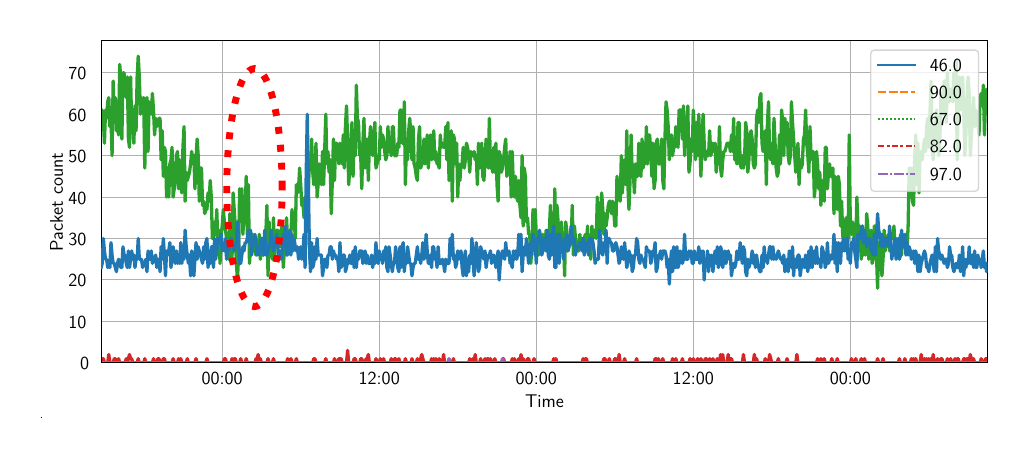
\begin{tikzpicture}
            \node(A){
            \resizebox{1\textwidth}{!}
            {
                %% Creator: Matplotlib, PGF backend
%%
%% To include the figure in your LaTeX document, write
%%   \input{<filename>.pgf}
%%
%% Make sure the required packages are loaded in your preamble
%%   \usepackage{pgf}
%%
%% Also ensure that all the required font packages are loaded; for instance,
%% the lmodern package is sometimes necessary when using math font.
%%   \usepackage{lmodern}
%%
%% Figures using additional raster images can only be included by \input if
%% they are in the same directory as the main LaTeX file. For loading figures
%% from other directories you can use the `import` package
%%   \usepackage{import}
%%
%% and then include the figures with
%%   \import{<path to file>}{<filename>.pgf}
%%
%% Matplotlib used the following preamble
%%   \usepackage{fontspec}
%%   \setmainfont{DejaVuSerif.ttf}[Path=\detokenize{/home/ankimme/fit/ibt/env/lib/python3.10/site-packages/matplotlib/mpl-data/fonts/ttf/}]
%%   \setsansfont{DejaVuSans.ttf}[Path=\detokenize{/home/ankimme/fit/ibt/env/lib/python3.10/site-packages/matplotlib/mpl-data/fonts/ttf/}]
%%   \setmonofont{DejaVuSansMono.ttf}[Path=\detokenize{/home/ankimme/fit/ibt/env/lib/python3.10/site-packages/matplotlib/mpl-data/fonts/ttf/}]
%%
\begingroup%
\makeatletter%
\begin{pgfpicture}%
\pgfpathrectangle{\pgfpointorigin}{\pgfqpoint{10.000000in}{4.000000in}}%
\pgfusepath{use as bounding box, clip}%
\begin{pgfscope}%
\pgfsetbuttcap%
\pgfsetmiterjoin%
\pgfsetlinewidth{0.000000pt}%
\definecolor{currentstroke}{rgb}{1.000000,1.000000,1.000000}%
\pgfsetstrokecolor{currentstroke}%
\pgfsetstrokeopacity{0.000000}%
\pgfsetdash{}{0pt}%
\pgfpathmoveto{\pgfqpoint{0.000000in}{0.000000in}}%
\pgfpathlineto{\pgfqpoint{10.000000in}{0.000000in}}%
\pgfpathlineto{\pgfqpoint{10.000000in}{4.000000in}}%
\pgfpathlineto{\pgfqpoint{0.000000in}{4.000000in}}%
\pgfpathlineto{\pgfqpoint{0.000000in}{0.000000in}}%
\pgfpathclose%
\pgfusepath{}%
\end{pgfscope}%
\begin{pgfscope}%
\pgfsetbuttcap%
\pgfsetmiterjoin%
\definecolor{currentfill}{rgb}{1.000000,1.000000,1.000000}%
\pgfsetfillcolor{currentfill}%
\pgfsetlinewidth{0.000000pt}%
\definecolor{currentstroke}{rgb}{0.000000,0.000000,0.000000}%
\pgfsetstrokecolor{currentstroke}%
\pgfsetstrokeopacity{0.000000}%
\pgfsetdash{}{0pt}%
\pgfpathmoveto{\pgfqpoint{0.630049in}{0.570804in}}%
\pgfpathlineto{\pgfqpoint{9.958330in}{0.570804in}}%
\pgfpathlineto{\pgfqpoint{9.958330in}{3.958330in}}%
\pgfpathlineto{\pgfqpoint{0.630049in}{3.958330in}}%
\pgfpathlineto{\pgfqpoint{0.630049in}{0.570804in}}%
\pgfpathclose%
\pgfusepath{fill}%
\end{pgfscope}%
\begin{pgfscope}%
\pgfpathrectangle{\pgfqpoint{0.630049in}{0.570804in}}{\pgfqpoint{9.328281in}{3.387526in}}%
\pgfusepath{clip}%
\pgfsetrectcap%
\pgfsetroundjoin%
\pgfsetlinewidth{0.803000pt}%
\definecolor{currentstroke}{rgb}{0.690196,0.690196,0.690196}%
\pgfsetstrokecolor{currentstroke}%
\pgfsetdash{}{0pt}%
\pgfpathmoveto{\pgfqpoint{1.903652in}{0.570804in}}%
\pgfpathlineto{\pgfqpoint{1.903652in}{3.958330in}}%
\pgfusepath{stroke}%
\end{pgfscope}%
\begin{pgfscope}%
\pgfsetbuttcap%
\pgfsetroundjoin%
\definecolor{currentfill}{rgb}{0.000000,0.000000,0.000000}%
\pgfsetfillcolor{currentfill}%
\pgfsetlinewidth{0.803000pt}%
\definecolor{currentstroke}{rgb}{0.000000,0.000000,0.000000}%
\pgfsetstrokecolor{currentstroke}%
\pgfsetdash{}{0pt}%
\pgfsys@defobject{currentmarker}{\pgfqpoint{0.000000in}{-0.048611in}}{\pgfqpoint{0.000000in}{0.000000in}}{%
\pgfpathmoveto{\pgfqpoint{0.000000in}{0.000000in}}%
\pgfpathlineto{\pgfqpoint{0.000000in}{-0.048611in}}%
\pgfusepath{stroke,fill}%
}%
\begin{pgfscope}%
\pgfsys@transformshift{1.903652in}{0.570804in}%
\pgfsys@useobject{currentmarker}{}%
\end{pgfscope}%
\end{pgfscope}%
\begin{pgfscope}%
\definecolor{textcolor}{rgb}{0.000000,0.000000,0.000000}%
\pgfsetstrokecolor{textcolor}%
\pgfsetfillcolor{textcolor}%
\pgftext[x=1.903652in,y=0.473582in,,top]{\color{textcolor}\sffamily\fontsize{14.000000}{16.800000}\selectfont 00:00}%
\end{pgfscope}%
\begin{pgfscope}%
\pgfpathrectangle{\pgfqpoint{0.630049in}{0.570804in}}{\pgfqpoint{9.328281in}{3.387526in}}%
\pgfusepath{clip}%
\pgfsetrectcap%
\pgfsetroundjoin%
\pgfsetlinewidth{0.803000pt}%
\definecolor{currentstroke}{rgb}{0.690196,0.690196,0.690196}%
\pgfsetstrokecolor{currentstroke}%
\pgfsetdash{}{0pt}%
\pgfpathmoveto{\pgfqpoint{3.555893in}{0.570804in}}%
\pgfpathlineto{\pgfqpoint{3.555893in}{3.958330in}}%
\pgfusepath{stroke}%
\end{pgfscope}%
\begin{pgfscope}%
\pgfsetbuttcap%
\pgfsetroundjoin%
\definecolor{currentfill}{rgb}{0.000000,0.000000,0.000000}%
\pgfsetfillcolor{currentfill}%
\pgfsetlinewidth{0.803000pt}%
\definecolor{currentstroke}{rgb}{0.000000,0.000000,0.000000}%
\pgfsetstrokecolor{currentstroke}%
\pgfsetdash{}{0pt}%
\pgfsys@defobject{currentmarker}{\pgfqpoint{0.000000in}{-0.048611in}}{\pgfqpoint{0.000000in}{0.000000in}}{%
\pgfpathmoveto{\pgfqpoint{0.000000in}{0.000000in}}%
\pgfpathlineto{\pgfqpoint{0.000000in}{-0.048611in}}%
\pgfusepath{stroke,fill}%
}%
\begin{pgfscope}%
\pgfsys@transformshift{3.555893in}{0.570804in}%
\pgfsys@useobject{currentmarker}{}%
\end{pgfscope}%
\end{pgfscope}%
\begin{pgfscope}%
\definecolor{textcolor}{rgb}{0.000000,0.000000,0.000000}%
\pgfsetstrokecolor{textcolor}%
\pgfsetfillcolor{textcolor}%
\pgftext[x=3.555893in,y=0.473582in,,top]{\color{textcolor}\sffamily\fontsize{14.000000}{16.800000}\selectfont 12:00}%
\end{pgfscope}%
\begin{pgfscope}%
\pgfpathrectangle{\pgfqpoint{0.630049in}{0.570804in}}{\pgfqpoint{9.328281in}{3.387526in}}%
\pgfusepath{clip}%
\pgfsetrectcap%
\pgfsetroundjoin%
\pgfsetlinewidth{0.803000pt}%
\definecolor{currentstroke}{rgb}{0.690196,0.690196,0.690196}%
\pgfsetstrokecolor{currentstroke}%
\pgfsetdash{}{0pt}%
\pgfpathmoveto{\pgfqpoint{5.208135in}{0.570804in}}%
\pgfpathlineto{\pgfqpoint{5.208135in}{3.958330in}}%
\pgfusepath{stroke}%
\end{pgfscope}%
\begin{pgfscope}%
\pgfsetbuttcap%
\pgfsetroundjoin%
\definecolor{currentfill}{rgb}{0.000000,0.000000,0.000000}%
\pgfsetfillcolor{currentfill}%
\pgfsetlinewidth{0.803000pt}%
\definecolor{currentstroke}{rgb}{0.000000,0.000000,0.000000}%
\pgfsetstrokecolor{currentstroke}%
\pgfsetdash{}{0pt}%
\pgfsys@defobject{currentmarker}{\pgfqpoint{0.000000in}{-0.048611in}}{\pgfqpoint{0.000000in}{0.000000in}}{%
\pgfpathmoveto{\pgfqpoint{0.000000in}{0.000000in}}%
\pgfpathlineto{\pgfqpoint{0.000000in}{-0.048611in}}%
\pgfusepath{stroke,fill}%
}%
\begin{pgfscope}%
\pgfsys@transformshift{5.208135in}{0.570804in}%
\pgfsys@useobject{currentmarker}{}%
\end{pgfscope}%
\end{pgfscope}%
\begin{pgfscope}%
\definecolor{textcolor}{rgb}{0.000000,0.000000,0.000000}%
\pgfsetstrokecolor{textcolor}%
\pgfsetfillcolor{textcolor}%
\pgftext[x=5.208135in,y=0.473582in,,top]{\color{textcolor}\sffamily\fontsize{14.000000}{16.800000}\selectfont 00:00}%
\end{pgfscope}%
\begin{pgfscope}%
\pgfpathrectangle{\pgfqpoint{0.630049in}{0.570804in}}{\pgfqpoint{9.328281in}{3.387526in}}%
\pgfusepath{clip}%
\pgfsetrectcap%
\pgfsetroundjoin%
\pgfsetlinewidth{0.803000pt}%
\definecolor{currentstroke}{rgb}{0.690196,0.690196,0.690196}%
\pgfsetstrokecolor{currentstroke}%
\pgfsetdash{}{0pt}%
\pgfpathmoveto{\pgfqpoint{6.860377in}{0.570804in}}%
\pgfpathlineto{\pgfqpoint{6.860377in}{3.958330in}}%
\pgfusepath{stroke}%
\end{pgfscope}%
\begin{pgfscope}%
\pgfsetbuttcap%
\pgfsetroundjoin%
\definecolor{currentfill}{rgb}{0.000000,0.000000,0.000000}%
\pgfsetfillcolor{currentfill}%
\pgfsetlinewidth{0.803000pt}%
\definecolor{currentstroke}{rgb}{0.000000,0.000000,0.000000}%
\pgfsetstrokecolor{currentstroke}%
\pgfsetdash{}{0pt}%
\pgfsys@defobject{currentmarker}{\pgfqpoint{0.000000in}{-0.048611in}}{\pgfqpoint{0.000000in}{0.000000in}}{%
\pgfpathmoveto{\pgfqpoint{0.000000in}{0.000000in}}%
\pgfpathlineto{\pgfqpoint{0.000000in}{-0.048611in}}%
\pgfusepath{stroke,fill}%
}%
\begin{pgfscope}%
\pgfsys@transformshift{6.860377in}{0.570804in}%
\pgfsys@useobject{currentmarker}{}%
\end{pgfscope}%
\end{pgfscope}%
\begin{pgfscope}%
\definecolor{textcolor}{rgb}{0.000000,0.000000,0.000000}%
\pgfsetstrokecolor{textcolor}%
\pgfsetfillcolor{textcolor}%
\pgftext[x=6.860377in,y=0.473582in,,top]{\color{textcolor}\sffamily\fontsize{14.000000}{16.800000}\selectfont 12:00}%
\end{pgfscope}%
\begin{pgfscope}%
\pgfpathrectangle{\pgfqpoint{0.630049in}{0.570804in}}{\pgfqpoint{9.328281in}{3.387526in}}%
\pgfusepath{clip}%
\pgfsetrectcap%
\pgfsetroundjoin%
\pgfsetlinewidth{0.803000pt}%
\definecolor{currentstroke}{rgb}{0.690196,0.690196,0.690196}%
\pgfsetstrokecolor{currentstroke}%
\pgfsetdash{}{0pt}%
\pgfpathmoveto{\pgfqpoint{8.512619in}{0.570804in}}%
\pgfpathlineto{\pgfqpoint{8.512619in}{3.958330in}}%
\pgfusepath{stroke}%
\end{pgfscope}%
\begin{pgfscope}%
\pgfsetbuttcap%
\pgfsetroundjoin%
\definecolor{currentfill}{rgb}{0.000000,0.000000,0.000000}%
\pgfsetfillcolor{currentfill}%
\pgfsetlinewidth{0.803000pt}%
\definecolor{currentstroke}{rgb}{0.000000,0.000000,0.000000}%
\pgfsetstrokecolor{currentstroke}%
\pgfsetdash{}{0pt}%
\pgfsys@defobject{currentmarker}{\pgfqpoint{0.000000in}{-0.048611in}}{\pgfqpoint{0.000000in}{0.000000in}}{%
\pgfpathmoveto{\pgfqpoint{0.000000in}{0.000000in}}%
\pgfpathlineto{\pgfqpoint{0.000000in}{-0.048611in}}%
\pgfusepath{stroke,fill}%
}%
\begin{pgfscope}%
\pgfsys@transformshift{8.512619in}{0.570804in}%
\pgfsys@useobject{currentmarker}{}%
\end{pgfscope}%
\end{pgfscope}%
\begin{pgfscope}%
\definecolor{textcolor}{rgb}{0.000000,0.000000,0.000000}%
\pgfsetstrokecolor{textcolor}%
\pgfsetfillcolor{textcolor}%
\pgftext[x=8.512619in,y=0.473582in,,top]{\color{textcolor}\sffamily\fontsize{14.000000}{16.800000}\selectfont 00:00}%
\end{pgfscope}%
\begin{pgfscope}%
\definecolor{textcolor}{rgb}{0.000000,0.000000,0.000000}%
\pgfsetstrokecolor{textcolor}%
\pgfsetfillcolor{textcolor}%
\pgftext[x=5.294189in,y=0.229848in,,top]{\color{textcolor}\sffamily\fontsize{14.000000}{16.800000}\selectfont Time}%
\end{pgfscope}%
\begin{pgfscope}%
\pgfpathrectangle{\pgfqpoint{0.630049in}{0.570804in}}{\pgfqpoint{9.328281in}{3.387526in}}%
\pgfusepath{clip}%
\pgfsetrectcap%
\pgfsetroundjoin%
\pgfsetlinewidth{0.803000pt}%
\definecolor{currentstroke}{rgb}{0.690196,0.690196,0.690196}%
\pgfsetstrokecolor{currentstroke}%
\pgfsetdash{}{0pt}%
\pgfpathmoveto{\pgfqpoint{0.630049in}{0.570804in}}%
\pgfpathlineto{\pgfqpoint{9.958330in}{0.570804in}}%
\pgfusepath{stroke}%
\end{pgfscope}%
\begin{pgfscope}%
\pgfsetbuttcap%
\pgfsetroundjoin%
\definecolor{currentfill}{rgb}{0.000000,0.000000,0.000000}%
\pgfsetfillcolor{currentfill}%
\pgfsetlinewidth{0.803000pt}%
\definecolor{currentstroke}{rgb}{0.000000,0.000000,0.000000}%
\pgfsetstrokecolor{currentstroke}%
\pgfsetdash{}{0pt}%
\pgfsys@defobject{currentmarker}{\pgfqpoint{-0.048611in}{0.000000in}}{\pgfqpoint{-0.000000in}{0.000000in}}{%
\pgfpathmoveto{\pgfqpoint{-0.000000in}{0.000000in}}%
\pgfpathlineto{\pgfqpoint{-0.048611in}{0.000000in}}%
\pgfusepath{stroke,fill}%
}%
\begin{pgfscope}%
\pgfsys@transformshift{0.630049in}{0.570804in}%
\pgfsys@useobject{currentmarker}{}%
\end{pgfscope}%
\end{pgfscope}%
\begin{pgfscope}%
\definecolor{textcolor}{rgb}{0.000000,0.000000,0.000000}%
\pgfsetstrokecolor{textcolor}%
\pgfsetfillcolor{textcolor}%
\pgftext[x=0.409115in, y=0.496938in, left, base]{\color{textcolor}\sffamily\fontsize{14.000000}{16.800000}\selectfont 0}%
\end{pgfscope}%
\begin{pgfscope}%
\pgfpathrectangle{\pgfqpoint{0.630049in}{0.570804in}}{\pgfqpoint{9.328281in}{3.387526in}}%
\pgfusepath{clip}%
\pgfsetrectcap%
\pgfsetroundjoin%
\pgfsetlinewidth{0.803000pt}%
\definecolor{currentstroke}{rgb}{0.690196,0.690196,0.690196}%
\pgfsetstrokecolor{currentstroke}%
\pgfsetdash{}{0pt}%
\pgfpathmoveto{\pgfqpoint{0.630049in}{1.006779in}}%
\pgfpathlineto{\pgfqpoint{9.958330in}{1.006779in}}%
\pgfusepath{stroke}%
\end{pgfscope}%
\begin{pgfscope}%
\pgfsetbuttcap%
\pgfsetroundjoin%
\definecolor{currentfill}{rgb}{0.000000,0.000000,0.000000}%
\pgfsetfillcolor{currentfill}%
\pgfsetlinewidth{0.803000pt}%
\definecolor{currentstroke}{rgb}{0.000000,0.000000,0.000000}%
\pgfsetstrokecolor{currentstroke}%
\pgfsetdash{}{0pt}%
\pgfsys@defobject{currentmarker}{\pgfqpoint{-0.048611in}{0.000000in}}{\pgfqpoint{-0.000000in}{0.000000in}}{%
\pgfpathmoveto{\pgfqpoint{-0.000000in}{0.000000in}}%
\pgfpathlineto{\pgfqpoint{-0.048611in}{0.000000in}}%
\pgfusepath{stroke,fill}%
}%
\begin{pgfscope}%
\pgfsys@transformshift{0.630049in}{1.006779in}%
\pgfsys@useobject{currentmarker}{}%
\end{pgfscope}%
\end{pgfscope}%
\begin{pgfscope}%
\definecolor{textcolor}{rgb}{0.000000,0.000000,0.000000}%
\pgfsetstrokecolor{textcolor}%
\pgfsetfillcolor{textcolor}%
\pgftext[x=0.285404in, y=0.932913in, left, base]{\color{textcolor}\sffamily\fontsize{14.000000}{16.800000}\selectfont 10}%
\end{pgfscope}%
\begin{pgfscope}%
\pgfpathrectangle{\pgfqpoint{0.630049in}{0.570804in}}{\pgfqpoint{9.328281in}{3.387526in}}%
\pgfusepath{clip}%
\pgfsetrectcap%
\pgfsetroundjoin%
\pgfsetlinewidth{0.803000pt}%
\definecolor{currentstroke}{rgb}{0.690196,0.690196,0.690196}%
\pgfsetstrokecolor{currentstroke}%
\pgfsetdash{}{0pt}%
\pgfpathmoveto{\pgfqpoint{0.630049in}{1.442754in}}%
\pgfpathlineto{\pgfqpoint{9.958330in}{1.442754in}}%
\pgfusepath{stroke}%
\end{pgfscope}%
\begin{pgfscope}%
\pgfsetbuttcap%
\pgfsetroundjoin%
\definecolor{currentfill}{rgb}{0.000000,0.000000,0.000000}%
\pgfsetfillcolor{currentfill}%
\pgfsetlinewidth{0.803000pt}%
\definecolor{currentstroke}{rgb}{0.000000,0.000000,0.000000}%
\pgfsetstrokecolor{currentstroke}%
\pgfsetdash{}{0pt}%
\pgfsys@defobject{currentmarker}{\pgfqpoint{-0.048611in}{0.000000in}}{\pgfqpoint{-0.000000in}{0.000000in}}{%
\pgfpathmoveto{\pgfqpoint{-0.000000in}{0.000000in}}%
\pgfpathlineto{\pgfqpoint{-0.048611in}{0.000000in}}%
\pgfusepath{stroke,fill}%
}%
\begin{pgfscope}%
\pgfsys@transformshift{0.630049in}{1.442754in}%
\pgfsys@useobject{currentmarker}{}%
\end{pgfscope}%
\end{pgfscope}%
\begin{pgfscope}%
\definecolor{textcolor}{rgb}{0.000000,0.000000,0.000000}%
\pgfsetstrokecolor{textcolor}%
\pgfsetfillcolor{textcolor}%
\pgftext[x=0.285404in, y=1.368888in, left, base]{\color{textcolor}\sffamily\fontsize{14.000000}{16.800000}\selectfont 20}%
\end{pgfscope}%
\begin{pgfscope}%
\pgfpathrectangle{\pgfqpoint{0.630049in}{0.570804in}}{\pgfqpoint{9.328281in}{3.387526in}}%
\pgfusepath{clip}%
\pgfsetrectcap%
\pgfsetroundjoin%
\pgfsetlinewidth{0.803000pt}%
\definecolor{currentstroke}{rgb}{0.690196,0.690196,0.690196}%
\pgfsetstrokecolor{currentstroke}%
\pgfsetdash{}{0pt}%
\pgfpathmoveto{\pgfqpoint{0.630049in}{1.878729in}}%
\pgfpathlineto{\pgfqpoint{9.958330in}{1.878729in}}%
\pgfusepath{stroke}%
\end{pgfscope}%
\begin{pgfscope}%
\pgfsetbuttcap%
\pgfsetroundjoin%
\definecolor{currentfill}{rgb}{0.000000,0.000000,0.000000}%
\pgfsetfillcolor{currentfill}%
\pgfsetlinewidth{0.803000pt}%
\definecolor{currentstroke}{rgb}{0.000000,0.000000,0.000000}%
\pgfsetstrokecolor{currentstroke}%
\pgfsetdash{}{0pt}%
\pgfsys@defobject{currentmarker}{\pgfqpoint{-0.048611in}{0.000000in}}{\pgfqpoint{-0.000000in}{0.000000in}}{%
\pgfpathmoveto{\pgfqpoint{-0.000000in}{0.000000in}}%
\pgfpathlineto{\pgfqpoint{-0.048611in}{0.000000in}}%
\pgfusepath{stroke,fill}%
}%
\begin{pgfscope}%
\pgfsys@transformshift{0.630049in}{1.878729in}%
\pgfsys@useobject{currentmarker}{}%
\end{pgfscope}%
\end{pgfscope}%
\begin{pgfscope}%
\definecolor{textcolor}{rgb}{0.000000,0.000000,0.000000}%
\pgfsetstrokecolor{textcolor}%
\pgfsetfillcolor{textcolor}%
\pgftext[x=0.285404in, y=1.804863in, left, base]{\color{textcolor}\sffamily\fontsize{14.000000}{16.800000}\selectfont 30}%
\end{pgfscope}%
\begin{pgfscope}%
\pgfpathrectangle{\pgfqpoint{0.630049in}{0.570804in}}{\pgfqpoint{9.328281in}{3.387526in}}%
\pgfusepath{clip}%
\pgfsetrectcap%
\pgfsetroundjoin%
\pgfsetlinewidth{0.803000pt}%
\definecolor{currentstroke}{rgb}{0.690196,0.690196,0.690196}%
\pgfsetstrokecolor{currentstroke}%
\pgfsetdash{}{0pt}%
\pgfpathmoveto{\pgfqpoint{0.630049in}{2.314704in}}%
\pgfpathlineto{\pgfqpoint{9.958330in}{2.314704in}}%
\pgfusepath{stroke}%
\end{pgfscope}%
\begin{pgfscope}%
\pgfsetbuttcap%
\pgfsetroundjoin%
\definecolor{currentfill}{rgb}{0.000000,0.000000,0.000000}%
\pgfsetfillcolor{currentfill}%
\pgfsetlinewidth{0.803000pt}%
\definecolor{currentstroke}{rgb}{0.000000,0.000000,0.000000}%
\pgfsetstrokecolor{currentstroke}%
\pgfsetdash{}{0pt}%
\pgfsys@defobject{currentmarker}{\pgfqpoint{-0.048611in}{0.000000in}}{\pgfqpoint{-0.000000in}{0.000000in}}{%
\pgfpathmoveto{\pgfqpoint{-0.000000in}{0.000000in}}%
\pgfpathlineto{\pgfqpoint{-0.048611in}{0.000000in}}%
\pgfusepath{stroke,fill}%
}%
\begin{pgfscope}%
\pgfsys@transformshift{0.630049in}{2.314704in}%
\pgfsys@useobject{currentmarker}{}%
\end{pgfscope}%
\end{pgfscope}%
\begin{pgfscope}%
\definecolor{textcolor}{rgb}{0.000000,0.000000,0.000000}%
\pgfsetstrokecolor{textcolor}%
\pgfsetfillcolor{textcolor}%
\pgftext[x=0.285404in, y=2.240838in, left, base]{\color{textcolor}\sffamily\fontsize{14.000000}{16.800000}\selectfont 40}%
\end{pgfscope}%
\begin{pgfscope}%
\pgfpathrectangle{\pgfqpoint{0.630049in}{0.570804in}}{\pgfqpoint{9.328281in}{3.387526in}}%
\pgfusepath{clip}%
\pgfsetrectcap%
\pgfsetroundjoin%
\pgfsetlinewidth{0.803000pt}%
\definecolor{currentstroke}{rgb}{0.690196,0.690196,0.690196}%
\pgfsetstrokecolor{currentstroke}%
\pgfsetdash{}{0pt}%
\pgfpathmoveto{\pgfqpoint{0.630049in}{2.750679in}}%
\pgfpathlineto{\pgfqpoint{9.958330in}{2.750679in}}%
\pgfusepath{stroke}%
\end{pgfscope}%
\begin{pgfscope}%
\pgfsetbuttcap%
\pgfsetroundjoin%
\definecolor{currentfill}{rgb}{0.000000,0.000000,0.000000}%
\pgfsetfillcolor{currentfill}%
\pgfsetlinewidth{0.803000pt}%
\definecolor{currentstroke}{rgb}{0.000000,0.000000,0.000000}%
\pgfsetstrokecolor{currentstroke}%
\pgfsetdash{}{0pt}%
\pgfsys@defobject{currentmarker}{\pgfqpoint{-0.048611in}{0.000000in}}{\pgfqpoint{-0.000000in}{0.000000in}}{%
\pgfpathmoveto{\pgfqpoint{-0.000000in}{0.000000in}}%
\pgfpathlineto{\pgfqpoint{-0.048611in}{0.000000in}}%
\pgfusepath{stroke,fill}%
}%
\begin{pgfscope}%
\pgfsys@transformshift{0.630049in}{2.750679in}%
\pgfsys@useobject{currentmarker}{}%
\end{pgfscope}%
\end{pgfscope}%
\begin{pgfscope}%
\definecolor{textcolor}{rgb}{0.000000,0.000000,0.000000}%
\pgfsetstrokecolor{textcolor}%
\pgfsetfillcolor{textcolor}%
\pgftext[x=0.285404in, y=2.676813in, left, base]{\color{textcolor}\sffamily\fontsize{14.000000}{16.800000}\selectfont 50}%
\end{pgfscope}%
\begin{pgfscope}%
\pgfpathrectangle{\pgfqpoint{0.630049in}{0.570804in}}{\pgfqpoint{9.328281in}{3.387526in}}%
\pgfusepath{clip}%
\pgfsetrectcap%
\pgfsetroundjoin%
\pgfsetlinewidth{0.803000pt}%
\definecolor{currentstroke}{rgb}{0.690196,0.690196,0.690196}%
\pgfsetstrokecolor{currentstroke}%
\pgfsetdash{}{0pt}%
\pgfpathmoveto{\pgfqpoint{0.630049in}{3.186654in}}%
\pgfpathlineto{\pgfqpoint{9.958330in}{3.186654in}}%
\pgfusepath{stroke}%
\end{pgfscope}%
\begin{pgfscope}%
\pgfsetbuttcap%
\pgfsetroundjoin%
\definecolor{currentfill}{rgb}{0.000000,0.000000,0.000000}%
\pgfsetfillcolor{currentfill}%
\pgfsetlinewidth{0.803000pt}%
\definecolor{currentstroke}{rgb}{0.000000,0.000000,0.000000}%
\pgfsetstrokecolor{currentstroke}%
\pgfsetdash{}{0pt}%
\pgfsys@defobject{currentmarker}{\pgfqpoint{-0.048611in}{0.000000in}}{\pgfqpoint{-0.000000in}{0.000000in}}{%
\pgfpathmoveto{\pgfqpoint{-0.000000in}{0.000000in}}%
\pgfpathlineto{\pgfqpoint{-0.048611in}{0.000000in}}%
\pgfusepath{stroke,fill}%
}%
\begin{pgfscope}%
\pgfsys@transformshift{0.630049in}{3.186654in}%
\pgfsys@useobject{currentmarker}{}%
\end{pgfscope}%
\end{pgfscope}%
\begin{pgfscope}%
\definecolor{textcolor}{rgb}{0.000000,0.000000,0.000000}%
\pgfsetstrokecolor{textcolor}%
\pgfsetfillcolor{textcolor}%
\pgftext[x=0.285404in, y=3.112788in, left, base]{\color{textcolor}\sffamily\fontsize{14.000000}{16.800000}\selectfont 60}%
\end{pgfscope}%
\begin{pgfscope}%
\pgfpathrectangle{\pgfqpoint{0.630049in}{0.570804in}}{\pgfqpoint{9.328281in}{3.387526in}}%
\pgfusepath{clip}%
\pgfsetrectcap%
\pgfsetroundjoin%
\pgfsetlinewidth{0.803000pt}%
\definecolor{currentstroke}{rgb}{0.690196,0.690196,0.690196}%
\pgfsetstrokecolor{currentstroke}%
\pgfsetdash{}{0pt}%
\pgfpathmoveto{\pgfqpoint{0.630049in}{3.622629in}}%
\pgfpathlineto{\pgfqpoint{9.958330in}{3.622629in}}%
\pgfusepath{stroke}%
\end{pgfscope}%
\begin{pgfscope}%
\pgfsetbuttcap%
\pgfsetroundjoin%
\definecolor{currentfill}{rgb}{0.000000,0.000000,0.000000}%
\pgfsetfillcolor{currentfill}%
\pgfsetlinewidth{0.803000pt}%
\definecolor{currentstroke}{rgb}{0.000000,0.000000,0.000000}%
\pgfsetstrokecolor{currentstroke}%
\pgfsetdash{}{0pt}%
\pgfsys@defobject{currentmarker}{\pgfqpoint{-0.048611in}{0.000000in}}{\pgfqpoint{-0.000000in}{0.000000in}}{%
\pgfpathmoveto{\pgfqpoint{-0.000000in}{0.000000in}}%
\pgfpathlineto{\pgfqpoint{-0.048611in}{0.000000in}}%
\pgfusepath{stroke,fill}%
}%
\begin{pgfscope}%
\pgfsys@transformshift{0.630049in}{3.622629in}%
\pgfsys@useobject{currentmarker}{}%
\end{pgfscope}%
\end{pgfscope}%
\begin{pgfscope}%
\definecolor{textcolor}{rgb}{0.000000,0.000000,0.000000}%
\pgfsetstrokecolor{textcolor}%
\pgfsetfillcolor{textcolor}%
\pgftext[x=0.285404in, y=3.548763in, left, base]{\color{textcolor}\sffamily\fontsize{14.000000}{16.800000}\selectfont 70}%
\end{pgfscope}%
\begin{pgfscope}%
\definecolor{textcolor}{rgb}{0.000000,0.000000,0.000000}%
\pgfsetstrokecolor{textcolor}%
\pgfsetfillcolor{textcolor}%
\pgftext[x=0.229848in,y=2.264567in,,bottom,rotate=90.000000]{\color{textcolor}\sffamily\fontsize{14.000000}{16.800000}\selectfont Packet count}%
\end{pgfscope}%
\begin{pgfscope}%
\pgfpathrectangle{\pgfqpoint{0.630049in}{0.570804in}}{\pgfqpoint{9.328281in}{3.387526in}}%
\pgfusepath{clip}%
\pgfsetrectcap%
\pgfsetroundjoin%
\pgfsetlinewidth{2.509375pt}%
\definecolor{currentstroke}{rgb}{1.000000,0.498039,0.054902}%
\pgfsetstrokecolor{currentstroke}%
\pgfsetdash{}{0pt}%
\pgfpathmoveto{\pgfqpoint{0.630049in}{0.570804in}}%
\pgfpathlineto{\pgfqpoint{9.958330in}{0.570804in}}%
\pgfpathlineto{\pgfqpoint{9.958330in}{0.570804in}}%
\pgfusepath{stroke}%
\end{pgfscope}%
\begin{pgfscope}%
\pgfpathrectangle{\pgfqpoint{0.630049in}{0.570804in}}{\pgfqpoint{9.328281in}{3.387526in}}%
\pgfusepath{clip}%
\pgfsetrectcap%
\pgfsetroundjoin%
\pgfsetlinewidth{2.509375pt}%
\definecolor{currentstroke}{rgb}{0.172549,0.627451,0.172549}%
\pgfsetstrokecolor{currentstroke}%
\pgfsetdash{}{0pt}%
\pgfpathmoveto{\pgfqpoint{0.630049in}{3.230252in}}%
\pgfpathlineto{\pgfqpoint{0.641523in}{3.230252in}}%
\pgfpathlineto{\pgfqpoint{0.652997in}{3.143057in}}%
\pgfpathlineto{\pgfqpoint{0.664470in}{2.881472in}}%
\pgfpathlineto{\pgfqpoint{0.675944in}{3.230252in}}%
\pgfpathlineto{\pgfqpoint{0.687418in}{3.143057in}}%
\pgfpathlineto{\pgfqpoint{0.698892in}{3.317447in}}%
\pgfpathlineto{\pgfqpoint{0.710366in}{3.361044in}}%
\pgfpathlineto{\pgfqpoint{0.721840in}{3.055862in}}%
\pgfpathlineto{\pgfqpoint{0.733314in}{3.143057in}}%
\pgfpathlineto{\pgfqpoint{0.744788in}{2.750679in}}%
\pgfpathlineto{\pgfqpoint{0.756262in}{3.535434in}}%
\pgfpathlineto{\pgfqpoint{0.767736in}{3.099459in}}%
\pgfpathlineto{\pgfqpoint{0.779209in}{3.361044in}}%
\pgfpathlineto{\pgfqpoint{0.790683in}{3.012264in}}%
\pgfpathlineto{\pgfqpoint{0.802157in}{3.055862in}}%
\pgfpathlineto{\pgfqpoint{0.813631in}{2.968667in}}%
\pgfpathlineto{\pgfqpoint{0.825105in}{3.709824in}}%
\pgfpathlineto{\pgfqpoint{0.836579in}{3.579032in}}%
\pgfpathlineto{\pgfqpoint{0.848053in}{2.925069in}}%
\pgfpathlineto{\pgfqpoint{0.859527in}{3.622629in}}%
\pgfpathlineto{\pgfqpoint{0.871001in}{3.622629in}}%
\pgfpathlineto{\pgfqpoint{0.882475in}{3.448239in}}%
\pgfpathlineto{\pgfqpoint{0.893948in}{3.361044in}}%
\pgfpathlineto{\pgfqpoint{0.905422in}{3.579032in}}%
\pgfpathlineto{\pgfqpoint{0.916896in}{2.925069in}}%
\pgfpathlineto{\pgfqpoint{0.928370in}{2.837874in}}%
\pgfpathlineto{\pgfqpoint{0.939844in}{3.579032in}}%
\pgfpathlineto{\pgfqpoint{0.951318in}{3.055862in}}%
\pgfpathlineto{\pgfqpoint{0.962792in}{3.099459in}}%
\pgfpathlineto{\pgfqpoint{0.974266in}{2.881472in}}%
\pgfpathlineto{\pgfqpoint{0.985740in}{3.273849in}}%
\pgfpathlineto{\pgfqpoint{0.997214in}{3.012264in}}%
\pgfpathlineto{\pgfqpoint{1.008687in}{3.579032in}}%
\pgfpathlineto{\pgfqpoint{1.020161in}{3.797019in}}%
\pgfpathlineto{\pgfqpoint{1.031635in}{3.579032in}}%
\pgfpathlineto{\pgfqpoint{1.043109in}{3.186654in}}%
\pgfpathlineto{\pgfqpoint{1.054583in}{3.361044in}}%
\pgfpathlineto{\pgfqpoint{1.066057in}{3.317447in}}%
\pgfpathlineto{\pgfqpoint{1.077531in}{3.361044in}}%
\pgfpathlineto{\pgfqpoint{1.089005in}{2.619887in}}%
\pgfpathlineto{\pgfqpoint{1.100479in}{3.143057in}}%
\pgfpathlineto{\pgfqpoint{1.111953in}{3.361044in}}%
\pgfpathlineto{\pgfqpoint{1.123426in}{2.794277in}}%
\pgfpathlineto{\pgfqpoint{1.134900in}{3.317447in}}%
\pgfpathlineto{\pgfqpoint{1.146374in}{3.273849in}}%
\pgfpathlineto{\pgfqpoint{1.157848in}{3.186654in}}%
\pgfpathlineto{\pgfqpoint{1.169322in}{3.404642in}}%
\pgfpathlineto{\pgfqpoint{1.180796in}{3.230252in}}%
\pgfpathlineto{\pgfqpoint{1.192270in}{2.968667in}}%
\pgfpathlineto{\pgfqpoint{1.203744in}{3.143057in}}%
\pgfpathlineto{\pgfqpoint{1.215218in}{3.055862in}}%
\pgfpathlineto{\pgfqpoint{1.238165in}{3.143057in}}%
\pgfpathlineto{\pgfqpoint{1.249639in}{3.143057in}}%
\pgfpathlineto{\pgfqpoint{1.261113in}{2.707082in}}%
\pgfpathlineto{\pgfqpoint{1.272587in}{3.012264in}}%
\pgfpathlineto{\pgfqpoint{1.284061in}{2.532692in}}%
\pgfpathlineto{\pgfqpoint{1.295535in}{2.837874in}}%
\pgfpathlineto{\pgfqpoint{1.307009in}{2.794277in}}%
\pgfpathlineto{\pgfqpoint{1.318483in}{2.314704in}}%
\pgfpathlineto{\pgfqpoint{1.329957in}{2.619887in}}%
\pgfpathlineto{\pgfqpoint{1.341431in}{2.314704in}}%
\pgfpathlineto{\pgfqpoint{1.352904in}{2.663484in}}%
\pgfpathlineto{\pgfqpoint{1.364378in}{2.707082in}}%
\pgfpathlineto{\pgfqpoint{1.375852in}{2.837874in}}%
\pgfpathlineto{\pgfqpoint{1.387326in}{2.314704in}}%
\pgfpathlineto{\pgfqpoint{1.410274in}{2.489094in}}%
\pgfpathlineto{\pgfqpoint{1.421748in}{2.750679in}}%
\pgfpathlineto{\pgfqpoint{1.433222in}{2.794277in}}%
\pgfpathlineto{\pgfqpoint{1.444696in}{2.401899in}}%
\pgfpathlineto{\pgfqpoint{1.456170in}{2.707082in}}%
\pgfpathlineto{\pgfqpoint{1.467643in}{2.445497in}}%
\pgfpathlineto{\pgfqpoint{1.479117in}{2.358302in}}%
\pgfpathlineto{\pgfqpoint{1.490591in}{2.837874in}}%
\pgfpathlineto{\pgfqpoint{1.502065in}{3.055862in}}%
\pgfpathlineto{\pgfqpoint{1.513539in}{2.271107in}}%
\pgfpathlineto{\pgfqpoint{1.525013in}{2.576289in}}%
\pgfpathlineto{\pgfqpoint{1.536487in}{2.489094in}}%
\pgfpathlineto{\pgfqpoint{1.559435in}{2.576289in}}%
\pgfpathlineto{\pgfqpoint{1.570909in}{2.663484in}}%
\pgfpathlineto{\pgfqpoint{1.582383in}{2.794277in}}%
\pgfpathlineto{\pgfqpoint{1.593856in}{2.707082in}}%
\pgfpathlineto{\pgfqpoint{1.605330in}{2.750679in}}%
\pgfpathlineto{\pgfqpoint{1.616804in}{2.401899in}}%
\pgfpathlineto{\pgfqpoint{1.628278in}{2.707082in}}%
\pgfpathlineto{\pgfqpoint{1.639752in}{2.925069in}}%
\pgfpathlineto{\pgfqpoint{1.651226in}{2.750679in}}%
\pgfpathlineto{\pgfqpoint{1.662700in}{2.271107in}}%
\pgfpathlineto{\pgfqpoint{1.674174in}{2.619887in}}%
\pgfpathlineto{\pgfqpoint{1.685648in}{2.619887in}}%
\pgfpathlineto{\pgfqpoint{1.697122in}{2.227509in}}%
\pgfpathlineto{\pgfqpoint{1.708595in}{2.271107in}}%
\pgfpathlineto{\pgfqpoint{1.720069in}{2.140314in}}%
\pgfpathlineto{\pgfqpoint{1.731543in}{2.183912in}}%
\pgfpathlineto{\pgfqpoint{1.743017in}{2.183912in}}%
\pgfpathlineto{\pgfqpoint{1.754491in}{2.358302in}}%
\pgfpathlineto{\pgfqpoint{1.765965in}{2.271107in}}%
\pgfpathlineto{\pgfqpoint{1.777439in}{2.489094in}}%
\pgfpathlineto{\pgfqpoint{1.788913in}{2.314704in}}%
\pgfpathlineto{\pgfqpoint{1.800387in}{1.878729in}}%
\pgfpathlineto{\pgfqpoint{1.811861in}{1.878729in}}%
\pgfpathlineto{\pgfqpoint{1.823334in}{2.053119in}}%
\pgfpathlineto{\pgfqpoint{1.834808in}{1.922327in}}%
\pgfpathlineto{\pgfqpoint{1.846282in}{2.183912in}}%
\pgfpathlineto{\pgfqpoint{1.857756in}{1.835132in}}%
\pgfpathlineto{\pgfqpoint{1.869230in}{1.965924in}}%
\pgfpathlineto{\pgfqpoint{1.880704in}{1.617144in}}%
\pgfpathlineto{\pgfqpoint{1.892178in}{1.922327in}}%
\pgfpathlineto{\pgfqpoint{1.903652in}{2.009522in}}%
\pgfpathlineto{\pgfqpoint{1.915126in}{2.183912in}}%
\pgfpathlineto{\pgfqpoint{1.926600in}{2.053119in}}%
\pgfpathlineto{\pgfqpoint{1.949547in}{1.878729in}}%
\pgfpathlineto{\pgfqpoint{1.961021in}{1.835132in}}%
\pgfpathlineto{\pgfqpoint{1.972495in}{1.660742in}}%
\pgfpathlineto{\pgfqpoint{1.983969in}{2.140314in}}%
\pgfpathlineto{\pgfqpoint{1.995443in}{1.835132in}}%
\pgfpathlineto{\pgfqpoint{2.006917in}{1.660742in}}%
\pgfpathlineto{\pgfqpoint{2.018391in}{2.358302in}}%
\pgfpathlineto{\pgfqpoint{2.041339in}{2.009522in}}%
\pgfpathlineto{\pgfqpoint{2.052812in}{1.617144in}}%
\pgfpathlineto{\pgfqpoint{2.064286in}{1.442754in}}%
\pgfpathlineto{\pgfqpoint{2.075760in}{1.704339in}}%
\pgfpathlineto{\pgfqpoint{2.087234in}{2.401899in}}%
\pgfpathlineto{\pgfqpoint{2.098708in}{2.358302in}}%
\pgfpathlineto{\pgfqpoint{2.110182in}{2.401899in}}%
\pgfpathlineto{\pgfqpoint{2.121656in}{1.922327in}}%
\pgfpathlineto{\pgfqpoint{2.133130in}{2.183912in}}%
\pgfpathlineto{\pgfqpoint{2.144604in}{2.140314in}}%
\pgfpathlineto{\pgfqpoint{2.156078in}{2.532692in}}%
\pgfpathlineto{\pgfqpoint{2.167551in}{1.922327in}}%
\pgfpathlineto{\pgfqpoint{2.179025in}{2.445497in}}%
\pgfpathlineto{\pgfqpoint{2.190499in}{1.617144in}}%
\pgfpathlineto{\pgfqpoint{2.201973in}{1.791534in}}%
\pgfpathlineto{\pgfqpoint{2.213447in}{1.922327in}}%
\pgfpathlineto{\pgfqpoint{2.224921in}{1.922327in}}%
\pgfpathlineto{\pgfqpoint{2.236395in}{1.747937in}}%
\pgfpathlineto{\pgfqpoint{2.247869in}{1.747937in}}%
\pgfpathlineto{\pgfqpoint{2.259343in}{1.704339in}}%
\pgfpathlineto{\pgfqpoint{2.282290in}{1.791534in}}%
\pgfpathlineto{\pgfqpoint{2.293764in}{1.922327in}}%
\pgfpathlineto{\pgfqpoint{2.305238in}{1.660742in}}%
\pgfpathlineto{\pgfqpoint{2.316712in}{1.878729in}}%
\pgfpathlineto{\pgfqpoint{2.328186in}{1.704339in}}%
\pgfpathlineto{\pgfqpoint{2.339660in}{1.704339in}}%
\pgfpathlineto{\pgfqpoint{2.351134in}{1.791534in}}%
\pgfpathlineto{\pgfqpoint{2.362608in}{1.922327in}}%
\pgfpathlineto{\pgfqpoint{2.374082in}{2.227509in}}%
\pgfpathlineto{\pgfqpoint{2.385556in}{1.486351in}}%
\pgfpathlineto{\pgfqpoint{2.397029in}{2.053119in}}%
\pgfpathlineto{\pgfqpoint{2.408503in}{1.704339in}}%
\pgfpathlineto{\pgfqpoint{2.419977in}{1.747937in}}%
\pgfpathlineto{\pgfqpoint{2.431451in}{1.660742in}}%
\pgfpathlineto{\pgfqpoint{2.442925in}{2.096717in}}%
\pgfpathlineto{\pgfqpoint{2.454399in}{1.660742in}}%
\pgfpathlineto{\pgfqpoint{2.465873in}{1.878729in}}%
\pgfpathlineto{\pgfqpoint{2.477347in}{1.965924in}}%
\pgfpathlineto{\pgfqpoint{2.488821in}{1.965924in}}%
\pgfpathlineto{\pgfqpoint{2.511768in}{1.791534in}}%
\pgfpathlineto{\pgfqpoint{2.523242in}{1.965924in}}%
\pgfpathlineto{\pgfqpoint{2.534716in}{2.009522in}}%
\pgfpathlineto{\pgfqpoint{2.546190in}{1.573546in}}%
\pgfpathlineto{\pgfqpoint{2.557664in}{1.747937in}}%
\pgfpathlineto{\pgfqpoint{2.569138in}{1.835132in}}%
\pgfpathlineto{\pgfqpoint{2.580612in}{2.096717in}}%
\pgfpathlineto{\pgfqpoint{2.592086in}{1.835132in}}%
\pgfpathlineto{\pgfqpoint{2.603560in}{1.747937in}}%
\pgfpathlineto{\pgfqpoint{2.615034in}{1.747937in}}%
\pgfpathlineto{\pgfqpoint{2.626507in}{1.922327in}}%
\pgfpathlineto{\pgfqpoint{2.637981in}{2.183912in}}%
\pgfpathlineto{\pgfqpoint{2.649455in}{2.009522in}}%
\pgfpathlineto{\pgfqpoint{2.660929in}{2.096717in}}%
\pgfpathlineto{\pgfqpoint{2.672403in}{1.878729in}}%
\pgfpathlineto{\pgfqpoint{2.683877in}{2.445497in}}%
\pgfpathlineto{\pgfqpoint{2.695351in}{2.358302in}}%
\pgfpathlineto{\pgfqpoint{2.706825in}{2.401899in}}%
\pgfpathlineto{\pgfqpoint{2.718299in}{2.619887in}}%
\pgfpathlineto{\pgfqpoint{2.729773in}{2.445497in}}%
\pgfpathlineto{\pgfqpoint{2.741246in}{2.227509in}}%
\pgfpathlineto{\pgfqpoint{2.752720in}{2.271107in}}%
\pgfpathlineto{\pgfqpoint{2.764194in}{2.096717in}}%
\pgfpathlineto{\pgfqpoint{2.775668in}{2.314704in}}%
\pgfpathlineto{\pgfqpoint{2.798616in}{2.314704in}}%
\pgfpathlineto{\pgfqpoint{2.810090in}{2.401899in}}%
\pgfpathlineto{\pgfqpoint{2.821564in}{2.663484in}}%
\pgfpathlineto{\pgfqpoint{2.833038in}{2.619887in}}%
\pgfpathlineto{\pgfqpoint{2.844512in}{2.925069in}}%
\pgfpathlineto{\pgfqpoint{2.855985in}{2.576289in}}%
\pgfpathlineto{\pgfqpoint{2.867459in}{2.445497in}}%
\pgfpathlineto{\pgfqpoint{2.878933in}{2.489094in}}%
\pgfpathlineto{\pgfqpoint{2.890407in}{2.881472in}}%
\pgfpathlineto{\pgfqpoint{2.901881in}{2.314704in}}%
\pgfpathlineto{\pgfqpoint{2.913355in}{2.445497in}}%
\pgfpathlineto{\pgfqpoint{2.924829in}{2.663484in}}%
\pgfpathlineto{\pgfqpoint{2.936303in}{2.576289in}}%
\pgfpathlineto{\pgfqpoint{2.947777in}{2.445497in}}%
\pgfpathlineto{\pgfqpoint{2.959251in}{2.794277in}}%
\pgfpathlineto{\pgfqpoint{2.970724in}{2.445497in}}%
\pgfpathlineto{\pgfqpoint{2.993672in}{3.186654in}}%
\pgfpathlineto{\pgfqpoint{3.005146in}{2.663484in}}%
\pgfpathlineto{\pgfqpoint{3.016620in}{2.794277in}}%
\pgfpathlineto{\pgfqpoint{3.028094in}{2.576289in}}%
\pgfpathlineto{\pgfqpoint{3.039568in}{2.707082in}}%
\pgfpathlineto{\pgfqpoint{3.051042in}{2.140314in}}%
\pgfpathlineto{\pgfqpoint{3.062516in}{2.489094in}}%
\pgfpathlineto{\pgfqpoint{3.073990in}{2.925069in}}%
\pgfpathlineto{\pgfqpoint{3.085463in}{2.489094in}}%
\pgfpathlineto{\pgfqpoint{3.096937in}{2.881472in}}%
\pgfpathlineto{\pgfqpoint{3.108411in}{2.881472in}}%
\pgfpathlineto{\pgfqpoint{3.119885in}{2.794277in}}%
\pgfpathlineto{\pgfqpoint{3.131359in}{2.663484in}}%
\pgfpathlineto{\pgfqpoint{3.142833in}{2.881472in}}%
\pgfpathlineto{\pgfqpoint{3.154307in}{2.794277in}}%
\pgfpathlineto{\pgfqpoint{3.165781in}{2.663484in}}%
\pgfpathlineto{\pgfqpoint{3.177255in}{2.968667in}}%
\pgfpathlineto{\pgfqpoint{3.188729in}{2.619887in}}%
\pgfpathlineto{\pgfqpoint{3.200203in}{3.055862in}}%
\pgfpathlineto{\pgfqpoint{3.211676in}{3.273849in}}%
\pgfpathlineto{\pgfqpoint{3.223150in}{2.925069in}}%
\pgfpathlineto{\pgfqpoint{3.234624in}{2.445497in}}%
\pgfpathlineto{\pgfqpoint{3.246098in}{2.619887in}}%
\pgfpathlineto{\pgfqpoint{3.257572in}{2.881472in}}%
\pgfpathlineto{\pgfqpoint{3.269046in}{3.099459in}}%
\pgfpathlineto{\pgfqpoint{3.280520in}{2.532692in}}%
\pgfpathlineto{\pgfqpoint{3.291994in}{2.968667in}}%
\pgfpathlineto{\pgfqpoint{3.303468in}{2.750679in}}%
\pgfpathlineto{\pgfqpoint{3.314942in}{3.491837in}}%
\pgfpathlineto{\pgfqpoint{3.326415in}{3.143057in}}%
\pgfpathlineto{\pgfqpoint{3.337889in}{3.099459in}}%
\pgfpathlineto{\pgfqpoint{3.349363in}{2.750679in}}%
\pgfpathlineto{\pgfqpoint{3.360837in}{2.750679in}}%
\pgfpathlineto{\pgfqpoint{3.372311in}{2.401899in}}%
\pgfpathlineto{\pgfqpoint{3.383785in}{2.881472in}}%
\pgfpathlineto{\pgfqpoint{3.395259in}{3.143057in}}%
\pgfpathlineto{\pgfqpoint{3.406733in}{2.619887in}}%
\pgfpathlineto{\pgfqpoint{3.418207in}{2.794277in}}%
\pgfpathlineto{\pgfqpoint{3.429681in}{2.925069in}}%
\pgfpathlineto{\pgfqpoint{3.441154in}{2.489094in}}%
\pgfpathlineto{\pgfqpoint{3.452628in}{2.881472in}}%
\pgfpathlineto{\pgfqpoint{3.464102in}{3.055862in}}%
\pgfpathlineto{\pgfqpoint{3.475576in}{2.925069in}}%
\pgfpathlineto{\pgfqpoint{3.487050in}{2.750679in}}%
\pgfpathlineto{\pgfqpoint{3.509998in}{3.099459in}}%
\pgfpathlineto{\pgfqpoint{3.521472in}{2.619887in}}%
\pgfpathlineto{\pgfqpoint{3.544420in}{2.707082in}}%
\pgfpathlineto{\pgfqpoint{3.555893in}{2.707082in}}%
\pgfpathlineto{\pgfqpoint{3.567367in}{3.055862in}}%
\pgfpathlineto{\pgfqpoint{3.578841in}{2.837874in}}%
\pgfpathlineto{\pgfqpoint{3.590315in}{2.968667in}}%
\pgfpathlineto{\pgfqpoint{3.601789in}{2.925069in}}%
\pgfpathlineto{\pgfqpoint{3.613263in}{2.794277in}}%
\pgfpathlineto{\pgfqpoint{3.624737in}{2.707082in}}%
\pgfpathlineto{\pgfqpoint{3.636211in}{2.750679in}}%
\pgfpathlineto{\pgfqpoint{3.647685in}{3.055862in}}%
\pgfpathlineto{\pgfqpoint{3.659159in}{2.794277in}}%
\pgfpathlineto{\pgfqpoint{3.670632in}{2.837874in}}%
\pgfpathlineto{\pgfqpoint{3.682106in}{2.750679in}}%
\pgfpathlineto{\pgfqpoint{3.693580in}{3.055862in}}%
\pgfpathlineto{\pgfqpoint{3.705054in}{3.055862in}}%
\pgfpathlineto{\pgfqpoint{3.716528in}{2.750679in}}%
\pgfpathlineto{\pgfqpoint{3.739476in}{2.750679in}}%
\pgfpathlineto{\pgfqpoint{3.750950in}{2.881472in}}%
\pgfpathlineto{\pgfqpoint{3.762424in}{2.837874in}}%
\pgfpathlineto{\pgfqpoint{3.773898in}{3.230252in}}%
\pgfpathlineto{\pgfqpoint{3.785371in}{3.230252in}}%
\pgfpathlineto{\pgfqpoint{3.796845in}{2.881472in}}%
\pgfpathlineto{\pgfqpoint{3.808319in}{2.881472in}}%
\pgfpathlineto{\pgfqpoint{3.819793in}{3.317447in}}%
\pgfpathlineto{\pgfqpoint{3.831267in}{2.445497in}}%
\pgfpathlineto{\pgfqpoint{3.842741in}{2.925069in}}%
\pgfpathlineto{\pgfqpoint{3.854215in}{2.707082in}}%
\pgfpathlineto{\pgfqpoint{3.865689in}{3.012264in}}%
\pgfpathlineto{\pgfqpoint{3.877163in}{3.143057in}}%
\pgfpathlineto{\pgfqpoint{3.888637in}{2.968667in}}%
\pgfpathlineto{\pgfqpoint{3.900110in}{2.707082in}}%
\pgfpathlineto{\pgfqpoint{3.911584in}{3.055862in}}%
\pgfpathlineto{\pgfqpoint{3.923058in}{2.663484in}}%
\pgfpathlineto{\pgfqpoint{3.934532in}{2.619887in}}%
\pgfpathlineto{\pgfqpoint{3.946006in}{2.532692in}}%
\pgfpathlineto{\pgfqpoint{3.957480in}{2.489094in}}%
\pgfpathlineto{\pgfqpoint{3.968954in}{2.925069in}}%
\pgfpathlineto{\pgfqpoint{3.980428in}{3.055862in}}%
\pgfpathlineto{\pgfqpoint{3.991902in}{2.619887in}}%
\pgfpathlineto{\pgfqpoint{4.003376in}{2.663484in}}%
\pgfpathlineto{\pgfqpoint{4.014849in}{2.663484in}}%
\pgfpathlineto{\pgfqpoint{4.026323in}{2.925069in}}%
\pgfpathlineto{\pgfqpoint{4.037797in}{2.663484in}}%
\pgfpathlineto{\pgfqpoint{4.049271in}{2.707082in}}%
\pgfpathlineto{\pgfqpoint{4.060745in}{2.968667in}}%
\pgfpathlineto{\pgfqpoint{4.072219in}{2.619887in}}%
\pgfpathlineto{\pgfqpoint{4.095167in}{2.968667in}}%
\pgfpathlineto{\pgfqpoint{4.106641in}{2.707082in}}%
\pgfpathlineto{\pgfqpoint{4.118115in}{2.837874in}}%
\pgfpathlineto{\pgfqpoint{4.129588in}{3.012264in}}%
\pgfpathlineto{\pgfqpoint{4.141062in}{2.707082in}}%
\pgfpathlineto{\pgfqpoint{4.152536in}{2.794277in}}%
\pgfpathlineto{\pgfqpoint{4.164010in}{2.663484in}}%
\pgfpathlineto{\pgfqpoint{4.175484in}{2.663484in}}%
\pgfpathlineto{\pgfqpoint{4.186958in}{2.619887in}}%
\pgfpathlineto{\pgfqpoint{4.198432in}{2.968667in}}%
\pgfpathlineto{\pgfqpoint{4.209906in}{2.837874in}}%
\pgfpathlineto{\pgfqpoint{4.221380in}{2.881472in}}%
\pgfpathlineto{\pgfqpoint{4.232854in}{2.837874in}}%
\pgfpathlineto{\pgfqpoint{4.244327in}{2.837874in}}%
\pgfpathlineto{\pgfqpoint{4.255801in}{3.055862in}}%
\pgfpathlineto{\pgfqpoint{4.267275in}{2.707082in}}%
\pgfpathlineto{\pgfqpoint{4.278749in}{3.099459in}}%
\pgfpathlineto{\pgfqpoint{4.290223in}{2.489094in}}%
\pgfpathlineto{\pgfqpoint{4.301697in}{2.532692in}}%
\pgfpathlineto{\pgfqpoint{4.313171in}{3.012264in}}%
\pgfpathlineto{\pgfqpoint{4.324645in}{2.271107in}}%
\pgfpathlineto{\pgfqpoint{4.336119in}{2.968667in}}%
\pgfpathlineto{\pgfqpoint{4.347593in}{2.925069in}}%
\pgfpathlineto{\pgfqpoint{4.359066in}{2.663484in}}%
\pgfpathlineto{\pgfqpoint{4.370540in}{2.881472in}}%
\pgfpathlineto{\pgfqpoint{4.382014in}{2.314704in}}%
\pgfpathlineto{\pgfqpoint{4.393488in}{2.663484in}}%
\pgfpathlineto{\pgfqpoint{4.404962in}{2.489094in}}%
\pgfpathlineto{\pgfqpoint{4.416436in}{2.663484in}}%
\pgfpathlineto{\pgfqpoint{4.427910in}{2.663484in}}%
\pgfpathlineto{\pgfqpoint{4.439384in}{2.837874in}}%
\pgfpathlineto{\pgfqpoint{4.450858in}{2.619887in}}%
\pgfpathlineto{\pgfqpoint{4.462332in}{2.707082in}}%
\pgfpathlineto{\pgfqpoint{4.473805in}{2.881472in}}%
\pgfpathlineto{\pgfqpoint{4.485279in}{2.837874in}}%
\pgfpathlineto{\pgfqpoint{4.496753in}{2.750679in}}%
\pgfpathlineto{\pgfqpoint{4.508227in}{2.576289in}}%
\pgfpathlineto{\pgfqpoint{4.519701in}{2.794277in}}%
\pgfpathlineto{\pgfqpoint{4.531175in}{2.750679in}}%
\pgfpathlineto{\pgfqpoint{4.542649in}{2.750679in}}%
\pgfpathlineto{\pgfqpoint{4.554123in}{2.794277in}}%
\pgfpathlineto{\pgfqpoint{4.565597in}{2.707082in}}%
\pgfpathlineto{\pgfqpoint{4.577071in}{2.750679in}}%
\pgfpathlineto{\pgfqpoint{4.588544in}{2.445497in}}%
\pgfpathlineto{\pgfqpoint{4.600018in}{2.881472in}}%
\pgfpathlineto{\pgfqpoint{4.611492in}{2.619887in}}%
\pgfpathlineto{\pgfqpoint{4.622966in}{2.794277in}}%
\pgfpathlineto{\pgfqpoint{4.634440in}{2.881472in}}%
\pgfpathlineto{\pgfqpoint{4.645914in}{2.532692in}}%
\pgfpathlineto{\pgfqpoint{4.657388in}{2.489094in}}%
\pgfpathlineto{\pgfqpoint{4.680336in}{2.925069in}}%
\pgfpathlineto{\pgfqpoint{4.691810in}{2.750679in}}%
\pgfpathlineto{\pgfqpoint{4.703283in}{2.619887in}}%
\pgfpathlineto{\pgfqpoint{4.714757in}{3.143057in}}%
\pgfpathlineto{\pgfqpoint{4.726231in}{2.619887in}}%
\pgfpathlineto{\pgfqpoint{4.737705in}{2.707082in}}%
\pgfpathlineto{\pgfqpoint{4.749179in}{2.576289in}}%
\pgfpathlineto{\pgfqpoint{4.760653in}{2.837874in}}%
\pgfpathlineto{\pgfqpoint{4.772127in}{2.576289in}}%
\pgfpathlineto{\pgfqpoint{4.783601in}{2.881472in}}%
\pgfpathlineto{\pgfqpoint{4.795075in}{2.445497in}}%
\pgfpathlineto{\pgfqpoint{4.806549in}{2.271107in}}%
\pgfpathlineto{\pgfqpoint{4.818022in}{2.794277in}}%
\pgfpathlineto{\pgfqpoint{4.829496in}{2.750679in}}%
\pgfpathlineto{\pgfqpoint{4.840970in}{2.576289in}}%
\pgfpathlineto{\pgfqpoint{4.852444in}{2.619887in}}%
\pgfpathlineto{\pgfqpoint{4.863918in}{2.707082in}}%
\pgfpathlineto{\pgfqpoint{4.875392in}{2.837874in}}%
\pgfpathlineto{\pgfqpoint{4.886866in}{2.925069in}}%
\pgfpathlineto{\pgfqpoint{4.898340in}{2.532692in}}%
\pgfpathlineto{\pgfqpoint{4.909814in}{2.576289in}}%
\pgfpathlineto{\pgfqpoint{4.921288in}{2.576289in}}%
\pgfpathlineto{\pgfqpoint{4.932762in}{2.794277in}}%
\pgfpathlineto{\pgfqpoint{4.944235in}{2.314704in}}%
\pgfpathlineto{\pgfqpoint{4.955709in}{2.794277in}}%
\pgfpathlineto{\pgfqpoint{4.967183in}{2.401899in}}%
\pgfpathlineto{\pgfqpoint{4.978657in}{2.314704in}}%
\pgfpathlineto{\pgfqpoint{4.990131in}{2.532692in}}%
\pgfpathlineto{\pgfqpoint{5.001605in}{2.314704in}}%
\pgfpathlineto{\pgfqpoint{5.013079in}{2.271107in}}%
\pgfpathlineto{\pgfqpoint{5.024553in}{2.489094in}}%
\pgfpathlineto{\pgfqpoint{5.036027in}{2.227509in}}%
\pgfpathlineto{\pgfqpoint{5.047501in}{2.096717in}}%
\pgfpathlineto{\pgfqpoint{5.058974in}{2.750679in}}%
\pgfpathlineto{\pgfqpoint{5.070448in}{2.009522in}}%
\pgfpathlineto{\pgfqpoint{5.081922in}{2.619887in}}%
\pgfpathlineto{\pgfqpoint{5.093396in}{2.532692in}}%
\pgfpathlineto{\pgfqpoint{5.104870in}{2.053119in}}%
\pgfpathlineto{\pgfqpoint{5.116344in}{2.096717in}}%
\pgfpathlineto{\pgfqpoint{5.127818in}{1.922327in}}%
\pgfpathlineto{\pgfqpoint{5.139292in}{1.922327in}}%
\pgfpathlineto{\pgfqpoint{5.150766in}{1.617144in}}%
\pgfpathlineto{\pgfqpoint{5.162240in}{1.791534in}}%
\pgfpathlineto{\pgfqpoint{5.173713in}{2.183912in}}%
\pgfpathlineto{\pgfqpoint{5.185187in}{1.791534in}}%
\pgfpathlineto{\pgfqpoint{5.196661in}{2.183912in}}%
\pgfpathlineto{\pgfqpoint{5.208135in}{1.922327in}}%
\pgfpathlineto{\pgfqpoint{5.219609in}{1.878729in}}%
\pgfpathlineto{\pgfqpoint{5.231083in}{1.704339in}}%
\pgfpathlineto{\pgfqpoint{5.242557in}{1.835132in}}%
\pgfpathlineto{\pgfqpoint{5.254031in}{1.835132in}}%
\pgfpathlineto{\pgfqpoint{5.265505in}{1.791534in}}%
\pgfpathlineto{\pgfqpoint{5.276979in}{1.922327in}}%
\pgfpathlineto{\pgfqpoint{5.288452in}{1.835132in}}%
\pgfpathlineto{\pgfqpoint{5.299926in}{1.791534in}}%
\pgfpathlineto{\pgfqpoint{5.311400in}{1.965924in}}%
\pgfpathlineto{\pgfqpoint{5.322874in}{1.791534in}}%
\pgfpathlineto{\pgfqpoint{5.334348in}{1.835132in}}%
\pgfpathlineto{\pgfqpoint{5.345822in}{1.965924in}}%
\pgfpathlineto{\pgfqpoint{5.357296in}{2.227509in}}%
\pgfpathlineto{\pgfqpoint{5.368770in}{1.878729in}}%
\pgfpathlineto{\pgfqpoint{5.380244in}{1.791534in}}%
\pgfpathlineto{\pgfqpoint{5.391718in}{1.747937in}}%
\pgfpathlineto{\pgfqpoint{5.403191in}{2.401899in}}%
\pgfpathlineto{\pgfqpoint{5.414665in}{1.617144in}}%
\pgfpathlineto{\pgfqpoint{5.426139in}{2.227509in}}%
\pgfpathlineto{\pgfqpoint{5.437613in}{2.053119in}}%
\pgfpathlineto{\pgfqpoint{5.449087in}{1.965924in}}%
\pgfpathlineto{\pgfqpoint{5.460561in}{1.835132in}}%
\pgfpathlineto{\pgfqpoint{5.472035in}{2.053119in}}%
\pgfpathlineto{\pgfqpoint{5.483509in}{1.835132in}}%
\pgfpathlineto{\pgfqpoint{5.494983in}{1.878729in}}%
\pgfpathlineto{\pgfqpoint{5.506457in}{1.486351in}}%
\pgfpathlineto{\pgfqpoint{5.517930in}{2.053119in}}%
\pgfpathlineto{\pgfqpoint{5.529404in}{1.965924in}}%
\pgfpathlineto{\pgfqpoint{5.540878in}{1.747937in}}%
\pgfpathlineto{\pgfqpoint{5.563826in}{1.835132in}}%
\pgfpathlineto{\pgfqpoint{5.575300in}{1.835132in}}%
\pgfpathlineto{\pgfqpoint{5.586774in}{2.227509in}}%
\pgfpathlineto{\pgfqpoint{5.598248in}{1.704339in}}%
\pgfpathlineto{\pgfqpoint{5.609722in}{2.009522in}}%
\pgfpathlineto{\pgfqpoint{5.621196in}{1.878729in}}%
\pgfpathlineto{\pgfqpoint{5.632669in}{1.835132in}}%
\pgfpathlineto{\pgfqpoint{5.644143in}{1.747937in}}%
\pgfpathlineto{\pgfqpoint{5.655617in}{1.747937in}}%
\pgfpathlineto{\pgfqpoint{5.667091in}{1.922327in}}%
\pgfpathlineto{\pgfqpoint{5.678565in}{1.791534in}}%
\pgfpathlineto{\pgfqpoint{5.690039in}{1.878729in}}%
\pgfpathlineto{\pgfqpoint{5.712987in}{1.878729in}}%
\pgfpathlineto{\pgfqpoint{5.724461in}{1.922327in}}%
\pgfpathlineto{\pgfqpoint{5.735935in}{1.747937in}}%
\pgfpathlineto{\pgfqpoint{5.747408in}{2.009522in}}%
\pgfpathlineto{\pgfqpoint{5.758882in}{1.747937in}}%
\pgfpathlineto{\pgfqpoint{5.770356in}{1.835132in}}%
\pgfpathlineto{\pgfqpoint{5.781830in}{1.660742in}}%
\pgfpathlineto{\pgfqpoint{5.793304in}{2.009522in}}%
\pgfpathlineto{\pgfqpoint{5.804778in}{1.878729in}}%
\pgfpathlineto{\pgfqpoint{5.816252in}{1.965924in}}%
\pgfpathlineto{\pgfqpoint{5.827726in}{1.965924in}}%
\pgfpathlineto{\pgfqpoint{5.839200in}{1.878729in}}%
\pgfpathlineto{\pgfqpoint{5.850674in}{2.314704in}}%
\pgfpathlineto{\pgfqpoint{5.862147in}{2.140314in}}%
\pgfpathlineto{\pgfqpoint{5.873621in}{1.878729in}}%
\pgfpathlineto{\pgfqpoint{5.885095in}{2.009522in}}%
\pgfpathlineto{\pgfqpoint{5.896569in}{2.358302in}}%
\pgfpathlineto{\pgfqpoint{5.908043in}{2.183912in}}%
\pgfpathlineto{\pgfqpoint{5.919517in}{1.922327in}}%
\pgfpathlineto{\pgfqpoint{5.930991in}{2.140314in}}%
\pgfpathlineto{\pgfqpoint{5.942465in}{2.009522in}}%
\pgfpathlineto{\pgfqpoint{5.953939in}{2.096717in}}%
\pgfpathlineto{\pgfqpoint{5.965413in}{2.227509in}}%
\pgfpathlineto{\pgfqpoint{5.976886in}{2.271107in}}%
\pgfpathlineto{\pgfqpoint{5.988360in}{2.271107in}}%
\pgfpathlineto{\pgfqpoint{5.999834in}{2.140314in}}%
\pgfpathlineto{\pgfqpoint{6.011308in}{2.271107in}}%
\pgfpathlineto{\pgfqpoint{6.022782in}{2.183912in}}%
\pgfpathlineto{\pgfqpoint{6.034256in}{2.009522in}}%
\pgfpathlineto{\pgfqpoint{6.045730in}{2.009522in}}%
\pgfpathlineto{\pgfqpoint{6.057204in}{2.532692in}}%
\pgfpathlineto{\pgfqpoint{6.068678in}{2.358302in}}%
\pgfpathlineto{\pgfqpoint{6.091625in}{2.271107in}}%
\pgfpathlineto{\pgfqpoint{6.103099in}{2.750679in}}%
\pgfpathlineto{\pgfqpoint{6.114573in}{2.358302in}}%
\pgfpathlineto{\pgfqpoint{6.126047in}{2.663484in}}%
\pgfpathlineto{\pgfqpoint{6.137521in}{2.707082in}}%
\pgfpathlineto{\pgfqpoint{6.148995in}{2.445497in}}%
\pgfpathlineto{\pgfqpoint{6.160469in}{3.012264in}}%
\pgfpathlineto{\pgfqpoint{6.171943in}{2.445497in}}%
\pgfpathlineto{\pgfqpoint{6.183417in}{2.183912in}}%
\pgfpathlineto{\pgfqpoint{6.194891in}{2.489094in}}%
\pgfpathlineto{\pgfqpoint{6.206364in}{2.968667in}}%
\pgfpathlineto{\pgfqpoint{6.217838in}{2.532692in}}%
\pgfpathlineto{\pgfqpoint{6.229312in}{2.576289in}}%
\pgfpathlineto{\pgfqpoint{6.240786in}{2.358302in}}%
\pgfpathlineto{\pgfqpoint{6.252260in}{2.663484in}}%
\pgfpathlineto{\pgfqpoint{6.263734in}{2.532692in}}%
\pgfpathlineto{\pgfqpoint{6.275208in}{2.532692in}}%
\pgfpathlineto{\pgfqpoint{6.286682in}{2.881472in}}%
\pgfpathlineto{\pgfqpoint{6.298156in}{2.619887in}}%
\pgfpathlineto{\pgfqpoint{6.309630in}{2.532692in}}%
\pgfpathlineto{\pgfqpoint{6.321103in}{2.925069in}}%
\pgfpathlineto{\pgfqpoint{6.332577in}{2.619887in}}%
\pgfpathlineto{\pgfqpoint{6.344051in}{2.881472in}}%
\pgfpathlineto{\pgfqpoint{6.355525in}{2.663484in}}%
\pgfpathlineto{\pgfqpoint{6.366999in}{3.055862in}}%
\pgfpathlineto{\pgfqpoint{6.378473in}{2.663484in}}%
\pgfpathlineto{\pgfqpoint{6.389947in}{2.968667in}}%
\pgfpathlineto{\pgfqpoint{6.401421in}{2.968667in}}%
\pgfpathlineto{\pgfqpoint{6.412895in}{2.794277in}}%
\pgfpathlineto{\pgfqpoint{6.424369in}{2.532692in}}%
\pgfpathlineto{\pgfqpoint{6.435842in}{2.881472in}}%
\pgfpathlineto{\pgfqpoint{6.447316in}{2.401899in}}%
\pgfpathlineto{\pgfqpoint{6.458790in}{2.489094in}}%
\pgfpathlineto{\pgfqpoint{6.470264in}{2.881472in}}%
\pgfpathlineto{\pgfqpoint{6.481738in}{2.925069in}}%
\pgfpathlineto{\pgfqpoint{6.493212in}{2.663484in}}%
\pgfpathlineto{\pgfqpoint{6.504686in}{2.663484in}}%
\pgfpathlineto{\pgfqpoint{6.516160in}{2.750679in}}%
\pgfpathlineto{\pgfqpoint{6.527634in}{2.925069in}}%
\pgfpathlineto{\pgfqpoint{6.539108in}{2.489094in}}%
\pgfpathlineto{\pgfqpoint{6.550581in}{2.401899in}}%
\pgfpathlineto{\pgfqpoint{6.562055in}{2.925069in}}%
\pgfpathlineto{\pgfqpoint{6.573529in}{3.317447in}}%
\pgfpathlineto{\pgfqpoint{6.585003in}{3.230252in}}%
\pgfpathlineto{\pgfqpoint{6.596477in}{3.055862in}}%
\pgfpathlineto{\pgfqpoint{6.607951in}{2.707082in}}%
\pgfpathlineto{\pgfqpoint{6.630899in}{2.968667in}}%
\pgfpathlineto{\pgfqpoint{6.642373in}{2.750679in}}%
\pgfpathlineto{\pgfqpoint{6.653847in}{2.837874in}}%
\pgfpathlineto{\pgfqpoint{6.665321in}{2.837874in}}%
\pgfpathlineto{\pgfqpoint{6.676794in}{3.055862in}}%
\pgfpathlineto{\pgfqpoint{6.688268in}{2.925069in}}%
\pgfpathlineto{\pgfqpoint{6.699742in}{2.837874in}}%
\pgfpathlineto{\pgfqpoint{6.711216in}{3.230252in}}%
\pgfpathlineto{\pgfqpoint{6.734164in}{3.230252in}}%
\pgfpathlineto{\pgfqpoint{6.745638in}{2.925069in}}%
\pgfpathlineto{\pgfqpoint{6.757112in}{3.273849in}}%
\pgfpathlineto{\pgfqpoint{6.768586in}{2.750679in}}%
\pgfpathlineto{\pgfqpoint{6.780060in}{3.055862in}}%
\pgfpathlineto{\pgfqpoint{6.791533in}{3.012264in}}%
\pgfpathlineto{\pgfqpoint{6.803007in}{3.273849in}}%
\pgfpathlineto{\pgfqpoint{6.814481in}{2.576289in}}%
\pgfpathlineto{\pgfqpoint{6.825955in}{2.663484in}}%
\pgfpathlineto{\pgfqpoint{6.837429in}{2.925069in}}%
\pgfpathlineto{\pgfqpoint{6.848903in}{2.794277in}}%
\pgfpathlineto{\pgfqpoint{6.860377in}{3.230252in}}%
\pgfpathlineto{\pgfqpoint{6.871851in}{3.012264in}}%
\pgfpathlineto{\pgfqpoint{6.883325in}{2.707082in}}%
\pgfpathlineto{\pgfqpoint{6.894799in}{3.099459in}}%
\pgfpathlineto{\pgfqpoint{6.906272in}{2.750679in}}%
\pgfpathlineto{\pgfqpoint{6.917746in}{3.186654in}}%
\pgfpathlineto{\pgfqpoint{6.929220in}{2.881472in}}%
\pgfpathlineto{\pgfqpoint{6.940694in}{2.532692in}}%
\pgfpathlineto{\pgfqpoint{6.952168in}{2.925069in}}%
\pgfpathlineto{\pgfqpoint{6.963642in}{3.186654in}}%
\pgfpathlineto{\pgfqpoint{6.975116in}{2.881472in}}%
\pgfpathlineto{\pgfqpoint{6.986590in}{2.707082in}}%
\pgfpathlineto{\pgfqpoint{6.998064in}{2.794277in}}%
\pgfpathlineto{\pgfqpoint{7.009538in}{2.750679in}}%
\pgfpathlineto{\pgfqpoint{7.021011in}{2.750679in}}%
\pgfpathlineto{\pgfqpoint{7.032485in}{3.012264in}}%
\pgfpathlineto{\pgfqpoint{7.043959in}{2.750679in}}%
\pgfpathlineto{\pgfqpoint{7.055433in}{2.794277in}}%
\pgfpathlineto{\pgfqpoint{7.066907in}{2.881472in}}%
\pgfpathlineto{\pgfqpoint{7.078381in}{2.794277in}}%
\pgfpathlineto{\pgfqpoint{7.089855in}{2.881472in}}%
\pgfpathlineto{\pgfqpoint{7.101329in}{2.576289in}}%
\pgfpathlineto{\pgfqpoint{7.112803in}{2.837874in}}%
\pgfpathlineto{\pgfqpoint{7.124277in}{2.663484in}}%
\pgfpathlineto{\pgfqpoint{7.135750in}{3.055862in}}%
\pgfpathlineto{\pgfqpoint{7.147224in}{2.619887in}}%
\pgfpathlineto{\pgfqpoint{7.158698in}{2.532692in}}%
\pgfpathlineto{\pgfqpoint{7.170172in}{2.707082in}}%
\pgfpathlineto{\pgfqpoint{7.181646in}{2.794277in}}%
\pgfpathlineto{\pgfqpoint{7.193120in}{2.794277in}}%
\pgfpathlineto{\pgfqpoint{7.216068in}{2.881472in}}%
\pgfpathlineto{\pgfqpoint{7.239016in}{2.881472in}}%
\pgfpathlineto{\pgfqpoint{7.250489in}{2.794277in}}%
\pgfpathlineto{\pgfqpoint{7.261963in}{2.968667in}}%
\pgfpathlineto{\pgfqpoint{7.273437in}{2.794277in}}%
\pgfpathlineto{\pgfqpoint{7.284911in}{3.143057in}}%
\pgfpathlineto{\pgfqpoint{7.296385in}{2.707082in}}%
\pgfpathlineto{\pgfqpoint{7.307859in}{2.750679in}}%
\pgfpathlineto{\pgfqpoint{7.319333in}{2.663484in}}%
\pgfpathlineto{\pgfqpoint{7.330807in}{3.099459in}}%
\pgfpathlineto{\pgfqpoint{7.342281in}{3.099459in}}%
\pgfpathlineto{\pgfqpoint{7.353755in}{2.663484in}}%
\pgfpathlineto{\pgfqpoint{7.365228in}{2.619887in}}%
\pgfpathlineto{\pgfqpoint{7.376702in}{2.750679in}}%
\pgfpathlineto{\pgfqpoint{7.388176in}{2.619887in}}%
\pgfpathlineto{\pgfqpoint{7.399650in}{2.707082in}}%
\pgfpathlineto{\pgfqpoint{7.411124in}{3.099459in}}%
\pgfpathlineto{\pgfqpoint{7.422598in}{3.012264in}}%
\pgfpathlineto{\pgfqpoint{7.434072in}{2.576289in}}%
\pgfpathlineto{\pgfqpoint{7.445546in}{2.707082in}}%
\pgfpathlineto{\pgfqpoint{7.457020in}{2.968667in}}%
\pgfpathlineto{\pgfqpoint{7.468494in}{3.012264in}}%
\pgfpathlineto{\pgfqpoint{7.479967in}{2.925069in}}%
\pgfpathlineto{\pgfqpoint{7.491441in}{2.663484in}}%
\pgfpathlineto{\pgfqpoint{7.502915in}{2.619887in}}%
\pgfpathlineto{\pgfqpoint{7.514389in}{2.663484in}}%
\pgfpathlineto{\pgfqpoint{7.525863in}{3.143057in}}%
\pgfpathlineto{\pgfqpoint{7.537337in}{3.230252in}}%
\pgfpathlineto{\pgfqpoint{7.548811in}{3.099459in}}%
\pgfpathlineto{\pgfqpoint{7.560285in}{3.361044in}}%
\pgfpathlineto{\pgfqpoint{7.571759in}{3.404642in}}%
\pgfpathlineto{\pgfqpoint{7.583233in}{2.881472in}}%
\pgfpathlineto{\pgfqpoint{7.594706in}{2.794277in}}%
\pgfpathlineto{\pgfqpoint{7.606180in}{2.881472in}}%
\pgfpathlineto{\pgfqpoint{7.617654in}{3.012264in}}%
\pgfpathlineto{\pgfqpoint{7.629128in}{2.445497in}}%
\pgfpathlineto{\pgfqpoint{7.640602in}{3.099459in}}%
\pgfpathlineto{\pgfqpoint{7.652076in}{3.317447in}}%
\pgfpathlineto{\pgfqpoint{7.663550in}{2.750679in}}%
\pgfpathlineto{\pgfqpoint{7.675024in}{2.707082in}}%
\pgfpathlineto{\pgfqpoint{7.686498in}{2.881472in}}%
\pgfpathlineto{\pgfqpoint{7.697972in}{2.663484in}}%
\pgfpathlineto{\pgfqpoint{7.709445in}{3.143057in}}%
\pgfpathlineto{\pgfqpoint{7.732393in}{2.619887in}}%
\pgfpathlineto{\pgfqpoint{7.743867in}{2.532692in}}%
\pgfpathlineto{\pgfqpoint{7.755341in}{2.576289in}}%
\pgfpathlineto{\pgfqpoint{7.766815in}{2.968667in}}%
\pgfpathlineto{\pgfqpoint{7.778289in}{2.663484in}}%
\pgfpathlineto{\pgfqpoint{7.789763in}{3.230252in}}%
\pgfpathlineto{\pgfqpoint{7.801237in}{3.099459in}}%
\pgfpathlineto{\pgfqpoint{7.812711in}{2.750679in}}%
\pgfpathlineto{\pgfqpoint{7.824184in}{3.143057in}}%
\pgfpathlineto{\pgfqpoint{7.835658in}{2.925069in}}%
\pgfpathlineto{\pgfqpoint{7.847132in}{3.099459in}}%
\pgfpathlineto{\pgfqpoint{7.858606in}{2.750679in}}%
\pgfpathlineto{\pgfqpoint{7.870080in}{2.663484in}}%
\pgfpathlineto{\pgfqpoint{7.881554in}{2.750679in}}%
\pgfpathlineto{\pgfqpoint{7.893028in}{3.317447in}}%
\pgfpathlineto{\pgfqpoint{7.904502in}{3.099459in}}%
\pgfpathlineto{\pgfqpoint{7.938923in}{2.576289in}}%
\pgfpathlineto{\pgfqpoint{7.950397in}{2.707082in}}%
\pgfpathlineto{\pgfqpoint{7.961871in}{2.881472in}}%
\pgfpathlineto{\pgfqpoint{7.973345in}{2.445497in}}%
\pgfpathlineto{\pgfqpoint{7.984819in}{2.707082in}}%
\pgfpathlineto{\pgfqpoint{7.996293in}{2.619887in}}%
\pgfpathlineto{\pgfqpoint{8.007767in}{2.663484in}}%
\pgfpathlineto{\pgfqpoint{8.019241in}{2.925069in}}%
\pgfpathlineto{\pgfqpoint{8.030715in}{2.968667in}}%
\pgfpathlineto{\pgfqpoint{8.042189in}{3.230252in}}%
\pgfpathlineto{\pgfqpoint{8.053662in}{2.881472in}}%
\pgfpathlineto{\pgfqpoint{8.065136in}{2.750679in}}%
\pgfpathlineto{\pgfqpoint{8.076610in}{2.576289in}}%
\pgfpathlineto{\pgfqpoint{8.088084in}{3.055862in}}%
\pgfpathlineto{\pgfqpoint{8.099558in}{2.750679in}}%
\pgfpathlineto{\pgfqpoint{8.111032in}{2.707082in}}%
\pgfpathlineto{\pgfqpoint{8.122506in}{2.794277in}}%
\pgfpathlineto{\pgfqpoint{8.133980in}{2.314704in}}%
\pgfpathlineto{\pgfqpoint{8.145454in}{2.445497in}}%
\pgfpathlineto{\pgfqpoint{8.156928in}{2.794277in}}%
\pgfpathlineto{\pgfqpoint{8.168401in}{2.663484in}}%
\pgfpathlineto{\pgfqpoint{8.179875in}{2.401899in}}%
\pgfpathlineto{\pgfqpoint{8.191349in}{2.576289in}}%
\pgfpathlineto{\pgfqpoint{8.202823in}{2.227509in}}%
\pgfpathlineto{\pgfqpoint{8.214297in}{2.489094in}}%
\pgfpathlineto{\pgfqpoint{8.225771in}{2.445497in}}%
\pgfpathlineto{\pgfqpoint{8.237245in}{2.271107in}}%
\pgfpathlineto{\pgfqpoint{8.248719in}{2.837874in}}%
\pgfpathlineto{\pgfqpoint{8.260193in}{2.837874in}}%
\pgfpathlineto{\pgfqpoint{8.271667in}{2.401899in}}%
\pgfpathlineto{\pgfqpoint{8.283141in}{2.576289in}}%
\pgfpathlineto{\pgfqpoint{8.294614in}{2.663484in}}%
\pgfpathlineto{\pgfqpoint{8.306088in}{2.532692in}}%
\pgfpathlineto{\pgfqpoint{8.329036in}{2.619887in}}%
\pgfpathlineto{\pgfqpoint{8.340510in}{2.140314in}}%
\pgfpathlineto{\pgfqpoint{8.351984in}{2.532692in}}%
\pgfpathlineto{\pgfqpoint{8.363458in}{2.314704in}}%
\pgfpathlineto{\pgfqpoint{8.374932in}{2.183912in}}%
\pgfpathlineto{\pgfqpoint{8.386406in}{2.532692in}}%
\pgfpathlineto{\pgfqpoint{8.397880in}{2.445497in}}%
\pgfpathlineto{\pgfqpoint{8.409353in}{2.009522in}}%
\pgfpathlineto{\pgfqpoint{8.420827in}{2.271107in}}%
\pgfpathlineto{\pgfqpoint{8.432301in}{1.922327in}}%
\pgfpathlineto{\pgfqpoint{8.443775in}{1.791534in}}%
\pgfpathlineto{\pgfqpoint{8.455249in}{1.878729in}}%
\pgfpathlineto{\pgfqpoint{8.466723in}{2.096717in}}%
\pgfpathlineto{\pgfqpoint{8.478197in}{1.747937in}}%
\pgfpathlineto{\pgfqpoint{8.489671in}{1.878729in}}%
\pgfpathlineto{\pgfqpoint{8.501145in}{2.968667in}}%
\pgfpathlineto{\pgfqpoint{8.512619in}{2.009522in}}%
\pgfpathlineto{\pgfqpoint{8.524092in}{1.922327in}}%
\pgfpathlineto{\pgfqpoint{8.535566in}{2.053119in}}%
\pgfpathlineto{\pgfqpoint{8.547040in}{1.965924in}}%
\pgfpathlineto{\pgfqpoint{8.558514in}{1.791534in}}%
\pgfpathlineto{\pgfqpoint{8.569988in}{1.791534in}}%
\pgfpathlineto{\pgfqpoint{8.581462in}{2.314704in}}%
\pgfpathlineto{\pgfqpoint{8.592936in}{2.009522in}}%
\pgfpathlineto{\pgfqpoint{8.604410in}{1.747937in}}%
\pgfpathlineto{\pgfqpoint{8.615884in}{2.009522in}}%
\pgfpathlineto{\pgfqpoint{8.627358in}{1.660742in}}%
\pgfpathlineto{\pgfqpoint{8.638831in}{2.009522in}}%
\pgfpathlineto{\pgfqpoint{8.650305in}{1.704339in}}%
\pgfpathlineto{\pgfqpoint{8.661779in}{1.878729in}}%
\pgfpathlineto{\pgfqpoint{8.673253in}{1.704339in}}%
\pgfpathlineto{\pgfqpoint{8.684727in}{2.140314in}}%
\pgfpathlineto{\pgfqpoint{8.696201in}{2.009522in}}%
\pgfpathlineto{\pgfqpoint{8.707675in}{1.660742in}}%
\pgfpathlineto{\pgfqpoint{8.719149in}{1.835132in}}%
\pgfpathlineto{\pgfqpoint{8.730623in}{1.965924in}}%
\pgfpathlineto{\pgfqpoint{8.742097in}{1.617144in}}%
\pgfpathlineto{\pgfqpoint{8.753570in}{1.660742in}}%
\pgfpathlineto{\pgfqpoint{8.765044in}{2.009522in}}%
\pgfpathlineto{\pgfqpoint{8.776518in}{2.009522in}}%
\pgfpathlineto{\pgfqpoint{8.787992in}{1.704339in}}%
\pgfpathlineto{\pgfqpoint{8.799466in}{1.355559in}}%
\pgfpathlineto{\pgfqpoint{8.810940in}{1.835132in}}%
\pgfpathlineto{\pgfqpoint{8.822414in}{1.791534in}}%
\pgfpathlineto{\pgfqpoint{8.833888in}{1.660742in}}%
\pgfpathlineto{\pgfqpoint{8.845362in}{1.486351in}}%
\pgfpathlineto{\pgfqpoint{8.856836in}{1.660742in}}%
\pgfpathlineto{\pgfqpoint{8.868309in}{1.965924in}}%
\pgfpathlineto{\pgfqpoint{8.879783in}{1.747937in}}%
\pgfpathlineto{\pgfqpoint{8.891257in}{1.878729in}}%
\pgfpathlineto{\pgfqpoint{8.902731in}{1.878729in}}%
\pgfpathlineto{\pgfqpoint{8.914205in}{1.922327in}}%
\pgfpathlineto{\pgfqpoint{8.925679in}{1.747937in}}%
\pgfpathlineto{\pgfqpoint{8.937153in}{1.878729in}}%
\pgfpathlineto{\pgfqpoint{8.948627in}{1.922327in}}%
\pgfpathlineto{\pgfqpoint{8.960101in}{1.878729in}}%
\pgfpathlineto{\pgfqpoint{8.971575in}{2.009522in}}%
\pgfpathlineto{\pgfqpoint{8.983048in}{1.791534in}}%
\pgfpathlineto{\pgfqpoint{8.994522in}{1.878729in}}%
\pgfpathlineto{\pgfqpoint{9.017470in}{1.791534in}}%
\pgfpathlineto{\pgfqpoint{9.028944in}{1.704339in}}%
\pgfpathlineto{\pgfqpoint{9.040418in}{1.922327in}}%
\pgfpathlineto{\pgfqpoint{9.051892in}{1.704339in}}%
\pgfpathlineto{\pgfqpoint{9.063366in}{1.922327in}}%
\pgfpathlineto{\pgfqpoint{9.074840in}{1.791534in}}%
\pgfpathlineto{\pgfqpoint{9.086314in}{1.835132in}}%
\pgfpathlineto{\pgfqpoint{9.097787in}{1.922327in}}%
\pgfpathlineto{\pgfqpoint{9.109261in}{1.747937in}}%
\pgfpathlineto{\pgfqpoint{9.120735in}{2.009522in}}%
\pgfpathlineto{\pgfqpoint{9.132209in}{2.619887in}}%
\pgfpathlineto{\pgfqpoint{9.143683in}{2.576289in}}%
\pgfpathlineto{\pgfqpoint{9.155157in}{2.619887in}}%
\pgfpathlineto{\pgfqpoint{9.166631in}{2.271107in}}%
\pgfpathlineto{\pgfqpoint{9.178105in}{2.227509in}}%
\pgfpathlineto{\pgfqpoint{9.189579in}{2.707082in}}%
\pgfpathlineto{\pgfqpoint{9.201053in}{2.968667in}}%
\pgfpathlineto{\pgfqpoint{9.212526in}{2.445497in}}%
\pgfpathlineto{\pgfqpoint{9.224000in}{2.881472in}}%
\pgfpathlineto{\pgfqpoint{9.235474in}{2.358302in}}%
\pgfpathlineto{\pgfqpoint{9.246948in}{2.794277in}}%
\pgfpathlineto{\pgfqpoint{9.258422in}{2.707082in}}%
\pgfpathlineto{\pgfqpoint{9.269896in}{2.707082in}}%
\pgfpathlineto{\pgfqpoint{9.281370in}{2.837874in}}%
\pgfpathlineto{\pgfqpoint{9.292844in}{2.925069in}}%
\pgfpathlineto{\pgfqpoint{9.304318in}{2.794277in}}%
\pgfpathlineto{\pgfqpoint{9.315792in}{3.055862in}}%
\pgfpathlineto{\pgfqpoint{9.327265in}{3.143057in}}%
\pgfpathlineto{\pgfqpoint{9.338739in}{2.837874in}}%
\pgfpathlineto{\pgfqpoint{9.361687in}{3.535434in}}%
\pgfpathlineto{\pgfqpoint{9.373161in}{2.881472in}}%
\pgfpathlineto{\pgfqpoint{9.384635in}{2.707082in}}%
\pgfpathlineto{\pgfqpoint{9.396109in}{3.055862in}}%
\pgfpathlineto{\pgfqpoint{9.407583in}{3.012264in}}%
\pgfpathlineto{\pgfqpoint{9.419057in}{3.230252in}}%
\pgfpathlineto{\pgfqpoint{9.430531in}{2.837874in}}%
\pgfpathlineto{\pgfqpoint{9.442004in}{2.750679in}}%
\pgfpathlineto{\pgfqpoint{9.453478in}{2.837874in}}%
\pgfpathlineto{\pgfqpoint{9.464952in}{3.404642in}}%
\pgfpathlineto{\pgfqpoint{9.476426in}{3.404642in}}%
\pgfpathlineto{\pgfqpoint{9.487900in}{3.186654in}}%
\pgfpathlineto{\pgfqpoint{9.499374in}{3.535434in}}%
\pgfpathlineto{\pgfqpoint{9.510848in}{3.535434in}}%
\pgfpathlineto{\pgfqpoint{9.522322in}{3.099459in}}%
\pgfpathlineto{\pgfqpoint{9.533796in}{3.622629in}}%
\pgfpathlineto{\pgfqpoint{9.545270in}{3.317447in}}%
\pgfpathlineto{\pgfqpoint{9.556743in}{3.317447in}}%
\pgfpathlineto{\pgfqpoint{9.568217in}{3.448239in}}%
\pgfpathlineto{\pgfqpoint{9.579691in}{3.448239in}}%
\pgfpathlineto{\pgfqpoint{9.591165in}{3.317447in}}%
\pgfpathlineto{\pgfqpoint{9.602639in}{3.622629in}}%
\pgfpathlineto{\pgfqpoint{9.614113in}{3.404642in}}%
\pgfpathlineto{\pgfqpoint{9.625587in}{3.753422in}}%
\pgfpathlineto{\pgfqpoint{9.637061in}{2.707082in}}%
\pgfpathlineto{\pgfqpoint{9.648535in}{3.404642in}}%
\pgfpathlineto{\pgfqpoint{9.660009in}{3.579032in}}%
\pgfpathlineto{\pgfqpoint{9.671482in}{3.230252in}}%
\pgfpathlineto{\pgfqpoint{9.682956in}{3.361044in}}%
\pgfpathlineto{\pgfqpoint{9.694430in}{3.579032in}}%
\pgfpathlineto{\pgfqpoint{9.705904in}{3.230252in}}%
\pgfpathlineto{\pgfqpoint{9.717378in}{2.750679in}}%
\pgfpathlineto{\pgfqpoint{9.728852in}{2.968667in}}%
\pgfpathlineto{\pgfqpoint{9.740326in}{3.361044in}}%
\pgfpathlineto{\pgfqpoint{9.751800in}{3.579032in}}%
\pgfpathlineto{\pgfqpoint{9.763274in}{3.404642in}}%
\pgfpathlineto{\pgfqpoint{9.774748in}{2.750679in}}%
\pgfpathlineto{\pgfqpoint{9.786221in}{2.968667in}}%
\pgfpathlineto{\pgfqpoint{9.797695in}{3.143057in}}%
\pgfpathlineto{\pgfqpoint{9.809169in}{3.361044in}}%
\pgfpathlineto{\pgfqpoint{9.820643in}{3.055862in}}%
\pgfpathlineto{\pgfqpoint{9.832117in}{3.230252in}}%
\pgfpathlineto{\pgfqpoint{9.843591in}{3.186654in}}%
\pgfpathlineto{\pgfqpoint{9.855065in}{3.099459in}}%
\pgfpathlineto{\pgfqpoint{9.866539in}{2.968667in}}%
\pgfpathlineto{\pgfqpoint{9.878013in}{3.361044in}}%
\pgfpathlineto{\pgfqpoint{9.889487in}{3.404642in}}%
\pgfpathlineto{\pgfqpoint{9.900960in}{3.273849in}}%
\pgfpathlineto{\pgfqpoint{9.912434in}{3.491837in}}%
\pgfpathlineto{\pgfqpoint{9.923908in}{2.968667in}}%
\pgfpathlineto{\pgfqpoint{9.935382in}{3.317447in}}%
\pgfpathlineto{\pgfqpoint{9.946856in}{3.448239in}}%
\pgfpathlineto{\pgfqpoint{9.958330in}{3.361044in}}%
\pgfpathlineto{\pgfqpoint{9.958330in}{3.361044in}}%
\pgfusepath{stroke}%
\end{pgfscope}%
\begin{pgfscope}%
\pgfpathrectangle{\pgfqpoint{0.630049in}{0.570804in}}{\pgfqpoint{9.328281in}{3.387526in}}%
\pgfusepath{clip}%
\pgfsetrectcap%
\pgfsetroundjoin%
\pgfsetlinewidth{2.509375pt}%
\definecolor{currentstroke}{rgb}{0.839216,0.152941,0.156863}%
\pgfsetstrokecolor{currentstroke}%
\pgfsetdash{}{0pt}%
\pgfpathmoveto{\pgfqpoint{0.630049in}{0.614401in}}%
\pgfpathlineto{\pgfqpoint{0.641523in}{0.570804in}}%
\pgfpathlineto{\pgfqpoint{0.652997in}{0.614401in}}%
\pgfpathlineto{\pgfqpoint{0.664470in}{0.570804in}}%
\pgfpathlineto{\pgfqpoint{0.698892in}{0.570804in}}%
\pgfpathlineto{\pgfqpoint{0.710366in}{0.657999in}}%
\pgfpathlineto{\pgfqpoint{0.721840in}{0.570804in}}%
\pgfpathlineto{\pgfqpoint{0.756262in}{0.570804in}}%
\pgfpathlineto{\pgfqpoint{0.767736in}{0.614401in}}%
\pgfpathlineto{\pgfqpoint{0.779209in}{0.614401in}}%
\pgfpathlineto{\pgfqpoint{0.790683in}{0.570804in}}%
\pgfpathlineto{\pgfqpoint{0.802157in}{0.570804in}}%
\pgfpathlineto{\pgfqpoint{0.813631in}{0.614401in}}%
\pgfpathlineto{\pgfqpoint{0.825105in}{0.570804in}}%
\pgfpathlineto{\pgfqpoint{0.882475in}{0.570804in}}%
\pgfpathlineto{\pgfqpoint{0.893948in}{0.614401in}}%
\pgfpathlineto{\pgfqpoint{0.905422in}{0.570804in}}%
\pgfpathlineto{\pgfqpoint{0.928370in}{0.657999in}}%
\pgfpathlineto{\pgfqpoint{0.939844in}{0.614401in}}%
\pgfpathlineto{\pgfqpoint{0.951318in}{0.614401in}}%
\pgfpathlineto{\pgfqpoint{0.962792in}{0.570804in}}%
\pgfpathlineto{\pgfqpoint{1.008687in}{0.570804in}}%
\pgfpathlineto{\pgfqpoint{1.020161in}{0.614401in}}%
\pgfpathlineto{\pgfqpoint{1.031635in}{0.570804in}}%
\pgfpathlineto{\pgfqpoint{1.077531in}{0.570804in}}%
\pgfpathlineto{\pgfqpoint{1.089005in}{0.614401in}}%
\pgfpathlineto{\pgfqpoint{1.100479in}{0.570804in}}%
\pgfpathlineto{\pgfqpoint{1.169322in}{0.570804in}}%
\pgfpathlineto{\pgfqpoint{1.180796in}{0.614401in}}%
\pgfpathlineto{\pgfqpoint{1.192270in}{0.570804in}}%
\pgfpathlineto{\pgfqpoint{1.215218in}{0.570804in}}%
\pgfpathlineto{\pgfqpoint{1.226692in}{0.614401in}}%
\pgfpathlineto{\pgfqpoint{1.238165in}{0.614401in}}%
\pgfpathlineto{\pgfqpoint{1.249639in}{0.570804in}}%
\pgfpathlineto{\pgfqpoint{1.272587in}{0.570804in}}%
\pgfpathlineto{\pgfqpoint{1.284061in}{0.614401in}}%
\pgfpathlineto{\pgfqpoint{1.295535in}{0.614401in}}%
\pgfpathlineto{\pgfqpoint{1.307009in}{0.570804in}}%
\pgfpathlineto{\pgfqpoint{1.375852in}{0.570804in}}%
\pgfpathlineto{\pgfqpoint{1.387326in}{0.614401in}}%
\pgfpathlineto{\pgfqpoint{1.398800in}{0.570804in}}%
\pgfpathlineto{\pgfqpoint{1.433222in}{0.570804in}}%
\pgfpathlineto{\pgfqpoint{1.444696in}{0.614401in}}%
\pgfpathlineto{\pgfqpoint{1.456170in}{0.570804in}}%
\pgfpathlineto{\pgfqpoint{1.467643in}{0.614401in}}%
\pgfpathlineto{\pgfqpoint{1.479117in}{0.570804in}}%
\pgfpathlineto{\pgfqpoint{1.525013in}{0.570804in}}%
\pgfpathlineto{\pgfqpoint{1.536487in}{0.614401in}}%
\pgfpathlineto{\pgfqpoint{1.547961in}{0.570804in}}%
\pgfpathlineto{\pgfqpoint{1.616804in}{0.570804in}}%
\pgfpathlineto{\pgfqpoint{1.628278in}{0.614401in}}%
\pgfpathlineto{\pgfqpoint{1.639752in}{0.570804in}}%
\pgfpathlineto{\pgfqpoint{1.731543in}{0.570804in}}%
\pgfpathlineto{\pgfqpoint{1.743017in}{0.614401in}}%
\pgfpathlineto{\pgfqpoint{1.754491in}{0.570804in}}%
\pgfpathlineto{\pgfqpoint{1.915126in}{0.570804in}}%
\pgfpathlineto{\pgfqpoint{1.926600in}{0.614401in}}%
\pgfpathlineto{\pgfqpoint{1.938073in}{0.614401in}}%
\pgfpathlineto{\pgfqpoint{1.949547in}{0.570804in}}%
\pgfpathlineto{\pgfqpoint{1.995443in}{0.570804in}}%
\pgfpathlineto{\pgfqpoint{2.006917in}{0.614401in}}%
\pgfpathlineto{\pgfqpoint{2.018391in}{0.570804in}}%
\pgfpathlineto{\pgfqpoint{2.029865in}{0.614401in}}%
\pgfpathlineto{\pgfqpoint{2.041339in}{0.614401in}}%
\pgfpathlineto{\pgfqpoint{2.052812in}{0.570804in}}%
\pgfpathlineto{\pgfqpoint{2.087234in}{0.570804in}}%
\pgfpathlineto{\pgfqpoint{2.098708in}{0.614401in}}%
\pgfpathlineto{\pgfqpoint{2.110182in}{0.570804in}}%
\pgfpathlineto{\pgfqpoint{2.144604in}{0.570804in}}%
\pgfpathlineto{\pgfqpoint{2.156078in}{0.614401in}}%
\pgfpathlineto{\pgfqpoint{2.167551in}{0.570804in}}%
\pgfpathlineto{\pgfqpoint{2.247869in}{0.570804in}}%
\pgfpathlineto{\pgfqpoint{2.259343in}{0.614401in}}%
\pgfpathlineto{\pgfqpoint{2.270817in}{0.614401in}}%
\pgfpathlineto{\pgfqpoint{2.282290in}{0.657999in}}%
\pgfpathlineto{\pgfqpoint{2.293764in}{0.570804in}}%
\pgfpathlineto{\pgfqpoint{2.305238in}{0.614401in}}%
\pgfpathlineto{\pgfqpoint{2.316712in}{0.570804in}}%
\pgfpathlineto{\pgfqpoint{2.374082in}{0.570804in}}%
\pgfpathlineto{\pgfqpoint{2.385556in}{0.614401in}}%
\pgfpathlineto{\pgfqpoint{2.397029in}{0.570804in}}%
\pgfpathlineto{\pgfqpoint{2.431451in}{0.570804in}}%
\pgfpathlineto{\pgfqpoint{2.442925in}{0.614401in}}%
\pgfpathlineto{\pgfqpoint{2.454399in}{0.570804in}}%
\pgfpathlineto{\pgfqpoint{2.580612in}{0.570804in}}%
\pgfpathlineto{\pgfqpoint{2.592086in}{0.614401in}}%
\pgfpathlineto{\pgfqpoint{2.603560in}{0.570804in}}%
\pgfpathlineto{\pgfqpoint{2.615034in}{0.570804in}}%
\pgfpathlineto{\pgfqpoint{2.626507in}{0.614401in}}%
\pgfpathlineto{\pgfqpoint{2.637981in}{0.570804in}}%
\pgfpathlineto{\pgfqpoint{2.672403in}{0.570804in}}%
\pgfpathlineto{\pgfqpoint{2.683877in}{0.614401in}}%
\pgfpathlineto{\pgfqpoint{2.695351in}{0.570804in}}%
\pgfpathlineto{\pgfqpoint{2.855985in}{0.570804in}}%
\pgfpathlineto{\pgfqpoint{2.867459in}{0.614401in}}%
\pgfpathlineto{\pgfqpoint{2.878933in}{0.614401in}}%
\pgfpathlineto{\pgfqpoint{2.890407in}{0.570804in}}%
\pgfpathlineto{\pgfqpoint{2.982198in}{0.570804in}}%
\pgfpathlineto{\pgfqpoint{2.993672in}{0.614401in}}%
\pgfpathlineto{\pgfqpoint{3.005146in}{0.570804in}}%
\pgfpathlineto{\pgfqpoint{3.073990in}{0.570804in}}%
\pgfpathlineto{\pgfqpoint{3.085463in}{0.614401in}}%
\pgfpathlineto{\pgfqpoint{3.096937in}{0.570804in}}%
\pgfpathlineto{\pgfqpoint{3.119885in}{0.570804in}}%
\pgfpathlineto{\pgfqpoint{3.131359in}{0.614401in}}%
\pgfpathlineto{\pgfqpoint{3.154307in}{0.614401in}}%
\pgfpathlineto{\pgfqpoint{3.165781in}{0.570804in}}%
\pgfpathlineto{\pgfqpoint{3.211676in}{0.570804in}}%
\pgfpathlineto{\pgfqpoint{3.223150in}{0.701596in}}%
\pgfpathlineto{\pgfqpoint{3.234624in}{0.570804in}}%
\pgfpathlineto{\pgfqpoint{3.280520in}{0.570804in}}%
\pgfpathlineto{\pgfqpoint{3.291994in}{0.614401in}}%
\pgfpathlineto{\pgfqpoint{3.303468in}{0.614401in}}%
\pgfpathlineto{\pgfqpoint{3.314942in}{0.570804in}}%
\pgfpathlineto{\pgfqpoint{3.349363in}{0.570804in}}%
\pgfpathlineto{\pgfqpoint{3.360837in}{0.614401in}}%
\pgfpathlineto{\pgfqpoint{3.372311in}{0.614401in}}%
\pgfpathlineto{\pgfqpoint{3.383785in}{0.570804in}}%
\pgfpathlineto{\pgfqpoint{3.406733in}{0.570804in}}%
\pgfpathlineto{\pgfqpoint{3.418207in}{0.614401in}}%
\pgfpathlineto{\pgfqpoint{3.429681in}{0.614401in}}%
\pgfpathlineto{\pgfqpoint{3.441154in}{0.657999in}}%
\pgfpathlineto{\pgfqpoint{3.452628in}{0.570804in}}%
\pgfpathlineto{\pgfqpoint{3.509998in}{0.570804in}}%
\pgfpathlineto{\pgfqpoint{3.521472in}{0.614401in}}%
\pgfpathlineto{\pgfqpoint{3.532946in}{0.570804in}}%
\pgfpathlineto{\pgfqpoint{3.555893in}{0.570804in}}%
\pgfpathlineto{\pgfqpoint{3.567367in}{0.614401in}}%
\pgfpathlineto{\pgfqpoint{3.578841in}{0.570804in}}%
\pgfpathlineto{\pgfqpoint{3.590315in}{0.570804in}}%
\pgfpathlineto{\pgfqpoint{3.601789in}{0.614401in}}%
\pgfpathlineto{\pgfqpoint{3.613263in}{0.570804in}}%
\pgfpathlineto{\pgfqpoint{3.670632in}{0.570804in}}%
\pgfpathlineto{\pgfqpoint{3.682106in}{0.614401in}}%
\pgfpathlineto{\pgfqpoint{3.693580in}{0.570804in}}%
\pgfpathlineto{\pgfqpoint{3.705054in}{0.570804in}}%
\pgfpathlineto{\pgfqpoint{3.716528in}{0.614401in}}%
\pgfpathlineto{\pgfqpoint{3.728002in}{0.614401in}}%
\pgfpathlineto{\pgfqpoint{3.739476in}{0.570804in}}%
\pgfpathlineto{\pgfqpoint{3.750950in}{0.570804in}}%
\pgfpathlineto{\pgfqpoint{3.762424in}{0.614401in}}%
\pgfpathlineto{\pgfqpoint{3.773898in}{0.570804in}}%
\pgfpathlineto{\pgfqpoint{3.819793in}{0.570804in}}%
\pgfpathlineto{\pgfqpoint{3.831267in}{0.614401in}}%
\pgfpathlineto{\pgfqpoint{3.842741in}{0.570804in}}%
\pgfpathlineto{\pgfqpoint{3.888637in}{0.570804in}}%
\pgfpathlineto{\pgfqpoint{3.900110in}{0.614401in}}%
\pgfpathlineto{\pgfqpoint{3.911584in}{0.570804in}}%
\pgfpathlineto{\pgfqpoint{3.946006in}{0.570804in}}%
\pgfpathlineto{\pgfqpoint{3.957480in}{0.614401in}}%
\pgfpathlineto{\pgfqpoint{3.968954in}{0.570804in}}%
\pgfpathlineto{\pgfqpoint{3.980428in}{0.570804in}}%
\pgfpathlineto{\pgfqpoint{4.003376in}{0.657999in}}%
\pgfpathlineto{\pgfqpoint{4.026323in}{0.570804in}}%
\pgfpathlineto{\pgfqpoint{4.095167in}{0.570804in}}%
\pgfpathlineto{\pgfqpoint{4.106641in}{0.614401in}}%
\pgfpathlineto{\pgfqpoint{4.118115in}{0.570804in}}%
\pgfpathlineto{\pgfqpoint{4.129588in}{0.614401in}}%
\pgfpathlineto{\pgfqpoint{4.141062in}{0.570804in}}%
\pgfpathlineto{\pgfqpoint{4.152536in}{0.614401in}}%
\pgfpathlineto{\pgfqpoint{4.164010in}{0.570804in}}%
\pgfpathlineto{\pgfqpoint{4.175484in}{0.570804in}}%
\pgfpathlineto{\pgfqpoint{4.186958in}{0.614401in}}%
\pgfpathlineto{\pgfqpoint{4.198432in}{0.570804in}}%
\pgfpathlineto{\pgfqpoint{4.221380in}{0.570804in}}%
\pgfpathlineto{\pgfqpoint{4.232854in}{0.657999in}}%
\pgfpathlineto{\pgfqpoint{4.244327in}{0.570804in}}%
\pgfpathlineto{\pgfqpoint{4.324645in}{0.570804in}}%
\pgfpathlineto{\pgfqpoint{4.336119in}{0.614401in}}%
\pgfpathlineto{\pgfqpoint{4.347593in}{0.570804in}}%
\pgfpathlineto{\pgfqpoint{4.496753in}{0.570804in}}%
\pgfpathlineto{\pgfqpoint{4.508227in}{0.614401in}}%
\pgfpathlineto{\pgfqpoint{4.519701in}{0.570804in}}%
\pgfpathlineto{\pgfqpoint{4.531175in}{0.570804in}}%
\pgfpathlineto{\pgfqpoint{4.542649in}{0.614401in}}%
\pgfpathlineto{\pgfqpoint{4.554123in}{0.570804in}}%
\pgfpathlineto{\pgfqpoint{4.565597in}{0.657999in}}%
\pgfpathlineto{\pgfqpoint{4.577071in}{0.570804in}}%
\pgfpathlineto{\pgfqpoint{4.611492in}{0.570804in}}%
\pgfpathlineto{\pgfqpoint{4.622966in}{0.614401in}}%
\pgfpathlineto{\pgfqpoint{4.634440in}{0.570804in}}%
\pgfpathlineto{\pgfqpoint{4.657388in}{0.570804in}}%
\pgfpathlineto{\pgfqpoint{4.668862in}{0.614401in}}%
\pgfpathlineto{\pgfqpoint{4.680336in}{0.570804in}}%
\pgfpathlineto{\pgfqpoint{4.691810in}{0.614401in}}%
\pgfpathlineto{\pgfqpoint{4.703283in}{0.614401in}}%
\pgfpathlineto{\pgfqpoint{4.714757in}{0.570804in}}%
\pgfpathlineto{\pgfqpoint{4.726231in}{0.614401in}}%
\pgfpathlineto{\pgfqpoint{4.737705in}{0.570804in}}%
\pgfpathlineto{\pgfqpoint{4.760653in}{0.570804in}}%
\pgfpathlineto{\pgfqpoint{4.772127in}{0.614401in}}%
\pgfpathlineto{\pgfqpoint{4.783601in}{0.570804in}}%
\pgfpathlineto{\pgfqpoint{4.852444in}{0.570804in}}%
\pgfpathlineto{\pgfqpoint{4.863918in}{0.614401in}}%
\pgfpathlineto{\pgfqpoint{4.875392in}{0.570804in}}%
\pgfpathlineto{\pgfqpoint{4.944235in}{0.570804in}}%
\pgfpathlineto{\pgfqpoint{4.955709in}{0.614401in}}%
\pgfpathlineto{\pgfqpoint{4.967183in}{0.570804in}}%
\pgfpathlineto{\pgfqpoint{4.978657in}{0.614401in}}%
\pgfpathlineto{\pgfqpoint{4.990131in}{0.570804in}}%
\pgfpathlineto{\pgfqpoint{5.013079in}{0.570804in}}%
\pgfpathlineto{\pgfqpoint{5.024553in}{0.614401in}}%
\pgfpathlineto{\pgfqpoint{5.036027in}{0.570804in}}%
\pgfpathlineto{\pgfqpoint{5.047501in}{0.657999in}}%
\pgfpathlineto{\pgfqpoint{5.058974in}{0.570804in}}%
\pgfpathlineto{\pgfqpoint{5.070448in}{0.614401in}}%
\pgfpathlineto{\pgfqpoint{5.081922in}{0.570804in}}%
\pgfpathlineto{\pgfqpoint{5.104870in}{0.570804in}}%
\pgfpathlineto{\pgfqpoint{5.116344in}{0.614401in}}%
\pgfpathlineto{\pgfqpoint{5.127818in}{0.614401in}}%
\pgfpathlineto{\pgfqpoint{5.139292in}{0.570804in}}%
\pgfpathlineto{\pgfqpoint{5.173713in}{0.570804in}}%
\pgfpathlineto{\pgfqpoint{5.185187in}{0.614401in}}%
\pgfpathlineto{\pgfqpoint{5.196661in}{0.570804in}}%
\pgfpathlineto{\pgfqpoint{5.380244in}{0.570804in}}%
\pgfpathlineto{\pgfqpoint{5.391718in}{0.614401in}}%
\pgfpathlineto{\pgfqpoint{5.403191in}{0.570804in}}%
\pgfpathlineto{\pgfqpoint{5.414665in}{0.614401in}}%
\pgfpathlineto{\pgfqpoint{5.426139in}{0.570804in}}%
\pgfpathlineto{\pgfqpoint{5.690039in}{0.570804in}}%
\pgfpathlineto{\pgfqpoint{5.701513in}{0.614401in}}%
\pgfpathlineto{\pgfqpoint{5.712987in}{0.570804in}}%
\pgfpathlineto{\pgfqpoint{5.724461in}{0.614401in}}%
\pgfpathlineto{\pgfqpoint{5.735935in}{0.614401in}}%
\pgfpathlineto{\pgfqpoint{5.747408in}{0.570804in}}%
\pgfpathlineto{\pgfqpoint{5.908043in}{0.570804in}}%
\pgfpathlineto{\pgfqpoint{5.919517in}{0.614401in}}%
\pgfpathlineto{\pgfqpoint{5.930991in}{0.614401in}}%
\pgfpathlineto{\pgfqpoint{5.942465in}{0.570804in}}%
\pgfpathlineto{\pgfqpoint{5.965413in}{0.570804in}}%
\pgfpathlineto{\pgfqpoint{5.976886in}{0.614401in}}%
\pgfpathlineto{\pgfqpoint{5.988360in}{0.570804in}}%
\pgfpathlineto{\pgfqpoint{6.022782in}{0.570804in}}%
\pgfpathlineto{\pgfqpoint{6.034256in}{0.614401in}}%
\pgfpathlineto{\pgfqpoint{6.045730in}{0.614401in}}%
\pgfpathlineto{\pgfqpoint{6.057204in}{0.570804in}}%
\pgfpathlineto{\pgfqpoint{6.068678in}{0.570804in}}%
\pgfpathlineto{\pgfqpoint{6.080152in}{0.657999in}}%
\pgfpathlineto{\pgfqpoint{6.091625in}{0.570804in}}%
\pgfpathlineto{\pgfqpoint{6.126047in}{0.570804in}}%
\pgfpathlineto{\pgfqpoint{6.137521in}{0.614401in}}%
\pgfpathlineto{\pgfqpoint{6.148995in}{0.570804in}}%
\pgfpathlineto{\pgfqpoint{6.252260in}{0.570804in}}%
\pgfpathlineto{\pgfqpoint{6.263734in}{0.614401in}}%
\pgfpathlineto{\pgfqpoint{6.275208in}{0.570804in}}%
\pgfpathlineto{\pgfqpoint{6.447316in}{0.570804in}}%
\pgfpathlineto{\pgfqpoint{6.458790in}{0.614401in}}%
\pgfpathlineto{\pgfqpoint{6.470264in}{0.614401in}}%
\pgfpathlineto{\pgfqpoint{6.481738in}{0.570804in}}%
\pgfpathlineto{\pgfqpoint{6.493212in}{0.614401in}}%
\pgfpathlineto{\pgfqpoint{6.504686in}{0.570804in}}%
\pgfpathlineto{\pgfqpoint{6.527634in}{0.570804in}}%
\pgfpathlineto{\pgfqpoint{6.539108in}{0.614401in}}%
\pgfpathlineto{\pgfqpoint{6.550581in}{0.570804in}}%
\pgfpathlineto{\pgfqpoint{6.630899in}{0.570804in}}%
\pgfpathlineto{\pgfqpoint{6.642373in}{0.614401in}}%
\pgfpathlineto{\pgfqpoint{6.653847in}{0.570804in}}%
\pgfpathlineto{\pgfqpoint{6.665321in}{0.570804in}}%
\pgfpathlineto{\pgfqpoint{6.676794in}{0.614401in}}%
\pgfpathlineto{\pgfqpoint{6.688268in}{0.570804in}}%
\pgfpathlineto{\pgfqpoint{6.734164in}{0.570804in}}%
\pgfpathlineto{\pgfqpoint{6.745638in}{0.614401in}}%
\pgfpathlineto{\pgfqpoint{6.757112in}{0.570804in}}%
\pgfpathlineto{\pgfqpoint{6.814481in}{0.570804in}}%
\pgfpathlineto{\pgfqpoint{6.825955in}{0.614401in}}%
\pgfpathlineto{\pgfqpoint{6.837429in}{0.570804in}}%
\pgfpathlineto{\pgfqpoint{6.848903in}{0.570804in}}%
\pgfpathlineto{\pgfqpoint{6.860377in}{0.614401in}}%
\pgfpathlineto{\pgfqpoint{6.871851in}{0.570804in}}%
\pgfpathlineto{\pgfqpoint{6.894799in}{0.570804in}}%
\pgfpathlineto{\pgfqpoint{6.906272in}{0.614401in}}%
\pgfpathlineto{\pgfqpoint{6.917746in}{0.570804in}}%
\pgfpathlineto{\pgfqpoint{6.929220in}{0.570804in}}%
\pgfpathlineto{\pgfqpoint{6.940694in}{0.614401in}}%
\pgfpathlineto{\pgfqpoint{6.952168in}{0.570804in}}%
\pgfpathlineto{\pgfqpoint{6.975116in}{0.570804in}}%
\pgfpathlineto{\pgfqpoint{6.986590in}{0.614401in}}%
\pgfpathlineto{\pgfqpoint{6.998064in}{0.614401in}}%
\pgfpathlineto{\pgfqpoint{7.009538in}{0.570804in}}%
\pgfpathlineto{\pgfqpoint{7.021011in}{0.570804in}}%
\pgfpathlineto{\pgfqpoint{7.032485in}{0.614401in}}%
\pgfpathlineto{\pgfqpoint{7.043959in}{0.570804in}}%
\pgfpathlineto{\pgfqpoint{7.055433in}{0.570804in}}%
\pgfpathlineto{\pgfqpoint{7.066907in}{0.614401in}}%
\pgfpathlineto{\pgfqpoint{7.078381in}{0.570804in}}%
\pgfpathlineto{\pgfqpoint{7.101329in}{0.570804in}}%
\pgfpathlineto{\pgfqpoint{7.112803in}{0.614401in}}%
\pgfpathlineto{\pgfqpoint{7.124277in}{0.570804in}}%
\pgfpathlineto{\pgfqpoint{7.135750in}{0.570804in}}%
\pgfpathlineto{\pgfqpoint{7.147224in}{0.657999in}}%
\pgfpathlineto{\pgfqpoint{7.158698in}{0.570804in}}%
\pgfpathlineto{\pgfqpoint{7.170172in}{0.657999in}}%
\pgfpathlineto{\pgfqpoint{7.181646in}{0.570804in}}%
\pgfpathlineto{\pgfqpoint{7.216068in}{0.570804in}}%
\pgfpathlineto{\pgfqpoint{7.227542in}{0.657999in}}%
\pgfpathlineto{\pgfqpoint{7.239016in}{0.570804in}}%
\pgfpathlineto{\pgfqpoint{7.250489in}{0.614401in}}%
\pgfpathlineto{\pgfqpoint{7.261963in}{0.614401in}}%
\pgfpathlineto{\pgfqpoint{7.273437in}{0.570804in}}%
\pgfpathlineto{\pgfqpoint{7.376702in}{0.570804in}}%
\pgfpathlineto{\pgfqpoint{7.388176in}{0.657999in}}%
\pgfpathlineto{\pgfqpoint{7.399650in}{0.570804in}}%
\pgfpathlineto{\pgfqpoint{7.491441in}{0.570804in}}%
\pgfpathlineto{\pgfqpoint{7.502915in}{0.657999in}}%
\pgfpathlineto{\pgfqpoint{7.514389in}{0.570804in}}%
\pgfpathlineto{\pgfqpoint{7.525863in}{0.614401in}}%
\pgfpathlineto{\pgfqpoint{7.537337in}{0.570804in}}%
\pgfpathlineto{\pgfqpoint{7.606180in}{0.570804in}}%
\pgfpathlineto{\pgfqpoint{7.617654in}{0.614401in}}%
\pgfpathlineto{\pgfqpoint{7.629128in}{0.570804in}}%
\pgfpathlineto{\pgfqpoint{7.652076in}{0.570804in}}%
\pgfpathlineto{\pgfqpoint{7.663550in}{0.657999in}}%
\pgfpathlineto{\pgfqpoint{7.686498in}{0.570804in}}%
\pgfpathlineto{\pgfqpoint{7.743867in}{0.570804in}}%
\pgfpathlineto{\pgfqpoint{7.755341in}{0.614401in}}%
\pgfpathlineto{\pgfqpoint{7.766815in}{0.570804in}}%
\pgfpathlineto{\pgfqpoint{7.835658in}{0.570804in}}%
\pgfpathlineto{\pgfqpoint{7.847132in}{0.614401in}}%
\pgfpathlineto{\pgfqpoint{7.858606in}{0.570804in}}%
\pgfpathlineto{\pgfqpoint{7.938923in}{0.570804in}}%
\pgfpathlineto{\pgfqpoint{7.950397in}{0.657999in}}%
\pgfpathlineto{\pgfqpoint{7.961871in}{0.570804in}}%
\pgfpathlineto{\pgfqpoint{8.156928in}{0.570804in}}%
\pgfpathlineto{\pgfqpoint{8.168401in}{0.614401in}}%
\pgfpathlineto{\pgfqpoint{8.179875in}{0.570804in}}%
\pgfpathlineto{\pgfqpoint{8.191349in}{0.570804in}}%
\pgfpathlineto{\pgfqpoint{8.202823in}{0.614401in}}%
\pgfpathlineto{\pgfqpoint{8.214297in}{0.570804in}}%
\pgfpathlineto{\pgfqpoint{8.225771in}{0.570804in}}%
\pgfpathlineto{\pgfqpoint{8.237245in}{0.614401in}}%
\pgfpathlineto{\pgfqpoint{8.248719in}{0.570804in}}%
\pgfpathlineto{\pgfqpoint{8.306088in}{0.570804in}}%
\pgfpathlineto{\pgfqpoint{8.317562in}{0.614401in}}%
\pgfpathlineto{\pgfqpoint{8.329036in}{0.570804in}}%
\pgfpathlineto{\pgfqpoint{8.363458in}{0.570804in}}%
\pgfpathlineto{\pgfqpoint{8.374932in}{0.614401in}}%
\pgfpathlineto{\pgfqpoint{8.386406in}{0.570804in}}%
\pgfpathlineto{\pgfqpoint{8.512619in}{0.570804in}}%
\pgfpathlineto{\pgfqpoint{8.524092in}{0.614401in}}%
\pgfpathlineto{\pgfqpoint{8.535566in}{0.570804in}}%
\pgfpathlineto{\pgfqpoint{8.558514in}{0.570804in}}%
\pgfpathlineto{\pgfqpoint{8.569988in}{0.614401in}}%
\pgfpathlineto{\pgfqpoint{8.581462in}{0.570804in}}%
\pgfpathlineto{\pgfqpoint{8.615884in}{0.570804in}}%
\pgfpathlineto{\pgfqpoint{8.627358in}{0.614401in}}%
\pgfpathlineto{\pgfqpoint{8.638831in}{0.570804in}}%
\pgfpathlineto{\pgfqpoint{8.650305in}{0.570804in}}%
\pgfpathlineto{\pgfqpoint{8.661779in}{0.614401in}}%
\pgfpathlineto{\pgfqpoint{8.673253in}{0.570804in}}%
\pgfpathlineto{\pgfqpoint{8.787992in}{0.570804in}}%
\pgfpathlineto{\pgfqpoint{8.799466in}{0.614401in}}%
\pgfpathlineto{\pgfqpoint{8.810940in}{0.570804in}}%
\pgfpathlineto{\pgfqpoint{8.845362in}{0.570804in}}%
\pgfpathlineto{\pgfqpoint{8.856836in}{0.614401in}}%
\pgfpathlineto{\pgfqpoint{8.868309in}{0.570804in}}%
\pgfpathlineto{\pgfqpoint{9.017470in}{0.570804in}}%
\pgfpathlineto{\pgfqpoint{9.028944in}{0.614401in}}%
\pgfpathlineto{\pgfqpoint{9.040418in}{0.570804in}}%
\pgfpathlineto{\pgfqpoint{9.074840in}{0.570804in}}%
\pgfpathlineto{\pgfqpoint{9.086314in}{0.614401in}}%
\pgfpathlineto{\pgfqpoint{9.097787in}{0.570804in}}%
\pgfpathlineto{\pgfqpoint{9.143683in}{0.570804in}}%
\pgfpathlineto{\pgfqpoint{9.155157in}{0.614401in}}%
\pgfpathlineto{\pgfqpoint{9.166631in}{0.570804in}}%
\pgfpathlineto{\pgfqpoint{9.178105in}{0.614401in}}%
\pgfpathlineto{\pgfqpoint{9.189579in}{0.570804in}}%
\pgfpathlineto{\pgfqpoint{9.201053in}{0.614401in}}%
\pgfpathlineto{\pgfqpoint{9.212526in}{0.570804in}}%
\pgfpathlineto{\pgfqpoint{9.246948in}{0.570804in}}%
\pgfpathlineto{\pgfqpoint{9.258422in}{0.657999in}}%
\pgfpathlineto{\pgfqpoint{9.269896in}{0.570804in}}%
\pgfpathlineto{\pgfqpoint{9.281370in}{0.570804in}}%
\pgfpathlineto{\pgfqpoint{9.292844in}{0.614401in}}%
\pgfpathlineto{\pgfqpoint{9.304318in}{0.570804in}}%
\pgfpathlineto{\pgfqpoint{9.315792in}{0.614401in}}%
\pgfpathlineto{\pgfqpoint{9.327265in}{0.570804in}}%
\pgfpathlineto{\pgfqpoint{9.338739in}{0.614401in}}%
\pgfpathlineto{\pgfqpoint{9.350213in}{0.570804in}}%
\pgfpathlineto{\pgfqpoint{9.361687in}{0.614401in}}%
\pgfpathlineto{\pgfqpoint{9.373161in}{0.570804in}}%
\pgfpathlineto{\pgfqpoint{9.384635in}{0.657999in}}%
\pgfpathlineto{\pgfqpoint{9.396109in}{0.570804in}}%
\pgfpathlineto{\pgfqpoint{9.419057in}{0.570804in}}%
\pgfpathlineto{\pgfqpoint{9.430531in}{0.614401in}}%
\pgfpathlineto{\pgfqpoint{9.442004in}{0.570804in}}%
\pgfpathlineto{\pgfqpoint{9.453478in}{0.570804in}}%
\pgfpathlineto{\pgfqpoint{9.464952in}{0.614401in}}%
\pgfpathlineto{\pgfqpoint{9.476426in}{0.614401in}}%
\pgfpathlineto{\pgfqpoint{9.487900in}{0.570804in}}%
\pgfpathlineto{\pgfqpoint{9.522322in}{0.570804in}}%
\pgfpathlineto{\pgfqpoint{9.533796in}{0.614401in}}%
\pgfpathlineto{\pgfqpoint{9.545270in}{0.570804in}}%
\pgfpathlineto{\pgfqpoint{9.556743in}{0.570804in}}%
\pgfpathlineto{\pgfqpoint{9.568217in}{0.614401in}}%
\pgfpathlineto{\pgfqpoint{9.579691in}{0.570804in}}%
\pgfpathlineto{\pgfqpoint{9.602639in}{0.570804in}}%
\pgfpathlineto{\pgfqpoint{9.614113in}{0.614401in}}%
\pgfpathlineto{\pgfqpoint{9.625587in}{0.570804in}}%
\pgfpathlineto{\pgfqpoint{9.637061in}{0.614401in}}%
\pgfpathlineto{\pgfqpoint{9.648535in}{0.614401in}}%
\pgfpathlineto{\pgfqpoint{9.660009in}{0.570804in}}%
\pgfpathlineto{\pgfqpoint{9.694430in}{0.570804in}}%
\pgfpathlineto{\pgfqpoint{9.705904in}{0.614401in}}%
\pgfpathlineto{\pgfqpoint{9.717378in}{0.614401in}}%
\pgfpathlineto{\pgfqpoint{9.728852in}{0.570804in}}%
\pgfpathlineto{\pgfqpoint{9.740326in}{0.614401in}}%
\pgfpathlineto{\pgfqpoint{9.751800in}{0.614401in}}%
\pgfpathlineto{\pgfqpoint{9.763274in}{0.570804in}}%
\pgfpathlineto{\pgfqpoint{9.774748in}{0.657999in}}%
\pgfpathlineto{\pgfqpoint{9.797695in}{0.570804in}}%
\pgfpathlineto{\pgfqpoint{9.809169in}{0.614401in}}%
\pgfpathlineto{\pgfqpoint{9.820643in}{0.570804in}}%
\pgfpathlineto{\pgfqpoint{9.878013in}{0.570804in}}%
\pgfpathlineto{\pgfqpoint{9.889487in}{0.614401in}}%
\pgfpathlineto{\pgfqpoint{9.900960in}{0.570804in}}%
\pgfpathlineto{\pgfqpoint{9.923908in}{0.570804in}}%
\pgfpathlineto{\pgfqpoint{9.935382in}{0.614401in}}%
\pgfpathlineto{\pgfqpoint{9.946856in}{0.614401in}}%
\pgfpathlineto{\pgfqpoint{9.958330in}{0.570804in}}%
\pgfpathlineto{\pgfqpoint{9.958330in}{0.570804in}}%
\pgfusepath{stroke}%
\end{pgfscope}%
\begin{pgfscope}%
\pgfpathrectangle{\pgfqpoint{0.630049in}{0.570804in}}{\pgfqpoint{9.328281in}{3.387526in}}%
\pgfusepath{clip}%
\pgfsetrectcap%
\pgfsetroundjoin%
\pgfsetlinewidth{2.509375pt}%
\definecolor{currentstroke}{rgb}{0.580392,0.403922,0.741176}%
\pgfsetstrokecolor{currentstroke}%
\pgfsetdash{}{0pt}%
\pgfpathmoveto{\pgfqpoint{0.630049in}{0.570804in}}%
\pgfpathlineto{\pgfqpoint{4.278749in}{0.570804in}}%
\pgfpathlineto{\pgfqpoint{4.290223in}{0.614401in}}%
\pgfpathlineto{\pgfqpoint{4.301697in}{0.570804in}}%
\pgfpathlineto{\pgfqpoint{4.840970in}{0.570804in}}%
\pgfpathlineto{\pgfqpoint{4.852444in}{0.614401in}}%
\pgfpathlineto{\pgfqpoint{4.863918in}{0.570804in}}%
\pgfpathlineto{\pgfqpoint{9.958330in}{0.570804in}}%
\pgfpathlineto{\pgfqpoint{9.958330in}{0.570804in}}%
\pgfusepath{stroke}%
\end{pgfscope}%
\begin{pgfscope}%
\pgfsetrectcap%
\pgfsetmiterjoin%
\pgfsetlinewidth{0.803000pt}%
\definecolor{currentstroke}{rgb}{0.000000,0.000000,0.000000}%
\pgfsetstrokecolor{currentstroke}%
\pgfsetdash{}{0pt}%
\pgfpathmoveto{\pgfqpoint{0.630049in}{0.570804in}}%
\pgfpathlineto{\pgfqpoint{0.630049in}{3.958330in}}%
\pgfusepath{stroke}%
\end{pgfscope}%
\begin{pgfscope}%
\pgfsetrectcap%
\pgfsetmiterjoin%
\pgfsetlinewidth{0.803000pt}%
\definecolor{currentstroke}{rgb}{0.000000,0.000000,0.000000}%
\pgfsetstrokecolor{currentstroke}%
\pgfsetdash{}{0pt}%
\pgfpathmoveto{\pgfqpoint{9.958330in}{0.570804in}}%
\pgfpathlineto{\pgfqpoint{9.958330in}{3.958330in}}%
\pgfusepath{stroke}%
\end{pgfscope}%
\begin{pgfscope}%
\pgfsetrectcap%
\pgfsetmiterjoin%
\pgfsetlinewidth{0.803000pt}%
\definecolor{currentstroke}{rgb}{0.000000,0.000000,0.000000}%
\pgfsetstrokecolor{currentstroke}%
\pgfsetdash{}{0pt}%
\pgfpathmoveto{\pgfqpoint{0.630049in}{0.570804in}}%
\pgfpathlineto{\pgfqpoint{9.958330in}{0.570804in}}%
\pgfusepath{stroke}%
\end{pgfscope}%
\begin{pgfscope}%
\pgfsetrectcap%
\pgfsetmiterjoin%
\pgfsetlinewidth{0.803000pt}%
\definecolor{currentstroke}{rgb}{0.000000,0.000000,0.000000}%
\pgfsetstrokecolor{currentstroke}%
\pgfsetdash{}{0pt}%
\pgfpathmoveto{\pgfqpoint{0.630049in}{3.958330in}}%
\pgfpathlineto{\pgfqpoint{9.958330in}{3.958330in}}%
\pgfusepath{stroke}%
\end{pgfscope}%
\begin{pgfscope}%
\pgfsetbuttcap%
\pgfsetmiterjoin%
\definecolor{currentfill}{rgb}{1.000000,1.000000,1.000000}%
\pgfsetfillcolor{currentfill}%
\pgfsetfillopacity{0.800000}%
\pgfsetlinewidth{1.003750pt}%
\definecolor{currentstroke}{rgb}{0.800000,0.800000,0.800000}%
\pgfsetstrokecolor{currentstroke}%
\pgfsetstrokeopacity{0.800000}%
\pgfsetdash{}{0pt}%
\pgfpathmoveto{\pgfqpoint{8.767054in}{2.375773in}}%
\pgfpathlineto{\pgfqpoint{9.822219in}{2.375773in}}%
\pgfpathquadraticcurveto{\pgfqpoint{9.861108in}{2.375773in}}{\pgfqpoint{9.861108in}{2.414662in}}%
\pgfpathlineto{\pgfqpoint{9.861108in}{3.822219in}}%
\pgfpathquadraticcurveto{\pgfqpoint{9.861108in}{3.861108in}}{\pgfqpoint{9.822219in}{3.861108in}}%
\pgfpathlineto{\pgfqpoint{8.767054in}{3.861108in}}%
\pgfpathquadraticcurveto{\pgfqpoint{8.728165in}{3.861108in}}{\pgfqpoint{8.728165in}{3.822219in}}%
\pgfpathlineto{\pgfqpoint{8.728165in}{2.414662in}}%
\pgfpathquadraticcurveto{\pgfqpoint{8.728165in}{2.375773in}}{\pgfqpoint{8.767054in}{2.375773in}}%
\pgfpathlineto{\pgfqpoint{8.767054in}{2.375773in}}%
\pgfpathclose%
\pgfusepath{stroke,fill}%
\end{pgfscope}%
\begin{pgfscope}%
\pgfsetrectcap%
\pgfsetroundjoin%
\pgfsetlinewidth{1.505625pt}%
\definecolor{currentstroke}{rgb}{0.121569,0.466667,0.705882}%
\pgfsetstrokecolor{currentstroke}%
\pgfsetdash{}{0pt}%
\pgfpathmoveto{\pgfqpoint{8.805943in}{3.703653in}}%
\pgfpathlineto{\pgfqpoint{9.000387in}{3.703653in}}%
\pgfpathlineto{\pgfqpoint{9.194832in}{3.703653in}}%
\pgfusepath{stroke}%
\end{pgfscope}%
\begin{pgfscope}%
\definecolor{textcolor}{rgb}{0.000000,0.000000,0.000000}%
\pgfsetstrokecolor{textcolor}%
\pgfsetfillcolor{textcolor}%
\pgftext[x=9.350387in,y=3.635598in,left,base]{\color{textcolor}\sffamily\fontsize{14.000000}{16.800000}\selectfont 46.0}%
\end{pgfscope}%
\begin{pgfscope}%
\pgfsetbuttcap%
\pgfsetroundjoin%
\pgfsetlinewidth{1.505625pt}%
\definecolor{currentstroke}{rgb}{1.000000,0.498039,0.054902}%
\pgfsetstrokecolor{currentstroke}%
\pgfsetdash{{6.000000pt}{2.250000pt}}{0.000000pt}%
\pgfpathmoveto{\pgfqpoint{8.805943in}{3.418253in}}%
\pgfpathlineto{\pgfqpoint{9.000387in}{3.418253in}}%
\pgfpathlineto{\pgfqpoint{9.194832in}{3.418253in}}%
\pgfusepath{stroke}%
\end{pgfscope}%
\begin{pgfscope}%
\definecolor{textcolor}{rgb}{0.000000,0.000000,0.000000}%
\pgfsetstrokecolor{textcolor}%
\pgfsetfillcolor{textcolor}%
\pgftext[x=9.350387in,y=3.350198in,left,base]{\color{textcolor}\sffamily\fontsize{14.000000}{16.800000}\selectfont 90.0}%
\end{pgfscope}%
\begin{pgfscope}%
\pgfsetbuttcap%
\pgfsetroundjoin%
\pgfsetlinewidth{1.505625pt}%
\definecolor{currentstroke}{rgb}{0.172549,0.627451,0.172549}%
\pgfsetstrokecolor{currentstroke}%
\pgfsetdash{{1.500000pt}{1.500000pt}}{0.000000pt}%
\pgfpathmoveto{\pgfqpoint{8.805943in}{3.132853in}}%
\pgfpathlineto{\pgfqpoint{9.000387in}{3.132853in}}%
\pgfpathlineto{\pgfqpoint{9.194832in}{3.132853in}}%
\pgfusepath{stroke}%
\end{pgfscope}%
\begin{pgfscope}%
\definecolor{textcolor}{rgb}{0.000000,0.000000,0.000000}%
\pgfsetstrokecolor{textcolor}%
\pgfsetfillcolor{textcolor}%
\pgftext[x=9.350387in,y=3.064797in,left,base]{\color{textcolor}\sffamily\fontsize{14.000000}{16.800000}\selectfont 67.0}%
\end{pgfscope}%
\begin{pgfscope}%
\pgfsetbuttcap%
\pgfsetroundjoin%
\pgfsetlinewidth{1.505625pt}%
\definecolor{currentstroke}{rgb}{0.839216,0.152941,0.156863}%
\pgfsetstrokecolor{currentstroke}%
\pgfsetdash{{4.500000pt}{1.875000pt}{2.250000pt}{1.875000pt}}{0.000000pt}%
\pgfpathmoveto{\pgfqpoint{8.805943in}{2.847453in}}%
\pgfpathlineto{\pgfqpoint{9.000387in}{2.847453in}}%
\pgfpathlineto{\pgfqpoint{9.194832in}{2.847453in}}%
\pgfusepath{stroke}%
\end{pgfscope}%
\begin{pgfscope}%
\definecolor{textcolor}{rgb}{0.000000,0.000000,0.000000}%
\pgfsetstrokecolor{textcolor}%
\pgfsetfillcolor{textcolor}%
\pgftext[x=9.350387in,y=2.779397in,left,base]{\color{textcolor}\sffamily\fontsize{14.000000}{16.800000}\selectfont 82.0}%
\end{pgfscope}%
\begin{pgfscope}%
\pgfsetbuttcap%
\pgfsetroundjoin%
\pgfsetlinewidth{1.505625pt}%
\definecolor{currentstroke}{rgb}{0.580392,0.403922,0.741176}%
\pgfsetstrokecolor{currentstroke}%
\pgfsetdash{{7.500000pt}{1.500000pt}{1.500000pt}{1.500000pt}}{0.000000pt}%
\pgfpathmoveto{\pgfqpoint{8.805943in}{2.562052in}}%
\pgfpathlineto{\pgfqpoint{9.000387in}{2.562052in}}%
\pgfpathlineto{\pgfqpoint{9.194832in}{2.562052in}}%
\pgfusepath{stroke}%
\end{pgfscope}%
\begin{pgfscope}%
\definecolor{textcolor}{rgb}{0.000000,0.000000,0.000000}%
\pgfsetstrokecolor{textcolor}%
\pgfsetfillcolor{textcolor}%
\pgftext[x=9.350387in,y=2.493997in,left,base]{\color{textcolor}\sffamily\fontsize{14.000000}{16.800000}\selectfont 97.0}%
\end{pgfscope}%
\begin{pgfscope}%
\pgfpathrectangle{\pgfqpoint{0.630049in}{0.570804in}}{\pgfqpoint{9.328281in}{3.387526in}}%
\pgfusepath{clip}%
\pgfsetrectcap%
\pgfsetroundjoin%
\pgfsetlinewidth{2.509375pt}%
\definecolor{currentstroke}{rgb}{0.121569,0.466667,0.705882}%
\pgfsetstrokecolor{currentstroke}%
\pgfsetdash{}{0pt}%
\pgfpathmoveto{\pgfqpoint{0.630049in}{1.573546in}}%
\pgfpathlineto{\pgfqpoint{0.641523in}{1.617144in}}%
\pgfpathlineto{\pgfqpoint{0.652997in}{1.878729in}}%
\pgfpathlineto{\pgfqpoint{0.664470in}{1.747937in}}%
\pgfpathlineto{\pgfqpoint{0.675944in}{1.660742in}}%
\pgfpathlineto{\pgfqpoint{0.687418in}{1.660742in}}%
\pgfpathlineto{\pgfqpoint{0.698892in}{1.573546in}}%
\pgfpathlineto{\pgfqpoint{0.710366in}{1.617144in}}%
\pgfpathlineto{\pgfqpoint{0.721840in}{1.573546in}}%
\pgfpathlineto{\pgfqpoint{0.733314in}{1.835132in}}%
\pgfpathlineto{\pgfqpoint{0.744788in}{1.704339in}}%
\pgfpathlineto{\pgfqpoint{0.756262in}{1.617144in}}%
\pgfpathlineto{\pgfqpoint{0.767736in}{1.617144in}}%
\pgfpathlineto{\pgfqpoint{0.790683in}{1.529949in}}%
\pgfpathlineto{\pgfqpoint{0.802157in}{1.617144in}}%
\pgfpathlineto{\pgfqpoint{0.813631in}{1.660742in}}%
\pgfpathlineto{\pgfqpoint{0.836579in}{1.573546in}}%
\pgfpathlineto{\pgfqpoint{0.848053in}{1.573546in}}%
\pgfpathlineto{\pgfqpoint{0.859527in}{1.791534in}}%
\pgfpathlineto{\pgfqpoint{0.871001in}{1.704339in}}%
\pgfpathlineto{\pgfqpoint{0.882475in}{1.704339in}}%
\pgfpathlineto{\pgfqpoint{0.893948in}{1.617144in}}%
\pgfpathlineto{\pgfqpoint{0.905422in}{1.573546in}}%
\pgfpathlineto{\pgfqpoint{0.916896in}{1.747937in}}%
\pgfpathlineto{\pgfqpoint{0.928370in}{1.573546in}}%
\pgfpathlineto{\pgfqpoint{0.951318in}{1.747937in}}%
\pgfpathlineto{\pgfqpoint{0.962792in}{1.660742in}}%
\pgfpathlineto{\pgfqpoint{0.974266in}{1.704339in}}%
\pgfpathlineto{\pgfqpoint{0.985740in}{1.573546in}}%
\pgfpathlineto{\pgfqpoint{0.997214in}{1.660742in}}%
\pgfpathlineto{\pgfqpoint{1.008687in}{1.660742in}}%
\pgfpathlineto{\pgfqpoint{1.020161in}{1.878729in}}%
\pgfpathlineto{\pgfqpoint{1.031635in}{1.660742in}}%
\pgfpathlineto{\pgfqpoint{1.054583in}{1.660742in}}%
\pgfpathlineto{\pgfqpoint{1.066057in}{1.573546in}}%
\pgfpathlineto{\pgfqpoint{1.077531in}{1.617144in}}%
\pgfpathlineto{\pgfqpoint{1.089005in}{1.617144in}}%
\pgfpathlineto{\pgfqpoint{1.100479in}{1.660742in}}%
\pgfpathlineto{\pgfqpoint{1.111953in}{1.529949in}}%
\pgfpathlineto{\pgfqpoint{1.123426in}{1.747937in}}%
\pgfpathlineto{\pgfqpoint{1.134900in}{1.660742in}}%
\pgfpathlineto{\pgfqpoint{1.146374in}{1.660742in}}%
\pgfpathlineto{\pgfqpoint{1.157848in}{1.747937in}}%
\pgfpathlineto{\pgfqpoint{1.169322in}{1.617144in}}%
\pgfpathlineto{\pgfqpoint{1.180796in}{1.660742in}}%
\pgfpathlineto{\pgfqpoint{1.192270in}{1.660742in}}%
\pgfpathlineto{\pgfqpoint{1.203744in}{1.704339in}}%
\pgfpathlineto{\pgfqpoint{1.215218in}{1.573546in}}%
\pgfpathlineto{\pgfqpoint{1.226692in}{1.660742in}}%
\pgfpathlineto{\pgfqpoint{1.238165in}{1.660742in}}%
\pgfpathlineto{\pgfqpoint{1.249639in}{1.529949in}}%
\pgfpathlineto{\pgfqpoint{1.261113in}{1.791534in}}%
\pgfpathlineto{\pgfqpoint{1.272587in}{1.660742in}}%
\pgfpathlineto{\pgfqpoint{1.284061in}{1.878729in}}%
\pgfpathlineto{\pgfqpoint{1.295535in}{1.704339in}}%
\pgfpathlineto{\pgfqpoint{1.307009in}{1.486351in}}%
\pgfpathlineto{\pgfqpoint{1.318483in}{1.747937in}}%
\pgfpathlineto{\pgfqpoint{1.329957in}{1.704339in}}%
\pgfpathlineto{\pgfqpoint{1.341431in}{1.747937in}}%
\pgfpathlineto{\pgfqpoint{1.352904in}{1.835132in}}%
\pgfpathlineto{\pgfqpoint{1.364378in}{1.573546in}}%
\pgfpathlineto{\pgfqpoint{1.375852in}{1.660742in}}%
\pgfpathlineto{\pgfqpoint{1.387326in}{1.791534in}}%
\pgfpathlineto{\pgfqpoint{1.410274in}{1.617144in}}%
\pgfpathlineto{\pgfqpoint{1.421748in}{1.747937in}}%
\pgfpathlineto{\pgfqpoint{1.433222in}{1.617144in}}%
\pgfpathlineto{\pgfqpoint{1.444696in}{1.660742in}}%
\pgfpathlineto{\pgfqpoint{1.456170in}{1.617144in}}%
\pgfpathlineto{\pgfqpoint{1.467643in}{1.835132in}}%
\pgfpathlineto{\pgfqpoint{1.479117in}{1.617144in}}%
\pgfpathlineto{\pgfqpoint{1.490591in}{1.791534in}}%
\pgfpathlineto{\pgfqpoint{1.502065in}{1.660742in}}%
\pgfpathlineto{\pgfqpoint{1.513539in}{1.965924in}}%
\pgfpathlineto{\pgfqpoint{1.525013in}{1.791534in}}%
\pgfpathlineto{\pgfqpoint{1.547961in}{1.617144in}}%
\pgfpathlineto{\pgfqpoint{1.559435in}{1.704339in}}%
\pgfpathlineto{\pgfqpoint{1.570909in}{1.486351in}}%
\pgfpathlineto{\pgfqpoint{1.582383in}{1.747937in}}%
\pgfpathlineto{\pgfqpoint{1.593856in}{1.704339in}}%
\pgfpathlineto{\pgfqpoint{1.605330in}{1.486351in}}%
\pgfpathlineto{\pgfqpoint{1.628278in}{1.835132in}}%
\pgfpathlineto{\pgfqpoint{1.639752in}{1.660742in}}%
\pgfpathlineto{\pgfqpoint{1.651226in}{1.791534in}}%
\pgfpathlineto{\pgfqpoint{1.697122in}{1.617144in}}%
\pgfpathlineto{\pgfqpoint{1.708595in}{1.791534in}}%
\pgfpathlineto{\pgfqpoint{1.720069in}{1.660742in}}%
\pgfpathlineto{\pgfqpoint{1.731543in}{1.835132in}}%
\pgfpathlineto{\pgfqpoint{1.743017in}{1.878729in}}%
\pgfpathlineto{\pgfqpoint{1.754491in}{1.573546in}}%
\pgfpathlineto{\pgfqpoint{1.765965in}{1.704339in}}%
\pgfpathlineto{\pgfqpoint{1.777439in}{1.617144in}}%
\pgfpathlineto{\pgfqpoint{1.788913in}{1.791534in}}%
\pgfpathlineto{\pgfqpoint{1.800387in}{1.791534in}}%
\pgfpathlineto{\pgfqpoint{1.811861in}{1.573546in}}%
\pgfpathlineto{\pgfqpoint{1.823334in}{1.878729in}}%
\pgfpathlineto{\pgfqpoint{1.834808in}{1.660742in}}%
\pgfpathlineto{\pgfqpoint{1.846282in}{1.747937in}}%
\pgfpathlineto{\pgfqpoint{1.857756in}{1.878729in}}%
\pgfpathlineto{\pgfqpoint{1.869230in}{1.835132in}}%
\pgfpathlineto{\pgfqpoint{1.880704in}{1.835132in}}%
\pgfpathlineto{\pgfqpoint{1.892178in}{1.922327in}}%
\pgfpathlineto{\pgfqpoint{1.903652in}{1.747937in}}%
\pgfpathlineto{\pgfqpoint{1.915126in}{1.791534in}}%
\pgfpathlineto{\pgfqpoint{1.926600in}{1.747937in}}%
\pgfpathlineto{\pgfqpoint{1.938073in}{1.878729in}}%
\pgfpathlineto{\pgfqpoint{1.949547in}{1.660742in}}%
\pgfpathlineto{\pgfqpoint{1.961021in}{1.791534in}}%
\pgfpathlineto{\pgfqpoint{1.972495in}{1.747937in}}%
\pgfpathlineto{\pgfqpoint{1.983969in}{1.835132in}}%
\pgfpathlineto{\pgfqpoint{1.995443in}{1.878729in}}%
\pgfpathlineto{\pgfqpoint{2.029865in}{1.747937in}}%
\pgfpathlineto{\pgfqpoint{2.052812in}{1.835132in}}%
\pgfpathlineto{\pgfqpoint{2.064286in}{2.053119in}}%
\pgfpathlineto{\pgfqpoint{2.075760in}{1.878729in}}%
\pgfpathlineto{\pgfqpoint{2.087234in}{1.617144in}}%
\pgfpathlineto{\pgfqpoint{2.098708in}{1.617144in}}%
\pgfpathlineto{\pgfqpoint{2.121656in}{1.791534in}}%
\pgfpathlineto{\pgfqpoint{2.133130in}{1.747937in}}%
\pgfpathlineto{\pgfqpoint{2.144604in}{1.835132in}}%
\pgfpathlineto{\pgfqpoint{2.156078in}{1.835132in}}%
\pgfpathlineto{\pgfqpoint{2.167551in}{1.878729in}}%
\pgfpathlineto{\pgfqpoint{2.179025in}{1.965924in}}%
\pgfpathlineto{\pgfqpoint{2.190499in}{1.835132in}}%
\pgfpathlineto{\pgfqpoint{2.201973in}{1.965924in}}%
\pgfpathlineto{\pgfqpoint{2.213447in}{1.704339in}}%
\pgfpathlineto{\pgfqpoint{2.224921in}{1.835132in}}%
\pgfpathlineto{\pgfqpoint{2.236395in}{1.835132in}}%
\pgfpathlineto{\pgfqpoint{2.247869in}{1.922327in}}%
\pgfpathlineto{\pgfqpoint{2.259343in}{1.835132in}}%
\pgfpathlineto{\pgfqpoint{2.270817in}{1.704339in}}%
\pgfpathlineto{\pgfqpoint{2.282290in}{1.747937in}}%
\pgfpathlineto{\pgfqpoint{2.293764in}{1.704339in}}%
\pgfpathlineto{\pgfqpoint{2.305238in}{1.835132in}}%
\pgfpathlineto{\pgfqpoint{2.316712in}{1.878729in}}%
\pgfpathlineto{\pgfqpoint{2.328186in}{1.878729in}}%
\pgfpathlineto{\pgfqpoint{2.339660in}{1.704339in}}%
\pgfpathlineto{\pgfqpoint{2.351134in}{1.965924in}}%
\pgfpathlineto{\pgfqpoint{2.362608in}{1.704339in}}%
\pgfpathlineto{\pgfqpoint{2.374082in}{1.704339in}}%
\pgfpathlineto{\pgfqpoint{2.408503in}{1.835132in}}%
\pgfpathlineto{\pgfqpoint{2.419977in}{1.965924in}}%
\pgfpathlineto{\pgfqpoint{2.431451in}{1.835132in}}%
\pgfpathlineto{\pgfqpoint{2.442925in}{1.747937in}}%
\pgfpathlineto{\pgfqpoint{2.454399in}{1.835132in}}%
\pgfpathlineto{\pgfqpoint{2.477347in}{1.922327in}}%
\pgfpathlineto{\pgfqpoint{2.500295in}{1.660742in}}%
\pgfpathlineto{\pgfqpoint{2.511768in}{1.747937in}}%
\pgfpathlineto{\pgfqpoint{2.523242in}{1.660742in}}%
\pgfpathlineto{\pgfqpoint{2.534716in}{1.747937in}}%
\pgfpathlineto{\pgfqpoint{2.546190in}{1.922327in}}%
\pgfpathlineto{\pgfqpoint{2.557664in}{1.791534in}}%
\pgfpathlineto{\pgfqpoint{2.569138in}{2.009522in}}%
\pgfpathlineto{\pgfqpoint{2.580612in}{1.704339in}}%
\pgfpathlineto{\pgfqpoint{2.592086in}{1.704339in}}%
\pgfpathlineto{\pgfqpoint{2.603560in}{1.878729in}}%
\pgfpathlineto{\pgfqpoint{2.615034in}{1.965924in}}%
\pgfpathlineto{\pgfqpoint{2.626507in}{1.704339in}}%
\pgfpathlineto{\pgfqpoint{2.637981in}{1.922327in}}%
\pgfpathlineto{\pgfqpoint{2.649455in}{1.747937in}}%
\pgfpathlineto{\pgfqpoint{2.660929in}{1.878729in}}%
\pgfpathlineto{\pgfqpoint{2.672403in}{1.791534in}}%
\pgfpathlineto{\pgfqpoint{2.683877in}{1.747937in}}%
\pgfpathlineto{\pgfqpoint{2.695351in}{1.791534in}}%
\pgfpathlineto{\pgfqpoint{2.706825in}{1.660742in}}%
\pgfpathlineto{\pgfqpoint{2.718299in}{1.747937in}}%
\pgfpathlineto{\pgfqpoint{2.729773in}{1.791534in}}%
\pgfpathlineto{\pgfqpoint{2.741246in}{1.660742in}}%
\pgfpathlineto{\pgfqpoint{2.752720in}{1.704339in}}%
\pgfpathlineto{\pgfqpoint{2.764194in}{1.922327in}}%
\pgfpathlineto{\pgfqpoint{2.775668in}{1.573546in}}%
\pgfpathlineto{\pgfqpoint{2.787142in}{2.532692in}}%
\pgfpathlineto{\pgfqpoint{2.798616in}{3.186654in}}%
\pgfpathlineto{\pgfqpoint{2.821564in}{1.747937in}}%
\pgfpathlineto{\pgfqpoint{2.833038in}{1.529949in}}%
\pgfpathlineto{\pgfqpoint{2.844512in}{1.835132in}}%
\pgfpathlineto{\pgfqpoint{2.855985in}{1.573546in}}%
\pgfpathlineto{\pgfqpoint{2.867459in}{1.617144in}}%
\pgfpathlineto{\pgfqpoint{2.878933in}{1.791534in}}%
\pgfpathlineto{\pgfqpoint{2.890407in}{1.660742in}}%
\pgfpathlineto{\pgfqpoint{2.901881in}{1.878729in}}%
\pgfpathlineto{\pgfqpoint{2.913355in}{1.704339in}}%
\pgfpathlineto{\pgfqpoint{2.947777in}{1.704339in}}%
\pgfpathlineto{\pgfqpoint{2.959251in}{1.486351in}}%
\pgfpathlineto{\pgfqpoint{2.982198in}{1.660742in}}%
\pgfpathlineto{\pgfqpoint{2.993672in}{1.660742in}}%
\pgfpathlineto{\pgfqpoint{3.005146in}{1.573546in}}%
\pgfpathlineto{\pgfqpoint{3.016620in}{1.704339in}}%
\pgfpathlineto{\pgfqpoint{3.028094in}{1.704339in}}%
\pgfpathlineto{\pgfqpoint{3.039568in}{1.791534in}}%
\pgfpathlineto{\pgfqpoint{3.051042in}{1.791534in}}%
\pgfpathlineto{\pgfqpoint{3.062516in}{1.660742in}}%
\pgfpathlineto{\pgfqpoint{3.073990in}{1.747937in}}%
\pgfpathlineto{\pgfqpoint{3.085463in}{1.704339in}}%
\pgfpathlineto{\pgfqpoint{3.096937in}{1.704339in}}%
\pgfpathlineto{\pgfqpoint{3.108411in}{1.660742in}}%
\pgfpathlineto{\pgfqpoint{3.119885in}{1.660742in}}%
\pgfpathlineto{\pgfqpoint{3.131359in}{1.529949in}}%
\pgfpathlineto{\pgfqpoint{3.142833in}{1.835132in}}%
\pgfpathlineto{\pgfqpoint{3.154307in}{1.573546in}}%
\pgfpathlineto{\pgfqpoint{3.165781in}{1.617144in}}%
\pgfpathlineto{\pgfqpoint{3.177255in}{1.704339in}}%
\pgfpathlineto{\pgfqpoint{3.188729in}{1.704339in}}%
\pgfpathlineto{\pgfqpoint{3.200203in}{1.529949in}}%
\pgfpathlineto{\pgfqpoint{3.211676in}{1.573546in}}%
\pgfpathlineto{\pgfqpoint{3.223150in}{1.660742in}}%
\pgfpathlineto{\pgfqpoint{3.234624in}{1.617144in}}%
\pgfpathlineto{\pgfqpoint{3.246098in}{1.704339in}}%
\pgfpathlineto{\pgfqpoint{3.257572in}{1.617144in}}%
\pgfpathlineto{\pgfqpoint{3.269046in}{1.617144in}}%
\pgfpathlineto{\pgfqpoint{3.280520in}{1.747937in}}%
\pgfpathlineto{\pgfqpoint{3.291994in}{1.573546in}}%
\pgfpathlineto{\pgfqpoint{3.303468in}{1.791534in}}%
\pgfpathlineto{\pgfqpoint{3.314942in}{1.573546in}}%
\pgfpathlineto{\pgfqpoint{3.326415in}{1.704339in}}%
\pgfpathlineto{\pgfqpoint{3.337889in}{1.660742in}}%
\pgfpathlineto{\pgfqpoint{3.349363in}{1.747937in}}%
\pgfpathlineto{\pgfqpoint{3.372311in}{1.747937in}}%
\pgfpathlineto{\pgfqpoint{3.383785in}{1.617144in}}%
\pgfpathlineto{\pgfqpoint{3.395259in}{1.660742in}}%
\pgfpathlineto{\pgfqpoint{3.406733in}{1.747937in}}%
\pgfpathlineto{\pgfqpoint{3.418207in}{1.617144in}}%
\pgfpathlineto{\pgfqpoint{3.429681in}{1.704339in}}%
\pgfpathlineto{\pgfqpoint{3.441154in}{1.617144in}}%
\pgfpathlineto{\pgfqpoint{3.464102in}{1.617144in}}%
\pgfpathlineto{\pgfqpoint{3.475576in}{1.704339in}}%
\pgfpathlineto{\pgfqpoint{3.487050in}{1.573546in}}%
\pgfpathlineto{\pgfqpoint{3.498524in}{1.660742in}}%
\pgfpathlineto{\pgfqpoint{3.509998in}{1.617144in}}%
\pgfpathlineto{\pgfqpoint{3.521472in}{1.835132in}}%
\pgfpathlineto{\pgfqpoint{3.532946in}{1.660742in}}%
\pgfpathlineto{\pgfqpoint{3.544420in}{1.617144in}}%
\pgfpathlineto{\pgfqpoint{3.555893in}{1.747937in}}%
\pgfpathlineto{\pgfqpoint{3.567367in}{1.660742in}}%
\pgfpathlineto{\pgfqpoint{3.578841in}{1.704339in}}%
\pgfpathlineto{\pgfqpoint{3.590315in}{1.617144in}}%
\pgfpathlineto{\pgfqpoint{3.601789in}{1.747937in}}%
\pgfpathlineto{\pgfqpoint{3.613263in}{1.660742in}}%
\pgfpathlineto{\pgfqpoint{3.624737in}{1.791534in}}%
\pgfpathlineto{\pgfqpoint{3.636211in}{1.573546in}}%
\pgfpathlineto{\pgfqpoint{3.647685in}{1.529949in}}%
\pgfpathlineto{\pgfqpoint{3.659159in}{1.791534in}}%
\pgfpathlineto{\pgfqpoint{3.693580in}{1.529949in}}%
\pgfpathlineto{\pgfqpoint{3.705054in}{1.617144in}}%
\pgfpathlineto{\pgfqpoint{3.716528in}{1.617144in}}%
\pgfpathlineto{\pgfqpoint{3.728002in}{1.791534in}}%
\pgfpathlineto{\pgfqpoint{3.739476in}{1.704339in}}%
\pgfpathlineto{\pgfqpoint{3.750950in}{1.573546in}}%
\pgfpathlineto{\pgfqpoint{3.762424in}{1.529949in}}%
\pgfpathlineto{\pgfqpoint{3.773898in}{1.791534in}}%
\pgfpathlineto{\pgfqpoint{3.785371in}{1.573546in}}%
\pgfpathlineto{\pgfqpoint{3.796845in}{1.791534in}}%
\pgfpathlineto{\pgfqpoint{3.808319in}{1.835132in}}%
\pgfpathlineto{\pgfqpoint{3.819793in}{1.529949in}}%
\pgfpathlineto{\pgfqpoint{3.831267in}{1.660742in}}%
\pgfpathlineto{\pgfqpoint{3.842741in}{1.617144in}}%
\pgfpathlineto{\pgfqpoint{3.854215in}{1.791534in}}%
\pgfpathlineto{\pgfqpoint{3.877163in}{1.617144in}}%
\pgfpathlineto{\pgfqpoint{3.888637in}{1.617144in}}%
\pgfpathlineto{\pgfqpoint{3.900110in}{1.486351in}}%
\pgfpathlineto{\pgfqpoint{3.911584in}{1.573546in}}%
\pgfpathlineto{\pgfqpoint{3.923058in}{1.617144in}}%
\pgfpathlineto{\pgfqpoint{3.934532in}{1.617144in}}%
\pgfpathlineto{\pgfqpoint{3.957480in}{1.791534in}}%
\pgfpathlineto{\pgfqpoint{3.968954in}{1.660742in}}%
\pgfpathlineto{\pgfqpoint{3.980428in}{1.704339in}}%
\pgfpathlineto{\pgfqpoint{3.991902in}{1.617144in}}%
\pgfpathlineto{\pgfqpoint{4.003376in}{1.704339in}}%
\pgfpathlineto{\pgfqpoint{4.014849in}{1.835132in}}%
\pgfpathlineto{\pgfqpoint{4.026323in}{1.660742in}}%
\pgfpathlineto{\pgfqpoint{4.037797in}{1.704339in}}%
\pgfpathlineto{\pgfqpoint{4.049271in}{1.922327in}}%
\pgfpathlineto{\pgfqpoint{4.060745in}{1.747937in}}%
\pgfpathlineto{\pgfqpoint{4.072219in}{1.617144in}}%
\pgfpathlineto{\pgfqpoint{4.083693in}{1.617144in}}%
\pgfpathlineto{\pgfqpoint{4.095167in}{1.704339in}}%
\pgfpathlineto{\pgfqpoint{4.106641in}{1.573546in}}%
\pgfpathlineto{\pgfqpoint{4.118115in}{1.791534in}}%
\pgfpathlineto{\pgfqpoint{4.129588in}{1.791534in}}%
\pgfpathlineto{\pgfqpoint{4.141062in}{1.660742in}}%
\pgfpathlineto{\pgfqpoint{4.152536in}{1.704339in}}%
\pgfpathlineto{\pgfqpoint{4.164010in}{1.573546in}}%
\pgfpathlineto{\pgfqpoint{4.175484in}{1.791534in}}%
\pgfpathlineto{\pgfqpoint{4.186958in}{1.617144in}}%
\pgfpathlineto{\pgfqpoint{4.209906in}{1.617144in}}%
\pgfpathlineto{\pgfqpoint{4.221380in}{1.660742in}}%
\pgfpathlineto{\pgfqpoint{4.232854in}{1.617144in}}%
\pgfpathlineto{\pgfqpoint{4.244327in}{1.529949in}}%
\pgfpathlineto{\pgfqpoint{4.255801in}{1.660742in}}%
\pgfpathlineto{\pgfqpoint{4.267275in}{1.617144in}}%
\pgfpathlineto{\pgfqpoint{4.290223in}{1.617144in}}%
\pgfpathlineto{\pgfqpoint{4.301697in}{1.878729in}}%
\pgfpathlineto{\pgfqpoint{4.313171in}{1.704339in}}%
\pgfpathlineto{\pgfqpoint{4.324645in}{1.922327in}}%
\pgfpathlineto{\pgfqpoint{4.336119in}{1.660742in}}%
\pgfpathlineto{\pgfqpoint{4.347593in}{1.704339in}}%
\pgfpathlineto{\pgfqpoint{4.359066in}{1.573546in}}%
\pgfpathlineto{\pgfqpoint{4.370540in}{1.617144in}}%
\pgfpathlineto{\pgfqpoint{4.382014in}{1.747937in}}%
\pgfpathlineto{\pgfqpoint{4.404962in}{1.660742in}}%
\pgfpathlineto{\pgfqpoint{4.416436in}{1.747937in}}%
\pgfpathlineto{\pgfqpoint{4.427910in}{1.573546in}}%
\pgfpathlineto{\pgfqpoint{4.439384in}{1.486351in}}%
\pgfpathlineto{\pgfqpoint{4.450858in}{1.660742in}}%
\pgfpathlineto{\pgfqpoint{4.462332in}{1.747937in}}%
\pgfpathlineto{\pgfqpoint{4.473805in}{1.486351in}}%
\pgfpathlineto{\pgfqpoint{4.485279in}{1.660742in}}%
\pgfpathlineto{\pgfqpoint{4.496753in}{1.529949in}}%
\pgfpathlineto{\pgfqpoint{4.508227in}{1.704339in}}%
\pgfpathlineto{\pgfqpoint{4.519701in}{1.617144in}}%
\pgfpathlineto{\pgfqpoint{4.531175in}{1.878729in}}%
\pgfpathlineto{\pgfqpoint{4.542649in}{1.660742in}}%
\pgfpathlineto{\pgfqpoint{4.554123in}{1.486351in}}%
\pgfpathlineto{\pgfqpoint{4.577071in}{1.835132in}}%
\pgfpathlineto{\pgfqpoint{4.588544in}{1.704339in}}%
\pgfpathlineto{\pgfqpoint{4.600018in}{1.529949in}}%
\pgfpathlineto{\pgfqpoint{4.611492in}{1.573546in}}%
\pgfpathlineto{\pgfqpoint{4.622966in}{1.791534in}}%
\pgfpathlineto{\pgfqpoint{4.657388in}{1.660742in}}%
\pgfpathlineto{\pgfqpoint{4.668862in}{1.747937in}}%
\pgfpathlineto{\pgfqpoint{4.680336in}{1.573546in}}%
\pgfpathlineto{\pgfqpoint{4.691810in}{1.660742in}}%
\pgfpathlineto{\pgfqpoint{4.703283in}{1.704339in}}%
\pgfpathlineto{\pgfqpoint{4.714757in}{1.704339in}}%
\pgfpathlineto{\pgfqpoint{4.726231in}{1.747937in}}%
\pgfpathlineto{\pgfqpoint{4.737705in}{1.617144in}}%
\pgfpathlineto{\pgfqpoint{4.760653in}{1.704339in}}%
\pgfpathlineto{\pgfqpoint{4.772127in}{1.660742in}}%
\pgfpathlineto{\pgfqpoint{4.783601in}{1.573546in}}%
\pgfpathlineto{\pgfqpoint{4.806549in}{1.747937in}}%
\pgfpathlineto{\pgfqpoint{4.818022in}{1.442754in}}%
\pgfpathlineto{\pgfqpoint{4.829496in}{1.617144in}}%
\pgfpathlineto{\pgfqpoint{4.840970in}{1.704339in}}%
\pgfpathlineto{\pgfqpoint{4.852444in}{1.747937in}}%
\pgfpathlineto{\pgfqpoint{4.875392in}{1.660742in}}%
\pgfpathlineto{\pgfqpoint{4.886866in}{1.835132in}}%
\pgfpathlineto{\pgfqpoint{4.898340in}{1.704339in}}%
\pgfpathlineto{\pgfqpoint{4.909814in}{1.704339in}}%
\pgfpathlineto{\pgfqpoint{4.921288in}{1.747937in}}%
\pgfpathlineto{\pgfqpoint{4.932762in}{1.617144in}}%
\pgfpathlineto{\pgfqpoint{4.944235in}{1.617144in}}%
\pgfpathlineto{\pgfqpoint{4.955709in}{1.573546in}}%
\pgfpathlineto{\pgfqpoint{4.967183in}{1.747937in}}%
\pgfpathlineto{\pgfqpoint{4.978657in}{1.660742in}}%
\pgfpathlineto{\pgfqpoint{4.990131in}{1.747937in}}%
\pgfpathlineto{\pgfqpoint{5.001605in}{1.660742in}}%
\pgfpathlineto{\pgfqpoint{5.013079in}{1.704339in}}%
\pgfpathlineto{\pgfqpoint{5.024553in}{1.922327in}}%
\pgfpathlineto{\pgfqpoint{5.036027in}{1.704339in}}%
\pgfpathlineto{\pgfqpoint{5.047501in}{1.922327in}}%
\pgfpathlineto{\pgfqpoint{5.058974in}{1.529949in}}%
\pgfpathlineto{\pgfqpoint{5.070448in}{1.704339in}}%
\pgfpathlineto{\pgfqpoint{5.081922in}{1.791534in}}%
\pgfpathlineto{\pgfqpoint{5.093396in}{1.704339in}}%
\pgfpathlineto{\pgfqpoint{5.104870in}{1.878729in}}%
\pgfpathlineto{\pgfqpoint{5.127818in}{1.617144in}}%
\pgfpathlineto{\pgfqpoint{5.139292in}{1.791534in}}%
\pgfpathlineto{\pgfqpoint{5.150766in}{1.835132in}}%
\pgfpathlineto{\pgfqpoint{5.162240in}{1.704339in}}%
\pgfpathlineto{\pgfqpoint{5.173713in}{1.922327in}}%
\pgfpathlineto{\pgfqpoint{5.185187in}{1.835132in}}%
\pgfpathlineto{\pgfqpoint{5.196661in}{1.835132in}}%
\pgfpathlineto{\pgfqpoint{5.208135in}{1.617144in}}%
\pgfpathlineto{\pgfqpoint{5.219609in}{1.878729in}}%
\pgfpathlineto{\pgfqpoint{5.231083in}{1.835132in}}%
\pgfpathlineto{\pgfqpoint{5.242557in}{1.965924in}}%
\pgfpathlineto{\pgfqpoint{5.254031in}{1.878729in}}%
\pgfpathlineto{\pgfqpoint{5.265505in}{1.704339in}}%
\pgfpathlineto{\pgfqpoint{5.276979in}{1.747937in}}%
\pgfpathlineto{\pgfqpoint{5.288452in}{1.878729in}}%
\pgfpathlineto{\pgfqpoint{5.299926in}{1.878729in}}%
\pgfpathlineto{\pgfqpoint{5.311400in}{1.747937in}}%
\pgfpathlineto{\pgfqpoint{5.322874in}{1.965924in}}%
\pgfpathlineto{\pgfqpoint{5.334348in}{1.704339in}}%
\pgfpathlineto{\pgfqpoint{5.345822in}{1.660742in}}%
\pgfpathlineto{\pgfqpoint{5.357296in}{1.922327in}}%
\pgfpathlineto{\pgfqpoint{5.368770in}{1.704339in}}%
\pgfpathlineto{\pgfqpoint{5.380244in}{1.922327in}}%
\pgfpathlineto{\pgfqpoint{5.391718in}{2.009522in}}%
\pgfpathlineto{\pgfqpoint{5.403191in}{1.573546in}}%
\pgfpathlineto{\pgfqpoint{5.414665in}{1.573546in}}%
\pgfpathlineto{\pgfqpoint{5.426139in}{1.835132in}}%
\pgfpathlineto{\pgfqpoint{5.437613in}{1.922327in}}%
\pgfpathlineto{\pgfqpoint{5.449087in}{1.617144in}}%
\pgfpathlineto{\pgfqpoint{5.460561in}{1.922327in}}%
\pgfpathlineto{\pgfqpoint{5.472035in}{1.747937in}}%
\pgfpathlineto{\pgfqpoint{5.483509in}{1.835132in}}%
\pgfpathlineto{\pgfqpoint{5.494983in}{1.660742in}}%
\pgfpathlineto{\pgfqpoint{5.506457in}{1.878729in}}%
\pgfpathlineto{\pgfqpoint{5.517930in}{1.747937in}}%
\pgfpathlineto{\pgfqpoint{5.529404in}{1.922327in}}%
\pgfpathlineto{\pgfqpoint{5.540878in}{1.747937in}}%
\pgfpathlineto{\pgfqpoint{5.552352in}{1.791534in}}%
\pgfpathlineto{\pgfqpoint{5.563826in}{1.878729in}}%
\pgfpathlineto{\pgfqpoint{5.575300in}{2.009522in}}%
\pgfpathlineto{\pgfqpoint{5.586774in}{1.835132in}}%
\pgfpathlineto{\pgfqpoint{5.598248in}{1.835132in}}%
\pgfpathlineto{\pgfqpoint{5.609722in}{1.878729in}}%
\pgfpathlineto{\pgfqpoint{5.621196in}{1.704339in}}%
\pgfpathlineto{\pgfqpoint{5.632669in}{1.791534in}}%
\pgfpathlineto{\pgfqpoint{5.655617in}{1.791534in}}%
\pgfpathlineto{\pgfqpoint{5.667091in}{1.835132in}}%
\pgfpathlineto{\pgfqpoint{5.690039in}{1.747937in}}%
\pgfpathlineto{\pgfqpoint{5.701513in}{1.878729in}}%
\pgfpathlineto{\pgfqpoint{5.712987in}{1.704339in}}%
\pgfpathlineto{\pgfqpoint{5.724461in}{1.835132in}}%
\pgfpathlineto{\pgfqpoint{5.735935in}{1.835132in}}%
\pgfpathlineto{\pgfqpoint{5.747408in}{1.791534in}}%
\pgfpathlineto{\pgfqpoint{5.758882in}{1.704339in}}%
\pgfpathlineto{\pgfqpoint{5.770356in}{1.878729in}}%
\pgfpathlineto{\pgfqpoint{5.793304in}{1.878729in}}%
\pgfpathlineto{\pgfqpoint{5.804778in}{1.835132in}}%
\pgfpathlineto{\pgfqpoint{5.816252in}{1.747937in}}%
\pgfpathlineto{\pgfqpoint{5.827726in}{1.617144in}}%
\pgfpathlineto{\pgfqpoint{5.839200in}{1.660742in}}%
\pgfpathlineto{\pgfqpoint{5.862147in}{1.660742in}}%
\pgfpathlineto{\pgfqpoint{5.873621in}{1.965924in}}%
\pgfpathlineto{\pgfqpoint{5.885095in}{1.878729in}}%
\pgfpathlineto{\pgfqpoint{5.896569in}{1.747937in}}%
\pgfpathlineto{\pgfqpoint{5.908043in}{1.704339in}}%
\pgfpathlineto{\pgfqpoint{5.919517in}{1.835132in}}%
\pgfpathlineto{\pgfqpoint{5.930991in}{1.747937in}}%
\pgfpathlineto{\pgfqpoint{5.942465in}{1.965924in}}%
\pgfpathlineto{\pgfqpoint{5.953939in}{1.617144in}}%
\pgfpathlineto{\pgfqpoint{5.965413in}{1.878729in}}%
\pgfpathlineto{\pgfqpoint{5.976886in}{1.878729in}}%
\pgfpathlineto{\pgfqpoint{5.988360in}{1.835132in}}%
\pgfpathlineto{\pgfqpoint{5.999834in}{1.835132in}}%
\pgfpathlineto{\pgfqpoint{6.011308in}{1.747937in}}%
\pgfpathlineto{\pgfqpoint{6.022782in}{1.747937in}}%
\pgfpathlineto{\pgfqpoint{6.045730in}{1.835132in}}%
\pgfpathlineto{\pgfqpoint{6.057204in}{1.791534in}}%
\pgfpathlineto{\pgfqpoint{6.080152in}{1.617144in}}%
\pgfpathlineto{\pgfqpoint{6.091625in}{1.660742in}}%
\pgfpathlineto{\pgfqpoint{6.103099in}{1.791534in}}%
\pgfpathlineto{\pgfqpoint{6.114573in}{1.704339in}}%
\pgfpathlineto{\pgfqpoint{6.126047in}{1.660742in}}%
\pgfpathlineto{\pgfqpoint{6.137521in}{1.835132in}}%
\pgfpathlineto{\pgfqpoint{6.160469in}{1.573546in}}%
\pgfpathlineto{\pgfqpoint{6.171943in}{1.617144in}}%
\pgfpathlineto{\pgfqpoint{6.183417in}{1.747937in}}%
\pgfpathlineto{\pgfqpoint{6.194891in}{1.704339in}}%
\pgfpathlineto{\pgfqpoint{6.206364in}{1.704339in}}%
\pgfpathlineto{\pgfqpoint{6.217838in}{1.529949in}}%
\pgfpathlineto{\pgfqpoint{6.229312in}{1.573546in}}%
\pgfpathlineto{\pgfqpoint{6.240786in}{1.704339in}}%
\pgfpathlineto{\pgfqpoint{6.252260in}{1.704339in}}%
\pgfpathlineto{\pgfqpoint{6.263734in}{1.878729in}}%
\pgfpathlineto{\pgfqpoint{6.275208in}{1.835132in}}%
\pgfpathlineto{\pgfqpoint{6.286682in}{1.660742in}}%
\pgfpathlineto{\pgfqpoint{6.298156in}{1.617144in}}%
\pgfpathlineto{\pgfqpoint{6.309630in}{1.704339in}}%
\pgfpathlineto{\pgfqpoint{6.321103in}{1.660742in}}%
\pgfpathlineto{\pgfqpoint{6.332577in}{1.660742in}}%
\pgfpathlineto{\pgfqpoint{6.355525in}{1.573546in}}%
\pgfpathlineto{\pgfqpoint{6.366999in}{1.791534in}}%
\pgfpathlineto{\pgfqpoint{6.378473in}{1.747937in}}%
\pgfpathlineto{\pgfqpoint{6.401421in}{1.747937in}}%
\pgfpathlineto{\pgfqpoint{6.412895in}{1.617144in}}%
\pgfpathlineto{\pgfqpoint{6.424369in}{1.660742in}}%
\pgfpathlineto{\pgfqpoint{6.435842in}{1.747937in}}%
\pgfpathlineto{\pgfqpoint{6.447316in}{1.747937in}}%
\pgfpathlineto{\pgfqpoint{6.458790in}{1.835132in}}%
\pgfpathlineto{\pgfqpoint{6.470264in}{1.529949in}}%
\pgfpathlineto{\pgfqpoint{6.481738in}{1.573546in}}%
\pgfpathlineto{\pgfqpoint{6.493212in}{1.704339in}}%
\pgfpathlineto{\pgfqpoint{6.504686in}{1.704339in}}%
\pgfpathlineto{\pgfqpoint{6.516160in}{1.747937in}}%
\pgfpathlineto{\pgfqpoint{6.527634in}{1.660742in}}%
\pgfpathlineto{\pgfqpoint{6.539108in}{1.747937in}}%
\pgfpathlineto{\pgfqpoint{6.562055in}{1.747937in}}%
\pgfpathlineto{\pgfqpoint{6.573529in}{1.704339in}}%
\pgfpathlineto{\pgfqpoint{6.585003in}{1.573546in}}%
\pgfpathlineto{\pgfqpoint{6.596477in}{1.660742in}}%
\pgfpathlineto{\pgfqpoint{6.607951in}{1.399156in}}%
\pgfpathlineto{\pgfqpoint{6.619425in}{1.617144in}}%
\pgfpathlineto{\pgfqpoint{6.630899in}{1.747937in}}%
\pgfpathlineto{\pgfqpoint{6.642373in}{1.529949in}}%
\pgfpathlineto{\pgfqpoint{6.653847in}{1.791534in}}%
\pgfpathlineto{\pgfqpoint{6.665321in}{1.573546in}}%
\pgfpathlineto{\pgfqpoint{6.676794in}{1.573546in}}%
\pgfpathlineto{\pgfqpoint{6.688268in}{1.791534in}}%
\pgfpathlineto{\pgfqpoint{6.699742in}{1.573546in}}%
\pgfpathlineto{\pgfqpoint{6.711216in}{1.617144in}}%
\pgfpathlineto{\pgfqpoint{6.722690in}{1.747937in}}%
\pgfpathlineto{\pgfqpoint{6.734164in}{1.660742in}}%
\pgfpathlineto{\pgfqpoint{6.745638in}{1.617144in}}%
\pgfpathlineto{\pgfqpoint{6.757112in}{1.660742in}}%
\pgfpathlineto{\pgfqpoint{6.768586in}{1.922327in}}%
\pgfpathlineto{\pgfqpoint{6.780060in}{1.660742in}}%
\pgfpathlineto{\pgfqpoint{6.803007in}{1.660742in}}%
\pgfpathlineto{\pgfqpoint{6.814481in}{1.747937in}}%
\pgfpathlineto{\pgfqpoint{6.825955in}{1.704339in}}%
\pgfpathlineto{\pgfqpoint{6.837429in}{1.747937in}}%
\pgfpathlineto{\pgfqpoint{6.848903in}{1.617144in}}%
\pgfpathlineto{\pgfqpoint{6.860377in}{1.617144in}}%
\pgfpathlineto{\pgfqpoint{6.871851in}{1.747937in}}%
\pgfpathlineto{\pgfqpoint{6.883325in}{1.660742in}}%
\pgfpathlineto{\pgfqpoint{6.906272in}{1.660742in}}%
\pgfpathlineto{\pgfqpoint{6.917746in}{1.791534in}}%
\pgfpathlineto{\pgfqpoint{6.929220in}{1.617144in}}%
\pgfpathlineto{\pgfqpoint{6.940694in}{1.747937in}}%
\pgfpathlineto{\pgfqpoint{6.952168in}{1.660742in}}%
\pgfpathlineto{\pgfqpoint{6.963642in}{1.747937in}}%
\pgfpathlineto{\pgfqpoint{6.975116in}{1.442754in}}%
\pgfpathlineto{\pgfqpoint{6.986590in}{1.660742in}}%
\pgfpathlineto{\pgfqpoint{6.998064in}{1.617144in}}%
\pgfpathlineto{\pgfqpoint{7.009538in}{1.747937in}}%
\pgfpathlineto{\pgfqpoint{7.021011in}{1.529949in}}%
\pgfpathlineto{\pgfqpoint{7.032485in}{1.704339in}}%
\pgfpathlineto{\pgfqpoint{7.043959in}{1.617144in}}%
\pgfpathlineto{\pgfqpoint{7.055433in}{1.704339in}}%
\pgfpathlineto{\pgfqpoint{7.066907in}{1.529949in}}%
\pgfpathlineto{\pgfqpoint{7.078381in}{1.660742in}}%
\pgfpathlineto{\pgfqpoint{7.089855in}{1.747937in}}%
\pgfpathlineto{\pgfqpoint{7.101329in}{1.617144in}}%
\pgfpathlineto{\pgfqpoint{7.112803in}{1.791534in}}%
\pgfpathlineto{\pgfqpoint{7.124277in}{1.573546in}}%
\pgfpathlineto{\pgfqpoint{7.135750in}{1.617144in}}%
\pgfpathlineto{\pgfqpoint{7.147224in}{1.791534in}}%
\pgfpathlineto{\pgfqpoint{7.158698in}{1.747937in}}%
\pgfpathlineto{\pgfqpoint{7.170172in}{1.573546in}}%
\pgfpathlineto{\pgfqpoint{7.193120in}{1.747937in}}%
\pgfpathlineto{\pgfqpoint{7.204594in}{1.617144in}}%
\pgfpathlineto{\pgfqpoint{7.216068in}{1.704339in}}%
\pgfpathlineto{\pgfqpoint{7.227542in}{1.747937in}}%
\pgfpathlineto{\pgfqpoint{7.239016in}{1.660742in}}%
\pgfpathlineto{\pgfqpoint{7.250489in}{1.704339in}}%
\pgfpathlineto{\pgfqpoint{7.261963in}{1.486351in}}%
\pgfpathlineto{\pgfqpoint{7.273437in}{1.573546in}}%
\pgfpathlineto{\pgfqpoint{7.284911in}{1.617144in}}%
\pgfpathlineto{\pgfqpoint{7.296385in}{1.573546in}}%
\pgfpathlineto{\pgfqpoint{7.307859in}{1.617144in}}%
\pgfpathlineto{\pgfqpoint{7.319333in}{1.747937in}}%
\pgfpathlineto{\pgfqpoint{7.330807in}{1.660742in}}%
\pgfpathlineto{\pgfqpoint{7.342281in}{1.660742in}}%
\pgfpathlineto{\pgfqpoint{7.353755in}{1.835132in}}%
\pgfpathlineto{\pgfqpoint{7.365228in}{1.704339in}}%
\pgfpathlineto{\pgfqpoint{7.376702in}{1.617144in}}%
\pgfpathlineto{\pgfqpoint{7.388176in}{1.791534in}}%
\pgfpathlineto{\pgfqpoint{7.399650in}{1.747937in}}%
\pgfpathlineto{\pgfqpoint{7.411124in}{1.529949in}}%
\pgfpathlineto{\pgfqpoint{7.422598in}{1.486351in}}%
\pgfpathlineto{\pgfqpoint{7.434072in}{1.660742in}}%
\pgfpathlineto{\pgfqpoint{7.445546in}{1.573546in}}%
\pgfpathlineto{\pgfqpoint{7.468494in}{1.660742in}}%
\pgfpathlineto{\pgfqpoint{7.479967in}{1.747937in}}%
\pgfpathlineto{\pgfqpoint{7.491441in}{1.617144in}}%
\pgfpathlineto{\pgfqpoint{7.502915in}{1.704339in}}%
\pgfpathlineto{\pgfqpoint{7.514389in}{1.573546in}}%
\pgfpathlineto{\pgfqpoint{7.525863in}{1.704339in}}%
\pgfpathlineto{\pgfqpoint{7.537337in}{1.617144in}}%
\pgfpathlineto{\pgfqpoint{7.560285in}{1.529949in}}%
\pgfpathlineto{\pgfqpoint{7.571759in}{1.529949in}}%
\pgfpathlineto{\pgfqpoint{7.583233in}{1.704339in}}%
\pgfpathlineto{\pgfqpoint{7.594706in}{1.573546in}}%
\pgfpathlineto{\pgfqpoint{7.606180in}{1.791534in}}%
\pgfpathlineto{\pgfqpoint{7.617654in}{1.660742in}}%
\pgfpathlineto{\pgfqpoint{7.629128in}{1.660742in}}%
\pgfpathlineto{\pgfqpoint{7.640602in}{1.617144in}}%
\pgfpathlineto{\pgfqpoint{7.663550in}{1.791534in}}%
\pgfpathlineto{\pgfqpoint{7.675024in}{1.791534in}}%
\pgfpathlineto{\pgfqpoint{7.686498in}{1.660742in}}%
\pgfpathlineto{\pgfqpoint{7.697972in}{1.791534in}}%
\pgfpathlineto{\pgfqpoint{7.709445in}{1.660742in}}%
\pgfpathlineto{\pgfqpoint{7.720919in}{1.704339in}}%
\pgfpathlineto{\pgfqpoint{7.732393in}{1.660742in}}%
\pgfpathlineto{\pgfqpoint{7.755341in}{1.747937in}}%
\pgfpathlineto{\pgfqpoint{7.778289in}{1.660742in}}%
\pgfpathlineto{\pgfqpoint{7.789763in}{1.660742in}}%
\pgfpathlineto{\pgfqpoint{7.801237in}{1.617144in}}%
\pgfpathlineto{\pgfqpoint{7.812711in}{1.704339in}}%
\pgfpathlineto{\pgfqpoint{7.824184in}{1.529949in}}%
\pgfpathlineto{\pgfqpoint{7.835658in}{1.573546in}}%
\pgfpathlineto{\pgfqpoint{7.847132in}{1.660742in}}%
\pgfpathlineto{\pgfqpoint{7.858606in}{1.529949in}}%
\pgfpathlineto{\pgfqpoint{7.870080in}{1.747937in}}%
\pgfpathlineto{\pgfqpoint{7.881554in}{1.617144in}}%
\pgfpathlineto{\pgfqpoint{7.893028in}{1.573546in}}%
\pgfpathlineto{\pgfqpoint{7.904502in}{1.791534in}}%
\pgfpathlineto{\pgfqpoint{7.915976in}{1.486351in}}%
\pgfpathlineto{\pgfqpoint{7.927450in}{1.660742in}}%
\pgfpathlineto{\pgfqpoint{7.938923in}{1.660742in}}%
\pgfpathlineto{\pgfqpoint{7.950397in}{1.573546in}}%
\pgfpathlineto{\pgfqpoint{7.961871in}{1.704339in}}%
\pgfpathlineto{\pgfqpoint{7.973345in}{1.704339in}}%
\pgfpathlineto{\pgfqpoint{7.984819in}{1.486351in}}%
\pgfpathlineto{\pgfqpoint{8.007767in}{1.660742in}}%
\pgfpathlineto{\pgfqpoint{8.030715in}{1.573546in}}%
\pgfpathlineto{\pgfqpoint{8.042189in}{1.704339in}}%
\pgfpathlineto{\pgfqpoint{8.065136in}{1.529949in}}%
\pgfpathlineto{\pgfqpoint{8.076610in}{1.747937in}}%
\pgfpathlineto{\pgfqpoint{8.088084in}{1.573546in}}%
\pgfpathlineto{\pgfqpoint{8.099558in}{1.791534in}}%
\pgfpathlineto{\pgfqpoint{8.111032in}{1.573546in}}%
\pgfpathlineto{\pgfqpoint{8.122506in}{1.704339in}}%
\pgfpathlineto{\pgfqpoint{8.133980in}{1.747937in}}%
\pgfpathlineto{\pgfqpoint{8.145454in}{1.617144in}}%
\pgfpathlineto{\pgfqpoint{8.156928in}{1.791534in}}%
\pgfpathlineto{\pgfqpoint{8.168401in}{1.617144in}}%
\pgfpathlineto{\pgfqpoint{8.179875in}{1.660742in}}%
\pgfpathlineto{\pgfqpoint{8.191349in}{1.660742in}}%
\pgfpathlineto{\pgfqpoint{8.202823in}{1.573546in}}%
\pgfpathlineto{\pgfqpoint{8.214297in}{1.791534in}}%
\pgfpathlineto{\pgfqpoint{8.237245in}{1.704339in}}%
\pgfpathlineto{\pgfqpoint{8.248719in}{1.573546in}}%
\pgfpathlineto{\pgfqpoint{8.260193in}{1.617144in}}%
\pgfpathlineto{\pgfqpoint{8.271667in}{1.835132in}}%
\pgfpathlineto{\pgfqpoint{8.283141in}{1.617144in}}%
\pgfpathlineto{\pgfqpoint{8.306088in}{1.704339in}}%
\pgfpathlineto{\pgfqpoint{8.317562in}{1.660742in}}%
\pgfpathlineto{\pgfqpoint{8.329036in}{1.704339in}}%
\pgfpathlineto{\pgfqpoint{8.340510in}{1.922327in}}%
\pgfpathlineto{\pgfqpoint{8.351984in}{1.617144in}}%
\pgfpathlineto{\pgfqpoint{8.363458in}{1.835132in}}%
\pgfpathlineto{\pgfqpoint{8.374932in}{1.529949in}}%
\pgfpathlineto{\pgfqpoint{8.386406in}{1.835132in}}%
\pgfpathlineto{\pgfqpoint{8.397880in}{1.791534in}}%
\pgfpathlineto{\pgfqpoint{8.409353in}{1.617144in}}%
\pgfpathlineto{\pgfqpoint{8.420827in}{1.835132in}}%
\pgfpathlineto{\pgfqpoint{8.432301in}{1.747937in}}%
\pgfpathlineto{\pgfqpoint{8.443775in}{1.878729in}}%
\pgfpathlineto{\pgfqpoint{8.455249in}{1.747937in}}%
\pgfpathlineto{\pgfqpoint{8.466723in}{1.791534in}}%
\pgfpathlineto{\pgfqpoint{8.478197in}{1.878729in}}%
\pgfpathlineto{\pgfqpoint{8.489671in}{1.660742in}}%
\pgfpathlineto{\pgfqpoint{8.501145in}{1.747937in}}%
\pgfpathlineto{\pgfqpoint{8.512619in}{1.617144in}}%
\pgfpathlineto{\pgfqpoint{8.524092in}{1.835132in}}%
\pgfpathlineto{\pgfqpoint{8.535566in}{1.791534in}}%
\pgfpathlineto{\pgfqpoint{8.547040in}{1.878729in}}%
\pgfpathlineto{\pgfqpoint{8.558514in}{1.747937in}}%
\pgfpathlineto{\pgfqpoint{8.581462in}{1.573546in}}%
\pgfpathlineto{\pgfqpoint{8.592936in}{1.922327in}}%
\pgfpathlineto{\pgfqpoint{8.604410in}{1.878729in}}%
\pgfpathlineto{\pgfqpoint{8.615884in}{1.878729in}}%
\pgfpathlineto{\pgfqpoint{8.627358in}{1.965924in}}%
\pgfpathlineto{\pgfqpoint{8.638831in}{2.009522in}}%
\pgfpathlineto{\pgfqpoint{8.650305in}{1.835132in}}%
\pgfpathlineto{\pgfqpoint{8.661779in}{1.965924in}}%
\pgfpathlineto{\pgfqpoint{8.684727in}{1.791534in}}%
\pgfpathlineto{\pgfqpoint{8.707675in}{1.878729in}}%
\pgfpathlineto{\pgfqpoint{8.719149in}{1.878729in}}%
\pgfpathlineto{\pgfqpoint{8.730623in}{1.747937in}}%
\pgfpathlineto{\pgfqpoint{8.742097in}{1.747937in}}%
\pgfpathlineto{\pgfqpoint{8.753570in}{1.704339in}}%
\pgfpathlineto{\pgfqpoint{8.765044in}{1.922327in}}%
\pgfpathlineto{\pgfqpoint{8.776518in}{1.704339in}}%
\pgfpathlineto{\pgfqpoint{8.787992in}{1.878729in}}%
\pgfpathlineto{\pgfqpoint{8.799466in}{2.140314in}}%
\pgfpathlineto{\pgfqpoint{8.810940in}{1.965924in}}%
\pgfpathlineto{\pgfqpoint{8.822414in}{1.922327in}}%
\pgfpathlineto{\pgfqpoint{8.833888in}{1.791534in}}%
\pgfpathlineto{\pgfqpoint{8.845362in}{1.922327in}}%
\pgfpathlineto{\pgfqpoint{8.856836in}{1.835132in}}%
\pgfpathlineto{\pgfqpoint{8.868309in}{1.791534in}}%
\pgfpathlineto{\pgfqpoint{8.879783in}{1.878729in}}%
\pgfpathlineto{\pgfqpoint{8.891257in}{1.878729in}}%
\pgfpathlineto{\pgfqpoint{8.914205in}{1.791534in}}%
\pgfpathlineto{\pgfqpoint{8.925679in}{2.009522in}}%
\pgfpathlineto{\pgfqpoint{8.937153in}{1.878729in}}%
\pgfpathlineto{\pgfqpoint{8.948627in}{1.660742in}}%
\pgfpathlineto{\pgfqpoint{8.960101in}{1.747937in}}%
\pgfpathlineto{\pgfqpoint{8.971575in}{1.704339in}}%
\pgfpathlineto{\pgfqpoint{8.983048in}{1.878729in}}%
\pgfpathlineto{\pgfqpoint{8.994522in}{1.660742in}}%
\pgfpathlineto{\pgfqpoint{9.005996in}{1.835132in}}%
\pgfpathlineto{\pgfqpoint{9.017470in}{1.878729in}}%
\pgfpathlineto{\pgfqpoint{9.028944in}{1.660742in}}%
\pgfpathlineto{\pgfqpoint{9.040418in}{1.704339in}}%
\pgfpathlineto{\pgfqpoint{9.051892in}{1.965924in}}%
\pgfpathlineto{\pgfqpoint{9.063366in}{1.791534in}}%
\pgfpathlineto{\pgfqpoint{9.074840in}{1.835132in}}%
\pgfpathlineto{\pgfqpoint{9.086314in}{1.922327in}}%
\pgfpathlineto{\pgfqpoint{9.097787in}{1.704339in}}%
\pgfpathlineto{\pgfqpoint{9.109261in}{1.835132in}}%
\pgfpathlineto{\pgfqpoint{9.120735in}{1.704339in}}%
\pgfpathlineto{\pgfqpoint{9.132209in}{1.791534in}}%
\pgfpathlineto{\pgfqpoint{9.143683in}{1.747937in}}%
\pgfpathlineto{\pgfqpoint{9.155157in}{1.660742in}}%
\pgfpathlineto{\pgfqpoint{9.178105in}{1.747937in}}%
\pgfpathlineto{\pgfqpoint{9.189579in}{1.617144in}}%
\pgfpathlineto{\pgfqpoint{9.201053in}{1.747937in}}%
\pgfpathlineto{\pgfqpoint{9.212526in}{1.660742in}}%
\pgfpathlineto{\pgfqpoint{9.224000in}{1.529949in}}%
\pgfpathlineto{\pgfqpoint{9.235474in}{1.704339in}}%
\pgfpathlineto{\pgfqpoint{9.246948in}{1.529949in}}%
\pgfpathlineto{\pgfqpoint{9.258422in}{1.617144in}}%
\pgfpathlineto{\pgfqpoint{9.292844in}{1.747937in}}%
\pgfpathlineto{\pgfqpoint{9.304318in}{1.704339in}}%
\pgfpathlineto{\pgfqpoint{9.315792in}{1.573546in}}%
\pgfpathlineto{\pgfqpoint{9.327265in}{1.573546in}}%
\pgfpathlineto{\pgfqpoint{9.338739in}{1.529949in}}%
\pgfpathlineto{\pgfqpoint{9.350213in}{1.617144in}}%
\pgfpathlineto{\pgfqpoint{9.373161in}{1.704339in}}%
\pgfpathlineto{\pgfqpoint{9.396109in}{1.529949in}}%
\pgfpathlineto{\pgfqpoint{9.407583in}{1.791534in}}%
\pgfpathlineto{\pgfqpoint{9.419057in}{1.529949in}}%
\pgfpathlineto{\pgfqpoint{9.430531in}{1.878729in}}%
\pgfpathlineto{\pgfqpoint{9.442004in}{1.747937in}}%
\pgfpathlineto{\pgfqpoint{9.464952in}{1.660742in}}%
\pgfpathlineto{\pgfqpoint{9.476426in}{1.704339in}}%
\pgfpathlineto{\pgfqpoint{9.499374in}{1.617144in}}%
\pgfpathlineto{\pgfqpoint{9.510848in}{1.660742in}}%
\pgfpathlineto{\pgfqpoint{9.522322in}{1.660742in}}%
\pgfpathlineto{\pgfqpoint{9.533796in}{1.573546in}}%
\pgfpathlineto{\pgfqpoint{9.545270in}{1.617144in}}%
\pgfpathlineto{\pgfqpoint{9.556743in}{1.791534in}}%
\pgfpathlineto{\pgfqpoint{9.568217in}{1.704339in}}%
\pgfpathlineto{\pgfqpoint{9.579691in}{1.704339in}}%
\pgfpathlineto{\pgfqpoint{9.591165in}{1.573546in}}%
\pgfpathlineto{\pgfqpoint{9.602639in}{1.529949in}}%
\pgfpathlineto{\pgfqpoint{9.625587in}{1.617144in}}%
\pgfpathlineto{\pgfqpoint{9.637061in}{1.573546in}}%
\pgfpathlineto{\pgfqpoint{9.648535in}{1.573546in}}%
\pgfpathlineto{\pgfqpoint{9.660009in}{1.704339in}}%
\pgfpathlineto{\pgfqpoint{9.671482in}{1.529949in}}%
\pgfpathlineto{\pgfqpoint{9.682956in}{1.573546in}}%
\pgfpathlineto{\pgfqpoint{9.694430in}{1.791534in}}%
\pgfpathlineto{\pgfqpoint{9.705904in}{1.486351in}}%
\pgfpathlineto{\pgfqpoint{9.717378in}{1.660742in}}%
\pgfpathlineto{\pgfqpoint{9.728852in}{1.573546in}}%
\pgfpathlineto{\pgfqpoint{9.740326in}{1.660742in}}%
\pgfpathlineto{\pgfqpoint{9.751800in}{1.617144in}}%
\pgfpathlineto{\pgfqpoint{9.763274in}{1.791534in}}%
\pgfpathlineto{\pgfqpoint{9.774748in}{1.617144in}}%
\pgfpathlineto{\pgfqpoint{9.786221in}{1.617144in}}%
\pgfpathlineto{\pgfqpoint{9.797695in}{1.704339in}}%
\pgfpathlineto{\pgfqpoint{9.809169in}{1.573546in}}%
\pgfpathlineto{\pgfqpoint{9.820643in}{1.747937in}}%
\pgfpathlineto{\pgfqpoint{9.832117in}{1.573546in}}%
\pgfpathlineto{\pgfqpoint{9.843591in}{1.573546in}}%
\pgfpathlineto{\pgfqpoint{9.855065in}{1.704339in}}%
\pgfpathlineto{\pgfqpoint{9.866539in}{1.617144in}}%
\pgfpathlineto{\pgfqpoint{9.878013in}{1.660742in}}%
\pgfpathlineto{\pgfqpoint{9.889487in}{1.573546in}}%
\pgfpathlineto{\pgfqpoint{9.912434in}{1.747937in}}%
\pgfpathlineto{\pgfqpoint{9.923908in}{1.573546in}}%
\pgfpathlineto{\pgfqpoint{9.935382in}{1.617144in}}%
\pgfpathlineto{\pgfqpoint{9.946856in}{1.529949in}}%
\pgfpathlineto{\pgfqpoint{9.958330in}{1.617144in}}%
\pgfpathlineto{\pgfqpoint{9.958330in}{1.617144in}}%
\pgfusepath{stroke}%
\end{pgfscope}%
\end{pgfpicture}%
\makeatother%
\endgroup%

            }
        };
        \draw[red, line width=2.5pt, loosely dotted] ([shift=({-3.3,0.5})]A) ellipse (10pt and 43pt);
        \end{tikzpicture}  
        \captionsetup{width=0.9\linewidth}
        \caption{Graf vývoje toku jednotlivých hodnot atributu \emph{ipLen}. Během útoku došlo k výraznému vychýlení u hodnoty atributu \emph{ipLen} 46 (modrá křivka).}
        \label{fig:switch_iplen}
    \end{subfigure}
    
    \begin{subfigure}{\textwidth}
        \centering
        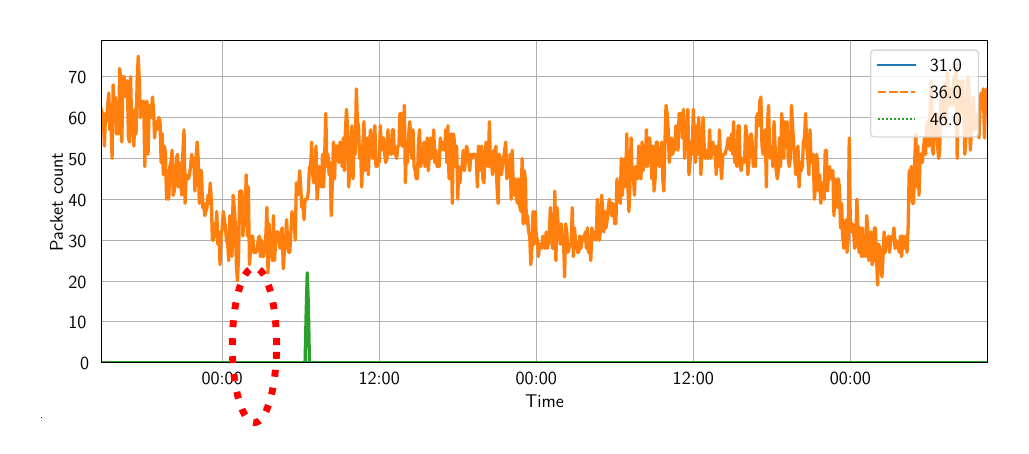
\begin{tikzpicture}
            \node(A){   
            \resizebox{1\textwidth}{!}
                {
                    %% Creator: Matplotlib, PGF backend
%%
%% To include the figure in your LaTeX document, write
%%   \input{<filename>.pgf}
%%
%% Make sure the required packages are loaded in your preamble
%%   \usepackage{pgf}
%%
%% Also ensure that all the required font packages are loaded; for instance,
%% the lmodern package is sometimes necessary when using math font.
%%   \usepackage{lmodern}
%%
%% Figures using additional raster images can only be included by \input if
%% they are in the same directory as the main LaTeX file. For loading figures
%% from other directories you can use the `import` package
%%   \usepackage{import}
%%
%% and then include the figures with
%%   \import{<path to file>}{<filename>.pgf}
%%
%% Matplotlib used the following preamble
%%   \usepackage{fontspec}
%%   \setmainfont{DejaVuSerif.ttf}[Path=\detokenize{/home/ankimme/fit/ibt/env/lib/python3.10/site-packages/matplotlib/mpl-data/fonts/ttf/}]
%%   \setsansfont{DejaVuSans.ttf}[Path=\detokenize{/home/ankimme/fit/ibt/env/lib/python3.10/site-packages/matplotlib/mpl-data/fonts/ttf/}]
%%   \setmonofont{DejaVuSansMono.ttf}[Path=\detokenize{/home/ankimme/fit/ibt/env/lib/python3.10/site-packages/matplotlib/mpl-data/fonts/ttf/}]
%%
\begingroup%
\makeatletter%
\begin{pgfpicture}%
\pgfpathrectangle{\pgfpointorigin}{\pgfqpoint{10.000000in}{4.000000in}}%
\pgfusepath{use as bounding box, clip}%
\begin{pgfscope}%
\pgfsetbuttcap%
\pgfsetmiterjoin%
\pgfsetlinewidth{0.000000pt}%
\definecolor{currentstroke}{rgb}{1.000000,1.000000,1.000000}%
\pgfsetstrokecolor{currentstroke}%
\pgfsetstrokeopacity{0.000000}%
\pgfsetdash{}{0pt}%
\pgfpathmoveto{\pgfqpoint{0.000000in}{0.000000in}}%
\pgfpathlineto{\pgfqpoint{10.000000in}{0.000000in}}%
\pgfpathlineto{\pgfqpoint{10.000000in}{4.000000in}}%
\pgfpathlineto{\pgfqpoint{0.000000in}{4.000000in}}%
\pgfpathlineto{\pgfqpoint{0.000000in}{0.000000in}}%
\pgfpathclose%
\pgfusepath{}%
\end{pgfscope}%
\begin{pgfscope}%
\pgfsetbuttcap%
\pgfsetmiterjoin%
\definecolor{currentfill}{rgb}{1.000000,1.000000,1.000000}%
\pgfsetfillcolor{currentfill}%
\pgfsetlinewidth{0.000000pt}%
\definecolor{currentstroke}{rgb}{0.000000,0.000000,0.000000}%
\pgfsetstrokecolor{currentstroke}%
\pgfsetstrokeopacity{0.000000}%
\pgfsetdash{}{0pt}%
\pgfpathmoveto{\pgfqpoint{0.630049in}{0.570804in}}%
\pgfpathlineto{\pgfqpoint{9.958330in}{0.570804in}}%
\pgfpathlineto{\pgfqpoint{9.958330in}{3.958330in}}%
\pgfpathlineto{\pgfqpoint{0.630049in}{3.958330in}}%
\pgfpathlineto{\pgfqpoint{0.630049in}{0.570804in}}%
\pgfpathclose%
\pgfusepath{fill}%
\end{pgfscope}%
\begin{pgfscope}%
\pgfpathrectangle{\pgfqpoint{0.630049in}{0.570804in}}{\pgfqpoint{9.328281in}{3.387526in}}%
\pgfusepath{clip}%
\pgfsetrectcap%
\pgfsetroundjoin%
\pgfsetlinewidth{0.803000pt}%
\definecolor{currentstroke}{rgb}{0.690196,0.690196,0.690196}%
\pgfsetstrokecolor{currentstroke}%
\pgfsetdash{}{0pt}%
\pgfpathmoveto{\pgfqpoint{1.903652in}{0.570804in}}%
\pgfpathlineto{\pgfqpoint{1.903652in}{3.958330in}}%
\pgfusepath{stroke}%
\end{pgfscope}%
\begin{pgfscope}%
\pgfsetbuttcap%
\pgfsetroundjoin%
\definecolor{currentfill}{rgb}{0.000000,0.000000,0.000000}%
\pgfsetfillcolor{currentfill}%
\pgfsetlinewidth{0.803000pt}%
\definecolor{currentstroke}{rgb}{0.000000,0.000000,0.000000}%
\pgfsetstrokecolor{currentstroke}%
\pgfsetdash{}{0pt}%
\pgfsys@defobject{currentmarker}{\pgfqpoint{0.000000in}{-0.048611in}}{\pgfqpoint{0.000000in}{0.000000in}}{%
\pgfpathmoveto{\pgfqpoint{0.000000in}{0.000000in}}%
\pgfpathlineto{\pgfqpoint{0.000000in}{-0.048611in}}%
\pgfusepath{stroke,fill}%
}%
\begin{pgfscope}%
\pgfsys@transformshift{1.903652in}{0.570804in}%
\pgfsys@useobject{currentmarker}{}%
\end{pgfscope}%
\end{pgfscope}%
\begin{pgfscope}%
\definecolor{textcolor}{rgb}{0.000000,0.000000,0.000000}%
\pgfsetstrokecolor{textcolor}%
\pgfsetfillcolor{textcolor}%
\pgftext[x=1.903652in,y=0.473582in,,top]{\color{textcolor}\sffamily\fontsize{14.000000}{16.800000}\selectfont 00:00}%
\end{pgfscope}%
\begin{pgfscope}%
\pgfpathrectangle{\pgfqpoint{0.630049in}{0.570804in}}{\pgfqpoint{9.328281in}{3.387526in}}%
\pgfusepath{clip}%
\pgfsetrectcap%
\pgfsetroundjoin%
\pgfsetlinewidth{0.803000pt}%
\definecolor{currentstroke}{rgb}{0.690196,0.690196,0.690196}%
\pgfsetstrokecolor{currentstroke}%
\pgfsetdash{}{0pt}%
\pgfpathmoveto{\pgfqpoint{3.555893in}{0.570804in}}%
\pgfpathlineto{\pgfqpoint{3.555893in}{3.958330in}}%
\pgfusepath{stroke}%
\end{pgfscope}%
\begin{pgfscope}%
\pgfsetbuttcap%
\pgfsetroundjoin%
\definecolor{currentfill}{rgb}{0.000000,0.000000,0.000000}%
\pgfsetfillcolor{currentfill}%
\pgfsetlinewidth{0.803000pt}%
\definecolor{currentstroke}{rgb}{0.000000,0.000000,0.000000}%
\pgfsetstrokecolor{currentstroke}%
\pgfsetdash{}{0pt}%
\pgfsys@defobject{currentmarker}{\pgfqpoint{0.000000in}{-0.048611in}}{\pgfqpoint{0.000000in}{0.000000in}}{%
\pgfpathmoveto{\pgfqpoint{0.000000in}{0.000000in}}%
\pgfpathlineto{\pgfqpoint{0.000000in}{-0.048611in}}%
\pgfusepath{stroke,fill}%
}%
\begin{pgfscope}%
\pgfsys@transformshift{3.555893in}{0.570804in}%
\pgfsys@useobject{currentmarker}{}%
\end{pgfscope}%
\end{pgfscope}%
\begin{pgfscope}%
\definecolor{textcolor}{rgb}{0.000000,0.000000,0.000000}%
\pgfsetstrokecolor{textcolor}%
\pgfsetfillcolor{textcolor}%
\pgftext[x=3.555893in,y=0.473582in,,top]{\color{textcolor}\sffamily\fontsize{14.000000}{16.800000}\selectfont 12:00}%
\end{pgfscope}%
\begin{pgfscope}%
\pgfpathrectangle{\pgfqpoint{0.630049in}{0.570804in}}{\pgfqpoint{9.328281in}{3.387526in}}%
\pgfusepath{clip}%
\pgfsetrectcap%
\pgfsetroundjoin%
\pgfsetlinewidth{0.803000pt}%
\definecolor{currentstroke}{rgb}{0.690196,0.690196,0.690196}%
\pgfsetstrokecolor{currentstroke}%
\pgfsetdash{}{0pt}%
\pgfpathmoveto{\pgfqpoint{5.208135in}{0.570804in}}%
\pgfpathlineto{\pgfqpoint{5.208135in}{3.958330in}}%
\pgfusepath{stroke}%
\end{pgfscope}%
\begin{pgfscope}%
\pgfsetbuttcap%
\pgfsetroundjoin%
\definecolor{currentfill}{rgb}{0.000000,0.000000,0.000000}%
\pgfsetfillcolor{currentfill}%
\pgfsetlinewidth{0.803000pt}%
\definecolor{currentstroke}{rgb}{0.000000,0.000000,0.000000}%
\pgfsetstrokecolor{currentstroke}%
\pgfsetdash{}{0pt}%
\pgfsys@defobject{currentmarker}{\pgfqpoint{0.000000in}{-0.048611in}}{\pgfqpoint{0.000000in}{0.000000in}}{%
\pgfpathmoveto{\pgfqpoint{0.000000in}{0.000000in}}%
\pgfpathlineto{\pgfqpoint{0.000000in}{-0.048611in}}%
\pgfusepath{stroke,fill}%
}%
\begin{pgfscope}%
\pgfsys@transformshift{5.208135in}{0.570804in}%
\pgfsys@useobject{currentmarker}{}%
\end{pgfscope}%
\end{pgfscope}%
\begin{pgfscope}%
\definecolor{textcolor}{rgb}{0.000000,0.000000,0.000000}%
\pgfsetstrokecolor{textcolor}%
\pgfsetfillcolor{textcolor}%
\pgftext[x=5.208135in,y=0.473582in,,top]{\color{textcolor}\sffamily\fontsize{14.000000}{16.800000}\selectfont 00:00}%
\end{pgfscope}%
\begin{pgfscope}%
\pgfpathrectangle{\pgfqpoint{0.630049in}{0.570804in}}{\pgfqpoint{9.328281in}{3.387526in}}%
\pgfusepath{clip}%
\pgfsetrectcap%
\pgfsetroundjoin%
\pgfsetlinewidth{0.803000pt}%
\definecolor{currentstroke}{rgb}{0.690196,0.690196,0.690196}%
\pgfsetstrokecolor{currentstroke}%
\pgfsetdash{}{0pt}%
\pgfpathmoveto{\pgfqpoint{6.860377in}{0.570804in}}%
\pgfpathlineto{\pgfqpoint{6.860377in}{3.958330in}}%
\pgfusepath{stroke}%
\end{pgfscope}%
\begin{pgfscope}%
\pgfsetbuttcap%
\pgfsetroundjoin%
\definecolor{currentfill}{rgb}{0.000000,0.000000,0.000000}%
\pgfsetfillcolor{currentfill}%
\pgfsetlinewidth{0.803000pt}%
\definecolor{currentstroke}{rgb}{0.000000,0.000000,0.000000}%
\pgfsetstrokecolor{currentstroke}%
\pgfsetdash{}{0pt}%
\pgfsys@defobject{currentmarker}{\pgfqpoint{0.000000in}{-0.048611in}}{\pgfqpoint{0.000000in}{0.000000in}}{%
\pgfpathmoveto{\pgfqpoint{0.000000in}{0.000000in}}%
\pgfpathlineto{\pgfqpoint{0.000000in}{-0.048611in}}%
\pgfusepath{stroke,fill}%
}%
\begin{pgfscope}%
\pgfsys@transformshift{6.860377in}{0.570804in}%
\pgfsys@useobject{currentmarker}{}%
\end{pgfscope}%
\end{pgfscope}%
\begin{pgfscope}%
\definecolor{textcolor}{rgb}{0.000000,0.000000,0.000000}%
\pgfsetstrokecolor{textcolor}%
\pgfsetfillcolor{textcolor}%
\pgftext[x=6.860377in,y=0.473582in,,top]{\color{textcolor}\sffamily\fontsize{14.000000}{16.800000}\selectfont 12:00}%
\end{pgfscope}%
\begin{pgfscope}%
\pgfpathrectangle{\pgfqpoint{0.630049in}{0.570804in}}{\pgfqpoint{9.328281in}{3.387526in}}%
\pgfusepath{clip}%
\pgfsetrectcap%
\pgfsetroundjoin%
\pgfsetlinewidth{0.803000pt}%
\definecolor{currentstroke}{rgb}{0.690196,0.690196,0.690196}%
\pgfsetstrokecolor{currentstroke}%
\pgfsetdash{}{0pt}%
\pgfpathmoveto{\pgfqpoint{8.512619in}{0.570804in}}%
\pgfpathlineto{\pgfqpoint{8.512619in}{3.958330in}}%
\pgfusepath{stroke}%
\end{pgfscope}%
\begin{pgfscope}%
\pgfsetbuttcap%
\pgfsetroundjoin%
\definecolor{currentfill}{rgb}{0.000000,0.000000,0.000000}%
\pgfsetfillcolor{currentfill}%
\pgfsetlinewidth{0.803000pt}%
\definecolor{currentstroke}{rgb}{0.000000,0.000000,0.000000}%
\pgfsetstrokecolor{currentstroke}%
\pgfsetdash{}{0pt}%
\pgfsys@defobject{currentmarker}{\pgfqpoint{0.000000in}{-0.048611in}}{\pgfqpoint{0.000000in}{0.000000in}}{%
\pgfpathmoveto{\pgfqpoint{0.000000in}{0.000000in}}%
\pgfpathlineto{\pgfqpoint{0.000000in}{-0.048611in}}%
\pgfusepath{stroke,fill}%
}%
\begin{pgfscope}%
\pgfsys@transformshift{8.512619in}{0.570804in}%
\pgfsys@useobject{currentmarker}{}%
\end{pgfscope}%
\end{pgfscope}%
\begin{pgfscope}%
\definecolor{textcolor}{rgb}{0.000000,0.000000,0.000000}%
\pgfsetstrokecolor{textcolor}%
\pgfsetfillcolor{textcolor}%
\pgftext[x=8.512619in,y=0.473582in,,top]{\color{textcolor}\sffamily\fontsize{14.000000}{16.800000}\selectfont 00:00}%
\end{pgfscope}%
\begin{pgfscope}%
\definecolor{textcolor}{rgb}{0.000000,0.000000,0.000000}%
\pgfsetstrokecolor{textcolor}%
\pgfsetfillcolor{textcolor}%
\pgftext[x=5.294189in,y=0.229848in,,top]{\color{textcolor}\sffamily\fontsize{14.000000}{16.800000}\selectfont Time}%
\end{pgfscope}%
\begin{pgfscope}%
\pgfpathrectangle{\pgfqpoint{0.630049in}{0.570804in}}{\pgfqpoint{9.328281in}{3.387526in}}%
\pgfusepath{clip}%
\pgfsetrectcap%
\pgfsetroundjoin%
\pgfsetlinewidth{0.803000pt}%
\definecolor{currentstroke}{rgb}{0.690196,0.690196,0.690196}%
\pgfsetstrokecolor{currentstroke}%
\pgfsetdash{}{0pt}%
\pgfpathmoveto{\pgfqpoint{0.630049in}{0.570804in}}%
\pgfpathlineto{\pgfqpoint{9.958330in}{0.570804in}}%
\pgfusepath{stroke}%
\end{pgfscope}%
\begin{pgfscope}%
\pgfsetbuttcap%
\pgfsetroundjoin%
\definecolor{currentfill}{rgb}{0.000000,0.000000,0.000000}%
\pgfsetfillcolor{currentfill}%
\pgfsetlinewidth{0.803000pt}%
\definecolor{currentstroke}{rgb}{0.000000,0.000000,0.000000}%
\pgfsetstrokecolor{currentstroke}%
\pgfsetdash{}{0pt}%
\pgfsys@defobject{currentmarker}{\pgfqpoint{-0.048611in}{0.000000in}}{\pgfqpoint{-0.000000in}{0.000000in}}{%
\pgfpathmoveto{\pgfqpoint{-0.000000in}{0.000000in}}%
\pgfpathlineto{\pgfqpoint{-0.048611in}{0.000000in}}%
\pgfusepath{stroke,fill}%
}%
\begin{pgfscope}%
\pgfsys@transformshift{0.630049in}{0.570804in}%
\pgfsys@useobject{currentmarker}{}%
\end{pgfscope}%
\end{pgfscope}%
\begin{pgfscope}%
\definecolor{textcolor}{rgb}{0.000000,0.000000,0.000000}%
\pgfsetstrokecolor{textcolor}%
\pgfsetfillcolor{textcolor}%
\pgftext[x=0.409115in, y=0.496938in, left, base]{\color{textcolor}\sffamily\fontsize{14.000000}{16.800000}\selectfont 0}%
\end{pgfscope}%
\begin{pgfscope}%
\pgfpathrectangle{\pgfqpoint{0.630049in}{0.570804in}}{\pgfqpoint{9.328281in}{3.387526in}}%
\pgfusepath{clip}%
\pgfsetrectcap%
\pgfsetroundjoin%
\pgfsetlinewidth{0.803000pt}%
\definecolor{currentstroke}{rgb}{0.690196,0.690196,0.690196}%
\pgfsetstrokecolor{currentstroke}%
\pgfsetdash{}{0pt}%
\pgfpathmoveto{\pgfqpoint{0.630049in}{1.000966in}}%
\pgfpathlineto{\pgfqpoint{9.958330in}{1.000966in}}%
\pgfusepath{stroke}%
\end{pgfscope}%
\begin{pgfscope}%
\pgfsetbuttcap%
\pgfsetroundjoin%
\definecolor{currentfill}{rgb}{0.000000,0.000000,0.000000}%
\pgfsetfillcolor{currentfill}%
\pgfsetlinewidth{0.803000pt}%
\definecolor{currentstroke}{rgb}{0.000000,0.000000,0.000000}%
\pgfsetstrokecolor{currentstroke}%
\pgfsetdash{}{0pt}%
\pgfsys@defobject{currentmarker}{\pgfqpoint{-0.048611in}{0.000000in}}{\pgfqpoint{-0.000000in}{0.000000in}}{%
\pgfpathmoveto{\pgfqpoint{-0.000000in}{0.000000in}}%
\pgfpathlineto{\pgfqpoint{-0.048611in}{0.000000in}}%
\pgfusepath{stroke,fill}%
}%
\begin{pgfscope}%
\pgfsys@transformshift{0.630049in}{1.000966in}%
\pgfsys@useobject{currentmarker}{}%
\end{pgfscope}%
\end{pgfscope}%
\begin{pgfscope}%
\definecolor{textcolor}{rgb}{0.000000,0.000000,0.000000}%
\pgfsetstrokecolor{textcolor}%
\pgfsetfillcolor{textcolor}%
\pgftext[x=0.285404in, y=0.927100in, left, base]{\color{textcolor}\sffamily\fontsize{14.000000}{16.800000}\selectfont 10}%
\end{pgfscope}%
\begin{pgfscope}%
\pgfpathrectangle{\pgfqpoint{0.630049in}{0.570804in}}{\pgfqpoint{9.328281in}{3.387526in}}%
\pgfusepath{clip}%
\pgfsetrectcap%
\pgfsetroundjoin%
\pgfsetlinewidth{0.803000pt}%
\definecolor{currentstroke}{rgb}{0.690196,0.690196,0.690196}%
\pgfsetstrokecolor{currentstroke}%
\pgfsetdash{}{0pt}%
\pgfpathmoveto{\pgfqpoint{0.630049in}{1.431128in}}%
\pgfpathlineto{\pgfqpoint{9.958330in}{1.431128in}}%
\pgfusepath{stroke}%
\end{pgfscope}%
\begin{pgfscope}%
\pgfsetbuttcap%
\pgfsetroundjoin%
\definecolor{currentfill}{rgb}{0.000000,0.000000,0.000000}%
\pgfsetfillcolor{currentfill}%
\pgfsetlinewidth{0.803000pt}%
\definecolor{currentstroke}{rgb}{0.000000,0.000000,0.000000}%
\pgfsetstrokecolor{currentstroke}%
\pgfsetdash{}{0pt}%
\pgfsys@defobject{currentmarker}{\pgfqpoint{-0.048611in}{0.000000in}}{\pgfqpoint{-0.000000in}{0.000000in}}{%
\pgfpathmoveto{\pgfqpoint{-0.000000in}{0.000000in}}%
\pgfpathlineto{\pgfqpoint{-0.048611in}{0.000000in}}%
\pgfusepath{stroke,fill}%
}%
\begin{pgfscope}%
\pgfsys@transformshift{0.630049in}{1.431128in}%
\pgfsys@useobject{currentmarker}{}%
\end{pgfscope}%
\end{pgfscope}%
\begin{pgfscope}%
\definecolor{textcolor}{rgb}{0.000000,0.000000,0.000000}%
\pgfsetstrokecolor{textcolor}%
\pgfsetfillcolor{textcolor}%
\pgftext[x=0.285404in, y=1.357262in, left, base]{\color{textcolor}\sffamily\fontsize{14.000000}{16.800000}\selectfont 20}%
\end{pgfscope}%
\begin{pgfscope}%
\pgfpathrectangle{\pgfqpoint{0.630049in}{0.570804in}}{\pgfqpoint{9.328281in}{3.387526in}}%
\pgfusepath{clip}%
\pgfsetrectcap%
\pgfsetroundjoin%
\pgfsetlinewidth{0.803000pt}%
\definecolor{currentstroke}{rgb}{0.690196,0.690196,0.690196}%
\pgfsetstrokecolor{currentstroke}%
\pgfsetdash{}{0pt}%
\pgfpathmoveto{\pgfqpoint{0.630049in}{1.861290in}}%
\pgfpathlineto{\pgfqpoint{9.958330in}{1.861290in}}%
\pgfusepath{stroke}%
\end{pgfscope}%
\begin{pgfscope}%
\pgfsetbuttcap%
\pgfsetroundjoin%
\definecolor{currentfill}{rgb}{0.000000,0.000000,0.000000}%
\pgfsetfillcolor{currentfill}%
\pgfsetlinewidth{0.803000pt}%
\definecolor{currentstroke}{rgb}{0.000000,0.000000,0.000000}%
\pgfsetstrokecolor{currentstroke}%
\pgfsetdash{}{0pt}%
\pgfsys@defobject{currentmarker}{\pgfqpoint{-0.048611in}{0.000000in}}{\pgfqpoint{-0.000000in}{0.000000in}}{%
\pgfpathmoveto{\pgfqpoint{-0.000000in}{0.000000in}}%
\pgfpathlineto{\pgfqpoint{-0.048611in}{0.000000in}}%
\pgfusepath{stroke,fill}%
}%
\begin{pgfscope}%
\pgfsys@transformshift{0.630049in}{1.861290in}%
\pgfsys@useobject{currentmarker}{}%
\end{pgfscope}%
\end{pgfscope}%
\begin{pgfscope}%
\definecolor{textcolor}{rgb}{0.000000,0.000000,0.000000}%
\pgfsetstrokecolor{textcolor}%
\pgfsetfillcolor{textcolor}%
\pgftext[x=0.285404in, y=1.787424in, left, base]{\color{textcolor}\sffamily\fontsize{14.000000}{16.800000}\selectfont 30}%
\end{pgfscope}%
\begin{pgfscope}%
\pgfpathrectangle{\pgfqpoint{0.630049in}{0.570804in}}{\pgfqpoint{9.328281in}{3.387526in}}%
\pgfusepath{clip}%
\pgfsetrectcap%
\pgfsetroundjoin%
\pgfsetlinewidth{0.803000pt}%
\definecolor{currentstroke}{rgb}{0.690196,0.690196,0.690196}%
\pgfsetstrokecolor{currentstroke}%
\pgfsetdash{}{0pt}%
\pgfpathmoveto{\pgfqpoint{0.630049in}{2.291452in}}%
\pgfpathlineto{\pgfqpoint{9.958330in}{2.291452in}}%
\pgfusepath{stroke}%
\end{pgfscope}%
\begin{pgfscope}%
\pgfsetbuttcap%
\pgfsetroundjoin%
\definecolor{currentfill}{rgb}{0.000000,0.000000,0.000000}%
\pgfsetfillcolor{currentfill}%
\pgfsetlinewidth{0.803000pt}%
\definecolor{currentstroke}{rgb}{0.000000,0.000000,0.000000}%
\pgfsetstrokecolor{currentstroke}%
\pgfsetdash{}{0pt}%
\pgfsys@defobject{currentmarker}{\pgfqpoint{-0.048611in}{0.000000in}}{\pgfqpoint{-0.000000in}{0.000000in}}{%
\pgfpathmoveto{\pgfqpoint{-0.000000in}{0.000000in}}%
\pgfpathlineto{\pgfqpoint{-0.048611in}{0.000000in}}%
\pgfusepath{stroke,fill}%
}%
\begin{pgfscope}%
\pgfsys@transformshift{0.630049in}{2.291452in}%
\pgfsys@useobject{currentmarker}{}%
\end{pgfscope}%
\end{pgfscope}%
\begin{pgfscope}%
\definecolor{textcolor}{rgb}{0.000000,0.000000,0.000000}%
\pgfsetstrokecolor{textcolor}%
\pgfsetfillcolor{textcolor}%
\pgftext[x=0.285404in, y=2.217586in, left, base]{\color{textcolor}\sffamily\fontsize{14.000000}{16.800000}\selectfont 40}%
\end{pgfscope}%
\begin{pgfscope}%
\pgfpathrectangle{\pgfqpoint{0.630049in}{0.570804in}}{\pgfqpoint{9.328281in}{3.387526in}}%
\pgfusepath{clip}%
\pgfsetrectcap%
\pgfsetroundjoin%
\pgfsetlinewidth{0.803000pt}%
\definecolor{currentstroke}{rgb}{0.690196,0.690196,0.690196}%
\pgfsetstrokecolor{currentstroke}%
\pgfsetdash{}{0pt}%
\pgfpathmoveto{\pgfqpoint{0.630049in}{2.721614in}}%
\pgfpathlineto{\pgfqpoint{9.958330in}{2.721614in}}%
\pgfusepath{stroke}%
\end{pgfscope}%
\begin{pgfscope}%
\pgfsetbuttcap%
\pgfsetroundjoin%
\definecolor{currentfill}{rgb}{0.000000,0.000000,0.000000}%
\pgfsetfillcolor{currentfill}%
\pgfsetlinewidth{0.803000pt}%
\definecolor{currentstroke}{rgb}{0.000000,0.000000,0.000000}%
\pgfsetstrokecolor{currentstroke}%
\pgfsetdash{}{0pt}%
\pgfsys@defobject{currentmarker}{\pgfqpoint{-0.048611in}{0.000000in}}{\pgfqpoint{-0.000000in}{0.000000in}}{%
\pgfpathmoveto{\pgfqpoint{-0.000000in}{0.000000in}}%
\pgfpathlineto{\pgfqpoint{-0.048611in}{0.000000in}}%
\pgfusepath{stroke,fill}%
}%
\begin{pgfscope}%
\pgfsys@transformshift{0.630049in}{2.721614in}%
\pgfsys@useobject{currentmarker}{}%
\end{pgfscope}%
\end{pgfscope}%
\begin{pgfscope}%
\definecolor{textcolor}{rgb}{0.000000,0.000000,0.000000}%
\pgfsetstrokecolor{textcolor}%
\pgfsetfillcolor{textcolor}%
\pgftext[x=0.285404in, y=2.647748in, left, base]{\color{textcolor}\sffamily\fontsize{14.000000}{16.800000}\selectfont 50}%
\end{pgfscope}%
\begin{pgfscope}%
\pgfpathrectangle{\pgfqpoint{0.630049in}{0.570804in}}{\pgfqpoint{9.328281in}{3.387526in}}%
\pgfusepath{clip}%
\pgfsetrectcap%
\pgfsetroundjoin%
\pgfsetlinewidth{0.803000pt}%
\definecolor{currentstroke}{rgb}{0.690196,0.690196,0.690196}%
\pgfsetstrokecolor{currentstroke}%
\pgfsetdash{}{0pt}%
\pgfpathmoveto{\pgfqpoint{0.630049in}{3.151776in}}%
\pgfpathlineto{\pgfqpoint{9.958330in}{3.151776in}}%
\pgfusepath{stroke}%
\end{pgfscope}%
\begin{pgfscope}%
\pgfsetbuttcap%
\pgfsetroundjoin%
\definecolor{currentfill}{rgb}{0.000000,0.000000,0.000000}%
\pgfsetfillcolor{currentfill}%
\pgfsetlinewidth{0.803000pt}%
\definecolor{currentstroke}{rgb}{0.000000,0.000000,0.000000}%
\pgfsetstrokecolor{currentstroke}%
\pgfsetdash{}{0pt}%
\pgfsys@defobject{currentmarker}{\pgfqpoint{-0.048611in}{0.000000in}}{\pgfqpoint{-0.000000in}{0.000000in}}{%
\pgfpathmoveto{\pgfqpoint{-0.000000in}{0.000000in}}%
\pgfpathlineto{\pgfqpoint{-0.048611in}{0.000000in}}%
\pgfusepath{stroke,fill}%
}%
\begin{pgfscope}%
\pgfsys@transformshift{0.630049in}{3.151776in}%
\pgfsys@useobject{currentmarker}{}%
\end{pgfscope}%
\end{pgfscope}%
\begin{pgfscope}%
\definecolor{textcolor}{rgb}{0.000000,0.000000,0.000000}%
\pgfsetstrokecolor{textcolor}%
\pgfsetfillcolor{textcolor}%
\pgftext[x=0.285404in, y=3.077910in, left, base]{\color{textcolor}\sffamily\fontsize{14.000000}{16.800000}\selectfont 60}%
\end{pgfscope}%
\begin{pgfscope}%
\pgfpathrectangle{\pgfqpoint{0.630049in}{0.570804in}}{\pgfqpoint{9.328281in}{3.387526in}}%
\pgfusepath{clip}%
\pgfsetrectcap%
\pgfsetroundjoin%
\pgfsetlinewidth{0.803000pt}%
\definecolor{currentstroke}{rgb}{0.690196,0.690196,0.690196}%
\pgfsetstrokecolor{currentstroke}%
\pgfsetdash{}{0pt}%
\pgfpathmoveto{\pgfqpoint{0.630049in}{3.581938in}}%
\pgfpathlineto{\pgfqpoint{9.958330in}{3.581938in}}%
\pgfusepath{stroke}%
\end{pgfscope}%
\begin{pgfscope}%
\pgfsetbuttcap%
\pgfsetroundjoin%
\definecolor{currentfill}{rgb}{0.000000,0.000000,0.000000}%
\pgfsetfillcolor{currentfill}%
\pgfsetlinewidth{0.803000pt}%
\definecolor{currentstroke}{rgb}{0.000000,0.000000,0.000000}%
\pgfsetstrokecolor{currentstroke}%
\pgfsetdash{}{0pt}%
\pgfsys@defobject{currentmarker}{\pgfqpoint{-0.048611in}{0.000000in}}{\pgfqpoint{-0.000000in}{0.000000in}}{%
\pgfpathmoveto{\pgfqpoint{-0.000000in}{0.000000in}}%
\pgfpathlineto{\pgfqpoint{-0.048611in}{0.000000in}}%
\pgfusepath{stroke,fill}%
}%
\begin{pgfscope}%
\pgfsys@transformshift{0.630049in}{3.581938in}%
\pgfsys@useobject{currentmarker}{}%
\end{pgfscope}%
\end{pgfscope}%
\begin{pgfscope}%
\definecolor{textcolor}{rgb}{0.000000,0.000000,0.000000}%
\pgfsetstrokecolor{textcolor}%
\pgfsetfillcolor{textcolor}%
\pgftext[x=0.285404in, y=3.508072in, left, base]{\color{textcolor}\sffamily\fontsize{14.000000}{16.800000}\selectfont 70}%
\end{pgfscope}%
\begin{pgfscope}%
\definecolor{textcolor}{rgb}{0.000000,0.000000,0.000000}%
\pgfsetstrokecolor{textcolor}%
\pgfsetfillcolor{textcolor}%
\pgftext[x=0.229848in,y=2.264567in,,bottom,rotate=90.000000]{\color{textcolor}\sffamily\fontsize{14.000000}{16.800000}\selectfont Packet count}%
\end{pgfscope}%
\begin{pgfscope}%
\pgfpathrectangle{\pgfqpoint{0.630049in}{0.570804in}}{\pgfqpoint{9.328281in}{3.387526in}}%
\pgfusepath{clip}%
\pgfsetrectcap%
\pgfsetroundjoin%
\pgfsetlinewidth{2.509375pt}%
\definecolor{currentstroke}{rgb}{0.121569,0.466667,0.705882}%
\pgfsetstrokecolor{currentstroke}%
\pgfsetdash{}{0pt}%
\pgfpathmoveto{\pgfqpoint{0.630049in}{0.570804in}}%
\pgfpathlineto{\pgfqpoint{9.958330in}{0.570804in}}%
\pgfpathlineto{\pgfqpoint{9.958330in}{0.570804in}}%
\pgfusepath{stroke}%
\end{pgfscope}%
\begin{pgfscope}%
\pgfpathrectangle{\pgfqpoint{0.630049in}{0.570804in}}{\pgfqpoint{9.328281in}{3.387526in}}%
\pgfusepath{clip}%
\pgfsetrectcap%
\pgfsetroundjoin%
\pgfsetlinewidth{2.509375pt}%
\definecolor{currentstroke}{rgb}{1.000000,0.498039,0.054902}%
\pgfsetstrokecolor{currentstroke}%
\pgfsetdash{}{0pt}%
\pgfpathmoveto{\pgfqpoint{0.630049in}{3.237809in}}%
\pgfpathlineto{\pgfqpoint{0.652997in}{3.151776in}}%
\pgfpathlineto{\pgfqpoint{0.664470in}{2.850663in}}%
\pgfpathlineto{\pgfqpoint{0.675944in}{3.194792in}}%
\pgfpathlineto{\pgfqpoint{0.687418in}{3.108760in}}%
\pgfpathlineto{\pgfqpoint{0.698892in}{3.280825in}}%
\pgfpathlineto{\pgfqpoint{0.710366in}{3.409873in}}%
\pgfpathlineto{\pgfqpoint{0.721840in}{3.022728in}}%
\pgfpathlineto{\pgfqpoint{0.733314in}{3.108760in}}%
\pgfpathlineto{\pgfqpoint{0.744788in}{2.721614in}}%
\pgfpathlineto{\pgfqpoint{0.756262in}{3.495906in}}%
\pgfpathlineto{\pgfqpoint{0.767736in}{3.108760in}}%
\pgfpathlineto{\pgfqpoint{0.779209in}{3.366857in}}%
\pgfpathlineto{\pgfqpoint{0.790683in}{2.979711in}}%
\pgfpathlineto{\pgfqpoint{0.802157in}{3.022728in}}%
\pgfpathlineto{\pgfqpoint{0.813631in}{2.979711in}}%
\pgfpathlineto{\pgfqpoint{0.825105in}{3.667971in}}%
\pgfpathlineto{\pgfqpoint{0.836579in}{3.538922in}}%
\pgfpathlineto{\pgfqpoint{0.848053in}{2.893679in}}%
\pgfpathlineto{\pgfqpoint{0.859527in}{3.581938in}}%
\pgfpathlineto{\pgfqpoint{0.871001in}{3.581938in}}%
\pgfpathlineto{\pgfqpoint{0.882475in}{3.409873in}}%
\pgfpathlineto{\pgfqpoint{0.893948in}{3.366857in}}%
\pgfpathlineto{\pgfqpoint{0.905422in}{3.538922in}}%
\pgfpathlineto{\pgfqpoint{0.916896in}{2.936695in}}%
\pgfpathlineto{\pgfqpoint{0.928370in}{2.893679in}}%
\pgfpathlineto{\pgfqpoint{0.939844in}{3.581938in}}%
\pgfpathlineto{\pgfqpoint{0.951318in}{3.065744in}}%
\pgfpathlineto{\pgfqpoint{0.962792in}{3.065744in}}%
\pgfpathlineto{\pgfqpoint{0.974266in}{2.850663in}}%
\pgfpathlineto{\pgfqpoint{0.985740in}{3.237809in}}%
\pgfpathlineto{\pgfqpoint{0.997214in}{2.979711in}}%
\pgfpathlineto{\pgfqpoint{1.008687in}{3.538922in}}%
\pgfpathlineto{\pgfqpoint{1.020161in}{3.797019in}}%
\pgfpathlineto{\pgfqpoint{1.031635in}{3.538922in}}%
\pgfpathlineto{\pgfqpoint{1.043109in}{3.151776in}}%
\pgfpathlineto{\pgfqpoint{1.054583in}{3.323841in}}%
\pgfpathlineto{\pgfqpoint{1.066057in}{3.280825in}}%
\pgfpathlineto{\pgfqpoint{1.077531in}{3.323841in}}%
\pgfpathlineto{\pgfqpoint{1.089005in}{2.635582in}}%
\pgfpathlineto{\pgfqpoint{1.100479in}{3.108760in}}%
\pgfpathlineto{\pgfqpoint{1.111953in}{3.323841in}}%
\pgfpathlineto{\pgfqpoint{1.123426in}{2.764630in}}%
\pgfpathlineto{\pgfqpoint{1.134900in}{3.280825in}}%
\pgfpathlineto{\pgfqpoint{1.146374in}{3.237809in}}%
\pgfpathlineto{\pgfqpoint{1.157848in}{3.151776in}}%
\pgfpathlineto{\pgfqpoint{1.169322in}{3.366857in}}%
\pgfpathlineto{\pgfqpoint{1.180796in}{3.237809in}}%
\pgfpathlineto{\pgfqpoint{1.192270in}{2.936695in}}%
\pgfpathlineto{\pgfqpoint{1.203744in}{3.108760in}}%
\pgfpathlineto{\pgfqpoint{1.215218in}{3.022728in}}%
\pgfpathlineto{\pgfqpoint{1.226692in}{3.108760in}}%
\pgfpathlineto{\pgfqpoint{1.238165in}{3.151776in}}%
\pgfpathlineto{\pgfqpoint{1.249639in}{3.108760in}}%
\pgfpathlineto{\pgfqpoint{1.261113in}{2.678598in}}%
\pgfpathlineto{\pgfqpoint{1.272587in}{2.979711in}}%
\pgfpathlineto{\pgfqpoint{1.284061in}{2.549549in}}%
\pgfpathlineto{\pgfqpoint{1.295535in}{2.850663in}}%
\pgfpathlineto{\pgfqpoint{1.307009in}{2.764630in}}%
\pgfpathlineto{\pgfqpoint{1.318483in}{2.291452in}}%
\pgfpathlineto{\pgfqpoint{1.329957in}{2.592566in}}%
\pgfpathlineto{\pgfqpoint{1.341431in}{2.291452in}}%
\pgfpathlineto{\pgfqpoint{1.352904in}{2.635582in}}%
\pgfpathlineto{\pgfqpoint{1.364378in}{2.678598in}}%
\pgfpathlineto{\pgfqpoint{1.375852in}{2.807647in}}%
\pgfpathlineto{\pgfqpoint{1.387326in}{2.334468in}}%
\pgfpathlineto{\pgfqpoint{1.398800in}{2.377484in}}%
\pgfpathlineto{\pgfqpoint{1.410274in}{2.463517in}}%
\pgfpathlineto{\pgfqpoint{1.421748in}{2.721614in}}%
\pgfpathlineto{\pgfqpoint{1.433222in}{2.764630in}}%
\pgfpathlineto{\pgfqpoint{1.444696in}{2.420501in}}%
\pgfpathlineto{\pgfqpoint{1.456170in}{2.678598in}}%
\pgfpathlineto{\pgfqpoint{1.467643in}{2.463517in}}%
\pgfpathlineto{\pgfqpoint{1.479117in}{2.334468in}}%
\pgfpathlineto{\pgfqpoint{1.490591in}{2.807647in}}%
\pgfpathlineto{\pgfqpoint{1.502065in}{3.022728in}}%
\pgfpathlineto{\pgfqpoint{1.513539in}{2.248436in}}%
\pgfpathlineto{\pgfqpoint{1.525013in}{2.549549in}}%
\pgfpathlineto{\pgfqpoint{1.536487in}{2.506533in}}%
\pgfpathlineto{\pgfqpoint{1.547961in}{2.506533in}}%
\pgfpathlineto{\pgfqpoint{1.559435in}{2.549549in}}%
\pgfpathlineto{\pgfqpoint{1.570909in}{2.635582in}}%
\pgfpathlineto{\pgfqpoint{1.582383in}{2.764630in}}%
\pgfpathlineto{\pgfqpoint{1.593856in}{2.678598in}}%
\pgfpathlineto{\pgfqpoint{1.605330in}{2.721614in}}%
\pgfpathlineto{\pgfqpoint{1.616804in}{2.377484in}}%
\pgfpathlineto{\pgfqpoint{1.628278in}{2.721614in}}%
\pgfpathlineto{\pgfqpoint{1.639752in}{2.893679in}}%
\pgfpathlineto{\pgfqpoint{1.651226in}{2.721614in}}%
\pgfpathlineto{\pgfqpoint{1.662700in}{2.248436in}}%
\pgfpathlineto{\pgfqpoint{1.674174in}{2.592566in}}%
\pgfpathlineto{\pgfqpoint{1.685648in}{2.592566in}}%
\pgfpathlineto{\pgfqpoint{1.697122in}{2.205420in}}%
\pgfpathlineto{\pgfqpoint{1.708595in}{2.248436in}}%
\pgfpathlineto{\pgfqpoint{1.720069in}{2.119387in}}%
\pgfpathlineto{\pgfqpoint{1.743017in}{2.205420in}}%
\pgfpathlineto{\pgfqpoint{1.754491in}{2.334468in}}%
\pgfpathlineto{\pgfqpoint{1.765965in}{2.248436in}}%
\pgfpathlineto{\pgfqpoint{1.777439in}{2.463517in}}%
\pgfpathlineto{\pgfqpoint{1.788913in}{2.291452in}}%
\pgfpathlineto{\pgfqpoint{1.800387in}{1.861290in}}%
\pgfpathlineto{\pgfqpoint{1.811861in}{1.861290in}}%
\pgfpathlineto{\pgfqpoint{1.823334in}{2.033355in}}%
\pgfpathlineto{\pgfqpoint{1.834808in}{1.904306in}}%
\pgfpathlineto{\pgfqpoint{1.846282in}{2.162403in}}%
\pgfpathlineto{\pgfqpoint{1.857756in}{1.818274in}}%
\pgfpathlineto{\pgfqpoint{1.869230in}{1.947322in}}%
\pgfpathlineto{\pgfqpoint{1.880704in}{1.603193in}}%
\pgfpathlineto{\pgfqpoint{1.892178in}{1.904306in}}%
\pgfpathlineto{\pgfqpoint{1.903652in}{1.990339in}}%
\pgfpathlineto{\pgfqpoint{1.915126in}{2.162403in}}%
\pgfpathlineto{\pgfqpoint{1.938073in}{1.990339in}}%
\pgfpathlineto{\pgfqpoint{1.949547in}{1.861290in}}%
\pgfpathlineto{\pgfqpoint{1.961021in}{1.818274in}}%
\pgfpathlineto{\pgfqpoint{1.972495in}{1.646209in}}%
\pgfpathlineto{\pgfqpoint{1.983969in}{2.119387in}}%
\pgfpathlineto{\pgfqpoint{1.995443in}{1.818274in}}%
\pgfpathlineto{\pgfqpoint{2.006917in}{1.689225in}}%
\pgfpathlineto{\pgfqpoint{2.018391in}{2.334468in}}%
\pgfpathlineto{\pgfqpoint{2.029865in}{2.205420in}}%
\pgfpathlineto{\pgfqpoint{2.041339in}{2.033355in}}%
\pgfpathlineto{\pgfqpoint{2.052812in}{1.603193in}}%
\pgfpathlineto{\pgfqpoint{2.064286in}{1.431128in}}%
\pgfpathlineto{\pgfqpoint{2.075760in}{1.689225in}}%
\pgfpathlineto{\pgfqpoint{2.087234in}{2.377484in}}%
\pgfpathlineto{\pgfqpoint{2.110182in}{2.377484in}}%
\pgfpathlineto{\pgfqpoint{2.121656in}{1.904306in}}%
\pgfpathlineto{\pgfqpoint{2.133130in}{2.162403in}}%
\pgfpathlineto{\pgfqpoint{2.144604in}{2.119387in}}%
\pgfpathlineto{\pgfqpoint{2.156078in}{2.549549in}}%
\pgfpathlineto{\pgfqpoint{2.167551in}{1.904306in}}%
\pgfpathlineto{\pgfqpoint{2.179025in}{2.420501in}}%
\pgfpathlineto{\pgfqpoint{2.190499in}{1.603193in}}%
\pgfpathlineto{\pgfqpoint{2.201973in}{1.775258in}}%
\pgfpathlineto{\pgfqpoint{2.213447in}{1.904306in}}%
\pgfpathlineto{\pgfqpoint{2.224921in}{1.904306in}}%
\pgfpathlineto{\pgfqpoint{2.236395in}{1.732241in}}%
\pgfpathlineto{\pgfqpoint{2.259343in}{1.732241in}}%
\pgfpathlineto{\pgfqpoint{2.270817in}{1.775258in}}%
\pgfpathlineto{\pgfqpoint{2.282290in}{1.861290in}}%
\pgfpathlineto{\pgfqpoint{2.293764in}{1.904306in}}%
\pgfpathlineto{\pgfqpoint{2.305238in}{1.689225in}}%
\pgfpathlineto{\pgfqpoint{2.316712in}{1.861290in}}%
\pgfpathlineto{\pgfqpoint{2.328186in}{1.689225in}}%
\pgfpathlineto{\pgfqpoint{2.339660in}{1.689225in}}%
\pgfpathlineto{\pgfqpoint{2.351134in}{1.775258in}}%
\pgfpathlineto{\pgfqpoint{2.362608in}{1.904306in}}%
\pgfpathlineto{\pgfqpoint{2.374082in}{2.205420in}}%
\pgfpathlineto{\pgfqpoint{2.385556in}{1.517160in}}%
\pgfpathlineto{\pgfqpoint{2.397029in}{2.033355in}}%
\pgfpathlineto{\pgfqpoint{2.408503in}{1.689225in}}%
\pgfpathlineto{\pgfqpoint{2.419977in}{1.732241in}}%
\pgfpathlineto{\pgfqpoint{2.431451in}{1.646209in}}%
\pgfpathlineto{\pgfqpoint{2.442925in}{2.119387in}}%
\pgfpathlineto{\pgfqpoint{2.454399in}{1.646209in}}%
\pgfpathlineto{\pgfqpoint{2.465873in}{1.861290in}}%
\pgfpathlineto{\pgfqpoint{2.477347in}{1.947322in}}%
\pgfpathlineto{\pgfqpoint{2.488821in}{1.947322in}}%
\pgfpathlineto{\pgfqpoint{2.511768in}{1.775258in}}%
\pgfpathlineto{\pgfqpoint{2.523242in}{1.947322in}}%
\pgfpathlineto{\pgfqpoint{2.534716in}{1.990339in}}%
\pgfpathlineto{\pgfqpoint{2.546190in}{1.560177in}}%
\pgfpathlineto{\pgfqpoint{2.557664in}{1.732241in}}%
\pgfpathlineto{\pgfqpoint{2.569138in}{1.818274in}}%
\pgfpathlineto{\pgfqpoint{2.580612in}{2.076371in}}%
\pgfpathlineto{\pgfqpoint{2.592086in}{1.861290in}}%
\pgfpathlineto{\pgfqpoint{2.603560in}{1.732241in}}%
\pgfpathlineto{\pgfqpoint{2.615034in}{1.732241in}}%
\pgfpathlineto{\pgfqpoint{2.637981in}{2.162403in}}%
\pgfpathlineto{\pgfqpoint{2.649455in}{1.990339in}}%
\pgfpathlineto{\pgfqpoint{2.660929in}{2.076371in}}%
\pgfpathlineto{\pgfqpoint{2.672403in}{1.861290in}}%
\pgfpathlineto{\pgfqpoint{2.683877in}{2.463517in}}%
\pgfpathlineto{\pgfqpoint{2.695351in}{2.334468in}}%
\pgfpathlineto{\pgfqpoint{2.706825in}{2.377484in}}%
\pgfpathlineto{\pgfqpoint{2.718299in}{2.592566in}}%
\pgfpathlineto{\pgfqpoint{2.729773in}{2.420501in}}%
\pgfpathlineto{\pgfqpoint{2.741246in}{2.205420in}}%
\pgfpathlineto{\pgfqpoint{2.752720in}{2.248436in}}%
\pgfpathlineto{\pgfqpoint{2.764194in}{2.076371in}}%
\pgfpathlineto{\pgfqpoint{2.775668in}{2.291452in}}%
\pgfpathlineto{\pgfqpoint{2.798616in}{2.291452in}}%
\pgfpathlineto{\pgfqpoint{2.810090in}{2.377484in}}%
\pgfpathlineto{\pgfqpoint{2.821564in}{2.635582in}}%
\pgfpathlineto{\pgfqpoint{2.833038in}{2.592566in}}%
\pgfpathlineto{\pgfqpoint{2.844512in}{2.893679in}}%
\pgfpathlineto{\pgfqpoint{2.855985in}{2.549549in}}%
\pgfpathlineto{\pgfqpoint{2.867459in}{2.463517in}}%
\pgfpathlineto{\pgfqpoint{2.878933in}{2.506533in}}%
\pgfpathlineto{\pgfqpoint{2.890407in}{2.850663in}}%
\pgfpathlineto{\pgfqpoint{2.901881in}{2.291452in}}%
\pgfpathlineto{\pgfqpoint{2.913355in}{2.420501in}}%
\pgfpathlineto{\pgfqpoint{2.924829in}{2.635582in}}%
\pgfpathlineto{\pgfqpoint{2.936303in}{2.549549in}}%
\pgfpathlineto{\pgfqpoint{2.947777in}{2.420501in}}%
\pgfpathlineto{\pgfqpoint{2.959251in}{2.764630in}}%
\pgfpathlineto{\pgfqpoint{2.970724in}{2.420501in}}%
\pgfpathlineto{\pgfqpoint{2.982198in}{2.764630in}}%
\pgfpathlineto{\pgfqpoint{2.993672in}{3.194792in}}%
\pgfpathlineto{\pgfqpoint{3.005146in}{2.635582in}}%
\pgfpathlineto{\pgfqpoint{3.016620in}{2.764630in}}%
\pgfpathlineto{\pgfqpoint{3.028094in}{2.549549in}}%
\pgfpathlineto{\pgfqpoint{3.039568in}{2.678598in}}%
\pgfpathlineto{\pgfqpoint{3.051042in}{2.119387in}}%
\pgfpathlineto{\pgfqpoint{3.062516in}{2.463517in}}%
\pgfpathlineto{\pgfqpoint{3.073990in}{2.893679in}}%
\pgfpathlineto{\pgfqpoint{3.085463in}{2.506533in}}%
\pgfpathlineto{\pgfqpoint{3.096937in}{2.850663in}}%
\pgfpathlineto{\pgfqpoint{3.108411in}{2.850663in}}%
\pgfpathlineto{\pgfqpoint{3.131359in}{2.678598in}}%
\pgfpathlineto{\pgfqpoint{3.142833in}{2.893679in}}%
\pgfpathlineto{\pgfqpoint{3.154307in}{2.807647in}}%
\pgfpathlineto{\pgfqpoint{3.165781in}{2.635582in}}%
\pgfpathlineto{\pgfqpoint{3.177255in}{2.936695in}}%
\pgfpathlineto{\pgfqpoint{3.188729in}{2.592566in}}%
\pgfpathlineto{\pgfqpoint{3.200203in}{3.022728in}}%
\pgfpathlineto{\pgfqpoint{3.211676in}{3.237809in}}%
\pgfpathlineto{\pgfqpoint{3.223150in}{3.022728in}}%
\pgfpathlineto{\pgfqpoint{3.234624in}{2.420501in}}%
\pgfpathlineto{\pgfqpoint{3.246098in}{2.592566in}}%
\pgfpathlineto{\pgfqpoint{3.257572in}{2.850663in}}%
\pgfpathlineto{\pgfqpoint{3.269046in}{3.065744in}}%
\pgfpathlineto{\pgfqpoint{3.280520in}{2.506533in}}%
\pgfpathlineto{\pgfqpoint{3.291994in}{2.979711in}}%
\pgfpathlineto{\pgfqpoint{3.303468in}{2.764630in}}%
\pgfpathlineto{\pgfqpoint{3.314942in}{3.452890in}}%
\pgfpathlineto{\pgfqpoint{3.326415in}{3.108760in}}%
\pgfpathlineto{\pgfqpoint{3.337889in}{3.065744in}}%
\pgfpathlineto{\pgfqpoint{3.349363in}{2.721614in}}%
\pgfpathlineto{\pgfqpoint{3.360837in}{2.764630in}}%
\pgfpathlineto{\pgfqpoint{3.372311in}{2.420501in}}%
\pgfpathlineto{\pgfqpoint{3.383785in}{2.850663in}}%
\pgfpathlineto{\pgfqpoint{3.395259in}{3.108760in}}%
\pgfpathlineto{\pgfqpoint{3.406733in}{2.592566in}}%
\pgfpathlineto{\pgfqpoint{3.418207in}{2.807647in}}%
\pgfpathlineto{\pgfqpoint{3.429681in}{2.936695in}}%
\pgfpathlineto{\pgfqpoint{3.441154in}{2.549549in}}%
\pgfpathlineto{\pgfqpoint{3.452628in}{2.850663in}}%
\pgfpathlineto{\pgfqpoint{3.464102in}{3.022728in}}%
\pgfpathlineto{\pgfqpoint{3.475576in}{2.893679in}}%
\pgfpathlineto{\pgfqpoint{3.487050in}{2.721614in}}%
\pgfpathlineto{\pgfqpoint{3.509998in}{3.065744in}}%
\pgfpathlineto{\pgfqpoint{3.521472in}{2.635582in}}%
\pgfpathlineto{\pgfqpoint{3.532946in}{2.635582in}}%
\pgfpathlineto{\pgfqpoint{3.544420in}{2.678598in}}%
\pgfpathlineto{\pgfqpoint{3.555893in}{2.678598in}}%
\pgfpathlineto{\pgfqpoint{3.567367in}{3.065744in}}%
\pgfpathlineto{\pgfqpoint{3.578841in}{2.807647in}}%
\pgfpathlineto{\pgfqpoint{3.590315in}{2.936695in}}%
\pgfpathlineto{\pgfqpoint{3.601789in}{2.936695in}}%
\pgfpathlineto{\pgfqpoint{3.613263in}{2.764630in}}%
\pgfpathlineto{\pgfqpoint{3.624737in}{2.678598in}}%
\pgfpathlineto{\pgfqpoint{3.636211in}{2.721614in}}%
\pgfpathlineto{\pgfqpoint{3.647685in}{3.022728in}}%
\pgfpathlineto{\pgfqpoint{3.659159in}{2.764630in}}%
\pgfpathlineto{\pgfqpoint{3.670632in}{2.807647in}}%
\pgfpathlineto{\pgfqpoint{3.682106in}{2.764630in}}%
\pgfpathlineto{\pgfqpoint{3.693580in}{3.022728in}}%
\pgfpathlineto{\pgfqpoint{3.705054in}{3.022728in}}%
\pgfpathlineto{\pgfqpoint{3.716528in}{2.764630in}}%
\pgfpathlineto{\pgfqpoint{3.728002in}{2.764630in}}%
\pgfpathlineto{\pgfqpoint{3.739476in}{2.721614in}}%
\pgfpathlineto{\pgfqpoint{3.750950in}{2.850663in}}%
\pgfpathlineto{\pgfqpoint{3.762424in}{2.850663in}}%
\pgfpathlineto{\pgfqpoint{3.773898in}{3.194792in}}%
\pgfpathlineto{\pgfqpoint{3.785371in}{3.194792in}}%
\pgfpathlineto{\pgfqpoint{3.796845in}{2.850663in}}%
\pgfpathlineto{\pgfqpoint{3.808319in}{2.850663in}}%
\pgfpathlineto{\pgfqpoint{3.819793in}{3.280825in}}%
\pgfpathlineto{\pgfqpoint{3.831267in}{2.463517in}}%
\pgfpathlineto{\pgfqpoint{3.842741in}{2.893679in}}%
\pgfpathlineto{\pgfqpoint{3.854215in}{2.678598in}}%
\pgfpathlineto{\pgfqpoint{3.865689in}{2.979711in}}%
\pgfpathlineto{\pgfqpoint{3.877163in}{3.108760in}}%
\pgfpathlineto{\pgfqpoint{3.888637in}{2.936695in}}%
\pgfpathlineto{\pgfqpoint{3.900110in}{2.721614in}}%
\pgfpathlineto{\pgfqpoint{3.911584in}{3.022728in}}%
\pgfpathlineto{\pgfqpoint{3.923058in}{2.635582in}}%
\pgfpathlineto{\pgfqpoint{3.934532in}{2.592566in}}%
\pgfpathlineto{\pgfqpoint{3.946006in}{2.506533in}}%
\pgfpathlineto{\pgfqpoint{3.957480in}{2.506533in}}%
\pgfpathlineto{\pgfqpoint{3.968954in}{2.893679in}}%
\pgfpathlineto{\pgfqpoint{3.980428in}{3.022728in}}%
\pgfpathlineto{\pgfqpoint{3.991902in}{2.635582in}}%
\pgfpathlineto{\pgfqpoint{4.003376in}{2.721614in}}%
\pgfpathlineto{\pgfqpoint{4.014849in}{2.678598in}}%
\pgfpathlineto{\pgfqpoint{4.026323in}{2.893679in}}%
\pgfpathlineto{\pgfqpoint{4.037797in}{2.635582in}}%
\pgfpathlineto{\pgfqpoint{4.049271in}{2.678598in}}%
\pgfpathlineto{\pgfqpoint{4.060745in}{2.936695in}}%
\pgfpathlineto{\pgfqpoint{4.072219in}{2.592566in}}%
\pgfpathlineto{\pgfqpoint{4.095167in}{2.936695in}}%
\pgfpathlineto{\pgfqpoint{4.106641in}{2.721614in}}%
\pgfpathlineto{\pgfqpoint{4.118115in}{2.807647in}}%
\pgfpathlineto{\pgfqpoint{4.129588in}{3.022728in}}%
\pgfpathlineto{\pgfqpoint{4.141062in}{2.678598in}}%
\pgfpathlineto{\pgfqpoint{4.152536in}{2.807647in}}%
\pgfpathlineto{\pgfqpoint{4.164010in}{2.635582in}}%
\pgfpathlineto{\pgfqpoint{4.186958in}{2.635582in}}%
\pgfpathlineto{\pgfqpoint{4.198432in}{2.936695in}}%
\pgfpathlineto{\pgfqpoint{4.209906in}{2.807647in}}%
\pgfpathlineto{\pgfqpoint{4.232854in}{2.893679in}}%
\pgfpathlineto{\pgfqpoint{4.244327in}{2.807647in}}%
\pgfpathlineto{\pgfqpoint{4.255801in}{3.022728in}}%
\pgfpathlineto{\pgfqpoint{4.267275in}{2.678598in}}%
\pgfpathlineto{\pgfqpoint{4.278749in}{3.065744in}}%
\pgfpathlineto{\pgfqpoint{4.290223in}{2.506533in}}%
\pgfpathlineto{\pgfqpoint{4.301697in}{2.506533in}}%
\pgfpathlineto{\pgfqpoint{4.313171in}{2.979711in}}%
\pgfpathlineto{\pgfqpoint{4.324645in}{2.248436in}}%
\pgfpathlineto{\pgfqpoint{4.336119in}{2.979711in}}%
\pgfpathlineto{\pgfqpoint{4.347593in}{2.893679in}}%
\pgfpathlineto{\pgfqpoint{4.359066in}{2.635582in}}%
\pgfpathlineto{\pgfqpoint{4.370540in}{2.850663in}}%
\pgfpathlineto{\pgfqpoint{4.382014in}{2.291452in}}%
\pgfpathlineto{\pgfqpoint{4.393488in}{2.635582in}}%
\pgfpathlineto{\pgfqpoint{4.404962in}{2.463517in}}%
\pgfpathlineto{\pgfqpoint{4.416436in}{2.635582in}}%
\pgfpathlineto{\pgfqpoint{4.427910in}{2.635582in}}%
\pgfpathlineto{\pgfqpoint{4.439384in}{2.807647in}}%
\pgfpathlineto{\pgfqpoint{4.450858in}{2.592566in}}%
\pgfpathlineto{\pgfqpoint{4.462332in}{2.678598in}}%
\pgfpathlineto{\pgfqpoint{4.473805in}{2.850663in}}%
\pgfpathlineto{\pgfqpoint{4.485279in}{2.807647in}}%
\pgfpathlineto{\pgfqpoint{4.496753in}{2.721614in}}%
\pgfpathlineto{\pgfqpoint{4.508227in}{2.592566in}}%
\pgfpathlineto{\pgfqpoint{4.519701in}{2.764630in}}%
\pgfpathlineto{\pgfqpoint{4.531175in}{2.721614in}}%
\pgfpathlineto{\pgfqpoint{4.542649in}{2.764630in}}%
\pgfpathlineto{\pgfqpoint{4.565597in}{2.764630in}}%
\pgfpathlineto{\pgfqpoint{4.577071in}{2.721614in}}%
\pgfpathlineto{\pgfqpoint{4.588544in}{2.420501in}}%
\pgfpathlineto{\pgfqpoint{4.600018in}{2.850663in}}%
\pgfpathlineto{\pgfqpoint{4.611492in}{2.592566in}}%
\pgfpathlineto{\pgfqpoint{4.622966in}{2.807647in}}%
\pgfpathlineto{\pgfqpoint{4.634440in}{2.850663in}}%
\pgfpathlineto{\pgfqpoint{4.645914in}{2.506533in}}%
\pgfpathlineto{\pgfqpoint{4.657388in}{2.463517in}}%
\pgfpathlineto{\pgfqpoint{4.668862in}{2.721614in}}%
\pgfpathlineto{\pgfqpoint{4.680336in}{2.893679in}}%
\pgfpathlineto{\pgfqpoint{4.703283in}{2.635582in}}%
\pgfpathlineto{\pgfqpoint{4.714757in}{3.108760in}}%
\pgfpathlineto{\pgfqpoint{4.726231in}{2.635582in}}%
\pgfpathlineto{\pgfqpoint{4.737705in}{2.678598in}}%
\pgfpathlineto{\pgfqpoint{4.749179in}{2.549549in}}%
\pgfpathlineto{\pgfqpoint{4.760653in}{2.807647in}}%
\pgfpathlineto{\pgfqpoint{4.772127in}{2.592566in}}%
\pgfpathlineto{\pgfqpoint{4.783601in}{2.850663in}}%
\pgfpathlineto{\pgfqpoint{4.795075in}{2.420501in}}%
\pgfpathlineto{\pgfqpoint{4.806549in}{2.248436in}}%
\pgfpathlineto{\pgfqpoint{4.818022in}{2.764630in}}%
\pgfpathlineto{\pgfqpoint{4.829496in}{2.721614in}}%
\pgfpathlineto{\pgfqpoint{4.840970in}{2.549549in}}%
\pgfpathlineto{\pgfqpoint{4.886866in}{2.893679in}}%
\pgfpathlineto{\pgfqpoint{4.898340in}{2.506533in}}%
\pgfpathlineto{\pgfqpoint{4.909814in}{2.549549in}}%
\pgfpathlineto{\pgfqpoint{4.921288in}{2.549549in}}%
\pgfpathlineto{\pgfqpoint{4.932762in}{2.764630in}}%
\pgfpathlineto{\pgfqpoint{4.944235in}{2.291452in}}%
\pgfpathlineto{\pgfqpoint{4.955709in}{2.807647in}}%
\pgfpathlineto{\pgfqpoint{4.967183in}{2.377484in}}%
\pgfpathlineto{\pgfqpoint{4.978657in}{2.334468in}}%
\pgfpathlineto{\pgfqpoint{4.990131in}{2.506533in}}%
\pgfpathlineto{\pgfqpoint{5.001605in}{2.291452in}}%
\pgfpathlineto{\pgfqpoint{5.013079in}{2.248436in}}%
\pgfpathlineto{\pgfqpoint{5.024553in}{2.506533in}}%
\pgfpathlineto{\pgfqpoint{5.036027in}{2.205420in}}%
\pgfpathlineto{\pgfqpoint{5.047501in}{2.162403in}}%
\pgfpathlineto{\pgfqpoint{5.058974in}{2.721614in}}%
\pgfpathlineto{\pgfqpoint{5.070448in}{2.033355in}}%
\pgfpathlineto{\pgfqpoint{5.081922in}{2.592566in}}%
\pgfpathlineto{\pgfqpoint{5.093396in}{2.506533in}}%
\pgfpathlineto{\pgfqpoint{5.104870in}{2.033355in}}%
\pgfpathlineto{\pgfqpoint{5.116344in}{2.119387in}}%
\pgfpathlineto{\pgfqpoint{5.127818in}{1.947322in}}%
\pgfpathlineto{\pgfqpoint{5.139292in}{1.904306in}}%
\pgfpathlineto{\pgfqpoint{5.150766in}{1.603193in}}%
\pgfpathlineto{\pgfqpoint{5.162240in}{1.775258in}}%
\pgfpathlineto{\pgfqpoint{5.173713in}{2.162403in}}%
\pgfpathlineto{\pgfqpoint{5.185187in}{1.818274in}}%
\pgfpathlineto{\pgfqpoint{5.196661in}{2.162403in}}%
\pgfpathlineto{\pgfqpoint{5.208135in}{1.904306in}}%
\pgfpathlineto{\pgfqpoint{5.219609in}{1.861290in}}%
\pgfpathlineto{\pgfqpoint{5.231083in}{1.689225in}}%
\pgfpathlineto{\pgfqpoint{5.242557in}{1.818274in}}%
\pgfpathlineto{\pgfqpoint{5.254031in}{1.818274in}}%
\pgfpathlineto{\pgfqpoint{5.265505in}{1.775258in}}%
\pgfpathlineto{\pgfqpoint{5.276979in}{1.904306in}}%
\pgfpathlineto{\pgfqpoint{5.288452in}{1.818274in}}%
\pgfpathlineto{\pgfqpoint{5.299926in}{1.775258in}}%
\pgfpathlineto{\pgfqpoint{5.311400in}{1.947322in}}%
\pgfpathlineto{\pgfqpoint{5.322874in}{1.775258in}}%
\pgfpathlineto{\pgfqpoint{5.334348in}{1.818274in}}%
\pgfpathlineto{\pgfqpoint{5.345822in}{1.947322in}}%
\pgfpathlineto{\pgfqpoint{5.357296in}{2.205420in}}%
\pgfpathlineto{\pgfqpoint{5.368770in}{1.861290in}}%
\pgfpathlineto{\pgfqpoint{5.380244in}{1.775258in}}%
\pgfpathlineto{\pgfqpoint{5.391718in}{1.775258in}}%
\pgfpathlineto{\pgfqpoint{5.403191in}{2.377484in}}%
\pgfpathlineto{\pgfqpoint{5.414665in}{1.646209in}}%
\pgfpathlineto{\pgfqpoint{5.426139in}{2.205420in}}%
\pgfpathlineto{\pgfqpoint{5.437613in}{2.033355in}}%
\pgfpathlineto{\pgfqpoint{5.449087in}{1.947322in}}%
\pgfpathlineto{\pgfqpoint{5.460561in}{1.818274in}}%
\pgfpathlineto{\pgfqpoint{5.472035in}{2.033355in}}%
\pgfpathlineto{\pgfqpoint{5.483509in}{1.818274in}}%
\pgfpathlineto{\pgfqpoint{5.494983in}{1.861290in}}%
\pgfpathlineto{\pgfqpoint{5.506457in}{1.474144in}}%
\pgfpathlineto{\pgfqpoint{5.517930in}{2.033355in}}%
\pgfpathlineto{\pgfqpoint{5.529404in}{1.947322in}}%
\pgfpathlineto{\pgfqpoint{5.540878in}{1.732241in}}%
\pgfpathlineto{\pgfqpoint{5.563826in}{1.818274in}}%
\pgfpathlineto{\pgfqpoint{5.575300in}{1.818274in}}%
\pgfpathlineto{\pgfqpoint{5.586774in}{2.205420in}}%
\pgfpathlineto{\pgfqpoint{5.598248in}{1.689225in}}%
\pgfpathlineto{\pgfqpoint{5.609722in}{1.990339in}}%
\pgfpathlineto{\pgfqpoint{5.621196in}{1.861290in}}%
\pgfpathlineto{\pgfqpoint{5.632669in}{1.818274in}}%
\pgfpathlineto{\pgfqpoint{5.644143in}{1.732241in}}%
\pgfpathlineto{\pgfqpoint{5.655617in}{1.732241in}}%
\pgfpathlineto{\pgfqpoint{5.667091in}{1.904306in}}%
\pgfpathlineto{\pgfqpoint{5.678565in}{1.775258in}}%
\pgfpathlineto{\pgfqpoint{5.690039in}{1.861290in}}%
\pgfpathlineto{\pgfqpoint{5.701513in}{1.904306in}}%
\pgfpathlineto{\pgfqpoint{5.712987in}{1.861290in}}%
\pgfpathlineto{\pgfqpoint{5.724461in}{1.947322in}}%
\pgfpathlineto{\pgfqpoint{5.735935in}{1.775258in}}%
\pgfpathlineto{\pgfqpoint{5.747408in}{1.990339in}}%
\pgfpathlineto{\pgfqpoint{5.758882in}{1.732241in}}%
\pgfpathlineto{\pgfqpoint{5.770356in}{1.818274in}}%
\pgfpathlineto{\pgfqpoint{5.781830in}{1.646209in}}%
\pgfpathlineto{\pgfqpoint{5.793304in}{1.990339in}}%
\pgfpathlineto{\pgfqpoint{5.804778in}{1.861290in}}%
\pgfpathlineto{\pgfqpoint{5.816252in}{1.947322in}}%
\pgfpathlineto{\pgfqpoint{5.827726in}{1.947322in}}%
\pgfpathlineto{\pgfqpoint{5.839200in}{1.861290in}}%
\pgfpathlineto{\pgfqpoint{5.850674in}{2.291452in}}%
\pgfpathlineto{\pgfqpoint{5.862147in}{2.119387in}}%
\pgfpathlineto{\pgfqpoint{5.873621in}{1.861290in}}%
\pgfpathlineto{\pgfqpoint{5.885095in}{1.990339in}}%
\pgfpathlineto{\pgfqpoint{5.896569in}{2.334468in}}%
\pgfpathlineto{\pgfqpoint{5.908043in}{2.162403in}}%
\pgfpathlineto{\pgfqpoint{5.919517in}{1.947322in}}%
\pgfpathlineto{\pgfqpoint{5.930991in}{2.162403in}}%
\pgfpathlineto{\pgfqpoint{5.942465in}{1.990339in}}%
\pgfpathlineto{\pgfqpoint{5.953939in}{2.076371in}}%
\pgfpathlineto{\pgfqpoint{5.965413in}{2.205420in}}%
\pgfpathlineto{\pgfqpoint{5.976886in}{2.291452in}}%
\pgfpathlineto{\pgfqpoint{5.988360in}{2.248436in}}%
\pgfpathlineto{\pgfqpoint{5.999834in}{2.119387in}}%
\pgfpathlineto{\pgfqpoint{6.011308in}{2.248436in}}%
\pgfpathlineto{\pgfqpoint{6.022782in}{2.162403in}}%
\pgfpathlineto{\pgfqpoint{6.034256in}{2.033355in}}%
\pgfpathlineto{\pgfqpoint{6.045730in}{2.033355in}}%
\pgfpathlineto{\pgfqpoint{6.057204in}{2.506533in}}%
\pgfpathlineto{\pgfqpoint{6.068678in}{2.334468in}}%
\pgfpathlineto{\pgfqpoint{6.080152in}{2.377484in}}%
\pgfpathlineto{\pgfqpoint{6.091625in}{2.248436in}}%
\pgfpathlineto{\pgfqpoint{6.103099in}{2.721614in}}%
\pgfpathlineto{\pgfqpoint{6.114573in}{2.334468in}}%
\pgfpathlineto{\pgfqpoint{6.126047in}{2.635582in}}%
\pgfpathlineto{\pgfqpoint{6.137521in}{2.721614in}}%
\pgfpathlineto{\pgfqpoint{6.148995in}{2.420501in}}%
\pgfpathlineto{\pgfqpoint{6.160469in}{2.979711in}}%
\pgfpathlineto{\pgfqpoint{6.171943in}{2.420501in}}%
\pgfpathlineto{\pgfqpoint{6.183417in}{2.162403in}}%
\pgfpathlineto{\pgfqpoint{6.194891in}{2.463517in}}%
\pgfpathlineto{\pgfqpoint{6.206364in}{2.936695in}}%
\pgfpathlineto{\pgfqpoint{6.217838in}{2.506533in}}%
\pgfpathlineto{\pgfqpoint{6.229312in}{2.549549in}}%
\pgfpathlineto{\pgfqpoint{6.240786in}{2.334468in}}%
\pgfpathlineto{\pgfqpoint{6.252260in}{2.635582in}}%
\pgfpathlineto{\pgfqpoint{6.263734in}{2.549549in}}%
\pgfpathlineto{\pgfqpoint{6.275208in}{2.506533in}}%
\pgfpathlineto{\pgfqpoint{6.286682in}{2.850663in}}%
\pgfpathlineto{\pgfqpoint{6.298156in}{2.592566in}}%
\pgfpathlineto{\pgfqpoint{6.309630in}{2.506533in}}%
\pgfpathlineto{\pgfqpoint{6.321103in}{2.893679in}}%
\pgfpathlineto{\pgfqpoint{6.332577in}{2.592566in}}%
\pgfpathlineto{\pgfqpoint{6.344051in}{2.850663in}}%
\pgfpathlineto{\pgfqpoint{6.355525in}{2.635582in}}%
\pgfpathlineto{\pgfqpoint{6.366999in}{3.022728in}}%
\pgfpathlineto{\pgfqpoint{6.378473in}{2.635582in}}%
\pgfpathlineto{\pgfqpoint{6.389947in}{2.936695in}}%
\pgfpathlineto{\pgfqpoint{6.401421in}{2.936695in}}%
\pgfpathlineto{\pgfqpoint{6.412895in}{2.764630in}}%
\pgfpathlineto{\pgfqpoint{6.424369in}{2.506533in}}%
\pgfpathlineto{\pgfqpoint{6.435842in}{2.850663in}}%
\pgfpathlineto{\pgfqpoint{6.447316in}{2.377484in}}%
\pgfpathlineto{\pgfqpoint{6.458790in}{2.506533in}}%
\pgfpathlineto{\pgfqpoint{6.470264in}{2.893679in}}%
\pgfpathlineto{\pgfqpoint{6.481738in}{2.893679in}}%
\pgfpathlineto{\pgfqpoint{6.493212in}{2.678598in}}%
\pgfpathlineto{\pgfqpoint{6.504686in}{2.635582in}}%
\pgfpathlineto{\pgfqpoint{6.516160in}{2.721614in}}%
\pgfpathlineto{\pgfqpoint{6.527634in}{2.893679in}}%
\pgfpathlineto{\pgfqpoint{6.539108in}{2.506533in}}%
\pgfpathlineto{\pgfqpoint{6.550581in}{2.377484in}}%
\pgfpathlineto{\pgfqpoint{6.562055in}{2.893679in}}%
\pgfpathlineto{\pgfqpoint{6.573529in}{3.280825in}}%
\pgfpathlineto{\pgfqpoint{6.585003in}{3.194792in}}%
\pgfpathlineto{\pgfqpoint{6.596477in}{3.022728in}}%
\pgfpathlineto{\pgfqpoint{6.607951in}{2.678598in}}%
\pgfpathlineto{\pgfqpoint{6.630899in}{2.936695in}}%
\pgfpathlineto{\pgfqpoint{6.642373in}{2.764630in}}%
\pgfpathlineto{\pgfqpoint{6.653847in}{2.807647in}}%
\pgfpathlineto{\pgfqpoint{6.665321in}{2.807647in}}%
\pgfpathlineto{\pgfqpoint{6.676794in}{3.065744in}}%
\pgfpathlineto{\pgfqpoint{6.688268in}{2.893679in}}%
\pgfpathlineto{\pgfqpoint{6.699742in}{2.807647in}}%
\pgfpathlineto{\pgfqpoint{6.711216in}{3.194792in}}%
\pgfpathlineto{\pgfqpoint{6.734164in}{3.194792in}}%
\pgfpathlineto{\pgfqpoint{6.745638in}{2.936695in}}%
\pgfpathlineto{\pgfqpoint{6.757112in}{3.237809in}}%
\pgfpathlineto{\pgfqpoint{6.768586in}{2.721614in}}%
\pgfpathlineto{\pgfqpoint{6.780060in}{3.022728in}}%
\pgfpathlineto{\pgfqpoint{6.791533in}{2.979711in}}%
\pgfpathlineto{\pgfqpoint{6.803007in}{3.237809in}}%
\pgfpathlineto{\pgfqpoint{6.814481in}{2.549549in}}%
\pgfpathlineto{\pgfqpoint{6.825955in}{2.678598in}}%
\pgfpathlineto{\pgfqpoint{6.837429in}{2.893679in}}%
\pgfpathlineto{\pgfqpoint{6.848903in}{2.764630in}}%
\pgfpathlineto{\pgfqpoint{6.860377in}{3.237809in}}%
\pgfpathlineto{\pgfqpoint{6.871851in}{2.979711in}}%
\pgfpathlineto{\pgfqpoint{6.883325in}{2.678598in}}%
\pgfpathlineto{\pgfqpoint{6.894799in}{3.065744in}}%
\pgfpathlineto{\pgfqpoint{6.906272in}{2.764630in}}%
\pgfpathlineto{\pgfqpoint{6.917746in}{3.151776in}}%
\pgfpathlineto{\pgfqpoint{6.940694in}{2.549549in}}%
\pgfpathlineto{\pgfqpoint{6.952168in}{2.893679in}}%
\pgfpathlineto{\pgfqpoint{6.963642in}{3.151776in}}%
\pgfpathlineto{\pgfqpoint{6.975116in}{2.850663in}}%
\pgfpathlineto{\pgfqpoint{6.986590in}{2.721614in}}%
\pgfpathlineto{\pgfqpoint{6.998064in}{2.807647in}}%
\pgfpathlineto{\pgfqpoint{7.009538in}{2.721614in}}%
\pgfpathlineto{\pgfqpoint{7.021011in}{2.721614in}}%
\pgfpathlineto{\pgfqpoint{7.032485in}{3.022728in}}%
\pgfpathlineto{\pgfqpoint{7.043959in}{2.721614in}}%
\pgfpathlineto{\pgfqpoint{7.055433in}{2.764630in}}%
\pgfpathlineto{\pgfqpoint{7.066907in}{2.893679in}}%
\pgfpathlineto{\pgfqpoint{7.078381in}{2.764630in}}%
\pgfpathlineto{\pgfqpoint{7.089855in}{2.850663in}}%
\pgfpathlineto{\pgfqpoint{7.101329in}{2.549549in}}%
\pgfpathlineto{\pgfqpoint{7.112803in}{2.850663in}}%
\pgfpathlineto{\pgfqpoint{7.124277in}{2.635582in}}%
\pgfpathlineto{\pgfqpoint{7.135750in}{3.022728in}}%
\pgfpathlineto{\pgfqpoint{7.147224in}{2.678598in}}%
\pgfpathlineto{\pgfqpoint{7.158698in}{2.506533in}}%
\pgfpathlineto{\pgfqpoint{7.170172in}{2.764630in}}%
\pgfpathlineto{\pgfqpoint{7.193120in}{2.764630in}}%
\pgfpathlineto{\pgfqpoint{7.216068in}{2.850663in}}%
\pgfpathlineto{\pgfqpoint{7.227542in}{2.936695in}}%
\pgfpathlineto{\pgfqpoint{7.239016in}{2.850663in}}%
\pgfpathlineto{\pgfqpoint{7.250489in}{2.807647in}}%
\pgfpathlineto{\pgfqpoint{7.261963in}{2.979711in}}%
\pgfpathlineto{\pgfqpoint{7.273437in}{2.764630in}}%
\pgfpathlineto{\pgfqpoint{7.284911in}{3.108760in}}%
\pgfpathlineto{\pgfqpoint{7.296385in}{2.678598in}}%
\pgfpathlineto{\pgfqpoint{7.307859in}{2.721614in}}%
\pgfpathlineto{\pgfqpoint{7.319333in}{2.635582in}}%
\pgfpathlineto{\pgfqpoint{7.330807in}{3.065744in}}%
\pgfpathlineto{\pgfqpoint{7.342281in}{3.065744in}}%
\pgfpathlineto{\pgfqpoint{7.353755in}{2.635582in}}%
\pgfpathlineto{\pgfqpoint{7.365228in}{2.592566in}}%
\pgfpathlineto{\pgfqpoint{7.376702in}{2.721614in}}%
\pgfpathlineto{\pgfqpoint{7.388176in}{2.678598in}}%
\pgfpathlineto{\pgfqpoint{7.399650in}{2.678598in}}%
\pgfpathlineto{\pgfqpoint{7.411124in}{3.065744in}}%
\pgfpathlineto{\pgfqpoint{7.422598in}{2.979711in}}%
\pgfpathlineto{\pgfqpoint{7.434072in}{2.549549in}}%
\pgfpathlineto{\pgfqpoint{7.445546in}{2.678598in}}%
\pgfpathlineto{\pgfqpoint{7.457020in}{2.936695in}}%
\pgfpathlineto{\pgfqpoint{7.468494in}{2.979711in}}%
\pgfpathlineto{\pgfqpoint{7.479967in}{2.893679in}}%
\pgfpathlineto{\pgfqpoint{7.491441in}{2.635582in}}%
\pgfpathlineto{\pgfqpoint{7.502915in}{2.678598in}}%
\pgfpathlineto{\pgfqpoint{7.514389in}{2.635582in}}%
\pgfpathlineto{\pgfqpoint{7.525863in}{3.151776in}}%
\pgfpathlineto{\pgfqpoint{7.537337in}{3.194792in}}%
\pgfpathlineto{\pgfqpoint{7.548811in}{3.065744in}}%
\pgfpathlineto{\pgfqpoint{7.560285in}{3.323841in}}%
\pgfpathlineto{\pgfqpoint{7.571759in}{3.366857in}}%
\pgfpathlineto{\pgfqpoint{7.583233in}{2.850663in}}%
\pgfpathlineto{\pgfqpoint{7.594706in}{2.764630in}}%
\pgfpathlineto{\pgfqpoint{7.606180in}{2.850663in}}%
\pgfpathlineto{\pgfqpoint{7.617654in}{3.022728in}}%
\pgfpathlineto{\pgfqpoint{7.629128in}{2.420501in}}%
\pgfpathlineto{\pgfqpoint{7.640602in}{3.065744in}}%
\pgfpathlineto{\pgfqpoint{7.652076in}{3.280825in}}%
\pgfpathlineto{\pgfqpoint{7.663550in}{2.807647in}}%
\pgfpathlineto{\pgfqpoint{7.675024in}{2.721614in}}%
\pgfpathlineto{\pgfqpoint{7.686498in}{2.850663in}}%
\pgfpathlineto{\pgfqpoint{7.697972in}{2.635582in}}%
\pgfpathlineto{\pgfqpoint{7.709445in}{3.108760in}}%
\pgfpathlineto{\pgfqpoint{7.732393in}{2.592566in}}%
\pgfpathlineto{\pgfqpoint{7.743867in}{2.506533in}}%
\pgfpathlineto{\pgfqpoint{7.755341in}{2.592566in}}%
\pgfpathlineto{\pgfqpoint{7.766815in}{2.936695in}}%
\pgfpathlineto{\pgfqpoint{7.778289in}{2.635582in}}%
\pgfpathlineto{\pgfqpoint{7.789763in}{3.194792in}}%
\pgfpathlineto{\pgfqpoint{7.801237in}{3.065744in}}%
\pgfpathlineto{\pgfqpoint{7.812711in}{2.721614in}}%
\pgfpathlineto{\pgfqpoint{7.824184in}{3.108760in}}%
\pgfpathlineto{\pgfqpoint{7.835658in}{2.893679in}}%
\pgfpathlineto{\pgfqpoint{7.847132in}{3.108760in}}%
\pgfpathlineto{\pgfqpoint{7.858606in}{2.721614in}}%
\pgfpathlineto{\pgfqpoint{7.870080in}{2.635582in}}%
\pgfpathlineto{\pgfqpoint{7.881554in}{2.721614in}}%
\pgfpathlineto{\pgfqpoint{7.893028in}{3.280825in}}%
\pgfpathlineto{\pgfqpoint{7.904502in}{3.065744in}}%
\pgfpathlineto{\pgfqpoint{7.938923in}{2.549549in}}%
\pgfpathlineto{\pgfqpoint{7.950397in}{2.764630in}}%
\pgfpathlineto{\pgfqpoint{7.961871in}{2.850663in}}%
\pgfpathlineto{\pgfqpoint{7.973345in}{2.420501in}}%
\pgfpathlineto{\pgfqpoint{7.984819in}{2.678598in}}%
\pgfpathlineto{\pgfqpoint{7.996293in}{2.592566in}}%
\pgfpathlineto{\pgfqpoint{8.007767in}{2.635582in}}%
\pgfpathlineto{\pgfqpoint{8.019241in}{2.893679in}}%
\pgfpathlineto{\pgfqpoint{8.030715in}{2.936695in}}%
\pgfpathlineto{\pgfqpoint{8.042189in}{3.194792in}}%
\pgfpathlineto{\pgfqpoint{8.053662in}{2.850663in}}%
\pgfpathlineto{\pgfqpoint{8.065136in}{2.721614in}}%
\pgfpathlineto{\pgfqpoint{8.076610in}{2.549549in}}%
\pgfpathlineto{\pgfqpoint{8.088084in}{3.022728in}}%
\pgfpathlineto{\pgfqpoint{8.099558in}{2.721614in}}%
\pgfpathlineto{\pgfqpoint{8.111032in}{2.678598in}}%
\pgfpathlineto{\pgfqpoint{8.122506in}{2.764630in}}%
\pgfpathlineto{\pgfqpoint{8.133980in}{2.291452in}}%
\pgfpathlineto{\pgfqpoint{8.145454in}{2.420501in}}%
\pgfpathlineto{\pgfqpoint{8.156928in}{2.764630in}}%
\pgfpathlineto{\pgfqpoint{8.168401in}{2.678598in}}%
\pgfpathlineto{\pgfqpoint{8.179875in}{2.377484in}}%
\pgfpathlineto{\pgfqpoint{8.191349in}{2.549549in}}%
\pgfpathlineto{\pgfqpoint{8.202823in}{2.248436in}}%
\pgfpathlineto{\pgfqpoint{8.214297in}{2.463517in}}%
\pgfpathlineto{\pgfqpoint{8.225771in}{2.420501in}}%
\pgfpathlineto{\pgfqpoint{8.237245in}{2.291452in}}%
\pgfpathlineto{\pgfqpoint{8.248719in}{2.807647in}}%
\pgfpathlineto{\pgfqpoint{8.260193in}{2.807647in}}%
\pgfpathlineto{\pgfqpoint{8.271667in}{2.377484in}}%
\pgfpathlineto{\pgfqpoint{8.283141in}{2.549549in}}%
\pgfpathlineto{\pgfqpoint{8.294614in}{2.635582in}}%
\pgfpathlineto{\pgfqpoint{8.306088in}{2.506533in}}%
\pgfpathlineto{\pgfqpoint{8.317562in}{2.592566in}}%
\pgfpathlineto{\pgfqpoint{8.329036in}{2.592566in}}%
\pgfpathlineto{\pgfqpoint{8.340510in}{2.119387in}}%
\pgfpathlineto{\pgfqpoint{8.351984in}{2.506533in}}%
\pgfpathlineto{\pgfqpoint{8.363458in}{2.291452in}}%
\pgfpathlineto{\pgfqpoint{8.374932in}{2.205420in}}%
\pgfpathlineto{\pgfqpoint{8.386406in}{2.506533in}}%
\pgfpathlineto{\pgfqpoint{8.397880in}{2.420501in}}%
\pgfpathlineto{\pgfqpoint{8.409353in}{1.990339in}}%
\pgfpathlineto{\pgfqpoint{8.420827in}{2.248436in}}%
\pgfpathlineto{\pgfqpoint{8.432301in}{1.904306in}}%
\pgfpathlineto{\pgfqpoint{8.443775in}{1.775258in}}%
\pgfpathlineto{\pgfqpoint{8.455249in}{1.861290in}}%
\pgfpathlineto{\pgfqpoint{8.466723in}{2.076371in}}%
\pgfpathlineto{\pgfqpoint{8.478197in}{1.732241in}}%
\pgfpathlineto{\pgfqpoint{8.489671in}{1.861290in}}%
\pgfpathlineto{\pgfqpoint{8.501145in}{2.936695in}}%
\pgfpathlineto{\pgfqpoint{8.512619in}{1.990339in}}%
\pgfpathlineto{\pgfqpoint{8.524092in}{1.947322in}}%
\pgfpathlineto{\pgfqpoint{8.535566in}{2.033355in}}%
\pgfpathlineto{\pgfqpoint{8.547040in}{1.947322in}}%
\pgfpathlineto{\pgfqpoint{8.558514in}{1.775258in}}%
\pgfpathlineto{\pgfqpoint{8.569988in}{1.818274in}}%
\pgfpathlineto{\pgfqpoint{8.581462in}{2.291452in}}%
\pgfpathlineto{\pgfqpoint{8.592936in}{1.990339in}}%
\pgfpathlineto{\pgfqpoint{8.604410in}{1.732241in}}%
\pgfpathlineto{\pgfqpoint{8.615884in}{1.990339in}}%
\pgfpathlineto{\pgfqpoint{8.627358in}{1.689225in}}%
\pgfpathlineto{\pgfqpoint{8.638831in}{1.990339in}}%
\pgfpathlineto{\pgfqpoint{8.650305in}{1.689225in}}%
\pgfpathlineto{\pgfqpoint{8.661779in}{1.904306in}}%
\pgfpathlineto{\pgfqpoint{8.673253in}{1.689225in}}%
\pgfpathlineto{\pgfqpoint{8.684727in}{2.119387in}}%
\pgfpathlineto{\pgfqpoint{8.696201in}{1.990339in}}%
\pgfpathlineto{\pgfqpoint{8.707675in}{1.646209in}}%
\pgfpathlineto{\pgfqpoint{8.719149in}{1.818274in}}%
\pgfpathlineto{\pgfqpoint{8.730623in}{1.947322in}}%
\pgfpathlineto{\pgfqpoint{8.742097in}{1.603193in}}%
\pgfpathlineto{\pgfqpoint{8.753570in}{1.646209in}}%
\pgfpathlineto{\pgfqpoint{8.765044in}{1.990339in}}%
\pgfpathlineto{\pgfqpoint{8.776518in}{1.990339in}}%
\pgfpathlineto{\pgfqpoint{8.799466in}{1.388112in}}%
\pgfpathlineto{\pgfqpoint{8.810940in}{1.818274in}}%
\pgfpathlineto{\pgfqpoint{8.822414in}{1.775258in}}%
\pgfpathlineto{\pgfqpoint{8.833888in}{1.646209in}}%
\pgfpathlineto{\pgfqpoint{8.845362in}{1.474144in}}%
\pgfpathlineto{\pgfqpoint{8.856836in}{1.689225in}}%
\pgfpathlineto{\pgfqpoint{8.868309in}{1.947322in}}%
\pgfpathlineto{\pgfqpoint{8.879783in}{1.732241in}}%
\pgfpathlineto{\pgfqpoint{8.891257in}{1.861290in}}%
\pgfpathlineto{\pgfqpoint{8.902731in}{1.861290in}}%
\pgfpathlineto{\pgfqpoint{8.914205in}{1.904306in}}%
\pgfpathlineto{\pgfqpoint{8.925679in}{1.732241in}}%
\pgfpathlineto{\pgfqpoint{8.937153in}{1.861290in}}%
\pgfpathlineto{\pgfqpoint{8.948627in}{1.904306in}}%
\pgfpathlineto{\pgfqpoint{8.960101in}{1.861290in}}%
\pgfpathlineto{\pgfqpoint{8.971575in}{1.990339in}}%
\pgfpathlineto{\pgfqpoint{8.983048in}{1.775258in}}%
\pgfpathlineto{\pgfqpoint{8.994522in}{1.861290in}}%
\pgfpathlineto{\pgfqpoint{9.028944in}{1.732241in}}%
\pgfpathlineto{\pgfqpoint{9.040418in}{1.904306in}}%
\pgfpathlineto{\pgfqpoint{9.051892in}{1.689225in}}%
\pgfpathlineto{\pgfqpoint{9.063366in}{1.904306in}}%
\pgfpathlineto{\pgfqpoint{9.074840in}{1.775258in}}%
\pgfpathlineto{\pgfqpoint{9.086314in}{1.861290in}}%
\pgfpathlineto{\pgfqpoint{9.097787in}{1.904306in}}%
\pgfpathlineto{\pgfqpoint{9.109261in}{1.732241in}}%
\pgfpathlineto{\pgfqpoint{9.120735in}{1.990339in}}%
\pgfpathlineto{\pgfqpoint{9.132209in}{2.592566in}}%
\pgfpathlineto{\pgfqpoint{9.143683in}{2.549549in}}%
\pgfpathlineto{\pgfqpoint{9.155157in}{2.635582in}}%
\pgfpathlineto{\pgfqpoint{9.166631in}{2.248436in}}%
\pgfpathlineto{\pgfqpoint{9.178105in}{2.248436in}}%
\pgfpathlineto{\pgfqpoint{9.189579in}{2.678598in}}%
\pgfpathlineto{\pgfqpoint{9.201053in}{2.979711in}}%
\pgfpathlineto{\pgfqpoint{9.212526in}{2.420501in}}%
\pgfpathlineto{\pgfqpoint{9.224000in}{2.850663in}}%
\pgfpathlineto{\pgfqpoint{9.235474in}{2.334468in}}%
\pgfpathlineto{\pgfqpoint{9.246948in}{2.764630in}}%
\pgfpathlineto{\pgfqpoint{9.258422in}{2.764630in}}%
\pgfpathlineto{\pgfqpoint{9.269896in}{2.678598in}}%
\pgfpathlineto{\pgfqpoint{9.292844in}{2.936695in}}%
\pgfpathlineto{\pgfqpoint{9.304318in}{2.764630in}}%
\pgfpathlineto{\pgfqpoint{9.315792in}{3.065744in}}%
\pgfpathlineto{\pgfqpoint{9.327265in}{3.108760in}}%
\pgfpathlineto{\pgfqpoint{9.338739in}{2.850663in}}%
\pgfpathlineto{\pgfqpoint{9.350213in}{3.151776in}}%
\pgfpathlineto{\pgfqpoint{9.361687in}{3.538922in}}%
\pgfpathlineto{\pgfqpoint{9.373161in}{2.850663in}}%
\pgfpathlineto{\pgfqpoint{9.384635in}{2.764630in}}%
\pgfpathlineto{\pgfqpoint{9.396109in}{3.022728in}}%
\pgfpathlineto{\pgfqpoint{9.407583in}{2.979711in}}%
\pgfpathlineto{\pgfqpoint{9.419057in}{3.194792in}}%
\pgfpathlineto{\pgfqpoint{9.430531in}{2.850663in}}%
\pgfpathlineto{\pgfqpoint{9.442004in}{2.721614in}}%
\pgfpathlineto{\pgfqpoint{9.453478in}{2.807647in}}%
\pgfpathlineto{\pgfqpoint{9.464952in}{3.409873in}}%
\pgfpathlineto{\pgfqpoint{9.476426in}{3.409873in}}%
\pgfpathlineto{\pgfqpoint{9.487900in}{3.151776in}}%
\pgfpathlineto{\pgfqpoint{9.499374in}{3.495906in}}%
\pgfpathlineto{\pgfqpoint{9.510848in}{3.495906in}}%
\pgfpathlineto{\pgfqpoint{9.522322in}{3.065744in}}%
\pgfpathlineto{\pgfqpoint{9.533796in}{3.624954in}}%
\pgfpathlineto{\pgfqpoint{9.545270in}{3.280825in}}%
\pgfpathlineto{\pgfqpoint{9.556743in}{3.280825in}}%
\pgfpathlineto{\pgfqpoint{9.568217in}{3.452890in}}%
\pgfpathlineto{\pgfqpoint{9.579691in}{3.409873in}}%
\pgfpathlineto{\pgfqpoint{9.591165in}{3.280825in}}%
\pgfpathlineto{\pgfqpoint{9.602639in}{3.581938in}}%
\pgfpathlineto{\pgfqpoint{9.614113in}{3.409873in}}%
\pgfpathlineto{\pgfqpoint{9.625587in}{3.710987in}}%
\pgfpathlineto{\pgfqpoint{9.637061in}{2.721614in}}%
\pgfpathlineto{\pgfqpoint{9.648535in}{3.409873in}}%
\pgfpathlineto{\pgfqpoint{9.660009in}{3.538922in}}%
\pgfpathlineto{\pgfqpoint{9.671482in}{3.194792in}}%
\pgfpathlineto{\pgfqpoint{9.682956in}{3.323841in}}%
\pgfpathlineto{\pgfqpoint{9.694430in}{3.538922in}}%
\pgfpathlineto{\pgfqpoint{9.705904in}{3.237809in}}%
\pgfpathlineto{\pgfqpoint{9.717378in}{2.764630in}}%
\pgfpathlineto{\pgfqpoint{9.728852in}{2.936695in}}%
\pgfpathlineto{\pgfqpoint{9.740326in}{3.366857in}}%
\pgfpathlineto{\pgfqpoint{9.751800in}{3.581938in}}%
\pgfpathlineto{\pgfqpoint{9.763274in}{3.366857in}}%
\pgfpathlineto{\pgfqpoint{9.774748in}{2.807647in}}%
\pgfpathlineto{\pgfqpoint{9.786221in}{2.979711in}}%
\pgfpathlineto{\pgfqpoint{9.797695in}{3.108760in}}%
\pgfpathlineto{\pgfqpoint{9.809169in}{3.366857in}}%
\pgfpathlineto{\pgfqpoint{9.820643in}{3.022728in}}%
\pgfpathlineto{\pgfqpoint{9.832117in}{3.194792in}}%
\pgfpathlineto{\pgfqpoint{9.843591in}{3.151776in}}%
\pgfpathlineto{\pgfqpoint{9.855065in}{3.065744in}}%
\pgfpathlineto{\pgfqpoint{9.866539in}{2.936695in}}%
\pgfpathlineto{\pgfqpoint{9.878013in}{3.323841in}}%
\pgfpathlineto{\pgfqpoint{9.889487in}{3.409873in}}%
\pgfpathlineto{\pgfqpoint{9.900960in}{3.237809in}}%
\pgfpathlineto{\pgfqpoint{9.912434in}{3.452890in}}%
\pgfpathlineto{\pgfqpoint{9.923908in}{2.936695in}}%
\pgfpathlineto{\pgfqpoint{9.935382in}{3.323841in}}%
\pgfpathlineto{\pgfqpoint{9.946856in}{3.452890in}}%
\pgfpathlineto{\pgfqpoint{9.958330in}{3.323841in}}%
\pgfpathlineto{\pgfqpoint{9.958330in}{3.323841in}}%
\pgfusepath{stroke}%
\end{pgfscope}%
\begin{pgfscope}%
\pgfpathrectangle{\pgfqpoint{0.630049in}{0.570804in}}{\pgfqpoint{9.328281in}{3.387526in}}%
\pgfusepath{clip}%
\pgfsetrectcap%
\pgfsetroundjoin%
\pgfsetlinewidth{2.509375pt}%
\definecolor{currentstroke}{rgb}{0.172549,0.627451,0.172549}%
\pgfsetstrokecolor{currentstroke}%
\pgfsetdash{}{0pt}%
\pgfpathmoveto{\pgfqpoint{0.630049in}{0.570804in}}%
\pgfpathlineto{\pgfqpoint{2.775668in}{0.570804in}}%
\pgfpathlineto{\pgfqpoint{2.787142in}{1.086998in}}%
\pgfpathlineto{\pgfqpoint{2.798616in}{1.517160in}}%
\pgfpathlineto{\pgfqpoint{2.810090in}{1.173031in}}%
\pgfpathlineto{\pgfqpoint{2.821564in}{0.570804in}}%
\pgfpathlineto{\pgfqpoint{9.958330in}{0.570804in}}%
\pgfpathlineto{\pgfqpoint{9.958330in}{0.570804in}}%
\pgfusepath{stroke}%
\end{pgfscope}%
\begin{pgfscope}%
\pgfsetrectcap%
\pgfsetmiterjoin%
\pgfsetlinewidth{0.803000pt}%
\definecolor{currentstroke}{rgb}{0.000000,0.000000,0.000000}%
\pgfsetstrokecolor{currentstroke}%
\pgfsetdash{}{0pt}%
\pgfpathmoveto{\pgfqpoint{0.630049in}{0.570804in}}%
\pgfpathlineto{\pgfqpoint{0.630049in}{3.958330in}}%
\pgfusepath{stroke}%
\end{pgfscope}%
\begin{pgfscope}%
\pgfsetrectcap%
\pgfsetmiterjoin%
\pgfsetlinewidth{0.803000pt}%
\definecolor{currentstroke}{rgb}{0.000000,0.000000,0.000000}%
\pgfsetstrokecolor{currentstroke}%
\pgfsetdash{}{0pt}%
\pgfpathmoveto{\pgfqpoint{9.958330in}{0.570804in}}%
\pgfpathlineto{\pgfqpoint{9.958330in}{3.958330in}}%
\pgfusepath{stroke}%
\end{pgfscope}%
\begin{pgfscope}%
\pgfsetrectcap%
\pgfsetmiterjoin%
\pgfsetlinewidth{0.803000pt}%
\definecolor{currentstroke}{rgb}{0.000000,0.000000,0.000000}%
\pgfsetstrokecolor{currentstroke}%
\pgfsetdash{}{0pt}%
\pgfpathmoveto{\pgfqpoint{0.630049in}{0.570804in}}%
\pgfpathlineto{\pgfqpoint{9.958330in}{0.570804in}}%
\pgfusepath{stroke}%
\end{pgfscope}%
\begin{pgfscope}%
\pgfsetrectcap%
\pgfsetmiterjoin%
\pgfsetlinewidth{0.803000pt}%
\definecolor{currentstroke}{rgb}{0.000000,0.000000,0.000000}%
\pgfsetstrokecolor{currentstroke}%
\pgfsetdash{}{0pt}%
\pgfpathmoveto{\pgfqpoint{0.630049in}{3.958330in}}%
\pgfpathlineto{\pgfqpoint{9.958330in}{3.958330in}}%
\pgfusepath{stroke}%
\end{pgfscope}%
\begin{pgfscope}%
\pgfsetbuttcap%
\pgfsetmiterjoin%
\definecolor{currentfill}{rgb}{1.000000,1.000000,1.000000}%
\pgfsetfillcolor{currentfill}%
\pgfsetfillopacity{0.800000}%
\pgfsetlinewidth{1.003750pt}%
\definecolor{currentstroke}{rgb}{0.800000,0.800000,0.800000}%
\pgfsetstrokecolor{currentstroke}%
\pgfsetstrokeopacity{0.800000}%
\pgfsetdash{}{0pt}%
\pgfpathmoveto{\pgfqpoint{8.767054in}{2.946574in}}%
\pgfpathlineto{\pgfqpoint{9.822219in}{2.946574in}}%
\pgfpathquadraticcurveto{\pgfqpoint{9.861108in}{2.946574in}}{\pgfqpoint{9.861108in}{2.985463in}}%
\pgfpathlineto{\pgfqpoint{9.861108in}{3.822219in}}%
\pgfpathquadraticcurveto{\pgfqpoint{9.861108in}{3.861108in}}{\pgfqpoint{9.822219in}{3.861108in}}%
\pgfpathlineto{\pgfqpoint{8.767054in}{3.861108in}}%
\pgfpathquadraticcurveto{\pgfqpoint{8.728165in}{3.861108in}}{\pgfqpoint{8.728165in}{3.822219in}}%
\pgfpathlineto{\pgfqpoint{8.728165in}{2.985463in}}%
\pgfpathquadraticcurveto{\pgfqpoint{8.728165in}{2.946574in}}{\pgfqpoint{8.767054in}{2.946574in}}%
\pgfpathlineto{\pgfqpoint{8.767054in}{2.946574in}}%
\pgfpathclose%
\pgfusepath{stroke,fill}%
\end{pgfscope}%
\begin{pgfscope}%
\pgfsetrectcap%
\pgfsetroundjoin%
\pgfsetlinewidth{1.505625pt}%
\definecolor{currentstroke}{rgb}{0.121569,0.466667,0.705882}%
\pgfsetstrokecolor{currentstroke}%
\pgfsetdash{}{0pt}%
\pgfpathmoveto{\pgfqpoint{8.805943in}{3.703653in}}%
\pgfpathlineto{\pgfqpoint{9.000387in}{3.703653in}}%
\pgfpathlineto{\pgfqpoint{9.194832in}{3.703653in}}%
\pgfusepath{stroke}%
\end{pgfscope}%
\begin{pgfscope}%
\definecolor{textcolor}{rgb}{0.000000,0.000000,0.000000}%
\pgfsetstrokecolor{textcolor}%
\pgfsetfillcolor{textcolor}%
\pgftext[x=9.350387in,y=3.635598in,left,base]{\color{textcolor}\sffamily\fontsize{14.000000}{16.800000}\selectfont 31.0}%
\end{pgfscope}%
\begin{pgfscope}%
\pgfsetbuttcap%
\pgfsetroundjoin%
\pgfsetlinewidth{1.505625pt}%
\definecolor{currentstroke}{rgb}{1.000000,0.498039,0.054902}%
\pgfsetstrokecolor{currentstroke}%
\pgfsetdash{{6.000000pt}{2.250000pt}}{0.000000pt}%
\pgfpathmoveto{\pgfqpoint{8.805943in}{3.418253in}}%
\pgfpathlineto{\pgfqpoint{9.000387in}{3.418253in}}%
\pgfpathlineto{\pgfqpoint{9.194832in}{3.418253in}}%
\pgfusepath{stroke}%
\end{pgfscope}%
\begin{pgfscope}%
\definecolor{textcolor}{rgb}{0.000000,0.000000,0.000000}%
\pgfsetstrokecolor{textcolor}%
\pgfsetfillcolor{textcolor}%
\pgftext[x=9.350387in,y=3.350198in,left,base]{\color{textcolor}\sffamily\fontsize{14.000000}{16.800000}\selectfont 36.0}%
\end{pgfscope}%
\begin{pgfscope}%
\pgfsetbuttcap%
\pgfsetroundjoin%
\pgfsetlinewidth{1.505625pt}%
\definecolor{currentstroke}{rgb}{0.172549,0.627451,0.172549}%
\pgfsetstrokecolor{currentstroke}%
\pgfsetdash{{1.500000pt}{1.500000pt}}{0.000000pt}%
\pgfpathmoveto{\pgfqpoint{8.805943in}{3.132853in}}%
\pgfpathlineto{\pgfqpoint{9.000387in}{3.132853in}}%
\pgfpathlineto{\pgfqpoint{9.194832in}{3.132853in}}%
\pgfusepath{stroke}%
\end{pgfscope}%
\begin{pgfscope}%
\definecolor{textcolor}{rgb}{0.000000,0.000000,0.000000}%
\pgfsetstrokecolor{textcolor}%
\pgfsetfillcolor{textcolor}%
\pgftext[x=9.350387in,y=3.064797in,left,base]{\color{textcolor}\sffamily\fontsize{14.000000}{16.800000}\selectfont 46.0}%
\end{pgfscope}%
\end{pgfpicture}%
\makeatother%
\endgroup%

                }
            };
            \draw[red, line width=2.5pt, loosely dotted] ([shift=({-3.3,-1.5})]A) ellipse (8pt and 28pt);
        \end{tikzpicture}   
        \captionsetup{width=0.9\linewidth}
        \caption{Graf vývoje toku jednotlivých hodnot atributu \emph{asduType}. Během útoku došlo k zachycení podezřelých paketů s hodnotou atributu \emph{asduType} 46.}
        \label{fig:switch_asdu}
    \end{subfigure}
    
    
    \caption{Grafy ukazující vliv útoku na tok hodnot atributů \emph{ipLen} a \emph{asduType}.}%
    \label{fig:switch_both}%
\end{figure}











\newpage

\subsection*{Datová sada \texttt{scanning-attack.csv}}


\emph{Poznámka: Před zahájením analýzy bylo potřeba nastavit v aplikaci adresu řídící stanice. Automatická detekce v tomhle případě chybně zvolila jednu z podvržených adres.}

\bigskip

\noindent Oba dva typy útoků (horizontální a vertikální skenování) lze jednoduše detekovat pomocí všech vybraných stabilních atributů. Během útoků se objevují časová okna, kde počet zachycených paketů s danými hodnotami atributů je nulový. Na obrázku \ref{fig:scanning_fmt} je ukázka propadu pro hodnotu atributu \emph{fmt} \texttt{0x01}.




\begin{figure}[H]
	\centering
    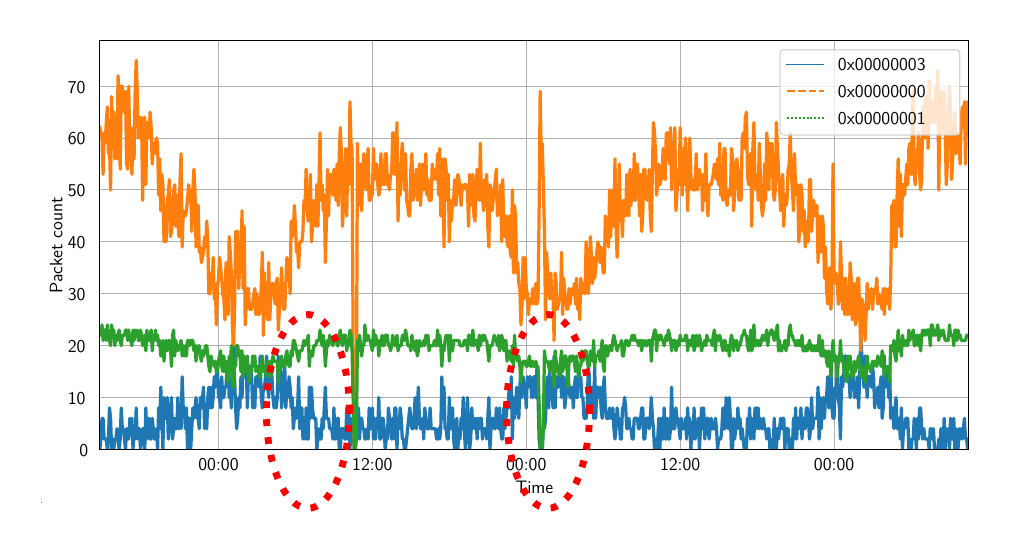
\begin{tikzpicture}
    \node(A){
    \resizebox{0.98\textwidth}{!}
        {
            %% Creator: Matplotlib, PGF backend
%%
%% To include the figure in your LaTeX document, write
%%   \input{<filename>.pgf}
%%
%% Make sure the required packages are loaded in your preamble
%%   \usepackage{pgf}
%%
%% Also ensure that all the required font packages are loaded; for instance,
%% the lmodern package is sometimes necessary when using math font.
%%   \usepackage{lmodern}
%%
%% Figures using additional raster images can only be included by \input if
%% they are in the same directory as the main LaTeX file. For loading figures
%% from other directories you can use the `import` package
%%   \usepackage{import}
%%
%% and then include the figures with
%%   \import{<path to file>}{<filename>.pgf}
%%
%% Matplotlib used the following preamble
%%   \usepackage{fontspec}
%%   \setmainfont{DejaVuSerif.ttf}[Path=\detokenize{/home/ankimme/fit/ibt/env/lib/python3.10/site-packages/matplotlib/mpl-data/fonts/ttf/}]
%%   \setsansfont{DejaVuSans.ttf}[Path=\detokenize{/home/ankimme/fit/ibt/env/lib/python3.10/site-packages/matplotlib/mpl-data/fonts/ttf/}]
%%   \setmonofont{DejaVuSansMono.ttf}[Path=\detokenize{/home/ankimme/fit/ibt/env/lib/python3.10/site-packages/matplotlib/mpl-data/fonts/ttf/}]
%%
\begingroup%
\makeatletter%
\begin{pgfpicture}%
\pgfpathrectangle{\pgfpointorigin}{\pgfqpoint{10.000000in}{5.000000in}}%
\pgfusepath{use as bounding box, clip}%
\begin{pgfscope}%
\pgfsetbuttcap%
\pgfsetmiterjoin%
\pgfsetlinewidth{0.000000pt}%
\definecolor{currentstroke}{rgb}{1.000000,1.000000,1.000000}%
\pgfsetstrokecolor{currentstroke}%
\pgfsetstrokeopacity{0.000000}%
\pgfsetdash{}{0pt}%
\pgfpathmoveto{\pgfqpoint{0.000000in}{0.000000in}}%
\pgfpathlineto{\pgfqpoint{10.000000in}{0.000000in}}%
\pgfpathlineto{\pgfqpoint{10.000000in}{5.000000in}}%
\pgfpathlineto{\pgfqpoint{0.000000in}{5.000000in}}%
\pgfpathlineto{\pgfqpoint{0.000000in}{0.000000in}}%
\pgfpathclose%
\pgfusepath{}%
\end{pgfscope}%
\begin{pgfscope}%
\pgfsetbuttcap%
\pgfsetmiterjoin%
\definecolor{currentfill}{rgb}{1.000000,1.000000,1.000000}%
\pgfsetfillcolor{currentfill}%
\pgfsetlinewidth{0.000000pt}%
\definecolor{currentstroke}{rgb}{0.000000,0.000000,0.000000}%
\pgfsetstrokecolor{currentstroke}%
\pgfsetstrokeopacity{0.000000}%
\pgfsetdash{}{0pt}%
\pgfpathmoveto{\pgfqpoint{0.630049in}{0.570804in}}%
\pgfpathlineto{\pgfqpoint{9.958330in}{0.570804in}}%
\pgfpathlineto{\pgfqpoint{9.958330in}{4.958330in}}%
\pgfpathlineto{\pgfqpoint{0.630049in}{4.958330in}}%
\pgfpathlineto{\pgfqpoint{0.630049in}{0.570804in}}%
\pgfpathclose%
\pgfusepath{fill}%
\end{pgfscope}%
\begin{pgfscope}%
\pgfpathrectangle{\pgfqpoint{0.630049in}{0.570804in}}{\pgfqpoint{9.328281in}{4.387526in}}%
\pgfusepath{clip}%
\pgfsetrectcap%
\pgfsetroundjoin%
\pgfsetlinewidth{0.803000pt}%
\definecolor{currentstroke}{rgb}{0.690196,0.690196,0.690196}%
\pgfsetstrokecolor{currentstroke}%
\pgfsetdash{}{0pt}%
\pgfpathmoveto{\pgfqpoint{1.903652in}{0.570804in}}%
\pgfpathlineto{\pgfqpoint{1.903652in}{4.958330in}}%
\pgfusepath{stroke}%
\end{pgfscope}%
\begin{pgfscope}%
\pgfsetbuttcap%
\pgfsetroundjoin%
\definecolor{currentfill}{rgb}{0.000000,0.000000,0.000000}%
\pgfsetfillcolor{currentfill}%
\pgfsetlinewidth{0.803000pt}%
\definecolor{currentstroke}{rgb}{0.000000,0.000000,0.000000}%
\pgfsetstrokecolor{currentstroke}%
\pgfsetdash{}{0pt}%
\pgfsys@defobject{currentmarker}{\pgfqpoint{0.000000in}{-0.048611in}}{\pgfqpoint{0.000000in}{0.000000in}}{%
\pgfpathmoveto{\pgfqpoint{0.000000in}{0.000000in}}%
\pgfpathlineto{\pgfqpoint{0.000000in}{-0.048611in}}%
\pgfusepath{stroke,fill}%
}%
\begin{pgfscope}%
\pgfsys@transformshift{1.903652in}{0.570804in}%
\pgfsys@useobject{currentmarker}{}%
\end{pgfscope}%
\end{pgfscope}%
\begin{pgfscope}%
\definecolor{textcolor}{rgb}{0.000000,0.000000,0.000000}%
\pgfsetstrokecolor{textcolor}%
\pgfsetfillcolor{textcolor}%
\pgftext[x=1.903652in,y=0.473582in,,top]{\color{textcolor}\sffamily\fontsize{14.000000}{16.800000}\selectfont 00:00}%
\end{pgfscope}%
\begin{pgfscope}%
\pgfpathrectangle{\pgfqpoint{0.630049in}{0.570804in}}{\pgfqpoint{9.328281in}{4.387526in}}%
\pgfusepath{clip}%
\pgfsetrectcap%
\pgfsetroundjoin%
\pgfsetlinewidth{0.803000pt}%
\definecolor{currentstroke}{rgb}{0.690196,0.690196,0.690196}%
\pgfsetstrokecolor{currentstroke}%
\pgfsetdash{}{0pt}%
\pgfpathmoveto{\pgfqpoint{3.555893in}{0.570804in}}%
\pgfpathlineto{\pgfqpoint{3.555893in}{4.958330in}}%
\pgfusepath{stroke}%
\end{pgfscope}%
\begin{pgfscope}%
\pgfsetbuttcap%
\pgfsetroundjoin%
\definecolor{currentfill}{rgb}{0.000000,0.000000,0.000000}%
\pgfsetfillcolor{currentfill}%
\pgfsetlinewidth{0.803000pt}%
\definecolor{currentstroke}{rgb}{0.000000,0.000000,0.000000}%
\pgfsetstrokecolor{currentstroke}%
\pgfsetdash{}{0pt}%
\pgfsys@defobject{currentmarker}{\pgfqpoint{0.000000in}{-0.048611in}}{\pgfqpoint{0.000000in}{0.000000in}}{%
\pgfpathmoveto{\pgfqpoint{0.000000in}{0.000000in}}%
\pgfpathlineto{\pgfqpoint{0.000000in}{-0.048611in}}%
\pgfusepath{stroke,fill}%
}%
\begin{pgfscope}%
\pgfsys@transformshift{3.555893in}{0.570804in}%
\pgfsys@useobject{currentmarker}{}%
\end{pgfscope}%
\end{pgfscope}%
\begin{pgfscope}%
\definecolor{textcolor}{rgb}{0.000000,0.000000,0.000000}%
\pgfsetstrokecolor{textcolor}%
\pgfsetfillcolor{textcolor}%
\pgftext[x=3.555893in,y=0.473582in,,top]{\color{textcolor}\sffamily\fontsize{14.000000}{16.800000}\selectfont 12:00}%
\end{pgfscope}%
\begin{pgfscope}%
\pgfpathrectangle{\pgfqpoint{0.630049in}{0.570804in}}{\pgfqpoint{9.328281in}{4.387526in}}%
\pgfusepath{clip}%
\pgfsetrectcap%
\pgfsetroundjoin%
\pgfsetlinewidth{0.803000pt}%
\definecolor{currentstroke}{rgb}{0.690196,0.690196,0.690196}%
\pgfsetstrokecolor{currentstroke}%
\pgfsetdash{}{0pt}%
\pgfpathmoveto{\pgfqpoint{5.208135in}{0.570804in}}%
\pgfpathlineto{\pgfqpoint{5.208135in}{4.958330in}}%
\pgfusepath{stroke}%
\end{pgfscope}%
\begin{pgfscope}%
\pgfsetbuttcap%
\pgfsetroundjoin%
\definecolor{currentfill}{rgb}{0.000000,0.000000,0.000000}%
\pgfsetfillcolor{currentfill}%
\pgfsetlinewidth{0.803000pt}%
\definecolor{currentstroke}{rgb}{0.000000,0.000000,0.000000}%
\pgfsetstrokecolor{currentstroke}%
\pgfsetdash{}{0pt}%
\pgfsys@defobject{currentmarker}{\pgfqpoint{0.000000in}{-0.048611in}}{\pgfqpoint{0.000000in}{0.000000in}}{%
\pgfpathmoveto{\pgfqpoint{0.000000in}{0.000000in}}%
\pgfpathlineto{\pgfqpoint{0.000000in}{-0.048611in}}%
\pgfusepath{stroke,fill}%
}%
\begin{pgfscope}%
\pgfsys@transformshift{5.208135in}{0.570804in}%
\pgfsys@useobject{currentmarker}{}%
\end{pgfscope}%
\end{pgfscope}%
\begin{pgfscope}%
\definecolor{textcolor}{rgb}{0.000000,0.000000,0.000000}%
\pgfsetstrokecolor{textcolor}%
\pgfsetfillcolor{textcolor}%
\pgftext[x=5.208135in,y=0.473582in,,top]{\color{textcolor}\sffamily\fontsize{14.000000}{16.800000}\selectfont 00:00}%
\end{pgfscope}%
\begin{pgfscope}%
\pgfpathrectangle{\pgfqpoint{0.630049in}{0.570804in}}{\pgfqpoint{9.328281in}{4.387526in}}%
\pgfusepath{clip}%
\pgfsetrectcap%
\pgfsetroundjoin%
\pgfsetlinewidth{0.803000pt}%
\definecolor{currentstroke}{rgb}{0.690196,0.690196,0.690196}%
\pgfsetstrokecolor{currentstroke}%
\pgfsetdash{}{0pt}%
\pgfpathmoveto{\pgfqpoint{6.860377in}{0.570804in}}%
\pgfpathlineto{\pgfqpoint{6.860377in}{4.958330in}}%
\pgfusepath{stroke}%
\end{pgfscope}%
\begin{pgfscope}%
\pgfsetbuttcap%
\pgfsetroundjoin%
\definecolor{currentfill}{rgb}{0.000000,0.000000,0.000000}%
\pgfsetfillcolor{currentfill}%
\pgfsetlinewidth{0.803000pt}%
\definecolor{currentstroke}{rgb}{0.000000,0.000000,0.000000}%
\pgfsetstrokecolor{currentstroke}%
\pgfsetdash{}{0pt}%
\pgfsys@defobject{currentmarker}{\pgfqpoint{0.000000in}{-0.048611in}}{\pgfqpoint{0.000000in}{0.000000in}}{%
\pgfpathmoveto{\pgfqpoint{0.000000in}{0.000000in}}%
\pgfpathlineto{\pgfqpoint{0.000000in}{-0.048611in}}%
\pgfusepath{stroke,fill}%
}%
\begin{pgfscope}%
\pgfsys@transformshift{6.860377in}{0.570804in}%
\pgfsys@useobject{currentmarker}{}%
\end{pgfscope}%
\end{pgfscope}%
\begin{pgfscope}%
\definecolor{textcolor}{rgb}{0.000000,0.000000,0.000000}%
\pgfsetstrokecolor{textcolor}%
\pgfsetfillcolor{textcolor}%
\pgftext[x=6.860377in,y=0.473582in,,top]{\color{textcolor}\sffamily\fontsize{14.000000}{16.800000}\selectfont 12:00}%
\end{pgfscope}%
\begin{pgfscope}%
\pgfpathrectangle{\pgfqpoint{0.630049in}{0.570804in}}{\pgfqpoint{9.328281in}{4.387526in}}%
\pgfusepath{clip}%
\pgfsetrectcap%
\pgfsetroundjoin%
\pgfsetlinewidth{0.803000pt}%
\definecolor{currentstroke}{rgb}{0.690196,0.690196,0.690196}%
\pgfsetstrokecolor{currentstroke}%
\pgfsetdash{}{0pt}%
\pgfpathmoveto{\pgfqpoint{8.512619in}{0.570804in}}%
\pgfpathlineto{\pgfqpoint{8.512619in}{4.958330in}}%
\pgfusepath{stroke}%
\end{pgfscope}%
\begin{pgfscope}%
\pgfsetbuttcap%
\pgfsetroundjoin%
\definecolor{currentfill}{rgb}{0.000000,0.000000,0.000000}%
\pgfsetfillcolor{currentfill}%
\pgfsetlinewidth{0.803000pt}%
\definecolor{currentstroke}{rgb}{0.000000,0.000000,0.000000}%
\pgfsetstrokecolor{currentstroke}%
\pgfsetdash{}{0pt}%
\pgfsys@defobject{currentmarker}{\pgfqpoint{0.000000in}{-0.048611in}}{\pgfqpoint{0.000000in}{0.000000in}}{%
\pgfpathmoveto{\pgfqpoint{0.000000in}{0.000000in}}%
\pgfpathlineto{\pgfqpoint{0.000000in}{-0.048611in}}%
\pgfusepath{stroke,fill}%
}%
\begin{pgfscope}%
\pgfsys@transformshift{8.512619in}{0.570804in}%
\pgfsys@useobject{currentmarker}{}%
\end{pgfscope}%
\end{pgfscope}%
\begin{pgfscope}%
\definecolor{textcolor}{rgb}{0.000000,0.000000,0.000000}%
\pgfsetstrokecolor{textcolor}%
\pgfsetfillcolor{textcolor}%
\pgftext[x=8.512619in,y=0.473582in,,top]{\color{textcolor}\sffamily\fontsize{14.000000}{16.800000}\selectfont 00:00}%
\end{pgfscope}%
\begin{pgfscope}%
\definecolor{textcolor}{rgb}{0.000000,0.000000,0.000000}%
\pgfsetstrokecolor{textcolor}%
\pgfsetfillcolor{textcolor}%
\pgftext[x=5.294189in,y=0.229848in,,top]{\color{textcolor}\sffamily\fontsize{14.000000}{16.800000}\selectfont Time}%
\end{pgfscope}%
\begin{pgfscope}%
\pgfpathrectangle{\pgfqpoint{0.630049in}{0.570804in}}{\pgfqpoint{9.328281in}{4.387526in}}%
\pgfusepath{clip}%
\pgfsetrectcap%
\pgfsetroundjoin%
\pgfsetlinewidth{0.803000pt}%
\definecolor{currentstroke}{rgb}{0.690196,0.690196,0.690196}%
\pgfsetstrokecolor{currentstroke}%
\pgfsetdash{}{0pt}%
\pgfpathmoveto{\pgfqpoint{0.630049in}{0.570804in}}%
\pgfpathlineto{\pgfqpoint{9.958330in}{0.570804in}}%
\pgfusepath{stroke}%
\end{pgfscope}%
\begin{pgfscope}%
\pgfsetbuttcap%
\pgfsetroundjoin%
\definecolor{currentfill}{rgb}{0.000000,0.000000,0.000000}%
\pgfsetfillcolor{currentfill}%
\pgfsetlinewidth{0.803000pt}%
\definecolor{currentstroke}{rgb}{0.000000,0.000000,0.000000}%
\pgfsetstrokecolor{currentstroke}%
\pgfsetdash{}{0pt}%
\pgfsys@defobject{currentmarker}{\pgfqpoint{-0.048611in}{0.000000in}}{\pgfqpoint{-0.000000in}{0.000000in}}{%
\pgfpathmoveto{\pgfqpoint{-0.000000in}{0.000000in}}%
\pgfpathlineto{\pgfqpoint{-0.048611in}{0.000000in}}%
\pgfusepath{stroke,fill}%
}%
\begin{pgfscope}%
\pgfsys@transformshift{0.630049in}{0.570804in}%
\pgfsys@useobject{currentmarker}{}%
\end{pgfscope}%
\end{pgfscope}%
\begin{pgfscope}%
\definecolor{textcolor}{rgb}{0.000000,0.000000,0.000000}%
\pgfsetstrokecolor{textcolor}%
\pgfsetfillcolor{textcolor}%
\pgftext[x=0.409115in, y=0.496938in, left, base]{\color{textcolor}\sffamily\fontsize{14.000000}{16.800000}\selectfont 0}%
\end{pgfscope}%
\begin{pgfscope}%
\pgfpathrectangle{\pgfqpoint{0.630049in}{0.570804in}}{\pgfqpoint{9.328281in}{4.387526in}}%
\pgfusepath{clip}%
\pgfsetrectcap%
\pgfsetroundjoin%
\pgfsetlinewidth{0.803000pt}%
\definecolor{currentstroke}{rgb}{0.690196,0.690196,0.690196}%
\pgfsetstrokecolor{currentstroke}%
\pgfsetdash{}{0pt}%
\pgfpathmoveto{\pgfqpoint{0.630049in}{1.127950in}}%
\pgfpathlineto{\pgfqpoint{9.958330in}{1.127950in}}%
\pgfusepath{stroke}%
\end{pgfscope}%
\begin{pgfscope}%
\pgfsetbuttcap%
\pgfsetroundjoin%
\definecolor{currentfill}{rgb}{0.000000,0.000000,0.000000}%
\pgfsetfillcolor{currentfill}%
\pgfsetlinewidth{0.803000pt}%
\definecolor{currentstroke}{rgb}{0.000000,0.000000,0.000000}%
\pgfsetstrokecolor{currentstroke}%
\pgfsetdash{}{0pt}%
\pgfsys@defobject{currentmarker}{\pgfqpoint{-0.048611in}{0.000000in}}{\pgfqpoint{-0.000000in}{0.000000in}}{%
\pgfpathmoveto{\pgfqpoint{-0.000000in}{0.000000in}}%
\pgfpathlineto{\pgfqpoint{-0.048611in}{0.000000in}}%
\pgfusepath{stroke,fill}%
}%
\begin{pgfscope}%
\pgfsys@transformshift{0.630049in}{1.127950in}%
\pgfsys@useobject{currentmarker}{}%
\end{pgfscope}%
\end{pgfscope}%
\begin{pgfscope}%
\definecolor{textcolor}{rgb}{0.000000,0.000000,0.000000}%
\pgfsetstrokecolor{textcolor}%
\pgfsetfillcolor{textcolor}%
\pgftext[x=0.285404in, y=1.054084in, left, base]{\color{textcolor}\sffamily\fontsize{14.000000}{16.800000}\selectfont 10}%
\end{pgfscope}%
\begin{pgfscope}%
\pgfpathrectangle{\pgfqpoint{0.630049in}{0.570804in}}{\pgfqpoint{9.328281in}{4.387526in}}%
\pgfusepath{clip}%
\pgfsetrectcap%
\pgfsetroundjoin%
\pgfsetlinewidth{0.803000pt}%
\definecolor{currentstroke}{rgb}{0.690196,0.690196,0.690196}%
\pgfsetstrokecolor{currentstroke}%
\pgfsetdash{}{0pt}%
\pgfpathmoveto{\pgfqpoint{0.630049in}{1.685096in}}%
\pgfpathlineto{\pgfqpoint{9.958330in}{1.685096in}}%
\pgfusepath{stroke}%
\end{pgfscope}%
\begin{pgfscope}%
\pgfsetbuttcap%
\pgfsetroundjoin%
\definecolor{currentfill}{rgb}{0.000000,0.000000,0.000000}%
\pgfsetfillcolor{currentfill}%
\pgfsetlinewidth{0.803000pt}%
\definecolor{currentstroke}{rgb}{0.000000,0.000000,0.000000}%
\pgfsetstrokecolor{currentstroke}%
\pgfsetdash{}{0pt}%
\pgfsys@defobject{currentmarker}{\pgfqpoint{-0.048611in}{0.000000in}}{\pgfqpoint{-0.000000in}{0.000000in}}{%
\pgfpathmoveto{\pgfqpoint{-0.000000in}{0.000000in}}%
\pgfpathlineto{\pgfqpoint{-0.048611in}{0.000000in}}%
\pgfusepath{stroke,fill}%
}%
\begin{pgfscope}%
\pgfsys@transformshift{0.630049in}{1.685096in}%
\pgfsys@useobject{currentmarker}{}%
\end{pgfscope}%
\end{pgfscope}%
\begin{pgfscope}%
\definecolor{textcolor}{rgb}{0.000000,0.000000,0.000000}%
\pgfsetstrokecolor{textcolor}%
\pgfsetfillcolor{textcolor}%
\pgftext[x=0.285404in, y=1.611230in, left, base]{\color{textcolor}\sffamily\fontsize{14.000000}{16.800000}\selectfont 20}%
\end{pgfscope}%
\begin{pgfscope}%
\pgfpathrectangle{\pgfqpoint{0.630049in}{0.570804in}}{\pgfqpoint{9.328281in}{4.387526in}}%
\pgfusepath{clip}%
\pgfsetrectcap%
\pgfsetroundjoin%
\pgfsetlinewidth{0.803000pt}%
\definecolor{currentstroke}{rgb}{0.690196,0.690196,0.690196}%
\pgfsetstrokecolor{currentstroke}%
\pgfsetdash{}{0pt}%
\pgfpathmoveto{\pgfqpoint{0.630049in}{2.242242in}}%
\pgfpathlineto{\pgfqpoint{9.958330in}{2.242242in}}%
\pgfusepath{stroke}%
\end{pgfscope}%
\begin{pgfscope}%
\pgfsetbuttcap%
\pgfsetroundjoin%
\definecolor{currentfill}{rgb}{0.000000,0.000000,0.000000}%
\pgfsetfillcolor{currentfill}%
\pgfsetlinewidth{0.803000pt}%
\definecolor{currentstroke}{rgb}{0.000000,0.000000,0.000000}%
\pgfsetstrokecolor{currentstroke}%
\pgfsetdash{}{0pt}%
\pgfsys@defobject{currentmarker}{\pgfqpoint{-0.048611in}{0.000000in}}{\pgfqpoint{-0.000000in}{0.000000in}}{%
\pgfpathmoveto{\pgfqpoint{-0.000000in}{0.000000in}}%
\pgfpathlineto{\pgfqpoint{-0.048611in}{0.000000in}}%
\pgfusepath{stroke,fill}%
}%
\begin{pgfscope}%
\pgfsys@transformshift{0.630049in}{2.242242in}%
\pgfsys@useobject{currentmarker}{}%
\end{pgfscope}%
\end{pgfscope}%
\begin{pgfscope}%
\definecolor{textcolor}{rgb}{0.000000,0.000000,0.000000}%
\pgfsetstrokecolor{textcolor}%
\pgfsetfillcolor{textcolor}%
\pgftext[x=0.285404in, y=2.168376in, left, base]{\color{textcolor}\sffamily\fontsize{14.000000}{16.800000}\selectfont 30}%
\end{pgfscope}%
\begin{pgfscope}%
\pgfpathrectangle{\pgfqpoint{0.630049in}{0.570804in}}{\pgfqpoint{9.328281in}{4.387526in}}%
\pgfusepath{clip}%
\pgfsetrectcap%
\pgfsetroundjoin%
\pgfsetlinewidth{0.803000pt}%
\definecolor{currentstroke}{rgb}{0.690196,0.690196,0.690196}%
\pgfsetstrokecolor{currentstroke}%
\pgfsetdash{}{0pt}%
\pgfpathmoveto{\pgfqpoint{0.630049in}{2.799389in}}%
\pgfpathlineto{\pgfqpoint{9.958330in}{2.799389in}}%
\pgfusepath{stroke}%
\end{pgfscope}%
\begin{pgfscope}%
\pgfsetbuttcap%
\pgfsetroundjoin%
\definecolor{currentfill}{rgb}{0.000000,0.000000,0.000000}%
\pgfsetfillcolor{currentfill}%
\pgfsetlinewidth{0.803000pt}%
\definecolor{currentstroke}{rgb}{0.000000,0.000000,0.000000}%
\pgfsetstrokecolor{currentstroke}%
\pgfsetdash{}{0pt}%
\pgfsys@defobject{currentmarker}{\pgfqpoint{-0.048611in}{0.000000in}}{\pgfqpoint{-0.000000in}{0.000000in}}{%
\pgfpathmoveto{\pgfqpoint{-0.000000in}{0.000000in}}%
\pgfpathlineto{\pgfqpoint{-0.048611in}{0.000000in}}%
\pgfusepath{stroke,fill}%
}%
\begin{pgfscope}%
\pgfsys@transformshift{0.630049in}{2.799389in}%
\pgfsys@useobject{currentmarker}{}%
\end{pgfscope}%
\end{pgfscope}%
\begin{pgfscope}%
\definecolor{textcolor}{rgb}{0.000000,0.000000,0.000000}%
\pgfsetstrokecolor{textcolor}%
\pgfsetfillcolor{textcolor}%
\pgftext[x=0.285404in, y=2.725522in, left, base]{\color{textcolor}\sffamily\fontsize{14.000000}{16.800000}\selectfont 40}%
\end{pgfscope}%
\begin{pgfscope}%
\pgfpathrectangle{\pgfqpoint{0.630049in}{0.570804in}}{\pgfqpoint{9.328281in}{4.387526in}}%
\pgfusepath{clip}%
\pgfsetrectcap%
\pgfsetroundjoin%
\pgfsetlinewidth{0.803000pt}%
\definecolor{currentstroke}{rgb}{0.690196,0.690196,0.690196}%
\pgfsetstrokecolor{currentstroke}%
\pgfsetdash{}{0pt}%
\pgfpathmoveto{\pgfqpoint{0.630049in}{3.356535in}}%
\pgfpathlineto{\pgfqpoint{9.958330in}{3.356535in}}%
\pgfusepath{stroke}%
\end{pgfscope}%
\begin{pgfscope}%
\pgfsetbuttcap%
\pgfsetroundjoin%
\definecolor{currentfill}{rgb}{0.000000,0.000000,0.000000}%
\pgfsetfillcolor{currentfill}%
\pgfsetlinewidth{0.803000pt}%
\definecolor{currentstroke}{rgb}{0.000000,0.000000,0.000000}%
\pgfsetstrokecolor{currentstroke}%
\pgfsetdash{}{0pt}%
\pgfsys@defobject{currentmarker}{\pgfqpoint{-0.048611in}{0.000000in}}{\pgfqpoint{-0.000000in}{0.000000in}}{%
\pgfpathmoveto{\pgfqpoint{-0.000000in}{0.000000in}}%
\pgfpathlineto{\pgfqpoint{-0.048611in}{0.000000in}}%
\pgfusepath{stroke,fill}%
}%
\begin{pgfscope}%
\pgfsys@transformshift{0.630049in}{3.356535in}%
\pgfsys@useobject{currentmarker}{}%
\end{pgfscope}%
\end{pgfscope}%
\begin{pgfscope}%
\definecolor{textcolor}{rgb}{0.000000,0.000000,0.000000}%
\pgfsetstrokecolor{textcolor}%
\pgfsetfillcolor{textcolor}%
\pgftext[x=0.285404in, y=3.282669in, left, base]{\color{textcolor}\sffamily\fontsize{14.000000}{16.800000}\selectfont 50}%
\end{pgfscope}%
\begin{pgfscope}%
\pgfpathrectangle{\pgfqpoint{0.630049in}{0.570804in}}{\pgfqpoint{9.328281in}{4.387526in}}%
\pgfusepath{clip}%
\pgfsetrectcap%
\pgfsetroundjoin%
\pgfsetlinewidth{0.803000pt}%
\definecolor{currentstroke}{rgb}{0.690196,0.690196,0.690196}%
\pgfsetstrokecolor{currentstroke}%
\pgfsetdash{}{0pt}%
\pgfpathmoveto{\pgfqpoint{0.630049in}{3.913681in}}%
\pgfpathlineto{\pgfqpoint{9.958330in}{3.913681in}}%
\pgfusepath{stroke}%
\end{pgfscope}%
\begin{pgfscope}%
\pgfsetbuttcap%
\pgfsetroundjoin%
\definecolor{currentfill}{rgb}{0.000000,0.000000,0.000000}%
\pgfsetfillcolor{currentfill}%
\pgfsetlinewidth{0.803000pt}%
\definecolor{currentstroke}{rgb}{0.000000,0.000000,0.000000}%
\pgfsetstrokecolor{currentstroke}%
\pgfsetdash{}{0pt}%
\pgfsys@defobject{currentmarker}{\pgfqpoint{-0.048611in}{0.000000in}}{\pgfqpoint{-0.000000in}{0.000000in}}{%
\pgfpathmoveto{\pgfqpoint{-0.000000in}{0.000000in}}%
\pgfpathlineto{\pgfqpoint{-0.048611in}{0.000000in}}%
\pgfusepath{stroke,fill}%
}%
\begin{pgfscope}%
\pgfsys@transformshift{0.630049in}{3.913681in}%
\pgfsys@useobject{currentmarker}{}%
\end{pgfscope}%
\end{pgfscope}%
\begin{pgfscope}%
\definecolor{textcolor}{rgb}{0.000000,0.000000,0.000000}%
\pgfsetstrokecolor{textcolor}%
\pgfsetfillcolor{textcolor}%
\pgftext[x=0.285404in, y=3.839815in, left, base]{\color{textcolor}\sffamily\fontsize{14.000000}{16.800000}\selectfont 60}%
\end{pgfscope}%
\begin{pgfscope}%
\pgfpathrectangle{\pgfqpoint{0.630049in}{0.570804in}}{\pgfqpoint{9.328281in}{4.387526in}}%
\pgfusepath{clip}%
\pgfsetrectcap%
\pgfsetroundjoin%
\pgfsetlinewidth{0.803000pt}%
\definecolor{currentstroke}{rgb}{0.690196,0.690196,0.690196}%
\pgfsetstrokecolor{currentstroke}%
\pgfsetdash{}{0pt}%
\pgfpathmoveto{\pgfqpoint{0.630049in}{4.470827in}}%
\pgfpathlineto{\pgfqpoint{9.958330in}{4.470827in}}%
\pgfusepath{stroke}%
\end{pgfscope}%
\begin{pgfscope}%
\pgfsetbuttcap%
\pgfsetroundjoin%
\definecolor{currentfill}{rgb}{0.000000,0.000000,0.000000}%
\pgfsetfillcolor{currentfill}%
\pgfsetlinewidth{0.803000pt}%
\definecolor{currentstroke}{rgb}{0.000000,0.000000,0.000000}%
\pgfsetstrokecolor{currentstroke}%
\pgfsetdash{}{0pt}%
\pgfsys@defobject{currentmarker}{\pgfqpoint{-0.048611in}{0.000000in}}{\pgfqpoint{-0.000000in}{0.000000in}}{%
\pgfpathmoveto{\pgfqpoint{-0.000000in}{0.000000in}}%
\pgfpathlineto{\pgfqpoint{-0.048611in}{0.000000in}}%
\pgfusepath{stroke,fill}%
}%
\begin{pgfscope}%
\pgfsys@transformshift{0.630049in}{4.470827in}%
\pgfsys@useobject{currentmarker}{}%
\end{pgfscope}%
\end{pgfscope}%
\begin{pgfscope}%
\definecolor{textcolor}{rgb}{0.000000,0.000000,0.000000}%
\pgfsetstrokecolor{textcolor}%
\pgfsetfillcolor{textcolor}%
\pgftext[x=0.285404in, y=4.396961in, left, base]{\color{textcolor}\sffamily\fontsize{14.000000}{16.800000}\selectfont 70}%
\end{pgfscope}%
\begin{pgfscope}%
\definecolor{textcolor}{rgb}{0.000000,0.000000,0.000000}%
\pgfsetstrokecolor{textcolor}%
\pgfsetfillcolor{textcolor}%
\pgftext[x=0.229848in,y=2.764567in,,bottom,rotate=90.000000]{\color{textcolor}\sffamily\fontsize{14.000000}{16.800000}\selectfont Packet count}%
\end{pgfscope}%
\begin{pgfscope}%
\pgfpathrectangle{\pgfqpoint{0.630049in}{0.570804in}}{\pgfqpoint{9.328281in}{4.387526in}}%
\pgfusepath{clip}%
\pgfsetrectcap%
\pgfsetroundjoin%
\pgfsetlinewidth{2.509375pt}%
\definecolor{currentstroke}{rgb}{0.121569,0.466667,0.705882}%
\pgfsetstrokecolor{currentstroke}%
\pgfsetdash{}{0pt}%
\pgfpathmoveto{\pgfqpoint{0.630049in}{0.570804in}}%
\pgfpathlineto{\pgfqpoint{0.641523in}{0.682233in}}%
\pgfpathlineto{\pgfqpoint{0.652997in}{0.905092in}}%
\pgfpathlineto{\pgfqpoint{0.664470in}{0.905092in}}%
\pgfpathlineto{\pgfqpoint{0.675944in}{0.682233in}}%
\pgfpathlineto{\pgfqpoint{0.698892in}{0.682233in}}%
\pgfpathlineto{\pgfqpoint{0.710366in}{0.570804in}}%
\pgfpathlineto{\pgfqpoint{0.721840in}{0.682233in}}%
\pgfpathlineto{\pgfqpoint{0.733314in}{1.016521in}}%
\pgfpathlineto{\pgfqpoint{0.744788in}{0.905092in}}%
\pgfpathlineto{\pgfqpoint{0.756262in}{0.570804in}}%
\pgfpathlineto{\pgfqpoint{0.767736in}{0.682233in}}%
\pgfpathlineto{\pgfqpoint{0.779209in}{0.570804in}}%
\pgfpathlineto{\pgfqpoint{0.790683in}{0.682233in}}%
\pgfpathlineto{\pgfqpoint{0.802157in}{0.682233in}}%
\pgfpathlineto{\pgfqpoint{0.813631in}{0.793662in}}%
\pgfpathlineto{\pgfqpoint{0.836579in}{0.570804in}}%
\pgfpathlineto{\pgfqpoint{0.848053in}{0.682233in}}%
\pgfpathlineto{\pgfqpoint{0.859527in}{1.016521in}}%
\pgfpathlineto{\pgfqpoint{0.871001in}{0.793662in}}%
\pgfpathlineto{\pgfqpoint{0.882475in}{0.793662in}}%
\pgfpathlineto{\pgfqpoint{0.905422in}{0.570804in}}%
\pgfpathlineto{\pgfqpoint{0.916896in}{0.793662in}}%
\pgfpathlineto{\pgfqpoint{0.928370in}{0.682233in}}%
\pgfpathlineto{\pgfqpoint{0.939844in}{0.682233in}}%
\pgfpathlineto{\pgfqpoint{0.951318in}{0.905092in}}%
\pgfpathlineto{\pgfqpoint{0.962792in}{0.793662in}}%
\pgfpathlineto{\pgfqpoint{0.974266in}{0.905092in}}%
\pgfpathlineto{\pgfqpoint{0.985740in}{0.570804in}}%
\pgfpathlineto{\pgfqpoint{0.997214in}{0.793662in}}%
\pgfpathlineto{\pgfqpoint{1.008687in}{0.682233in}}%
\pgfpathlineto{\pgfqpoint{1.020161in}{1.016521in}}%
\pgfpathlineto{\pgfqpoint{1.031635in}{0.682233in}}%
\pgfpathlineto{\pgfqpoint{1.043109in}{0.793662in}}%
\pgfpathlineto{\pgfqpoint{1.054583in}{0.793662in}}%
\pgfpathlineto{\pgfqpoint{1.066057in}{0.570804in}}%
\pgfpathlineto{\pgfqpoint{1.089005in}{0.793662in}}%
\pgfpathlineto{\pgfqpoint{1.100479in}{0.793662in}}%
\pgfpathlineto{\pgfqpoint{1.111953in}{0.570804in}}%
\pgfpathlineto{\pgfqpoint{1.123426in}{1.016521in}}%
\pgfpathlineto{\pgfqpoint{1.134900in}{0.682233in}}%
\pgfpathlineto{\pgfqpoint{1.157848in}{0.905092in}}%
\pgfpathlineto{\pgfqpoint{1.169322in}{0.682233in}}%
\pgfpathlineto{\pgfqpoint{1.180796in}{0.682233in}}%
\pgfpathlineto{\pgfqpoint{1.192270in}{0.905092in}}%
\pgfpathlineto{\pgfqpoint{1.215218in}{0.682233in}}%
\pgfpathlineto{\pgfqpoint{1.226692in}{0.682233in}}%
\pgfpathlineto{\pgfqpoint{1.238165in}{0.793662in}}%
\pgfpathlineto{\pgfqpoint{1.249639in}{0.570804in}}%
\pgfpathlineto{\pgfqpoint{1.261113in}{1.016521in}}%
\pgfpathlineto{\pgfqpoint{1.272587in}{0.793662in}}%
\pgfpathlineto{\pgfqpoint{1.284061in}{1.239379in}}%
\pgfpathlineto{\pgfqpoint{1.307009in}{0.570804in}}%
\pgfpathlineto{\pgfqpoint{1.318483in}{1.127950in}}%
\pgfpathlineto{\pgfqpoint{1.329957in}{0.905092in}}%
\pgfpathlineto{\pgfqpoint{1.341431in}{0.905092in}}%
\pgfpathlineto{\pgfqpoint{1.352904in}{1.127950in}}%
\pgfpathlineto{\pgfqpoint{1.364378in}{0.682233in}}%
\pgfpathlineto{\pgfqpoint{1.375852in}{0.793662in}}%
\pgfpathlineto{\pgfqpoint{1.387326in}{1.016521in}}%
\pgfpathlineto{\pgfqpoint{1.398800in}{1.127950in}}%
\pgfpathlineto{\pgfqpoint{1.410274in}{0.682233in}}%
\pgfpathlineto{\pgfqpoint{1.433222in}{0.905092in}}%
\pgfpathlineto{\pgfqpoint{1.444696in}{0.793662in}}%
\pgfpathlineto{\pgfqpoint{1.456170in}{0.793662in}}%
\pgfpathlineto{\pgfqpoint{1.467643in}{1.127950in}}%
\pgfpathlineto{\pgfqpoint{1.479117in}{0.793662in}}%
\pgfpathlineto{\pgfqpoint{1.490591in}{1.016521in}}%
\pgfpathlineto{\pgfqpoint{1.502065in}{0.793662in}}%
\pgfpathlineto{\pgfqpoint{1.513539in}{1.350809in}}%
\pgfpathlineto{\pgfqpoint{1.525013in}{1.016521in}}%
\pgfpathlineto{\pgfqpoint{1.536487in}{1.016521in}}%
\pgfpathlineto{\pgfqpoint{1.547961in}{0.793662in}}%
\pgfpathlineto{\pgfqpoint{1.559435in}{1.016521in}}%
\pgfpathlineto{\pgfqpoint{1.570909in}{0.570804in}}%
\pgfpathlineto{\pgfqpoint{1.582383in}{0.905092in}}%
\pgfpathlineto{\pgfqpoint{1.593856in}{0.905092in}}%
\pgfpathlineto{\pgfqpoint{1.605330in}{0.570804in}}%
\pgfpathlineto{\pgfqpoint{1.628278in}{1.016521in}}%
\pgfpathlineto{\pgfqpoint{1.639752in}{0.905092in}}%
\pgfpathlineto{\pgfqpoint{1.662700in}{1.127950in}}%
\pgfpathlineto{\pgfqpoint{1.674174in}{0.905092in}}%
\pgfpathlineto{\pgfqpoint{1.685648in}{0.905092in}}%
\pgfpathlineto{\pgfqpoint{1.697122in}{0.793662in}}%
\pgfpathlineto{\pgfqpoint{1.708595in}{1.127950in}}%
\pgfpathlineto{\pgfqpoint{1.720069in}{1.016521in}}%
\pgfpathlineto{\pgfqpoint{1.743017in}{1.239379in}}%
\pgfpathlineto{\pgfqpoint{1.754491in}{0.793662in}}%
\pgfpathlineto{\pgfqpoint{1.765965in}{0.905092in}}%
\pgfpathlineto{\pgfqpoint{1.777439in}{0.793662in}}%
\pgfpathlineto{\pgfqpoint{1.788913in}{1.127950in}}%
\pgfpathlineto{\pgfqpoint{1.800387in}{1.239379in}}%
\pgfpathlineto{\pgfqpoint{1.811861in}{1.016521in}}%
\pgfpathlineto{\pgfqpoint{1.823334in}{1.239379in}}%
\pgfpathlineto{\pgfqpoint{1.834808in}{1.016521in}}%
\pgfpathlineto{\pgfqpoint{1.846282in}{1.127950in}}%
\pgfpathlineto{\pgfqpoint{1.857756in}{1.350809in}}%
\pgfpathlineto{\pgfqpoint{1.869230in}{1.239379in}}%
\pgfpathlineto{\pgfqpoint{1.892178in}{1.462238in}}%
\pgfpathlineto{\pgfqpoint{1.903652in}{1.127950in}}%
\pgfpathlineto{\pgfqpoint{1.915126in}{1.127950in}}%
\pgfpathlineto{\pgfqpoint{1.926600in}{1.016521in}}%
\pgfpathlineto{\pgfqpoint{1.938073in}{1.350809in}}%
\pgfpathlineto{\pgfqpoint{1.949547in}{1.127950in}}%
\pgfpathlineto{\pgfqpoint{1.961021in}{1.127950in}}%
\pgfpathlineto{\pgfqpoint{1.972495in}{1.239379in}}%
\pgfpathlineto{\pgfqpoint{1.983969in}{1.239379in}}%
\pgfpathlineto{\pgfqpoint{1.995443in}{1.462238in}}%
\pgfpathlineto{\pgfqpoint{2.006917in}{1.462238in}}%
\pgfpathlineto{\pgfqpoint{2.018391in}{1.127950in}}%
\pgfpathlineto{\pgfqpoint{2.029865in}{1.239379in}}%
\pgfpathlineto{\pgfqpoint{2.041339in}{1.016521in}}%
\pgfpathlineto{\pgfqpoint{2.052812in}{1.462238in}}%
\pgfpathlineto{\pgfqpoint{2.064286in}{1.796525in}}%
\pgfpathlineto{\pgfqpoint{2.075760in}{1.350809in}}%
\pgfpathlineto{\pgfqpoint{2.087234in}{1.016521in}}%
\pgfpathlineto{\pgfqpoint{2.098708in}{0.793662in}}%
\pgfpathlineto{\pgfqpoint{2.110182in}{0.905092in}}%
\pgfpathlineto{\pgfqpoint{2.121656in}{1.127950in}}%
\pgfpathlineto{\pgfqpoint{2.133130in}{1.016521in}}%
\pgfpathlineto{\pgfqpoint{2.144604in}{1.350809in}}%
\pgfpathlineto{\pgfqpoint{2.156078in}{1.127950in}}%
\pgfpathlineto{\pgfqpoint{2.167551in}{1.462238in}}%
\pgfpathlineto{\pgfqpoint{2.179025in}{1.350809in}}%
\pgfpathlineto{\pgfqpoint{2.190499in}{1.350809in}}%
\pgfpathlineto{\pgfqpoint{2.201973in}{1.462238in}}%
\pgfpathlineto{\pgfqpoint{2.213447in}{1.016521in}}%
\pgfpathlineto{\pgfqpoint{2.224921in}{1.350809in}}%
\pgfpathlineto{\pgfqpoint{2.236395in}{1.462238in}}%
\pgfpathlineto{\pgfqpoint{2.247869in}{1.462238in}}%
\pgfpathlineto{\pgfqpoint{2.259343in}{1.350809in}}%
\pgfpathlineto{\pgfqpoint{2.270817in}{1.016521in}}%
\pgfpathlineto{\pgfqpoint{2.282290in}{1.127950in}}%
\pgfpathlineto{\pgfqpoint{2.293764in}{1.016521in}}%
\pgfpathlineto{\pgfqpoint{2.305238in}{1.350809in}}%
\pgfpathlineto{\pgfqpoint{2.328186in}{1.350809in}}%
\pgfpathlineto{\pgfqpoint{2.339660in}{1.239379in}}%
\pgfpathlineto{\pgfqpoint{2.351134in}{1.573667in}}%
\pgfpathlineto{\pgfqpoint{2.362608in}{1.127950in}}%
\pgfpathlineto{\pgfqpoint{2.374082in}{1.016521in}}%
\pgfpathlineto{\pgfqpoint{2.385556in}{1.239379in}}%
\pgfpathlineto{\pgfqpoint{2.397029in}{1.239379in}}%
\pgfpathlineto{\pgfqpoint{2.408503in}{1.350809in}}%
\pgfpathlineto{\pgfqpoint{2.419977in}{1.573667in}}%
\pgfpathlineto{\pgfqpoint{2.431451in}{1.239379in}}%
\pgfpathlineto{\pgfqpoint{2.442925in}{1.127950in}}%
\pgfpathlineto{\pgfqpoint{2.454399in}{1.350809in}}%
\pgfpathlineto{\pgfqpoint{2.465873in}{1.462238in}}%
\pgfpathlineto{\pgfqpoint{2.477347in}{1.350809in}}%
\pgfpathlineto{\pgfqpoint{2.488821in}{1.127950in}}%
\pgfpathlineto{\pgfqpoint{2.500295in}{1.016521in}}%
\pgfpathlineto{\pgfqpoint{2.511768in}{1.127950in}}%
\pgfpathlineto{\pgfqpoint{2.523242in}{1.016521in}}%
\pgfpathlineto{\pgfqpoint{2.534716in}{1.127950in}}%
\pgfpathlineto{\pgfqpoint{2.546190in}{1.573667in}}%
\pgfpathlineto{\pgfqpoint{2.557664in}{1.239379in}}%
\pgfpathlineto{\pgfqpoint{2.569138in}{1.462238in}}%
\pgfpathlineto{\pgfqpoint{2.580612in}{1.016521in}}%
\pgfpathlineto{\pgfqpoint{2.592086in}{1.127950in}}%
\pgfpathlineto{\pgfqpoint{2.603560in}{1.350809in}}%
\pgfpathlineto{\pgfqpoint{2.615034in}{1.462238in}}%
\pgfpathlineto{\pgfqpoint{2.626507in}{1.016521in}}%
\pgfpathlineto{\pgfqpoint{2.637981in}{1.239379in}}%
\pgfpathlineto{\pgfqpoint{2.649455in}{1.127950in}}%
\pgfpathlineto{\pgfqpoint{2.660929in}{1.350809in}}%
\pgfpathlineto{\pgfqpoint{2.672403in}{1.239379in}}%
\pgfpathlineto{\pgfqpoint{2.683877in}{1.016521in}}%
\pgfpathlineto{\pgfqpoint{2.695351in}{1.127950in}}%
\pgfpathlineto{\pgfqpoint{2.706825in}{0.793662in}}%
\pgfpathlineto{\pgfqpoint{2.729773in}{1.016521in}}%
\pgfpathlineto{\pgfqpoint{2.741246in}{0.905092in}}%
\pgfpathlineto{\pgfqpoint{2.752720in}{1.016521in}}%
\pgfpathlineto{\pgfqpoint{2.764194in}{1.350809in}}%
\pgfpathlineto{\pgfqpoint{2.775668in}{0.793662in}}%
\pgfpathlineto{\pgfqpoint{2.787142in}{1.016521in}}%
\pgfpathlineto{\pgfqpoint{2.798616in}{1.016521in}}%
\pgfpathlineto{\pgfqpoint{2.810090in}{0.682233in}}%
\pgfpathlineto{\pgfqpoint{2.821564in}{0.905092in}}%
\pgfpathlineto{\pgfqpoint{2.833038in}{0.682233in}}%
\pgfpathlineto{\pgfqpoint{2.844512in}{1.016521in}}%
\pgfpathlineto{\pgfqpoint{2.855985in}{0.682233in}}%
\pgfpathlineto{\pgfqpoint{2.867459in}{0.682233in}}%
\pgfpathlineto{\pgfqpoint{2.878933in}{1.239379in}}%
\pgfpathlineto{\pgfqpoint{2.890407in}{0.905092in}}%
\pgfpathlineto{\pgfqpoint{2.901881in}{1.239379in}}%
\pgfpathlineto{\pgfqpoint{2.913355in}{1.016521in}}%
\pgfpathlineto{\pgfqpoint{2.924829in}{0.905092in}}%
\pgfpathlineto{\pgfqpoint{2.947777in}{0.905092in}}%
\pgfpathlineto{\pgfqpoint{2.959251in}{0.570804in}}%
\pgfpathlineto{\pgfqpoint{2.982198in}{0.793662in}}%
\pgfpathlineto{\pgfqpoint{2.993672in}{0.682233in}}%
\pgfpathlineto{\pgfqpoint{3.005146in}{0.682233in}}%
\pgfpathlineto{\pgfqpoint{3.016620in}{0.905092in}}%
\pgfpathlineto{\pgfqpoint{3.028094in}{0.793662in}}%
\pgfpathlineto{\pgfqpoint{3.051042in}{1.239379in}}%
\pgfpathlineto{\pgfqpoint{3.062516in}{0.905092in}}%
\pgfpathlineto{\pgfqpoint{3.085463in}{0.905092in}}%
\pgfpathlineto{\pgfqpoint{3.096937in}{0.793662in}}%
\pgfpathlineto{\pgfqpoint{3.119885in}{0.793662in}}%
\pgfpathlineto{\pgfqpoint{3.131359in}{0.682233in}}%
\pgfpathlineto{\pgfqpoint{3.142833in}{1.016521in}}%
\pgfpathlineto{\pgfqpoint{3.154307in}{0.682233in}}%
\pgfpathlineto{\pgfqpoint{3.165781in}{0.682233in}}%
\pgfpathlineto{\pgfqpoint{3.177255in}{0.905092in}}%
\pgfpathlineto{\pgfqpoint{3.188729in}{0.905092in}}%
\pgfpathlineto{\pgfqpoint{3.200203in}{0.570804in}}%
\pgfpathlineto{\pgfqpoint{3.211676in}{0.570804in}}%
\pgfpathlineto{\pgfqpoint{3.223150in}{0.793662in}}%
\pgfpathlineto{\pgfqpoint{3.246098in}{0.793662in}}%
\pgfpathlineto{\pgfqpoint{3.257572in}{0.682233in}}%
\pgfpathlineto{\pgfqpoint{3.269046in}{0.682233in}}%
\pgfpathlineto{\pgfqpoint{3.280520in}{1.016521in}}%
\pgfpathlineto{\pgfqpoint{3.291994in}{0.682233in}}%
\pgfpathlineto{\pgfqpoint{3.303468in}{1.016521in}}%
\pgfpathlineto{\pgfqpoint{3.314942in}{0.570804in}}%
\pgfpathlineto{\pgfqpoint{3.326415in}{0.793662in}}%
\pgfpathlineto{\pgfqpoint{3.337889in}{0.905092in}}%
\pgfpathlineto{\pgfqpoint{3.349363in}{0.793662in}}%
\pgfpathlineto{\pgfqpoint{3.360837in}{0.570804in}}%
\pgfpathlineto{\pgfqpoint{3.372311in}{0.570804in}}%
\pgfpathlineto{\pgfqpoint{3.383785in}{0.793662in}}%
\pgfpathlineto{\pgfqpoint{3.395259in}{0.793662in}}%
\pgfpathlineto{\pgfqpoint{3.406733in}{1.016521in}}%
\pgfpathlineto{\pgfqpoint{3.418207in}{0.682233in}}%
\pgfpathlineto{\pgfqpoint{3.429681in}{0.905092in}}%
\pgfpathlineto{\pgfqpoint{3.441154in}{0.905092in}}%
\pgfpathlineto{\pgfqpoint{3.452628in}{0.793662in}}%
\pgfpathlineto{\pgfqpoint{3.464102in}{0.793662in}}%
\pgfpathlineto{\pgfqpoint{3.475576in}{0.682233in}}%
\pgfpathlineto{\pgfqpoint{3.487050in}{0.682233in}}%
\pgfpathlineto{\pgfqpoint{3.498524in}{0.793662in}}%
\pgfpathlineto{\pgfqpoint{3.509998in}{0.682233in}}%
\pgfpathlineto{\pgfqpoint{3.521472in}{1.016521in}}%
\pgfpathlineto{\pgfqpoint{3.532946in}{0.793662in}}%
\pgfpathlineto{\pgfqpoint{3.544420in}{0.793662in}}%
\pgfpathlineto{\pgfqpoint{3.555893in}{1.016521in}}%
\pgfpathlineto{\pgfqpoint{3.567367in}{0.682233in}}%
\pgfpathlineto{\pgfqpoint{3.578841in}{0.905092in}}%
\pgfpathlineto{\pgfqpoint{3.590315in}{0.682233in}}%
\pgfpathlineto{\pgfqpoint{3.601789in}{0.905092in}}%
\pgfpathlineto{\pgfqpoint{3.613263in}{0.793662in}}%
\pgfpathlineto{\pgfqpoint{3.624737in}{1.127950in}}%
\pgfpathlineto{\pgfqpoint{3.636211in}{0.682233in}}%
\pgfpathlineto{\pgfqpoint{3.647685in}{0.682233in}}%
\pgfpathlineto{\pgfqpoint{3.659159in}{0.905092in}}%
\pgfpathlineto{\pgfqpoint{3.670632in}{0.905092in}}%
\pgfpathlineto{\pgfqpoint{3.682106in}{0.793662in}}%
\pgfpathlineto{\pgfqpoint{3.693580in}{0.570804in}}%
\pgfpathlineto{\pgfqpoint{3.705054in}{0.682233in}}%
\pgfpathlineto{\pgfqpoint{3.716528in}{0.682233in}}%
\pgfpathlineto{\pgfqpoint{3.728002in}{1.016521in}}%
\pgfpathlineto{\pgfqpoint{3.762424in}{0.682233in}}%
\pgfpathlineto{\pgfqpoint{3.773898in}{0.905092in}}%
\pgfpathlineto{\pgfqpoint{3.785371in}{0.682233in}}%
\pgfpathlineto{\pgfqpoint{3.796845in}{1.016521in}}%
\pgfpathlineto{\pgfqpoint{3.808319in}{1.016521in}}%
\pgfpathlineto{\pgfqpoint{3.819793in}{0.570804in}}%
\pgfpathlineto{\pgfqpoint{3.831267in}{0.905092in}}%
\pgfpathlineto{\pgfqpoint{3.842741in}{0.793662in}}%
\pgfpathlineto{\pgfqpoint{3.854215in}{1.016521in}}%
\pgfpathlineto{\pgfqpoint{3.865689in}{0.905092in}}%
\pgfpathlineto{\pgfqpoint{3.877163in}{0.682233in}}%
\pgfpathlineto{\pgfqpoint{3.888637in}{0.682233in}}%
\pgfpathlineto{\pgfqpoint{3.900110in}{0.570804in}}%
\pgfpathlineto{\pgfqpoint{3.911584in}{0.570804in}}%
\pgfpathlineto{\pgfqpoint{3.957480in}{1.016521in}}%
\pgfpathlineto{\pgfqpoint{3.980428in}{0.793662in}}%
\pgfpathlineto{\pgfqpoint{3.991902in}{0.793662in}}%
\pgfpathlineto{\pgfqpoint{4.003376in}{0.905092in}}%
\pgfpathlineto{\pgfqpoint{4.014849in}{1.127950in}}%
\pgfpathlineto{\pgfqpoint{4.026323in}{0.793662in}}%
\pgfpathlineto{\pgfqpoint{4.049271in}{1.239379in}}%
\pgfpathlineto{\pgfqpoint{4.060745in}{0.905092in}}%
\pgfpathlineto{\pgfqpoint{4.072219in}{0.793662in}}%
\pgfpathlineto{\pgfqpoint{4.083693in}{0.793662in}}%
\pgfpathlineto{\pgfqpoint{4.095167in}{0.905092in}}%
\pgfpathlineto{\pgfqpoint{4.106641in}{0.682233in}}%
\pgfpathlineto{\pgfqpoint{4.118115in}{1.016521in}}%
\pgfpathlineto{\pgfqpoint{4.141062in}{0.793662in}}%
\pgfpathlineto{\pgfqpoint{4.164010in}{0.793662in}}%
\pgfpathlineto{\pgfqpoint{4.175484in}{1.016521in}}%
\pgfpathlineto{\pgfqpoint{4.186958in}{0.793662in}}%
\pgfpathlineto{\pgfqpoint{4.232854in}{0.793662in}}%
\pgfpathlineto{\pgfqpoint{4.244327in}{0.682233in}}%
\pgfpathlineto{\pgfqpoint{4.255801in}{0.682233in}}%
\pgfpathlineto{\pgfqpoint{4.267275in}{0.793662in}}%
\pgfpathlineto{\pgfqpoint{4.278749in}{0.682233in}}%
\pgfpathlineto{\pgfqpoint{4.290223in}{0.793662in}}%
\pgfpathlineto{\pgfqpoint{4.301697in}{1.350809in}}%
\pgfpathlineto{\pgfqpoint{4.313171in}{0.905092in}}%
\pgfpathlineto{\pgfqpoint{4.324645in}{1.239379in}}%
\pgfpathlineto{\pgfqpoint{4.336119in}{0.793662in}}%
\pgfpathlineto{\pgfqpoint{4.347593in}{0.793662in}}%
\pgfpathlineto{\pgfqpoint{4.359066in}{0.682233in}}%
\pgfpathlineto{\pgfqpoint{4.370540in}{0.682233in}}%
\pgfpathlineto{\pgfqpoint{4.382014in}{1.127950in}}%
\pgfpathlineto{\pgfqpoint{4.393488in}{0.793662in}}%
\pgfpathlineto{\pgfqpoint{4.416436in}{1.016521in}}%
\pgfpathlineto{\pgfqpoint{4.427910in}{0.682233in}}%
\pgfpathlineto{\pgfqpoint{4.439384in}{0.570804in}}%
\pgfpathlineto{\pgfqpoint{4.450858in}{0.793662in}}%
\pgfpathlineto{\pgfqpoint{4.462332in}{0.905092in}}%
\pgfpathlineto{\pgfqpoint{4.473805in}{0.570804in}}%
\pgfpathlineto{\pgfqpoint{4.485279in}{0.793662in}}%
\pgfpathlineto{\pgfqpoint{4.496753in}{0.682233in}}%
\pgfpathlineto{\pgfqpoint{4.508227in}{0.905092in}}%
\pgfpathlineto{\pgfqpoint{4.519701in}{0.793662in}}%
\pgfpathlineto{\pgfqpoint{4.531175in}{1.127950in}}%
\pgfpathlineto{\pgfqpoint{4.542649in}{0.793662in}}%
\pgfpathlineto{\pgfqpoint{4.554123in}{0.570804in}}%
\pgfpathlineto{\pgfqpoint{4.565597in}{0.793662in}}%
\pgfpathlineto{\pgfqpoint{4.577071in}{1.127950in}}%
\pgfpathlineto{\pgfqpoint{4.588544in}{0.793662in}}%
\pgfpathlineto{\pgfqpoint{4.600018in}{0.570804in}}%
\pgfpathlineto{\pgfqpoint{4.611492in}{0.682233in}}%
\pgfpathlineto{\pgfqpoint{4.622966in}{1.016521in}}%
\pgfpathlineto{\pgfqpoint{4.634440in}{0.793662in}}%
\pgfpathlineto{\pgfqpoint{4.645914in}{0.905092in}}%
\pgfpathlineto{\pgfqpoint{4.657388in}{0.793662in}}%
\pgfpathlineto{\pgfqpoint{4.668862in}{0.905092in}}%
\pgfpathlineto{\pgfqpoint{4.680336in}{0.682233in}}%
\pgfpathlineto{\pgfqpoint{4.691810in}{0.905092in}}%
\pgfpathlineto{\pgfqpoint{4.703283in}{0.793662in}}%
\pgfpathlineto{\pgfqpoint{4.714757in}{0.905092in}}%
\pgfpathlineto{\pgfqpoint{4.726231in}{0.905092in}}%
\pgfpathlineto{\pgfqpoint{4.737705in}{0.682233in}}%
\pgfpathlineto{\pgfqpoint{4.749179in}{0.793662in}}%
\pgfpathlineto{\pgfqpoint{4.772127in}{0.793662in}}%
\pgfpathlineto{\pgfqpoint{4.783601in}{0.682233in}}%
\pgfpathlineto{\pgfqpoint{4.806549in}{1.127950in}}%
\pgfpathlineto{\pgfqpoint{4.818022in}{0.570804in}}%
\pgfpathlineto{\pgfqpoint{4.829496in}{0.793662in}}%
\pgfpathlineto{\pgfqpoint{4.840970in}{0.905092in}}%
\pgfpathlineto{\pgfqpoint{4.852444in}{0.905092in}}%
\pgfpathlineto{\pgfqpoint{4.863918in}{0.793662in}}%
\pgfpathlineto{\pgfqpoint{4.875392in}{0.793662in}}%
\pgfpathlineto{\pgfqpoint{4.886866in}{1.016521in}}%
\pgfpathlineto{\pgfqpoint{4.909814in}{0.793662in}}%
\pgfpathlineto{\pgfqpoint{4.921288in}{1.016521in}}%
\pgfpathlineto{\pgfqpoint{4.932762in}{0.793662in}}%
\pgfpathlineto{\pgfqpoint{4.944235in}{0.682233in}}%
\pgfpathlineto{\pgfqpoint{4.955709in}{0.682233in}}%
\pgfpathlineto{\pgfqpoint{4.967183in}{1.016521in}}%
\pgfpathlineto{\pgfqpoint{4.978657in}{0.793662in}}%
\pgfpathlineto{\pgfqpoint{5.001605in}{1.016521in}}%
\pgfpathlineto{\pgfqpoint{5.013079in}{1.016521in}}%
\pgfpathlineto{\pgfqpoint{5.024553in}{1.239379in}}%
\pgfpathlineto{\pgfqpoint{5.036027in}{1.016521in}}%
\pgfpathlineto{\pgfqpoint{5.047501in}{1.350809in}}%
\pgfpathlineto{\pgfqpoint{5.058974in}{0.682233in}}%
\pgfpathlineto{\pgfqpoint{5.070448in}{1.127950in}}%
\pgfpathlineto{\pgfqpoint{5.081922in}{0.905092in}}%
\pgfpathlineto{\pgfqpoint{5.093396in}{1.016521in}}%
\pgfpathlineto{\pgfqpoint{5.104870in}{1.239379in}}%
\pgfpathlineto{\pgfqpoint{5.116344in}{1.127950in}}%
\pgfpathlineto{\pgfqpoint{5.127818in}{0.905092in}}%
\pgfpathlineto{\pgfqpoint{5.139292in}{1.239379in}}%
\pgfpathlineto{\pgfqpoint{5.150766in}{1.462238in}}%
\pgfpathlineto{\pgfqpoint{5.162240in}{1.127950in}}%
\pgfpathlineto{\pgfqpoint{5.173713in}{1.350809in}}%
\pgfpathlineto{\pgfqpoint{5.185187in}{1.239379in}}%
\pgfpathlineto{\pgfqpoint{5.196661in}{1.239379in}}%
\pgfpathlineto{\pgfqpoint{5.208135in}{1.016521in}}%
\pgfpathlineto{\pgfqpoint{5.219609in}{1.350809in}}%
\pgfpathlineto{\pgfqpoint{5.231083in}{1.239379in}}%
\pgfpathlineto{\pgfqpoint{5.242557in}{1.350809in}}%
\pgfpathlineto{\pgfqpoint{5.254031in}{1.350809in}}%
\pgfpathlineto{\pgfqpoint{5.265505in}{1.127950in}}%
\pgfpathlineto{\pgfqpoint{5.276979in}{1.127950in}}%
\pgfpathlineto{\pgfqpoint{5.288452in}{1.350809in}}%
\pgfpathlineto{\pgfqpoint{5.299926in}{1.350809in}}%
\pgfpathlineto{\pgfqpoint{5.311400in}{1.127950in}}%
\pgfpathlineto{\pgfqpoint{5.322874in}{1.462238in}}%
\pgfpathlineto{\pgfqpoint{5.334348in}{1.127950in}}%
\pgfpathlineto{\pgfqpoint{5.345822in}{0.682233in}}%
\pgfpathlineto{\pgfqpoint{5.357296in}{0.570804in}}%
\pgfpathlineto{\pgfqpoint{5.380244in}{0.570804in}}%
\pgfpathlineto{\pgfqpoint{5.391718in}{0.905092in}}%
\pgfpathlineto{\pgfqpoint{5.403191in}{0.793662in}}%
\pgfpathlineto{\pgfqpoint{5.414665in}{0.905092in}}%
\pgfpathlineto{\pgfqpoint{5.426139in}{1.239379in}}%
\pgfpathlineto{\pgfqpoint{5.437613in}{1.350809in}}%
\pgfpathlineto{\pgfqpoint{5.449087in}{1.016521in}}%
\pgfpathlineto{\pgfqpoint{5.460561in}{1.462238in}}%
\pgfpathlineto{\pgfqpoint{5.472035in}{1.127950in}}%
\pgfpathlineto{\pgfqpoint{5.483509in}{1.239379in}}%
\pgfpathlineto{\pgfqpoint{5.494983in}{1.016521in}}%
\pgfpathlineto{\pgfqpoint{5.506457in}{1.573667in}}%
\pgfpathlineto{\pgfqpoint{5.517930in}{1.016521in}}%
\pgfpathlineto{\pgfqpoint{5.529404in}{1.350809in}}%
\pgfpathlineto{\pgfqpoint{5.540878in}{1.239379in}}%
\pgfpathlineto{\pgfqpoint{5.552352in}{1.239379in}}%
\pgfpathlineto{\pgfqpoint{5.563826in}{1.462238in}}%
\pgfpathlineto{\pgfqpoint{5.575300in}{1.462238in}}%
\pgfpathlineto{\pgfqpoint{5.586774in}{1.127950in}}%
\pgfpathlineto{\pgfqpoint{5.598248in}{1.350809in}}%
\pgfpathlineto{\pgfqpoint{5.609722in}{1.350809in}}%
\pgfpathlineto{\pgfqpoint{5.621196in}{1.016521in}}%
\pgfpathlineto{\pgfqpoint{5.644143in}{1.239379in}}%
\pgfpathlineto{\pgfqpoint{5.655617in}{1.462238in}}%
\pgfpathlineto{\pgfqpoint{5.667091in}{1.239379in}}%
\pgfpathlineto{\pgfqpoint{5.678565in}{1.127950in}}%
\pgfpathlineto{\pgfqpoint{5.690039in}{1.127950in}}%
\pgfpathlineto{\pgfqpoint{5.701513in}{1.239379in}}%
\pgfpathlineto{\pgfqpoint{5.712987in}{1.016521in}}%
\pgfpathlineto{\pgfqpoint{5.724461in}{1.239379in}}%
\pgfpathlineto{\pgfqpoint{5.735935in}{1.350809in}}%
\pgfpathlineto{\pgfqpoint{5.747408in}{1.127950in}}%
\pgfpathlineto{\pgfqpoint{5.758882in}{1.127950in}}%
\pgfpathlineto{\pgfqpoint{5.770356in}{1.462238in}}%
\pgfpathlineto{\pgfqpoint{5.781830in}{1.350809in}}%
\pgfpathlineto{\pgfqpoint{5.793304in}{1.350809in}}%
\pgfpathlineto{\pgfqpoint{5.804778in}{1.127950in}}%
\pgfpathlineto{\pgfqpoint{5.816252in}{1.127950in}}%
\pgfpathlineto{\pgfqpoint{5.827726in}{0.905092in}}%
\pgfpathlineto{\pgfqpoint{5.850674in}{0.905092in}}%
\pgfpathlineto{\pgfqpoint{5.862147in}{1.016521in}}%
\pgfpathlineto{\pgfqpoint{5.873621in}{1.462238in}}%
\pgfpathlineto{\pgfqpoint{5.885095in}{1.350809in}}%
\pgfpathlineto{\pgfqpoint{5.896569in}{1.016521in}}%
\pgfpathlineto{\pgfqpoint{5.908043in}{1.016521in}}%
\pgfpathlineto{\pgfqpoint{5.919517in}{1.239379in}}%
\pgfpathlineto{\pgfqpoint{5.930991in}{0.905092in}}%
\pgfpathlineto{\pgfqpoint{5.942465in}{1.462238in}}%
\pgfpathlineto{\pgfqpoint{5.953939in}{0.905092in}}%
\pgfpathlineto{\pgfqpoint{5.965413in}{1.239379in}}%
\pgfpathlineto{\pgfqpoint{5.976886in}{1.239379in}}%
\pgfpathlineto{\pgfqpoint{5.988360in}{1.127950in}}%
\pgfpathlineto{\pgfqpoint{5.999834in}{1.239379in}}%
\pgfpathlineto{\pgfqpoint{6.011308in}{1.016521in}}%
\pgfpathlineto{\pgfqpoint{6.022782in}{0.905092in}}%
\pgfpathlineto{\pgfqpoint{6.034256in}{1.239379in}}%
\pgfpathlineto{\pgfqpoint{6.045730in}{1.350809in}}%
\pgfpathlineto{\pgfqpoint{6.057204in}{1.016521in}}%
\pgfpathlineto{\pgfqpoint{6.068678in}{0.905092in}}%
\pgfpathlineto{\pgfqpoint{6.091625in}{0.905092in}}%
\pgfpathlineto{\pgfqpoint{6.103099in}{1.016521in}}%
\pgfpathlineto{\pgfqpoint{6.114573in}{0.905092in}}%
\pgfpathlineto{\pgfqpoint{6.126047in}{0.905092in}}%
\pgfpathlineto{\pgfqpoint{6.137521in}{1.016521in}}%
\pgfpathlineto{\pgfqpoint{6.148995in}{0.793662in}}%
\pgfpathlineto{\pgfqpoint{6.160469in}{0.682233in}}%
\pgfpathlineto{\pgfqpoint{6.171943in}{0.793662in}}%
\pgfpathlineto{\pgfqpoint{6.183417in}{1.016521in}}%
\pgfpathlineto{\pgfqpoint{6.194891in}{0.905092in}}%
\pgfpathlineto{\pgfqpoint{6.206364in}{0.905092in}}%
\pgfpathlineto{\pgfqpoint{6.217838in}{0.682233in}}%
\pgfpathlineto{\pgfqpoint{6.229312in}{0.682233in}}%
\pgfpathlineto{\pgfqpoint{6.240786in}{1.016521in}}%
\pgfpathlineto{\pgfqpoint{6.252260in}{1.016521in}}%
\pgfpathlineto{\pgfqpoint{6.263734in}{1.127950in}}%
\pgfpathlineto{\pgfqpoint{6.275208in}{1.016521in}}%
\pgfpathlineto{\pgfqpoint{6.286682in}{0.793662in}}%
\pgfpathlineto{\pgfqpoint{6.298156in}{0.793662in}}%
\pgfpathlineto{\pgfqpoint{6.309630in}{0.905092in}}%
\pgfpathlineto{\pgfqpoint{6.321103in}{0.793662in}}%
\pgfpathlineto{\pgfqpoint{6.332577in}{0.793662in}}%
\pgfpathlineto{\pgfqpoint{6.344051in}{0.682233in}}%
\pgfpathlineto{\pgfqpoint{6.355525in}{0.682233in}}%
\pgfpathlineto{\pgfqpoint{6.366999in}{0.905092in}}%
\pgfpathlineto{\pgfqpoint{6.401421in}{0.905092in}}%
\pgfpathlineto{\pgfqpoint{6.412895in}{0.793662in}}%
\pgfpathlineto{\pgfqpoint{6.424369in}{0.793662in}}%
\pgfpathlineto{\pgfqpoint{6.447316in}{1.016521in}}%
\pgfpathlineto{\pgfqpoint{6.458790in}{1.016521in}}%
\pgfpathlineto{\pgfqpoint{6.470264in}{0.682233in}}%
\pgfpathlineto{\pgfqpoint{6.481738in}{0.682233in}}%
\pgfpathlineto{\pgfqpoint{6.493212in}{0.905092in}}%
\pgfpathlineto{\pgfqpoint{6.516160in}{0.905092in}}%
\pgfpathlineto{\pgfqpoint{6.527634in}{0.793662in}}%
\pgfpathlineto{\pgfqpoint{6.539108in}{0.905092in}}%
\pgfpathlineto{\pgfqpoint{6.550581in}{1.127950in}}%
\pgfpathlineto{\pgfqpoint{6.562055in}{0.905092in}}%
\pgfpathlineto{\pgfqpoint{6.573529in}{0.793662in}}%
\pgfpathlineto{\pgfqpoint{6.585003in}{0.570804in}}%
\pgfpathlineto{\pgfqpoint{6.596477in}{0.682233in}}%
\pgfpathlineto{\pgfqpoint{6.607951in}{0.570804in}}%
\pgfpathlineto{\pgfqpoint{6.619425in}{0.682233in}}%
\pgfpathlineto{\pgfqpoint{6.630899in}{0.905092in}}%
\pgfpathlineto{\pgfqpoint{6.642373in}{0.570804in}}%
\pgfpathlineto{\pgfqpoint{6.653847in}{0.905092in}}%
\pgfpathlineto{\pgfqpoint{6.665321in}{0.682233in}}%
\pgfpathlineto{\pgfqpoint{6.676794in}{0.682233in}}%
\pgfpathlineto{\pgfqpoint{6.688268in}{1.016521in}}%
\pgfpathlineto{\pgfqpoint{6.699742in}{0.682233in}}%
\pgfpathlineto{\pgfqpoint{6.711216in}{0.682233in}}%
\pgfpathlineto{\pgfqpoint{6.722690in}{0.905092in}}%
\pgfpathlineto{\pgfqpoint{6.734164in}{0.682233in}}%
\pgfpathlineto{\pgfqpoint{6.745638in}{0.682233in}}%
\pgfpathlineto{\pgfqpoint{6.757112in}{0.793662in}}%
\pgfpathlineto{\pgfqpoint{6.768586in}{1.239379in}}%
\pgfpathlineto{\pgfqpoint{6.780060in}{0.793662in}}%
\pgfpathlineto{\pgfqpoint{6.803007in}{0.793662in}}%
\pgfpathlineto{\pgfqpoint{6.814481in}{1.016521in}}%
\pgfpathlineto{\pgfqpoint{6.825955in}{0.905092in}}%
\pgfpathlineto{\pgfqpoint{6.837429in}{0.905092in}}%
\pgfpathlineto{\pgfqpoint{6.860377in}{0.682233in}}%
\pgfpathlineto{\pgfqpoint{6.871851in}{0.905092in}}%
\pgfpathlineto{\pgfqpoint{6.883325in}{0.793662in}}%
\pgfpathlineto{\pgfqpoint{6.906272in}{0.793662in}}%
\pgfpathlineto{\pgfqpoint{6.917746in}{0.905092in}}%
\pgfpathlineto{\pgfqpoint{6.929220in}{0.682233in}}%
\pgfpathlineto{\pgfqpoint{6.940694in}{1.016521in}}%
\pgfpathlineto{\pgfqpoint{6.952168in}{0.793662in}}%
\pgfpathlineto{\pgfqpoint{6.963642in}{0.905092in}}%
\pgfpathlineto{\pgfqpoint{6.975116in}{0.570804in}}%
\pgfpathlineto{\pgfqpoint{6.986590in}{0.793662in}}%
\pgfpathlineto{\pgfqpoint{6.998064in}{0.682233in}}%
\pgfpathlineto{\pgfqpoint{7.009538in}{1.016521in}}%
\pgfpathlineto{\pgfqpoint{7.021011in}{0.682233in}}%
\pgfpathlineto{\pgfqpoint{7.032485in}{0.793662in}}%
\pgfpathlineto{\pgfqpoint{7.043959in}{0.793662in}}%
\pgfpathlineto{\pgfqpoint{7.055433in}{0.905092in}}%
\pgfpathlineto{\pgfqpoint{7.066907in}{0.570804in}}%
\pgfpathlineto{\pgfqpoint{7.089855in}{1.016521in}}%
\pgfpathlineto{\pgfqpoint{7.101329in}{0.793662in}}%
\pgfpathlineto{\pgfqpoint{7.112803in}{1.016521in}}%
\pgfpathlineto{\pgfqpoint{7.124277in}{0.682233in}}%
\pgfpathlineto{\pgfqpoint{7.147224in}{0.905092in}}%
\pgfpathlineto{\pgfqpoint{7.158698in}{0.905092in}}%
\pgfpathlineto{\pgfqpoint{7.170172in}{0.682233in}}%
\pgfpathlineto{\pgfqpoint{7.193120in}{0.905092in}}%
\pgfpathlineto{\pgfqpoint{7.204594in}{0.793662in}}%
\pgfpathlineto{\pgfqpoint{7.227542in}{0.793662in}}%
\pgfpathlineto{\pgfqpoint{7.239016in}{0.905092in}}%
\pgfpathlineto{\pgfqpoint{7.250489in}{0.793662in}}%
\pgfpathlineto{\pgfqpoint{7.261963in}{0.570804in}}%
\pgfpathlineto{\pgfqpoint{7.273437in}{0.682233in}}%
\pgfpathlineto{\pgfqpoint{7.296385in}{0.682233in}}%
\pgfpathlineto{\pgfqpoint{7.307859in}{0.793662in}}%
\pgfpathlineto{\pgfqpoint{7.319333in}{1.016521in}}%
\pgfpathlineto{\pgfqpoint{7.330807in}{0.793662in}}%
\pgfpathlineto{\pgfqpoint{7.342281in}{0.793662in}}%
\pgfpathlineto{\pgfqpoint{7.353755in}{1.127950in}}%
\pgfpathlineto{\pgfqpoint{7.365228in}{0.905092in}}%
\pgfpathlineto{\pgfqpoint{7.376702in}{0.793662in}}%
\pgfpathlineto{\pgfqpoint{7.388176in}{1.127950in}}%
\pgfpathlineto{\pgfqpoint{7.399650in}{0.905092in}}%
\pgfpathlineto{\pgfqpoint{7.411124in}{0.570804in}}%
\pgfpathlineto{\pgfqpoint{7.422598in}{0.570804in}}%
\pgfpathlineto{\pgfqpoint{7.434072in}{0.905092in}}%
\pgfpathlineto{\pgfqpoint{7.445546in}{0.682233in}}%
\pgfpathlineto{\pgfqpoint{7.457020in}{0.793662in}}%
\pgfpathlineto{\pgfqpoint{7.468494in}{0.793662in}}%
\pgfpathlineto{\pgfqpoint{7.479967in}{1.016521in}}%
\pgfpathlineto{\pgfqpoint{7.491441in}{0.793662in}}%
\pgfpathlineto{\pgfqpoint{7.502915in}{0.905092in}}%
\pgfpathlineto{\pgfqpoint{7.514389in}{0.682233in}}%
\pgfpathlineto{\pgfqpoint{7.525863in}{0.793662in}}%
\pgfpathlineto{\pgfqpoint{7.548811in}{0.570804in}}%
\pgfpathlineto{\pgfqpoint{7.571759in}{0.570804in}}%
\pgfpathlineto{\pgfqpoint{7.583233in}{0.905092in}}%
\pgfpathlineto{\pgfqpoint{7.594706in}{0.793662in}}%
\pgfpathlineto{\pgfqpoint{7.606180in}{1.016521in}}%
\pgfpathlineto{\pgfqpoint{7.617654in}{0.682233in}}%
\pgfpathlineto{\pgfqpoint{7.629128in}{0.905092in}}%
\pgfpathlineto{\pgfqpoint{7.652076in}{0.682233in}}%
\pgfpathlineto{\pgfqpoint{7.663550in}{1.016521in}}%
\pgfpathlineto{\pgfqpoint{7.675024in}{1.016521in}}%
\pgfpathlineto{\pgfqpoint{7.686498in}{0.793662in}}%
\pgfpathlineto{\pgfqpoint{7.697972in}{1.016521in}}%
\pgfpathlineto{\pgfqpoint{7.709445in}{0.793662in}}%
\pgfpathlineto{\pgfqpoint{7.720919in}{0.905092in}}%
\pgfpathlineto{\pgfqpoint{7.732393in}{0.793662in}}%
\pgfpathlineto{\pgfqpoint{7.743867in}{0.793662in}}%
\pgfpathlineto{\pgfqpoint{7.755341in}{0.905092in}}%
\pgfpathlineto{\pgfqpoint{7.766815in}{0.793662in}}%
\pgfpathlineto{\pgfqpoint{7.778289in}{0.793662in}}%
\pgfpathlineto{\pgfqpoint{7.789763in}{0.682233in}}%
\pgfpathlineto{\pgfqpoint{7.801237in}{0.793662in}}%
\pgfpathlineto{\pgfqpoint{7.812711in}{0.793662in}}%
\pgfpathlineto{\pgfqpoint{7.824184in}{0.570804in}}%
\pgfpathlineto{\pgfqpoint{7.835658in}{0.570804in}}%
\pgfpathlineto{\pgfqpoint{7.847132in}{0.682233in}}%
\pgfpathlineto{\pgfqpoint{7.858606in}{0.570804in}}%
\pgfpathlineto{\pgfqpoint{7.870080in}{0.905092in}}%
\pgfpathlineto{\pgfqpoint{7.881554in}{0.682233in}}%
\pgfpathlineto{\pgfqpoint{7.893028in}{0.570804in}}%
\pgfpathlineto{\pgfqpoint{7.904502in}{0.793662in}}%
\pgfpathlineto{\pgfqpoint{7.915976in}{0.682233in}}%
\pgfpathlineto{\pgfqpoint{7.938923in}{0.905092in}}%
\pgfpathlineto{\pgfqpoint{7.950397in}{0.793662in}}%
\pgfpathlineto{\pgfqpoint{7.961871in}{0.905092in}}%
\pgfpathlineto{\pgfqpoint{7.973345in}{0.905092in}}%
\pgfpathlineto{\pgfqpoint{7.984819in}{0.570804in}}%
\pgfpathlineto{\pgfqpoint{7.996293in}{0.793662in}}%
\pgfpathlineto{\pgfqpoint{8.019241in}{0.793662in}}%
\pgfpathlineto{\pgfqpoint{8.030715in}{0.570804in}}%
\pgfpathlineto{\pgfqpoint{8.042189in}{0.682233in}}%
\pgfpathlineto{\pgfqpoint{8.053662in}{0.682233in}}%
\pgfpathlineto{\pgfqpoint{8.065136in}{0.570804in}}%
\pgfpathlineto{\pgfqpoint{8.076610in}{0.905092in}}%
\pgfpathlineto{\pgfqpoint{8.088084in}{0.682233in}}%
\pgfpathlineto{\pgfqpoint{8.099558in}{1.016521in}}%
\pgfpathlineto{\pgfqpoint{8.111032in}{0.682233in}}%
\pgfpathlineto{\pgfqpoint{8.122506in}{0.905092in}}%
\pgfpathlineto{\pgfqpoint{8.133980in}{0.905092in}}%
\pgfpathlineto{\pgfqpoint{8.145454in}{0.793662in}}%
\pgfpathlineto{\pgfqpoint{8.156928in}{1.016521in}}%
\pgfpathlineto{\pgfqpoint{8.168401in}{0.682233in}}%
\pgfpathlineto{\pgfqpoint{8.179875in}{0.905092in}}%
\pgfpathlineto{\pgfqpoint{8.191349in}{0.905092in}}%
\pgfpathlineto{\pgfqpoint{8.202823in}{0.793662in}}%
\pgfpathlineto{\pgfqpoint{8.214297in}{1.016521in}}%
\pgfpathlineto{\pgfqpoint{8.225771in}{1.016521in}}%
\pgfpathlineto{\pgfqpoint{8.237245in}{0.905092in}}%
\pgfpathlineto{\pgfqpoint{8.248719in}{0.682233in}}%
\pgfpathlineto{\pgfqpoint{8.260193in}{0.793662in}}%
\pgfpathlineto{\pgfqpoint{8.271667in}{1.127950in}}%
\pgfpathlineto{\pgfqpoint{8.283141in}{0.793662in}}%
\pgfpathlineto{\pgfqpoint{8.294614in}{0.905092in}}%
\pgfpathlineto{\pgfqpoint{8.329036in}{0.905092in}}%
\pgfpathlineto{\pgfqpoint{8.340510in}{1.239379in}}%
\pgfpathlineto{\pgfqpoint{8.351984in}{0.682233in}}%
\pgfpathlineto{\pgfqpoint{8.363458in}{1.127950in}}%
\pgfpathlineto{\pgfqpoint{8.374932in}{0.793662in}}%
\pgfpathlineto{\pgfqpoint{8.386406in}{1.016521in}}%
\pgfpathlineto{\pgfqpoint{8.397880in}{1.127950in}}%
\pgfpathlineto{\pgfqpoint{8.409353in}{0.905092in}}%
\pgfpathlineto{\pgfqpoint{8.420827in}{1.127950in}}%
\pgfpathlineto{\pgfqpoint{8.432301in}{1.127950in}}%
\pgfpathlineto{\pgfqpoint{8.443775in}{1.350809in}}%
\pgfpathlineto{\pgfqpoint{8.455249in}{1.016521in}}%
\pgfpathlineto{\pgfqpoint{8.466723in}{1.127950in}}%
\pgfpathlineto{\pgfqpoint{8.478197in}{1.462238in}}%
\pgfpathlineto{\pgfqpoint{8.489671in}{1.016521in}}%
\pgfpathlineto{\pgfqpoint{8.501145in}{0.905092in}}%
\pgfpathlineto{\pgfqpoint{8.512619in}{0.905092in}}%
\pgfpathlineto{\pgfqpoint{8.524092in}{1.239379in}}%
\pgfpathlineto{\pgfqpoint{8.535566in}{1.127950in}}%
\pgfpathlineto{\pgfqpoint{8.547040in}{1.462238in}}%
\pgfpathlineto{\pgfqpoint{8.558514in}{1.127950in}}%
\pgfpathlineto{\pgfqpoint{8.569988in}{1.016521in}}%
\pgfpathlineto{\pgfqpoint{8.581462in}{0.682233in}}%
\pgfpathlineto{\pgfqpoint{8.592936in}{1.350809in}}%
\pgfpathlineto{\pgfqpoint{8.604410in}{1.239379in}}%
\pgfpathlineto{\pgfqpoint{8.615884in}{1.350809in}}%
\pgfpathlineto{\pgfqpoint{8.627358in}{1.573667in}}%
\pgfpathlineto{\pgfqpoint{8.638831in}{1.573667in}}%
\pgfpathlineto{\pgfqpoint{8.661779in}{1.350809in}}%
\pgfpathlineto{\pgfqpoint{8.673253in}{1.350809in}}%
\pgfpathlineto{\pgfqpoint{8.684727in}{1.127950in}}%
\pgfpathlineto{\pgfqpoint{8.696201in}{1.350809in}}%
\pgfpathlineto{\pgfqpoint{8.707675in}{1.462238in}}%
\pgfpathlineto{\pgfqpoint{8.719149in}{1.462238in}}%
\pgfpathlineto{\pgfqpoint{8.730623in}{1.127950in}}%
\pgfpathlineto{\pgfqpoint{8.742097in}{1.239379in}}%
\pgfpathlineto{\pgfqpoint{8.753570in}{1.127950in}}%
\pgfpathlineto{\pgfqpoint{8.765044in}{1.350809in}}%
\pgfpathlineto{\pgfqpoint{8.776518in}{1.016521in}}%
\pgfpathlineto{\pgfqpoint{8.787992in}{1.350809in}}%
\pgfpathlineto{\pgfqpoint{8.799466in}{1.796525in}}%
\pgfpathlineto{\pgfqpoint{8.810940in}{1.573667in}}%
\pgfpathlineto{\pgfqpoint{8.822414in}{1.462238in}}%
\pgfpathlineto{\pgfqpoint{8.833888in}{1.239379in}}%
\pgfpathlineto{\pgfqpoint{8.845362in}{1.573667in}}%
\pgfpathlineto{\pgfqpoint{8.868309in}{1.127950in}}%
\pgfpathlineto{\pgfqpoint{8.879783in}{1.350809in}}%
\pgfpathlineto{\pgfqpoint{8.902731in}{1.350809in}}%
\pgfpathlineto{\pgfqpoint{8.914205in}{1.239379in}}%
\pgfpathlineto{\pgfqpoint{8.925679in}{1.462238in}}%
\pgfpathlineto{\pgfqpoint{8.937153in}{1.350809in}}%
\pgfpathlineto{\pgfqpoint{8.948627in}{1.016521in}}%
\pgfpathlineto{\pgfqpoint{8.960101in}{1.127950in}}%
\pgfpathlineto{\pgfqpoint{8.971575in}{1.127950in}}%
\pgfpathlineto{\pgfqpoint{8.983048in}{1.239379in}}%
\pgfpathlineto{\pgfqpoint{8.994522in}{1.016521in}}%
\pgfpathlineto{\pgfqpoint{9.005996in}{1.239379in}}%
\pgfpathlineto{\pgfqpoint{9.017470in}{1.350809in}}%
\pgfpathlineto{\pgfqpoint{9.028944in}{0.905092in}}%
\pgfpathlineto{\pgfqpoint{9.040418in}{1.016521in}}%
\pgfpathlineto{\pgfqpoint{9.051892in}{1.573667in}}%
\pgfpathlineto{\pgfqpoint{9.063366in}{1.239379in}}%
\pgfpathlineto{\pgfqpoint{9.086314in}{1.462238in}}%
\pgfpathlineto{\pgfqpoint{9.097787in}{1.127950in}}%
\pgfpathlineto{\pgfqpoint{9.109261in}{1.462238in}}%
\pgfpathlineto{\pgfqpoint{9.120735in}{0.905092in}}%
\pgfpathlineto{\pgfqpoint{9.132209in}{1.016521in}}%
\pgfpathlineto{\pgfqpoint{9.143683in}{1.016521in}}%
\pgfpathlineto{\pgfqpoint{9.155157in}{0.793662in}}%
\pgfpathlineto{\pgfqpoint{9.166631in}{1.016521in}}%
\pgfpathlineto{\pgfqpoint{9.178105in}{1.127950in}}%
\pgfpathlineto{\pgfqpoint{9.189579in}{0.793662in}}%
\pgfpathlineto{\pgfqpoint{9.201053in}{0.793662in}}%
\pgfpathlineto{\pgfqpoint{9.212526in}{0.905092in}}%
\pgfpathlineto{\pgfqpoint{9.224000in}{0.682233in}}%
\pgfpathlineto{\pgfqpoint{9.235474in}{1.016521in}}%
\pgfpathlineto{\pgfqpoint{9.246948in}{0.570804in}}%
\pgfpathlineto{\pgfqpoint{9.258422in}{0.793662in}}%
\pgfpathlineto{\pgfqpoint{9.269896in}{0.793662in}}%
\pgfpathlineto{\pgfqpoint{9.281370in}{0.905092in}}%
\pgfpathlineto{\pgfqpoint{9.304318in}{0.905092in}}%
\pgfpathlineto{\pgfqpoint{9.315792in}{0.570804in}}%
\pgfpathlineto{\pgfqpoint{9.327265in}{0.682233in}}%
\pgfpathlineto{\pgfqpoint{9.338739in}{0.570804in}}%
\pgfpathlineto{\pgfqpoint{9.350213in}{0.682233in}}%
\pgfpathlineto{\pgfqpoint{9.361687in}{0.682233in}}%
\pgfpathlineto{\pgfqpoint{9.373161in}{0.905092in}}%
\pgfpathlineto{\pgfqpoint{9.384635in}{0.793662in}}%
\pgfpathlineto{\pgfqpoint{9.396109in}{0.570804in}}%
\pgfpathlineto{\pgfqpoint{9.407583in}{0.905092in}}%
\pgfpathlineto{\pgfqpoint{9.419057in}{0.682233in}}%
\pgfpathlineto{\pgfqpoint{9.430531in}{1.016521in}}%
\pgfpathlineto{\pgfqpoint{9.442004in}{1.016521in}}%
\pgfpathlineto{\pgfqpoint{9.453478in}{0.793662in}}%
\pgfpathlineto{\pgfqpoint{9.464952in}{0.682233in}}%
\pgfpathlineto{\pgfqpoint{9.476426in}{0.793662in}}%
\pgfpathlineto{\pgfqpoint{9.487900in}{0.682233in}}%
\pgfpathlineto{\pgfqpoint{9.522322in}{0.682233in}}%
\pgfpathlineto{\pgfqpoint{9.533796in}{0.570804in}}%
\pgfpathlineto{\pgfqpoint{9.545270in}{0.793662in}}%
\pgfpathlineto{\pgfqpoint{9.556743in}{0.793662in}}%
\pgfpathlineto{\pgfqpoint{9.568217in}{0.682233in}}%
\pgfpathlineto{\pgfqpoint{9.579691in}{0.793662in}}%
\pgfpathlineto{\pgfqpoint{9.591165in}{0.570804in}}%
\pgfpathlineto{\pgfqpoint{9.625587in}{0.570804in}}%
\pgfpathlineto{\pgfqpoint{9.637061in}{0.682233in}}%
\pgfpathlineto{\pgfqpoint{9.648535in}{0.570804in}}%
\pgfpathlineto{\pgfqpoint{9.660009in}{0.793662in}}%
\pgfpathlineto{\pgfqpoint{9.671482in}{0.570804in}}%
\pgfpathlineto{\pgfqpoint{9.682956in}{0.570804in}}%
\pgfpathlineto{\pgfqpoint{9.694430in}{0.905092in}}%
\pgfpathlineto{\pgfqpoint{9.705904in}{0.570804in}}%
\pgfpathlineto{\pgfqpoint{9.717378in}{0.793662in}}%
\pgfpathlineto{\pgfqpoint{9.728852in}{0.682233in}}%
\pgfpathlineto{\pgfqpoint{9.740326in}{0.793662in}}%
\pgfpathlineto{\pgfqpoint{9.751800in}{0.570804in}}%
\pgfpathlineto{\pgfqpoint{9.763274in}{0.905092in}}%
\pgfpathlineto{\pgfqpoint{9.774748in}{0.682233in}}%
\pgfpathlineto{\pgfqpoint{9.786221in}{0.682233in}}%
\pgfpathlineto{\pgfqpoint{9.797695in}{0.905092in}}%
\pgfpathlineto{\pgfqpoint{9.809169in}{0.570804in}}%
\pgfpathlineto{\pgfqpoint{9.820643in}{0.793662in}}%
\pgfpathlineto{\pgfqpoint{9.843591in}{0.570804in}}%
\pgfpathlineto{\pgfqpoint{9.855065in}{0.793662in}}%
\pgfpathlineto{\pgfqpoint{9.866539in}{0.682233in}}%
\pgfpathlineto{\pgfqpoint{9.878013in}{0.793662in}}%
\pgfpathlineto{\pgfqpoint{9.889487in}{0.682233in}}%
\pgfpathlineto{\pgfqpoint{9.912434in}{0.905092in}}%
\pgfpathlineto{\pgfqpoint{9.923908in}{0.682233in}}%
\pgfpathlineto{\pgfqpoint{9.935382in}{0.682233in}}%
\pgfpathlineto{\pgfqpoint{9.946856in}{0.570804in}}%
\pgfpathlineto{\pgfqpoint{9.958330in}{0.682233in}}%
\pgfpathlineto{\pgfqpoint{9.958330in}{0.682233in}}%
\pgfusepath{stroke}%
\end{pgfscope}%
\begin{pgfscope}%
\pgfpathrectangle{\pgfqpoint{0.630049in}{0.570804in}}{\pgfqpoint{9.328281in}{4.387526in}}%
\pgfusepath{clip}%
\pgfsetrectcap%
\pgfsetroundjoin%
\pgfsetlinewidth{2.509375pt}%
\definecolor{currentstroke}{rgb}{1.000000,0.498039,0.054902}%
\pgfsetstrokecolor{currentstroke}%
\pgfsetdash{}{0pt}%
\pgfpathmoveto{\pgfqpoint{0.630049in}{4.025110in}}%
\pgfpathlineto{\pgfqpoint{0.652997in}{3.913681in}}%
\pgfpathlineto{\pgfqpoint{0.664470in}{3.523679in}}%
\pgfpathlineto{\pgfqpoint{0.675944in}{3.969396in}}%
\pgfpathlineto{\pgfqpoint{0.687418in}{3.857966in}}%
\pgfpathlineto{\pgfqpoint{0.698892in}{4.080825in}}%
\pgfpathlineto{\pgfqpoint{0.710366in}{4.247969in}}%
\pgfpathlineto{\pgfqpoint{0.721840in}{3.746537in}}%
\pgfpathlineto{\pgfqpoint{0.733314in}{3.857966in}}%
\pgfpathlineto{\pgfqpoint{0.744788in}{3.356535in}}%
\pgfpathlineto{\pgfqpoint{0.756262in}{4.359398in}}%
\pgfpathlineto{\pgfqpoint{0.767736in}{3.857966in}}%
\pgfpathlineto{\pgfqpoint{0.779209in}{4.192254in}}%
\pgfpathlineto{\pgfqpoint{0.790683in}{3.690822in}}%
\pgfpathlineto{\pgfqpoint{0.802157in}{3.746537in}}%
\pgfpathlineto{\pgfqpoint{0.813631in}{3.690822in}}%
\pgfpathlineto{\pgfqpoint{0.825105in}{4.582256in}}%
\pgfpathlineto{\pgfqpoint{0.836579in}{4.415112in}}%
\pgfpathlineto{\pgfqpoint{0.848053in}{3.579393in}}%
\pgfpathlineto{\pgfqpoint{0.859527in}{4.470827in}}%
\pgfpathlineto{\pgfqpoint{0.871001in}{4.470827in}}%
\pgfpathlineto{\pgfqpoint{0.882475in}{4.247969in}}%
\pgfpathlineto{\pgfqpoint{0.893948in}{4.192254in}}%
\pgfpathlineto{\pgfqpoint{0.905422in}{4.415112in}}%
\pgfpathlineto{\pgfqpoint{0.916896in}{3.635108in}}%
\pgfpathlineto{\pgfqpoint{0.928370in}{3.579393in}}%
\pgfpathlineto{\pgfqpoint{0.939844in}{4.470827in}}%
\pgfpathlineto{\pgfqpoint{0.951318in}{3.802252in}}%
\pgfpathlineto{\pgfqpoint{0.962792in}{3.802252in}}%
\pgfpathlineto{\pgfqpoint{0.974266in}{3.523679in}}%
\pgfpathlineto{\pgfqpoint{0.985740in}{4.025110in}}%
\pgfpathlineto{\pgfqpoint{0.997214in}{3.690822in}}%
\pgfpathlineto{\pgfqpoint{1.008687in}{4.415112in}}%
\pgfpathlineto{\pgfqpoint{1.020161in}{4.749400in}}%
\pgfpathlineto{\pgfqpoint{1.031635in}{4.415112in}}%
\pgfpathlineto{\pgfqpoint{1.043109in}{3.913681in}}%
\pgfpathlineto{\pgfqpoint{1.054583in}{4.136539in}}%
\pgfpathlineto{\pgfqpoint{1.066057in}{4.080825in}}%
\pgfpathlineto{\pgfqpoint{1.077531in}{4.136539in}}%
\pgfpathlineto{\pgfqpoint{1.089005in}{3.245106in}}%
\pgfpathlineto{\pgfqpoint{1.100479in}{3.857966in}}%
\pgfpathlineto{\pgfqpoint{1.111953in}{4.136539in}}%
\pgfpathlineto{\pgfqpoint{1.123426in}{3.412249in}}%
\pgfpathlineto{\pgfqpoint{1.134900in}{4.080825in}}%
\pgfpathlineto{\pgfqpoint{1.146374in}{4.025110in}}%
\pgfpathlineto{\pgfqpoint{1.157848in}{3.913681in}}%
\pgfpathlineto{\pgfqpoint{1.169322in}{4.192254in}}%
\pgfpathlineto{\pgfqpoint{1.180796in}{4.025110in}}%
\pgfpathlineto{\pgfqpoint{1.192270in}{3.635108in}}%
\pgfpathlineto{\pgfqpoint{1.203744in}{3.857966in}}%
\pgfpathlineto{\pgfqpoint{1.215218in}{3.746537in}}%
\pgfpathlineto{\pgfqpoint{1.226692in}{3.857966in}}%
\pgfpathlineto{\pgfqpoint{1.238165in}{3.913681in}}%
\pgfpathlineto{\pgfqpoint{1.249639in}{3.857966in}}%
\pgfpathlineto{\pgfqpoint{1.261113in}{3.300820in}}%
\pgfpathlineto{\pgfqpoint{1.272587in}{3.690822in}}%
\pgfpathlineto{\pgfqpoint{1.284061in}{3.133676in}}%
\pgfpathlineto{\pgfqpoint{1.295535in}{3.523679in}}%
\pgfpathlineto{\pgfqpoint{1.307009in}{3.412249in}}%
\pgfpathlineto{\pgfqpoint{1.318483in}{2.799389in}}%
\pgfpathlineto{\pgfqpoint{1.329957in}{3.189391in}}%
\pgfpathlineto{\pgfqpoint{1.341431in}{2.799389in}}%
\pgfpathlineto{\pgfqpoint{1.352904in}{3.245106in}}%
\pgfpathlineto{\pgfqpoint{1.364378in}{3.300820in}}%
\pgfpathlineto{\pgfqpoint{1.375852in}{3.467964in}}%
\pgfpathlineto{\pgfqpoint{1.387326in}{2.855103in}}%
\pgfpathlineto{\pgfqpoint{1.398800in}{2.910818in}}%
\pgfpathlineto{\pgfqpoint{1.410274in}{3.022247in}}%
\pgfpathlineto{\pgfqpoint{1.421748in}{3.356535in}}%
\pgfpathlineto{\pgfqpoint{1.433222in}{3.412249in}}%
\pgfpathlineto{\pgfqpoint{1.444696in}{2.966532in}}%
\pgfpathlineto{\pgfqpoint{1.456170in}{3.300820in}}%
\pgfpathlineto{\pgfqpoint{1.467643in}{3.022247in}}%
\pgfpathlineto{\pgfqpoint{1.479117in}{2.855103in}}%
\pgfpathlineto{\pgfqpoint{1.490591in}{3.467964in}}%
\pgfpathlineto{\pgfqpoint{1.502065in}{3.746537in}}%
\pgfpathlineto{\pgfqpoint{1.513539in}{2.743674in}}%
\pgfpathlineto{\pgfqpoint{1.525013in}{3.133676in}}%
\pgfpathlineto{\pgfqpoint{1.536487in}{3.077962in}}%
\pgfpathlineto{\pgfqpoint{1.547961in}{3.077962in}}%
\pgfpathlineto{\pgfqpoint{1.559435in}{3.133676in}}%
\pgfpathlineto{\pgfqpoint{1.570909in}{3.245106in}}%
\pgfpathlineto{\pgfqpoint{1.582383in}{3.412249in}}%
\pgfpathlineto{\pgfqpoint{1.593856in}{3.300820in}}%
\pgfpathlineto{\pgfqpoint{1.605330in}{3.356535in}}%
\pgfpathlineto{\pgfqpoint{1.616804in}{2.910818in}}%
\pgfpathlineto{\pgfqpoint{1.628278in}{3.356535in}}%
\pgfpathlineto{\pgfqpoint{1.639752in}{3.579393in}}%
\pgfpathlineto{\pgfqpoint{1.651226in}{3.356535in}}%
\pgfpathlineto{\pgfqpoint{1.662700in}{2.743674in}}%
\pgfpathlineto{\pgfqpoint{1.674174in}{3.189391in}}%
\pgfpathlineto{\pgfqpoint{1.685648in}{3.189391in}}%
\pgfpathlineto{\pgfqpoint{1.697122in}{2.687959in}}%
\pgfpathlineto{\pgfqpoint{1.708595in}{2.743674in}}%
\pgfpathlineto{\pgfqpoint{1.720069in}{2.576530in}}%
\pgfpathlineto{\pgfqpoint{1.743017in}{2.687959in}}%
\pgfpathlineto{\pgfqpoint{1.754491in}{2.855103in}}%
\pgfpathlineto{\pgfqpoint{1.765965in}{2.743674in}}%
\pgfpathlineto{\pgfqpoint{1.777439in}{3.022247in}}%
\pgfpathlineto{\pgfqpoint{1.788913in}{2.799389in}}%
\pgfpathlineto{\pgfqpoint{1.800387in}{2.242242in}}%
\pgfpathlineto{\pgfqpoint{1.811861in}{2.242242in}}%
\pgfpathlineto{\pgfqpoint{1.823334in}{2.465101in}}%
\pgfpathlineto{\pgfqpoint{1.834808in}{2.297957in}}%
\pgfpathlineto{\pgfqpoint{1.846282in}{2.632245in}}%
\pgfpathlineto{\pgfqpoint{1.857756in}{2.186528in}}%
\pgfpathlineto{\pgfqpoint{1.869230in}{2.353672in}}%
\pgfpathlineto{\pgfqpoint{1.880704in}{1.907955in}}%
\pgfpathlineto{\pgfqpoint{1.892178in}{2.297957in}}%
\pgfpathlineto{\pgfqpoint{1.903652in}{2.409386in}}%
\pgfpathlineto{\pgfqpoint{1.915126in}{2.632245in}}%
\pgfpathlineto{\pgfqpoint{1.938073in}{2.409386in}}%
\pgfpathlineto{\pgfqpoint{1.949547in}{2.242242in}}%
\pgfpathlineto{\pgfqpoint{1.961021in}{2.186528in}}%
\pgfpathlineto{\pgfqpoint{1.972495in}{1.963669in}}%
\pgfpathlineto{\pgfqpoint{1.983969in}{2.576530in}}%
\pgfpathlineto{\pgfqpoint{1.995443in}{2.186528in}}%
\pgfpathlineto{\pgfqpoint{2.006917in}{2.019384in}}%
\pgfpathlineto{\pgfqpoint{2.018391in}{2.855103in}}%
\pgfpathlineto{\pgfqpoint{2.029865in}{2.687959in}}%
\pgfpathlineto{\pgfqpoint{2.041339in}{2.465101in}}%
\pgfpathlineto{\pgfqpoint{2.052812in}{1.907955in}}%
\pgfpathlineto{\pgfqpoint{2.064286in}{1.685096in}}%
\pgfpathlineto{\pgfqpoint{2.075760in}{2.019384in}}%
\pgfpathlineto{\pgfqpoint{2.087234in}{2.910818in}}%
\pgfpathlineto{\pgfqpoint{2.110182in}{2.910818in}}%
\pgfpathlineto{\pgfqpoint{2.121656in}{2.297957in}}%
\pgfpathlineto{\pgfqpoint{2.133130in}{2.632245in}}%
\pgfpathlineto{\pgfqpoint{2.144604in}{2.576530in}}%
\pgfpathlineto{\pgfqpoint{2.156078in}{3.133676in}}%
\pgfpathlineto{\pgfqpoint{2.167551in}{2.297957in}}%
\pgfpathlineto{\pgfqpoint{2.179025in}{2.966532in}}%
\pgfpathlineto{\pgfqpoint{2.190499in}{1.907955in}}%
\pgfpathlineto{\pgfqpoint{2.201973in}{2.130813in}}%
\pgfpathlineto{\pgfqpoint{2.213447in}{2.297957in}}%
\pgfpathlineto{\pgfqpoint{2.224921in}{2.297957in}}%
\pgfpathlineto{\pgfqpoint{2.236395in}{2.075099in}}%
\pgfpathlineto{\pgfqpoint{2.259343in}{2.075099in}}%
\pgfpathlineto{\pgfqpoint{2.270817in}{2.130813in}}%
\pgfpathlineto{\pgfqpoint{2.282290in}{2.242242in}}%
\pgfpathlineto{\pgfqpoint{2.293764in}{2.297957in}}%
\pgfpathlineto{\pgfqpoint{2.305238in}{2.019384in}}%
\pgfpathlineto{\pgfqpoint{2.316712in}{2.242242in}}%
\pgfpathlineto{\pgfqpoint{2.328186in}{2.019384in}}%
\pgfpathlineto{\pgfqpoint{2.339660in}{2.019384in}}%
\pgfpathlineto{\pgfqpoint{2.351134in}{2.130813in}}%
\pgfpathlineto{\pgfqpoint{2.362608in}{2.297957in}}%
\pgfpathlineto{\pgfqpoint{2.374082in}{2.687959in}}%
\pgfpathlineto{\pgfqpoint{2.385556in}{1.796525in}}%
\pgfpathlineto{\pgfqpoint{2.397029in}{2.465101in}}%
\pgfpathlineto{\pgfqpoint{2.408503in}{2.019384in}}%
\pgfpathlineto{\pgfqpoint{2.419977in}{2.075099in}}%
\pgfpathlineto{\pgfqpoint{2.431451in}{1.963669in}}%
\pgfpathlineto{\pgfqpoint{2.442925in}{2.576530in}}%
\pgfpathlineto{\pgfqpoint{2.454399in}{1.963669in}}%
\pgfpathlineto{\pgfqpoint{2.465873in}{2.242242in}}%
\pgfpathlineto{\pgfqpoint{2.477347in}{2.353672in}}%
\pgfpathlineto{\pgfqpoint{2.488821in}{2.353672in}}%
\pgfpathlineto{\pgfqpoint{2.511768in}{2.130813in}}%
\pgfpathlineto{\pgfqpoint{2.523242in}{2.353672in}}%
\pgfpathlineto{\pgfqpoint{2.534716in}{2.409386in}}%
\pgfpathlineto{\pgfqpoint{2.546190in}{1.852240in}}%
\pgfpathlineto{\pgfqpoint{2.557664in}{2.075099in}}%
\pgfpathlineto{\pgfqpoint{2.569138in}{2.186528in}}%
\pgfpathlineto{\pgfqpoint{2.580612in}{2.520815in}}%
\pgfpathlineto{\pgfqpoint{2.592086in}{2.242242in}}%
\pgfpathlineto{\pgfqpoint{2.603560in}{2.075099in}}%
\pgfpathlineto{\pgfqpoint{2.615034in}{2.075099in}}%
\pgfpathlineto{\pgfqpoint{2.637981in}{2.632245in}}%
\pgfpathlineto{\pgfqpoint{2.649455in}{2.409386in}}%
\pgfpathlineto{\pgfqpoint{2.660929in}{2.520815in}}%
\pgfpathlineto{\pgfqpoint{2.672403in}{2.242242in}}%
\pgfpathlineto{\pgfqpoint{2.683877in}{3.022247in}}%
\pgfpathlineto{\pgfqpoint{2.695351in}{2.855103in}}%
\pgfpathlineto{\pgfqpoint{2.706825in}{2.910818in}}%
\pgfpathlineto{\pgfqpoint{2.718299in}{3.189391in}}%
\pgfpathlineto{\pgfqpoint{2.729773in}{2.966532in}}%
\pgfpathlineto{\pgfqpoint{2.741246in}{2.687959in}}%
\pgfpathlineto{\pgfqpoint{2.752720in}{2.743674in}}%
\pgfpathlineto{\pgfqpoint{2.764194in}{2.520815in}}%
\pgfpathlineto{\pgfqpoint{2.775668in}{2.799389in}}%
\pgfpathlineto{\pgfqpoint{2.798616in}{2.799389in}}%
\pgfpathlineto{\pgfqpoint{2.810090in}{2.910818in}}%
\pgfpathlineto{\pgfqpoint{2.821564in}{3.245106in}}%
\pgfpathlineto{\pgfqpoint{2.833038in}{3.189391in}}%
\pgfpathlineto{\pgfqpoint{2.844512in}{3.579393in}}%
\pgfpathlineto{\pgfqpoint{2.855985in}{3.133676in}}%
\pgfpathlineto{\pgfqpoint{2.867459in}{3.022247in}}%
\pgfpathlineto{\pgfqpoint{2.878933in}{3.077962in}}%
\pgfpathlineto{\pgfqpoint{2.890407in}{3.523679in}}%
\pgfpathlineto{\pgfqpoint{2.901881in}{2.799389in}}%
\pgfpathlineto{\pgfqpoint{2.913355in}{2.966532in}}%
\pgfpathlineto{\pgfqpoint{2.924829in}{3.245106in}}%
\pgfpathlineto{\pgfqpoint{2.936303in}{3.133676in}}%
\pgfpathlineto{\pgfqpoint{2.947777in}{2.966532in}}%
\pgfpathlineto{\pgfqpoint{2.959251in}{3.412249in}}%
\pgfpathlineto{\pgfqpoint{2.970724in}{2.966532in}}%
\pgfpathlineto{\pgfqpoint{2.982198in}{3.412249in}}%
\pgfpathlineto{\pgfqpoint{2.993672in}{3.969396in}}%
\pgfpathlineto{\pgfqpoint{3.005146in}{3.245106in}}%
\pgfpathlineto{\pgfqpoint{3.016620in}{3.412249in}}%
\pgfpathlineto{\pgfqpoint{3.028094in}{3.133676in}}%
\pgfpathlineto{\pgfqpoint{3.039568in}{3.300820in}}%
\pgfpathlineto{\pgfqpoint{3.051042in}{2.576530in}}%
\pgfpathlineto{\pgfqpoint{3.062516in}{3.022247in}}%
\pgfpathlineto{\pgfqpoint{3.073990in}{3.579393in}}%
\pgfpathlineto{\pgfqpoint{3.085463in}{3.077962in}}%
\pgfpathlineto{\pgfqpoint{3.096937in}{3.523679in}}%
\pgfpathlineto{\pgfqpoint{3.108411in}{3.523679in}}%
\pgfpathlineto{\pgfqpoint{3.131359in}{3.300820in}}%
\pgfpathlineto{\pgfqpoint{3.142833in}{3.579393in}}%
\pgfpathlineto{\pgfqpoint{3.154307in}{3.467964in}}%
\pgfpathlineto{\pgfqpoint{3.165781in}{3.245106in}}%
\pgfpathlineto{\pgfqpoint{3.177255in}{3.635108in}}%
\pgfpathlineto{\pgfqpoint{3.188729in}{3.189391in}}%
\pgfpathlineto{\pgfqpoint{3.200203in}{3.746537in}}%
\pgfpathlineto{\pgfqpoint{3.211676in}{4.025110in}}%
\pgfpathlineto{\pgfqpoint{3.223150in}{3.746537in}}%
\pgfpathlineto{\pgfqpoint{3.234624in}{2.966532in}}%
\pgfpathlineto{\pgfqpoint{3.246098in}{3.189391in}}%
\pgfpathlineto{\pgfqpoint{3.257572in}{3.523679in}}%
\pgfpathlineto{\pgfqpoint{3.269046in}{3.802252in}}%
\pgfpathlineto{\pgfqpoint{3.280520in}{3.077962in}}%
\pgfpathlineto{\pgfqpoint{3.291994in}{3.690822in}}%
\pgfpathlineto{\pgfqpoint{3.303468in}{3.412249in}}%
\pgfpathlineto{\pgfqpoint{3.314942in}{4.303683in}}%
\pgfpathlineto{\pgfqpoint{3.326415in}{3.857966in}}%
\pgfpathlineto{\pgfqpoint{3.337889in}{3.802252in}}%
\pgfpathlineto{\pgfqpoint{3.349363in}{1.629382in}}%
\pgfpathlineto{\pgfqpoint{3.360837in}{0.570804in}}%
\pgfpathlineto{\pgfqpoint{3.372311in}{0.570804in}}%
\pgfpathlineto{\pgfqpoint{3.383785in}{0.960806in}}%
\pgfpathlineto{\pgfqpoint{3.395259in}{3.857966in}}%
\pgfpathlineto{\pgfqpoint{3.406733in}{3.189391in}}%
\pgfpathlineto{\pgfqpoint{3.418207in}{3.467964in}}%
\pgfpathlineto{\pgfqpoint{3.429681in}{3.635108in}}%
\pgfpathlineto{\pgfqpoint{3.441154in}{3.133676in}}%
\pgfpathlineto{\pgfqpoint{3.452628in}{3.523679in}}%
\pgfpathlineto{\pgfqpoint{3.464102in}{3.746537in}}%
\pgfpathlineto{\pgfqpoint{3.475576in}{3.579393in}}%
\pgfpathlineto{\pgfqpoint{3.487050in}{3.356535in}}%
\pgfpathlineto{\pgfqpoint{3.509998in}{3.802252in}}%
\pgfpathlineto{\pgfqpoint{3.521472in}{3.245106in}}%
\pgfpathlineto{\pgfqpoint{3.532946in}{3.245106in}}%
\pgfpathlineto{\pgfqpoint{3.544420in}{3.300820in}}%
\pgfpathlineto{\pgfqpoint{3.555893in}{3.300820in}}%
\pgfpathlineto{\pgfqpoint{3.567367in}{3.802252in}}%
\pgfpathlineto{\pgfqpoint{3.578841in}{3.467964in}}%
\pgfpathlineto{\pgfqpoint{3.590315in}{3.635108in}}%
\pgfpathlineto{\pgfqpoint{3.601789in}{3.635108in}}%
\pgfpathlineto{\pgfqpoint{3.613263in}{3.412249in}}%
\pgfpathlineto{\pgfqpoint{3.624737in}{3.300820in}}%
\pgfpathlineto{\pgfqpoint{3.636211in}{3.356535in}}%
\pgfpathlineto{\pgfqpoint{3.647685in}{3.746537in}}%
\pgfpathlineto{\pgfqpoint{3.659159in}{3.412249in}}%
\pgfpathlineto{\pgfqpoint{3.670632in}{3.467964in}}%
\pgfpathlineto{\pgfqpoint{3.682106in}{3.412249in}}%
\pgfpathlineto{\pgfqpoint{3.693580in}{3.746537in}}%
\pgfpathlineto{\pgfqpoint{3.705054in}{3.746537in}}%
\pgfpathlineto{\pgfqpoint{3.716528in}{3.412249in}}%
\pgfpathlineto{\pgfqpoint{3.728002in}{3.412249in}}%
\pgfpathlineto{\pgfqpoint{3.739476in}{3.356535in}}%
\pgfpathlineto{\pgfqpoint{3.750950in}{3.523679in}}%
\pgfpathlineto{\pgfqpoint{3.762424in}{3.523679in}}%
\pgfpathlineto{\pgfqpoint{3.773898in}{3.969396in}}%
\pgfpathlineto{\pgfqpoint{3.785371in}{3.969396in}}%
\pgfpathlineto{\pgfqpoint{3.796845in}{3.523679in}}%
\pgfpathlineto{\pgfqpoint{3.808319in}{3.523679in}}%
\pgfpathlineto{\pgfqpoint{3.819793in}{4.080825in}}%
\pgfpathlineto{\pgfqpoint{3.831267in}{3.022247in}}%
\pgfpathlineto{\pgfqpoint{3.842741in}{3.579393in}}%
\pgfpathlineto{\pgfqpoint{3.854215in}{3.300820in}}%
\pgfpathlineto{\pgfqpoint{3.865689in}{3.690822in}}%
\pgfpathlineto{\pgfqpoint{3.877163in}{3.857966in}}%
\pgfpathlineto{\pgfqpoint{3.888637in}{3.635108in}}%
\pgfpathlineto{\pgfqpoint{3.900110in}{3.356535in}}%
\pgfpathlineto{\pgfqpoint{3.911584in}{3.746537in}}%
\pgfpathlineto{\pgfqpoint{3.923058in}{3.245106in}}%
\pgfpathlineto{\pgfqpoint{3.934532in}{3.189391in}}%
\pgfpathlineto{\pgfqpoint{3.946006in}{3.077962in}}%
\pgfpathlineto{\pgfqpoint{3.957480in}{3.077962in}}%
\pgfpathlineto{\pgfqpoint{3.968954in}{3.579393in}}%
\pgfpathlineto{\pgfqpoint{3.980428in}{3.746537in}}%
\pgfpathlineto{\pgfqpoint{3.991902in}{3.245106in}}%
\pgfpathlineto{\pgfqpoint{4.003376in}{3.356535in}}%
\pgfpathlineto{\pgfqpoint{4.014849in}{3.300820in}}%
\pgfpathlineto{\pgfqpoint{4.026323in}{3.579393in}}%
\pgfpathlineto{\pgfqpoint{4.037797in}{3.245106in}}%
\pgfpathlineto{\pgfqpoint{4.049271in}{3.300820in}}%
\pgfpathlineto{\pgfqpoint{4.060745in}{3.635108in}}%
\pgfpathlineto{\pgfqpoint{4.072219in}{3.189391in}}%
\pgfpathlineto{\pgfqpoint{4.095167in}{3.635108in}}%
\pgfpathlineto{\pgfqpoint{4.106641in}{3.356535in}}%
\pgfpathlineto{\pgfqpoint{4.118115in}{3.467964in}}%
\pgfpathlineto{\pgfqpoint{4.129588in}{3.746537in}}%
\pgfpathlineto{\pgfqpoint{4.141062in}{3.300820in}}%
\pgfpathlineto{\pgfqpoint{4.152536in}{3.467964in}}%
\pgfpathlineto{\pgfqpoint{4.164010in}{3.245106in}}%
\pgfpathlineto{\pgfqpoint{4.186958in}{3.245106in}}%
\pgfpathlineto{\pgfqpoint{4.198432in}{3.635108in}}%
\pgfpathlineto{\pgfqpoint{4.209906in}{3.467964in}}%
\pgfpathlineto{\pgfqpoint{4.232854in}{3.579393in}}%
\pgfpathlineto{\pgfqpoint{4.244327in}{3.467964in}}%
\pgfpathlineto{\pgfqpoint{4.255801in}{3.746537in}}%
\pgfpathlineto{\pgfqpoint{4.267275in}{3.300820in}}%
\pgfpathlineto{\pgfqpoint{4.278749in}{3.802252in}}%
\pgfpathlineto{\pgfqpoint{4.290223in}{3.077962in}}%
\pgfpathlineto{\pgfqpoint{4.301697in}{3.077962in}}%
\pgfpathlineto{\pgfqpoint{4.313171in}{3.690822in}}%
\pgfpathlineto{\pgfqpoint{4.324645in}{2.743674in}}%
\pgfpathlineto{\pgfqpoint{4.336119in}{3.690822in}}%
\pgfpathlineto{\pgfqpoint{4.347593in}{3.579393in}}%
\pgfpathlineto{\pgfqpoint{4.359066in}{3.245106in}}%
\pgfpathlineto{\pgfqpoint{4.370540in}{3.523679in}}%
\pgfpathlineto{\pgfqpoint{4.382014in}{2.799389in}}%
\pgfpathlineto{\pgfqpoint{4.393488in}{3.245106in}}%
\pgfpathlineto{\pgfqpoint{4.404962in}{3.022247in}}%
\pgfpathlineto{\pgfqpoint{4.416436in}{3.245106in}}%
\pgfpathlineto{\pgfqpoint{4.427910in}{3.245106in}}%
\pgfpathlineto{\pgfqpoint{4.439384in}{3.467964in}}%
\pgfpathlineto{\pgfqpoint{4.450858in}{3.189391in}}%
\pgfpathlineto{\pgfqpoint{4.462332in}{3.300820in}}%
\pgfpathlineto{\pgfqpoint{4.473805in}{3.523679in}}%
\pgfpathlineto{\pgfqpoint{4.485279in}{3.467964in}}%
\pgfpathlineto{\pgfqpoint{4.496753in}{3.356535in}}%
\pgfpathlineto{\pgfqpoint{4.508227in}{3.189391in}}%
\pgfpathlineto{\pgfqpoint{4.519701in}{3.412249in}}%
\pgfpathlineto{\pgfqpoint{4.531175in}{3.356535in}}%
\pgfpathlineto{\pgfqpoint{4.542649in}{3.412249in}}%
\pgfpathlineto{\pgfqpoint{4.565597in}{3.412249in}}%
\pgfpathlineto{\pgfqpoint{4.577071in}{3.356535in}}%
\pgfpathlineto{\pgfqpoint{4.588544in}{2.966532in}}%
\pgfpathlineto{\pgfqpoint{4.600018in}{3.523679in}}%
\pgfpathlineto{\pgfqpoint{4.611492in}{3.189391in}}%
\pgfpathlineto{\pgfqpoint{4.622966in}{3.467964in}}%
\pgfpathlineto{\pgfqpoint{4.634440in}{3.523679in}}%
\pgfpathlineto{\pgfqpoint{4.645914in}{3.077962in}}%
\pgfpathlineto{\pgfqpoint{4.657388in}{3.022247in}}%
\pgfpathlineto{\pgfqpoint{4.668862in}{3.356535in}}%
\pgfpathlineto{\pgfqpoint{4.680336in}{3.579393in}}%
\pgfpathlineto{\pgfqpoint{4.703283in}{3.245106in}}%
\pgfpathlineto{\pgfqpoint{4.714757in}{3.857966in}}%
\pgfpathlineto{\pgfqpoint{4.726231in}{3.245106in}}%
\pgfpathlineto{\pgfqpoint{4.737705in}{3.300820in}}%
\pgfpathlineto{\pgfqpoint{4.749179in}{3.133676in}}%
\pgfpathlineto{\pgfqpoint{4.760653in}{3.467964in}}%
\pgfpathlineto{\pgfqpoint{4.772127in}{3.189391in}}%
\pgfpathlineto{\pgfqpoint{4.783601in}{3.523679in}}%
\pgfpathlineto{\pgfqpoint{4.795075in}{2.966532in}}%
\pgfpathlineto{\pgfqpoint{4.806549in}{2.743674in}}%
\pgfpathlineto{\pgfqpoint{4.818022in}{3.412249in}}%
\pgfpathlineto{\pgfqpoint{4.829496in}{3.356535in}}%
\pgfpathlineto{\pgfqpoint{4.840970in}{3.133676in}}%
\pgfpathlineto{\pgfqpoint{4.886866in}{3.579393in}}%
\pgfpathlineto{\pgfqpoint{4.898340in}{3.077962in}}%
\pgfpathlineto{\pgfqpoint{4.909814in}{3.133676in}}%
\pgfpathlineto{\pgfqpoint{4.921288in}{3.133676in}}%
\pgfpathlineto{\pgfqpoint{4.932762in}{3.412249in}}%
\pgfpathlineto{\pgfqpoint{4.944235in}{2.799389in}}%
\pgfpathlineto{\pgfqpoint{4.955709in}{3.467964in}}%
\pgfpathlineto{\pgfqpoint{4.967183in}{2.910818in}}%
\pgfpathlineto{\pgfqpoint{4.978657in}{2.855103in}}%
\pgfpathlineto{\pgfqpoint{4.990131in}{3.077962in}}%
\pgfpathlineto{\pgfqpoint{5.001605in}{2.799389in}}%
\pgfpathlineto{\pgfqpoint{5.013079in}{2.743674in}}%
\pgfpathlineto{\pgfqpoint{5.024553in}{3.077962in}}%
\pgfpathlineto{\pgfqpoint{5.036027in}{2.687959in}}%
\pgfpathlineto{\pgfqpoint{5.047501in}{2.632245in}}%
\pgfpathlineto{\pgfqpoint{5.058974in}{3.356535in}}%
\pgfpathlineto{\pgfqpoint{5.070448in}{2.465101in}}%
\pgfpathlineto{\pgfqpoint{5.081922in}{3.189391in}}%
\pgfpathlineto{\pgfqpoint{5.093396in}{3.077962in}}%
\pgfpathlineto{\pgfqpoint{5.104870in}{2.465101in}}%
\pgfpathlineto{\pgfqpoint{5.116344in}{2.576530in}}%
\pgfpathlineto{\pgfqpoint{5.127818in}{2.353672in}}%
\pgfpathlineto{\pgfqpoint{5.139292in}{2.297957in}}%
\pgfpathlineto{\pgfqpoint{5.150766in}{1.907955in}}%
\pgfpathlineto{\pgfqpoint{5.162240in}{2.130813in}}%
\pgfpathlineto{\pgfqpoint{5.173713in}{2.632245in}}%
\pgfpathlineto{\pgfqpoint{5.185187in}{2.186528in}}%
\pgfpathlineto{\pgfqpoint{5.196661in}{2.632245in}}%
\pgfpathlineto{\pgfqpoint{5.208135in}{2.297957in}}%
\pgfpathlineto{\pgfqpoint{5.219609in}{2.242242in}}%
\pgfpathlineto{\pgfqpoint{5.231083in}{2.019384in}}%
\pgfpathlineto{\pgfqpoint{5.242557in}{2.186528in}}%
\pgfpathlineto{\pgfqpoint{5.254031in}{2.186528in}}%
\pgfpathlineto{\pgfqpoint{5.265505in}{2.130813in}}%
\pgfpathlineto{\pgfqpoint{5.276979in}{2.297957in}}%
\pgfpathlineto{\pgfqpoint{5.288452in}{2.186528in}}%
\pgfpathlineto{\pgfqpoint{5.299926in}{2.130813in}}%
\pgfpathlineto{\pgfqpoint{5.311400in}{2.353672in}}%
\pgfpathlineto{\pgfqpoint{5.322874in}{2.130813in}}%
\pgfpathlineto{\pgfqpoint{5.334348in}{2.186528in}}%
\pgfpathlineto{\pgfqpoint{5.345822in}{3.133676in}}%
\pgfpathlineto{\pgfqpoint{5.357296in}{4.415112in}}%
\pgfpathlineto{\pgfqpoint{5.368770in}{3.690822in}}%
\pgfpathlineto{\pgfqpoint{5.380244in}{3.857966in}}%
\pgfpathlineto{\pgfqpoint{5.403191in}{2.910818in}}%
\pgfpathlineto{\pgfqpoint{5.414665in}{1.963669in}}%
\pgfpathlineto{\pgfqpoint{5.426139in}{2.687959in}}%
\pgfpathlineto{\pgfqpoint{5.437613in}{2.465101in}}%
\pgfpathlineto{\pgfqpoint{5.449087in}{2.353672in}}%
\pgfpathlineto{\pgfqpoint{5.460561in}{2.186528in}}%
\pgfpathlineto{\pgfqpoint{5.472035in}{2.465101in}}%
\pgfpathlineto{\pgfqpoint{5.483509in}{2.186528in}}%
\pgfpathlineto{\pgfqpoint{5.494983in}{2.242242in}}%
\pgfpathlineto{\pgfqpoint{5.506457in}{1.740811in}}%
\pgfpathlineto{\pgfqpoint{5.517930in}{2.465101in}}%
\pgfpathlineto{\pgfqpoint{5.529404in}{2.353672in}}%
\pgfpathlineto{\pgfqpoint{5.540878in}{2.075099in}}%
\pgfpathlineto{\pgfqpoint{5.563826in}{2.186528in}}%
\pgfpathlineto{\pgfqpoint{5.575300in}{2.186528in}}%
\pgfpathlineto{\pgfqpoint{5.586774in}{2.687959in}}%
\pgfpathlineto{\pgfqpoint{5.598248in}{2.019384in}}%
\pgfpathlineto{\pgfqpoint{5.609722in}{2.409386in}}%
\pgfpathlineto{\pgfqpoint{5.621196in}{2.242242in}}%
\pgfpathlineto{\pgfqpoint{5.632669in}{2.186528in}}%
\pgfpathlineto{\pgfqpoint{5.644143in}{2.075099in}}%
\pgfpathlineto{\pgfqpoint{5.655617in}{2.075099in}}%
\pgfpathlineto{\pgfqpoint{5.667091in}{2.297957in}}%
\pgfpathlineto{\pgfqpoint{5.678565in}{2.130813in}}%
\pgfpathlineto{\pgfqpoint{5.690039in}{2.242242in}}%
\pgfpathlineto{\pgfqpoint{5.701513in}{2.297957in}}%
\pgfpathlineto{\pgfqpoint{5.712987in}{2.242242in}}%
\pgfpathlineto{\pgfqpoint{5.724461in}{2.353672in}}%
\pgfpathlineto{\pgfqpoint{5.735935in}{2.130813in}}%
\pgfpathlineto{\pgfqpoint{5.747408in}{2.409386in}}%
\pgfpathlineto{\pgfqpoint{5.758882in}{2.075099in}}%
\pgfpathlineto{\pgfqpoint{5.770356in}{2.186528in}}%
\pgfpathlineto{\pgfqpoint{5.781830in}{1.963669in}}%
\pgfpathlineto{\pgfqpoint{5.793304in}{2.409386in}}%
\pgfpathlineto{\pgfqpoint{5.804778in}{2.242242in}}%
\pgfpathlineto{\pgfqpoint{5.816252in}{2.353672in}}%
\pgfpathlineto{\pgfqpoint{5.827726in}{2.353672in}}%
\pgfpathlineto{\pgfqpoint{5.839200in}{2.242242in}}%
\pgfpathlineto{\pgfqpoint{5.850674in}{2.799389in}}%
\pgfpathlineto{\pgfqpoint{5.862147in}{2.576530in}}%
\pgfpathlineto{\pgfqpoint{5.873621in}{2.242242in}}%
\pgfpathlineto{\pgfqpoint{5.885095in}{2.409386in}}%
\pgfpathlineto{\pgfqpoint{5.896569in}{2.855103in}}%
\pgfpathlineto{\pgfqpoint{5.908043in}{2.632245in}}%
\pgfpathlineto{\pgfqpoint{5.919517in}{2.353672in}}%
\pgfpathlineto{\pgfqpoint{5.930991in}{2.632245in}}%
\pgfpathlineto{\pgfqpoint{5.942465in}{2.409386in}}%
\pgfpathlineto{\pgfqpoint{5.953939in}{2.520815in}}%
\pgfpathlineto{\pgfqpoint{5.965413in}{2.687959in}}%
\pgfpathlineto{\pgfqpoint{5.976886in}{2.799389in}}%
\pgfpathlineto{\pgfqpoint{5.988360in}{2.743674in}}%
\pgfpathlineto{\pgfqpoint{5.999834in}{2.576530in}}%
\pgfpathlineto{\pgfqpoint{6.011308in}{2.743674in}}%
\pgfpathlineto{\pgfqpoint{6.022782in}{2.632245in}}%
\pgfpathlineto{\pgfqpoint{6.034256in}{2.465101in}}%
\pgfpathlineto{\pgfqpoint{6.045730in}{2.465101in}}%
\pgfpathlineto{\pgfqpoint{6.057204in}{3.077962in}}%
\pgfpathlineto{\pgfqpoint{6.068678in}{2.855103in}}%
\pgfpathlineto{\pgfqpoint{6.080152in}{2.910818in}}%
\pgfpathlineto{\pgfqpoint{6.091625in}{2.743674in}}%
\pgfpathlineto{\pgfqpoint{6.103099in}{3.356535in}}%
\pgfpathlineto{\pgfqpoint{6.114573in}{2.855103in}}%
\pgfpathlineto{\pgfqpoint{6.126047in}{3.245106in}}%
\pgfpathlineto{\pgfqpoint{6.137521in}{3.356535in}}%
\pgfpathlineto{\pgfqpoint{6.148995in}{2.966532in}}%
\pgfpathlineto{\pgfqpoint{6.160469in}{3.690822in}}%
\pgfpathlineto{\pgfqpoint{6.171943in}{2.966532in}}%
\pgfpathlineto{\pgfqpoint{6.183417in}{2.632245in}}%
\pgfpathlineto{\pgfqpoint{6.194891in}{3.022247in}}%
\pgfpathlineto{\pgfqpoint{6.206364in}{3.635108in}}%
\pgfpathlineto{\pgfqpoint{6.217838in}{3.077962in}}%
\pgfpathlineto{\pgfqpoint{6.229312in}{3.133676in}}%
\pgfpathlineto{\pgfqpoint{6.240786in}{2.855103in}}%
\pgfpathlineto{\pgfqpoint{6.252260in}{3.245106in}}%
\pgfpathlineto{\pgfqpoint{6.263734in}{3.133676in}}%
\pgfpathlineto{\pgfqpoint{6.275208in}{3.077962in}}%
\pgfpathlineto{\pgfqpoint{6.286682in}{3.523679in}}%
\pgfpathlineto{\pgfqpoint{6.298156in}{3.189391in}}%
\pgfpathlineto{\pgfqpoint{6.309630in}{3.077962in}}%
\pgfpathlineto{\pgfqpoint{6.321103in}{3.579393in}}%
\pgfpathlineto{\pgfqpoint{6.332577in}{3.189391in}}%
\pgfpathlineto{\pgfqpoint{6.344051in}{3.523679in}}%
\pgfpathlineto{\pgfqpoint{6.355525in}{3.245106in}}%
\pgfpathlineto{\pgfqpoint{6.366999in}{3.746537in}}%
\pgfpathlineto{\pgfqpoint{6.378473in}{3.245106in}}%
\pgfpathlineto{\pgfqpoint{6.389947in}{3.635108in}}%
\pgfpathlineto{\pgfqpoint{6.401421in}{3.635108in}}%
\pgfpathlineto{\pgfqpoint{6.412895in}{3.412249in}}%
\pgfpathlineto{\pgfqpoint{6.424369in}{3.077962in}}%
\pgfpathlineto{\pgfqpoint{6.435842in}{3.523679in}}%
\pgfpathlineto{\pgfqpoint{6.447316in}{2.910818in}}%
\pgfpathlineto{\pgfqpoint{6.458790in}{3.077962in}}%
\pgfpathlineto{\pgfqpoint{6.470264in}{3.579393in}}%
\pgfpathlineto{\pgfqpoint{6.481738in}{3.579393in}}%
\pgfpathlineto{\pgfqpoint{6.493212in}{3.300820in}}%
\pgfpathlineto{\pgfqpoint{6.504686in}{3.245106in}}%
\pgfpathlineto{\pgfqpoint{6.516160in}{3.356535in}}%
\pgfpathlineto{\pgfqpoint{6.527634in}{3.579393in}}%
\pgfpathlineto{\pgfqpoint{6.539108in}{3.077962in}}%
\pgfpathlineto{\pgfqpoint{6.550581in}{2.910818in}}%
\pgfpathlineto{\pgfqpoint{6.562055in}{3.579393in}}%
\pgfpathlineto{\pgfqpoint{6.573529in}{4.080825in}}%
\pgfpathlineto{\pgfqpoint{6.585003in}{3.969396in}}%
\pgfpathlineto{\pgfqpoint{6.596477in}{3.746537in}}%
\pgfpathlineto{\pgfqpoint{6.607951in}{3.300820in}}%
\pgfpathlineto{\pgfqpoint{6.630899in}{3.635108in}}%
\pgfpathlineto{\pgfqpoint{6.642373in}{3.412249in}}%
\pgfpathlineto{\pgfqpoint{6.653847in}{3.467964in}}%
\pgfpathlineto{\pgfqpoint{6.665321in}{3.467964in}}%
\pgfpathlineto{\pgfqpoint{6.676794in}{3.802252in}}%
\pgfpathlineto{\pgfqpoint{6.688268in}{3.579393in}}%
\pgfpathlineto{\pgfqpoint{6.699742in}{3.467964in}}%
\pgfpathlineto{\pgfqpoint{6.711216in}{3.969396in}}%
\pgfpathlineto{\pgfqpoint{6.734164in}{3.969396in}}%
\pgfpathlineto{\pgfqpoint{6.745638in}{3.635108in}}%
\pgfpathlineto{\pgfqpoint{6.757112in}{4.025110in}}%
\pgfpathlineto{\pgfqpoint{6.768586in}{3.356535in}}%
\pgfpathlineto{\pgfqpoint{6.780060in}{3.746537in}}%
\pgfpathlineto{\pgfqpoint{6.791533in}{3.690822in}}%
\pgfpathlineto{\pgfqpoint{6.803007in}{4.025110in}}%
\pgfpathlineto{\pgfqpoint{6.814481in}{3.133676in}}%
\pgfpathlineto{\pgfqpoint{6.825955in}{3.300820in}}%
\pgfpathlineto{\pgfqpoint{6.837429in}{3.579393in}}%
\pgfpathlineto{\pgfqpoint{6.848903in}{3.412249in}}%
\pgfpathlineto{\pgfqpoint{6.860377in}{4.025110in}}%
\pgfpathlineto{\pgfqpoint{6.871851in}{3.690822in}}%
\pgfpathlineto{\pgfqpoint{6.883325in}{3.300820in}}%
\pgfpathlineto{\pgfqpoint{6.894799in}{3.802252in}}%
\pgfpathlineto{\pgfqpoint{6.906272in}{3.412249in}}%
\pgfpathlineto{\pgfqpoint{6.917746in}{3.913681in}}%
\pgfpathlineto{\pgfqpoint{6.940694in}{3.133676in}}%
\pgfpathlineto{\pgfqpoint{6.952168in}{3.579393in}}%
\pgfpathlineto{\pgfqpoint{6.963642in}{3.913681in}}%
\pgfpathlineto{\pgfqpoint{6.975116in}{3.523679in}}%
\pgfpathlineto{\pgfqpoint{6.986590in}{3.356535in}}%
\pgfpathlineto{\pgfqpoint{6.998064in}{3.467964in}}%
\pgfpathlineto{\pgfqpoint{7.009538in}{3.356535in}}%
\pgfpathlineto{\pgfqpoint{7.021011in}{3.356535in}}%
\pgfpathlineto{\pgfqpoint{7.032485in}{3.746537in}}%
\pgfpathlineto{\pgfqpoint{7.043959in}{3.356535in}}%
\pgfpathlineto{\pgfqpoint{7.055433in}{3.412249in}}%
\pgfpathlineto{\pgfqpoint{7.066907in}{3.579393in}}%
\pgfpathlineto{\pgfqpoint{7.078381in}{3.412249in}}%
\pgfpathlineto{\pgfqpoint{7.089855in}{3.523679in}}%
\pgfpathlineto{\pgfqpoint{7.101329in}{3.133676in}}%
\pgfpathlineto{\pgfqpoint{7.112803in}{3.523679in}}%
\pgfpathlineto{\pgfqpoint{7.124277in}{3.245106in}}%
\pgfpathlineto{\pgfqpoint{7.135750in}{3.746537in}}%
\pgfpathlineto{\pgfqpoint{7.147224in}{3.300820in}}%
\pgfpathlineto{\pgfqpoint{7.158698in}{3.077962in}}%
\pgfpathlineto{\pgfqpoint{7.170172in}{3.412249in}}%
\pgfpathlineto{\pgfqpoint{7.193120in}{3.412249in}}%
\pgfpathlineto{\pgfqpoint{7.216068in}{3.523679in}}%
\pgfpathlineto{\pgfqpoint{7.227542in}{3.635108in}}%
\pgfpathlineto{\pgfqpoint{7.239016in}{3.523679in}}%
\pgfpathlineto{\pgfqpoint{7.250489in}{3.467964in}}%
\pgfpathlineto{\pgfqpoint{7.261963in}{3.690822in}}%
\pgfpathlineto{\pgfqpoint{7.273437in}{3.412249in}}%
\pgfpathlineto{\pgfqpoint{7.284911in}{3.857966in}}%
\pgfpathlineto{\pgfqpoint{7.296385in}{3.300820in}}%
\pgfpathlineto{\pgfqpoint{7.307859in}{3.356535in}}%
\pgfpathlineto{\pgfqpoint{7.319333in}{3.245106in}}%
\pgfpathlineto{\pgfqpoint{7.330807in}{3.802252in}}%
\pgfpathlineto{\pgfqpoint{7.342281in}{3.802252in}}%
\pgfpathlineto{\pgfqpoint{7.353755in}{3.245106in}}%
\pgfpathlineto{\pgfqpoint{7.365228in}{3.189391in}}%
\pgfpathlineto{\pgfqpoint{7.376702in}{3.356535in}}%
\pgfpathlineto{\pgfqpoint{7.388176in}{3.300820in}}%
\pgfpathlineto{\pgfqpoint{7.399650in}{3.300820in}}%
\pgfpathlineto{\pgfqpoint{7.411124in}{3.802252in}}%
\pgfpathlineto{\pgfqpoint{7.422598in}{3.690822in}}%
\pgfpathlineto{\pgfqpoint{7.434072in}{3.133676in}}%
\pgfpathlineto{\pgfqpoint{7.445546in}{3.300820in}}%
\pgfpathlineto{\pgfqpoint{7.457020in}{3.635108in}}%
\pgfpathlineto{\pgfqpoint{7.468494in}{3.690822in}}%
\pgfpathlineto{\pgfqpoint{7.479967in}{3.579393in}}%
\pgfpathlineto{\pgfqpoint{7.491441in}{3.245106in}}%
\pgfpathlineto{\pgfqpoint{7.502915in}{3.300820in}}%
\pgfpathlineto{\pgfqpoint{7.514389in}{3.245106in}}%
\pgfpathlineto{\pgfqpoint{7.525863in}{3.913681in}}%
\pgfpathlineto{\pgfqpoint{7.537337in}{3.969396in}}%
\pgfpathlineto{\pgfqpoint{7.548811in}{3.802252in}}%
\pgfpathlineto{\pgfqpoint{7.560285in}{4.136539in}}%
\pgfpathlineto{\pgfqpoint{7.571759in}{4.192254in}}%
\pgfpathlineto{\pgfqpoint{7.583233in}{3.523679in}}%
\pgfpathlineto{\pgfqpoint{7.594706in}{3.412249in}}%
\pgfpathlineto{\pgfqpoint{7.606180in}{3.523679in}}%
\pgfpathlineto{\pgfqpoint{7.617654in}{3.746537in}}%
\pgfpathlineto{\pgfqpoint{7.629128in}{2.966532in}}%
\pgfpathlineto{\pgfqpoint{7.640602in}{3.802252in}}%
\pgfpathlineto{\pgfqpoint{7.652076in}{4.080825in}}%
\pgfpathlineto{\pgfqpoint{7.663550in}{3.467964in}}%
\pgfpathlineto{\pgfqpoint{7.675024in}{3.356535in}}%
\pgfpathlineto{\pgfqpoint{7.686498in}{3.523679in}}%
\pgfpathlineto{\pgfqpoint{7.697972in}{3.245106in}}%
\pgfpathlineto{\pgfqpoint{7.709445in}{3.857966in}}%
\pgfpathlineto{\pgfqpoint{7.732393in}{3.189391in}}%
\pgfpathlineto{\pgfqpoint{7.743867in}{3.077962in}}%
\pgfpathlineto{\pgfqpoint{7.755341in}{3.189391in}}%
\pgfpathlineto{\pgfqpoint{7.766815in}{3.635108in}}%
\pgfpathlineto{\pgfqpoint{7.778289in}{3.245106in}}%
\pgfpathlineto{\pgfqpoint{7.789763in}{3.969396in}}%
\pgfpathlineto{\pgfqpoint{7.801237in}{3.802252in}}%
\pgfpathlineto{\pgfqpoint{7.812711in}{3.356535in}}%
\pgfpathlineto{\pgfqpoint{7.824184in}{3.857966in}}%
\pgfpathlineto{\pgfqpoint{7.835658in}{3.579393in}}%
\pgfpathlineto{\pgfqpoint{7.847132in}{3.857966in}}%
\pgfpathlineto{\pgfqpoint{7.858606in}{3.356535in}}%
\pgfpathlineto{\pgfqpoint{7.870080in}{3.245106in}}%
\pgfpathlineto{\pgfqpoint{7.881554in}{3.356535in}}%
\pgfpathlineto{\pgfqpoint{7.893028in}{4.080825in}}%
\pgfpathlineto{\pgfqpoint{7.904502in}{3.802252in}}%
\pgfpathlineto{\pgfqpoint{7.938923in}{3.133676in}}%
\pgfpathlineto{\pgfqpoint{7.950397in}{3.412249in}}%
\pgfpathlineto{\pgfqpoint{7.961871in}{3.523679in}}%
\pgfpathlineto{\pgfqpoint{7.973345in}{2.966532in}}%
\pgfpathlineto{\pgfqpoint{7.984819in}{3.300820in}}%
\pgfpathlineto{\pgfqpoint{7.996293in}{3.189391in}}%
\pgfpathlineto{\pgfqpoint{8.007767in}{3.245106in}}%
\pgfpathlineto{\pgfqpoint{8.019241in}{3.579393in}}%
\pgfpathlineto{\pgfqpoint{8.030715in}{3.635108in}}%
\pgfpathlineto{\pgfqpoint{8.042189in}{3.969396in}}%
\pgfpathlineto{\pgfqpoint{8.053662in}{3.523679in}}%
\pgfpathlineto{\pgfqpoint{8.065136in}{3.356535in}}%
\pgfpathlineto{\pgfqpoint{8.076610in}{3.133676in}}%
\pgfpathlineto{\pgfqpoint{8.088084in}{3.746537in}}%
\pgfpathlineto{\pgfqpoint{8.099558in}{3.356535in}}%
\pgfpathlineto{\pgfqpoint{8.111032in}{3.300820in}}%
\pgfpathlineto{\pgfqpoint{8.122506in}{3.412249in}}%
\pgfpathlineto{\pgfqpoint{8.133980in}{2.799389in}}%
\pgfpathlineto{\pgfqpoint{8.145454in}{2.966532in}}%
\pgfpathlineto{\pgfqpoint{8.156928in}{3.412249in}}%
\pgfpathlineto{\pgfqpoint{8.168401in}{3.300820in}}%
\pgfpathlineto{\pgfqpoint{8.179875in}{2.910818in}}%
\pgfpathlineto{\pgfqpoint{8.191349in}{3.133676in}}%
\pgfpathlineto{\pgfqpoint{8.202823in}{2.743674in}}%
\pgfpathlineto{\pgfqpoint{8.214297in}{3.022247in}}%
\pgfpathlineto{\pgfqpoint{8.225771in}{2.966532in}}%
\pgfpathlineto{\pgfqpoint{8.237245in}{2.799389in}}%
\pgfpathlineto{\pgfqpoint{8.248719in}{3.467964in}}%
\pgfpathlineto{\pgfqpoint{8.260193in}{3.467964in}}%
\pgfpathlineto{\pgfqpoint{8.271667in}{2.910818in}}%
\pgfpathlineto{\pgfqpoint{8.283141in}{3.133676in}}%
\pgfpathlineto{\pgfqpoint{8.294614in}{3.245106in}}%
\pgfpathlineto{\pgfqpoint{8.306088in}{3.077962in}}%
\pgfpathlineto{\pgfqpoint{8.317562in}{3.189391in}}%
\pgfpathlineto{\pgfqpoint{8.329036in}{3.189391in}}%
\pgfpathlineto{\pgfqpoint{8.340510in}{2.576530in}}%
\pgfpathlineto{\pgfqpoint{8.351984in}{3.077962in}}%
\pgfpathlineto{\pgfqpoint{8.363458in}{2.799389in}}%
\pgfpathlineto{\pgfqpoint{8.374932in}{2.687959in}}%
\pgfpathlineto{\pgfqpoint{8.386406in}{3.077962in}}%
\pgfpathlineto{\pgfqpoint{8.397880in}{2.966532in}}%
\pgfpathlineto{\pgfqpoint{8.409353in}{2.409386in}}%
\pgfpathlineto{\pgfqpoint{8.420827in}{2.743674in}}%
\pgfpathlineto{\pgfqpoint{8.432301in}{2.297957in}}%
\pgfpathlineto{\pgfqpoint{8.443775in}{2.130813in}}%
\pgfpathlineto{\pgfqpoint{8.455249in}{2.242242in}}%
\pgfpathlineto{\pgfqpoint{8.466723in}{2.520815in}}%
\pgfpathlineto{\pgfqpoint{8.478197in}{2.075099in}}%
\pgfpathlineto{\pgfqpoint{8.489671in}{2.242242in}}%
\pgfpathlineto{\pgfqpoint{8.501145in}{3.635108in}}%
\pgfpathlineto{\pgfqpoint{8.512619in}{2.409386in}}%
\pgfpathlineto{\pgfqpoint{8.524092in}{2.353672in}}%
\pgfpathlineto{\pgfqpoint{8.535566in}{2.465101in}}%
\pgfpathlineto{\pgfqpoint{8.547040in}{2.353672in}}%
\pgfpathlineto{\pgfqpoint{8.558514in}{2.130813in}}%
\pgfpathlineto{\pgfqpoint{8.569988in}{2.186528in}}%
\pgfpathlineto{\pgfqpoint{8.581462in}{2.799389in}}%
\pgfpathlineto{\pgfqpoint{8.592936in}{2.409386in}}%
\pgfpathlineto{\pgfqpoint{8.604410in}{2.075099in}}%
\pgfpathlineto{\pgfqpoint{8.615884in}{2.409386in}}%
\pgfpathlineto{\pgfqpoint{8.627358in}{2.019384in}}%
\pgfpathlineto{\pgfqpoint{8.638831in}{2.409386in}}%
\pgfpathlineto{\pgfqpoint{8.650305in}{2.019384in}}%
\pgfpathlineto{\pgfqpoint{8.661779in}{2.297957in}}%
\pgfpathlineto{\pgfqpoint{8.673253in}{2.019384in}}%
\pgfpathlineto{\pgfqpoint{8.684727in}{2.576530in}}%
\pgfpathlineto{\pgfqpoint{8.696201in}{2.409386in}}%
\pgfpathlineto{\pgfqpoint{8.707675in}{1.963669in}}%
\pgfpathlineto{\pgfqpoint{8.719149in}{2.186528in}}%
\pgfpathlineto{\pgfqpoint{8.730623in}{2.353672in}}%
\pgfpathlineto{\pgfqpoint{8.742097in}{1.907955in}}%
\pgfpathlineto{\pgfqpoint{8.753570in}{1.963669in}}%
\pgfpathlineto{\pgfqpoint{8.765044in}{2.409386in}}%
\pgfpathlineto{\pgfqpoint{8.776518in}{2.409386in}}%
\pgfpathlineto{\pgfqpoint{8.799466in}{1.629382in}}%
\pgfpathlineto{\pgfqpoint{8.810940in}{2.186528in}}%
\pgfpathlineto{\pgfqpoint{8.822414in}{2.130813in}}%
\pgfpathlineto{\pgfqpoint{8.833888in}{1.963669in}}%
\pgfpathlineto{\pgfqpoint{8.845362in}{1.740811in}}%
\pgfpathlineto{\pgfqpoint{8.856836in}{2.019384in}}%
\pgfpathlineto{\pgfqpoint{8.868309in}{2.353672in}}%
\pgfpathlineto{\pgfqpoint{8.879783in}{2.075099in}}%
\pgfpathlineto{\pgfqpoint{8.891257in}{2.242242in}}%
\pgfpathlineto{\pgfqpoint{8.902731in}{2.242242in}}%
\pgfpathlineto{\pgfqpoint{8.914205in}{2.297957in}}%
\pgfpathlineto{\pgfqpoint{8.925679in}{2.075099in}}%
\pgfpathlineto{\pgfqpoint{8.937153in}{2.242242in}}%
\pgfpathlineto{\pgfqpoint{8.948627in}{2.297957in}}%
\pgfpathlineto{\pgfqpoint{8.960101in}{2.242242in}}%
\pgfpathlineto{\pgfqpoint{8.971575in}{2.409386in}}%
\pgfpathlineto{\pgfqpoint{8.983048in}{2.130813in}}%
\pgfpathlineto{\pgfqpoint{8.994522in}{2.242242in}}%
\pgfpathlineto{\pgfqpoint{9.028944in}{2.075099in}}%
\pgfpathlineto{\pgfqpoint{9.040418in}{2.297957in}}%
\pgfpathlineto{\pgfqpoint{9.051892in}{2.019384in}}%
\pgfpathlineto{\pgfqpoint{9.063366in}{2.297957in}}%
\pgfpathlineto{\pgfqpoint{9.074840in}{2.130813in}}%
\pgfpathlineto{\pgfqpoint{9.086314in}{2.242242in}}%
\pgfpathlineto{\pgfqpoint{9.097787in}{2.297957in}}%
\pgfpathlineto{\pgfqpoint{9.109261in}{2.075099in}}%
\pgfpathlineto{\pgfqpoint{9.120735in}{2.409386in}}%
\pgfpathlineto{\pgfqpoint{9.132209in}{3.189391in}}%
\pgfpathlineto{\pgfqpoint{9.143683in}{3.133676in}}%
\pgfpathlineto{\pgfqpoint{9.155157in}{3.245106in}}%
\pgfpathlineto{\pgfqpoint{9.166631in}{2.743674in}}%
\pgfpathlineto{\pgfqpoint{9.178105in}{2.743674in}}%
\pgfpathlineto{\pgfqpoint{9.189579in}{3.300820in}}%
\pgfpathlineto{\pgfqpoint{9.201053in}{3.690822in}}%
\pgfpathlineto{\pgfqpoint{9.212526in}{2.966532in}}%
\pgfpathlineto{\pgfqpoint{9.224000in}{3.523679in}}%
\pgfpathlineto{\pgfqpoint{9.235474in}{2.855103in}}%
\pgfpathlineto{\pgfqpoint{9.246948in}{3.412249in}}%
\pgfpathlineto{\pgfqpoint{9.258422in}{3.412249in}}%
\pgfpathlineto{\pgfqpoint{9.269896in}{3.300820in}}%
\pgfpathlineto{\pgfqpoint{9.292844in}{3.635108in}}%
\pgfpathlineto{\pgfqpoint{9.304318in}{3.412249in}}%
\pgfpathlineto{\pgfqpoint{9.315792in}{3.802252in}}%
\pgfpathlineto{\pgfqpoint{9.327265in}{3.857966in}}%
\pgfpathlineto{\pgfqpoint{9.338739in}{3.523679in}}%
\pgfpathlineto{\pgfqpoint{9.350213in}{3.913681in}}%
\pgfpathlineto{\pgfqpoint{9.361687in}{4.415112in}}%
\pgfpathlineto{\pgfqpoint{9.373161in}{3.523679in}}%
\pgfpathlineto{\pgfqpoint{9.384635in}{3.412249in}}%
\pgfpathlineto{\pgfqpoint{9.396109in}{3.746537in}}%
\pgfpathlineto{\pgfqpoint{9.407583in}{3.690822in}}%
\pgfpathlineto{\pgfqpoint{9.419057in}{3.969396in}}%
\pgfpathlineto{\pgfqpoint{9.430531in}{3.523679in}}%
\pgfpathlineto{\pgfqpoint{9.442004in}{3.356535in}}%
\pgfpathlineto{\pgfqpoint{9.453478in}{3.467964in}}%
\pgfpathlineto{\pgfqpoint{9.464952in}{4.247969in}}%
\pgfpathlineto{\pgfqpoint{9.476426in}{4.247969in}}%
\pgfpathlineto{\pgfqpoint{9.487900in}{3.913681in}}%
\pgfpathlineto{\pgfqpoint{9.499374in}{4.359398in}}%
\pgfpathlineto{\pgfqpoint{9.510848in}{4.359398in}}%
\pgfpathlineto{\pgfqpoint{9.522322in}{3.802252in}}%
\pgfpathlineto{\pgfqpoint{9.533796in}{4.526542in}}%
\pgfpathlineto{\pgfqpoint{9.545270in}{4.080825in}}%
\pgfpathlineto{\pgfqpoint{9.556743in}{4.080825in}}%
\pgfpathlineto{\pgfqpoint{9.568217in}{4.303683in}}%
\pgfpathlineto{\pgfqpoint{9.579691in}{4.247969in}}%
\pgfpathlineto{\pgfqpoint{9.591165in}{4.080825in}}%
\pgfpathlineto{\pgfqpoint{9.602639in}{4.470827in}}%
\pgfpathlineto{\pgfqpoint{9.614113in}{4.247969in}}%
\pgfpathlineto{\pgfqpoint{9.625587in}{4.637971in}}%
\pgfpathlineto{\pgfqpoint{9.637061in}{3.356535in}}%
\pgfpathlineto{\pgfqpoint{9.648535in}{4.247969in}}%
\pgfpathlineto{\pgfqpoint{9.660009in}{4.415112in}}%
\pgfpathlineto{\pgfqpoint{9.671482in}{3.969396in}}%
\pgfpathlineto{\pgfqpoint{9.682956in}{4.136539in}}%
\pgfpathlineto{\pgfqpoint{9.694430in}{4.415112in}}%
\pgfpathlineto{\pgfqpoint{9.705904in}{4.025110in}}%
\pgfpathlineto{\pgfqpoint{9.717378in}{3.412249in}}%
\pgfpathlineto{\pgfqpoint{9.728852in}{3.635108in}}%
\pgfpathlineto{\pgfqpoint{9.740326in}{4.192254in}}%
\pgfpathlineto{\pgfqpoint{9.751800in}{4.470827in}}%
\pgfpathlineto{\pgfqpoint{9.763274in}{4.192254in}}%
\pgfpathlineto{\pgfqpoint{9.774748in}{3.467964in}}%
\pgfpathlineto{\pgfqpoint{9.786221in}{3.690822in}}%
\pgfpathlineto{\pgfqpoint{9.797695in}{3.857966in}}%
\pgfpathlineto{\pgfqpoint{9.809169in}{4.192254in}}%
\pgfpathlineto{\pgfqpoint{9.820643in}{3.746537in}}%
\pgfpathlineto{\pgfqpoint{9.832117in}{3.969396in}}%
\pgfpathlineto{\pgfqpoint{9.843591in}{3.913681in}}%
\pgfpathlineto{\pgfqpoint{9.855065in}{3.802252in}}%
\pgfpathlineto{\pgfqpoint{9.866539in}{3.635108in}}%
\pgfpathlineto{\pgfqpoint{9.878013in}{4.136539in}}%
\pgfpathlineto{\pgfqpoint{9.889487in}{4.247969in}}%
\pgfpathlineto{\pgfqpoint{9.900960in}{4.025110in}}%
\pgfpathlineto{\pgfqpoint{9.912434in}{4.303683in}}%
\pgfpathlineto{\pgfqpoint{9.923908in}{3.635108in}}%
\pgfpathlineto{\pgfqpoint{9.935382in}{4.136539in}}%
\pgfpathlineto{\pgfqpoint{9.946856in}{4.303683in}}%
\pgfpathlineto{\pgfqpoint{9.958330in}{4.136539in}}%
\pgfpathlineto{\pgfqpoint{9.958330in}{4.136539in}}%
\pgfusepath{stroke}%
\end{pgfscope}%
\begin{pgfscope}%
\pgfpathrectangle{\pgfqpoint{0.630049in}{0.570804in}}{\pgfqpoint{9.328281in}{4.387526in}}%
\pgfusepath{clip}%
\pgfsetrectcap%
\pgfsetroundjoin%
\pgfsetlinewidth{2.509375pt}%
\definecolor{currentstroke}{rgb}{0.172549,0.627451,0.172549}%
\pgfsetstrokecolor{currentstroke}%
\pgfsetdash{}{0pt}%
\pgfpathmoveto{\pgfqpoint{0.630049in}{1.852240in}}%
\pgfpathlineto{\pgfqpoint{0.641523in}{1.796525in}}%
\pgfpathlineto{\pgfqpoint{0.652997in}{1.907955in}}%
\pgfpathlineto{\pgfqpoint{0.664470in}{1.740811in}}%
\pgfpathlineto{\pgfqpoint{0.675944in}{1.852240in}}%
\pgfpathlineto{\pgfqpoint{0.687418in}{1.852240in}}%
\pgfpathlineto{\pgfqpoint{0.698892in}{1.740811in}}%
\pgfpathlineto{\pgfqpoint{0.710366in}{1.907955in}}%
\pgfpathlineto{\pgfqpoint{0.721840in}{1.740811in}}%
\pgfpathlineto{\pgfqpoint{0.733314in}{1.740811in}}%
\pgfpathlineto{\pgfqpoint{0.744788in}{1.685096in}}%
\pgfpathlineto{\pgfqpoint{0.756262in}{1.907955in}}%
\pgfpathlineto{\pgfqpoint{0.767736in}{1.796525in}}%
\pgfpathlineto{\pgfqpoint{0.779209in}{1.852240in}}%
\pgfpathlineto{\pgfqpoint{0.790683in}{1.685096in}}%
\pgfpathlineto{\pgfqpoint{0.802157in}{1.796525in}}%
\pgfpathlineto{\pgfqpoint{0.813631in}{1.740811in}}%
\pgfpathlineto{\pgfqpoint{0.836579in}{1.852240in}}%
\pgfpathlineto{\pgfqpoint{0.848053in}{1.740811in}}%
\pgfpathlineto{\pgfqpoint{0.859527in}{1.685096in}}%
\pgfpathlineto{\pgfqpoint{0.871001in}{1.796525in}}%
\pgfpathlineto{\pgfqpoint{0.893948in}{1.796525in}}%
\pgfpathlineto{\pgfqpoint{0.905422in}{1.852240in}}%
\pgfpathlineto{\pgfqpoint{0.916896in}{1.852240in}}%
\pgfpathlineto{\pgfqpoint{0.928370in}{1.740811in}}%
\pgfpathlineto{\pgfqpoint{0.939844in}{1.852240in}}%
\pgfpathlineto{\pgfqpoint{0.951318in}{1.740811in}}%
\pgfpathlineto{\pgfqpoint{0.962792in}{1.740811in}}%
\pgfpathlineto{\pgfqpoint{0.974266in}{1.685096in}}%
\pgfpathlineto{\pgfqpoint{0.985740in}{1.852240in}}%
\pgfpathlineto{\pgfqpoint{0.997214in}{1.740811in}}%
\pgfpathlineto{\pgfqpoint{1.008687in}{1.852240in}}%
\pgfpathlineto{\pgfqpoint{1.020161in}{1.796525in}}%
\pgfpathlineto{\pgfqpoint{1.031635in}{1.852240in}}%
\pgfpathlineto{\pgfqpoint{1.043109in}{1.740811in}}%
\pgfpathlineto{\pgfqpoint{1.054583in}{1.740811in}}%
\pgfpathlineto{\pgfqpoint{1.066057in}{1.852240in}}%
\pgfpathlineto{\pgfqpoint{1.077531in}{1.796525in}}%
\pgfpathlineto{\pgfqpoint{1.089005in}{1.685096in}}%
\pgfpathlineto{\pgfqpoint{1.111953in}{1.796525in}}%
\pgfpathlineto{\pgfqpoint{1.123426in}{1.629382in}}%
\pgfpathlineto{\pgfqpoint{1.134900in}{1.852240in}}%
\pgfpathlineto{\pgfqpoint{1.146374in}{1.740811in}}%
\pgfpathlineto{\pgfqpoint{1.157848in}{1.740811in}}%
\pgfpathlineto{\pgfqpoint{1.180796in}{1.852240in}}%
\pgfpathlineto{\pgfqpoint{1.192270in}{1.629382in}}%
\pgfpathlineto{\pgfqpoint{1.203744in}{1.796525in}}%
\pgfpathlineto{\pgfqpoint{1.215218in}{1.740811in}}%
\pgfpathlineto{\pgfqpoint{1.226692in}{1.852240in}}%
\pgfpathlineto{\pgfqpoint{1.238165in}{1.740811in}}%
\pgfpathlineto{\pgfqpoint{1.249639in}{1.796525in}}%
\pgfpathlineto{\pgfqpoint{1.261113in}{1.685096in}}%
\pgfpathlineto{\pgfqpoint{1.272587in}{1.740811in}}%
\pgfpathlineto{\pgfqpoint{1.284061in}{1.573667in}}%
\pgfpathlineto{\pgfqpoint{1.295535in}{1.685096in}}%
\pgfpathlineto{\pgfqpoint{1.307009in}{1.740811in}}%
\pgfpathlineto{\pgfqpoint{1.318483in}{1.517952in}}%
\pgfpathlineto{\pgfqpoint{1.329957in}{1.685096in}}%
\pgfpathlineto{\pgfqpoint{1.341431in}{1.740811in}}%
\pgfpathlineto{\pgfqpoint{1.352904in}{1.629382in}}%
\pgfpathlineto{\pgfqpoint{1.364378in}{1.740811in}}%
\pgfpathlineto{\pgfqpoint{1.375852in}{1.740811in}}%
\pgfpathlineto{\pgfqpoint{1.387326in}{1.685096in}}%
\pgfpathlineto{\pgfqpoint{1.398800in}{1.462238in}}%
\pgfpathlineto{\pgfqpoint{1.410274in}{1.796525in}}%
\pgfpathlineto{\pgfqpoint{1.421748in}{1.852240in}}%
\pgfpathlineto{\pgfqpoint{1.433222in}{1.573667in}}%
\pgfpathlineto{\pgfqpoint{1.444696in}{1.740811in}}%
\pgfpathlineto{\pgfqpoint{1.467643in}{1.629382in}}%
\pgfpathlineto{\pgfqpoint{1.479117in}{1.685096in}}%
\pgfpathlineto{\pgfqpoint{1.490591in}{1.685096in}}%
\pgfpathlineto{\pgfqpoint{1.502065in}{1.740811in}}%
\pgfpathlineto{\pgfqpoint{1.513539in}{1.573667in}}%
\pgfpathlineto{\pgfqpoint{1.525013in}{1.685096in}}%
\pgfpathlineto{\pgfqpoint{1.536487in}{1.573667in}}%
\pgfpathlineto{\pgfqpoint{1.547961in}{1.685096in}}%
\pgfpathlineto{\pgfqpoint{1.559435in}{1.573667in}}%
\pgfpathlineto{\pgfqpoint{1.570909in}{1.740811in}}%
\pgfpathlineto{\pgfqpoint{1.582383in}{1.740811in}}%
\pgfpathlineto{\pgfqpoint{1.593856in}{1.685096in}}%
\pgfpathlineto{\pgfqpoint{1.605330in}{1.740811in}}%
\pgfpathlineto{\pgfqpoint{1.628278in}{1.740811in}}%
\pgfpathlineto{\pgfqpoint{1.639752in}{1.629382in}}%
\pgfpathlineto{\pgfqpoint{1.651226in}{1.685096in}}%
\pgfpathlineto{\pgfqpoint{1.662700in}{1.517952in}}%
\pgfpathlineto{\pgfqpoint{1.674174in}{1.685096in}}%
\pgfpathlineto{\pgfqpoint{1.685648in}{1.629382in}}%
\pgfpathlineto{\pgfqpoint{1.697122in}{1.685096in}}%
\pgfpathlineto{\pgfqpoint{1.708595in}{1.573667in}}%
\pgfpathlineto{\pgfqpoint{1.720069in}{1.517952in}}%
\pgfpathlineto{\pgfqpoint{1.731543in}{1.629382in}}%
\pgfpathlineto{\pgfqpoint{1.743017in}{1.573667in}}%
\pgfpathlineto{\pgfqpoint{1.765965in}{1.685096in}}%
\pgfpathlineto{\pgfqpoint{1.777439in}{1.685096in}}%
\pgfpathlineto{\pgfqpoint{1.800387in}{1.462238in}}%
\pgfpathlineto{\pgfqpoint{1.811861in}{1.406523in}}%
\pgfpathlineto{\pgfqpoint{1.823334in}{1.573667in}}%
\pgfpathlineto{\pgfqpoint{1.834808in}{1.517952in}}%
\pgfpathlineto{\pgfqpoint{1.846282in}{1.517952in}}%
\pgfpathlineto{\pgfqpoint{1.857756in}{1.462238in}}%
\pgfpathlineto{\pgfqpoint{1.869230in}{1.517952in}}%
\pgfpathlineto{\pgfqpoint{1.880704in}{1.406523in}}%
\pgfpathlineto{\pgfqpoint{1.892178in}{1.406523in}}%
\pgfpathlineto{\pgfqpoint{1.903652in}{1.517952in}}%
\pgfpathlineto{\pgfqpoint{1.926600in}{1.629382in}}%
\pgfpathlineto{\pgfqpoint{1.938073in}{1.462238in}}%
\pgfpathlineto{\pgfqpoint{1.949547in}{1.406523in}}%
\pgfpathlineto{\pgfqpoint{1.961021in}{1.573667in}}%
\pgfpathlineto{\pgfqpoint{1.972495in}{1.406523in}}%
\pgfpathlineto{\pgfqpoint{1.983969in}{1.517952in}}%
\pgfpathlineto{\pgfqpoint{1.995443in}{1.350809in}}%
\pgfpathlineto{\pgfqpoint{2.006917in}{1.295094in}}%
\pgfpathlineto{\pgfqpoint{2.018391in}{1.573667in}}%
\pgfpathlineto{\pgfqpoint{2.029865in}{1.406523in}}%
\pgfpathlineto{\pgfqpoint{2.041339in}{1.685096in}}%
\pgfpathlineto{\pgfqpoint{2.052812in}{1.295094in}}%
\pgfpathlineto{\pgfqpoint{2.064286in}{1.239379in}}%
\pgfpathlineto{\pgfqpoint{2.075760in}{1.462238in}}%
\pgfpathlineto{\pgfqpoint{2.087234in}{1.462238in}}%
\pgfpathlineto{\pgfqpoint{2.098708in}{1.685096in}}%
\pgfpathlineto{\pgfqpoint{2.110182in}{1.685096in}}%
\pgfpathlineto{\pgfqpoint{2.121656in}{1.573667in}}%
\pgfpathlineto{\pgfqpoint{2.133130in}{1.629382in}}%
\pgfpathlineto{\pgfqpoint{2.144604in}{1.406523in}}%
\pgfpathlineto{\pgfqpoint{2.156078in}{1.629382in}}%
\pgfpathlineto{\pgfqpoint{2.167551in}{1.350809in}}%
\pgfpathlineto{\pgfqpoint{2.179025in}{1.573667in}}%
\pgfpathlineto{\pgfqpoint{2.190499in}{1.406523in}}%
\pgfpathlineto{\pgfqpoint{2.201973in}{1.462238in}}%
\pgfpathlineto{\pgfqpoint{2.213447in}{1.573667in}}%
\pgfpathlineto{\pgfqpoint{2.224921in}{1.406523in}}%
\pgfpathlineto{\pgfqpoint{2.236395in}{1.295094in}}%
\pgfpathlineto{\pgfqpoint{2.247869in}{1.406523in}}%
\pgfpathlineto{\pgfqpoint{2.259343in}{1.406523in}}%
\pgfpathlineto{\pgfqpoint{2.270817in}{1.573667in}}%
\pgfpathlineto{\pgfqpoint{2.282290in}{1.517952in}}%
\pgfpathlineto{\pgfqpoint{2.293764in}{1.573667in}}%
\pgfpathlineto{\pgfqpoint{2.305238in}{1.406523in}}%
\pgfpathlineto{\pgfqpoint{2.316712in}{1.462238in}}%
\pgfpathlineto{\pgfqpoint{2.328186in}{1.462238in}}%
\pgfpathlineto{\pgfqpoint{2.339660in}{1.350809in}}%
\pgfpathlineto{\pgfqpoint{2.351134in}{1.350809in}}%
\pgfpathlineto{\pgfqpoint{2.374082in}{1.573667in}}%
\pgfpathlineto{\pgfqpoint{2.385556in}{1.406523in}}%
\pgfpathlineto{\pgfqpoint{2.397029in}{1.462238in}}%
\pgfpathlineto{\pgfqpoint{2.419977in}{1.350809in}}%
\pgfpathlineto{\pgfqpoint{2.431451in}{1.517952in}}%
\pgfpathlineto{\pgfqpoint{2.442925in}{1.517952in}}%
\pgfpathlineto{\pgfqpoint{2.454399in}{1.406523in}}%
\pgfpathlineto{\pgfqpoint{2.465873in}{1.350809in}}%
\pgfpathlineto{\pgfqpoint{2.477347in}{1.517952in}}%
\pgfpathlineto{\pgfqpoint{2.488821in}{1.573667in}}%
\pgfpathlineto{\pgfqpoint{2.500295in}{1.517952in}}%
\pgfpathlineto{\pgfqpoint{2.534716in}{1.517952in}}%
\pgfpathlineto{\pgfqpoint{2.546190in}{1.295094in}}%
\pgfpathlineto{\pgfqpoint{2.557664in}{1.462238in}}%
\pgfpathlineto{\pgfqpoint{2.580612in}{1.573667in}}%
\pgfpathlineto{\pgfqpoint{2.592086in}{1.462238in}}%
\pgfpathlineto{\pgfqpoint{2.615034in}{1.462238in}}%
\pgfpathlineto{\pgfqpoint{2.626507in}{1.573667in}}%
\pgfpathlineto{\pgfqpoint{2.637981in}{1.629382in}}%
\pgfpathlineto{\pgfqpoint{2.649455in}{1.517952in}}%
\pgfpathlineto{\pgfqpoint{2.660929in}{1.462238in}}%
\pgfpathlineto{\pgfqpoint{2.672403in}{1.462238in}}%
\pgfpathlineto{\pgfqpoint{2.683877in}{1.629382in}}%
\pgfpathlineto{\pgfqpoint{2.695351in}{1.573667in}}%
\pgfpathlineto{\pgfqpoint{2.706825in}{1.740811in}}%
\pgfpathlineto{\pgfqpoint{2.718299in}{1.740811in}}%
\pgfpathlineto{\pgfqpoint{2.764194in}{1.517952in}}%
\pgfpathlineto{\pgfqpoint{2.775668in}{1.629382in}}%
\pgfpathlineto{\pgfqpoint{2.798616in}{1.629382in}}%
\pgfpathlineto{\pgfqpoint{2.821564in}{1.740811in}}%
\pgfpathlineto{\pgfqpoint{2.833038in}{1.685096in}}%
\pgfpathlineto{\pgfqpoint{2.844512in}{1.740811in}}%
\pgfpathlineto{\pgfqpoint{2.855985in}{1.740811in}}%
\pgfpathlineto{\pgfqpoint{2.867459in}{1.796525in}}%
\pgfpathlineto{\pgfqpoint{2.878933in}{1.462238in}}%
\pgfpathlineto{\pgfqpoint{2.890407in}{1.629382in}}%
\pgfpathlineto{\pgfqpoint{2.901881in}{1.573667in}}%
\pgfpathlineto{\pgfqpoint{2.913355in}{1.573667in}}%
\pgfpathlineto{\pgfqpoint{2.924829in}{1.685096in}}%
\pgfpathlineto{\pgfqpoint{2.947777in}{1.685096in}}%
\pgfpathlineto{\pgfqpoint{2.959251in}{1.740811in}}%
\pgfpathlineto{\pgfqpoint{2.982198in}{1.740811in}}%
\pgfpathlineto{\pgfqpoint{2.993672in}{1.852240in}}%
\pgfpathlineto{\pgfqpoint{3.005146in}{1.740811in}}%
\pgfpathlineto{\pgfqpoint{3.016620in}{1.685096in}}%
\pgfpathlineto{\pgfqpoint{3.028094in}{1.796525in}}%
\pgfpathlineto{\pgfqpoint{3.039568in}{1.685096in}}%
\pgfpathlineto{\pgfqpoint{3.051042in}{1.462238in}}%
\pgfpathlineto{\pgfqpoint{3.062516in}{1.629382in}}%
\pgfpathlineto{\pgfqpoint{3.073990in}{1.740811in}}%
\pgfpathlineto{\pgfqpoint{3.085463in}{1.685096in}}%
\pgfpathlineto{\pgfqpoint{3.096937in}{1.796525in}}%
\pgfpathlineto{\pgfqpoint{3.108411in}{1.740811in}}%
\pgfpathlineto{\pgfqpoint{3.119885in}{1.740811in}}%
\pgfpathlineto{\pgfqpoint{3.131359in}{1.685096in}}%
\pgfpathlineto{\pgfqpoint{3.142833in}{1.740811in}}%
\pgfpathlineto{\pgfqpoint{3.154307in}{1.740811in}}%
\pgfpathlineto{\pgfqpoint{3.165781in}{1.796525in}}%
\pgfpathlineto{\pgfqpoint{3.177255in}{1.685096in}}%
\pgfpathlineto{\pgfqpoint{3.188729in}{1.685096in}}%
\pgfpathlineto{\pgfqpoint{3.200203in}{1.796525in}}%
\pgfpathlineto{\pgfqpoint{3.211676in}{1.852240in}}%
\pgfpathlineto{\pgfqpoint{3.223150in}{1.740811in}}%
\pgfpathlineto{\pgfqpoint{3.234624in}{1.685096in}}%
\pgfpathlineto{\pgfqpoint{3.246098in}{1.796525in}}%
\pgfpathlineto{\pgfqpoint{3.269046in}{1.796525in}}%
\pgfpathlineto{\pgfqpoint{3.280520in}{1.629382in}}%
\pgfpathlineto{\pgfqpoint{3.291994in}{1.740811in}}%
\pgfpathlineto{\pgfqpoint{3.303468in}{1.685096in}}%
\pgfpathlineto{\pgfqpoint{3.314942in}{1.852240in}}%
\pgfpathlineto{\pgfqpoint{3.326415in}{1.796525in}}%
\pgfpathlineto{\pgfqpoint{3.337889in}{1.629382in}}%
\pgfpathlineto{\pgfqpoint{3.360837in}{0.570804in}}%
\pgfpathlineto{\pgfqpoint{3.372311in}{0.570804in}}%
\pgfpathlineto{\pgfqpoint{3.383785in}{0.682233in}}%
\pgfpathlineto{\pgfqpoint{3.395259in}{1.740811in}}%
\pgfpathlineto{\pgfqpoint{3.406733in}{1.629382in}}%
\pgfpathlineto{\pgfqpoint{3.418207in}{1.796525in}}%
\pgfpathlineto{\pgfqpoint{3.441154in}{1.573667in}}%
\pgfpathlineto{\pgfqpoint{3.452628in}{1.685096in}}%
\pgfpathlineto{\pgfqpoint{3.464102in}{1.685096in}}%
\pgfpathlineto{\pgfqpoint{3.475576in}{1.907955in}}%
\pgfpathlineto{\pgfqpoint{3.487050in}{1.740811in}}%
\pgfpathlineto{\pgfqpoint{3.498524in}{1.740811in}}%
\pgfpathlineto{\pgfqpoint{3.509998in}{1.796525in}}%
\pgfpathlineto{\pgfqpoint{3.521472in}{1.740811in}}%
\pgfpathlineto{\pgfqpoint{3.532946in}{1.740811in}}%
\pgfpathlineto{\pgfqpoint{3.555893in}{1.629382in}}%
\pgfpathlineto{\pgfqpoint{3.567367in}{1.852240in}}%
\pgfpathlineto{\pgfqpoint{3.578841in}{1.685096in}}%
\pgfpathlineto{\pgfqpoint{3.590315in}{1.796525in}}%
\pgfpathlineto{\pgfqpoint{3.601789in}{1.740811in}}%
\pgfpathlineto{\pgfqpoint{3.613263in}{1.740811in}}%
\pgfpathlineto{\pgfqpoint{3.624737in}{1.573667in}}%
\pgfpathlineto{\pgfqpoint{3.636211in}{1.740811in}}%
\pgfpathlineto{\pgfqpoint{3.647685in}{1.685096in}}%
\pgfpathlineto{\pgfqpoint{3.659159in}{1.796525in}}%
\pgfpathlineto{\pgfqpoint{3.670632in}{1.685096in}}%
\pgfpathlineto{\pgfqpoint{3.682106in}{1.685096in}}%
\pgfpathlineto{\pgfqpoint{3.693580in}{1.796525in}}%
\pgfpathlineto{\pgfqpoint{3.716528in}{1.796525in}}%
\pgfpathlineto{\pgfqpoint{3.728002in}{1.685096in}}%
\pgfpathlineto{\pgfqpoint{3.739476in}{1.685096in}}%
\pgfpathlineto{\pgfqpoint{3.750950in}{1.629382in}}%
\pgfpathlineto{\pgfqpoint{3.762424in}{1.685096in}}%
\pgfpathlineto{\pgfqpoint{3.773898in}{1.796525in}}%
\pgfpathlineto{\pgfqpoint{3.796845in}{1.685096in}}%
\pgfpathlineto{\pgfqpoint{3.819793in}{1.796525in}}%
\pgfpathlineto{\pgfqpoint{3.831267in}{1.629382in}}%
\pgfpathlineto{\pgfqpoint{3.842741in}{1.685096in}}%
\pgfpathlineto{\pgfqpoint{3.865689in}{1.685096in}}%
\pgfpathlineto{\pgfqpoint{3.877163in}{1.796525in}}%
\pgfpathlineto{\pgfqpoint{3.888637in}{1.796525in}}%
\pgfpathlineto{\pgfqpoint{3.900110in}{1.740811in}}%
\pgfpathlineto{\pgfqpoint{3.911584in}{1.852240in}}%
\pgfpathlineto{\pgfqpoint{3.923058in}{1.796525in}}%
\pgfpathlineto{\pgfqpoint{3.934532in}{1.685096in}}%
\pgfpathlineto{\pgfqpoint{3.957480in}{1.685096in}}%
\pgfpathlineto{\pgfqpoint{3.968954in}{1.629382in}}%
\pgfpathlineto{\pgfqpoint{3.980428in}{1.796525in}}%
\pgfpathlineto{\pgfqpoint{3.991902in}{1.685096in}}%
\pgfpathlineto{\pgfqpoint{4.003376in}{1.685096in}}%
\pgfpathlineto{\pgfqpoint{4.014849in}{1.629382in}}%
\pgfpathlineto{\pgfqpoint{4.026323in}{1.740811in}}%
\pgfpathlineto{\pgfqpoint{4.037797in}{1.573667in}}%
\pgfpathlineto{\pgfqpoint{4.049271in}{1.629382in}}%
\pgfpathlineto{\pgfqpoint{4.060745in}{1.740811in}}%
\pgfpathlineto{\pgfqpoint{4.072219in}{1.685096in}}%
\pgfpathlineto{\pgfqpoint{4.095167in}{1.685096in}}%
\pgfpathlineto{\pgfqpoint{4.106641in}{1.740811in}}%
\pgfpathlineto{\pgfqpoint{4.118115in}{1.685096in}}%
\pgfpathlineto{\pgfqpoint{4.129588in}{1.796525in}}%
\pgfpathlineto{\pgfqpoint{4.141062in}{1.740811in}}%
\pgfpathlineto{\pgfqpoint{4.152536in}{1.796525in}}%
\pgfpathlineto{\pgfqpoint{4.164010in}{1.629382in}}%
\pgfpathlineto{\pgfqpoint{4.175484in}{1.685096in}}%
\pgfpathlineto{\pgfqpoint{4.209906in}{1.685096in}}%
\pgfpathlineto{\pgfqpoint{4.221380in}{1.740811in}}%
\pgfpathlineto{\pgfqpoint{4.232854in}{1.685096in}}%
\pgfpathlineto{\pgfqpoint{4.244327in}{1.685096in}}%
\pgfpathlineto{\pgfqpoint{4.255801in}{1.852240in}}%
\pgfpathlineto{\pgfqpoint{4.267275in}{1.685096in}}%
\pgfpathlineto{\pgfqpoint{4.278749in}{1.796525in}}%
\pgfpathlineto{\pgfqpoint{4.290223in}{1.685096in}}%
\pgfpathlineto{\pgfqpoint{4.301697in}{1.462238in}}%
\pgfpathlineto{\pgfqpoint{4.313171in}{1.685096in}}%
\pgfpathlineto{\pgfqpoint{4.324645in}{1.629382in}}%
\pgfpathlineto{\pgfqpoint{4.336119in}{1.740811in}}%
\pgfpathlineto{\pgfqpoint{4.347593in}{1.796525in}}%
\pgfpathlineto{\pgfqpoint{4.359066in}{1.740811in}}%
\pgfpathlineto{\pgfqpoint{4.370540in}{1.796525in}}%
\pgfpathlineto{\pgfqpoint{4.382014in}{1.517952in}}%
\pgfpathlineto{\pgfqpoint{4.393488in}{1.796525in}}%
\pgfpathlineto{\pgfqpoint{4.404962in}{1.629382in}}%
\pgfpathlineto{\pgfqpoint{4.416436in}{1.629382in}}%
\pgfpathlineto{\pgfqpoint{4.427910in}{1.740811in}}%
\pgfpathlineto{\pgfqpoint{4.485279in}{1.740811in}}%
\pgfpathlineto{\pgfqpoint{4.496753in}{1.685096in}}%
\pgfpathlineto{\pgfqpoint{4.531175in}{1.685096in}}%
\pgfpathlineto{\pgfqpoint{4.542649in}{1.740811in}}%
\pgfpathlineto{\pgfqpoint{4.565597in}{1.740811in}}%
\pgfpathlineto{\pgfqpoint{4.577071in}{1.629382in}}%
\pgfpathlineto{\pgfqpoint{4.588544in}{1.796525in}}%
\pgfpathlineto{\pgfqpoint{4.600018in}{1.796525in}}%
\pgfpathlineto{\pgfqpoint{4.622966in}{1.685096in}}%
\pgfpathlineto{\pgfqpoint{4.634440in}{1.852240in}}%
\pgfpathlineto{\pgfqpoint{4.645914in}{1.685096in}}%
\pgfpathlineto{\pgfqpoint{4.657388in}{1.740811in}}%
\pgfpathlineto{\pgfqpoint{4.680336in}{1.740811in}}%
\pgfpathlineto{\pgfqpoint{4.691810in}{1.629382in}}%
\pgfpathlineto{\pgfqpoint{4.703283in}{1.796525in}}%
\pgfpathlineto{\pgfqpoint{4.714757in}{1.685096in}}%
\pgfpathlineto{\pgfqpoint{4.737705in}{1.796525in}}%
\pgfpathlineto{\pgfqpoint{4.749179in}{1.740811in}}%
\pgfpathlineto{\pgfqpoint{4.760653in}{1.796525in}}%
\pgfpathlineto{\pgfqpoint{4.772127in}{1.740811in}}%
\pgfpathlineto{\pgfqpoint{4.783601in}{1.740811in}}%
\pgfpathlineto{\pgfqpoint{4.806549in}{1.517952in}}%
\pgfpathlineto{\pgfqpoint{4.818022in}{1.685096in}}%
\pgfpathlineto{\pgfqpoint{4.840970in}{1.685096in}}%
\pgfpathlineto{\pgfqpoint{4.863918in}{1.796525in}}%
\pgfpathlineto{\pgfqpoint{4.875392in}{1.740811in}}%
\pgfpathlineto{\pgfqpoint{4.886866in}{1.740811in}}%
\pgfpathlineto{\pgfqpoint{4.898340in}{1.685096in}}%
\pgfpathlineto{\pgfqpoint{4.909814in}{1.796525in}}%
\pgfpathlineto{\pgfqpoint{4.921288in}{1.629382in}}%
\pgfpathlineto{\pgfqpoint{4.932762in}{1.685096in}}%
\pgfpathlineto{\pgfqpoint{4.944235in}{1.796525in}}%
\pgfpathlineto{\pgfqpoint{4.955709in}{1.740811in}}%
\pgfpathlineto{\pgfqpoint{4.967183in}{1.629382in}}%
\pgfpathlineto{\pgfqpoint{4.978657in}{1.740811in}}%
\pgfpathlineto{\pgfqpoint{4.990131in}{1.740811in}}%
\pgfpathlineto{\pgfqpoint{5.001605in}{1.517952in}}%
\pgfpathlineto{\pgfqpoint{5.024553in}{1.629382in}}%
\pgfpathlineto{\pgfqpoint{5.047501in}{1.517952in}}%
\pgfpathlineto{\pgfqpoint{5.058974in}{1.685096in}}%
\pgfpathlineto{\pgfqpoint{5.070448in}{1.462238in}}%
\pgfpathlineto{\pgfqpoint{5.081922in}{1.796525in}}%
\pgfpathlineto{\pgfqpoint{5.093396in}{1.573667in}}%
\pgfpathlineto{\pgfqpoint{5.104870in}{1.573667in}}%
\pgfpathlineto{\pgfqpoint{5.116344in}{1.517952in}}%
\pgfpathlineto{\pgfqpoint{5.127818in}{1.573667in}}%
\pgfpathlineto{\pgfqpoint{5.139292in}{1.462238in}}%
\pgfpathlineto{\pgfqpoint{5.150766in}{1.295094in}}%
\pgfpathlineto{\pgfqpoint{5.162240in}{1.462238in}}%
\pgfpathlineto{\pgfqpoint{5.173713in}{1.517952in}}%
\pgfpathlineto{\pgfqpoint{5.196661in}{1.517952in}}%
\pgfpathlineto{\pgfqpoint{5.208135in}{1.462238in}}%
\pgfpathlineto{\pgfqpoint{5.219609in}{1.462238in}}%
\pgfpathlineto{\pgfqpoint{5.242557in}{1.573667in}}%
\pgfpathlineto{\pgfqpoint{5.254031in}{1.462238in}}%
\pgfpathlineto{\pgfqpoint{5.265505in}{1.462238in}}%
\pgfpathlineto{\pgfqpoint{5.276979in}{1.517952in}}%
\pgfpathlineto{\pgfqpoint{5.288452in}{1.462238in}}%
\pgfpathlineto{\pgfqpoint{5.299926in}{1.462238in}}%
\pgfpathlineto{\pgfqpoint{5.311400in}{1.517952in}}%
\pgfpathlineto{\pgfqpoint{5.322874in}{1.462238in}}%
\pgfpathlineto{\pgfqpoint{5.334348in}{1.462238in}}%
\pgfpathlineto{\pgfqpoint{5.345822in}{1.072235in}}%
\pgfpathlineto{\pgfqpoint{5.357296in}{0.570804in}}%
\pgfpathlineto{\pgfqpoint{5.380244in}{0.570804in}}%
\pgfpathlineto{\pgfqpoint{5.391718in}{0.793662in}}%
\pgfpathlineto{\pgfqpoint{5.403191in}{1.629382in}}%
\pgfpathlineto{\pgfqpoint{5.414665in}{1.517952in}}%
\pgfpathlineto{\pgfqpoint{5.437613in}{1.517952in}}%
\pgfpathlineto{\pgfqpoint{5.460561in}{1.406523in}}%
\pgfpathlineto{\pgfqpoint{5.472035in}{1.517952in}}%
\pgfpathlineto{\pgfqpoint{5.494983in}{1.517952in}}%
\pgfpathlineto{\pgfqpoint{5.506457in}{1.239379in}}%
\pgfpathlineto{\pgfqpoint{5.517930in}{1.629382in}}%
\pgfpathlineto{\pgfqpoint{5.540878in}{1.406523in}}%
\pgfpathlineto{\pgfqpoint{5.552352in}{1.462238in}}%
\pgfpathlineto{\pgfqpoint{5.563826in}{1.350809in}}%
\pgfpathlineto{\pgfqpoint{5.575300in}{1.517952in}}%
\pgfpathlineto{\pgfqpoint{5.586774in}{1.629382in}}%
\pgfpathlineto{\pgfqpoint{5.598248in}{1.406523in}}%
\pgfpathlineto{\pgfqpoint{5.609722in}{1.462238in}}%
\pgfpathlineto{\pgfqpoint{5.621196in}{1.573667in}}%
\pgfpathlineto{\pgfqpoint{5.632669in}{1.573667in}}%
\pgfpathlineto{\pgfqpoint{5.644143in}{1.462238in}}%
\pgfpathlineto{\pgfqpoint{5.655617in}{1.239379in}}%
\pgfpathlineto{\pgfqpoint{5.667091in}{1.517952in}}%
\pgfpathlineto{\pgfqpoint{5.678565in}{1.573667in}}%
\pgfpathlineto{\pgfqpoint{5.690039in}{1.517952in}}%
\pgfpathlineto{\pgfqpoint{5.701513in}{1.573667in}}%
\pgfpathlineto{\pgfqpoint{5.712987in}{1.573667in}}%
\pgfpathlineto{\pgfqpoint{5.724461in}{1.517952in}}%
\pgfpathlineto{\pgfqpoint{5.735935in}{1.406523in}}%
\pgfpathlineto{\pgfqpoint{5.747408in}{1.573667in}}%
\pgfpathlineto{\pgfqpoint{5.770356in}{1.350809in}}%
\pgfpathlineto{\pgfqpoint{5.781830in}{1.462238in}}%
\pgfpathlineto{\pgfqpoint{5.793304in}{1.462238in}}%
\pgfpathlineto{\pgfqpoint{5.804778in}{1.629382in}}%
\pgfpathlineto{\pgfqpoint{5.816252in}{1.517952in}}%
\pgfpathlineto{\pgfqpoint{5.839200in}{1.629382in}}%
\pgfpathlineto{\pgfqpoint{5.850674in}{1.629382in}}%
\pgfpathlineto{\pgfqpoint{5.862147in}{1.517952in}}%
\pgfpathlineto{\pgfqpoint{5.873621in}{1.462238in}}%
\pgfpathlineto{\pgfqpoint{5.885095in}{1.462238in}}%
\pgfpathlineto{\pgfqpoint{5.896569in}{1.629382in}}%
\pgfpathlineto{\pgfqpoint{5.919517in}{1.517952in}}%
\pgfpathlineto{\pgfqpoint{5.930991in}{1.740811in}}%
\pgfpathlineto{\pgfqpoint{5.942465in}{1.462238in}}%
\pgfpathlineto{\pgfqpoint{5.953939in}{1.573667in}}%
\pgfpathlineto{\pgfqpoint{5.976886in}{1.573667in}}%
\pgfpathlineto{\pgfqpoint{5.988360in}{1.629382in}}%
\pgfpathlineto{\pgfqpoint{5.999834in}{1.517952in}}%
\pgfpathlineto{\pgfqpoint{6.022782in}{1.740811in}}%
\pgfpathlineto{\pgfqpoint{6.034256in}{1.462238in}}%
\pgfpathlineto{\pgfqpoint{6.045730in}{1.406523in}}%
\pgfpathlineto{\pgfqpoint{6.057204in}{1.685096in}}%
\pgfpathlineto{\pgfqpoint{6.068678in}{1.685096in}}%
\pgfpathlineto{\pgfqpoint{6.080152in}{1.573667in}}%
\pgfpathlineto{\pgfqpoint{6.103099in}{1.685096in}}%
\pgfpathlineto{\pgfqpoint{6.114573in}{1.685096in}}%
\pgfpathlineto{\pgfqpoint{6.126047in}{1.629382in}}%
\pgfpathlineto{\pgfqpoint{6.137521in}{1.740811in}}%
\pgfpathlineto{\pgfqpoint{6.148995in}{1.796525in}}%
\pgfpathlineto{\pgfqpoint{6.183417in}{1.629382in}}%
\pgfpathlineto{\pgfqpoint{6.194891in}{1.685096in}}%
\pgfpathlineto{\pgfqpoint{6.217838in}{1.685096in}}%
\pgfpathlineto{\pgfqpoint{6.229312in}{1.740811in}}%
\pgfpathlineto{\pgfqpoint{6.240786in}{1.573667in}}%
\pgfpathlineto{\pgfqpoint{6.252260in}{1.573667in}}%
\pgfpathlineto{\pgfqpoint{6.263734in}{1.685096in}}%
\pgfpathlineto{\pgfqpoint{6.275208in}{1.740811in}}%
\pgfpathlineto{\pgfqpoint{6.286682in}{1.740811in}}%
\pgfpathlineto{\pgfqpoint{6.298156in}{1.685096in}}%
\pgfpathlineto{\pgfqpoint{6.309630in}{1.685096in}}%
\pgfpathlineto{\pgfqpoint{6.321103in}{1.740811in}}%
\pgfpathlineto{\pgfqpoint{6.332577in}{1.740811in}}%
\pgfpathlineto{\pgfqpoint{6.344051in}{1.796525in}}%
\pgfpathlineto{\pgfqpoint{6.355525in}{1.740811in}}%
\pgfpathlineto{\pgfqpoint{6.366999in}{1.796525in}}%
\pgfpathlineto{\pgfqpoint{6.378473in}{1.740811in}}%
\pgfpathlineto{\pgfqpoint{6.401421in}{1.740811in}}%
\pgfpathlineto{\pgfqpoint{6.412895in}{1.685096in}}%
\pgfpathlineto{\pgfqpoint{6.424369in}{1.740811in}}%
\pgfpathlineto{\pgfqpoint{6.435842in}{1.740811in}}%
\pgfpathlineto{\pgfqpoint{6.447316in}{1.629382in}}%
\pgfpathlineto{\pgfqpoint{6.458790in}{1.740811in}}%
\pgfpathlineto{\pgfqpoint{6.470264in}{1.685096in}}%
\pgfpathlineto{\pgfqpoint{6.481738in}{1.740811in}}%
\pgfpathlineto{\pgfqpoint{6.493212in}{1.685096in}}%
\pgfpathlineto{\pgfqpoint{6.504686in}{1.685096in}}%
\pgfpathlineto{\pgfqpoint{6.516160in}{1.740811in}}%
\pgfpathlineto{\pgfqpoint{6.539108in}{1.740811in}}%
\pgfpathlineto{\pgfqpoint{6.550581in}{1.517952in}}%
\pgfpathlineto{\pgfqpoint{6.562055in}{1.740811in}}%
\pgfpathlineto{\pgfqpoint{6.585003in}{1.852240in}}%
\pgfpathlineto{\pgfqpoint{6.596477in}{1.852240in}}%
\pgfpathlineto{\pgfqpoint{6.607951in}{1.629382in}}%
\pgfpathlineto{\pgfqpoint{6.619425in}{1.796525in}}%
\pgfpathlineto{\pgfqpoint{6.630899in}{1.740811in}}%
\pgfpathlineto{\pgfqpoint{6.642373in}{1.796525in}}%
\pgfpathlineto{\pgfqpoint{6.653847in}{1.796525in}}%
\pgfpathlineto{\pgfqpoint{6.665321in}{1.740811in}}%
\pgfpathlineto{\pgfqpoint{6.676794in}{1.740811in}}%
\pgfpathlineto{\pgfqpoint{6.688268in}{1.685096in}}%
\pgfpathlineto{\pgfqpoint{6.711216in}{1.796525in}}%
\pgfpathlineto{\pgfqpoint{6.722690in}{1.740811in}}%
\pgfpathlineto{\pgfqpoint{6.734164in}{1.852240in}}%
\pgfpathlineto{\pgfqpoint{6.757112in}{1.740811in}}%
\pgfpathlineto{\pgfqpoint{6.768586in}{1.629382in}}%
\pgfpathlineto{\pgfqpoint{6.780060in}{1.740811in}}%
\pgfpathlineto{\pgfqpoint{6.803007in}{1.740811in}}%
\pgfpathlineto{\pgfqpoint{6.814481in}{1.629382in}}%
\pgfpathlineto{\pgfqpoint{6.837429in}{1.740811in}}%
\pgfpathlineto{\pgfqpoint{6.848903in}{1.685096in}}%
\pgfpathlineto{\pgfqpoint{6.860377in}{1.796525in}}%
\pgfpathlineto{\pgfqpoint{6.871851in}{1.740811in}}%
\pgfpathlineto{\pgfqpoint{6.906272in}{1.740811in}}%
\pgfpathlineto{\pgfqpoint{6.917746in}{1.796525in}}%
\pgfpathlineto{\pgfqpoint{6.929220in}{1.796525in}}%
\pgfpathlineto{\pgfqpoint{6.940694in}{1.629382in}}%
\pgfpathlineto{\pgfqpoint{6.952168in}{1.740811in}}%
\pgfpathlineto{\pgfqpoint{6.963642in}{1.740811in}}%
\pgfpathlineto{\pgfqpoint{6.975116in}{1.685096in}}%
\pgfpathlineto{\pgfqpoint{6.998064in}{1.796525in}}%
\pgfpathlineto{\pgfqpoint{7.009538in}{1.629382in}}%
\pgfpathlineto{\pgfqpoint{7.021011in}{1.685096in}}%
\pgfpathlineto{\pgfqpoint{7.032485in}{1.796525in}}%
\pgfpathlineto{\pgfqpoint{7.043959in}{1.685096in}}%
\pgfpathlineto{\pgfqpoint{7.055433in}{1.685096in}}%
\pgfpathlineto{\pgfqpoint{7.066907in}{1.796525in}}%
\pgfpathlineto{\pgfqpoint{7.078381in}{1.740811in}}%
\pgfpathlineto{\pgfqpoint{7.089855in}{1.629382in}}%
\pgfpathlineto{\pgfqpoint{7.101329in}{1.685096in}}%
\pgfpathlineto{\pgfqpoint{7.112803in}{1.685096in}}%
\pgfpathlineto{\pgfqpoint{7.124277in}{1.740811in}}%
\pgfpathlineto{\pgfqpoint{7.135750in}{1.685096in}}%
\pgfpathlineto{\pgfqpoint{7.147224in}{1.796525in}}%
\pgfpathlineto{\pgfqpoint{7.158698in}{1.740811in}}%
\pgfpathlineto{\pgfqpoint{7.193120in}{1.740811in}}%
\pgfpathlineto{\pgfqpoint{7.204594in}{1.685096in}}%
\pgfpathlineto{\pgfqpoint{7.216068in}{1.796525in}}%
\pgfpathlineto{\pgfqpoint{7.227542in}{1.852240in}}%
\pgfpathlineto{\pgfqpoint{7.239016in}{1.629382in}}%
\pgfpathlineto{\pgfqpoint{7.250489in}{1.796525in}}%
\pgfpathlineto{\pgfqpoint{7.261963in}{1.740811in}}%
\pgfpathlineto{\pgfqpoint{7.273437in}{1.740811in}}%
\pgfpathlineto{\pgfqpoint{7.284911in}{1.796525in}}%
\pgfpathlineto{\pgfqpoint{7.319333in}{1.629382in}}%
\pgfpathlineto{\pgfqpoint{7.330807in}{1.740811in}}%
\pgfpathlineto{\pgfqpoint{7.342281in}{1.740811in}}%
\pgfpathlineto{\pgfqpoint{7.353755in}{1.629382in}}%
\pgfpathlineto{\pgfqpoint{7.365228in}{1.685096in}}%
\pgfpathlineto{\pgfqpoint{7.376702in}{1.685096in}}%
\pgfpathlineto{\pgfqpoint{7.388176in}{1.573667in}}%
\pgfpathlineto{\pgfqpoint{7.399650in}{1.740811in}}%
\pgfpathlineto{\pgfqpoint{7.411124in}{1.796525in}}%
\pgfpathlineto{\pgfqpoint{7.422598in}{1.740811in}}%
\pgfpathlineto{\pgfqpoint{7.434072in}{1.629382in}}%
\pgfpathlineto{\pgfqpoint{7.445546in}{1.740811in}}%
\pgfpathlineto{\pgfqpoint{7.457020in}{1.685096in}}%
\pgfpathlineto{\pgfqpoint{7.468494in}{1.740811in}}%
\pgfpathlineto{\pgfqpoint{7.479967in}{1.629382in}}%
\pgfpathlineto{\pgfqpoint{7.491441in}{1.685096in}}%
\pgfpathlineto{\pgfqpoint{7.502915in}{1.685096in}}%
\pgfpathlineto{\pgfqpoint{7.525863in}{1.796525in}}%
\pgfpathlineto{\pgfqpoint{7.537337in}{1.796525in}}%
\pgfpathlineto{\pgfqpoint{7.548811in}{1.852240in}}%
\pgfpathlineto{\pgfqpoint{7.560285in}{1.796525in}}%
\pgfpathlineto{\pgfqpoint{7.571759in}{1.796525in}}%
\pgfpathlineto{\pgfqpoint{7.583233in}{1.685096in}}%
\pgfpathlineto{\pgfqpoint{7.594706in}{1.629382in}}%
\pgfpathlineto{\pgfqpoint{7.606180in}{1.685096in}}%
\pgfpathlineto{\pgfqpoint{7.617654in}{1.852240in}}%
\pgfpathlineto{\pgfqpoint{7.629128in}{1.629382in}}%
\pgfpathlineto{\pgfqpoint{7.640602in}{1.685096in}}%
\pgfpathlineto{\pgfqpoint{7.652076in}{1.907955in}}%
\pgfpathlineto{\pgfqpoint{7.663550in}{1.685096in}}%
\pgfpathlineto{\pgfqpoint{7.675024in}{1.685096in}}%
\pgfpathlineto{\pgfqpoint{7.686498in}{1.740811in}}%
\pgfpathlineto{\pgfqpoint{7.697972in}{1.685096in}}%
\pgfpathlineto{\pgfqpoint{7.709445in}{1.740811in}}%
\pgfpathlineto{\pgfqpoint{7.720919in}{1.685096in}}%
\pgfpathlineto{\pgfqpoint{7.743867in}{1.796525in}}%
\pgfpathlineto{\pgfqpoint{7.755341in}{1.740811in}}%
\pgfpathlineto{\pgfqpoint{7.766815in}{1.796525in}}%
\pgfpathlineto{\pgfqpoint{7.778289in}{1.740811in}}%
\pgfpathlineto{\pgfqpoint{7.789763in}{1.852240in}}%
\pgfpathlineto{\pgfqpoint{7.801237in}{1.685096in}}%
\pgfpathlineto{\pgfqpoint{7.812711in}{1.796525in}}%
\pgfpathlineto{\pgfqpoint{7.824184in}{1.796525in}}%
\pgfpathlineto{\pgfqpoint{7.835658in}{1.852240in}}%
\pgfpathlineto{\pgfqpoint{7.847132in}{1.852240in}}%
\pgfpathlineto{\pgfqpoint{7.870080in}{1.740811in}}%
\pgfpathlineto{\pgfqpoint{7.904502in}{1.907955in}}%
\pgfpathlineto{\pgfqpoint{7.915976in}{1.629382in}}%
\pgfpathlineto{\pgfqpoint{7.927450in}{1.740811in}}%
\pgfpathlineto{\pgfqpoint{7.938923in}{1.629382in}}%
\pgfpathlineto{\pgfqpoint{7.950397in}{1.629382in}}%
\pgfpathlineto{\pgfqpoint{7.961871in}{1.685096in}}%
\pgfpathlineto{\pgfqpoint{7.973345in}{1.685096in}}%
\pgfpathlineto{\pgfqpoint{7.984819in}{1.740811in}}%
\pgfpathlineto{\pgfqpoint{7.996293in}{1.629382in}}%
\pgfpathlineto{\pgfqpoint{8.007767in}{1.740811in}}%
\pgfpathlineto{\pgfqpoint{8.019241in}{1.685096in}}%
\pgfpathlineto{\pgfqpoint{8.030715in}{1.852240in}}%
\pgfpathlineto{\pgfqpoint{8.042189in}{1.907955in}}%
\pgfpathlineto{\pgfqpoint{8.053662in}{1.796525in}}%
\pgfpathlineto{\pgfqpoint{8.065136in}{1.796525in}}%
\pgfpathlineto{\pgfqpoint{8.076610in}{1.740811in}}%
\pgfpathlineto{\pgfqpoint{8.088084in}{1.740811in}}%
\pgfpathlineto{\pgfqpoint{8.099558in}{1.685096in}}%
\pgfpathlineto{\pgfqpoint{8.111032in}{1.740811in}}%
\pgfpathlineto{\pgfqpoint{8.122506in}{1.685096in}}%
\pgfpathlineto{\pgfqpoint{8.133980in}{1.740811in}}%
\pgfpathlineto{\pgfqpoint{8.145454in}{1.685096in}}%
\pgfpathlineto{\pgfqpoint{8.156928in}{1.685096in}}%
\pgfpathlineto{\pgfqpoint{8.168401in}{1.796525in}}%
\pgfpathlineto{\pgfqpoint{8.179875in}{1.629382in}}%
\pgfpathlineto{\pgfqpoint{8.202823in}{1.629382in}}%
\pgfpathlineto{\pgfqpoint{8.214297in}{1.685096in}}%
\pgfpathlineto{\pgfqpoint{8.225771in}{1.629382in}}%
\pgfpathlineto{\pgfqpoint{8.248719in}{1.740811in}}%
\pgfpathlineto{\pgfqpoint{8.271667in}{1.629382in}}%
\pgfpathlineto{\pgfqpoint{8.283141in}{1.685096in}}%
\pgfpathlineto{\pgfqpoint{8.294614in}{1.629382in}}%
\pgfpathlineto{\pgfqpoint{8.306088in}{1.685096in}}%
\pgfpathlineto{\pgfqpoint{8.317562in}{1.629382in}}%
\pgfpathlineto{\pgfqpoint{8.329036in}{1.685096in}}%
\pgfpathlineto{\pgfqpoint{8.340510in}{1.629382in}}%
\pgfpathlineto{\pgfqpoint{8.351984in}{1.796525in}}%
\pgfpathlineto{\pgfqpoint{8.363458in}{1.629382in}}%
\pgfpathlineto{\pgfqpoint{8.374932in}{1.573667in}}%
\pgfpathlineto{\pgfqpoint{8.386406in}{1.740811in}}%
\pgfpathlineto{\pgfqpoint{8.397880in}{1.573667in}}%
\pgfpathlineto{\pgfqpoint{8.409353in}{1.573667in}}%
\pgfpathlineto{\pgfqpoint{8.420827in}{1.629382in}}%
\pgfpathlineto{\pgfqpoint{8.432301in}{1.517952in}}%
\pgfpathlineto{\pgfqpoint{8.443775in}{1.462238in}}%
\pgfpathlineto{\pgfqpoint{8.455249in}{1.629382in}}%
\pgfpathlineto{\pgfqpoint{8.466723in}{1.573667in}}%
\pgfpathlineto{\pgfqpoint{8.478197in}{1.350809in}}%
\pgfpathlineto{\pgfqpoint{8.489671in}{1.517952in}}%
\pgfpathlineto{\pgfqpoint{8.501145in}{1.740811in}}%
\pgfpathlineto{\pgfqpoint{8.512619in}{1.573667in}}%
\pgfpathlineto{\pgfqpoint{8.524092in}{1.517952in}}%
\pgfpathlineto{\pgfqpoint{8.535566in}{1.573667in}}%
\pgfpathlineto{\pgfqpoint{8.547040in}{1.350809in}}%
\pgfpathlineto{\pgfqpoint{8.558514in}{1.517952in}}%
\pgfpathlineto{\pgfqpoint{8.569988in}{1.517952in}}%
\pgfpathlineto{\pgfqpoint{8.581462in}{1.740811in}}%
\pgfpathlineto{\pgfqpoint{8.592936in}{1.517952in}}%
\pgfpathlineto{\pgfqpoint{8.604410in}{1.573667in}}%
\pgfpathlineto{\pgfqpoint{8.627358in}{1.350809in}}%
\pgfpathlineto{\pgfqpoint{8.638831in}{1.406523in}}%
\pgfpathlineto{\pgfqpoint{8.650305in}{1.295094in}}%
\pgfpathlineto{\pgfqpoint{8.661779in}{1.573667in}}%
\pgfpathlineto{\pgfqpoint{8.673253in}{1.462238in}}%
\pgfpathlineto{\pgfqpoint{8.684727in}{1.573667in}}%
\pgfpathlineto{\pgfqpoint{8.696201in}{1.406523in}}%
\pgfpathlineto{\pgfqpoint{8.707675in}{1.350809in}}%
\pgfpathlineto{\pgfqpoint{8.719149in}{1.350809in}}%
\pgfpathlineto{\pgfqpoint{8.730623in}{1.517952in}}%
\pgfpathlineto{\pgfqpoint{8.742097in}{1.406523in}}%
\pgfpathlineto{\pgfqpoint{8.776518in}{1.573667in}}%
\pgfpathlineto{\pgfqpoint{8.799466in}{1.350809in}}%
\pgfpathlineto{\pgfqpoint{8.810940in}{1.350809in}}%
\pgfpathlineto{\pgfqpoint{8.833888in}{1.462238in}}%
\pgfpathlineto{\pgfqpoint{8.845362in}{1.295094in}}%
\pgfpathlineto{\pgfqpoint{8.856836in}{1.406523in}}%
\pgfpathlineto{\pgfqpoint{8.868309in}{1.573667in}}%
\pgfpathlineto{\pgfqpoint{8.879783in}{1.462238in}}%
\pgfpathlineto{\pgfqpoint{8.891257in}{1.462238in}}%
\pgfpathlineto{\pgfqpoint{8.902731in}{1.406523in}}%
\pgfpathlineto{\pgfqpoint{8.925679in}{1.517952in}}%
\pgfpathlineto{\pgfqpoint{8.937153in}{1.462238in}}%
\pgfpathlineto{\pgfqpoint{8.948627in}{1.517952in}}%
\pgfpathlineto{\pgfqpoint{8.960101in}{1.517952in}}%
\pgfpathlineto{\pgfqpoint{8.971575in}{1.462238in}}%
\pgfpathlineto{\pgfqpoint{8.983048in}{1.573667in}}%
\pgfpathlineto{\pgfqpoint{8.994522in}{1.517952in}}%
\pgfpathlineto{\pgfqpoint{9.005996in}{1.517952in}}%
\pgfpathlineto{\pgfqpoint{9.017470in}{1.462238in}}%
\pgfpathlineto{\pgfqpoint{9.028944in}{1.629382in}}%
\pgfpathlineto{\pgfqpoint{9.040418in}{1.573667in}}%
\pgfpathlineto{\pgfqpoint{9.051892in}{1.350809in}}%
\pgfpathlineto{\pgfqpoint{9.063366in}{1.462238in}}%
\pgfpathlineto{\pgfqpoint{9.074840in}{1.406523in}}%
\pgfpathlineto{\pgfqpoint{9.086314in}{1.406523in}}%
\pgfpathlineto{\pgfqpoint{9.097787in}{1.462238in}}%
\pgfpathlineto{\pgfqpoint{9.109261in}{1.295094in}}%
\pgfpathlineto{\pgfqpoint{9.120735in}{1.685096in}}%
\pgfpathlineto{\pgfqpoint{9.132209in}{1.685096in}}%
\pgfpathlineto{\pgfqpoint{9.143683in}{1.629382in}}%
\pgfpathlineto{\pgfqpoint{9.155157in}{1.740811in}}%
\pgfpathlineto{\pgfqpoint{9.166631in}{1.573667in}}%
\pgfpathlineto{\pgfqpoint{9.178105in}{1.517952in}}%
\pgfpathlineto{\pgfqpoint{9.201053in}{1.852240in}}%
\pgfpathlineto{\pgfqpoint{9.212526in}{1.629382in}}%
\pgfpathlineto{\pgfqpoint{9.224000in}{1.685096in}}%
\pgfpathlineto{\pgfqpoint{9.235474in}{1.573667in}}%
\pgfpathlineto{\pgfqpoint{9.246948in}{1.796525in}}%
\pgfpathlineto{\pgfqpoint{9.258422in}{1.685096in}}%
\pgfpathlineto{\pgfqpoint{9.269896in}{1.740811in}}%
\pgfpathlineto{\pgfqpoint{9.281370in}{1.685096in}}%
\pgfpathlineto{\pgfqpoint{9.292844in}{1.740811in}}%
\pgfpathlineto{\pgfqpoint{9.304318in}{1.685096in}}%
\pgfpathlineto{\pgfqpoint{9.315792in}{1.852240in}}%
\pgfpathlineto{\pgfqpoint{9.327265in}{1.740811in}}%
\pgfpathlineto{\pgfqpoint{9.338739in}{1.796525in}}%
\pgfpathlineto{\pgfqpoint{9.350213in}{1.796525in}}%
\pgfpathlineto{\pgfqpoint{9.361687in}{1.852240in}}%
\pgfpathlineto{\pgfqpoint{9.373161in}{1.685096in}}%
\pgfpathlineto{\pgfqpoint{9.384635in}{1.685096in}}%
\pgfpathlineto{\pgfqpoint{9.396109in}{1.796525in}}%
\pgfpathlineto{\pgfqpoint{9.407583in}{1.796525in}}%
\pgfpathlineto{\pgfqpoint{9.419057in}{1.685096in}}%
\pgfpathlineto{\pgfqpoint{9.430531in}{1.796525in}}%
\pgfpathlineto{\pgfqpoint{9.442004in}{1.629382in}}%
\pgfpathlineto{\pgfqpoint{9.453478in}{1.796525in}}%
\pgfpathlineto{\pgfqpoint{9.464952in}{1.852240in}}%
\pgfpathlineto{\pgfqpoint{9.476426in}{1.796525in}}%
\pgfpathlineto{\pgfqpoint{9.487900in}{1.852240in}}%
\pgfpathlineto{\pgfqpoint{9.499374in}{1.796525in}}%
\pgfpathlineto{\pgfqpoint{9.510848in}{1.852240in}}%
\pgfpathlineto{\pgfqpoint{9.533796in}{1.852240in}}%
\pgfpathlineto{\pgfqpoint{9.545270in}{1.685096in}}%
\pgfpathlineto{\pgfqpoint{9.556743in}{1.907955in}}%
\pgfpathlineto{\pgfqpoint{9.568217in}{1.907955in}}%
\pgfpathlineto{\pgfqpoint{9.579691in}{1.796525in}}%
\pgfpathlineto{\pgfqpoint{9.591165in}{1.852240in}}%
\pgfpathlineto{\pgfqpoint{9.602639in}{1.796525in}}%
\pgfpathlineto{\pgfqpoint{9.625587in}{1.907955in}}%
\pgfpathlineto{\pgfqpoint{9.637061in}{1.740811in}}%
\pgfpathlineto{\pgfqpoint{9.648535in}{1.852240in}}%
\pgfpathlineto{\pgfqpoint{9.660009in}{1.796525in}}%
\pgfpathlineto{\pgfqpoint{9.671482in}{1.796525in}}%
\pgfpathlineto{\pgfqpoint{9.682956in}{1.852240in}}%
\pgfpathlineto{\pgfqpoint{9.705904in}{1.740811in}}%
\pgfpathlineto{\pgfqpoint{9.740326in}{1.740811in}}%
\pgfpathlineto{\pgfqpoint{9.751800in}{1.907955in}}%
\pgfpathlineto{\pgfqpoint{9.763274in}{1.796525in}}%
\pgfpathlineto{\pgfqpoint{9.786221in}{1.796525in}}%
\pgfpathlineto{\pgfqpoint{9.797695in}{1.685096in}}%
\pgfpathlineto{\pgfqpoint{9.809169in}{1.852240in}}%
\pgfpathlineto{\pgfqpoint{9.820643in}{1.852240in}}%
\pgfpathlineto{\pgfqpoint{9.832117in}{1.740811in}}%
\pgfpathlineto{\pgfqpoint{9.843591in}{1.852240in}}%
\pgfpathlineto{\pgfqpoint{9.855065in}{1.796525in}}%
\pgfpathlineto{\pgfqpoint{9.866539in}{1.796525in}}%
\pgfpathlineto{\pgfqpoint{9.878013in}{1.740811in}}%
\pgfpathlineto{\pgfqpoint{9.923908in}{1.740811in}}%
\pgfpathlineto{\pgfqpoint{9.935382in}{1.796525in}}%
\pgfpathlineto{\pgfqpoint{9.958330in}{1.796525in}}%
\pgfpathlineto{\pgfqpoint{9.958330in}{1.796525in}}%
\pgfusepath{stroke}%
\end{pgfscope}%
\begin{pgfscope}%
\pgfsetrectcap%
\pgfsetmiterjoin%
\pgfsetlinewidth{0.803000pt}%
\definecolor{currentstroke}{rgb}{0.000000,0.000000,0.000000}%
\pgfsetstrokecolor{currentstroke}%
\pgfsetdash{}{0pt}%
\pgfpathmoveto{\pgfqpoint{0.630049in}{0.570804in}}%
\pgfpathlineto{\pgfqpoint{0.630049in}{4.958330in}}%
\pgfusepath{stroke}%
\end{pgfscope}%
\begin{pgfscope}%
\pgfsetrectcap%
\pgfsetmiterjoin%
\pgfsetlinewidth{0.803000pt}%
\definecolor{currentstroke}{rgb}{0.000000,0.000000,0.000000}%
\pgfsetstrokecolor{currentstroke}%
\pgfsetdash{}{0pt}%
\pgfpathmoveto{\pgfqpoint{9.958330in}{0.570804in}}%
\pgfpathlineto{\pgfqpoint{9.958330in}{4.958330in}}%
\pgfusepath{stroke}%
\end{pgfscope}%
\begin{pgfscope}%
\pgfsetrectcap%
\pgfsetmiterjoin%
\pgfsetlinewidth{0.803000pt}%
\definecolor{currentstroke}{rgb}{0.000000,0.000000,0.000000}%
\pgfsetstrokecolor{currentstroke}%
\pgfsetdash{}{0pt}%
\pgfpathmoveto{\pgfqpoint{0.630049in}{0.570804in}}%
\pgfpathlineto{\pgfqpoint{9.958330in}{0.570804in}}%
\pgfusepath{stroke}%
\end{pgfscope}%
\begin{pgfscope}%
\pgfsetrectcap%
\pgfsetmiterjoin%
\pgfsetlinewidth{0.803000pt}%
\definecolor{currentstroke}{rgb}{0.000000,0.000000,0.000000}%
\pgfsetstrokecolor{currentstroke}%
\pgfsetdash{}{0pt}%
\pgfpathmoveto{\pgfqpoint{0.630049in}{4.958330in}}%
\pgfpathlineto{\pgfqpoint{9.958330in}{4.958330in}}%
\pgfusepath{stroke}%
\end{pgfscope}%
\begin{pgfscope}%
\pgfsetbuttcap%
\pgfsetmiterjoin%
\definecolor{currentfill}{rgb}{1.000000,1.000000,1.000000}%
\pgfsetfillcolor{currentfill}%
\pgfsetfillopacity{0.800000}%
\pgfsetlinewidth{1.003750pt}%
\definecolor{currentstroke}{rgb}{0.800000,0.800000,0.800000}%
\pgfsetstrokecolor{currentstroke}%
\pgfsetstrokeopacity{0.800000}%
\pgfsetdash{}{0pt}%
\pgfpathmoveto{\pgfqpoint{7.971522in}{3.946574in}}%
\pgfpathlineto{\pgfqpoint{9.822219in}{3.946574in}}%
\pgfpathquadraticcurveto{\pgfqpoint{9.861108in}{3.946574in}}{\pgfqpoint{9.861108in}{3.985463in}}%
\pgfpathlineto{\pgfqpoint{9.861108in}{4.822219in}}%
\pgfpathquadraticcurveto{\pgfqpoint{9.861108in}{4.861108in}}{\pgfqpoint{9.822219in}{4.861108in}}%
\pgfpathlineto{\pgfqpoint{7.971522in}{4.861108in}}%
\pgfpathquadraticcurveto{\pgfqpoint{7.932633in}{4.861108in}}{\pgfqpoint{7.932633in}{4.822219in}}%
\pgfpathlineto{\pgfqpoint{7.932633in}{3.985463in}}%
\pgfpathquadraticcurveto{\pgfqpoint{7.932633in}{3.946574in}}{\pgfqpoint{7.971522in}{3.946574in}}%
\pgfpathlineto{\pgfqpoint{7.971522in}{3.946574in}}%
\pgfpathclose%
\pgfusepath{stroke,fill}%
\end{pgfscope}%
\begin{pgfscope}%
\pgfsetrectcap%
\pgfsetroundjoin%
\pgfsetlinewidth{1.505625pt}%
\definecolor{currentstroke}{rgb}{0.121569,0.466667,0.705882}%
\pgfsetstrokecolor{currentstroke}%
\pgfsetdash{}{0pt}%
\pgfpathmoveto{\pgfqpoint{8.010411in}{4.703653in}}%
\pgfpathlineto{\pgfqpoint{8.204855in}{4.703653in}}%
\pgfpathlineto{\pgfqpoint{8.399299in}{4.703653in}}%
\pgfusepath{stroke}%
\end{pgfscope}%
\begin{pgfscope}%
\definecolor{textcolor}{rgb}{0.000000,0.000000,0.000000}%
\pgfsetstrokecolor{textcolor}%
\pgfsetfillcolor{textcolor}%
\pgftext[x=8.554855in,y=4.635598in,left,base]{\color{textcolor}\sffamily\fontsize{14.000000}{16.800000}\selectfont 0x00000003}%
\end{pgfscope}%
\begin{pgfscope}%
\pgfsetbuttcap%
\pgfsetroundjoin%
\pgfsetlinewidth{1.505625pt}%
\definecolor{currentstroke}{rgb}{1.000000,0.498039,0.054902}%
\pgfsetstrokecolor{currentstroke}%
\pgfsetdash{{6.000000pt}{2.250000pt}}{0.000000pt}%
\pgfpathmoveto{\pgfqpoint{8.010411in}{4.418253in}}%
\pgfpathlineto{\pgfqpoint{8.204855in}{4.418253in}}%
\pgfpathlineto{\pgfqpoint{8.399299in}{4.418253in}}%
\pgfusepath{stroke}%
\end{pgfscope}%
\begin{pgfscope}%
\definecolor{textcolor}{rgb}{0.000000,0.000000,0.000000}%
\pgfsetstrokecolor{textcolor}%
\pgfsetfillcolor{textcolor}%
\pgftext[x=8.554855in,y=4.350198in,left,base]{\color{textcolor}\sffamily\fontsize{14.000000}{16.800000}\selectfont 0x00000000}%
\end{pgfscope}%
\begin{pgfscope}%
\pgfsetbuttcap%
\pgfsetroundjoin%
\pgfsetlinewidth{1.505625pt}%
\definecolor{currentstroke}{rgb}{0.172549,0.627451,0.172549}%
\pgfsetstrokecolor{currentstroke}%
\pgfsetdash{{1.500000pt}{1.500000pt}}{0.000000pt}%
\pgfpathmoveto{\pgfqpoint{8.010411in}{4.132853in}}%
\pgfpathlineto{\pgfqpoint{8.204855in}{4.132853in}}%
\pgfpathlineto{\pgfqpoint{8.399299in}{4.132853in}}%
\pgfusepath{stroke}%
\end{pgfscope}%
\begin{pgfscope}%
\definecolor{textcolor}{rgb}{0.000000,0.000000,0.000000}%
\pgfsetstrokecolor{textcolor}%
\pgfsetfillcolor{textcolor}%
\pgftext[x=8.554855in,y=4.064797in,left,base]{\color{textcolor}\sffamily\fontsize{14.000000}{16.800000}\selectfont 0x00000001}%
\end{pgfscope}%
\end{pgfpicture}%
\makeatother%
\endgroup%

        }
    };
    \draw[red, line width=2.5pt, loosely dotted] ([shift=({-2.5,-1.8})]A) ellipse (15pt and 35pt);
    \draw[red, line width=2.5pt, loosely dotted] ([shift=({0.55,-1.8})]A) ellipse (15pt and 35pt);
    \end{tikzpicture}   
	\caption{Graf vývoje toku jednotlivých hodnot atributu \emph{fmt}. Během obou útoků došlo k výpadku paketů s hodnotou atributu \texttt{0x01}. Anomálie lze vypozorovat i u paketů s hodnotou atributu \texttt{0x00}, kdy u horizontálního útoku došlo k propadu, kdežto u vertikálního útoku došlou k prudkému nárůstu. Zatímco u horizontálního útoku lze pomocí aplikace nalézt výpadek mimo interval $3\sigma$, u vertikálního útoku tomu již tak není. Zde se ukazuje proč atribut s velkým rozptylem není vhodným kandidátem pro detekci anomálií. }
	\label{fig:scanning_fmt}
\end{figure}


\newpage

\subsection*{Datová sada \texttt{dos-attack.csv}}

Útok v této datové sadě je snadno detekovatelný pomocí všech vybraných stabilních atributů. Pro demonstraci je vybrán atribut \emph{ipLen} s hodnotou 46. Aplikace hlásí výpadek hodnoty mimo interval $3\sigma$ celkem v 35 časových oknech (což odpovídá 2~hodinám a 55~minutám). Z grafu na obrázku \ref{fig:dos_plot} je pak útok jasně viditelný.

\begin{figure}[H]
	\centering
	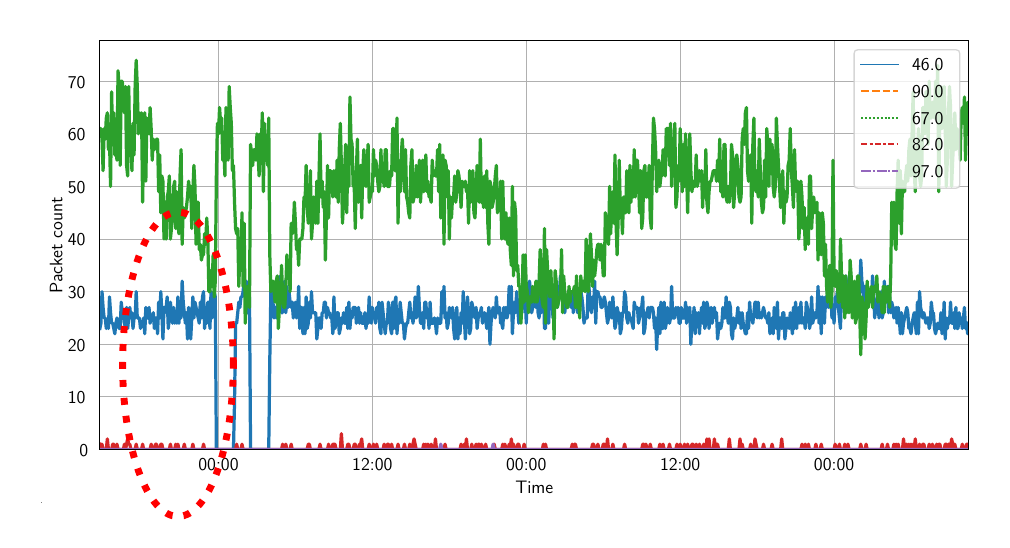
\begin{tikzpicture}
    \node(A){
    \resizebox{0.98\textwidth}{!}
        {
            %% Creator: Matplotlib, PGF backend
%%
%% To include the figure in your LaTeX document, write
%%   \input{<filename>.pgf}
%%
%% Make sure the required packages are loaded in your preamble
%%   \usepackage{pgf}
%%
%% Also ensure that all the required font packages are loaded; for instance,
%% the lmodern package is sometimes necessary when using math font.
%%   \usepackage{lmodern}
%%
%% Figures using additional raster images can only be included by \input if
%% they are in the same directory as the main LaTeX file. For loading figures
%% from other directories you can use the `import` package
%%   \usepackage{import}
%%
%% and then include the figures with
%%   \import{<path to file>}{<filename>.pgf}
%%
%% Matplotlib used the following preamble
%%   \usepackage{fontspec}
%%   \setmainfont{DejaVuSerif.ttf}[Path=\detokenize{/home/ankimme/fit/ibt/env/lib/python3.10/site-packages/matplotlib/mpl-data/fonts/ttf/}]
%%   \setsansfont{DejaVuSans.ttf}[Path=\detokenize{/home/ankimme/fit/ibt/env/lib/python3.10/site-packages/matplotlib/mpl-data/fonts/ttf/}]
%%   \setmonofont{DejaVuSansMono.ttf}[Path=\detokenize{/home/ankimme/fit/ibt/env/lib/python3.10/site-packages/matplotlib/mpl-data/fonts/ttf/}]
%%
\begingroup%
\makeatletter%
\begin{pgfpicture}%
\pgfpathrectangle{\pgfpointorigin}{\pgfqpoint{10.000000in}{5.000000in}}%
\pgfusepath{use as bounding box, clip}%
\begin{pgfscope}%
\pgfsetbuttcap%
\pgfsetmiterjoin%
\pgfsetlinewidth{0.000000pt}%
\definecolor{currentstroke}{rgb}{1.000000,1.000000,1.000000}%
\pgfsetstrokecolor{currentstroke}%
\pgfsetstrokeopacity{0.000000}%
\pgfsetdash{}{0pt}%
\pgfpathmoveto{\pgfqpoint{0.000000in}{0.000000in}}%
\pgfpathlineto{\pgfqpoint{10.000000in}{0.000000in}}%
\pgfpathlineto{\pgfqpoint{10.000000in}{5.000000in}}%
\pgfpathlineto{\pgfqpoint{0.000000in}{5.000000in}}%
\pgfpathlineto{\pgfqpoint{0.000000in}{0.000000in}}%
\pgfpathclose%
\pgfusepath{}%
\end{pgfscope}%
\begin{pgfscope}%
\pgfsetbuttcap%
\pgfsetmiterjoin%
\definecolor{currentfill}{rgb}{1.000000,1.000000,1.000000}%
\pgfsetfillcolor{currentfill}%
\pgfsetlinewidth{0.000000pt}%
\definecolor{currentstroke}{rgb}{0.000000,0.000000,0.000000}%
\pgfsetstrokecolor{currentstroke}%
\pgfsetstrokeopacity{0.000000}%
\pgfsetdash{}{0pt}%
\pgfpathmoveto{\pgfqpoint{0.630049in}{0.570804in}}%
\pgfpathlineto{\pgfqpoint{9.958330in}{0.570804in}}%
\pgfpathlineto{\pgfqpoint{9.958330in}{4.958330in}}%
\pgfpathlineto{\pgfqpoint{0.630049in}{4.958330in}}%
\pgfpathlineto{\pgfqpoint{0.630049in}{0.570804in}}%
\pgfpathclose%
\pgfusepath{fill}%
\end{pgfscope}%
\begin{pgfscope}%
\pgfpathrectangle{\pgfqpoint{0.630049in}{0.570804in}}{\pgfqpoint{9.328281in}{4.387526in}}%
\pgfusepath{clip}%
\pgfsetrectcap%
\pgfsetroundjoin%
\pgfsetlinewidth{0.803000pt}%
\definecolor{currentstroke}{rgb}{0.690196,0.690196,0.690196}%
\pgfsetstrokecolor{currentstroke}%
\pgfsetdash{}{0pt}%
\pgfpathmoveto{\pgfqpoint{1.903652in}{0.570804in}}%
\pgfpathlineto{\pgfqpoint{1.903652in}{4.958330in}}%
\pgfusepath{stroke}%
\end{pgfscope}%
\begin{pgfscope}%
\pgfsetbuttcap%
\pgfsetroundjoin%
\definecolor{currentfill}{rgb}{0.000000,0.000000,0.000000}%
\pgfsetfillcolor{currentfill}%
\pgfsetlinewidth{0.803000pt}%
\definecolor{currentstroke}{rgb}{0.000000,0.000000,0.000000}%
\pgfsetstrokecolor{currentstroke}%
\pgfsetdash{}{0pt}%
\pgfsys@defobject{currentmarker}{\pgfqpoint{0.000000in}{-0.048611in}}{\pgfqpoint{0.000000in}{0.000000in}}{%
\pgfpathmoveto{\pgfqpoint{0.000000in}{0.000000in}}%
\pgfpathlineto{\pgfqpoint{0.000000in}{-0.048611in}}%
\pgfusepath{stroke,fill}%
}%
\begin{pgfscope}%
\pgfsys@transformshift{1.903652in}{0.570804in}%
\pgfsys@useobject{currentmarker}{}%
\end{pgfscope}%
\end{pgfscope}%
\begin{pgfscope}%
\definecolor{textcolor}{rgb}{0.000000,0.000000,0.000000}%
\pgfsetstrokecolor{textcolor}%
\pgfsetfillcolor{textcolor}%
\pgftext[x=1.903652in,y=0.473582in,,top]{\color{textcolor}\sffamily\fontsize{14.000000}{16.800000}\selectfont 00:00}%
\end{pgfscope}%
\begin{pgfscope}%
\pgfpathrectangle{\pgfqpoint{0.630049in}{0.570804in}}{\pgfqpoint{9.328281in}{4.387526in}}%
\pgfusepath{clip}%
\pgfsetrectcap%
\pgfsetroundjoin%
\pgfsetlinewidth{0.803000pt}%
\definecolor{currentstroke}{rgb}{0.690196,0.690196,0.690196}%
\pgfsetstrokecolor{currentstroke}%
\pgfsetdash{}{0pt}%
\pgfpathmoveto{\pgfqpoint{3.555893in}{0.570804in}}%
\pgfpathlineto{\pgfqpoint{3.555893in}{4.958330in}}%
\pgfusepath{stroke}%
\end{pgfscope}%
\begin{pgfscope}%
\pgfsetbuttcap%
\pgfsetroundjoin%
\definecolor{currentfill}{rgb}{0.000000,0.000000,0.000000}%
\pgfsetfillcolor{currentfill}%
\pgfsetlinewidth{0.803000pt}%
\definecolor{currentstroke}{rgb}{0.000000,0.000000,0.000000}%
\pgfsetstrokecolor{currentstroke}%
\pgfsetdash{}{0pt}%
\pgfsys@defobject{currentmarker}{\pgfqpoint{0.000000in}{-0.048611in}}{\pgfqpoint{0.000000in}{0.000000in}}{%
\pgfpathmoveto{\pgfqpoint{0.000000in}{0.000000in}}%
\pgfpathlineto{\pgfqpoint{0.000000in}{-0.048611in}}%
\pgfusepath{stroke,fill}%
}%
\begin{pgfscope}%
\pgfsys@transformshift{3.555893in}{0.570804in}%
\pgfsys@useobject{currentmarker}{}%
\end{pgfscope}%
\end{pgfscope}%
\begin{pgfscope}%
\definecolor{textcolor}{rgb}{0.000000,0.000000,0.000000}%
\pgfsetstrokecolor{textcolor}%
\pgfsetfillcolor{textcolor}%
\pgftext[x=3.555893in,y=0.473582in,,top]{\color{textcolor}\sffamily\fontsize{14.000000}{16.800000}\selectfont 12:00}%
\end{pgfscope}%
\begin{pgfscope}%
\pgfpathrectangle{\pgfqpoint{0.630049in}{0.570804in}}{\pgfqpoint{9.328281in}{4.387526in}}%
\pgfusepath{clip}%
\pgfsetrectcap%
\pgfsetroundjoin%
\pgfsetlinewidth{0.803000pt}%
\definecolor{currentstroke}{rgb}{0.690196,0.690196,0.690196}%
\pgfsetstrokecolor{currentstroke}%
\pgfsetdash{}{0pt}%
\pgfpathmoveto{\pgfqpoint{5.208135in}{0.570804in}}%
\pgfpathlineto{\pgfqpoint{5.208135in}{4.958330in}}%
\pgfusepath{stroke}%
\end{pgfscope}%
\begin{pgfscope}%
\pgfsetbuttcap%
\pgfsetroundjoin%
\definecolor{currentfill}{rgb}{0.000000,0.000000,0.000000}%
\pgfsetfillcolor{currentfill}%
\pgfsetlinewidth{0.803000pt}%
\definecolor{currentstroke}{rgb}{0.000000,0.000000,0.000000}%
\pgfsetstrokecolor{currentstroke}%
\pgfsetdash{}{0pt}%
\pgfsys@defobject{currentmarker}{\pgfqpoint{0.000000in}{-0.048611in}}{\pgfqpoint{0.000000in}{0.000000in}}{%
\pgfpathmoveto{\pgfqpoint{0.000000in}{0.000000in}}%
\pgfpathlineto{\pgfqpoint{0.000000in}{-0.048611in}}%
\pgfusepath{stroke,fill}%
}%
\begin{pgfscope}%
\pgfsys@transformshift{5.208135in}{0.570804in}%
\pgfsys@useobject{currentmarker}{}%
\end{pgfscope}%
\end{pgfscope}%
\begin{pgfscope}%
\definecolor{textcolor}{rgb}{0.000000,0.000000,0.000000}%
\pgfsetstrokecolor{textcolor}%
\pgfsetfillcolor{textcolor}%
\pgftext[x=5.208135in,y=0.473582in,,top]{\color{textcolor}\sffamily\fontsize{14.000000}{16.800000}\selectfont 00:00}%
\end{pgfscope}%
\begin{pgfscope}%
\pgfpathrectangle{\pgfqpoint{0.630049in}{0.570804in}}{\pgfqpoint{9.328281in}{4.387526in}}%
\pgfusepath{clip}%
\pgfsetrectcap%
\pgfsetroundjoin%
\pgfsetlinewidth{0.803000pt}%
\definecolor{currentstroke}{rgb}{0.690196,0.690196,0.690196}%
\pgfsetstrokecolor{currentstroke}%
\pgfsetdash{}{0pt}%
\pgfpathmoveto{\pgfqpoint{6.860377in}{0.570804in}}%
\pgfpathlineto{\pgfqpoint{6.860377in}{4.958330in}}%
\pgfusepath{stroke}%
\end{pgfscope}%
\begin{pgfscope}%
\pgfsetbuttcap%
\pgfsetroundjoin%
\definecolor{currentfill}{rgb}{0.000000,0.000000,0.000000}%
\pgfsetfillcolor{currentfill}%
\pgfsetlinewidth{0.803000pt}%
\definecolor{currentstroke}{rgb}{0.000000,0.000000,0.000000}%
\pgfsetstrokecolor{currentstroke}%
\pgfsetdash{}{0pt}%
\pgfsys@defobject{currentmarker}{\pgfqpoint{0.000000in}{-0.048611in}}{\pgfqpoint{0.000000in}{0.000000in}}{%
\pgfpathmoveto{\pgfqpoint{0.000000in}{0.000000in}}%
\pgfpathlineto{\pgfqpoint{0.000000in}{-0.048611in}}%
\pgfusepath{stroke,fill}%
}%
\begin{pgfscope}%
\pgfsys@transformshift{6.860377in}{0.570804in}%
\pgfsys@useobject{currentmarker}{}%
\end{pgfscope}%
\end{pgfscope}%
\begin{pgfscope}%
\definecolor{textcolor}{rgb}{0.000000,0.000000,0.000000}%
\pgfsetstrokecolor{textcolor}%
\pgfsetfillcolor{textcolor}%
\pgftext[x=6.860377in,y=0.473582in,,top]{\color{textcolor}\sffamily\fontsize{14.000000}{16.800000}\selectfont 12:00}%
\end{pgfscope}%
\begin{pgfscope}%
\pgfpathrectangle{\pgfqpoint{0.630049in}{0.570804in}}{\pgfqpoint{9.328281in}{4.387526in}}%
\pgfusepath{clip}%
\pgfsetrectcap%
\pgfsetroundjoin%
\pgfsetlinewidth{0.803000pt}%
\definecolor{currentstroke}{rgb}{0.690196,0.690196,0.690196}%
\pgfsetstrokecolor{currentstroke}%
\pgfsetdash{}{0pt}%
\pgfpathmoveto{\pgfqpoint{8.512619in}{0.570804in}}%
\pgfpathlineto{\pgfqpoint{8.512619in}{4.958330in}}%
\pgfusepath{stroke}%
\end{pgfscope}%
\begin{pgfscope}%
\pgfsetbuttcap%
\pgfsetroundjoin%
\definecolor{currentfill}{rgb}{0.000000,0.000000,0.000000}%
\pgfsetfillcolor{currentfill}%
\pgfsetlinewidth{0.803000pt}%
\definecolor{currentstroke}{rgb}{0.000000,0.000000,0.000000}%
\pgfsetstrokecolor{currentstroke}%
\pgfsetdash{}{0pt}%
\pgfsys@defobject{currentmarker}{\pgfqpoint{0.000000in}{-0.048611in}}{\pgfqpoint{0.000000in}{0.000000in}}{%
\pgfpathmoveto{\pgfqpoint{0.000000in}{0.000000in}}%
\pgfpathlineto{\pgfqpoint{0.000000in}{-0.048611in}}%
\pgfusepath{stroke,fill}%
}%
\begin{pgfscope}%
\pgfsys@transformshift{8.512619in}{0.570804in}%
\pgfsys@useobject{currentmarker}{}%
\end{pgfscope}%
\end{pgfscope}%
\begin{pgfscope}%
\definecolor{textcolor}{rgb}{0.000000,0.000000,0.000000}%
\pgfsetstrokecolor{textcolor}%
\pgfsetfillcolor{textcolor}%
\pgftext[x=8.512619in,y=0.473582in,,top]{\color{textcolor}\sffamily\fontsize{14.000000}{16.800000}\selectfont 00:00}%
\end{pgfscope}%
\begin{pgfscope}%
\definecolor{textcolor}{rgb}{0.000000,0.000000,0.000000}%
\pgfsetstrokecolor{textcolor}%
\pgfsetfillcolor{textcolor}%
\pgftext[x=5.294189in,y=0.229848in,,top]{\color{textcolor}\sffamily\fontsize{14.000000}{16.800000}\selectfont Time}%
\end{pgfscope}%
\begin{pgfscope}%
\pgfpathrectangle{\pgfqpoint{0.630049in}{0.570804in}}{\pgfqpoint{9.328281in}{4.387526in}}%
\pgfusepath{clip}%
\pgfsetrectcap%
\pgfsetroundjoin%
\pgfsetlinewidth{0.803000pt}%
\definecolor{currentstroke}{rgb}{0.690196,0.690196,0.690196}%
\pgfsetstrokecolor{currentstroke}%
\pgfsetdash{}{0pt}%
\pgfpathmoveto{\pgfqpoint{0.630049in}{0.570804in}}%
\pgfpathlineto{\pgfqpoint{9.958330in}{0.570804in}}%
\pgfusepath{stroke}%
\end{pgfscope}%
\begin{pgfscope}%
\pgfsetbuttcap%
\pgfsetroundjoin%
\definecolor{currentfill}{rgb}{0.000000,0.000000,0.000000}%
\pgfsetfillcolor{currentfill}%
\pgfsetlinewidth{0.803000pt}%
\definecolor{currentstroke}{rgb}{0.000000,0.000000,0.000000}%
\pgfsetstrokecolor{currentstroke}%
\pgfsetdash{}{0pt}%
\pgfsys@defobject{currentmarker}{\pgfqpoint{-0.048611in}{0.000000in}}{\pgfqpoint{-0.000000in}{0.000000in}}{%
\pgfpathmoveto{\pgfqpoint{-0.000000in}{0.000000in}}%
\pgfpathlineto{\pgfqpoint{-0.048611in}{0.000000in}}%
\pgfusepath{stroke,fill}%
}%
\begin{pgfscope}%
\pgfsys@transformshift{0.630049in}{0.570804in}%
\pgfsys@useobject{currentmarker}{}%
\end{pgfscope}%
\end{pgfscope}%
\begin{pgfscope}%
\definecolor{textcolor}{rgb}{0.000000,0.000000,0.000000}%
\pgfsetstrokecolor{textcolor}%
\pgfsetfillcolor{textcolor}%
\pgftext[x=0.409115in, y=0.496938in, left, base]{\color{textcolor}\sffamily\fontsize{14.000000}{16.800000}\selectfont 0}%
\end{pgfscope}%
\begin{pgfscope}%
\pgfpathrectangle{\pgfqpoint{0.630049in}{0.570804in}}{\pgfqpoint{9.328281in}{4.387526in}}%
\pgfusepath{clip}%
\pgfsetrectcap%
\pgfsetroundjoin%
\pgfsetlinewidth{0.803000pt}%
\definecolor{currentstroke}{rgb}{0.690196,0.690196,0.690196}%
\pgfsetstrokecolor{currentstroke}%
\pgfsetdash{}{0pt}%
\pgfpathmoveto{\pgfqpoint{0.630049in}{1.135479in}}%
\pgfpathlineto{\pgfqpoint{9.958330in}{1.135479in}}%
\pgfusepath{stroke}%
\end{pgfscope}%
\begin{pgfscope}%
\pgfsetbuttcap%
\pgfsetroundjoin%
\definecolor{currentfill}{rgb}{0.000000,0.000000,0.000000}%
\pgfsetfillcolor{currentfill}%
\pgfsetlinewidth{0.803000pt}%
\definecolor{currentstroke}{rgb}{0.000000,0.000000,0.000000}%
\pgfsetstrokecolor{currentstroke}%
\pgfsetdash{}{0pt}%
\pgfsys@defobject{currentmarker}{\pgfqpoint{-0.048611in}{0.000000in}}{\pgfqpoint{-0.000000in}{0.000000in}}{%
\pgfpathmoveto{\pgfqpoint{-0.000000in}{0.000000in}}%
\pgfpathlineto{\pgfqpoint{-0.048611in}{0.000000in}}%
\pgfusepath{stroke,fill}%
}%
\begin{pgfscope}%
\pgfsys@transformshift{0.630049in}{1.135479in}%
\pgfsys@useobject{currentmarker}{}%
\end{pgfscope}%
\end{pgfscope}%
\begin{pgfscope}%
\definecolor{textcolor}{rgb}{0.000000,0.000000,0.000000}%
\pgfsetstrokecolor{textcolor}%
\pgfsetfillcolor{textcolor}%
\pgftext[x=0.285404in, y=1.061613in, left, base]{\color{textcolor}\sffamily\fontsize{14.000000}{16.800000}\selectfont 10}%
\end{pgfscope}%
\begin{pgfscope}%
\pgfpathrectangle{\pgfqpoint{0.630049in}{0.570804in}}{\pgfqpoint{9.328281in}{4.387526in}}%
\pgfusepath{clip}%
\pgfsetrectcap%
\pgfsetroundjoin%
\pgfsetlinewidth{0.803000pt}%
\definecolor{currentstroke}{rgb}{0.690196,0.690196,0.690196}%
\pgfsetstrokecolor{currentstroke}%
\pgfsetdash{}{0pt}%
\pgfpathmoveto{\pgfqpoint{0.630049in}{1.700154in}}%
\pgfpathlineto{\pgfqpoint{9.958330in}{1.700154in}}%
\pgfusepath{stroke}%
\end{pgfscope}%
\begin{pgfscope}%
\pgfsetbuttcap%
\pgfsetroundjoin%
\definecolor{currentfill}{rgb}{0.000000,0.000000,0.000000}%
\pgfsetfillcolor{currentfill}%
\pgfsetlinewidth{0.803000pt}%
\definecolor{currentstroke}{rgb}{0.000000,0.000000,0.000000}%
\pgfsetstrokecolor{currentstroke}%
\pgfsetdash{}{0pt}%
\pgfsys@defobject{currentmarker}{\pgfqpoint{-0.048611in}{0.000000in}}{\pgfqpoint{-0.000000in}{0.000000in}}{%
\pgfpathmoveto{\pgfqpoint{-0.000000in}{0.000000in}}%
\pgfpathlineto{\pgfqpoint{-0.048611in}{0.000000in}}%
\pgfusepath{stroke,fill}%
}%
\begin{pgfscope}%
\pgfsys@transformshift{0.630049in}{1.700154in}%
\pgfsys@useobject{currentmarker}{}%
\end{pgfscope}%
\end{pgfscope}%
\begin{pgfscope}%
\definecolor{textcolor}{rgb}{0.000000,0.000000,0.000000}%
\pgfsetstrokecolor{textcolor}%
\pgfsetfillcolor{textcolor}%
\pgftext[x=0.285404in, y=1.626288in, left, base]{\color{textcolor}\sffamily\fontsize{14.000000}{16.800000}\selectfont 20}%
\end{pgfscope}%
\begin{pgfscope}%
\pgfpathrectangle{\pgfqpoint{0.630049in}{0.570804in}}{\pgfqpoint{9.328281in}{4.387526in}}%
\pgfusepath{clip}%
\pgfsetrectcap%
\pgfsetroundjoin%
\pgfsetlinewidth{0.803000pt}%
\definecolor{currentstroke}{rgb}{0.690196,0.690196,0.690196}%
\pgfsetstrokecolor{currentstroke}%
\pgfsetdash{}{0pt}%
\pgfpathmoveto{\pgfqpoint{0.630049in}{2.264829in}}%
\pgfpathlineto{\pgfqpoint{9.958330in}{2.264829in}}%
\pgfusepath{stroke}%
\end{pgfscope}%
\begin{pgfscope}%
\pgfsetbuttcap%
\pgfsetroundjoin%
\definecolor{currentfill}{rgb}{0.000000,0.000000,0.000000}%
\pgfsetfillcolor{currentfill}%
\pgfsetlinewidth{0.803000pt}%
\definecolor{currentstroke}{rgb}{0.000000,0.000000,0.000000}%
\pgfsetstrokecolor{currentstroke}%
\pgfsetdash{}{0pt}%
\pgfsys@defobject{currentmarker}{\pgfqpoint{-0.048611in}{0.000000in}}{\pgfqpoint{-0.000000in}{0.000000in}}{%
\pgfpathmoveto{\pgfqpoint{-0.000000in}{0.000000in}}%
\pgfpathlineto{\pgfqpoint{-0.048611in}{0.000000in}}%
\pgfusepath{stroke,fill}%
}%
\begin{pgfscope}%
\pgfsys@transformshift{0.630049in}{2.264829in}%
\pgfsys@useobject{currentmarker}{}%
\end{pgfscope}%
\end{pgfscope}%
\begin{pgfscope}%
\definecolor{textcolor}{rgb}{0.000000,0.000000,0.000000}%
\pgfsetstrokecolor{textcolor}%
\pgfsetfillcolor{textcolor}%
\pgftext[x=0.285404in, y=2.190963in, left, base]{\color{textcolor}\sffamily\fontsize{14.000000}{16.800000}\selectfont 30}%
\end{pgfscope}%
\begin{pgfscope}%
\pgfpathrectangle{\pgfqpoint{0.630049in}{0.570804in}}{\pgfqpoint{9.328281in}{4.387526in}}%
\pgfusepath{clip}%
\pgfsetrectcap%
\pgfsetroundjoin%
\pgfsetlinewidth{0.803000pt}%
\definecolor{currentstroke}{rgb}{0.690196,0.690196,0.690196}%
\pgfsetstrokecolor{currentstroke}%
\pgfsetdash{}{0pt}%
\pgfpathmoveto{\pgfqpoint{0.630049in}{2.829505in}}%
\pgfpathlineto{\pgfqpoint{9.958330in}{2.829505in}}%
\pgfusepath{stroke}%
\end{pgfscope}%
\begin{pgfscope}%
\pgfsetbuttcap%
\pgfsetroundjoin%
\definecolor{currentfill}{rgb}{0.000000,0.000000,0.000000}%
\pgfsetfillcolor{currentfill}%
\pgfsetlinewidth{0.803000pt}%
\definecolor{currentstroke}{rgb}{0.000000,0.000000,0.000000}%
\pgfsetstrokecolor{currentstroke}%
\pgfsetdash{}{0pt}%
\pgfsys@defobject{currentmarker}{\pgfqpoint{-0.048611in}{0.000000in}}{\pgfqpoint{-0.000000in}{0.000000in}}{%
\pgfpathmoveto{\pgfqpoint{-0.000000in}{0.000000in}}%
\pgfpathlineto{\pgfqpoint{-0.048611in}{0.000000in}}%
\pgfusepath{stroke,fill}%
}%
\begin{pgfscope}%
\pgfsys@transformshift{0.630049in}{2.829505in}%
\pgfsys@useobject{currentmarker}{}%
\end{pgfscope}%
\end{pgfscope}%
\begin{pgfscope}%
\definecolor{textcolor}{rgb}{0.000000,0.000000,0.000000}%
\pgfsetstrokecolor{textcolor}%
\pgfsetfillcolor{textcolor}%
\pgftext[x=0.285404in, y=2.755638in, left, base]{\color{textcolor}\sffamily\fontsize{14.000000}{16.800000}\selectfont 40}%
\end{pgfscope}%
\begin{pgfscope}%
\pgfpathrectangle{\pgfqpoint{0.630049in}{0.570804in}}{\pgfqpoint{9.328281in}{4.387526in}}%
\pgfusepath{clip}%
\pgfsetrectcap%
\pgfsetroundjoin%
\pgfsetlinewidth{0.803000pt}%
\definecolor{currentstroke}{rgb}{0.690196,0.690196,0.690196}%
\pgfsetstrokecolor{currentstroke}%
\pgfsetdash{}{0pt}%
\pgfpathmoveto{\pgfqpoint{0.630049in}{3.394180in}}%
\pgfpathlineto{\pgfqpoint{9.958330in}{3.394180in}}%
\pgfusepath{stroke}%
\end{pgfscope}%
\begin{pgfscope}%
\pgfsetbuttcap%
\pgfsetroundjoin%
\definecolor{currentfill}{rgb}{0.000000,0.000000,0.000000}%
\pgfsetfillcolor{currentfill}%
\pgfsetlinewidth{0.803000pt}%
\definecolor{currentstroke}{rgb}{0.000000,0.000000,0.000000}%
\pgfsetstrokecolor{currentstroke}%
\pgfsetdash{}{0pt}%
\pgfsys@defobject{currentmarker}{\pgfqpoint{-0.048611in}{0.000000in}}{\pgfqpoint{-0.000000in}{0.000000in}}{%
\pgfpathmoveto{\pgfqpoint{-0.000000in}{0.000000in}}%
\pgfpathlineto{\pgfqpoint{-0.048611in}{0.000000in}}%
\pgfusepath{stroke,fill}%
}%
\begin{pgfscope}%
\pgfsys@transformshift{0.630049in}{3.394180in}%
\pgfsys@useobject{currentmarker}{}%
\end{pgfscope}%
\end{pgfscope}%
\begin{pgfscope}%
\definecolor{textcolor}{rgb}{0.000000,0.000000,0.000000}%
\pgfsetstrokecolor{textcolor}%
\pgfsetfillcolor{textcolor}%
\pgftext[x=0.285404in, y=3.320314in, left, base]{\color{textcolor}\sffamily\fontsize{14.000000}{16.800000}\selectfont 50}%
\end{pgfscope}%
\begin{pgfscope}%
\pgfpathrectangle{\pgfqpoint{0.630049in}{0.570804in}}{\pgfqpoint{9.328281in}{4.387526in}}%
\pgfusepath{clip}%
\pgfsetrectcap%
\pgfsetroundjoin%
\pgfsetlinewidth{0.803000pt}%
\definecolor{currentstroke}{rgb}{0.690196,0.690196,0.690196}%
\pgfsetstrokecolor{currentstroke}%
\pgfsetdash{}{0pt}%
\pgfpathmoveto{\pgfqpoint{0.630049in}{3.958855in}}%
\pgfpathlineto{\pgfqpoint{9.958330in}{3.958855in}}%
\pgfusepath{stroke}%
\end{pgfscope}%
\begin{pgfscope}%
\pgfsetbuttcap%
\pgfsetroundjoin%
\definecolor{currentfill}{rgb}{0.000000,0.000000,0.000000}%
\pgfsetfillcolor{currentfill}%
\pgfsetlinewidth{0.803000pt}%
\definecolor{currentstroke}{rgb}{0.000000,0.000000,0.000000}%
\pgfsetstrokecolor{currentstroke}%
\pgfsetdash{}{0pt}%
\pgfsys@defobject{currentmarker}{\pgfqpoint{-0.048611in}{0.000000in}}{\pgfqpoint{-0.000000in}{0.000000in}}{%
\pgfpathmoveto{\pgfqpoint{-0.000000in}{0.000000in}}%
\pgfpathlineto{\pgfqpoint{-0.048611in}{0.000000in}}%
\pgfusepath{stroke,fill}%
}%
\begin{pgfscope}%
\pgfsys@transformshift{0.630049in}{3.958855in}%
\pgfsys@useobject{currentmarker}{}%
\end{pgfscope}%
\end{pgfscope}%
\begin{pgfscope}%
\definecolor{textcolor}{rgb}{0.000000,0.000000,0.000000}%
\pgfsetstrokecolor{textcolor}%
\pgfsetfillcolor{textcolor}%
\pgftext[x=0.285404in, y=3.884989in, left, base]{\color{textcolor}\sffamily\fontsize{14.000000}{16.800000}\selectfont 60}%
\end{pgfscope}%
\begin{pgfscope}%
\pgfpathrectangle{\pgfqpoint{0.630049in}{0.570804in}}{\pgfqpoint{9.328281in}{4.387526in}}%
\pgfusepath{clip}%
\pgfsetrectcap%
\pgfsetroundjoin%
\pgfsetlinewidth{0.803000pt}%
\definecolor{currentstroke}{rgb}{0.690196,0.690196,0.690196}%
\pgfsetstrokecolor{currentstroke}%
\pgfsetdash{}{0pt}%
\pgfpathmoveto{\pgfqpoint{0.630049in}{4.523530in}}%
\pgfpathlineto{\pgfqpoint{9.958330in}{4.523530in}}%
\pgfusepath{stroke}%
\end{pgfscope}%
\begin{pgfscope}%
\pgfsetbuttcap%
\pgfsetroundjoin%
\definecolor{currentfill}{rgb}{0.000000,0.000000,0.000000}%
\pgfsetfillcolor{currentfill}%
\pgfsetlinewidth{0.803000pt}%
\definecolor{currentstroke}{rgb}{0.000000,0.000000,0.000000}%
\pgfsetstrokecolor{currentstroke}%
\pgfsetdash{}{0pt}%
\pgfsys@defobject{currentmarker}{\pgfqpoint{-0.048611in}{0.000000in}}{\pgfqpoint{-0.000000in}{0.000000in}}{%
\pgfpathmoveto{\pgfqpoint{-0.000000in}{0.000000in}}%
\pgfpathlineto{\pgfqpoint{-0.048611in}{0.000000in}}%
\pgfusepath{stroke,fill}%
}%
\begin{pgfscope}%
\pgfsys@transformshift{0.630049in}{4.523530in}%
\pgfsys@useobject{currentmarker}{}%
\end{pgfscope}%
\end{pgfscope}%
\begin{pgfscope}%
\definecolor{textcolor}{rgb}{0.000000,0.000000,0.000000}%
\pgfsetstrokecolor{textcolor}%
\pgfsetfillcolor{textcolor}%
\pgftext[x=0.285404in, y=4.449664in, left, base]{\color{textcolor}\sffamily\fontsize{14.000000}{16.800000}\selectfont 70}%
\end{pgfscope}%
\begin{pgfscope}%
\definecolor{textcolor}{rgb}{0.000000,0.000000,0.000000}%
\pgfsetstrokecolor{textcolor}%
\pgfsetfillcolor{textcolor}%
\pgftext[x=0.229848in,y=2.764567in,,bottom,rotate=90.000000]{\color{textcolor}\sffamily\fontsize{14.000000}{16.800000}\selectfont Packet count}%
\end{pgfscope}%
\begin{pgfscope}%
\pgfpathrectangle{\pgfqpoint{0.630049in}{0.570804in}}{\pgfqpoint{9.328281in}{4.387526in}}%
\pgfusepath{clip}%
\pgfsetrectcap%
\pgfsetroundjoin%
\pgfsetlinewidth{2.509375pt}%
\definecolor{currentstroke}{rgb}{0.121569,0.466667,0.705882}%
\pgfsetstrokecolor{currentstroke}%
\pgfsetdash{}{0pt}%
\pgfpathmoveto{\pgfqpoint{0.630049in}{1.869557in}}%
\pgfpathlineto{\pgfqpoint{0.641523in}{1.926024in}}%
\pgfpathlineto{\pgfqpoint{0.652997in}{2.264829in}}%
\pgfpathlineto{\pgfqpoint{0.664470in}{2.095427in}}%
\pgfpathlineto{\pgfqpoint{0.675944in}{1.982492in}}%
\pgfpathlineto{\pgfqpoint{0.687418in}{1.982492in}}%
\pgfpathlineto{\pgfqpoint{0.698892in}{1.869557in}}%
\pgfpathlineto{\pgfqpoint{0.710366in}{1.926024in}}%
\pgfpathlineto{\pgfqpoint{0.721840in}{1.869557in}}%
\pgfpathlineto{\pgfqpoint{0.733314in}{2.208362in}}%
\pgfpathlineto{\pgfqpoint{0.744788in}{2.038959in}}%
\pgfpathlineto{\pgfqpoint{0.756262in}{1.926024in}}%
\pgfpathlineto{\pgfqpoint{0.767736in}{1.926024in}}%
\pgfpathlineto{\pgfqpoint{0.790683in}{1.813089in}}%
\pgfpathlineto{\pgfqpoint{0.802157in}{1.926024in}}%
\pgfpathlineto{\pgfqpoint{0.813631in}{1.982492in}}%
\pgfpathlineto{\pgfqpoint{0.836579in}{1.869557in}}%
\pgfpathlineto{\pgfqpoint{0.848053in}{1.869557in}}%
\pgfpathlineto{\pgfqpoint{0.859527in}{2.151894in}}%
\pgfpathlineto{\pgfqpoint{0.871001in}{2.038959in}}%
\pgfpathlineto{\pgfqpoint{0.882475in}{2.038959in}}%
\pgfpathlineto{\pgfqpoint{0.893948in}{1.926024in}}%
\pgfpathlineto{\pgfqpoint{0.905422in}{1.869557in}}%
\pgfpathlineto{\pgfqpoint{0.916896in}{2.095427in}}%
\pgfpathlineto{\pgfqpoint{0.928370in}{1.869557in}}%
\pgfpathlineto{\pgfqpoint{0.951318in}{2.095427in}}%
\pgfpathlineto{\pgfqpoint{0.962792in}{1.982492in}}%
\pgfpathlineto{\pgfqpoint{0.974266in}{2.038959in}}%
\pgfpathlineto{\pgfqpoint{0.985740in}{1.869557in}}%
\pgfpathlineto{\pgfqpoint{0.997214in}{1.982492in}}%
\pgfpathlineto{\pgfqpoint{1.008687in}{1.982492in}}%
\pgfpathlineto{\pgfqpoint{1.020161in}{2.264829in}}%
\pgfpathlineto{\pgfqpoint{1.031635in}{1.982492in}}%
\pgfpathlineto{\pgfqpoint{1.054583in}{1.982492in}}%
\pgfpathlineto{\pgfqpoint{1.066057in}{1.869557in}}%
\pgfpathlineto{\pgfqpoint{1.077531in}{1.926024in}}%
\pgfpathlineto{\pgfqpoint{1.089005in}{1.926024in}}%
\pgfpathlineto{\pgfqpoint{1.100479in}{1.982492in}}%
\pgfpathlineto{\pgfqpoint{1.111953in}{1.813089in}}%
\pgfpathlineto{\pgfqpoint{1.123426in}{2.095427in}}%
\pgfpathlineto{\pgfqpoint{1.134900in}{1.982492in}}%
\pgfpathlineto{\pgfqpoint{1.146374in}{1.982492in}}%
\pgfpathlineto{\pgfqpoint{1.157848in}{2.095427in}}%
\pgfpathlineto{\pgfqpoint{1.169322in}{1.926024in}}%
\pgfpathlineto{\pgfqpoint{1.180796in}{1.982492in}}%
\pgfpathlineto{\pgfqpoint{1.192270in}{1.982492in}}%
\pgfpathlineto{\pgfqpoint{1.203744in}{2.038959in}}%
\pgfpathlineto{\pgfqpoint{1.215218in}{1.869557in}}%
\pgfpathlineto{\pgfqpoint{1.226692in}{1.982492in}}%
\pgfpathlineto{\pgfqpoint{1.238165in}{1.982492in}}%
\pgfpathlineto{\pgfqpoint{1.249639in}{1.813089in}}%
\pgfpathlineto{\pgfqpoint{1.261113in}{2.151894in}}%
\pgfpathlineto{\pgfqpoint{1.272587in}{1.982492in}}%
\pgfpathlineto{\pgfqpoint{1.284061in}{2.264829in}}%
\pgfpathlineto{\pgfqpoint{1.295535in}{2.038959in}}%
\pgfpathlineto{\pgfqpoint{1.307009in}{1.756622in}}%
\pgfpathlineto{\pgfqpoint{1.318483in}{2.095427in}}%
\pgfpathlineto{\pgfqpoint{1.329957in}{2.038959in}}%
\pgfpathlineto{\pgfqpoint{1.341431in}{2.095427in}}%
\pgfpathlineto{\pgfqpoint{1.352904in}{2.208362in}}%
\pgfpathlineto{\pgfqpoint{1.364378in}{1.869557in}}%
\pgfpathlineto{\pgfqpoint{1.375852in}{1.982492in}}%
\pgfpathlineto{\pgfqpoint{1.387326in}{2.151894in}}%
\pgfpathlineto{\pgfqpoint{1.410274in}{1.926024in}}%
\pgfpathlineto{\pgfqpoint{1.421748in}{2.095427in}}%
\pgfpathlineto{\pgfqpoint{1.433222in}{1.926024in}}%
\pgfpathlineto{\pgfqpoint{1.444696in}{1.982492in}}%
\pgfpathlineto{\pgfqpoint{1.456170in}{1.926024in}}%
\pgfpathlineto{\pgfqpoint{1.467643in}{2.208362in}}%
\pgfpathlineto{\pgfqpoint{1.479117in}{1.926024in}}%
\pgfpathlineto{\pgfqpoint{1.490591in}{2.151894in}}%
\pgfpathlineto{\pgfqpoint{1.502065in}{1.982492in}}%
\pgfpathlineto{\pgfqpoint{1.513539in}{2.377764in}}%
\pgfpathlineto{\pgfqpoint{1.525013in}{2.151894in}}%
\pgfpathlineto{\pgfqpoint{1.547961in}{1.926024in}}%
\pgfpathlineto{\pgfqpoint{1.559435in}{2.038959in}}%
\pgfpathlineto{\pgfqpoint{1.570909in}{1.756622in}}%
\pgfpathlineto{\pgfqpoint{1.582383in}{2.095427in}}%
\pgfpathlineto{\pgfqpoint{1.593856in}{2.038959in}}%
\pgfpathlineto{\pgfqpoint{1.605330in}{1.756622in}}%
\pgfpathlineto{\pgfqpoint{1.628278in}{2.208362in}}%
\pgfpathlineto{\pgfqpoint{1.639752in}{1.982492in}}%
\pgfpathlineto{\pgfqpoint{1.651226in}{2.151894in}}%
\pgfpathlineto{\pgfqpoint{1.697122in}{1.926024in}}%
\pgfpathlineto{\pgfqpoint{1.708595in}{2.151894in}}%
\pgfpathlineto{\pgfqpoint{1.720069in}{1.982492in}}%
\pgfpathlineto{\pgfqpoint{1.731543in}{2.208362in}}%
\pgfpathlineto{\pgfqpoint{1.743017in}{2.264829in}}%
\pgfpathlineto{\pgfqpoint{1.754491in}{1.869557in}}%
\pgfpathlineto{\pgfqpoint{1.765965in}{2.038959in}}%
\pgfpathlineto{\pgfqpoint{1.777439in}{1.926024in}}%
\pgfpathlineto{\pgfqpoint{1.788913in}{2.151894in}}%
\pgfpathlineto{\pgfqpoint{1.800387in}{2.151894in}}%
\pgfpathlineto{\pgfqpoint{1.811861in}{1.869557in}}%
\pgfpathlineto{\pgfqpoint{1.823334in}{2.264829in}}%
\pgfpathlineto{\pgfqpoint{1.834808in}{1.982492in}}%
\pgfpathlineto{\pgfqpoint{1.846282in}{2.095427in}}%
\pgfpathlineto{\pgfqpoint{1.857756in}{2.264829in}}%
\pgfpathlineto{\pgfqpoint{1.869230in}{2.208362in}}%
\pgfpathlineto{\pgfqpoint{1.880704in}{0.570804in}}%
\pgfpathlineto{\pgfqpoint{2.064286in}{0.570804in}}%
\pgfpathlineto{\pgfqpoint{2.075760in}{1.079012in}}%
\pgfpathlineto{\pgfqpoint{2.087234in}{1.926024in}}%
\pgfpathlineto{\pgfqpoint{2.098708in}{1.926024in}}%
\pgfpathlineto{\pgfqpoint{2.121656in}{2.151894in}}%
\pgfpathlineto{\pgfqpoint{2.133130in}{2.095427in}}%
\pgfpathlineto{\pgfqpoint{2.144604in}{2.208362in}}%
\pgfpathlineto{\pgfqpoint{2.156078in}{2.208362in}}%
\pgfpathlineto{\pgfqpoint{2.167551in}{2.264829in}}%
\pgfpathlineto{\pgfqpoint{2.179025in}{2.377764in}}%
\pgfpathlineto{\pgfqpoint{2.190499in}{2.208362in}}%
\pgfpathlineto{\pgfqpoint{2.201973in}{2.377764in}}%
\pgfpathlineto{\pgfqpoint{2.213447in}{2.038959in}}%
\pgfpathlineto{\pgfqpoint{2.224921in}{2.208362in}}%
\pgfpathlineto{\pgfqpoint{2.236395in}{2.208362in}}%
\pgfpathlineto{\pgfqpoint{2.247869in}{0.570804in}}%
\pgfpathlineto{\pgfqpoint{2.442925in}{0.570804in}}%
\pgfpathlineto{\pgfqpoint{2.454399in}{1.530752in}}%
\pgfpathlineto{\pgfqpoint{2.465873in}{2.264829in}}%
\pgfpathlineto{\pgfqpoint{2.477347in}{2.321297in}}%
\pgfpathlineto{\pgfqpoint{2.500295in}{1.982492in}}%
\pgfpathlineto{\pgfqpoint{2.511768in}{2.095427in}}%
\pgfpathlineto{\pgfqpoint{2.523242in}{1.982492in}}%
\pgfpathlineto{\pgfqpoint{2.534716in}{2.095427in}}%
\pgfpathlineto{\pgfqpoint{2.546190in}{2.321297in}}%
\pgfpathlineto{\pgfqpoint{2.557664in}{2.151894in}}%
\pgfpathlineto{\pgfqpoint{2.569138in}{2.434232in}}%
\pgfpathlineto{\pgfqpoint{2.580612in}{2.038959in}}%
\pgfpathlineto{\pgfqpoint{2.592086in}{2.038959in}}%
\pgfpathlineto{\pgfqpoint{2.603560in}{2.264829in}}%
\pgfpathlineto{\pgfqpoint{2.615034in}{2.377764in}}%
\pgfpathlineto{\pgfqpoint{2.626507in}{2.038959in}}%
\pgfpathlineto{\pgfqpoint{2.637981in}{2.321297in}}%
\pgfpathlineto{\pgfqpoint{2.649455in}{2.095427in}}%
\pgfpathlineto{\pgfqpoint{2.660929in}{2.264829in}}%
\pgfpathlineto{\pgfqpoint{2.672403in}{2.151894in}}%
\pgfpathlineto{\pgfqpoint{2.683877in}{2.095427in}}%
\pgfpathlineto{\pgfqpoint{2.695351in}{2.151894in}}%
\pgfpathlineto{\pgfqpoint{2.706825in}{1.982492in}}%
\pgfpathlineto{\pgfqpoint{2.718299in}{2.095427in}}%
\pgfpathlineto{\pgfqpoint{2.729773in}{2.151894in}}%
\pgfpathlineto{\pgfqpoint{2.741246in}{1.982492in}}%
\pgfpathlineto{\pgfqpoint{2.752720in}{2.038959in}}%
\pgfpathlineto{\pgfqpoint{2.764194in}{2.321297in}}%
\pgfpathlineto{\pgfqpoint{2.775668in}{1.869557in}}%
\pgfpathlineto{\pgfqpoint{2.787142in}{2.095427in}}%
\pgfpathlineto{\pgfqpoint{2.798616in}{2.095427in}}%
\pgfpathlineto{\pgfqpoint{2.810090in}{1.813089in}}%
\pgfpathlineto{\pgfqpoint{2.821564in}{2.095427in}}%
\pgfpathlineto{\pgfqpoint{2.833038in}{1.813089in}}%
\pgfpathlineto{\pgfqpoint{2.844512in}{2.208362in}}%
\pgfpathlineto{\pgfqpoint{2.855985in}{1.869557in}}%
\pgfpathlineto{\pgfqpoint{2.867459in}{1.926024in}}%
\pgfpathlineto{\pgfqpoint{2.878933in}{2.151894in}}%
\pgfpathlineto{\pgfqpoint{2.890407in}{1.982492in}}%
\pgfpathlineto{\pgfqpoint{2.901881in}{2.264829in}}%
\pgfpathlineto{\pgfqpoint{2.913355in}{2.038959in}}%
\pgfpathlineto{\pgfqpoint{2.947777in}{2.038959in}}%
\pgfpathlineto{\pgfqpoint{2.959251in}{1.756622in}}%
\pgfpathlineto{\pgfqpoint{2.982198in}{1.982492in}}%
\pgfpathlineto{\pgfqpoint{2.993672in}{1.982492in}}%
\pgfpathlineto{\pgfqpoint{3.005146in}{1.869557in}}%
\pgfpathlineto{\pgfqpoint{3.016620in}{2.038959in}}%
\pgfpathlineto{\pgfqpoint{3.028094in}{2.038959in}}%
\pgfpathlineto{\pgfqpoint{3.039568in}{2.151894in}}%
\pgfpathlineto{\pgfqpoint{3.051042in}{2.151894in}}%
\pgfpathlineto{\pgfqpoint{3.062516in}{1.982492in}}%
\pgfpathlineto{\pgfqpoint{3.073990in}{2.095427in}}%
\pgfpathlineto{\pgfqpoint{3.085463in}{2.038959in}}%
\pgfpathlineto{\pgfqpoint{3.096937in}{2.038959in}}%
\pgfpathlineto{\pgfqpoint{3.108411in}{1.982492in}}%
\pgfpathlineto{\pgfqpoint{3.119885in}{1.982492in}}%
\pgfpathlineto{\pgfqpoint{3.131359in}{1.813089in}}%
\pgfpathlineto{\pgfqpoint{3.142833in}{2.208362in}}%
\pgfpathlineto{\pgfqpoint{3.154307in}{1.869557in}}%
\pgfpathlineto{\pgfqpoint{3.165781in}{1.926024in}}%
\pgfpathlineto{\pgfqpoint{3.177255in}{2.038959in}}%
\pgfpathlineto{\pgfqpoint{3.188729in}{2.038959in}}%
\pgfpathlineto{\pgfqpoint{3.200203in}{1.813089in}}%
\pgfpathlineto{\pgfqpoint{3.211676in}{1.869557in}}%
\pgfpathlineto{\pgfqpoint{3.223150in}{1.982492in}}%
\pgfpathlineto{\pgfqpoint{3.234624in}{1.926024in}}%
\pgfpathlineto{\pgfqpoint{3.246098in}{2.038959in}}%
\pgfpathlineto{\pgfqpoint{3.257572in}{1.926024in}}%
\pgfpathlineto{\pgfqpoint{3.269046in}{1.926024in}}%
\pgfpathlineto{\pgfqpoint{3.280520in}{2.095427in}}%
\pgfpathlineto{\pgfqpoint{3.291994in}{1.869557in}}%
\pgfpathlineto{\pgfqpoint{3.303468in}{2.151894in}}%
\pgfpathlineto{\pgfqpoint{3.314942in}{1.869557in}}%
\pgfpathlineto{\pgfqpoint{3.326415in}{2.038959in}}%
\pgfpathlineto{\pgfqpoint{3.337889in}{1.982492in}}%
\pgfpathlineto{\pgfqpoint{3.349363in}{2.095427in}}%
\pgfpathlineto{\pgfqpoint{3.372311in}{2.095427in}}%
\pgfpathlineto{\pgfqpoint{3.383785in}{1.926024in}}%
\pgfpathlineto{\pgfqpoint{3.395259in}{1.982492in}}%
\pgfpathlineto{\pgfqpoint{3.406733in}{2.095427in}}%
\pgfpathlineto{\pgfqpoint{3.418207in}{1.926024in}}%
\pgfpathlineto{\pgfqpoint{3.429681in}{2.038959in}}%
\pgfpathlineto{\pgfqpoint{3.441154in}{1.926024in}}%
\pgfpathlineto{\pgfqpoint{3.464102in}{1.926024in}}%
\pgfpathlineto{\pgfqpoint{3.475576in}{2.038959in}}%
\pgfpathlineto{\pgfqpoint{3.487050in}{1.869557in}}%
\pgfpathlineto{\pgfqpoint{3.498524in}{1.982492in}}%
\pgfpathlineto{\pgfqpoint{3.509998in}{1.926024in}}%
\pgfpathlineto{\pgfqpoint{3.521472in}{2.208362in}}%
\pgfpathlineto{\pgfqpoint{3.532946in}{1.982492in}}%
\pgfpathlineto{\pgfqpoint{3.544420in}{1.926024in}}%
\pgfpathlineto{\pgfqpoint{3.555893in}{2.095427in}}%
\pgfpathlineto{\pgfqpoint{3.567367in}{1.982492in}}%
\pgfpathlineto{\pgfqpoint{3.578841in}{2.038959in}}%
\pgfpathlineto{\pgfqpoint{3.590315in}{1.926024in}}%
\pgfpathlineto{\pgfqpoint{3.601789in}{2.095427in}}%
\pgfpathlineto{\pgfqpoint{3.613263in}{1.982492in}}%
\pgfpathlineto{\pgfqpoint{3.624737in}{2.151894in}}%
\pgfpathlineto{\pgfqpoint{3.636211in}{1.869557in}}%
\pgfpathlineto{\pgfqpoint{3.647685in}{1.813089in}}%
\pgfpathlineto{\pgfqpoint{3.659159in}{2.151894in}}%
\pgfpathlineto{\pgfqpoint{3.693580in}{1.813089in}}%
\pgfpathlineto{\pgfqpoint{3.705054in}{1.926024in}}%
\pgfpathlineto{\pgfqpoint{3.716528in}{1.926024in}}%
\pgfpathlineto{\pgfqpoint{3.728002in}{2.151894in}}%
\pgfpathlineto{\pgfqpoint{3.739476in}{2.038959in}}%
\pgfpathlineto{\pgfqpoint{3.750950in}{1.869557in}}%
\pgfpathlineto{\pgfqpoint{3.762424in}{1.813089in}}%
\pgfpathlineto{\pgfqpoint{3.773898in}{2.151894in}}%
\pgfpathlineto{\pgfqpoint{3.785371in}{1.869557in}}%
\pgfpathlineto{\pgfqpoint{3.796845in}{2.151894in}}%
\pgfpathlineto{\pgfqpoint{3.808319in}{2.208362in}}%
\pgfpathlineto{\pgfqpoint{3.819793in}{1.813089in}}%
\pgfpathlineto{\pgfqpoint{3.831267in}{1.982492in}}%
\pgfpathlineto{\pgfqpoint{3.842741in}{1.926024in}}%
\pgfpathlineto{\pgfqpoint{3.854215in}{2.151894in}}%
\pgfpathlineto{\pgfqpoint{3.877163in}{1.926024in}}%
\pgfpathlineto{\pgfqpoint{3.888637in}{1.926024in}}%
\pgfpathlineto{\pgfqpoint{3.900110in}{1.756622in}}%
\pgfpathlineto{\pgfqpoint{3.911584in}{1.869557in}}%
\pgfpathlineto{\pgfqpoint{3.923058in}{1.926024in}}%
\pgfpathlineto{\pgfqpoint{3.934532in}{1.926024in}}%
\pgfpathlineto{\pgfqpoint{3.957480in}{2.151894in}}%
\pgfpathlineto{\pgfqpoint{3.968954in}{1.982492in}}%
\pgfpathlineto{\pgfqpoint{3.980428in}{2.038959in}}%
\pgfpathlineto{\pgfqpoint{3.991902in}{1.926024in}}%
\pgfpathlineto{\pgfqpoint{4.003376in}{2.038959in}}%
\pgfpathlineto{\pgfqpoint{4.014849in}{2.208362in}}%
\pgfpathlineto{\pgfqpoint{4.026323in}{1.982492in}}%
\pgfpathlineto{\pgfqpoint{4.037797in}{2.038959in}}%
\pgfpathlineto{\pgfqpoint{4.049271in}{2.321297in}}%
\pgfpathlineto{\pgfqpoint{4.060745in}{2.095427in}}%
\pgfpathlineto{\pgfqpoint{4.072219in}{1.926024in}}%
\pgfpathlineto{\pgfqpoint{4.083693in}{1.926024in}}%
\pgfpathlineto{\pgfqpoint{4.095167in}{2.038959in}}%
\pgfpathlineto{\pgfqpoint{4.106641in}{1.869557in}}%
\pgfpathlineto{\pgfqpoint{4.118115in}{2.151894in}}%
\pgfpathlineto{\pgfqpoint{4.129588in}{2.151894in}}%
\pgfpathlineto{\pgfqpoint{4.141062in}{1.982492in}}%
\pgfpathlineto{\pgfqpoint{4.152536in}{2.038959in}}%
\pgfpathlineto{\pgfqpoint{4.164010in}{1.869557in}}%
\pgfpathlineto{\pgfqpoint{4.175484in}{2.151894in}}%
\pgfpathlineto{\pgfqpoint{4.186958in}{1.926024in}}%
\pgfpathlineto{\pgfqpoint{4.209906in}{1.926024in}}%
\pgfpathlineto{\pgfqpoint{4.221380in}{1.982492in}}%
\pgfpathlineto{\pgfqpoint{4.232854in}{1.926024in}}%
\pgfpathlineto{\pgfqpoint{4.244327in}{1.813089in}}%
\pgfpathlineto{\pgfqpoint{4.255801in}{1.982492in}}%
\pgfpathlineto{\pgfqpoint{4.267275in}{1.926024in}}%
\pgfpathlineto{\pgfqpoint{4.290223in}{1.926024in}}%
\pgfpathlineto{\pgfqpoint{4.301697in}{2.264829in}}%
\pgfpathlineto{\pgfqpoint{4.313171in}{2.038959in}}%
\pgfpathlineto{\pgfqpoint{4.324645in}{2.321297in}}%
\pgfpathlineto{\pgfqpoint{4.336119in}{1.982492in}}%
\pgfpathlineto{\pgfqpoint{4.347593in}{2.038959in}}%
\pgfpathlineto{\pgfqpoint{4.359066in}{1.869557in}}%
\pgfpathlineto{\pgfqpoint{4.370540in}{1.926024in}}%
\pgfpathlineto{\pgfqpoint{4.382014in}{2.095427in}}%
\pgfpathlineto{\pgfqpoint{4.404962in}{1.982492in}}%
\pgfpathlineto{\pgfqpoint{4.416436in}{2.095427in}}%
\pgfpathlineto{\pgfqpoint{4.427910in}{1.869557in}}%
\pgfpathlineto{\pgfqpoint{4.439384in}{1.756622in}}%
\pgfpathlineto{\pgfqpoint{4.450858in}{1.982492in}}%
\pgfpathlineto{\pgfqpoint{4.462332in}{2.095427in}}%
\pgfpathlineto{\pgfqpoint{4.473805in}{1.756622in}}%
\pgfpathlineto{\pgfqpoint{4.485279in}{1.982492in}}%
\pgfpathlineto{\pgfqpoint{4.496753in}{1.813089in}}%
\pgfpathlineto{\pgfqpoint{4.508227in}{2.038959in}}%
\pgfpathlineto{\pgfqpoint{4.519701in}{1.926024in}}%
\pgfpathlineto{\pgfqpoint{4.531175in}{2.264829in}}%
\pgfpathlineto{\pgfqpoint{4.542649in}{1.982492in}}%
\pgfpathlineto{\pgfqpoint{4.554123in}{1.756622in}}%
\pgfpathlineto{\pgfqpoint{4.577071in}{2.208362in}}%
\pgfpathlineto{\pgfqpoint{4.588544in}{2.038959in}}%
\pgfpathlineto{\pgfqpoint{4.600018in}{1.813089in}}%
\pgfpathlineto{\pgfqpoint{4.611492in}{1.869557in}}%
\pgfpathlineto{\pgfqpoint{4.622966in}{2.151894in}}%
\pgfpathlineto{\pgfqpoint{4.657388in}{1.982492in}}%
\pgfpathlineto{\pgfqpoint{4.668862in}{2.095427in}}%
\pgfpathlineto{\pgfqpoint{4.680336in}{1.869557in}}%
\pgfpathlineto{\pgfqpoint{4.691810in}{1.982492in}}%
\pgfpathlineto{\pgfqpoint{4.703283in}{2.038959in}}%
\pgfpathlineto{\pgfqpoint{4.714757in}{2.038959in}}%
\pgfpathlineto{\pgfqpoint{4.726231in}{2.095427in}}%
\pgfpathlineto{\pgfqpoint{4.737705in}{1.926024in}}%
\pgfpathlineto{\pgfqpoint{4.760653in}{2.038959in}}%
\pgfpathlineto{\pgfqpoint{4.772127in}{1.982492in}}%
\pgfpathlineto{\pgfqpoint{4.783601in}{1.869557in}}%
\pgfpathlineto{\pgfqpoint{4.806549in}{2.095427in}}%
\pgfpathlineto{\pgfqpoint{4.818022in}{1.700154in}}%
\pgfpathlineto{\pgfqpoint{4.829496in}{1.926024in}}%
\pgfpathlineto{\pgfqpoint{4.840970in}{2.038959in}}%
\pgfpathlineto{\pgfqpoint{4.852444in}{2.095427in}}%
\pgfpathlineto{\pgfqpoint{4.875392in}{1.982492in}}%
\pgfpathlineto{\pgfqpoint{4.886866in}{2.208362in}}%
\pgfpathlineto{\pgfqpoint{4.898340in}{2.038959in}}%
\pgfpathlineto{\pgfqpoint{4.909814in}{2.038959in}}%
\pgfpathlineto{\pgfqpoint{4.921288in}{2.095427in}}%
\pgfpathlineto{\pgfqpoint{4.932762in}{1.926024in}}%
\pgfpathlineto{\pgfqpoint{4.944235in}{1.926024in}}%
\pgfpathlineto{\pgfqpoint{4.955709in}{1.869557in}}%
\pgfpathlineto{\pgfqpoint{4.967183in}{2.095427in}}%
\pgfpathlineto{\pgfqpoint{4.978657in}{1.982492in}}%
\pgfpathlineto{\pgfqpoint{4.990131in}{2.095427in}}%
\pgfpathlineto{\pgfqpoint{5.001605in}{1.982492in}}%
\pgfpathlineto{\pgfqpoint{5.013079in}{2.038959in}}%
\pgfpathlineto{\pgfqpoint{5.024553in}{2.321297in}}%
\pgfpathlineto{\pgfqpoint{5.036027in}{2.038959in}}%
\pgfpathlineto{\pgfqpoint{5.047501in}{2.321297in}}%
\pgfpathlineto{\pgfqpoint{5.058974in}{1.813089in}}%
\pgfpathlineto{\pgfqpoint{5.070448in}{2.038959in}}%
\pgfpathlineto{\pgfqpoint{5.081922in}{2.151894in}}%
\pgfpathlineto{\pgfqpoint{5.093396in}{2.038959in}}%
\pgfpathlineto{\pgfqpoint{5.104870in}{2.264829in}}%
\pgfpathlineto{\pgfqpoint{5.127818in}{1.926024in}}%
\pgfpathlineto{\pgfqpoint{5.139292in}{2.151894in}}%
\pgfpathlineto{\pgfqpoint{5.150766in}{2.208362in}}%
\pgfpathlineto{\pgfqpoint{5.162240in}{2.038959in}}%
\pgfpathlineto{\pgfqpoint{5.173713in}{2.321297in}}%
\pgfpathlineto{\pgfqpoint{5.185187in}{2.208362in}}%
\pgfpathlineto{\pgfqpoint{5.196661in}{2.208362in}}%
\pgfpathlineto{\pgfqpoint{5.208135in}{1.926024in}}%
\pgfpathlineto{\pgfqpoint{5.219609in}{2.264829in}}%
\pgfpathlineto{\pgfqpoint{5.231083in}{2.208362in}}%
\pgfpathlineto{\pgfqpoint{5.242557in}{2.377764in}}%
\pgfpathlineto{\pgfqpoint{5.254031in}{2.264829in}}%
\pgfpathlineto{\pgfqpoint{5.265505in}{2.038959in}}%
\pgfpathlineto{\pgfqpoint{5.276979in}{2.095427in}}%
\pgfpathlineto{\pgfqpoint{5.288452in}{2.264829in}}%
\pgfpathlineto{\pgfqpoint{5.299926in}{2.264829in}}%
\pgfpathlineto{\pgfqpoint{5.311400in}{2.095427in}}%
\pgfpathlineto{\pgfqpoint{5.322874in}{2.377764in}}%
\pgfpathlineto{\pgfqpoint{5.334348in}{2.038959in}}%
\pgfpathlineto{\pgfqpoint{5.345822in}{1.982492in}}%
\pgfpathlineto{\pgfqpoint{5.357296in}{2.321297in}}%
\pgfpathlineto{\pgfqpoint{5.368770in}{2.038959in}}%
\pgfpathlineto{\pgfqpoint{5.380244in}{2.321297in}}%
\pgfpathlineto{\pgfqpoint{5.391718in}{2.434232in}}%
\pgfpathlineto{\pgfqpoint{5.403191in}{1.869557in}}%
\pgfpathlineto{\pgfqpoint{5.414665in}{1.869557in}}%
\pgfpathlineto{\pgfqpoint{5.426139in}{2.208362in}}%
\pgfpathlineto{\pgfqpoint{5.437613in}{2.321297in}}%
\pgfpathlineto{\pgfqpoint{5.449087in}{1.926024in}}%
\pgfpathlineto{\pgfqpoint{5.460561in}{2.321297in}}%
\pgfpathlineto{\pgfqpoint{5.472035in}{2.095427in}}%
\pgfpathlineto{\pgfqpoint{5.483509in}{2.208362in}}%
\pgfpathlineto{\pgfqpoint{5.494983in}{1.982492in}}%
\pgfpathlineto{\pgfqpoint{5.506457in}{2.264829in}}%
\pgfpathlineto{\pgfqpoint{5.517930in}{2.095427in}}%
\pgfpathlineto{\pgfqpoint{5.529404in}{2.321297in}}%
\pgfpathlineto{\pgfqpoint{5.540878in}{2.095427in}}%
\pgfpathlineto{\pgfqpoint{5.552352in}{2.151894in}}%
\pgfpathlineto{\pgfqpoint{5.563826in}{2.264829in}}%
\pgfpathlineto{\pgfqpoint{5.575300in}{2.434232in}}%
\pgfpathlineto{\pgfqpoint{5.586774in}{2.208362in}}%
\pgfpathlineto{\pgfqpoint{5.598248in}{2.208362in}}%
\pgfpathlineto{\pgfqpoint{5.609722in}{2.264829in}}%
\pgfpathlineto{\pgfqpoint{5.621196in}{2.038959in}}%
\pgfpathlineto{\pgfqpoint{5.632669in}{2.151894in}}%
\pgfpathlineto{\pgfqpoint{5.655617in}{2.151894in}}%
\pgfpathlineto{\pgfqpoint{5.667091in}{2.208362in}}%
\pgfpathlineto{\pgfqpoint{5.690039in}{2.095427in}}%
\pgfpathlineto{\pgfqpoint{5.701513in}{2.264829in}}%
\pgfpathlineto{\pgfqpoint{5.712987in}{2.038959in}}%
\pgfpathlineto{\pgfqpoint{5.724461in}{2.208362in}}%
\pgfpathlineto{\pgfqpoint{5.735935in}{2.208362in}}%
\pgfpathlineto{\pgfqpoint{5.747408in}{2.151894in}}%
\pgfpathlineto{\pgfqpoint{5.758882in}{2.038959in}}%
\pgfpathlineto{\pgfqpoint{5.770356in}{2.264829in}}%
\pgfpathlineto{\pgfqpoint{5.793304in}{2.264829in}}%
\pgfpathlineto{\pgfqpoint{5.804778in}{2.208362in}}%
\pgfpathlineto{\pgfqpoint{5.816252in}{2.095427in}}%
\pgfpathlineto{\pgfqpoint{5.827726in}{1.926024in}}%
\pgfpathlineto{\pgfqpoint{5.839200in}{1.982492in}}%
\pgfpathlineto{\pgfqpoint{5.862147in}{1.982492in}}%
\pgfpathlineto{\pgfqpoint{5.873621in}{2.377764in}}%
\pgfpathlineto{\pgfqpoint{5.885095in}{2.264829in}}%
\pgfpathlineto{\pgfqpoint{5.896569in}{2.095427in}}%
\pgfpathlineto{\pgfqpoint{5.908043in}{2.038959in}}%
\pgfpathlineto{\pgfqpoint{5.919517in}{2.208362in}}%
\pgfpathlineto{\pgfqpoint{5.930991in}{2.095427in}}%
\pgfpathlineto{\pgfqpoint{5.942465in}{2.377764in}}%
\pgfpathlineto{\pgfqpoint{5.953939in}{1.926024in}}%
\pgfpathlineto{\pgfqpoint{5.965413in}{2.264829in}}%
\pgfpathlineto{\pgfqpoint{5.976886in}{2.264829in}}%
\pgfpathlineto{\pgfqpoint{5.988360in}{2.208362in}}%
\pgfpathlineto{\pgfqpoint{5.999834in}{2.208362in}}%
\pgfpathlineto{\pgfqpoint{6.011308in}{2.095427in}}%
\pgfpathlineto{\pgfqpoint{6.022782in}{2.095427in}}%
\pgfpathlineto{\pgfqpoint{6.045730in}{2.208362in}}%
\pgfpathlineto{\pgfqpoint{6.057204in}{2.151894in}}%
\pgfpathlineto{\pgfqpoint{6.080152in}{1.926024in}}%
\pgfpathlineto{\pgfqpoint{6.091625in}{1.982492in}}%
\pgfpathlineto{\pgfqpoint{6.103099in}{2.151894in}}%
\pgfpathlineto{\pgfqpoint{6.114573in}{2.038959in}}%
\pgfpathlineto{\pgfqpoint{6.126047in}{1.982492in}}%
\pgfpathlineto{\pgfqpoint{6.137521in}{2.208362in}}%
\pgfpathlineto{\pgfqpoint{6.160469in}{1.869557in}}%
\pgfpathlineto{\pgfqpoint{6.171943in}{1.926024in}}%
\pgfpathlineto{\pgfqpoint{6.183417in}{2.095427in}}%
\pgfpathlineto{\pgfqpoint{6.194891in}{2.038959in}}%
\pgfpathlineto{\pgfqpoint{6.206364in}{2.038959in}}%
\pgfpathlineto{\pgfqpoint{6.217838in}{1.813089in}}%
\pgfpathlineto{\pgfqpoint{6.229312in}{1.869557in}}%
\pgfpathlineto{\pgfqpoint{6.240786in}{2.038959in}}%
\pgfpathlineto{\pgfqpoint{6.252260in}{2.038959in}}%
\pgfpathlineto{\pgfqpoint{6.263734in}{2.264829in}}%
\pgfpathlineto{\pgfqpoint{6.275208in}{2.208362in}}%
\pgfpathlineto{\pgfqpoint{6.286682in}{1.982492in}}%
\pgfpathlineto{\pgfqpoint{6.298156in}{1.926024in}}%
\pgfpathlineto{\pgfqpoint{6.309630in}{2.038959in}}%
\pgfpathlineto{\pgfqpoint{6.321103in}{1.982492in}}%
\pgfpathlineto{\pgfqpoint{6.332577in}{1.982492in}}%
\pgfpathlineto{\pgfqpoint{6.355525in}{1.869557in}}%
\pgfpathlineto{\pgfqpoint{6.366999in}{2.151894in}}%
\pgfpathlineto{\pgfqpoint{6.378473in}{2.095427in}}%
\pgfpathlineto{\pgfqpoint{6.401421in}{2.095427in}}%
\pgfpathlineto{\pgfqpoint{6.412895in}{1.926024in}}%
\pgfpathlineto{\pgfqpoint{6.424369in}{1.982492in}}%
\pgfpathlineto{\pgfqpoint{6.435842in}{2.095427in}}%
\pgfpathlineto{\pgfqpoint{6.447316in}{2.095427in}}%
\pgfpathlineto{\pgfqpoint{6.458790in}{2.208362in}}%
\pgfpathlineto{\pgfqpoint{6.470264in}{1.813089in}}%
\pgfpathlineto{\pgfqpoint{6.481738in}{1.869557in}}%
\pgfpathlineto{\pgfqpoint{6.493212in}{2.038959in}}%
\pgfpathlineto{\pgfqpoint{6.504686in}{2.038959in}}%
\pgfpathlineto{\pgfqpoint{6.516160in}{2.095427in}}%
\pgfpathlineto{\pgfqpoint{6.527634in}{1.982492in}}%
\pgfpathlineto{\pgfqpoint{6.539108in}{2.095427in}}%
\pgfpathlineto{\pgfqpoint{6.562055in}{2.095427in}}%
\pgfpathlineto{\pgfqpoint{6.573529in}{2.038959in}}%
\pgfpathlineto{\pgfqpoint{6.585003in}{1.869557in}}%
\pgfpathlineto{\pgfqpoint{6.596477in}{1.982492in}}%
\pgfpathlineto{\pgfqpoint{6.607951in}{1.643687in}}%
\pgfpathlineto{\pgfqpoint{6.619425in}{1.926024in}}%
\pgfpathlineto{\pgfqpoint{6.630899in}{2.095427in}}%
\pgfpathlineto{\pgfqpoint{6.642373in}{1.813089in}}%
\pgfpathlineto{\pgfqpoint{6.653847in}{2.151894in}}%
\pgfpathlineto{\pgfqpoint{6.665321in}{1.869557in}}%
\pgfpathlineto{\pgfqpoint{6.676794in}{1.869557in}}%
\pgfpathlineto{\pgfqpoint{6.688268in}{2.151894in}}%
\pgfpathlineto{\pgfqpoint{6.699742in}{1.869557in}}%
\pgfpathlineto{\pgfqpoint{6.711216in}{1.926024in}}%
\pgfpathlineto{\pgfqpoint{6.722690in}{2.095427in}}%
\pgfpathlineto{\pgfqpoint{6.734164in}{1.982492in}}%
\pgfpathlineto{\pgfqpoint{6.745638in}{1.926024in}}%
\pgfpathlineto{\pgfqpoint{6.757112in}{1.982492in}}%
\pgfpathlineto{\pgfqpoint{6.768586in}{2.321297in}}%
\pgfpathlineto{\pgfqpoint{6.780060in}{1.982492in}}%
\pgfpathlineto{\pgfqpoint{6.803007in}{1.982492in}}%
\pgfpathlineto{\pgfqpoint{6.814481in}{2.095427in}}%
\pgfpathlineto{\pgfqpoint{6.825955in}{2.038959in}}%
\pgfpathlineto{\pgfqpoint{6.837429in}{2.095427in}}%
\pgfpathlineto{\pgfqpoint{6.848903in}{1.926024in}}%
\pgfpathlineto{\pgfqpoint{6.860377in}{1.926024in}}%
\pgfpathlineto{\pgfqpoint{6.871851in}{2.095427in}}%
\pgfpathlineto{\pgfqpoint{6.883325in}{1.982492in}}%
\pgfpathlineto{\pgfqpoint{6.906272in}{1.982492in}}%
\pgfpathlineto{\pgfqpoint{6.917746in}{2.151894in}}%
\pgfpathlineto{\pgfqpoint{6.929220in}{1.926024in}}%
\pgfpathlineto{\pgfqpoint{6.940694in}{2.095427in}}%
\pgfpathlineto{\pgfqpoint{6.952168in}{1.982492in}}%
\pgfpathlineto{\pgfqpoint{6.963642in}{2.095427in}}%
\pgfpathlineto{\pgfqpoint{6.975116in}{1.700154in}}%
\pgfpathlineto{\pgfqpoint{6.986590in}{1.982492in}}%
\pgfpathlineto{\pgfqpoint{6.998064in}{1.926024in}}%
\pgfpathlineto{\pgfqpoint{7.009538in}{2.095427in}}%
\pgfpathlineto{\pgfqpoint{7.021011in}{1.813089in}}%
\pgfpathlineto{\pgfqpoint{7.032485in}{2.038959in}}%
\pgfpathlineto{\pgfqpoint{7.043959in}{1.926024in}}%
\pgfpathlineto{\pgfqpoint{7.055433in}{2.038959in}}%
\pgfpathlineto{\pgfqpoint{7.066907in}{1.813089in}}%
\pgfpathlineto{\pgfqpoint{7.078381in}{1.982492in}}%
\pgfpathlineto{\pgfqpoint{7.089855in}{2.095427in}}%
\pgfpathlineto{\pgfqpoint{7.101329in}{1.926024in}}%
\pgfpathlineto{\pgfqpoint{7.112803in}{2.151894in}}%
\pgfpathlineto{\pgfqpoint{7.124277in}{1.869557in}}%
\pgfpathlineto{\pgfqpoint{7.135750in}{1.926024in}}%
\pgfpathlineto{\pgfqpoint{7.147224in}{2.151894in}}%
\pgfpathlineto{\pgfqpoint{7.158698in}{2.095427in}}%
\pgfpathlineto{\pgfqpoint{7.170172in}{1.869557in}}%
\pgfpathlineto{\pgfqpoint{7.193120in}{2.095427in}}%
\pgfpathlineto{\pgfqpoint{7.204594in}{1.926024in}}%
\pgfpathlineto{\pgfqpoint{7.216068in}{2.038959in}}%
\pgfpathlineto{\pgfqpoint{7.227542in}{2.095427in}}%
\pgfpathlineto{\pgfqpoint{7.239016in}{1.982492in}}%
\pgfpathlineto{\pgfqpoint{7.250489in}{2.038959in}}%
\pgfpathlineto{\pgfqpoint{7.261963in}{1.756622in}}%
\pgfpathlineto{\pgfqpoint{7.273437in}{1.869557in}}%
\pgfpathlineto{\pgfqpoint{7.284911in}{1.926024in}}%
\pgfpathlineto{\pgfqpoint{7.296385in}{1.869557in}}%
\pgfpathlineto{\pgfqpoint{7.307859in}{1.926024in}}%
\pgfpathlineto{\pgfqpoint{7.319333in}{2.095427in}}%
\pgfpathlineto{\pgfqpoint{7.330807in}{1.982492in}}%
\pgfpathlineto{\pgfqpoint{7.342281in}{1.982492in}}%
\pgfpathlineto{\pgfqpoint{7.353755in}{2.208362in}}%
\pgfpathlineto{\pgfqpoint{7.365228in}{2.038959in}}%
\pgfpathlineto{\pgfqpoint{7.376702in}{1.926024in}}%
\pgfpathlineto{\pgfqpoint{7.388176in}{2.151894in}}%
\pgfpathlineto{\pgfqpoint{7.399650in}{2.095427in}}%
\pgfpathlineto{\pgfqpoint{7.411124in}{1.813089in}}%
\pgfpathlineto{\pgfqpoint{7.422598in}{1.756622in}}%
\pgfpathlineto{\pgfqpoint{7.434072in}{1.982492in}}%
\pgfpathlineto{\pgfqpoint{7.445546in}{1.869557in}}%
\pgfpathlineto{\pgfqpoint{7.468494in}{1.982492in}}%
\pgfpathlineto{\pgfqpoint{7.479967in}{2.095427in}}%
\pgfpathlineto{\pgfqpoint{7.491441in}{1.926024in}}%
\pgfpathlineto{\pgfqpoint{7.502915in}{2.038959in}}%
\pgfpathlineto{\pgfqpoint{7.514389in}{1.869557in}}%
\pgfpathlineto{\pgfqpoint{7.525863in}{2.038959in}}%
\pgfpathlineto{\pgfqpoint{7.537337in}{1.926024in}}%
\pgfpathlineto{\pgfqpoint{7.560285in}{1.813089in}}%
\pgfpathlineto{\pgfqpoint{7.571759in}{1.813089in}}%
\pgfpathlineto{\pgfqpoint{7.583233in}{2.038959in}}%
\pgfpathlineto{\pgfqpoint{7.594706in}{1.869557in}}%
\pgfpathlineto{\pgfqpoint{7.606180in}{2.151894in}}%
\pgfpathlineto{\pgfqpoint{7.617654in}{1.982492in}}%
\pgfpathlineto{\pgfqpoint{7.629128in}{1.982492in}}%
\pgfpathlineto{\pgfqpoint{7.640602in}{1.926024in}}%
\pgfpathlineto{\pgfqpoint{7.663550in}{2.151894in}}%
\pgfpathlineto{\pgfqpoint{7.675024in}{2.151894in}}%
\pgfpathlineto{\pgfqpoint{7.686498in}{1.982492in}}%
\pgfpathlineto{\pgfqpoint{7.697972in}{2.151894in}}%
\pgfpathlineto{\pgfqpoint{7.709445in}{1.982492in}}%
\pgfpathlineto{\pgfqpoint{7.720919in}{2.038959in}}%
\pgfpathlineto{\pgfqpoint{7.732393in}{1.982492in}}%
\pgfpathlineto{\pgfqpoint{7.755341in}{2.095427in}}%
\pgfpathlineto{\pgfqpoint{7.778289in}{1.982492in}}%
\pgfpathlineto{\pgfqpoint{7.789763in}{1.982492in}}%
\pgfpathlineto{\pgfqpoint{7.801237in}{1.926024in}}%
\pgfpathlineto{\pgfqpoint{7.812711in}{2.038959in}}%
\pgfpathlineto{\pgfqpoint{7.824184in}{1.813089in}}%
\pgfpathlineto{\pgfqpoint{7.835658in}{1.869557in}}%
\pgfpathlineto{\pgfqpoint{7.847132in}{1.982492in}}%
\pgfpathlineto{\pgfqpoint{7.858606in}{1.813089in}}%
\pgfpathlineto{\pgfqpoint{7.870080in}{2.095427in}}%
\pgfpathlineto{\pgfqpoint{7.881554in}{1.926024in}}%
\pgfpathlineto{\pgfqpoint{7.893028in}{1.869557in}}%
\pgfpathlineto{\pgfqpoint{7.904502in}{2.151894in}}%
\pgfpathlineto{\pgfqpoint{7.915976in}{1.756622in}}%
\pgfpathlineto{\pgfqpoint{7.927450in}{1.982492in}}%
\pgfpathlineto{\pgfqpoint{7.938923in}{1.982492in}}%
\pgfpathlineto{\pgfqpoint{7.950397in}{1.869557in}}%
\pgfpathlineto{\pgfqpoint{7.961871in}{2.038959in}}%
\pgfpathlineto{\pgfqpoint{7.973345in}{2.038959in}}%
\pgfpathlineto{\pgfqpoint{7.984819in}{1.756622in}}%
\pgfpathlineto{\pgfqpoint{8.007767in}{1.982492in}}%
\pgfpathlineto{\pgfqpoint{8.030715in}{1.869557in}}%
\pgfpathlineto{\pgfqpoint{8.042189in}{2.038959in}}%
\pgfpathlineto{\pgfqpoint{8.065136in}{1.813089in}}%
\pgfpathlineto{\pgfqpoint{8.076610in}{2.095427in}}%
\pgfpathlineto{\pgfqpoint{8.088084in}{1.869557in}}%
\pgfpathlineto{\pgfqpoint{8.099558in}{2.151894in}}%
\pgfpathlineto{\pgfqpoint{8.111032in}{1.869557in}}%
\pgfpathlineto{\pgfqpoint{8.122506in}{2.038959in}}%
\pgfpathlineto{\pgfqpoint{8.133980in}{2.095427in}}%
\pgfpathlineto{\pgfqpoint{8.145454in}{1.926024in}}%
\pgfpathlineto{\pgfqpoint{8.156928in}{2.151894in}}%
\pgfpathlineto{\pgfqpoint{8.168401in}{1.926024in}}%
\pgfpathlineto{\pgfqpoint{8.179875in}{1.982492in}}%
\pgfpathlineto{\pgfqpoint{8.191349in}{1.982492in}}%
\pgfpathlineto{\pgfqpoint{8.202823in}{1.869557in}}%
\pgfpathlineto{\pgfqpoint{8.214297in}{2.151894in}}%
\pgfpathlineto{\pgfqpoint{8.237245in}{2.038959in}}%
\pgfpathlineto{\pgfqpoint{8.248719in}{1.869557in}}%
\pgfpathlineto{\pgfqpoint{8.260193in}{1.926024in}}%
\pgfpathlineto{\pgfqpoint{8.271667in}{2.208362in}}%
\pgfpathlineto{\pgfqpoint{8.283141in}{1.926024in}}%
\pgfpathlineto{\pgfqpoint{8.306088in}{2.038959in}}%
\pgfpathlineto{\pgfqpoint{8.317562in}{1.982492in}}%
\pgfpathlineto{\pgfqpoint{8.329036in}{2.038959in}}%
\pgfpathlineto{\pgfqpoint{8.340510in}{2.321297in}}%
\pgfpathlineto{\pgfqpoint{8.351984in}{1.926024in}}%
\pgfpathlineto{\pgfqpoint{8.363458in}{2.208362in}}%
\pgfpathlineto{\pgfqpoint{8.374932in}{1.813089in}}%
\pgfpathlineto{\pgfqpoint{8.386406in}{2.208362in}}%
\pgfpathlineto{\pgfqpoint{8.397880in}{2.151894in}}%
\pgfpathlineto{\pgfqpoint{8.409353in}{1.926024in}}%
\pgfpathlineto{\pgfqpoint{8.420827in}{2.208362in}}%
\pgfpathlineto{\pgfqpoint{8.432301in}{2.095427in}}%
\pgfpathlineto{\pgfqpoint{8.443775in}{2.264829in}}%
\pgfpathlineto{\pgfqpoint{8.455249in}{2.095427in}}%
\pgfpathlineto{\pgfqpoint{8.466723in}{2.151894in}}%
\pgfpathlineto{\pgfqpoint{8.478197in}{2.264829in}}%
\pgfpathlineto{\pgfqpoint{8.489671in}{1.982492in}}%
\pgfpathlineto{\pgfqpoint{8.501145in}{2.095427in}}%
\pgfpathlineto{\pgfqpoint{8.512619in}{1.926024in}}%
\pgfpathlineto{\pgfqpoint{8.524092in}{2.208362in}}%
\pgfpathlineto{\pgfqpoint{8.535566in}{2.151894in}}%
\pgfpathlineto{\pgfqpoint{8.547040in}{2.264829in}}%
\pgfpathlineto{\pgfqpoint{8.558514in}{2.095427in}}%
\pgfpathlineto{\pgfqpoint{8.581462in}{1.869557in}}%
\pgfpathlineto{\pgfqpoint{8.592936in}{2.321297in}}%
\pgfpathlineto{\pgfqpoint{8.604410in}{2.264829in}}%
\pgfpathlineto{\pgfqpoint{8.615884in}{2.264829in}}%
\pgfpathlineto{\pgfqpoint{8.627358in}{2.377764in}}%
\pgfpathlineto{\pgfqpoint{8.638831in}{2.434232in}}%
\pgfpathlineto{\pgfqpoint{8.650305in}{2.208362in}}%
\pgfpathlineto{\pgfqpoint{8.661779in}{2.377764in}}%
\pgfpathlineto{\pgfqpoint{8.684727in}{2.151894in}}%
\pgfpathlineto{\pgfqpoint{8.707675in}{2.264829in}}%
\pgfpathlineto{\pgfqpoint{8.719149in}{2.264829in}}%
\pgfpathlineto{\pgfqpoint{8.730623in}{2.095427in}}%
\pgfpathlineto{\pgfqpoint{8.742097in}{2.095427in}}%
\pgfpathlineto{\pgfqpoint{8.753570in}{2.038959in}}%
\pgfpathlineto{\pgfqpoint{8.765044in}{2.321297in}}%
\pgfpathlineto{\pgfqpoint{8.776518in}{2.038959in}}%
\pgfpathlineto{\pgfqpoint{8.787992in}{2.264829in}}%
\pgfpathlineto{\pgfqpoint{8.799466in}{2.603635in}}%
\pgfpathlineto{\pgfqpoint{8.810940in}{2.377764in}}%
\pgfpathlineto{\pgfqpoint{8.822414in}{2.321297in}}%
\pgfpathlineto{\pgfqpoint{8.833888in}{2.151894in}}%
\pgfpathlineto{\pgfqpoint{8.845362in}{2.321297in}}%
\pgfpathlineto{\pgfqpoint{8.856836in}{2.208362in}}%
\pgfpathlineto{\pgfqpoint{8.868309in}{2.151894in}}%
\pgfpathlineto{\pgfqpoint{8.879783in}{2.264829in}}%
\pgfpathlineto{\pgfqpoint{8.891257in}{2.264829in}}%
\pgfpathlineto{\pgfqpoint{8.914205in}{2.151894in}}%
\pgfpathlineto{\pgfqpoint{8.925679in}{2.434232in}}%
\pgfpathlineto{\pgfqpoint{8.937153in}{2.264829in}}%
\pgfpathlineto{\pgfqpoint{8.948627in}{1.982492in}}%
\pgfpathlineto{\pgfqpoint{8.960101in}{2.095427in}}%
\pgfpathlineto{\pgfqpoint{8.971575in}{2.038959in}}%
\pgfpathlineto{\pgfqpoint{8.983048in}{2.264829in}}%
\pgfpathlineto{\pgfqpoint{8.994522in}{1.982492in}}%
\pgfpathlineto{\pgfqpoint{9.005996in}{2.208362in}}%
\pgfpathlineto{\pgfqpoint{9.017470in}{2.264829in}}%
\pgfpathlineto{\pgfqpoint{9.028944in}{1.982492in}}%
\pgfpathlineto{\pgfqpoint{9.040418in}{2.038959in}}%
\pgfpathlineto{\pgfqpoint{9.051892in}{2.377764in}}%
\pgfpathlineto{\pgfqpoint{9.063366in}{2.151894in}}%
\pgfpathlineto{\pgfqpoint{9.074840in}{2.208362in}}%
\pgfpathlineto{\pgfqpoint{9.086314in}{2.321297in}}%
\pgfpathlineto{\pgfqpoint{9.097787in}{2.038959in}}%
\pgfpathlineto{\pgfqpoint{9.109261in}{2.208362in}}%
\pgfpathlineto{\pgfqpoint{9.120735in}{2.038959in}}%
\pgfpathlineto{\pgfqpoint{9.132209in}{2.151894in}}%
\pgfpathlineto{\pgfqpoint{9.143683in}{2.095427in}}%
\pgfpathlineto{\pgfqpoint{9.155157in}{1.982492in}}%
\pgfpathlineto{\pgfqpoint{9.178105in}{2.095427in}}%
\pgfpathlineto{\pgfqpoint{9.189579in}{1.926024in}}%
\pgfpathlineto{\pgfqpoint{9.201053in}{2.095427in}}%
\pgfpathlineto{\pgfqpoint{9.212526in}{1.982492in}}%
\pgfpathlineto{\pgfqpoint{9.224000in}{1.813089in}}%
\pgfpathlineto{\pgfqpoint{9.235474in}{2.038959in}}%
\pgfpathlineto{\pgfqpoint{9.246948in}{1.813089in}}%
\pgfpathlineto{\pgfqpoint{9.258422in}{1.926024in}}%
\pgfpathlineto{\pgfqpoint{9.292844in}{2.095427in}}%
\pgfpathlineto{\pgfqpoint{9.304318in}{2.038959in}}%
\pgfpathlineto{\pgfqpoint{9.315792in}{1.869557in}}%
\pgfpathlineto{\pgfqpoint{9.327265in}{1.869557in}}%
\pgfpathlineto{\pgfqpoint{9.338739in}{1.813089in}}%
\pgfpathlineto{\pgfqpoint{9.350213in}{1.926024in}}%
\pgfpathlineto{\pgfqpoint{9.373161in}{2.038959in}}%
\pgfpathlineto{\pgfqpoint{9.396109in}{1.813089in}}%
\pgfpathlineto{\pgfqpoint{9.407583in}{2.151894in}}%
\pgfpathlineto{\pgfqpoint{9.419057in}{1.813089in}}%
\pgfpathlineto{\pgfqpoint{9.430531in}{2.264829in}}%
\pgfpathlineto{\pgfqpoint{9.442004in}{2.095427in}}%
\pgfpathlineto{\pgfqpoint{9.464952in}{1.982492in}}%
\pgfpathlineto{\pgfqpoint{9.476426in}{2.038959in}}%
\pgfpathlineto{\pgfqpoint{9.499374in}{1.926024in}}%
\pgfpathlineto{\pgfqpoint{9.510848in}{1.982492in}}%
\pgfpathlineto{\pgfqpoint{9.522322in}{1.982492in}}%
\pgfpathlineto{\pgfqpoint{9.533796in}{1.869557in}}%
\pgfpathlineto{\pgfqpoint{9.545270in}{1.926024in}}%
\pgfpathlineto{\pgfqpoint{9.556743in}{2.151894in}}%
\pgfpathlineto{\pgfqpoint{9.568217in}{2.038959in}}%
\pgfpathlineto{\pgfqpoint{9.579691in}{2.038959in}}%
\pgfpathlineto{\pgfqpoint{9.591165in}{1.869557in}}%
\pgfpathlineto{\pgfqpoint{9.602639in}{1.813089in}}%
\pgfpathlineto{\pgfqpoint{9.625587in}{1.926024in}}%
\pgfpathlineto{\pgfqpoint{9.637061in}{1.869557in}}%
\pgfpathlineto{\pgfqpoint{9.648535in}{1.869557in}}%
\pgfpathlineto{\pgfqpoint{9.660009in}{2.038959in}}%
\pgfpathlineto{\pgfqpoint{9.671482in}{1.813089in}}%
\pgfpathlineto{\pgfqpoint{9.682956in}{1.869557in}}%
\pgfpathlineto{\pgfqpoint{9.694430in}{2.151894in}}%
\pgfpathlineto{\pgfqpoint{9.705904in}{1.756622in}}%
\pgfpathlineto{\pgfqpoint{9.717378in}{1.982492in}}%
\pgfpathlineto{\pgfqpoint{9.728852in}{1.869557in}}%
\pgfpathlineto{\pgfqpoint{9.740326in}{1.982492in}}%
\pgfpathlineto{\pgfqpoint{9.751800in}{1.926024in}}%
\pgfpathlineto{\pgfqpoint{9.763274in}{2.151894in}}%
\pgfpathlineto{\pgfqpoint{9.774748in}{1.926024in}}%
\pgfpathlineto{\pgfqpoint{9.786221in}{1.926024in}}%
\pgfpathlineto{\pgfqpoint{9.797695in}{2.038959in}}%
\pgfpathlineto{\pgfqpoint{9.809169in}{1.869557in}}%
\pgfpathlineto{\pgfqpoint{9.820643in}{2.095427in}}%
\pgfpathlineto{\pgfqpoint{9.832117in}{1.869557in}}%
\pgfpathlineto{\pgfqpoint{9.843591in}{1.869557in}}%
\pgfpathlineto{\pgfqpoint{9.855065in}{2.038959in}}%
\pgfpathlineto{\pgfqpoint{9.866539in}{1.926024in}}%
\pgfpathlineto{\pgfqpoint{9.878013in}{1.982492in}}%
\pgfpathlineto{\pgfqpoint{9.889487in}{1.869557in}}%
\pgfpathlineto{\pgfqpoint{9.912434in}{2.095427in}}%
\pgfpathlineto{\pgfqpoint{9.923908in}{1.869557in}}%
\pgfpathlineto{\pgfqpoint{9.935382in}{1.926024in}}%
\pgfpathlineto{\pgfqpoint{9.946856in}{1.813089in}}%
\pgfpathlineto{\pgfqpoint{9.958330in}{1.926024in}}%
\pgfpathlineto{\pgfqpoint{9.958330in}{1.926024in}}%
\pgfusepath{stroke}%
\end{pgfscope}%
\begin{pgfscope}%
\pgfpathrectangle{\pgfqpoint{0.630049in}{0.570804in}}{\pgfqpoint{9.328281in}{4.387526in}}%
\pgfusepath{clip}%
\pgfsetrectcap%
\pgfsetroundjoin%
\pgfsetlinewidth{2.509375pt}%
\definecolor{currentstroke}{rgb}{1.000000,0.498039,0.054902}%
\pgfsetstrokecolor{currentstroke}%
\pgfsetdash{}{0pt}%
\pgfpathmoveto{\pgfqpoint{0.630049in}{0.570804in}}%
\pgfpathlineto{\pgfqpoint{9.958330in}{0.570804in}}%
\pgfpathlineto{\pgfqpoint{9.958330in}{0.570804in}}%
\pgfusepath{stroke}%
\end{pgfscope}%
\begin{pgfscope}%
\pgfpathrectangle{\pgfqpoint{0.630049in}{0.570804in}}{\pgfqpoint{9.328281in}{4.387526in}}%
\pgfusepath{clip}%
\pgfsetrectcap%
\pgfsetroundjoin%
\pgfsetlinewidth{2.509375pt}%
\definecolor{currentstroke}{rgb}{0.172549,0.627451,0.172549}%
\pgfsetstrokecolor{currentstroke}%
\pgfsetdash{}{0pt}%
\pgfpathmoveto{\pgfqpoint{0.630049in}{4.015322in}}%
\pgfpathlineto{\pgfqpoint{0.641523in}{4.015322in}}%
\pgfpathlineto{\pgfqpoint{0.652997in}{3.902387in}}%
\pgfpathlineto{\pgfqpoint{0.664470in}{3.563582in}}%
\pgfpathlineto{\pgfqpoint{0.675944in}{4.015322in}}%
\pgfpathlineto{\pgfqpoint{0.687418in}{3.902387in}}%
\pgfpathlineto{\pgfqpoint{0.698892in}{4.128257in}}%
\pgfpathlineto{\pgfqpoint{0.710366in}{4.184725in}}%
\pgfpathlineto{\pgfqpoint{0.721840in}{3.789452in}}%
\pgfpathlineto{\pgfqpoint{0.733314in}{3.902387in}}%
\pgfpathlineto{\pgfqpoint{0.744788in}{3.394180in}}%
\pgfpathlineto{\pgfqpoint{0.756262in}{4.410595in}}%
\pgfpathlineto{\pgfqpoint{0.767736in}{3.845920in}}%
\pgfpathlineto{\pgfqpoint{0.779209in}{4.184725in}}%
\pgfpathlineto{\pgfqpoint{0.790683in}{3.732985in}}%
\pgfpathlineto{\pgfqpoint{0.802157in}{3.789452in}}%
\pgfpathlineto{\pgfqpoint{0.813631in}{3.676517in}}%
\pgfpathlineto{\pgfqpoint{0.825105in}{4.636465in}}%
\pgfpathlineto{\pgfqpoint{0.836579in}{4.467063in}}%
\pgfpathlineto{\pgfqpoint{0.848053in}{3.620050in}}%
\pgfpathlineto{\pgfqpoint{0.859527in}{4.523530in}}%
\pgfpathlineto{\pgfqpoint{0.871001in}{4.523530in}}%
\pgfpathlineto{\pgfqpoint{0.882475in}{4.297660in}}%
\pgfpathlineto{\pgfqpoint{0.893948in}{4.184725in}}%
\pgfpathlineto{\pgfqpoint{0.905422in}{4.467063in}}%
\pgfpathlineto{\pgfqpoint{0.916896in}{3.620050in}}%
\pgfpathlineto{\pgfqpoint{0.928370in}{3.507115in}}%
\pgfpathlineto{\pgfqpoint{0.939844in}{4.467063in}}%
\pgfpathlineto{\pgfqpoint{0.951318in}{3.789452in}}%
\pgfpathlineto{\pgfqpoint{0.962792in}{3.845920in}}%
\pgfpathlineto{\pgfqpoint{0.974266in}{3.563582in}}%
\pgfpathlineto{\pgfqpoint{0.985740in}{4.071790in}}%
\pgfpathlineto{\pgfqpoint{0.997214in}{3.732985in}}%
\pgfpathlineto{\pgfqpoint{1.008687in}{4.467063in}}%
\pgfpathlineto{\pgfqpoint{1.020161in}{4.749400in}}%
\pgfpathlineto{\pgfqpoint{1.031635in}{4.467063in}}%
\pgfpathlineto{\pgfqpoint{1.043109in}{3.958855in}}%
\pgfpathlineto{\pgfqpoint{1.054583in}{4.184725in}}%
\pgfpathlineto{\pgfqpoint{1.066057in}{4.128257in}}%
\pgfpathlineto{\pgfqpoint{1.077531in}{4.184725in}}%
\pgfpathlineto{\pgfqpoint{1.089005in}{3.224777in}}%
\pgfpathlineto{\pgfqpoint{1.100479in}{3.902387in}}%
\pgfpathlineto{\pgfqpoint{1.111953in}{4.184725in}}%
\pgfpathlineto{\pgfqpoint{1.123426in}{3.450647in}}%
\pgfpathlineto{\pgfqpoint{1.134900in}{4.128257in}}%
\pgfpathlineto{\pgfqpoint{1.146374in}{4.071790in}}%
\pgfpathlineto{\pgfqpoint{1.157848in}{3.958855in}}%
\pgfpathlineto{\pgfqpoint{1.169322in}{4.241193in}}%
\pgfpathlineto{\pgfqpoint{1.180796in}{4.015322in}}%
\pgfpathlineto{\pgfqpoint{1.192270in}{3.676517in}}%
\pgfpathlineto{\pgfqpoint{1.203744in}{3.902387in}}%
\pgfpathlineto{\pgfqpoint{1.215218in}{3.789452in}}%
\pgfpathlineto{\pgfqpoint{1.238165in}{3.902387in}}%
\pgfpathlineto{\pgfqpoint{1.249639in}{3.902387in}}%
\pgfpathlineto{\pgfqpoint{1.261113in}{3.337712in}}%
\pgfpathlineto{\pgfqpoint{1.272587in}{3.732985in}}%
\pgfpathlineto{\pgfqpoint{1.284061in}{3.111842in}}%
\pgfpathlineto{\pgfqpoint{1.295535in}{3.507115in}}%
\pgfpathlineto{\pgfqpoint{1.307009in}{3.450647in}}%
\pgfpathlineto{\pgfqpoint{1.318483in}{2.829505in}}%
\pgfpathlineto{\pgfqpoint{1.329957in}{3.224777in}}%
\pgfpathlineto{\pgfqpoint{1.341431in}{2.829505in}}%
\pgfpathlineto{\pgfqpoint{1.352904in}{3.281245in}}%
\pgfpathlineto{\pgfqpoint{1.364378in}{3.337712in}}%
\pgfpathlineto{\pgfqpoint{1.375852in}{3.507115in}}%
\pgfpathlineto{\pgfqpoint{1.387326in}{2.829505in}}%
\pgfpathlineto{\pgfqpoint{1.410274in}{3.055375in}}%
\pgfpathlineto{\pgfqpoint{1.421748in}{3.394180in}}%
\pgfpathlineto{\pgfqpoint{1.433222in}{3.450647in}}%
\pgfpathlineto{\pgfqpoint{1.444696in}{2.942440in}}%
\pgfpathlineto{\pgfqpoint{1.456170in}{3.337712in}}%
\pgfpathlineto{\pgfqpoint{1.467643in}{2.998907in}}%
\pgfpathlineto{\pgfqpoint{1.479117in}{2.885972in}}%
\pgfpathlineto{\pgfqpoint{1.490591in}{3.507115in}}%
\pgfpathlineto{\pgfqpoint{1.502065in}{3.789452in}}%
\pgfpathlineto{\pgfqpoint{1.513539in}{2.773037in}}%
\pgfpathlineto{\pgfqpoint{1.525013in}{3.168310in}}%
\pgfpathlineto{\pgfqpoint{1.536487in}{3.055375in}}%
\pgfpathlineto{\pgfqpoint{1.559435in}{3.168310in}}%
\pgfpathlineto{\pgfqpoint{1.570909in}{3.281245in}}%
\pgfpathlineto{\pgfqpoint{1.582383in}{3.450647in}}%
\pgfpathlineto{\pgfqpoint{1.593856in}{3.337712in}}%
\pgfpathlineto{\pgfqpoint{1.605330in}{3.394180in}}%
\pgfpathlineto{\pgfqpoint{1.616804in}{2.942440in}}%
\pgfpathlineto{\pgfqpoint{1.628278in}{3.337712in}}%
\pgfpathlineto{\pgfqpoint{1.639752in}{3.620050in}}%
\pgfpathlineto{\pgfqpoint{1.651226in}{3.394180in}}%
\pgfpathlineto{\pgfqpoint{1.662700in}{2.773037in}}%
\pgfpathlineto{\pgfqpoint{1.674174in}{3.224777in}}%
\pgfpathlineto{\pgfqpoint{1.685648in}{3.224777in}}%
\pgfpathlineto{\pgfqpoint{1.697122in}{2.716570in}}%
\pgfpathlineto{\pgfqpoint{1.708595in}{2.773037in}}%
\pgfpathlineto{\pgfqpoint{1.720069in}{2.603635in}}%
\pgfpathlineto{\pgfqpoint{1.731543in}{2.660102in}}%
\pgfpathlineto{\pgfqpoint{1.743017in}{2.660102in}}%
\pgfpathlineto{\pgfqpoint{1.754491in}{2.885972in}}%
\pgfpathlineto{\pgfqpoint{1.765965in}{2.773037in}}%
\pgfpathlineto{\pgfqpoint{1.777439in}{3.055375in}}%
\pgfpathlineto{\pgfqpoint{1.788913in}{2.829505in}}%
\pgfpathlineto{\pgfqpoint{1.800387in}{2.264829in}}%
\pgfpathlineto{\pgfqpoint{1.811861in}{2.264829in}}%
\pgfpathlineto{\pgfqpoint{1.823334in}{2.490699in}}%
\pgfpathlineto{\pgfqpoint{1.834808in}{2.321297in}}%
\pgfpathlineto{\pgfqpoint{1.846282in}{2.660102in}}%
\pgfpathlineto{\pgfqpoint{1.857756in}{2.208362in}}%
\pgfpathlineto{\pgfqpoint{1.869230in}{2.377764in}}%
\pgfpathlineto{\pgfqpoint{1.880704in}{3.507115in}}%
\pgfpathlineto{\pgfqpoint{1.892178in}{4.071790in}}%
\pgfpathlineto{\pgfqpoint{1.903652in}{3.958855in}}%
\pgfpathlineto{\pgfqpoint{1.915126in}{4.241193in}}%
\pgfpathlineto{\pgfqpoint{1.926600in}{4.071790in}}%
\pgfpathlineto{\pgfqpoint{1.938073in}{4.128257in}}%
\pgfpathlineto{\pgfqpoint{1.949547in}{3.676517in}}%
\pgfpathlineto{\pgfqpoint{1.961021in}{3.789452in}}%
\pgfpathlineto{\pgfqpoint{1.972495in}{3.507115in}}%
\pgfpathlineto{\pgfqpoint{1.983969in}{4.241193in}}%
\pgfpathlineto{\pgfqpoint{1.995443in}{3.902387in}}%
\pgfpathlineto{\pgfqpoint{2.006917in}{3.676517in}}%
\pgfpathlineto{\pgfqpoint{2.018391in}{4.467063in}}%
\pgfpathlineto{\pgfqpoint{2.029865in}{4.241193in}}%
\pgfpathlineto{\pgfqpoint{2.041339in}{4.071790in}}%
\pgfpathlineto{\pgfqpoint{2.052812in}{3.563582in}}%
\pgfpathlineto{\pgfqpoint{2.064286in}{3.620050in}}%
\pgfpathlineto{\pgfqpoint{2.075760in}{3.224777in}}%
\pgfpathlineto{\pgfqpoint{2.087234in}{2.942440in}}%
\pgfpathlineto{\pgfqpoint{2.098708in}{2.885972in}}%
\pgfpathlineto{\pgfqpoint{2.110182in}{2.942440in}}%
\pgfpathlineto{\pgfqpoint{2.121656in}{2.321297in}}%
\pgfpathlineto{\pgfqpoint{2.133130in}{2.660102in}}%
\pgfpathlineto{\pgfqpoint{2.144604in}{2.603635in}}%
\pgfpathlineto{\pgfqpoint{2.156078in}{3.111842in}}%
\pgfpathlineto{\pgfqpoint{2.167551in}{2.321297in}}%
\pgfpathlineto{\pgfqpoint{2.179025in}{2.998907in}}%
\pgfpathlineto{\pgfqpoint{2.190499in}{1.926024in}}%
\pgfpathlineto{\pgfqpoint{2.201973in}{2.151894in}}%
\pgfpathlineto{\pgfqpoint{2.213447in}{2.321297in}}%
\pgfpathlineto{\pgfqpoint{2.224921in}{2.321297in}}%
\pgfpathlineto{\pgfqpoint{2.236395in}{2.095427in}}%
\pgfpathlineto{\pgfqpoint{2.247869in}{3.845920in}}%
\pgfpathlineto{\pgfqpoint{2.270817in}{3.620050in}}%
\pgfpathlineto{\pgfqpoint{2.282290in}{3.789452in}}%
\pgfpathlineto{\pgfqpoint{2.293764in}{3.789452in}}%
\pgfpathlineto{\pgfqpoint{2.305238in}{3.676517in}}%
\pgfpathlineto{\pgfqpoint{2.316712in}{3.958855in}}%
\pgfpathlineto{\pgfqpoint{2.339660in}{3.507115in}}%
\pgfpathlineto{\pgfqpoint{2.351134in}{3.958855in}}%
\pgfpathlineto{\pgfqpoint{2.362608in}{3.789452in}}%
\pgfpathlineto{\pgfqpoint{2.374082in}{4.184725in}}%
\pgfpathlineto{\pgfqpoint{2.385556in}{3.337712in}}%
\pgfpathlineto{\pgfqpoint{2.397029in}{4.071790in}}%
\pgfpathlineto{\pgfqpoint{2.408503in}{3.676517in}}%
\pgfpathlineto{\pgfqpoint{2.419977in}{3.902387in}}%
\pgfpathlineto{\pgfqpoint{2.431451in}{3.620050in}}%
\pgfpathlineto{\pgfqpoint{2.442925in}{4.128257in}}%
\pgfpathlineto{\pgfqpoint{2.454399in}{2.660102in}}%
\pgfpathlineto{\pgfqpoint{2.465873in}{2.264829in}}%
\pgfpathlineto{\pgfqpoint{2.477347in}{2.377764in}}%
\pgfpathlineto{\pgfqpoint{2.488821in}{2.377764in}}%
\pgfpathlineto{\pgfqpoint{2.511768in}{2.151894in}}%
\pgfpathlineto{\pgfqpoint{2.523242in}{2.377764in}}%
\pgfpathlineto{\pgfqpoint{2.534716in}{2.434232in}}%
\pgfpathlineto{\pgfqpoint{2.546190in}{1.869557in}}%
\pgfpathlineto{\pgfqpoint{2.557664in}{2.095427in}}%
\pgfpathlineto{\pgfqpoint{2.569138in}{2.208362in}}%
\pgfpathlineto{\pgfqpoint{2.580612in}{2.547167in}}%
\pgfpathlineto{\pgfqpoint{2.592086in}{2.208362in}}%
\pgfpathlineto{\pgfqpoint{2.603560in}{2.095427in}}%
\pgfpathlineto{\pgfqpoint{2.615034in}{2.095427in}}%
\pgfpathlineto{\pgfqpoint{2.626507in}{2.321297in}}%
\pgfpathlineto{\pgfqpoint{2.637981in}{2.660102in}}%
\pgfpathlineto{\pgfqpoint{2.649455in}{2.434232in}}%
\pgfpathlineto{\pgfqpoint{2.660929in}{2.547167in}}%
\pgfpathlineto{\pgfqpoint{2.672403in}{2.264829in}}%
\pgfpathlineto{\pgfqpoint{2.683877in}{2.998907in}}%
\pgfpathlineto{\pgfqpoint{2.695351in}{2.885972in}}%
\pgfpathlineto{\pgfqpoint{2.706825in}{2.942440in}}%
\pgfpathlineto{\pgfqpoint{2.718299in}{3.224777in}}%
\pgfpathlineto{\pgfqpoint{2.729773in}{2.998907in}}%
\pgfpathlineto{\pgfqpoint{2.741246in}{2.716570in}}%
\pgfpathlineto{\pgfqpoint{2.752720in}{2.773037in}}%
\pgfpathlineto{\pgfqpoint{2.764194in}{2.547167in}}%
\pgfpathlineto{\pgfqpoint{2.775668in}{2.829505in}}%
\pgfpathlineto{\pgfqpoint{2.798616in}{2.829505in}}%
\pgfpathlineto{\pgfqpoint{2.810090in}{2.942440in}}%
\pgfpathlineto{\pgfqpoint{2.821564in}{3.281245in}}%
\pgfpathlineto{\pgfqpoint{2.833038in}{3.224777in}}%
\pgfpathlineto{\pgfqpoint{2.844512in}{3.620050in}}%
\pgfpathlineto{\pgfqpoint{2.855985in}{3.168310in}}%
\pgfpathlineto{\pgfqpoint{2.867459in}{2.998907in}}%
\pgfpathlineto{\pgfqpoint{2.878933in}{3.055375in}}%
\pgfpathlineto{\pgfqpoint{2.890407in}{3.563582in}}%
\pgfpathlineto{\pgfqpoint{2.901881in}{2.829505in}}%
\pgfpathlineto{\pgfqpoint{2.913355in}{2.998907in}}%
\pgfpathlineto{\pgfqpoint{2.924829in}{3.281245in}}%
\pgfpathlineto{\pgfqpoint{2.936303in}{3.168310in}}%
\pgfpathlineto{\pgfqpoint{2.947777in}{2.998907in}}%
\pgfpathlineto{\pgfqpoint{2.959251in}{3.450647in}}%
\pgfpathlineto{\pgfqpoint{2.970724in}{2.998907in}}%
\pgfpathlineto{\pgfqpoint{2.993672in}{3.958855in}}%
\pgfpathlineto{\pgfqpoint{3.005146in}{3.281245in}}%
\pgfpathlineto{\pgfqpoint{3.016620in}{3.450647in}}%
\pgfpathlineto{\pgfqpoint{3.028094in}{3.168310in}}%
\pgfpathlineto{\pgfqpoint{3.039568in}{3.337712in}}%
\pgfpathlineto{\pgfqpoint{3.051042in}{2.603635in}}%
\pgfpathlineto{\pgfqpoint{3.062516in}{3.055375in}}%
\pgfpathlineto{\pgfqpoint{3.073990in}{3.620050in}}%
\pgfpathlineto{\pgfqpoint{3.085463in}{3.055375in}}%
\pgfpathlineto{\pgfqpoint{3.096937in}{3.563582in}}%
\pgfpathlineto{\pgfqpoint{3.108411in}{3.563582in}}%
\pgfpathlineto{\pgfqpoint{3.119885in}{3.450647in}}%
\pgfpathlineto{\pgfqpoint{3.131359in}{3.281245in}}%
\pgfpathlineto{\pgfqpoint{3.142833in}{3.563582in}}%
\pgfpathlineto{\pgfqpoint{3.154307in}{3.450647in}}%
\pgfpathlineto{\pgfqpoint{3.165781in}{3.281245in}}%
\pgfpathlineto{\pgfqpoint{3.177255in}{3.676517in}}%
\pgfpathlineto{\pgfqpoint{3.188729in}{3.224777in}}%
\pgfpathlineto{\pgfqpoint{3.200203in}{3.789452in}}%
\pgfpathlineto{\pgfqpoint{3.211676in}{4.071790in}}%
\pgfpathlineto{\pgfqpoint{3.223150in}{3.620050in}}%
\pgfpathlineto{\pgfqpoint{3.234624in}{2.998907in}}%
\pgfpathlineto{\pgfqpoint{3.246098in}{3.224777in}}%
\pgfpathlineto{\pgfqpoint{3.257572in}{3.563582in}}%
\pgfpathlineto{\pgfqpoint{3.269046in}{3.845920in}}%
\pgfpathlineto{\pgfqpoint{3.280520in}{3.111842in}}%
\pgfpathlineto{\pgfqpoint{3.291994in}{3.676517in}}%
\pgfpathlineto{\pgfqpoint{3.303468in}{3.394180in}}%
\pgfpathlineto{\pgfqpoint{3.314942in}{4.354128in}}%
\pgfpathlineto{\pgfqpoint{3.326415in}{3.902387in}}%
\pgfpathlineto{\pgfqpoint{3.337889in}{3.845920in}}%
\pgfpathlineto{\pgfqpoint{3.349363in}{3.394180in}}%
\pgfpathlineto{\pgfqpoint{3.360837in}{3.394180in}}%
\pgfpathlineto{\pgfqpoint{3.372311in}{2.942440in}}%
\pgfpathlineto{\pgfqpoint{3.383785in}{3.563582in}}%
\pgfpathlineto{\pgfqpoint{3.395259in}{3.902387in}}%
\pgfpathlineto{\pgfqpoint{3.406733in}{3.224777in}}%
\pgfpathlineto{\pgfqpoint{3.418207in}{3.450647in}}%
\pgfpathlineto{\pgfqpoint{3.429681in}{3.620050in}}%
\pgfpathlineto{\pgfqpoint{3.441154in}{3.055375in}}%
\pgfpathlineto{\pgfqpoint{3.452628in}{3.563582in}}%
\pgfpathlineto{\pgfqpoint{3.464102in}{3.789452in}}%
\pgfpathlineto{\pgfqpoint{3.475576in}{3.620050in}}%
\pgfpathlineto{\pgfqpoint{3.487050in}{3.394180in}}%
\pgfpathlineto{\pgfqpoint{3.509998in}{3.845920in}}%
\pgfpathlineto{\pgfqpoint{3.521472in}{3.224777in}}%
\pgfpathlineto{\pgfqpoint{3.544420in}{3.337712in}}%
\pgfpathlineto{\pgfqpoint{3.555893in}{3.337712in}}%
\pgfpathlineto{\pgfqpoint{3.567367in}{3.789452in}}%
\pgfpathlineto{\pgfqpoint{3.578841in}{3.507115in}}%
\pgfpathlineto{\pgfqpoint{3.590315in}{3.676517in}}%
\pgfpathlineto{\pgfqpoint{3.601789in}{3.620050in}}%
\pgfpathlineto{\pgfqpoint{3.613263in}{3.450647in}}%
\pgfpathlineto{\pgfqpoint{3.624737in}{3.337712in}}%
\pgfpathlineto{\pgfqpoint{3.636211in}{3.394180in}}%
\pgfpathlineto{\pgfqpoint{3.647685in}{3.789452in}}%
\pgfpathlineto{\pgfqpoint{3.659159in}{3.450647in}}%
\pgfpathlineto{\pgfqpoint{3.670632in}{3.507115in}}%
\pgfpathlineto{\pgfqpoint{3.682106in}{3.394180in}}%
\pgfpathlineto{\pgfqpoint{3.693580in}{3.789452in}}%
\pgfpathlineto{\pgfqpoint{3.705054in}{3.789452in}}%
\pgfpathlineto{\pgfqpoint{3.716528in}{3.394180in}}%
\pgfpathlineto{\pgfqpoint{3.739476in}{3.394180in}}%
\pgfpathlineto{\pgfqpoint{3.750950in}{3.563582in}}%
\pgfpathlineto{\pgfqpoint{3.762424in}{3.507115in}}%
\pgfpathlineto{\pgfqpoint{3.773898in}{4.015322in}}%
\pgfpathlineto{\pgfqpoint{3.785371in}{4.015322in}}%
\pgfpathlineto{\pgfqpoint{3.796845in}{3.563582in}}%
\pgfpathlineto{\pgfqpoint{3.808319in}{3.563582in}}%
\pgfpathlineto{\pgfqpoint{3.819793in}{4.128257in}}%
\pgfpathlineto{\pgfqpoint{3.831267in}{2.998907in}}%
\pgfpathlineto{\pgfqpoint{3.842741in}{3.620050in}}%
\pgfpathlineto{\pgfqpoint{3.854215in}{3.337712in}}%
\pgfpathlineto{\pgfqpoint{3.865689in}{3.732985in}}%
\pgfpathlineto{\pgfqpoint{3.877163in}{3.902387in}}%
\pgfpathlineto{\pgfqpoint{3.888637in}{3.676517in}}%
\pgfpathlineto{\pgfqpoint{3.900110in}{3.337712in}}%
\pgfpathlineto{\pgfqpoint{3.911584in}{3.789452in}}%
\pgfpathlineto{\pgfqpoint{3.923058in}{3.281245in}}%
\pgfpathlineto{\pgfqpoint{3.934532in}{3.224777in}}%
\pgfpathlineto{\pgfqpoint{3.946006in}{3.111842in}}%
\pgfpathlineto{\pgfqpoint{3.957480in}{3.055375in}}%
\pgfpathlineto{\pgfqpoint{3.968954in}{3.620050in}}%
\pgfpathlineto{\pgfqpoint{3.980428in}{3.789452in}}%
\pgfpathlineto{\pgfqpoint{3.991902in}{3.224777in}}%
\pgfpathlineto{\pgfqpoint{4.003376in}{3.281245in}}%
\pgfpathlineto{\pgfqpoint{4.014849in}{3.281245in}}%
\pgfpathlineto{\pgfqpoint{4.026323in}{3.620050in}}%
\pgfpathlineto{\pgfqpoint{4.037797in}{3.281245in}}%
\pgfpathlineto{\pgfqpoint{4.049271in}{3.337712in}}%
\pgfpathlineto{\pgfqpoint{4.060745in}{3.676517in}}%
\pgfpathlineto{\pgfqpoint{4.072219in}{3.224777in}}%
\pgfpathlineto{\pgfqpoint{4.095167in}{3.676517in}}%
\pgfpathlineto{\pgfqpoint{4.106641in}{3.337712in}}%
\pgfpathlineto{\pgfqpoint{4.118115in}{3.507115in}}%
\pgfpathlineto{\pgfqpoint{4.129588in}{3.732985in}}%
\pgfpathlineto{\pgfqpoint{4.141062in}{3.337712in}}%
\pgfpathlineto{\pgfqpoint{4.152536in}{3.450647in}}%
\pgfpathlineto{\pgfqpoint{4.164010in}{3.281245in}}%
\pgfpathlineto{\pgfqpoint{4.175484in}{3.281245in}}%
\pgfpathlineto{\pgfqpoint{4.186958in}{3.224777in}}%
\pgfpathlineto{\pgfqpoint{4.198432in}{3.676517in}}%
\pgfpathlineto{\pgfqpoint{4.209906in}{3.507115in}}%
\pgfpathlineto{\pgfqpoint{4.221380in}{3.563582in}}%
\pgfpathlineto{\pgfqpoint{4.232854in}{3.507115in}}%
\pgfpathlineto{\pgfqpoint{4.244327in}{3.507115in}}%
\pgfpathlineto{\pgfqpoint{4.255801in}{3.789452in}}%
\pgfpathlineto{\pgfqpoint{4.267275in}{3.337712in}}%
\pgfpathlineto{\pgfqpoint{4.278749in}{3.845920in}}%
\pgfpathlineto{\pgfqpoint{4.290223in}{3.055375in}}%
\pgfpathlineto{\pgfqpoint{4.301697in}{3.111842in}}%
\pgfpathlineto{\pgfqpoint{4.313171in}{3.732985in}}%
\pgfpathlineto{\pgfqpoint{4.324645in}{2.773037in}}%
\pgfpathlineto{\pgfqpoint{4.336119in}{3.676517in}}%
\pgfpathlineto{\pgfqpoint{4.347593in}{3.620050in}}%
\pgfpathlineto{\pgfqpoint{4.359066in}{3.281245in}}%
\pgfpathlineto{\pgfqpoint{4.370540in}{3.563582in}}%
\pgfpathlineto{\pgfqpoint{4.382014in}{2.829505in}}%
\pgfpathlineto{\pgfqpoint{4.393488in}{3.281245in}}%
\pgfpathlineto{\pgfqpoint{4.404962in}{3.055375in}}%
\pgfpathlineto{\pgfqpoint{4.416436in}{3.281245in}}%
\pgfpathlineto{\pgfqpoint{4.427910in}{3.281245in}}%
\pgfpathlineto{\pgfqpoint{4.439384in}{3.507115in}}%
\pgfpathlineto{\pgfqpoint{4.450858in}{3.224777in}}%
\pgfpathlineto{\pgfqpoint{4.462332in}{3.337712in}}%
\pgfpathlineto{\pgfqpoint{4.473805in}{3.563582in}}%
\pgfpathlineto{\pgfqpoint{4.485279in}{3.507115in}}%
\pgfpathlineto{\pgfqpoint{4.496753in}{3.394180in}}%
\pgfpathlineto{\pgfqpoint{4.508227in}{3.168310in}}%
\pgfpathlineto{\pgfqpoint{4.519701in}{3.450647in}}%
\pgfpathlineto{\pgfqpoint{4.531175in}{3.394180in}}%
\pgfpathlineto{\pgfqpoint{4.542649in}{3.394180in}}%
\pgfpathlineto{\pgfqpoint{4.554123in}{3.450647in}}%
\pgfpathlineto{\pgfqpoint{4.565597in}{3.337712in}}%
\pgfpathlineto{\pgfqpoint{4.577071in}{3.394180in}}%
\pgfpathlineto{\pgfqpoint{4.588544in}{2.998907in}}%
\pgfpathlineto{\pgfqpoint{4.600018in}{3.563582in}}%
\pgfpathlineto{\pgfqpoint{4.611492in}{3.224777in}}%
\pgfpathlineto{\pgfqpoint{4.622966in}{3.450647in}}%
\pgfpathlineto{\pgfqpoint{4.634440in}{3.563582in}}%
\pgfpathlineto{\pgfqpoint{4.645914in}{3.111842in}}%
\pgfpathlineto{\pgfqpoint{4.657388in}{3.055375in}}%
\pgfpathlineto{\pgfqpoint{4.680336in}{3.620050in}}%
\pgfpathlineto{\pgfqpoint{4.691810in}{3.394180in}}%
\pgfpathlineto{\pgfqpoint{4.703283in}{3.224777in}}%
\pgfpathlineto{\pgfqpoint{4.714757in}{3.902387in}}%
\pgfpathlineto{\pgfqpoint{4.726231in}{3.224777in}}%
\pgfpathlineto{\pgfqpoint{4.737705in}{3.337712in}}%
\pgfpathlineto{\pgfqpoint{4.749179in}{3.168310in}}%
\pgfpathlineto{\pgfqpoint{4.760653in}{3.507115in}}%
\pgfpathlineto{\pgfqpoint{4.772127in}{3.168310in}}%
\pgfpathlineto{\pgfqpoint{4.783601in}{3.563582in}}%
\pgfpathlineto{\pgfqpoint{4.795075in}{2.998907in}}%
\pgfpathlineto{\pgfqpoint{4.806549in}{2.773037in}}%
\pgfpathlineto{\pgfqpoint{4.818022in}{3.450647in}}%
\pgfpathlineto{\pgfqpoint{4.829496in}{3.394180in}}%
\pgfpathlineto{\pgfqpoint{4.840970in}{3.168310in}}%
\pgfpathlineto{\pgfqpoint{4.852444in}{3.224777in}}%
\pgfpathlineto{\pgfqpoint{4.863918in}{3.337712in}}%
\pgfpathlineto{\pgfqpoint{4.875392in}{3.507115in}}%
\pgfpathlineto{\pgfqpoint{4.886866in}{3.620050in}}%
\pgfpathlineto{\pgfqpoint{4.898340in}{3.111842in}}%
\pgfpathlineto{\pgfqpoint{4.909814in}{3.168310in}}%
\pgfpathlineto{\pgfqpoint{4.921288in}{3.168310in}}%
\pgfpathlineto{\pgfqpoint{4.932762in}{3.450647in}}%
\pgfpathlineto{\pgfqpoint{4.944235in}{2.829505in}}%
\pgfpathlineto{\pgfqpoint{4.955709in}{3.450647in}}%
\pgfpathlineto{\pgfqpoint{4.967183in}{2.942440in}}%
\pgfpathlineto{\pgfqpoint{4.978657in}{2.829505in}}%
\pgfpathlineto{\pgfqpoint{4.990131in}{3.111842in}}%
\pgfpathlineto{\pgfqpoint{5.001605in}{2.829505in}}%
\pgfpathlineto{\pgfqpoint{5.013079in}{2.773037in}}%
\pgfpathlineto{\pgfqpoint{5.024553in}{3.055375in}}%
\pgfpathlineto{\pgfqpoint{5.036027in}{2.716570in}}%
\pgfpathlineto{\pgfqpoint{5.047501in}{2.547167in}}%
\pgfpathlineto{\pgfqpoint{5.058974in}{3.394180in}}%
\pgfpathlineto{\pgfqpoint{5.070448in}{2.434232in}}%
\pgfpathlineto{\pgfqpoint{5.081922in}{3.224777in}}%
\pgfpathlineto{\pgfqpoint{5.093396in}{3.111842in}}%
\pgfpathlineto{\pgfqpoint{5.104870in}{2.490699in}}%
\pgfpathlineto{\pgfqpoint{5.116344in}{2.547167in}}%
\pgfpathlineto{\pgfqpoint{5.127818in}{2.321297in}}%
\pgfpathlineto{\pgfqpoint{5.139292in}{2.321297in}}%
\pgfpathlineto{\pgfqpoint{5.150766in}{1.926024in}}%
\pgfpathlineto{\pgfqpoint{5.162240in}{2.151894in}}%
\pgfpathlineto{\pgfqpoint{5.173713in}{2.660102in}}%
\pgfpathlineto{\pgfqpoint{5.185187in}{2.151894in}}%
\pgfpathlineto{\pgfqpoint{5.196661in}{2.660102in}}%
\pgfpathlineto{\pgfqpoint{5.208135in}{2.321297in}}%
\pgfpathlineto{\pgfqpoint{5.219609in}{2.264829in}}%
\pgfpathlineto{\pgfqpoint{5.231083in}{2.038959in}}%
\pgfpathlineto{\pgfqpoint{5.242557in}{2.208362in}}%
\pgfpathlineto{\pgfqpoint{5.254031in}{2.208362in}}%
\pgfpathlineto{\pgfqpoint{5.265505in}{2.151894in}}%
\pgfpathlineto{\pgfqpoint{5.276979in}{2.321297in}}%
\pgfpathlineto{\pgfqpoint{5.288452in}{2.208362in}}%
\pgfpathlineto{\pgfqpoint{5.299926in}{2.151894in}}%
\pgfpathlineto{\pgfqpoint{5.311400in}{2.377764in}}%
\pgfpathlineto{\pgfqpoint{5.322874in}{2.151894in}}%
\pgfpathlineto{\pgfqpoint{5.334348in}{2.208362in}}%
\pgfpathlineto{\pgfqpoint{5.345822in}{2.377764in}}%
\pgfpathlineto{\pgfqpoint{5.357296in}{2.716570in}}%
\pgfpathlineto{\pgfqpoint{5.368770in}{2.264829in}}%
\pgfpathlineto{\pgfqpoint{5.380244in}{2.151894in}}%
\pgfpathlineto{\pgfqpoint{5.391718in}{2.095427in}}%
\pgfpathlineto{\pgfqpoint{5.403191in}{2.942440in}}%
\pgfpathlineto{\pgfqpoint{5.414665in}{1.926024in}}%
\pgfpathlineto{\pgfqpoint{5.426139in}{2.716570in}}%
\pgfpathlineto{\pgfqpoint{5.437613in}{2.490699in}}%
\pgfpathlineto{\pgfqpoint{5.449087in}{2.377764in}}%
\pgfpathlineto{\pgfqpoint{5.460561in}{2.208362in}}%
\pgfpathlineto{\pgfqpoint{5.472035in}{2.490699in}}%
\pgfpathlineto{\pgfqpoint{5.483509in}{2.208362in}}%
\pgfpathlineto{\pgfqpoint{5.494983in}{2.264829in}}%
\pgfpathlineto{\pgfqpoint{5.506457in}{1.756622in}}%
\pgfpathlineto{\pgfqpoint{5.517930in}{2.490699in}}%
\pgfpathlineto{\pgfqpoint{5.529404in}{2.377764in}}%
\pgfpathlineto{\pgfqpoint{5.540878in}{2.095427in}}%
\pgfpathlineto{\pgfqpoint{5.563826in}{2.208362in}}%
\pgfpathlineto{\pgfqpoint{5.575300in}{2.208362in}}%
\pgfpathlineto{\pgfqpoint{5.586774in}{2.716570in}}%
\pgfpathlineto{\pgfqpoint{5.598248in}{2.038959in}}%
\pgfpathlineto{\pgfqpoint{5.609722in}{2.434232in}}%
\pgfpathlineto{\pgfqpoint{5.621196in}{2.264829in}}%
\pgfpathlineto{\pgfqpoint{5.632669in}{2.208362in}}%
\pgfpathlineto{\pgfqpoint{5.644143in}{2.095427in}}%
\pgfpathlineto{\pgfqpoint{5.655617in}{2.095427in}}%
\pgfpathlineto{\pgfqpoint{5.667091in}{2.321297in}}%
\pgfpathlineto{\pgfqpoint{5.678565in}{2.151894in}}%
\pgfpathlineto{\pgfqpoint{5.690039in}{2.264829in}}%
\pgfpathlineto{\pgfqpoint{5.712987in}{2.264829in}}%
\pgfpathlineto{\pgfqpoint{5.724461in}{2.321297in}}%
\pgfpathlineto{\pgfqpoint{5.735935in}{2.095427in}}%
\pgfpathlineto{\pgfqpoint{5.747408in}{2.434232in}}%
\pgfpathlineto{\pgfqpoint{5.758882in}{2.095427in}}%
\pgfpathlineto{\pgfqpoint{5.770356in}{2.208362in}}%
\pgfpathlineto{\pgfqpoint{5.781830in}{1.982492in}}%
\pgfpathlineto{\pgfqpoint{5.793304in}{2.434232in}}%
\pgfpathlineto{\pgfqpoint{5.804778in}{2.264829in}}%
\pgfpathlineto{\pgfqpoint{5.816252in}{2.377764in}}%
\pgfpathlineto{\pgfqpoint{5.827726in}{2.377764in}}%
\pgfpathlineto{\pgfqpoint{5.839200in}{2.264829in}}%
\pgfpathlineto{\pgfqpoint{5.850674in}{2.829505in}}%
\pgfpathlineto{\pgfqpoint{5.862147in}{2.603635in}}%
\pgfpathlineto{\pgfqpoint{5.873621in}{2.264829in}}%
\pgfpathlineto{\pgfqpoint{5.885095in}{2.434232in}}%
\pgfpathlineto{\pgfqpoint{5.896569in}{2.885972in}}%
\pgfpathlineto{\pgfqpoint{5.908043in}{2.660102in}}%
\pgfpathlineto{\pgfqpoint{5.919517in}{2.321297in}}%
\pgfpathlineto{\pgfqpoint{5.930991in}{2.603635in}}%
\pgfpathlineto{\pgfqpoint{5.942465in}{2.434232in}}%
\pgfpathlineto{\pgfqpoint{5.953939in}{2.547167in}}%
\pgfpathlineto{\pgfqpoint{5.965413in}{2.716570in}}%
\pgfpathlineto{\pgfqpoint{5.976886in}{2.773037in}}%
\pgfpathlineto{\pgfqpoint{5.988360in}{2.773037in}}%
\pgfpathlineto{\pgfqpoint{5.999834in}{2.603635in}}%
\pgfpathlineto{\pgfqpoint{6.011308in}{2.773037in}}%
\pgfpathlineto{\pgfqpoint{6.022782in}{2.660102in}}%
\pgfpathlineto{\pgfqpoint{6.034256in}{2.434232in}}%
\pgfpathlineto{\pgfqpoint{6.045730in}{2.434232in}}%
\pgfpathlineto{\pgfqpoint{6.057204in}{3.111842in}}%
\pgfpathlineto{\pgfqpoint{6.068678in}{2.885972in}}%
\pgfpathlineto{\pgfqpoint{6.091625in}{2.773037in}}%
\pgfpathlineto{\pgfqpoint{6.103099in}{3.394180in}}%
\pgfpathlineto{\pgfqpoint{6.114573in}{2.885972in}}%
\pgfpathlineto{\pgfqpoint{6.126047in}{3.281245in}}%
\pgfpathlineto{\pgfqpoint{6.137521in}{3.337712in}}%
\pgfpathlineto{\pgfqpoint{6.148995in}{2.998907in}}%
\pgfpathlineto{\pgfqpoint{6.160469in}{3.732985in}}%
\pgfpathlineto{\pgfqpoint{6.171943in}{2.998907in}}%
\pgfpathlineto{\pgfqpoint{6.183417in}{2.660102in}}%
\pgfpathlineto{\pgfqpoint{6.194891in}{3.055375in}}%
\pgfpathlineto{\pgfqpoint{6.206364in}{3.676517in}}%
\pgfpathlineto{\pgfqpoint{6.217838in}{3.111842in}}%
\pgfpathlineto{\pgfqpoint{6.229312in}{3.168310in}}%
\pgfpathlineto{\pgfqpoint{6.240786in}{2.885972in}}%
\pgfpathlineto{\pgfqpoint{6.252260in}{3.281245in}}%
\pgfpathlineto{\pgfqpoint{6.263734in}{3.111842in}}%
\pgfpathlineto{\pgfqpoint{6.275208in}{3.111842in}}%
\pgfpathlineto{\pgfqpoint{6.286682in}{3.563582in}}%
\pgfpathlineto{\pgfqpoint{6.298156in}{3.224777in}}%
\pgfpathlineto{\pgfqpoint{6.309630in}{3.111842in}}%
\pgfpathlineto{\pgfqpoint{6.321103in}{3.620050in}}%
\pgfpathlineto{\pgfqpoint{6.332577in}{3.224777in}}%
\pgfpathlineto{\pgfqpoint{6.344051in}{3.563582in}}%
\pgfpathlineto{\pgfqpoint{6.355525in}{3.281245in}}%
\pgfpathlineto{\pgfqpoint{6.366999in}{3.789452in}}%
\pgfpathlineto{\pgfqpoint{6.378473in}{3.281245in}}%
\pgfpathlineto{\pgfqpoint{6.389947in}{3.676517in}}%
\pgfpathlineto{\pgfqpoint{6.401421in}{3.676517in}}%
\pgfpathlineto{\pgfqpoint{6.412895in}{3.450647in}}%
\pgfpathlineto{\pgfqpoint{6.424369in}{3.111842in}}%
\pgfpathlineto{\pgfqpoint{6.435842in}{3.563582in}}%
\pgfpathlineto{\pgfqpoint{6.447316in}{2.942440in}}%
\pgfpathlineto{\pgfqpoint{6.458790in}{3.055375in}}%
\pgfpathlineto{\pgfqpoint{6.470264in}{3.563582in}}%
\pgfpathlineto{\pgfqpoint{6.481738in}{3.620050in}}%
\pgfpathlineto{\pgfqpoint{6.493212in}{3.281245in}}%
\pgfpathlineto{\pgfqpoint{6.504686in}{3.281245in}}%
\pgfpathlineto{\pgfqpoint{6.516160in}{3.394180in}}%
\pgfpathlineto{\pgfqpoint{6.527634in}{3.620050in}}%
\pgfpathlineto{\pgfqpoint{6.539108in}{3.055375in}}%
\pgfpathlineto{\pgfqpoint{6.550581in}{2.942440in}}%
\pgfpathlineto{\pgfqpoint{6.562055in}{3.620050in}}%
\pgfpathlineto{\pgfqpoint{6.573529in}{4.128257in}}%
\pgfpathlineto{\pgfqpoint{6.585003in}{4.015322in}}%
\pgfpathlineto{\pgfqpoint{6.596477in}{3.789452in}}%
\pgfpathlineto{\pgfqpoint{6.607951in}{3.337712in}}%
\pgfpathlineto{\pgfqpoint{6.630899in}{3.676517in}}%
\pgfpathlineto{\pgfqpoint{6.642373in}{3.394180in}}%
\pgfpathlineto{\pgfqpoint{6.653847in}{3.507115in}}%
\pgfpathlineto{\pgfqpoint{6.665321in}{3.507115in}}%
\pgfpathlineto{\pgfqpoint{6.676794in}{3.789452in}}%
\pgfpathlineto{\pgfqpoint{6.688268in}{3.620050in}}%
\pgfpathlineto{\pgfqpoint{6.699742in}{3.507115in}}%
\pgfpathlineto{\pgfqpoint{6.711216in}{4.015322in}}%
\pgfpathlineto{\pgfqpoint{6.734164in}{4.015322in}}%
\pgfpathlineto{\pgfqpoint{6.745638in}{3.620050in}}%
\pgfpathlineto{\pgfqpoint{6.757112in}{4.071790in}}%
\pgfpathlineto{\pgfqpoint{6.768586in}{3.394180in}}%
\pgfpathlineto{\pgfqpoint{6.780060in}{3.789452in}}%
\pgfpathlineto{\pgfqpoint{6.791533in}{3.732985in}}%
\pgfpathlineto{\pgfqpoint{6.803007in}{4.071790in}}%
\pgfpathlineto{\pgfqpoint{6.814481in}{3.168310in}}%
\pgfpathlineto{\pgfqpoint{6.825955in}{3.281245in}}%
\pgfpathlineto{\pgfqpoint{6.837429in}{3.620050in}}%
\pgfpathlineto{\pgfqpoint{6.848903in}{3.450647in}}%
\pgfpathlineto{\pgfqpoint{6.860377in}{4.015322in}}%
\pgfpathlineto{\pgfqpoint{6.871851in}{3.732985in}}%
\pgfpathlineto{\pgfqpoint{6.883325in}{3.337712in}}%
\pgfpathlineto{\pgfqpoint{6.894799in}{3.845920in}}%
\pgfpathlineto{\pgfqpoint{6.906272in}{3.394180in}}%
\pgfpathlineto{\pgfqpoint{6.917746in}{3.958855in}}%
\pgfpathlineto{\pgfqpoint{6.929220in}{3.563582in}}%
\pgfpathlineto{\pgfqpoint{6.940694in}{3.111842in}}%
\pgfpathlineto{\pgfqpoint{6.952168in}{3.620050in}}%
\pgfpathlineto{\pgfqpoint{6.963642in}{3.958855in}}%
\pgfpathlineto{\pgfqpoint{6.975116in}{3.563582in}}%
\pgfpathlineto{\pgfqpoint{6.986590in}{3.337712in}}%
\pgfpathlineto{\pgfqpoint{6.998064in}{3.450647in}}%
\pgfpathlineto{\pgfqpoint{7.009538in}{3.394180in}}%
\pgfpathlineto{\pgfqpoint{7.021011in}{3.394180in}}%
\pgfpathlineto{\pgfqpoint{7.032485in}{3.732985in}}%
\pgfpathlineto{\pgfqpoint{7.043959in}{3.394180in}}%
\pgfpathlineto{\pgfqpoint{7.055433in}{3.450647in}}%
\pgfpathlineto{\pgfqpoint{7.066907in}{3.563582in}}%
\pgfpathlineto{\pgfqpoint{7.078381in}{3.450647in}}%
\pgfpathlineto{\pgfqpoint{7.089855in}{3.563582in}}%
\pgfpathlineto{\pgfqpoint{7.101329in}{3.168310in}}%
\pgfpathlineto{\pgfqpoint{7.112803in}{3.507115in}}%
\pgfpathlineto{\pgfqpoint{7.124277in}{3.281245in}}%
\pgfpathlineto{\pgfqpoint{7.135750in}{3.789452in}}%
\pgfpathlineto{\pgfqpoint{7.147224in}{3.224777in}}%
\pgfpathlineto{\pgfqpoint{7.158698in}{3.111842in}}%
\pgfpathlineto{\pgfqpoint{7.170172in}{3.337712in}}%
\pgfpathlineto{\pgfqpoint{7.181646in}{3.450647in}}%
\pgfpathlineto{\pgfqpoint{7.193120in}{3.450647in}}%
\pgfpathlineto{\pgfqpoint{7.216068in}{3.563582in}}%
\pgfpathlineto{\pgfqpoint{7.239016in}{3.563582in}}%
\pgfpathlineto{\pgfqpoint{7.250489in}{3.450647in}}%
\pgfpathlineto{\pgfqpoint{7.261963in}{3.676517in}}%
\pgfpathlineto{\pgfqpoint{7.273437in}{3.450647in}}%
\pgfpathlineto{\pgfqpoint{7.284911in}{3.902387in}}%
\pgfpathlineto{\pgfqpoint{7.296385in}{3.337712in}}%
\pgfpathlineto{\pgfqpoint{7.307859in}{3.394180in}}%
\pgfpathlineto{\pgfqpoint{7.319333in}{3.281245in}}%
\pgfpathlineto{\pgfqpoint{7.330807in}{3.845920in}}%
\pgfpathlineto{\pgfqpoint{7.342281in}{3.845920in}}%
\pgfpathlineto{\pgfqpoint{7.353755in}{3.281245in}}%
\pgfpathlineto{\pgfqpoint{7.365228in}{3.224777in}}%
\pgfpathlineto{\pgfqpoint{7.376702in}{3.394180in}}%
\pgfpathlineto{\pgfqpoint{7.388176in}{3.224777in}}%
\pgfpathlineto{\pgfqpoint{7.399650in}{3.337712in}}%
\pgfpathlineto{\pgfqpoint{7.411124in}{3.845920in}}%
\pgfpathlineto{\pgfqpoint{7.422598in}{3.732985in}}%
\pgfpathlineto{\pgfqpoint{7.434072in}{3.168310in}}%
\pgfpathlineto{\pgfqpoint{7.445546in}{3.337712in}}%
\pgfpathlineto{\pgfqpoint{7.457020in}{3.676517in}}%
\pgfpathlineto{\pgfqpoint{7.468494in}{3.732985in}}%
\pgfpathlineto{\pgfqpoint{7.479967in}{3.620050in}}%
\pgfpathlineto{\pgfqpoint{7.491441in}{3.281245in}}%
\pgfpathlineto{\pgfqpoint{7.502915in}{3.224777in}}%
\pgfpathlineto{\pgfqpoint{7.514389in}{3.281245in}}%
\pgfpathlineto{\pgfqpoint{7.525863in}{3.902387in}}%
\pgfpathlineto{\pgfqpoint{7.537337in}{4.015322in}}%
\pgfpathlineto{\pgfqpoint{7.548811in}{3.845920in}}%
\pgfpathlineto{\pgfqpoint{7.560285in}{4.184725in}}%
\pgfpathlineto{\pgfqpoint{7.571759in}{4.241193in}}%
\pgfpathlineto{\pgfqpoint{7.583233in}{3.563582in}}%
\pgfpathlineto{\pgfqpoint{7.594706in}{3.450647in}}%
\pgfpathlineto{\pgfqpoint{7.606180in}{3.563582in}}%
\pgfpathlineto{\pgfqpoint{7.617654in}{3.732985in}}%
\pgfpathlineto{\pgfqpoint{7.629128in}{2.998907in}}%
\pgfpathlineto{\pgfqpoint{7.640602in}{3.845920in}}%
\pgfpathlineto{\pgfqpoint{7.652076in}{4.128257in}}%
\pgfpathlineto{\pgfqpoint{7.663550in}{3.394180in}}%
\pgfpathlineto{\pgfqpoint{7.675024in}{3.337712in}}%
\pgfpathlineto{\pgfqpoint{7.686498in}{3.563582in}}%
\pgfpathlineto{\pgfqpoint{7.697972in}{3.281245in}}%
\pgfpathlineto{\pgfqpoint{7.709445in}{3.902387in}}%
\pgfpathlineto{\pgfqpoint{7.732393in}{3.224777in}}%
\pgfpathlineto{\pgfqpoint{7.743867in}{3.111842in}}%
\pgfpathlineto{\pgfqpoint{7.755341in}{3.168310in}}%
\pgfpathlineto{\pgfqpoint{7.766815in}{3.676517in}}%
\pgfpathlineto{\pgfqpoint{7.778289in}{3.281245in}}%
\pgfpathlineto{\pgfqpoint{7.789763in}{4.015322in}}%
\pgfpathlineto{\pgfqpoint{7.801237in}{3.845920in}}%
\pgfpathlineto{\pgfqpoint{7.812711in}{3.394180in}}%
\pgfpathlineto{\pgfqpoint{7.824184in}{3.902387in}}%
\pgfpathlineto{\pgfqpoint{7.835658in}{3.620050in}}%
\pgfpathlineto{\pgfqpoint{7.847132in}{3.845920in}}%
\pgfpathlineto{\pgfqpoint{7.858606in}{3.394180in}}%
\pgfpathlineto{\pgfqpoint{7.870080in}{3.281245in}}%
\pgfpathlineto{\pgfqpoint{7.881554in}{3.394180in}}%
\pgfpathlineto{\pgfqpoint{7.893028in}{4.128257in}}%
\pgfpathlineto{\pgfqpoint{7.904502in}{3.845920in}}%
\pgfpathlineto{\pgfqpoint{7.938923in}{3.168310in}}%
\pgfpathlineto{\pgfqpoint{7.950397in}{3.337712in}}%
\pgfpathlineto{\pgfqpoint{7.961871in}{3.563582in}}%
\pgfpathlineto{\pgfqpoint{7.973345in}{2.998907in}}%
\pgfpathlineto{\pgfqpoint{7.984819in}{3.337712in}}%
\pgfpathlineto{\pgfqpoint{7.996293in}{3.224777in}}%
\pgfpathlineto{\pgfqpoint{8.007767in}{3.281245in}}%
\pgfpathlineto{\pgfqpoint{8.019241in}{3.620050in}}%
\pgfpathlineto{\pgfqpoint{8.030715in}{3.676517in}}%
\pgfpathlineto{\pgfqpoint{8.042189in}{4.015322in}}%
\pgfpathlineto{\pgfqpoint{8.053662in}{3.563582in}}%
\pgfpathlineto{\pgfqpoint{8.065136in}{3.394180in}}%
\pgfpathlineto{\pgfqpoint{8.076610in}{3.168310in}}%
\pgfpathlineto{\pgfqpoint{8.088084in}{3.789452in}}%
\pgfpathlineto{\pgfqpoint{8.099558in}{3.394180in}}%
\pgfpathlineto{\pgfqpoint{8.111032in}{3.337712in}}%
\pgfpathlineto{\pgfqpoint{8.122506in}{3.450647in}}%
\pgfpathlineto{\pgfqpoint{8.133980in}{2.829505in}}%
\pgfpathlineto{\pgfqpoint{8.145454in}{2.998907in}}%
\pgfpathlineto{\pgfqpoint{8.156928in}{3.450647in}}%
\pgfpathlineto{\pgfqpoint{8.168401in}{3.281245in}}%
\pgfpathlineto{\pgfqpoint{8.179875in}{2.942440in}}%
\pgfpathlineto{\pgfqpoint{8.191349in}{3.168310in}}%
\pgfpathlineto{\pgfqpoint{8.202823in}{2.716570in}}%
\pgfpathlineto{\pgfqpoint{8.214297in}{3.055375in}}%
\pgfpathlineto{\pgfqpoint{8.225771in}{2.998907in}}%
\pgfpathlineto{\pgfqpoint{8.237245in}{2.773037in}}%
\pgfpathlineto{\pgfqpoint{8.248719in}{3.507115in}}%
\pgfpathlineto{\pgfqpoint{8.260193in}{3.507115in}}%
\pgfpathlineto{\pgfqpoint{8.271667in}{2.942440in}}%
\pgfpathlineto{\pgfqpoint{8.283141in}{3.168310in}}%
\pgfpathlineto{\pgfqpoint{8.294614in}{3.281245in}}%
\pgfpathlineto{\pgfqpoint{8.306088in}{3.111842in}}%
\pgfpathlineto{\pgfqpoint{8.329036in}{3.224777in}}%
\pgfpathlineto{\pgfqpoint{8.340510in}{2.603635in}}%
\pgfpathlineto{\pgfqpoint{8.351984in}{3.111842in}}%
\pgfpathlineto{\pgfqpoint{8.363458in}{2.829505in}}%
\pgfpathlineto{\pgfqpoint{8.374932in}{2.660102in}}%
\pgfpathlineto{\pgfqpoint{8.386406in}{3.111842in}}%
\pgfpathlineto{\pgfqpoint{8.397880in}{2.998907in}}%
\pgfpathlineto{\pgfqpoint{8.409353in}{2.434232in}}%
\pgfpathlineto{\pgfqpoint{8.420827in}{2.773037in}}%
\pgfpathlineto{\pgfqpoint{8.432301in}{2.321297in}}%
\pgfpathlineto{\pgfqpoint{8.443775in}{2.151894in}}%
\pgfpathlineto{\pgfqpoint{8.455249in}{2.264829in}}%
\pgfpathlineto{\pgfqpoint{8.466723in}{2.547167in}}%
\pgfpathlineto{\pgfqpoint{8.478197in}{2.095427in}}%
\pgfpathlineto{\pgfqpoint{8.489671in}{2.264829in}}%
\pgfpathlineto{\pgfqpoint{8.501145in}{3.676517in}}%
\pgfpathlineto{\pgfqpoint{8.512619in}{2.434232in}}%
\pgfpathlineto{\pgfqpoint{8.524092in}{2.321297in}}%
\pgfpathlineto{\pgfqpoint{8.535566in}{2.490699in}}%
\pgfpathlineto{\pgfqpoint{8.547040in}{2.377764in}}%
\pgfpathlineto{\pgfqpoint{8.558514in}{2.151894in}}%
\pgfpathlineto{\pgfqpoint{8.569988in}{2.151894in}}%
\pgfpathlineto{\pgfqpoint{8.581462in}{2.829505in}}%
\pgfpathlineto{\pgfqpoint{8.592936in}{2.434232in}}%
\pgfpathlineto{\pgfqpoint{8.604410in}{2.095427in}}%
\pgfpathlineto{\pgfqpoint{8.615884in}{2.434232in}}%
\pgfpathlineto{\pgfqpoint{8.627358in}{1.982492in}}%
\pgfpathlineto{\pgfqpoint{8.638831in}{2.434232in}}%
\pgfpathlineto{\pgfqpoint{8.650305in}{2.038959in}}%
\pgfpathlineto{\pgfqpoint{8.661779in}{2.264829in}}%
\pgfpathlineto{\pgfqpoint{8.673253in}{2.038959in}}%
\pgfpathlineto{\pgfqpoint{8.684727in}{2.603635in}}%
\pgfpathlineto{\pgfqpoint{8.696201in}{2.434232in}}%
\pgfpathlineto{\pgfqpoint{8.707675in}{1.982492in}}%
\pgfpathlineto{\pgfqpoint{8.719149in}{2.208362in}}%
\pgfpathlineto{\pgfqpoint{8.730623in}{2.377764in}}%
\pgfpathlineto{\pgfqpoint{8.742097in}{1.926024in}}%
\pgfpathlineto{\pgfqpoint{8.753570in}{1.982492in}}%
\pgfpathlineto{\pgfqpoint{8.765044in}{2.434232in}}%
\pgfpathlineto{\pgfqpoint{8.776518in}{2.434232in}}%
\pgfpathlineto{\pgfqpoint{8.787992in}{2.038959in}}%
\pgfpathlineto{\pgfqpoint{8.799466in}{1.587219in}}%
\pgfpathlineto{\pgfqpoint{8.810940in}{2.208362in}}%
\pgfpathlineto{\pgfqpoint{8.822414in}{2.151894in}}%
\pgfpathlineto{\pgfqpoint{8.833888in}{1.982492in}}%
\pgfpathlineto{\pgfqpoint{8.845362in}{1.756622in}}%
\pgfpathlineto{\pgfqpoint{8.856836in}{1.982492in}}%
\pgfpathlineto{\pgfqpoint{8.868309in}{2.377764in}}%
\pgfpathlineto{\pgfqpoint{8.879783in}{2.095427in}}%
\pgfpathlineto{\pgfqpoint{8.891257in}{2.264829in}}%
\pgfpathlineto{\pgfqpoint{8.902731in}{2.264829in}}%
\pgfpathlineto{\pgfqpoint{8.914205in}{2.321297in}}%
\pgfpathlineto{\pgfqpoint{8.925679in}{2.095427in}}%
\pgfpathlineto{\pgfqpoint{8.937153in}{2.264829in}}%
\pgfpathlineto{\pgfqpoint{8.948627in}{2.321297in}}%
\pgfpathlineto{\pgfqpoint{8.960101in}{2.264829in}}%
\pgfpathlineto{\pgfqpoint{8.971575in}{2.434232in}}%
\pgfpathlineto{\pgfqpoint{8.983048in}{2.151894in}}%
\pgfpathlineto{\pgfqpoint{8.994522in}{2.264829in}}%
\pgfpathlineto{\pgfqpoint{9.017470in}{2.151894in}}%
\pgfpathlineto{\pgfqpoint{9.028944in}{2.038959in}}%
\pgfpathlineto{\pgfqpoint{9.040418in}{2.321297in}}%
\pgfpathlineto{\pgfqpoint{9.051892in}{2.038959in}}%
\pgfpathlineto{\pgfqpoint{9.063366in}{2.321297in}}%
\pgfpathlineto{\pgfqpoint{9.074840in}{2.151894in}}%
\pgfpathlineto{\pgfqpoint{9.086314in}{2.208362in}}%
\pgfpathlineto{\pgfqpoint{9.097787in}{2.321297in}}%
\pgfpathlineto{\pgfqpoint{9.109261in}{2.095427in}}%
\pgfpathlineto{\pgfqpoint{9.120735in}{2.434232in}}%
\pgfpathlineto{\pgfqpoint{9.132209in}{3.224777in}}%
\pgfpathlineto{\pgfqpoint{9.143683in}{3.168310in}}%
\pgfpathlineto{\pgfqpoint{9.155157in}{3.224777in}}%
\pgfpathlineto{\pgfqpoint{9.166631in}{2.773037in}}%
\pgfpathlineto{\pgfqpoint{9.178105in}{2.716570in}}%
\pgfpathlineto{\pgfqpoint{9.189579in}{3.337712in}}%
\pgfpathlineto{\pgfqpoint{9.201053in}{3.676517in}}%
\pgfpathlineto{\pgfqpoint{9.212526in}{2.998907in}}%
\pgfpathlineto{\pgfqpoint{9.224000in}{3.563582in}}%
\pgfpathlineto{\pgfqpoint{9.235474in}{2.885972in}}%
\pgfpathlineto{\pgfqpoint{9.246948in}{3.450647in}}%
\pgfpathlineto{\pgfqpoint{9.258422in}{3.337712in}}%
\pgfpathlineto{\pgfqpoint{9.269896in}{3.337712in}}%
\pgfpathlineto{\pgfqpoint{9.281370in}{3.507115in}}%
\pgfpathlineto{\pgfqpoint{9.292844in}{3.620050in}}%
\pgfpathlineto{\pgfqpoint{9.304318in}{3.450647in}}%
\pgfpathlineto{\pgfqpoint{9.315792in}{3.789452in}}%
\pgfpathlineto{\pgfqpoint{9.327265in}{3.902387in}}%
\pgfpathlineto{\pgfqpoint{9.338739in}{3.507115in}}%
\pgfpathlineto{\pgfqpoint{9.361687in}{4.410595in}}%
\pgfpathlineto{\pgfqpoint{9.373161in}{3.563582in}}%
\pgfpathlineto{\pgfqpoint{9.384635in}{3.337712in}}%
\pgfpathlineto{\pgfqpoint{9.396109in}{3.789452in}}%
\pgfpathlineto{\pgfqpoint{9.407583in}{3.732985in}}%
\pgfpathlineto{\pgfqpoint{9.419057in}{4.015322in}}%
\pgfpathlineto{\pgfqpoint{9.430531in}{3.507115in}}%
\pgfpathlineto{\pgfqpoint{9.442004in}{3.394180in}}%
\pgfpathlineto{\pgfqpoint{9.453478in}{3.507115in}}%
\pgfpathlineto{\pgfqpoint{9.464952in}{4.241193in}}%
\pgfpathlineto{\pgfqpoint{9.476426in}{4.241193in}}%
\pgfpathlineto{\pgfqpoint{9.487900in}{3.958855in}}%
\pgfpathlineto{\pgfqpoint{9.499374in}{4.410595in}}%
\pgfpathlineto{\pgfqpoint{9.510848in}{4.410595in}}%
\pgfpathlineto{\pgfqpoint{9.522322in}{3.845920in}}%
\pgfpathlineto{\pgfqpoint{9.533796in}{4.523530in}}%
\pgfpathlineto{\pgfqpoint{9.545270in}{4.128257in}}%
\pgfpathlineto{\pgfqpoint{9.556743in}{4.128257in}}%
\pgfpathlineto{\pgfqpoint{9.568217in}{4.297660in}}%
\pgfpathlineto{\pgfqpoint{9.579691in}{4.297660in}}%
\pgfpathlineto{\pgfqpoint{9.591165in}{4.128257in}}%
\pgfpathlineto{\pgfqpoint{9.602639in}{4.523530in}}%
\pgfpathlineto{\pgfqpoint{9.614113in}{4.241193in}}%
\pgfpathlineto{\pgfqpoint{9.625587in}{4.692933in}}%
\pgfpathlineto{\pgfqpoint{9.637061in}{3.337712in}}%
\pgfpathlineto{\pgfqpoint{9.648535in}{4.241193in}}%
\pgfpathlineto{\pgfqpoint{9.660009in}{4.467063in}}%
\pgfpathlineto{\pgfqpoint{9.671482in}{4.015322in}}%
\pgfpathlineto{\pgfqpoint{9.682956in}{4.184725in}}%
\pgfpathlineto{\pgfqpoint{9.694430in}{4.467063in}}%
\pgfpathlineto{\pgfqpoint{9.705904in}{4.015322in}}%
\pgfpathlineto{\pgfqpoint{9.717378in}{3.394180in}}%
\pgfpathlineto{\pgfqpoint{9.728852in}{3.676517in}}%
\pgfpathlineto{\pgfqpoint{9.740326in}{4.184725in}}%
\pgfpathlineto{\pgfqpoint{9.751800in}{4.467063in}}%
\pgfpathlineto{\pgfqpoint{9.763274in}{4.241193in}}%
\pgfpathlineto{\pgfqpoint{9.774748in}{3.394180in}}%
\pgfpathlineto{\pgfqpoint{9.786221in}{3.676517in}}%
\pgfpathlineto{\pgfqpoint{9.797695in}{3.902387in}}%
\pgfpathlineto{\pgfqpoint{9.809169in}{4.184725in}}%
\pgfpathlineto{\pgfqpoint{9.820643in}{3.789452in}}%
\pgfpathlineto{\pgfqpoint{9.832117in}{4.015322in}}%
\pgfpathlineto{\pgfqpoint{9.843591in}{3.958855in}}%
\pgfpathlineto{\pgfqpoint{9.855065in}{3.845920in}}%
\pgfpathlineto{\pgfqpoint{9.866539in}{3.676517in}}%
\pgfpathlineto{\pgfqpoint{9.878013in}{4.184725in}}%
\pgfpathlineto{\pgfqpoint{9.889487in}{4.241193in}}%
\pgfpathlineto{\pgfqpoint{9.900960in}{4.071790in}}%
\pgfpathlineto{\pgfqpoint{9.912434in}{4.354128in}}%
\pgfpathlineto{\pgfqpoint{9.923908in}{3.676517in}}%
\pgfpathlineto{\pgfqpoint{9.935382in}{4.128257in}}%
\pgfpathlineto{\pgfqpoint{9.946856in}{4.297660in}}%
\pgfpathlineto{\pgfqpoint{9.958330in}{4.184725in}}%
\pgfpathlineto{\pgfqpoint{9.958330in}{4.184725in}}%
\pgfusepath{stroke}%
\end{pgfscope}%
\begin{pgfscope}%
\pgfpathrectangle{\pgfqpoint{0.630049in}{0.570804in}}{\pgfqpoint{9.328281in}{4.387526in}}%
\pgfusepath{clip}%
\pgfsetrectcap%
\pgfsetroundjoin%
\pgfsetlinewidth{2.509375pt}%
\definecolor{currentstroke}{rgb}{0.839216,0.152941,0.156863}%
\pgfsetstrokecolor{currentstroke}%
\pgfsetdash{}{0pt}%
\pgfpathmoveto{\pgfqpoint{0.630049in}{0.627271in}}%
\pgfpathlineto{\pgfqpoint{0.641523in}{0.570804in}}%
\pgfpathlineto{\pgfqpoint{0.652997in}{0.627271in}}%
\pgfpathlineto{\pgfqpoint{0.664470in}{0.570804in}}%
\pgfpathlineto{\pgfqpoint{0.698892in}{0.570804in}}%
\pgfpathlineto{\pgfqpoint{0.710366in}{0.683739in}}%
\pgfpathlineto{\pgfqpoint{0.721840in}{0.570804in}}%
\pgfpathlineto{\pgfqpoint{0.756262in}{0.570804in}}%
\pgfpathlineto{\pgfqpoint{0.767736in}{0.627271in}}%
\pgfpathlineto{\pgfqpoint{0.779209in}{0.627271in}}%
\pgfpathlineto{\pgfqpoint{0.790683in}{0.570804in}}%
\pgfpathlineto{\pgfqpoint{0.802157in}{0.570804in}}%
\pgfpathlineto{\pgfqpoint{0.813631in}{0.627271in}}%
\pgfpathlineto{\pgfqpoint{0.825105in}{0.570804in}}%
\pgfpathlineto{\pgfqpoint{0.882475in}{0.570804in}}%
\pgfpathlineto{\pgfqpoint{0.893948in}{0.627271in}}%
\pgfpathlineto{\pgfqpoint{0.905422in}{0.570804in}}%
\pgfpathlineto{\pgfqpoint{0.928370in}{0.683739in}}%
\pgfpathlineto{\pgfqpoint{0.939844in}{0.627271in}}%
\pgfpathlineto{\pgfqpoint{0.951318in}{0.627271in}}%
\pgfpathlineto{\pgfqpoint{0.962792in}{0.570804in}}%
\pgfpathlineto{\pgfqpoint{1.008687in}{0.570804in}}%
\pgfpathlineto{\pgfqpoint{1.020161in}{0.627271in}}%
\pgfpathlineto{\pgfqpoint{1.031635in}{0.570804in}}%
\pgfpathlineto{\pgfqpoint{1.077531in}{0.570804in}}%
\pgfpathlineto{\pgfqpoint{1.089005in}{0.627271in}}%
\pgfpathlineto{\pgfqpoint{1.100479in}{0.570804in}}%
\pgfpathlineto{\pgfqpoint{1.169322in}{0.570804in}}%
\pgfpathlineto{\pgfqpoint{1.180796in}{0.627271in}}%
\pgfpathlineto{\pgfqpoint{1.192270in}{0.570804in}}%
\pgfpathlineto{\pgfqpoint{1.215218in}{0.570804in}}%
\pgfpathlineto{\pgfqpoint{1.226692in}{0.627271in}}%
\pgfpathlineto{\pgfqpoint{1.238165in}{0.627271in}}%
\pgfpathlineto{\pgfqpoint{1.249639in}{0.570804in}}%
\pgfpathlineto{\pgfqpoint{1.272587in}{0.570804in}}%
\pgfpathlineto{\pgfqpoint{1.284061in}{0.627271in}}%
\pgfpathlineto{\pgfqpoint{1.295535in}{0.627271in}}%
\pgfpathlineto{\pgfqpoint{1.307009in}{0.570804in}}%
\pgfpathlineto{\pgfqpoint{1.375852in}{0.570804in}}%
\pgfpathlineto{\pgfqpoint{1.387326in}{0.627271in}}%
\pgfpathlineto{\pgfqpoint{1.398800in}{0.570804in}}%
\pgfpathlineto{\pgfqpoint{1.433222in}{0.570804in}}%
\pgfpathlineto{\pgfqpoint{1.444696in}{0.627271in}}%
\pgfpathlineto{\pgfqpoint{1.456170in}{0.570804in}}%
\pgfpathlineto{\pgfqpoint{1.467643in}{0.627271in}}%
\pgfpathlineto{\pgfqpoint{1.479117in}{0.570804in}}%
\pgfpathlineto{\pgfqpoint{1.525013in}{0.570804in}}%
\pgfpathlineto{\pgfqpoint{1.536487in}{0.627271in}}%
\pgfpathlineto{\pgfqpoint{1.547961in}{0.570804in}}%
\pgfpathlineto{\pgfqpoint{1.616804in}{0.570804in}}%
\pgfpathlineto{\pgfqpoint{1.628278in}{0.627271in}}%
\pgfpathlineto{\pgfqpoint{1.639752in}{0.570804in}}%
\pgfpathlineto{\pgfqpoint{1.731543in}{0.570804in}}%
\pgfpathlineto{\pgfqpoint{1.743017in}{0.627271in}}%
\pgfpathlineto{\pgfqpoint{1.754491in}{0.570804in}}%
\pgfpathlineto{\pgfqpoint{2.087234in}{0.570804in}}%
\pgfpathlineto{\pgfqpoint{2.098708in}{0.627271in}}%
\pgfpathlineto{\pgfqpoint{2.110182in}{0.570804in}}%
\pgfpathlineto{\pgfqpoint{2.144604in}{0.570804in}}%
\pgfpathlineto{\pgfqpoint{2.156078in}{0.627271in}}%
\pgfpathlineto{\pgfqpoint{2.167551in}{0.570804in}}%
\pgfpathlineto{\pgfqpoint{2.580612in}{0.570804in}}%
\pgfpathlineto{\pgfqpoint{2.592086in}{0.627271in}}%
\pgfpathlineto{\pgfqpoint{2.603560in}{0.570804in}}%
\pgfpathlineto{\pgfqpoint{2.615034in}{0.570804in}}%
\pgfpathlineto{\pgfqpoint{2.626507in}{0.627271in}}%
\pgfpathlineto{\pgfqpoint{2.637981in}{0.570804in}}%
\pgfpathlineto{\pgfqpoint{2.672403in}{0.570804in}}%
\pgfpathlineto{\pgfqpoint{2.683877in}{0.627271in}}%
\pgfpathlineto{\pgfqpoint{2.695351in}{0.570804in}}%
\pgfpathlineto{\pgfqpoint{2.855985in}{0.570804in}}%
\pgfpathlineto{\pgfqpoint{2.867459in}{0.627271in}}%
\pgfpathlineto{\pgfqpoint{2.878933in}{0.627271in}}%
\pgfpathlineto{\pgfqpoint{2.890407in}{0.570804in}}%
\pgfpathlineto{\pgfqpoint{2.982198in}{0.570804in}}%
\pgfpathlineto{\pgfqpoint{2.993672in}{0.627271in}}%
\pgfpathlineto{\pgfqpoint{3.005146in}{0.570804in}}%
\pgfpathlineto{\pgfqpoint{3.073990in}{0.570804in}}%
\pgfpathlineto{\pgfqpoint{3.085463in}{0.627271in}}%
\pgfpathlineto{\pgfqpoint{3.096937in}{0.570804in}}%
\pgfpathlineto{\pgfqpoint{3.119885in}{0.570804in}}%
\pgfpathlineto{\pgfqpoint{3.131359in}{0.627271in}}%
\pgfpathlineto{\pgfqpoint{3.154307in}{0.627271in}}%
\pgfpathlineto{\pgfqpoint{3.165781in}{0.570804in}}%
\pgfpathlineto{\pgfqpoint{3.211676in}{0.570804in}}%
\pgfpathlineto{\pgfqpoint{3.223150in}{0.740206in}}%
\pgfpathlineto{\pgfqpoint{3.234624in}{0.570804in}}%
\pgfpathlineto{\pgfqpoint{3.280520in}{0.570804in}}%
\pgfpathlineto{\pgfqpoint{3.291994in}{0.627271in}}%
\pgfpathlineto{\pgfqpoint{3.303468in}{0.627271in}}%
\pgfpathlineto{\pgfqpoint{3.314942in}{0.570804in}}%
\pgfpathlineto{\pgfqpoint{3.349363in}{0.570804in}}%
\pgfpathlineto{\pgfqpoint{3.360837in}{0.627271in}}%
\pgfpathlineto{\pgfqpoint{3.372311in}{0.627271in}}%
\pgfpathlineto{\pgfqpoint{3.383785in}{0.570804in}}%
\pgfpathlineto{\pgfqpoint{3.406733in}{0.570804in}}%
\pgfpathlineto{\pgfqpoint{3.418207in}{0.627271in}}%
\pgfpathlineto{\pgfqpoint{3.429681in}{0.627271in}}%
\pgfpathlineto{\pgfqpoint{3.441154in}{0.683739in}}%
\pgfpathlineto{\pgfqpoint{3.452628in}{0.570804in}}%
\pgfpathlineto{\pgfqpoint{3.509998in}{0.570804in}}%
\pgfpathlineto{\pgfqpoint{3.521472in}{0.627271in}}%
\pgfpathlineto{\pgfqpoint{3.532946in}{0.570804in}}%
\pgfpathlineto{\pgfqpoint{3.555893in}{0.570804in}}%
\pgfpathlineto{\pgfqpoint{3.567367in}{0.627271in}}%
\pgfpathlineto{\pgfqpoint{3.578841in}{0.570804in}}%
\pgfpathlineto{\pgfqpoint{3.590315in}{0.570804in}}%
\pgfpathlineto{\pgfqpoint{3.601789in}{0.627271in}}%
\pgfpathlineto{\pgfqpoint{3.613263in}{0.570804in}}%
\pgfpathlineto{\pgfqpoint{3.670632in}{0.570804in}}%
\pgfpathlineto{\pgfqpoint{3.682106in}{0.627271in}}%
\pgfpathlineto{\pgfqpoint{3.693580in}{0.570804in}}%
\pgfpathlineto{\pgfqpoint{3.705054in}{0.570804in}}%
\pgfpathlineto{\pgfqpoint{3.716528in}{0.627271in}}%
\pgfpathlineto{\pgfqpoint{3.728002in}{0.627271in}}%
\pgfpathlineto{\pgfqpoint{3.739476in}{0.570804in}}%
\pgfpathlineto{\pgfqpoint{3.750950in}{0.570804in}}%
\pgfpathlineto{\pgfqpoint{3.762424in}{0.627271in}}%
\pgfpathlineto{\pgfqpoint{3.773898in}{0.570804in}}%
\pgfpathlineto{\pgfqpoint{3.819793in}{0.570804in}}%
\pgfpathlineto{\pgfqpoint{3.831267in}{0.627271in}}%
\pgfpathlineto{\pgfqpoint{3.842741in}{0.570804in}}%
\pgfpathlineto{\pgfqpoint{3.888637in}{0.570804in}}%
\pgfpathlineto{\pgfqpoint{3.900110in}{0.627271in}}%
\pgfpathlineto{\pgfqpoint{3.911584in}{0.570804in}}%
\pgfpathlineto{\pgfqpoint{3.946006in}{0.570804in}}%
\pgfpathlineto{\pgfqpoint{3.957480in}{0.627271in}}%
\pgfpathlineto{\pgfqpoint{3.968954in}{0.570804in}}%
\pgfpathlineto{\pgfqpoint{3.980428in}{0.570804in}}%
\pgfpathlineto{\pgfqpoint{4.003376in}{0.683739in}}%
\pgfpathlineto{\pgfqpoint{4.026323in}{0.570804in}}%
\pgfpathlineto{\pgfqpoint{4.095167in}{0.570804in}}%
\pgfpathlineto{\pgfqpoint{4.106641in}{0.627271in}}%
\pgfpathlineto{\pgfqpoint{4.118115in}{0.570804in}}%
\pgfpathlineto{\pgfqpoint{4.129588in}{0.627271in}}%
\pgfpathlineto{\pgfqpoint{4.141062in}{0.570804in}}%
\pgfpathlineto{\pgfqpoint{4.152536in}{0.627271in}}%
\pgfpathlineto{\pgfqpoint{4.164010in}{0.570804in}}%
\pgfpathlineto{\pgfqpoint{4.175484in}{0.570804in}}%
\pgfpathlineto{\pgfqpoint{4.186958in}{0.627271in}}%
\pgfpathlineto{\pgfqpoint{4.198432in}{0.570804in}}%
\pgfpathlineto{\pgfqpoint{4.221380in}{0.570804in}}%
\pgfpathlineto{\pgfqpoint{4.232854in}{0.683739in}}%
\pgfpathlineto{\pgfqpoint{4.244327in}{0.570804in}}%
\pgfpathlineto{\pgfqpoint{4.324645in}{0.570804in}}%
\pgfpathlineto{\pgfqpoint{4.336119in}{0.627271in}}%
\pgfpathlineto{\pgfqpoint{4.347593in}{0.570804in}}%
\pgfpathlineto{\pgfqpoint{4.496753in}{0.570804in}}%
\pgfpathlineto{\pgfqpoint{4.508227in}{0.627271in}}%
\pgfpathlineto{\pgfqpoint{4.519701in}{0.570804in}}%
\pgfpathlineto{\pgfqpoint{4.531175in}{0.570804in}}%
\pgfpathlineto{\pgfqpoint{4.542649in}{0.627271in}}%
\pgfpathlineto{\pgfqpoint{4.554123in}{0.570804in}}%
\pgfpathlineto{\pgfqpoint{4.565597in}{0.683739in}}%
\pgfpathlineto{\pgfqpoint{4.577071in}{0.570804in}}%
\pgfpathlineto{\pgfqpoint{4.611492in}{0.570804in}}%
\pgfpathlineto{\pgfqpoint{4.622966in}{0.627271in}}%
\pgfpathlineto{\pgfqpoint{4.634440in}{0.570804in}}%
\pgfpathlineto{\pgfqpoint{4.657388in}{0.570804in}}%
\pgfpathlineto{\pgfqpoint{4.668862in}{0.627271in}}%
\pgfpathlineto{\pgfqpoint{4.680336in}{0.570804in}}%
\pgfpathlineto{\pgfqpoint{4.691810in}{0.627271in}}%
\pgfpathlineto{\pgfqpoint{4.703283in}{0.627271in}}%
\pgfpathlineto{\pgfqpoint{4.714757in}{0.570804in}}%
\pgfpathlineto{\pgfqpoint{4.726231in}{0.627271in}}%
\pgfpathlineto{\pgfqpoint{4.737705in}{0.570804in}}%
\pgfpathlineto{\pgfqpoint{4.760653in}{0.570804in}}%
\pgfpathlineto{\pgfqpoint{4.772127in}{0.627271in}}%
\pgfpathlineto{\pgfqpoint{4.783601in}{0.570804in}}%
\pgfpathlineto{\pgfqpoint{4.852444in}{0.570804in}}%
\pgfpathlineto{\pgfqpoint{4.863918in}{0.627271in}}%
\pgfpathlineto{\pgfqpoint{4.875392in}{0.570804in}}%
\pgfpathlineto{\pgfqpoint{4.944235in}{0.570804in}}%
\pgfpathlineto{\pgfqpoint{4.955709in}{0.627271in}}%
\pgfpathlineto{\pgfqpoint{4.967183in}{0.570804in}}%
\pgfpathlineto{\pgfqpoint{4.978657in}{0.627271in}}%
\pgfpathlineto{\pgfqpoint{4.990131in}{0.570804in}}%
\pgfpathlineto{\pgfqpoint{5.013079in}{0.570804in}}%
\pgfpathlineto{\pgfqpoint{5.024553in}{0.627271in}}%
\pgfpathlineto{\pgfqpoint{5.036027in}{0.570804in}}%
\pgfpathlineto{\pgfqpoint{5.047501in}{0.683739in}}%
\pgfpathlineto{\pgfqpoint{5.058974in}{0.570804in}}%
\pgfpathlineto{\pgfqpoint{5.070448in}{0.627271in}}%
\pgfpathlineto{\pgfqpoint{5.081922in}{0.570804in}}%
\pgfpathlineto{\pgfqpoint{5.104870in}{0.570804in}}%
\pgfpathlineto{\pgfqpoint{5.116344in}{0.627271in}}%
\pgfpathlineto{\pgfqpoint{5.127818in}{0.627271in}}%
\pgfpathlineto{\pgfqpoint{5.139292in}{0.570804in}}%
\pgfpathlineto{\pgfqpoint{5.173713in}{0.570804in}}%
\pgfpathlineto{\pgfqpoint{5.185187in}{0.627271in}}%
\pgfpathlineto{\pgfqpoint{5.196661in}{0.570804in}}%
\pgfpathlineto{\pgfqpoint{5.380244in}{0.570804in}}%
\pgfpathlineto{\pgfqpoint{5.391718in}{0.627271in}}%
\pgfpathlineto{\pgfqpoint{5.403191in}{0.570804in}}%
\pgfpathlineto{\pgfqpoint{5.414665in}{0.627271in}}%
\pgfpathlineto{\pgfqpoint{5.426139in}{0.570804in}}%
\pgfpathlineto{\pgfqpoint{5.690039in}{0.570804in}}%
\pgfpathlineto{\pgfqpoint{5.701513in}{0.627271in}}%
\pgfpathlineto{\pgfqpoint{5.712987in}{0.570804in}}%
\pgfpathlineto{\pgfqpoint{5.724461in}{0.627271in}}%
\pgfpathlineto{\pgfqpoint{5.735935in}{0.627271in}}%
\pgfpathlineto{\pgfqpoint{5.747408in}{0.570804in}}%
\pgfpathlineto{\pgfqpoint{5.908043in}{0.570804in}}%
\pgfpathlineto{\pgfqpoint{5.919517in}{0.627271in}}%
\pgfpathlineto{\pgfqpoint{5.930991in}{0.627271in}}%
\pgfpathlineto{\pgfqpoint{5.942465in}{0.570804in}}%
\pgfpathlineto{\pgfqpoint{5.965413in}{0.570804in}}%
\pgfpathlineto{\pgfqpoint{5.976886in}{0.627271in}}%
\pgfpathlineto{\pgfqpoint{5.988360in}{0.570804in}}%
\pgfpathlineto{\pgfqpoint{6.022782in}{0.570804in}}%
\pgfpathlineto{\pgfqpoint{6.034256in}{0.627271in}}%
\pgfpathlineto{\pgfqpoint{6.045730in}{0.627271in}}%
\pgfpathlineto{\pgfqpoint{6.057204in}{0.570804in}}%
\pgfpathlineto{\pgfqpoint{6.068678in}{0.570804in}}%
\pgfpathlineto{\pgfqpoint{6.080152in}{0.683739in}}%
\pgfpathlineto{\pgfqpoint{6.091625in}{0.570804in}}%
\pgfpathlineto{\pgfqpoint{6.126047in}{0.570804in}}%
\pgfpathlineto{\pgfqpoint{6.137521in}{0.627271in}}%
\pgfpathlineto{\pgfqpoint{6.148995in}{0.570804in}}%
\pgfpathlineto{\pgfqpoint{6.252260in}{0.570804in}}%
\pgfpathlineto{\pgfqpoint{6.263734in}{0.627271in}}%
\pgfpathlineto{\pgfqpoint{6.275208in}{0.570804in}}%
\pgfpathlineto{\pgfqpoint{6.447316in}{0.570804in}}%
\pgfpathlineto{\pgfqpoint{6.458790in}{0.627271in}}%
\pgfpathlineto{\pgfqpoint{6.470264in}{0.627271in}}%
\pgfpathlineto{\pgfqpoint{6.481738in}{0.570804in}}%
\pgfpathlineto{\pgfqpoint{6.493212in}{0.627271in}}%
\pgfpathlineto{\pgfqpoint{6.504686in}{0.570804in}}%
\pgfpathlineto{\pgfqpoint{6.527634in}{0.570804in}}%
\pgfpathlineto{\pgfqpoint{6.539108in}{0.627271in}}%
\pgfpathlineto{\pgfqpoint{6.550581in}{0.570804in}}%
\pgfpathlineto{\pgfqpoint{6.630899in}{0.570804in}}%
\pgfpathlineto{\pgfqpoint{6.642373in}{0.627271in}}%
\pgfpathlineto{\pgfqpoint{6.653847in}{0.570804in}}%
\pgfpathlineto{\pgfqpoint{6.665321in}{0.570804in}}%
\pgfpathlineto{\pgfqpoint{6.676794in}{0.627271in}}%
\pgfpathlineto{\pgfqpoint{6.688268in}{0.570804in}}%
\pgfpathlineto{\pgfqpoint{6.734164in}{0.570804in}}%
\pgfpathlineto{\pgfqpoint{6.745638in}{0.627271in}}%
\pgfpathlineto{\pgfqpoint{6.757112in}{0.570804in}}%
\pgfpathlineto{\pgfqpoint{6.814481in}{0.570804in}}%
\pgfpathlineto{\pgfqpoint{6.825955in}{0.627271in}}%
\pgfpathlineto{\pgfqpoint{6.837429in}{0.570804in}}%
\pgfpathlineto{\pgfqpoint{6.848903in}{0.570804in}}%
\pgfpathlineto{\pgfqpoint{6.860377in}{0.627271in}}%
\pgfpathlineto{\pgfqpoint{6.871851in}{0.570804in}}%
\pgfpathlineto{\pgfqpoint{6.894799in}{0.570804in}}%
\pgfpathlineto{\pgfqpoint{6.906272in}{0.627271in}}%
\pgfpathlineto{\pgfqpoint{6.917746in}{0.570804in}}%
\pgfpathlineto{\pgfqpoint{6.929220in}{0.570804in}}%
\pgfpathlineto{\pgfqpoint{6.940694in}{0.627271in}}%
\pgfpathlineto{\pgfqpoint{6.952168in}{0.570804in}}%
\pgfpathlineto{\pgfqpoint{6.975116in}{0.570804in}}%
\pgfpathlineto{\pgfqpoint{6.986590in}{0.627271in}}%
\pgfpathlineto{\pgfqpoint{6.998064in}{0.627271in}}%
\pgfpathlineto{\pgfqpoint{7.009538in}{0.570804in}}%
\pgfpathlineto{\pgfqpoint{7.021011in}{0.570804in}}%
\pgfpathlineto{\pgfqpoint{7.032485in}{0.627271in}}%
\pgfpathlineto{\pgfqpoint{7.043959in}{0.570804in}}%
\pgfpathlineto{\pgfqpoint{7.055433in}{0.570804in}}%
\pgfpathlineto{\pgfqpoint{7.066907in}{0.627271in}}%
\pgfpathlineto{\pgfqpoint{7.078381in}{0.570804in}}%
\pgfpathlineto{\pgfqpoint{7.101329in}{0.570804in}}%
\pgfpathlineto{\pgfqpoint{7.112803in}{0.627271in}}%
\pgfpathlineto{\pgfqpoint{7.124277in}{0.570804in}}%
\pgfpathlineto{\pgfqpoint{7.135750in}{0.570804in}}%
\pgfpathlineto{\pgfqpoint{7.147224in}{0.683739in}}%
\pgfpathlineto{\pgfqpoint{7.158698in}{0.570804in}}%
\pgfpathlineto{\pgfqpoint{7.170172in}{0.683739in}}%
\pgfpathlineto{\pgfqpoint{7.181646in}{0.570804in}}%
\pgfpathlineto{\pgfqpoint{7.216068in}{0.570804in}}%
\pgfpathlineto{\pgfqpoint{7.227542in}{0.683739in}}%
\pgfpathlineto{\pgfqpoint{7.239016in}{0.570804in}}%
\pgfpathlineto{\pgfqpoint{7.250489in}{0.627271in}}%
\pgfpathlineto{\pgfqpoint{7.261963in}{0.627271in}}%
\pgfpathlineto{\pgfqpoint{7.273437in}{0.570804in}}%
\pgfpathlineto{\pgfqpoint{7.376702in}{0.570804in}}%
\pgfpathlineto{\pgfqpoint{7.388176in}{0.683739in}}%
\pgfpathlineto{\pgfqpoint{7.399650in}{0.570804in}}%
\pgfpathlineto{\pgfqpoint{7.491441in}{0.570804in}}%
\pgfpathlineto{\pgfqpoint{7.502915in}{0.683739in}}%
\pgfpathlineto{\pgfqpoint{7.514389in}{0.570804in}}%
\pgfpathlineto{\pgfqpoint{7.525863in}{0.627271in}}%
\pgfpathlineto{\pgfqpoint{7.537337in}{0.570804in}}%
\pgfpathlineto{\pgfqpoint{7.606180in}{0.570804in}}%
\pgfpathlineto{\pgfqpoint{7.617654in}{0.627271in}}%
\pgfpathlineto{\pgfqpoint{7.629128in}{0.570804in}}%
\pgfpathlineto{\pgfqpoint{7.652076in}{0.570804in}}%
\pgfpathlineto{\pgfqpoint{7.663550in}{0.683739in}}%
\pgfpathlineto{\pgfqpoint{7.686498in}{0.570804in}}%
\pgfpathlineto{\pgfqpoint{7.743867in}{0.570804in}}%
\pgfpathlineto{\pgfqpoint{7.755341in}{0.627271in}}%
\pgfpathlineto{\pgfqpoint{7.766815in}{0.570804in}}%
\pgfpathlineto{\pgfqpoint{7.835658in}{0.570804in}}%
\pgfpathlineto{\pgfqpoint{7.847132in}{0.627271in}}%
\pgfpathlineto{\pgfqpoint{7.858606in}{0.570804in}}%
\pgfpathlineto{\pgfqpoint{7.938923in}{0.570804in}}%
\pgfpathlineto{\pgfqpoint{7.950397in}{0.683739in}}%
\pgfpathlineto{\pgfqpoint{7.961871in}{0.570804in}}%
\pgfpathlineto{\pgfqpoint{8.156928in}{0.570804in}}%
\pgfpathlineto{\pgfqpoint{8.168401in}{0.627271in}}%
\pgfpathlineto{\pgfqpoint{8.179875in}{0.570804in}}%
\pgfpathlineto{\pgfqpoint{8.191349in}{0.570804in}}%
\pgfpathlineto{\pgfqpoint{8.202823in}{0.627271in}}%
\pgfpathlineto{\pgfqpoint{8.214297in}{0.570804in}}%
\pgfpathlineto{\pgfqpoint{8.225771in}{0.570804in}}%
\pgfpathlineto{\pgfqpoint{8.237245in}{0.627271in}}%
\pgfpathlineto{\pgfqpoint{8.248719in}{0.570804in}}%
\pgfpathlineto{\pgfqpoint{8.306088in}{0.570804in}}%
\pgfpathlineto{\pgfqpoint{8.317562in}{0.627271in}}%
\pgfpathlineto{\pgfqpoint{8.329036in}{0.570804in}}%
\pgfpathlineto{\pgfqpoint{8.363458in}{0.570804in}}%
\pgfpathlineto{\pgfqpoint{8.374932in}{0.627271in}}%
\pgfpathlineto{\pgfqpoint{8.386406in}{0.570804in}}%
\pgfpathlineto{\pgfqpoint{8.512619in}{0.570804in}}%
\pgfpathlineto{\pgfqpoint{8.524092in}{0.627271in}}%
\pgfpathlineto{\pgfqpoint{8.535566in}{0.570804in}}%
\pgfpathlineto{\pgfqpoint{8.558514in}{0.570804in}}%
\pgfpathlineto{\pgfqpoint{8.569988in}{0.627271in}}%
\pgfpathlineto{\pgfqpoint{8.581462in}{0.570804in}}%
\pgfpathlineto{\pgfqpoint{8.615884in}{0.570804in}}%
\pgfpathlineto{\pgfqpoint{8.627358in}{0.627271in}}%
\pgfpathlineto{\pgfqpoint{8.638831in}{0.570804in}}%
\pgfpathlineto{\pgfqpoint{8.650305in}{0.570804in}}%
\pgfpathlineto{\pgfqpoint{8.661779in}{0.627271in}}%
\pgfpathlineto{\pgfqpoint{8.673253in}{0.570804in}}%
\pgfpathlineto{\pgfqpoint{8.787992in}{0.570804in}}%
\pgfpathlineto{\pgfqpoint{8.799466in}{0.627271in}}%
\pgfpathlineto{\pgfqpoint{8.810940in}{0.570804in}}%
\pgfpathlineto{\pgfqpoint{8.845362in}{0.570804in}}%
\pgfpathlineto{\pgfqpoint{8.856836in}{0.627271in}}%
\pgfpathlineto{\pgfqpoint{8.868309in}{0.570804in}}%
\pgfpathlineto{\pgfqpoint{9.017470in}{0.570804in}}%
\pgfpathlineto{\pgfqpoint{9.028944in}{0.627271in}}%
\pgfpathlineto{\pgfqpoint{9.040418in}{0.570804in}}%
\pgfpathlineto{\pgfqpoint{9.074840in}{0.570804in}}%
\pgfpathlineto{\pgfqpoint{9.086314in}{0.627271in}}%
\pgfpathlineto{\pgfqpoint{9.097787in}{0.570804in}}%
\pgfpathlineto{\pgfqpoint{9.143683in}{0.570804in}}%
\pgfpathlineto{\pgfqpoint{9.155157in}{0.627271in}}%
\pgfpathlineto{\pgfqpoint{9.166631in}{0.570804in}}%
\pgfpathlineto{\pgfqpoint{9.178105in}{0.627271in}}%
\pgfpathlineto{\pgfqpoint{9.189579in}{0.570804in}}%
\pgfpathlineto{\pgfqpoint{9.201053in}{0.627271in}}%
\pgfpathlineto{\pgfqpoint{9.212526in}{0.570804in}}%
\pgfpathlineto{\pgfqpoint{9.246948in}{0.570804in}}%
\pgfpathlineto{\pgfqpoint{9.258422in}{0.683739in}}%
\pgfpathlineto{\pgfqpoint{9.269896in}{0.570804in}}%
\pgfpathlineto{\pgfqpoint{9.281370in}{0.570804in}}%
\pgfpathlineto{\pgfqpoint{9.292844in}{0.627271in}}%
\pgfpathlineto{\pgfqpoint{9.304318in}{0.570804in}}%
\pgfpathlineto{\pgfqpoint{9.315792in}{0.627271in}}%
\pgfpathlineto{\pgfqpoint{9.327265in}{0.570804in}}%
\pgfpathlineto{\pgfqpoint{9.338739in}{0.627271in}}%
\pgfpathlineto{\pgfqpoint{9.350213in}{0.570804in}}%
\pgfpathlineto{\pgfqpoint{9.361687in}{0.627271in}}%
\pgfpathlineto{\pgfqpoint{9.373161in}{0.570804in}}%
\pgfpathlineto{\pgfqpoint{9.384635in}{0.683739in}}%
\pgfpathlineto{\pgfqpoint{9.396109in}{0.570804in}}%
\pgfpathlineto{\pgfqpoint{9.419057in}{0.570804in}}%
\pgfpathlineto{\pgfqpoint{9.430531in}{0.627271in}}%
\pgfpathlineto{\pgfqpoint{9.442004in}{0.570804in}}%
\pgfpathlineto{\pgfqpoint{9.453478in}{0.570804in}}%
\pgfpathlineto{\pgfqpoint{9.464952in}{0.627271in}}%
\pgfpathlineto{\pgfqpoint{9.476426in}{0.627271in}}%
\pgfpathlineto{\pgfqpoint{9.487900in}{0.570804in}}%
\pgfpathlineto{\pgfqpoint{9.522322in}{0.570804in}}%
\pgfpathlineto{\pgfqpoint{9.533796in}{0.627271in}}%
\pgfpathlineto{\pgfqpoint{9.545270in}{0.570804in}}%
\pgfpathlineto{\pgfqpoint{9.556743in}{0.570804in}}%
\pgfpathlineto{\pgfqpoint{9.568217in}{0.627271in}}%
\pgfpathlineto{\pgfqpoint{9.579691in}{0.570804in}}%
\pgfpathlineto{\pgfqpoint{9.602639in}{0.570804in}}%
\pgfpathlineto{\pgfqpoint{9.614113in}{0.627271in}}%
\pgfpathlineto{\pgfqpoint{9.625587in}{0.570804in}}%
\pgfpathlineto{\pgfqpoint{9.637061in}{0.627271in}}%
\pgfpathlineto{\pgfqpoint{9.648535in}{0.627271in}}%
\pgfpathlineto{\pgfqpoint{9.660009in}{0.570804in}}%
\pgfpathlineto{\pgfqpoint{9.694430in}{0.570804in}}%
\pgfpathlineto{\pgfqpoint{9.705904in}{0.627271in}}%
\pgfpathlineto{\pgfqpoint{9.717378in}{0.627271in}}%
\pgfpathlineto{\pgfqpoint{9.728852in}{0.570804in}}%
\pgfpathlineto{\pgfqpoint{9.740326in}{0.627271in}}%
\pgfpathlineto{\pgfqpoint{9.751800in}{0.627271in}}%
\pgfpathlineto{\pgfqpoint{9.763274in}{0.570804in}}%
\pgfpathlineto{\pgfqpoint{9.774748in}{0.683739in}}%
\pgfpathlineto{\pgfqpoint{9.797695in}{0.570804in}}%
\pgfpathlineto{\pgfqpoint{9.809169in}{0.627271in}}%
\pgfpathlineto{\pgfqpoint{9.820643in}{0.570804in}}%
\pgfpathlineto{\pgfqpoint{9.878013in}{0.570804in}}%
\pgfpathlineto{\pgfqpoint{9.889487in}{0.627271in}}%
\pgfpathlineto{\pgfqpoint{9.900960in}{0.570804in}}%
\pgfpathlineto{\pgfqpoint{9.923908in}{0.570804in}}%
\pgfpathlineto{\pgfqpoint{9.935382in}{0.627271in}}%
\pgfpathlineto{\pgfqpoint{9.946856in}{0.627271in}}%
\pgfpathlineto{\pgfqpoint{9.958330in}{0.570804in}}%
\pgfpathlineto{\pgfqpoint{9.958330in}{0.570804in}}%
\pgfusepath{stroke}%
\end{pgfscope}%
\begin{pgfscope}%
\pgfpathrectangle{\pgfqpoint{0.630049in}{0.570804in}}{\pgfqpoint{9.328281in}{4.387526in}}%
\pgfusepath{clip}%
\pgfsetrectcap%
\pgfsetroundjoin%
\pgfsetlinewidth{2.509375pt}%
\definecolor{currentstroke}{rgb}{0.580392,0.403922,0.741176}%
\pgfsetstrokecolor{currentstroke}%
\pgfsetdash{}{0pt}%
\pgfpathmoveto{\pgfqpoint{0.630049in}{0.570804in}}%
\pgfpathlineto{\pgfqpoint{4.278749in}{0.570804in}}%
\pgfpathlineto{\pgfqpoint{4.290223in}{0.627271in}}%
\pgfpathlineto{\pgfqpoint{4.301697in}{0.570804in}}%
\pgfpathlineto{\pgfqpoint{4.840970in}{0.570804in}}%
\pgfpathlineto{\pgfqpoint{4.852444in}{0.627271in}}%
\pgfpathlineto{\pgfqpoint{4.863918in}{0.570804in}}%
\pgfpathlineto{\pgfqpoint{9.958330in}{0.570804in}}%
\pgfpathlineto{\pgfqpoint{9.958330in}{0.570804in}}%
\pgfusepath{stroke}%
\end{pgfscope}%
\begin{pgfscope}%
\pgfsetrectcap%
\pgfsetmiterjoin%
\pgfsetlinewidth{0.803000pt}%
\definecolor{currentstroke}{rgb}{0.000000,0.000000,0.000000}%
\pgfsetstrokecolor{currentstroke}%
\pgfsetdash{}{0pt}%
\pgfpathmoveto{\pgfqpoint{0.630049in}{0.570804in}}%
\pgfpathlineto{\pgfqpoint{0.630049in}{4.958330in}}%
\pgfusepath{stroke}%
\end{pgfscope}%
\begin{pgfscope}%
\pgfsetrectcap%
\pgfsetmiterjoin%
\pgfsetlinewidth{0.803000pt}%
\definecolor{currentstroke}{rgb}{0.000000,0.000000,0.000000}%
\pgfsetstrokecolor{currentstroke}%
\pgfsetdash{}{0pt}%
\pgfpathmoveto{\pgfqpoint{9.958330in}{0.570804in}}%
\pgfpathlineto{\pgfqpoint{9.958330in}{4.958330in}}%
\pgfusepath{stroke}%
\end{pgfscope}%
\begin{pgfscope}%
\pgfsetrectcap%
\pgfsetmiterjoin%
\pgfsetlinewidth{0.803000pt}%
\definecolor{currentstroke}{rgb}{0.000000,0.000000,0.000000}%
\pgfsetstrokecolor{currentstroke}%
\pgfsetdash{}{0pt}%
\pgfpathmoveto{\pgfqpoint{0.630049in}{0.570804in}}%
\pgfpathlineto{\pgfqpoint{9.958330in}{0.570804in}}%
\pgfusepath{stroke}%
\end{pgfscope}%
\begin{pgfscope}%
\pgfsetrectcap%
\pgfsetmiterjoin%
\pgfsetlinewidth{0.803000pt}%
\definecolor{currentstroke}{rgb}{0.000000,0.000000,0.000000}%
\pgfsetstrokecolor{currentstroke}%
\pgfsetdash{}{0pt}%
\pgfpathmoveto{\pgfqpoint{0.630049in}{4.958330in}}%
\pgfpathlineto{\pgfqpoint{9.958330in}{4.958330in}}%
\pgfusepath{stroke}%
\end{pgfscope}%
\begin{pgfscope}%
\pgfsetbuttcap%
\pgfsetmiterjoin%
\definecolor{currentfill}{rgb}{1.000000,1.000000,1.000000}%
\pgfsetfillcolor{currentfill}%
\pgfsetfillopacity{0.800000}%
\pgfsetlinewidth{1.003750pt}%
\definecolor{currentstroke}{rgb}{0.800000,0.800000,0.800000}%
\pgfsetstrokecolor{currentstroke}%
\pgfsetstrokeopacity{0.800000}%
\pgfsetdash{}{0pt}%
\pgfpathmoveto{\pgfqpoint{8.767054in}{3.375773in}}%
\pgfpathlineto{\pgfqpoint{9.822219in}{3.375773in}}%
\pgfpathquadraticcurveto{\pgfqpoint{9.861108in}{3.375773in}}{\pgfqpoint{9.861108in}{3.414662in}}%
\pgfpathlineto{\pgfqpoint{9.861108in}{4.822219in}}%
\pgfpathquadraticcurveto{\pgfqpoint{9.861108in}{4.861108in}}{\pgfqpoint{9.822219in}{4.861108in}}%
\pgfpathlineto{\pgfqpoint{8.767054in}{4.861108in}}%
\pgfpathquadraticcurveto{\pgfqpoint{8.728165in}{4.861108in}}{\pgfqpoint{8.728165in}{4.822219in}}%
\pgfpathlineto{\pgfqpoint{8.728165in}{3.414662in}}%
\pgfpathquadraticcurveto{\pgfqpoint{8.728165in}{3.375773in}}{\pgfqpoint{8.767054in}{3.375773in}}%
\pgfpathlineto{\pgfqpoint{8.767054in}{3.375773in}}%
\pgfpathclose%
\pgfusepath{stroke,fill}%
\end{pgfscope}%
\begin{pgfscope}%
\pgfsetrectcap%
\pgfsetroundjoin%
\pgfsetlinewidth{1.505625pt}%
\definecolor{currentstroke}{rgb}{0.121569,0.466667,0.705882}%
\pgfsetstrokecolor{currentstroke}%
\pgfsetdash{}{0pt}%
\pgfpathmoveto{\pgfqpoint{8.805943in}{4.703653in}}%
\pgfpathlineto{\pgfqpoint{9.000387in}{4.703653in}}%
\pgfpathlineto{\pgfqpoint{9.194832in}{4.703653in}}%
\pgfusepath{stroke}%
\end{pgfscope}%
\begin{pgfscope}%
\definecolor{textcolor}{rgb}{0.000000,0.000000,0.000000}%
\pgfsetstrokecolor{textcolor}%
\pgfsetfillcolor{textcolor}%
\pgftext[x=9.350387in,y=4.635598in,left,base]{\color{textcolor}\sffamily\fontsize{14.000000}{16.800000}\selectfont 46.0}%
\end{pgfscope}%
\begin{pgfscope}%
\pgfsetbuttcap%
\pgfsetroundjoin%
\pgfsetlinewidth{1.505625pt}%
\definecolor{currentstroke}{rgb}{1.000000,0.498039,0.054902}%
\pgfsetstrokecolor{currentstroke}%
\pgfsetdash{{6.000000pt}{2.250000pt}}{0.000000pt}%
\pgfpathmoveto{\pgfqpoint{8.805943in}{4.418253in}}%
\pgfpathlineto{\pgfqpoint{9.000387in}{4.418253in}}%
\pgfpathlineto{\pgfqpoint{9.194832in}{4.418253in}}%
\pgfusepath{stroke}%
\end{pgfscope}%
\begin{pgfscope}%
\definecolor{textcolor}{rgb}{0.000000,0.000000,0.000000}%
\pgfsetstrokecolor{textcolor}%
\pgfsetfillcolor{textcolor}%
\pgftext[x=9.350387in,y=4.350198in,left,base]{\color{textcolor}\sffamily\fontsize{14.000000}{16.800000}\selectfont 90.0}%
\end{pgfscope}%
\begin{pgfscope}%
\pgfsetbuttcap%
\pgfsetroundjoin%
\pgfsetlinewidth{1.505625pt}%
\definecolor{currentstroke}{rgb}{0.172549,0.627451,0.172549}%
\pgfsetstrokecolor{currentstroke}%
\pgfsetdash{{1.500000pt}{1.500000pt}}{0.000000pt}%
\pgfpathmoveto{\pgfqpoint{8.805943in}{4.132853in}}%
\pgfpathlineto{\pgfqpoint{9.000387in}{4.132853in}}%
\pgfpathlineto{\pgfqpoint{9.194832in}{4.132853in}}%
\pgfusepath{stroke}%
\end{pgfscope}%
\begin{pgfscope}%
\definecolor{textcolor}{rgb}{0.000000,0.000000,0.000000}%
\pgfsetstrokecolor{textcolor}%
\pgfsetfillcolor{textcolor}%
\pgftext[x=9.350387in,y=4.064797in,left,base]{\color{textcolor}\sffamily\fontsize{14.000000}{16.800000}\selectfont 67.0}%
\end{pgfscope}%
\begin{pgfscope}%
\pgfsetbuttcap%
\pgfsetroundjoin%
\pgfsetlinewidth{1.505625pt}%
\definecolor{currentstroke}{rgb}{0.839216,0.152941,0.156863}%
\pgfsetstrokecolor{currentstroke}%
\pgfsetdash{{4.500000pt}{1.875000pt}{2.250000pt}{1.875000pt}}{0.000000pt}%
\pgfpathmoveto{\pgfqpoint{8.805943in}{3.847453in}}%
\pgfpathlineto{\pgfqpoint{9.000387in}{3.847453in}}%
\pgfpathlineto{\pgfqpoint{9.194832in}{3.847453in}}%
\pgfusepath{stroke}%
\end{pgfscope}%
\begin{pgfscope}%
\definecolor{textcolor}{rgb}{0.000000,0.000000,0.000000}%
\pgfsetstrokecolor{textcolor}%
\pgfsetfillcolor{textcolor}%
\pgftext[x=9.350387in,y=3.779397in,left,base]{\color{textcolor}\sffamily\fontsize{14.000000}{16.800000}\selectfont 82.0}%
\end{pgfscope}%
\begin{pgfscope}%
\pgfsetbuttcap%
\pgfsetroundjoin%
\pgfsetlinewidth{1.505625pt}%
\definecolor{currentstroke}{rgb}{0.580392,0.403922,0.741176}%
\pgfsetstrokecolor{currentstroke}%
\pgfsetdash{{7.500000pt}{1.500000pt}{1.500000pt}{1.500000pt}}{0.000000pt}%
\pgfpathmoveto{\pgfqpoint{8.805943in}{3.562052in}}%
\pgfpathlineto{\pgfqpoint{9.000387in}{3.562052in}}%
\pgfpathlineto{\pgfqpoint{9.194832in}{3.562052in}}%
\pgfusepath{stroke}%
\end{pgfscope}%
\begin{pgfscope}%
\definecolor{textcolor}{rgb}{0.000000,0.000000,0.000000}%
\pgfsetstrokecolor{textcolor}%
\pgfsetfillcolor{textcolor}%
\pgftext[x=9.350387in,y=3.493997in,left,base]{\color{textcolor}\sffamily\fontsize{14.000000}{16.800000}\selectfont 97.0}%
\end{pgfscope}%
\end{pgfpicture}%
\makeatother%
\endgroup%

        }
    };
    \draw[red, line width=2.5pt, loosely dotted] ([shift=({-4.15,-1.2})]A) ellipse (20pt and 55pt);
    \end{tikzpicture} 
	\caption{Graf vývoje toku jednotlivých hodnot atributu \emph{ipLen}. Během útoku nebyly zachyceny žádné pakety s hodnotou \emph{ipLen} 46. Naopak paketů s hodnotu 67 bylo zachyceno více než napovídá periodický průběh zelené křivky v grafu. Aplikace však pro hodnotu 67 nehlásí žádné výpadky mimo interval $3\sigma$ a odhalení je tak možné pouze na základě vizualizace dat grafem.}
	\label{fig:dos_plot}
\end{figure}

\newpage

\subsection*{Datová sada \texttt{rogue-devices.csv}}

Útok v této datové sadě lze v aplikaci vypozorovat z grafů pro počty zachycených paketů v~jednotlivých komunikačních dvojicích (dostupných v pohledu \emph{All pairs}). Je velmi podezřelé, že se v komunikaci nachází 2 řídící stanice (označené portem 2404). Z grafů na obrázku \ref{fig:rogue_both} lze navíc vidět, že stanice s adresou \texttt{198.168.11.246:2404} komunikuje jen velmi krátce.



\begin{figure}[H]%
    \centering
    \begin{subfigure}{\textwidth}
        \centering
        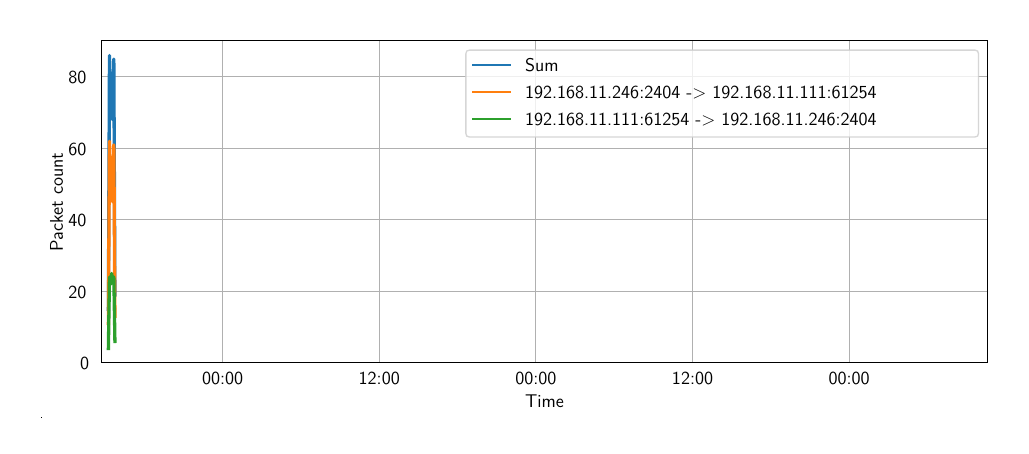
\begin{tikzpicture}
            \node(A){
            \resizebox{1\textwidth}{!}
            {
                %% Creator: Matplotlib, PGF backend
%%
%% To include the figure in your LaTeX document, write
%%   \input{<filename>.pgf}
%%
%% Make sure the required packages are loaded in your preamble
%%   \usepackage{pgf}
%%
%% Also ensure that all the required font packages are loaded; for instance,
%% the lmodern package is sometimes necessary when using math font.
%%   \usepackage{lmodern}
%%
%% Figures using additional raster images can only be included by \input if
%% they are in the same directory as the main LaTeX file. For loading figures
%% from other directories you can use the `import` package
%%   \usepackage{import}
%%
%% and then include the figures with
%%   \import{<path to file>}{<filename>.pgf}
%%
%% Matplotlib used the following preamble
%%   \usepackage{fontspec}
%%   \setmainfont{DejaVuSerif.ttf}[Path=\detokenize{/home/ankimme/fit/ibt/env/lib/python3.10/site-packages/matplotlib/mpl-data/fonts/ttf/}]
%%   \setsansfont{DejaVuSans.ttf}[Path=\detokenize{/home/ankimme/fit/ibt/env/lib/python3.10/site-packages/matplotlib/mpl-data/fonts/ttf/}]
%%   \setmonofont{DejaVuSansMono.ttf}[Path=\detokenize{/home/ankimme/fit/ibt/env/lib/python3.10/site-packages/matplotlib/mpl-data/fonts/ttf/}]
%%
\begingroup%
\makeatletter%
\begin{pgfpicture}%
\pgfpathrectangle{\pgfpointorigin}{\pgfqpoint{10.000000in}{4.000000in}}%
\pgfusepath{use as bounding box, clip}%
\begin{pgfscope}%
\pgfsetbuttcap%
\pgfsetmiterjoin%
\pgfsetlinewidth{0.000000pt}%
\definecolor{currentstroke}{rgb}{1.000000,1.000000,1.000000}%
\pgfsetstrokecolor{currentstroke}%
\pgfsetstrokeopacity{0.000000}%
\pgfsetdash{}{0pt}%
\pgfpathmoveto{\pgfqpoint{0.000000in}{0.000000in}}%
\pgfpathlineto{\pgfqpoint{10.000000in}{0.000000in}}%
\pgfpathlineto{\pgfqpoint{10.000000in}{4.000000in}}%
\pgfpathlineto{\pgfqpoint{0.000000in}{4.000000in}}%
\pgfpathlineto{\pgfqpoint{0.000000in}{0.000000in}}%
\pgfpathclose%
\pgfusepath{}%
\end{pgfscope}%
\begin{pgfscope}%
\pgfsetbuttcap%
\pgfsetmiterjoin%
\definecolor{currentfill}{rgb}{1.000000,1.000000,1.000000}%
\pgfsetfillcolor{currentfill}%
\pgfsetlinewidth{0.000000pt}%
\definecolor{currentstroke}{rgb}{0.000000,0.000000,0.000000}%
\pgfsetstrokecolor{currentstroke}%
\pgfsetstrokeopacity{0.000000}%
\pgfsetdash{}{0pt}%
\pgfpathmoveto{\pgfqpoint{0.630049in}{0.570804in}}%
\pgfpathlineto{\pgfqpoint{9.958330in}{0.570804in}}%
\pgfpathlineto{\pgfqpoint{9.958330in}{3.958330in}}%
\pgfpathlineto{\pgfqpoint{0.630049in}{3.958330in}}%
\pgfpathlineto{\pgfqpoint{0.630049in}{0.570804in}}%
\pgfpathclose%
\pgfusepath{fill}%
\end{pgfscope}%
\begin{pgfscope}%
\pgfpathrectangle{\pgfqpoint{0.630049in}{0.570804in}}{\pgfqpoint{9.328281in}{3.387526in}}%
\pgfusepath{clip}%
\pgfsetrectcap%
\pgfsetroundjoin%
\pgfsetlinewidth{0.803000pt}%
\definecolor{currentstroke}{rgb}{0.690196,0.690196,0.690196}%
\pgfsetstrokecolor{currentstroke}%
\pgfsetdash{}{0pt}%
\pgfpathmoveto{\pgfqpoint{1.907964in}{0.570804in}}%
\pgfpathlineto{\pgfqpoint{1.907964in}{3.958330in}}%
\pgfusepath{stroke}%
\end{pgfscope}%
\begin{pgfscope}%
\pgfsetbuttcap%
\pgfsetroundjoin%
\definecolor{currentfill}{rgb}{0.000000,0.000000,0.000000}%
\pgfsetfillcolor{currentfill}%
\pgfsetlinewidth{0.803000pt}%
\definecolor{currentstroke}{rgb}{0.000000,0.000000,0.000000}%
\pgfsetstrokecolor{currentstroke}%
\pgfsetdash{}{0pt}%
\pgfsys@defobject{currentmarker}{\pgfqpoint{0.000000in}{-0.048611in}}{\pgfqpoint{0.000000in}{0.000000in}}{%
\pgfpathmoveto{\pgfqpoint{0.000000in}{0.000000in}}%
\pgfpathlineto{\pgfqpoint{0.000000in}{-0.048611in}}%
\pgfusepath{stroke,fill}%
}%
\begin{pgfscope}%
\pgfsys@transformshift{1.907964in}{0.570804in}%
\pgfsys@useobject{currentmarker}{}%
\end{pgfscope}%
\end{pgfscope}%
\begin{pgfscope}%
\definecolor{textcolor}{rgb}{0.000000,0.000000,0.000000}%
\pgfsetstrokecolor{textcolor}%
\pgfsetfillcolor{textcolor}%
\pgftext[x=1.907964in,y=0.473582in,,top]{\color{textcolor}\sffamily\fontsize{14.000000}{16.800000}\selectfont 00:00}%
\end{pgfscope}%
\begin{pgfscope}%
\pgfpathrectangle{\pgfqpoint{0.630049in}{0.570804in}}{\pgfqpoint{9.328281in}{3.387526in}}%
\pgfusepath{clip}%
\pgfsetrectcap%
\pgfsetroundjoin%
\pgfsetlinewidth{0.803000pt}%
\definecolor{currentstroke}{rgb}{0.690196,0.690196,0.690196}%
\pgfsetstrokecolor{currentstroke}%
\pgfsetdash{}{0pt}%
\pgfpathmoveto{\pgfqpoint{3.556147in}{0.570804in}}%
\pgfpathlineto{\pgfqpoint{3.556147in}{3.958330in}}%
\pgfusepath{stroke}%
\end{pgfscope}%
\begin{pgfscope}%
\pgfsetbuttcap%
\pgfsetroundjoin%
\definecolor{currentfill}{rgb}{0.000000,0.000000,0.000000}%
\pgfsetfillcolor{currentfill}%
\pgfsetlinewidth{0.803000pt}%
\definecolor{currentstroke}{rgb}{0.000000,0.000000,0.000000}%
\pgfsetstrokecolor{currentstroke}%
\pgfsetdash{}{0pt}%
\pgfsys@defobject{currentmarker}{\pgfqpoint{0.000000in}{-0.048611in}}{\pgfqpoint{0.000000in}{0.000000in}}{%
\pgfpathmoveto{\pgfqpoint{0.000000in}{0.000000in}}%
\pgfpathlineto{\pgfqpoint{0.000000in}{-0.048611in}}%
\pgfusepath{stroke,fill}%
}%
\begin{pgfscope}%
\pgfsys@transformshift{3.556147in}{0.570804in}%
\pgfsys@useobject{currentmarker}{}%
\end{pgfscope}%
\end{pgfscope}%
\begin{pgfscope}%
\definecolor{textcolor}{rgb}{0.000000,0.000000,0.000000}%
\pgfsetstrokecolor{textcolor}%
\pgfsetfillcolor{textcolor}%
\pgftext[x=3.556147in,y=0.473582in,,top]{\color{textcolor}\sffamily\fontsize{14.000000}{16.800000}\selectfont 12:00}%
\end{pgfscope}%
\begin{pgfscope}%
\pgfpathrectangle{\pgfqpoint{0.630049in}{0.570804in}}{\pgfqpoint{9.328281in}{3.387526in}}%
\pgfusepath{clip}%
\pgfsetrectcap%
\pgfsetroundjoin%
\pgfsetlinewidth{0.803000pt}%
\definecolor{currentstroke}{rgb}{0.690196,0.690196,0.690196}%
\pgfsetstrokecolor{currentstroke}%
\pgfsetdash{}{0pt}%
\pgfpathmoveto{\pgfqpoint{5.204330in}{0.570804in}}%
\pgfpathlineto{\pgfqpoint{5.204330in}{3.958330in}}%
\pgfusepath{stroke}%
\end{pgfscope}%
\begin{pgfscope}%
\pgfsetbuttcap%
\pgfsetroundjoin%
\definecolor{currentfill}{rgb}{0.000000,0.000000,0.000000}%
\pgfsetfillcolor{currentfill}%
\pgfsetlinewidth{0.803000pt}%
\definecolor{currentstroke}{rgb}{0.000000,0.000000,0.000000}%
\pgfsetstrokecolor{currentstroke}%
\pgfsetdash{}{0pt}%
\pgfsys@defobject{currentmarker}{\pgfqpoint{0.000000in}{-0.048611in}}{\pgfqpoint{0.000000in}{0.000000in}}{%
\pgfpathmoveto{\pgfqpoint{0.000000in}{0.000000in}}%
\pgfpathlineto{\pgfqpoint{0.000000in}{-0.048611in}}%
\pgfusepath{stroke,fill}%
}%
\begin{pgfscope}%
\pgfsys@transformshift{5.204330in}{0.570804in}%
\pgfsys@useobject{currentmarker}{}%
\end{pgfscope}%
\end{pgfscope}%
\begin{pgfscope}%
\definecolor{textcolor}{rgb}{0.000000,0.000000,0.000000}%
\pgfsetstrokecolor{textcolor}%
\pgfsetfillcolor{textcolor}%
\pgftext[x=5.204330in,y=0.473582in,,top]{\color{textcolor}\sffamily\fontsize{14.000000}{16.800000}\selectfont 00:00}%
\end{pgfscope}%
\begin{pgfscope}%
\pgfpathrectangle{\pgfqpoint{0.630049in}{0.570804in}}{\pgfqpoint{9.328281in}{3.387526in}}%
\pgfusepath{clip}%
\pgfsetrectcap%
\pgfsetroundjoin%
\pgfsetlinewidth{0.803000pt}%
\definecolor{currentstroke}{rgb}{0.690196,0.690196,0.690196}%
\pgfsetstrokecolor{currentstroke}%
\pgfsetdash{}{0pt}%
\pgfpathmoveto{\pgfqpoint{6.852513in}{0.570804in}}%
\pgfpathlineto{\pgfqpoint{6.852513in}{3.958330in}}%
\pgfusepath{stroke}%
\end{pgfscope}%
\begin{pgfscope}%
\pgfsetbuttcap%
\pgfsetroundjoin%
\definecolor{currentfill}{rgb}{0.000000,0.000000,0.000000}%
\pgfsetfillcolor{currentfill}%
\pgfsetlinewidth{0.803000pt}%
\definecolor{currentstroke}{rgb}{0.000000,0.000000,0.000000}%
\pgfsetstrokecolor{currentstroke}%
\pgfsetdash{}{0pt}%
\pgfsys@defobject{currentmarker}{\pgfqpoint{0.000000in}{-0.048611in}}{\pgfqpoint{0.000000in}{0.000000in}}{%
\pgfpathmoveto{\pgfqpoint{0.000000in}{0.000000in}}%
\pgfpathlineto{\pgfqpoint{0.000000in}{-0.048611in}}%
\pgfusepath{stroke,fill}%
}%
\begin{pgfscope}%
\pgfsys@transformshift{6.852513in}{0.570804in}%
\pgfsys@useobject{currentmarker}{}%
\end{pgfscope}%
\end{pgfscope}%
\begin{pgfscope}%
\definecolor{textcolor}{rgb}{0.000000,0.000000,0.000000}%
\pgfsetstrokecolor{textcolor}%
\pgfsetfillcolor{textcolor}%
\pgftext[x=6.852513in,y=0.473582in,,top]{\color{textcolor}\sffamily\fontsize{14.000000}{16.800000}\selectfont 12:00}%
\end{pgfscope}%
\begin{pgfscope}%
\pgfpathrectangle{\pgfqpoint{0.630049in}{0.570804in}}{\pgfqpoint{9.328281in}{3.387526in}}%
\pgfusepath{clip}%
\pgfsetrectcap%
\pgfsetroundjoin%
\pgfsetlinewidth{0.803000pt}%
\definecolor{currentstroke}{rgb}{0.690196,0.690196,0.690196}%
\pgfsetstrokecolor{currentstroke}%
\pgfsetdash{}{0pt}%
\pgfpathmoveto{\pgfqpoint{8.500696in}{0.570804in}}%
\pgfpathlineto{\pgfqpoint{8.500696in}{3.958330in}}%
\pgfusepath{stroke}%
\end{pgfscope}%
\begin{pgfscope}%
\pgfsetbuttcap%
\pgfsetroundjoin%
\definecolor{currentfill}{rgb}{0.000000,0.000000,0.000000}%
\pgfsetfillcolor{currentfill}%
\pgfsetlinewidth{0.803000pt}%
\definecolor{currentstroke}{rgb}{0.000000,0.000000,0.000000}%
\pgfsetstrokecolor{currentstroke}%
\pgfsetdash{}{0pt}%
\pgfsys@defobject{currentmarker}{\pgfqpoint{0.000000in}{-0.048611in}}{\pgfqpoint{0.000000in}{0.000000in}}{%
\pgfpathmoveto{\pgfqpoint{0.000000in}{0.000000in}}%
\pgfpathlineto{\pgfqpoint{0.000000in}{-0.048611in}}%
\pgfusepath{stroke,fill}%
}%
\begin{pgfscope}%
\pgfsys@transformshift{8.500696in}{0.570804in}%
\pgfsys@useobject{currentmarker}{}%
\end{pgfscope}%
\end{pgfscope}%
\begin{pgfscope}%
\definecolor{textcolor}{rgb}{0.000000,0.000000,0.000000}%
\pgfsetstrokecolor{textcolor}%
\pgfsetfillcolor{textcolor}%
\pgftext[x=8.500696in,y=0.473582in,,top]{\color{textcolor}\sffamily\fontsize{14.000000}{16.800000}\selectfont 00:00}%
\end{pgfscope}%
\begin{pgfscope}%
\definecolor{textcolor}{rgb}{0.000000,0.000000,0.000000}%
\pgfsetstrokecolor{textcolor}%
\pgfsetfillcolor{textcolor}%
\pgftext[x=5.294189in,y=0.229848in,,top]{\color{textcolor}\sffamily\fontsize{14.000000}{16.800000}\selectfont Time}%
\end{pgfscope}%
\begin{pgfscope}%
\pgfpathrectangle{\pgfqpoint{0.630049in}{0.570804in}}{\pgfqpoint{9.328281in}{3.387526in}}%
\pgfusepath{clip}%
\pgfsetrectcap%
\pgfsetroundjoin%
\pgfsetlinewidth{0.803000pt}%
\definecolor{currentstroke}{rgb}{0.690196,0.690196,0.690196}%
\pgfsetstrokecolor{currentstroke}%
\pgfsetdash{}{0pt}%
\pgfpathmoveto{\pgfqpoint{0.630049in}{0.570804in}}%
\pgfpathlineto{\pgfqpoint{9.958330in}{0.570804in}}%
\pgfusepath{stroke}%
\end{pgfscope}%
\begin{pgfscope}%
\pgfsetbuttcap%
\pgfsetroundjoin%
\definecolor{currentfill}{rgb}{0.000000,0.000000,0.000000}%
\pgfsetfillcolor{currentfill}%
\pgfsetlinewidth{0.803000pt}%
\definecolor{currentstroke}{rgb}{0.000000,0.000000,0.000000}%
\pgfsetstrokecolor{currentstroke}%
\pgfsetdash{}{0pt}%
\pgfsys@defobject{currentmarker}{\pgfqpoint{-0.048611in}{0.000000in}}{\pgfqpoint{-0.000000in}{0.000000in}}{%
\pgfpathmoveto{\pgfqpoint{-0.000000in}{0.000000in}}%
\pgfpathlineto{\pgfqpoint{-0.048611in}{0.000000in}}%
\pgfusepath{stroke,fill}%
}%
\begin{pgfscope}%
\pgfsys@transformshift{0.630049in}{0.570804in}%
\pgfsys@useobject{currentmarker}{}%
\end{pgfscope}%
\end{pgfscope}%
\begin{pgfscope}%
\definecolor{textcolor}{rgb}{0.000000,0.000000,0.000000}%
\pgfsetstrokecolor{textcolor}%
\pgfsetfillcolor{textcolor}%
\pgftext[x=0.409115in, y=0.496938in, left, base]{\color{textcolor}\sffamily\fontsize{14.000000}{16.800000}\selectfont 0}%
\end{pgfscope}%
\begin{pgfscope}%
\pgfpathrectangle{\pgfqpoint{0.630049in}{0.570804in}}{\pgfqpoint{9.328281in}{3.387526in}}%
\pgfusepath{clip}%
\pgfsetrectcap%
\pgfsetroundjoin%
\pgfsetlinewidth{0.803000pt}%
\definecolor{currentstroke}{rgb}{0.690196,0.690196,0.690196}%
\pgfsetstrokecolor{currentstroke}%
\pgfsetdash{}{0pt}%
\pgfpathmoveto{\pgfqpoint{0.630049in}{1.322752in}}%
\pgfpathlineto{\pgfqpoint{9.958330in}{1.322752in}}%
\pgfusepath{stroke}%
\end{pgfscope}%
\begin{pgfscope}%
\pgfsetbuttcap%
\pgfsetroundjoin%
\definecolor{currentfill}{rgb}{0.000000,0.000000,0.000000}%
\pgfsetfillcolor{currentfill}%
\pgfsetlinewidth{0.803000pt}%
\definecolor{currentstroke}{rgb}{0.000000,0.000000,0.000000}%
\pgfsetstrokecolor{currentstroke}%
\pgfsetdash{}{0pt}%
\pgfsys@defobject{currentmarker}{\pgfqpoint{-0.048611in}{0.000000in}}{\pgfqpoint{-0.000000in}{0.000000in}}{%
\pgfpathmoveto{\pgfqpoint{-0.000000in}{0.000000in}}%
\pgfpathlineto{\pgfqpoint{-0.048611in}{0.000000in}}%
\pgfusepath{stroke,fill}%
}%
\begin{pgfscope}%
\pgfsys@transformshift{0.630049in}{1.322752in}%
\pgfsys@useobject{currentmarker}{}%
\end{pgfscope}%
\end{pgfscope}%
\begin{pgfscope}%
\definecolor{textcolor}{rgb}{0.000000,0.000000,0.000000}%
\pgfsetstrokecolor{textcolor}%
\pgfsetfillcolor{textcolor}%
\pgftext[x=0.285404in, y=1.248886in, left, base]{\color{textcolor}\sffamily\fontsize{14.000000}{16.800000}\selectfont 20}%
\end{pgfscope}%
\begin{pgfscope}%
\pgfpathrectangle{\pgfqpoint{0.630049in}{0.570804in}}{\pgfqpoint{9.328281in}{3.387526in}}%
\pgfusepath{clip}%
\pgfsetrectcap%
\pgfsetroundjoin%
\pgfsetlinewidth{0.803000pt}%
\definecolor{currentstroke}{rgb}{0.690196,0.690196,0.690196}%
\pgfsetstrokecolor{currentstroke}%
\pgfsetdash{}{0pt}%
\pgfpathmoveto{\pgfqpoint{0.630049in}{2.074700in}}%
\pgfpathlineto{\pgfqpoint{9.958330in}{2.074700in}}%
\pgfusepath{stroke}%
\end{pgfscope}%
\begin{pgfscope}%
\pgfsetbuttcap%
\pgfsetroundjoin%
\definecolor{currentfill}{rgb}{0.000000,0.000000,0.000000}%
\pgfsetfillcolor{currentfill}%
\pgfsetlinewidth{0.803000pt}%
\definecolor{currentstroke}{rgb}{0.000000,0.000000,0.000000}%
\pgfsetstrokecolor{currentstroke}%
\pgfsetdash{}{0pt}%
\pgfsys@defobject{currentmarker}{\pgfqpoint{-0.048611in}{0.000000in}}{\pgfqpoint{-0.000000in}{0.000000in}}{%
\pgfpathmoveto{\pgfqpoint{-0.000000in}{0.000000in}}%
\pgfpathlineto{\pgfqpoint{-0.048611in}{0.000000in}}%
\pgfusepath{stroke,fill}%
}%
\begin{pgfscope}%
\pgfsys@transformshift{0.630049in}{2.074700in}%
\pgfsys@useobject{currentmarker}{}%
\end{pgfscope}%
\end{pgfscope}%
\begin{pgfscope}%
\definecolor{textcolor}{rgb}{0.000000,0.000000,0.000000}%
\pgfsetstrokecolor{textcolor}%
\pgfsetfillcolor{textcolor}%
\pgftext[x=0.285404in, y=2.000834in, left, base]{\color{textcolor}\sffamily\fontsize{14.000000}{16.800000}\selectfont 40}%
\end{pgfscope}%
\begin{pgfscope}%
\pgfpathrectangle{\pgfqpoint{0.630049in}{0.570804in}}{\pgfqpoint{9.328281in}{3.387526in}}%
\pgfusepath{clip}%
\pgfsetrectcap%
\pgfsetroundjoin%
\pgfsetlinewidth{0.803000pt}%
\definecolor{currentstroke}{rgb}{0.690196,0.690196,0.690196}%
\pgfsetstrokecolor{currentstroke}%
\pgfsetdash{}{0pt}%
\pgfpathmoveto{\pgfqpoint{0.630049in}{2.826648in}}%
\pgfpathlineto{\pgfqpoint{9.958330in}{2.826648in}}%
\pgfusepath{stroke}%
\end{pgfscope}%
\begin{pgfscope}%
\pgfsetbuttcap%
\pgfsetroundjoin%
\definecolor{currentfill}{rgb}{0.000000,0.000000,0.000000}%
\pgfsetfillcolor{currentfill}%
\pgfsetlinewidth{0.803000pt}%
\definecolor{currentstroke}{rgb}{0.000000,0.000000,0.000000}%
\pgfsetstrokecolor{currentstroke}%
\pgfsetdash{}{0pt}%
\pgfsys@defobject{currentmarker}{\pgfqpoint{-0.048611in}{0.000000in}}{\pgfqpoint{-0.000000in}{0.000000in}}{%
\pgfpathmoveto{\pgfqpoint{-0.000000in}{0.000000in}}%
\pgfpathlineto{\pgfqpoint{-0.048611in}{0.000000in}}%
\pgfusepath{stroke,fill}%
}%
\begin{pgfscope}%
\pgfsys@transformshift{0.630049in}{2.826648in}%
\pgfsys@useobject{currentmarker}{}%
\end{pgfscope}%
\end{pgfscope}%
\begin{pgfscope}%
\definecolor{textcolor}{rgb}{0.000000,0.000000,0.000000}%
\pgfsetstrokecolor{textcolor}%
\pgfsetfillcolor{textcolor}%
\pgftext[x=0.285404in, y=2.752782in, left, base]{\color{textcolor}\sffamily\fontsize{14.000000}{16.800000}\selectfont 60}%
\end{pgfscope}%
\begin{pgfscope}%
\pgfpathrectangle{\pgfqpoint{0.630049in}{0.570804in}}{\pgfqpoint{9.328281in}{3.387526in}}%
\pgfusepath{clip}%
\pgfsetrectcap%
\pgfsetroundjoin%
\pgfsetlinewidth{0.803000pt}%
\definecolor{currentstroke}{rgb}{0.690196,0.690196,0.690196}%
\pgfsetstrokecolor{currentstroke}%
\pgfsetdash{}{0pt}%
\pgfpathmoveto{\pgfqpoint{0.630049in}{3.578596in}}%
\pgfpathlineto{\pgfqpoint{9.958330in}{3.578596in}}%
\pgfusepath{stroke}%
\end{pgfscope}%
\begin{pgfscope}%
\pgfsetbuttcap%
\pgfsetroundjoin%
\definecolor{currentfill}{rgb}{0.000000,0.000000,0.000000}%
\pgfsetfillcolor{currentfill}%
\pgfsetlinewidth{0.803000pt}%
\definecolor{currentstroke}{rgb}{0.000000,0.000000,0.000000}%
\pgfsetstrokecolor{currentstroke}%
\pgfsetdash{}{0pt}%
\pgfsys@defobject{currentmarker}{\pgfqpoint{-0.048611in}{0.000000in}}{\pgfqpoint{-0.000000in}{0.000000in}}{%
\pgfpathmoveto{\pgfqpoint{-0.000000in}{0.000000in}}%
\pgfpathlineto{\pgfqpoint{-0.048611in}{0.000000in}}%
\pgfusepath{stroke,fill}%
}%
\begin{pgfscope}%
\pgfsys@transformshift{0.630049in}{3.578596in}%
\pgfsys@useobject{currentmarker}{}%
\end{pgfscope}%
\end{pgfscope}%
\begin{pgfscope}%
\definecolor{textcolor}{rgb}{0.000000,0.000000,0.000000}%
\pgfsetstrokecolor{textcolor}%
\pgfsetfillcolor{textcolor}%
\pgftext[x=0.285404in, y=3.504730in, left, base]{\color{textcolor}\sffamily\fontsize{14.000000}{16.800000}\selectfont 80}%
\end{pgfscope}%
\begin{pgfscope}%
\definecolor{textcolor}{rgb}{0.000000,0.000000,0.000000}%
\pgfsetstrokecolor{textcolor}%
\pgfsetfillcolor{textcolor}%
\pgftext[x=0.229848in,y=2.264567in,,bottom,rotate=90.000000]{\color{textcolor}\sffamily\fontsize{14.000000}{16.800000}\selectfont Packet count}%
\end{pgfscope}%
\begin{pgfscope}%
\pgfpathrectangle{\pgfqpoint{0.630049in}{0.570804in}}{\pgfqpoint{9.328281in}{3.387526in}}%
\pgfusepath{clip}%
\pgfsetrectcap%
\pgfsetroundjoin%
\pgfsetlinewidth{2.509375pt}%
\definecolor{currentstroke}{rgb}{0.121569,0.466667,0.705882}%
\pgfsetstrokecolor{currentstroke}%
\pgfsetdash{}{0pt}%
\pgfpathmoveto{\pgfqpoint{0.706164in}{1.134765in}}%
\pgfpathlineto{\pgfqpoint{0.717609in}{3.804181in}}%
\pgfpathlineto{\pgfqpoint{0.729055in}{3.277817in}}%
\pgfpathlineto{\pgfqpoint{0.740501in}{3.616194in}}%
\pgfpathlineto{\pgfqpoint{0.751946in}{3.127427in}}%
\pgfpathlineto{\pgfqpoint{0.763392in}{3.766583in}}%
\pgfpathlineto{\pgfqpoint{0.774838in}{1.285155in}}%
\pgfusepath{stroke}%
\end{pgfscope}%
\begin{pgfscope}%
\pgfpathrectangle{\pgfqpoint{0.630049in}{0.570804in}}{\pgfqpoint{9.328281in}{3.387526in}}%
\pgfusepath{clip}%
\pgfsetrectcap%
\pgfsetroundjoin%
\pgfsetlinewidth{2.509375pt}%
\definecolor{currentstroke}{rgb}{1.000000,0.498039,0.054902}%
\pgfsetstrokecolor{currentstroke}%
\pgfsetdash{}{0pt}%
\pgfpathmoveto{\pgfqpoint{0.706164in}{0.984375in}}%
\pgfpathlineto{\pgfqpoint{0.717609in}{2.901843in}}%
\pgfpathlineto{\pgfqpoint{0.729055in}{2.450674in}}%
\pgfpathlineto{\pgfqpoint{0.740501in}{2.676259in}}%
\pgfpathlineto{\pgfqpoint{0.751946in}{2.262687in}}%
\pgfpathlineto{\pgfqpoint{0.763392in}{2.864246in}}%
\pgfpathlineto{\pgfqpoint{0.774838in}{1.059570in}}%
\pgfusepath{stroke}%
\end{pgfscope}%
\begin{pgfscope}%
\pgfpathrectangle{\pgfqpoint{0.630049in}{0.570804in}}{\pgfqpoint{9.328281in}{3.387526in}}%
\pgfusepath{clip}%
\pgfsetrectcap%
\pgfsetroundjoin%
\pgfsetlinewidth{2.509375pt}%
\definecolor{currentstroke}{rgb}{0.172549,0.627451,0.172549}%
\pgfsetstrokecolor{currentstroke}%
\pgfsetdash{}{0pt}%
\pgfpathmoveto{\pgfqpoint{0.706164in}{0.721194in}}%
\pgfpathlineto{\pgfqpoint{0.717609in}{1.473142in}}%
\pgfpathlineto{\pgfqpoint{0.729055in}{1.397947in}}%
\pgfpathlineto{\pgfqpoint{0.740501in}{1.510739in}}%
\pgfpathlineto{\pgfqpoint{0.751946in}{1.435544in}}%
\pgfpathlineto{\pgfqpoint{0.763392in}{1.473142in}}%
\pgfpathlineto{\pgfqpoint{0.774838in}{0.796388in}}%
\pgfusepath{stroke}%
\end{pgfscope}%
\begin{pgfscope}%
\pgfsetrectcap%
\pgfsetmiterjoin%
\pgfsetlinewidth{0.803000pt}%
\definecolor{currentstroke}{rgb}{0.000000,0.000000,0.000000}%
\pgfsetstrokecolor{currentstroke}%
\pgfsetdash{}{0pt}%
\pgfpathmoveto{\pgfqpoint{0.630049in}{0.570804in}}%
\pgfpathlineto{\pgfqpoint{0.630049in}{3.958330in}}%
\pgfusepath{stroke}%
\end{pgfscope}%
\begin{pgfscope}%
\pgfsetrectcap%
\pgfsetmiterjoin%
\pgfsetlinewidth{0.803000pt}%
\definecolor{currentstroke}{rgb}{0.000000,0.000000,0.000000}%
\pgfsetstrokecolor{currentstroke}%
\pgfsetdash{}{0pt}%
\pgfpathmoveto{\pgfqpoint{9.958330in}{0.570804in}}%
\pgfpathlineto{\pgfqpoint{9.958330in}{3.958330in}}%
\pgfusepath{stroke}%
\end{pgfscope}%
\begin{pgfscope}%
\pgfsetrectcap%
\pgfsetmiterjoin%
\pgfsetlinewidth{0.803000pt}%
\definecolor{currentstroke}{rgb}{0.000000,0.000000,0.000000}%
\pgfsetstrokecolor{currentstroke}%
\pgfsetdash{}{0pt}%
\pgfpathmoveto{\pgfqpoint{0.630049in}{0.570804in}}%
\pgfpathlineto{\pgfqpoint{9.958330in}{0.570804in}}%
\pgfusepath{stroke}%
\end{pgfscope}%
\begin{pgfscope}%
\pgfsetrectcap%
\pgfsetmiterjoin%
\pgfsetlinewidth{0.803000pt}%
\definecolor{currentstroke}{rgb}{0.000000,0.000000,0.000000}%
\pgfsetstrokecolor{currentstroke}%
\pgfsetdash{}{0pt}%
\pgfpathmoveto{\pgfqpoint{0.630049in}{3.958330in}}%
\pgfpathlineto{\pgfqpoint{9.958330in}{3.958330in}}%
\pgfusepath{stroke}%
\end{pgfscope}%
\begin{pgfscope}%
\pgfsetbuttcap%
\pgfsetmiterjoin%
\definecolor{currentfill}{rgb}{1.000000,1.000000,1.000000}%
\pgfsetfillcolor{currentfill}%
\pgfsetfillopacity{0.800000}%
\pgfsetlinewidth{1.003750pt}%
\definecolor{currentstroke}{rgb}{0.800000,0.800000,0.800000}%
\pgfsetstrokecolor{currentstroke}%
\pgfsetstrokeopacity{0.800000}%
\pgfsetdash{}{0pt}%
\pgfpathmoveto{\pgfqpoint{4.506366in}{2.946574in}}%
\pgfpathlineto{\pgfqpoint{9.822219in}{2.946574in}}%
\pgfpathquadraticcurveto{\pgfqpoint{9.861108in}{2.946574in}}{\pgfqpoint{9.861108in}{2.985463in}}%
\pgfpathlineto{\pgfqpoint{9.861108in}{3.822219in}}%
\pgfpathquadraticcurveto{\pgfqpoint{9.861108in}{3.861108in}}{\pgfqpoint{9.822219in}{3.861108in}}%
\pgfpathlineto{\pgfqpoint{4.506366in}{3.861108in}}%
\pgfpathquadraticcurveto{\pgfqpoint{4.467477in}{3.861108in}}{\pgfqpoint{4.467477in}{3.822219in}}%
\pgfpathlineto{\pgfqpoint{4.467477in}{2.985463in}}%
\pgfpathquadraticcurveto{\pgfqpoint{4.467477in}{2.946574in}}{\pgfqpoint{4.506366in}{2.946574in}}%
\pgfpathlineto{\pgfqpoint{4.506366in}{2.946574in}}%
\pgfpathclose%
\pgfusepath{stroke,fill}%
\end{pgfscope}%
\begin{pgfscope}%
\pgfsetrectcap%
\pgfsetroundjoin%
\pgfsetlinewidth{1.505625pt}%
\definecolor{currentstroke}{rgb}{0.121569,0.466667,0.705882}%
\pgfsetstrokecolor{currentstroke}%
\pgfsetdash{}{0pt}%
\pgfpathmoveto{\pgfqpoint{4.545255in}{3.703653in}}%
\pgfpathlineto{\pgfqpoint{4.739699in}{3.703653in}}%
\pgfpathlineto{\pgfqpoint{4.934144in}{3.703653in}}%
\pgfusepath{stroke}%
\end{pgfscope}%
\begin{pgfscope}%
\definecolor{textcolor}{rgb}{0.000000,0.000000,0.000000}%
\pgfsetstrokecolor{textcolor}%
\pgfsetfillcolor{textcolor}%
\pgftext[x=5.089699in,y=3.635598in,left,base]{\color{textcolor}\sffamily\fontsize{14.000000}{16.800000}\selectfont Sum}%
\end{pgfscope}%
\begin{pgfscope}%
\pgfsetrectcap%
\pgfsetroundjoin%
\pgfsetlinewidth{1.505625pt}%
\definecolor{currentstroke}{rgb}{1.000000,0.498039,0.054902}%
\pgfsetstrokecolor{currentstroke}%
\pgfsetdash{}{0pt}%
\pgfpathmoveto{\pgfqpoint{4.545255in}{3.418253in}}%
\pgfpathlineto{\pgfqpoint{4.739699in}{3.418253in}}%
\pgfpathlineto{\pgfqpoint{4.934144in}{3.418253in}}%
\pgfusepath{stroke}%
\end{pgfscope}%
\begin{pgfscope}%
\definecolor{textcolor}{rgb}{0.000000,0.000000,0.000000}%
\pgfsetstrokecolor{textcolor}%
\pgfsetfillcolor{textcolor}%
\pgftext[x=5.089699in,y=3.350198in,left,base]{\color{textcolor}\sffamily\fontsize{14.000000}{16.800000}\selectfont 192.168.11.246:2404 -> 192.168.11.111:61254}%
\end{pgfscope}%
\begin{pgfscope}%
\pgfsetrectcap%
\pgfsetroundjoin%
\pgfsetlinewidth{1.505625pt}%
\definecolor{currentstroke}{rgb}{0.172549,0.627451,0.172549}%
\pgfsetstrokecolor{currentstroke}%
\pgfsetdash{}{0pt}%
\pgfpathmoveto{\pgfqpoint{4.545255in}{3.132853in}}%
\pgfpathlineto{\pgfqpoint{4.739699in}{3.132853in}}%
\pgfpathlineto{\pgfqpoint{4.934144in}{3.132853in}}%
\pgfusepath{stroke}%
\end{pgfscope}%
\begin{pgfscope}%
\definecolor{textcolor}{rgb}{0.000000,0.000000,0.000000}%
\pgfsetstrokecolor{textcolor}%
\pgfsetfillcolor{textcolor}%
\pgftext[x=5.089699in,y=3.064797in,left,base]{\color{textcolor}\sffamily\fontsize{14.000000}{16.800000}\selectfont 192.168.11.111:61254 -> 192.168.11.246:2404}%
\end{pgfscope}%
\end{pgfpicture}%
\makeatother%
\endgroup%

            }
        };
        \end{tikzpicture}  
        \captionsetup{width=0.9\linewidth}
        \caption{Komunikace podvržené řídící stanice.}
        \label{fig:rogue_attacker}
    \end{subfigure}
    
    \begin{subfigure}{\textwidth}
        \centering
        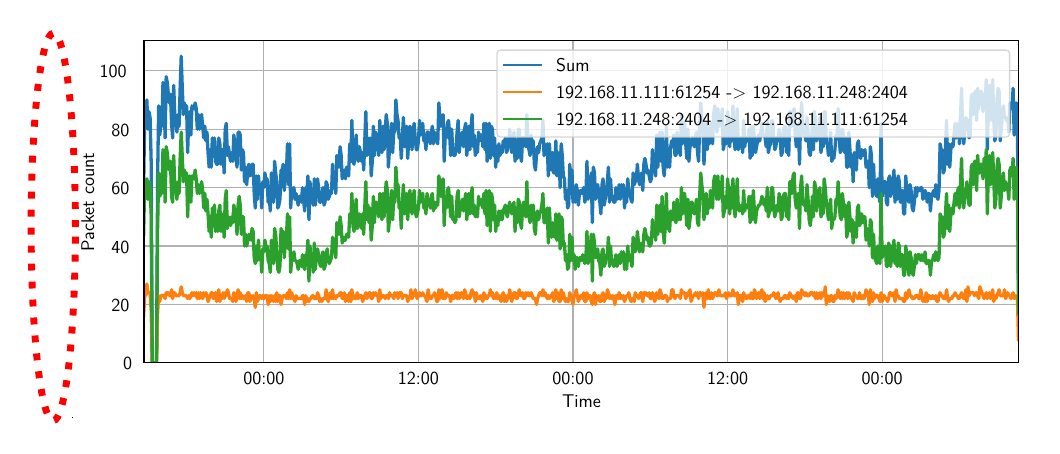
\begin{tikzpicture}
            \node(A){   
            \resizebox{1\textwidth}{!}
                {
                    %% Creator: Matplotlib, PGF backend
%%
%% To include the figure in your LaTeX document, write
%%   \input{<filename>.pgf}
%%
%% Make sure the required packages are loaded in your preamble
%%   \usepackage{pgf}
%%
%% Also ensure that all the required font packages are loaded; for instance,
%% the lmodern package is sometimes necessary when using math font.
%%   \usepackage{lmodern}
%%
%% Figures using additional raster images can only be included by \input if
%% they are in the same directory as the main LaTeX file. For loading figures
%% from other directories you can use the `import` package
%%   \usepackage{import}
%%
%% and then include the figures with
%%   \import{<path to file>}{<filename>.pgf}
%%
%% Matplotlib used the following preamble
%%   \usepackage{fontspec}
%%   \setmainfont{DejaVuSerif.ttf}[Path=\detokenize{/home/ankimme/fit/ibt/env/lib/python3.10/site-packages/matplotlib/mpl-data/fonts/ttf/}]
%%   \setsansfont{DejaVuSans.ttf}[Path=\detokenize{/home/ankimme/fit/ibt/env/lib/python3.10/site-packages/matplotlib/mpl-data/fonts/ttf/}]
%%   \setmonofont{DejaVuSansMono.ttf}[Path=\detokenize{/home/ankimme/fit/ibt/env/lib/python3.10/site-packages/matplotlib/mpl-data/fonts/ttf/}]
%%
\begingroup%
\makeatletter%
\begin{pgfpicture}%
\pgfpathrectangle{\pgfpointorigin}{\pgfqpoint{10.000000in}{4.000000in}}%
\pgfusepath{use as bounding box, clip}%
\begin{pgfscope}%
\pgfsetbuttcap%
\pgfsetmiterjoin%
\pgfsetlinewidth{0.000000pt}%
\definecolor{currentstroke}{rgb}{1.000000,1.000000,1.000000}%
\pgfsetstrokecolor{currentstroke}%
\pgfsetstrokeopacity{0.000000}%
\pgfsetdash{}{0pt}%
\pgfpathmoveto{\pgfqpoint{0.000000in}{0.000000in}}%
\pgfpathlineto{\pgfqpoint{10.000000in}{0.000000in}}%
\pgfpathlineto{\pgfqpoint{10.000000in}{4.000000in}}%
\pgfpathlineto{\pgfqpoint{0.000000in}{4.000000in}}%
\pgfpathlineto{\pgfqpoint{0.000000in}{0.000000in}}%
\pgfpathclose%
\pgfusepath{}%
\end{pgfscope}%
\begin{pgfscope}%
\pgfsetbuttcap%
\pgfsetmiterjoin%
\definecolor{currentfill}{rgb}{1.000000,1.000000,1.000000}%
\pgfsetfillcolor{currentfill}%
\pgfsetlinewidth{0.000000pt}%
\definecolor{currentstroke}{rgb}{0.000000,0.000000,0.000000}%
\pgfsetstrokecolor{currentstroke}%
\pgfsetstrokeopacity{0.000000}%
\pgfsetdash{}{0pt}%
\pgfpathmoveto{\pgfqpoint{0.753760in}{0.570804in}}%
\pgfpathlineto{\pgfqpoint{9.958330in}{0.570804in}}%
\pgfpathlineto{\pgfqpoint{9.958330in}{3.958330in}}%
\pgfpathlineto{\pgfqpoint{0.753760in}{3.958330in}}%
\pgfpathlineto{\pgfqpoint{0.753760in}{0.570804in}}%
\pgfpathclose%
\pgfusepath{fill}%
\end{pgfscope}%
\begin{pgfscope}%
\pgfpathrectangle{\pgfqpoint{0.753760in}{0.570804in}}{\pgfqpoint{9.204570in}{3.387526in}}%
\pgfusepath{clip}%
\pgfsetrectcap%
\pgfsetroundjoin%
\pgfsetlinewidth{0.803000pt}%
\definecolor{currentstroke}{rgb}{0.690196,0.690196,0.690196}%
\pgfsetstrokecolor{currentstroke}%
\pgfsetdash{}{0pt}%
\pgfpathmoveto{\pgfqpoint{2.014728in}{0.570804in}}%
\pgfpathlineto{\pgfqpoint{2.014728in}{3.958330in}}%
\pgfusepath{stroke}%
\end{pgfscope}%
\begin{pgfscope}%
\pgfsetbuttcap%
\pgfsetroundjoin%
\definecolor{currentfill}{rgb}{0.000000,0.000000,0.000000}%
\pgfsetfillcolor{currentfill}%
\pgfsetlinewidth{0.803000pt}%
\definecolor{currentstroke}{rgb}{0.000000,0.000000,0.000000}%
\pgfsetstrokecolor{currentstroke}%
\pgfsetdash{}{0pt}%
\pgfsys@defobject{currentmarker}{\pgfqpoint{0.000000in}{-0.048611in}}{\pgfqpoint{0.000000in}{0.000000in}}{%
\pgfpathmoveto{\pgfqpoint{0.000000in}{0.000000in}}%
\pgfpathlineto{\pgfqpoint{0.000000in}{-0.048611in}}%
\pgfusepath{stroke,fill}%
}%
\begin{pgfscope}%
\pgfsys@transformshift{2.014728in}{0.570804in}%
\pgfsys@useobject{currentmarker}{}%
\end{pgfscope}%
\end{pgfscope}%
\begin{pgfscope}%
\definecolor{textcolor}{rgb}{0.000000,0.000000,0.000000}%
\pgfsetstrokecolor{textcolor}%
\pgfsetfillcolor{textcolor}%
\pgftext[x=2.014728in,y=0.473582in,,top]{\color{textcolor}\sffamily\fontsize{14.000000}{16.800000}\selectfont 00:00}%
\end{pgfscope}%
\begin{pgfscope}%
\pgfpathrectangle{\pgfqpoint{0.753760in}{0.570804in}}{\pgfqpoint{9.204570in}{3.387526in}}%
\pgfusepath{clip}%
\pgfsetrectcap%
\pgfsetroundjoin%
\pgfsetlinewidth{0.803000pt}%
\definecolor{currentstroke}{rgb}{0.690196,0.690196,0.690196}%
\pgfsetstrokecolor{currentstroke}%
\pgfsetdash{}{0pt}%
\pgfpathmoveto{\pgfqpoint{3.641053in}{0.570804in}}%
\pgfpathlineto{\pgfqpoint{3.641053in}{3.958330in}}%
\pgfusepath{stroke}%
\end{pgfscope}%
\begin{pgfscope}%
\pgfsetbuttcap%
\pgfsetroundjoin%
\definecolor{currentfill}{rgb}{0.000000,0.000000,0.000000}%
\pgfsetfillcolor{currentfill}%
\pgfsetlinewidth{0.803000pt}%
\definecolor{currentstroke}{rgb}{0.000000,0.000000,0.000000}%
\pgfsetstrokecolor{currentstroke}%
\pgfsetdash{}{0pt}%
\pgfsys@defobject{currentmarker}{\pgfqpoint{0.000000in}{-0.048611in}}{\pgfqpoint{0.000000in}{0.000000in}}{%
\pgfpathmoveto{\pgfqpoint{0.000000in}{0.000000in}}%
\pgfpathlineto{\pgfqpoint{0.000000in}{-0.048611in}}%
\pgfusepath{stroke,fill}%
}%
\begin{pgfscope}%
\pgfsys@transformshift{3.641053in}{0.570804in}%
\pgfsys@useobject{currentmarker}{}%
\end{pgfscope}%
\end{pgfscope}%
\begin{pgfscope}%
\definecolor{textcolor}{rgb}{0.000000,0.000000,0.000000}%
\pgfsetstrokecolor{textcolor}%
\pgfsetfillcolor{textcolor}%
\pgftext[x=3.641053in,y=0.473582in,,top]{\color{textcolor}\sffamily\fontsize{14.000000}{16.800000}\selectfont 12:00}%
\end{pgfscope}%
\begin{pgfscope}%
\pgfpathrectangle{\pgfqpoint{0.753760in}{0.570804in}}{\pgfqpoint{9.204570in}{3.387526in}}%
\pgfusepath{clip}%
\pgfsetrectcap%
\pgfsetroundjoin%
\pgfsetlinewidth{0.803000pt}%
\definecolor{currentstroke}{rgb}{0.690196,0.690196,0.690196}%
\pgfsetstrokecolor{currentstroke}%
\pgfsetdash{}{0pt}%
\pgfpathmoveto{\pgfqpoint{5.267377in}{0.570804in}}%
\pgfpathlineto{\pgfqpoint{5.267377in}{3.958330in}}%
\pgfusepath{stroke}%
\end{pgfscope}%
\begin{pgfscope}%
\pgfsetbuttcap%
\pgfsetroundjoin%
\definecolor{currentfill}{rgb}{0.000000,0.000000,0.000000}%
\pgfsetfillcolor{currentfill}%
\pgfsetlinewidth{0.803000pt}%
\definecolor{currentstroke}{rgb}{0.000000,0.000000,0.000000}%
\pgfsetstrokecolor{currentstroke}%
\pgfsetdash{}{0pt}%
\pgfsys@defobject{currentmarker}{\pgfqpoint{0.000000in}{-0.048611in}}{\pgfqpoint{0.000000in}{0.000000in}}{%
\pgfpathmoveto{\pgfqpoint{0.000000in}{0.000000in}}%
\pgfpathlineto{\pgfqpoint{0.000000in}{-0.048611in}}%
\pgfusepath{stroke,fill}%
}%
\begin{pgfscope}%
\pgfsys@transformshift{5.267377in}{0.570804in}%
\pgfsys@useobject{currentmarker}{}%
\end{pgfscope}%
\end{pgfscope}%
\begin{pgfscope}%
\definecolor{textcolor}{rgb}{0.000000,0.000000,0.000000}%
\pgfsetstrokecolor{textcolor}%
\pgfsetfillcolor{textcolor}%
\pgftext[x=5.267377in,y=0.473582in,,top]{\color{textcolor}\sffamily\fontsize{14.000000}{16.800000}\selectfont 00:00}%
\end{pgfscope}%
\begin{pgfscope}%
\pgfpathrectangle{\pgfqpoint{0.753760in}{0.570804in}}{\pgfqpoint{9.204570in}{3.387526in}}%
\pgfusepath{clip}%
\pgfsetrectcap%
\pgfsetroundjoin%
\pgfsetlinewidth{0.803000pt}%
\definecolor{currentstroke}{rgb}{0.690196,0.690196,0.690196}%
\pgfsetstrokecolor{currentstroke}%
\pgfsetdash{}{0pt}%
\pgfpathmoveto{\pgfqpoint{6.893702in}{0.570804in}}%
\pgfpathlineto{\pgfqpoint{6.893702in}{3.958330in}}%
\pgfusepath{stroke}%
\end{pgfscope}%
\begin{pgfscope}%
\pgfsetbuttcap%
\pgfsetroundjoin%
\definecolor{currentfill}{rgb}{0.000000,0.000000,0.000000}%
\pgfsetfillcolor{currentfill}%
\pgfsetlinewidth{0.803000pt}%
\definecolor{currentstroke}{rgb}{0.000000,0.000000,0.000000}%
\pgfsetstrokecolor{currentstroke}%
\pgfsetdash{}{0pt}%
\pgfsys@defobject{currentmarker}{\pgfqpoint{0.000000in}{-0.048611in}}{\pgfqpoint{0.000000in}{0.000000in}}{%
\pgfpathmoveto{\pgfqpoint{0.000000in}{0.000000in}}%
\pgfpathlineto{\pgfqpoint{0.000000in}{-0.048611in}}%
\pgfusepath{stroke,fill}%
}%
\begin{pgfscope}%
\pgfsys@transformshift{6.893702in}{0.570804in}%
\pgfsys@useobject{currentmarker}{}%
\end{pgfscope}%
\end{pgfscope}%
\begin{pgfscope}%
\definecolor{textcolor}{rgb}{0.000000,0.000000,0.000000}%
\pgfsetstrokecolor{textcolor}%
\pgfsetfillcolor{textcolor}%
\pgftext[x=6.893702in,y=0.473582in,,top]{\color{textcolor}\sffamily\fontsize{14.000000}{16.800000}\selectfont 12:00}%
\end{pgfscope}%
\begin{pgfscope}%
\pgfpathrectangle{\pgfqpoint{0.753760in}{0.570804in}}{\pgfqpoint{9.204570in}{3.387526in}}%
\pgfusepath{clip}%
\pgfsetrectcap%
\pgfsetroundjoin%
\pgfsetlinewidth{0.803000pt}%
\definecolor{currentstroke}{rgb}{0.690196,0.690196,0.690196}%
\pgfsetstrokecolor{currentstroke}%
\pgfsetdash{}{0pt}%
\pgfpathmoveto{\pgfqpoint{8.520027in}{0.570804in}}%
\pgfpathlineto{\pgfqpoint{8.520027in}{3.958330in}}%
\pgfusepath{stroke}%
\end{pgfscope}%
\begin{pgfscope}%
\pgfsetbuttcap%
\pgfsetroundjoin%
\definecolor{currentfill}{rgb}{0.000000,0.000000,0.000000}%
\pgfsetfillcolor{currentfill}%
\pgfsetlinewidth{0.803000pt}%
\definecolor{currentstroke}{rgb}{0.000000,0.000000,0.000000}%
\pgfsetstrokecolor{currentstroke}%
\pgfsetdash{}{0pt}%
\pgfsys@defobject{currentmarker}{\pgfqpoint{0.000000in}{-0.048611in}}{\pgfqpoint{0.000000in}{0.000000in}}{%
\pgfpathmoveto{\pgfqpoint{0.000000in}{0.000000in}}%
\pgfpathlineto{\pgfqpoint{0.000000in}{-0.048611in}}%
\pgfusepath{stroke,fill}%
}%
\begin{pgfscope}%
\pgfsys@transformshift{8.520027in}{0.570804in}%
\pgfsys@useobject{currentmarker}{}%
\end{pgfscope}%
\end{pgfscope}%
\begin{pgfscope}%
\definecolor{textcolor}{rgb}{0.000000,0.000000,0.000000}%
\pgfsetstrokecolor{textcolor}%
\pgfsetfillcolor{textcolor}%
\pgftext[x=8.520027in,y=0.473582in,,top]{\color{textcolor}\sffamily\fontsize{14.000000}{16.800000}\selectfont 00:00}%
\end{pgfscope}%
\begin{pgfscope}%
\definecolor{textcolor}{rgb}{0.000000,0.000000,0.000000}%
\pgfsetstrokecolor{textcolor}%
\pgfsetfillcolor{textcolor}%
\pgftext[x=5.356045in,y=0.229848in,,top]{\color{textcolor}\sffamily\fontsize{14.000000}{16.800000}\selectfont Time}%
\end{pgfscope}%
\begin{pgfscope}%
\pgfpathrectangle{\pgfqpoint{0.753760in}{0.570804in}}{\pgfqpoint{9.204570in}{3.387526in}}%
\pgfusepath{clip}%
\pgfsetrectcap%
\pgfsetroundjoin%
\pgfsetlinewidth{0.803000pt}%
\definecolor{currentstroke}{rgb}{0.690196,0.690196,0.690196}%
\pgfsetstrokecolor{currentstroke}%
\pgfsetdash{}{0pt}%
\pgfpathmoveto{\pgfqpoint{0.753760in}{0.570804in}}%
\pgfpathlineto{\pgfqpoint{9.958330in}{0.570804in}}%
\pgfusepath{stroke}%
\end{pgfscope}%
\begin{pgfscope}%
\pgfsetbuttcap%
\pgfsetroundjoin%
\definecolor{currentfill}{rgb}{0.000000,0.000000,0.000000}%
\pgfsetfillcolor{currentfill}%
\pgfsetlinewidth{0.803000pt}%
\definecolor{currentstroke}{rgb}{0.000000,0.000000,0.000000}%
\pgfsetstrokecolor{currentstroke}%
\pgfsetdash{}{0pt}%
\pgfsys@defobject{currentmarker}{\pgfqpoint{-0.048611in}{0.000000in}}{\pgfqpoint{-0.000000in}{0.000000in}}{%
\pgfpathmoveto{\pgfqpoint{-0.000000in}{0.000000in}}%
\pgfpathlineto{\pgfqpoint{-0.048611in}{0.000000in}}%
\pgfusepath{stroke,fill}%
}%
\begin{pgfscope}%
\pgfsys@transformshift{0.753760in}{0.570804in}%
\pgfsys@useobject{currentmarker}{}%
\end{pgfscope}%
\end{pgfscope}%
\begin{pgfscope}%
\definecolor{textcolor}{rgb}{0.000000,0.000000,0.000000}%
\pgfsetstrokecolor{textcolor}%
\pgfsetfillcolor{textcolor}%
\pgftext[x=0.532827in, y=0.496938in, left, base]{\color{textcolor}\sffamily\fontsize{14.000000}{16.800000}\selectfont 0}%
\end{pgfscope}%
\begin{pgfscope}%
\pgfpathrectangle{\pgfqpoint{0.753760in}{0.570804in}}{\pgfqpoint{9.204570in}{3.387526in}}%
\pgfusepath{clip}%
\pgfsetrectcap%
\pgfsetroundjoin%
\pgfsetlinewidth{0.803000pt}%
\definecolor{currentstroke}{rgb}{0.690196,0.690196,0.690196}%
\pgfsetstrokecolor{currentstroke}%
\pgfsetdash{}{0pt}%
\pgfpathmoveto{\pgfqpoint{0.753760in}{1.185321in}}%
\pgfpathlineto{\pgfqpoint{9.958330in}{1.185321in}}%
\pgfusepath{stroke}%
\end{pgfscope}%
\begin{pgfscope}%
\pgfsetbuttcap%
\pgfsetroundjoin%
\definecolor{currentfill}{rgb}{0.000000,0.000000,0.000000}%
\pgfsetfillcolor{currentfill}%
\pgfsetlinewidth{0.803000pt}%
\definecolor{currentstroke}{rgb}{0.000000,0.000000,0.000000}%
\pgfsetstrokecolor{currentstroke}%
\pgfsetdash{}{0pt}%
\pgfsys@defobject{currentmarker}{\pgfqpoint{-0.048611in}{0.000000in}}{\pgfqpoint{-0.000000in}{0.000000in}}{%
\pgfpathmoveto{\pgfqpoint{-0.000000in}{0.000000in}}%
\pgfpathlineto{\pgfqpoint{-0.048611in}{0.000000in}}%
\pgfusepath{stroke,fill}%
}%
\begin{pgfscope}%
\pgfsys@transformshift{0.753760in}{1.185321in}%
\pgfsys@useobject{currentmarker}{}%
\end{pgfscope}%
\end{pgfscope}%
\begin{pgfscope}%
\definecolor{textcolor}{rgb}{0.000000,0.000000,0.000000}%
\pgfsetstrokecolor{textcolor}%
\pgfsetfillcolor{textcolor}%
\pgftext[x=0.409115in, y=1.111455in, left, base]{\color{textcolor}\sffamily\fontsize{14.000000}{16.800000}\selectfont 20}%
\end{pgfscope}%
\begin{pgfscope}%
\pgfpathrectangle{\pgfqpoint{0.753760in}{0.570804in}}{\pgfqpoint{9.204570in}{3.387526in}}%
\pgfusepath{clip}%
\pgfsetrectcap%
\pgfsetroundjoin%
\pgfsetlinewidth{0.803000pt}%
\definecolor{currentstroke}{rgb}{0.690196,0.690196,0.690196}%
\pgfsetstrokecolor{currentstroke}%
\pgfsetdash{}{0pt}%
\pgfpathmoveto{\pgfqpoint{0.753760in}{1.799838in}}%
\pgfpathlineto{\pgfqpoint{9.958330in}{1.799838in}}%
\pgfusepath{stroke}%
\end{pgfscope}%
\begin{pgfscope}%
\pgfsetbuttcap%
\pgfsetroundjoin%
\definecolor{currentfill}{rgb}{0.000000,0.000000,0.000000}%
\pgfsetfillcolor{currentfill}%
\pgfsetlinewidth{0.803000pt}%
\definecolor{currentstroke}{rgb}{0.000000,0.000000,0.000000}%
\pgfsetstrokecolor{currentstroke}%
\pgfsetdash{}{0pt}%
\pgfsys@defobject{currentmarker}{\pgfqpoint{-0.048611in}{0.000000in}}{\pgfqpoint{-0.000000in}{0.000000in}}{%
\pgfpathmoveto{\pgfqpoint{-0.000000in}{0.000000in}}%
\pgfpathlineto{\pgfqpoint{-0.048611in}{0.000000in}}%
\pgfusepath{stroke,fill}%
}%
\begin{pgfscope}%
\pgfsys@transformshift{0.753760in}{1.799838in}%
\pgfsys@useobject{currentmarker}{}%
\end{pgfscope}%
\end{pgfscope}%
\begin{pgfscope}%
\definecolor{textcolor}{rgb}{0.000000,0.000000,0.000000}%
\pgfsetstrokecolor{textcolor}%
\pgfsetfillcolor{textcolor}%
\pgftext[x=0.409115in, y=1.725972in, left, base]{\color{textcolor}\sffamily\fontsize{14.000000}{16.800000}\selectfont 40}%
\end{pgfscope}%
\begin{pgfscope}%
\pgfpathrectangle{\pgfqpoint{0.753760in}{0.570804in}}{\pgfqpoint{9.204570in}{3.387526in}}%
\pgfusepath{clip}%
\pgfsetrectcap%
\pgfsetroundjoin%
\pgfsetlinewidth{0.803000pt}%
\definecolor{currentstroke}{rgb}{0.690196,0.690196,0.690196}%
\pgfsetstrokecolor{currentstroke}%
\pgfsetdash{}{0pt}%
\pgfpathmoveto{\pgfqpoint{0.753760in}{2.414356in}}%
\pgfpathlineto{\pgfqpoint{9.958330in}{2.414356in}}%
\pgfusepath{stroke}%
\end{pgfscope}%
\begin{pgfscope}%
\pgfsetbuttcap%
\pgfsetroundjoin%
\definecolor{currentfill}{rgb}{0.000000,0.000000,0.000000}%
\pgfsetfillcolor{currentfill}%
\pgfsetlinewidth{0.803000pt}%
\definecolor{currentstroke}{rgb}{0.000000,0.000000,0.000000}%
\pgfsetstrokecolor{currentstroke}%
\pgfsetdash{}{0pt}%
\pgfsys@defobject{currentmarker}{\pgfqpoint{-0.048611in}{0.000000in}}{\pgfqpoint{-0.000000in}{0.000000in}}{%
\pgfpathmoveto{\pgfqpoint{-0.000000in}{0.000000in}}%
\pgfpathlineto{\pgfqpoint{-0.048611in}{0.000000in}}%
\pgfusepath{stroke,fill}%
}%
\begin{pgfscope}%
\pgfsys@transformshift{0.753760in}{2.414356in}%
\pgfsys@useobject{currentmarker}{}%
\end{pgfscope}%
\end{pgfscope}%
\begin{pgfscope}%
\definecolor{textcolor}{rgb}{0.000000,0.000000,0.000000}%
\pgfsetstrokecolor{textcolor}%
\pgfsetfillcolor{textcolor}%
\pgftext[x=0.409115in, y=2.340489in, left, base]{\color{textcolor}\sffamily\fontsize{14.000000}{16.800000}\selectfont 60}%
\end{pgfscope}%
\begin{pgfscope}%
\pgfpathrectangle{\pgfqpoint{0.753760in}{0.570804in}}{\pgfqpoint{9.204570in}{3.387526in}}%
\pgfusepath{clip}%
\pgfsetrectcap%
\pgfsetroundjoin%
\pgfsetlinewidth{0.803000pt}%
\definecolor{currentstroke}{rgb}{0.690196,0.690196,0.690196}%
\pgfsetstrokecolor{currentstroke}%
\pgfsetdash{}{0pt}%
\pgfpathmoveto{\pgfqpoint{0.753760in}{3.028873in}}%
\pgfpathlineto{\pgfqpoint{9.958330in}{3.028873in}}%
\pgfusepath{stroke}%
\end{pgfscope}%
\begin{pgfscope}%
\pgfsetbuttcap%
\pgfsetroundjoin%
\definecolor{currentfill}{rgb}{0.000000,0.000000,0.000000}%
\pgfsetfillcolor{currentfill}%
\pgfsetlinewidth{0.803000pt}%
\definecolor{currentstroke}{rgb}{0.000000,0.000000,0.000000}%
\pgfsetstrokecolor{currentstroke}%
\pgfsetdash{}{0pt}%
\pgfsys@defobject{currentmarker}{\pgfqpoint{-0.048611in}{0.000000in}}{\pgfqpoint{-0.000000in}{0.000000in}}{%
\pgfpathmoveto{\pgfqpoint{-0.000000in}{0.000000in}}%
\pgfpathlineto{\pgfqpoint{-0.048611in}{0.000000in}}%
\pgfusepath{stroke,fill}%
}%
\begin{pgfscope}%
\pgfsys@transformshift{0.753760in}{3.028873in}%
\pgfsys@useobject{currentmarker}{}%
\end{pgfscope}%
\end{pgfscope}%
\begin{pgfscope}%
\definecolor{textcolor}{rgb}{0.000000,0.000000,0.000000}%
\pgfsetstrokecolor{textcolor}%
\pgfsetfillcolor{textcolor}%
\pgftext[x=0.409115in, y=2.955007in, left, base]{\color{textcolor}\sffamily\fontsize{14.000000}{16.800000}\selectfont 80}%
\end{pgfscope}%
\begin{pgfscope}%
\pgfpathrectangle{\pgfqpoint{0.753760in}{0.570804in}}{\pgfqpoint{9.204570in}{3.387526in}}%
\pgfusepath{clip}%
\pgfsetrectcap%
\pgfsetroundjoin%
\pgfsetlinewidth{0.803000pt}%
\definecolor{currentstroke}{rgb}{0.690196,0.690196,0.690196}%
\pgfsetstrokecolor{currentstroke}%
\pgfsetdash{}{0pt}%
\pgfpathmoveto{\pgfqpoint{0.753760in}{3.643390in}}%
\pgfpathlineto{\pgfqpoint{9.958330in}{3.643390in}}%
\pgfusepath{stroke}%
\end{pgfscope}%
\begin{pgfscope}%
\pgfsetbuttcap%
\pgfsetroundjoin%
\definecolor{currentfill}{rgb}{0.000000,0.000000,0.000000}%
\pgfsetfillcolor{currentfill}%
\pgfsetlinewidth{0.803000pt}%
\definecolor{currentstroke}{rgb}{0.000000,0.000000,0.000000}%
\pgfsetstrokecolor{currentstroke}%
\pgfsetdash{}{0pt}%
\pgfsys@defobject{currentmarker}{\pgfqpoint{-0.048611in}{0.000000in}}{\pgfqpoint{-0.000000in}{0.000000in}}{%
\pgfpathmoveto{\pgfqpoint{-0.000000in}{0.000000in}}%
\pgfpathlineto{\pgfqpoint{-0.048611in}{0.000000in}}%
\pgfusepath{stroke,fill}%
}%
\begin{pgfscope}%
\pgfsys@transformshift{0.753760in}{3.643390in}%
\pgfsys@useobject{currentmarker}{}%
\end{pgfscope}%
\end{pgfscope}%
\begin{pgfscope}%
\definecolor{textcolor}{rgb}{0.000000,0.000000,0.000000}%
\pgfsetstrokecolor{textcolor}%
\pgfsetfillcolor{textcolor}%
\pgftext[x=0.285404in, y=3.569524in, left, base]{\color{textcolor}\sffamily\fontsize{14.000000}{16.800000}\selectfont 100}%
\end{pgfscope}%
\begin{pgfscope}%
\definecolor{textcolor}{rgb}{0.000000,0.000000,0.000000}%
\pgfsetstrokecolor{textcolor}%
\pgfsetfillcolor{textcolor}%
\pgftext[x=0.229848in,y=2.264567in,,bottom,rotate=90.000000]{\color{textcolor}\sffamily\fontsize{14.000000}{16.800000}\selectfont Packet count}%
\end{pgfscope}%
\begin{pgfscope}%
\pgfpathrectangle{\pgfqpoint{0.753760in}{0.570804in}}{\pgfqpoint{9.204570in}{3.387526in}}%
\pgfusepath{clip}%
\pgfsetrectcap%
\pgfsetroundjoin%
\pgfsetlinewidth{2.509375pt}%
\definecolor{currentstroke}{rgb}{0.121569,0.466667,0.705882}%
\pgfsetstrokecolor{currentstroke}%
\pgfsetdash{}{0pt}%
\pgfpathmoveto{\pgfqpoint{0.749808in}{2.414356in}}%
\pgfpathlineto{\pgfqpoint{0.761102in}{3.182502in}}%
\pgfpathlineto{\pgfqpoint{0.772396in}{3.182502in}}%
\pgfpathlineto{\pgfqpoint{0.783690in}{3.336131in}}%
\pgfpathlineto{\pgfqpoint{0.794984in}{3.028873in}}%
\pgfpathlineto{\pgfqpoint{0.806278in}{3.213228in}}%
\pgfpathlineto{\pgfqpoint{0.817572in}{3.151776in}}%
\pgfpathlineto{\pgfqpoint{0.828866in}{2.690888in}}%
\pgfpathlineto{\pgfqpoint{0.840160in}{0.570804in}}%
\pgfpathlineto{\pgfqpoint{0.885335in}{0.570804in}}%
\pgfpathlineto{\pgfqpoint{0.896629in}{2.506533in}}%
\pgfpathlineto{\pgfqpoint{0.907923in}{3.274680in}}%
\pgfpathlineto{\pgfqpoint{0.919217in}{2.967421in}}%
\pgfpathlineto{\pgfqpoint{0.930511in}{3.059599in}}%
\pgfpathlineto{\pgfqpoint{0.941805in}{3.059599in}}%
\pgfpathlineto{\pgfqpoint{0.953099in}{3.520486in}}%
\pgfpathlineto{\pgfqpoint{0.964393in}{3.397583in}}%
\pgfpathlineto{\pgfqpoint{0.975687in}{2.936695in}}%
\pgfpathlineto{\pgfqpoint{0.986981in}{3.581938in}}%
\pgfpathlineto{\pgfqpoint{0.998274in}{3.520486in}}%
\pgfpathlineto{\pgfqpoint{1.009568in}{3.397583in}}%
\pgfpathlineto{\pgfqpoint{1.020862in}{3.305405in}}%
\pgfpathlineto{\pgfqpoint{1.032156in}{3.397583in}}%
\pgfpathlineto{\pgfqpoint{1.043450in}{3.090324in}}%
\pgfpathlineto{\pgfqpoint{1.054744in}{2.936695in}}%
\pgfpathlineto{\pgfqpoint{1.066038in}{3.489761in}}%
\pgfpathlineto{\pgfqpoint{1.077332in}{3.182502in}}%
\pgfpathlineto{\pgfqpoint{1.088626in}{3.121050in}}%
\pgfpathlineto{\pgfqpoint{1.099920in}{2.998147in}}%
\pgfpathlineto{\pgfqpoint{1.111214in}{3.182502in}}%
\pgfpathlineto{\pgfqpoint{1.122508in}{3.059599in}}%
\pgfpathlineto{\pgfqpoint{1.133802in}{3.459035in}}%
\pgfpathlineto{\pgfqpoint{1.145095in}{3.797019in}}%
\pgfpathlineto{\pgfqpoint{1.156389in}{3.459035in}}%
\pgfpathlineto{\pgfqpoint{1.167683in}{3.182502in}}%
\pgfpathlineto{\pgfqpoint{1.178977in}{3.305405in}}%
\pgfpathlineto{\pgfqpoint{1.190271in}{3.213228in}}%
\pgfpathlineto{\pgfqpoint{1.201565in}{3.274680in}}%
\pgfpathlineto{\pgfqpoint{1.212859in}{2.783066in}}%
\pgfpathlineto{\pgfqpoint{1.224153in}{3.151776in}}%
\pgfpathlineto{\pgfqpoint{1.235447in}{3.213228in}}%
\pgfpathlineto{\pgfqpoint{1.246741in}{2.967421in}}%
\pgfpathlineto{\pgfqpoint{1.258035in}{3.274680in}}%
\pgfpathlineto{\pgfqpoint{1.269329in}{3.243954in}}%
\pgfpathlineto{\pgfqpoint{1.280623in}{3.243954in}}%
\pgfpathlineto{\pgfqpoint{1.291916in}{3.305405in}}%
\pgfpathlineto{\pgfqpoint{1.303210in}{3.243954in}}%
\pgfpathlineto{\pgfqpoint{1.314504in}{3.028873in}}%
\pgfpathlineto{\pgfqpoint{1.325798in}{3.182502in}}%
\pgfpathlineto{\pgfqpoint{1.337092in}{3.028873in}}%
\pgfpathlineto{\pgfqpoint{1.348386in}{3.151776in}}%
\pgfpathlineto{\pgfqpoint{1.359680in}{3.182502in}}%
\pgfpathlineto{\pgfqpoint{1.382268in}{2.936695in}}%
\pgfpathlineto{\pgfqpoint{1.393562in}{3.059599in}}%
\pgfpathlineto{\pgfqpoint{1.404856in}{2.905969in}}%
\pgfpathlineto{\pgfqpoint{1.416150in}{2.998147in}}%
\pgfpathlineto{\pgfqpoint{1.427444in}{2.783066in}}%
\pgfpathlineto{\pgfqpoint{1.438737in}{2.629437in}}%
\pgfpathlineto{\pgfqpoint{1.450031in}{2.813792in}}%
\pgfpathlineto{\pgfqpoint{1.461325in}{2.629437in}}%
\pgfpathlineto{\pgfqpoint{1.472619in}{2.936695in}}%
\pgfpathlineto{\pgfqpoint{1.483913in}{2.783066in}}%
\pgfpathlineto{\pgfqpoint{1.495207in}{2.936695in}}%
\pgfpathlineto{\pgfqpoint{1.506501in}{2.690888in}}%
\pgfpathlineto{\pgfqpoint{1.517795in}{2.660162in}}%
\pgfpathlineto{\pgfqpoint{1.529089in}{2.660162in}}%
\pgfpathlineto{\pgfqpoint{1.540383in}{2.936695in}}%
\pgfpathlineto{\pgfqpoint{1.551677in}{2.875243in}}%
\pgfpathlineto{\pgfqpoint{1.562971in}{2.660162in}}%
\pgfpathlineto{\pgfqpoint{1.574265in}{2.813792in}}%
\pgfpathlineto{\pgfqpoint{1.585558in}{2.813792in}}%
\pgfpathlineto{\pgfqpoint{1.596852in}{2.567985in}}%
\pgfpathlineto{\pgfqpoint{1.608146in}{3.028873in}}%
\pgfpathlineto{\pgfqpoint{1.619440in}{3.090324in}}%
\pgfpathlineto{\pgfqpoint{1.630734in}{2.752340in}}%
\pgfpathlineto{\pgfqpoint{1.642028in}{2.844518in}}%
\pgfpathlineto{\pgfqpoint{1.653322in}{2.752340in}}%
\pgfpathlineto{\pgfqpoint{1.664616in}{2.690888in}}%
\pgfpathlineto{\pgfqpoint{1.675910in}{2.783066in}}%
\pgfpathlineto{\pgfqpoint{1.687204in}{2.690888in}}%
\pgfpathlineto{\pgfqpoint{1.698498in}{2.967421in}}%
\pgfpathlineto{\pgfqpoint{1.709792in}{2.875243in}}%
\pgfpathlineto{\pgfqpoint{1.732379in}{2.629437in}}%
\pgfpathlineto{\pgfqpoint{1.743673in}{2.998147in}}%
\pgfpathlineto{\pgfqpoint{1.754967in}{2.998147in}}%
\pgfpathlineto{\pgfqpoint{1.766261in}{2.967421in}}%
\pgfpathlineto{\pgfqpoint{1.777555in}{2.598711in}}%
\pgfpathlineto{\pgfqpoint{1.788849in}{2.813792in}}%
\pgfpathlineto{\pgfqpoint{1.800143in}{2.783066in}}%
\pgfpathlineto{\pgfqpoint{1.811437in}{2.475807in}}%
\pgfpathlineto{\pgfqpoint{1.822731in}{2.629437in}}%
\pgfpathlineto{\pgfqpoint{1.834025in}{2.445081in}}%
\pgfpathlineto{\pgfqpoint{1.845319in}{2.598711in}}%
\pgfpathlineto{\pgfqpoint{1.856613in}{2.660162in}}%
\pgfpathlineto{\pgfqpoint{1.867907in}{2.537259in}}%
\pgfpathlineto{\pgfqpoint{1.879200in}{2.567985in}}%
\pgfpathlineto{\pgfqpoint{1.890494in}{2.660162in}}%
\pgfpathlineto{\pgfqpoint{1.901788in}{2.660162in}}%
\pgfpathlineto{\pgfqpoint{1.913082in}{2.352904in}}%
\pgfpathlineto{\pgfqpoint{1.924376in}{2.199274in}}%
\pgfpathlineto{\pgfqpoint{1.935670in}{2.537259in}}%
\pgfpathlineto{\pgfqpoint{1.946964in}{2.291452in}}%
\pgfpathlineto{\pgfqpoint{1.958258in}{2.537259in}}%
\pgfpathlineto{\pgfqpoint{1.969552in}{2.383630in}}%
\pgfpathlineto{\pgfqpoint{1.980846in}{2.445081in}}%
\pgfpathlineto{\pgfqpoint{1.992140in}{2.199274in}}%
\pgfpathlineto{\pgfqpoint{2.003434in}{2.475807in}}%
\pgfpathlineto{\pgfqpoint{2.014728in}{2.414356in}}%
\pgfpathlineto{\pgfqpoint{2.026021in}{2.567985in}}%
\pgfpathlineto{\pgfqpoint{2.037315in}{2.475807in}}%
\pgfpathlineto{\pgfqpoint{2.048609in}{2.506533in}}%
\pgfpathlineto{\pgfqpoint{2.059903in}{2.260726in}}%
\pgfpathlineto{\pgfqpoint{2.071197in}{2.322178in}}%
\pgfpathlineto{\pgfqpoint{2.082491in}{2.168549in}}%
\pgfpathlineto{\pgfqpoint{2.093785in}{2.567985in}}%
\pgfpathlineto{\pgfqpoint{2.105079in}{2.383630in}}%
\pgfpathlineto{\pgfqpoint{2.116373in}{2.260726in}}%
\pgfpathlineto{\pgfqpoint{2.127667in}{2.690888in}}%
\pgfpathlineto{\pgfqpoint{2.138961in}{2.567985in}}%
\pgfpathlineto{\pgfqpoint{2.150255in}{2.475807in}}%
\pgfpathlineto{\pgfqpoint{2.161549in}{2.199274in}}%
\pgfpathlineto{\pgfqpoint{2.172842in}{2.230000in}}%
\pgfpathlineto{\pgfqpoint{2.184136in}{2.291452in}}%
\pgfpathlineto{\pgfqpoint{2.195430in}{2.598711in}}%
\pgfpathlineto{\pgfqpoint{2.206724in}{2.598711in}}%
\pgfpathlineto{\pgfqpoint{2.218018in}{2.660162in}}%
\pgfpathlineto{\pgfqpoint{2.229312in}{2.383630in}}%
\pgfpathlineto{\pgfqpoint{2.240606in}{2.537259in}}%
\pgfpathlineto{\pgfqpoint{2.251900in}{2.567985in}}%
\pgfpathlineto{\pgfqpoint{2.263194in}{2.875243in}}%
\pgfpathlineto{\pgfqpoint{2.274488in}{2.445081in}}%
\pgfpathlineto{\pgfqpoint{2.285782in}{2.875243in}}%
\pgfpathlineto{\pgfqpoint{2.297076in}{2.199274in}}%
\pgfpathlineto{\pgfqpoint{2.308370in}{2.414356in}}%
\pgfpathlineto{\pgfqpoint{2.319663in}{2.322178in}}%
\pgfpathlineto{\pgfqpoint{2.330957in}{2.414356in}}%
\pgfpathlineto{\pgfqpoint{2.342251in}{2.291452in}}%
\pgfpathlineto{\pgfqpoint{2.353545in}{2.352904in}}%
\pgfpathlineto{\pgfqpoint{2.376133in}{2.230000in}}%
\pgfpathlineto{\pgfqpoint{2.387427in}{2.322178in}}%
\pgfpathlineto{\pgfqpoint{2.398721in}{2.322178in}}%
\pgfpathlineto{\pgfqpoint{2.410015in}{2.260726in}}%
\pgfpathlineto{\pgfqpoint{2.421309in}{2.414356in}}%
\pgfpathlineto{\pgfqpoint{2.443897in}{2.168549in}}%
\pgfpathlineto{\pgfqpoint{2.455191in}{2.414356in}}%
\pgfpathlineto{\pgfqpoint{2.466485in}{2.322178in}}%
\pgfpathlineto{\pgfqpoint{2.477778in}{2.537259in}}%
\pgfpathlineto{\pgfqpoint{2.489072in}{2.076371in}}%
\pgfpathlineto{\pgfqpoint{2.500366in}{2.475807in}}%
\pgfpathlineto{\pgfqpoint{2.511660in}{2.260726in}}%
\pgfpathlineto{\pgfqpoint{2.522954in}{2.383630in}}%
\pgfpathlineto{\pgfqpoint{2.534248in}{2.230000in}}%
\pgfpathlineto{\pgfqpoint{2.545542in}{2.506533in}}%
\pgfpathlineto{\pgfqpoint{2.556836in}{2.230000in}}%
\pgfpathlineto{\pgfqpoint{2.568130in}{2.414356in}}%
\pgfpathlineto{\pgfqpoint{2.579424in}{2.506533in}}%
\pgfpathlineto{\pgfqpoint{2.590718in}{2.414356in}}%
\pgfpathlineto{\pgfqpoint{2.602012in}{2.260726in}}%
\pgfpathlineto{\pgfqpoint{2.613306in}{2.260726in}}%
\pgfpathlineto{\pgfqpoint{2.624599in}{2.322178in}}%
\pgfpathlineto{\pgfqpoint{2.635893in}{2.414356in}}%
\pgfpathlineto{\pgfqpoint{2.647187in}{2.230000in}}%
\pgfpathlineto{\pgfqpoint{2.658481in}{2.260726in}}%
\pgfpathlineto{\pgfqpoint{2.669775in}{2.475807in}}%
\pgfpathlineto{\pgfqpoint{2.681069in}{2.445081in}}%
\pgfpathlineto{\pgfqpoint{2.692363in}{2.291452in}}%
\pgfpathlineto{\pgfqpoint{2.703657in}{2.322178in}}%
\pgfpathlineto{\pgfqpoint{2.714951in}{2.383630in}}%
\pgfpathlineto{\pgfqpoint{2.726245in}{2.352904in}}%
\pgfpathlineto{\pgfqpoint{2.737539in}{2.660162in}}%
\pgfpathlineto{\pgfqpoint{2.748833in}{2.414356in}}%
\pgfpathlineto{\pgfqpoint{2.760127in}{2.567985in}}%
\pgfpathlineto{\pgfqpoint{2.771420in}{2.352904in}}%
\pgfpathlineto{\pgfqpoint{2.782714in}{2.752340in}}%
\pgfpathlineto{\pgfqpoint{2.805302in}{2.629437in}}%
\pgfpathlineto{\pgfqpoint{2.816596in}{2.844518in}}%
\pgfpathlineto{\pgfqpoint{2.827890in}{2.752340in}}%
\pgfpathlineto{\pgfqpoint{2.839184in}{2.506533in}}%
\pgfpathlineto{\pgfqpoint{2.850478in}{2.567985in}}%
\pgfpathlineto{\pgfqpoint{2.861772in}{2.598711in}}%
\pgfpathlineto{\pgfqpoint{2.873066in}{2.506533in}}%
\pgfpathlineto{\pgfqpoint{2.884360in}{2.629437in}}%
\pgfpathlineto{\pgfqpoint{2.895654in}{2.629437in}}%
\pgfpathlineto{\pgfqpoint{2.906948in}{2.537259in}}%
\pgfpathlineto{\pgfqpoint{2.918241in}{2.875243in}}%
\pgfpathlineto{\pgfqpoint{2.929535in}{2.690888in}}%
\pgfpathlineto{\pgfqpoint{2.940829in}{3.121050in}}%
\pgfpathlineto{\pgfqpoint{2.952123in}{2.690888in}}%
\pgfpathlineto{\pgfqpoint{2.963417in}{2.660162in}}%
\pgfpathlineto{\pgfqpoint{2.986005in}{2.967421in}}%
\pgfpathlineto{\pgfqpoint{2.997299in}{2.721614in}}%
\pgfpathlineto{\pgfqpoint{3.008593in}{2.690888in}}%
\pgfpathlineto{\pgfqpoint{3.019887in}{2.844518in}}%
\pgfpathlineto{\pgfqpoint{3.031181in}{2.783066in}}%
\pgfpathlineto{\pgfqpoint{3.042475in}{2.690888in}}%
\pgfpathlineto{\pgfqpoint{3.053769in}{2.783066in}}%
\pgfpathlineto{\pgfqpoint{3.065062in}{2.598711in}}%
\pgfpathlineto{\pgfqpoint{3.087650in}{3.213228in}}%
\pgfpathlineto{\pgfqpoint{3.098944in}{2.752340in}}%
\pgfpathlineto{\pgfqpoint{3.110238in}{2.936695in}}%
\pgfpathlineto{\pgfqpoint{3.121532in}{2.783066in}}%
\pgfpathlineto{\pgfqpoint{3.132826in}{2.936695in}}%
\pgfpathlineto{\pgfqpoint{3.144120in}{2.537259in}}%
\pgfpathlineto{\pgfqpoint{3.155414in}{2.690888in}}%
\pgfpathlineto{\pgfqpoint{3.166708in}{3.059599in}}%
\pgfpathlineto{\pgfqpoint{3.178002in}{2.752340in}}%
\pgfpathlineto{\pgfqpoint{3.189296in}{2.998147in}}%
\pgfpathlineto{\pgfqpoint{3.200590in}{2.967421in}}%
\pgfpathlineto{\pgfqpoint{3.211883in}{2.905969in}}%
\pgfpathlineto{\pgfqpoint{3.223177in}{2.752340in}}%
\pgfpathlineto{\pgfqpoint{3.234471in}{3.121050in}}%
\pgfpathlineto{\pgfqpoint{3.245765in}{2.875243in}}%
\pgfpathlineto{\pgfqpoint{3.257059in}{2.783066in}}%
\pgfpathlineto{\pgfqpoint{3.268353in}{3.059599in}}%
\pgfpathlineto{\pgfqpoint{3.279647in}{2.813792in}}%
\pgfpathlineto{\pgfqpoint{3.302235in}{3.182502in}}%
\pgfpathlineto{\pgfqpoint{3.313529in}{3.090324in}}%
\pgfpathlineto{\pgfqpoint{3.324823in}{2.629437in}}%
\pgfpathlineto{\pgfqpoint{3.336117in}{2.813792in}}%
\pgfpathlineto{\pgfqpoint{3.347411in}{2.936695in}}%
\pgfpathlineto{\pgfqpoint{3.358704in}{3.090324in}}%
\pgfpathlineto{\pgfqpoint{3.369998in}{2.783066in}}%
\pgfpathlineto{\pgfqpoint{3.381292in}{2.998147in}}%
\pgfpathlineto{\pgfqpoint{3.392586in}{2.998147in}}%
\pgfpathlineto{\pgfqpoint{3.403880in}{3.336131in}}%
\pgfpathlineto{\pgfqpoint{3.415174in}{3.182502in}}%
\pgfpathlineto{\pgfqpoint{3.426468in}{3.121050in}}%
\pgfpathlineto{\pgfqpoint{3.437762in}{2.936695in}}%
\pgfpathlineto{\pgfqpoint{3.449056in}{2.967421in}}%
\pgfpathlineto{\pgfqpoint{3.460350in}{2.721614in}}%
\pgfpathlineto{\pgfqpoint{3.482938in}{3.151776in}}%
\pgfpathlineto{\pgfqpoint{3.494232in}{2.844518in}}%
\pgfpathlineto{\pgfqpoint{3.505525in}{2.905969in}}%
\pgfpathlineto{\pgfqpoint{3.516819in}{3.059599in}}%
\pgfpathlineto{\pgfqpoint{3.528113in}{2.721614in}}%
\pgfpathlineto{\pgfqpoint{3.539407in}{2.936695in}}%
\pgfpathlineto{\pgfqpoint{3.550701in}{3.059599in}}%
\pgfpathlineto{\pgfqpoint{3.561995in}{3.028873in}}%
\pgfpathlineto{\pgfqpoint{3.573289in}{2.813792in}}%
\pgfpathlineto{\pgfqpoint{3.584583in}{2.998147in}}%
\pgfpathlineto{\pgfqpoint{3.595877in}{3.090324in}}%
\pgfpathlineto{\pgfqpoint{3.607171in}{2.936695in}}%
\pgfpathlineto{\pgfqpoint{3.618465in}{2.813792in}}%
\pgfpathlineto{\pgfqpoint{3.629759in}{2.813792in}}%
\pgfpathlineto{\pgfqpoint{3.641053in}{2.905969in}}%
\pgfpathlineto{\pgfqpoint{3.652346in}{3.121050in}}%
\pgfpathlineto{\pgfqpoint{3.663640in}{2.967421in}}%
\pgfpathlineto{\pgfqpoint{3.674934in}{2.998147in}}%
\pgfpathlineto{\pgfqpoint{3.686228in}{3.090324in}}%
\pgfpathlineto{\pgfqpoint{3.697522in}{2.905969in}}%
\pgfpathlineto{\pgfqpoint{3.708816in}{2.936695in}}%
\pgfpathlineto{\pgfqpoint{3.720110in}{2.813792in}}%
\pgfpathlineto{\pgfqpoint{3.731404in}{2.998147in}}%
\pgfpathlineto{\pgfqpoint{3.742698in}{2.998147in}}%
\pgfpathlineto{\pgfqpoint{3.753992in}{2.967421in}}%
\pgfpathlineto{\pgfqpoint{3.765286in}{2.875243in}}%
\pgfpathlineto{\pgfqpoint{3.776580in}{2.998147in}}%
\pgfpathlineto{\pgfqpoint{3.787874in}{3.059599in}}%
\pgfpathlineto{\pgfqpoint{3.799167in}{2.875243in}}%
\pgfpathlineto{\pgfqpoint{3.810461in}{2.998147in}}%
\pgfpathlineto{\pgfqpoint{3.821755in}{2.905969in}}%
\pgfpathlineto{\pgfqpoint{3.833049in}{2.905969in}}%
\pgfpathlineto{\pgfqpoint{3.844343in}{2.875243in}}%
\pgfpathlineto{\pgfqpoint{3.855637in}{3.305405in}}%
\pgfpathlineto{\pgfqpoint{3.866931in}{3.151776in}}%
\pgfpathlineto{\pgfqpoint{3.878225in}{3.059599in}}%
\pgfpathlineto{\pgfqpoint{3.889519in}{3.090324in}}%
\pgfpathlineto{\pgfqpoint{3.900813in}{3.182502in}}%
\pgfpathlineto{\pgfqpoint{3.912107in}{2.690888in}}%
\pgfpathlineto{\pgfqpoint{3.923401in}{2.967421in}}%
\pgfpathlineto{\pgfqpoint{3.934695in}{2.936695in}}%
\pgfpathlineto{\pgfqpoint{3.945988in}{3.090324in}}%
\pgfpathlineto{\pgfqpoint{3.957282in}{3.121050in}}%
\pgfpathlineto{\pgfqpoint{3.968576in}{2.998147in}}%
\pgfpathlineto{\pgfqpoint{3.979870in}{2.752340in}}%
\pgfpathlineto{\pgfqpoint{3.991164in}{3.028873in}}%
\pgfpathlineto{\pgfqpoint{4.002458in}{2.783066in}}%
\pgfpathlineto{\pgfqpoint{4.013752in}{2.752340in}}%
\pgfpathlineto{\pgfqpoint{4.025046in}{2.752340in}}%
\pgfpathlineto{\pgfqpoint{4.036340in}{2.813792in}}%
\pgfpathlineto{\pgfqpoint{4.047634in}{2.998147in}}%
\pgfpathlineto{\pgfqpoint{4.058928in}{3.121050in}}%
\pgfpathlineto{\pgfqpoint{4.070222in}{2.783066in}}%
\pgfpathlineto{\pgfqpoint{4.081516in}{2.905969in}}%
\pgfpathlineto{\pgfqpoint{4.092809in}{2.967421in}}%
\pgfpathlineto{\pgfqpoint{4.104103in}{2.998147in}}%
\pgfpathlineto{\pgfqpoint{4.115397in}{2.844518in}}%
\pgfpathlineto{\pgfqpoint{4.126691in}{3.028873in}}%
\pgfpathlineto{\pgfqpoint{4.137985in}{3.090324in}}%
\pgfpathlineto{\pgfqpoint{4.149279in}{2.752340in}}%
\pgfpathlineto{\pgfqpoint{4.160573in}{2.875243in}}%
\pgfpathlineto{\pgfqpoint{4.171867in}{3.059599in}}%
\pgfpathlineto{\pgfqpoint{4.183161in}{2.813792in}}%
\pgfpathlineto{\pgfqpoint{4.194455in}{3.028873in}}%
\pgfpathlineto{\pgfqpoint{4.205749in}{3.182502in}}%
\pgfpathlineto{\pgfqpoint{4.217043in}{2.844518in}}%
\pgfpathlineto{\pgfqpoint{4.228337in}{2.967421in}}%
\pgfpathlineto{\pgfqpoint{4.239630in}{2.752340in}}%
\pgfpathlineto{\pgfqpoint{4.250924in}{2.905969in}}%
\pgfpathlineto{\pgfqpoint{4.262218in}{2.783066in}}%
\pgfpathlineto{\pgfqpoint{4.273512in}{2.998147in}}%
\pgfpathlineto{\pgfqpoint{4.284806in}{2.905969in}}%
\pgfpathlineto{\pgfqpoint{4.296100in}{2.967421in}}%
\pgfpathlineto{\pgfqpoint{4.307394in}{2.967421in}}%
\pgfpathlineto{\pgfqpoint{4.318688in}{2.844518in}}%
\pgfpathlineto{\pgfqpoint{4.329982in}{3.090324in}}%
\pgfpathlineto{\pgfqpoint{4.341276in}{2.813792in}}%
\pgfpathlineto{\pgfqpoint{4.352570in}{3.090324in}}%
\pgfpathlineto{\pgfqpoint{4.363864in}{2.690888in}}%
\pgfpathlineto{\pgfqpoint{4.375158in}{2.875243in}}%
\pgfpathlineto{\pgfqpoint{4.386451in}{3.090324in}}%
\pgfpathlineto{\pgfqpoint{4.397745in}{2.721614in}}%
\pgfpathlineto{\pgfqpoint{4.409039in}{3.059599in}}%
\pgfpathlineto{\pgfqpoint{4.420333in}{3.028873in}}%
\pgfpathlineto{\pgfqpoint{4.431627in}{2.752340in}}%
\pgfpathlineto{\pgfqpoint{4.442921in}{2.936695in}}%
\pgfpathlineto{\pgfqpoint{4.454215in}{2.629437in}}%
\pgfpathlineto{\pgfqpoint{4.465509in}{2.844518in}}%
\pgfpathlineto{\pgfqpoint{4.476803in}{2.690888in}}%
\pgfpathlineto{\pgfqpoint{4.488097in}{2.875243in}}%
\pgfpathlineto{\pgfqpoint{4.499391in}{2.752340in}}%
\pgfpathlineto{\pgfqpoint{4.510685in}{2.813792in}}%
\pgfpathlineto{\pgfqpoint{4.521979in}{2.783066in}}%
\pgfpathlineto{\pgfqpoint{4.533272in}{2.905969in}}%
\pgfpathlineto{\pgfqpoint{4.544566in}{2.844518in}}%
\pgfpathlineto{\pgfqpoint{4.555860in}{2.936695in}}%
\pgfpathlineto{\pgfqpoint{4.567154in}{2.783066in}}%
\pgfpathlineto{\pgfqpoint{4.578448in}{2.813792in}}%
\pgfpathlineto{\pgfqpoint{4.589742in}{2.875243in}}%
\pgfpathlineto{\pgfqpoint{4.601036in}{3.028873in}}%
\pgfpathlineto{\pgfqpoint{4.623624in}{2.783066in}}%
\pgfpathlineto{\pgfqpoint{4.634918in}{2.905969in}}%
\pgfpathlineto{\pgfqpoint{4.646212in}{2.998147in}}%
\pgfpathlineto{\pgfqpoint{4.657506in}{2.690888in}}%
\pgfpathlineto{\pgfqpoint{4.668800in}{2.875243in}}%
\pgfpathlineto{\pgfqpoint{4.680093in}{2.721614in}}%
\pgfpathlineto{\pgfqpoint{4.691387in}{3.028873in}}%
\pgfpathlineto{\pgfqpoint{4.702681in}{3.028873in}}%
\pgfpathlineto{\pgfqpoint{4.713975in}{2.752340in}}%
\pgfpathlineto{\pgfqpoint{4.725269in}{2.690888in}}%
\pgfpathlineto{\pgfqpoint{4.736563in}{2.936695in}}%
\pgfpathlineto{\pgfqpoint{4.747857in}{2.936695in}}%
\pgfpathlineto{\pgfqpoint{4.759151in}{2.905969in}}%
\pgfpathlineto{\pgfqpoint{4.770445in}{2.844518in}}%
\pgfpathlineto{\pgfqpoint{4.781739in}{3.182502in}}%
\pgfpathlineto{\pgfqpoint{4.793033in}{2.875243in}}%
\pgfpathlineto{\pgfqpoint{4.815621in}{2.752340in}}%
\pgfpathlineto{\pgfqpoint{4.826914in}{2.967421in}}%
\pgfpathlineto{\pgfqpoint{4.838208in}{2.783066in}}%
\pgfpathlineto{\pgfqpoint{4.849502in}{2.905969in}}%
\pgfpathlineto{\pgfqpoint{4.860796in}{2.660162in}}%
\pgfpathlineto{\pgfqpoint{4.872090in}{2.598711in}}%
\pgfpathlineto{\pgfqpoint{4.883384in}{2.752340in}}%
\pgfpathlineto{\pgfqpoint{4.894678in}{2.844518in}}%
\pgfpathlineto{\pgfqpoint{4.905972in}{2.783066in}}%
\pgfpathlineto{\pgfqpoint{4.917266in}{2.875243in}}%
\pgfpathlineto{\pgfqpoint{4.939854in}{2.936695in}}%
\pgfpathlineto{\pgfqpoint{4.951148in}{3.121050in}}%
\pgfpathlineto{\pgfqpoint{4.962442in}{2.752340in}}%
\pgfpathlineto{\pgfqpoint{4.985029in}{2.813792in}}%
\pgfpathlineto{\pgfqpoint{4.996323in}{2.875243in}}%
\pgfpathlineto{\pgfqpoint{5.007617in}{2.537259in}}%
\pgfpathlineto{\pgfqpoint{5.018911in}{2.875243in}}%
\pgfpathlineto{\pgfqpoint{5.030205in}{2.690888in}}%
\pgfpathlineto{\pgfqpoint{5.041499in}{2.598711in}}%
\pgfpathlineto{\pgfqpoint{5.052793in}{2.783066in}}%
\pgfpathlineto{\pgfqpoint{5.064087in}{2.567985in}}%
\pgfpathlineto{\pgfqpoint{5.075381in}{2.567985in}}%
\pgfpathlineto{\pgfqpoint{5.086675in}{2.905969in}}%
\pgfpathlineto{\pgfqpoint{5.097969in}{2.537259in}}%
\pgfpathlineto{\pgfqpoint{5.120556in}{2.783066in}}%
\pgfpathlineto{\pgfqpoint{5.131850in}{2.414356in}}%
\pgfpathlineto{\pgfqpoint{5.143144in}{2.875243in}}%
\pgfpathlineto{\pgfqpoint{5.154438in}{2.752340in}}%
\pgfpathlineto{\pgfqpoint{5.165732in}{2.537259in}}%
\pgfpathlineto{\pgfqpoint{5.177026in}{2.506533in}}%
\pgfpathlineto{\pgfqpoint{5.188320in}{2.291452in}}%
\pgfpathlineto{\pgfqpoint{5.199614in}{2.383630in}}%
\pgfpathlineto{\pgfqpoint{5.210908in}{2.199274in}}%
\pgfpathlineto{\pgfqpoint{5.222202in}{2.230000in}}%
\pgfpathlineto{\pgfqpoint{5.233496in}{2.660162in}}%
\pgfpathlineto{\pgfqpoint{5.244790in}{2.352904in}}%
\pgfpathlineto{\pgfqpoint{5.256084in}{2.598711in}}%
\pgfpathlineto{\pgfqpoint{5.267377in}{2.260726in}}%
\pgfpathlineto{\pgfqpoint{5.278671in}{2.414356in}}%
\pgfpathlineto{\pgfqpoint{5.289965in}{2.260726in}}%
\pgfpathlineto{\pgfqpoint{5.301259in}{2.445081in}}%
\pgfpathlineto{\pgfqpoint{5.312553in}{2.383630in}}%
\pgfpathlineto{\pgfqpoint{5.323847in}{2.230000in}}%
\pgfpathlineto{\pgfqpoint{5.335141in}{2.352904in}}%
\pgfpathlineto{\pgfqpoint{5.346435in}{2.383630in}}%
\pgfpathlineto{\pgfqpoint{5.357729in}{2.352904in}}%
\pgfpathlineto{\pgfqpoint{5.380317in}{2.414356in}}%
\pgfpathlineto{\pgfqpoint{5.391611in}{2.260726in}}%
\pgfpathlineto{\pgfqpoint{5.402905in}{2.322178in}}%
\pgfpathlineto{\pgfqpoint{5.414198in}{2.690888in}}%
\pgfpathlineto{\pgfqpoint{5.425492in}{2.291452in}}%
\pgfpathlineto{\pgfqpoint{5.436786in}{2.383630in}}%
\pgfpathlineto{\pgfqpoint{5.448080in}{2.445081in}}%
\pgfpathlineto{\pgfqpoint{5.459374in}{2.567985in}}%
\pgfpathlineto{\pgfqpoint{5.470668in}{2.045645in}}%
\pgfpathlineto{\pgfqpoint{5.481962in}{2.629437in}}%
\pgfpathlineto{\pgfqpoint{5.493256in}{2.567985in}}%
\pgfpathlineto{\pgfqpoint{5.504550in}{2.291452in}}%
\pgfpathlineto{\pgfqpoint{5.515844in}{2.414356in}}%
\pgfpathlineto{\pgfqpoint{5.527138in}{2.445081in}}%
\pgfpathlineto{\pgfqpoint{5.549726in}{2.260726in}}%
\pgfpathlineto{\pgfqpoint{5.561019in}{2.137823in}}%
\pgfpathlineto{\pgfqpoint{5.572313in}{2.445081in}}%
\pgfpathlineto{\pgfqpoint{5.583607in}{2.506533in}}%
\pgfpathlineto{\pgfqpoint{5.594901in}{2.230000in}}%
\pgfpathlineto{\pgfqpoint{5.606195in}{2.291452in}}%
\pgfpathlineto{\pgfqpoint{5.628783in}{2.475807in}}%
\pgfpathlineto{\pgfqpoint{5.640077in}{2.629437in}}%
\pgfpathlineto{\pgfqpoint{5.651371in}{2.260726in}}%
\pgfpathlineto{\pgfqpoint{5.662665in}{2.506533in}}%
\pgfpathlineto{\pgfqpoint{5.673959in}{2.291452in}}%
\pgfpathlineto{\pgfqpoint{5.685253in}{2.322178in}}%
\pgfpathlineto{\pgfqpoint{5.696547in}{2.260726in}}%
\pgfpathlineto{\pgfqpoint{5.707840in}{2.260726in}}%
\pgfpathlineto{\pgfqpoint{5.719134in}{2.414356in}}%
\pgfpathlineto{\pgfqpoint{5.730428in}{2.291452in}}%
\pgfpathlineto{\pgfqpoint{5.741722in}{2.322178in}}%
\pgfpathlineto{\pgfqpoint{5.753016in}{2.445081in}}%
\pgfpathlineto{\pgfqpoint{5.764310in}{2.291452in}}%
\pgfpathlineto{\pgfqpoint{5.775604in}{2.445081in}}%
\pgfpathlineto{\pgfqpoint{5.786898in}{2.322178in}}%
\pgfpathlineto{\pgfqpoint{5.798192in}{2.445081in}}%
\pgfpathlineto{\pgfqpoint{5.809486in}{2.199274in}}%
\pgfpathlineto{\pgfqpoint{5.820780in}{2.383630in}}%
\pgfpathlineto{\pgfqpoint{5.832074in}{2.260726in}}%
\pgfpathlineto{\pgfqpoint{5.843368in}{2.506533in}}%
\pgfpathlineto{\pgfqpoint{5.854662in}{2.383630in}}%
\pgfpathlineto{\pgfqpoint{5.865955in}{2.383630in}}%
\pgfpathlineto{\pgfqpoint{5.877249in}{2.291452in}}%
\pgfpathlineto{\pgfqpoint{5.888543in}{2.260726in}}%
\pgfpathlineto{\pgfqpoint{5.899837in}{2.567985in}}%
\pgfpathlineto{\pgfqpoint{5.911131in}{2.445081in}}%
\pgfpathlineto{\pgfqpoint{5.933719in}{2.506533in}}%
\pgfpathlineto{\pgfqpoint{5.945013in}{2.660162in}}%
\pgfpathlineto{\pgfqpoint{5.956307in}{2.506533in}}%
\pgfpathlineto{\pgfqpoint{5.967601in}{2.445081in}}%
\pgfpathlineto{\pgfqpoint{5.978895in}{2.537259in}}%
\pgfpathlineto{\pgfqpoint{5.990189in}{2.567985in}}%
\pgfpathlineto{\pgfqpoint{6.001483in}{2.383630in}}%
\pgfpathlineto{\pgfqpoint{6.012776in}{2.660162in}}%
\pgfpathlineto{\pgfqpoint{6.024070in}{2.721614in}}%
\pgfpathlineto{\pgfqpoint{6.035364in}{2.660162in}}%
\pgfpathlineto{\pgfqpoint{6.046658in}{2.567985in}}%
\pgfpathlineto{\pgfqpoint{6.057952in}{2.598711in}}%
\pgfpathlineto{\pgfqpoint{6.080540in}{2.475807in}}%
\pgfpathlineto{\pgfqpoint{6.091834in}{2.506533in}}%
\pgfpathlineto{\pgfqpoint{6.103128in}{2.813792in}}%
\pgfpathlineto{\pgfqpoint{6.114422in}{2.629437in}}%
\pgfpathlineto{\pgfqpoint{6.125716in}{2.598711in}}%
\pgfpathlineto{\pgfqpoint{6.137010in}{2.537259in}}%
\pgfpathlineto{\pgfqpoint{6.148304in}{2.967421in}}%
\pgfpathlineto{\pgfqpoint{6.159597in}{2.629437in}}%
\pgfpathlineto{\pgfqpoint{6.182185in}{2.998147in}}%
\pgfpathlineto{\pgfqpoint{6.193479in}{2.690888in}}%
\pgfpathlineto{\pgfqpoint{6.204773in}{2.998147in}}%
\pgfpathlineto{\pgfqpoint{6.216067in}{2.629437in}}%
\pgfpathlineto{\pgfqpoint{6.227361in}{2.537259in}}%
\pgfpathlineto{\pgfqpoint{6.238655in}{2.721614in}}%
\pgfpathlineto{\pgfqpoint{6.249949in}{3.059599in}}%
\pgfpathlineto{\pgfqpoint{6.261243in}{2.629437in}}%
\pgfpathlineto{\pgfqpoint{6.272537in}{2.690888in}}%
\pgfpathlineto{\pgfqpoint{6.283831in}{2.629437in}}%
\pgfpathlineto{\pgfqpoint{6.295125in}{2.844518in}}%
\pgfpathlineto{\pgfqpoint{6.306418in}{2.905969in}}%
\pgfpathlineto{\pgfqpoint{6.317712in}{2.844518in}}%
\pgfpathlineto{\pgfqpoint{6.329006in}{2.967421in}}%
\pgfpathlineto{\pgfqpoint{6.340300in}{2.752340in}}%
\pgfpathlineto{\pgfqpoint{6.351594in}{2.752340in}}%
\pgfpathlineto{\pgfqpoint{6.362888in}{2.998147in}}%
\pgfpathlineto{\pgfqpoint{6.374182in}{2.783066in}}%
\pgfpathlineto{\pgfqpoint{6.385476in}{2.936695in}}%
\pgfpathlineto{\pgfqpoint{6.396770in}{2.752340in}}%
\pgfpathlineto{\pgfqpoint{6.408064in}{3.182502in}}%
\pgfpathlineto{\pgfqpoint{6.419358in}{2.875243in}}%
\pgfpathlineto{\pgfqpoint{6.430652in}{3.090324in}}%
\pgfpathlineto{\pgfqpoint{6.441946in}{3.090324in}}%
\pgfpathlineto{\pgfqpoint{6.453239in}{2.875243in}}%
\pgfpathlineto{\pgfqpoint{6.464533in}{2.721614in}}%
\pgfpathlineto{\pgfqpoint{6.475827in}{3.028873in}}%
\pgfpathlineto{\pgfqpoint{6.487121in}{2.690888in}}%
\pgfpathlineto{\pgfqpoint{6.498415in}{2.844518in}}%
\pgfpathlineto{\pgfqpoint{6.509709in}{2.905969in}}%
\pgfpathlineto{\pgfqpoint{6.521003in}{2.936695in}}%
\pgfpathlineto{\pgfqpoint{6.532297in}{2.875243in}}%
\pgfpathlineto{\pgfqpoint{6.543591in}{2.844518in}}%
\pgfpathlineto{\pgfqpoint{6.554885in}{2.936695in}}%
\pgfpathlineto{\pgfqpoint{6.566179in}{2.998147in}}%
\pgfpathlineto{\pgfqpoint{6.577473in}{2.783066in}}%
\pgfpathlineto{\pgfqpoint{6.588767in}{2.690888in}}%
\pgfpathlineto{\pgfqpoint{6.600060in}{3.059599in}}%
\pgfpathlineto{\pgfqpoint{6.611354in}{3.305405in}}%
\pgfpathlineto{\pgfqpoint{6.622648in}{3.151776in}}%
\pgfpathlineto{\pgfqpoint{6.633942in}{3.090324in}}%
\pgfpathlineto{\pgfqpoint{6.645236in}{2.660162in}}%
\pgfpathlineto{\pgfqpoint{6.656530in}{2.905969in}}%
\pgfpathlineto{\pgfqpoint{6.667824in}{3.090324in}}%
\pgfpathlineto{\pgfqpoint{6.679118in}{2.813792in}}%
\pgfpathlineto{\pgfqpoint{6.690412in}{3.028873in}}%
\pgfpathlineto{\pgfqpoint{6.701706in}{2.875243in}}%
\pgfpathlineto{\pgfqpoint{6.713000in}{3.059599in}}%
\pgfpathlineto{\pgfqpoint{6.724294in}{3.090324in}}%
\pgfpathlineto{\pgfqpoint{6.735588in}{2.875243in}}%
\pgfpathlineto{\pgfqpoint{6.746881in}{3.182502in}}%
\pgfpathlineto{\pgfqpoint{6.758175in}{3.274680in}}%
\pgfpathlineto{\pgfqpoint{6.769469in}{3.213228in}}%
\pgfpathlineto{\pgfqpoint{6.780763in}{2.998147in}}%
\pgfpathlineto{\pgfqpoint{6.792057in}{3.243954in}}%
\pgfpathlineto{\pgfqpoint{6.803351in}{3.059599in}}%
\pgfpathlineto{\pgfqpoint{6.814645in}{3.090324in}}%
\pgfpathlineto{\pgfqpoint{6.825939in}{3.059599in}}%
\pgfpathlineto{\pgfqpoint{6.837233in}{3.243954in}}%
\pgfpathlineto{\pgfqpoint{6.848527in}{2.813792in}}%
\pgfpathlineto{\pgfqpoint{6.859821in}{2.875243in}}%
\pgfpathlineto{\pgfqpoint{6.871115in}{3.059599in}}%
\pgfpathlineto{\pgfqpoint{6.882409in}{2.875243in}}%
\pgfpathlineto{\pgfqpoint{6.893702in}{3.213228in}}%
\pgfpathlineto{\pgfqpoint{6.904996in}{3.121050in}}%
\pgfpathlineto{\pgfqpoint{6.916290in}{2.844518in}}%
\pgfpathlineto{\pgfqpoint{6.927584in}{3.121050in}}%
\pgfpathlineto{\pgfqpoint{6.938878in}{2.905969in}}%
\pgfpathlineto{\pgfqpoint{6.950172in}{3.274680in}}%
\pgfpathlineto{\pgfqpoint{6.961466in}{2.936695in}}%
\pgfpathlineto{\pgfqpoint{6.972760in}{2.813792in}}%
\pgfpathlineto{\pgfqpoint{6.984054in}{2.998147in}}%
\pgfpathlineto{\pgfqpoint{6.995348in}{3.243954in}}%
\pgfpathlineto{\pgfqpoint{7.006642in}{2.813792in}}%
\pgfpathlineto{\pgfqpoint{7.017936in}{2.875243in}}%
\pgfpathlineto{\pgfqpoint{7.040523in}{2.936695in}}%
\pgfpathlineto{\pgfqpoint{7.051817in}{2.783066in}}%
\pgfpathlineto{\pgfqpoint{7.063111in}{3.121050in}}%
\pgfpathlineto{\pgfqpoint{7.074405in}{2.844518in}}%
\pgfpathlineto{\pgfqpoint{7.085699in}{2.936695in}}%
\pgfpathlineto{\pgfqpoint{7.096993in}{2.905969in}}%
\pgfpathlineto{\pgfqpoint{7.108287in}{2.905969in}}%
\pgfpathlineto{\pgfqpoint{7.119581in}{3.028873in}}%
\pgfpathlineto{\pgfqpoint{7.130875in}{2.721614in}}%
\pgfpathlineto{\pgfqpoint{7.142169in}{3.059599in}}%
\pgfpathlineto{\pgfqpoint{7.153463in}{2.752340in}}%
\pgfpathlineto{\pgfqpoint{7.164757in}{3.059599in}}%
\pgfpathlineto{\pgfqpoint{7.176051in}{2.936695in}}%
\pgfpathlineto{\pgfqpoint{7.187344in}{2.783066in}}%
\pgfpathlineto{\pgfqpoint{7.221226in}{2.967421in}}%
\pgfpathlineto{\pgfqpoint{7.232520in}{2.905969in}}%
\pgfpathlineto{\pgfqpoint{7.255108in}{3.090324in}}%
\pgfpathlineto{\pgfqpoint{7.266402in}{2.967421in}}%
\pgfpathlineto{\pgfqpoint{7.277696in}{2.967421in}}%
\pgfpathlineto{\pgfqpoint{7.288990in}{2.936695in}}%
\pgfpathlineto{\pgfqpoint{7.300284in}{2.844518in}}%
\pgfpathlineto{\pgfqpoint{7.311578in}{3.121050in}}%
\pgfpathlineto{\pgfqpoint{7.322872in}{2.783066in}}%
\pgfpathlineto{\pgfqpoint{7.334165in}{2.844518in}}%
\pgfpathlineto{\pgfqpoint{7.345459in}{2.875243in}}%
\pgfpathlineto{\pgfqpoint{7.356753in}{3.121050in}}%
\pgfpathlineto{\pgfqpoint{7.368047in}{3.121050in}}%
\pgfpathlineto{\pgfqpoint{7.379341in}{2.936695in}}%
\pgfpathlineto{\pgfqpoint{7.390635in}{2.813792in}}%
\pgfpathlineto{\pgfqpoint{7.401929in}{2.844518in}}%
\pgfpathlineto{\pgfqpoint{7.413223in}{2.936695in}}%
\pgfpathlineto{\pgfqpoint{7.424517in}{2.905969in}}%
\pgfpathlineto{\pgfqpoint{7.435811in}{3.028873in}}%
\pgfpathlineto{\pgfqpoint{7.447105in}{2.936695in}}%
\pgfpathlineto{\pgfqpoint{7.458399in}{2.752340in}}%
\pgfpathlineto{\pgfqpoint{7.469693in}{2.783066in}}%
\pgfpathlineto{\pgfqpoint{7.480986in}{2.998147in}}%
\pgfpathlineto{\pgfqpoint{7.492280in}{3.059599in}}%
\pgfpathlineto{\pgfqpoint{7.503574in}{3.059599in}}%
\pgfpathlineto{\pgfqpoint{7.514868in}{2.783066in}}%
\pgfpathlineto{\pgfqpoint{7.526162in}{2.875243in}}%
\pgfpathlineto{\pgfqpoint{7.537456in}{2.752340in}}%
\pgfpathlineto{\pgfqpoint{7.548750in}{3.213228in}}%
\pgfpathlineto{\pgfqpoint{7.560044in}{3.182502in}}%
\pgfpathlineto{\pgfqpoint{7.571338in}{3.059599in}}%
\pgfpathlineto{\pgfqpoint{7.582632in}{3.213228in}}%
\pgfpathlineto{\pgfqpoint{7.593926in}{3.243954in}}%
\pgfpathlineto{\pgfqpoint{7.605220in}{2.998147in}}%
\pgfpathlineto{\pgfqpoint{7.616514in}{2.844518in}}%
\pgfpathlineto{\pgfqpoint{7.627807in}{3.059599in}}%
\pgfpathlineto{\pgfqpoint{7.639101in}{3.090324in}}%
\pgfpathlineto{\pgfqpoint{7.650395in}{2.660162in}}%
\pgfpathlineto{\pgfqpoint{7.661689in}{3.090324in}}%
\pgfpathlineto{\pgfqpoint{7.672983in}{3.305405in}}%
\pgfpathlineto{\pgfqpoint{7.684277in}{3.028873in}}%
\pgfpathlineto{\pgfqpoint{7.695571in}{2.967421in}}%
\pgfpathlineto{\pgfqpoint{7.706865in}{2.967421in}}%
\pgfpathlineto{\pgfqpoint{7.718159in}{2.905969in}}%
\pgfpathlineto{\pgfqpoint{7.729453in}{3.151776in}}%
\pgfpathlineto{\pgfqpoint{7.740747in}{2.998147in}}%
\pgfpathlineto{\pgfqpoint{7.752041in}{2.783066in}}%
\pgfpathlineto{\pgfqpoint{7.763335in}{2.752340in}}%
\pgfpathlineto{\pgfqpoint{7.774628in}{2.844518in}}%
\pgfpathlineto{\pgfqpoint{7.785922in}{3.059599in}}%
\pgfpathlineto{\pgfqpoint{7.797216in}{2.813792in}}%
\pgfpathlineto{\pgfqpoint{7.808510in}{3.213228in}}%
\pgfpathlineto{\pgfqpoint{7.819804in}{3.090324in}}%
\pgfpathlineto{\pgfqpoint{7.831098in}{2.905969in}}%
\pgfpathlineto{\pgfqpoint{7.842392in}{3.059599in}}%
\pgfpathlineto{\pgfqpoint{7.853686in}{2.936695in}}%
\pgfpathlineto{\pgfqpoint{7.864980in}{3.151776in}}%
\pgfpathlineto{\pgfqpoint{7.876274in}{2.783066in}}%
\pgfpathlineto{\pgfqpoint{7.887568in}{2.875243in}}%
\pgfpathlineto{\pgfqpoint{7.898862in}{2.844518in}}%
\pgfpathlineto{\pgfqpoint{7.910156in}{3.213228in}}%
\pgfpathlineto{\pgfqpoint{7.921449in}{3.213228in}}%
\pgfpathlineto{\pgfqpoint{7.932743in}{2.875243in}}%
\pgfpathlineto{\pgfqpoint{7.944037in}{2.875243in}}%
\pgfpathlineto{\pgfqpoint{7.955331in}{2.752340in}}%
\pgfpathlineto{\pgfqpoint{7.966625in}{2.844518in}}%
\pgfpathlineto{\pgfqpoint{7.977919in}{2.998147in}}%
\pgfpathlineto{\pgfqpoint{7.989213in}{2.690888in}}%
\pgfpathlineto{\pgfqpoint{8.000507in}{2.721614in}}%
\pgfpathlineto{\pgfqpoint{8.011801in}{2.721614in}}%
\pgfpathlineto{\pgfqpoint{8.023095in}{2.813792in}}%
\pgfpathlineto{\pgfqpoint{8.034389in}{2.967421in}}%
\pgfpathlineto{\pgfqpoint{8.045683in}{2.967421in}}%
\pgfpathlineto{\pgfqpoint{8.056977in}{3.243954in}}%
\pgfpathlineto{\pgfqpoint{8.068270in}{2.936695in}}%
\pgfpathlineto{\pgfqpoint{8.079564in}{2.783066in}}%
\pgfpathlineto{\pgfqpoint{8.090858in}{2.813792in}}%
\pgfpathlineto{\pgfqpoint{8.102152in}{3.028873in}}%
\pgfpathlineto{\pgfqpoint{8.113446in}{2.967421in}}%
\pgfpathlineto{\pgfqpoint{8.124740in}{2.783066in}}%
\pgfpathlineto{\pgfqpoint{8.136034in}{2.936695in}}%
\pgfpathlineto{\pgfqpoint{8.147328in}{2.629437in}}%
\pgfpathlineto{\pgfqpoint{8.158622in}{2.629437in}}%
\pgfpathlineto{\pgfqpoint{8.169916in}{2.998147in}}%
\pgfpathlineto{\pgfqpoint{8.192504in}{2.629437in}}%
\pgfpathlineto{\pgfqpoint{8.203798in}{2.752340in}}%
\pgfpathlineto{\pgfqpoint{8.215091in}{2.475807in}}%
\pgfpathlineto{\pgfqpoint{8.226385in}{2.783066in}}%
\pgfpathlineto{\pgfqpoint{8.237679in}{2.721614in}}%
\pgfpathlineto{\pgfqpoint{8.248973in}{2.598711in}}%
\pgfpathlineto{\pgfqpoint{8.260267in}{2.875243in}}%
\pgfpathlineto{\pgfqpoint{8.271561in}{2.905969in}}%
\pgfpathlineto{\pgfqpoint{8.282855in}{2.752340in}}%
\pgfpathlineto{\pgfqpoint{8.294149in}{2.721614in}}%
\pgfpathlineto{\pgfqpoint{8.305443in}{2.813792in}}%
\pgfpathlineto{\pgfqpoint{8.316737in}{2.752340in}}%
\pgfpathlineto{\pgfqpoint{8.339325in}{2.813792in}}%
\pgfpathlineto{\pgfqpoint{8.350619in}{2.629437in}}%
\pgfpathlineto{\pgfqpoint{8.361912in}{2.690888in}}%
\pgfpathlineto{\pgfqpoint{8.373206in}{2.690888in}}%
\pgfpathlineto{\pgfqpoint{8.384500in}{2.414356in}}%
\pgfpathlineto{\pgfqpoint{8.395794in}{2.844518in}}%
\pgfpathlineto{\pgfqpoint{8.407088in}{2.752340in}}%
\pgfpathlineto{\pgfqpoint{8.418382in}{2.322178in}}%
\pgfpathlineto{\pgfqpoint{8.429676in}{2.660162in}}%
\pgfpathlineto{\pgfqpoint{8.440970in}{2.352904in}}%
\pgfpathlineto{\pgfqpoint{8.452264in}{2.352904in}}%
\pgfpathlineto{\pgfqpoint{8.463558in}{2.322178in}}%
\pgfpathlineto{\pgfqpoint{8.474852in}{2.506533in}}%
\pgfpathlineto{\pgfqpoint{8.486146in}{2.322178in}}%
\pgfpathlineto{\pgfqpoint{8.497440in}{2.260726in}}%
\pgfpathlineto{\pgfqpoint{8.508733in}{3.090324in}}%
\pgfpathlineto{\pgfqpoint{8.520027in}{2.322178in}}%
\pgfpathlineto{\pgfqpoint{8.531321in}{2.445081in}}%
\pgfpathlineto{\pgfqpoint{8.542615in}{2.475807in}}%
\pgfpathlineto{\pgfqpoint{8.553909in}{2.475807in}}%
\pgfpathlineto{\pgfqpoint{8.565203in}{2.260726in}}%
\pgfpathlineto{\pgfqpoint{8.576497in}{2.230000in}}%
\pgfpathlineto{\pgfqpoint{8.587791in}{2.506533in}}%
\pgfpathlineto{\pgfqpoint{8.599085in}{2.537259in}}%
\pgfpathlineto{\pgfqpoint{8.610379in}{2.322178in}}%
\pgfpathlineto{\pgfqpoint{8.621673in}{2.506533in}}%
\pgfpathlineto{\pgfqpoint{8.632967in}{2.352904in}}%
\pgfpathlineto{\pgfqpoint{8.644261in}{2.598711in}}%
\pgfpathlineto{\pgfqpoint{8.655554in}{2.260726in}}%
\pgfpathlineto{\pgfqpoint{8.666848in}{2.506533in}}%
\pgfpathlineto{\pgfqpoint{8.678142in}{2.291452in}}%
\pgfpathlineto{\pgfqpoint{8.689436in}{2.537259in}}%
\pgfpathlineto{\pgfqpoint{8.700730in}{2.475807in}}%
\pgfpathlineto{\pgfqpoint{8.712024in}{2.260726in}}%
\pgfpathlineto{\pgfqpoint{8.723318in}{2.383630in}}%
\pgfpathlineto{\pgfqpoint{8.734612in}{2.383630in}}%
\pgfpathlineto{\pgfqpoint{8.745906in}{2.137823in}}%
\pgfpathlineto{\pgfqpoint{8.757200in}{2.137823in}}%
\pgfpathlineto{\pgfqpoint{8.768494in}{2.537259in}}%
\pgfpathlineto{\pgfqpoint{8.779788in}{2.383630in}}%
\pgfpathlineto{\pgfqpoint{8.791082in}{2.291452in}}%
\pgfpathlineto{\pgfqpoint{8.802375in}{2.260726in}}%
\pgfpathlineto{\pgfqpoint{8.813669in}{2.445081in}}%
\pgfpathlineto{\pgfqpoint{8.824963in}{2.383630in}}%
\pgfpathlineto{\pgfqpoint{8.836257in}{2.199274in}}%
\pgfpathlineto{\pgfqpoint{8.847551in}{2.168549in}}%
\pgfpathlineto{\pgfqpoint{8.858845in}{2.260726in}}%
\pgfpathlineto{\pgfqpoint{8.870139in}{2.414356in}}%
\pgfpathlineto{\pgfqpoint{8.881433in}{2.322178in}}%
\pgfpathlineto{\pgfqpoint{8.892727in}{2.414356in}}%
\pgfpathlineto{\pgfqpoint{8.904021in}{2.383630in}}%
\pgfpathlineto{\pgfqpoint{8.915315in}{2.383630in}}%
\pgfpathlineto{\pgfqpoint{8.926609in}{2.414356in}}%
\pgfpathlineto{\pgfqpoint{8.937903in}{2.414356in}}%
\pgfpathlineto{\pgfqpoint{8.949196in}{2.291452in}}%
\pgfpathlineto{\pgfqpoint{8.960490in}{2.322178in}}%
\pgfpathlineto{\pgfqpoint{8.971784in}{2.383630in}}%
\pgfpathlineto{\pgfqpoint{8.983078in}{2.352904in}}%
\pgfpathlineto{\pgfqpoint{8.994372in}{2.260726in}}%
\pgfpathlineto{\pgfqpoint{9.005666in}{2.352904in}}%
\pgfpathlineto{\pgfqpoint{9.016960in}{2.352904in}}%
\pgfpathlineto{\pgfqpoint{9.028254in}{2.168549in}}%
\pgfpathlineto{\pgfqpoint{9.039548in}{2.322178in}}%
\pgfpathlineto{\pgfqpoint{9.062136in}{2.383630in}}%
\pgfpathlineto{\pgfqpoint{9.073430in}{2.322178in}}%
\pgfpathlineto{\pgfqpoint{9.084724in}{2.445081in}}%
\pgfpathlineto{\pgfqpoint{9.096017in}{2.322178in}}%
\pgfpathlineto{\pgfqpoint{9.107311in}{2.291452in}}%
\pgfpathlineto{\pgfqpoint{9.118605in}{2.383630in}}%
\pgfpathlineto{\pgfqpoint{9.129899in}{2.875243in}}%
\pgfpathlineto{\pgfqpoint{9.141193in}{2.813792in}}%
\pgfpathlineto{\pgfqpoint{9.152487in}{2.813792in}}%
\pgfpathlineto{\pgfqpoint{9.163781in}{2.567985in}}%
\pgfpathlineto{\pgfqpoint{9.175075in}{2.598711in}}%
\pgfpathlineto{\pgfqpoint{9.186369in}{2.813792in}}%
\pgfpathlineto{\pgfqpoint{9.197663in}{3.121050in}}%
\pgfpathlineto{\pgfqpoint{9.208957in}{2.660162in}}%
\pgfpathlineto{\pgfqpoint{9.220251in}{2.875243in}}%
\pgfpathlineto{\pgfqpoint{9.231545in}{2.629437in}}%
\pgfpathlineto{\pgfqpoint{9.242838in}{2.813792in}}%
\pgfpathlineto{\pgfqpoint{9.254132in}{2.875243in}}%
\pgfpathlineto{\pgfqpoint{9.265426in}{2.844518in}}%
\pgfpathlineto{\pgfqpoint{9.288014in}{3.090324in}}%
\pgfpathlineto{\pgfqpoint{9.299308in}{2.936695in}}%
\pgfpathlineto{\pgfqpoint{9.310602in}{3.059599in}}%
\pgfpathlineto{\pgfqpoint{9.321896in}{3.090324in}}%
\pgfpathlineto{\pgfqpoint{9.333190in}{2.875243in}}%
\pgfpathlineto{\pgfqpoint{9.355778in}{3.459035in}}%
\pgfpathlineto{\pgfqpoint{9.367072in}{2.998147in}}%
\pgfpathlineto{\pgfqpoint{9.378366in}{2.875243in}}%
\pgfpathlineto{\pgfqpoint{9.389660in}{2.998147in}}%
\pgfpathlineto{\pgfqpoint{9.400953in}{3.151776in}}%
\pgfpathlineto{\pgfqpoint{9.412247in}{3.121050in}}%
\pgfpathlineto{\pgfqpoint{9.423541in}{3.121050in}}%
\pgfpathlineto{\pgfqpoint{9.434835in}{2.936695in}}%
\pgfpathlineto{\pgfqpoint{9.446129in}{2.967421in}}%
\pgfpathlineto{\pgfqpoint{9.457423in}{3.366857in}}%
\pgfpathlineto{\pgfqpoint{9.468717in}{3.397583in}}%
\pgfpathlineto{\pgfqpoint{9.480011in}{3.182502in}}%
\pgfpathlineto{\pgfqpoint{9.491305in}{3.397583in}}%
\pgfpathlineto{\pgfqpoint{9.502599in}{3.428309in}}%
\pgfpathlineto{\pgfqpoint{9.513893in}{3.121050in}}%
\pgfpathlineto{\pgfqpoint{9.525187in}{3.459035in}}%
\pgfpathlineto{\pgfqpoint{9.536481in}{3.243954in}}%
\pgfpathlineto{\pgfqpoint{9.547774in}{3.366857in}}%
\pgfpathlineto{\pgfqpoint{9.559068in}{3.428309in}}%
\pgfpathlineto{\pgfqpoint{9.570362in}{3.397583in}}%
\pgfpathlineto{\pgfqpoint{9.581656in}{3.213228in}}%
\pgfpathlineto{\pgfqpoint{9.592950in}{3.397583in}}%
\pgfpathlineto{\pgfqpoint{9.604244in}{3.305405in}}%
\pgfpathlineto{\pgfqpoint{9.615538in}{3.551212in}}%
\pgfpathlineto{\pgfqpoint{9.626832in}{2.813792in}}%
\pgfpathlineto{\pgfqpoint{9.638126in}{3.305405in}}%
\pgfpathlineto{\pgfqpoint{9.649420in}{3.489761in}}%
\pgfpathlineto{\pgfqpoint{9.660714in}{3.121050in}}%
\pgfpathlineto{\pgfqpoint{9.672008in}{3.243954in}}%
\pgfpathlineto{\pgfqpoint{9.683302in}{3.551212in}}%
\pgfpathlineto{\pgfqpoint{9.694595in}{3.121050in}}%
\pgfpathlineto{\pgfqpoint{9.705889in}{2.905969in}}%
\pgfpathlineto{\pgfqpoint{9.717183in}{2.967421in}}%
\pgfpathlineto{\pgfqpoint{9.728477in}{3.336131in}}%
\pgfpathlineto{\pgfqpoint{9.739771in}{3.459035in}}%
\pgfpathlineto{\pgfqpoint{9.751065in}{3.428309in}}%
\pgfpathlineto{\pgfqpoint{9.762359in}{2.905969in}}%
\pgfpathlineto{\pgfqpoint{9.773653in}{3.028873in}}%
\pgfpathlineto{\pgfqpoint{9.784947in}{3.182502in}}%
\pgfpathlineto{\pgfqpoint{9.796241in}{3.274680in}}%
\pgfpathlineto{\pgfqpoint{9.807535in}{3.151776in}}%
\pgfpathlineto{\pgfqpoint{9.818829in}{3.151776in}}%
\pgfpathlineto{\pgfqpoint{9.830123in}{3.121050in}}%
\pgfpathlineto{\pgfqpoint{9.841416in}{3.151776in}}%
\pgfpathlineto{\pgfqpoint{9.852710in}{2.998147in}}%
\pgfpathlineto{\pgfqpoint{9.864004in}{3.305405in}}%
\pgfpathlineto{\pgfqpoint{9.875298in}{3.305405in}}%
\pgfpathlineto{\pgfqpoint{9.886592in}{3.243954in}}%
\pgfpathlineto{\pgfqpoint{9.897886in}{3.459035in}}%
\pgfpathlineto{\pgfqpoint{9.909180in}{2.967421in}}%
\pgfpathlineto{\pgfqpoint{9.920474in}{3.274680in}}%
\pgfpathlineto{\pgfqpoint{9.931768in}{3.305405in}}%
\pgfpathlineto{\pgfqpoint{9.943062in}{3.274680in}}%
\pgfpathlineto{\pgfqpoint{9.954356in}{1.338950in}}%
\pgfpathlineto{\pgfqpoint{9.954356in}{1.338950in}}%
\pgfusepath{stroke}%
\end{pgfscope}%
\begin{pgfscope}%
\pgfpathrectangle{\pgfqpoint{0.753760in}{0.570804in}}{\pgfqpoint{9.204570in}{3.387526in}}%
\pgfusepath{clip}%
\pgfsetrectcap%
\pgfsetroundjoin%
\pgfsetlinewidth{2.509375pt}%
\definecolor{currentstroke}{rgb}{1.000000,0.498039,0.054902}%
\pgfsetstrokecolor{currentstroke}%
\pgfsetdash{}{0pt}%
\pgfpathmoveto{\pgfqpoint{0.749808in}{1.062418in}}%
\pgfpathlineto{\pgfqpoint{0.761102in}{1.277499in}}%
\pgfpathlineto{\pgfqpoint{0.772396in}{1.277499in}}%
\pgfpathlineto{\pgfqpoint{0.783690in}{1.400402in}}%
\pgfpathlineto{\pgfqpoint{0.794984in}{1.308225in}}%
\pgfpathlineto{\pgfqpoint{0.817572in}{1.308225in}}%
\pgfpathlineto{\pgfqpoint{0.828866in}{1.123869in}}%
\pgfpathlineto{\pgfqpoint{0.840160in}{0.570804in}}%
\pgfpathlineto{\pgfqpoint{0.885335in}{0.570804in}}%
\pgfpathlineto{\pgfqpoint{0.896629in}{1.093144in}}%
\pgfpathlineto{\pgfqpoint{0.907923in}{1.277499in}}%
\pgfpathlineto{\pgfqpoint{0.919217in}{1.216047in}}%
\pgfpathlineto{\pgfqpoint{0.930511in}{1.277499in}}%
\pgfpathlineto{\pgfqpoint{0.964393in}{1.277499in}}%
\pgfpathlineto{\pgfqpoint{0.975687in}{1.246773in}}%
\pgfpathlineto{\pgfqpoint{0.986981in}{1.308225in}}%
\pgfpathlineto{\pgfqpoint{1.009568in}{1.308225in}}%
\pgfpathlineto{\pgfqpoint{1.020862in}{1.277499in}}%
\pgfpathlineto{\pgfqpoint{1.032156in}{1.277499in}}%
\pgfpathlineto{\pgfqpoint{1.043450in}{1.338950in}}%
\pgfpathlineto{\pgfqpoint{1.054744in}{1.246773in}}%
\pgfpathlineto{\pgfqpoint{1.066038in}{1.308225in}}%
\pgfpathlineto{\pgfqpoint{1.077332in}{1.308225in}}%
\pgfpathlineto{\pgfqpoint{1.088626in}{1.277499in}}%
\pgfpathlineto{\pgfqpoint{1.122508in}{1.277499in}}%
\pgfpathlineto{\pgfqpoint{1.133802in}{1.308225in}}%
\pgfpathlineto{\pgfqpoint{1.145095in}{1.369676in}}%
\pgfpathlineto{\pgfqpoint{1.156389in}{1.308225in}}%
\pgfpathlineto{\pgfqpoint{1.167683in}{1.277499in}}%
\pgfpathlineto{\pgfqpoint{1.201565in}{1.277499in}}%
\pgfpathlineto{\pgfqpoint{1.212859in}{1.246773in}}%
\pgfpathlineto{\pgfqpoint{1.224153in}{1.277499in}}%
\pgfpathlineto{\pgfqpoint{1.235447in}{1.246773in}}%
\pgfpathlineto{\pgfqpoint{1.258035in}{1.308225in}}%
\pgfpathlineto{\pgfqpoint{1.269329in}{1.277499in}}%
\pgfpathlineto{\pgfqpoint{1.280623in}{1.308225in}}%
\pgfpathlineto{\pgfqpoint{1.291916in}{1.277499in}}%
\pgfpathlineto{\pgfqpoint{1.303210in}{1.308225in}}%
\pgfpathlineto{\pgfqpoint{1.314504in}{1.246773in}}%
\pgfpathlineto{\pgfqpoint{1.325798in}{1.308225in}}%
\pgfpathlineto{\pgfqpoint{1.337092in}{1.246773in}}%
\pgfpathlineto{\pgfqpoint{1.348386in}{1.308225in}}%
\pgfpathlineto{\pgfqpoint{1.370974in}{1.246773in}}%
\pgfpathlineto{\pgfqpoint{1.382268in}{1.308225in}}%
\pgfpathlineto{\pgfqpoint{1.393562in}{1.277499in}}%
\pgfpathlineto{\pgfqpoint{1.404856in}{1.308225in}}%
\pgfpathlineto{\pgfqpoint{1.416150in}{1.277499in}}%
\pgfpathlineto{\pgfqpoint{1.427444in}{1.216047in}}%
\pgfpathlineto{\pgfqpoint{1.461325in}{1.308225in}}%
\pgfpathlineto{\pgfqpoint{1.472619in}{1.308225in}}%
\pgfpathlineto{\pgfqpoint{1.483913in}{1.246773in}}%
\pgfpathlineto{\pgfqpoint{1.506501in}{1.308225in}}%
\pgfpathlineto{\pgfqpoint{1.517795in}{1.216047in}}%
\pgfpathlineto{\pgfqpoint{1.540383in}{1.338950in}}%
\pgfpathlineto{\pgfqpoint{1.551677in}{1.216047in}}%
\pgfpathlineto{\pgfqpoint{1.562971in}{1.277499in}}%
\pgfpathlineto{\pgfqpoint{1.574265in}{1.246773in}}%
\pgfpathlineto{\pgfqpoint{1.585558in}{1.308225in}}%
\pgfpathlineto{\pgfqpoint{1.596852in}{1.246773in}}%
\pgfpathlineto{\pgfqpoint{1.608146in}{1.308225in}}%
\pgfpathlineto{\pgfqpoint{1.619440in}{1.277499in}}%
\pgfpathlineto{\pgfqpoint{1.630734in}{1.338950in}}%
\pgfpathlineto{\pgfqpoint{1.642028in}{1.308225in}}%
\pgfpathlineto{\pgfqpoint{1.653322in}{1.246773in}}%
\pgfpathlineto{\pgfqpoint{1.675910in}{1.246773in}}%
\pgfpathlineto{\pgfqpoint{1.687204in}{1.216047in}}%
\pgfpathlineto{\pgfqpoint{1.698498in}{1.308225in}}%
\pgfpathlineto{\pgfqpoint{1.709792in}{1.277499in}}%
\pgfpathlineto{\pgfqpoint{1.721086in}{1.216047in}}%
\pgfpathlineto{\pgfqpoint{1.743673in}{1.338950in}}%
\pgfpathlineto{\pgfqpoint{1.754967in}{1.246773in}}%
\pgfpathlineto{\pgfqpoint{1.766261in}{1.308225in}}%
\pgfpathlineto{\pgfqpoint{1.777555in}{1.246773in}}%
\pgfpathlineto{\pgfqpoint{1.788849in}{1.277499in}}%
\pgfpathlineto{\pgfqpoint{1.800143in}{1.246773in}}%
\pgfpathlineto{\pgfqpoint{1.811437in}{1.246773in}}%
\pgfpathlineto{\pgfqpoint{1.822731in}{1.277499in}}%
\pgfpathlineto{\pgfqpoint{1.834025in}{1.216047in}}%
\pgfpathlineto{\pgfqpoint{1.845319in}{1.308225in}}%
\pgfpathlineto{\pgfqpoint{1.856613in}{1.308225in}}%
\pgfpathlineto{\pgfqpoint{1.867907in}{1.216047in}}%
\pgfpathlineto{\pgfqpoint{1.879200in}{1.277499in}}%
\pgfpathlineto{\pgfqpoint{1.890494in}{1.246773in}}%
\pgfpathlineto{\pgfqpoint{1.901788in}{1.277499in}}%
\pgfpathlineto{\pgfqpoint{1.913082in}{1.246773in}}%
\pgfpathlineto{\pgfqpoint{1.924376in}{1.154595in}}%
\pgfpathlineto{\pgfqpoint{1.935670in}{1.308225in}}%
\pgfpathlineto{\pgfqpoint{1.946964in}{1.216047in}}%
\pgfpathlineto{\pgfqpoint{1.969552in}{1.277499in}}%
\pgfpathlineto{\pgfqpoint{1.980846in}{1.277499in}}%
\pgfpathlineto{\pgfqpoint{1.992140in}{1.246773in}}%
\pgfpathlineto{\pgfqpoint{2.003434in}{1.277499in}}%
\pgfpathlineto{\pgfqpoint{2.014728in}{1.246773in}}%
\pgfpathlineto{\pgfqpoint{2.026021in}{1.277499in}}%
\pgfpathlineto{\pgfqpoint{2.048609in}{1.277499in}}%
\pgfpathlineto{\pgfqpoint{2.059903in}{1.185321in}}%
\pgfpathlineto{\pgfqpoint{2.071197in}{1.277499in}}%
\pgfpathlineto{\pgfqpoint{2.082491in}{1.216047in}}%
\pgfpathlineto{\pgfqpoint{2.093785in}{1.277499in}}%
\pgfpathlineto{\pgfqpoint{2.116373in}{1.216047in}}%
\pgfpathlineto{\pgfqpoint{2.127667in}{1.277499in}}%
\pgfpathlineto{\pgfqpoint{2.138961in}{1.216047in}}%
\pgfpathlineto{\pgfqpoint{2.150255in}{1.308225in}}%
\pgfpathlineto{\pgfqpoint{2.161549in}{1.216047in}}%
\pgfpathlineto{\pgfqpoint{2.172842in}{1.277499in}}%
\pgfpathlineto{\pgfqpoint{2.184136in}{1.277499in}}%
\pgfpathlineto{\pgfqpoint{2.195430in}{1.185321in}}%
\pgfpathlineto{\pgfqpoint{2.206724in}{1.246773in}}%
\pgfpathlineto{\pgfqpoint{2.218018in}{1.277499in}}%
\pgfpathlineto{\pgfqpoint{2.240606in}{1.277499in}}%
\pgfpathlineto{\pgfqpoint{2.251900in}{1.246773in}}%
\pgfpathlineto{\pgfqpoint{2.263194in}{1.308225in}}%
\pgfpathlineto{\pgfqpoint{2.274488in}{1.246773in}}%
\pgfpathlineto{\pgfqpoint{2.285782in}{1.338950in}}%
\pgfpathlineto{\pgfqpoint{2.297076in}{1.246773in}}%
\pgfpathlineto{\pgfqpoint{2.308370in}{1.308225in}}%
\pgfpathlineto{\pgfqpoint{2.319663in}{1.246773in}}%
\pgfpathlineto{\pgfqpoint{2.330957in}{1.246773in}}%
\pgfpathlineto{\pgfqpoint{2.342251in}{1.216047in}}%
\pgfpathlineto{\pgfqpoint{2.353545in}{1.277499in}}%
\pgfpathlineto{\pgfqpoint{2.364839in}{1.246773in}}%
\pgfpathlineto{\pgfqpoint{2.410015in}{1.246773in}}%
\pgfpathlineto{\pgfqpoint{2.421309in}{1.277499in}}%
\pgfpathlineto{\pgfqpoint{2.432603in}{1.277499in}}%
\pgfpathlineto{\pgfqpoint{2.443897in}{1.185321in}}%
\pgfpathlineto{\pgfqpoint{2.455191in}{1.277499in}}%
\pgfpathlineto{\pgfqpoint{2.466485in}{1.216047in}}%
\pgfpathlineto{\pgfqpoint{2.477778in}{1.246773in}}%
\pgfpathlineto{\pgfqpoint{2.489072in}{1.216047in}}%
\pgfpathlineto{\pgfqpoint{2.500366in}{1.246773in}}%
\pgfpathlineto{\pgfqpoint{2.511660in}{1.246773in}}%
\pgfpathlineto{\pgfqpoint{2.522954in}{1.277499in}}%
\pgfpathlineto{\pgfqpoint{2.534248in}{1.277499in}}%
\pgfpathlineto{\pgfqpoint{2.545542in}{1.246773in}}%
\pgfpathlineto{\pgfqpoint{2.568130in}{1.246773in}}%
\pgfpathlineto{\pgfqpoint{2.579424in}{1.308225in}}%
\pgfpathlineto{\pgfqpoint{2.590718in}{1.277499in}}%
\pgfpathlineto{\pgfqpoint{2.602012in}{1.216047in}}%
\pgfpathlineto{\pgfqpoint{2.613306in}{1.246773in}}%
\pgfpathlineto{\pgfqpoint{2.624599in}{1.216047in}}%
\pgfpathlineto{\pgfqpoint{2.635893in}{1.246773in}}%
\pgfpathlineto{\pgfqpoint{2.658481in}{1.246773in}}%
\pgfpathlineto{\pgfqpoint{2.669775in}{1.338950in}}%
\pgfpathlineto{\pgfqpoint{2.681069in}{1.246773in}}%
\pgfpathlineto{\pgfqpoint{2.692363in}{1.216047in}}%
\pgfpathlineto{\pgfqpoint{2.703657in}{1.277499in}}%
\pgfpathlineto{\pgfqpoint{2.714951in}{1.308225in}}%
\pgfpathlineto{\pgfqpoint{2.726245in}{1.246773in}}%
\pgfpathlineto{\pgfqpoint{2.737539in}{1.338950in}}%
\pgfpathlineto{\pgfqpoint{2.748833in}{1.246773in}}%
\pgfpathlineto{\pgfqpoint{2.760127in}{1.277499in}}%
\pgfpathlineto{\pgfqpoint{2.771420in}{1.246773in}}%
\pgfpathlineto{\pgfqpoint{2.782714in}{1.277499in}}%
\pgfpathlineto{\pgfqpoint{2.805302in}{1.277499in}}%
\pgfpathlineto{\pgfqpoint{2.816596in}{1.308225in}}%
\pgfpathlineto{\pgfqpoint{2.827890in}{1.308225in}}%
\pgfpathlineto{\pgfqpoint{2.839184in}{1.246773in}}%
\pgfpathlineto{\pgfqpoint{2.850478in}{1.246773in}}%
\pgfpathlineto{\pgfqpoint{2.861772in}{1.308225in}}%
\pgfpathlineto{\pgfqpoint{2.873066in}{1.216047in}}%
\pgfpathlineto{\pgfqpoint{2.884360in}{1.277499in}}%
\pgfpathlineto{\pgfqpoint{2.895654in}{1.277499in}}%
\pgfpathlineto{\pgfqpoint{2.906948in}{1.216047in}}%
\pgfpathlineto{\pgfqpoint{2.918241in}{1.308225in}}%
\pgfpathlineto{\pgfqpoint{2.929535in}{1.216047in}}%
\pgfpathlineto{\pgfqpoint{2.940829in}{1.338950in}}%
\pgfpathlineto{\pgfqpoint{2.952123in}{1.246773in}}%
\pgfpathlineto{\pgfqpoint{2.963417in}{1.277499in}}%
\pgfpathlineto{\pgfqpoint{2.974711in}{1.246773in}}%
\pgfpathlineto{\pgfqpoint{2.986005in}{1.246773in}}%
\pgfpathlineto{\pgfqpoint{2.997299in}{1.308225in}}%
\pgfpathlineto{\pgfqpoint{3.008593in}{1.246773in}}%
\pgfpathlineto{\pgfqpoint{3.019887in}{1.277499in}}%
\pgfpathlineto{\pgfqpoint{3.042475in}{1.277499in}}%
\pgfpathlineto{\pgfqpoint{3.053769in}{1.216047in}}%
\pgfpathlineto{\pgfqpoint{3.087650in}{1.308225in}}%
\pgfpathlineto{\pgfqpoint{3.098944in}{1.246773in}}%
\pgfpathlineto{\pgfqpoint{3.121532in}{1.308225in}}%
\pgfpathlineto{\pgfqpoint{3.132826in}{1.308225in}}%
\pgfpathlineto{\pgfqpoint{3.144120in}{1.246773in}}%
\pgfpathlineto{\pgfqpoint{3.155414in}{1.246773in}}%
\pgfpathlineto{\pgfqpoint{3.166708in}{1.308225in}}%
\pgfpathlineto{\pgfqpoint{3.178002in}{1.277499in}}%
\pgfpathlineto{\pgfqpoint{3.189296in}{1.308225in}}%
\pgfpathlineto{\pgfqpoint{3.200590in}{1.277499in}}%
\pgfpathlineto{\pgfqpoint{3.211883in}{1.277499in}}%
\pgfpathlineto{\pgfqpoint{3.223177in}{1.216047in}}%
\pgfpathlineto{\pgfqpoint{3.234471in}{1.338950in}}%
\pgfpathlineto{\pgfqpoint{3.245765in}{1.246773in}}%
\pgfpathlineto{\pgfqpoint{3.257059in}{1.277499in}}%
\pgfpathlineto{\pgfqpoint{3.279647in}{1.277499in}}%
\pgfpathlineto{\pgfqpoint{3.290941in}{1.246773in}}%
\pgfpathlineto{\pgfqpoint{3.302235in}{1.277499in}}%
\pgfpathlineto{\pgfqpoint{3.313529in}{1.277499in}}%
\pgfpathlineto{\pgfqpoint{3.324823in}{1.246773in}}%
\pgfpathlineto{\pgfqpoint{3.336117in}{1.308225in}}%
\pgfpathlineto{\pgfqpoint{3.347411in}{1.277499in}}%
\pgfpathlineto{\pgfqpoint{3.369998in}{1.277499in}}%
\pgfpathlineto{\pgfqpoint{3.381292in}{1.246773in}}%
\pgfpathlineto{\pgfqpoint{3.392586in}{1.308225in}}%
\pgfpathlineto{\pgfqpoint{3.403880in}{1.277499in}}%
\pgfpathlineto{\pgfqpoint{3.415174in}{1.308225in}}%
\pgfpathlineto{\pgfqpoint{3.426468in}{1.246773in}}%
\pgfpathlineto{\pgfqpoint{3.437762in}{1.308225in}}%
\pgfpathlineto{\pgfqpoint{3.460350in}{1.308225in}}%
\pgfpathlineto{\pgfqpoint{3.471644in}{1.246773in}}%
\pgfpathlineto{\pgfqpoint{3.482938in}{1.277499in}}%
\pgfpathlineto{\pgfqpoint{3.516819in}{1.277499in}}%
\pgfpathlineto{\pgfqpoint{3.528113in}{1.216047in}}%
\pgfpathlineto{\pgfqpoint{3.539407in}{1.246773in}}%
\pgfpathlineto{\pgfqpoint{3.550701in}{1.246773in}}%
\pgfpathlineto{\pgfqpoint{3.561995in}{1.338950in}}%
\pgfpathlineto{\pgfqpoint{3.573289in}{1.246773in}}%
\pgfpathlineto{\pgfqpoint{3.584583in}{1.277499in}}%
\pgfpathlineto{\pgfqpoint{3.595877in}{1.277499in}}%
\pgfpathlineto{\pgfqpoint{3.607171in}{1.338950in}}%
\pgfpathlineto{\pgfqpoint{3.618465in}{1.277499in}}%
\pgfpathlineto{\pgfqpoint{3.629759in}{1.246773in}}%
\pgfpathlineto{\pgfqpoint{3.652346in}{1.308225in}}%
\pgfpathlineto{\pgfqpoint{3.663640in}{1.277499in}}%
\pgfpathlineto{\pgfqpoint{3.674934in}{1.277499in}}%
\pgfpathlineto{\pgfqpoint{3.686228in}{1.308225in}}%
\pgfpathlineto{\pgfqpoint{3.697522in}{1.277499in}}%
\pgfpathlineto{\pgfqpoint{3.708816in}{1.277499in}}%
\pgfpathlineto{\pgfqpoint{3.731404in}{1.216047in}}%
\pgfpathlineto{\pgfqpoint{3.742698in}{1.338950in}}%
\pgfpathlineto{\pgfqpoint{3.753992in}{1.277499in}}%
\pgfpathlineto{\pgfqpoint{3.765286in}{1.246773in}}%
\pgfpathlineto{\pgfqpoint{3.776580in}{1.246773in}}%
\pgfpathlineto{\pgfqpoint{3.787874in}{1.277499in}}%
\pgfpathlineto{\pgfqpoint{3.799167in}{1.277499in}}%
\pgfpathlineto{\pgfqpoint{3.810461in}{1.308225in}}%
\pgfpathlineto{\pgfqpoint{3.821755in}{1.277499in}}%
\pgfpathlineto{\pgfqpoint{3.833049in}{1.216047in}}%
\pgfpathlineto{\pgfqpoint{3.844343in}{1.216047in}}%
\pgfpathlineto{\pgfqpoint{3.855637in}{1.338950in}}%
\pgfpathlineto{\pgfqpoint{3.866931in}{1.246773in}}%
\pgfpathlineto{\pgfqpoint{3.878225in}{1.308225in}}%
\pgfpathlineto{\pgfqpoint{3.889519in}{1.338950in}}%
\pgfpathlineto{\pgfqpoint{3.900813in}{1.246773in}}%
\pgfpathlineto{\pgfqpoint{3.923401in}{1.246773in}}%
\pgfpathlineto{\pgfqpoint{3.934695in}{1.308225in}}%
\pgfpathlineto{\pgfqpoint{3.945988in}{1.277499in}}%
\pgfpathlineto{\pgfqpoint{3.968576in}{1.277499in}}%
\pgfpathlineto{\pgfqpoint{3.979870in}{1.216047in}}%
\pgfpathlineto{\pgfqpoint{3.991164in}{1.277499in}}%
\pgfpathlineto{\pgfqpoint{4.002458in}{1.277499in}}%
\pgfpathlineto{\pgfqpoint{4.013752in}{1.246773in}}%
\pgfpathlineto{\pgfqpoint{4.036340in}{1.308225in}}%
\pgfpathlineto{\pgfqpoint{4.047634in}{1.246773in}}%
\pgfpathlineto{\pgfqpoint{4.058928in}{1.308225in}}%
\pgfpathlineto{\pgfqpoint{4.070222in}{1.246773in}}%
\pgfpathlineto{\pgfqpoint{4.092809in}{1.308225in}}%
\pgfpathlineto{\pgfqpoint{4.115397in}{1.246773in}}%
\pgfpathlineto{\pgfqpoint{4.126691in}{1.338950in}}%
\pgfpathlineto{\pgfqpoint{4.137985in}{1.308225in}}%
\pgfpathlineto{\pgfqpoint{4.149279in}{1.246773in}}%
\pgfpathlineto{\pgfqpoint{4.160573in}{1.246773in}}%
\pgfpathlineto{\pgfqpoint{4.171867in}{1.277499in}}%
\pgfpathlineto{\pgfqpoint{4.183161in}{1.246773in}}%
\pgfpathlineto{\pgfqpoint{4.194455in}{1.308225in}}%
\pgfpathlineto{\pgfqpoint{4.205749in}{1.338950in}}%
\pgfpathlineto{\pgfqpoint{4.217043in}{1.277499in}}%
\pgfpathlineto{\pgfqpoint{4.228337in}{1.308225in}}%
\pgfpathlineto{\pgfqpoint{4.239630in}{1.216047in}}%
\pgfpathlineto{\pgfqpoint{4.250924in}{1.308225in}}%
\pgfpathlineto{\pgfqpoint{4.262218in}{1.246773in}}%
\pgfpathlineto{\pgfqpoint{4.284806in}{1.246773in}}%
\pgfpathlineto{\pgfqpoint{4.296100in}{1.277499in}}%
\pgfpathlineto{\pgfqpoint{4.318688in}{1.216047in}}%
\pgfpathlineto{\pgfqpoint{4.329982in}{1.308225in}}%
\pgfpathlineto{\pgfqpoint{4.341276in}{1.246773in}}%
\pgfpathlineto{\pgfqpoint{4.352570in}{1.277499in}}%
\pgfpathlineto{\pgfqpoint{4.363864in}{1.246773in}}%
\pgfpathlineto{\pgfqpoint{4.375158in}{1.277499in}}%
\pgfpathlineto{\pgfqpoint{4.386451in}{1.277499in}}%
\pgfpathlineto{\pgfqpoint{4.397745in}{1.338950in}}%
\pgfpathlineto{\pgfqpoint{4.409039in}{1.277499in}}%
\pgfpathlineto{\pgfqpoint{4.420333in}{1.308225in}}%
\pgfpathlineto{\pgfqpoint{4.431627in}{1.246773in}}%
\pgfpathlineto{\pgfqpoint{4.442921in}{1.277499in}}%
\pgfpathlineto{\pgfqpoint{4.454215in}{1.246773in}}%
\pgfpathlineto{\pgfqpoint{4.465509in}{1.308225in}}%
\pgfpathlineto{\pgfqpoint{4.476803in}{1.246773in}}%
\pgfpathlineto{\pgfqpoint{4.488097in}{1.277499in}}%
\pgfpathlineto{\pgfqpoint{4.510685in}{1.216047in}}%
\pgfpathlineto{\pgfqpoint{4.521979in}{1.277499in}}%
\pgfpathlineto{\pgfqpoint{4.533272in}{1.308225in}}%
\pgfpathlineto{\pgfqpoint{4.544566in}{1.216047in}}%
\pgfpathlineto{\pgfqpoint{4.555860in}{1.277499in}}%
\pgfpathlineto{\pgfqpoint{4.567154in}{1.216047in}}%
\pgfpathlineto{\pgfqpoint{4.578448in}{1.277499in}}%
\pgfpathlineto{\pgfqpoint{4.589742in}{1.246773in}}%
\pgfpathlineto{\pgfqpoint{4.601036in}{1.338950in}}%
\pgfpathlineto{\pgfqpoint{4.623624in}{1.216047in}}%
\pgfpathlineto{\pgfqpoint{4.634918in}{1.277499in}}%
\pgfpathlineto{\pgfqpoint{4.646212in}{1.308225in}}%
\pgfpathlineto{\pgfqpoint{4.657506in}{1.308225in}}%
\pgfpathlineto{\pgfqpoint{4.668800in}{1.246773in}}%
\pgfpathlineto{\pgfqpoint{4.680093in}{1.246773in}}%
\pgfpathlineto{\pgfqpoint{4.691387in}{1.308225in}}%
\pgfpathlineto{\pgfqpoint{4.702681in}{1.338950in}}%
\pgfpathlineto{\pgfqpoint{4.713975in}{1.277499in}}%
\pgfpathlineto{\pgfqpoint{4.725269in}{1.277499in}}%
\pgfpathlineto{\pgfqpoint{4.736563in}{1.308225in}}%
\pgfpathlineto{\pgfqpoint{4.747857in}{1.246773in}}%
\pgfpathlineto{\pgfqpoint{4.759151in}{1.246773in}}%
\pgfpathlineto{\pgfqpoint{4.770445in}{1.308225in}}%
\pgfpathlineto{\pgfqpoint{4.781739in}{1.277499in}}%
\pgfpathlineto{\pgfqpoint{4.793033in}{1.308225in}}%
\pgfpathlineto{\pgfqpoint{4.804327in}{1.277499in}}%
\pgfpathlineto{\pgfqpoint{4.815621in}{1.277499in}}%
\pgfpathlineto{\pgfqpoint{4.826914in}{1.308225in}}%
\pgfpathlineto{\pgfqpoint{4.849502in}{1.246773in}}%
\pgfpathlineto{\pgfqpoint{4.872090in}{1.246773in}}%
\pgfpathlineto{\pgfqpoint{4.883384in}{1.185321in}}%
\pgfpathlineto{\pgfqpoint{4.894678in}{1.246773in}}%
\pgfpathlineto{\pgfqpoint{4.917266in}{1.308225in}}%
\pgfpathlineto{\pgfqpoint{4.928560in}{1.308225in}}%
\pgfpathlineto{\pgfqpoint{4.939854in}{1.277499in}}%
\pgfpathlineto{\pgfqpoint{4.951148in}{1.338950in}}%
\pgfpathlineto{\pgfqpoint{4.962442in}{1.277499in}}%
\pgfpathlineto{\pgfqpoint{4.973735in}{1.308225in}}%
\pgfpathlineto{\pgfqpoint{4.996323in}{1.246773in}}%
\pgfpathlineto{\pgfqpoint{5.007617in}{1.277499in}}%
\pgfpathlineto{\pgfqpoint{5.018911in}{1.246773in}}%
\pgfpathlineto{\pgfqpoint{5.030205in}{1.277499in}}%
\pgfpathlineto{\pgfqpoint{5.041499in}{1.277499in}}%
\pgfpathlineto{\pgfqpoint{5.052793in}{1.308225in}}%
\pgfpathlineto{\pgfqpoint{5.064087in}{1.216047in}}%
\pgfpathlineto{\pgfqpoint{5.075381in}{1.246773in}}%
\pgfpathlineto{\pgfqpoint{5.086675in}{1.338950in}}%
\pgfpathlineto{\pgfqpoint{5.097969in}{1.246773in}}%
\pgfpathlineto{\pgfqpoint{5.109263in}{1.308225in}}%
\pgfpathlineto{\pgfqpoint{5.120556in}{1.216047in}}%
\pgfpathlineto{\pgfqpoint{5.131850in}{1.216047in}}%
\pgfpathlineto{\pgfqpoint{5.143144in}{1.338950in}}%
\pgfpathlineto{\pgfqpoint{5.154438in}{1.246773in}}%
\pgfpathlineto{\pgfqpoint{5.165732in}{1.308225in}}%
\pgfpathlineto{\pgfqpoint{5.177026in}{1.246773in}}%
\pgfpathlineto{\pgfqpoint{5.188320in}{1.216047in}}%
\pgfpathlineto{\pgfqpoint{5.199614in}{1.246773in}}%
\pgfpathlineto{\pgfqpoint{5.210908in}{1.216047in}}%
\pgfpathlineto{\pgfqpoint{5.222202in}{1.216047in}}%
\pgfpathlineto{\pgfqpoint{5.233496in}{1.308225in}}%
\pgfpathlineto{\pgfqpoint{5.244790in}{1.277499in}}%
\pgfpathlineto{\pgfqpoint{5.256084in}{1.277499in}}%
\pgfpathlineto{\pgfqpoint{5.267377in}{1.185321in}}%
\pgfpathlineto{\pgfqpoint{5.278671in}{1.277499in}}%
\pgfpathlineto{\pgfqpoint{5.289965in}{1.277499in}}%
\pgfpathlineto{\pgfqpoint{5.301259in}{1.338950in}}%
\pgfpathlineto{\pgfqpoint{5.323847in}{1.216047in}}%
\pgfpathlineto{\pgfqpoint{5.346435in}{1.277499in}}%
\pgfpathlineto{\pgfqpoint{5.357729in}{1.277499in}}%
\pgfpathlineto{\pgfqpoint{5.369023in}{1.246773in}}%
\pgfpathlineto{\pgfqpoint{5.380317in}{1.308225in}}%
\pgfpathlineto{\pgfqpoint{5.391611in}{1.216047in}}%
\pgfpathlineto{\pgfqpoint{5.402905in}{1.216047in}}%
\pgfpathlineto{\pgfqpoint{5.414198in}{1.308225in}}%
\pgfpathlineto{\pgfqpoint{5.425492in}{1.246773in}}%
\pgfpathlineto{\pgfqpoint{5.436786in}{1.277499in}}%
\pgfpathlineto{\pgfqpoint{5.448080in}{1.277499in}}%
\pgfpathlineto{\pgfqpoint{5.459374in}{1.216047in}}%
\pgfpathlineto{\pgfqpoint{5.470668in}{1.185321in}}%
\pgfpathlineto{\pgfqpoint{5.481962in}{1.277499in}}%
\pgfpathlineto{\pgfqpoint{5.493256in}{1.308225in}}%
\pgfpathlineto{\pgfqpoint{5.504550in}{1.185321in}}%
\pgfpathlineto{\pgfqpoint{5.515844in}{1.277499in}}%
\pgfpathlineto{\pgfqpoint{5.527138in}{1.246773in}}%
\pgfpathlineto{\pgfqpoint{5.538432in}{1.277499in}}%
\pgfpathlineto{\pgfqpoint{5.549726in}{1.216047in}}%
\pgfpathlineto{\pgfqpoint{5.561019in}{1.216047in}}%
\pgfpathlineto{\pgfqpoint{5.572313in}{1.277499in}}%
\pgfpathlineto{\pgfqpoint{5.583607in}{1.308225in}}%
\pgfpathlineto{\pgfqpoint{5.594901in}{1.216047in}}%
\pgfpathlineto{\pgfqpoint{5.606195in}{1.246773in}}%
\pgfpathlineto{\pgfqpoint{5.617489in}{1.246773in}}%
\pgfpathlineto{\pgfqpoint{5.628783in}{1.338950in}}%
\pgfpathlineto{\pgfqpoint{5.640077in}{1.308225in}}%
\pgfpathlineto{\pgfqpoint{5.651371in}{1.246773in}}%
\pgfpathlineto{\pgfqpoint{5.662665in}{1.277499in}}%
\pgfpathlineto{\pgfqpoint{5.673959in}{1.246773in}}%
\pgfpathlineto{\pgfqpoint{5.685253in}{1.277499in}}%
\pgfpathlineto{\pgfqpoint{5.696547in}{1.246773in}}%
\pgfpathlineto{\pgfqpoint{5.707840in}{1.185321in}}%
\pgfpathlineto{\pgfqpoint{5.719134in}{1.277499in}}%
\pgfpathlineto{\pgfqpoint{5.730428in}{1.277499in}}%
\pgfpathlineto{\pgfqpoint{5.741722in}{1.246773in}}%
\pgfpathlineto{\pgfqpoint{5.753016in}{1.308225in}}%
\pgfpathlineto{\pgfqpoint{5.764310in}{1.246773in}}%
\pgfpathlineto{\pgfqpoint{5.775604in}{1.277499in}}%
\pgfpathlineto{\pgfqpoint{5.786898in}{1.246773in}}%
\pgfpathlineto{\pgfqpoint{5.798192in}{1.277499in}}%
\pgfpathlineto{\pgfqpoint{5.809486in}{1.216047in}}%
\pgfpathlineto{\pgfqpoint{5.832074in}{1.277499in}}%
\pgfpathlineto{\pgfqpoint{5.843368in}{1.277499in}}%
\pgfpathlineto{\pgfqpoint{5.854662in}{1.308225in}}%
\pgfpathlineto{\pgfqpoint{5.865955in}{1.246773in}}%
\pgfpathlineto{\pgfqpoint{5.877249in}{1.216047in}}%
\pgfpathlineto{\pgfqpoint{5.888543in}{1.246773in}}%
\pgfpathlineto{\pgfqpoint{5.899837in}{1.246773in}}%
\pgfpathlineto{\pgfqpoint{5.911131in}{1.216047in}}%
\pgfpathlineto{\pgfqpoint{5.922425in}{1.308225in}}%
\pgfpathlineto{\pgfqpoint{5.933719in}{1.277499in}}%
\pgfpathlineto{\pgfqpoint{5.945013in}{1.277499in}}%
\pgfpathlineto{\pgfqpoint{5.956307in}{1.246773in}}%
\pgfpathlineto{\pgfqpoint{5.978895in}{1.308225in}}%
\pgfpathlineto{\pgfqpoint{5.990189in}{1.308225in}}%
\pgfpathlineto{\pgfqpoint{6.001483in}{1.216047in}}%
\pgfpathlineto{\pgfqpoint{6.012776in}{1.308225in}}%
\pgfpathlineto{\pgfqpoint{6.035364in}{1.308225in}}%
\pgfpathlineto{\pgfqpoint{6.046658in}{1.277499in}}%
\pgfpathlineto{\pgfqpoint{6.057952in}{1.277499in}}%
\pgfpathlineto{\pgfqpoint{6.069246in}{1.308225in}}%
\pgfpathlineto{\pgfqpoint{6.080540in}{1.246773in}}%
\pgfpathlineto{\pgfqpoint{6.091834in}{1.246773in}}%
\pgfpathlineto{\pgfqpoint{6.103128in}{1.308225in}}%
\pgfpathlineto{\pgfqpoint{6.114422in}{1.277499in}}%
\pgfpathlineto{\pgfqpoint{6.125716in}{1.216047in}}%
\pgfpathlineto{\pgfqpoint{6.137010in}{1.246773in}}%
\pgfpathlineto{\pgfqpoint{6.148304in}{1.308225in}}%
\pgfpathlineto{\pgfqpoint{6.170891in}{1.246773in}}%
\pgfpathlineto{\pgfqpoint{6.182185in}{1.338950in}}%
\pgfpathlineto{\pgfqpoint{6.193479in}{1.308225in}}%
\pgfpathlineto{\pgfqpoint{6.204773in}{1.246773in}}%
\pgfpathlineto{\pgfqpoint{6.216067in}{1.246773in}}%
\pgfpathlineto{\pgfqpoint{6.227361in}{1.277499in}}%
\pgfpathlineto{\pgfqpoint{6.249949in}{1.277499in}}%
\pgfpathlineto{\pgfqpoint{6.261243in}{1.216047in}}%
\pgfpathlineto{\pgfqpoint{6.272537in}{1.246773in}}%
\pgfpathlineto{\pgfqpoint{6.295125in}{1.246773in}}%
\pgfpathlineto{\pgfqpoint{6.306418in}{1.338950in}}%
\pgfpathlineto{\pgfqpoint{6.317712in}{1.338950in}}%
\pgfpathlineto{\pgfqpoint{6.329006in}{1.277499in}}%
\pgfpathlineto{\pgfqpoint{6.340300in}{1.246773in}}%
\pgfpathlineto{\pgfqpoint{6.351594in}{1.277499in}}%
\pgfpathlineto{\pgfqpoint{6.385476in}{1.277499in}}%
\pgfpathlineto{\pgfqpoint{6.396770in}{1.246773in}}%
\pgfpathlineto{\pgfqpoint{6.408064in}{1.338950in}}%
\pgfpathlineto{\pgfqpoint{6.419358in}{1.308225in}}%
\pgfpathlineto{\pgfqpoint{6.441946in}{1.308225in}}%
\pgfpathlineto{\pgfqpoint{6.453239in}{1.246773in}}%
\pgfpathlineto{\pgfqpoint{6.475827in}{1.308225in}}%
\pgfpathlineto{\pgfqpoint{6.487121in}{1.277499in}}%
\pgfpathlineto{\pgfqpoint{6.498415in}{1.338950in}}%
\pgfpathlineto{\pgfqpoint{6.509709in}{1.216047in}}%
\pgfpathlineto{\pgfqpoint{6.532297in}{1.277499in}}%
\pgfpathlineto{\pgfqpoint{6.543591in}{1.277499in}}%
\pgfpathlineto{\pgfqpoint{6.554885in}{1.308225in}}%
\pgfpathlineto{\pgfqpoint{6.566179in}{1.277499in}}%
\pgfpathlineto{\pgfqpoint{6.577473in}{1.308225in}}%
\pgfpathlineto{\pgfqpoint{6.588767in}{1.246773in}}%
\pgfpathlineto{\pgfqpoint{6.600060in}{1.308225in}}%
\pgfpathlineto{\pgfqpoint{6.611354in}{1.308225in}}%
\pgfpathlineto{\pgfqpoint{6.622648in}{1.277499in}}%
\pgfpathlineto{\pgfqpoint{6.633942in}{1.308225in}}%
\pgfpathlineto{\pgfqpoint{6.645236in}{1.154595in}}%
\pgfpathlineto{\pgfqpoint{6.656530in}{1.277499in}}%
\pgfpathlineto{\pgfqpoint{6.667824in}{1.308225in}}%
\pgfpathlineto{\pgfqpoint{6.679118in}{1.246773in}}%
\pgfpathlineto{\pgfqpoint{6.690412in}{1.338950in}}%
\pgfpathlineto{\pgfqpoint{6.701706in}{1.246773in}}%
\pgfpathlineto{\pgfqpoint{6.713000in}{1.246773in}}%
\pgfpathlineto{\pgfqpoint{6.724294in}{1.308225in}}%
\pgfpathlineto{\pgfqpoint{6.735588in}{1.246773in}}%
\pgfpathlineto{\pgfqpoint{6.758175in}{1.308225in}}%
\pgfpathlineto{\pgfqpoint{6.769469in}{1.308225in}}%
\pgfpathlineto{\pgfqpoint{6.780763in}{1.277499in}}%
\pgfpathlineto{\pgfqpoint{6.792057in}{1.277499in}}%
\pgfpathlineto{\pgfqpoint{6.803351in}{1.338950in}}%
\pgfpathlineto{\pgfqpoint{6.814645in}{1.277499in}}%
\pgfpathlineto{\pgfqpoint{6.859821in}{1.277499in}}%
\pgfpathlineto{\pgfqpoint{6.871115in}{1.308225in}}%
\pgfpathlineto{\pgfqpoint{6.882409in}{1.246773in}}%
\pgfpathlineto{\pgfqpoint{6.904996in}{1.308225in}}%
\pgfpathlineto{\pgfqpoint{6.916290in}{1.277499in}}%
\pgfpathlineto{\pgfqpoint{6.938878in}{1.277499in}}%
\pgfpathlineto{\pgfqpoint{6.950172in}{1.338950in}}%
\pgfpathlineto{\pgfqpoint{6.961466in}{1.277499in}}%
\pgfpathlineto{\pgfqpoint{6.984054in}{1.277499in}}%
\pgfpathlineto{\pgfqpoint{6.995348in}{1.308225in}}%
\pgfpathlineto{\pgfqpoint{7.006642in}{1.185321in}}%
\pgfpathlineto{\pgfqpoint{7.017936in}{1.277499in}}%
\pgfpathlineto{\pgfqpoint{7.040523in}{1.277499in}}%
\pgfpathlineto{\pgfqpoint{7.051817in}{1.216047in}}%
\pgfpathlineto{\pgfqpoint{7.063111in}{1.308225in}}%
\pgfpathlineto{\pgfqpoint{7.074405in}{1.246773in}}%
\pgfpathlineto{\pgfqpoint{7.085699in}{1.277499in}}%
\pgfpathlineto{\pgfqpoint{7.096993in}{1.246773in}}%
\pgfpathlineto{\pgfqpoint{7.108287in}{1.277499in}}%
\pgfpathlineto{\pgfqpoint{7.119581in}{1.277499in}}%
\pgfpathlineto{\pgfqpoint{7.130875in}{1.246773in}}%
\pgfpathlineto{\pgfqpoint{7.142169in}{1.308225in}}%
\pgfpathlineto{\pgfqpoint{7.153463in}{1.246773in}}%
\pgfpathlineto{\pgfqpoint{7.164757in}{1.246773in}}%
\pgfpathlineto{\pgfqpoint{7.176051in}{1.338950in}}%
\pgfpathlineto{\pgfqpoint{7.187344in}{1.308225in}}%
\pgfpathlineto{\pgfqpoint{7.198638in}{1.246773in}}%
\pgfpathlineto{\pgfqpoint{7.221226in}{1.308225in}}%
\pgfpathlineto{\pgfqpoint{7.232520in}{1.246773in}}%
\pgfpathlineto{\pgfqpoint{7.243814in}{1.308225in}}%
\pgfpathlineto{\pgfqpoint{7.255108in}{1.338950in}}%
\pgfpathlineto{\pgfqpoint{7.266402in}{1.246773in}}%
\pgfpathlineto{\pgfqpoint{7.277696in}{1.308225in}}%
\pgfpathlineto{\pgfqpoint{7.288990in}{1.216047in}}%
\pgfpathlineto{\pgfqpoint{7.311578in}{1.277499in}}%
\pgfpathlineto{\pgfqpoint{7.322872in}{1.246773in}}%
\pgfpathlineto{\pgfqpoint{7.334165in}{1.246773in}}%
\pgfpathlineto{\pgfqpoint{7.345459in}{1.277499in}}%
\pgfpathlineto{\pgfqpoint{7.368047in}{1.277499in}}%
\pgfpathlineto{\pgfqpoint{7.379341in}{1.308225in}}%
\pgfpathlineto{\pgfqpoint{7.401929in}{1.246773in}}%
\pgfpathlineto{\pgfqpoint{7.424517in}{1.308225in}}%
\pgfpathlineto{\pgfqpoint{7.435811in}{1.246773in}}%
\pgfpathlineto{\pgfqpoint{7.447105in}{1.216047in}}%
\pgfpathlineto{\pgfqpoint{7.458399in}{1.246773in}}%
\pgfpathlineto{\pgfqpoint{7.480986in}{1.246773in}}%
\pgfpathlineto{\pgfqpoint{7.492280in}{1.277499in}}%
\pgfpathlineto{\pgfqpoint{7.503574in}{1.277499in}}%
\pgfpathlineto{\pgfqpoint{7.514868in}{1.246773in}}%
\pgfpathlineto{\pgfqpoint{7.526162in}{1.277499in}}%
\pgfpathlineto{\pgfqpoint{7.537456in}{1.246773in}}%
\pgfpathlineto{\pgfqpoint{7.548750in}{1.308225in}}%
\pgfpathlineto{\pgfqpoint{7.560044in}{1.277499in}}%
\pgfpathlineto{\pgfqpoint{7.571338in}{1.277499in}}%
\pgfpathlineto{\pgfqpoint{7.582632in}{1.246773in}}%
\pgfpathlineto{\pgfqpoint{7.593926in}{1.246773in}}%
\pgfpathlineto{\pgfqpoint{7.605220in}{1.277499in}}%
\pgfpathlineto{\pgfqpoint{7.616514in}{1.216047in}}%
\pgfpathlineto{\pgfqpoint{7.627807in}{1.308225in}}%
\pgfpathlineto{\pgfqpoint{7.639101in}{1.308225in}}%
\pgfpathlineto{\pgfqpoint{7.650395in}{1.246773in}}%
\pgfpathlineto{\pgfqpoint{7.661689in}{1.246773in}}%
\pgfpathlineto{\pgfqpoint{7.672983in}{1.338950in}}%
\pgfpathlineto{\pgfqpoint{7.684277in}{1.308225in}}%
\pgfpathlineto{\pgfqpoint{7.695571in}{1.308225in}}%
\pgfpathlineto{\pgfqpoint{7.706865in}{1.277499in}}%
\pgfpathlineto{\pgfqpoint{7.718159in}{1.308225in}}%
\pgfpathlineto{\pgfqpoint{7.729453in}{1.277499in}}%
\pgfpathlineto{\pgfqpoint{7.752041in}{1.277499in}}%
\pgfpathlineto{\pgfqpoint{7.763335in}{1.308225in}}%
\pgfpathlineto{\pgfqpoint{7.785922in}{1.308225in}}%
\pgfpathlineto{\pgfqpoint{7.797216in}{1.277499in}}%
\pgfpathlineto{\pgfqpoint{7.808510in}{1.308225in}}%
\pgfpathlineto{\pgfqpoint{7.819804in}{1.246773in}}%
\pgfpathlineto{\pgfqpoint{7.831098in}{1.308225in}}%
\pgfpathlineto{\pgfqpoint{7.842392in}{1.246773in}}%
\pgfpathlineto{\pgfqpoint{7.864980in}{1.308225in}}%
\pgfpathlineto{\pgfqpoint{7.876274in}{1.246773in}}%
\pgfpathlineto{\pgfqpoint{7.887568in}{1.308225in}}%
\pgfpathlineto{\pgfqpoint{7.898862in}{1.277499in}}%
\pgfpathlineto{\pgfqpoint{7.910156in}{1.277499in}}%
\pgfpathlineto{\pgfqpoint{7.921449in}{1.369676in}}%
\pgfpathlineto{\pgfqpoint{7.932743in}{1.185321in}}%
\pgfpathlineto{\pgfqpoint{7.944037in}{1.277499in}}%
\pgfpathlineto{\pgfqpoint{7.966625in}{1.216047in}}%
\pgfpathlineto{\pgfqpoint{7.977919in}{1.277499in}}%
\pgfpathlineto{\pgfqpoint{7.989213in}{1.277499in}}%
\pgfpathlineto{\pgfqpoint{8.000507in}{1.216047in}}%
\pgfpathlineto{\pgfqpoint{8.011801in}{1.216047in}}%
\pgfpathlineto{\pgfqpoint{8.023095in}{1.277499in}}%
\pgfpathlineto{\pgfqpoint{8.034389in}{1.246773in}}%
\pgfpathlineto{\pgfqpoint{8.045683in}{1.277499in}}%
\pgfpathlineto{\pgfqpoint{8.056977in}{1.338950in}}%
\pgfpathlineto{\pgfqpoint{8.068270in}{1.277499in}}%
\pgfpathlineto{\pgfqpoint{8.079564in}{1.246773in}}%
\pgfpathlineto{\pgfqpoint{8.090858in}{1.308225in}}%
\pgfpathlineto{\pgfqpoint{8.102152in}{1.246773in}}%
\pgfpathlineto{\pgfqpoint{8.113446in}{1.308225in}}%
\pgfpathlineto{\pgfqpoint{8.124740in}{1.246773in}}%
\pgfpathlineto{\pgfqpoint{8.147328in}{1.308225in}}%
\pgfpathlineto{\pgfqpoint{8.158622in}{1.246773in}}%
\pgfpathlineto{\pgfqpoint{8.169916in}{1.308225in}}%
\pgfpathlineto{\pgfqpoint{8.192504in}{1.246773in}}%
\pgfpathlineto{\pgfqpoint{8.203798in}{1.246773in}}%
\pgfpathlineto{\pgfqpoint{8.215091in}{1.216047in}}%
\pgfpathlineto{\pgfqpoint{8.226385in}{1.308225in}}%
\pgfpathlineto{\pgfqpoint{8.237679in}{1.277499in}}%
\pgfpathlineto{\pgfqpoint{8.248973in}{1.277499in}}%
\pgfpathlineto{\pgfqpoint{8.260267in}{1.246773in}}%
\pgfpathlineto{\pgfqpoint{8.271561in}{1.246773in}}%
\pgfpathlineto{\pgfqpoint{8.282855in}{1.308225in}}%
\pgfpathlineto{\pgfqpoint{8.294149in}{1.246773in}}%
\pgfpathlineto{\pgfqpoint{8.305443in}{1.246773in}}%
\pgfpathlineto{\pgfqpoint{8.316737in}{1.277499in}}%
\pgfpathlineto{\pgfqpoint{8.328031in}{1.246773in}}%
\pgfpathlineto{\pgfqpoint{8.339325in}{1.277499in}}%
\pgfpathlineto{\pgfqpoint{8.350619in}{1.338950in}}%
\pgfpathlineto{\pgfqpoint{8.361912in}{1.277499in}}%
\pgfpathlineto{\pgfqpoint{8.373206in}{1.308225in}}%
\pgfpathlineto{\pgfqpoint{8.384500in}{1.185321in}}%
\pgfpathlineto{\pgfqpoint{8.395794in}{1.338950in}}%
\pgfpathlineto{\pgfqpoint{8.418382in}{1.216047in}}%
\pgfpathlineto{\pgfqpoint{8.429676in}{1.308225in}}%
\pgfpathlineto{\pgfqpoint{8.440970in}{1.246773in}}%
\pgfpathlineto{\pgfqpoint{8.452264in}{1.277499in}}%
\pgfpathlineto{\pgfqpoint{8.474852in}{1.277499in}}%
\pgfpathlineto{\pgfqpoint{8.497440in}{1.216047in}}%
\pgfpathlineto{\pgfqpoint{8.508733in}{1.308225in}}%
\pgfpathlineto{\pgfqpoint{8.520027in}{1.216047in}}%
\pgfpathlineto{\pgfqpoint{8.531321in}{1.277499in}}%
\pgfpathlineto{\pgfqpoint{8.542615in}{1.277499in}}%
\pgfpathlineto{\pgfqpoint{8.553909in}{1.246773in}}%
\pgfpathlineto{\pgfqpoint{8.565203in}{1.246773in}}%
\pgfpathlineto{\pgfqpoint{8.576497in}{1.216047in}}%
\pgfpathlineto{\pgfqpoint{8.587791in}{1.246773in}}%
\pgfpathlineto{\pgfqpoint{8.599085in}{1.308225in}}%
\pgfpathlineto{\pgfqpoint{8.610379in}{1.308225in}}%
\pgfpathlineto{\pgfqpoint{8.621673in}{1.277499in}}%
\pgfpathlineto{\pgfqpoint{8.632967in}{1.277499in}}%
\pgfpathlineto{\pgfqpoint{8.644261in}{1.308225in}}%
\pgfpathlineto{\pgfqpoint{8.655554in}{1.216047in}}%
\pgfpathlineto{\pgfqpoint{8.666848in}{1.338950in}}%
\pgfpathlineto{\pgfqpoint{8.678142in}{1.277499in}}%
\pgfpathlineto{\pgfqpoint{8.689436in}{1.277499in}}%
\pgfpathlineto{\pgfqpoint{8.700730in}{1.246773in}}%
\pgfpathlineto{\pgfqpoint{8.734612in}{1.246773in}}%
\pgfpathlineto{\pgfqpoint{8.745906in}{1.216047in}}%
\pgfpathlineto{\pgfqpoint{8.757200in}{1.216047in}}%
\pgfpathlineto{\pgfqpoint{8.768494in}{1.308225in}}%
\pgfpathlineto{\pgfqpoint{8.779788in}{1.246773in}}%
\pgfpathlineto{\pgfqpoint{8.791082in}{1.277499in}}%
\pgfpathlineto{\pgfqpoint{8.802375in}{1.338950in}}%
\pgfpathlineto{\pgfqpoint{8.813669in}{1.277499in}}%
\pgfpathlineto{\pgfqpoint{8.824963in}{1.277499in}}%
\pgfpathlineto{\pgfqpoint{8.836257in}{1.246773in}}%
\pgfpathlineto{\pgfqpoint{8.858845in}{1.246773in}}%
\pgfpathlineto{\pgfqpoint{8.870139in}{1.277499in}}%
\pgfpathlineto{\pgfqpoint{8.892727in}{1.277499in}}%
\pgfpathlineto{\pgfqpoint{8.904021in}{1.246773in}}%
\pgfpathlineto{\pgfqpoint{8.915315in}{1.246773in}}%
\pgfpathlineto{\pgfqpoint{8.926609in}{1.338950in}}%
\pgfpathlineto{\pgfqpoint{8.949196in}{1.216047in}}%
\pgfpathlineto{\pgfqpoint{8.960490in}{1.246773in}}%
\pgfpathlineto{\pgfqpoint{8.971784in}{1.216047in}}%
\pgfpathlineto{\pgfqpoint{8.983078in}{1.308225in}}%
\pgfpathlineto{\pgfqpoint{8.994372in}{1.216047in}}%
\pgfpathlineto{\pgfqpoint{9.005666in}{1.277499in}}%
\pgfpathlineto{\pgfqpoint{9.016960in}{1.277499in}}%
\pgfpathlineto{\pgfqpoint{9.028254in}{1.246773in}}%
\pgfpathlineto{\pgfqpoint{9.039548in}{1.246773in}}%
\pgfpathlineto{\pgfqpoint{9.050842in}{1.277499in}}%
\pgfpathlineto{\pgfqpoint{9.062136in}{1.246773in}}%
\pgfpathlineto{\pgfqpoint{9.073430in}{1.246773in}}%
\pgfpathlineto{\pgfqpoint{9.084724in}{1.277499in}}%
\pgfpathlineto{\pgfqpoint{9.096017in}{1.216047in}}%
\pgfpathlineto{\pgfqpoint{9.107311in}{1.216047in}}%
\pgfpathlineto{\pgfqpoint{9.118605in}{1.277499in}}%
\pgfpathlineto{\pgfqpoint{9.129899in}{1.308225in}}%
\pgfpathlineto{\pgfqpoint{9.141193in}{1.277499in}}%
\pgfpathlineto{\pgfqpoint{9.152487in}{1.277499in}}%
\pgfpathlineto{\pgfqpoint{9.163781in}{1.246773in}}%
\pgfpathlineto{\pgfqpoint{9.186369in}{1.246773in}}%
\pgfpathlineto{\pgfqpoint{9.197663in}{1.338950in}}%
\pgfpathlineto{\pgfqpoint{9.208957in}{1.246773in}}%
\pgfpathlineto{\pgfqpoint{9.220251in}{1.216047in}}%
\pgfpathlineto{\pgfqpoint{9.231545in}{1.246773in}}%
\pgfpathlineto{\pgfqpoint{9.254132in}{1.246773in}}%
\pgfpathlineto{\pgfqpoint{9.265426in}{1.277499in}}%
\pgfpathlineto{\pgfqpoint{9.276720in}{1.277499in}}%
\pgfpathlineto{\pgfqpoint{9.288014in}{1.308225in}}%
\pgfpathlineto{\pgfqpoint{9.299308in}{1.277499in}}%
\pgfpathlineto{\pgfqpoint{9.310602in}{1.277499in}}%
\pgfpathlineto{\pgfqpoint{9.321896in}{1.246773in}}%
\pgfpathlineto{\pgfqpoint{9.333190in}{1.246773in}}%
\pgfpathlineto{\pgfqpoint{9.355778in}{1.308225in}}%
\pgfpathlineto{\pgfqpoint{9.378366in}{1.246773in}}%
\pgfpathlineto{\pgfqpoint{9.389660in}{1.246773in}}%
\pgfpathlineto{\pgfqpoint{9.400953in}{1.338950in}}%
\pgfpathlineto{\pgfqpoint{9.412247in}{1.216047in}}%
\pgfpathlineto{\pgfqpoint{9.423541in}{1.369676in}}%
\pgfpathlineto{\pgfqpoint{9.434835in}{1.277499in}}%
\pgfpathlineto{\pgfqpoint{9.446129in}{1.308225in}}%
\pgfpathlineto{\pgfqpoint{9.480011in}{1.308225in}}%
\pgfpathlineto{\pgfqpoint{9.491305in}{1.277499in}}%
\pgfpathlineto{\pgfqpoint{9.502599in}{1.308225in}}%
\pgfpathlineto{\pgfqpoint{9.513893in}{1.308225in}}%
\pgfpathlineto{\pgfqpoint{9.536481in}{1.246773in}}%
\pgfpathlineto{\pgfqpoint{9.547774in}{1.369676in}}%
\pgfpathlineto{\pgfqpoint{9.592950in}{1.246773in}}%
\pgfpathlineto{\pgfqpoint{9.615538in}{1.308225in}}%
\pgfpathlineto{\pgfqpoint{9.626832in}{1.246773in}}%
\pgfpathlineto{\pgfqpoint{9.649420in}{1.308225in}}%
\pgfpathlineto{\pgfqpoint{9.660714in}{1.246773in}}%
\pgfpathlineto{\pgfqpoint{9.672008in}{1.277499in}}%
\pgfpathlineto{\pgfqpoint{9.683302in}{1.338950in}}%
\pgfpathlineto{\pgfqpoint{9.694595in}{1.216047in}}%
\pgfpathlineto{\pgfqpoint{9.705889in}{1.277499in}}%
\pgfpathlineto{\pgfqpoint{9.717183in}{1.246773in}}%
\pgfpathlineto{\pgfqpoint{9.751065in}{1.338950in}}%
\pgfpathlineto{\pgfqpoint{9.762359in}{1.277499in}}%
\pgfpathlineto{\pgfqpoint{9.796241in}{1.277499in}}%
\pgfpathlineto{\pgfqpoint{9.807535in}{1.338950in}}%
\pgfpathlineto{\pgfqpoint{9.818829in}{1.246773in}}%
\pgfpathlineto{\pgfqpoint{9.841416in}{1.308225in}}%
\pgfpathlineto{\pgfqpoint{9.852710in}{1.277499in}}%
\pgfpathlineto{\pgfqpoint{9.864004in}{1.277499in}}%
\pgfpathlineto{\pgfqpoint{9.875298in}{1.246773in}}%
\pgfpathlineto{\pgfqpoint{9.897886in}{1.308225in}}%
\pgfpathlineto{\pgfqpoint{9.909180in}{1.246773in}}%
\pgfpathlineto{\pgfqpoint{9.920474in}{1.277499in}}%
\pgfpathlineto{\pgfqpoint{9.931768in}{1.246773in}}%
\pgfpathlineto{\pgfqpoint{9.943062in}{1.277499in}}%
\pgfpathlineto{\pgfqpoint{9.954356in}{0.816611in}}%
\pgfpathlineto{\pgfqpoint{9.954356in}{0.816611in}}%
\pgfusepath{stroke}%
\end{pgfscope}%
\begin{pgfscope}%
\pgfpathrectangle{\pgfqpoint{0.753760in}{0.570804in}}{\pgfqpoint{9.204570in}{3.387526in}}%
\pgfusepath{clip}%
\pgfsetrectcap%
\pgfsetroundjoin%
\pgfsetlinewidth{2.509375pt}%
\definecolor{currentstroke}{rgb}{0.172549,0.627451,0.172549}%
\pgfsetstrokecolor{currentstroke}%
\pgfsetdash{}{0pt}%
\pgfpathmoveto{\pgfqpoint{0.749808in}{1.922742in}}%
\pgfpathlineto{\pgfqpoint{0.761102in}{2.475807in}}%
\pgfpathlineto{\pgfqpoint{0.772396in}{2.475807in}}%
\pgfpathlineto{\pgfqpoint{0.783690in}{2.506533in}}%
\pgfpathlineto{\pgfqpoint{0.794984in}{2.291452in}}%
\pgfpathlineto{\pgfqpoint{0.806278in}{2.475807in}}%
\pgfpathlineto{\pgfqpoint{0.817572in}{2.414356in}}%
\pgfpathlineto{\pgfqpoint{0.828866in}{2.137823in}}%
\pgfpathlineto{\pgfqpoint{0.840160in}{0.570804in}}%
\pgfpathlineto{\pgfqpoint{0.885335in}{0.570804in}}%
\pgfpathlineto{\pgfqpoint{0.896629in}{1.984193in}}%
\pgfpathlineto{\pgfqpoint{0.907923in}{2.567985in}}%
\pgfpathlineto{\pgfqpoint{0.919217in}{2.322178in}}%
\pgfpathlineto{\pgfqpoint{0.930511in}{2.352904in}}%
\pgfpathlineto{\pgfqpoint{0.941805in}{2.352904in}}%
\pgfpathlineto{\pgfqpoint{0.953099in}{2.813792in}}%
\pgfpathlineto{\pgfqpoint{0.964393in}{2.690888in}}%
\pgfpathlineto{\pgfqpoint{0.975687in}{2.260726in}}%
\pgfpathlineto{\pgfqpoint{0.986981in}{2.844518in}}%
\pgfpathlineto{\pgfqpoint{0.998274in}{2.783066in}}%
\pgfpathlineto{\pgfqpoint{1.009568in}{2.660162in}}%
\pgfpathlineto{\pgfqpoint{1.020862in}{2.598711in}}%
\pgfpathlineto{\pgfqpoint{1.032156in}{2.690888in}}%
\pgfpathlineto{\pgfqpoint{1.043450in}{2.322178in}}%
\pgfpathlineto{\pgfqpoint{1.054744in}{2.260726in}}%
\pgfpathlineto{\pgfqpoint{1.066038in}{2.752340in}}%
\pgfpathlineto{\pgfqpoint{1.077332in}{2.445081in}}%
\pgfpathlineto{\pgfqpoint{1.088626in}{2.414356in}}%
\pgfpathlineto{\pgfqpoint{1.099920in}{2.291452in}}%
\pgfpathlineto{\pgfqpoint{1.111214in}{2.475807in}}%
\pgfpathlineto{\pgfqpoint{1.122508in}{2.352904in}}%
\pgfpathlineto{\pgfqpoint{1.133802in}{2.721614in}}%
\pgfpathlineto{\pgfqpoint{1.145095in}{2.998147in}}%
\pgfpathlineto{\pgfqpoint{1.167683in}{2.475807in}}%
\pgfpathlineto{\pgfqpoint{1.178977in}{2.598711in}}%
\pgfpathlineto{\pgfqpoint{1.190271in}{2.506533in}}%
\pgfpathlineto{\pgfqpoint{1.201565in}{2.567985in}}%
\pgfpathlineto{\pgfqpoint{1.212859in}{2.107097in}}%
\pgfpathlineto{\pgfqpoint{1.224153in}{2.445081in}}%
\pgfpathlineto{\pgfqpoint{1.235447in}{2.537259in}}%
\pgfpathlineto{\pgfqpoint{1.246741in}{2.260726in}}%
\pgfpathlineto{\pgfqpoint{1.258035in}{2.537259in}}%
\pgfpathlineto{\pgfqpoint{1.269329in}{2.537259in}}%
\pgfpathlineto{\pgfqpoint{1.280623in}{2.506533in}}%
\pgfpathlineto{\pgfqpoint{1.291916in}{2.598711in}}%
\pgfpathlineto{\pgfqpoint{1.303210in}{2.506533in}}%
\pgfpathlineto{\pgfqpoint{1.314504in}{2.352904in}}%
\pgfpathlineto{\pgfqpoint{1.325798in}{2.445081in}}%
\pgfpathlineto{\pgfqpoint{1.337092in}{2.352904in}}%
\pgfpathlineto{\pgfqpoint{1.359680in}{2.475807in}}%
\pgfpathlineto{\pgfqpoint{1.370974in}{2.383630in}}%
\pgfpathlineto{\pgfqpoint{1.382268in}{2.199274in}}%
\pgfpathlineto{\pgfqpoint{1.393562in}{2.352904in}}%
\pgfpathlineto{\pgfqpoint{1.404856in}{2.168549in}}%
\pgfpathlineto{\pgfqpoint{1.416150in}{2.291452in}}%
\pgfpathlineto{\pgfqpoint{1.427444in}{2.137823in}}%
\pgfpathlineto{\pgfqpoint{1.438737in}{1.953468in}}%
\pgfpathlineto{\pgfqpoint{1.450031in}{2.107097in}}%
\pgfpathlineto{\pgfqpoint{1.461325in}{1.892016in}}%
\pgfpathlineto{\pgfqpoint{1.472619in}{2.199274in}}%
\pgfpathlineto{\pgfqpoint{1.483913in}{2.107097in}}%
\pgfpathlineto{\pgfqpoint{1.495207in}{2.230000in}}%
\pgfpathlineto{\pgfqpoint{1.506501in}{1.953468in}}%
\pgfpathlineto{\pgfqpoint{1.517795in}{2.014919in}}%
\pgfpathlineto{\pgfqpoint{1.529089in}{1.953468in}}%
\pgfpathlineto{\pgfqpoint{1.540383in}{2.168549in}}%
\pgfpathlineto{\pgfqpoint{1.551677in}{2.230000in}}%
\pgfpathlineto{\pgfqpoint{1.562971in}{1.953468in}}%
\pgfpathlineto{\pgfqpoint{1.574265in}{2.137823in}}%
\pgfpathlineto{\pgfqpoint{1.585558in}{2.076371in}}%
\pgfpathlineto{\pgfqpoint{1.596852in}{1.892016in}}%
\pgfpathlineto{\pgfqpoint{1.608146in}{2.291452in}}%
\pgfpathlineto{\pgfqpoint{1.619440in}{2.383630in}}%
\pgfpathlineto{\pgfqpoint{1.630734in}{1.984193in}}%
\pgfpathlineto{\pgfqpoint{1.642028in}{2.107097in}}%
\pgfpathlineto{\pgfqpoint{1.653322in}{2.076371in}}%
\pgfpathlineto{\pgfqpoint{1.664616in}{2.014919in}}%
\pgfpathlineto{\pgfqpoint{1.675910in}{2.107097in}}%
\pgfpathlineto{\pgfqpoint{1.687204in}{2.045645in}}%
\pgfpathlineto{\pgfqpoint{1.698498in}{2.230000in}}%
\pgfpathlineto{\pgfqpoint{1.721086in}{2.107097in}}%
\pgfpathlineto{\pgfqpoint{1.732379in}{1.922742in}}%
\pgfpathlineto{\pgfqpoint{1.743673in}{2.230000in}}%
\pgfpathlineto{\pgfqpoint{1.754967in}{2.322178in}}%
\pgfpathlineto{\pgfqpoint{1.766261in}{2.230000in}}%
\pgfpathlineto{\pgfqpoint{1.777555in}{1.922742in}}%
\pgfpathlineto{\pgfqpoint{1.788849in}{2.107097in}}%
\pgfpathlineto{\pgfqpoint{1.800143in}{2.107097in}}%
\pgfpathlineto{\pgfqpoint{1.811437in}{1.799838in}}%
\pgfpathlineto{\pgfqpoint{1.822731in}{1.922742in}}%
\pgfpathlineto{\pgfqpoint{1.834025in}{1.799838in}}%
\pgfpathlineto{\pgfqpoint{1.856613in}{1.922742in}}%
\pgfpathlineto{\pgfqpoint{1.879200in}{1.861290in}}%
\pgfpathlineto{\pgfqpoint{1.890494in}{1.984193in}}%
\pgfpathlineto{\pgfqpoint{1.901788in}{1.953468in}}%
\pgfpathlineto{\pgfqpoint{1.913082in}{1.676935in}}%
\pgfpathlineto{\pgfqpoint{1.924376in}{1.615483in}}%
\pgfpathlineto{\pgfqpoint{1.935670in}{1.799838in}}%
\pgfpathlineto{\pgfqpoint{1.946964in}{1.646209in}}%
\pgfpathlineto{\pgfqpoint{1.958258in}{1.861290in}}%
\pgfpathlineto{\pgfqpoint{1.969552in}{1.676935in}}%
\pgfpathlineto{\pgfqpoint{1.980846in}{1.738387in}}%
\pgfpathlineto{\pgfqpoint{1.992140in}{1.523306in}}%
\pgfpathlineto{\pgfqpoint{2.003434in}{1.769112in}}%
\pgfpathlineto{\pgfqpoint{2.014728in}{1.738387in}}%
\pgfpathlineto{\pgfqpoint{2.026021in}{1.861290in}}%
\pgfpathlineto{\pgfqpoint{2.037315in}{1.769112in}}%
\pgfpathlineto{\pgfqpoint{2.048609in}{1.799838in}}%
\pgfpathlineto{\pgfqpoint{2.059903in}{1.646209in}}%
\pgfpathlineto{\pgfqpoint{2.071197in}{1.615483in}}%
\pgfpathlineto{\pgfqpoint{2.082491in}{1.523306in}}%
\pgfpathlineto{\pgfqpoint{2.093785in}{1.861290in}}%
\pgfpathlineto{\pgfqpoint{2.105079in}{1.707661in}}%
\pgfpathlineto{\pgfqpoint{2.116373in}{1.615483in}}%
\pgfpathlineto{\pgfqpoint{2.127667in}{1.984193in}}%
\pgfpathlineto{\pgfqpoint{2.138961in}{1.922742in}}%
\pgfpathlineto{\pgfqpoint{2.161549in}{1.554031in}}%
\pgfpathlineto{\pgfqpoint{2.172842in}{1.523306in}}%
\pgfpathlineto{\pgfqpoint{2.184136in}{1.584757in}}%
\pgfpathlineto{\pgfqpoint{2.195430in}{1.984193in}}%
\pgfpathlineto{\pgfqpoint{2.206724in}{1.922742in}}%
\pgfpathlineto{\pgfqpoint{2.218018in}{1.953468in}}%
\pgfpathlineto{\pgfqpoint{2.229312in}{1.676935in}}%
\pgfpathlineto{\pgfqpoint{2.240606in}{1.830564in}}%
\pgfpathlineto{\pgfqpoint{2.251900in}{1.892016in}}%
\pgfpathlineto{\pgfqpoint{2.263194in}{2.137823in}}%
\pgfpathlineto{\pgfqpoint{2.274488in}{1.769112in}}%
\pgfpathlineto{\pgfqpoint{2.285782in}{2.107097in}}%
\pgfpathlineto{\pgfqpoint{2.297076in}{1.523306in}}%
\pgfpathlineto{\pgfqpoint{2.308370in}{1.676935in}}%
\pgfpathlineto{\pgfqpoint{2.319663in}{1.646209in}}%
\pgfpathlineto{\pgfqpoint{2.330957in}{1.738387in}}%
\pgfpathlineto{\pgfqpoint{2.342251in}{1.646209in}}%
\pgfpathlineto{\pgfqpoint{2.353545in}{1.646209in}}%
\pgfpathlineto{\pgfqpoint{2.364839in}{1.615483in}}%
\pgfpathlineto{\pgfqpoint{2.376133in}{1.554031in}}%
\pgfpathlineto{\pgfqpoint{2.387427in}{1.646209in}}%
\pgfpathlineto{\pgfqpoint{2.398721in}{1.646209in}}%
\pgfpathlineto{\pgfqpoint{2.410015in}{1.584757in}}%
\pgfpathlineto{\pgfqpoint{2.421309in}{1.707661in}}%
\pgfpathlineto{\pgfqpoint{2.432603in}{1.584757in}}%
\pgfpathlineto{\pgfqpoint{2.443897in}{1.554031in}}%
\pgfpathlineto{\pgfqpoint{2.455191in}{1.707661in}}%
\pgfpathlineto{\pgfqpoint{2.466485in}{1.676935in}}%
\pgfpathlineto{\pgfqpoint{2.477778in}{1.861290in}}%
\pgfpathlineto{\pgfqpoint{2.489072in}{1.431128in}}%
\pgfpathlineto{\pgfqpoint{2.500366in}{1.799838in}}%
\pgfpathlineto{\pgfqpoint{2.511660in}{1.584757in}}%
\pgfpathlineto{\pgfqpoint{2.522954in}{1.676935in}}%
\pgfpathlineto{\pgfqpoint{2.534248in}{1.523306in}}%
\pgfpathlineto{\pgfqpoint{2.545542in}{1.830564in}}%
\pgfpathlineto{\pgfqpoint{2.556836in}{1.554031in}}%
\pgfpathlineto{\pgfqpoint{2.568130in}{1.738387in}}%
\pgfpathlineto{\pgfqpoint{2.579424in}{1.769112in}}%
\pgfpathlineto{\pgfqpoint{2.590718in}{1.707661in}}%
\pgfpathlineto{\pgfqpoint{2.602012in}{1.615483in}}%
\pgfpathlineto{\pgfqpoint{2.613306in}{1.584757in}}%
\pgfpathlineto{\pgfqpoint{2.624599in}{1.676935in}}%
\pgfpathlineto{\pgfqpoint{2.635893in}{1.738387in}}%
\pgfpathlineto{\pgfqpoint{2.647187in}{1.554031in}}%
\pgfpathlineto{\pgfqpoint{2.658481in}{1.584757in}}%
\pgfpathlineto{\pgfqpoint{2.669775in}{1.707661in}}%
\pgfpathlineto{\pgfqpoint{2.681069in}{1.769112in}}%
\pgfpathlineto{\pgfqpoint{2.692363in}{1.646209in}}%
\pgfpathlineto{\pgfqpoint{2.703657in}{1.615483in}}%
\pgfpathlineto{\pgfqpoint{2.726245in}{1.676935in}}%
\pgfpathlineto{\pgfqpoint{2.737539in}{1.892016in}}%
\pgfpathlineto{\pgfqpoint{2.748833in}{1.738387in}}%
\pgfpathlineto{\pgfqpoint{2.760127in}{1.861290in}}%
\pgfpathlineto{\pgfqpoint{2.771420in}{1.676935in}}%
\pgfpathlineto{\pgfqpoint{2.782714in}{2.045645in}}%
\pgfpathlineto{\pgfqpoint{2.805302in}{1.922742in}}%
\pgfpathlineto{\pgfqpoint{2.816596in}{2.107097in}}%
\pgfpathlineto{\pgfqpoint{2.827890in}{2.014919in}}%
\pgfpathlineto{\pgfqpoint{2.839184in}{1.830564in}}%
\pgfpathlineto{\pgfqpoint{2.850478in}{1.892016in}}%
\pgfpathlineto{\pgfqpoint{2.861772in}{1.861290in}}%
\pgfpathlineto{\pgfqpoint{2.873066in}{1.861290in}}%
\pgfpathlineto{\pgfqpoint{2.884360in}{1.922742in}}%
\pgfpathlineto{\pgfqpoint{2.895654in}{1.922742in}}%
\pgfpathlineto{\pgfqpoint{2.906948in}{1.892016in}}%
\pgfpathlineto{\pgfqpoint{2.918241in}{2.137823in}}%
\pgfpathlineto{\pgfqpoint{2.929535in}{2.045645in}}%
\pgfpathlineto{\pgfqpoint{2.940829in}{2.352904in}}%
\pgfpathlineto{\pgfqpoint{2.952123in}{2.014919in}}%
\pgfpathlineto{\pgfqpoint{2.963417in}{1.953468in}}%
\pgfpathlineto{\pgfqpoint{2.974711in}{2.137823in}}%
\pgfpathlineto{\pgfqpoint{2.986005in}{2.291452in}}%
\pgfpathlineto{\pgfqpoint{2.997299in}{1.984193in}}%
\pgfpathlineto{\pgfqpoint{3.008593in}{2.014919in}}%
\pgfpathlineto{\pgfqpoint{3.019887in}{2.137823in}}%
\pgfpathlineto{\pgfqpoint{3.031181in}{2.076371in}}%
\pgfpathlineto{\pgfqpoint{3.042475in}{1.984193in}}%
\pgfpathlineto{\pgfqpoint{3.053769in}{2.137823in}}%
\pgfpathlineto{\pgfqpoint{3.065062in}{1.922742in}}%
\pgfpathlineto{\pgfqpoint{3.087650in}{2.475807in}}%
\pgfpathlineto{\pgfqpoint{3.098944in}{2.076371in}}%
\pgfpathlineto{\pgfqpoint{3.110238in}{2.230000in}}%
\pgfpathlineto{\pgfqpoint{3.121532in}{2.045645in}}%
\pgfpathlineto{\pgfqpoint{3.132826in}{2.199274in}}%
\pgfpathlineto{\pgfqpoint{3.144120in}{1.861290in}}%
\pgfpathlineto{\pgfqpoint{3.155414in}{2.014919in}}%
\pgfpathlineto{\pgfqpoint{3.166708in}{2.322178in}}%
\pgfpathlineto{\pgfqpoint{3.178002in}{2.045645in}}%
\pgfpathlineto{\pgfqpoint{3.189296in}{2.260726in}}%
\pgfpathlineto{\pgfqpoint{3.200590in}{2.260726in}}%
\pgfpathlineto{\pgfqpoint{3.211883in}{2.199274in}}%
\pgfpathlineto{\pgfqpoint{3.223177in}{2.107097in}}%
\pgfpathlineto{\pgfqpoint{3.234471in}{2.352904in}}%
\pgfpathlineto{\pgfqpoint{3.245765in}{2.199274in}}%
\pgfpathlineto{\pgfqpoint{3.257059in}{2.076371in}}%
\pgfpathlineto{\pgfqpoint{3.268353in}{2.352904in}}%
\pgfpathlineto{\pgfqpoint{3.279647in}{2.107097in}}%
\pgfpathlineto{\pgfqpoint{3.290941in}{2.322178in}}%
\pgfpathlineto{\pgfqpoint{3.302235in}{2.475807in}}%
\pgfpathlineto{\pgfqpoint{3.313529in}{2.383630in}}%
\pgfpathlineto{\pgfqpoint{3.324823in}{1.953468in}}%
\pgfpathlineto{\pgfqpoint{3.336117in}{2.076371in}}%
\pgfpathlineto{\pgfqpoint{3.358704in}{2.383630in}}%
\pgfpathlineto{\pgfqpoint{3.369998in}{2.076371in}}%
\pgfpathlineto{\pgfqpoint{3.381292in}{2.322178in}}%
\pgfpathlineto{\pgfqpoint{3.392586in}{2.260726in}}%
\pgfpathlineto{\pgfqpoint{3.403880in}{2.629437in}}%
\pgfpathlineto{\pgfqpoint{3.415174in}{2.445081in}}%
\pgfpathlineto{\pgfqpoint{3.426468in}{2.445081in}}%
\pgfpathlineto{\pgfqpoint{3.437762in}{2.199274in}}%
\pgfpathlineto{\pgfqpoint{3.449056in}{2.230000in}}%
\pgfpathlineto{\pgfqpoint{3.460350in}{1.984193in}}%
\pgfpathlineto{\pgfqpoint{3.471644in}{2.260726in}}%
\pgfpathlineto{\pgfqpoint{3.482938in}{2.445081in}}%
\pgfpathlineto{\pgfqpoint{3.494232in}{2.137823in}}%
\pgfpathlineto{\pgfqpoint{3.505525in}{2.199274in}}%
\pgfpathlineto{\pgfqpoint{3.516819in}{2.352904in}}%
\pgfpathlineto{\pgfqpoint{3.528113in}{2.076371in}}%
\pgfpathlineto{\pgfqpoint{3.539407in}{2.260726in}}%
\pgfpathlineto{\pgfqpoint{3.550701in}{2.383630in}}%
\pgfpathlineto{\pgfqpoint{3.573289in}{2.137823in}}%
\pgfpathlineto{\pgfqpoint{3.584583in}{2.291452in}}%
\pgfpathlineto{\pgfqpoint{3.595877in}{2.383630in}}%
\pgfpathlineto{\pgfqpoint{3.607171in}{2.168549in}}%
\pgfpathlineto{\pgfqpoint{3.618465in}{2.107097in}}%
\pgfpathlineto{\pgfqpoint{3.629759in}{2.137823in}}%
\pgfpathlineto{\pgfqpoint{3.641053in}{2.199274in}}%
\pgfpathlineto{\pgfqpoint{3.652346in}{2.383630in}}%
\pgfpathlineto{\pgfqpoint{3.663640in}{2.260726in}}%
\pgfpathlineto{\pgfqpoint{3.674934in}{2.291452in}}%
\pgfpathlineto{\pgfqpoint{3.686228in}{2.352904in}}%
\pgfpathlineto{\pgfqpoint{3.697522in}{2.199274in}}%
\pgfpathlineto{\pgfqpoint{3.708816in}{2.230000in}}%
\pgfpathlineto{\pgfqpoint{3.720110in}{2.137823in}}%
\pgfpathlineto{\pgfqpoint{3.731404in}{2.352904in}}%
\pgfpathlineto{\pgfqpoint{3.742698in}{2.230000in}}%
\pgfpathlineto{\pgfqpoint{3.753992in}{2.260726in}}%
\pgfpathlineto{\pgfqpoint{3.765286in}{2.199274in}}%
\pgfpathlineto{\pgfqpoint{3.776580in}{2.322178in}}%
\pgfpathlineto{\pgfqpoint{3.787874in}{2.352904in}}%
\pgfpathlineto{\pgfqpoint{3.799167in}{2.168549in}}%
\pgfpathlineto{\pgfqpoint{3.810461in}{2.260726in}}%
\pgfpathlineto{\pgfqpoint{3.821755in}{2.199274in}}%
\pgfpathlineto{\pgfqpoint{3.833049in}{2.260726in}}%
\pgfpathlineto{\pgfqpoint{3.844343in}{2.230000in}}%
\pgfpathlineto{\pgfqpoint{3.855637in}{2.537259in}}%
\pgfpathlineto{\pgfqpoint{3.866931in}{2.475807in}}%
\pgfpathlineto{\pgfqpoint{3.878225in}{2.322178in}}%
\pgfpathlineto{\pgfqpoint{3.889519in}{2.322178in}}%
\pgfpathlineto{\pgfqpoint{3.900813in}{2.506533in}}%
\pgfpathlineto{\pgfqpoint{3.912107in}{2.014919in}}%
\pgfpathlineto{\pgfqpoint{3.923401in}{2.291452in}}%
\pgfpathlineto{\pgfqpoint{3.934695in}{2.199274in}}%
\pgfpathlineto{\pgfqpoint{3.945988in}{2.383630in}}%
\pgfpathlineto{\pgfqpoint{3.957282in}{2.414356in}}%
\pgfpathlineto{\pgfqpoint{3.968576in}{2.291452in}}%
\pgfpathlineto{\pgfqpoint{3.979870in}{2.107097in}}%
\pgfpathlineto{\pgfqpoint{3.991164in}{2.322178in}}%
\pgfpathlineto{\pgfqpoint{4.002458in}{2.076371in}}%
\pgfpathlineto{\pgfqpoint{4.013752in}{2.076371in}}%
\pgfpathlineto{\pgfqpoint{4.025046in}{2.045645in}}%
\pgfpathlineto{\pgfqpoint{4.036340in}{2.076371in}}%
\pgfpathlineto{\pgfqpoint{4.047634in}{2.322178in}}%
\pgfpathlineto{\pgfqpoint{4.058928in}{2.383630in}}%
\pgfpathlineto{\pgfqpoint{4.070222in}{2.107097in}}%
\pgfpathlineto{\pgfqpoint{4.081516in}{2.199274in}}%
\pgfpathlineto{\pgfqpoint{4.092809in}{2.230000in}}%
\pgfpathlineto{\pgfqpoint{4.104103in}{2.291452in}}%
\pgfpathlineto{\pgfqpoint{4.115397in}{2.168549in}}%
\pgfpathlineto{\pgfqpoint{4.137985in}{2.352904in}}%
\pgfpathlineto{\pgfqpoint{4.149279in}{2.076371in}}%
\pgfpathlineto{\pgfqpoint{4.160573in}{2.199274in}}%
\pgfpathlineto{\pgfqpoint{4.171867in}{2.352904in}}%
\pgfpathlineto{\pgfqpoint{4.183161in}{2.137823in}}%
\pgfpathlineto{\pgfqpoint{4.194455in}{2.291452in}}%
\pgfpathlineto{\pgfqpoint{4.205749in}{2.414356in}}%
\pgfpathlineto{\pgfqpoint{4.217043in}{2.137823in}}%
\pgfpathlineto{\pgfqpoint{4.228337in}{2.230000in}}%
\pgfpathlineto{\pgfqpoint{4.239630in}{2.107097in}}%
\pgfpathlineto{\pgfqpoint{4.250924in}{2.168549in}}%
\pgfpathlineto{\pgfqpoint{4.262218in}{2.107097in}}%
\pgfpathlineto{\pgfqpoint{4.273512in}{2.322178in}}%
\pgfpathlineto{\pgfqpoint{4.284806in}{2.230000in}}%
\pgfpathlineto{\pgfqpoint{4.307394in}{2.291452in}}%
\pgfpathlineto{\pgfqpoint{4.318688in}{2.199274in}}%
\pgfpathlineto{\pgfqpoint{4.329982in}{2.352904in}}%
\pgfpathlineto{\pgfqpoint{4.341276in}{2.137823in}}%
\pgfpathlineto{\pgfqpoint{4.352570in}{2.383630in}}%
\pgfpathlineto{\pgfqpoint{4.363864in}{2.014919in}}%
\pgfpathlineto{\pgfqpoint{4.375158in}{2.168549in}}%
\pgfpathlineto{\pgfqpoint{4.386451in}{2.383630in}}%
\pgfpathlineto{\pgfqpoint{4.397745in}{1.953468in}}%
\pgfpathlineto{\pgfqpoint{4.409039in}{2.352904in}}%
\pgfpathlineto{\pgfqpoint{4.420333in}{2.291452in}}%
\pgfpathlineto{\pgfqpoint{4.431627in}{2.076371in}}%
\pgfpathlineto{\pgfqpoint{4.442921in}{2.230000in}}%
\pgfpathlineto{\pgfqpoint{4.454215in}{1.953468in}}%
\pgfpathlineto{\pgfqpoint{4.465509in}{2.107097in}}%
\pgfpathlineto{\pgfqpoint{4.476803in}{2.014919in}}%
\pgfpathlineto{\pgfqpoint{4.488097in}{2.168549in}}%
\pgfpathlineto{\pgfqpoint{4.499391in}{2.076371in}}%
\pgfpathlineto{\pgfqpoint{4.510685in}{2.168549in}}%
\pgfpathlineto{\pgfqpoint{4.521979in}{2.076371in}}%
\pgfpathlineto{\pgfqpoint{4.533272in}{2.168549in}}%
\pgfpathlineto{\pgfqpoint{4.555860in}{2.230000in}}%
\pgfpathlineto{\pgfqpoint{4.567154in}{2.137823in}}%
\pgfpathlineto{\pgfqpoint{4.578448in}{2.107097in}}%
\pgfpathlineto{\pgfqpoint{4.589742in}{2.199274in}}%
\pgfpathlineto{\pgfqpoint{4.601036in}{2.260726in}}%
\pgfpathlineto{\pgfqpoint{4.623624in}{2.137823in}}%
\pgfpathlineto{\pgfqpoint{4.646212in}{2.260726in}}%
\pgfpathlineto{\pgfqpoint{4.657506in}{1.953468in}}%
\pgfpathlineto{\pgfqpoint{4.668800in}{2.199274in}}%
\pgfpathlineto{\pgfqpoint{4.680093in}{2.045645in}}%
\pgfpathlineto{\pgfqpoint{4.691387in}{2.291452in}}%
\pgfpathlineto{\pgfqpoint{4.702681in}{2.260726in}}%
\pgfpathlineto{\pgfqpoint{4.713975in}{2.045645in}}%
\pgfpathlineto{\pgfqpoint{4.725269in}{1.984193in}}%
\pgfpathlineto{\pgfqpoint{4.736563in}{2.199274in}}%
\pgfpathlineto{\pgfqpoint{4.747857in}{2.260726in}}%
\pgfpathlineto{\pgfqpoint{4.759151in}{2.230000in}}%
\pgfpathlineto{\pgfqpoint{4.770445in}{2.107097in}}%
\pgfpathlineto{\pgfqpoint{4.781739in}{2.475807in}}%
\pgfpathlineto{\pgfqpoint{4.793033in}{2.137823in}}%
\pgfpathlineto{\pgfqpoint{4.804327in}{2.107097in}}%
\pgfpathlineto{\pgfqpoint{4.815621in}{2.045645in}}%
\pgfpathlineto{\pgfqpoint{4.826914in}{2.230000in}}%
\pgfpathlineto{\pgfqpoint{4.838208in}{2.076371in}}%
\pgfpathlineto{\pgfqpoint{4.849502in}{2.230000in}}%
\pgfpathlineto{\pgfqpoint{4.860796in}{1.984193in}}%
\pgfpathlineto{\pgfqpoint{4.872090in}{1.922742in}}%
\pgfpathlineto{\pgfqpoint{4.883384in}{2.137823in}}%
\pgfpathlineto{\pgfqpoint{4.894678in}{2.168549in}}%
\pgfpathlineto{\pgfqpoint{4.905972in}{2.076371in}}%
\pgfpathlineto{\pgfqpoint{4.917266in}{2.137823in}}%
\pgfpathlineto{\pgfqpoint{4.928560in}{2.168549in}}%
\pgfpathlineto{\pgfqpoint{4.939854in}{2.230000in}}%
\pgfpathlineto{\pgfqpoint{4.951148in}{2.352904in}}%
\pgfpathlineto{\pgfqpoint{4.962442in}{2.045645in}}%
\pgfpathlineto{\pgfqpoint{4.973735in}{2.045645in}}%
\pgfpathlineto{\pgfqpoint{4.985029in}{2.107097in}}%
\pgfpathlineto{\pgfqpoint{4.996323in}{2.199274in}}%
\pgfpathlineto{\pgfqpoint{5.007617in}{1.830564in}}%
\pgfpathlineto{\pgfqpoint{5.018911in}{2.199274in}}%
\pgfpathlineto{\pgfqpoint{5.030205in}{1.984193in}}%
\pgfpathlineto{\pgfqpoint{5.041499in}{1.892016in}}%
\pgfpathlineto{\pgfqpoint{5.052793in}{2.045645in}}%
\pgfpathlineto{\pgfqpoint{5.064087in}{1.922742in}}%
\pgfpathlineto{\pgfqpoint{5.075381in}{1.892016in}}%
\pgfpathlineto{\pgfqpoint{5.086675in}{2.137823in}}%
\pgfpathlineto{\pgfqpoint{5.097969in}{1.861290in}}%
\pgfpathlineto{\pgfqpoint{5.109263in}{1.922742in}}%
\pgfpathlineto{\pgfqpoint{5.120556in}{2.137823in}}%
\pgfpathlineto{\pgfqpoint{5.131850in}{1.769112in}}%
\pgfpathlineto{\pgfqpoint{5.143144in}{2.107097in}}%
\pgfpathlineto{\pgfqpoint{5.154438in}{2.076371in}}%
\pgfpathlineto{\pgfqpoint{5.165732in}{1.799838in}}%
\pgfpathlineto{\pgfqpoint{5.177026in}{1.830564in}}%
\pgfpathlineto{\pgfqpoint{5.188320in}{1.646209in}}%
\pgfpathlineto{\pgfqpoint{5.199614in}{1.707661in}}%
\pgfpathlineto{\pgfqpoint{5.210908in}{1.554031in}}%
\pgfpathlineto{\pgfqpoint{5.222202in}{1.584757in}}%
\pgfpathlineto{\pgfqpoint{5.233496in}{1.922742in}}%
\pgfpathlineto{\pgfqpoint{5.244790in}{1.646209in}}%
\pgfpathlineto{\pgfqpoint{5.256084in}{1.892016in}}%
\pgfpathlineto{\pgfqpoint{5.267377in}{1.646209in}}%
\pgfpathlineto{\pgfqpoint{5.278671in}{1.707661in}}%
\pgfpathlineto{\pgfqpoint{5.289965in}{1.554031in}}%
\pgfpathlineto{\pgfqpoint{5.301259in}{1.676935in}}%
\pgfpathlineto{\pgfqpoint{5.312553in}{1.676935in}}%
\pgfpathlineto{\pgfqpoint{5.323847in}{1.584757in}}%
\pgfpathlineto{\pgfqpoint{5.335141in}{1.676935in}}%
\pgfpathlineto{\pgfqpoint{5.346435in}{1.676935in}}%
\pgfpathlineto{\pgfqpoint{5.357729in}{1.646209in}}%
\pgfpathlineto{\pgfqpoint{5.369023in}{1.707661in}}%
\pgfpathlineto{\pgfqpoint{5.380317in}{1.676935in}}%
\pgfpathlineto{\pgfqpoint{5.391611in}{1.615483in}}%
\pgfpathlineto{\pgfqpoint{5.402905in}{1.676935in}}%
\pgfpathlineto{\pgfqpoint{5.414198in}{1.953468in}}%
\pgfpathlineto{\pgfqpoint{5.425492in}{1.615483in}}%
\pgfpathlineto{\pgfqpoint{5.448080in}{1.738387in}}%
\pgfpathlineto{\pgfqpoint{5.459374in}{1.922742in}}%
\pgfpathlineto{\pgfqpoint{5.470668in}{1.431128in}}%
\pgfpathlineto{\pgfqpoint{5.481962in}{1.922742in}}%
\pgfpathlineto{\pgfqpoint{5.493256in}{1.830564in}}%
\pgfpathlineto{\pgfqpoint{5.504550in}{1.676935in}}%
\pgfpathlineto{\pgfqpoint{5.515844in}{1.707661in}}%
\pgfpathlineto{\pgfqpoint{5.527138in}{1.769112in}}%
\pgfpathlineto{\pgfqpoint{5.538432in}{1.646209in}}%
\pgfpathlineto{\pgfqpoint{5.549726in}{1.615483in}}%
\pgfpathlineto{\pgfqpoint{5.561019in}{1.492580in}}%
\pgfpathlineto{\pgfqpoint{5.572313in}{1.738387in}}%
\pgfpathlineto{\pgfqpoint{5.583607in}{1.769112in}}%
\pgfpathlineto{\pgfqpoint{5.594901in}{1.584757in}}%
\pgfpathlineto{\pgfqpoint{5.606195in}{1.615483in}}%
\pgfpathlineto{\pgfqpoint{5.617489in}{1.707661in}}%
\pgfpathlineto{\pgfqpoint{5.628783in}{1.707661in}}%
\pgfpathlineto{\pgfqpoint{5.640077in}{1.892016in}}%
\pgfpathlineto{\pgfqpoint{5.651371in}{1.584757in}}%
\pgfpathlineto{\pgfqpoint{5.662665in}{1.799838in}}%
\pgfpathlineto{\pgfqpoint{5.673959in}{1.615483in}}%
\pgfpathlineto{\pgfqpoint{5.685253in}{1.615483in}}%
\pgfpathlineto{\pgfqpoint{5.696547in}{1.584757in}}%
\pgfpathlineto{\pgfqpoint{5.719134in}{1.707661in}}%
\pgfpathlineto{\pgfqpoint{5.730428in}{1.584757in}}%
\pgfpathlineto{\pgfqpoint{5.753016in}{1.707661in}}%
\pgfpathlineto{\pgfqpoint{5.764310in}{1.615483in}}%
\pgfpathlineto{\pgfqpoint{5.775604in}{1.738387in}}%
\pgfpathlineto{\pgfqpoint{5.786898in}{1.646209in}}%
\pgfpathlineto{\pgfqpoint{5.798192in}{1.738387in}}%
\pgfpathlineto{\pgfqpoint{5.809486in}{1.554031in}}%
\pgfpathlineto{\pgfqpoint{5.820780in}{1.707661in}}%
\pgfpathlineto{\pgfqpoint{5.832074in}{1.554031in}}%
\pgfpathlineto{\pgfqpoint{5.843368in}{1.799838in}}%
\pgfpathlineto{\pgfqpoint{5.854662in}{1.646209in}}%
\pgfpathlineto{\pgfqpoint{5.865955in}{1.707661in}}%
\pgfpathlineto{\pgfqpoint{5.888543in}{1.584757in}}%
\pgfpathlineto{\pgfqpoint{5.899837in}{1.892016in}}%
\pgfpathlineto{\pgfqpoint{5.911131in}{1.799838in}}%
\pgfpathlineto{\pgfqpoint{5.922425in}{1.738387in}}%
\pgfpathlineto{\pgfqpoint{5.933719in}{1.799838in}}%
\pgfpathlineto{\pgfqpoint{5.945013in}{1.953468in}}%
\pgfpathlineto{\pgfqpoint{5.956307in}{1.830564in}}%
\pgfpathlineto{\pgfqpoint{5.967601in}{1.738387in}}%
\pgfpathlineto{\pgfqpoint{5.978895in}{1.799838in}}%
\pgfpathlineto{\pgfqpoint{5.990189in}{1.830564in}}%
\pgfpathlineto{\pgfqpoint{6.001483in}{1.738387in}}%
\pgfpathlineto{\pgfqpoint{6.012776in}{1.922742in}}%
\pgfpathlineto{\pgfqpoint{6.024070in}{1.984193in}}%
\pgfpathlineto{\pgfqpoint{6.046658in}{1.861290in}}%
\pgfpathlineto{\pgfqpoint{6.057952in}{1.892016in}}%
\pgfpathlineto{\pgfqpoint{6.069246in}{1.799838in}}%
\pgfpathlineto{\pgfqpoint{6.080540in}{1.799838in}}%
\pgfpathlineto{\pgfqpoint{6.091834in}{1.830564in}}%
\pgfpathlineto{\pgfqpoint{6.103128in}{2.076371in}}%
\pgfpathlineto{\pgfqpoint{6.114422in}{1.922742in}}%
\pgfpathlineto{\pgfqpoint{6.125716in}{1.953468in}}%
\pgfpathlineto{\pgfqpoint{6.137010in}{1.861290in}}%
\pgfpathlineto{\pgfqpoint{6.148304in}{2.230000in}}%
\pgfpathlineto{\pgfqpoint{6.159597in}{1.922742in}}%
\pgfpathlineto{\pgfqpoint{6.170891in}{2.137823in}}%
\pgfpathlineto{\pgfqpoint{6.182185in}{2.230000in}}%
\pgfpathlineto{\pgfqpoint{6.193479in}{1.953468in}}%
\pgfpathlineto{\pgfqpoint{6.204773in}{2.322178in}}%
\pgfpathlineto{\pgfqpoint{6.216067in}{1.953468in}}%
\pgfpathlineto{\pgfqpoint{6.227361in}{1.830564in}}%
\pgfpathlineto{\pgfqpoint{6.238655in}{2.014919in}}%
\pgfpathlineto{\pgfqpoint{6.249949in}{2.352904in}}%
\pgfpathlineto{\pgfqpoint{6.261243in}{1.984193in}}%
\pgfpathlineto{\pgfqpoint{6.272537in}{2.014919in}}%
\pgfpathlineto{\pgfqpoint{6.283831in}{1.953468in}}%
\pgfpathlineto{\pgfqpoint{6.295125in}{2.168549in}}%
\pgfpathlineto{\pgfqpoint{6.306418in}{2.137823in}}%
\pgfpathlineto{\pgfqpoint{6.317712in}{2.076371in}}%
\pgfpathlineto{\pgfqpoint{6.329006in}{2.260726in}}%
\pgfpathlineto{\pgfqpoint{6.340300in}{2.076371in}}%
\pgfpathlineto{\pgfqpoint{6.351594in}{2.045645in}}%
\pgfpathlineto{\pgfqpoint{6.362888in}{2.291452in}}%
\pgfpathlineto{\pgfqpoint{6.374182in}{2.076371in}}%
\pgfpathlineto{\pgfqpoint{6.385476in}{2.230000in}}%
\pgfpathlineto{\pgfqpoint{6.396770in}{2.076371in}}%
\pgfpathlineto{\pgfqpoint{6.408064in}{2.414356in}}%
\pgfpathlineto{\pgfqpoint{6.419358in}{2.137823in}}%
\pgfpathlineto{\pgfqpoint{6.430652in}{2.352904in}}%
\pgfpathlineto{\pgfqpoint{6.441946in}{2.352904in}}%
\pgfpathlineto{\pgfqpoint{6.453239in}{2.199274in}}%
\pgfpathlineto{\pgfqpoint{6.464533in}{2.014919in}}%
\pgfpathlineto{\pgfqpoint{6.475827in}{2.291452in}}%
\pgfpathlineto{\pgfqpoint{6.487121in}{1.984193in}}%
\pgfpathlineto{\pgfqpoint{6.498415in}{2.076371in}}%
\pgfpathlineto{\pgfqpoint{6.509709in}{2.260726in}}%
\pgfpathlineto{\pgfqpoint{6.521003in}{2.260726in}}%
\pgfpathlineto{\pgfqpoint{6.532297in}{2.168549in}}%
\pgfpathlineto{\pgfqpoint{6.543591in}{2.137823in}}%
\pgfpathlineto{\pgfqpoint{6.554885in}{2.199274in}}%
\pgfpathlineto{\pgfqpoint{6.566179in}{2.291452in}}%
\pgfpathlineto{\pgfqpoint{6.577473in}{2.045645in}}%
\pgfpathlineto{\pgfqpoint{6.588767in}{2.014919in}}%
\pgfpathlineto{\pgfqpoint{6.600060in}{2.322178in}}%
\pgfpathlineto{\pgfqpoint{6.611354in}{2.567985in}}%
\pgfpathlineto{\pgfqpoint{6.622648in}{2.445081in}}%
\pgfpathlineto{\pgfqpoint{6.633942in}{2.352904in}}%
\pgfpathlineto{\pgfqpoint{6.645236in}{2.076371in}}%
\pgfpathlineto{\pgfqpoint{6.656530in}{2.199274in}}%
\pgfpathlineto{\pgfqpoint{6.667824in}{2.352904in}}%
\pgfpathlineto{\pgfqpoint{6.679118in}{2.137823in}}%
\pgfpathlineto{\pgfqpoint{6.690412in}{2.260726in}}%
\pgfpathlineto{\pgfqpoint{6.701706in}{2.199274in}}%
\pgfpathlineto{\pgfqpoint{6.713000in}{2.383630in}}%
\pgfpathlineto{\pgfqpoint{6.724294in}{2.352904in}}%
\pgfpathlineto{\pgfqpoint{6.735588in}{2.199274in}}%
\pgfpathlineto{\pgfqpoint{6.746881in}{2.475807in}}%
\pgfpathlineto{\pgfqpoint{6.758175in}{2.537259in}}%
\pgfpathlineto{\pgfqpoint{6.769469in}{2.475807in}}%
\pgfpathlineto{\pgfqpoint{6.780763in}{2.291452in}}%
\pgfpathlineto{\pgfqpoint{6.792057in}{2.537259in}}%
\pgfpathlineto{\pgfqpoint{6.803351in}{2.291452in}}%
\pgfpathlineto{\pgfqpoint{6.814645in}{2.383630in}}%
\pgfpathlineto{\pgfqpoint{6.825939in}{2.352904in}}%
\pgfpathlineto{\pgfqpoint{6.837233in}{2.537259in}}%
\pgfpathlineto{\pgfqpoint{6.848527in}{2.107097in}}%
\pgfpathlineto{\pgfqpoint{6.859821in}{2.168549in}}%
\pgfpathlineto{\pgfqpoint{6.871115in}{2.322178in}}%
\pgfpathlineto{\pgfqpoint{6.882409in}{2.199274in}}%
\pgfpathlineto{\pgfqpoint{6.893702in}{2.506533in}}%
\pgfpathlineto{\pgfqpoint{6.904996in}{2.383630in}}%
\pgfpathlineto{\pgfqpoint{6.916290in}{2.137823in}}%
\pgfpathlineto{\pgfqpoint{6.927584in}{2.414356in}}%
\pgfpathlineto{\pgfqpoint{6.938878in}{2.199274in}}%
\pgfpathlineto{\pgfqpoint{6.950172in}{2.506533in}}%
\pgfpathlineto{\pgfqpoint{6.961466in}{2.230000in}}%
\pgfpathlineto{\pgfqpoint{6.972760in}{2.107097in}}%
\pgfpathlineto{\pgfqpoint{6.984054in}{2.291452in}}%
\pgfpathlineto{\pgfqpoint{6.995348in}{2.506533in}}%
\pgfpathlineto{\pgfqpoint{7.006642in}{2.199274in}}%
\pgfpathlineto{\pgfqpoint{7.017936in}{2.168549in}}%
\pgfpathlineto{\pgfqpoint{7.040523in}{2.230000in}}%
\pgfpathlineto{\pgfqpoint{7.051817in}{2.137823in}}%
\pgfpathlineto{\pgfqpoint{7.063111in}{2.383630in}}%
\pgfpathlineto{\pgfqpoint{7.074405in}{2.168549in}}%
\pgfpathlineto{\pgfqpoint{7.085699in}{2.230000in}}%
\pgfpathlineto{\pgfqpoint{7.096993in}{2.230000in}}%
\pgfpathlineto{\pgfqpoint{7.108287in}{2.199274in}}%
\pgfpathlineto{\pgfqpoint{7.119581in}{2.322178in}}%
\pgfpathlineto{\pgfqpoint{7.130875in}{2.045645in}}%
\pgfpathlineto{\pgfqpoint{7.142169in}{2.322178in}}%
\pgfpathlineto{\pgfqpoint{7.153463in}{2.076371in}}%
\pgfpathlineto{\pgfqpoint{7.164757in}{2.383630in}}%
\pgfpathlineto{\pgfqpoint{7.176051in}{2.168549in}}%
\pgfpathlineto{\pgfqpoint{7.187344in}{2.045645in}}%
\pgfpathlineto{\pgfqpoint{7.198638in}{2.168549in}}%
\pgfpathlineto{\pgfqpoint{7.221226in}{2.230000in}}%
\pgfpathlineto{\pgfqpoint{7.232520in}{2.230000in}}%
\pgfpathlineto{\pgfqpoint{7.243814in}{2.260726in}}%
\pgfpathlineto{\pgfqpoint{7.255108in}{2.322178in}}%
\pgfpathlineto{\pgfqpoint{7.266402in}{2.291452in}}%
\pgfpathlineto{\pgfqpoint{7.277696in}{2.230000in}}%
\pgfpathlineto{\pgfqpoint{7.288990in}{2.291452in}}%
\pgfpathlineto{\pgfqpoint{7.300284in}{2.168549in}}%
\pgfpathlineto{\pgfqpoint{7.311578in}{2.414356in}}%
\pgfpathlineto{\pgfqpoint{7.322872in}{2.107097in}}%
\pgfpathlineto{\pgfqpoint{7.334165in}{2.168549in}}%
\pgfpathlineto{\pgfqpoint{7.345459in}{2.168549in}}%
\pgfpathlineto{\pgfqpoint{7.356753in}{2.414356in}}%
\pgfpathlineto{\pgfqpoint{7.368047in}{2.414356in}}%
\pgfpathlineto{\pgfqpoint{7.379341in}{2.199274in}}%
\pgfpathlineto{\pgfqpoint{7.390635in}{2.107097in}}%
\pgfpathlineto{\pgfqpoint{7.413223in}{2.230000in}}%
\pgfpathlineto{\pgfqpoint{7.424517in}{2.168549in}}%
\pgfpathlineto{\pgfqpoint{7.435811in}{2.352904in}}%
\pgfpathlineto{\pgfqpoint{7.447105in}{2.291452in}}%
\pgfpathlineto{\pgfqpoint{7.458399in}{2.076371in}}%
\pgfpathlineto{\pgfqpoint{7.469693in}{2.107097in}}%
\pgfpathlineto{\pgfqpoint{7.480986in}{2.322178in}}%
\pgfpathlineto{\pgfqpoint{7.492280in}{2.352904in}}%
\pgfpathlineto{\pgfqpoint{7.503574in}{2.352904in}}%
\pgfpathlineto{\pgfqpoint{7.514868in}{2.107097in}}%
\pgfpathlineto{\pgfqpoint{7.526162in}{2.168549in}}%
\pgfpathlineto{\pgfqpoint{7.537456in}{2.076371in}}%
\pgfpathlineto{\pgfqpoint{7.548750in}{2.475807in}}%
\pgfpathlineto{\pgfqpoint{7.560044in}{2.475807in}}%
\pgfpathlineto{\pgfqpoint{7.571338in}{2.352904in}}%
\pgfpathlineto{\pgfqpoint{7.582632in}{2.537259in}}%
\pgfpathlineto{\pgfqpoint{7.593926in}{2.567985in}}%
\pgfpathlineto{\pgfqpoint{7.605220in}{2.291452in}}%
\pgfpathlineto{\pgfqpoint{7.616514in}{2.199274in}}%
\pgfpathlineto{\pgfqpoint{7.627807in}{2.322178in}}%
\pgfpathlineto{\pgfqpoint{7.639101in}{2.352904in}}%
\pgfpathlineto{\pgfqpoint{7.650395in}{1.984193in}}%
\pgfpathlineto{\pgfqpoint{7.661689in}{2.414356in}}%
\pgfpathlineto{\pgfqpoint{7.672983in}{2.537259in}}%
\pgfpathlineto{\pgfqpoint{7.684277in}{2.291452in}}%
\pgfpathlineto{\pgfqpoint{7.695571in}{2.230000in}}%
\pgfpathlineto{\pgfqpoint{7.706865in}{2.260726in}}%
\pgfpathlineto{\pgfqpoint{7.718159in}{2.168549in}}%
\pgfpathlineto{\pgfqpoint{7.729453in}{2.445081in}}%
\pgfpathlineto{\pgfqpoint{7.740747in}{2.291452in}}%
\pgfpathlineto{\pgfqpoint{7.752041in}{2.076371in}}%
\pgfpathlineto{\pgfqpoint{7.763335in}{2.014919in}}%
\pgfpathlineto{\pgfqpoint{7.774628in}{2.107097in}}%
\pgfpathlineto{\pgfqpoint{7.785922in}{2.322178in}}%
\pgfpathlineto{\pgfqpoint{7.797216in}{2.107097in}}%
\pgfpathlineto{\pgfqpoint{7.808510in}{2.475807in}}%
\pgfpathlineto{\pgfqpoint{7.819804in}{2.414356in}}%
\pgfpathlineto{\pgfqpoint{7.831098in}{2.168549in}}%
\pgfpathlineto{\pgfqpoint{7.842392in}{2.383630in}}%
\pgfpathlineto{\pgfqpoint{7.853686in}{2.230000in}}%
\pgfpathlineto{\pgfqpoint{7.864980in}{2.414356in}}%
\pgfpathlineto{\pgfqpoint{7.876274in}{2.107097in}}%
\pgfpathlineto{\pgfqpoint{7.887568in}{2.137823in}}%
\pgfpathlineto{\pgfqpoint{7.898862in}{2.137823in}}%
\pgfpathlineto{\pgfqpoint{7.910156in}{2.506533in}}%
\pgfpathlineto{\pgfqpoint{7.921449in}{2.414356in}}%
\pgfpathlineto{\pgfqpoint{7.932743in}{2.260726in}}%
\pgfpathlineto{\pgfqpoint{7.955331in}{2.076371in}}%
\pgfpathlineto{\pgfqpoint{7.966625in}{2.199274in}}%
\pgfpathlineto{\pgfqpoint{7.977919in}{2.291452in}}%
\pgfpathlineto{\pgfqpoint{7.989213in}{1.984193in}}%
\pgfpathlineto{\pgfqpoint{8.000507in}{2.076371in}}%
\pgfpathlineto{\pgfqpoint{8.011801in}{2.076371in}}%
\pgfpathlineto{\pgfqpoint{8.023095in}{2.107097in}}%
\pgfpathlineto{\pgfqpoint{8.034389in}{2.291452in}}%
\pgfpathlineto{\pgfqpoint{8.045683in}{2.260726in}}%
\pgfpathlineto{\pgfqpoint{8.056977in}{2.475807in}}%
\pgfpathlineto{\pgfqpoint{8.068270in}{2.230000in}}%
\pgfpathlineto{\pgfqpoint{8.079564in}{2.107097in}}%
\pgfpathlineto{\pgfqpoint{8.090858in}{2.076371in}}%
\pgfpathlineto{\pgfqpoint{8.102152in}{2.352904in}}%
\pgfpathlineto{\pgfqpoint{8.124740in}{2.107097in}}%
\pgfpathlineto{\pgfqpoint{8.136034in}{2.230000in}}%
\pgfpathlineto{\pgfqpoint{8.147328in}{1.892016in}}%
\pgfpathlineto{\pgfqpoint{8.158622in}{1.953468in}}%
\pgfpathlineto{\pgfqpoint{8.169916in}{2.260726in}}%
\pgfpathlineto{\pgfqpoint{8.192504in}{1.953468in}}%
\pgfpathlineto{\pgfqpoint{8.203798in}{2.076371in}}%
\pgfpathlineto{\pgfqpoint{8.215091in}{1.830564in}}%
\pgfpathlineto{\pgfqpoint{8.226385in}{2.045645in}}%
\pgfpathlineto{\pgfqpoint{8.237679in}{2.014919in}}%
\pgfpathlineto{\pgfqpoint{8.248973in}{1.892016in}}%
\pgfpathlineto{\pgfqpoint{8.260267in}{2.199274in}}%
\pgfpathlineto{\pgfqpoint{8.271561in}{2.230000in}}%
\pgfpathlineto{\pgfqpoint{8.282855in}{2.014919in}}%
\pgfpathlineto{\pgfqpoint{8.294149in}{2.045645in}}%
\pgfpathlineto{\pgfqpoint{8.305443in}{2.137823in}}%
\pgfpathlineto{\pgfqpoint{8.316737in}{2.045645in}}%
\pgfpathlineto{\pgfqpoint{8.328031in}{2.107097in}}%
\pgfpathlineto{\pgfqpoint{8.339325in}{2.107097in}}%
\pgfpathlineto{\pgfqpoint{8.350619in}{1.861290in}}%
\pgfpathlineto{\pgfqpoint{8.361912in}{1.984193in}}%
\pgfpathlineto{\pgfqpoint{8.373206in}{1.953468in}}%
\pgfpathlineto{\pgfqpoint{8.384500in}{1.799838in}}%
\pgfpathlineto{\pgfqpoint{8.395794in}{2.076371in}}%
\pgfpathlineto{\pgfqpoint{8.407088in}{2.045645in}}%
\pgfpathlineto{\pgfqpoint{8.418382in}{1.676935in}}%
\pgfpathlineto{\pgfqpoint{8.429676in}{1.922742in}}%
\pgfpathlineto{\pgfqpoint{8.440970in}{1.676935in}}%
\pgfpathlineto{\pgfqpoint{8.463558in}{1.615483in}}%
\pgfpathlineto{\pgfqpoint{8.474852in}{1.799838in}}%
\pgfpathlineto{\pgfqpoint{8.486146in}{1.646209in}}%
\pgfpathlineto{\pgfqpoint{8.497440in}{1.615483in}}%
\pgfpathlineto{\pgfqpoint{8.508733in}{2.352904in}}%
\pgfpathlineto{\pgfqpoint{8.520027in}{1.676935in}}%
\pgfpathlineto{\pgfqpoint{8.531321in}{1.738387in}}%
\pgfpathlineto{\pgfqpoint{8.553909in}{1.799838in}}%
\pgfpathlineto{\pgfqpoint{8.565203in}{1.584757in}}%
\pgfpathlineto{\pgfqpoint{8.576497in}{1.584757in}}%
\pgfpathlineto{\pgfqpoint{8.587791in}{1.830564in}}%
\pgfpathlineto{\pgfqpoint{8.599085in}{1.799838in}}%
\pgfpathlineto{\pgfqpoint{8.610379in}{1.584757in}}%
\pgfpathlineto{\pgfqpoint{8.621673in}{1.799838in}}%
\pgfpathlineto{\pgfqpoint{8.632967in}{1.646209in}}%
\pgfpathlineto{\pgfqpoint{8.644261in}{1.861290in}}%
\pgfpathlineto{\pgfqpoint{8.655554in}{1.615483in}}%
\pgfpathlineto{\pgfqpoint{8.666848in}{1.738387in}}%
\pgfpathlineto{\pgfqpoint{8.678142in}{1.584757in}}%
\pgfpathlineto{\pgfqpoint{8.689436in}{1.830564in}}%
\pgfpathlineto{\pgfqpoint{8.700730in}{1.799838in}}%
\pgfpathlineto{\pgfqpoint{8.712024in}{1.584757in}}%
\pgfpathlineto{\pgfqpoint{8.723318in}{1.707661in}}%
\pgfpathlineto{\pgfqpoint{8.734612in}{1.707661in}}%
\pgfpathlineto{\pgfqpoint{8.745906in}{1.492580in}}%
\pgfpathlineto{\pgfqpoint{8.757200in}{1.492580in}}%
\pgfpathlineto{\pgfqpoint{8.768494in}{1.799838in}}%
\pgfpathlineto{\pgfqpoint{8.779788in}{1.707661in}}%
\pgfpathlineto{\pgfqpoint{8.791082in}{1.584757in}}%
\pgfpathlineto{\pgfqpoint{8.802375in}{1.492580in}}%
\pgfpathlineto{\pgfqpoint{8.813669in}{1.738387in}}%
\pgfpathlineto{\pgfqpoint{8.824963in}{1.676935in}}%
\pgfpathlineto{\pgfqpoint{8.836257in}{1.523306in}}%
\pgfpathlineto{\pgfqpoint{8.847551in}{1.492580in}}%
\pgfpathlineto{\pgfqpoint{8.858845in}{1.584757in}}%
\pgfpathlineto{\pgfqpoint{8.870139in}{1.707661in}}%
\pgfpathlineto{\pgfqpoint{8.881433in}{1.615483in}}%
\pgfpathlineto{\pgfqpoint{8.892727in}{1.707661in}}%
\pgfpathlineto{\pgfqpoint{8.915315in}{1.707661in}}%
\pgfpathlineto{\pgfqpoint{8.926609in}{1.646209in}}%
\pgfpathlineto{\pgfqpoint{8.937903in}{1.707661in}}%
\pgfpathlineto{\pgfqpoint{8.949196in}{1.646209in}}%
\pgfpathlineto{\pgfqpoint{8.960490in}{1.646209in}}%
\pgfpathlineto{\pgfqpoint{8.971784in}{1.738387in}}%
\pgfpathlineto{\pgfqpoint{8.983078in}{1.615483in}}%
\pgfpathlineto{\pgfqpoint{8.994372in}{1.615483in}}%
\pgfpathlineto{\pgfqpoint{9.005666in}{1.646209in}}%
\pgfpathlineto{\pgfqpoint{9.016960in}{1.646209in}}%
\pgfpathlineto{\pgfqpoint{9.028254in}{1.492580in}}%
\pgfpathlineto{\pgfqpoint{9.039548in}{1.646209in}}%
\pgfpathlineto{\pgfqpoint{9.050842in}{1.646209in}}%
\pgfpathlineto{\pgfqpoint{9.062136in}{1.707661in}}%
\pgfpathlineto{\pgfqpoint{9.073430in}{1.646209in}}%
\pgfpathlineto{\pgfqpoint{9.084724in}{1.738387in}}%
\pgfpathlineto{\pgfqpoint{9.096017in}{1.676935in}}%
\pgfpathlineto{\pgfqpoint{9.107311in}{1.646209in}}%
\pgfpathlineto{\pgfqpoint{9.118605in}{1.676935in}}%
\pgfpathlineto{\pgfqpoint{9.129899in}{2.137823in}}%
\pgfpathlineto{\pgfqpoint{9.141193in}{2.107097in}}%
\pgfpathlineto{\pgfqpoint{9.152487in}{2.107097in}}%
\pgfpathlineto{\pgfqpoint{9.163781in}{1.892016in}}%
\pgfpathlineto{\pgfqpoint{9.175075in}{1.922742in}}%
\pgfpathlineto{\pgfqpoint{9.197663in}{2.352904in}}%
\pgfpathlineto{\pgfqpoint{9.208957in}{1.984193in}}%
\pgfpathlineto{\pgfqpoint{9.220251in}{2.230000in}}%
\pgfpathlineto{\pgfqpoint{9.231545in}{1.953468in}}%
\pgfpathlineto{\pgfqpoint{9.242838in}{2.137823in}}%
\pgfpathlineto{\pgfqpoint{9.254132in}{2.199274in}}%
\pgfpathlineto{\pgfqpoint{9.265426in}{2.137823in}}%
\pgfpathlineto{\pgfqpoint{9.276720in}{2.260726in}}%
\pgfpathlineto{\pgfqpoint{9.288014in}{2.352904in}}%
\pgfpathlineto{\pgfqpoint{9.299308in}{2.230000in}}%
\pgfpathlineto{\pgfqpoint{9.310602in}{2.352904in}}%
\pgfpathlineto{\pgfqpoint{9.321896in}{2.414356in}}%
\pgfpathlineto{\pgfqpoint{9.333190in}{2.199274in}}%
\pgfpathlineto{\pgfqpoint{9.355778in}{2.721614in}}%
\pgfpathlineto{\pgfqpoint{9.367072in}{2.291452in}}%
\pgfpathlineto{\pgfqpoint{9.378366in}{2.199274in}}%
\pgfpathlineto{\pgfqpoint{9.389660in}{2.322178in}}%
\pgfpathlineto{\pgfqpoint{9.400953in}{2.383630in}}%
\pgfpathlineto{\pgfqpoint{9.412247in}{2.475807in}}%
\pgfpathlineto{\pgfqpoint{9.423541in}{2.322178in}}%
\pgfpathlineto{\pgfqpoint{9.434835in}{2.230000in}}%
\pgfpathlineto{\pgfqpoint{9.446129in}{2.230000in}}%
\pgfpathlineto{\pgfqpoint{9.457423in}{2.629437in}}%
\pgfpathlineto{\pgfqpoint{9.468717in}{2.660162in}}%
\pgfpathlineto{\pgfqpoint{9.480011in}{2.445081in}}%
\pgfpathlineto{\pgfqpoint{9.491305in}{2.690888in}}%
\pgfpathlineto{\pgfqpoint{9.502599in}{2.690888in}}%
\pgfpathlineto{\pgfqpoint{9.513893in}{2.383630in}}%
\pgfpathlineto{\pgfqpoint{9.525187in}{2.752340in}}%
\pgfpathlineto{\pgfqpoint{9.536481in}{2.567985in}}%
\pgfpathlineto{\pgfqpoint{9.547774in}{2.567985in}}%
\pgfpathlineto{\pgfqpoint{9.559068in}{2.660162in}}%
\pgfpathlineto{\pgfqpoint{9.570362in}{2.660162in}}%
\pgfpathlineto{\pgfqpoint{9.581656in}{2.506533in}}%
\pgfpathlineto{\pgfqpoint{9.592950in}{2.721614in}}%
\pgfpathlineto{\pgfqpoint{9.604244in}{2.598711in}}%
\pgfpathlineto{\pgfqpoint{9.615538in}{2.813792in}}%
\pgfpathlineto{\pgfqpoint{9.626832in}{2.137823in}}%
\pgfpathlineto{\pgfqpoint{9.638126in}{2.598711in}}%
\pgfpathlineto{\pgfqpoint{9.649420in}{2.752340in}}%
\pgfpathlineto{\pgfqpoint{9.660714in}{2.445081in}}%
\pgfpathlineto{\pgfqpoint{9.672008in}{2.537259in}}%
\pgfpathlineto{\pgfqpoint{9.683302in}{2.783066in}}%
\pgfpathlineto{\pgfqpoint{9.705889in}{2.199274in}}%
\pgfpathlineto{\pgfqpoint{9.717183in}{2.291452in}}%
\pgfpathlineto{\pgfqpoint{9.728477in}{2.629437in}}%
\pgfpathlineto{\pgfqpoint{9.739771in}{2.721614in}}%
\pgfpathlineto{\pgfqpoint{9.751065in}{2.660162in}}%
\pgfpathlineto{\pgfqpoint{9.762359in}{2.199274in}}%
\pgfpathlineto{\pgfqpoint{9.773653in}{2.322178in}}%
\pgfpathlineto{\pgfqpoint{9.784947in}{2.475807in}}%
\pgfpathlineto{\pgfqpoint{9.796241in}{2.567985in}}%
\pgfpathlineto{\pgfqpoint{9.807535in}{2.383630in}}%
\pgfpathlineto{\pgfqpoint{9.818829in}{2.475807in}}%
\pgfpathlineto{\pgfqpoint{9.830123in}{2.414356in}}%
\pgfpathlineto{\pgfqpoint{9.841416in}{2.414356in}}%
\pgfpathlineto{\pgfqpoint{9.852710in}{2.291452in}}%
\pgfpathlineto{\pgfqpoint{9.864004in}{2.598711in}}%
\pgfpathlineto{\pgfqpoint{9.875298in}{2.629437in}}%
\pgfpathlineto{\pgfqpoint{9.886592in}{2.537259in}}%
\pgfpathlineto{\pgfqpoint{9.897886in}{2.721614in}}%
\pgfpathlineto{\pgfqpoint{9.909180in}{2.291452in}}%
\pgfpathlineto{\pgfqpoint{9.920474in}{2.567985in}}%
\pgfpathlineto{\pgfqpoint{9.931768in}{2.629437in}}%
\pgfpathlineto{\pgfqpoint{9.943062in}{2.567985in}}%
\pgfpathlineto{\pgfqpoint{9.954356in}{1.093144in}}%
\pgfpathlineto{\pgfqpoint{9.954356in}{1.093144in}}%
\pgfusepath{stroke}%
\end{pgfscope}%
\begin{pgfscope}%
\pgfsetrectcap%
\pgfsetmiterjoin%
\pgfsetlinewidth{0.803000pt}%
\definecolor{currentstroke}{rgb}{0.000000,0.000000,0.000000}%
\pgfsetstrokecolor{currentstroke}%
\pgfsetdash{}{0pt}%
\pgfpathmoveto{\pgfqpoint{0.753760in}{0.570804in}}%
\pgfpathlineto{\pgfqpoint{0.753760in}{3.958330in}}%
\pgfusepath{stroke}%
\end{pgfscope}%
\begin{pgfscope}%
\pgfsetrectcap%
\pgfsetmiterjoin%
\pgfsetlinewidth{0.803000pt}%
\definecolor{currentstroke}{rgb}{0.000000,0.000000,0.000000}%
\pgfsetstrokecolor{currentstroke}%
\pgfsetdash{}{0pt}%
\pgfpathmoveto{\pgfqpoint{9.958330in}{0.570804in}}%
\pgfpathlineto{\pgfqpoint{9.958330in}{3.958330in}}%
\pgfusepath{stroke}%
\end{pgfscope}%
\begin{pgfscope}%
\pgfsetrectcap%
\pgfsetmiterjoin%
\pgfsetlinewidth{0.803000pt}%
\definecolor{currentstroke}{rgb}{0.000000,0.000000,0.000000}%
\pgfsetstrokecolor{currentstroke}%
\pgfsetdash{}{0pt}%
\pgfpathmoveto{\pgfqpoint{0.753760in}{0.570804in}}%
\pgfpathlineto{\pgfqpoint{9.958330in}{0.570804in}}%
\pgfusepath{stroke}%
\end{pgfscope}%
\begin{pgfscope}%
\pgfsetrectcap%
\pgfsetmiterjoin%
\pgfsetlinewidth{0.803000pt}%
\definecolor{currentstroke}{rgb}{0.000000,0.000000,0.000000}%
\pgfsetstrokecolor{currentstroke}%
\pgfsetdash{}{0pt}%
\pgfpathmoveto{\pgfqpoint{0.753760in}{3.958330in}}%
\pgfpathlineto{\pgfqpoint{9.958330in}{3.958330in}}%
\pgfusepath{stroke}%
\end{pgfscope}%
\begin{pgfscope}%
\pgfsetbuttcap%
\pgfsetmiterjoin%
\definecolor{currentfill}{rgb}{1.000000,1.000000,1.000000}%
\pgfsetfillcolor{currentfill}%
\pgfsetfillopacity{0.800000}%
\pgfsetlinewidth{1.003750pt}%
\definecolor{currentstroke}{rgb}{0.800000,0.800000,0.800000}%
\pgfsetstrokecolor{currentstroke}%
\pgfsetstrokeopacity{0.800000}%
\pgfsetdash{}{0pt}%
\pgfpathmoveto{\pgfqpoint{4.506366in}{2.946574in}}%
\pgfpathlineto{\pgfqpoint{9.822219in}{2.946574in}}%
\pgfpathquadraticcurveto{\pgfqpoint{9.861108in}{2.946574in}}{\pgfqpoint{9.861108in}{2.985463in}}%
\pgfpathlineto{\pgfqpoint{9.861108in}{3.822219in}}%
\pgfpathquadraticcurveto{\pgfqpoint{9.861108in}{3.861108in}}{\pgfqpoint{9.822219in}{3.861108in}}%
\pgfpathlineto{\pgfqpoint{4.506366in}{3.861108in}}%
\pgfpathquadraticcurveto{\pgfqpoint{4.467477in}{3.861108in}}{\pgfqpoint{4.467477in}{3.822219in}}%
\pgfpathlineto{\pgfqpoint{4.467477in}{2.985463in}}%
\pgfpathquadraticcurveto{\pgfqpoint{4.467477in}{2.946574in}}{\pgfqpoint{4.506366in}{2.946574in}}%
\pgfpathlineto{\pgfqpoint{4.506366in}{2.946574in}}%
\pgfpathclose%
\pgfusepath{stroke,fill}%
\end{pgfscope}%
\begin{pgfscope}%
\pgfsetrectcap%
\pgfsetroundjoin%
\pgfsetlinewidth{1.505625pt}%
\definecolor{currentstroke}{rgb}{0.121569,0.466667,0.705882}%
\pgfsetstrokecolor{currentstroke}%
\pgfsetdash{}{0pt}%
\pgfpathmoveto{\pgfqpoint{4.545255in}{3.703653in}}%
\pgfpathlineto{\pgfqpoint{4.739699in}{3.703653in}}%
\pgfpathlineto{\pgfqpoint{4.934144in}{3.703653in}}%
\pgfusepath{stroke}%
\end{pgfscope}%
\begin{pgfscope}%
\definecolor{textcolor}{rgb}{0.000000,0.000000,0.000000}%
\pgfsetstrokecolor{textcolor}%
\pgfsetfillcolor{textcolor}%
\pgftext[x=5.089699in,y=3.635598in,left,base]{\color{textcolor}\sffamily\fontsize{14.000000}{16.800000}\selectfont Sum}%
\end{pgfscope}%
\begin{pgfscope}%
\pgfsetrectcap%
\pgfsetroundjoin%
\pgfsetlinewidth{1.505625pt}%
\definecolor{currentstroke}{rgb}{1.000000,0.498039,0.054902}%
\pgfsetstrokecolor{currentstroke}%
\pgfsetdash{}{0pt}%
\pgfpathmoveto{\pgfqpoint{4.545255in}{3.418253in}}%
\pgfpathlineto{\pgfqpoint{4.739699in}{3.418253in}}%
\pgfpathlineto{\pgfqpoint{4.934144in}{3.418253in}}%
\pgfusepath{stroke}%
\end{pgfscope}%
\begin{pgfscope}%
\definecolor{textcolor}{rgb}{0.000000,0.000000,0.000000}%
\pgfsetstrokecolor{textcolor}%
\pgfsetfillcolor{textcolor}%
\pgftext[x=5.089699in,y=3.350198in,left,base]{\color{textcolor}\sffamily\fontsize{14.000000}{16.800000}\selectfont 192.168.11.111:61254 -> 192.168.11.248:2404}%
\end{pgfscope}%
\begin{pgfscope}%
\pgfsetrectcap%
\pgfsetroundjoin%
\pgfsetlinewidth{1.505625pt}%
\definecolor{currentstroke}{rgb}{0.172549,0.627451,0.172549}%
\pgfsetstrokecolor{currentstroke}%
\pgfsetdash{}{0pt}%
\pgfpathmoveto{\pgfqpoint{4.545255in}{3.132853in}}%
\pgfpathlineto{\pgfqpoint{4.739699in}{3.132853in}}%
\pgfpathlineto{\pgfqpoint{4.934144in}{3.132853in}}%
\pgfusepath{stroke}%
\end{pgfscope}%
\begin{pgfscope}%
\definecolor{textcolor}{rgb}{0.000000,0.000000,0.000000}%
\pgfsetstrokecolor{textcolor}%
\pgfsetfillcolor{textcolor}%
\pgftext[x=5.089699in,y=3.064797in,left,base]{\color{textcolor}\sffamily\fontsize{14.000000}{16.800000}\selectfont 192.168.11.248:2404 -> 192.168.11.111:61254}%
\end{pgfscope}%
\end{pgfpicture}%
\makeatother%
\endgroup%

                }
            };
            \draw[red, line width=2.5pt, loosely dotted] ([shift=({-6.25,0})]A) ellipse (8pt and 70pt);
        \end{tikzpicture}   
        \captionsetup{width=0.9\linewidth}
        \caption{V době útoku dochází k výpadku komunikace mezi opravdovou řídící stanicí a podřízenou stanicí.}
        \label{fig:rogue_real}
    \end{subfigure}
    
    
    \caption{Grafy počtů paketů všech komunikačních dvojic v datové sadě.}%
    \label{fig:rogue_both}%
\end{figure}


\subsection*{Datová sada \texttt{injection-attack.csv}}

V komunikaci se objevují 2 útoky. První z nich není detekovatelný vybranými stabilními atributy. V komunikaci se však nacházejí jiné ukazatele, pomocí kterých lze podezřelou aktivitu odhalit. U hodnot atributu \emph{asduType} 45 a \emph{len} 14 dochází k prudkému nárůstu počtu zachycených paketů s danými vlastnostmi. Nárůsty jsou na obrázku \ref{fig:injection_both} zakroužkovány modrou barvou.

Druhý útok již je detekovatelný pomocí atributu \emph{len} s hodnotou 4. Podobně jako u~jiných typů útoků, dochází opět k propadu počtu detekovaných paketů. V komunikaci lze navíc pozorovat podezřele zvýšenou aktivitu pro hodnoty atributu \emph{asduType} 122 a 125. Zmíněné anomálie jsou na obrázku \ref{fig:injection_both} zakroužkovány červenou barvou.



\begin{figure}[H]%
    \centering
    \begin{subfigure}{\textwidth}
        \centering
        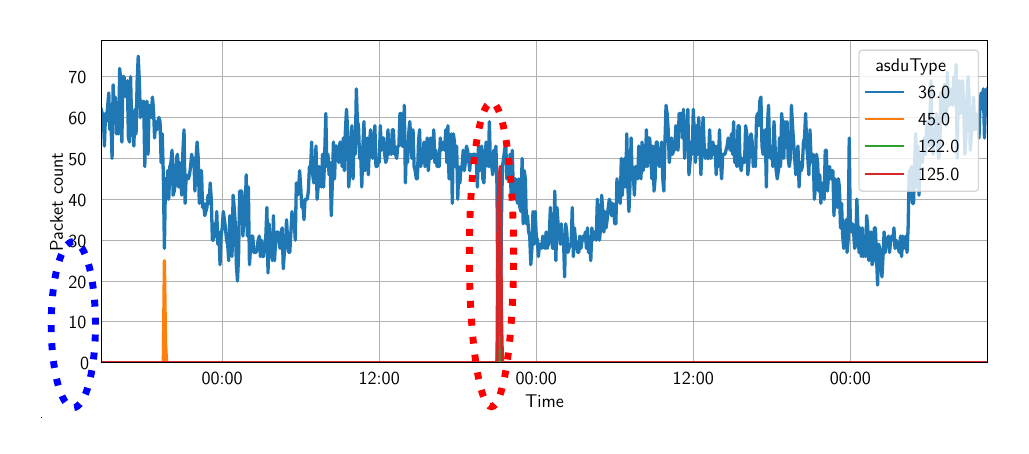
\begin{tikzpicture}
            \node(A){   
            \resizebox{1\textwidth}{!}
                {
                    %% Creator: Matplotlib, PGF backend
%%
%% To include the figure in your LaTeX document, write
%%   \input{<filename>.pgf}
%%
%% Make sure the required packages are loaded in your preamble
%%   \usepackage{pgf}
%%
%% Also ensure that all the required font packages are loaded; for instance,
%% the lmodern package is sometimes necessary when using math font.
%%   \usepackage{lmodern}
%%
%% Figures using additional raster images can only be included by \input if
%% they are in the same directory as the main LaTeX file. For loading figures
%% from other directories you can use the `import` package
%%   \usepackage{import}
%%
%% and then include the figures with
%%   \import{<path to file>}{<filename>.pgf}
%%
%% Matplotlib used the following preamble
%%   \usepackage{fontspec}
%%   \setmainfont{DejaVuSerif.ttf}[Path=\detokenize{/home/ankimme/fit/ibt/env/lib/python3.10/site-packages/matplotlib/mpl-data/fonts/ttf/}]
%%   \setsansfont{DejaVuSans.ttf}[Path=\detokenize{/home/ankimme/fit/ibt/env/lib/python3.10/site-packages/matplotlib/mpl-data/fonts/ttf/}]
%%   \setmonofont{DejaVuSansMono.ttf}[Path=\detokenize{/home/ankimme/fit/ibt/env/lib/python3.10/site-packages/matplotlib/mpl-data/fonts/ttf/}]
%%
\begingroup%
\makeatletter%
\begin{pgfpicture}%
\pgfpathrectangle{\pgfpointorigin}{\pgfqpoint{10.000000in}{4.000000in}}%
\pgfusepath{use as bounding box, clip}%
\begin{pgfscope}%
\pgfsetbuttcap%
\pgfsetmiterjoin%
\pgfsetlinewidth{0.000000pt}%
\definecolor{currentstroke}{rgb}{1.000000,1.000000,1.000000}%
\pgfsetstrokecolor{currentstroke}%
\pgfsetstrokeopacity{0.000000}%
\pgfsetdash{}{0pt}%
\pgfpathmoveto{\pgfqpoint{0.000000in}{0.000000in}}%
\pgfpathlineto{\pgfqpoint{10.000000in}{0.000000in}}%
\pgfpathlineto{\pgfqpoint{10.000000in}{4.000000in}}%
\pgfpathlineto{\pgfqpoint{0.000000in}{4.000000in}}%
\pgfpathlineto{\pgfqpoint{0.000000in}{0.000000in}}%
\pgfpathclose%
\pgfusepath{}%
\end{pgfscope}%
\begin{pgfscope}%
\pgfsetbuttcap%
\pgfsetmiterjoin%
\definecolor{currentfill}{rgb}{1.000000,1.000000,1.000000}%
\pgfsetfillcolor{currentfill}%
\pgfsetlinewidth{0.000000pt}%
\definecolor{currentstroke}{rgb}{0.000000,0.000000,0.000000}%
\pgfsetstrokecolor{currentstroke}%
\pgfsetstrokeopacity{0.000000}%
\pgfsetdash{}{0pt}%
\pgfpathmoveto{\pgfqpoint{0.630049in}{0.570804in}}%
\pgfpathlineto{\pgfqpoint{9.958330in}{0.570804in}}%
\pgfpathlineto{\pgfqpoint{9.958330in}{3.958330in}}%
\pgfpathlineto{\pgfqpoint{0.630049in}{3.958330in}}%
\pgfpathlineto{\pgfqpoint{0.630049in}{0.570804in}}%
\pgfpathclose%
\pgfusepath{fill}%
\end{pgfscope}%
\begin{pgfscope}%
\pgfpathrectangle{\pgfqpoint{0.630049in}{0.570804in}}{\pgfqpoint{9.328281in}{3.387526in}}%
\pgfusepath{clip}%
\pgfsetrectcap%
\pgfsetroundjoin%
\pgfsetlinewidth{0.803000pt}%
\definecolor{currentstroke}{rgb}{0.690196,0.690196,0.690196}%
\pgfsetstrokecolor{currentstroke}%
\pgfsetdash{}{0pt}%
\pgfpathmoveto{\pgfqpoint{1.903652in}{0.570804in}}%
\pgfpathlineto{\pgfqpoint{1.903652in}{3.958330in}}%
\pgfusepath{stroke}%
\end{pgfscope}%
\begin{pgfscope}%
\pgfsetbuttcap%
\pgfsetroundjoin%
\definecolor{currentfill}{rgb}{0.000000,0.000000,0.000000}%
\pgfsetfillcolor{currentfill}%
\pgfsetlinewidth{0.803000pt}%
\definecolor{currentstroke}{rgb}{0.000000,0.000000,0.000000}%
\pgfsetstrokecolor{currentstroke}%
\pgfsetdash{}{0pt}%
\pgfsys@defobject{currentmarker}{\pgfqpoint{0.000000in}{-0.048611in}}{\pgfqpoint{0.000000in}{0.000000in}}{%
\pgfpathmoveto{\pgfqpoint{0.000000in}{0.000000in}}%
\pgfpathlineto{\pgfqpoint{0.000000in}{-0.048611in}}%
\pgfusepath{stroke,fill}%
}%
\begin{pgfscope}%
\pgfsys@transformshift{1.903652in}{0.570804in}%
\pgfsys@useobject{currentmarker}{}%
\end{pgfscope}%
\end{pgfscope}%
\begin{pgfscope}%
\definecolor{textcolor}{rgb}{0.000000,0.000000,0.000000}%
\pgfsetstrokecolor{textcolor}%
\pgfsetfillcolor{textcolor}%
\pgftext[x=1.903652in,y=0.473582in,,top]{\color{textcolor}\sffamily\fontsize{14.000000}{16.800000}\selectfont 00:00}%
\end{pgfscope}%
\begin{pgfscope}%
\pgfpathrectangle{\pgfqpoint{0.630049in}{0.570804in}}{\pgfqpoint{9.328281in}{3.387526in}}%
\pgfusepath{clip}%
\pgfsetrectcap%
\pgfsetroundjoin%
\pgfsetlinewidth{0.803000pt}%
\definecolor{currentstroke}{rgb}{0.690196,0.690196,0.690196}%
\pgfsetstrokecolor{currentstroke}%
\pgfsetdash{}{0pt}%
\pgfpathmoveto{\pgfqpoint{3.555893in}{0.570804in}}%
\pgfpathlineto{\pgfqpoint{3.555893in}{3.958330in}}%
\pgfusepath{stroke}%
\end{pgfscope}%
\begin{pgfscope}%
\pgfsetbuttcap%
\pgfsetroundjoin%
\definecolor{currentfill}{rgb}{0.000000,0.000000,0.000000}%
\pgfsetfillcolor{currentfill}%
\pgfsetlinewidth{0.803000pt}%
\definecolor{currentstroke}{rgb}{0.000000,0.000000,0.000000}%
\pgfsetstrokecolor{currentstroke}%
\pgfsetdash{}{0pt}%
\pgfsys@defobject{currentmarker}{\pgfqpoint{0.000000in}{-0.048611in}}{\pgfqpoint{0.000000in}{0.000000in}}{%
\pgfpathmoveto{\pgfqpoint{0.000000in}{0.000000in}}%
\pgfpathlineto{\pgfqpoint{0.000000in}{-0.048611in}}%
\pgfusepath{stroke,fill}%
}%
\begin{pgfscope}%
\pgfsys@transformshift{3.555893in}{0.570804in}%
\pgfsys@useobject{currentmarker}{}%
\end{pgfscope}%
\end{pgfscope}%
\begin{pgfscope}%
\definecolor{textcolor}{rgb}{0.000000,0.000000,0.000000}%
\pgfsetstrokecolor{textcolor}%
\pgfsetfillcolor{textcolor}%
\pgftext[x=3.555893in,y=0.473582in,,top]{\color{textcolor}\sffamily\fontsize{14.000000}{16.800000}\selectfont 12:00}%
\end{pgfscope}%
\begin{pgfscope}%
\pgfpathrectangle{\pgfqpoint{0.630049in}{0.570804in}}{\pgfqpoint{9.328281in}{3.387526in}}%
\pgfusepath{clip}%
\pgfsetrectcap%
\pgfsetroundjoin%
\pgfsetlinewidth{0.803000pt}%
\definecolor{currentstroke}{rgb}{0.690196,0.690196,0.690196}%
\pgfsetstrokecolor{currentstroke}%
\pgfsetdash{}{0pt}%
\pgfpathmoveto{\pgfqpoint{5.208135in}{0.570804in}}%
\pgfpathlineto{\pgfqpoint{5.208135in}{3.958330in}}%
\pgfusepath{stroke}%
\end{pgfscope}%
\begin{pgfscope}%
\pgfsetbuttcap%
\pgfsetroundjoin%
\definecolor{currentfill}{rgb}{0.000000,0.000000,0.000000}%
\pgfsetfillcolor{currentfill}%
\pgfsetlinewidth{0.803000pt}%
\definecolor{currentstroke}{rgb}{0.000000,0.000000,0.000000}%
\pgfsetstrokecolor{currentstroke}%
\pgfsetdash{}{0pt}%
\pgfsys@defobject{currentmarker}{\pgfqpoint{0.000000in}{-0.048611in}}{\pgfqpoint{0.000000in}{0.000000in}}{%
\pgfpathmoveto{\pgfqpoint{0.000000in}{0.000000in}}%
\pgfpathlineto{\pgfqpoint{0.000000in}{-0.048611in}}%
\pgfusepath{stroke,fill}%
}%
\begin{pgfscope}%
\pgfsys@transformshift{5.208135in}{0.570804in}%
\pgfsys@useobject{currentmarker}{}%
\end{pgfscope}%
\end{pgfscope}%
\begin{pgfscope}%
\definecolor{textcolor}{rgb}{0.000000,0.000000,0.000000}%
\pgfsetstrokecolor{textcolor}%
\pgfsetfillcolor{textcolor}%
\pgftext[x=5.208135in,y=0.473582in,,top]{\color{textcolor}\sffamily\fontsize{14.000000}{16.800000}\selectfont 00:00}%
\end{pgfscope}%
\begin{pgfscope}%
\pgfpathrectangle{\pgfqpoint{0.630049in}{0.570804in}}{\pgfqpoint{9.328281in}{3.387526in}}%
\pgfusepath{clip}%
\pgfsetrectcap%
\pgfsetroundjoin%
\pgfsetlinewidth{0.803000pt}%
\definecolor{currentstroke}{rgb}{0.690196,0.690196,0.690196}%
\pgfsetstrokecolor{currentstroke}%
\pgfsetdash{}{0pt}%
\pgfpathmoveto{\pgfqpoint{6.860377in}{0.570804in}}%
\pgfpathlineto{\pgfqpoint{6.860377in}{3.958330in}}%
\pgfusepath{stroke}%
\end{pgfscope}%
\begin{pgfscope}%
\pgfsetbuttcap%
\pgfsetroundjoin%
\definecolor{currentfill}{rgb}{0.000000,0.000000,0.000000}%
\pgfsetfillcolor{currentfill}%
\pgfsetlinewidth{0.803000pt}%
\definecolor{currentstroke}{rgb}{0.000000,0.000000,0.000000}%
\pgfsetstrokecolor{currentstroke}%
\pgfsetdash{}{0pt}%
\pgfsys@defobject{currentmarker}{\pgfqpoint{0.000000in}{-0.048611in}}{\pgfqpoint{0.000000in}{0.000000in}}{%
\pgfpathmoveto{\pgfqpoint{0.000000in}{0.000000in}}%
\pgfpathlineto{\pgfqpoint{0.000000in}{-0.048611in}}%
\pgfusepath{stroke,fill}%
}%
\begin{pgfscope}%
\pgfsys@transformshift{6.860377in}{0.570804in}%
\pgfsys@useobject{currentmarker}{}%
\end{pgfscope}%
\end{pgfscope}%
\begin{pgfscope}%
\definecolor{textcolor}{rgb}{0.000000,0.000000,0.000000}%
\pgfsetstrokecolor{textcolor}%
\pgfsetfillcolor{textcolor}%
\pgftext[x=6.860377in,y=0.473582in,,top]{\color{textcolor}\sffamily\fontsize{14.000000}{16.800000}\selectfont 12:00}%
\end{pgfscope}%
\begin{pgfscope}%
\pgfpathrectangle{\pgfqpoint{0.630049in}{0.570804in}}{\pgfqpoint{9.328281in}{3.387526in}}%
\pgfusepath{clip}%
\pgfsetrectcap%
\pgfsetroundjoin%
\pgfsetlinewidth{0.803000pt}%
\definecolor{currentstroke}{rgb}{0.690196,0.690196,0.690196}%
\pgfsetstrokecolor{currentstroke}%
\pgfsetdash{}{0pt}%
\pgfpathmoveto{\pgfqpoint{8.512619in}{0.570804in}}%
\pgfpathlineto{\pgfqpoint{8.512619in}{3.958330in}}%
\pgfusepath{stroke}%
\end{pgfscope}%
\begin{pgfscope}%
\pgfsetbuttcap%
\pgfsetroundjoin%
\definecolor{currentfill}{rgb}{0.000000,0.000000,0.000000}%
\pgfsetfillcolor{currentfill}%
\pgfsetlinewidth{0.803000pt}%
\definecolor{currentstroke}{rgb}{0.000000,0.000000,0.000000}%
\pgfsetstrokecolor{currentstroke}%
\pgfsetdash{}{0pt}%
\pgfsys@defobject{currentmarker}{\pgfqpoint{0.000000in}{-0.048611in}}{\pgfqpoint{0.000000in}{0.000000in}}{%
\pgfpathmoveto{\pgfqpoint{0.000000in}{0.000000in}}%
\pgfpathlineto{\pgfqpoint{0.000000in}{-0.048611in}}%
\pgfusepath{stroke,fill}%
}%
\begin{pgfscope}%
\pgfsys@transformshift{8.512619in}{0.570804in}%
\pgfsys@useobject{currentmarker}{}%
\end{pgfscope}%
\end{pgfscope}%
\begin{pgfscope}%
\definecolor{textcolor}{rgb}{0.000000,0.000000,0.000000}%
\pgfsetstrokecolor{textcolor}%
\pgfsetfillcolor{textcolor}%
\pgftext[x=8.512619in,y=0.473582in,,top]{\color{textcolor}\sffamily\fontsize{14.000000}{16.800000}\selectfont 00:00}%
\end{pgfscope}%
\begin{pgfscope}%
\definecolor{textcolor}{rgb}{0.000000,0.000000,0.000000}%
\pgfsetstrokecolor{textcolor}%
\pgfsetfillcolor{textcolor}%
\pgftext[x=5.294189in,y=0.229848in,,top]{\color{textcolor}\sffamily\fontsize{14.000000}{16.800000}\selectfont Time}%
\end{pgfscope}%
\begin{pgfscope}%
\pgfpathrectangle{\pgfqpoint{0.630049in}{0.570804in}}{\pgfqpoint{9.328281in}{3.387526in}}%
\pgfusepath{clip}%
\pgfsetrectcap%
\pgfsetroundjoin%
\pgfsetlinewidth{0.803000pt}%
\definecolor{currentstroke}{rgb}{0.690196,0.690196,0.690196}%
\pgfsetstrokecolor{currentstroke}%
\pgfsetdash{}{0pt}%
\pgfpathmoveto{\pgfqpoint{0.630049in}{0.570804in}}%
\pgfpathlineto{\pgfqpoint{9.958330in}{0.570804in}}%
\pgfusepath{stroke}%
\end{pgfscope}%
\begin{pgfscope}%
\pgfsetbuttcap%
\pgfsetroundjoin%
\definecolor{currentfill}{rgb}{0.000000,0.000000,0.000000}%
\pgfsetfillcolor{currentfill}%
\pgfsetlinewidth{0.803000pt}%
\definecolor{currentstroke}{rgb}{0.000000,0.000000,0.000000}%
\pgfsetstrokecolor{currentstroke}%
\pgfsetdash{}{0pt}%
\pgfsys@defobject{currentmarker}{\pgfqpoint{-0.048611in}{0.000000in}}{\pgfqpoint{-0.000000in}{0.000000in}}{%
\pgfpathmoveto{\pgfqpoint{-0.000000in}{0.000000in}}%
\pgfpathlineto{\pgfqpoint{-0.048611in}{0.000000in}}%
\pgfusepath{stroke,fill}%
}%
\begin{pgfscope}%
\pgfsys@transformshift{0.630049in}{0.570804in}%
\pgfsys@useobject{currentmarker}{}%
\end{pgfscope}%
\end{pgfscope}%
\begin{pgfscope}%
\definecolor{textcolor}{rgb}{0.000000,0.000000,0.000000}%
\pgfsetstrokecolor{textcolor}%
\pgfsetfillcolor{textcolor}%
\pgftext[x=0.409115in, y=0.496938in, left, base]{\color{textcolor}\sffamily\fontsize{14.000000}{16.800000}\selectfont 0}%
\end{pgfscope}%
\begin{pgfscope}%
\pgfpathrectangle{\pgfqpoint{0.630049in}{0.570804in}}{\pgfqpoint{9.328281in}{3.387526in}}%
\pgfusepath{clip}%
\pgfsetrectcap%
\pgfsetroundjoin%
\pgfsetlinewidth{0.803000pt}%
\definecolor{currentstroke}{rgb}{0.690196,0.690196,0.690196}%
\pgfsetstrokecolor{currentstroke}%
\pgfsetdash{}{0pt}%
\pgfpathmoveto{\pgfqpoint{0.630049in}{1.000966in}}%
\pgfpathlineto{\pgfqpoint{9.958330in}{1.000966in}}%
\pgfusepath{stroke}%
\end{pgfscope}%
\begin{pgfscope}%
\pgfsetbuttcap%
\pgfsetroundjoin%
\definecolor{currentfill}{rgb}{0.000000,0.000000,0.000000}%
\pgfsetfillcolor{currentfill}%
\pgfsetlinewidth{0.803000pt}%
\definecolor{currentstroke}{rgb}{0.000000,0.000000,0.000000}%
\pgfsetstrokecolor{currentstroke}%
\pgfsetdash{}{0pt}%
\pgfsys@defobject{currentmarker}{\pgfqpoint{-0.048611in}{0.000000in}}{\pgfqpoint{-0.000000in}{0.000000in}}{%
\pgfpathmoveto{\pgfqpoint{-0.000000in}{0.000000in}}%
\pgfpathlineto{\pgfqpoint{-0.048611in}{0.000000in}}%
\pgfusepath{stroke,fill}%
}%
\begin{pgfscope}%
\pgfsys@transformshift{0.630049in}{1.000966in}%
\pgfsys@useobject{currentmarker}{}%
\end{pgfscope}%
\end{pgfscope}%
\begin{pgfscope}%
\definecolor{textcolor}{rgb}{0.000000,0.000000,0.000000}%
\pgfsetstrokecolor{textcolor}%
\pgfsetfillcolor{textcolor}%
\pgftext[x=0.285404in, y=0.927100in, left, base]{\color{textcolor}\sffamily\fontsize{14.000000}{16.800000}\selectfont 10}%
\end{pgfscope}%
\begin{pgfscope}%
\pgfpathrectangle{\pgfqpoint{0.630049in}{0.570804in}}{\pgfqpoint{9.328281in}{3.387526in}}%
\pgfusepath{clip}%
\pgfsetrectcap%
\pgfsetroundjoin%
\pgfsetlinewidth{0.803000pt}%
\definecolor{currentstroke}{rgb}{0.690196,0.690196,0.690196}%
\pgfsetstrokecolor{currentstroke}%
\pgfsetdash{}{0pt}%
\pgfpathmoveto{\pgfqpoint{0.630049in}{1.431128in}}%
\pgfpathlineto{\pgfqpoint{9.958330in}{1.431128in}}%
\pgfusepath{stroke}%
\end{pgfscope}%
\begin{pgfscope}%
\pgfsetbuttcap%
\pgfsetroundjoin%
\definecolor{currentfill}{rgb}{0.000000,0.000000,0.000000}%
\pgfsetfillcolor{currentfill}%
\pgfsetlinewidth{0.803000pt}%
\definecolor{currentstroke}{rgb}{0.000000,0.000000,0.000000}%
\pgfsetstrokecolor{currentstroke}%
\pgfsetdash{}{0pt}%
\pgfsys@defobject{currentmarker}{\pgfqpoint{-0.048611in}{0.000000in}}{\pgfqpoint{-0.000000in}{0.000000in}}{%
\pgfpathmoveto{\pgfqpoint{-0.000000in}{0.000000in}}%
\pgfpathlineto{\pgfqpoint{-0.048611in}{0.000000in}}%
\pgfusepath{stroke,fill}%
}%
\begin{pgfscope}%
\pgfsys@transformshift{0.630049in}{1.431128in}%
\pgfsys@useobject{currentmarker}{}%
\end{pgfscope}%
\end{pgfscope}%
\begin{pgfscope}%
\definecolor{textcolor}{rgb}{0.000000,0.000000,0.000000}%
\pgfsetstrokecolor{textcolor}%
\pgfsetfillcolor{textcolor}%
\pgftext[x=0.285404in, y=1.357262in, left, base]{\color{textcolor}\sffamily\fontsize{14.000000}{16.800000}\selectfont 20}%
\end{pgfscope}%
\begin{pgfscope}%
\pgfpathrectangle{\pgfqpoint{0.630049in}{0.570804in}}{\pgfqpoint{9.328281in}{3.387526in}}%
\pgfusepath{clip}%
\pgfsetrectcap%
\pgfsetroundjoin%
\pgfsetlinewidth{0.803000pt}%
\definecolor{currentstroke}{rgb}{0.690196,0.690196,0.690196}%
\pgfsetstrokecolor{currentstroke}%
\pgfsetdash{}{0pt}%
\pgfpathmoveto{\pgfqpoint{0.630049in}{1.861290in}}%
\pgfpathlineto{\pgfqpoint{9.958330in}{1.861290in}}%
\pgfusepath{stroke}%
\end{pgfscope}%
\begin{pgfscope}%
\pgfsetbuttcap%
\pgfsetroundjoin%
\definecolor{currentfill}{rgb}{0.000000,0.000000,0.000000}%
\pgfsetfillcolor{currentfill}%
\pgfsetlinewidth{0.803000pt}%
\definecolor{currentstroke}{rgb}{0.000000,0.000000,0.000000}%
\pgfsetstrokecolor{currentstroke}%
\pgfsetdash{}{0pt}%
\pgfsys@defobject{currentmarker}{\pgfqpoint{-0.048611in}{0.000000in}}{\pgfqpoint{-0.000000in}{0.000000in}}{%
\pgfpathmoveto{\pgfqpoint{-0.000000in}{0.000000in}}%
\pgfpathlineto{\pgfqpoint{-0.048611in}{0.000000in}}%
\pgfusepath{stroke,fill}%
}%
\begin{pgfscope}%
\pgfsys@transformshift{0.630049in}{1.861290in}%
\pgfsys@useobject{currentmarker}{}%
\end{pgfscope}%
\end{pgfscope}%
\begin{pgfscope}%
\definecolor{textcolor}{rgb}{0.000000,0.000000,0.000000}%
\pgfsetstrokecolor{textcolor}%
\pgfsetfillcolor{textcolor}%
\pgftext[x=0.285404in, y=1.787424in, left, base]{\color{textcolor}\sffamily\fontsize{14.000000}{16.800000}\selectfont 30}%
\end{pgfscope}%
\begin{pgfscope}%
\pgfpathrectangle{\pgfqpoint{0.630049in}{0.570804in}}{\pgfqpoint{9.328281in}{3.387526in}}%
\pgfusepath{clip}%
\pgfsetrectcap%
\pgfsetroundjoin%
\pgfsetlinewidth{0.803000pt}%
\definecolor{currentstroke}{rgb}{0.690196,0.690196,0.690196}%
\pgfsetstrokecolor{currentstroke}%
\pgfsetdash{}{0pt}%
\pgfpathmoveto{\pgfqpoint{0.630049in}{2.291452in}}%
\pgfpathlineto{\pgfqpoint{9.958330in}{2.291452in}}%
\pgfusepath{stroke}%
\end{pgfscope}%
\begin{pgfscope}%
\pgfsetbuttcap%
\pgfsetroundjoin%
\definecolor{currentfill}{rgb}{0.000000,0.000000,0.000000}%
\pgfsetfillcolor{currentfill}%
\pgfsetlinewidth{0.803000pt}%
\definecolor{currentstroke}{rgb}{0.000000,0.000000,0.000000}%
\pgfsetstrokecolor{currentstroke}%
\pgfsetdash{}{0pt}%
\pgfsys@defobject{currentmarker}{\pgfqpoint{-0.048611in}{0.000000in}}{\pgfqpoint{-0.000000in}{0.000000in}}{%
\pgfpathmoveto{\pgfqpoint{-0.000000in}{0.000000in}}%
\pgfpathlineto{\pgfqpoint{-0.048611in}{0.000000in}}%
\pgfusepath{stroke,fill}%
}%
\begin{pgfscope}%
\pgfsys@transformshift{0.630049in}{2.291452in}%
\pgfsys@useobject{currentmarker}{}%
\end{pgfscope}%
\end{pgfscope}%
\begin{pgfscope}%
\definecolor{textcolor}{rgb}{0.000000,0.000000,0.000000}%
\pgfsetstrokecolor{textcolor}%
\pgfsetfillcolor{textcolor}%
\pgftext[x=0.285404in, y=2.217586in, left, base]{\color{textcolor}\sffamily\fontsize{14.000000}{16.800000}\selectfont 40}%
\end{pgfscope}%
\begin{pgfscope}%
\pgfpathrectangle{\pgfqpoint{0.630049in}{0.570804in}}{\pgfqpoint{9.328281in}{3.387526in}}%
\pgfusepath{clip}%
\pgfsetrectcap%
\pgfsetroundjoin%
\pgfsetlinewidth{0.803000pt}%
\definecolor{currentstroke}{rgb}{0.690196,0.690196,0.690196}%
\pgfsetstrokecolor{currentstroke}%
\pgfsetdash{}{0pt}%
\pgfpathmoveto{\pgfqpoint{0.630049in}{2.721614in}}%
\pgfpathlineto{\pgfqpoint{9.958330in}{2.721614in}}%
\pgfusepath{stroke}%
\end{pgfscope}%
\begin{pgfscope}%
\pgfsetbuttcap%
\pgfsetroundjoin%
\definecolor{currentfill}{rgb}{0.000000,0.000000,0.000000}%
\pgfsetfillcolor{currentfill}%
\pgfsetlinewidth{0.803000pt}%
\definecolor{currentstroke}{rgb}{0.000000,0.000000,0.000000}%
\pgfsetstrokecolor{currentstroke}%
\pgfsetdash{}{0pt}%
\pgfsys@defobject{currentmarker}{\pgfqpoint{-0.048611in}{0.000000in}}{\pgfqpoint{-0.000000in}{0.000000in}}{%
\pgfpathmoveto{\pgfqpoint{-0.000000in}{0.000000in}}%
\pgfpathlineto{\pgfqpoint{-0.048611in}{0.000000in}}%
\pgfusepath{stroke,fill}%
}%
\begin{pgfscope}%
\pgfsys@transformshift{0.630049in}{2.721614in}%
\pgfsys@useobject{currentmarker}{}%
\end{pgfscope}%
\end{pgfscope}%
\begin{pgfscope}%
\definecolor{textcolor}{rgb}{0.000000,0.000000,0.000000}%
\pgfsetstrokecolor{textcolor}%
\pgfsetfillcolor{textcolor}%
\pgftext[x=0.285404in, y=2.647748in, left, base]{\color{textcolor}\sffamily\fontsize{14.000000}{16.800000}\selectfont 50}%
\end{pgfscope}%
\begin{pgfscope}%
\pgfpathrectangle{\pgfqpoint{0.630049in}{0.570804in}}{\pgfqpoint{9.328281in}{3.387526in}}%
\pgfusepath{clip}%
\pgfsetrectcap%
\pgfsetroundjoin%
\pgfsetlinewidth{0.803000pt}%
\definecolor{currentstroke}{rgb}{0.690196,0.690196,0.690196}%
\pgfsetstrokecolor{currentstroke}%
\pgfsetdash{}{0pt}%
\pgfpathmoveto{\pgfqpoint{0.630049in}{3.151776in}}%
\pgfpathlineto{\pgfqpoint{9.958330in}{3.151776in}}%
\pgfusepath{stroke}%
\end{pgfscope}%
\begin{pgfscope}%
\pgfsetbuttcap%
\pgfsetroundjoin%
\definecolor{currentfill}{rgb}{0.000000,0.000000,0.000000}%
\pgfsetfillcolor{currentfill}%
\pgfsetlinewidth{0.803000pt}%
\definecolor{currentstroke}{rgb}{0.000000,0.000000,0.000000}%
\pgfsetstrokecolor{currentstroke}%
\pgfsetdash{}{0pt}%
\pgfsys@defobject{currentmarker}{\pgfqpoint{-0.048611in}{0.000000in}}{\pgfqpoint{-0.000000in}{0.000000in}}{%
\pgfpathmoveto{\pgfqpoint{-0.000000in}{0.000000in}}%
\pgfpathlineto{\pgfqpoint{-0.048611in}{0.000000in}}%
\pgfusepath{stroke,fill}%
}%
\begin{pgfscope}%
\pgfsys@transformshift{0.630049in}{3.151776in}%
\pgfsys@useobject{currentmarker}{}%
\end{pgfscope}%
\end{pgfscope}%
\begin{pgfscope}%
\definecolor{textcolor}{rgb}{0.000000,0.000000,0.000000}%
\pgfsetstrokecolor{textcolor}%
\pgfsetfillcolor{textcolor}%
\pgftext[x=0.285404in, y=3.077910in, left, base]{\color{textcolor}\sffamily\fontsize{14.000000}{16.800000}\selectfont 60}%
\end{pgfscope}%
\begin{pgfscope}%
\pgfpathrectangle{\pgfqpoint{0.630049in}{0.570804in}}{\pgfqpoint{9.328281in}{3.387526in}}%
\pgfusepath{clip}%
\pgfsetrectcap%
\pgfsetroundjoin%
\pgfsetlinewidth{0.803000pt}%
\definecolor{currentstroke}{rgb}{0.690196,0.690196,0.690196}%
\pgfsetstrokecolor{currentstroke}%
\pgfsetdash{}{0pt}%
\pgfpathmoveto{\pgfqpoint{0.630049in}{3.581938in}}%
\pgfpathlineto{\pgfqpoint{9.958330in}{3.581938in}}%
\pgfusepath{stroke}%
\end{pgfscope}%
\begin{pgfscope}%
\pgfsetbuttcap%
\pgfsetroundjoin%
\definecolor{currentfill}{rgb}{0.000000,0.000000,0.000000}%
\pgfsetfillcolor{currentfill}%
\pgfsetlinewidth{0.803000pt}%
\definecolor{currentstroke}{rgb}{0.000000,0.000000,0.000000}%
\pgfsetstrokecolor{currentstroke}%
\pgfsetdash{}{0pt}%
\pgfsys@defobject{currentmarker}{\pgfqpoint{-0.048611in}{0.000000in}}{\pgfqpoint{-0.000000in}{0.000000in}}{%
\pgfpathmoveto{\pgfqpoint{-0.000000in}{0.000000in}}%
\pgfpathlineto{\pgfqpoint{-0.048611in}{0.000000in}}%
\pgfusepath{stroke,fill}%
}%
\begin{pgfscope}%
\pgfsys@transformshift{0.630049in}{3.581938in}%
\pgfsys@useobject{currentmarker}{}%
\end{pgfscope}%
\end{pgfscope}%
\begin{pgfscope}%
\definecolor{textcolor}{rgb}{0.000000,0.000000,0.000000}%
\pgfsetstrokecolor{textcolor}%
\pgfsetfillcolor{textcolor}%
\pgftext[x=0.285404in, y=3.508072in, left, base]{\color{textcolor}\sffamily\fontsize{14.000000}{16.800000}\selectfont 70}%
\end{pgfscope}%
\begin{pgfscope}%
\definecolor{textcolor}{rgb}{0.000000,0.000000,0.000000}%
\pgfsetstrokecolor{textcolor}%
\pgfsetfillcolor{textcolor}%
\pgftext[x=0.229848in,y=2.264567in,,bottom,rotate=90.000000]{\color{textcolor}\sffamily\fontsize{14.000000}{16.800000}\selectfont Packet count}%
\end{pgfscope}%
\begin{pgfscope}%
\pgfpathrectangle{\pgfqpoint{0.630049in}{0.570804in}}{\pgfqpoint{9.328281in}{3.387526in}}%
\pgfusepath{clip}%
\pgfsetrectcap%
\pgfsetroundjoin%
\pgfsetlinewidth{2.509375pt}%
\definecolor{currentstroke}{rgb}{0.121569,0.466667,0.705882}%
\pgfsetstrokecolor{currentstroke}%
\pgfsetdash{}{0pt}%
\pgfpathmoveto{\pgfqpoint{0.630049in}{3.237809in}}%
\pgfpathlineto{\pgfqpoint{0.652997in}{3.151776in}}%
\pgfpathlineto{\pgfqpoint{0.664470in}{2.850663in}}%
\pgfpathlineto{\pgfqpoint{0.675944in}{3.194792in}}%
\pgfpathlineto{\pgfqpoint{0.687418in}{3.108760in}}%
\pgfpathlineto{\pgfqpoint{0.698892in}{3.280825in}}%
\pgfpathlineto{\pgfqpoint{0.710366in}{3.409873in}}%
\pgfpathlineto{\pgfqpoint{0.721840in}{3.022728in}}%
\pgfpathlineto{\pgfqpoint{0.733314in}{3.108760in}}%
\pgfpathlineto{\pgfqpoint{0.744788in}{2.721614in}}%
\pgfpathlineto{\pgfqpoint{0.756262in}{3.495906in}}%
\pgfpathlineto{\pgfqpoint{0.767736in}{3.108760in}}%
\pgfpathlineto{\pgfqpoint{0.779209in}{3.366857in}}%
\pgfpathlineto{\pgfqpoint{0.790683in}{2.979711in}}%
\pgfpathlineto{\pgfqpoint{0.802157in}{3.022728in}}%
\pgfpathlineto{\pgfqpoint{0.813631in}{2.979711in}}%
\pgfpathlineto{\pgfqpoint{0.825105in}{3.667971in}}%
\pgfpathlineto{\pgfqpoint{0.836579in}{3.538922in}}%
\pgfpathlineto{\pgfqpoint{0.848053in}{2.893679in}}%
\pgfpathlineto{\pgfqpoint{0.859527in}{3.581938in}}%
\pgfpathlineto{\pgfqpoint{0.871001in}{3.581938in}}%
\pgfpathlineto{\pgfqpoint{0.882475in}{3.409873in}}%
\pgfpathlineto{\pgfqpoint{0.893948in}{3.366857in}}%
\pgfpathlineto{\pgfqpoint{0.905422in}{3.538922in}}%
\pgfpathlineto{\pgfqpoint{0.916896in}{2.936695in}}%
\pgfpathlineto{\pgfqpoint{0.928370in}{2.893679in}}%
\pgfpathlineto{\pgfqpoint{0.939844in}{3.581938in}}%
\pgfpathlineto{\pgfqpoint{0.951318in}{3.065744in}}%
\pgfpathlineto{\pgfqpoint{0.962792in}{3.065744in}}%
\pgfpathlineto{\pgfqpoint{0.974266in}{2.850663in}}%
\pgfpathlineto{\pgfqpoint{0.985740in}{3.237809in}}%
\pgfpathlineto{\pgfqpoint{0.997214in}{2.979711in}}%
\pgfpathlineto{\pgfqpoint{1.008687in}{3.538922in}}%
\pgfpathlineto{\pgfqpoint{1.020161in}{3.797019in}}%
\pgfpathlineto{\pgfqpoint{1.031635in}{3.538922in}}%
\pgfpathlineto{\pgfqpoint{1.043109in}{3.151776in}}%
\pgfpathlineto{\pgfqpoint{1.054583in}{3.323841in}}%
\pgfpathlineto{\pgfqpoint{1.066057in}{3.280825in}}%
\pgfpathlineto{\pgfqpoint{1.077531in}{3.323841in}}%
\pgfpathlineto{\pgfqpoint{1.089005in}{2.635582in}}%
\pgfpathlineto{\pgfqpoint{1.100479in}{3.108760in}}%
\pgfpathlineto{\pgfqpoint{1.111953in}{3.323841in}}%
\pgfpathlineto{\pgfqpoint{1.123426in}{2.764630in}}%
\pgfpathlineto{\pgfqpoint{1.134900in}{3.280825in}}%
\pgfpathlineto{\pgfqpoint{1.146374in}{3.237809in}}%
\pgfpathlineto{\pgfqpoint{1.157848in}{3.151776in}}%
\pgfpathlineto{\pgfqpoint{1.169322in}{3.366857in}}%
\pgfpathlineto{\pgfqpoint{1.180796in}{3.237809in}}%
\pgfpathlineto{\pgfqpoint{1.192270in}{2.936695in}}%
\pgfpathlineto{\pgfqpoint{1.203744in}{3.108760in}}%
\pgfpathlineto{\pgfqpoint{1.215218in}{3.022728in}}%
\pgfpathlineto{\pgfqpoint{1.226692in}{3.108760in}}%
\pgfpathlineto{\pgfqpoint{1.238165in}{3.151776in}}%
\pgfpathlineto{\pgfqpoint{1.249639in}{3.108760in}}%
\pgfpathlineto{\pgfqpoint{1.261113in}{2.678598in}}%
\pgfpathlineto{\pgfqpoint{1.272587in}{2.979711in}}%
\pgfpathlineto{\pgfqpoint{1.284061in}{2.549549in}}%
\pgfpathlineto{\pgfqpoint{1.295535in}{1.775258in}}%
\pgfpathlineto{\pgfqpoint{1.307009in}{2.506533in}}%
\pgfpathlineto{\pgfqpoint{1.318483in}{2.291452in}}%
\pgfpathlineto{\pgfqpoint{1.329957in}{2.592566in}}%
\pgfpathlineto{\pgfqpoint{1.341431in}{2.291452in}}%
\pgfpathlineto{\pgfqpoint{1.352904in}{2.635582in}}%
\pgfpathlineto{\pgfqpoint{1.364378in}{2.678598in}}%
\pgfpathlineto{\pgfqpoint{1.375852in}{2.807647in}}%
\pgfpathlineto{\pgfqpoint{1.387326in}{2.334468in}}%
\pgfpathlineto{\pgfqpoint{1.398800in}{2.377484in}}%
\pgfpathlineto{\pgfqpoint{1.410274in}{2.463517in}}%
\pgfpathlineto{\pgfqpoint{1.421748in}{2.721614in}}%
\pgfpathlineto{\pgfqpoint{1.433222in}{2.764630in}}%
\pgfpathlineto{\pgfqpoint{1.444696in}{2.420501in}}%
\pgfpathlineto{\pgfqpoint{1.456170in}{2.678598in}}%
\pgfpathlineto{\pgfqpoint{1.467643in}{2.463517in}}%
\pgfpathlineto{\pgfqpoint{1.479117in}{2.334468in}}%
\pgfpathlineto{\pgfqpoint{1.490591in}{2.807647in}}%
\pgfpathlineto{\pgfqpoint{1.502065in}{3.022728in}}%
\pgfpathlineto{\pgfqpoint{1.513539in}{2.248436in}}%
\pgfpathlineto{\pgfqpoint{1.525013in}{2.549549in}}%
\pgfpathlineto{\pgfqpoint{1.536487in}{2.506533in}}%
\pgfpathlineto{\pgfqpoint{1.547961in}{2.506533in}}%
\pgfpathlineto{\pgfqpoint{1.559435in}{2.549549in}}%
\pgfpathlineto{\pgfqpoint{1.570909in}{2.635582in}}%
\pgfpathlineto{\pgfqpoint{1.582383in}{2.764630in}}%
\pgfpathlineto{\pgfqpoint{1.593856in}{2.678598in}}%
\pgfpathlineto{\pgfqpoint{1.605330in}{2.721614in}}%
\pgfpathlineto{\pgfqpoint{1.616804in}{2.377484in}}%
\pgfpathlineto{\pgfqpoint{1.628278in}{2.721614in}}%
\pgfpathlineto{\pgfqpoint{1.639752in}{2.893679in}}%
\pgfpathlineto{\pgfqpoint{1.651226in}{2.721614in}}%
\pgfpathlineto{\pgfqpoint{1.662700in}{2.248436in}}%
\pgfpathlineto{\pgfqpoint{1.674174in}{2.592566in}}%
\pgfpathlineto{\pgfqpoint{1.685648in}{2.592566in}}%
\pgfpathlineto{\pgfqpoint{1.697122in}{2.205420in}}%
\pgfpathlineto{\pgfqpoint{1.708595in}{2.248436in}}%
\pgfpathlineto{\pgfqpoint{1.720069in}{2.119387in}}%
\pgfpathlineto{\pgfqpoint{1.743017in}{2.205420in}}%
\pgfpathlineto{\pgfqpoint{1.754491in}{2.334468in}}%
\pgfpathlineto{\pgfqpoint{1.765965in}{2.248436in}}%
\pgfpathlineto{\pgfqpoint{1.777439in}{2.463517in}}%
\pgfpathlineto{\pgfqpoint{1.788913in}{2.291452in}}%
\pgfpathlineto{\pgfqpoint{1.800387in}{1.861290in}}%
\pgfpathlineto{\pgfqpoint{1.811861in}{1.861290in}}%
\pgfpathlineto{\pgfqpoint{1.823334in}{2.033355in}}%
\pgfpathlineto{\pgfqpoint{1.834808in}{1.904306in}}%
\pgfpathlineto{\pgfqpoint{1.846282in}{2.162403in}}%
\pgfpathlineto{\pgfqpoint{1.857756in}{1.818274in}}%
\pgfpathlineto{\pgfqpoint{1.869230in}{1.947322in}}%
\pgfpathlineto{\pgfqpoint{1.880704in}{1.603193in}}%
\pgfpathlineto{\pgfqpoint{1.892178in}{1.904306in}}%
\pgfpathlineto{\pgfqpoint{1.903652in}{1.990339in}}%
\pgfpathlineto{\pgfqpoint{1.915126in}{2.162403in}}%
\pgfpathlineto{\pgfqpoint{1.938073in}{1.990339in}}%
\pgfpathlineto{\pgfqpoint{1.949547in}{1.861290in}}%
\pgfpathlineto{\pgfqpoint{1.961021in}{1.818274in}}%
\pgfpathlineto{\pgfqpoint{1.972495in}{1.646209in}}%
\pgfpathlineto{\pgfqpoint{1.983969in}{2.119387in}}%
\pgfpathlineto{\pgfqpoint{1.995443in}{1.818274in}}%
\pgfpathlineto{\pgfqpoint{2.006917in}{1.689225in}}%
\pgfpathlineto{\pgfqpoint{2.018391in}{2.334468in}}%
\pgfpathlineto{\pgfqpoint{2.029865in}{2.205420in}}%
\pgfpathlineto{\pgfqpoint{2.041339in}{2.033355in}}%
\pgfpathlineto{\pgfqpoint{2.052812in}{1.603193in}}%
\pgfpathlineto{\pgfqpoint{2.064286in}{1.431128in}}%
\pgfpathlineto{\pgfqpoint{2.075760in}{1.689225in}}%
\pgfpathlineto{\pgfqpoint{2.087234in}{2.377484in}}%
\pgfpathlineto{\pgfqpoint{2.110182in}{2.377484in}}%
\pgfpathlineto{\pgfqpoint{2.121656in}{1.904306in}}%
\pgfpathlineto{\pgfqpoint{2.133130in}{2.162403in}}%
\pgfpathlineto{\pgfqpoint{2.144604in}{2.119387in}}%
\pgfpathlineto{\pgfqpoint{2.156078in}{2.549549in}}%
\pgfpathlineto{\pgfqpoint{2.167551in}{1.904306in}}%
\pgfpathlineto{\pgfqpoint{2.179025in}{2.420501in}}%
\pgfpathlineto{\pgfqpoint{2.190499in}{1.603193in}}%
\pgfpathlineto{\pgfqpoint{2.201973in}{1.775258in}}%
\pgfpathlineto{\pgfqpoint{2.213447in}{1.904306in}}%
\pgfpathlineto{\pgfqpoint{2.224921in}{1.904306in}}%
\pgfpathlineto{\pgfqpoint{2.236395in}{1.732241in}}%
\pgfpathlineto{\pgfqpoint{2.259343in}{1.732241in}}%
\pgfpathlineto{\pgfqpoint{2.270817in}{1.775258in}}%
\pgfpathlineto{\pgfqpoint{2.282290in}{1.861290in}}%
\pgfpathlineto{\pgfqpoint{2.293764in}{1.904306in}}%
\pgfpathlineto{\pgfqpoint{2.305238in}{1.689225in}}%
\pgfpathlineto{\pgfqpoint{2.316712in}{1.861290in}}%
\pgfpathlineto{\pgfqpoint{2.328186in}{1.689225in}}%
\pgfpathlineto{\pgfqpoint{2.339660in}{1.689225in}}%
\pgfpathlineto{\pgfqpoint{2.351134in}{1.775258in}}%
\pgfpathlineto{\pgfqpoint{2.362608in}{1.904306in}}%
\pgfpathlineto{\pgfqpoint{2.374082in}{2.205420in}}%
\pgfpathlineto{\pgfqpoint{2.385556in}{1.517160in}}%
\pgfpathlineto{\pgfqpoint{2.397029in}{2.033355in}}%
\pgfpathlineto{\pgfqpoint{2.408503in}{1.689225in}}%
\pgfpathlineto{\pgfqpoint{2.419977in}{1.732241in}}%
\pgfpathlineto{\pgfqpoint{2.431451in}{1.646209in}}%
\pgfpathlineto{\pgfqpoint{2.442925in}{2.119387in}}%
\pgfpathlineto{\pgfqpoint{2.454399in}{1.646209in}}%
\pgfpathlineto{\pgfqpoint{2.465873in}{1.861290in}}%
\pgfpathlineto{\pgfqpoint{2.477347in}{1.947322in}}%
\pgfpathlineto{\pgfqpoint{2.488821in}{1.947322in}}%
\pgfpathlineto{\pgfqpoint{2.511768in}{1.775258in}}%
\pgfpathlineto{\pgfqpoint{2.523242in}{1.947322in}}%
\pgfpathlineto{\pgfqpoint{2.534716in}{1.990339in}}%
\pgfpathlineto{\pgfqpoint{2.546190in}{1.560177in}}%
\pgfpathlineto{\pgfqpoint{2.557664in}{1.732241in}}%
\pgfpathlineto{\pgfqpoint{2.569138in}{1.818274in}}%
\pgfpathlineto{\pgfqpoint{2.580612in}{2.076371in}}%
\pgfpathlineto{\pgfqpoint{2.592086in}{1.861290in}}%
\pgfpathlineto{\pgfqpoint{2.603560in}{1.732241in}}%
\pgfpathlineto{\pgfqpoint{2.615034in}{1.732241in}}%
\pgfpathlineto{\pgfqpoint{2.637981in}{2.162403in}}%
\pgfpathlineto{\pgfqpoint{2.649455in}{1.990339in}}%
\pgfpathlineto{\pgfqpoint{2.660929in}{2.076371in}}%
\pgfpathlineto{\pgfqpoint{2.672403in}{1.861290in}}%
\pgfpathlineto{\pgfqpoint{2.683877in}{2.463517in}}%
\pgfpathlineto{\pgfqpoint{2.695351in}{2.334468in}}%
\pgfpathlineto{\pgfqpoint{2.706825in}{2.377484in}}%
\pgfpathlineto{\pgfqpoint{2.718299in}{2.592566in}}%
\pgfpathlineto{\pgfqpoint{2.729773in}{2.420501in}}%
\pgfpathlineto{\pgfqpoint{2.741246in}{2.205420in}}%
\pgfpathlineto{\pgfqpoint{2.752720in}{2.248436in}}%
\pgfpathlineto{\pgfqpoint{2.764194in}{2.076371in}}%
\pgfpathlineto{\pgfqpoint{2.775668in}{2.291452in}}%
\pgfpathlineto{\pgfqpoint{2.798616in}{2.291452in}}%
\pgfpathlineto{\pgfqpoint{2.810090in}{2.377484in}}%
\pgfpathlineto{\pgfqpoint{2.821564in}{2.635582in}}%
\pgfpathlineto{\pgfqpoint{2.833038in}{2.592566in}}%
\pgfpathlineto{\pgfqpoint{2.844512in}{2.893679in}}%
\pgfpathlineto{\pgfqpoint{2.855985in}{2.549549in}}%
\pgfpathlineto{\pgfqpoint{2.867459in}{2.463517in}}%
\pgfpathlineto{\pgfqpoint{2.878933in}{2.506533in}}%
\pgfpathlineto{\pgfqpoint{2.890407in}{2.850663in}}%
\pgfpathlineto{\pgfqpoint{2.901881in}{2.291452in}}%
\pgfpathlineto{\pgfqpoint{2.913355in}{2.420501in}}%
\pgfpathlineto{\pgfqpoint{2.924829in}{2.635582in}}%
\pgfpathlineto{\pgfqpoint{2.936303in}{2.549549in}}%
\pgfpathlineto{\pgfqpoint{2.947777in}{2.420501in}}%
\pgfpathlineto{\pgfqpoint{2.959251in}{2.764630in}}%
\pgfpathlineto{\pgfqpoint{2.970724in}{2.420501in}}%
\pgfpathlineto{\pgfqpoint{2.982198in}{2.764630in}}%
\pgfpathlineto{\pgfqpoint{2.993672in}{3.194792in}}%
\pgfpathlineto{\pgfqpoint{3.005146in}{2.635582in}}%
\pgfpathlineto{\pgfqpoint{3.016620in}{2.764630in}}%
\pgfpathlineto{\pgfqpoint{3.028094in}{2.549549in}}%
\pgfpathlineto{\pgfqpoint{3.039568in}{2.678598in}}%
\pgfpathlineto{\pgfqpoint{3.051042in}{2.119387in}}%
\pgfpathlineto{\pgfqpoint{3.062516in}{2.463517in}}%
\pgfpathlineto{\pgfqpoint{3.073990in}{2.893679in}}%
\pgfpathlineto{\pgfqpoint{3.085463in}{2.506533in}}%
\pgfpathlineto{\pgfqpoint{3.096937in}{2.850663in}}%
\pgfpathlineto{\pgfqpoint{3.108411in}{2.850663in}}%
\pgfpathlineto{\pgfqpoint{3.131359in}{2.678598in}}%
\pgfpathlineto{\pgfqpoint{3.142833in}{2.893679in}}%
\pgfpathlineto{\pgfqpoint{3.154307in}{2.807647in}}%
\pgfpathlineto{\pgfqpoint{3.165781in}{2.635582in}}%
\pgfpathlineto{\pgfqpoint{3.177255in}{2.936695in}}%
\pgfpathlineto{\pgfqpoint{3.188729in}{2.592566in}}%
\pgfpathlineto{\pgfqpoint{3.200203in}{3.022728in}}%
\pgfpathlineto{\pgfqpoint{3.211676in}{3.237809in}}%
\pgfpathlineto{\pgfqpoint{3.223150in}{3.022728in}}%
\pgfpathlineto{\pgfqpoint{3.234624in}{2.420501in}}%
\pgfpathlineto{\pgfqpoint{3.246098in}{2.592566in}}%
\pgfpathlineto{\pgfqpoint{3.257572in}{2.850663in}}%
\pgfpathlineto{\pgfqpoint{3.269046in}{3.065744in}}%
\pgfpathlineto{\pgfqpoint{3.280520in}{2.506533in}}%
\pgfpathlineto{\pgfqpoint{3.291994in}{2.979711in}}%
\pgfpathlineto{\pgfqpoint{3.303468in}{2.764630in}}%
\pgfpathlineto{\pgfqpoint{3.314942in}{3.452890in}}%
\pgfpathlineto{\pgfqpoint{3.326415in}{3.108760in}}%
\pgfpathlineto{\pgfqpoint{3.337889in}{3.065744in}}%
\pgfpathlineto{\pgfqpoint{3.349363in}{2.721614in}}%
\pgfpathlineto{\pgfqpoint{3.360837in}{2.764630in}}%
\pgfpathlineto{\pgfqpoint{3.372311in}{2.420501in}}%
\pgfpathlineto{\pgfqpoint{3.383785in}{2.850663in}}%
\pgfpathlineto{\pgfqpoint{3.395259in}{3.108760in}}%
\pgfpathlineto{\pgfqpoint{3.406733in}{2.592566in}}%
\pgfpathlineto{\pgfqpoint{3.418207in}{2.807647in}}%
\pgfpathlineto{\pgfqpoint{3.429681in}{2.936695in}}%
\pgfpathlineto{\pgfqpoint{3.441154in}{2.549549in}}%
\pgfpathlineto{\pgfqpoint{3.452628in}{2.850663in}}%
\pgfpathlineto{\pgfqpoint{3.464102in}{3.022728in}}%
\pgfpathlineto{\pgfqpoint{3.475576in}{2.893679in}}%
\pgfpathlineto{\pgfqpoint{3.487050in}{2.721614in}}%
\pgfpathlineto{\pgfqpoint{3.509998in}{3.065744in}}%
\pgfpathlineto{\pgfqpoint{3.521472in}{2.635582in}}%
\pgfpathlineto{\pgfqpoint{3.532946in}{2.635582in}}%
\pgfpathlineto{\pgfqpoint{3.544420in}{2.678598in}}%
\pgfpathlineto{\pgfqpoint{3.555893in}{2.678598in}}%
\pgfpathlineto{\pgfqpoint{3.567367in}{3.065744in}}%
\pgfpathlineto{\pgfqpoint{3.578841in}{2.807647in}}%
\pgfpathlineto{\pgfqpoint{3.590315in}{2.936695in}}%
\pgfpathlineto{\pgfqpoint{3.601789in}{2.936695in}}%
\pgfpathlineto{\pgfqpoint{3.613263in}{2.764630in}}%
\pgfpathlineto{\pgfqpoint{3.624737in}{2.678598in}}%
\pgfpathlineto{\pgfqpoint{3.636211in}{2.721614in}}%
\pgfpathlineto{\pgfqpoint{3.647685in}{3.022728in}}%
\pgfpathlineto{\pgfqpoint{3.659159in}{2.764630in}}%
\pgfpathlineto{\pgfqpoint{3.670632in}{2.807647in}}%
\pgfpathlineto{\pgfqpoint{3.682106in}{2.764630in}}%
\pgfpathlineto{\pgfqpoint{3.693580in}{3.022728in}}%
\pgfpathlineto{\pgfqpoint{3.705054in}{3.022728in}}%
\pgfpathlineto{\pgfqpoint{3.716528in}{2.764630in}}%
\pgfpathlineto{\pgfqpoint{3.728002in}{2.764630in}}%
\pgfpathlineto{\pgfqpoint{3.739476in}{2.721614in}}%
\pgfpathlineto{\pgfqpoint{3.750950in}{2.850663in}}%
\pgfpathlineto{\pgfqpoint{3.762424in}{2.850663in}}%
\pgfpathlineto{\pgfqpoint{3.773898in}{3.194792in}}%
\pgfpathlineto{\pgfqpoint{3.785371in}{3.194792in}}%
\pgfpathlineto{\pgfqpoint{3.796845in}{2.850663in}}%
\pgfpathlineto{\pgfqpoint{3.808319in}{2.850663in}}%
\pgfpathlineto{\pgfqpoint{3.819793in}{3.280825in}}%
\pgfpathlineto{\pgfqpoint{3.831267in}{2.463517in}}%
\pgfpathlineto{\pgfqpoint{3.842741in}{2.893679in}}%
\pgfpathlineto{\pgfqpoint{3.854215in}{2.678598in}}%
\pgfpathlineto{\pgfqpoint{3.865689in}{2.979711in}}%
\pgfpathlineto{\pgfqpoint{3.877163in}{3.108760in}}%
\pgfpathlineto{\pgfqpoint{3.888637in}{2.936695in}}%
\pgfpathlineto{\pgfqpoint{3.900110in}{2.721614in}}%
\pgfpathlineto{\pgfqpoint{3.911584in}{3.022728in}}%
\pgfpathlineto{\pgfqpoint{3.923058in}{2.635582in}}%
\pgfpathlineto{\pgfqpoint{3.934532in}{2.592566in}}%
\pgfpathlineto{\pgfqpoint{3.946006in}{2.506533in}}%
\pgfpathlineto{\pgfqpoint{3.957480in}{2.506533in}}%
\pgfpathlineto{\pgfqpoint{3.968954in}{2.893679in}}%
\pgfpathlineto{\pgfqpoint{3.980428in}{3.022728in}}%
\pgfpathlineto{\pgfqpoint{3.991902in}{2.635582in}}%
\pgfpathlineto{\pgfqpoint{4.003376in}{2.721614in}}%
\pgfpathlineto{\pgfqpoint{4.014849in}{2.678598in}}%
\pgfpathlineto{\pgfqpoint{4.026323in}{2.893679in}}%
\pgfpathlineto{\pgfqpoint{4.037797in}{2.635582in}}%
\pgfpathlineto{\pgfqpoint{4.049271in}{2.678598in}}%
\pgfpathlineto{\pgfqpoint{4.060745in}{2.936695in}}%
\pgfpathlineto{\pgfqpoint{4.072219in}{2.592566in}}%
\pgfpathlineto{\pgfqpoint{4.095167in}{2.936695in}}%
\pgfpathlineto{\pgfqpoint{4.106641in}{2.721614in}}%
\pgfpathlineto{\pgfqpoint{4.118115in}{2.807647in}}%
\pgfpathlineto{\pgfqpoint{4.129588in}{3.022728in}}%
\pgfpathlineto{\pgfqpoint{4.141062in}{2.678598in}}%
\pgfpathlineto{\pgfqpoint{4.152536in}{2.807647in}}%
\pgfpathlineto{\pgfqpoint{4.164010in}{2.635582in}}%
\pgfpathlineto{\pgfqpoint{4.186958in}{2.635582in}}%
\pgfpathlineto{\pgfqpoint{4.198432in}{2.936695in}}%
\pgfpathlineto{\pgfqpoint{4.209906in}{2.807647in}}%
\pgfpathlineto{\pgfqpoint{4.232854in}{2.893679in}}%
\pgfpathlineto{\pgfqpoint{4.244327in}{2.807647in}}%
\pgfpathlineto{\pgfqpoint{4.255801in}{3.022728in}}%
\pgfpathlineto{\pgfqpoint{4.267275in}{2.678598in}}%
\pgfpathlineto{\pgfqpoint{4.278749in}{3.065744in}}%
\pgfpathlineto{\pgfqpoint{4.290223in}{2.506533in}}%
\pgfpathlineto{\pgfqpoint{4.301697in}{2.506533in}}%
\pgfpathlineto{\pgfqpoint{4.313171in}{2.979711in}}%
\pgfpathlineto{\pgfqpoint{4.324645in}{2.248436in}}%
\pgfpathlineto{\pgfqpoint{4.336119in}{2.979711in}}%
\pgfpathlineto{\pgfqpoint{4.347593in}{2.893679in}}%
\pgfpathlineto{\pgfqpoint{4.359066in}{2.635582in}}%
\pgfpathlineto{\pgfqpoint{4.370540in}{2.850663in}}%
\pgfpathlineto{\pgfqpoint{4.382014in}{2.291452in}}%
\pgfpathlineto{\pgfqpoint{4.393488in}{2.635582in}}%
\pgfpathlineto{\pgfqpoint{4.404962in}{2.463517in}}%
\pgfpathlineto{\pgfqpoint{4.416436in}{2.635582in}}%
\pgfpathlineto{\pgfqpoint{4.427910in}{2.635582in}}%
\pgfpathlineto{\pgfqpoint{4.439384in}{2.807647in}}%
\pgfpathlineto{\pgfqpoint{4.450858in}{2.592566in}}%
\pgfpathlineto{\pgfqpoint{4.462332in}{2.678598in}}%
\pgfpathlineto{\pgfqpoint{4.473805in}{2.850663in}}%
\pgfpathlineto{\pgfqpoint{4.485279in}{2.807647in}}%
\pgfpathlineto{\pgfqpoint{4.496753in}{2.721614in}}%
\pgfpathlineto{\pgfqpoint{4.508227in}{2.592566in}}%
\pgfpathlineto{\pgfqpoint{4.519701in}{2.764630in}}%
\pgfpathlineto{\pgfqpoint{4.531175in}{2.721614in}}%
\pgfpathlineto{\pgfqpoint{4.542649in}{2.764630in}}%
\pgfpathlineto{\pgfqpoint{4.565597in}{2.764630in}}%
\pgfpathlineto{\pgfqpoint{4.577071in}{2.721614in}}%
\pgfpathlineto{\pgfqpoint{4.588544in}{2.420501in}}%
\pgfpathlineto{\pgfqpoint{4.600018in}{2.850663in}}%
\pgfpathlineto{\pgfqpoint{4.611492in}{2.592566in}}%
\pgfpathlineto{\pgfqpoint{4.622966in}{2.807647in}}%
\pgfpathlineto{\pgfqpoint{4.634440in}{2.850663in}}%
\pgfpathlineto{\pgfqpoint{4.645914in}{2.506533in}}%
\pgfpathlineto{\pgfqpoint{4.657388in}{2.463517in}}%
\pgfpathlineto{\pgfqpoint{4.668862in}{2.721614in}}%
\pgfpathlineto{\pgfqpoint{4.680336in}{2.893679in}}%
\pgfpathlineto{\pgfqpoint{4.703283in}{2.635582in}}%
\pgfpathlineto{\pgfqpoint{4.714757in}{3.108760in}}%
\pgfpathlineto{\pgfqpoint{4.726231in}{2.635582in}}%
\pgfpathlineto{\pgfqpoint{4.737705in}{2.678598in}}%
\pgfpathlineto{\pgfqpoint{4.749179in}{2.549549in}}%
\pgfpathlineto{\pgfqpoint{4.760653in}{2.807647in}}%
\pgfpathlineto{\pgfqpoint{4.772127in}{2.592566in}}%
\pgfpathlineto{\pgfqpoint{4.783601in}{2.850663in}}%
\pgfpathlineto{\pgfqpoint{4.795075in}{2.420501in}}%
\pgfpathlineto{\pgfqpoint{4.806549in}{0.785885in}}%
\pgfpathlineto{\pgfqpoint{4.818022in}{0.570804in}}%
\pgfpathlineto{\pgfqpoint{4.829496in}{0.570804in}}%
\pgfpathlineto{\pgfqpoint{4.840970in}{2.033355in}}%
\pgfpathlineto{\pgfqpoint{4.852444in}{2.635582in}}%
\pgfpathlineto{\pgfqpoint{4.886866in}{2.893679in}}%
\pgfpathlineto{\pgfqpoint{4.898340in}{2.506533in}}%
\pgfpathlineto{\pgfqpoint{4.909814in}{2.549549in}}%
\pgfpathlineto{\pgfqpoint{4.921288in}{2.549549in}}%
\pgfpathlineto{\pgfqpoint{4.932762in}{2.764630in}}%
\pgfpathlineto{\pgfqpoint{4.944235in}{2.291452in}}%
\pgfpathlineto{\pgfqpoint{4.955709in}{2.807647in}}%
\pgfpathlineto{\pgfqpoint{4.967183in}{2.377484in}}%
\pgfpathlineto{\pgfqpoint{4.978657in}{2.334468in}}%
\pgfpathlineto{\pgfqpoint{4.990131in}{2.506533in}}%
\pgfpathlineto{\pgfqpoint{5.001605in}{2.291452in}}%
\pgfpathlineto{\pgfqpoint{5.013079in}{2.248436in}}%
\pgfpathlineto{\pgfqpoint{5.024553in}{2.506533in}}%
\pgfpathlineto{\pgfqpoint{5.036027in}{2.205420in}}%
\pgfpathlineto{\pgfqpoint{5.047501in}{2.162403in}}%
\pgfpathlineto{\pgfqpoint{5.058974in}{2.721614in}}%
\pgfpathlineto{\pgfqpoint{5.070448in}{2.033355in}}%
\pgfpathlineto{\pgfqpoint{5.081922in}{2.592566in}}%
\pgfpathlineto{\pgfqpoint{5.093396in}{2.506533in}}%
\pgfpathlineto{\pgfqpoint{5.104870in}{2.033355in}}%
\pgfpathlineto{\pgfqpoint{5.116344in}{2.119387in}}%
\pgfpathlineto{\pgfqpoint{5.127818in}{1.947322in}}%
\pgfpathlineto{\pgfqpoint{5.139292in}{1.904306in}}%
\pgfpathlineto{\pgfqpoint{5.150766in}{1.603193in}}%
\pgfpathlineto{\pgfqpoint{5.162240in}{1.775258in}}%
\pgfpathlineto{\pgfqpoint{5.173713in}{2.162403in}}%
\pgfpathlineto{\pgfqpoint{5.185187in}{1.818274in}}%
\pgfpathlineto{\pgfqpoint{5.196661in}{2.162403in}}%
\pgfpathlineto{\pgfqpoint{5.208135in}{1.904306in}}%
\pgfpathlineto{\pgfqpoint{5.219609in}{1.861290in}}%
\pgfpathlineto{\pgfqpoint{5.231083in}{1.689225in}}%
\pgfpathlineto{\pgfqpoint{5.242557in}{1.818274in}}%
\pgfpathlineto{\pgfqpoint{5.254031in}{1.818274in}}%
\pgfpathlineto{\pgfqpoint{5.265505in}{1.775258in}}%
\pgfpathlineto{\pgfqpoint{5.276979in}{1.904306in}}%
\pgfpathlineto{\pgfqpoint{5.288452in}{1.818274in}}%
\pgfpathlineto{\pgfqpoint{5.299926in}{1.775258in}}%
\pgfpathlineto{\pgfqpoint{5.311400in}{1.947322in}}%
\pgfpathlineto{\pgfqpoint{5.322874in}{1.775258in}}%
\pgfpathlineto{\pgfqpoint{5.334348in}{1.818274in}}%
\pgfpathlineto{\pgfqpoint{5.345822in}{1.947322in}}%
\pgfpathlineto{\pgfqpoint{5.357296in}{2.205420in}}%
\pgfpathlineto{\pgfqpoint{5.368770in}{1.861290in}}%
\pgfpathlineto{\pgfqpoint{5.380244in}{1.775258in}}%
\pgfpathlineto{\pgfqpoint{5.391718in}{1.775258in}}%
\pgfpathlineto{\pgfqpoint{5.403191in}{2.377484in}}%
\pgfpathlineto{\pgfqpoint{5.414665in}{1.646209in}}%
\pgfpathlineto{\pgfqpoint{5.426139in}{2.205420in}}%
\pgfpathlineto{\pgfqpoint{5.437613in}{2.033355in}}%
\pgfpathlineto{\pgfqpoint{5.449087in}{1.947322in}}%
\pgfpathlineto{\pgfqpoint{5.460561in}{1.818274in}}%
\pgfpathlineto{\pgfqpoint{5.472035in}{2.033355in}}%
\pgfpathlineto{\pgfqpoint{5.483509in}{1.818274in}}%
\pgfpathlineto{\pgfqpoint{5.494983in}{1.861290in}}%
\pgfpathlineto{\pgfqpoint{5.506457in}{1.474144in}}%
\pgfpathlineto{\pgfqpoint{5.517930in}{2.033355in}}%
\pgfpathlineto{\pgfqpoint{5.529404in}{1.947322in}}%
\pgfpathlineto{\pgfqpoint{5.540878in}{1.732241in}}%
\pgfpathlineto{\pgfqpoint{5.563826in}{1.818274in}}%
\pgfpathlineto{\pgfqpoint{5.575300in}{1.818274in}}%
\pgfpathlineto{\pgfqpoint{5.586774in}{2.205420in}}%
\pgfpathlineto{\pgfqpoint{5.598248in}{1.689225in}}%
\pgfpathlineto{\pgfqpoint{5.609722in}{1.990339in}}%
\pgfpathlineto{\pgfqpoint{5.621196in}{1.861290in}}%
\pgfpathlineto{\pgfqpoint{5.632669in}{1.818274in}}%
\pgfpathlineto{\pgfqpoint{5.644143in}{1.732241in}}%
\pgfpathlineto{\pgfqpoint{5.655617in}{1.732241in}}%
\pgfpathlineto{\pgfqpoint{5.667091in}{1.904306in}}%
\pgfpathlineto{\pgfqpoint{5.678565in}{1.775258in}}%
\pgfpathlineto{\pgfqpoint{5.690039in}{1.861290in}}%
\pgfpathlineto{\pgfqpoint{5.701513in}{1.904306in}}%
\pgfpathlineto{\pgfqpoint{5.712987in}{1.861290in}}%
\pgfpathlineto{\pgfqpoint{5.724461in}{1.947322in}}%
\pgfpathlineto{\pgfqpoint{5.735935in}{1.775258in}}%
\pgfpathlineto{\pgfqpoint{5.747408in}{1.990339in}}%
\pgfpathlineto{\pgfqpoint{5.758882in}{1.732241in}}%
\pgfpathlineto{\pgfqpoint{5.770356in}{1.818274in}}%
\pgfpathlineto{\pgfqpoint{5.781830in}{1.646209in}}%
\pgfpathlineto{\pgfqpoint{5.793304in}{1.990339in}}%
\pgfpathlineto{\pgfqpoint{5.804778in}{1.861290in}}%
\pgfpathlineto{\pgfqpoint{5.816252in}{1.947322in}}%
\pgfpathlineto{\pgfqpoint{5.827726in}{1.947322in}}%
\pgfpathlineto{\pgfqpoint{5.839200in}{1.861290in}}%
\pgfpathlineto{\pgfqpoint{5.850674in}{2.291452in}}%
\pgfpathlineto{\pgfqpoint{5.862147in}{2.119387in}}%
\pgfpathlineto{\pgfqpoint{5.873621in}{1.861290in}}%
\pgfpathlineto{\pgfqpoint{5.885095in}{1.990339in}}%
\pgfpathlineto{\pgfqpoint{5.896569in}{2.334468in}}%
\pgfpathlineto{\pgfqpoint{5.908043in}{2.162403in}}%
\pgfpathlineto{\pgfqpoint{5.919517in}{1.947322in}}%
\pgfpathlineto{\pgfqpoint{5.930991in}{2.162403in}}%
\pgfpathlineto{\pgfqpoint{5.942465in}{1.990339in}}%
\pgfpathlineto{\pgfqpoint{5.953939in}{2.076371in}}%
\pgfpathlineto{\pgfqpoint{5.965413in}{2.205420in}}%
\pgfpathlineto{\pgfqpoint{5.976886in}{2.291452in}}%
\pgfpathlineto{\pgfqpoint{5.988360in}{2.248436in}}%
\pgfpathlineto{\pgfqpoint{5.999834in}{2.119387in}}%
\pgfpathlineto{\pgfqpoint{6.011308in}{2.248436in}}%
\pgfpathlineto{\pgfqpoint{6.022782in}{2.162403in}}%
\pgfpathlineto{\pgfqpoint{6.034256in}{2.033355in}}%
\pgfpathlineto{\pgfqpoint{6.045730in}{2.033355in}}%
\pgfpathlineto{\pgfqpoint{6.057204in}{2.506533in}}%
\pgfpathlineto{\pgfqpoint{6.068678in}{2.334468in}}%
\pgfpathlineto{\pgfqpoint{6.080152in}{2.377484in}}%
\pgfpathlineto{\pgfqpoint{6.091625in}{2.248436in}}%
\pgfpathlineto{\pgfqpoint{6.103099in}{2.721614in}}%
\pgfpathlineto{\pgfqpoint{6.114573in}{2.334468in}}%
\pgfpathlineto{\pgfqpoint{6.126047in}{2.635582in}}%
\pgfpathlineto{\pgfqpoint{6.137521in}{2.721614in}}%
\pgfpathlineto{\pgfqpoint{6.148995in}{2.420501in}}%
\pgfpathlineto{\pgfqpoint{6.160469in}{2.979711in}}%
\pgfpathlineto{\pgfqpoint{6.171943in}{2.420501in}}%
\pgfpathlineto{\pgfqpoint{6.183417in}{2.162403in}}%
\pgfpathlineto{\pgfqpoint{6.194891in}{2.463517in}}%
\pgfpathlineto{\pgfqpoint{6.206364in}{2.936695in}}%
\pgfpathlineto{\pgfqpoint{6.217838in}{2.506533in}}%
\pgfpathlineto{\pgfqpoint{6.229312in}{2.549549in}}%
\pgfpathlineto{\pgfqpoint{6.240786in}{2.334468in}}%
\pgfpathlineto{\pgfqpoint{6.252260in}{2.635582in}}%
\pgfpathlineto{\pgfqpoint{6.263734in}{2.549549in}}%
\pgfpathlineto{\pgfqpoint{6.275208in}{2.506533in}}%
\pgfpathlineto{\pgfqpoint{6.286682in}{2.850663in}}%
\pgfpathlineto{\pgfqpoint{6.298156in}{2.592566in}}%
\pgfpathlineto{\pgfqpoint{6.309630in}{2.506533in}}%
\pgfpathlineto{\pgfqpoint{6.321103in}{2.893679in}}%
\pgfpathlineto{\pgfqpoint{6.332577in}{2.592566in}}%
\pgfpathlineto{\pgfqpoint{6.344051in}{2.850663in}}%
\pgfpathlineto{\pgfqpoint{6.355525in}{2.635582in}}%
\pgfpathlineto{\pgfqpoint{6.366999in}{3.022728in}}%
\pgfpathlineto{\pgfqpoint{6.378473in}{2.635582in}}%
\pgfpathlineto{\pgfqpoint{6.389947in}{2.936695in}}%
\pgfpathlineto{\pgfqpoint{6.401421in}{2.936695in}}%
\pgfpathlineto{\pgfqpoint{6.412895in}{2.764630in}}%
\pgfpathlineto{\pgfqpoint{6.424369in}{2.506533in}}%
\pgfpathlineto{\pgfqpoint{6.435842in}{2.850663in}}%
\pgfpathlineto{\pgfqpoint{6.447316in}{2.377484in}}%
\pgfpathlineto{\pgfqpoint{6.458790in}{2.506533in}}%
\pgfpathlineto{\pgfqpoint{6.470264in}{2.893679in}}%
\pgfpathlineto{\pgfqpoint{6.481738in}{2.893679in}}%
\pgfpathlineto{\pgfqpoint{6.493212in}{2.678598in}}%
\pgfpathlineto{\pgfqpoint{6.504686in}{2.635582in}}%
\pgfpathlineto{\pgfqpoint{6.516160in}{2.721614in}}%
\pgfpathlineto{\pgfqpoint{6.527634in}{2.893679in}}%
\pgfpathlineto{\pgfqpoint{6.539108in}{2.506533in}}%
\pgfpathlineto{\pgfqpoint{6.550581in}{2.377484in}}%
\pgfpathlineto{\pgfqpoint{6.562055in}{2.893679in}}%
\pgfpathlineto{\pgfqpoint{6.573529in}{3.280825in}}%
\pgfpathlineto{\pgfqpoint{6.585003in}{3.194792in}}%
\pgfpathlineto{\pgfqpoint{6.596477in}{3.022728in}}%
\pgfpathlineto{\pgfqpoint{6.607951in}{2.678598in}}%
\pgfpathlineto{\pgfqpoint{6.630899in}{2.936695in}}%
\pgfpathlineto{\pgfqpoint{6.642373in}{2.764630in}}%
\pgfpathlineto{\pgfqpoint{6.653847in}{2.807647in}}%
\pgfpathlineto{\pgfqpoint{6.665321in}{2.807647in}}%
\pgfpathlineto{\pgfqpoint{6.676794in}{3.065744in}}%
\pgfpathlineto{\pgfqpoint{6.688268in}{2.893679in}}%
\pgfpathlineto{\pgfqpoint{6.699742in}{2.807647in}}%
\pgfpathlineto{\pgfqpoint{6.711216in}{3.194792in}}%
\pgfpathlineto{\pgfqpoint{6.734164in}{3.194792in}}%
\pgfpathlineto{\pgfqpoint{6.745638in}{2.936695in}}%
\pgfpathlineto{\pgfqpoint{6.757112in}{3.237809in}}%
\pgfpathlineto{\pgfqpoint{6.768586in}{2.721614in}}%
\pgfpathlineto{\pgfqpoint{6.780060in}{3.022728in}}%
\pgfpathlineto{\pgfqpoint{6.791533in}{2.979711in}}%
\pgfpathlineto{\pgfqpoint{6.803007in}{3.237809in}}%
\pgfpathlineto{\pgfqpoint{6.814481in}{2.549549in}}%
\pgfpathlineto{\pgfqpoint{6.825955in}{2.678598in}}%
\pgfpathlineto{\pgfqpoint{6.837429in}{2.893679in}}%
\pgfpathlineto{\pgfqpoint{6.848903in}{2.764630in}}%
\pgfpathlineto{\pgfqpoint{6.860377in}{3.237809in}}%
\pgfpathlineto{\pgfqpoint{6.871851in}{2.979711in}}%
\pgfpathlineto{\pgfqpoint{6.883325in}{2.678598in}}%
\pgfpathlineto{\pgfqpoint{6.894799in}{3.065744in}}%
\pgfpathlineto{\pgfqpoint{6.906272in}{2.764630in}}%
\pgfpathlineto{\pgfqpoint{6.917746in}{3.151776in}}%
\pgfpathlineto{\pgfqpoint{6.940694in}{2.549549in}}%
\pgfpathlineto{\pgfqpoint{6.952168in}{2.893679in}}%
\pgfpathlineto{\pgfqpoint{6.963642in}{3.151776in}}%
\pgfpathlineto{\pgfqpoint{6.975116in}{2.850663in}}%
\pgfpathlineto{\pgfqpoint{6.986590in}{2.721614in}}%
\pgfpathlineto{\pgfqpoint{6.998064in}{2.807647in}}%
\pgfpathlineto{\pgfqpoint{7.009538in}{2.721614in}}%
\pgfpathlineto{\pgfqpoint{7.021011in}{2.721614in}}%
\pgfpathlineto{\pgfqpoint{7.032485in}{3.022728in}}%
\pgfpathlineto{\pgfqpoint{7.043959in}{2.721614in}}%
\pgfpathlineto{\pgfqpoint{7.055433in}{2.764630in}}%
\pgfpathlineto{\pgfqpoint{7.066907in}{2.893679in}}%
\pgfpathlineto{\pgfqpoint{7.078381in}{2.764630in}}%
\pgfpathlineto{\pgfqpoint{7.089855in}{2.850663in}}%
\pgfpathlineto{\pgfqpoint{7.101329in}{2.549549in}}%
\pgfpathlineto{\pgfqpoint{7.112803in}{2.850663in}}%
\pgfpathlineto{\pgfqpoint{7.124277in}{2.635582in}}%
\pgfpathlineto{\pgfqpoint{7.135750in}{3.022728in}}%
\pgfpathlineto{\pgfqpoint{7.147224in}{2.678598in}}%
\pgfpathlineto{\pgfqpoint{7.158698in}{2.506533in}}%
\pgfpathlineto{\pgfqpoint{7.170172in}{2.764630in}}%
\pgfpathlineto{\pgfqpoint{7.193120in}{2.764630in}}%
\pgfpathlineto{\pgfqpoint{7.216068in}{2.850663in}}%
\pgfpathlineto{\pgfqpoint{7.227542in}{2.936695in}}%
\pgfpathlineto{\pgfqpoint{7.239016in}{2.850663in}}%
\pgfpathlineto{\pgfqpoint{7.250489in}{2.807647in}}%
\pgfpathlineto{\pgfqpoint{7.261963in}{2.979711in}}%
\pgfpathlineto{\pgfqpoint{7.273437in}{2.764630in}}%
\pgfpathlineto{\pgfqpoint{7.284911in}{3.108760in}}%
\pgfpathlineto{\pgfqpoint{7.296385in}{2.678598in}}%
\pgfpathlineto{\pgfqpoint{7.307859in}{2.721614in}}%
\pgfpathlineto{\pgfqpoint{7.319333in}{2.635582in}}%
\pgfpathlineto{\pgfqpoint{7.330807in}{3.065744in}}%
\pgfpathlineto{\pgfqpoint{7.342281in}{3.065744in}}%
\pgfpathlineto{\pgfqpoint{7.353755in}{2.635582in}}%
\pgfpathlineto{\pgfqpoint{7.365228in}{2.592566in}}%
\pgfpathlineto{\pgfqpoint{7.376702in}{2.721614in}}%
\pgfpathlineto{\pgfqpoint{7.388176in}{2.678598in}}%
\pgfpathlineto{\pgfqpoint{7.399650in}{2.678598in}}%
\pgfpathlineto{\pgfqpoint{7.411124in}{3.065744in}}%
\pgfpathlineto{\pgfqpoint{7.422598in}{2.979711in}}%
\pgfpathlineto{\pgfqpoint{7.434072in}{2.549549in}}%
\pgfpathlineto{\pgfqpoint{7.445546in}{2.678598in}}%
\pgfpathlineto{\pgfqpoint{7.457020in}{2.936695in}}%
\pgfpathlineto{\pgfqpoint{7.468494in}{2.979711in}}%
\pgfpathlineto{\pgfqpoint{7.479967in}{2.893679in}}%
\pgfpathlineto{\pgfqpoint{7.491441in}{2.635582in}}%
\pgfpathlineto{\pgfqpoint{7.502915in}{2.678598in}}%
\pgfpathlineto{\pgfqpoint{7.514389in}{2.635582in}}%
\pgfpathlineto{\pgfqpoint{7.525863in}{3.151776in}}%
\pgfpathlineto{\pgfqpoint{7.537337in}{3.194792in}}%
\pgfpathlineto{\pgfqpoint{7.548811in}{3.065744in}}%
\pgfpathlineto{\pgfqpoint{7.560285in}{3.323841in}}%
\pgfpathlineto{\pgfqpoint{7.571759in}{3.366857in}}%
\pgfpathlineto{\pgfqpoint{7.583233in}{2.850663in}}%
\pgfpathlineto{\pgfqpoint{7.594706in}{2.764630in}}%
\pgfpathlineto{\pgfqpoint{7.606180in}{2.850663in}}%
\pgfpathlineto{\pgfqpoint{7.617654in}{3.022728in}}%
\pgfpathlineto{\pgfqpoint{7.629128in}{2.420501in}}%
\pgfpathlineto{\pgfqpoint{7.640602in}{3.065744in}}%
\pgfpathlineto{\pgfqpoint{7.652076in}{3.280825in}}%
\pgfpathlineto{\pgfqpoint{7.663550in}{2.807647in}}%
\pgfpathlineto{\pgfqpoint{7.675024in}{2.721614in}}%
\pgfpathlineto{\pgfqpoint{7.686498in}{2.850663in}}%
\pgfpathlineto{\pgfqpoint{7.697972in}{2.635582in}}%
\pgfpathlineto{\pgfqpoint{7.709445in}{3.108760in}}%
\pgfpathlineto{\pgfqpoint{7.732393in}{2.592566in}}%
\pgfpathlineto{\pgfqpoint{7.743867in}{2.506533in}}%
\pgfpathlineto{\pgfqpoint{7.755341in}{2.592566in}}%
\pgfpathlineto{\pgfqpoint{7.766815in}{2.936695in}}%
\pgfpathlineto{\pgfqpoint{7.778289in}{2.635582in}}%
\pgfpathlineto{\pgfqpoint{7.789763in}{3.194792in}}%
\pgfpathlineto{\pgfqpoint{7.801237in}{3.065744in}}%
\pgfpathlineto{\pgfqpoint{7.812711in}{2.721614in}}%
\pgfpathlineto{\pgfqpoint{7.824184in}{3.108760in}}%
\pgfpathlineto{\pgfqpoint{7.835658in}{2.893679in}}%
\pgfpathlineto{\pgfqpoint{7.847132in}{3.108760in}}%
\pgfpathlineto{\pgfqpoint{7.858606in}{2.721614in}}%
\pgfpathlineto{\pgfqpoint{7.870080in}{2.635582in}}%
\pgfpathlineto{\pgfqpoint{7.881554in}{2.721614in}}%
\pgfpathlineto{\pgfqpoint{7.893028in}{3.280825in}}%
\pgfpathlineto{\pgfqpoint{7.904502in}{3.065744in}}%
\pgfpathlineto{\pgfqpoint{7.938923in}{2.549549in}}%
\pgfpathlineto{\pgfqpoint{7.950397in}{2.764630in}}%
\pgfpathlineto{\pgfqpoint{7.961871in}{2.850663in}}%
\pgfpathlineto{\pgfqpoint{7.973345in}{2.420501in}}%
\pgfpathlineto{\pgfqpoint{7.984819in}{2.678598in}}%
\pgfpathlineto{\pgfqpoint{7.996293in}{2.592566in}}%
\pgfpathlineto{\pgfqpoint{8.007767in}{2.635582in}}%
\pgfpathlineto{\pgfqpoint{8.019241in}{2.893679in}}%
\pgfpathlineto{\pgfqpoint{8.030715in}{2.936695in}}%
\pgfpathlineto{\pgfqpoint{8.042189in}{3.194792in}}%
\pgfpathlineto{\pgfqpoint{8.053662in}{2.850663in}}%
\pgfpathlineto{\pgfqpoint{8.065136in}{2.721614in}}%
\pgfpathlineto{\pgfqpoint{8.076610in}{2.549549in}}%
\pgfpathlineto{\pgfqpoint{8.088084in}{3.022728in}}%
\pgfpathlineto{\pgfqpoint{8.099558in}{2.721614in}}%
\pgfpathlineto{\pgfqpoint{8.111032in}{2.678598in}}%
\pgfpathlineto{\pgfqpoint{8.122506in}{2.764630in}}%
\pgfpathlineto{\pgfqpoint{8.133980in}{2.291452in}}%
\pgfpathlineto{\pgfqpoint{8.145454in}{2.420501in}}%
\pgfpathlineto{\pgfqpoint{8.156928in}{2.764630in}}%
\pgfpathlineto{\pgfqpoint{8.168401in}{2.678598in}}%
\pgfpathlineto{\pgfqpoint{8.179875in}{2.377484in}}%
\pgfpathlineto{\pgfqpoint{8.191349in}{2.549549in}}%
\pgfpathlineto{\pgfqpoint{8.202823in}{2.248436in}}%
\pgfpathlineto{\pgfqpoint{8.214297in}{2.463517in}}%
\pgfpathlineto{\pgfqpoint{8.225771in}{2.420501in}}%
\pgfpathlineto{\pgfqpoint{8.237245in}{2.291452in}}%
\pgfpathlineto{\pgfqpoint{8.248719in}{2.807647in}}%
\pgfpathlineto{\pgfqpoint{8.260193in}{2.807647in}}%
\pgfpathlineto{\pgfqpoint{8.271667in}{2.377484in}}%
\pgfpathlineto{\pgfqpoint{8.283141in}{2.549549in}}%
\pgfpathlineto{\pgfqpoint{8.294614in}{2.635582in}}%
\pgfpathlineto{\pgfqpoint{8.306088in}{2.506533in}}%
\pgfpathlineto{\pgfqpoint{8.317562in}{2.592566in}}%
\pgfpathlineto{\pgfqpoint{8.329036in}{2.592566in}}%
\pgfpathlineto{\pgfqpoint{8.340510in}{2.119387in}}%
\pgfpathlineto{\pgfqpoint{8.351984in}{2.506533in}}%
\pgfpathlineto{\pgfqpoint{8.363458in}{2.291452in}}%
\pgfpathlineto{\pgfqpoint{8.374932in}{2.205420in}}%
\pgfpathlineto{\pgfqpoint{8.386406in}{2.506533in}}%
\pgfpathlineto{\pgfqpoint{8.397880in}{2.420501in}}%
\pgfpathlineto{\pgfqpoint{8.409353in}{1.990339in}}%
\pgfpathlineto{\pgfqpoint{8.420827in}{2.248436in}}%
\pgfpathlineto{\pgfqpoint{8.432301in}{1.904306in}}%
\pgfpathlineto{\pgfqpoint{8.443775in}{1.775258in}}%
\pgfpathlineto{\pgfqpoint{8.455249in}{1.861290in}}%
\pgfpathlineto{\pgfqpoint{8.466723in}{2.076371in}}%
\pgfpathlineto{\pgfqpoint{8.478197in}{1.732241in}}%
\pgfpathlineto{\pgfqpoint{8.489671in}{1.861290in}}%
\pgfpathlineto{\pgfqpoint{8.501145in}{2.936695in}}%
\pgfpathlineto{\pgfqpoint{8.512619in}{1.990339in}}%
\pgfpathlineto{\pgfqpoint{8.524092in}{1.947322in}}%
\pgfpathlineto{\pgfqpoint{8.535566in}{2.033355in}}%
\pgfpathlineto{\pgfqpoint{8.547040in}{1.947322in}}%
\pgfpathlineto{\pgfqpoint{8.558514in}{1.775258in}}%
\pgfpathlineto{\pgfqpoint{8.569988in}{1.818274in}}%
\pgfpathlineto{\pgfqpoint{8.581462in}{2.291452in}}%
\pgfpathlineto{\pgfqpoint{8.592936in}{1.990339in}}%
\pgfpathlineto{\pgfqpoint{8.604410in}{1.732241in}}%
\pgfpathlineto{\pgfqpoint{8.615884in}{1.990339in}}%
\pgfpathlineto{\pgfqpoint{8.627358in}{1.689225in}}%
\pgfpathlineto{\pgfqpoint{8.638831in}{1.990339in}}%
\pgfpathlineto{\pgfqpoint{8.650305in}{1.689225in}}%
\pgfpathlineto{\pgfqpoint{8.661779in}{1.904306in}}%
\pgfpathlineto{\pgfqpoint{8.673253in}{1.689225in}}%
\pgfpathlineto{\pgfqpoint{8.684727in}{2.119387in}}%
\pgfpathlineto{\pgfqpoint{8.696201in}{1.990339in}}%
\pgfpathlineto{\pgfqpoint{8.707675in}{1.646209in}}%
\pgfpathlineto{\pgfqpoint{8.719149in}{1.818274in}}%
\pgfpathlineto{\pgfqpoint{8.730623in}{1.947322in}}%
\pgfpathlineto{\pgfqpoint{8.742097in}{1.603193in}}%
\pgfpathlineto{\pgfqpoint{8.753570in}{1.646209in}}%
\pgfpathlineto{\pgfqpoint{8.765044in}{1.990339in}}%
\pgfpathlineto{\pgfqpoint{8.776518in}{1.990339in}}%
\pgfpathlineto{\pgfqpoint{8.799466in}{1.388112in}}%
\pgfpathlineto{\pgfqpoint{8.810940in}{1.818274in}}%
\pgfpathlineto{\pgfqpoint{8.822414in}{1.775258in}}%
\pgfpathlineto{\pgfqpoint{8.833888in}{1.646209in}}%
\pgfpathlineto{\pgfqpoint{8.845362in}{1.474144in}}%
\pgfpathlineto{\pgfqpoint{8.856836in}{1.689225in}}%
\pgfpathlineto{\pgfqpoint{8.868309in}{1.947322in}}%
\pgfpathlineto{\pgfqpoint{8.879783in}{1.732241in}}%
\pgfpathlineto{\pgfqpoint{8.891257in}{1.861290in}}%
\pgfpathlineto{\pgfqpoint{8.902731in}{1.861290in}}%
\pgfpathlineto{\pgfqpoint{8.914205in}{1.904306in}}%
\pgfpathlineto{\pgfqpoint{8.925679in}{1.732241in}}%
\pgfpathlineto{\pgfqpoint{8.937153in}{1.861290in}}%
\pgfpathlineto{\pgfqpoint{8.948627in}{1.904306in}}%
\pgfpathlineto{\pgfqpoint{8.960101in}{1.861290in}}%
\pgfpathlineto{\pgfqpoint{8.971575in}{1.990339in}}%
\pgfpathlineto{\pgfqpoint{8.983048in}{1.775258in}}%
\pgfpathlineto{\pgfqpoint{8.994522in}{1.861290in}}%
\pgfpathlineto{\pgfqpoint{9.028944in}{1.732241in}}%
\pgfpathlineto{\pgfqpoint{9.040418in}{1.904306in}}%
\pgfpathlineto{\pgfqpoint{9.051892in}{1.689225in}}%
\pgfpathlineto{\pgfqpoint{9.063366in}{1.904306in}}%
\pgfpathlineto{\pgfqpoint{9.074840in}{1.775258in}}%
\pgfpathlineto{\pgfqpoint{9.086314in}{1.861290in}}%
\pgfpathlineto{\pgfqpoint{9.097787in}{1.904306in}}%
\pgfpathlineto{\pgfqpoint{9.109261in}{1.732241in}}%
\pgfpathlineto{\pgfqpoint{9.120735in}{1.990339in}}%
\pgfpathlineto{\pgfqpoint{9.132209in}{2.592566in}}%
\pgfpathlineto{\pgfqpoint{9.143683in}{2.549549in}}%
\pgfpathlineto{\pgfqpoint{9.155157in}{2.635582in}}%
\pgfpathlineto{\pgfqpoint{9.166631in}{2.248436in}}%
\pgfpathlineto{\pgfqpoint{9.178105in}{2.248436in}}%
\pgfpathlineto{\pgfqpoint{9.189579in}{2.678598in}}%
\pgfpathlineto{\pgfqpoint{9.201053in}{2.979711in}}%
\pgfpathlineto{\pgfqpoint{9.212526in}{2.420501in}}%
\pgfpathlineto{\pgfqpoint{9.224000in}{2.850663in}}%
\pgfpathlineto{\pgfqpoint{9.235474in}{2.334468in}}%
\pgfpathlineto{\pgfqpoint{9.246948in}{2.764630in}}%
\pgfpathlineto{\pgfqpoint{9.258422in}{2.764630in}}%
\pgfpathlineto{\pgfqpoint{9.269896in}{2.678598in}}%
\pgfpathlineto{\pgfqpoint{9.292844in}{2.936695in}}%
\pgfpathlineto{\pgfqpoint{9.304318in}{2.764630in}}%
\pgfpathlineto{\pgfqpoint{9.315792in}{3.065744in}}%
\pgfpathlineto{\pgfqpoint{9.327265in}{3.108760in}}%
\pgfpathlineto{\pgfqpoint{9.338739in}{2.850663in}}%
\pgfpathlineto{\pgfqpoint{9.350213in}{3.151776in}}%
\pgfpathlineto{\pgfqpoint{9.361687in}{3.538922in}}%
\pgfpathlineto{\pgfqpoint{9.373161in}{2.850663in}}%
\pgfpathlineto{\pgfqpoint{9.384635in}{2.764630in}}%
\pgfpathlineto{\pgfqpoint{9.396109in}{3.022728in}}%
\pgfpathlineto{\pgfqpoint{9.407583in}{2.979711in}}%
\pgfpathlineto{\pgfqpoint{9.419057in}{3.194792in}}%
\pgfpathlineto{\pgfqpoint{9.430531in}{2.850663in}}%
\pgfpathlineto{\pgfqpoint{9.442004in}{2.721614in}}%
\pgfpathlineto{\pgfqpoint{9.453478in}{2.807647in}}%
\pgfpathlineto{\pgfqpoint{9.464952in}{3.409873in}}%
\pgfpathlineto{\pgfqpoint{9.476426in}{3.409873in}}%
\pgfpathlineto{\pgfqpoint{9.487900in}{3.151776in}}%
\pgfpathlineto{\pgfqpoint{9.499374in}{3.495906in}}%
\pgfpathlineto{\pgfqpoint{9.510848in}{3.495906in}}%
\pgfpathlineto{\pgfqpoint{9.522322in}{3.065744in}}%
\pgfpathlineto{\pgfqpoint{9.533796in}{3.624954in}}%
\pgfpathlineto{\pgfqpoint{9.545270in}{3.280825in}}%
\pgfpathlineto{\pgfqpoint{9.556743in}{3.280825in}}%
\pgfpathlineto{\pgfqpoint{9.568217in}{3.452890in}}%
\pgfpathlineto{\pgfqpoint{9.579691in}{3.409873in}}%
\pgfpathlineto{\pgfqpoint{9.591165in}{3.280825in}}%
\pgfpathlineto{\pgfqpoint{9.602639in}{3.581938in}}%
\pgfpathlineto{\pgfqpoint{9.614113in}{3.409873in}}%
\pgfpathlineto{\pgfqpoint{9.625587in}{3.710987in}}%
\pgfpathlineto{\pgfqpoint{9.637061in}{2.721614in}}%
\pgfpathlineto{\pgfqpoint{9.648535in}{3.409873in}}%
\pgfpathlineto{\pgfqpoint{9.660009in}{3.538922in}}%
\pgfpathlineto{\pgfqpoint{9.671482in}{3.194792in}}%
\pgfpathlineto{\pgfqpoint{9.682956in}{3.323841in}}%
\pgfpathlineto{\pgfqpoint{9.694430in}{3.538922in}}%
\pgfpathlineto{\pgfqpoint{9.705904in}{3.237809in}}%
\pgfpathlineto{\pgfqpoint{9.717378in}{2.764630in}}%
\pgfpathlineto{\pgfqpoint{9.728852in}{2.936695in}}%
\pgfpathlineto{\pgfqpoint{9.740326in}{3.366857in}}%
\pgfpathlineto{\pgfqpoint{9.751800in}{3.581938in}}%
\pgfpathlineto{\pgfqpoint{9.763274in}{3.366857in}}%
\pgfpathlineto{\pgfqpoint{9.774748in}{2.807647in}}%
\pgfpathlineto{\pgfqpoint{9.786221in}{2.979711in}}%
\pgfpathlineto{\pgfqpoint{9.797695in}{3.108760in}}%
\pgfpathlineto{\pgfqpoint{9.809169in}{3.366857in}}%
\pgfpathlineto{\pgfqpoint{9.820643in}{3.022728in}}%
\pgfpathlineto{\pgfqpoint{9.832117in}{3.194792in}}%
\pgfpathlineto{\pgfqpoint{9.843591in}{3.151776in}}%
\pgfpathlineto{\pgfqpoint{9.855065in}{3.065744in}}%
\pgfpathlineto{\pgfqpoint{9.866539in}{2.936695in}}%
\pgfpathlineto{\pgfqpoint{9.878013in}{3.323841in}}%
\pgfpathlineto{\pgfqpoint{9.889487in}{3.409873in}}%
\pgfpathlineto{\pgfqpoint{9.900960in}{3.237809in}}%
\pgfpathlineto{\pgfqpoint{9.912434in}{3.452890in}}%
\pgfpathlineto{\pgfqpoint{9.923908in}{2.936695in}}%
\pgfpathlineto{\pgfqpoint{9.935382in}{3.323841in}}%
\pgfpathlineto{\pgfqpoint{9.946856in}{3.452890in}}%
\pgfpathlineto{\pgfqpoint{9.958330in}{3.323841in}}%
\pgfpathlineto{\pgfqpoint{9.958330in}{3.323841in}}%
\pgfusepath{stroke}%
\end{pgfscope}%
\begin{pgfscope}%
\pgfpathrectangle{\pgfqpoint{0.630049in}{0.570804in}}{\pgfqpoint{9.328281in}{3.387526in}}%
\pgfusepath{clip}%
\pgfsetrectcap%
\pgfsetroundjoin%
\pgfsetlinewidth{2.509375pt}%
\definecolor{currentstroke}{rgb}{1.000000,0.498039,0.054902}%
\pgfsetstrokecolor{currentstroke}%
\pgfsetdash{}{0pt}%
\pgfpathmoveto{\pgfqpoint{0.630049in}{0.570804in}}%
\pgfpathlineto{\pgfqpoint{1.284061in}{0.570804in}}%
\pgfpathlineto{\pgfqpoint{1.295535in}{1.646209in}}%
\pgfpathlineto{\pgfqpoint{1.307009in}{0.785885in}}%
\pgfpathlineto{\pgfqpoint{1.318483in}{0.570804in}}%
\pgfpathlineto{\pgfqpoint{9.958330in}{0.570804in}}%
\pgfpathlineto{\pgfqpoint{9.958330in}{0.570804in}}%
\pgfusepath{stroke}%
\end{pgfscope}%
\begin{pgfscope}%
\pgfpathrectangle{\pgfqpoint{0.630049in}{0.570804in}}{\pgfqpoint{9.328281in}{3.387526in}}%
\pgfusepath{clip}%
\pgfsetrectcap%
\pgfsetroundjoin%
\pgfsetlinewidth{2.509375pt}%
\definecolor{currentstroke}{rgb}{0.172549,0.627451,0.172549}%
\pgfsetstrokecolor{currentstroke}%
\pgfsetdash{}{0pt}%
\pgfpathmoveto{\pgfqpoint{0.630049in}{0.570804in}}%
\pgfpathlineto{\pgfqpoint{4.795075in}{0.570804in}}%
\pgfpathlineto{\pgfqpoint{4.806549in}{0.828901in}}%
\pgfpathlineto{\pgfqpoint{4.829496in}{0.828901in}}%
\pgfpathlineto{\pgfqpoint{4.840970in}{0.570804in}}%
\pgfpathlineto{\pgfqpoint{9.958330in}{0.570804in}}%
\pgfpathlineto{\pgfqpoint{9.958330in}{0.570804in}}%
\pgfusepath{stroke}%
\end{pgfscope}%
\begin{pgfscope}%
\pgfpathrectangle{\pgfqpoint{0.630049in}{0.570804in}}{\pgfqpoint{9.328281in}{3.387526in}}%
\pgfusepath{clip}%
\pgfsetrectcap%
\pgfsetroundjoin%
\pgfsetlinewidth{2.509375pt}%
\definecolor{currentstroke}{rgb}{0.839216,0.152941,0.156863}%
\pgfsetstrokecolor{currentstroke}%
\pgfsetdash{}{0pt}%
\pgfpathmoveto{\pgfqpoint{0.630049in}{0.570804in}}%
\pgfpathlineto{\pgfqpoint{4.795075in}{0.570804in}}%
\pgfpathlineto{\pgfqpoint{4.806549in}{2.248436in}}%
\pgfpathlineto{\pgfqpoint{4.818022in}{2.506533in}}%
\pgfpathlineto{\pgfqpoint{4.829496in}{2.635582in}}%
\pgfpathlineto{\pgfqpoint{4.840970in}{1.086998in}}%
\pgfpathlineto{\pgfqpoint{4.852444in}{0.570804in}}%
\pgfpathlineto{\pgfqpoint{9.958330in}{0.570804in}}%
\pgfpathlineto{\pgfqpoint{9.958330in}{0.570804in}}%
\pgfusepath{stroke}%
\end{pgfscope}%
\begin{pgfscope}%
\pgfsetrectcap%
\pgfsetmiterjoin%
\pgfsetlinewidth{0.803000pt}%
\definecolor{currentstroke}{rgb}{0.000000,0.000000,0.000000}%
\pgfsetstrokecolor{currentstroke}%
\pgfsetdash{}{0pt}%
\pgfpathmoveto{\pgfqpoint{0.630049in}{0.570804in}}%
\pgfpathlineto{\pgfqpoint{0.630049in}{3.958330in}}%
\pgfusepath{stroke}%
\end{pgfscope}%
\begin{pgfscope}%
\pgfsetrectcap%
\pgfsetmiterjoin%
\pgfsetlinewidth{0.803000pt}%
\definecolor{currentstroke}{rgb}{0.000000,0.000000,0.000000}%
\pgfsetstrokecolor{currentstroke}%
\pgfsetdash{}{0pt}%
\pgfpathmoveto{\pgfqpoint{9.958330in}{0.570804in}}%
\pgfpathlineto{\pgfqpoint{9.958330in}{3.958330in}}%
\pgfusepath{stroke}%
\end{pgfscope}%
\begin{pgfscope}%
\pgfsetrectcap%
\pgfsetmiterjoin%
\pgfsetlinewidth{0.803000pt}%
\definecolor{currentstroke}{rgb}{0.000000,0.000000,0.000000}%
\pgfsetstrokecolor{currentstroke}%
\pgfsetdash{}{0pt}%
\pgfpathmoveto{\pgfqpoint{0.630049in}{0.570804in}}%
\pgfpathlineto{\pgfqpoint{9.958330in}{0.570804in}}%
\pgfusepath{stroke}%
\end{pgfscope}%
\begin{pgfscope}%
\pgfsetrectcap%
\pgfsetmiterjoin%
\pgfsetlinewidth{0.803000pt}%
\definecolor{currentstroke}{rgb}{0.000000,0.000000,0.000000}%
\pgfsetstrokecolor{currentstroke}%
\pgfsetdash{}{0pt}%
\pgfpathmoveto{\pgfqpoint{0.630049in}{3.958330in}}%
\pgfpathlineto{\pgfqpoint{9.958330in}{3.958330in}}%
\pgfusepath{stroke}%
\end{pgfscope}%
\begin{pgfscope}%
\pgfsetbuttcap%
\pgfsetmiterjoin%
\definecolor{currentfill}{rgb}{1.000000,1.000000,1.000000}%
\pgfsetfillcolor{currentfill}%
\pgfsetfillopacity{0.800000}%
\pgfsetlinewidth{1.003750pt}%
\definecolor{currentstroke}{rgb}{0.800000,0.800000,0.800000}%
\pgfsetstrokecolor{currentstroke}%
\pgfsetstrokeopacity{0.800000}%
\pgfsetdash{}{0pt}%
\pgfpathmoveto{\pgfqpoint{8.643342in}{2.375773in}}%
\pgfpathlineto{\pgfqpoint{9.822219in}{2.375773in}}%
\pgfpathquadraticcurveto{\pgfqpoint{9.861108in}{2.375773in}}{\pgfqpoint{9.861108in}{2.414662in}}%
\pgfpathlineto{\pgfqpoint{9.861108in}{3.822219in}}%
\pgfpathquadraticcurveto{\pgfqpoint{9.861108in}{3.861108in}}{\pgfqpoint{9.822219in}{3.861108in}}%
\pgfpathlineto{\pgfqpoint{8.643342in}{3.861108in}}%
\pgfpathquadraticcurveto{\pgfqpoint{8.604454in}{3.861108in}}{\pgfqpoint{8.604454in}{3.822219in}}%
\pgfpathlineto{\pgfqpoint{8.604454in}{2.414662in}}%
\pgfpathquadraticcurveto{\pgfqpoint{8.604454in}{2.375773in}}{\pgfqpoint{8.643342in}{2.375773in}}%
\pgfpathlineto{\pgfqpoint{8.643342in}{2.375773in}}%
\pgfpathclose%
\pgfusepath{stroke,fill}%
\end{pgfscope}%
\begin{pgfscope}%
\definecolor{textcolor}{rgb}{0.000000,0.000000,0.000000}%
\pgfsetstrokecolor{textcolor}%
\pgfsetfillcolor{textcolor}%
\pgftext[x=8.775912in,y=3.635598in,left,base]{\color{textcolor}\sffamily\fontsize{14.000000}{16.800000}\selectfont asduType}%
\end{pgfscope}%
\begin{pgfscope}%
\pgfsetrectcap%
\pgfsetroundjoin%
\pgfsetlinewidth{1.505625pt}%
\definecolor{currentstroke}{rgb}{0.121569,0.466667,0.705882}%
\pgfsetstrokecolor{currentstroke}%
\pgfsetdash{}{0pt}%
\pgfpathmoveto{\pgfqpoint{8.682231in}{3.418253in}}%
\pgfpathlineto{\pgfqpoint{8.876676in}{3.418253in}}%
\pgfpathlineto{\pgfqpoint{9.071120in}{3.418253in}}%
\pgfusepath{stroke}%
\end{pgfscope}%
\begin{pgfscope}%
\definecolor{textcolor}{rgb}{0.000000,0.000000,0.000000}%
\pgfsetstrokecolor{textcolor}%
\pgfsetfillcolor{textcolor}%
\pgftext[x=9.226676in,y=3.350198in,left,base]{\color{textcolor}\sffamily\fontsize{14.000000}{16.800000}\selectfont 36.0}%
\end{pgfscope}%
\begin{pgfscope}%
\pgfsetrectcap%
\pgfsetroundjoin%
\pgfsetlinewidth{1.505625pt}%
\definecolor{currentstroke}{rgb}{1.000000,0.498039,0.054902}%
\pgfsetstrokecolor{currentstroke}%
\pgfsetdash{}{0pt}%
\pgfpathmoveto{\pgfqpoint{8.682231in}{3.132853in}}%
\pgfpathlineto{\pgfqpoint{8.876676in}{3.132853in}}%
\pgfpathlineto{\pgfqpoint{9.071120in}{3.132853in}}%
\pgfusepath{stroke}%
\end{pgfscope}%
\begin{pgfscope}%
\definecolor{textcolor}{rgb}{0.000000,0.000000,0.000000}%
\pgfsetstrokecolor{textcolor}%
\pgfsetfillcolor{textcolor}%
\pgftext[x=9.226676in,y=3.064797in,left,base]{\color{textcolor}\sffamily\fontsize{14.000000}{16.800000}\selectfont 45.0}%
\end{pgfscope}%
\begin{pgfscope}%
\pgfsetrectcap%
\pgfsetroundjoin%
\pgfsetlinewidth{1.505625pt}%
\definecolor{currentstroke}{rgb}{0.172549,0.627451,0.172549}%
\pgfsetstrokecolor{currentstroke}%
\pgfsetdash{}{0pt}%
\pgfpathmoveto{\pgfqpoint{8.682231in}{2.847453in}}%
\pgfpathlineto{\pgfqpoint{8.876676in}{2.847453in}}%
\pgfpathlineto{\pgfqpoint{9.071120in}{2.847453in}}%
\pgfusepath{stroke}%
\end{pgfscope}%
\begin{pgfscope}%
\definecolor{textcolor}{rgb}{0.000000,0.000000,0.000000}%
\pgfsetstrokecolor{textcolor}%
\pgfsetfillcolor{textcolor}%
\pgftext[x=9.226676in,y=2.779397in,left,base]{\color{textcolor}\sffamily\fontsize{14.000000}{16.800000}\selectfont 122.0}%
\end{pgfscope}%
\begin{pgfscope}%
\pgfsetrectcap%
\pgfsetroundjoin%
\pgfsetlinewidth{1.505625pt}%
\definecolor{currentstroke}{rgb}{0.839216,0.152941,0.156863}%
\pgfsetstrokecolor{currentstroke}%
\pgfsetdash{}{0pt}%
\pgfpathmoveto{\pgfqpoint{8.682231in}{2.562052in}}%
\pgfpathlineto{\pgfqpoint{8.876676in}{2.562052in}}%
\pgfpathlineto{\pgfqpoint{9.071120in}{2.562052in}}%
\pgfusepath{stroke}%
\end{pgfscope}%
\begin{pgfscope}%
\definecolor{textcolor}{rgb}{0.000000,0.000000,0.000000}%
\pgfsetstrokecolor{textcolor}%
\pgfsetfillcolor{textcolor}%
\pgftext[x=9.226676in,y=2.493997in,left,base]{\color{textcolor}\sffamily\fontsize{14.000000}{16.800000}\selectfont 125.0}%
\end{pgfscope}%
\end{pgfpicture}%
\makeatother%
\endgroup%

                }
            };
            \draw[blue, line width=2.5pt, loosely dotted] ([shift=({-5.6,-1.24})]A) ellipse (8pt and 30pt);
            \draw[red, line width=2.5pt, loosely dotted] ([shift=({-0.29,-0.35})]A) ellipse (8pt and 55pt);
        \end{tikzpicture}  
        \captionsetup{width=0.9\linewidth}
        \caption{Graf vývoje toku vybraných hodnot atributu \emph{asduType}. V prvním útoku dochází k nečekanému nárůstu paketů s hodnotou 45. V druhém útoku pak dochází k ještě prudšímu nárůstu paketů s hodnotami 122 a 125. Zároveň dochází k poklesu paketů s hodnotou 36, což je ovšem v tomto grafu překryto jinými křivkami (v aplikaci by se použila filtrace hodnot atributů).}
        \label{fig:injection_asdu}
    \end{subfigure}
    
    \begin{subfigure}{\textwidth}
        \centering
        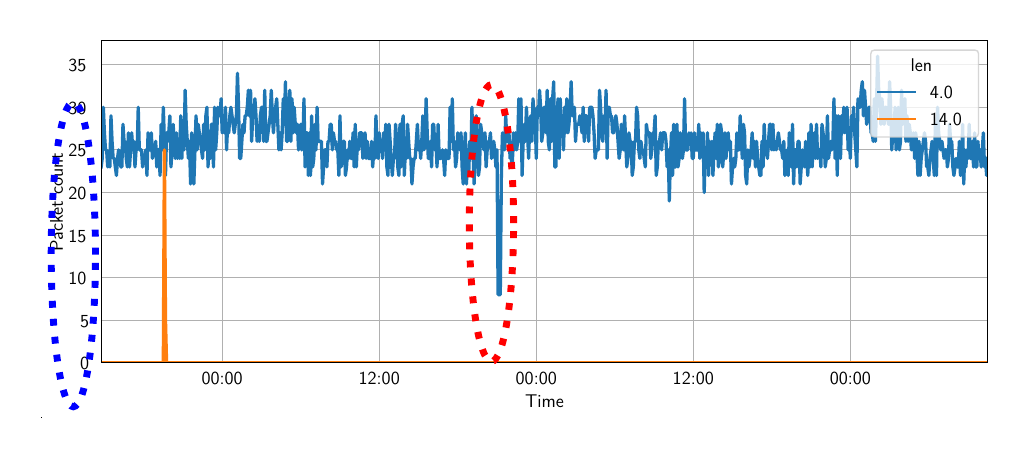
\begin{tikzpicture}
            \node(A){   
            \resizebox{1\textwidth}{!}
                {
                    %% Creator: Matplotlib, PGF backend
%%
%% To include the figure in your LaTeX document, write
%%   \input{<filename>.pgf}
%%
%% Make sure the required packages are loaded in your preamble
%%   \usepackage{pgf}
%%
%% Also ensure that all the required font packages are loaded; for instance,
%% the lmodern package is sometimes necessary when using math font.
%%   \usepackage{lmodern}
%%
%% Figures using additional raster images can only be included by \input if
%% they are in the same directory as the main LaTeX file. For loading figures
%% from other directories you can use the `import` package
%%   \usepackage{import}
%%
%% and then include the figures with
%%   \import{<path to file>}{<filename>.pgf}
%%
%% Matplotlib used the following preamble
%%   \usepackage{fontspec}
%%   \setmainfont{DejaVuSerif.ttf}[Path=\detokenize{/home/ankimme/fit/ibt/env/lib/python3.10/site-packages/matplotlib/mpl-data/fonts/ttf/}]
%%   \setsansfont{DejaVuSans.ttf}[Path=\detokenize{/home/ankimme/fit/ibt/env/lib/python3.10/site-packages/matplotlib/mpl-data/fonts/ttf/}]
%%   \setmonofont{DejaVuSansMono.ttf}[Path=\detokenize{/home/ankimme/fit/ibt/env/lib/python3.10/site-packages/matplotlib/mpl-data/fonts/ttf/}]
%%
\begingroup%
\makeatletter%
\begin{pgfpicture}%
\pgfpathrectangle{\pgfpointorigin}{\pgfqpoint{10.000000in}{4.000000in}}%
\pgfusepath{use as bounding box, clip}%
\begin{pgfscope}%
\pgfsetbuttcap%
\pgfsetmiterjoin%
\pgfsetlinewidth{0.000000pt}%
\definecolor{currentstroke}{rgb}{1.000000,1.000000,1.000000}%
\pgfsetstrokecolor{currentstroke}%
\pgfsetstrokeopacity{0.000000}%
\pgfsetdash{}{0pt}%
\pgfpathmoveto{\pgfqpoint{0.000000in}{0.000000in}}%
\pgfpathlineto{\pgfqpoint{10.000000in}{0.000000in}}%
\pgfpathlineto{\pgfqpoint{10.000000in}{4.000000in}}%
\pgfpathlineto{\pgfqpoint{0.000000in}{4.000000in}}%
\pgfpathlineto{\pgfqpoint{0.000000in}{0.000000in}}%
\pgfpathclose%
\pgfusepath{}%
\end{pgfscope}%
\begin{pgfscope}%
\pgfsetbuttcap%
\pgfsetmiterjoin%
\definecolor{currentfill}{rgb}{1.000000,1.000000,1.000000}%
\pgfsetfillcolor{currentfill}%
\pgfsetlinewidth{0.000000pt}%
\definecolor{currentstroke}{rgb}{0.000000,0.000000,0.000000}%
\pgfsetstrokecolor{currentstroke}%
\pgfsetstrokeopacity{0.000000}%
\pgfsetdash{}{0pt}%
\pgfpathmoveto{\pgfqpoint{0.630049in}{0.570804in}}%
\pgfpathlineto{\pgfqpoint{9.958330in}{0.570804in}}%
\pgfpathlineto{\pgfqpoint{9.958330in}{3.958330in}}%
\pgfpathlineto{\pgfqpoint{0.630049in}{3.958330in}}%
\pgfpathlineto{\pgfqpoint{0.630049in}{0.570804in}}%
\pgfpathclose%
\pgfusepath{fill}%
\end{pgfscope}%
\begin{pgfscope}%
\pgfpathrectangle{\pgfqpoint{0.630049in}{0.570804in}}{\pgfqpoint{9.328281in}{3.387526in}}%
\pgfusepath{clip}%
\pgfsetrectcap%
\pgfsetroundjoin%
\pgfsetlinewidth{0.803000pt}%
\definecolor{currentstroke}{rgb}{0.690196,0.690196,0.690196}%
\pgfsetstrokecolor{currentstroke}%
\pgfsetdash{}{0pt}%
\pgfpathmoveto{\pgfqpoint{1.903652in}{0.570804in}}%
\pgfpathlineto{\pgfqpoint{1.903652in}{3.958330in}}%
\pgfusepath{stroke}%
\end{pgfscope}%
\begin{pgfscope}%
\pgfsetbuttcap%
\pgfsetroundjoin%
\definecolor{currentfill}{rgb}{0.000000,0.000000,0.000000}%
\pgfsetfillcolor{currentfill}%
\pgfsetlinewidth{0.803000pt}%
\definecolor{currentstroke}{rgb}{0.000000,0.000000,0.000000}%
\pgfsetstrokecolor{currentstroke}%
\pgfsetdash{}{0pt}%
\pgfsys@defobject{currentmarker}{\pgfqpoint{0.000000in}{-0.048611in}}{\pgfqpoint{0.000000in}{0.000000in}}{%
\pgfpathmoveto{\pgfqpoint{0.000000in}{0.000000in}}%
\pgfpathlineto{\pgfqpoint{0.000000in}{-0.048611in}}%
\pgfusepath{stroke,fill}%
}%
\begin{pgfscope}%
\pgfsys@transformshift{1.903652in}{0.570804in}%
\pgfsys@useobject{currentmarker}{}%
\end{pgfscope}%
\end{pgfscope}%
\begin{pgfscope}%
\definecolor{textcolor}{rgb}{0.000000,0.000000,0.000000}%
\pgfsetstrokecolor{textcolor}%
\pgfsetfillcolor{textcolor}%
\pgftext[x=1.903652in,y=0.473582in,,top]{\color{textcolor}\sffamily\fontsize{14.000000}{16.800000}\selectfont 00:00}%
\end{pgfscope}%
\begin{pgfscope}%
\pgfpathrectangle{\pgfqpoint{0.630049in}{0.570804in}}{\pgfqpoint{9.328281in}{3.387526in}}%
\pgfusepath{clip}%
\pgfsetrectcap%
\pgfsetroundjoin%
\pgfsetlinewidth{0.803000pt}%
\definecolor{currentstroke}{rgb}{0.690196,0.690196,0.690196}%
\pgfsetstrokecolor{currentstroke}%
\pgfsetdash{}{0pt}%
\pgfpathmoveto{\pgfqpoint{3.555893in}{0.570804in}}%
\pgfpathlineto{\pgfqpoint{3.555893in}{3.958330in}}%
\pgfusepath{stroke}%
\end{pgfscope}%
\begin{pgfscope}%
\pgfsetbuttcap%
\pgfsetroundjoin%
\definecolor{currentfill}{rgb}{0.000000,0.000000,0.000000}%
\pgfsetfillcolor{currentfill}%
\pgfsetlinewidth{0.803000pt}%
\definecolor{currentstroke}{rgb}{0.000000,0.000000,0.000000}%
\pgfsetstrokecolor{currentstroke}%
\pgfsetdash{}{0pt}%
\pgfsys@defobject{currentmarker}{\pgfqpoint{0.000000in}{-0.048611in}}{\pgfqpoint{0.000000in}{0.000000in}}{%
\pgfpathmoveto{\pgfqpoint{0.000000in}{0.000000in}}%
\pgfpathlineto{\pgfqpoint{0.000000in}{-0.048611in}}%
\pgfusepath{stroke,fill}%
}%
\begin{pgfscope}%
\pgfsys@transformshift{3.555893in}{0.570804in}%
\pgfsys@useobject{currentmarker}{}%
\end{pgfscope}%
\end{pgfscope}%
\begin{pgfscope}%
\definecolor{textcolor}{rgb}{0.000000,0.000000,0.000000}%
\pgfsetstrokecolor{textcolor}%
\pgfsetfillcolor{textcolor}%
\pgftext[x=3.555893in,y=0.473582in,,top]{\color{textcolor}\sffamily\fontsize{14.000000}{16.800000}\selectfont 12:00}%
\end{pgfscope}%
\begin{pgfscope}%
\pgfpathrectangle{\pgfqpoint{0.630049in}{0.570804in}}{\pgfqpoint{9.328281in}{3.387526in}}%
\pgfusepath{clip}%
\pgfsetrectcap%
\pgfsetroundjoin%
\pgfsetlinewidth{0.803000pt}%
\definecolor{currentstroke}{rgb}{0.690196,0.690196,0.690196}%
\pgfsetstrokecolor{currentstroke}%
\pgfsetdash{}{0pt}%
\pgfpathmoveto{\pgfqpoint{5.208135in}{0.570804in}}%
\pgfpathlineto{\pgfqpoint{5.208135in}{3.958330in}}%
\pgfusepath{stroke}%
\end{pgfscope}%
\begin{pgfscope}%
\pgfsetbuttcap%
\pgfsetroundjoin%
\definecolor{currentfill}{rgb}{0.000000,0.000000,0.000000}%
\pgfsetfillcolor{currentfill}%
\pgfsetlinewidth{0.803000pt}%
\definecolor{currentstroke}{rgb}{0.000000,0.000000,0.000000}%
\pgfsetstrokecolor{currentstroke}%
\pgfsetdash{}{0pt}%
\pgfsys@defobject{currentmarker}{\pgfqpoint{0.000000in}{-0.048611in}}{\pgfqpoint{0.000000in}{0.000000in}}{%
\pgfpathmoveto{\pgfqpoint{0.000000in}{0.000000in}}%
\pgfpathlineto{\pgfqpoint{0.000000in}{-0.048611in}}%
\pgfusepath{stroke,fill}%
}%
\begin{pgfscope}%
\pgfsys@transformshift{5.208135in}{0.570804in}%
\pgfsys@useobject{currentmarker}{}%
\end{pgfscope}%
\end{pgfscope}%
\begin{pgfscope}%
\definecolor{textcolor}{rgb}{0.000000,0.000000,0.000000}%
\pgfsetstrokecolor{textcolor}%
\pgfsetfillcolor{textcolor}%
\pgftext[x=5.208135in,y=0.473582in,,top]{\color{textcolor}\sffamily\fontsize{14.000000}{16.800000}\selectfont 00:00}%
\end{pgfscope}%
\begin{pgfscope}%
\pgfpathrectangle{\pgfqpoint{0.630049in}{0.570804in}}{\pgfqpoint{9.328281in}{3.387526in}}%
\pgfusepath{clip}%
\pgfsetrectcap%
\pgfsetroundjoin%
\pgfsetlinewidth{0.803000pt}%
\definecolor{currentstroke}{rgb}{0.690196,0.690196,0.690196}%
\pgfsetstrokecolor{currentstroke}%
\pgfsetdash{}{0pt}%
\pgfpathmoveto{\pgfqpoint{6.860377in}{0.570804in}}%
\pgfpathlineto{\pgfqpoint{6.860377in}{3.958330in}}%
\pgfusepath{stroke}%
\end{pgfscope}%
\begin{pgfscope}%
\pgfsetbuttcap%
\pgfsetroundjoin%
\definecolor{currentfill}{rgb}{0.000000,0.000000,0.000000}%
\pgfsetfillcolor{currentfill}%
\pgfsetlinewidth{0.803000pt}%
\definecolor{currentstroke}{rgb}{0.000000,0.000000,0.000000}%
\pgfsetstrokecolor{currentstroke}%
\pgfsetdash{}{0pt}%
\pgfsys@defobject{currentmarker}{\pgfqpoint{0.000000in}{-0.048611in}}{\pgfqpoint{0.000000in}{0.000000in}}{%
\pgfpathmoveto{\pgfqpoint{0.000000in}{0.000000in}}%
\pgfpathlineto{\pgfqpoint{0.000000in}{-0.048611in}}%
\pgfusepath{stroke,fill}%
}%
\begin{pgfscope}%
\pgfsys@transformshift{6.860377in}{0.570804in}%
\pgfsys@useobject{currentmarker}{}%
\end{pgfscope}%
\end{pgfscope}%
\begin{pgfscope}%
\definecolor{textcolor}{rgb}{0.000000,0.000000,0.000000}%
\pgfsetstrokecolor{textcolor}%
\pgfsetfillcolor{textcolor}%
\pgftext[x=6.860377in,y=0.473582in,,top]{\color{textcolor}\sffamily\fontsize{14.000000}{16.800000}\selectfont 12:00}%
\end{pgfscope}%
\begin{pgfscope}%
\pgfpathrectangle{\pgfqpoint{0.630049in}{0.570804in}}{\pgfqpoint{9.328281in}{3.387526in}}%
\pgfusepath{clip}%
\pgfsetrectcap%
\pgfsetroundjoin%
\pgfsetlinewidth{0.803000pt}%
\definecolor{currentstroke}{rgb}{0.690196,0.690196,0.690196}%
\pgfsetstrokecolor{currentstroke}%
\pgfsetdash{}{0pt}%
\pgfpathmoveto{\pgfqpoint{8.512619in}{0.570804in}}%
\pgfpathlineto{\pgfqpoint{8.512619in}{3.958330in}}%
\pgfusepath{stroke}%
\end{pgfscope}%
\begin{pgfscope}%
\pgfsetbuttcap%
\pgfsetroundjoin%
\definecolor{currentfill}{rgb}{0.000000,0.000000,0.000000}%
\pgfsetfillcolor{currentfill}%
\pgfsetlinewidth{0.803000pt}%
\definecolor{currentstroke}{rgb}{0.000000,0.000000,0.000000}%
\pgfsetstrokecolor{currentstroke}%
\pgfsetdash{}{0pt}%
\pgfsys@defobject{currentmarker}{\pgfqpoint{0.000000in}{-0.048611in}}{\pgfqpoint{0.000000in}{0.000000in}}{%
\pgfpathmoveto{\pgfqpoint{0.000000in}{0.000000in}}%
\pgfpathlineto{\pgfqpoint{0.000000in}{-0.048611in}}%
\pgfusepath{stroke,fill}%
}%
\begin{pgfscope}%
\pgfsys@transformshift{8.512619in}{0.570804in}%
\pgfsys@useobject{currentmarker}{}%
\end{pgfscope}%
\end{pgfscope}%
\begin{pgfscope}%
\definecolor{textcolor}{rgb}{0.000000,0.000000,0.000000}%
\pgfsetstrokecolor{textcolor}%
\pgfsetfillcolor{textcolor}%
\pgftext[x=8.512619in,y=0.473582in,,top]{\color{textcolor}\sffamily\fontsize{14.000000}{16.800000}\selectfont 00:00}%
\end{pgfscope}%
\begin{pgfscope}%
\definecolor{textcolor}{rgb}{0.000000,0.000000,0.000000}%
\pgfsetstrokecolor{textcolor}%
\pgfsetfillcolor{textcolor}%
\pgftext[x=5.294189in,y=0.229848in,,top]{\color{textcolor}\sffamily\fontsize{14.000000}{16.800000}\selectfont Time}%
\end{pgfscope}%
\begin{pgfscope}%
\pgfpathrectangle{\pgfqpoint{0.630049in}{0.570804in}}{\pgfqpoint{9.328281in}{3.387526in}}%
\pgfusepath{clip}%
\pgfsetrectcap%
\pgfsetroundjoin%
\pgfsetlinewidth{0.803000pt}%
\definecolor{currentstroke}{rgb}{0.690196,0.690196,0.690196}%
\pgfsetstrokecolor{currentstroke}%
\pgfsetdash{}{0pt}%
\pgfpathmoveto{\pgfqpoint{0.630049in}{0.570804in}}%
\pgfpathlineto{\pgfqpoint{9.958330in}{0.570804in}}%
\pgfusepath{stroke}%
\end{pgfscope}%
\begin{pgfscope}%
\pgfsetbuttcap%
\pgfsetroundjoin%
\definecolor{currentfill}{rgb}{0.000000,0.000000,0.000000}%
\pgfsetfillcolor{currentfill}%
\pgfsetlinewidth{0.803000pt}%
\definecolor{currentstroke}{rgb}{0.000000,0.000000,0.000000}%
\pgfsetstrokecolor{currentstroke}%
\pgfsetdash{}{0pt}%
\pgfsys@defobject{currentmarker}{\pgfqpoint{-0.048611in}{0.000000in}}{\pgfqpoint{-0.000000in}{0.000000in}}{%
\pgfpathmoveto{\pgfqpoint{-0.000000in}{0.000000in}}%
\pgfpathlineto{\pgfqpoint{-0.048611in}{0.000000in}}%
\pgfusepath{stroke,fill}%
}%
\begin{pgfscope}%
\pgfsys@transformshift{0.630049in}{0.570804in}%
\pgfsys@useobject{currentmarker}{}%
\end{pgfscope}%
\end{pgfscope}%
\begin{pgfscope}%
\definecolor{textcolor}{rgb}{0.000000,0.000000,0.000000}%
\pgfsetstrokecolor{textcolor}%
\pgfsetfillcolor{textcolor}%
\pgftext[x=0.409115in, y=0.496938in, left, base]{\color{textcolor}\sffamily\fontsize{14.000000}{16.800000}\selectfont 0}%
\end{pgfscope}%
\begin{pgfscope}%
\pgfpathrectangle{\pgfqpoint{0.630049in}{0.570804in}}{\pgfqpoint{9.328281in}{3.387526in}}%
\pgfusepath{clip}%
\pgfsetrectcap%
\pgfsetroundjoin%
\pgfsetlinewidth{0.803000pt}%
\definecolor{currentstroke}{rgb}{0.690196,0.690196,0.690196}%
\pgfsetstrokecolor{currentstroke}%
\pgfsetdash{}{0pt}%
\pgfpathmoveto{\pgfqpoint{0.630049in}{1.018889in}}%
\pgfpathlineto{\pgfqpoint{9.958330in}{1.018889in}}%
\pgfusepath{stroke}%
\end{pgfscope}%
\begin{pgfscope}%
\pgfsetbuttcap%
\pgfsetroundjoin%
\definecolor{currentfill}{rgb}{0.000000,0.000000,0.000000}%
\pgfsetfillcolor{currentfill}%
\pgfsetlinewidth{0.803000pt}%
\definecolor{currentstroke}{rgb}{0.000000,0.000000,0.000000}%
\pgfsetstrokecolor{currentstroke}%
\pgfsetdash{}{0pt}%
\pgfsys@defobject{currentmarker}{\pgfqpoint{-0.048611in}{0.000000in}}{\pgfqpoint{-0.000000in}{0.000000in}}{%
\pgfpathmoveto{\pgfqpoint{-0.000000in}{0.000000in}}%
\pgfpathlineto{\pgfqpoint{-0.048611in}{0.000000in}}%
\pgfusepath{stroke,fill}%
}%
\begin{pgfscope}%
\pgfsys@transformshift{0.630049in}{1.018889in}%
\pgfsys@useobject{currentmarker}{}%
\end{pgfscope}%
\end{pgfscope}%
\begin{pgfscope}%
\definecolor{textcolor}{rgb}{0.000000,0.000000,0.000000}%
\pgfsetstrokecolor{textcolor}%
\pgfsetfillcolor{textcolor}%
\pgftext[x=0.409115in, y=0.945023in, left, base]{\color{textcolor}\sffamily\fontsize{14.000000}{16.800000}\selectfont 5}%
\end{pgfscope}%
\begin{pgfscope}%
\pgfpathrectangle{\pgfqpoint{0.630049in}{0.570804in}}{\pgfqpoint{9.328281in}{3.387526in}}%
\pgfusepath{clip}%
\pgfsetrectcap%
\pgfsetroundjoin%
\pgfsetlinewidth{0.803000pt}%
\definecolor{currentstroke}{rgb}{0.690196,0.690196,0.690196}%
\pgfsetstrokecolor{currentstroke}%
\pgfsetdash{}{0pt}%
\pgfpathmoveto{\pgfqpoint{0.630049in}{1.466975in}}%
\pgfpathlineto{\pgfqpoint{9.958330in}{1.466975in}}%
\pgfusepath{stroke}%
\end{pgfscope}%
\begin{pgfscope}%
\pgfsetbuttcap%
\pgfsetroundjoin%
\definecolor{currentfill}{rgb}{0.000000,0.000000,0.000000}%
\pgfsetfillcolor{currentfill}%
\pgfsetlinewidth{0.803000pt}%
\definecolor{currentstroke}{rgb}{0.000000,0.000000,0.000000}%
\pgfsetstrokecolor{currentstroke}%
\pgfsetdash{}{0pt}%
\pgfsys@defobject{currentmarker}{\pgfqpoint{-0.048611in}{0.000000in}}{\pgfqpoint{-0.000000in}{0.000000in}}{%
\pgfpathmoveto{\pgfqpoint{-0.000000in}{0.000000in}}%
\pgfpathlineto{\pgfqpoint{-0.048611in}{0.000000in}}%
\pgfusepath{stroke,fill}%
}%
\begin{pgfscope}%
\pgfsys@transformshift{0.630049in}{1.466975in}%
\pgfsys@useobject{currentmarker}{}%
\end{pgfscope}%
\end{pgfscope}%
\begin{pgfscope}%
\definecolor{textcolor}{rgb}{0.000000,0.000000,0.000000}%
\pgfsetstrokecolor{textcolor}%
\pgfsetfillcolor{textcolor}%
\pgftext[x=0.285404in, y=1.393109in, left, base]{\color{textcolor}\sffamily\fontsize{14.000000}{16.800000}\selectfont 10}%
\end{pgfscope}%
\begin{pgfscope}%
\pgfpathrectangle{\pgfqpoint{0.630049in}{0.570804in}}{\pgfqpoint{9.328281in}{3.387526in}}%
\pgfusepath{clip}%
\pgfsetrectcap%
\pgfsetroundjoin%
\pgfsetlinewidth{0.803000pt}%
\definecolor{currentstroke}{rgb}{0.690196,0.690196,0.690196}%
\pgfsetstrokecolor{currentstroke}%
\pgfsetdash{}{0pt}%
\pgfpathmoveto{\pgfqpoint{0.630049in}{1.915060in}}%
\pgfpathlineto{\pgfqpoint{9.958330in}{1.915060in}}%
\pgfusepath{stroke}%
\end{pgfscope}%
\begin{pgfscope}%
\pgfsetbuttcap%
\pgfsetroundjoin%
\definecolor{currentfill}{rgb}{0.000000,0.000000,0.000000}%
\pgfsetfillcolor{currentfill}%
\pgfsetlinewidth{0.803000pt}%
\definecolor{currentstroke}{rgb}{0.000000,0.000000,0.000000}%
\pgfsetstrokecolor{currentstroke}%
\pgfsetdash{}{0pt}%
\pgfsys@defobject{currentmarker}{\pgfqpoint{-0.048611in}{0.000000in}}{\pgfqpoint{-0.000000in}{0.000000in}}{%
\pgfpathmoveto{\pgfqpoint{-0.000000in}{0.000000in}}%
\pgfpathlineto{\pgfqpoint{-0.048611in}{0.000000in}}%
\pgfusepath{stroke,fill}%
}%
\begin{pgfscope}%
\pgfsys@transformshift{0.630049in}{1.915060in}%
\pgfsys@useobject{currentmarker}{}%
\end{pgfscope}%
\end{pgfscope}%
\begin{pgfscope}%
\definecolor{textcolor}{rgb}{0.000000,0.000000,0.000000}%
\pgfsetstrokecolor{textcolor}%
\pgfsetfillcolor{textcolor}%
\pgftext[x=0.285404in, y=1.841194in, left, base]{\color{textcolor}\sffamily\fontsize{14.000000}{16.800000}\selectfont 15}%
\end{pgfscope}%
\begin{pgfscope}%
\pgfpathrectangle{\pgfqpoint{0.630049in}{0.570804in}}{\pgfqpoint{9.328281in}{3.387526in}}%
\pgfusepath{clip}%
\pgfsetrectcap%
\pgfsetroundjoin%
\pgfsetlinewidth{0.803000pt}%
\definecolor{currentstroke}{rgb}{0.690196,0.690196,0.690196}%
\pgfsetstrokecolor{currentstroke}%
\pgfsetdash{}{0pt}%
\pgfpathmoveto{\pgfqpoint{0.630049in}{2.363146in}}%
\pgfpathlineto{\pgfqpoint{9.958330in}{2.363146in}}%
\pgfusepath{stroke}%
\end{pgfscope}%
\begin{pgfscope}%
\pgfsetbuttcap%
\pgfsetroundjoin%
\definecolor{currentfill}{rgb}{0.000000,0.000000,0.000000}%
\pgfsetfillcolor{currentfill}%
\pgfsetlinewidth{0.803000pt}%
\definecolor{currentstroke}{rgb}{0.000000,0.000000,0.000000}%
\pgfsetstrokecolor{currentstroke}%
\pgfsetdash{}{0pt}%
\pgfsys@defobject{currentmarker}{\pgfqpoint{-0.048611in}{0.000000in}}{\pgfqpoint{-0.000000in}{0.000000in}}{%
\pgfpathmoveto{\pgfqpoint{-0.000000in}{0.000000in}}%
\pgfpathlineto{\pgfqpoint{-0.048611in}{0.000000in}}%
\pgfusepath{stroke,fill}%
}%
\begin{pgfscope}%
\pgfsys@transformshift{0.630049in}{2.363146in}%
\pgfsys@useobject{currentmarker}{}%
\end{pgfscope}%
\end{pgfscope}%
\begin{pgfscope}%
\definecolor{textcolor}{rgb}{0.000000,0.000000,0.000000}%
\pgfsetstrokecolor{textcolor}%
\pgfsetfillcolor{textcolor}%
\pgftext[x=0.285404in, y=2.289280in, left, base]{\color{textcolor}\sffamily\fontsize{14.000000}{16.800000}\selectfont 20}%
\end{pgfscope}%
\begin{pgfscope}%
\pgfpathrectangle{\pgfqpoint{0.630049in}{0.570804in}}{\pgfqpoint{9.328281in}{3.387526in}}%
\pgfusepath{clip}%
\pgfsetrectcap%
\pgfsetroundjoin%
\pgfsetlinewidth{0.803000pt}%
\definecolor{currentstroke}{rgb}{0.690196,0.690196,0.690196}%
\pgfsetstrokecolor{currentstroke}%
\pgfsetdash{}{0pt}%
\pgfpathmoveto{\pgfqpoint{0.630049in}{2.811231in}}%
\pgfpathlineto{\pgfqpoint{9.958330in}{2.811231in}}%
\pgfusepath{stroke}%
\end{pgfscope}%
\begin{pgfscope}%
\pgfsetbuttcap%
\pgfsetroundjoin%
\definecolor{currentfill}{rgb}{0.000000,0.000000,0.000000}%
\pgfsetfillcolor{currentfill}%
\pgfsetlinewidth{0.803000pt}%
\definecolor{currentstroke}{rgb}{0.000000,0.000000,0.000000}%
\pgfsetstrokecolor{currentstroke}%
\pgfsetdash{}{0pt}%
\pgfsys@defobject{currentmarker}{\pgfqpoint{-0.048611in}{0.000000in}}{\pgfqpoint{-0.000000in}{0.000000in}}{%
\pgfpathmoveto{\pgfqpoint{-0.000000in}{0.000000in}}%
\pgfpathlineto{\pgfqpoint{-0.048611in}{0.000000in}}%
\pgfusepath{stroke,fill}%
}%
\begin{pgfscope}%
\pgfsys@transformshift{0.630049in}{2.811231in}%
\pgfsys@useobject{currentmarker}{}%
\end{pgfscope}%
\end{pgfscope}%
\begin{pgfscope}%
\definecolor{textcolor}{rgb}{0.000000,0.000000,0.000000}%
\pgfsetstrokecolor{textcolor}%
\pgfsetfillcolor{textcolor}%
\pgftext[x=0.285404in, y=2.737365in, left, base]{\color{textcolor}\sffamily\fontsize{14.000000}{16.800000}\selectfont 25}%
\end{pgfscope}%
\begin{pgfscope}%
\pgfpathrectangle{\pgfqpoint{0.630049in}{0.570804in}}{\pgfqpoint{9.328281in}{3.387526in}}%
\pgfusepath{clip}%
\pgfsetrectcap%
\pgfsetroundjoin%
\pgfsetlinewidth{0.803000pt}%
\definecolor{currentstroke}{rgb}{0.690196,0.690196,0.690196}%
\pgfsetstrokecolor{currentstroke}%
\pgfsetdash{}{0pt}%
\pgfpathmoveto{\pgfqpoint{0.630049in}{3.259317in}}%
\pgfpathlineto{\pgfqpoint{9.958330in}{3.259317in}}%
\pgfusepath{stroke}%
\end{pgfscope}%
\begin{pgfscope}%
\pgfsetbuttcap%
\pgfsetroundjoin%
\definecolor{currentfill}{rgb}{0.000000,0.000000,0.000000}%
\pgfsetfillcolor{currentfill}%
\pgfsetlinewidth{0.803000pt}%
\definecolor{currentstroke}{rgb}{0.000000,0.000000,0.000000}%
\pgfsetstrokecolor{currentstroke}%
\pgfsetdash{}{0pt}%
\pgfsys@defobject{currentmarker}{\pgfqpoint{-0.048611in}{0.000000in}}{\pgfqpoint{-0.000000in}{0.000000in}}{%
\pgfpathmoveto{\pgfqpoint{-0.000000in}{0.000000in}}%
\pgfpathlineto{\pgfqpoint{-0.048611in}{0.000000in}}%
\pgfusepath{stroke,fill}%
}%
\begin{pgfscope}%
\pgfsys@transformshift{0.630049in}{3.259317in}%
\pgfsys@useobject{currentmarker}{}%
\end{pgfscope}%
\end{pgfscope}%
\begin{pgfscope}%
\definecolor{textcolor}{rgb}{0.000000,0.000000,0.000000}%
\pgfsetstrokecolor{textcolor}%
\pgfsetfillcolor{textcolor}%
\pgftext[x=0.285404in, y=3.185451in, left, base]{\color{textcolor}\sffamily\fontsize{14.000000}{16.800000}\selectfont 30}%
\end{pgfscope}%
\begin{pgfscope}%
\pgfpathrectangle{\pgfqpoint{0.630049in}{0.570804in}}{\pgfqpoint{9.328281in}{3.387526in}}%
\pgfusepath{clip}%
\pgfsetrectcap%
\pgfsetroundjoin%
\pgfsetlinewidth{0.803000pt}%
\definecolor{currentstroke}{rgb}{0.690196,0.690196,0.690196}%
\pgfsetstrokecolor{currentstroke}%
\pgfsetdash{}{0pt}%
\pgfpathmoveto{\pgfqpoint{0.630049in}{3.707402in}}%
\pgfpathlineto{\pgfqpoint{9.958330in}{3.707402in}}%
\pgfusepath{stroke}%
\end{pgfscope}%
\begin{pgfscope}%
\pgfsetbuttcap%
\pgfsetroundjoin%
\definecolor{currentfill}{rgb}{0.000000,0.000000,0.000000}%
\pgfsetfillcolor{currentfill}%
\pgfsetlinewidth{0.803000pt}%
\definecolor{currentstroke}{rgb}{0.000000,0.000000,0.000000}%
\pgfsetstrokecolor{currentstroke}%
\pgfsetdash{}{0pt}%
\pgfsys@defobject{currentmarker}{\pgfqpoint{-0.048611in}{0.000000in}}{\pgfqpoint{-0.000000in}{0.000000in}}{%
\pgfpathmoveto{\pgfqpoint{-0.000000in}{0.000000in}}%
\pgfpathlineto{\pgfqpoint{-0.048611in}{0.000000in}}%
\pgfusepath{stroke,fill}%
}%
\begin{pgfscope}%
\pgfsys@transformshift{0.630049in}{3.707402in}%
\pgfsys@useobject{currentmarker}{}%
\end{pgfscope}%
\end{pgfscope}%
\begin{pgfscope}%
\definecolor{textcolor}{rgb}{0.000000,0.000000,0.000000}%
\pgfsetstrokecolor{textcolor}%
\pgfsetfillcolor{textcolor}%
\pgftext[x=0.285404in, y=3.633536in, left, base]{\color{textcolor}\sffamily\fontsize{14.000000}{16.800000}\selectfont 35}%
\end{pgfscope}%
\begin{pgfscope}%
\definecolor{textcolor}{rgb}{0.000000,0.000000,0.000000}%
\pgfsetstrokecolor{textcolor}%
\pgfsetfillcolor{textcolor}%
\pgftext[x=0.229848in,y=2.264567in,,bottom,rotate=90.000000]{\color{textcolor}\sffamily\fontsize{14.000000}{16.800000}\selectfont Packet count}%
\end{pgfscope}%
\begin{pgfscope}%
\pgfpathrectangle{\pgfqpoint{0.630049in}{0.570804in}}{\pgfqpoint{9.328281in}{3.387526in}}%
\pgfusepath{clip}%
\pgfsetrectcap%
\pgfsetroundjoin%
\pgfsetlinewidth{2.509375pt}%
\definecolor{currentstroke}{rgb}{0.121569,0.466667,0.705882}%
\pgfsetstrokecolor{currentstroke}%
\pgfsetdash{}{0pt}%
\pgfpathmoveto{\pgfqpoint{0.630049in}{2.631997in}}%
\pgfpathlineto{\pgfqpoint{0.641523in}{2.721614in}}%
\pgfpathlineto{\pgfqpoint{0.652997in}{3.259317in}}%
\pgfpathlineto{\pgfqpoint{0.664470in}{2.990465in}}%
\pgfpathlineto{\pgfqpoint{0.675944in}{2.811231in}}%
\pgfpathlineto{\pgfqpoint{0.687418in}{2.811231in}}%
\pgfpathlineto{\pgfqpoint{0.698892in}{2.631997in}}%
\pgfpathlineto{\pgfqpoint{0.710366in}{2.721614in}}%
\pgfpathlineto{\pgfqpoint{0.721840in}{2.631997in}}%
\pgfpathlineto{\pgfqpoint{0.733314in}{3.169700in}}%
\pgfpathlineto{\pgfqpoint{0.744788in}{2.900848in}}%
\pgfpathlineto{\pgfqpoint{0.756262in}{2.721614in}}%
\pgfpathlineto{\pgfqpoint{0.767736in}{2.721614in}}%
\pgfpathlineto{\pgfqpoint{0.790683in}{2.542380in}}%
\pgfpathlineto{\pgfqpoint{0.802157in}{2.721614in}}%
\pgfpathlineto{\pgfqpoint{0.813631in}{2.811231in}}%
\pgfpathlineto{\pgfqpoint{0.836579in}{2.631997in}}%
\pgfpathlineto{\pgfqpoint{0.848053in}{2.631997in}}%
\pgfpathlineto{\pgfqpoint{0.859527in}{3.080082in}}%
\pgfpathlineto{\pgfqpoint{0.871001in}{2.900848in}}%
\pgfpathlineto{\pgfqpoint{0.882475in}{2.900848in}}%
\pgfpathlineto{\pgfqpoint{0.893948in}{2.721614in}}%
\pgfpathlineto{\pgfqpoint{0.905422in}{2.631997in}}%
\pgfpathlineto{\pgfqpoint{0.916896in}{2.990465in}}%
\pgfpathlineto{\pgfqpoint{0.928370in}{2.631997in}}%
\pgfpathlineto{\pgfqpoint{0.951318in}{2.990465in}}%
\pgfpathlineto{\pgfqpoint{0.962792in}{2.811231in}}%
\pgfpathlineto{\pgfqpoint{0.974266in}{2.900848in}}%
\pgfpathlineto{\pgfqpoint{0.985740in}{2.631997in}}%
\pgfpathlineto{\pgfqpoint{0.997214in}{2.811231in}}%
\pgfpathlineto{\pgfqpoint{1.008687in}{2.811231in}}%
\pgfpathlineto{\pgfqpoint{1.020161in}{3.259317in}}%
\pgfpathlineto{\pgfqpoint{1.031635in}{2.811231in}}%
\pgfpathlineto{\pgfqpoint{1.054583in}{2.811231in}}%
\pgfpathlineto{\pgfqpoint{1.066057in}{2.631997in}}%
\pgfpathlineto{\pgfqpoint{1.077531in}{2.721614in}}%
\pgfpathlineto{\pgfqpoint{1.089005in}{2.721614in}}%
\pgfpathlineto{\pgfqpoint{1.100479in}{2.811231in}}%
\pgfpathlineto{\pgfqpoint{1.111953in}{2.542380in}}%
\pgfpathlineto{\pgfqpoint{1.123426in}{2.990465in}}%
\pgfpathlineto{\pgfqpoint{1.134900in}{2.811231in}}%
\pgfpathlineto{\pgfqpoint{1.146374in}{2.811231in}}%
\pgfpathlineto{\pgfqpoint{1.157848in}{2.990465in}}%
\pgfpathlineto{\pgfqpoint{1.169322in}{2.721614in}}%
\pgfpathlineto{\pgfqpoint{1.180796in}{2.811231in}}%
\pgfpathlineto{\pgfqpoint{1.192270in}{2.811231in}}%
\pgfpathlineto{\pgfqpoint{1.203744in}{2.900848in}}%
\pgfpathlineto{\pgfqpoint{1.215218in}{2.631997in}}%
\pgfpathlineto{\pgfqpoint{1.226692in}{2.811231in}}%
\pgfpathlineto{\pgfqpoint{1.238165in}{2.811231in}}%
\pgfpathlineto{\pgfqpoint{1.249639in}{2.542380in}}%
\pgfpathlineto{\pgfqpoint{1.261113in}{3.080082in}}%
\pgfpathlineto{\pgfqpoint{1.272587in}{2.811231in}}%
\pgfpathlineto{\pgfqpoint{1.284061in}{3.259317in}}%
\pgfpathlineto{\pgfqpoint{1.307009in}{2.542380in}}%
\pgfpathlineto{\pgfqpoint{1.318483in}{2.990465in}}%
\pgfpathlineto{\pgfqpoint{1.329957in}{2.900848in}}%
\pgfpathlineto{\pgfqpoint{1.341431in}{2.990465in}}%
\pgfpathlineto{\pgfqpoint{1.352904in}{3.169700in}}%
\pgfpathlineto{\pgfqpoint{1.364378in}{2.631997in}}%
\pgfpathlineto{\pgfqpoint{1.375852in}{2.811231in}}%
\pgfpathlineto{\pgfqpoint{1.387326in}{3.080082in}}%
\pgfpathlineto{\pgfqpoint{1.410274in}{2.721614in}}%
\pgfpathlineto{\pgfqpoint{1.421748in}{2.990465in}}%
\pgfpathlineto{\pgfqpoint{1.433222in}{2.721614in}}%
\pgfpathlineto{\pgfqpoint{1.444696in}{2.811231in}}%
\pgfpathlineto{\pgfqpoint{1.456170in}{2.721614in}}%
\pgfpathlineto{\pgfqpoint{1.467643in}{3.169700in}}%
\pgfpathlineto{\pgfqpoint{1.479117in}{2.721614in}}%
\pgfpathlineto{\pgfqpoint{1.490591in}{3.080082in}}%
\pgfpathlineto{\pgfqpoint{1.502065in}{2.811231in}}%
\pgfpathlineto{\pgfqpoint{1.513539in}{3.438551in}}%
\pgfpathlineto{\pgfqpoint{1.525013in}{3.080082in}}%
\pgfpathlineto{\pgfqpoint{1.547961in}{2.721614in}}%
\pgfpathlineto{\pgfqpoint{1.559435in}{2.900848in}}%
\pgfpathlineto{\pgfqpoint{1.570909in}{2.452763in}}%
\pgfpathlineto{\pgfqpoint{1.582383in}{2.990465in}}%
\pgfpathlineto{\pgfqpoint{1.593856in}{2.900848in}}%
\pgfpathlineto{\pgfqpoint{1.605330in}{2.452763in}}%
\pgfpathlineto{\pgfqpoint{1.628278in}{3.169700in}}%
\pgfpathlineto{\pgfqpoint{1.639752in}{2.811231in}}%
\pgfpathlineto{\pgfqpoint{1.651226in}{3.080082in}}%
\pgfpathlineto{\pgfqpoint{1.697122in}{2.721614in}}%
\pgfpathlineto{\pgfqpoint{1.708595in}{3.080082in}}%
\pgfpathlineto{\pgfqpoint{1.720069in}{2.811231in}}%
\pgfpathlineto{\pgfqpoint{1.731543in}{3.169700in}}%
\pgfpathlineto{\pgfqpoint{1.743017in}{3.259317in}}%
\pgfpathlineto{\pgfqpoint{1.754491in}{2.631997in}}%
\pgfpathlineto{\pgfqpoint{1.765965in}{2.900848in}}%
\pgfpathlineto{\pgfqpoint{1.777439in}{2.721614in}}%
\pgfpathlineto{\pgfqpoint{1.788913in}{3.080082in}}%
\pgfpathlineto{\pgfqpoint{1.800387in}{3.080082in}}%
\pgfpathlineto{\pgfqpoint{1.811861in}{2.631997in}}%
\pgfpathlineto{\pgfqpoint{1.823334in}{3.259317in}}%
\pgfpathlineto{\pgfqpoint{1.834808in}{2.811231in}}%
\pgfpathlineto{\pgfqpoint{1.846282in}{2.990465in}}%
\pgfpathlineto{\pgfqpoint{1.857756in}{3.259317in}}%
\pgfpathlineto{\pgfqpoint{1.869230in}{3.169700in}}%
\pgfpathlineto{\pgfqpoint{1.880704in}{3.169700in}}%
\pgfpathlineto{\pgfqpoint{1.892178in}{3.348934in}}%
\pgfpathlineto{\pgfqpoint{1.903652in}{2.990465in}}%
\pgfpathlineto{\pgfqpoint{1.915126in}{3.080082in}}%
\pgfpathlineto{\pgfqpoint{1.926600in}{2.990465in}}%
\pgfpathlineto{\pgfqpoint{1.938073in}{3.259317in}}%
\pgfpathlineto{\pgfqpoint{1.949547in}{2.811231in}}%
\pgfpathlineto{\pgfqpoint{1.961021in}{3.080082in}}%
\pgfpathlineto{\pgfqpoint{1.972495in}{2.990465in}}%
\pgfpathlineto{\pgfqpoint{1.983969in}{3.169700in}}%
\pgfpathlineto{\pgfqpoint{1.995443in}{3.259317in}}%
\pgfpathlineto{\pgfqpoint{2.029865in}{2.990465in}}%
\pgfpathlineto{\pgfqpoint{2.052812in}{3.169700in}}%
\pgfpathlineto{\pgfqpoint{2.064286in}{3.617785in}}%
\pgfpathlineto{\pgfqpoint{2.075760in}{3.259317in}}%
\pgfpathlineto{\pgfqpoint{2.087234in}{2.721614in}}%
\pgfpathlineto{\pgfqpoint{2.098708in}{2.721614in}}%
\pgfpathlineto{\pgfqpoint{2.121656in}{3.080082in}}%
\pgfpathlineto{\pgfqpoint{2.133130in}{2.990465in}}%
\pgfpathlineto{\pgfqpoint{2.144604in}{3.169700in}}%
\pgfpathlineto{\pgfqpoint{2.156078in}{3.169700in}}%
\pgfpathlineto{\pgfqpoint{2.167551in}{3.259317in}}%
\pgfpathlineto{\pgfqpoint{2.179025in}{3.438551in}}%
\pgfpathlineto{\pgfqpoint{2.190499in}{3.169700in}}%
\pgfpathlineto{\pgfqpoint{2.201973in}{3.438551in}}%
\pgfpathlineto{\pgfqpoint{2.213447in}{2.900848in}}%
\pgfpathlineto{\pgfqpoint{2.224921in}{3.169700in}}%
\pgfpathlineto{\pgfqpoint{2.236395in}{3.169700in}}%
\pgfpathlineto{\pgfqpoint{2.247869in}{3.348934in}}%
\pgfpathlineto{\pgfqpoint{2.259343in}{3.169700in}}%
\pgfpathlineto{\pgfqpoint{2.270817in}{2.900848in}}%
\pgfpathlineto{\pgfqpoint{2.282290in}{2.990465in}}%
\pgfpathlineto{\pgfqpoint{2.293764in}{2.900848in}}%
\pgfpathlineto{\pgfqpoint{2.305238in}{3.169700in}}%
\pgfpathlineto{\pgfqpoint{2.316712in}{3.259317in}}%
\pgfpathlineto{\pgfqpoint{2.328186in}{3.259317in}}%
\pgfpathlineto{\pgfqpoint{2.339660in}{2.900848in}}%
\pgfpathlineto{\pgfqpoint{2.351134in}{3.438551in}}%
\pgfpathlineto{\pgfqpoint{2.362608in}{2.900848in}}%
\pgfpathlineto{\pgfqpoint{2.374082in}{2.900848in}}%
\pgfpathlineto{\pgfqpoint{2.408503in}{3.169700in}}%
\pgfpathlineto{\pgfqpoint{2.419977in}{3.438551in}}%
\pgfpathlineto{\pgfqpoint{2.431451in}{3.169700in}}%
\pgfpathlineto{\pgfqpoint{2.442925in}{2.990465in}}%
\pgfpathlineto{\pgfqpoint{2.454399in}{3.169700in}}%
\pgfpathlineto{\pgfqpoint{2.477347in}{3.348934in}}%
\pgfpathlineto{\pgfqpoint{2.500295in}{2.811231in}}%
\pgfpathlineto{\pgfqpoint{2.511768in}{2.990465in}}%
\pgfpathlineto{\pgfqpoint{2.523242in}{2.811231in}}%
\pgfpathlineto{\pgfqpoint{2.534716in}{2.990465in}}%
\pgfpathlineto{\pgfqpoint{2.546190in}{3.348934in}}%
\pgfpathlineto{\pgfqpoint{2.557664in}{3.080082in}}%
\pgfpathlineto{\pgfqpoint{2.569138in}{3.528168in}}%
\pgfpathlineto{\pgfqpoint{2.580612in}{2.900848in}}%
\pgfpathlineto{\pgfqpoint{2.592086in}{2.900848in}}%
\pgfpathlineto{\pgfqpoint{2.603560in}{3.259317in}}%
\pgfpathlineto{\pgfqpoint{2.615034in}{3.438551in}}%
\pgfpathlineto{\pgfqpoint{2.626507in}{2.900848in}}%
\pgfpathlineto{\pgfqpoint{2.637981in}{3.348934in}}%
\pgfpathlineto{\pgfqpoint{2.649455in}{2.990465in}}%
\pgfpathlineto{\pgfqpoint{2.660929in}{3.259317in}}%
\pgfpathlineto{\pgfqpoint{2.672403in}{3.080082in}}%
\pgfpathlineto{\pgfqpoint{2.683877in}{2.990465in}}%
\pgfpathlineto{\pgfqpoint{2.695351in}{3.080082in}}%
\pgfpathlineto{\pgfqpoint{2.706825in}{2.811231in}}%
\pgfpathlineto{\pgfqpoint{2.718299in}{2.990465in}}%
\pgfpathlineto{\pgfqpoint{2.729773in}{3.080082in}}%
\pgfpathlineto{\pgfqpoint{2.741246in}{2.811231in}}%
\pgfpathlineto{\pgfqpoint{2.752720in}{2.900848in}}%
\pgfpathlineto{\pgfqpoint{2.764194in}{3.348934in}}%
\pgfpathlineto{\pgfqpoint{2.775668in}{2.631997in}}%
\pgfpathlineto{\pgfqpoint{2.787142in}{2.990465in}}%
\pgfpathlineto{\pgfqpoint{2.798616in}{2.990465in}}%
\pgfpathlineto{\pgfqpoint{2.810090in}{2.542380in}}%
\pgfpathlineto{\pgfqpoint{2.821564in}{2.990465in}}%
\pgfpathlineto{\pgfqpoint{2.833038in}{2.542380in}}%
\pgfpathlineto{\pgfqpoint{2.844512in}{3.169700in}}%
\pgfpathlineto{\pgfqpoint{2.855985in}{2.631997in}}%
\pgfpathlineto{\pgfqpoint{2.867459in}{2.721614in}}%
\pgfpathlineto{\pgfqpoint{2.878933in}{3.080082in}}%
\pgfpathlineto{\pgfqpoint{2.890407in}{2.811231in}}%
\pgfpathlineto{\pgfqpoint{2.901881in}{3.259317in}}%
\pgfpathlineto{\pgfqpoint{2.913355in}{2.900848in}}%
\pgfpathlineto{\pgfqpoint{2.947777in}{2.900848in}}%
\pgfpathlineto{\pgfqpoint{2.959251in}{2.452763in}}%
\pgfpathlineto{\pgfqpoint{2.982198in}{2.811231in}}%
\pgfpathlineto{\pgfqpoint{2.993672in}{2.811231in}}%
\pgfpathlineto{\pgfqpoint{3.005146in}{2.631997in}}%
\pgfpathlineto{\pgfqpoint{3.016620in}{2.900848in}}%
\pgfpathlineto{\pgfqpoint{3.028094in}{2.900848in}}%
\pgfpathlineto{\pgfqpoint{3.039568in}{3.080082in}}%
\pgfpathlineto{\pgfqpoint{3.051042in}{3.080082in}}%
\pgfpathlineto{\pgfqpoint{3.062516in}{2.811231in}}%
\pgfpathlineto{\pgfqpoint{3.073990in}{2.990465in}}%
\pgfpathlineto{\pgfqpoint{3.085463in}{2.900848in}}%
\pgfpathlineto{\pgfqpoint{3.096937in}{2.900848in}}%
\pgfpathlineto{\pgfqpoint{3.108411in}{2.811231in}}%
\pgfpathlineto{\pgfqpoint{3.119885in}{2.811231in}}%
\pgfpathlineto{\pgfqpoint{3.131359in}{2.542380in}}%
\pgfpathlineto{\pgfqpoint{3.142833in}{3.169700in}}%
\pgfpathlineto{\pgfqpoint{3.154307in}{2.631997in}}%
\pgfpathlineto{\pgfqpoint{3.165781in}{2.721614in}}%
\pgfpathlineto{\pgfqpoint{3.177255in}{2.900848in}}%
\pgfpathlineto{\pgfqpoint{3.188729in}{2.900848in}}%
\pgfpathlineto{\pgfqpoint{3.200203in}{2.542380in}}%
\pgfpathlineto{\pgfqpoint{3.211676in}{2.631997in}}%
\pgfpathlineto{\pgfqpoint{3.223150in}{2.811231in}}%
\pgfpathlineto{\pgfqpoint{3.234624in}{2.721614in}}%
\pgfpathlineto{\pgfqpoint{3.246098in}{2.900848in}}%
\pgfpathlineto{\pgfqpoint{3.257572in}{2.721614in}}%
\pgfpathlineto{\pgfqpoint{3.269046in}{2.721614in}}%
\pgfpathlineto{\pgfqpoint{3.280520in}{2.990465in}}%
\pgfpathlineto{\pgfqpoint{3.291994in}{2.631997in}}%
\pgfpathlineto{\pgfqpoint{3.303468in}{3.080082in}}%
\pgfpathlineto{\pgfqpoint{3.314942in}{2.631997in}}%
\pgfpathlineto{\pgfqpoint{3.326415in}{2.900848in}}%
\pgfpathlineto{\pgfqpoint{3.337889in}{2.811231in}}%
\pgfpathlineto{\pgfqpoint{3.349363in}{2.990465in}}%
\pgfpathlineto{\pgfqpoint{3.372311in}{2.990465in}}%
\pgfpathlineto{\pgfqpoint{3.383785in}{2.721614in}}%
\pgfpathlineto{\pgfqpoint{3.395259in}{2.811231in}}%
\pgfpathlineto{\pgfqpoint{3.406733in}{2.990465in}}%
\pgfpathlineto{\pgfqpoint{3.418207in}{2.721614in}}%
\pgfpathlineto{\pgfqpoint{3.429681in}{2.900848in}}%
\pgfpathlineto{\pgfqpoint{3.441154in}{2.721614in}}%
\pgfpathlineto{\pgfqpoint{3.464102in}{2.721614in}}%
\pgfpathlineto{\pgfqpoint{3.475576in}{2.900848in}}%
\pgfpathlineto{\pgfqpoint{3.487050in}{2.631997in}}%
\pgfpathlineto{\pgfqpoint{3.498524in}{2.811231in}}%
\pgfpathlineto{\pgfqpoint{3.509998in}{2.721614in}}%
\pgfpathlineto{\pgfqpoint{3.521472in}{3.169700in}}%
\pgfpathlineto{\pgfqpoint{3.532946in}{2.811231in}}%
\pgfpathlineto{\pgfqpoint{3.544420in}{2.721614in}}%
\pgfpathlineto{\pgfqpoint{3.555893in}{2.990465in}}%
\pgfpathlineto{\pgfqpoint{3.567367in}{2.811231in}}%
\pgfpathlineto{\pgfqpoint{3.578841in}{2.900848in}}%
\pgfpathlineto{\pgfqpoint{3.590315in}{2.721614in}}%
\pgfpathlineto{\pgfqpoint{3.601789in}{2.990465in}}%
\pgfpathlineto{\pgfqpoint{3.613263in}{2.811231in}}%
\pgfpathlineto{\pgfqpoint{3.624737in}{3.080082in}}%
\pgfpathlineto{\pgfqpoint{3.636211in}{2.631997in}}%
\pgfpathlineto{\pgfqpoint{3.647685in}{2.542380in}}%
\pgfpathlineto{\pgfqpoint{3.659159in}{3.080082in}}%
\pgfpathlineto{\pgfqpoint{3.693580in}{2.542380in}}%
\pgfpathlineto{\pgfqpoint{3.705054in}{2.721614in}}%
\pgfpathlineto{\pgfqpoint{3.716528in}{2.721614in}}%
\pgfpathlineto{\pgfqpoint{3.728002in}{3.080082in}}%
\pgfpathlineto{\pgfqpoint{3.739476in}{2.900848in}}%
\pgfpathlineto{\pgfqpoint{3.750950in}{2.631997in}}%
\pgfpathlineto{\pgfqpoint{3.762424in}{2.542380in}}%
\pgfpathlineto{\pgfqpoint{3.773898in}{3.080082in}}%
\pgfpathlineto{\pgfqpoint{3.785371in}{2.631997in}}%
\pgfpathlineto{\pgfqpoint{3.796845in}{3.080082in}}%
\pgfpathlineto{\pgfqpoint{3.808319in}{3.169700in}}%
\pgfpathlineto{\pgfqpoint{3.819793in}{2.542380in}}%
\pgfpathlineto{\pgfqpoint{3.831267in}{2.811231in}}%
\pgfpathlineto{\pgfqpoint{3.842741in}{2.721614in}}%
\pgfpathlineto{\pgfqpoint{3.854215in}{3.080082in}}%
\pgfpathlineto{\pgfqpoint{3.877163in}{2.721614in}}%
\pgfpathlineto{\pgfqpoint{3.888637in}{2.721614in}}%
\pgfpathlineto{\pgfqpoint{3.900110in}{2.452763in}}%
\pgfpathlineto{\pgfqpoint{3.911584in}{2.631997in}}%
\pgfpathlineto{\pgfqpoint{3.923058in}{2.721614in}}%
\pgfpathlineto{\pgfqpoint{3.934532in}{2.721614in}}%
\pgfpathlineto{\pgfqpoint{3.957480in}{3.080082in}}%
\pgfpathlineto{\pgfqpoint{3.968954in}{2.811231in}}%
\pgfpathlineto{\pgfqpoint{3.980428in}{2.900848in}}%
\pgfpathlineto{\pgfqpoint{3.991902in}{2.721614in}}%
\pgfpathlineto{\pgfqpoint{4.003376in}{2.900848in}}%
\pgfpathlineto{\pgfqpoint{4.014849in}{3.169700in}}%
\pgfpathlineto{\pgfqpoint{4.026323in}{2.811231in}}%
\pgfpathlineto{\pgfqpoint{4.037797in}{2.900848in}}%
\pgfpathlineto{\pgfqpoint{4.049271in}{3.348934in}}%
\pgfpathlineto{\pgfqpoint{4.060745in}{2.990465in}}%
\pgfpathlineto{\pgfqpoint{4.072219in}{2.721614in}}%
\pgfpathlineto{\pgfqpoint{4.083693in}{2.721614in}}%
\pgfpathlineto{\pgfqpoint{4.095167in}{2.900848in}}%
\pgfpathlineto{\pgfqpoint{4.106641in}{2.631997in}}%
\pgfpathlineto{\pgfqpoint{4.118115in}{3.080082in}}%
\pgfpathlineto{\pgfqpoint{4.129588in}{3.080082in}}%
\pgfpathlineto{\pgfqpoint{4.141062in}{2.811231in}}%
\pgfpathlineto{\pgfqpoint{4.152536in}{2.900848in}}%
\pgfpathlineto{\pgfqpoint{4.164010in}{2.631997in}}%
\pgfpathlineto{\pgfqpoint{4.175484in}{3.080082in}}%
\pgfpathlineto{\pgfqpoint{4.186958in}{2.721614in}}%
\pgfpathlineto{\pgfqpoint{4.209906in}{2.721614in}}%
\pgfpathlineto{\pgfqpoint{4.221380in}{2.811231in}}%
\pgfpathlineto{\pgfqpoint{4.232854in}{2.721614in}}%
\pgfpathlineto{\pgfqpoint{4.244327in}{2.542380in}}%
\pgfpathlineto{\pgfqpoint{4.255801in}{2.811231in}}%
\pgfpathlineto{\pgfqpoint{4.267275in}{2.721614in}}%
\pgfpathlineto{\pgfqpoint{4.290223in}{2.721614in}}%
\pgfpathlineto{\pgfqpoint{4.301697in}{3.259317in}}%
\pgfpathlineto{\pgfqpoint{4.313171in}{2.900848in}}%
\pgfpathlineto{\pgfqpoint{4.324645in}{3.348934in}}%
\pgfpathlineto{\pgfqpoint{4.336119in}{2.811231in}}%
\pgfpathlineto{\pgfqpoint{4.347593in}{2.900848in}}%
\pgfpathlineto{\pgfqpoint{4.359066in}{2.631997in}}%
\pgfpathlineto{\pgfqpoint{4.370540in}{2.721614in}}%
\pgfpathlineto{\pgfqpoint{4.382014in}{2.990465in}}%
\pgfpathlineto{\pgfqpoint{4.404962in}{2.811231in}}%
\pgfpathlineto{\pgfqpoint{4.416436in}{2.990465in}}%
\pgfpathlineto{\pgfqpoint{4.427910in}{2.631997in}}%
\pgfpathlineto{\pgfqpoint{4.439384in}{2.452763in}}%
\pgfpathlineto{\pgfqpoint{4.450858in}{2.811231in}}%
\pgfpathlineto{\pgfqpoint{4.462332in}{2.990465in}}%
\pgfpathlineto{\pgfqpoint{4.473805in}{2.452763in}}%
\pgfpathlineto{\pgfqpoint{4.485279in}{2.811231in}}%
\pgfpathlineto{\pgfqpoint{4.496753in}{2.542380in}}%
\pgfpathlineto{\pgfqpoint{4.508227in}{2.900848in}}%
\pgfpathlineto{\pgfqpoint{4.519701in}{2.721614in}}%
\pgfpathlineto{\pgfqpoint{4.531175in}{3.259317in}}%
\pgfpathlineto{\pgfqpoint{4.542649in}{2.811231in}}%
\pgfpathlineto{\pgfqpoint{4.554123in}{2.452763in}}%
\pgfpathlineto{\pgfqpoint{4.577071in}{3.169700in}}%
\pgfpathlineto{\pgfqpoint{4.588544in}{2.900848in}}%
\pgfpathlineto{\pgfqpoint{4.600018in}{2.542380in}}%
\pgfpathlineto{\pgfqpoint{4.611492in}{2.631997in}}%
\pgfpathlineto{\pgfqpoint{4.622966in}{3.080082in}}%
\pgfpathlineto{\pgfqpoint{4.657388in}{2.811231in}}%
\pgfpathlineto{\pgfqpoint{4.668862in}{2.990465in}}%
\pgfpathlineto{\pgfqpoint{4.680336in}{2.631997in}}%
\pgfpathlineto{\pgfqpoint{4.691810in}{2.811231in}}%
\pgfpathlineto{\pgfqpoint{4.703283in}{2.900848in}}%
\pgfpathlineto{\pgfqpoint{4.714757in}{2.900848in}}%
\pgfpathlineto{\pgfqpoint{4.726231in}{2.990465in}}%
\pgfpathlineto{\pgfqpoint{4.737705in}{2.721614in}}%
\pgfpathlineto{\pgfqpoint{4.760653in}{2.900848in}}%
\pgfpathlineto{\pgfqpoint{4.772127in}{2.811231in}}%
\pgfpathlineto{\pgfqpoint{4.783601in}{2.631997in}}%
\pgfpathlineto{\pgfqpoint{4.795075in}{2.811231in}}%
\pgfpathlineto{\pgfqpoint{4.806549in}{1.287741in}}%
\pgfpathlineto{\pgfqpoint{4.829496in}{1.287741in}}%
\pgfpathlineto{\pgfqpoint{4.840970in}{2.542380in}}%
\pgfpathlineto{\pgfqpoint{4.852444in}{2.990465in}}%
\pgfpathlineto{\pgfqpoint{4.875392in}{2.811231in}}%
\pgfpathlineto{\pgfqpoint{4.886866in}{3.169700in}}%
\pgfpathlineto{\pgfqpoint{4.898340in}{2.900848in}}%
\pgfpathlineto{\pgfqpoint{4.909814in}{2.900848in}}%
\pgfpathlineto{\pgfqpoint{4.921288in}{2.990465in}}%
\pgfpathlineto{\pgfqpoint{4.932762in}{2.721614in}}%
\pgfpathlineto{\pgfqpoint{4.944235in}{2.721614in}}%
\pgfpathlineto{\pgfqpoint{4.955709in}{2.631997in}}%
\pgfpathlineto{\pgfqpoint{4.967183in}{2.990465in}}%
\pgfpathlineto{\pgfqpoint{4.978657in}{2.811231in}}%
\pgfpathlineto{\pgfqpoint{4.990131in}{2.990465in}}%
\pgfpathlineto{\pgfqpoint{5.001605in}{2.811231in}}%
\pgfpathlineto{\pgfqpoint{5.013079in}{2.900848in}}%
\pgfpathlineto{\pgfqpoint{5.024553in}{3.348934in}}%
\pgfpathlineto{\pgfqpoint{5.036027in}{2.900848in}}%
\pgfpathlineto{\pgfqpoint{5.047501in}{3.348934in}}%
\pgfpathlineto{\pgfqpoint{5.058974in}{2.542380in}}%
\pgfpathlineto{\pgfqpoint{5.070448in}{2.900848in}}%
\pgfpathlineto{\pgfqpoint{5.081922in}{3.080082in}}%
\pgfpathlineto{\pgfqpoint{5.093396in}{2.900848in}}%
\pgfpathlineto{\pgfqpoint{5.104870in}{3.259317in}}%
\pgfpathlineto{\pgfqpoint{5.127818in}{2.721614in}}%
\pgfpathlineto{\pgfqpoint{5.139292in}{3.080082in}}%
\pgfpathlineto{\pgfqpoint{5.150766in}{3.169700in}}%
\pgfpathlineto{\pgfqpoint{5.162240in}{2.900848in}}%
\pgfpathlineto{\pgfqpoint{5.173713in}{3.348934in}}%
\pgfpathlineto{\pgfqpoint{5.185187in}{3.169700in}}%
\pgfpathlineto{\pgfqpoint{5.196661in}{3.169700in}}%
\pgfpathlineto{\pgfqpoint{5.208135in}{2.721614in}}%
\pgfpathlineto{\pgfqpoint{5.219609in}{3.259317in}}%
\pgfpathlineto{\pgfqpoint{5.231083in}{3.169700in}}%
\pgfpathlineto{\pgfqpoint{5.242557in}{3.438551in}}%
\pgfpathlineto{\pgfqpoint{5.254031in}{3.259317in}}%
\pgfpathlineto{\pgfqpoint{5.265505in}{2.900848in}}%
\pgfpathlineto{\pgfqpoint{5.276979in}{2.990465in}}%
\pgfpathlineto{\pgfqpoint{5.288452in}{3.259317in}}%
\pgfpathlineto{\pgfqpoint{5.299926in}{3.259317in}}%
\pgfpathlineto{\pgfqpoint{5.311400in}{2.990465in}}%
\pgfpathlineto{\pgfqpoint{5.322874in}{3.438551in}}%
\pgfpathlineto{\pgfqpoint{5.334348in}{2.900848in}}%
\pgfpathlineto{\pgfqpoint{5.345822in}{2.811231in}}%
\pgfpathlineto{\pgfqpoint{5.357296in}{3.348934in}}%
\pgfpathlineto{\pgfqpoint{5.368770in}{2.900848in}}%
\pgfpathlineto{\pgfqpoint{5.380244in}{3.348934in}}%
\pgfpathlineto{\pgfqpoint{5.391718in}{3.528168in}}%
\pgfpathlineto{\pgfqpoint{5.403191in}{2.631997in}}%
\pgfpathlineto{\pgfqpoint{5.414665in}{2.631997in}}%
\pgfpathlineto{\pgfqpoint{5.426139in}{3.169700in}}%
\pgfpathlineto{\pgfqpoint{5.437613in}{3.348934in}}%
\pgfpathlineto{\pgfqpoint{5.449087in}{2.721614in}}%
\pgfpathlineto{\pgfqpoint{5.460561in}{3.348934in}}%
\pgfpathlineto{\pgfqpoint{5.472035in}{2.990465in}}%
\pgfpathlineto{\pgfqpoint{5.483509in}{3.169700in}}%
\pgfpathlineto{\pgfqpoint{5.494983in}{2.811231in}}%
\pgfpathlineto{\pgfqpoint{5.506457in}{3.259317in}}%
\pgfpathlineto{\pgfqpoint{5.517930in}{2.990465in}}%
\pgfpathlineto{\pgfqpoint{5.529404in}{3.348934in}}%
\pgfpathlineto{\pgfqpoint{5.540878in}{2.990465in}}%
\pgfpathlineto{\pgfqpoint{5.552352in}{3.080082in}}%
\pgfpathlineto{\pgfqpoint{5.563826in}{3.259317in}}%
\pgfpathlineto{\pgfqpoint{5.575300in}{3.528168in}}%
\pgfpathlineto{\pgfqpoint{5.586774in}{3.169700in}}%
\pgfpathlineto{\pgfqpoint{5.598248in}{3.169700in}}%
\pgfpathlineto{\pgfqpoint{5.609722in}{3.259317in}}%
\pgfpathlineto{\pgfqpoint{5.621196in}{2.900848in}}%
\pgfpathlineto{\pgfqpoint{5.632669in}{3.080082in}}%
\pgfpathlineto{\pgfqpoint{5.655617in}{3.080082in}}%
\pgfpathlineto{\pgfqpoint{5.667091in}{3.169700in}}%
\pgfpathlineto{\pgfqpoint{5.690039in}{2.990465in}}%
\pgfpathlineto{\pgfqpoint{5.701513in}{3.259317in}}%
\pgfpathlineto{\pgfqpoint{5.712987in}{2.900848in}}%
\pgfpathlineto{\pgfqpoint{5.724461in}{3.169700in}}%
\pgfpathlineto{\pgfqpoint{5.735935in}{3.169700in}}%
\pgfpathlineto{\pgfqpoint{5.747408in}{3.080082in}}%
\pgfpathlineto{\pgfqpoint{5.758882in}{2.900848in}}%
\pgfpathlineto{\pgfqpoint{5.770356in}{3.259317in}}%
\pgfpathlineto{\pgfqpoint{5.793304in}{3.259317in}}%
\pgfpathlineto{\pgfqpoint{5.804778in}{3.169700in}}%
\pgfpathlineto{\pgfqpoint{5.816252in}{2.990465in}}%
\pgfpathlineto{\pgfqpoint{5.827726in}{2.721614in}}%
\pgfpathlineto{\pgfqpoint{5.839200in}{2.811231in}}%
\pgfpathlineto{\pgfqpoint{5.862147in}{2.811231in}}%
\pgfpathlineto{\pgfqpoint{5.873621in}{3.438551in}}%
\pgfpathlineto{\pgfqpoint{5.885095in}{3.259317in}}%
\pgfpathlineto{\pgfqpoint{5.896569in}{2.990465in}}%
\pgfpathlineto{\pgfqpoint{5.908043in}{2.900848in}}%
\pgfpathlineto{\pgfqpoint{5.919517in}{3.169700in}}%
\pgfpathlineto{\pgfqpoint{5.930991in}{2.990465in}}%
\pgfpathlineto{\pgfqpoint{5.942465in}{3.438551in}}%
\pgfpathlineto{\pgfqpoint{5.953939in}{2.721614in}}%
\pgfpathlineto{\pgfqpoint{5.965413in}{3.259317in}}%
\pgfpathlineto{\pgfqpoint{5.976886in}{3.259317in}}%
\pgfpathlineto{\pgfqpoint{5.988360in}{3.169700in}}%
\pgfpathlineto{\pgfqpoint{5.999834in}{3.169700in}}%
\pgfpathlineto{\pgfqpoint{6.011308in}{2.990465in}}%
\pgfpathlineto{\pgfqpoint{6.022782in}{2.990465in}}%
\pgfpathlineto{\pgfqpoint{6.045730in}{3.169700in}}%
\pgfpathlineto{\pgfqpoint{6.057204in}{3.080082in}}%
\pgfpathlineto{\pgfqpoint{6.080152in}{2.721614in}}%
\pgfpathlineto{\pgfqpoint{6.091625in}{2.811231in}}%
\pgfpathlineto{\pgfqpoint{6.103099in}{3.080082in}}%
\pgfpathlineto{\pgfqpoint{6.114573in}{2.900848in}}%
\pgfpathlineto{\pgfqpoint{6.126047in}{2.811231in}}%
\pgfpathlineto{\pgfqpoint{6.137521in}{3.169700in}}%
\pgfpathlineto{\pgfqpoint{6.160469in}{2.631997in}}%
\pgfpathlineto{\pgfqpoint{6.171943in}{2.721614in}}%
\pgfpathlineto{\pgfqpoint{6.183417in}{2.990465in}}%
\pgfpathlineto{\pgfqpoint{6.194891in}{2.900848in}}%
\pgfpathlineto{\pgfqpoint{6.206364in}{2.900848in}}%
\pgfpathlineto{\pgfqpoint{6.217838in}{2.542380in}}%
\pgfpathlineto{\pgfqpoint{6.229312in}{2.631997in}}%
\pgfpathlineto{\pgfqpoint{6.240786in}{2.900848in}}%
\pgfpathlineto{\pgfqpoint{6.252260in}{2.900848in}}%
\pgfpathlineto{\pgfqpoint{6.263734in}{3.259317in}}%
\pgfpathlineto{\pgfqpoint{6.275208in}{3.169700in}}%
\pgfpathlineto{\pgfqpoint{6.286682in}{2.811231in}}%
\pgfpathlineto{\pgfqpoint{6.298156in}{2.721614in}}%
\pgfpathlineto{\pgfqpoint{6.309630in}{2.900848in}}%
\pgfpathlineto{\pgfqpoint{6.321103in}{2.811231in}}%
\pgfpathlineto{\pgfqpoint{6.332577in}{2.811231in}}%
\pgfpathlineto{\pgfqpoint{6.355525in}{2.631997in}}%
\pgfpathlineto{\pgfqpoint{6.366999in}{3.080082in}}%
\pgfpathlineto{\pgfqpoint{6.378473in}{2.990465in}}%
\pgfpathlineto{\pgfqpoint{6.401421in}{2.990465in}}%
\pgfpathlineto{\pgfqpoint{6.412895in}{2.721614in}}%
\pgfpathlineto{\pgfqpoint{6.424369in}{2.811231in}}%
\pgfpathlineto{\pgfqpoint{6.435842in}{2.990465in}}%
\pgfpathlineto{\pgfqpoint{6.447316in}{2.990465in}}%
\pgfpathlineto{\pgfqpoint{6.458790in}{3.169700in}}%
\pgfpathlineto{\pgfqpoint{6.470264in}{2.542380in}}%
\pgfpathlineto{\pgfqpoint{6.481738in}{2.631997in}}%
\pgfpathlineto{\pgfqpoint{6.493212in}{2.900848in}}%
\pgfpathlineto{\pgfqpoint{6.504686in}{2.900848in}}%
\pgfpathlineto{\pgfqpoint{6.516160in}{2.990465in}}%
\pgfpathlineto{\pgfqpoint{6.527634in}{2.811231in}}%
\pgfpathlineto{\pgfqpoint{6.539108in}{2.990465in}}%
\pgfpathlineto{\pgfqpoint{6.562055in}{2.990465in}}%
\pgfpathlineto{\pgfqpoint{6.573529in}{2.900848in}}%
\pgfpathlineto{\pgfqpoint{6.585003in}{2.631997in}}%
\pgfpathlineto{\pgfqpoint{6.596477in}{2.811231in}}%
\pgfpathlineto{\pgfqpoint{6.607951in}{2.273529in}}%
\pgfpathlineto{\pgfqpoint{6.619425in}{2.721614in}}%
\pgfpathlineto{\pgfqpoint{6.630899in}{2.990465in}}%
\pgfpathlineto{\pgfqpoint{6.642373in}{2.542380in}}%
\pgfpathlineto{\pgfqpoint{6.653847in}{3.080082in}}%
\pgfpathlineto{\pgfqpoint{6.665321in}{2.631997in}}%
\pgfpathlineto{\pgfqpoint{6.676794in}{2.631997in}}%
\pgfpathlineto{\pgfqpoint{6.688268in}{3.080082in}}%
\pgfpathlineto{\pgfqpoint{6.699742in}{2.631997in}}%
\pgfpathlineto{\pgfqpoint{6.711216in}{2.721614in}}%
\pgfpathlineto{\pgfqpoint{6.722690in}{2.990465in}}%
\pgfpathlineto{\pgfqpoint{6.734164in}{2.811231in}}%
\pgfpathlineto{\pgfqpoint{6.745638in}{2.721614in}}%
\pgfpathlineto{\pgfqpoint{6.757112in}{2.811231in}}%
\pgfpathlineto{\pgfqpoint{6.768586in}{3.348934in}}%
\pgfpathlineto{\pgfqpoint{6.780060in}{2.811231in}}%
\pgfpathlineto{\pgfqpoint{6.803007in}{2.811231in}}%
\pgfpathlineto{\pgfqpoint{6.814481in}{2.990465in}}%
\pgfpathlineto{\pgfqpoint{6.825955in}{2.900848in}}%
\pgfpathlineto{\pgfqpoint{6.837429in}{2.990465in}}%
\pgfpathlineto{\pgfqpoint{6.848903in}{2.721614in}}%
\pgfpathlineto{\pgfqpoint{6.860377in}{2.721614in}}%
\pgfpathlineto{\pgfqpoint{6.871851in}{2.990465in}}%
\pgfpathlineto{\pgfqpoint{6.883325in}{2.811231in}}%
\pgfpathlineto{\pgfqpoint{6.906272in}{2.811231in}}%
\pgfpathlineto{\pgfqpoint{6.917746in}{3.080082in}}%
\pgfpathlineto{\pgfqpoint{6.929220in}{2.721614in}}%
\pgfpathlineto{\pgfqpoint{6.940694in}{2.990465in}}%
\pgfpathlineto{\pgfqpoint{6.952168in}{2.811231in}}%
\pgfpathlineto{\pgfqpoint{6.963642in}{2.990465in}}%
\pgfpathlineto{\pgfqpoint{6.975116in}{2.363146in}}%
\pgfpathlineto{\pgfqpoint{6.986590in}{2.811231in}}%
\pgfpathlineto{\pgfqpoint{6.998064in}{2.721614in}}%
\pgfpathlineto{\pgfqpoint{7.009538in}{2.990465in}}%
\pgfpathlineto{\pgfqpoint{7.021011in}{2.542380in}}%
\pgfpathlineto{\pgfqpoint{7.032485in}{2.900848in}}%
\pgfpathlineto{\pgfqpoint{7.043959in}{2.721614in}}%
\pgfpathlineto{\pgfqpoint{7.055433in}{2.900848in}}%
\pgfpathlineto{\pgfqpoint{7.066907in}{2.542380in}}%
\pgfpathlineto{\pgfqpoint{7.078381in}{2.811231in}}%
\pgfpathlineto{\pgfqpoint{7.089855in}{2.990465in}}%
\pgfpathlineto{\pgfqpoint{7.101329in}{2.721614in}}%
\pgfpathlineto{\pgfqpoint{7.112803in}{3.080082in}}%
\pgfpathlineto{\pgfqpoint{7.124277in}{2.631997in}}%
\pgfpathlineto{\pgfqpoint{7.135750in}{2.721614in}}%
\pgfpathlineto{\pgfqpoint{7.147224in}{3.080082in}}%
\pgfpathlineto{\pgfqpoint{7.158698in}{2.990465in}}%
\pgfpathlineto{\pgfqpoint{7.170172in}{2.631997in}}%
\pgfpathlineto{\pgfqpoint{7.193120in}{2.990465in}}%
\pgfpathlineto{\pgfqpoint{7.204594in}{2.721614in}}%
\pgfpathlineto{\pgfqpoint{7.216068in}{2.900848in}}%
\pgfpathlineto{\pgfqpoint{7.227542in}{2.990465in}}%
\pgfpathlineto{\pgfqpoint{7.239016in}{2.811231in}}%
\pgfpathlineto{\pgfqpoint{7.250489in}{2.900848in}}%
\pgfpathlineto{\pgfqpoint{7.261963in}{2.452763in}}%
\pgfpathlineto{\pgfqpoint{7.273437in}{2.631997in}}%
\pgfpathlineto{\pgfqpoint{7.284911in}{2.721614in}}%
\pgfpathlineto{\pgfqpoint{7.296385in}{2.631997in}}%
\pgfpathlineto{\pgfqpoint{7.307859in}{2.721614in}}%
\pgfpathlineto{\pgfqpoint{7.319333in}{2.990465in}}%
\pgfpathlineto{\pgfqpoint{7.330807in}{2.811231in}}%
\pgfpathlineto{\pgfqpoint{7.342281in}{2.811231in}}%
\pgfpathlineto{\pgfqpoint{7.353755in}{3.169700in}}%
\pgfpathlineto{\pgfqpoint{7.365228in}{2.900848in}}%
\pgfpathlineto{\pgfqpoint{7.376702in}{2.721614in}}%
\pgfpathlineto{\pgfqpoint{7.388176in}{3.080082in}}%
\pgfpathlineto{\pgfqpoint{7.399650in}{2.990465in}}%
\pgfpathlineto{\pgfqpoint{7.411124in}{2.542380in}}%
\pgfpathlineto{\pgfqpoint{7.422598in}{2.452763in}}%
\pgfpathlineto{\pgfqpoint{7.434072in}{2.811231in}}%
\pgfpathlineto{\pgfqpoint{7.445546in}{2.631997in}}%
\pgfpathlineto{\pgfqpoint{7.468494in}{2.811231in}}%
\pgfpathlineto{\pgfqpoint{7.479967in}{2.990465in}}%
\pgfpathlineto{\pgfqpoint{7.491441in}{2.721614in}}%
\pgfpathlineto{\pgfqpoint{7.502915in}{2.900848in}}%
\pgfpathlineto{\pgfqpoint{7.514389in}{2.631997in}}%
\pgfpathlineto{\pgfqpoint{7.525863in}{2.900848in}}%
\pgfpathlineto{\pgfqpoint{7.537337in}{2.721614in}}%
\pgfpathlineto{\pgfqpoint{7.560285in}{2.542380in}}%
\pgfpathlineto{\pgfqpoint{7.571759in}{2.542380in}}%
\pgfpathlineto{\pgfqpoint{7.583233in}{2.900848in}}%
\pgfpathlineto{\pgfqpoint{7.594706in}{2.631997in}}%
\pgfpathlineto{\pgfqpoint{7.606180in}{3.080082in}}%
\pgfpathlineto{\pgfqpoint{7.617654in}{2.811231in}}%
\pgfpathlineto{\pgfqpoint{7.629128in}{2.811231in}}%
\pgfpathlineto{\pgfqpoint{7.640602in}{2.721614in}}%
\pgfpathlineto{\pgfqpoint{7.663550in}{3.080082in}}%
\pgfpathlineto{\pgfqpoint{7.675024in}{3.080082in}}%
\pgfpathlineto{\pgfqpoint{7.686498in}{2.811231in}}%
\pgfpathlineto{\pgfqpoint{7.697972in}{3.080082in}}%
\pgfpathlineto{\pgfqpoint{7.709445in}{2.811231in}}%
\pgfpathlineto{\pgfqpoint{7.720919in}{2.900848in}}%
\pgfpathlineto{\pgfqpoint{7.732393in}{2.811231in}}%
\pgfpathlineto{\pgfqpoint{7.755341in}{2.990465in}}%
\pgfpathlineto{\pgfqpoint{7.778289in}{2.811231in}}%
\pgfpathlineto{\pgfqpoint{7.789763in}{2.811231in}}%
\pgfpathlineto{\pgfqpoint{7.801237in}{2.721614in}}%
\pgfpathlineto{\pgfqpoint{7.812711in}{2.900848in}}%
\pgfpathlineto{\pgfqpoint{7.824184in}{2.542380in}}%
\pgfpathlineto{\pgfqpoint{7.835658in}{2.631997in}}%
\pgfpathlineto{\pgfqpoint{7.847132in}{2.811231in}}%
\pgfpathlineto{\pgfqpoint{7.858606in}{2.542380in}}%
\pgfpathlineto{\pgfqpoint{7.870080in}{2.990465in}}%
\pgfpathlineto{\pgfqpoint{7.881554in}{2.721614in}}%
\pgfpathlineto{\pgfqpoint{7.893028in}{2.631997in}}%
\pgfpathlineto{\pgfqpoint{7.904502in}{3.080082in}}%
\pgfpathlineto{\pgfqpoint{7.915976in}{2.452763in}}%
\pgfpathlineto{\pgfqpoint{7.927450in}{2.811231in}}%
\pgfpathlineto{\pgfqpoint{7.938923in}{2.811231in}}%
\pgfpathlineto{\pgfqpoint{7.950397in}{2.631997in}}%
\pgfpathlineto{\pgfqpoint{7.961871in}{2.900848in}}%
\pgfpathlineto{\pgfqpoint{7.973345in}{2.900848in}}%
\pgfpathlineto{\pgfqpoint{7.984819in}{2.452763in}}%
\pgfpathlineto{\pgfqpoint{8.007767in}{2.811231in}}%
\pgfpathlineto{\pgfqpoint{8.030715in}{2.631997in}}%
\pgfpathlineto{\pgfqpoint{8.042189in}{2.900848in}}%
\pgfpathlineto{\pgfqpoint{8.065136in}{2.542380in}}%
\pgfpathlineto{\pgfqpoint{8.076610in}{2.990465in}}%
\pgfpathlineto{\pgfqpoint{8.088084in}{2.631997in}}%
\pgfpathlineto{\pgfqpoint{8.099558in}{3.080082in}}%
\pgfpathlineto{\pgfqpoint{8.111032in}{2.631997in}}%
\pgfpathlineto{\pgfqpoint{8.122506in}{2.900848in}}%
\pgfpathlineto{\pgfqpoint{8.133980in}{2.990465in}}%
\pgfpathlineto{\pgfqpoint{8.145454in}{2.721614in}}%
\pgfpathlineto{\pgfqpoint{8.156928in}{3.080082in}}%
\pgfpathlineto{\pgfqpoint{8.168401in}{2.721614in}}%
\pgfpathlineto{\pgfqpoint{8.179875in}{2.811231in}}%
\pgfpathlineto{\pgfqpoint{8.191349in}{2.811231in}}%
\pgfpathlineto{\pgfqpoint{8.202823in}{2.631997in}}%
\pgfpathlineto{\pgfqpoint{8.214297in}{3.080082in}}%
\pgfpathlineto{\pgfqpoint{8.237245in}{2.900848in}}%
\pgfpathlineto{\pgfqpoint{8.248719in}{2.631997in}}%
\pgfpathlineto{\pgfqpoint{8.260193in}{2.721614in}}%
\pgfpathlineto{\pgfqpoint{8.271667in}{3.169700in}}%
\pgfpathlineto{\pgfqpoint{8.283141in}{2.721614in}}%
\pgfpathlineto{\pgfqpoint{8.306088in}{2.900848in}}%
\pgfpathlineto{\pgfqpoint{8.317562in}{2.811231in}}%
\pgfpathlineto{\pgfqpoint{8.329036in}{2.900848in}}%
\pgfpathlineto{\pgfqpoint{8.340510in}{3.348934in}}%
\pgfpathlineto{\pgfqpoint{8.351984in}{2.721614in}}%
\pgfpathlineto{\pgfqpoint{8.363458in}{3.169700in}}%
\pgfpathlineto{\pgfqpoint{8.374932in}{2.542380in}}%
\pgfpathlineto{\pgfqpoint{8.386406in}{3.169700in}}%
\pgfpathlineto{\pgfqpoint{8.397880in}{3.080082in}}%
\pgfpathlineto{\pgfqpoint{8.409353in}{2.721614in}}%
\pgfpathlineto{\pgfqpoint{8.420827in}{3.169700in}}%
\pgfpathlineto{\pgfqpoint{8.432301in}{2.990465in}}%
\pgfpathlineto{\pgfqpoint{8.443775in}{3.259317in}}%
\pgfpathlineto{\pgfqpoint{8.455249in}{2.990465in}}%
\pgfpathlineto{\pgfqpoint{8.466723in}{3.080082in}}%
\pgfpathlineto{\pgfqpoint{8.478197in}{3.259317in}}%
\pgfpathlineto{\pgfqpoint{8.489671in}{2.811231in}}%
\pgfpathlineto{\pgfqpoint{8.501145in}{2.990465in}}%
\pgfpathlineto{\pgfqpoint{8.512619in}{2.721614in}}%
\pgfpathlineto{\pgfqpoint{8.524092in}{3.169700in}}%
\pgfpathlineto{\pgfqpoint{8.535566in}{3.080082in}}%
\pgfpathlineto{\pgfqpoint{8.547040in}{3.259317in}}%
\pgfpathlineto{\pgfqpoint{8.558514in}{2.990465in}}%
\pgfpathlineto{\pgfqpoint{8.581462in}{2.631997in}}%
\pgfpathlineto{\pgfqpoint{8.592936in}{3.348934in}}%
\pgfpathlineto{\pgfqpoint{8.604410in}{3.259317in}}%
\pgfpathlineto{\pgfqpoint{8.615884in}{3.259317in}}%
\pgfpathlineto{\pgfqpoint{8.627358in}{3.438551in}}%
\pgfpathlineto{\pgfqpoint{8.638831in}{3.528168in}}%
\pgfpathlineto{\pgfqpoint{8.650305in}{3.169700in}}%
\pgfpathlineto{\pgfqpoint{8.661779in}{3.438551in}}%
\pgfpathlineto{\pgfqpoint{8.684727in}{3.080082in}}%
\pgfpathlineto{\pgfqpoint{8.707675in}{3.259317in}}%
\pgfpathlineto{\pgfqpoint{8.719149in}{3.259317in}}%
\pgfpathlineto{\pgfqpoint{8.730623in}{2.990465in}}%
\pgfpathlineto{\pgfqpoint{8.742097in}{2.990465in}}%
\pgfpathlineto{\pgfqpoint{8.753570in}{2.900848in}}%
\pgfpathlineto{\pgfqpoint{8.765044in}{3.348934in}}%
\pgfpathlineto{\pgfqpoint{8.776518in}{2.900848in}}%
\pgfpathlineto{\pgfqpoint{8.787992in}{3.259317in}}%
\pgfpathlineto{\pgfqpoint{8.799466in}{3.797019in}}%
\pgfpathlineto{\pgfqpoint{8.810940in}{3.438551in}}%
\pgfpathlineto{\pgfqpoint{8.822414in}{3.348934in}}%
\pgfpathlineto{\pgfqpoint{8.833888in}{3.080082in}}%
\pgfpathlineto{\pgfqpoint{8.845362in}{3.348934in}}%
\pgfpathlineto{\pgfqpoint{8.856836in}{3.169700in}}%
\pgfpathlineto{\pgfqpoint{8.868309in}{3.080082in}}%
\pgfpathlineto{\pgfqpoint{8.879783in}{3.259317in}}%
\pgfpathlineto{\pgfqpoint{8.891257in}{3.259317in}}%
\pgfpathlineto{\pgfqpoint{8.914205in}{3.080082in}}%
\pgfpathlineto{\pgfqpoint{8.925679in}{3.528168in}}%
\pgfpathlineto{\pgfqpoint{8.937153in}{3.259317in}}%
\pgfpathlineto{\pgfqpoint{8.948627in}{2.811231in}}%
\pgfpathlineto{\pgfqpoint{8.960101in}{2.990465in}}%
\pgfpathlineto{\pgfqpoint{8.971575in}{2.900848in}}%
\pgfpathlineto{\pgfqpoint{8.983048in}{3.259317in}}%
\pgfpathlineto{\pgfqpoint{8.994522in}{2.811231in}}%
\pgfpathlineto{\pgfqpoint{9.005996in}{3.169700in}}%
\pgfpathlineto{\pgfqpoint{9.017470in}{3.259317in}}%
\pgfpathlineto{\pgfqpoint{9.028944in}{2.811231in}}%
\pgfpathlineto{\pgfqpoint{9.040418in}{2.900848in}}%
\pgfpathlineto{\pgfqpoint{9.051892in}{3.438551in}}%
\pgfpathlineto{\pgfqpoint{9.063366in}{3.080082in}}%
\pgfpathlineto{\pgfqpoint{9.074840in}{3.169700in}}%
\pgfpathlineto{\pgfqpoint{9.086314in}{3.348934in}}%
\pgfpathlineto{\pgfqpoint{9.097787in}{2.900848in}}%
\pgfpathlineto{\pgfqpoint{9.109261in}{3.169700in}}%
\pgfpathlineto{\pgfqpoint{9.120735in}{2.900848in}}%
\pgfpathlineto{\pgfqpoint{9.132209in}{3.080082in}}%
\pgfpathlineto{\pgfqpoint{9.143683in}{2.990465in}}%
\pgfpathlineto{\pgfqpoint{9.155157in}{2.811231in}}%
\pgfpathlineto{\pgfqpoint{9.178105in}{2.990465in}}%
\pgfpathlineto{\pgfqpoint{9.189579in}{2.721614in}}%
\pgfpathlineto{\pgfqpoint{9.201053in}{2.990465in}}%
\pgfpathlineto{\pgfqpoint{9.212526in}{2.811231in}}%
\pgfpathlineto{\pgfqpoint{9.224000in}{2.542380in}}%
\pgfpathlineto{\pgfqpoint{9.235474in}{2.900848in}}%
\pgfpathlineto{\pgfqpoint{9.246948in}{2.542380in}}%
\pgfpathlineto{\pgfqpoint{9.258422in}{2.721614in}}%
\pgfpathlineto{\pgfqpoint{9.292844in}{2.990465in}}%
\pgfpathlineto{\pgfqpoint{9.304318in}{2.900848in}}%
\pgfpathlineto{\pgfqpoint{9.315792in}{2.631997in}}%
\pgfpathlineto{\pgfqpoint{9.327265in}{2.631997in}}%
\pgfpathlineto{\pgfqpoint{9.338739in}{2.542380in}}%
\pgfpathlineto{\pgfqpoint{9.350213in}{2.721614in}}%
\pgfpathlineto{\pgfqpoint{9.373161in}{2.900848in}}%
\pgfpathlineto{\pgfqpoint{9.396109in}{2.542380in}}%
\pgfpathlineto{\pgfqpoint{9.407583in}{3.080082in}}%
\pgfpathlineto{\pgfqpoint{9.419057in}{2.542380in}}%
\pgfpathlineto{\pgfqpoint{9.430531in}{3.259317in}}%
\pgfpathlineto{\pgfqpoint{9.442004in}{2.990465in}}%
\pgfpathlineto{\pgfqpoint{9.464952in}{2.811231in}}%
\pgfpathlineto{\pgfqpoint{9.476426in}{2.900848in}}%
\pgfpathlineto{\pgfqpoint{9.499374in}{2.721614in}}%
\pgfpathlineto{\pgfqpoint{9.510848in}{2.811231in}}%
\pgfpathlineto{\pgfqpoint{9.522322in}{2.811231in}}%
\pgfpathlineto{\pgfqpoint{9.533796in}{2.631997in}}%
\pgfpathlineto{\pgfqpoint{9.545270in}{2.721614in}}%
\pgfpathlineto{\pgfqpoint{9.556743in}{3.080082in}}%
\pgfpathlineto{\pgfqpoint{9.568217in}{2.900848in}}%
\pgfpathlineto{\pgfqpoint{9.579691in}{2.900848in}}%
\pgfpathlineto{\pgfqpoint{9.591165in}{2.631997in}}%
\pgfpathlineto{\pgfqpoint{9.602639in}{2.542380in}}%
\pgfpathlineto{\pgfqpoint{9.625587in}{2.721614in}}%
\pgfpathlineto{\pgfqpoint{9.637061in}{2.631997in}}%
\pgfpathlineto{\pgfqpoint{9.648535in}{2.631997in}}%
\pgfpathlineto{\pgfqpoint{9.660009in}{2.900848in}}%
\pgfpathlineto{\pgfqpoint{9.671482in}{2.542380in}}%
\pgfpathlineto{\pgfqpoint{9.682956in}{2.631997in}}%
\pgfpathlineto{\pgfqpoint{9.694430in}{3.080082in}}%
\pgfpathlineto{\pgfqpoint{9.705904in}{2.452763in}}%
\pgfpathlineto{\pgfqpoint{9.717378in}{2.811231in}}%
\pgfpathlineto{\pgfqpoint{9.728852in}{2.631997in}}%
\pgfpathlineto{\pgfqpoint{9.740326in}{2.811231in}}%
\pgfpathlineto{\pgfqpoint{9.751800in}{2.721614in}}%
\pgfpathlineto{\pgfqpoint{9.763274in}{3.080082in}}%
\pgfpathlineto{\pgfqpoint{9.774748in}{2.721614in}}%
\pgfpathlineto{\pgfqpoint{9.786221in}{2.721614in}}%
\pgfpathlineto{\pgfqpoint{9.797695in}{2.900848in}}%
\pgfpathlineto{\pgfqpoint{9.809169in}{2.631997in}}%
\pgfpathlineto{\pgfqpoint{9.820643in}{2.990465in}}%
\pgfpathlineto{\pgfqpoint{9.832117in}{2.631997in}}%
\pgfpathlineto{\pgfqpoint{9.843591in}{2.631997in}}%
\pgfpathlineto{\pgfqpoint{9.855065in}{2.900848in}}%
\pgfpathlineto{\pgfqpoint{9.866539in}{2.721614in}}%
\pgfpathlineto{\pgfqpoint{9.878013in}{2.811231in}}%
\pgfpathlineto{\pgfqpoint{9.889487in}{2.631997in}}%
\pgfpathlineto{\pgfqpoint{9.912434in}{2.990465in}}%
\pgfpathlineto{\pgfqpoint{9.923908in}{2.631997in}}%
\pgfpathlineto{\pgfqpoint{9.935382in}{2.721614in}}%
\pgfpathlineto{\pgfqpoint{9.946856in}{2.542380in}}%
\pgfpathlineto{\pgfqpoint{9.958330in}{2.721614in}}%
\pgfpathlineto{\pgfqpoint{9.958330in}{2.721614in}}%
\pgfusepath{stroke}%
\end{pgfscope}%
\begin{pgfscope}%
\pgfpathrectangle{\pgfqpoint{0.630049in}{0.570804in}}{\pgfqpoint{9.328281in}{3.387526in}}%
\pgfusepath{clip}%
\pgfsetrectcap%
\pgfsetroundjoin%
\pgfsetlinewidth{2.509375pt}%
\definecolor{currentstroke}{rgb}{1.000000,0.498039,0.054902}%
\pgfsetstrokecolor{currentstroke}%
\pgfsetdash{}{0pt}%
\pgfpathmoveto{\pgfqpoint{0.630049in}{0.570804in}}%
\pgfpathlineto{\pgfqpoint{1.284061in}{0.570804in}}%
\pgfpathlineto{\pgfqpoint{1.295535in}{2.811231in}}%
\pgfpathlineto{\pgfqpoint{1.307009in}{1.018889in}}%
\pgfpathlineto{\pgfqpoint{1.318483in}{0.570804in}}%
\pgfpathlineto{\pgfqpoint{9.958330in}{0.570804in}}%
\pgfpathlineto{\pgfqpoint{9.958330in}{0.570804in}}%
\pgfusepath{stroke}%
\end{pgfscope}%
\begin{pgfscope}%
\pgfsetrectcap%
\pgfsetmiterjoin%
\pgfsetlinewidth{0.803000pt}%
\definecolor{currentstroke}{rgb}{0.000000,0.000000,0.000000}%
\pgfsetstrokecolor{currentstroke}%
\pgfsetdash{}{0pt}%
\pgfpathmoveto{\pgfqpoint{0.630049in}{0.570804in}}%
\pgfpathlineto{\pgfqpoint{0.630049in}{3.958330in}}%
\pgfusepath{stroke}%
\end{pgfscope}%
\begin{pgfscope}%
\pgfsetrectcap%
\pgfsetmiterjoin%
\pgfsetlinewidth{0.803000pt}%
\definecolor{currentstroke}{rgb}{0.000000,0.000000,0.000000}%
\pgfsetstrokecolor{currentstroke}%
\pgfsetdash{}{0pt}%
\pgfpathmoveto{\pgfqpoint{9.958330in}{0.570804in}}%
\pgfpathlineto{\pgfqpoint{9.958330in}{3.958330in}}%
\pgfusepath{stroke}%
\end{pgfscope}%
\begin{pgfscope}%
\pgfsetrectcap%
\pgfsetmiterjoin%
\pgfsetlinewidth{0.803000pt}%
\definecolor{currentstroke}{rgb}{0.000000,0.000000,0.000000}%
\pgfsetstrokecolor{currentstroke}%
\pgfsetdash{}{0pt}%
\pgfpathmoveto{\pgfqpoint{0.630049in}{0.570804in}}%
\pgfpathlineto{\pgfqpoint{9.958330in}{0.570804in}}%
\pgfusepath{stroke}%
\end{pgfscope}%
\begin{pgfscope}%
\pgfsetrectcap%
\pgfsetmiterjoin%
\pgfsetlinewidth{0.803000pt}%
\definecolor{currentstroke}{rgb}{0.000000,0.000000,0.000000}%
\pgfsetstrokecolor{currentstroke}%
\pgfsetdash{}{0pt}%
\pgfpathmoveto{\pgfqpoint{0.630049in}{3.958330in}}%
\pgfpathlineto{\pgfqpoint{9.958330in}{3.958330in}}%
\pgfusepath{stroke}%
\end{pgfscope}%
\begin{pgfscope}%
\pgfsetbuttcap%
\pgfsetmiterjoin%
\definecolor{currentfill}{rgb}{1.000000,1.000000,1.000000}%
\pgfsetfillcolor{currentfill}%
\pgfsetfillopacity{0.800000}%
\pgfsetlinewidth{1.003750pt}%
\definecolor{currentstroke}{rgb}{0.800000,0.800000,0.800000}%
\pgfsetstrokecolor{currentstroke}%
\pgfsetstrokeopacity{0.800000}%
\pgfsetdash{}{0pt}%
\pgfpathmoveto{\pgfqpoint{8.767054in}{2.946574in}}%
\pgfpathlineto{\pgfqpoint{9.822219in}{2.946574in}}%
\pgfpathquadraticcurveto{\pgfqpoint{9.861108in}{2.946574in}}{\pgfqpoint{9.861108in}{2.985463in}}%
\pgfpathlineto{\pgfqpoint{9.861108in}{3.822219in}}%
\pgfpathquadraticcurveto{\pgfqpoint{9.861108in}{3.861108in}}{\pgfqpoint{9.822219in}{3.861108in}}%
\pgfpathlineto{\pgfqpoint{8.767054in}{3.861108in}}%
\pgfpathquadraticcurveto{\pgfqpoint{8.728165in}{3.861108in}}{\pgfqpoint{8.728165in}{3.822219in}}%
\pgfpathlineto{\pgfqpoint{8.728165in}{2.985463in}}%
\pgfpathquadraticcurveto{\pgfqpoint{8.728165in}{2.946574in}}{\pgfqpoint{8.767054in}{2.946574in}}%
\pgfpathlineto{\pgfqpoint{8.767054in}{2.946574in}}%
\pgfpathclose%
\pgfusepath{stroke,fill}%
\end{pgfscope}%
\begin{pgfscope}%
\definecolor{textcolor}{rgb}{0.000000,0.000000,0.000000}%
\pgfsetstrokecolor{textcolor}%
\pgfsetfillcolor{textcolor}%
\pgftext[x=9.146192in,y=3.635598in,left,base]{\color{textcolor}\sffamily\fontsize{14.000000}{16.800000}\selectfont len}%
\end{pgfscope}%
\begin{pgfscope}%
\pgfsetrectcap%
\pgfsetroundjoin%
\pgfsetlinewidth{1.505625pt}%
\definecolor{currentstroke}{rgb}{0.121569,0.466667,0.705882}%
\pgfsetstrokecolor{currentstroke}%
\pgfsetdash{}{0pt}%
\pgfpathmoveto{\pgfqpoint{8.805943in}{3.418253in}}%
\pgfpathlineto{\pgfqpoint{9.000387in}{3.418253in}}%
\pgfpathlineto{\pgfqpoint{9.194832in}{3.418253in}}%
\pgfusepath{stroke}%
\end{pgfscope}%
\begin{pgfscope}%
\definecolor{textcolor}{rgb}{0.000000,0.000000,0.000000}%
\pgfsetstrokecolor{textcolor}%
\pgfsetfillcolor{textcolor}%
\pgftext[x=9.350387in,y=3.350198in,left,base]{\color{textcolor}\sffamily\fontsize{14.000000}{16.800000}\selectfont 4.0}%
\end{pgfscope}%
\begin{pgfscope}%
\pgfsetrectcap%
\pgfsetroundjoin%
\pgfsetlinewidth{1.505625pt}%
\definecolor{currentstroke}{rgb}{1.000000,0.498039,0.054902}%
\pgfsetstrokecolor{currentstroke}%
\pgfsetdash{}{0pt}%
\pgfpathmoveto{\pgfqpoint{8.805943in}{3.132853in}}%
\pgfpathlineto{\pgfqpoint{9.000387in}{3.132853in}}%
\pgfpathlineto{\pgfqpoint{9.194832in}{3.132853in}}%
\pgfusepath{stroke}%
\end{pgfscope}%
\begin{pgfscope}%
\definecolor{textcolor}{rgb}{0.000000,0.000000,0.000000}%
\pgfsetstrokecolor{textcolor}%
\pgfsetfillcolor{textcolor}%
\pgftext[x=9.350387in,y=3.064797in,left,base]{\color{textcolor}\sffamily\fontsize{14.000000}{16.800000}\selectfont 14.0}%
\end{pgfscope}%
\end{pgfpicture}%
\makeatother%
\endgroup%

                }
            };
            \draw[blue, line width=2.5pt, loosely dotted] ([shift=({-5.6,-0.35})]A) ellipse (8pt and 55pt);
            \draw[red, line width=2.5pt, loosely dotted] ([shift=({-0.29,0.05})]A) ellipse (8pt and 50pt);
        \end{tikzpicture}   
        \captionsetup{width=0.9\linewidth}
        \caption{Graf vývoje toku vybraných hodnot atributu \emph{len}. V prvním útoku dochází k prudkému nárůstu paketů s hodnotou 14. U druhého útoku naopak dochází k poklesu paketů s hodnotou 4.}
        \label{fig:injection_len}
    \end{subfigure}
    
    \caption{Grafy ukazující vliv útoků na tok hodnot atributu \emph{asduType} a \emph{len}. Pro zvýšení přehlednosti grafů jsou zobrazeny pouze hodnoty atributů relevantní pro detekci útoků.}%
    \label{fig:injection_both}%
\end{figure}


\chapter{Závěr}

Cílem práce bylo navrhnout a naimplementovat aplikaci pro statistickou analýzu průmyslové komunikace využívající protokolu IEC 104. Před započetím vývoje aplikace bylo potřeba nastudovat celkově tři velké tématické okruhy. Prvním z nich byla tématika ICS komunikace a protokolu IEC 104, která byla důležitá pro porozumění obsahu datových sad. Dalším okruhem byly metody pro statistický popis, analýzu a zpracování dat. A to jak z teoretického hlediska (charakteristiky míry a variability), tak i z praktického (knihovny \emph{Pandas}, \emph{Seaborn}, \dots). Poslendím okruhem byla problematika návrhu a vývoje grafického uživatelského rozhraní pomocí framworku \emph{PyQt6} pro jazyk \emph{Python}.

Navržená aplikace \emph{ICS Analyzer} umožňuje uživateli načíst datovou sadu se záznamem průmyslové komunikace ve formátu \texttt{csv}. Uživatel může před provedením analýzy datovou sadu vyfiltrovat na základě pěti kritérií. Aplikace poskytuje mimo obecných statistik datové sady také vhledy, díky kterým může uživatel nalézt stabilní prvky v komunikaci. Zejména potom stabilita v počtu zachycených paketů určitého typu v čase se jeví jako dobrý ukazatel pro detekci různých druhů anomálií.

Prostoru pro budoucí rozšíření aplikace je poměrně hodně. V první řadě by bylo dobré do aplikace přidat novou kartu, která by umožňovala zkoumat korelaci mezi různými atributy datové sady. Dále by aplikace mohla nabízet nové filtrovací kritérium, které by bylo založené na hodnotě \emph{inter-arrival time}. Mezi menší možné úpravy patří přidání možnosti volby počátečního data načítané datové sady a dopočet relativního času z časového razítka.

Na závěr bych chtěl dodat, že si z práce odnáším mnoho cenných znalostí, a to zejména na poli zpracování a analýzy dat, kterému bych se chtěl v buoucím profesním životě blíže věnovat. 




%===============================================================================
